% Options for packages loaded elsewhere
%DIF LATEXDIFF DIFFERENCE FILE
%DIF DEL C:/Users/timothy.j.miller/Documents/work/SSRTWG/SSRTWG/Ecov_study/mortality/manuscript/manuscript_R1.tex   Tue Mar 31 14:07:55 2026
%DIF ADD C:/Users/timothy.j.miller/Documents/work/SSRTWG/SSRTWG/Ecov_study/mortality/manuscript/manuscript_R2.tex   Thu May  7 09:49:01 2026
\PassOptionsToPackage{unicode}{hyperref}
\PassOptionsToPackage{hyphens}{url}
\documentclass[
  12pt,
]{article}
\usepackage{xcolor}
\usepackage[margin=1in]{geometry}
\usepackage{amsmath,amssymb}
\setcounter{secnumdepth}{5}
\usepackage{iftex}
\ifPDFTeX
  \usepackage[T1]{fontenc}
  \usepackage[utf8]{inputenc}
  \usepackage{textcomp} % provide euro and other symbols
\else % if luatex or xetex
  \usepackage{unicode-math} % this also loads fontspec
  \defaultfontfeatures{Scale=MatchLowercase}
  \defaultfontfeatures[\rmfamily]{Ligatures=TeX,Scale=1}
\fi
\usepackage{lmodern}
\ifPDFTeX\else
  % xetex/luatex font selection
\fi
% Use upquote if available, for straight quotes in verbatim environments
\IfFileExists{upquote.sty}{\usepackage{upquote}}{}
\IfFileExists{microtype.sty}{% use microtype if available
  \usepackage[]{microtype}
  \UseMicrotypeSet[protrusion]{basicmath} % disable protrusion for tt fonts
}{}
\makeatletter
\@ifundefined{KOMAClassName}{% if non-KOMA class
  \IfFileExists{parskip.sty}{%
    \usepackage{parskip}
  }{% else
    \setlength{\parindent}{0pt}
    \setlength{\parskip}{6pt plus 2pt minus 1pt}}
}{% if KOMA class
  \KOMAoptions{parskip=half}}
\makeatother
\usepackage{longtable,booktabs,array}
\usepackage{calc} % for calculating minipage widths
% Correct order of tables after \paragraph or \subparagraph
\usepackage{etoolbox}
\makeatletter
\patchcmd\longtable{\par}{\if@noskipsec\mbox{}\fi\par}{}{}
\makeatother
% Allow footnotes in longtable head/foot
\IfFileExists{footnotehyper.sty}{\usepackage{footnotehyper}}{\usepackage{footnote}}
\makesavenoteenv{longtable}
\usepackage{graphicx}
\makeatletter
\newsavebox\pandoc@box
\newcommand*\pandocbounded[1]{% scales image to fit in text height/width
  \sbox\pandoc@box{#1}%
  \Gscale@div\@tempa{\textheight}{\dimexpr\ht\pandoc@box+\dp\pandoc@box\relax}%
  \Gscale@div\@tempb{\linewidth}{\wd\pandoc@box}%
  \ifdim\@tempb\p@<\@tempa\p@\let\@tempa\@tempb\fi% select the smaller of both
  \ifdim\@tempa\p@<\p@\scalebox{\@tempa}{\usebox\pandoc@box}%
  \else\usebox{\pandoc@box}%
  \fi%
}
% Set default figure placement to htbp
\def\fps@figure{htbp}
\makeatother
\setlength{\emergencystretch}{3em} % prevent overfull lines
\providecommand{\tightlist}{%
  \setlength{\itemsep}{0pt}\setlength{\parskip}{0pt}}
\usepackage[round]{natbib}
\bibliographystyle{cjfas.bst}
\usepackage{url}
\usepackage{setspace}
%\singlespacing
%\onehalfspacing
\doublespacing
\usepackage{lineno}
\linenumbers
\usepackage[belowskip=0pt,aboveskip=0pt]{caption}
\usepackage{relsize}
\usepackage{float}
\usepackage{lscape}
\usepackage{longtable}
\usepackage{amsmath,rotating}
\usepackage[scanall]{psfrag}
\usepackage{bm}
\usepackage{caption,graphics}
\usepackage{graphicx}
\usepackage{sectsty}
\usepackage{color}
\usepackage{fancyhdr}
\usepackage{xspace}
\usepackage{textcomp}
\usepackage{upgreek}
% \usepackage{booktabs}
% \usepackage{threeparttable}
\renewcommand\figurename{Fig.}
\captionsetup{labelsep=period, singlelinecheck=false}
\newcommand{\changesize}[1]{\fontsize{#1pt}{#1pt}\selectfont}
\renewcommand{\arraystretch}{1.5}
%\renewcommand\theadfont{}

\newcommand{\Fmsy}{\ensuremath{F_{\text{MSY}}}\xspace}
\newcommand{\Fspr}[1]{\ensuremath{F_{\text{{#1}\%}}}\xspace}
\usepackage{booktabs}
\usepackage{longtable}
\usepackage{array}
\usepackage{multirow}
\usepackage{wrapfig}
\usepackage{float}
\usepackage{colortbl}
\usepackage{pdflscape}
\usepackage{tabu}
\usepackage{threeparttable}
\usepackage{threeparttablex}
\usepackage[normalem]{ulem}
\usepackage{makecell}
\usepackage{xcolor}
\usepackage{bookmark}
\IfFileExists{xurl.sty}{\usepackage{xurl}}{} % add URL line breaks if available
\urlstyle{same}
\hypersetup{
  pdftitle={Factors affecting inferences on natural mortality and associated environmental effects in state-space age-structured assessment models},
%DIF 123d123
%DIF <   pdfauthor={Timothy J. Miller1,2; Gregory L. Britten3; Elizabeth N. Brooks2; Gavin Fay4; Alexander C. Hansell2; Christopher M. Legault2; Brandon Muffley5; John Wiedenmann6},
%DIF -------
  hidelinks,
  pdfcreator={LaTeX via pandoc}}

\title{Factors affecting inferences on natural mortality and associated environmental effects in state-space age-structured assessment models}
\author{\DIFdelbegin \DIFdel{Timothy J. Miller\textsuperscript{1,2} }%DIFDELCMD < \and %%%
\DIFdel{Gregory L. Britten\textsuperscript{3} }%DIFDELCMD < \and %%%
\DIFdel{Elizabeth N. Brooks\textsuperscript{2} }%DIFDELCMD < \and %%%
\DIFdel{Gavin Fay\textsuperscript{4} }%DIFDELCMD < \and %%%
\DIFdel{Alexander C. Hansell\textsuperscript{2} }%DIFDELCMD < \and %%%
\DIFdel{Christopher M. Legault\textsuperscript{2} }%DIFDELCMD < \and %%%
\DIFdel{Brandon Muffley\textsuperscript{5} }%DIFDELCMD < \and %%%
\DIFdel{John Wiedenmann\textsuperscript{6}}\DIFdelend }
\date{\DIFdelbegin \DIFdel{31 March}\DIFdelend \DIFaddbegin \vspace{-2.5em}\DIFadd{07 May}\DIFaddend , 2026}
%DIF PREAMBLE EXTENSION ADDED BY LATEXDIFF
%DIF UNDERLINE PREAMBLE %DIF PREAMBLE
\RequirePackage[normalem]{ulem} %DIF PREAMBLE
\RequirePackage{color}\definecolor{RED}{rgb}{1,0,0}\definecolor{BLUE}{rgb}{0,0,1} %DIF PREAMBLE
\providecommand{\DIFadd}[1]{{\protect\color{blue}\uwave{#1}}} %DIF PREAMBLE
\providecommand{\DIFdel}[1]{{\protect\color{red}\sout{#1}}} %DIF PREAMBLE
%DIF SAFE PREAMBLE %DIF PREAMBLE
\providecommand{\DIFaddbegin}{} %DIF PREAMBLE
\providecommand{\DIFaddend}{} %DIF PREAMBLE
\providecommand{\DIFdelbegin}{} %DIF PREAMBLE
\providecommand{\DIFdelend}{} %DIF PREAMBLE
\providecommand{\DIFmodbegin}{} %DIF PREAMBLE
\providecommand{\DIFmodend}{} %DIF PREAMBLE
%DIF FLOATSAFE PREAMBLE %DIF PREAMBLE
\providecommand{\DIFaddFL}[1]{\DIFadd{#1}} %DIF PREAMBLE
\providecommand{\DIFdelFL}[1]{\DIFdel{#1}} %DIF PREAMBLE
\providecommand{\DIFaddbeginFL}{} %DIF PREAMBLE
\providecommand{\DIFaddendFL}{} %DIF PREAMBLE
\providecommand{\DIFdelbeginFL}{} %DIF PREAMBLE
\providecommand{\DIFdelendFL}{} %DIF PREAMBLE
\providecommand{\DIFscaledelfig}{0.5}
%DIF HIGHLIGHTGRAPHICS PREAMBLE %DIF PREAMBLE
\RequirePackage{settobox} %DIF PREAMBLE
\RequirePackage{letltxmacro} %DIF PREAMBLE
\newsavebox{\DIFdelgraphicsbox} %DIF PREAMBLE
\newlength{\DIFdelgraphicswidth} %DIF PREAMBLE
\newlength{\DIFdelgraphicsheight} %DIF PREAMBLE
% store original definition of \includegraphics %DIF PREAMBLE
\LetLtxMacro{\DIFOincludegraphics}{\includegraphics} %DIF PREAMBLE
\providecommand{\DIFaddincludegraphics}[2][]{{\color{blue}\fbox{\DIFOincludegraphics[#1]{#2}}}} %DIF PREAMBLE
\providecommand{\DIFdelincludegraphics}[2][]{% %DIF PREAMBLE
\sbox{\DIFdelgraphicsbox}{\DIFOincludegraphics[#1]{#2}}% %DIF PREAMBLE
\settoboxwidth{\DIFdelgraphicswidth}{\DIFdelgraphicsbox} %DIF PREAMBLE
\settoboxtotalheight{\DIFdelgraphicsheight}{\DIFdelgraphicsbox} %DIF PREAMBLE
\scalebox{\DIFscaledelfig}{% %DIF PREAMBLE
\parbox[b]{\DIFdelgraphicswidth}{\usebox{\DIFdelgraphicsbox}\\[-\baselineskip] \rule{\DIFdelgraphicswidth}{0em}}\llap{\resizebox{\DIFdelgraphicswidth}{\DIFdelgraphicsheight}{% %DIF PREAMBLE
\setlength{\unitlength}{\DIFdelgraphicswidth}% %DIF PREAMBLE
\begin{picture}(1,1)% %DIF PREAMBLE
\thicklines\linethickness{2pt} %DIF PREAMBLE
{\color[rgb]{1,0,0}\put(0,0){\framebox(1,1){}}}% %DIF PREAMBLE
{\color[rgb]{1,0,0}\put(0,0){\line( 1,1){1}}}% %DIF PREAMBLE
{\color[rgb]{1,0,0}\put(0,1){\line(1,-1){1}}}% %DIF PREAMBLE
\end{picture}% %DIF PREAMBLE
}\hspace*{3pt}}} %DIF PREAMBLE
} %DIF PREAMBLE
\LetLtxMacro{\DIFOaddbegin}{\DIFaddbegin} %DIF PREAMBLE
\LetLtxMacro{\DIFOaddend}{\DIFaddend} %DIF PREAMBLE
\LetLtxMacro{\DIFOdelbegin}{\DIFdelbegin} %DIF PREAMBLE
\LetLtxMacro{\DIFOdelend}{\DIFdelend} %DIF PREAMBLE
\DeclareRobustCommand{\DIFaddbegin}{\DIFOaddbegin \let\includegraphics\DIFaddincludegraphics} %DIF PREAMBLE
\DeclareRobustCommand{\DIFaddend}{\DIFOaddend \let\includegraphics\DIFOincludegraphics} %DIF PREAMBLE
\DeclareRobustCommand{\DIFdelbegin}{\DIFOdelbegin \let\includegraphics\DIFdelincludegraphics} %DIF PREAMBLE
\DeclareRobustCommand{\DIFdelend}{\DIFOaddend \let\includegraphics\DIFOincludegraphics} %DIF PREAMBLE
\LetLtxMacro{\DIFOaddbeginFL}{\DIFaddbeginFL} %DIF PREAMBLE
\LetLtxMacro{\DIFOaddendFL}{\DIFaddendFL} %DIF PREAMBLE
\LetLtxMacro{\DIFOdelbeginFL}{\DIFdelbeginFL} %DIF PREAMBLE
\LetLtxMacro{\DIFOdelendFL}{\DIFdelendFL} %DIF PREAMBLE
\DeclareRobustCommand{\DIFaddbeginFL}{\DIFOaddbeginFL \let\includegraphics\DIFaddincludegraphics} %DIF PREAMBLE
\DeclareRobustCommand{\DIFaddendFL}{\DIFOaddendFL \let\includegraphics\DIFOincludegraphics} %DIF PREAMBLE
\DeclareRobustCommand{\DIFdelbeginFL}{\DIFOdelbeginFL \let\includegraphics\DIFdelincludegraphics} %DIF PREAMBLE
\DeclareRobustCommand{\DIFdelendFL}{\DIFOaddendFL \let\includegraphics\DIFOincludegraphics} %DIF PREAMBLE
%DIF AMSMATHULEM PREAMBLE %DIF PREAMBLE
\makeatletter %DIF PREAMBLE
\let\sout@orig\sout %DIF PREAMBLE
\renewcommand{\sout}[1]{\ifmmode\text{\sout@orig{\ensuremath{#1}}}\else\sout@orig{#1}\fi} %DIF PREAMBLE
\makeatother %DIF PREAMBLE
%DIF END PREAMBLE EXTENSION ADDED BY LATEXDIFF

\begin{document}
\maketitle

\DIFdelbegin \DIFdel{\(^1\)}\DIFdelend \DIFaddbegin \DIFadd{Timothy J. Miller: ORCID ID 0000-0003-1411-1206; }\DIFaddend corresponding author: \href{mailto:timothy.j.miller@noaa.gov}{\nolinkurl{timothy.j.miller@noaa.gov}}\DIFdelbegin %DIFDELCMD < \\
%DIFDELCMD < %%%
\DIFdel{\(^2\)}\DIFdelend \DIFaddbegin \DIFadd{; }\DIFaddend Northeast Fisheries Science Center, Woods Hole Laboratory, 166 Water Street, Woods Hole, MA 02543 USA\\
\DIFdelbegin \DIFdel{\(^3\)}\DIFdelend \DIFaddbegin \strut \\
\DIFadd{Gregory L. Britten: ORCID ID 0000-0003-1391-9086; }\DIFaddend Biology Department, Woods Hole Oceanographic Institution, 266 Woods Hole Rd. Woods Hole, MA, USA\\
\DIFdelbegin \DIFdel{\(^4\)}\DIFdelend \DIFaddbegin \strut \\
\DIFadd{Elizabeth N. Brooks: ORCID ID 0000-0002-9142-4372; Northeast Fisheries Science Center, Woods Hole Laboratory, 166 Water Street, Woods Hole, MA 02543 USA}\\
\strut \\
\DIFadd{Gavin Fay: ORCID ID 0000-0003-0425-9952; }\DIFaddend Department of Fisheries Oceanography, School for Marine Science and Technology, University of Massachusetts Dartmouth, 836 S Rodney French Boulevard, New Bedford, MA \DIFdelbegin \DIFdel{02744}\DIFdelend \DIFaddbegin \DIFadd{02740}\DIFaddend , USA\\
\DIFdelbegin \DIFdel{\(^5\)}\DIFdelend \DIFaddbegin \strut \\
\DIFadd{Alexander C. Hansell: ORCID ID 0000-0001-7827-1749; Northeast Fisheries Science Center, Woods Hole Laboratory, 166 Water Street, Woods Hole, MA 02543 USA}\\
\strut \\
\DIFadd{Christopher M. Legault: ORCID ID 0000-0002-0328-1376; Northeast Fisheries Science Center, Woods Hole Laboratory, 166 Water Street, Woods Hole, MA 02543 USA}\\
\strut \\
\DIFadd{Brandon Muffley: ORCID ID 0009-0005-8681-0489; }\DIFaddend Mid-Atlantic Fishery Management Council, 800 North State Street, Suite 201, Dover, DE 19901 USA\\
\DIFdelbegin \DIFdel{\(^6\)}\DIFdelend \DIFaddbegin \strut \\
\DIFadd{John Wiedenmann: ORCID ID 0000-0001-7622-9053; }\DIFaddend Department of Ecology, Evolution, and Natural Resources\DIFdelbegin \DIFdel{. Rutgers University}\DIFdelend \DIFaddbegin \DIFadd{, Rutgers University, 14 College Farm Rd W, New Brunswick, NJ 08901 USA}\DIFaddend \\

\pagebreak

\subsection*{Abstract}\label{abstract}
\addcontentsline{toc}{subsection}{Abstract}

Treatment of natural mortality is a major consideration in assessment models and state-space approaches allow estimation of temporal variation in this mortality rate as well as effects of specific covariates. However, there has been no investigation of the reliability of inferences made from state-space assessment models when there is process error or covariate effects on natural mortality. We conducted a large-scale simulation study with operating models simulating data assuming alternative levels of observation error, types and magnitude of process error, and magnitude of covariate effects on natural mortality. We fit estimating models to the simulated data with alternative assumptions regarding the inclusion of covariate effects, estimation of the median natural mortality rate, and type of process error. We found estimating covariate effects on natural mortality required ideal scenarios with lower observation uncertainty, contrast in fishing pressure, and higher covariate variability, but the source of process error could be mis-specified. \DIFdelbegin \DIFdel{Estimation of }\DIFdelend \DIFaddbegin \DIFadd{Estimating annual natural mortality rate as random effects was also challenging, but }\DIFaddend spawning stock biomass and fishing mortality was \DIFdelbegin \DIFdel{also }\DIFdelend reliable in a wide\DIFdelbegin \DIFdel{r}\DIFdelend  range of scenarios\DIFdelbegin \DIFdel{even when estimating the median natural mortality rate}\DIFdelend .

\textbf{keywords:} state-space assessment models, time-varying natural mortality, bias, AIC

\pagebreak

\section*{Introduction}\label{introduction}
\addcontentsline{toc}{section}{Introduction}

State-space population models are now used widely for fisheries stock assessment in Europe, the United States, and Canada \citep{nielsenberg14, cadigan16, pedersenberg17, stockmiller21}. Because application of these methods are considered best practice and recommended for the next generation of stock assessment models \citep{hoyleetal22, punt23}, it is expected their use will only grow globally. An appeal of state-space models lies in their separation of sources of biological and measurement variability by treating temporal variation in population characteristics as latent stochastic processes with periodic observations measured with error. Through advances in computational capacity, we can use sophisticated numerical approaches to estimate parameters of these models as a combination of fixed and random effects \citep{thorsonminto15, kristensenetal16}.

State-space stock assessment models with non-linear functions of latent processes and numerous observation types with different probability distributions, represent one of the most complex classes of state-space models. Our understanding of the effects of various factors on reliability of inferences from state-space assessment models is growing \DIFdelbegin \DIFdel{\mbox{%DIFAUXCMD
\citep{lietal24, milleretal_inreview1}}\hskip0pt%DIFAUXCMD
}\DIFdelend \DIFaddbegin \DIFadd{\mbox{%DIFAUXCMD
\citep{lietal24, milleretal26}}\hskip0pt%DIFAUXCMD
}\DIFaddend . The importance of temporal contrast in population size and fishing mortality (\(F\)) and quality of data used to fit both traditional and state-space assessment models is known \DIFdelbegin \DIFdel{\mbox{%DIFAUXCMD
\citep{magnussonhilborn07, milleretal_inreview1}}\hskip0pt%DIFAUXCMD
.
Furthermore, estimation of natural mortality (\(M\)), and even temporal variability in \(M\), is possible in many scenarios \mbox{%DIFAUXCMD
\citep{leeetal11, cadigan16, millerhyun18, milleretal_inreview1}}\hskip0pt%DIFAUXCMD
.
}\DIFdelend \DIFaddbegin \DIFadd{\mbox{%DIFAUXCMD
\citep{magnussonhilborn07, milleretal26}}\hskip0pt%DIFAUXCMD
.
}\DIFaddend 

The effects of temporal variation in recruitment via undefined or explicit environmental factors have been extensively investigated in both traditional assessment models and state-space models \citep{myers98, haltuchpunt11, johnsonetal16, milleretal16}. Reliability of estimating environmental and spawning \DIFdelbegin \DIFdel{biomass }\DIFdelend \DIFaddbegin \DIFadd{stock biomass (SSB) }\DIFaddend effects on recruitment in state-space assessment models requires a combination of strong effects, informative \DIFdelbegin \DIFdel{age composition }\DIFdelend \DIFaddbegin \DIFadd{age-composition }\DIFaddend data, contrast in the environmental covariate, \DIFdelbegin \DIFdel{and }\DIFdelend low variability of recruitment deviations\DIFdelbegin \DIFdel{\mbox{%DIFAUXCMD
\citep{brittenetal26, milleretal_inreview1}}\hskip0pt%DIFAUXCMD
}\DIFdelend \DIFaddbegin \DIFadd{, and contrast in SSB \mbox{%DIFAUXCMD
\citep{brittenetal26, milleretal26}}\hskip0pt%DIFAUXCMD
}\DIFaddend .

A critical aspect of fisheries assessment models and their use in management is short-term projections that are used to determine catch advice. While understanding drivers of recruitment is important, particularly for subsequent effects on reference points, recruitment in short-term projections typically has little impact on the exploitable biomass in the first few projection years. However, assumptions for \(M\) have immediate and larger effects on projected biomass because they affect the abundances at older age classes at the end of the data time series that constitute \DIFdelbegin \DIFdel{spawning biomass }\DIFdelend \DIFaddbegin \DIFadd{SSB }\DIFaddend and catch \citep{brodziaketal08, stocketal21}.

\DIFaddbegin \DIFadd{Estimation of the natural mortality rate (\(M\)) is possible in many scenarios \mbox{%DIFAUXCMD
\citep{leeetal11, millerhyun18, milleretal26}}\hskip0pt%DIFAUXCMD
. }\DIFaddend Because of the effects of \(M\) on both biological reference points and short-term projections, better understanding sources of variation in \(M\) would provide more accurate estimation of abundance and productivity and, therefore, improved management. Temporal variation in \(M\) is less studied than recruitment, but its importance for explaining variability in observations has been demonstrated in state-space assessment models for \DIFaddbegin \DIFadd{stocks of }\DIFaddend Atlantic cod and yellowtail flounder \DIFdelbegin \DIFdel{\mbox{%DIFAUXCMD
\citep{cadigan16, stocketal21}}\hskip0pt%DIFAUXCMD
. \mbox{%DIFAUXCMD
\citet{derisoetal08} }\hskip0pt%DIFAUXCMD
also }\DIFdelend \DIFaddbegin \DIFadd{\mbox{%DIFAUXCMD
\citep[e.g.,][]{cadigan16, stocketal21}}\hskip0pt%DIFAUXCMD
. Furthermore, \mbox{%DIFAUXCMD
\citet{derisoetal08} }\hskip0pt%DIFAUXCMD
}\DIFaddend demonstrated the importance of several factors affecting \(M\) \DIFaddbegin \DIFadd{annually }\DIFaddend for Pacific herring.

Assessment models could include temporal variation in many aspects of \DIFdelbegin \DIFdel{population }\DIFdelend \DIFaddbegin \DIFadd{the population's }\DIFaddend dynamics or how observations are related to the population. For example, the Woods Hole Assessment Model (WHAM) can include process errors treated as random effects for annual changes in cohort abundance (hereafter referred to as apparent survival), catchability for indices of abundance, selectivity of fishing fleets or indices, movement between regions, or in \(M\) \citep{stockmiller21, milleretal25}. However, mis-specifying the type of temporal variation could lead to biased estimation of population size and stock status and, therefore, poor fisheries management decisions \citep{legaultpalmer16, szuwalskietal18}. Studies of the reliability of identifying temporal variability in \(M\) are limited. \DIFdelbegin \DIFdel{\mbox{%DIFAUXCMD
\citet{milleretal_inreview1} }\hskip0pt%DIFAUXCMD
}\DIFdelend \DIFaddbegin \DIFadd{\mbox{%DIFAUXCMD
\citet{milleretal26} }\hskip0pt%DIFAUXCMD
}\DIFaddend found AIC could accurately distinguish process errors in apparent survival but not for those specifically due to \(M\) except when uncertainty in population observations (indices, catch, and \DIFdelbegin \DIFdel{age composition}\DIFdelend \DIFaddbegin \DIFadd{age-composition data}\DIFaddend ) was low and there was greater temporal variation in \(M\). \citet{lietal24} found that including more sources of process error than existed in the operating model (OM) was a better model-building approach than excluding them \textit{a priori}.

Here, we present results from a simulation study with OMs varying by degree of observation-error uncertainty, sources of process error, fishing history, temporal variation in environmental covariates, and magnitude of the covariate effect on \(M\). We fit the simulated observations from these OMs with estimating models (EMs) that make alternative assumptions for sources of process error and whether median \(M\) and covariate effects were estimated. We evaluated the effects of these factors on 1) convergence of fitted models; 2) whether Akaike's information criterion (AIC) can determine the correct source of process error and correct assumption about covariate effects on \(M\); 3) \DIFdelbegin \DIFdel{estimation bias for }\DIFdelend \DIFaddbegin \DIFadd{reliability of }\DIFaddend median \(M\) and covariate \DIFdelbegin \DIFdel{effects}\DIFdelend \DIFaddbegin \DIFadd{effect estimation}\DIFaddend ; and 4) \DIFdelbegin \DIFdel{the accuracy for estimators of important }\DIFdelend \DIFaddbegin \DIFadd{reliability of }\DIFaddend terminal year \(M\) and \DIFdelbegin \DIFdel{spawning stock biomass (SSB )}\DIFdelend \DIFaddbegin \DIFadd{SSB estimation}\DIFaddend .

\section*{Methods}\label{methods}
\addcontentsline{toc}{section}{Methods}

Our analyses used WHAM to construct both OMs and EMs \citep{millerstock20, stockmiller21, milleretal25}. WHAM has been used extensively to configure OMs and EMs for several other simulation studies \citep{stocketal21, legaultetal23, lietal24, brittenetal26, lietal26_a} and is used to assess many commercially important stocks in the Northeast U.S. \citep[e.g.,][]{nefsc22, nefsc22a, nefsc24}. We used \href{https://github.com/timjmiller/wham/tree/77bbd946e4881216a439933473d1c58b21c270c3}{version 1.0.6.9000 (commit 77bbd94)} to generate all results.

\DIFdelbegin \DIFdel{We completed a simulation study with 288 OMs. }\DIFdelend The factors defining the configuration of each \DIFdelbegin \DIFdel{OM}\DIFdelend \DIFaddbegin \DIFadd{of the 288 OMs}\DIFaddend , described in detail in subsequent sections, include source of process error (3 levels), index and catch observation uncertainty (2 levels), environmental covariate uncertainty (2 levels), temporal variation in the latent environmental covariate (4 levels), size of the covariate effect on \(M\) (3 levels), and fishing history (2 levels). We simulated 100 \DIFdelbegin \DIFdel{data sets }\DIFdelend \DIFaddbegin \DIFadd{populations and covariates with process errors and data sets given the realized populations and covariates }\DIFaddend for each OM\DIFdelbegin \DIFdel{that included simulations of process errors}\DIFdelend .

For each simulated data set we fit a set of 12 EMs. The factors that distinguish the EMs, also described in detail below, include source of population process error type (3 levels)\DIFaddbegin \DIFadd{, }\DIFaddend whether median \(M\) was estimated or assumed known (2 levels), and whether the environmental covariate effect on \(M\) was estimated or not (2 levels).

The sources of population process error that were used in the OMs or assumed in the EMs were on recruitment only (R), recruitment and apparent survival (R+S), or recruitment and \(M\) (R+M). We did not use the log-normal bias-correction feature for process errors or observations described by \citet{stockmiller21} for OMs and EMs. Using this correction with random effects and estimation of fixed effects via marginal likelihood can result in substantial bias in assessment output such as recruitment and SSB \citep{lietal26}. Simulations were all carried out on the University of Massachusetts Green High-Performance Computing Cluster. Code for completing the simulations and summarizing results can be found at \DIFdelbegin %DIFDELCMD < \url{https://github.com/timjmiller/SSRTWG/ecov_study/mortality}%%%
\DIFdelend \DIFaddbegin \url{https://github.com/timjmiller/SSRTWG/tree/main/Ecov_study/mortality}\DIFaddend .

\subsection*{Operating models}\label{operating-models}
\addcontentsline{toc}{subsection}{Operating models}

\subsubsection*{Environmental covariate}\label{environmental-covariate}
\addcontentsline{toc}{subsubsection}{Environmental covariate}

In WHAM, environmental covariates are modeled as state-space processes with annual observations of the true latent covariate \citep{milleretal16, stockmiller21}. In our simulations, we assumed the latent covariate to be a stationary first order autoregressive (AR1) process,
\[
X_y|X_{y-1} \sim \text{N}\left(\mu_E\left(1-\rho_E\right) + \rho_E X_{y-1}, \left(1-\rho_E^2\right)\sigma^2_E\right),
\]
with marginal mean \(\mu_E=0\) and variance \(\sigma^2_E\). The four configurations of the latent environmental covariate in the OMs assume one of two values for the marginal standard deviation \(\sigma_E \in \{0.1, 0.5\}\) and for the autocorrelation parameter \(\rho_E \in \{0, 0.5\}\).

WHAM treats the observations of the latent environmental covariate (\(x_y\)) as unbiased and normal conditional on the true covariate \(X_y\),
\[
x_y|X_y \sim \text{N}\left(X_y,\sigma^2_e\right).
\]
The standard deviation of the environmental observations in the OMs was one of two values \(\sigma_e \in \{0.1, 0.5\}\). Figure \ref{om_ecov_example} provides example simulations of the latent covariate and observations under the alternative configurations.

\subsubsection*{Population}\label{population}
\addcontentsline{toc}{subsubsection}{Population}

Many of the characteristics of the population biology and structure including the age classes (10 age classes: 1 to 10+), time span (40 years), maturity (Figure \ref{om_inputs_fig}, top left), growth (Figure \ref{om_inputs_fig}, top right), time of spawning (1/4 of the year), and recruitment (Figure \ref{om_inputs_fig}, bottom right) were identical to \DIFdelbegin \DIFdel{\mbox{%DIFAUXCMD
\citet{milleretal_inreview1}}\hskip0pt%DIFAUXCMD
}\DIFdelend \DIFaddbegin \DIFadd{\mbox{%DIFAUXCMD
\citet{milleretal26}}\hskip0pt%DIFAUXCMD
}\DIFaddend . The maturity at age was a logistic function with age at 50\% maturity (\(a_{50}\)) = 2.89 and slope = 0.88\DIFdelbegin \DIFdel{and weight at age }\DIFdelend \DIFaddbegin \DIFadd{. Weight-at-age }\DIFaddend was derived from a von Beralanffy growth function where \(t_0 = 0\), \(L_\infty = 85\), and \(k = 0.3\), and a length--weight relationship
\[
W_a = \theta_1 L_a^{\theta_2},
\]
where \(\theta_1 = e^{-12.1}\) and \(\theta_2 = 3.2\).

In WHAM, the general model for \(M\) in year \(y\) is a log-linear function of both covariate effects \(X_y\) and process errors \(\varepsilon_{M,y}\) and a parameter \(\beta_{M}\) that defines median \(M\),
\[
\log M_y = \beta_M + \beta_{E} X_y + \varepsilon_{M,y},
\]
where the process errors are modeled as random effects\DIFdelbegin \DIFdel{that may, in general , be autocorrelated Gaussian random variables}\DIFdelend \DIFaddbegin \DIFadd{. The general model for the random effects is an AR1 Gaussian distribution}\DIFaddend ,
\[
\varepsilon_{M,y}|\varepsilon_{M,y-1} \sim \text{N}\left(\varepsilon_{M,y-1},(1-\rho_M^2)\sigma_M^2\right)
\]
\citep{stockmiller21}, but we assumed \(\rho_M = 0\) in our R+M OMs \DIFaddbegin \DIFadd{such that there is no autocorrelation}\DIFaddend . We assumed the median \(M\), \(e^{\beta_M} = 0.2\), was constant across ages. For R and R+S OMs and EMs, \(\varepsilon_{M,y} = 0\). For all R+M OMs, we assumed the standard deviation \(\sigma_M = 0.3\), which was estimated in the R+M EMs. The covariate effect was one of 3 alternative values in the OMs, \(\beta_\text{E} \in \{0,0.25,0.5\}\). The parameters defining the simulated covariate time series, size of the covariate effect, and any \(M\) random effects resulted in a range of different levels of variation in annual \(M\) values (Figure \ref{M_example}).

We assumed expected recruitment each year was from a Beverton--Holt stock-recruit relationship (SRR)
\[
R_{y} = \frac{a \text{SSB}_{y-1}}{1 + b \text{SSB}_{y-1}}.
\]
All biological inputs to calculations of SSB per recruit (i.e., weight, maturity, and \(M\) at age) were constant in the R and R+S OMs without covariate effects on \(M\). Therefore, steepness and equilibrium unfished recruitment were also constant over the time period for those OMs \citep{millerbrooks21}. As in \DIFdelbegin \DIFdel{\mbox{%DIFAUXCMD
\citet{milleretal_inreview1}}\hskip0pt%DIFAUXCMD
}\DIFdelend \DIFaddbegin \DIFadd{\mbox{%DIFAUXCMD
\citet{milleretal26}}\hskip0pt%DIFAUXCMD
}\DIFaddend , our assumed biological inputs and selectivity (defined below) with constant \(M\) resulted in the equilibrium \(F\) that reduces SSB per recruit to 40\% of the unfished level being \(F_{40\%} = 0.348\). With an assumed unfished recruitment of \(R_0 = e^{10}\), setting \(\Fmsy = F_{40\%}\) results in a steepness of 0.69 and \(a=0.60\) and \(b = 2.4 \times 10^{-5}\). For R+M OMs and all OMs with covariate effects on \(M\), steepness was not constant but we used the same \(a\) and \(b\) parameters as other OMs which equates to a steepness and \(R_0\) at the median (or mean on log-scale) of the time series models for \(M\) and the covariate.

We also used the same two fishing scenarios as \DIFdelbegin \DIFdel{\mbox{%DIFAUXCMD
\citet{milleretal_inreview1} }\hskip0pt%DIFAUXCMD
}\DIFdelend \DIFaddbegin \DIFadd{\mbox{%DIFAUXCMD
\citet{milleretal26} }\hskip0pt%DIFAUXCMD
}\DIFaddend for OMs. In the first scenario, the stock experienced overfishing at 2.5\Fmsy for the first 20 years followed by fishing at \Fmsy for the last 20 years (denoted \(2.5\Fmsy \rightarrow \Fmsy\)). In the second scenario, the stock was fished at \Fmsy for the entire time period (40 years). The magnitude of the overfishing assumptions was intended to reflect estimates of overfishing for Northeast US groundfish stocks from \citet{wiedenmannetal19}.

We configured all R, R+S, and R+M OMs with uncorrelated random effects on recruitment with standard deviation on log(recruitment) \(\sigma_R = 0.5\). \DIFdelbegin \DIFdel{\mbox{%DIFAUXCMD
\citet{milleretal_inreview1} }\hskip0pt%DIFAUXCMD
}\DIFdelend \DIFaddbegin \DIFadd{\mbox{%DIFAUXCMD
\citet{milleretal26} }\hskip0pt%DIFAUXCMD
}\DIFaddend used this same assumption for R+M OMs and other OMs with fishery selectivity and index catchability process errors. For R+S OMs, apparent survival process errors were uncorrelated with \(\sigma_{2+} = 0.3\). These standard deviations were on the lower end of the range of values estimated for groundfish stocks in the NE US \citep[see Table S1 in][]{brittenetal26}.

\subsubsection*{Catch and index observations}\label{catch-and-index-observations}
\addcontentsline{toc}{subsubsection}{Catch and index observations}

We defined the generation of observations of aggregate (total combined across ages) catch and indices and corresponding \DIFdelbegin \DIFdel{age composition identical to \mbox{%DIFAUXCMD
\citet{milleretal_inreview1}}\hskip0pt%DIFAUXCMD
}\DIFdelend \DIFaddbegin \DIFadd{age-composition observations identical to \mbox{%DIFAUXCMD
\citet{milleretal26}}\hskip0pt%DIFAUXCMD
}\DIFaddend . There was a single fleet operating year round for catch observations with logistic selectivity defined with \(a_{50} = 5\) and slope = 1 (Figure \ref{om_inputs_fig}, bottom left). Observations were generated for all 40 years of the model. There were two index time series intended to represent fishery-independent surveys occurring in the spring (0.25 way through the year) and the fall (0.75 way through the year). We assumed catchability of both surveys to be 0.3.

WHAM treats the aggregate catch and index observations as log-normal and we assumed the standard deviation parameter was 0.1 for all annual catch observations. We assumed catch and index age-composition observations were generated from a logistic-normal distribution where errors on the multivariate normal scale were independent \citep{aitchisonshen80, stockmiller21, trijouletetal23}. The standard deviation parameter was also constant across ages. There were two levels of observation uncertainty for aggregate indices and \DIFdelbegin \DIFdel{age composition }\DIFdelend \DIFaddbegin \DIFadd{age-composition data }\DIFaddend for both indices and \DIFdelbegin \DIFdel{fleet }\DIFdelend catch. A low-uncertainty specification assumed \DIFaddbegin \DIFadd{the }\DIFaddend standard deviation parameter \DIFdelbegin \DIFdel{equal to }\DIFdelend \DIFaddbegin \DIFadd{was }\DIFaddend 0.1 for all annual aggregate index observations and the standard deviation of the logistic-normal for all age-composition observations was 0.3. In the high-uncertainty specification the standard deviation parameter for the annual aggregate index observations was 0.4 and that for the age-composition observations was 1.5.

\subsection*{Estimating models}\label{estimating-models}
\addcontentsline{toc}{subsection}{Estimating models}

There were three factors defining the configuration of each EM: 1) whether \(\beta_M\) was estimated or assumed known; 2) whether an environmental effect \(\beta_E\) was estimated or not; and 3) whether the process errors were assumed on recruitment only (R), recruitment and apparent survival (R+S), or recruitment and \(M\) (R+M). We fit each EM to each of 100 simulated data sets from each OM. The configuration of the process errors in the EMs generally matched the corresponding options in the OMs. For example, random effects were assumed uncorrelated for R EMs and R OMs and for R+S EMs and R+S OMs. \DIFdelbegin \DIFdel{However}\DIFdelend \DIFaddbegin \DIFadd{Although unintended}\DIFaddend , R+M EMs \DIFdelbegin \DIFdel{did not assume }\DIFdelend \DIFaddbegin \DIFadd{were configured to estimate the correlation of }\DIFaddend \(M\) random effects \DIFdelbegin \DIFdel{were uncorrelated (\(\rho_M\) was estimated) }\DIFdelend although they were simulated without correlation in the R+M OMs. The environmental covariate observations were included in all EMs, whether effects on \(M\) were estimated or not, to ensure comparability of AIC. All fixed-effects parameters for selectivity, catchability, fully-selected \(F\), mean recruitment, initial abundance at age, and standard deviations for logistic-normal age-composition distributions were estimated. Any process-error variance parameters for recruitment, apparent survival, and \(M\) were also estimated. For all EMs, the standard deviation parameters for \DIFdelbegin \DIFdel{aggregate catch, index, and environmental covariates }\DIFdelend \DIFaddbegin \DIFadd{environmental covariates and aggregate catch and indices }\DIFaddend were assumed known at the true value\DIFdelbegin \DIFdel{whereas that for the logistic-normal age-composition observations was estimated}\DIFdelend .

\subsection*{Measures of reliability}\label{measures-of-reliability}
\addcontentsline{toc}{subsection}{Measures of reliability}

\subsubsection*{EM convergence}\label{em-convergence}
\addcontentsline{toc}{subsubsection}{EM convergence}

We measured the frequency of convergence when fitting each EM to the simulated data sets for each OM. There are various ways to assess convergence of the fit \citep[e.g.,][]{carvalhoetal21} but we defined successful convergence as the Hessian of the marginal log-likelihood being invertible and providing variance estimates for the fixed effects parameters as recommended by \DIFdelbegin \DIFdel{\mbox{%DIFAUXCMD
\citet{milleretal_inreview1}}\hskip0pt%DIFAUXCMD
}\DIFdelend \DIFaddbegin \DIFadd{\mbox{%DIFAUXCMD
\citet{milleretal26}}\hskip0pt%DIFAUXCMD
}\DIFaddend .

\subsubsection*{AIC for model selection}\label{aic-for-model-selection}
\addcontentsline{toc}{subsubsection}{AIC for model selection}

We measured the frequency of correct model selection using marginal AIC, known to be appropriate for mixed-effects models specifically when the analyst is interested in fixed effects rather than random effects \citep{vaidablanchard05}. Other studies have shown the utility of marginal AIC in distinguishing process error and other model structure\DIFaddbegin \DIFadd{s}\DIFaddend  for state-space assessment models applied to a particular stock \citep{millerhyun18, stockmiller21}.

For a given OM, the set of EMs that were compared all made the same assumption about \(\beta_M\) (estimated or treated as known at the true value). For \DIFdelbegin \DIFdel{EM \(m\)}\DIFdelend \DIFaddbegin \DIFadd{a given EM}\DIFaddend , the marginal AIC is a function of the marginal log-likelihood maximized with respect to the estimated fixed effects \DIFaddbegin \DIFadd{(\(\boldsymbol{\theta}\)) }\DIFaddend in the EM \DIFdelbegin \DIFdel{\(\boldsymbol{\theta}\) }\DIFdelend and the number of estimated fixed effects \(n\left(\boldsymbol{\theta}\right)\),
\[
\text{AIC} \DIFdelbegin \DIFdel{_m }\DIFdelend = -2\left[{\text{argmax}}_{\boldsymbol{\theta}} \log L\DIFdelbegin \DIFdel{_m}\DIFdelend \left({\boldsymbol{\theta}}\right) - n\left({\boldsymbol{\theta}}\right)\right].
\]
All EM fits that successfully completed the optimization were used for this set of analyses. We did not condition on convergence as defined above because some lack of convergence would be expected for the correct behavior of more complicated models that include process errors that did not exist in the OM. For example\DIFaddbegin \DIFadd{, }\DIFaddend R+M EMs fit to R OMs would be expected to estimate no variance in the \(M\) random effects and the estimated variance parameter going to zero would cause poor convergence but have the same marginal log-likelihood (with more fixed effects) and therefore higher AIC as expected. The correct EM made the correct assumption for the source of process errors (R, R+S, R+M) and either included a covariate effect on M when an effect was simulated (\(\beta_E \in \{0.25,0.5\}\)) or did not include an effect when one was not simulated (\(\beta_E = 0\)).

\subsubsection*{Parameter estimation bias and accuracy}\label{parameter-estimation-bias-and-accuracy}
\addcontentsline{toc}{subsubsection}{Parameter estimation bias and accuracy}

All results here \DIFdelbegin \DIFdel{used }\DIFdelend \DIFaddbegin \DIFadd{were based on }\DIFaddend OM simulations with fits that satisfied the Hessian-based convergence criterion described above. We used this conditioning to reflect how practitioners would proceed in analyses of model fits with real assessment data.

We focused on statistical behavior of estimators of the covariate effect on \(M\) (\(\widehat \beta_E\)); the median \(M\) parameter (\(\widehat \beta_M\)); and terminal year \(M\), SSB, and fully-selected fishing mortality (\(F\)). In preliminary analyses we examined results for the estimators of all the annual values for \(M\), SSB and \(F\) over the whole time series, but we found no appreciable differences in patterns across the various factors defining the OMs and EMs. Furthermore, because results for terminal year \(F\) were generally inversely related to those for SSB, they are not discussed further but provided in the \DIFdelbegin \DIFdel{Supplementary }\DIFdelend \DIFaddbegin \DIFadd{Supplemental }\DIFaddend Materials.

\DIFaddbegin \DIFadd{For each EM fit to a given simulated data set, }\DIFaddend We calculated errors of \(\widehat \beta_E\) and \(\widehat \beta_M\), and the Hessian-based standard error estimators of these parameters (\(\widehat{SE}\left(\widehat \beta_E\right)\) and \(\widehat{SE}\left(\widehat \beta_M\right)\)) as \DIFdelbegin \[
\DIFdel{\delta_i = \widehat \theta_i - \theta_i
}\]%DIFAUXCMD
\DIFdel{where \(\theta_i\) is the true value of a given parameter or attribute for simulation \(i\) and \(\widehat \theta_i\) is the estimate from an EM fitted to data from simulation \(i\)}\DIFdelend \DIFaddbegin \DIFadd{the difference between the estimate and the true value}\DIFaddend . We defined the true standard error\DIFaddbegin \DIFadd{s}\DIFaddend  as the standard deviation of estimates across converged fits of a given EM and OM combination. \DIFdelbegin %DIFDELCMD < 

%DIFDELCMD < %%%
\DIFdel{We calculated the }\DIFdelend \DIFaddbegin \DIFadd{We calculated }\DIFaddend relative errors for terminal year \(M\), SSB, and \(F\)\DIFdelbegin \DIFdel{as
}\DIFdelend \DIFaddbegin \DIFadd{. For a given attribute \(\theta_i\), the relative error for an estimate from an EM fit to a given simulated data set \(i\),
}\DIFaddend \begin{equation}\label{relerror}
\text{RE}_i\left(\DIFaddbegin \widehat \DIFaddend \theta_i\right) = \frac{\widehat \theta_i - \theta_i}{\theta_i}.
\end{equation}
\DIFaddbegin 

\DIFaddend To measure accuracy \DIFdelbegin \DIFdel{we also }\DIFdelend \DIFaddbegin \DIFadd{of terminal year M, SSB, and \(F\), we }\DIFaddend calculated the root mean square error (RMSE)\DIFdelbegin \DIFdel{,
}\DIFdelend \DIFaddbegin \DIFadd{. Again defining \(\theta\) as one of these attributes,
}\DIFaddend \[
\text{RMSE}\left(\widehat \theta\right) = \DIFdelbegin \DIFdel{\sqrt{\frac{1}{n}\sum^n\left(\widehat \theta_i - \theta_i\right)^2}}\DIFdelend \DIFaddbegin \DIFadd{\sqrt{\frac{1}{n_c}\sum^{n_c}_{i=1}\left(\widehat \theta_i - \theta_i\right)^2}}\DIFaddend ,
\]
where \DIFdelbegin \DIFdel{\(n\) }\DIFdelend \DIFaddbegin \DIFadd{\(n_c\leq 100\) }\DIFaddend is the number of simulations with converged fits of a given EM and OM \DIFaddbegin \DIFadd{combination}\DIFaddend . The true values for terminal year SSB \DIFdelbegin \DIFdel{, and in some OMs }\DIFdelend \DIFaddbegin \DIFadd{and }\DIFaddend \(M\) (\DIFaddbegin \DIFadd{in }\DIFaddend R+M OMs and any OM with covariate effects on \(M\)) \DIFdelbegin \DIFdel{, }\DIFdelend varied among simulations. Finally, we calculated 95\% confidence intervals \DIFaddbegin \DIFadd{(CIs) }\DIFaddend for \(\widehat \beta_E\) and \(\widehat \beta_M\) using Hessian-based standard error estimates for converged EMs that estimated these parameters in each OM simulation and recorded whether they included the true value.

Estimation of terminal year \(M\) could appear to be unbiased even for EMs that assumed no temporal variation in \(M\) because the assumed or estimated \(\beta_M\) parameter can be equal or near the median of the true terminal year values. This centering of the true values at the constant value of \(M\) in the EM happens because the mean of the \(M\) process error and covariate distributions were assumed equal to 0. Therefore, we \DIFaddbegin \DIFadd{also }\DIFaddend calculated the correlation of estimates and simulated values for terminal year \(M\) for a given EM and OM combination,
\[
\text{Cor}\left(\widehat M, M\right) = \frac{\text{Cov}\left(\widehat M, M\right)}{\text{SD}\left(\widehat M\right)\text{SD}\left(M\right)}.
\]
For R+M OMs and any other OMs where there were covariate effects on \(M\), high correlation (approaching 1) along with median relative errors close to 0 indicates ability of the EM to estimate annual \(M\). If correlation and median relative errors are both near 0, this indicates no ability to estimate annual \(M\). Note also that the correlation is undefined when either the estimated or true value are constant across simulations because the corresponding standard deviations are 0. This applies to R and R+S EMs that assumed \(\beta_M\) to be known and \(\beta_E = 0\), and R and to R+S OMs where \(\beta_E = 0\). We also did not use calculated correlations for EMs when there were only two converged fits because they are uninformative \DIFdelbegin \DIFdel{. Because true terminal year SSB }\DIFdelend \DIFaddbegin \DIFadd{(can only take on values of -1 or 1). We made the same correlation calculations for SSB because these estimates and true }\DIFaddend values also varied across simulations\DIFdelbegin \DIFdel{we made the same correlation calculations for them as well}\DIFdelend \DIFaddbegin \DIFadd{. There may be correspondence of RMSE and the correlation results for \(M\) and SSB, but RMSE is a function of both bias and variance whereas higher (or better) correlation can occur regardless of bias and has a unitless scale (-1 to 1) that facilitates comparison across parameters and EM-OM combinations}\DIFaddend .

\subsubsection*{Summarizing results across OM and EM attributes}\label{summarizing-results-across-om-and-em-attributes}
\addcontentsline{toc}{subsubsection}{Summarizing results across OM and EM attributes}

There were numerous OM and EM attributes across all simulation scenarios and, like \DIFdelbegin \DIFdel{\mbox{%DIFAUXCMD
\citet{milleretal_inreview1}}\hskip0pt%DIFAUXCMD
}\DIFdelend \DIFaddbegin \DIFadd{\mbox{%DIFAUXCMD
\citet{milleretal26}}\hskip0pt%DIFAUXCMD
}\DIFaddend , we used two methods to summarize the major factors explaining differences in results for each measure of reliability. First, we fit regression models with the responses as the measures of reliability described above and the predictor variables were defined based on OM and EM attributes \citep[e.g.,][]{mackinnonetal95, wangetal17, harwelletal18}. We used logistic regression for binary indicators of convergence\DIFdelbegin \DIFdel{and }\DIFdelend \DIFaddbegin \DIFadd{, }\DIFaddend AIC-based selection of the appropriate assumption of the covariate effect on \(M\)\DIFaddbegin \DIFadd{, and indicators of CI inclusion}\DIFaddend . For indicators of AIC-based selection of EM process error source (multiple categories), we performed multinomial regressions. For other measures of reliability we fit ordinary linear regression models. Relative errors of terminal year \(M\), SSB, and \(F\) (Eq. \ref{relerror}) are bounded below at -1, so we used a transformation of these values
\begin{equation}\label{relerror_trans_response}
f\left(\widehat \theta_i\DIFdelbegin \DIFdel{,\theta_i}\DIFdelend \right)  = \log\left[\text{RE}\left(\widehat \theta_i\DIFdelbegin \DIFdel{,\theta_i}\DIFdelend \right)+1\right].
\end{equation}
We omitted fits where estimated terminal year SSB, \(M\), or \(F\) was equal to zero \DIFaddbegin \DIFadd{(\(\text{RE} = -1\)) }\DIFaddend because of the undefined transformation. RMSE is bounded below at 0 so we used a log transformation for responses in corresponding regressions. We did not use any transformation for the correlation of estimated and true values for terminal year \(M\) and SSB. Note there was only one RMSE and correlation calculated for an EM from all simulation fits that converged from a given OM scenario. For all regressions we fit separate models with just individual OM and EM factors included, all factors combined, with all second order interactions, and with all third order interactions. For the multinomial regression, we used the \verb|vglm| function from the VGAM package \citep{yee08, yee15}. We calculated percent reduction of residual deviance (from the null model with no factors) for each of the regression fits. As \DIFdelbegin \DIFdel{\mbox{%DIFAUXCMD
\citet{milleretal_inreview1} }\hskip0pt%DIFAUXCMD
}\DIFdelend \DIFaddbegin \DIFadd{\mbox{%DIFAUXCMD
\citet{milleretal26} }\hskip0pt%DIFAUXCMD
}\DIFaddend noted, there is a lack of independence of the results for each EM fitted to the same simulated data set of a given OM and therefore we did not perform formal statistical analyses of effects of OM and EM attributes.

For the second summarization method, we used classification and regression trees \citep{breimanetal84} to illustrate the primary OM and EM attributes and interactions that partition the values for each measure of reliability \citep[e.g.,][]{gonzalezetal18, collieretal22}. We used classification trees for categorical measures (convergence\DIFdelbegin \DIFdel{and }\DIFdelend \DIFaddbegin \DIFadd{, }\DIFaddend AIC model selection\DIFaddbegin \DIFadd{, and indicators of CI inclusion}\DIFaddend ) and regression trees for the other measures with continuous scales (errors, relative error, \DIFdelbegin \DIFdel{and RMSE}\DIFdelend \DIFaddbegin \DIFadd{RMSE, and correlation}\DIFaddend ). The response variables were the same as the regressions for the deviance reduction analyses. We used the \verb|rpart| function in the rpart package \citep{rpart} to fit trees. Full trees were determined using default settings except that we increased the number of cross-validations to 100. For one classification tree fitted to AIC selection of process error configuration results for R+S OMs, we had to make a small change\DIFdelbegin \DIFdel{s}\DIFdelend  to the default prior probabilities (the proportions of each class in the data) used in the criterion on whether to allow branches from a given node because the default priors would not produce any branches. For clarity, we manually pruned the full trees to show just the primary branches.

All OM and EM factors we used to examine reductions in deviance and regression trees are given in Table \ref{factor_table}. We provide more detailed results for each EM and OM configuration in the \DIFdelbegin \DIFdel{Supplementary }\DIFdelend \DIFaddbegin \DIFadd{Supplemental }\DIFaddend Materials using similar methods to \DIFdelbegin \DIFdel{\mbox{%DIFAUXCMD
\citet{milleretal_inreview1}}\hskip0pt%DIFAUXCMD
}\DIFdelend \DIFaddbegin \DIFadd{\mbox{%DIFAUXCMD
\citet{milleretal26}}\hskip0pt%DIFAUXCMD
}\DIFaddend . The detailed results present probability of convergence, probability of each EM having lowest AIC, median error \DIFdelbegin \DIFdel{and RMSE }\DIFdelend of \(\beta_M\) and \(\beta_E\) and corresponding standard error estimates, and median relative error and RMSE for terminal year SSB, \(F\), and \(M\). There are also detailed results for correlation of estimates and true values for terminal year \(M\) and SSB.

\section*{Results}\label{results}
\addcontentsline{toc}{section}{Results}

\DIFdelbegin \subsection*{\DIFdel{EM Convergence}}%DIFAUXCMD
%DIFDELCMD < \label{em-convergence-1}
%DIFDELCMD < %%%
\addcontentsline{toc}{subsection}{\DIFdel{EM Convergence}}
%DIFAUXCMD
%DIFDELCMD < 

%DIFDELCMD < %%%
\DIFdel{For fitted logistic regression models to indicators of convergence, the EM process error assumption provided the largest percent }\DIFdelend \DIFaddbegin \DIFadd{For many of the measures of reliability we found that the factors that provided the greatest }\DIFaddend reduction in deviance \DIFdelbegin \DIFdel{(9-25\%) of all OM and EM attributes for all three OM process error types (Table \ref{convergence_PRD_table}). Including second order interactions of OM and EM factors also provided further reduction of residual deviance (between 7 and 11\%), indicating successful convergence depended on a combination of OM and EM attributes. }\DIFdelend \DIFaddbegin \DIFadd{for fitted regression models were the same as those that defined the primary branches of the classification and regression trees. The trees also explain which levels of a given factor provide better or worse measures of reliability. Therefore, we provide all the results for deviance reduction of regression models in the Supplemental Materials and do not discuss them further.
}\DIFaddend 

\DIFdelbegin \DIFdel{Classification trees for each OM process error source all had the primary branches defined using the attribute (}\DIFdelend \DIFaddbegin \subsection*{\DIFadd{EM Convergence}}\label{em-convergence-1}
\addcontentsline{toc}{subsection}{\DIFadd{EM Convergence}}

\DIFaddend EM process error assumption \DIFdelbegin \DIFdel{) that also provided the largest reduction in deviance (Figure \ref{conv_class}). Across all fits }\DIFdelend \DIFaddbegin \DIFadd{determined the primary branches of trees }\DIFaddend for each OM process error configuration \DIFdelbegin \DIFdel{, }\DIFdelend \DIFaddbegin \DIFadd{(Figure \ref{conv_class}). Overall }\DIFaddend convergence was best for R+S OMs, but better convergence occurred when the process error was correct for R and R+S OMs . For R+M OMs, R EMs converged well (88\%), but good convergence of R+M EMs \DIFdelbegin \DIFdel{coccured }\DIFdelend \DIFaddbegin \DIFadd{occurred }\DIFaddend for any true process error source if the OMs also had constant fishing pressure and EMs assumed median \(M\) parameter (\(\beta_M\)) to be known. All branches based on observation error of covariates or other assessment data (indices and age composition) showed better convergence with more precise observations. Better convergence also occurred when EMs assumed no covariate effects (regardless of whether the OM simulated them), when EMs assumed median \(M\) was known, and when OMs assumed greater temporal variability in the true environmental covariate.

\subsection*{AIC performance}\label{aic-performance}
\addcontentsline{toc}{subsection}{AIC performance}

\subsubsection*{Process error source selection}\label{process-error-source-selection}
\addcontentsline{toc}{subsubsection}{Process error source selection}

\DIFdelbegin \DIFdel{For all OM process error types, the level of error in both the population and covariate observations were the attributes that resulted in the largest percent reductions in deviance for multinomial regression fits to indicators of AIC selection of the process error configuration (Table \ref{AIC_PE_PRD_table}). For R+S and R+M OMs, level of error in population observations provided deviance reduction (19\% and 13\%, respectively) much larger than any other OM and EM factors whereas error in covariate observations provided the largest reduction (8\%) for R OMs. Lesser deviance reduction (2-3\%) occurred for the true covariate effect size and whether the EM made the correct assumption about including a covariate effect for R OMs and error in covariate observations for R+M OMs. Including second and third order interactions, provided the largest reductions in residual deviance for R OMs (24\%) and little reduction for R+S and R+M OMs (4\% and 6\%, respectively).
}%DIFDELCMD < 

%DIFDELCMD < %%%
\DIFdel{The attributes defining the primary branches of classification trees matched those that provided the largest reductions in deviance for all OM process error types (Figure \ref{AIC_PE_class}). AIC }\DIFdelend \DIFaddbegin \DIFadd{AIC }\DIFaddend performed poorly in selecting the correct process error for R+M OMs where lowest AIC occurred for the simpler R EMs \DIFaddbegin \DIFadd{(Figure \ref{AIC_PE_class})}\DIFaddend . However, accuracy of AIC-based selection was high for R and R+S OMs. For R+S OMs, mis-classification occurred to R EMs with the lowest AIC when OMs had higher error in population observations. For R OMs, there was a small decrease in accuracy when the OMs included the largest covariate effect on \(M\), but in those scenarios, AIC was more accurate for the process error assumption when the EMs also incorrectly assumed no covariate effect.

\subsubsection*{Covariate effect selection}\label{covariate-effect-selection}
\addcontentsline{toc}{subsubsection}{Covariate effect selection}

The factors \DIFdelbegin \DIFdel{explaining the largest reduction in deviance for logistic regression models fitted to indicators of AIC selection of the correct covariate effect assumption }\DIFdelend \DIFaddbegin \DIFadd{defining the primary branches of classification trees for accuracy of AIC-based model selection }\DIFaddend depended on the magnitude of the true effect assumed in the OM (\DIFdelbegin \DIFdel{Table \ref{AIC_Ecov_effect_PRD_table}}\DIFdelend \DIFaddbegin \DIFadd{Figure \ref{AIC_Ecov_effect_class}}\DIFaddend ). When OMs had no covariate effect (\(\beta_E = 0\)) the OM process \DIFdelbegin \DIFdel{errror type provided the largest reduction in deviance (4\%). When OMs assumed a covariate effect (\(\beta_E>0\)), level of error in population observations and magnitude of temporal variability in the true covariate provided the largest reductions in deviance (4\% and 8-21\%, respectively). The reduction in deviance provided by the magnitude of covariate temporal variability also increased with larger true covariate effect. Including second and third order interactions provided a modest reduction in deviance (5-7\%).
}%DIFDELCMD < 

%DIFDELCMD < %%%
\DIFdel{The factors defining the primary branches of classification trees for indicators of AIC selecting the correct covariate effect assumption matched the factors providing the largest deviance reductions (Figure \ref{AIC_Ecov_effect_class}). Accuracy of AIC-based model selection for the covariate effect assumption }\DIFdelend \DIFaddbegin \DIFadd{error type determined the primary branches whereas level of covariate observation error determined the primary branches when \(\beta_E>0\). Accuracy }\DIFaddend was high overall for OMs with no covariate effect (88\%) (low Type I error) and low when there was a covariate effect (23\% and 35\% for OMs with \(\beta_E\) = 0.25 and 0.5, respectively) (high Type II error), but higher accuracy occurred for certain combinations of OM attributes. When the true covariate effect was greatest (\(\beta_E = 0.5\)), AIC accuracy was 91\% for EMs fit to OMs with high temporal variability in the covariate and low error in population and covariate observations regardless of whether the EM process error was correct. However, when the covariate effect was weaker (\(\beta_E = 0.25\)), high accuracy only occurred for a subset of those OMs with R or R+M process errors (76\%), and the further conditioning on OMs with high autocorrelation of the covariate provided higher accuracy (86\%). When there was no covariate effect, AIC accuracy was best for R OMs (95\%), and for R+S and R+M OMs, accuracy was improved if the OMs also had lower error in population observations and the EM process error assumption was correct (85\%).

\subsection*{\DIFdelbegin \DIFdel{Covariate effect }\DIFdelend \DIFaddbegin \DIFadd{Median natural mortality rate }\DIFaddend inferences}\DIFdelbegin %DIFDELCMD < \label{covariate-effect-inferences}
%DIFDELCMD < %%%
\DIFdelend \DIFaddbegin \label{median-natural-mortality-rate-inferences}
\DIFaddend \addcontentsline{toc}{subsection}{\DIFdelbegin \DIFdel{Covariate effect }\DIFdelend \DIFaddbegin \DIFadd{Median natural mortality rate }\DIFaddend inferences}

\subsubsection*{Estimation bias}\label{estimation-bias}
\addcontentsline{toc}{subsubsection}{Estimation bias}

\DIFdelbegin \DIFdel{For regression models fit to errors in estimation of the covariate effect \(\beta_E\), we found very little reduction in deviance for any of the OM and EM factors (Table \ref{bias_ecov_beta_converged_PRD_table}}\DIFdelend \DIFaddbegin \DIFadd{Median errors for \(\widehat \beta_M\) were close to 0 (-0.06 to -0.03) across all simulations for R and R+M OMs, but not for R+S OMs (-0.45; Figure \ref{med_M_bias_regtree}). Median errors were closer to zero when there was a change in fishing pressure for R+S and R+M OMs. Median errors closer to zero occurred with more precise population observations for all OM process error sources. For R OMs with constant fishing pressure, EMs that assumed no covariate effect and the correct process error type indicated worse bias when the OM simulated the strongest covariate effect (\(\beta_E = 0.5\)}\DIFaddend ). For \DIFdelbegin \DIFdel{the normal model in these regressions, deviance is the sum of squares and there were extremely large estimates of \(\beta_E\) (and errors) for many simulations which resulted in extremely large sums of squares and relative differences from the null model were therefore small (\textless1\%). Nevertheless, observation error of the covariate provided either the largest or second largest reductions in deviance of any of the single OM and EM attributes for OM process error configuration types . }\DIFdelend \DIFaddbegin \DIFadd{R+S and R+M OMs, there was indication of less bias when EMs estimated covariate effects (rather than assume none) and when the correct process error type was assumed.
}

\DIFadd{Detailed results revealed that bias of \(\widehat \beta_M\) was negligible for all EM process error assumptions fitted to R and R+M OMs when there was contrast in fishing pressure and low error in population observations, but the matching EM process error assumption was also important for EMs fit to R+S OMs (Figures \ref{beta_M_bias_Rom} to \ref{beta_M_bias_RMom}). For those OMs, any attributes related to covariate process error and effects on \(M\) had little effect on bias.
}

\subsubsection*{\DIFadd{Standard error estimation bias}}\label{standard-error-estimation-bias}
\addcontentsline{toc}{subsubsection}{\DIFadd{Standard error estimation bias}}

\DIFadd{Median errors indicated strong negative bias across all OM process error types (Figure \ref{med_M_SE_bias_regtree}). Lower error in population observations provided better median errors (closer to 0). For R+S OMs, better median errors occurred when the EM process error assumption was correct.
}

\DIFadd{Detailed results for each OM and EM configuration indicated little bias in certain scenarios where OMs had temporal contrast in fishing pressure and low error in population observations (Figures \ref{se_beta_M_bias_Rom} to \ref{se_beta_M_bias_RMom}). For R and R+M OMs with those conditions, all EM process error assumptions provided median errors close to zero except for OMs with the strongest true covariate effect (\(\beta_E = 0.5\)) and autocorrelation and high variability of the true covariate time series. For R+S OMs with those conditions, only EMs with the correct process error assumption exhibited low (absolute) median error.
}

\subsubsection*{\DIFadd{Confidence interval bias}}\label{confidence-interval-bias}
\addcontentsline{toc}{subsubsection}{\DIFadd{Confidence interval bias}}

\DIFadd{Across all simulations, rates of 95\% CI coverage were generally poor and indicated a negative bias with a range of 83-87\% for the different OM process error types (Figure \ref{med_M_CI_coverage_regtree}). Contrast in }\DIFaddend OM fishing history \DIFdelbegin \DIFdel{provided reductions of similar scale for R and }\DIFdelend \DIFaddbegin \DIFadd{and lower error in population observations generally indicated improved CI coverage. However, better coverage occurred for R EMs fit to }\DIFaddend R+S OMs \DIFdelbegin \DIFdel{. Other factors providing similar reductions were true covariate effect size for R OMs and level of error in population observationsand EM process error assumption }\DIFdelend \DIFaddbegin \DIFadd{with higher error in population observations.
}

\DIFadd{Detailed results indicated reliable coverage for some scenarios (Figures \ref{beta_M_CI_coverage_Rom} to \ref{beta_M_CI_coverage_RMom}). For R OMs with contrast in fishing history and lower error in the covariate observations, EMs with any process error assumptions and that estimated the covariate effect showed reliable coverage. The same result occurred }\DIFaddend for R+S OMs \DIFaddbegin \DIFadd{as long as the EMs assumed the correct process error type. However, coverage was generally unreliable for any of the EMs fit to R+M OMs}\DIFaddend .
\DIFdelbegin \DIFdel{Including second and third order interactions also provided further reductions in residual deviance similar in scale to the individual factors.
}\DIFdelend 

\DIFdelbegin \DIFdel{Median errors for }\DIFdelend \DIFaddbegin \subsection*{\DIFadd{Covariate effect inferences}}\label{covariate-effect-inferences}
\addcontentsline{toc}{subsection}{\DIFadd{Covariate effect inferences}}

\subsubsection*{\DIFadd{Estimation bias}}\label{estimation-bias-1}
\addcontentsline{toc}{subsubsection}{\DIFadd{Estimation bias}}

\DIFadd{Like \(\widehat \beta_M\), median errors of }\DIFaddend \(\widehat \beta_E\) across all simulations for each OM process error configuration were negative but close to 0 (-0.1 to -0.07\DIFdelbegin \DIFdel{) and primary branches were based on factors that matched those providing the largest reductions in deviance (}\DIFdelend \DIFaddbegin \DIFadd{; }\DIFaddend Figure \ref{ecov_effect_bias_regtree}). \DIFdelbegin \DIFdel{Branches based on level of error in population or covariate observations provided better median estimation error (}\DIFdelend \DIFaddbegin \DIFadd{Better estimation (median error }\DIFaddend closer to 0) \DIFaddbegin \DIFadd{occurred }\DIFaddend with lower uncertainty \DIFdelbegin \DIFdel{. Branches based on level of covariate temporal variation provided better median estimation error with }\DIFdelend \DIFaddbegin \DIFadd{in population or covariate observations and }\DIFaddend higher temporal variation \DIFaddbegin \DIFadd{in the true covariate}\DIFaddend . For R OMs with the largest true covariate effect, estimation error was poor unless there was also high temporal variation and low observation error for the covariate. For R+S OMs, we also found lower estimation error when the EM process error assumption matched. We observed low median error across all simulations for R+M OMs with low error in covariate observations\DIFdelbegin \DIFdel{. }\DIFdelend \DIFaddbegin \DIFadd{, but there were some combinations of factors that provided median errors near zero when the R+M OMs had greater error in the covariate observations.
}

\DIFaddend The detailed results for all OM and EM configurations demonstrate\DIFaddbegin \DIFadd{d}\DIFaddend  that the median errors get worse with increased values for the true \(\beta_E\) for many scenarios without low error in population and covariate observations and contrast in fishing pressure, indicating that the estimates remain close to zero when the true \(\beta_E>0\) (Figures \ref{beta_E_bias_Rom} to \ref{beta_E_bias_RMom}). The detailed results also indicated little bias in covariate effect estimation regardless of the \DIFaddbegin \DIFadd{OM and }\DIFaddend EM process error configuration when \DIFdelbegin \DIFdel{OMs had low population and coviariate observation error and contrast in fishing pressure.
}\DIFdelend \DIFaddbegin \DIFadd{EMs assumed median \(M\) was known and OMs had lower error in covariate observations and greater temporal variability of the true covariate.
}\DIFaddend 

\subsubsection*{Standard error estimation bias}\DIFdelbegin %DIFDELCMD < \label{standard-error-estimation-bias}
%DIFDELCMD < %%%
\DIFdelend \DIFaddbegin \label{standard-error-estimation-bias-1}
\DIFaddend \addcontentsline{toc}{subsubsection}{Standard error estimation bias}
\DIFdelbegin %DIFDELCMD < 

%DIFDELCMD < %%%
\DIFdel{Factors providing the largest reductions in deviance for errors in estimation of the standard error of the covariate effect size (\(\widehat {\text{SE}}\left(\widehat\beta_E\right)\)) were generally similar to those that were most important for estimation of \(\beta_E\), but deviance reductions were one or two orders of magnitude larger (Table \ref{bias_ecov_beta_se_PRD_table}). Level of error in covariate observations and EM process error assumption was important for all OM process error configurations (6-13\% and 3-4\%, respectively). Level of error in population observations provided relatively large reductions in deviance for R+S and R+M OMs (3\% and 8\%, respectively). The OM fishing pressure history provided a lesser reduction in deviance for all OM process error types (2-4\%). Like estimation of \(\beta_E\), additional large reductions in deviance also occurred when second and third order interactions of OM and EM attributes were included in the regression models (11-31\%).
}%DIFDELCMD < 

%DIFDELCMD < %%%
\DIFdel{Median errors in estimation of the standard error for \(\widehat \beta_E\) }\DIFdelend \DIFaddbegin 

\DIFadd{Median errors }\DIFaddend across all simulations for a given OM process error configuration were strongly negative (-0.8 to -0.6), but combinations of OM and EM attributes resulted in improved values closer to zero (Figure \ref{ecov_effect_SE_bias_regtree}). For all OM process error types, \DIFdelbegin \DIFdel{branches with }\DIFdelend lower error in covariate observations provided better \DIFdelbegin \DIFdel{median errors in the standard error estimator (}\DIFdelend \DIFaddbegin \DIFadd{estimation (median error }\DIFaddend closer to 0).

Examining the detailed results for each OM and EM configuration \DIFdelbegin \DIFdel{shows little bias of standard error estimation }\DIFdelend \DIFaddbegin \DIFadd{showed little indication of bias }\DIFaddend in the same OM scenarios where there was little \DIFdelbegin \DIFdel{bias in estimation of \(\beta_E\) was close to zero }\DIFdelend \DIFaddbegin \DIFadd{indication of bias for \(\widehat \beta_E\) }\DIFaddend (Figures \ref{se_beta_E_bias_Rom} to \ref{se_beta_E_bias_RMom}). However, in \DIFdelbegin \DIFdel{these high information OMs, bias of standard error estimation was observed for several EMs that did not have the matching }\DIFdelend \DIFaddbegin \DIFadd{the }\DIFaddend R+S \DIFdelbegin \DIFdel{and R+M process error configuration.
}\DIFdelend \DIFaddbegin \DIFadd{OMs with lower error in covariate observations and greater temporal variability of the true covariate, the EMs that had the correct process error as well as known median \(M\) performed best.
}\DIFaddend 

\subsubsection*{Confidence interval bias}\DIFdelbegin %DIFDELCMD < \label{confidence-interval-bias}
%DIFDELCMD < %%%
\DIFdelend \DIFaddbegin \label{confidence-interval-bias-1}
\DIFaddend \addcontentsline{toc}{subsubsection}{Confidence interval bias}

\DIFdelbegin \DIFdel{For logistic regressions of indicators of confidence intervals including the true value of \(\beta_E\), factors that provided the largest reductions in deviance were true covariate effect size for R and R+M OMs (11\% and 3\%, respectively) and EM process error configuration for R+S OMs (7\%) (Table \ref{ecov_beta_ci_coverage_PRD_table}).
Covariate observation error also provided relatively large reduction in deviance for R OMs (8\%). Lesser reductions of 1-2\% occurred for level of error in population observations and covariate temporal variability for all OM process error types. Including second and third order interactions also provided relatively large further reductions in deviance (5-9\%).
}%DIFDELCMD < 

%DIFDELCMD < %%%
\DIFdelend Over all simulations, rates of 95\% \DIFdelbegin \DIFdel{confidence interval }\DIFdelend \DIFaddbegin \DIFadd{CI }\DIFaddend coverage indicated negative bias with rates ranging 85-88\% for the different OM process error configurations (Figure \ref{ecov_effect_CI_coverage_regtree}). \DIFdelbegin \DIFdel{Factors defining the primary branches matched the factors that made the largest reductions in deviance for for fitted logistic regression models. }\DIFdelend For R OMs, \DIFdelbegin \DIFdel{the primary branches based on error in covariate observations indicated }\DIFdelend higher rates of \DIFdelbegin \DIFdel{confidence interval coverage }\DIFdelend \DIFaddbegin \DIFadd{CI coverage occurred }\DIFaddend with lower error \DIFaddbegin \DIFadd{in covariate observations}\DIFaddend , but when that error was higher, higher rates were associated with OMs where no covariate affect was assumed (\(\beta_E = 0\)). For R OMs with some covariate effect and higher error in covariate observations, higher rates of coverage occurred with higher error in the population observations. For R+S OMs, higher rates of \DIFdelbegin \DIFdel{confidence interval }\DIFdelend \DIFaddbegin \DIFadd{CI }\DIFaddend coverage were observed for EMs that assumed R+S or R+M process errors.

The more detailed results for each OM and EM configuration \DIFdelbegin \DIFdel{show that good confidence interval }\DIFdelend \DIFaddbegin \DIFadd{showed that good CI }\DIFaddend coverage can be obtained for all of the investigated covariate effect sizes when there was low error in covariate and population observations, high covariate temporal variability and contrast in fishing pressure for R and R+S OMs. The EM process error configuration was not a factor for the R OMs, but R+S or R+M EM configurations were necessary for R+S OMs (Figures \ref{beta_E_CI_coverage_Rom} to \ref{beta_E_CI_coverage_RSom}). However, \DIFdelbegin \DIFdel{confidence interval }\DIFdelend \DIFaddbegin \DIFadd{CI }\DIFaddend coverage was negatively biased for all EM process error configurations fit to R+M OMs with these conditions even though little bias was observed in estimation of \(\beta_E\) or its standard error (Figure \ref{beta_E_CI_coverage_RMom}). Examining the estimates for each simulated data set when R+M EMs were fit to R+M OMs where we observed little estimation bias, there appears to be a positive correlation of the covariate and standard error estimates such that estimates less than the true value had negatively biased standard error estimates which would make \DIFdelbegin \DIFdel{confidence intervals }\DIFdelend \DIFaddbegin \DIFadd{CIs }\DIFaddend too small (Figure \ref{ex_lm_beta_E_SE_beta_E}).

\subsection*{\DIFdelbegin \DIFdel{Median }\DIFdelend \DIFaddbegin \DIFadd{Terminal year }\DIFaddend natural mor\DIFdelbegin \DIFdel{t}\DIFdelend ality rate\DIFdelbegin \DIFdel{inferences}\DIFdelend }\DIFdelbegin %DIFDELCMD < \label{median-natural-mortality-rate-inferences}
%DIFDELCMD < %%%
\DIFdelend \DIFaddbegin \label{terminal-year-natural-morality-rate}
\DIFaddend \addcontentsline{toc}{subsection}{\DIFdelbegin \DIFdel{Median }\DIFdelend \DIFaddbegin \DIFadd{Terminal year }\DIFaddend natural mor\DIFdelbegin \DIFdel{t}\DIFdelend ality rate\DIFdelbegin \DIFdel{inferences}\DIFdelend }

\subsubsection*{Estimation bias}\DIFdelbegin %DIFDELCMD < \label{estimation-bias-1}
%DIFDELCMD < %%%
\DIFdelend \DIFaddbegin \label{estimation-bias-2}
\DIFaddend \addcontentsline{toc}{subsubsection}{Estimation bias}

\DIFdelbegin \DIFdel{Across all OM process error types, regression models fit to errors for median \(M\) parameter estimation (\(\widehat \beta_M\)) showed largest reductions in deviance from the type of OM fishing pressure (4-17\%), EM process error assumption (2-12\%), and the EM covariate effect assumption (3-7\%, Table \ref{bias_median_M_converged_PRD_table}). The level of observation error also provided a similar reduction in deviance for R OMs (3\%). Relatively large reductions in deviance also occurred with second and third order interactions (7-16\%).
}%DIFDELCMD < 

%DIFDELCMD < %%%
\DIFdel{Like \(\widehat \beta_E\), median errors for \(\widehat \beta_M\) were negative but close to 0 (-0.1 to -0.07) across all simulations for each OM process error configuration (Figure \ref{med_M_bias_regtree}). The primary branches for all OM process error types were defined by the type of OM fishing pressure, with median errors closer to zero when there was a change in fishing pressure for R+S and R+M OMs. Branches based on the level of error in population observations showed median errors closer to zero with more precise observations. For R +S }\DIFdelend \DIFaddbegin \DIFadd{For R }\DIFaddend and R+\DIFdelbegin \DIFdel{M OMs, branches that included the matching EM process error assumption provided better median errors.
}%DIFDELCMD < 

%DIFDELCMD < %%%
\DIFdel{Detailed results reveal that bias of \(\widehat \beta_M\) was negliglible for all EM process error assumptions fitted to R and R+M OMs when there was contrast in fishing pressure and low error in population observations, but the matching EM process error assumption was also important for EMs fit to R+S OMs(Figures \ref{beta_M_bias_Rom} to \ref{beta_M_bias_RMom}). For those OMs, any attributes related to covariate process error and effects on }\DIFdelend \DIFaddbegin \DIFadd{S OMs, the median estimation error is zero for terminal year }\DIFaddend \(M\) \DIFdelbegin \DIFdel{had little effect on bias.
}%DIFDELCMD < 

%DIFDELCMD < %%%
\subsubsection*{\DIFdel{Standard error estimation bias}}%DIFAUXCMD
%DIFDELCMD < \label{standard-error-estimation-bias-1}
%DIFDELCMD < %%%
\addcontentsline{toc}{subsubsection}{\DIFdel{Standard error estimation bias}}
%DIFAUXCMD
%DIFDELCMD < 

%DIFDELCMD < %%%
\DIFdel{The EM process error assumption provided the largest reduction in deviance for regression models fitted to errors in estimation of the standard errors of \(\widehat \beta_M\) from R (3\%) and R+M (7\%) OM simulations (Table \ref{median_M_se_bias_PRD_table}). The type of OM fishing pressure provided the largest reduction (13\%) for R+S OMs and a lesser reduction in devaince for R+M OMs (4\%). The EM covariate effect assumption also provided similar reductions in deviance for R+S (9\%) and R+M (4\%) OMs.
}%DIFDELCMD < 

%DIFDELCMD < %%%
\DIFdel{The factors defining the primary branches of regression trees matched those providing the largest reductions in deviance for errors in \(\widehat {\text{SE}}\left(\widehat\beta_M\right)\), but median errors indicated strong negative bias across all OM process error types (Figure \ref{med_M_SE_bias_regtree}). Branches with lower error in population observations provided better median errors (closer to 0). For R+S OMs, branches where the EM process error assumption was correct provided better median errors.
}%DIFDELCMD < 

%DIFDELCMD < %%%
\DIFdel{Detailed results for each OM and EM configuration indicate little bias in certain scenarios where OMs had temporal contrast in fishing pressure and low error in population observations (Figures \ref{se_beta_M_bias_Rom} to \ref{se_beta_M_bias_RMom}). For R and R+M OMs with those conditions, all EM process error assumptions provided median errors close to zero except for OMs with the true covariate effect strongest and the true covariate time series was autocorrelated and had high temporal variation. For R+S OMs with those conditions, only EMs with the correct process error assumption exhibited low (absolute) median error.
}%DIFDELCMD < 

%DIFDELCMD < %%%
\subsubsection*{\DIFdel{Confidence interval bias}}%DIFAUXCMD
%DIFDELCMD < \label{confidence-interval-bias-1}
%DIFDELCMD < %%%
\addcontentsline{toc}{subsubsection}{\DIFdel{Confidence interval bias}}
%DIFAUXCMD
%DIFDELCMD < 

%DIFDELCMD < %%%
\DIFdel{For logistic regressions of indicators of confidence intervals including }\DIFdelend \DIFaddbegin \DIFadd{when EMs assumed }\DIFaddend \(\beta_M\) \DIFdelbegin \DIFdel{, factors that provided the largest reductions in deviance were the OM fishing history and level of error in population observations for all OM process error types (0.3-6\%) (Table \ref{mean_M_ci_coverage_PRD_table}). Including second and third order interactions provided the largest relative increase in deviance reduction for R+S (8-11\%) and R+M OMs (5-8\%) and lesser increases for R OMs (3-5\%).
}%DIFDELCMD < 

%DIFDELCMD < %%%
\DIFdel{The factors defining the primary branches of classification trees for indicators of confidence interval inclusion of \(\beta_M\) matched those providing the largest reductions in deviance for each of the OM process error types (Figure \ref{med_M_CI_coverage_regtree}). Across all simulations, rates of 95\% confidence interval coverage indicated negative bias with rates ranging 83-87\% for the different OM process error types. Branches based on contrast in OM fishing history and lower error in population observations indicated less bias in confidence interval coverage except R+S OMs where the R EM configuration was incorrectly assumed.
}%DIFDELCMD < 

%DIFDELCMD < %%%
\DIFdel{The more detailed results for each OM and EM configuration show that good confidence interval coverage can be obtained for many R and R+S OM scenarios with low error in population observations and contrast in fishing pressure, but coverage was generally unreliable for all R+M OM scenarios (Figures \ref{beta_E_CI_coverage_Rom} to \ref{beta_E_CI_coverage_RMom}).
}%DIFDELCMD < 

%DIFDELCMD < %%%
\subsection*{\DIFdel{Terminal year natural morality rate}}%DIFAUXCMD
%DIFDELCMD < \label{terminal-year-natural-morality-rate}
%DIFDELCMD < %%%
\addcontentsline{toc}{subsection}{\DIFdel{Terminal year natural morality rate}}
%DIFAUXCMD
%DIFDELCMD < 

%DIFDELCMD < %%%
\subsubsection*{\DIFdel{Estimation bias}}%DIFAUXCMD
%DIFDELCMD < \label{estimation-bias-2}
%DIFDELCMD < %%%
\addcontentsline{toc}{subsubsection}{\DIFdel{Estimation bias}}
%DIFAUXCMD
%DIFDELCMD < 

%DIFDELCMD < %%%
\DIFdel{Regressions of errors in estimation of terminal year }\DIFdelend \DIFaddbegin \DIFadd{was known because of a large number of fits for OMs with no temporal variability in }\DIFaddend \(M\) \DIFdelbegin \DIFdel{show largest reductions in deviance from whether the EM treats \(\beta_M\) as known (Table \ref{bias_M_PRD_table}). For R and R+S OMs, annual }\DIFdelend \DIFaddbegin \DIFadd{and the EMs assumed no covarate effects were estimated and median }\DIFaddend \(M\) \DIFdelbegin \DIFdel{was constant, and therefore, terminal \(M\) was known when the true \(\beta_M\) was assumed known and there will be no error in any of those EMs. Beyond the \(\beta_M\) assumption, the OM fishing history, level of error in population observations, and EM assumptions for covariate effect and process error all provided notable deviance reductions.
}%DIFDELCMD < 

%DIFDELCMD < %%%
\DIFdel{Regression trees for errors in estimation of terminal year \(M\) have primary branches based on the whether \(\beta_M\) was assumed known or estimated for all OM process error types }\DIFdelend \DIFaddbegin \DIFadd{was known }\DIFaddend (Figure \ref{term_M_bias_regtree}). \DIFdelbegin \DIFdel{For R and R+S OMs, the branches where \(\beta_M\) was assumed known have no error as expected because yearly \(M\) was equal to \(e^{\beta_M}\), but there was also very little error in terminal year \(M\) for the same branch }\DIFdelend \DIFaddbegin \DIFadd{However, median error for the corresponding subset of fits }\DIFaddend in R+M OMs \DIFaddbegin \DIFadd{where there was always temporal variability in true terminal M was also close to zero}\DIFaddend . When \(\beta_M\) was estimated, median errors were near zero for many EMs in R OMs\DIFdelbegin \DIFdel{, but median }\DIFdelend \DIFaddbegin \DIFadd{. Median }\DIFaddend error was problematic for this subset of EMs in R+S OMs\DIFdelbegin \DIFdel{. On the other hand, }\DIFdelend \DIFaddbegin \DIFadd{, but there was indication of lower bias when R+S or R+M EMs were fit. The }\DIFaddend detailed results for each OM and EM attribute \DIFaddbegin \DIFadd{(Figures \ref{terminal_M_bias_Rom} to \ref{terminal_M_bias_RMom}) further }\DIFaddend show that there was little evidence of bias for R+S OMs when error in population observations was low and there was contrast in fishing pressure and the EM process error configuration was correct\DIFdelbegin \DIFdel{(Figure \ref{terminal_M_bias_RSom})}\DIFdelend . In R+M OMs, median errors indicated little bias overall with temporal contrast in fishing pressure, although detailed results demonstrated \DIFaddbegin \DIFadd{the }\DIFaddend best reliability when there was also lower error in population observations\DIFdelbegin \DIFdel{(Figure \ref{terminal_M_bias_RMom})}\DIFdelend .

\subsubsection*{Estimation accuracy}\label{estimation-accuracy}
\addcontentsline{toc}{subsubsection}{Estimation accuracy}

Like bias\DIFdelbegin \DIFdel{of terminal year \(M\), whether the EMs treated \(\beta_M\) as known or estimated provided the largest reduction in deviance (22-45\%) for accuracy of estimates as measured by RMSE for all OM process error types (Table \ref{rmse_M_PRD_table}). Including second and third order interactions also provided large further reductions in deviance (21-38\%). Also like bias, regression trees fit to log-RMSE of terminal \(M\) }\DIFdelend \DIFaddbegin \DIFadd{, regression trees for RMSE }\DIFaddend showed better accuracy when EMs assumed \(\beta_M\) was known rather than estimated (Figure \ref{term_M_rmse_regtree}). Better accuracy was also generally associated with lower error in population observations and temporal contrast in fishing pressure. For R+S OMs, R+S EMs provided better accuracy than incorrect process error assumptions.

Using correlation to measure accuracy of terminal year \(M\) estimation provides a different perspective \DIFdelbegin \DIFdel{. Treatment of \(\beta_M\) provided relatively large reductions in deviance for all OM process error types (3-12\%), but level of variability in the covariate was equally or more important (3-15\%) as was whether the covariate effect was included in the EM (12\%) for }\DIFdelend \DIFaddbegin \DIFadd{with true covariate variability (}\DIFaddend R and R+S OMs\DIFdelbegin \DIFdel{(Table \ref{corr_M_PRD_table}) . Including second and third order interactions also provided relatively large ruther reductions in deviance (15 to 24\%) . Regression trees demonstrated better accuracy }\DIFdelend \DIFaddbegin \DIFadd{) and population observation uncertainty (R+M OMs) defining the primary branches (Figure \ref{term_M_corr_regtree}). For R and R+S OMs, better correlation occurred }\DIFaddend with higher covariate variability, lower error in \DIFdelbegin \DIFdel{population and }\DIFdelend covariate observations, and when \DIFdelbegin \DIFdel{EMs assumed \(\beta_M\) was known(Figure \ref{term_M_corr_regtree})}\DIFdelend \DIFaddbegin \DIFadd{the EM estimated covariate effects for those OMs. Like RMSE, median correlation improved when median \(M\) was known}\DIFaddend .

\subsection*{Terminal year spawning stock biomass}\label{terminal-year-spawning-stock-biomass}
\addcontentsline{toc}{subsection}{Terminal year spawning stock biomass}

\subsubsection*{Estimation bias}\label{estimation-bias-3}
\addcontentsline{toc}{subsubsection}{Estimation bias}

\DIFdelbegin \DIFdel{Fits of regression models to log-scale errors of terminal SSB resulted in largest reductions in deviance for OM fishing history (2-3\%), error in population observations (1\% for R and R+M OMs), and EM \(\beta_M\) assumption (2\%; Table \ref{bias_SSB_PRD_table}). The type of EM process error assumed also provided a deviance reduction similar in scale for R+S OMs (1\%). Including second and third order interactions of OM and EM attributes provided further deviance reductions of 5-10\%.
}%DIFDELCMD < 

%DIFDELCMD < %%%
\DIFdel{The primary branches of regression trees fitted to log-scale errors in terminal SSB were based on type of OM fishing history }\DIFdelend \DIFaddbegin \DIFadd{Although primary branches }\DIFaddend for all OM process error types \DIFdelbegin \DIFdel{, but differences }\DIFdelend \DIFaddbegin \DIFadd{were defined by fishing history type, differences between them }\DIFaddend in median errors \DIFdelbegin \DIFdel{between branches were }\DIFdelend \DIFaddbegin \DIFadd{was }\DIFaddend small (Figure \ref{term_SSB_bias_regtree}). For R+S and R+M OMs, \DIFdelbegin \DIFdel{branches that }\DIFdelend \DIFaddbegin \DIFadd{there was indication of less bias when EMs }\DIFaddend assumed \(\beta_M\) was known \DIFdelbegin \DIFdel{indicated less bias than those where it was estimated }\DIFdelend \DIFaddbegin \DIFadd{rather than estimated like terminal year \(M\)}\DIFaddend . For R+S OMs with constant fishing pressure and \(\beta_M\) estimated, less bias was indicated when the EM process error assumption was correct.

\subsubsection*{Estimation accuracy}\label{estimation-accuracy-1}
\addcontentsline{toc}{subsubsection}{Estimation accuracy}

\DIFdelbegin \DIFdel{Largest reductions in deviance for accuracy of terminal year SSB as measured by log-RMSE were provided by whether \(\beta_M\) was known or estimated (20-21\%) and whether there was temporal contrast in fishing pressure (20-33\%) across all OM process error types (Table \ref{rmse_SSB_PRD_table}). Lesser reductions were also provided by the EM process error assumption for R and R+M OMs. Inclusion of second and third order interactions of OM and EM attributes provided further reductions in deviance of 26-40\%.
}%DIFDELCMD < 

%DIFDELCMD < %%%
\DIFdel{Primary branches of regression trees fit to log-RMSE of terminal year SSB were based on the same factors that provided the largest reduction in deviance (Figure \ref{term_SSB_rmse_regtree}). All branches with temporal change in fishing pressure provided better accuracy than branches with constant fishing pressure. Similarly, better accuracy occurred for branches with \(\beta_M\) assumed known rather than estimated, and }\DIFdelend \DIFaddbegin \DIFadd{Whether accuracy was measured by RMSE or correlation of estimated and true values, regression trees demonstrated better accuracy with contrast in fishing pressure, }\DIFaddend lower error in population observations\DIFdelbegin \DIFdel{.
}%DIFDELCMD < 

%DIFDELCMD < %%%
\DIFdel{Using correlation to measure accuracy of terminal year SSB estimation, temporal }\DIFdelend \DIFaddbegin \DIFadd{, and when EMs assumed \(\beta_M\) was known (Figures \ref{term_SSB_rmse_regtree} and \ref{term_ssb_corr_regtree}). Unlike terminal year \(M\), SSB estimates were generally highly correlated with the true SSB values when there was }\DIFaddend contrast in fishing pressure and \DIFdelbegin \DIFdel{EM treatment of \(\beta_M\) provided relatively important reductions in deviance like RMSE, but level of }\DIFdelend \DIFaddbegin \DIFadd{low }\DIFaddend error in population observations \DIFdelbegin \DIFdel{was important rather than }\DIFdelend \DIFaddbegin \DIFadd{regardless of the OM and }\DIFaddend EM process error \DIFdelbegin \DIFdel{type (Table \ref{corr_ssb_PRD_table}). Including second and third order interactions also provided relatively large ruther reductions in deviance (6 to 20\%).
Regression trees demonstrated better accuracy with contrast in fishing pressure, lower error in population observations, and when EMs assumed \(\beta_M\) was known (Figure \ref{term_ssb_corr_regtree}).
}\DIFdelend \DIFaddbegin \DIFadd{and covariate effect assumptions a(Figures \ref{terminal_M_corr_Rom} to \ref{terminal_ssb_corr_RMom}).
}\DIFaddend 

\section*{Discussion}\label{discussion}
\addcontentsline{toc}{section}{Discussion}

Our simulation study demonstrated that reliable inferences about \DIFaddbegin \DIFadd{covariate }\DIFaddend effects on natural mortality require low observation error, contrast in fishing pressure, and large temporal variability in the environmental covariate. Under these conditions, reliable AIC-based selection and estimation of environmental effects on \(M\) can be possible even when the process error was mis-specified (e.g., R and R+S EMs fit to R+M OM). Under those same conditions, reliable estimation of standard errors and \DIFdelbegin \DIFdel{confidence interval }\DIFdelend \DIFaddbegin \DIFadd{CI }\DIFaddend coverage was also possible for R and R+S OMs especially when the EM process error type was correct. However, there was poor \DIFdelbegin \DIFdel{confidence interval }\DIFdelend \DIFaddbegin \DIFadd{CI }\DIFaddend coverage for R+M OMs even though there was little bias in estimation of the effect or standard errors, possibly related to correlation of the estimated effects and standard errors. \citet{cadiganetal24} found \DIFdelbegin \DIFdel{confidence interval }\DIFdelend \DIFaddbegin \DIFadd{CI }\DIFaddend coverage to be biased for SSB and \(F\) estimation in a state-space model in some scenarios but they attributed the poor coverage to bias in Hessian-based standard error estimation and their simulations held any process error random effects constant. Consideration of other methods of calculating \DIFdelbegin \DIFdel{confidence intervals }\DIFdelend \DIFaddbegin \DIFadd{CIs }\DIFaddend may be warranted \citep[e.g.,][]{boykoomeara24}. Previous research has shown that estimation of a constant \(M\) parameter requires contrast in time series and informative data \citep{leeetal11}, so it is unsurprising that estimation of covariate effects on \(M\) also requires relatively good information via more precise observations and higher contrast in the covariate time series.

We found AIC unreliable for determining the source of process error for EMs fit to R+M OMs where marginal temporal variability was specified as \(\sigma_M = 0.3\). \DIFdelbegin \DIFdel{\mbox{%DIFAUXCMD
\citet{milleretal_inreview1} }\hskip0pt%DIFAUXCMD
}\DIFdelend \DIFaddbegin \DIFadd{\mbox{%DIFAUXCMD
\citet{milleretal26} }\hskip0pt%DIFAUXCMD
}\DIFaddend investigated R+M OMs with two levels of \(M\) process-error variability (\(\sigma_M \in \{0.1,0.5\}\)) and only found AIC able to accurately distinguish R+M process errors with the higher level of process-error variability. If AIC accuracy increases with \(\sigma_M\), our results together would suggest the minimum level of variability for reliable detection may be with \(\sigma_M\) somewhere between 0.3 and 0.5. In our results and those by \DIFdelbegin \DIFdel{\mbox{%DIFAUXCMD
\citet{milleretal_inreview1}}\hskip0pt%DIFAUXCMD
}\DIFdelend \DIFaddbegin \DIFadd{\mbox{%DIFAUXCMD
\citet{milleretal26}}\hskip0pt%DIFAUXCMD
}\DIFaddend , inaccurate selection of AIC typically chose R EMs which would indicate the fitted R+M EMs would estimate no variability in the \(M\) process errors. Future studies like ours where R+M OMs are simulated with greater variability in \(M\) process errors would better inform reliability of covariate effect inferences under such scenarios.

\citet{derisoetal08} attempted to estimate process errors as well as covariate effects with \(M\) for Pacific herring but similarly found no variability in \(M\), suggesting there was too much uncertainty in the available observations relative to the true temporal variability in \(M\). \DIFdelbegin \DIFdel{Given that we found covariate effect inferences using }\DIFdelend \DIFaddbegin \DIFadd{Our results showed AIC-based selection of covariate effects could be accurate even when the EM process error assumption was incorrect and that }\DIFaddend R EMs were \DIFdelbegin \DIFdel{reliable in }\DIFdelend \DIFaddbegin \DIFadd{often selected for fits to }\DIFaddend R+M OMs \DIFdelbegin \DIFdel{with apparently little variability }\DIFdelend \DIFaddbegin \DIFadd{probably because of low variability simulated }\DIFaddend in \(M\) process errors\DIFdelbegin \DIFdel{, }\DIFdelend \DIFaddbegin \DIFadd{. This suggests that }\DIFaddend the findings of \citet{derisoetal08} on covariate effects for Pacific herring \DIFdelbegin \DIFdel{would presumably }\DIFdelend \DIFaddbegin \DIFadd{may }\DIFaddend also be robust to true low variability in \(M\). However, they did not account for uncertainty in covariate observations, some of which would probably have substantial uncertainty (e.g., competition and predation covariates). We found higher covariate observation uncertainty resulted in true covariate effects to be less detectable using AIC but we did not investigate the implications for incorrectly assuming no covariate uncertainty for covariate inferences.

It was important to consider RMSE and correlation of estimates with the true values for reliable estimation of terminal year \(M\) because summaries of relative errors could suggest unbiasedness that is not relevant due to the distribution of true values being centered at an assumed constant value or near an estimated constant value in the EM (e.g., R and R+S EMs that have a temporally constant \(M\) fit to OMs with temporally varying \(M\)). Despite the inability of AIC to distinguish \(M\) process errors, reliable estimation of \DIFdelbegin \DIFdel{annual }\DIFdelend \DIFaddbegin \DIFadd{terminal }\DIFaddend \(M\) was possible in some scenarios regardless of the EM process error assumption. To achieve little bias and high correlation of terminal \(M\) estimates required larger variability in the covariate (when OMs and EMs included the effect on \(M\)) along with lower population and \DIFdelbegin \DIFdel{coviarate }\DIFdelend \DIFaddbegin \DIFadd{covariate }\DIFaddend observation error. It was also more difficult when EMs estimated \(\beta_M\) rather than treating it as known \DIFaddbegin \DIFadd{which suggests relative changes in \(M\) may be estimated more reliably than the absolute scale of \(M\) \mbox{%DIFAUXCMD
\citep[c.f.,][]{zhangetal20}}\hskip0pt%DIFAUXCMD
}\DIFaddend . However, there was little correlation of terminal year \(M\) estimates and true values for R+M OMs without covariate effects for any combination of OM and EM attributes (Figure \ref{terminal_M_corr_RMom}). Therefore, our results suggest estimating \DIFdelbegin \DIFdel{annual }\DIFdelend \DIFaddbegin \DIFadd{terminal }\DIFaddend \(M\) is easier when the temporal variation is due to effects of highly variable covariates than unexplained variation in \(M\). Like the results for AIC-based selection, this may be a function of the level of variability in \(M\) we assumed for R+M OMs.

Accurate estimation of terminal year SSB \DIFdelbegin \DIFdel{, }\DIFdelend was more robust than terminal year \(M\). When OMs had contrast in fishing pressure and low error in population observations, there was little bias and high correlation of terminal year SSB estimates regardless of whether OMs and EMs included covariate effects. However, for R+S OMs, it was important for the EM process error configuration to be correct. Fortunately, our results and those by \DIFdelbegin \DIFdel{\mbox{%DIFAUXCMD
\citet{milleretal_inreview1}}\hskip0pt%DIFAUXCMD
}\DIFdelend \DIFaddbegin \DIFadd{\mbox{%DIFAUXCMD
\citet{milleretal26}}\hskip0pt%DIFAUXCMD
}\DIFaddend , suggest AIC-based model selection is accurate for this type of process error. However, the reliability of the SSB estimation does break down in the less ideal scenarios when there is higher error in population observations, and lack of contrast in fishing pressure (e.g., Figures \ref{terminal_ssb_bias_Rom} to \ref{terminal_ssb_bias_RMom}).

The R+S and R+M EMs both include process error for the apparent survival of cohorts and would be expected to perform similarly, and they did in our simulations when the OM and EM matched. However, we found that the accuracy for model output like SSB and F that are important for management was generally worse using R+M EMs for R+S OMs than using R+S EMs for R+M OMs in the high information OMs with contrast in fishing pressure and low error in population observations. Additionally, \DIFdelbegin \DIFdel{there are implications }\DIFdelend \DIFaddbegin \DIFadd{questions of the appropriate \(M\) }\DIFaddend for biological reference points \DIFdelbegin \DIFdel{for }\DIFdelend \DIFaddbegin \DIFadd{raised when using }\DIFaddend R+M EMs \DIFdelbegin \DIFdel{\mbox{%DIFAUXCMD
\citep[e.g.,][]{legaultpalmer16} }\hskip0pt%DIFAUXCMD
that are not present with R+S EMs}\DIFdelend \DIFaddbegin \DIFadd{because \(M\) explicitly is varying over time \mbox{%DIFAUXCMD
\citep[e.g.,][]{legaultpalmer16}}\hskip0pt%DIFAUXCMD
}\DIFaddend . We therefore recommend following the suggestion from \citet{lietal24} to prefer R+S EMs over R+M EMs unless strong biological evidence is present to support a particular R+M EM. Such support could be found through both biological understanding \citep[e.g.,][]{trijouletetal20} as well as statistical properties such as a large delta AIC for R+M compared to R+S associated with greater temporal variability in \(M\) \DIFdelbegin \DIFdel{\mbox{%DIFAUXCMD
\citep{milleretal_inreview1}}\hskip0pt%DIFAUXCMD
. }\DIFdelend \DIFaddbegin \DIFadd{\mbox{%DIFAUXCMD
\citep{milleretal26}}\hskip0pt%DIFAUXCMD
. We note that our results are based on OMs simulated without autocorrelation in the process errors, although it has often been found in applications to specific stocks \mbox{%DIFAUXCMD
\citep[e.g.,][]{cadigan16, stocketal21}}\hskip0pt%DIFAUXCMD
. Therefore, studies examining selection of models with autocorrelation and their evaluation via management performance in closed-loop simulations are important next steps.
}\DIFaddend 

The pattern of improved inferences using state-space models in the presence of higher contrast in fishing pressure, lower observation error and greater process error variability that emerges from our work here and by \DIFdelbegin \DIFdel{\mbox{%DIFAUXCMD
\citet{milleretal_inreview} }\hskip0pt%DIFAUXCMD
}\DIFdelend \DIFaddbegin \DIFadd{\mbox{%DIFAUXCMD
\citet{milleretal26} }\hskip0pt%DIFAUXCMD
}\DIFaddend is consistent with expectations from statistical theory. State-space models are more reliable when observation error is lower than process error \citep{augermetheetal16}, and, more generally, maximum likelihood estimation is less biased and more accurate as the information in the data increases \citep{neymanscott48, kieferwolfowitz56}. However, the greater complexity of state-space assessment models over the more well-studied linear and Guassian state-space models makes determining sufficient levels of precision in observations difficult. Statistical information available to the state-space assessment model could be increased with longer time series of observations, more time series (e.g, multiple indices of abundance and corresponding \DIFdelbegin \DIFdel{age composition }\DIFdelend \DIFaddbegin \DIFadd{age-composition }\DIFaddend data sets), or more precise observations of a given time series of observations (e.g., greater index observation precision or more sampling for age composition). \DIFdelbegin \DIFdel{Therefore, }\DIFdelend \DIFaddbegin \DIFadd{Indeed, there are many commercially important stocks where there may be just a single survey time series or temporal gaps in surveys or age-composition observations. We expect less reliability of state-space assessment models in these scenarios with lower statistical information similar to our simulation scenarios with higher observation error. Our simulations also assumed that the variance of aggregate population observations and covariate observations was known in the EMs whereas estimates of these parameters are often used in practice. Further research of these ``data-poorer'' scenarios is required and }\DIFaddend it will be important to conduct self-test simulations (where the OM and EM are the same) on a case-by-case basis to ensure the reliability of models used to manage commercially important fish stocks.

The ability to accurately infer covariate effects on \(M\) in some situations indicates that such investigations may be fruitful. The ability to make inferences could improve further when WHAM is extended to incorporate tagging data \citep{milleretal25}. Tagging data can greatly inform \(M\) estimation \citep{pollocketal91, hampton00} and \DIFdelbegin \DIFdel{this impact on \(M\) estimation should also apply to }\DIFdelend \DIFaddbegin \DIFadd{it should also have a similar effect on }\DIFaddend estimation of covariate effects or unexplained temporal variation in \(M\). Given our findings and planned future WHAM development, we expect investigations of, and accounting for, \DIFdelbegin \DIFdel{covariate effects on }\DIFdelend \DIFaddbegin \DIFadd{temporal variation in }\DIFaddend \(M\) to become more common within the fisheries stock assessment process. At the same time, it will be equally important to conduct research that will improve our understanding of how best to measure the depletion of stocks and determine catch advice for these stocks \DIFdelbegin \DIFdel{with covariate effects on }\DIFdelend \DIFaddbegin \DIFadd{where we can no longer assume }\DIFaddend \(M\) \DIFaddbegin \DIFadd{to be constant}\DIFaddend .

\section*{Acknowledgements}\label{acknowledgements}
\addcontentsline{toc}{section}{Acknowledgements}

This work was funded by NOAA Fisheries Northeast Fisheries Science Center. We thank the associate editor, two anonymous reviewers, and Emily Liljestrand for constructive comments on previous drafts that led to a much improved manuscript.

\pagebreak

\bibliography{manuscript}

\pagebreak

\begin{landscape}
\begin{figure}
\begin{center}
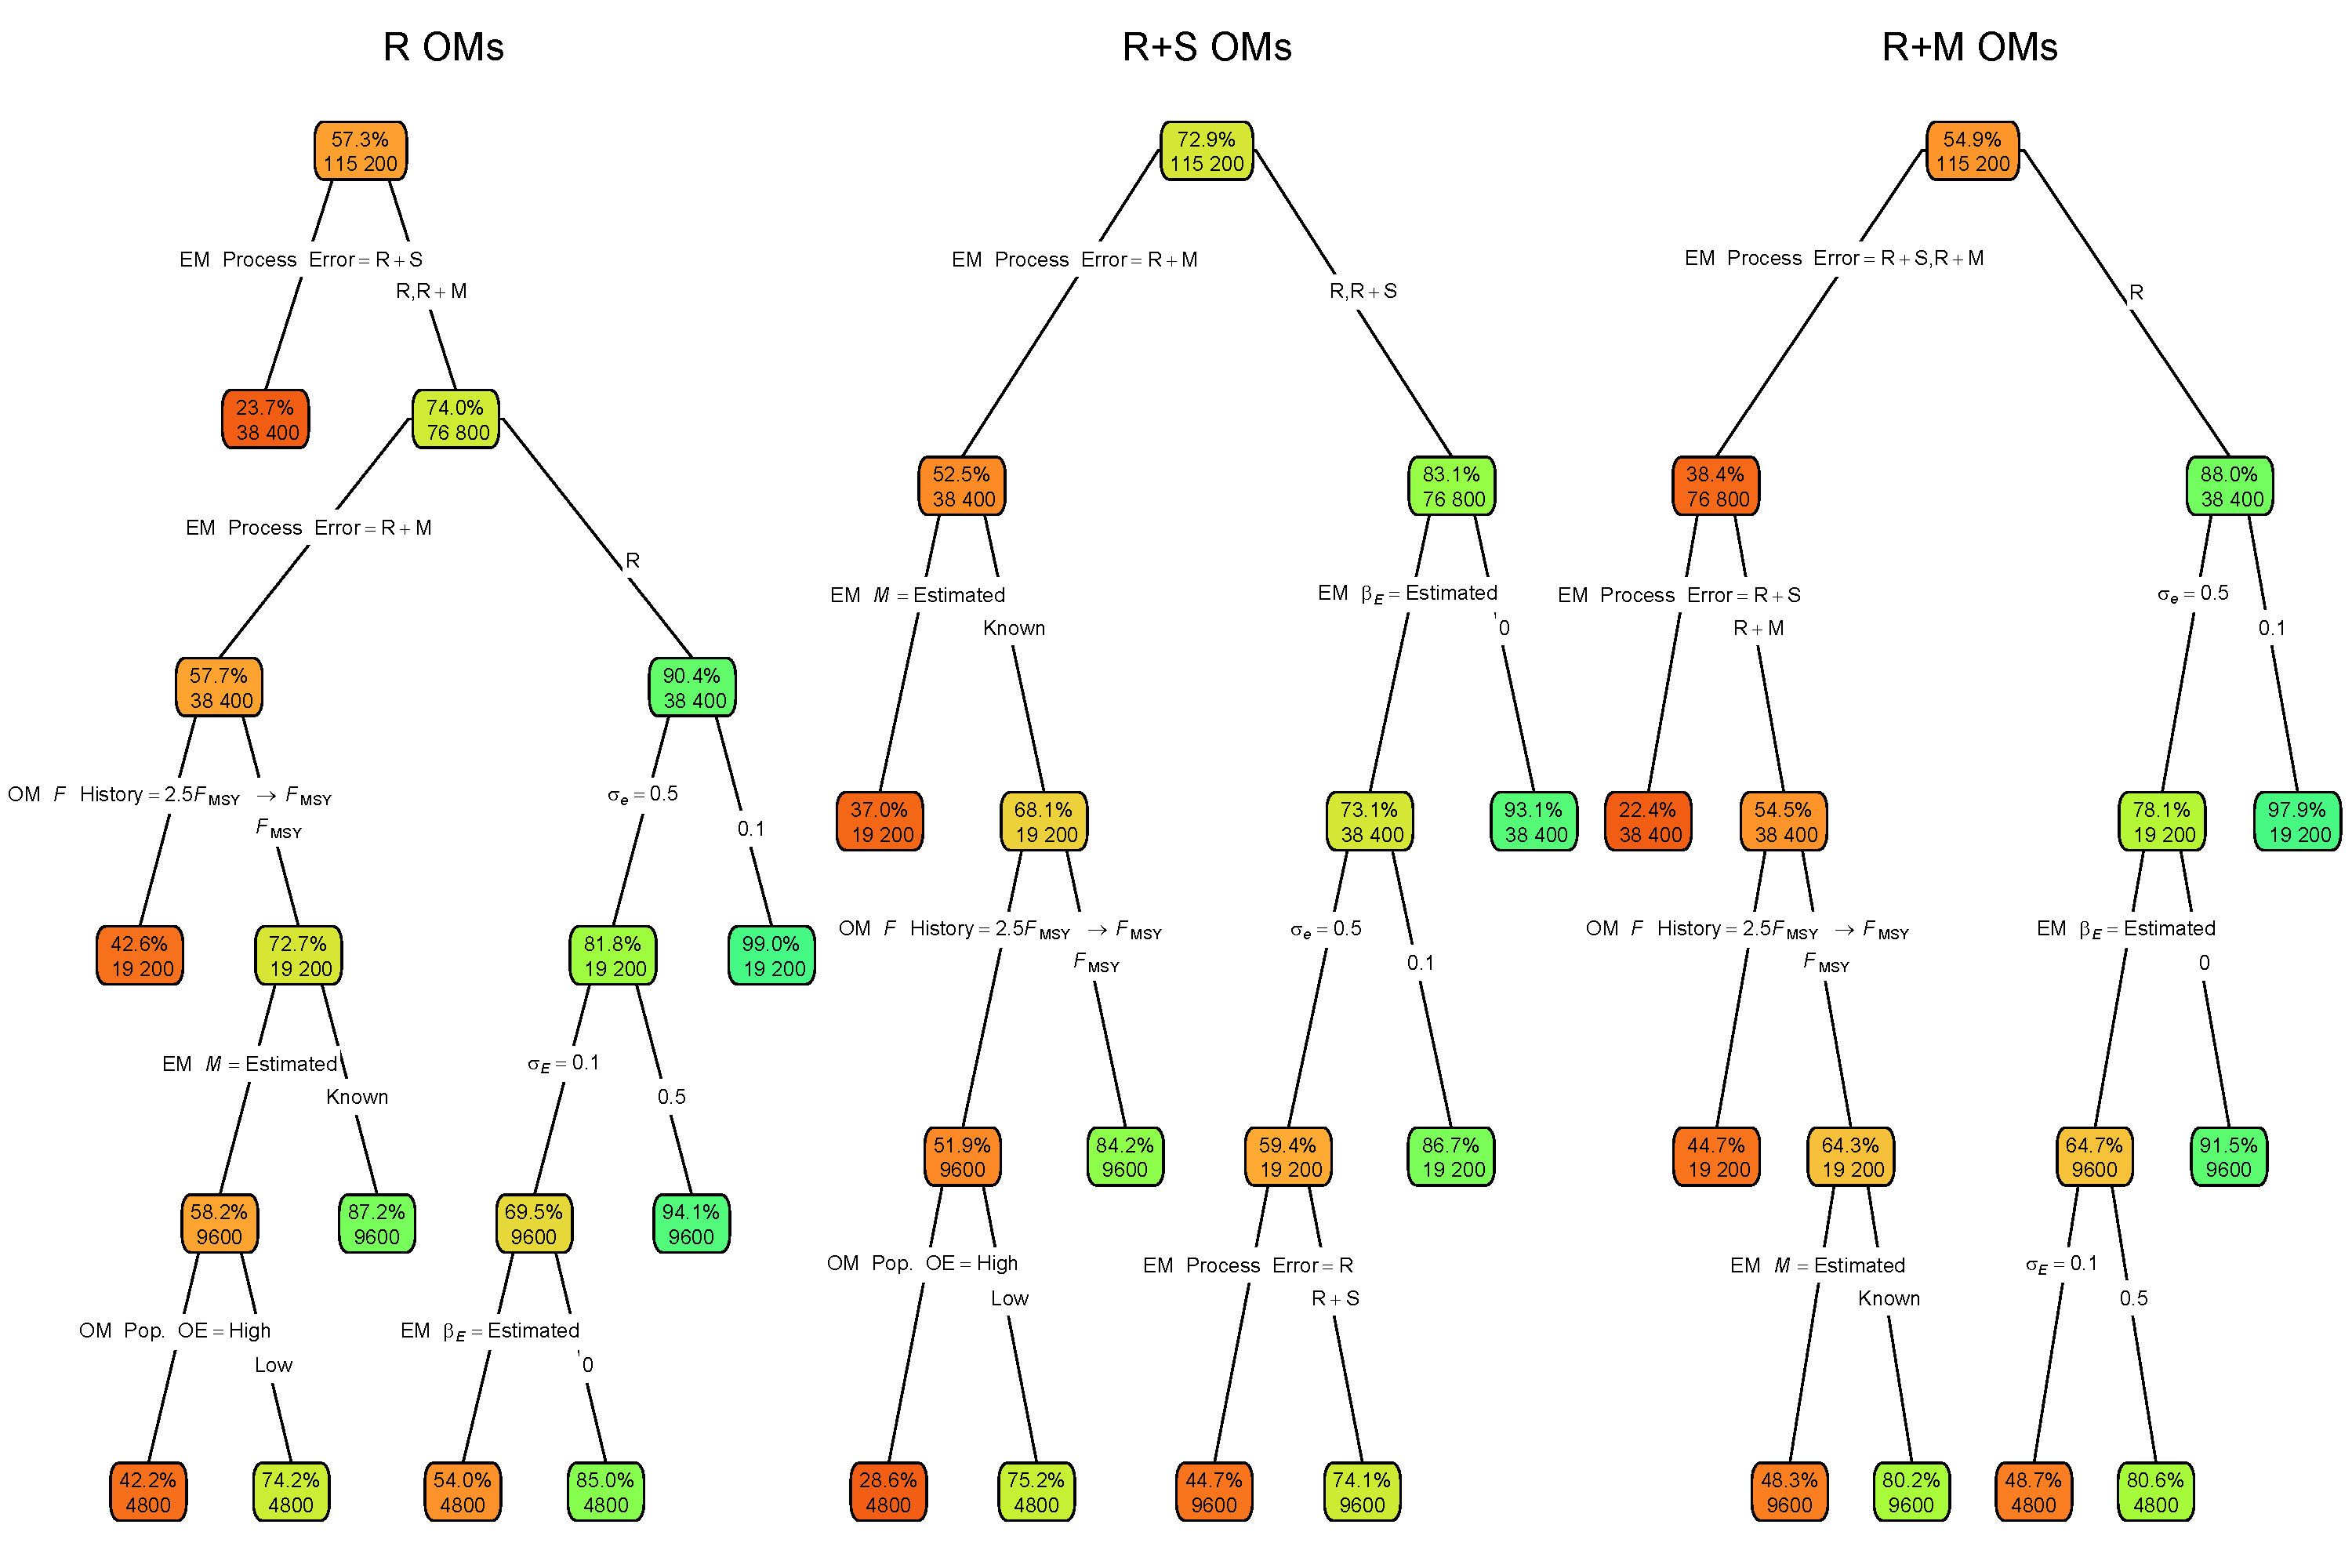
\includegraphics[width = 1.4\textwidth]{convergence_classification_plots}
\end{center}
\caption{Classification trees indicating primary factors determining convergence as defined by providing Hessian-based standard errors for operating models (OMs) with process error on recruitment only (R), recruitment and apparent survival (R+S), or recruitment and natural mortality (R+M). Nodes denote percent convergence (top) and number of fits (bottom) for the corresponding subset. Lower or higher convergence rates are indicated by more red or green polygons, respectively. See Table \ref{factor_table} for description of OM and \DIFaddbeginFL \DIFaddFL{estimating model (}\DIFaddendFL EM\DIFaddbeginFL \DIFaddFL{) }\DIFaddendFL factors defining nodes and branches.}\label{conv_class}
\end{figure}
\end{landscape}

\begin{landscape}
\begin{figure}
\begin{center}
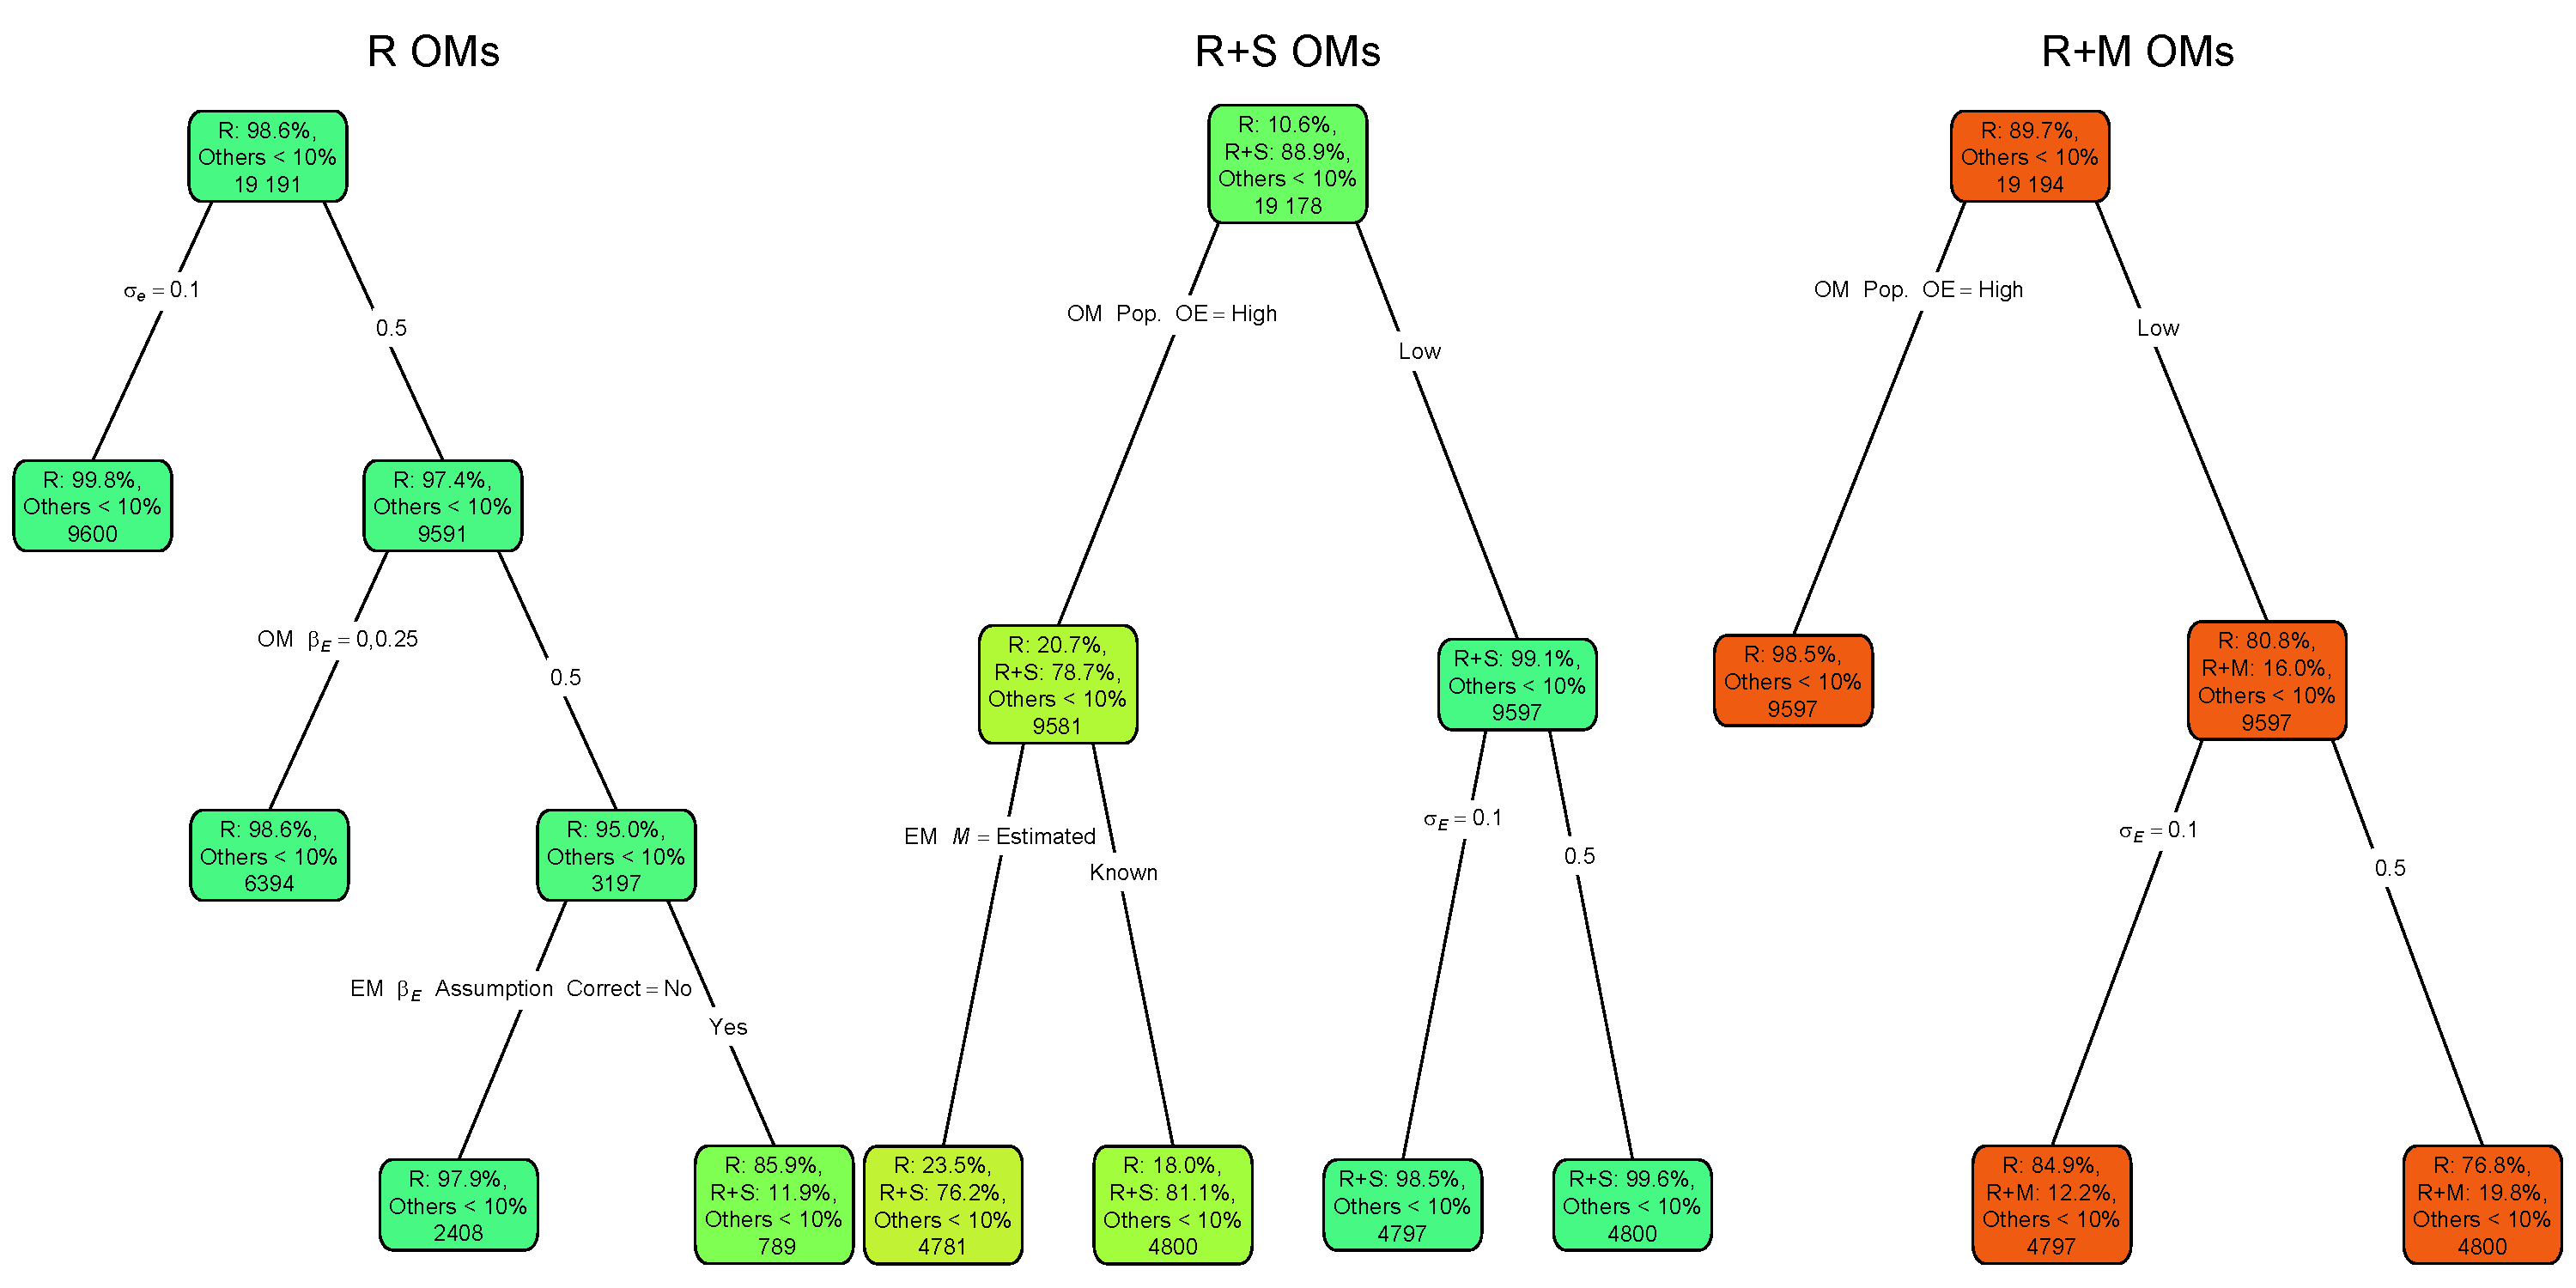
\includegraphics[width = 1.4\textwidth]{AIC_PE_classification_plots}
\end{center}
\caption{Classification trees \DIFdelbeginFL \DIFdelFL{indicating primary factors determining }\DIFdelendFL \DIFaddbeginFL \DIFaddFL{for }\DIFaddendFL which \DIFaddbeginFL \DIFaddFL{estimating model }\DIFaddendFL process error assumption \DIFdelbeginFL \DIFdelFL{in estimating models (EMs) }\DIFdelendFL provides the lowest AIC\DIFdelbeginFL \DIFdelFL{for operating models (OMs) with process error on recruitment only (R), recruitment and apparent survival (R+S), or recruitment and natural mortality (R+M)}\DIFdelendFL . Each node shows the \DIFdelbeginFL \DIFdelFL{percentage }\DIFdelendFL \DIFaddbeginFL \DIFaddFL{percentages (if greater than 10\%) }\DIFaddendFL of \DIFdelbeginFL \DIFdelFL{EM }\DIFdelendFL \DIFaddbeginFL \DIFaddFL{estimating model }\DIFaddendFL fits with a given process error assumption having the lowest AIC \DIFdelbeginFL \DIFdelFL{and the number of observations }\DIFdelendFL for the corresponding subset\DIFdelbeginFL \DIFdelFL{of fits}\DIFdelendFL . \DIFaddbeginFL \DIFaddFL{Process error assumptions with percentages less than 10\% are grouped as ``other.'' }\DIFaddendFL Lower or higher accuracy \DIFdelbeginFL \DIFdelFL{of the process error assumption }\DIFdelendFL are indicated by more red or green polygons, respectively. See \DIFaddbeginFL \DIFaddFL{Figure \ref{conv_class} caption and }\DIFaddendFL Table \ref{factor_table} for \DIFdelbeginFL \DIFdelFL{description of OM and EM factors defining nodes and branches}\DIFdelendFL \DIFaddbeginFL \DIFaddFL{further details}\DIFaddendFL .}\label{AIC_PE_class}
\end{figure}
\end{landscape}

\begin{landscape}
\begin{figure}
\begin{center}
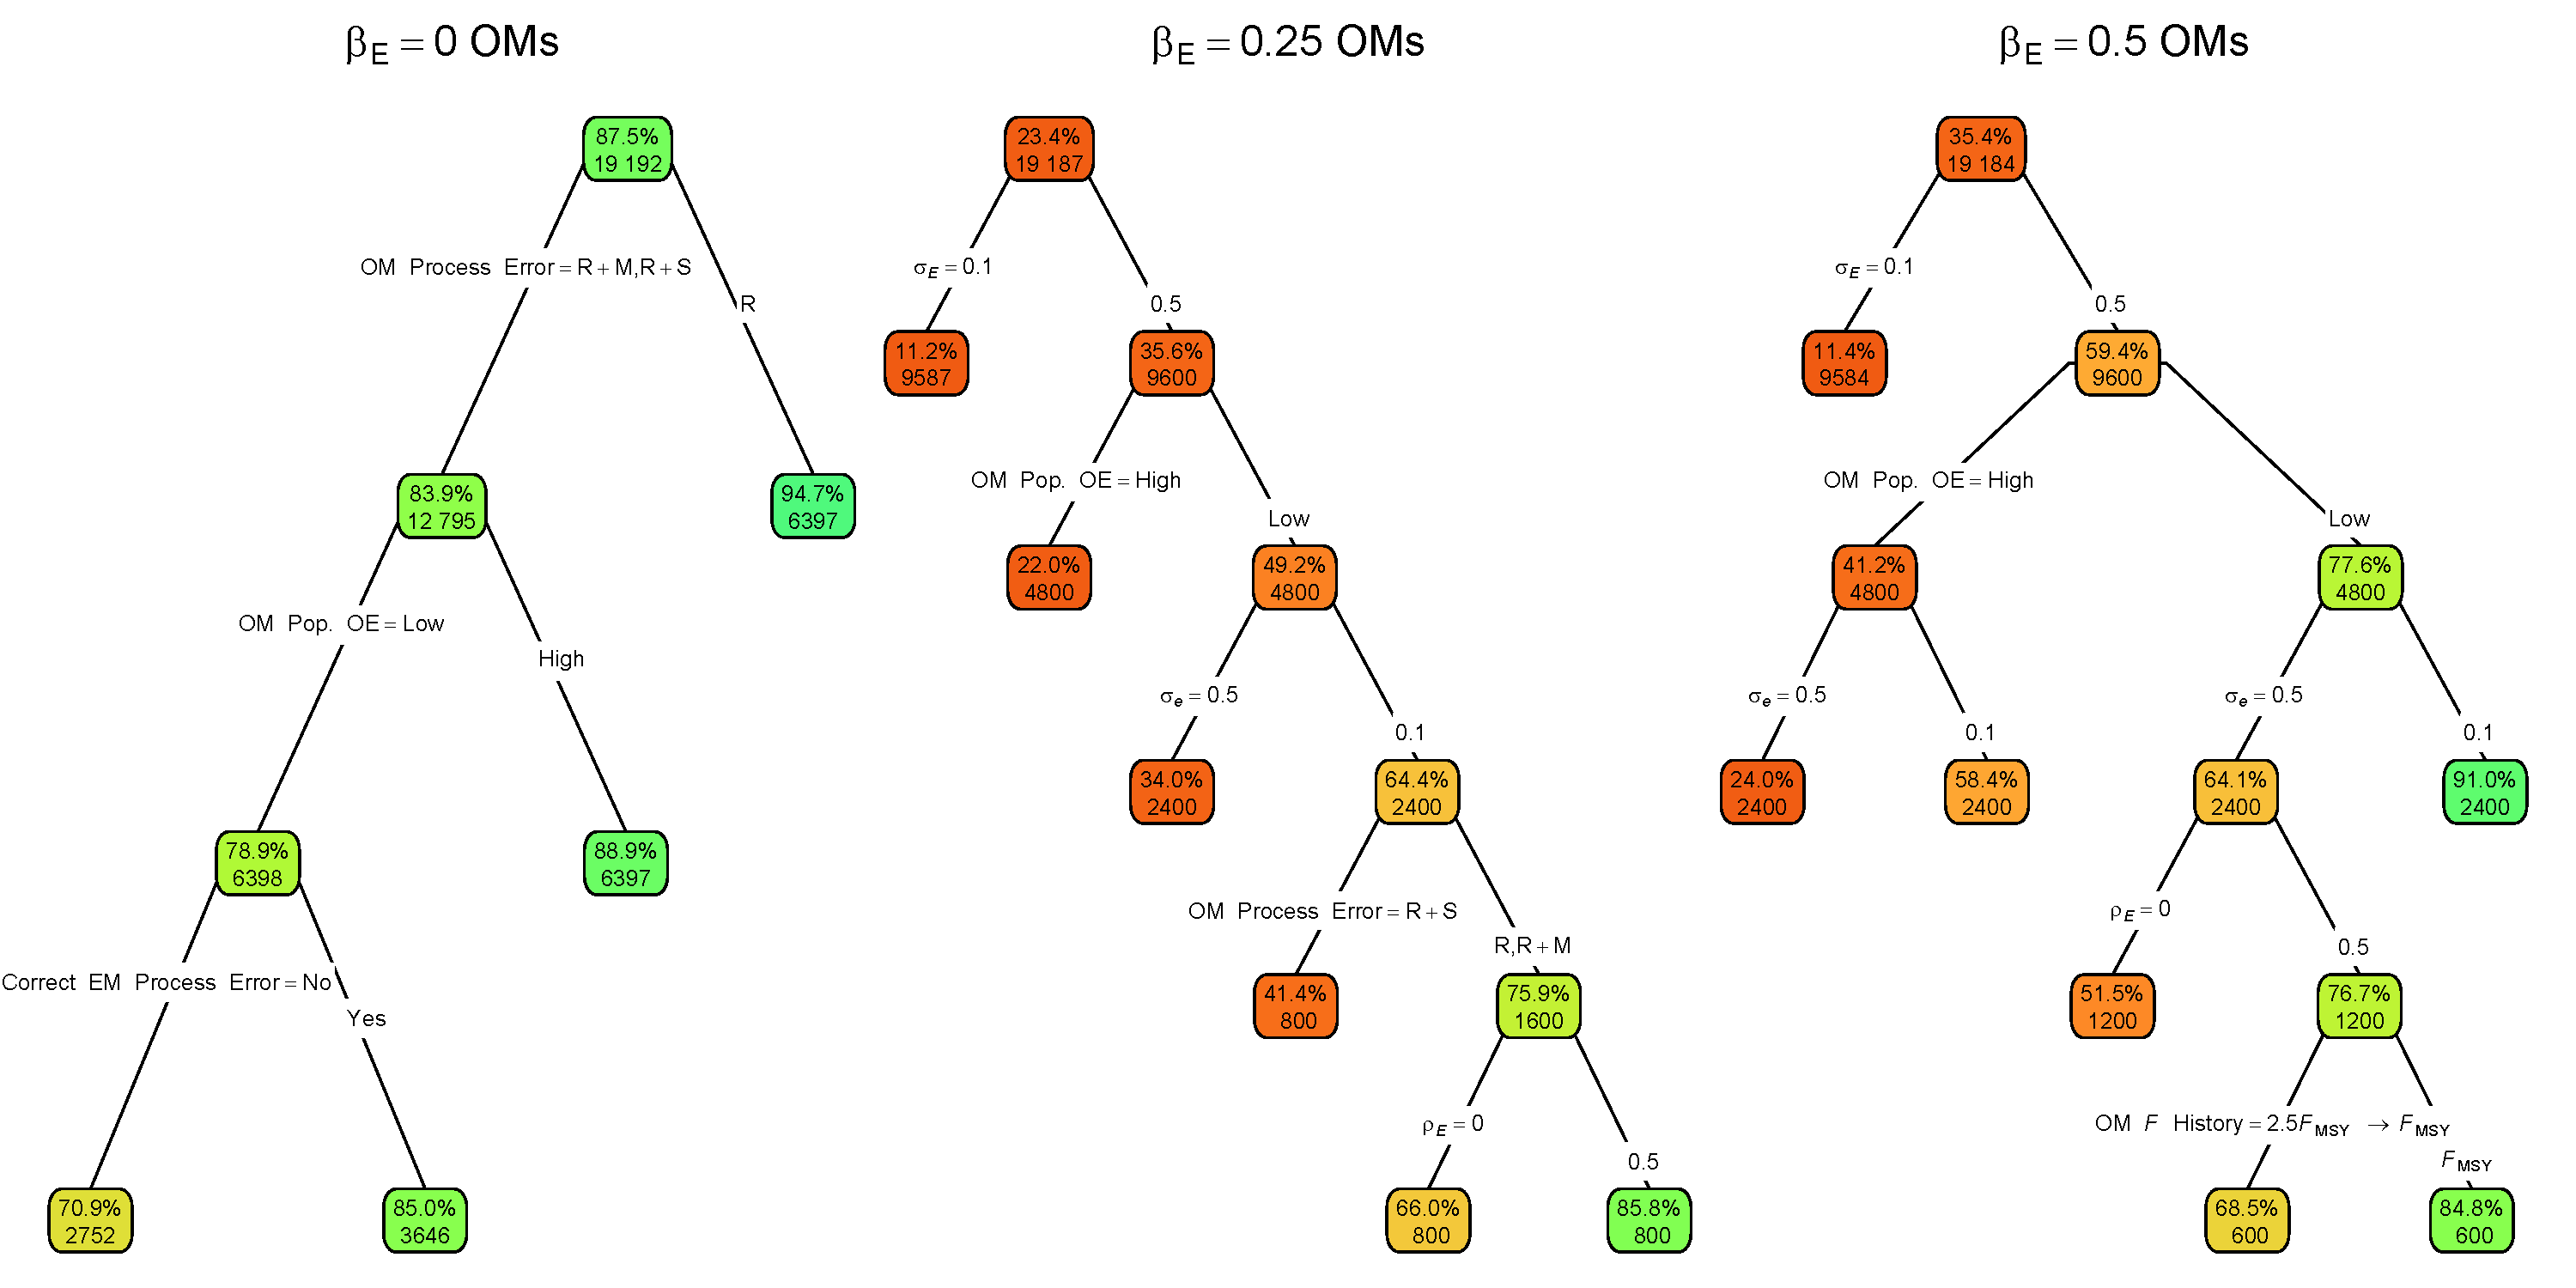
\includegraphics[width = 1.4\textwidth]{AIC_Ecov_effect_classification_plots}
\end{center}
\caption{Classification trees \DIFdelbeginFL \DIFdelFL{indicating primary factors determining }\DIFdelendFL \DIFaddbeginFL \DIFaddFL{for }\DIFaddendFL whether the correct \DIFdelbeginFL \DIFdelFL{EM }\DIFdelendFL \DIFaddbeginFL \DIFaddFL{estimating model }\DIFaddendFL assumption for covariate effect on $M$ (no effect with OM $\beta_E = 0$ or estimated effect when OM $\beta_E > 0$) provides the lowest AIC for OMs assuming values for $\beta_E$ of 0, 0.25, and 0.5. Nodes denote the percentage of estimating models \DIFdelbeginFL \DIFdelFL{(EMs) }\DIFdelendFL with \DIFaddbeginFL \DIFaddFL{the }\DIFaddendFL correct assumption and lowest AIC  \DIFdelbeginFL \DIFdelFL{(top), and number of observations (bottom) }\DIFdelendFL for the corresponding subset. Lower or higher accuracy \DIFdelbeginFL \DIFdelFL{of the process error assumption }\DIFdelendFL are indicated by more red or green polygons, respectively. See \DIFaddbeginFL \DIFaddFL{Figure \ref{conv_class} caption and }\DIFaddendFL Table \ref{factor_table} for \DIFdelbeginFL \DIFdelFL{description of OM and EM factors defining nodes and branches}\DIFdelendFL \DIFaddbeginFL \DIFaddFL{further details}\DIFaddendFL .}\label{AIC_Ecov_effect_class}
\end{figure}
\end{landscape}

\begin{landscape}
\begin{figure}
\begin{center}
\DIFdelbeginFL %DIFDELCMD < 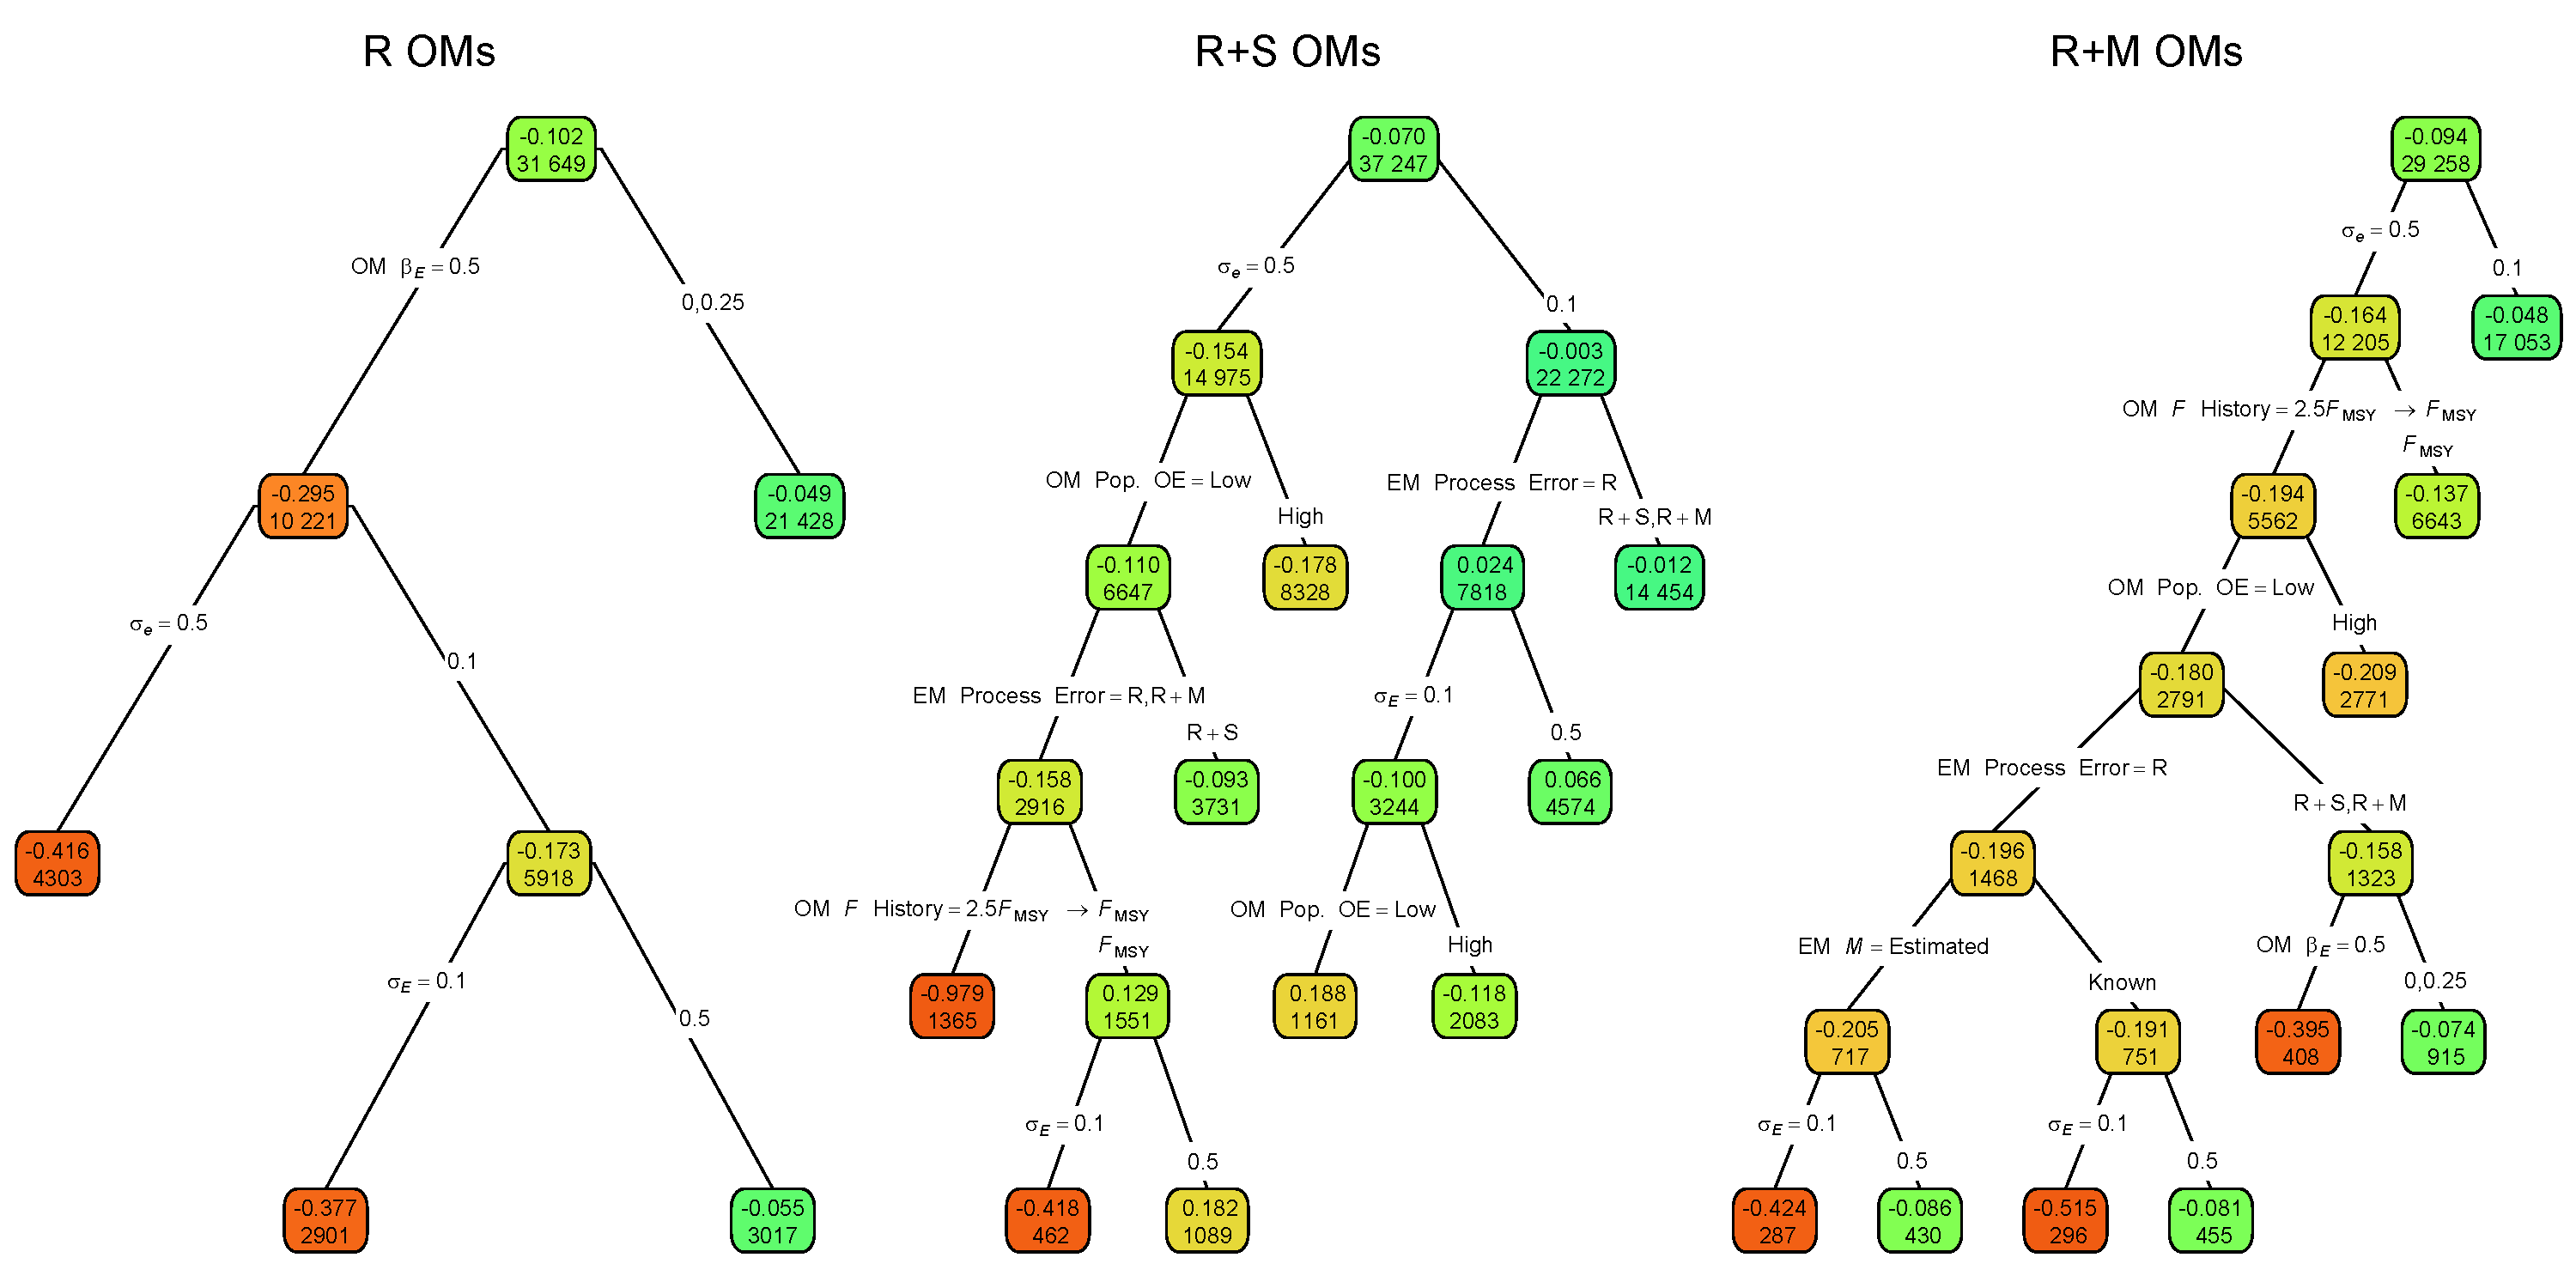
\includegraphics[width = 1.4\textwidth]{ecov_beta_bias_regtree_plots}
%DIFDELCMD < %%%
\DIFdelendFL \DIFaddbeginFL 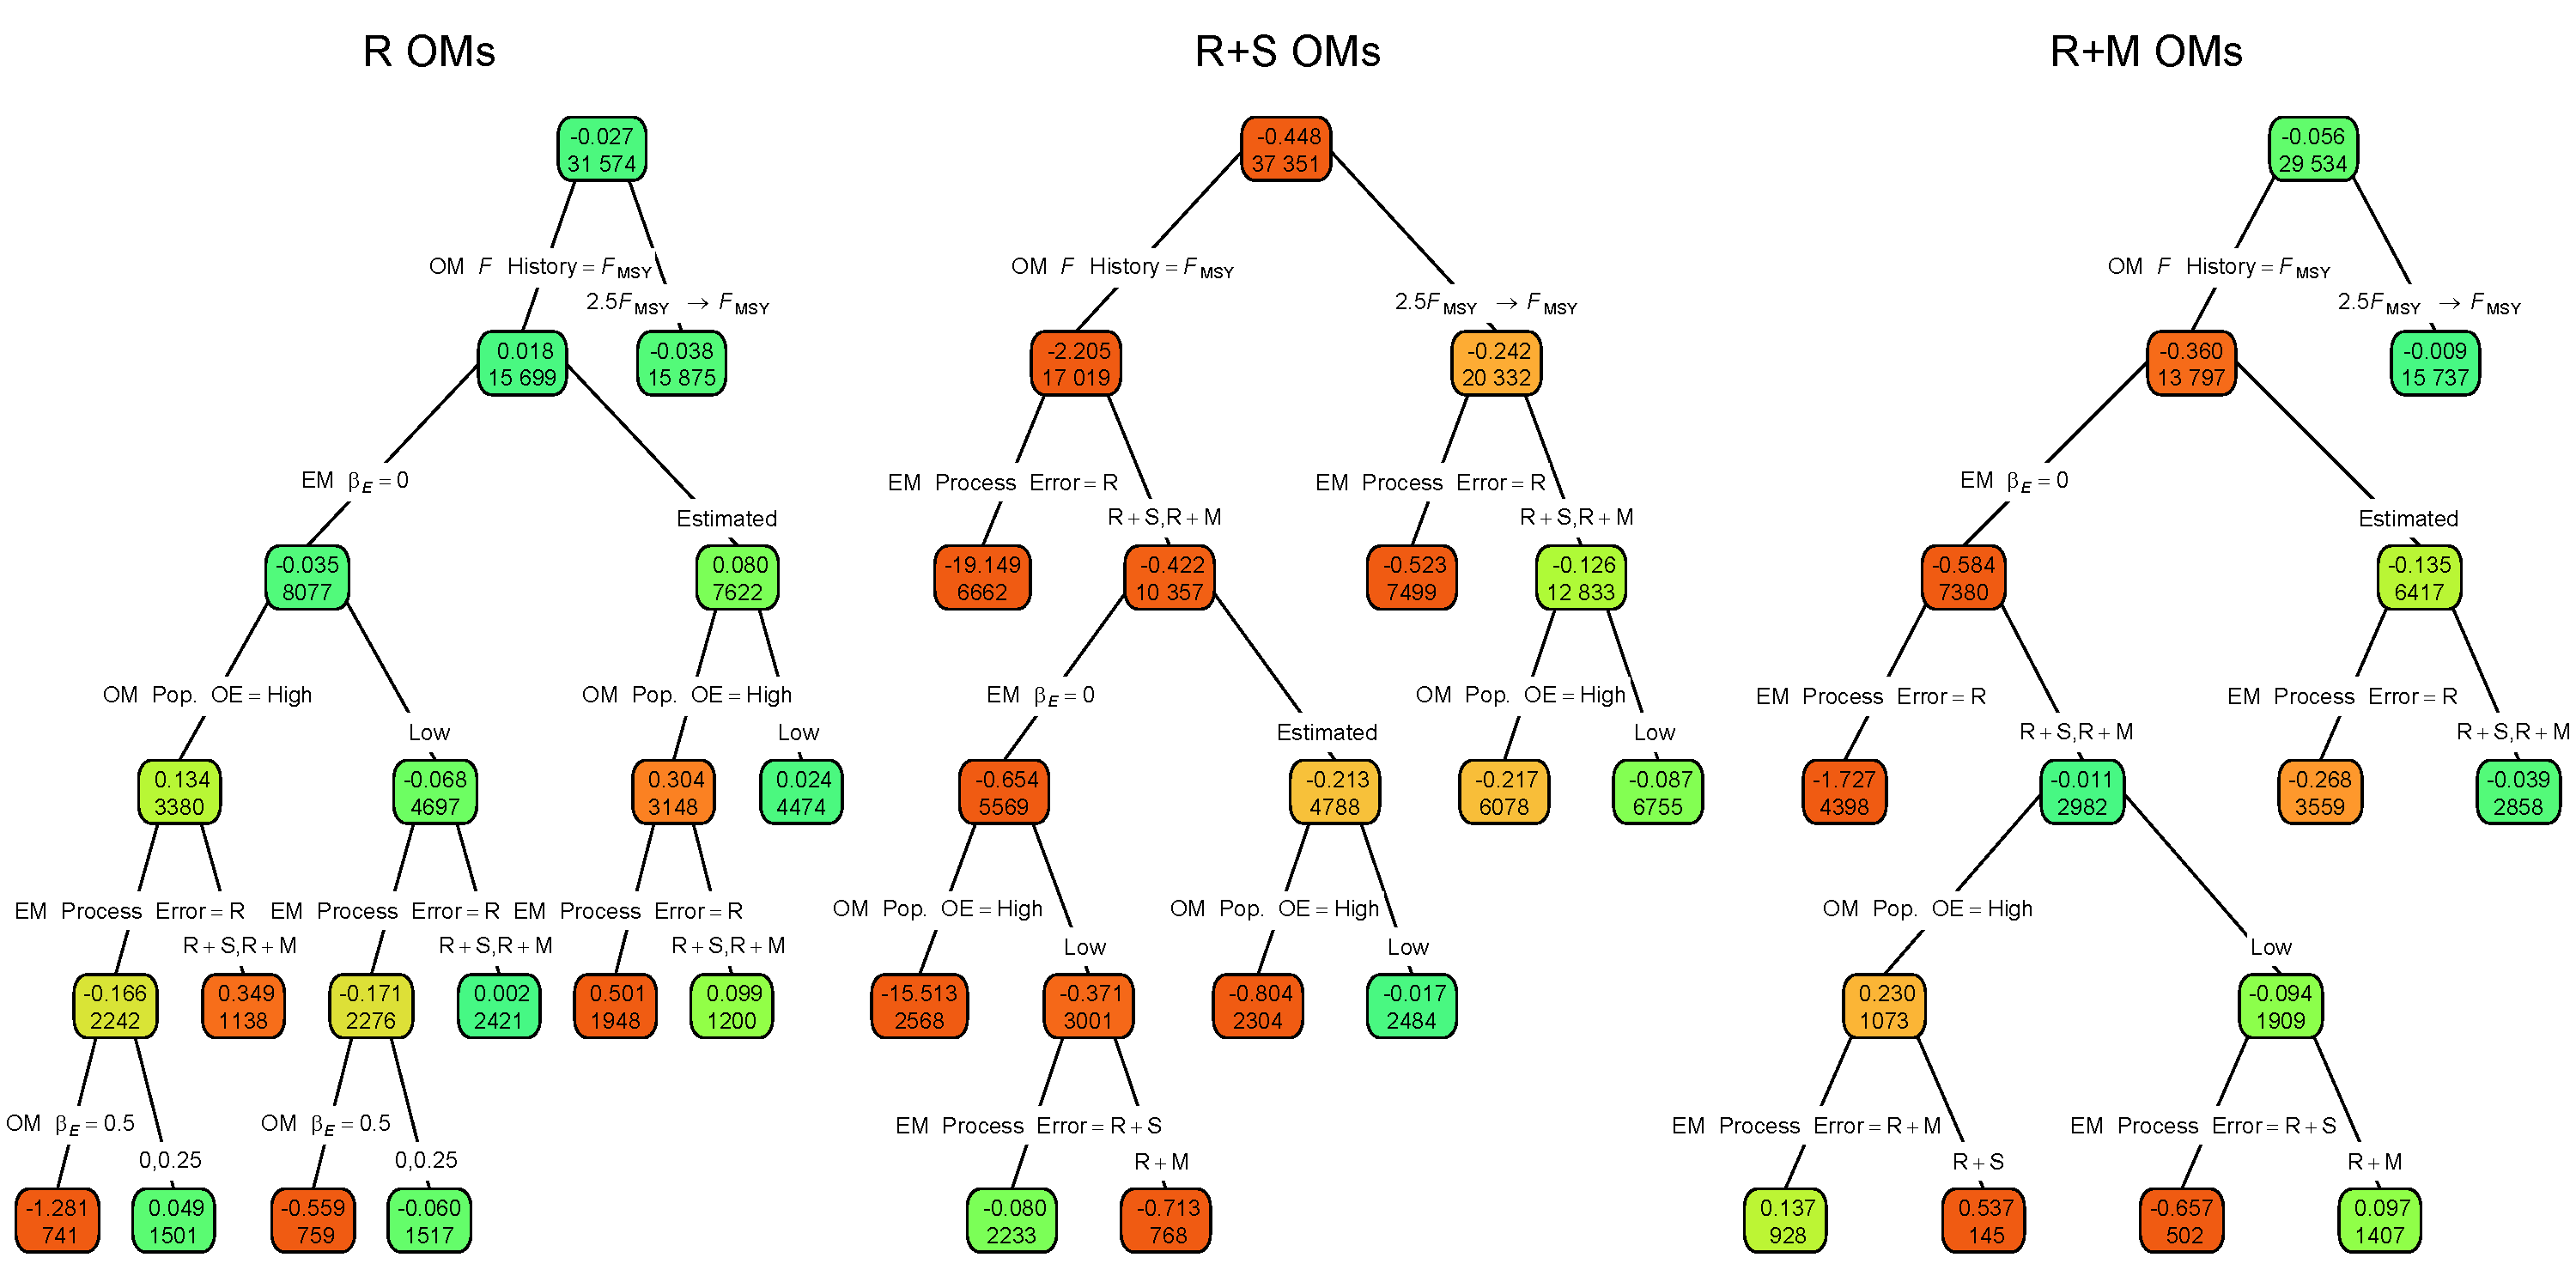
\includegraphics[width = 1.4\textwidth]{median_M_bias_regtree_plots}
\DIFaddendFL \end{center}
\caption{Regression trees \DIFdelbeginFL \DIFdelFL{indicating primary factors determining reductions in sums of squares of errors in }\DIFdelendFL \DIFaddbeginFL \DIFaddFL{for }\DIFaddendFL estimation \DIFaddbeginFL \DIFaddFL{error }\DIFaddendFL of the \DIFdelbeginFL \DIFdelFL{covariate effect on }\DIFdelendFL \DIFaddbeginFL \DIFaddFL{median }\DIFaddendFL $M$ \DIFdelbeginFL \DIFdelFL{for operating models }\DIFdelendFL \DIFaddbeginFL \DIFaddFL{parameter }\DIFaddendFL (\DIFdelbeginFL \DIFdelFL{OMs}\DIFdelendFL \DIFaddbeginFL \DIFaddFL{$\beta_M$}\DIFaddendFL )\DIFdelbeginFL \DIFdelFL{with process error on recruitment only (R), recruitment and apparent survival (R+S), or recruitment and natural mortality (R+M)}\DIFdelendFL . Each node shows the median error \DIFdelbeginFL \DIFdelFL{(top) and number of observations (bottom) }\DIFdelendFL for the corresponding subset. Lower or higher \DIFdelbeginFL \DIFdelFL{median }\DIFdelendFL absolute \DIFaddbeginFL \DIFaddFL{median }\DIFaddendFL errors \DIFdelbeginFL \DIFdelFL{of the process error assumption }\DIFdelendFL are indicated by more green or red polygons, respectively. See \DIFaddbeginFL \DIFaddFL{Figure \ref{conv_class} caption and }\DIFaddendFL Table \ref{factor_table} for \DIFdelbeginFL \DIFdelFL{description of OM and EM factors defining nodes and branches}\DIFdelendFL \DIFaddbeginFL \DIFaddFL{further details}\DIFaddendFL .}\DIFdelbeginFL %DIFDELCMD < \label{ecov_effect_bias_regtree}
%DIFDELCMD < %%%
\DIFdelendFL \DIFaddbeginFL \label{med_M_bias_regtree}
\DIFaddendFL \end{figure}
\end{landscape}

\begin{landscape}
\begin{figure}
\begin{center}
\DIFdelbeginFL %DIFDELCMD < 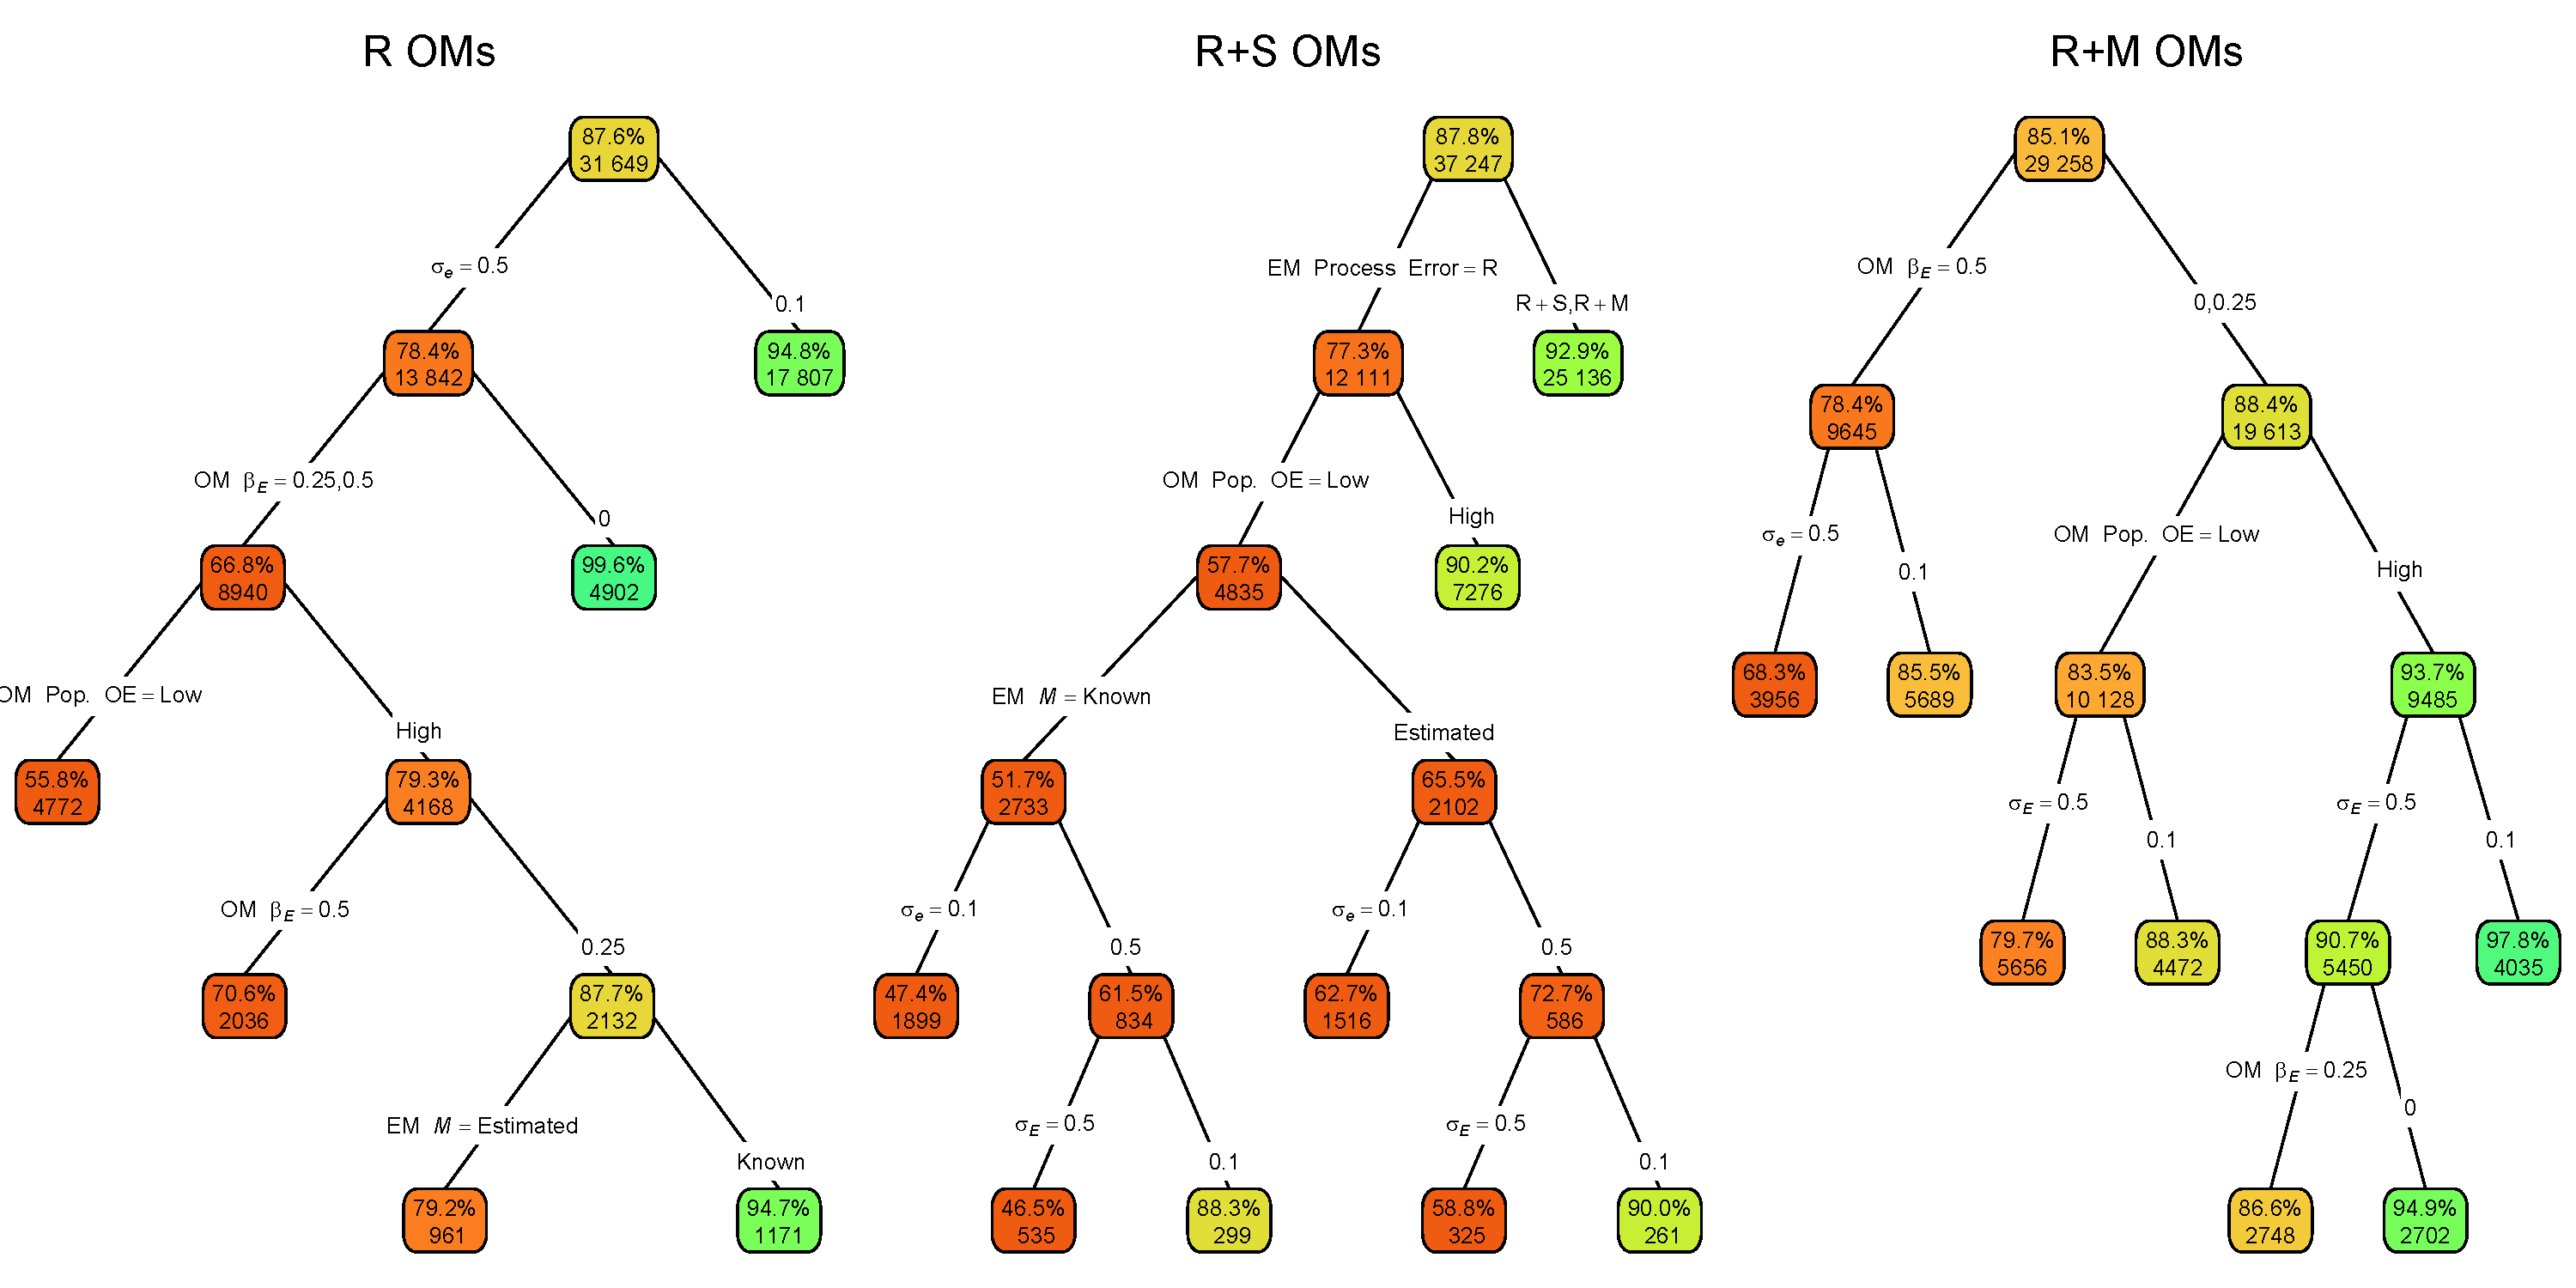
\includegraphics[width = 1.4\textwidth]{ecov_beta_CI_coverage_regtree_plots}
%DIFDELCMD < %%%
\DIFdelendFL \DIFaddbeginFL 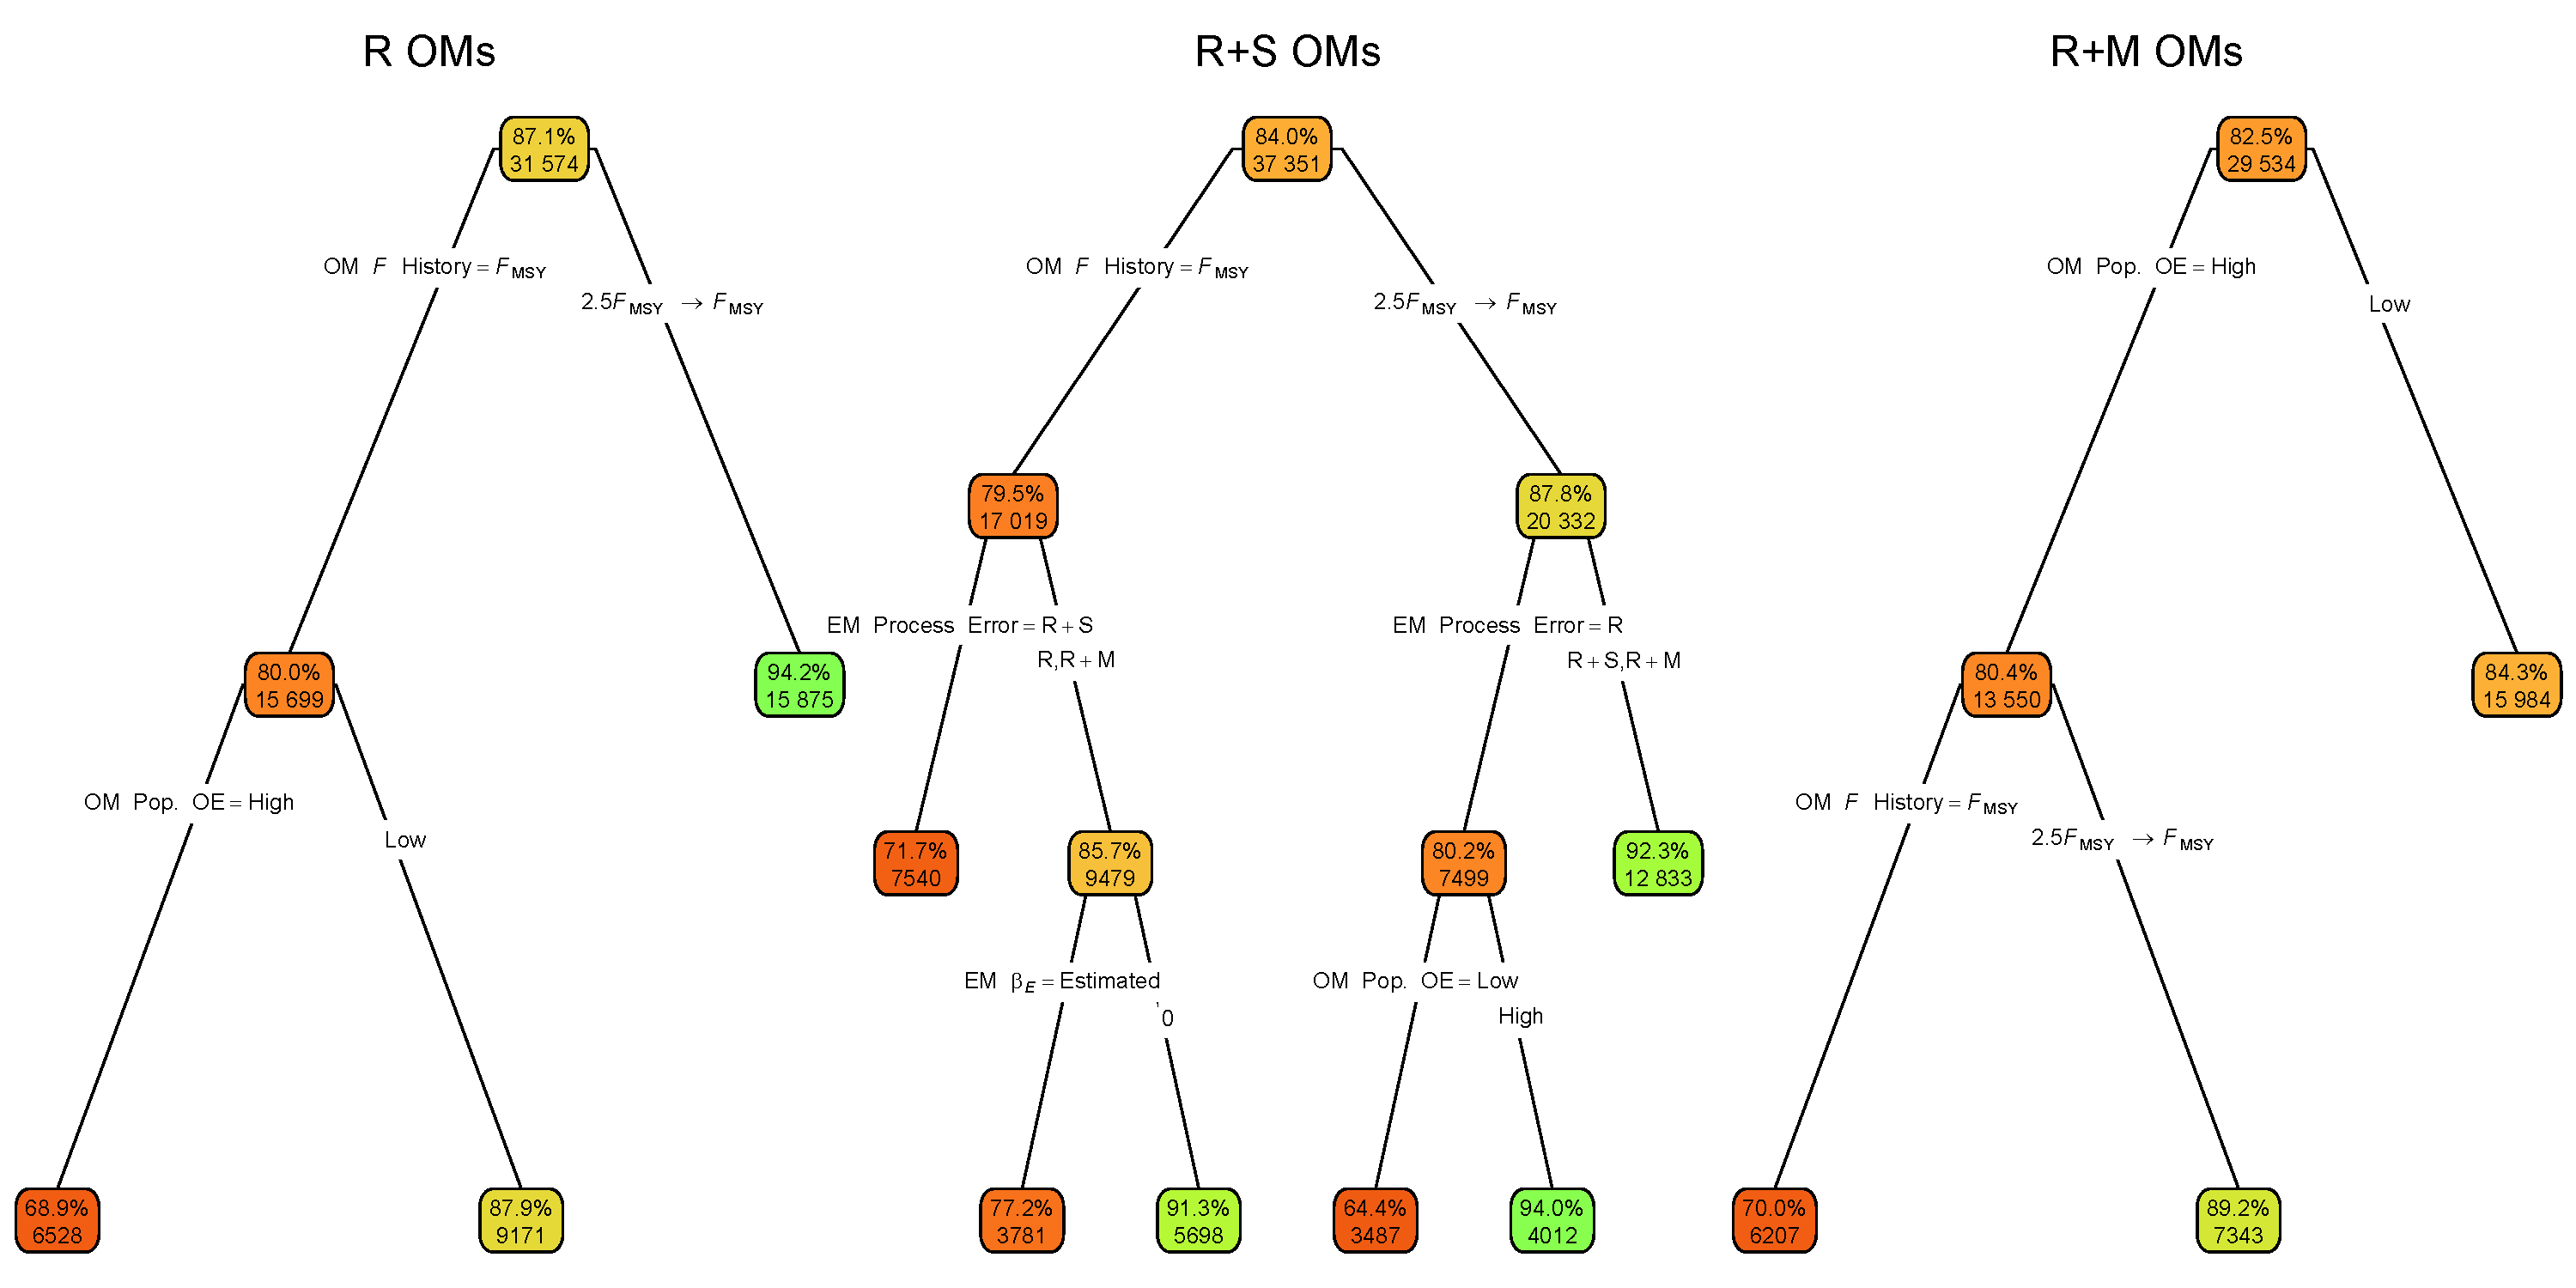
\includegraphics[width = 1.4\textwidth]{median_M_CI_coverage_regtree_plots}
\DIFaddendFL \end{center}
\caption{Classification trees \DIFdelbeginFL \DIFdelFL{indicating primary factors determining }\DIFdelendFL \DIFaddbeginFL \DIFaddFL{for }\DIFaddendFL whether confidence intervals \DIFaddbeginFL \DIFaddFL{(CIs) }\DIFaddendFL for \DIFaddbeginFL \DIFaddFL{the }\DIFaddendFL estimated \DIFdelbeginFL \DIFdelFL{covariate effects on }\DIFdelendFL \DIFaddbeginFL \DIFaddFL{median }\DIFaddendFL $M$ \DIFdelbeginFL \DIFdelFL{in estimating models }\DIFdelendFL \DIFaddbeginFL \DIFaddFL{parameter }\DIFaddendFL (\DIFdelbeginFL \DIFdelFL{EMs}\DIFdelendFL \DIFaddbeginFL \DIFaddFL{$\beta_M$}\DIFaddendFL ) \DIFdelbeginFL \DIFdelFL{fitted to operating models (OMs) with process error on recruitment only (R), recruitment and apparent survival (R+S), or recruitment and natural mortality (R+M) }\DIFdelendFL included the true value. Each node shows the \DIFdelbeginFL \DIFdelFL{median error (top) and number }\DIFdelendFL \DIFaddbeginFL \DIFaddFL{percentage }\DIFaddendFL of \DIFdelbeginFL \DIFdelFL{observations (bottom) }\DIFdelendFL \DIFaddbeginFL \DIFaddFL{CIs that include the true value }\DIFaddendFL for the corresponding subset. \DIFdelbeginFL \DIFdelFL{Lower }\DIFdelendFL \DIFaddbeginFL \DIFaddFL{Higher }\DIFaddendFL or \DIFdelbeginFL \DIFdelFL{higher median absolute errors of the process error assumption }\DIFdelendFL \DIFaddbeginFL \DIFaddFL{lower percentages }\DIFaddendFL are indicated by more green or red polygons, respectively. See \DIFaddbeginFL \DIFaddFL{Figure \ref{conv_class} caption and }\DIFaddendFL Table \ref{factor_table} for \DIFdelbeginFL \DIFdelFL{description of OM and EM factors defining nodes and branches}\DIFdelendFL \DIFaddbeginFL \DIFaddFL{further details}\DIFaddendFL .}\DIFdelbeginFL %DIFDELCMD < \label{ecov_effect_CI_coverage_regtree}
%DIFDELCMD < %%%
\DIFdelendFL \DIFaddbeginFL \label{med_M_CI_coverage_regtree}
\DIFaddendFL \end{figure}
\end{landscape}

\begin{landscape}
\begin{figure}
\begin{center}
\DIFdelbeginFL %DIFDELCMD < 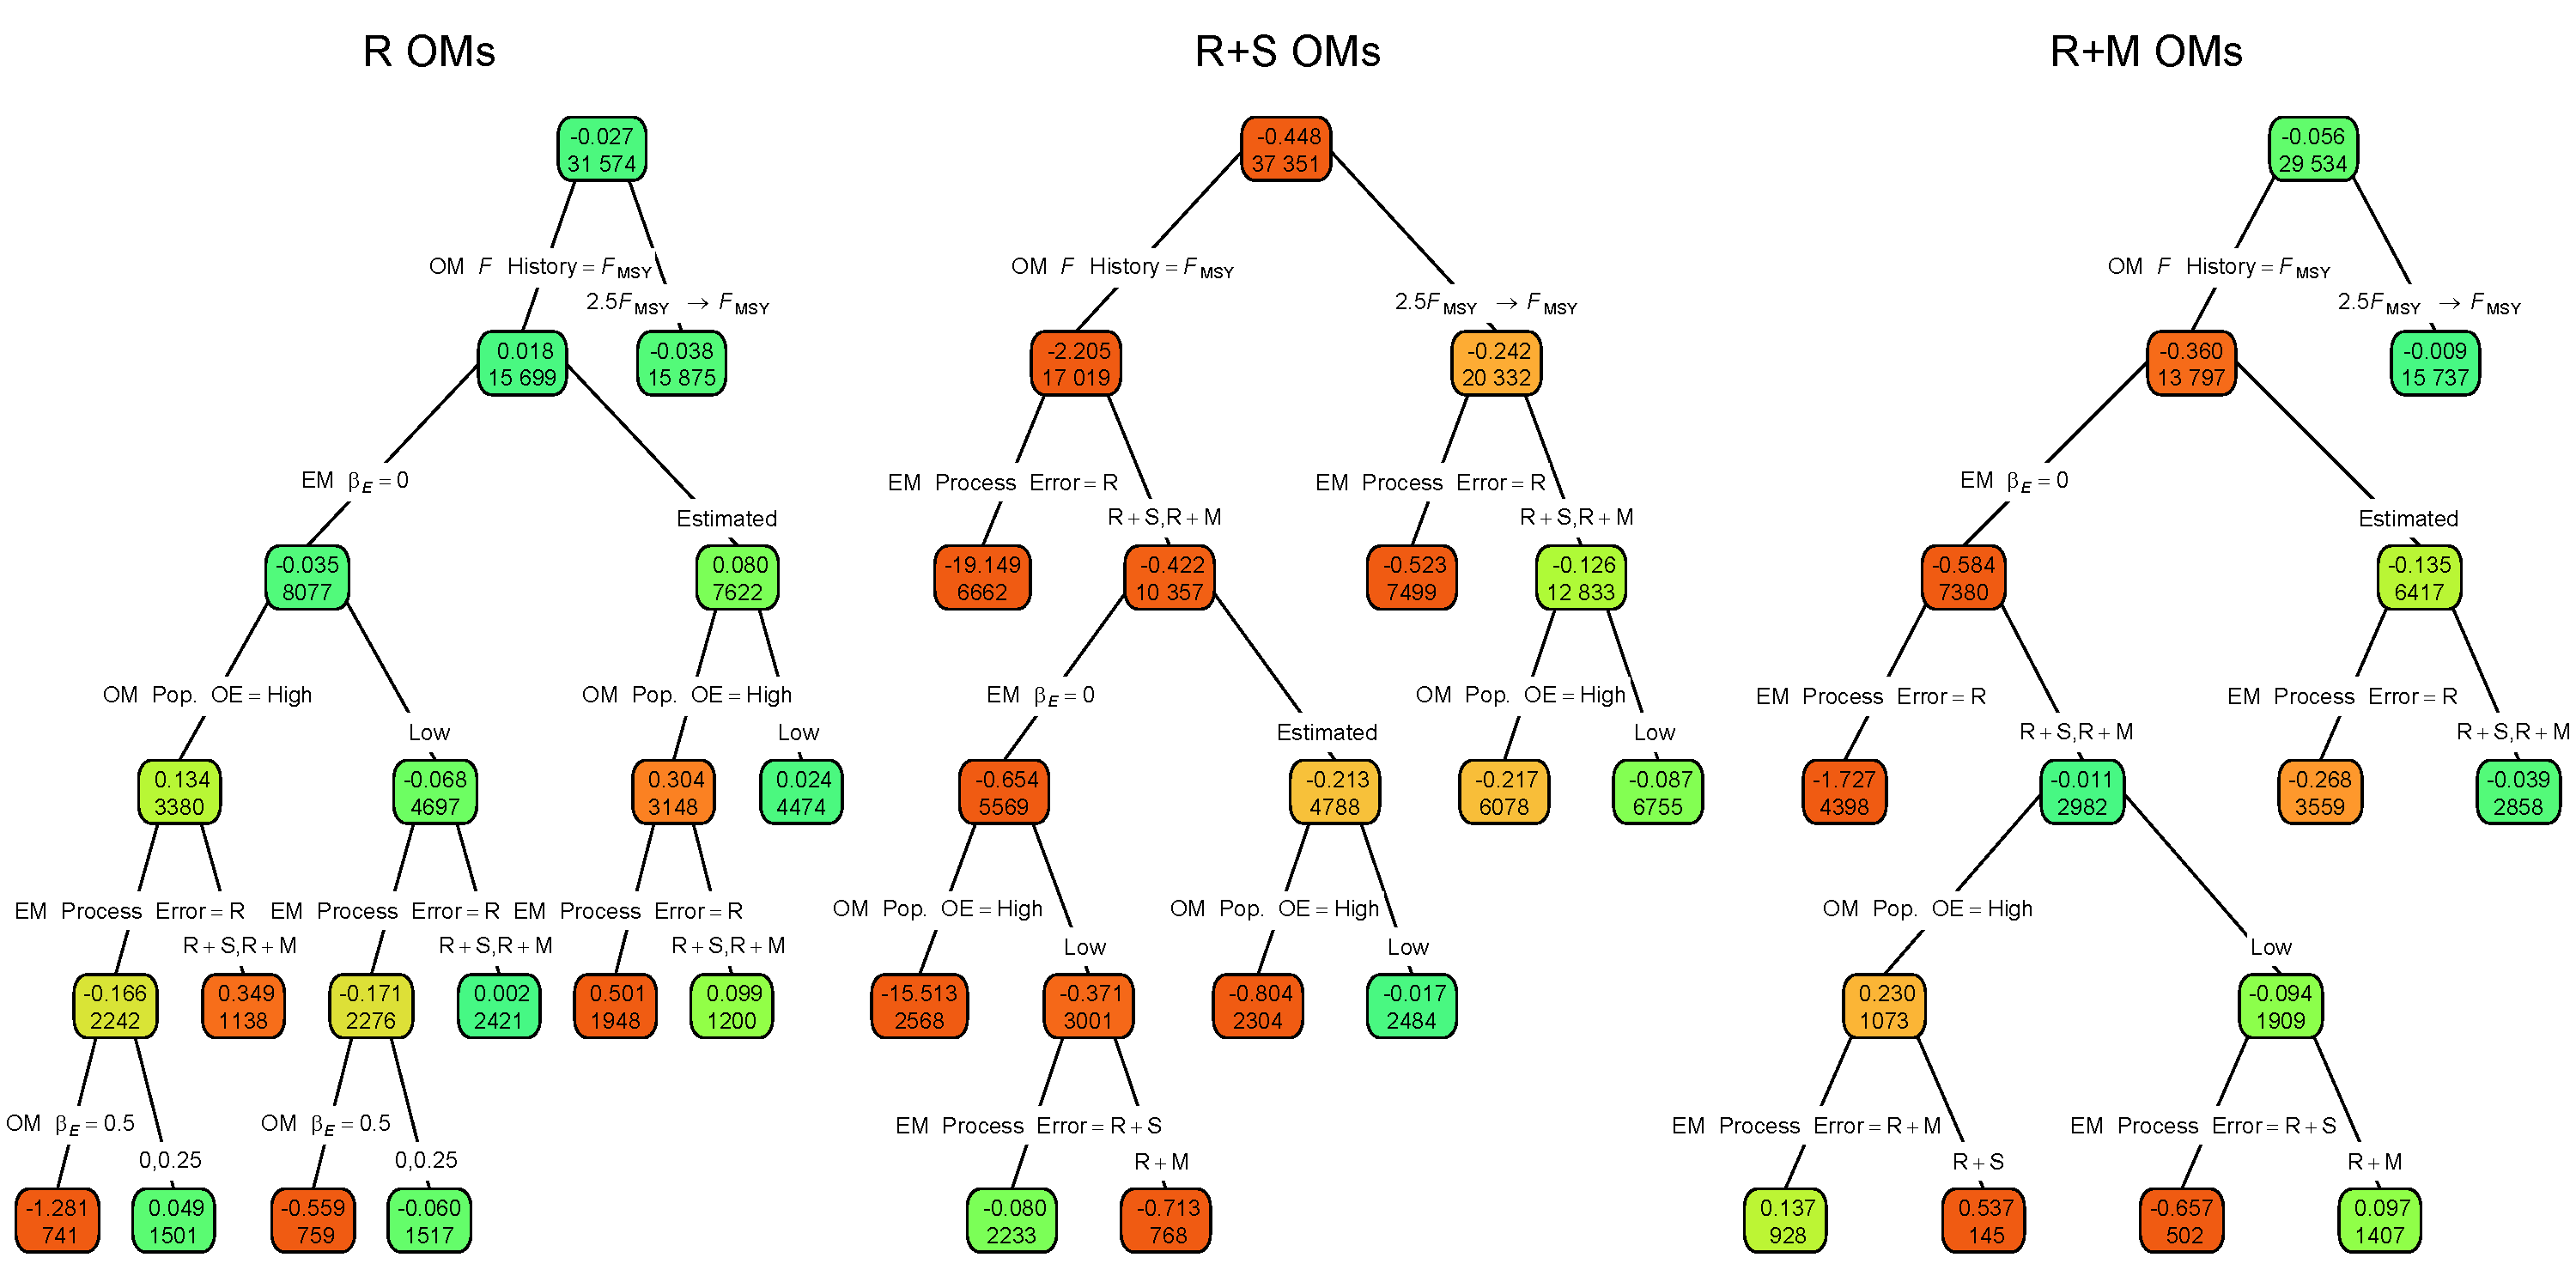
\includegraphics[width = 1.4\textwidth]{median_M_bias_regtree_plots}
%DIFDELCMD < %%%
\DIFdelendFL \DIFaddbeginFL 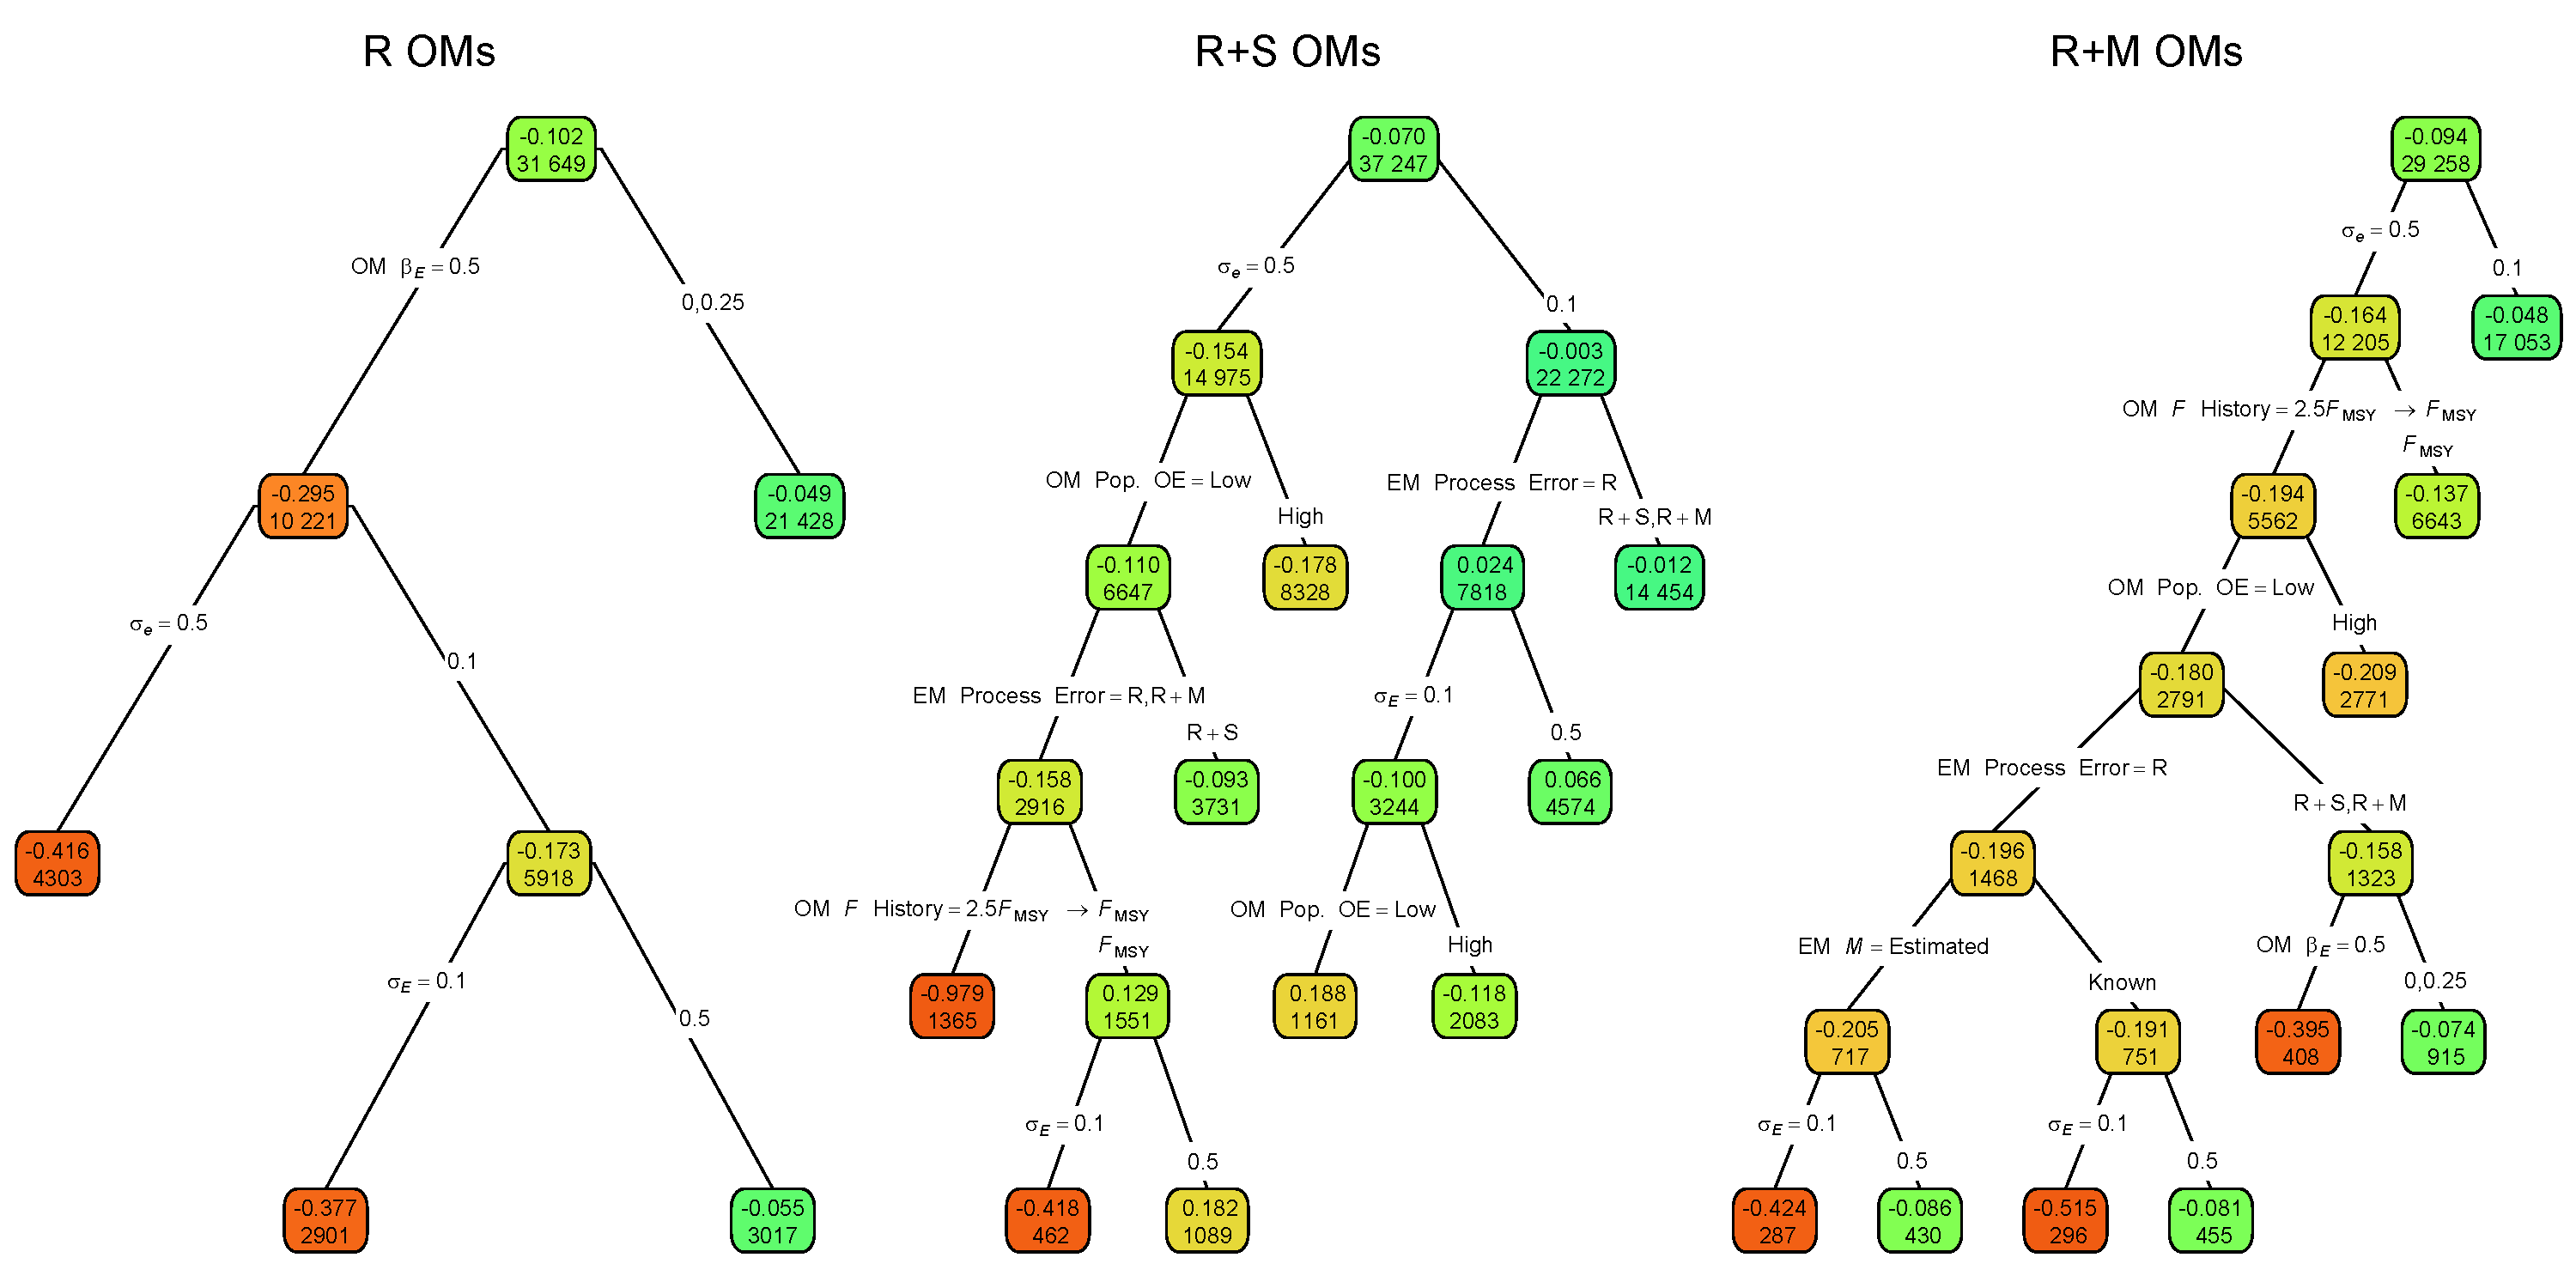
\includegraphics[width = 1.4\textwidth]{ecov_beta_bias_regtree_plots}
\DIFaddendFL \end{center}
\caption{Regression trees \DIFdelbeginFL \DIFdelFL{indicating primary factors determining reductions in sums of squares of errors in }\DIFdelendFL \DIFaddbeginFL \DIFaddFL{for }\DIFaddendFL estimation \DIFaddbeginFL \DIFaddFL{error }\DIFaddendFL of the \DIFdelbeginFL \DIFdelFL{median }\DIFdelendFL \DIFaddbeginFL \DIFaddFL{covariate effect on }\DIFaddendFL $M$ \DIFdelbeginFL \DIFdelFL{parameter }\DIFdelendFL (\DIFdelbeginFL \DIFdelFL{$\beta_M$}\DIFdelendFL \DIFaddbeginFL \DIFaddFL{$\widehat \beta_E$}\DIFaddendFL )\DIFdelbeginFL \DIFdelFL{in estimating models (EMs) fitted to operating models (OMs) with process error on recruitment only (R), recruitment and apparent survival (R+S), or recruitment and natural mortality (R+M)}\DIFdelendFL . Each node shows the median error (top) \DIFdelbeginFL \DIFdelFL{and number of observations (bottom) }\DIFdelendFL for the corresponding subset. Lower or higher \DIFdelbeginFL \DIFdelFL{median }\DIFdelendFL absolute \DIFdelbeginFL \DIFdelFL{errors of the process }\DIFdelendFL \DIFaddbeginFL \DIFaddFL{median }\DIFaddendFL error \DIFdelbeginFL \DIFdelFL{assumption }\DIFdelendFL are indicated by more green or red polygons, respectively. See \DIFaddbeginFL \DIFaddFL{Figure \ref{conv_class} caption and }\DIFaddendFL Table \ref{factor_table} for \DIFdelbeginFL \DIFdelFL{description of OM and EM factors defining nodes and branches}\DIFdelendFL \DIFaddbeginFL \DIFaddFL{further details}\DIFaddendFL .}\DIFdelbeginFL %DIFDELCMD < \label{med_M_bias_regtree}
%DIFDELCMD < %%%
\DIFdelendFL \DIFaddbeginFL \label{ecov_effect_bias_regtree}
\DIFaddendFL \end{figure}
\end{landscape}

\begin{landscape}
\begin{figure}
\begin{center}
\DIFdelbeginFL %DIFDELCMD < 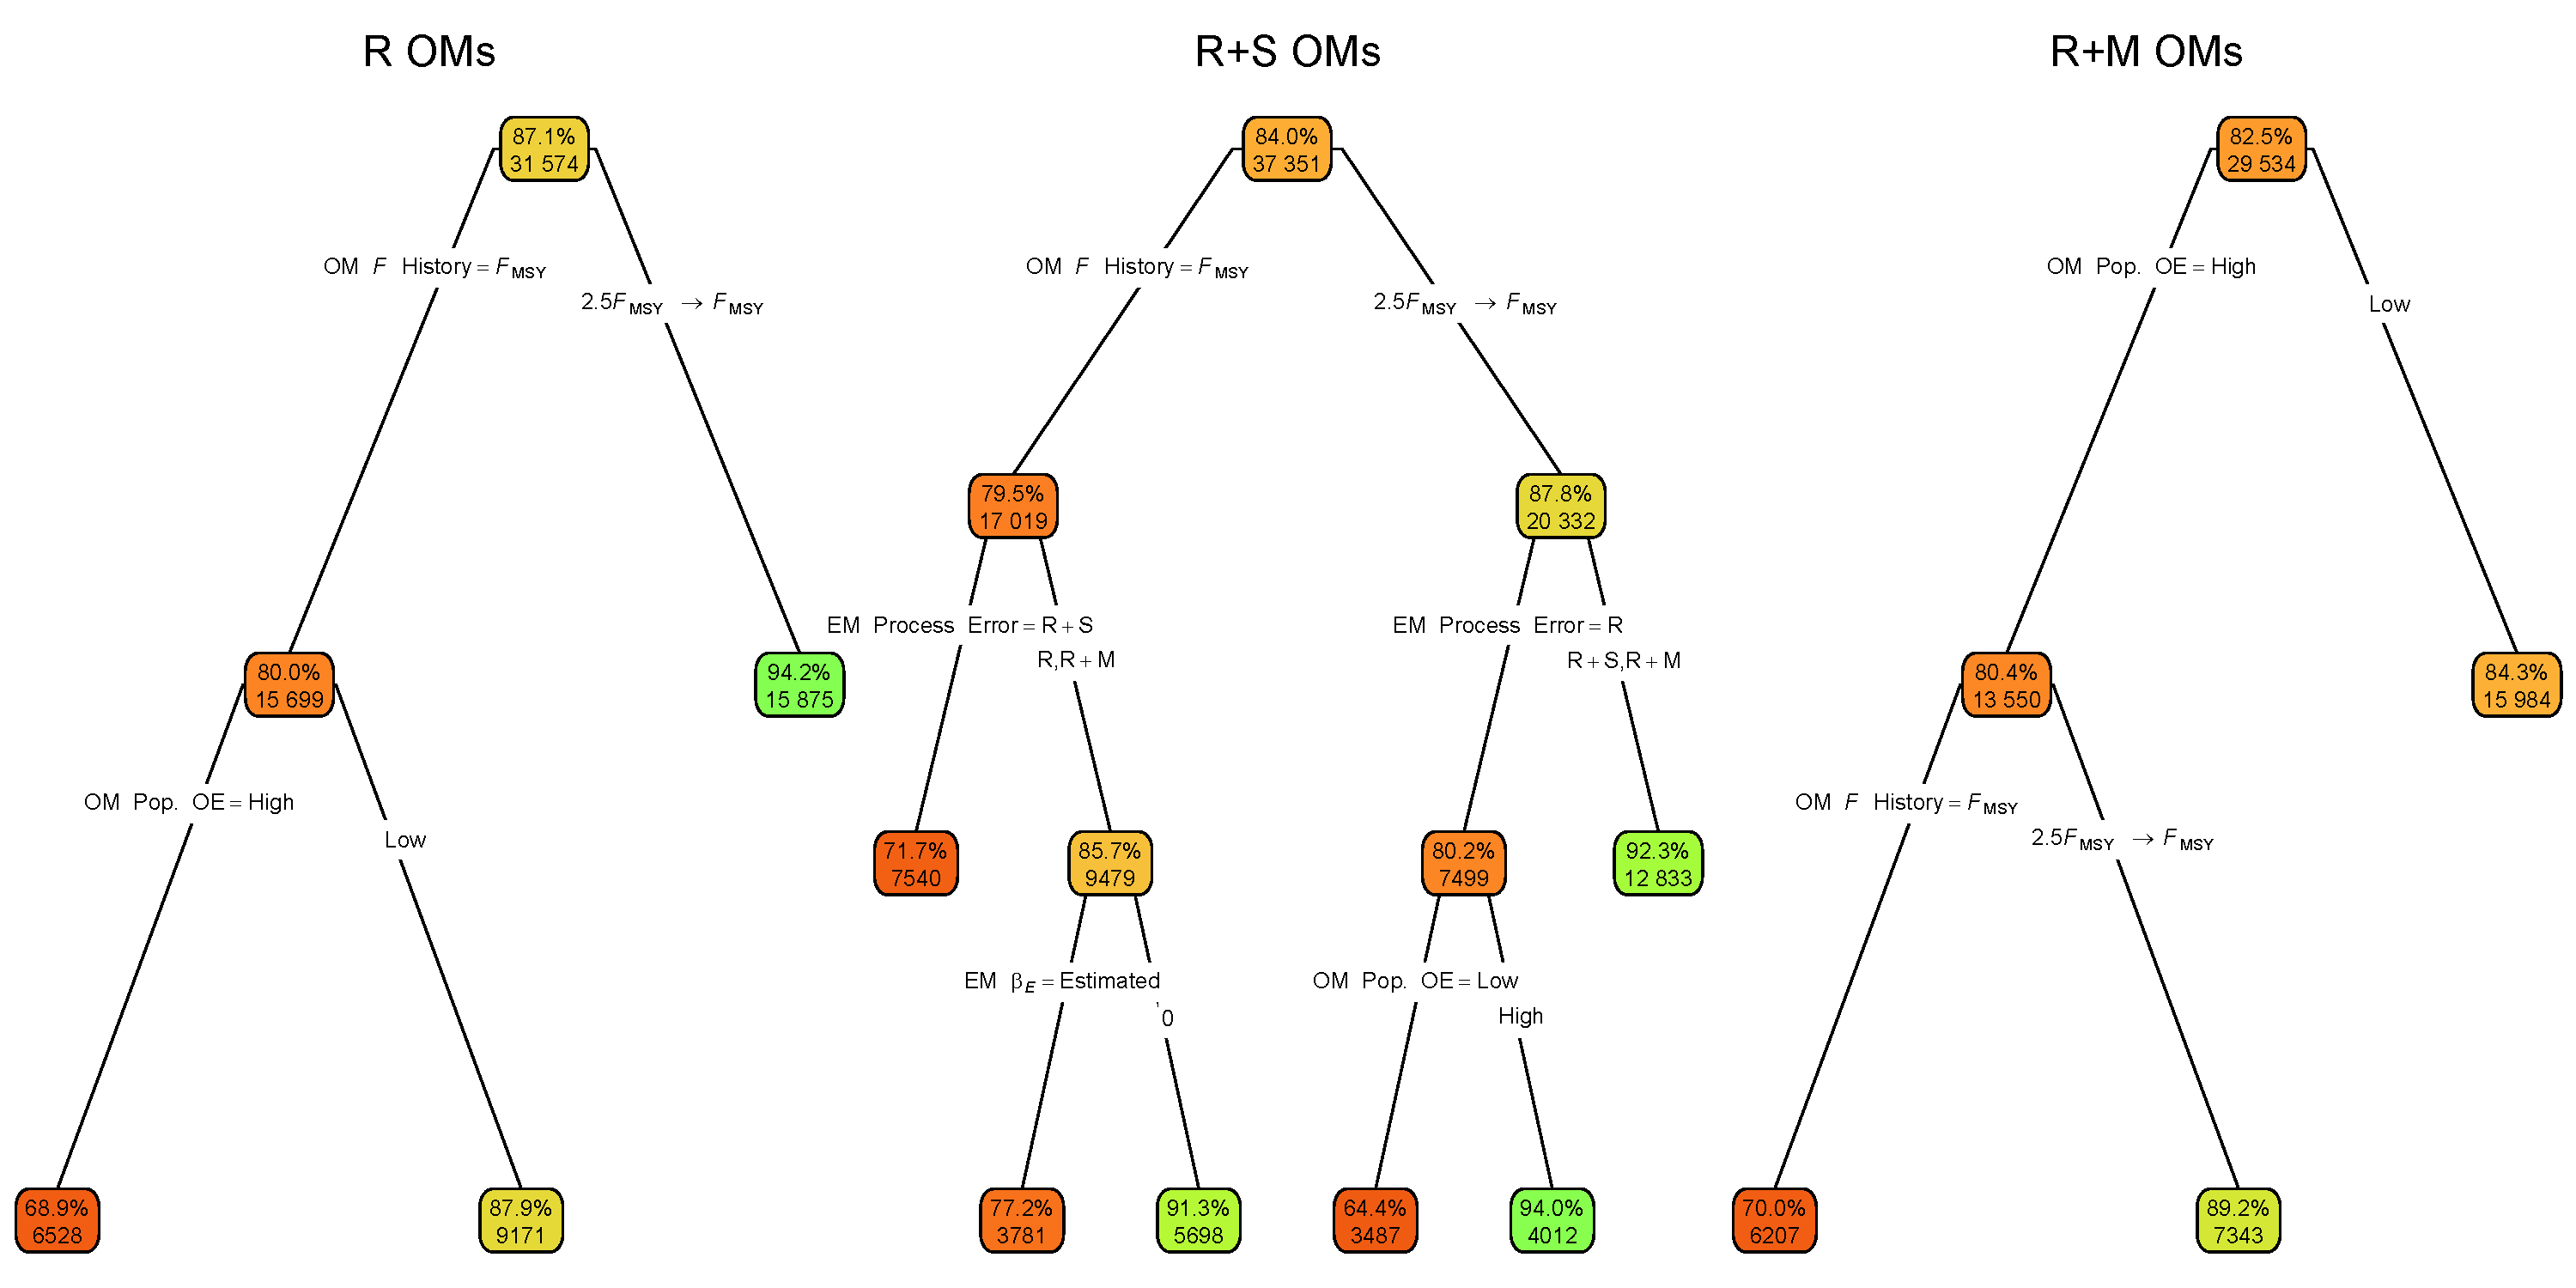
\includegraphics[width = 1.4\textwidth]{median_M_CI_coverage_regtree_plots}
%DIFDELCMD < %%%
\DIFdelendFL \DIFaddbeginFL 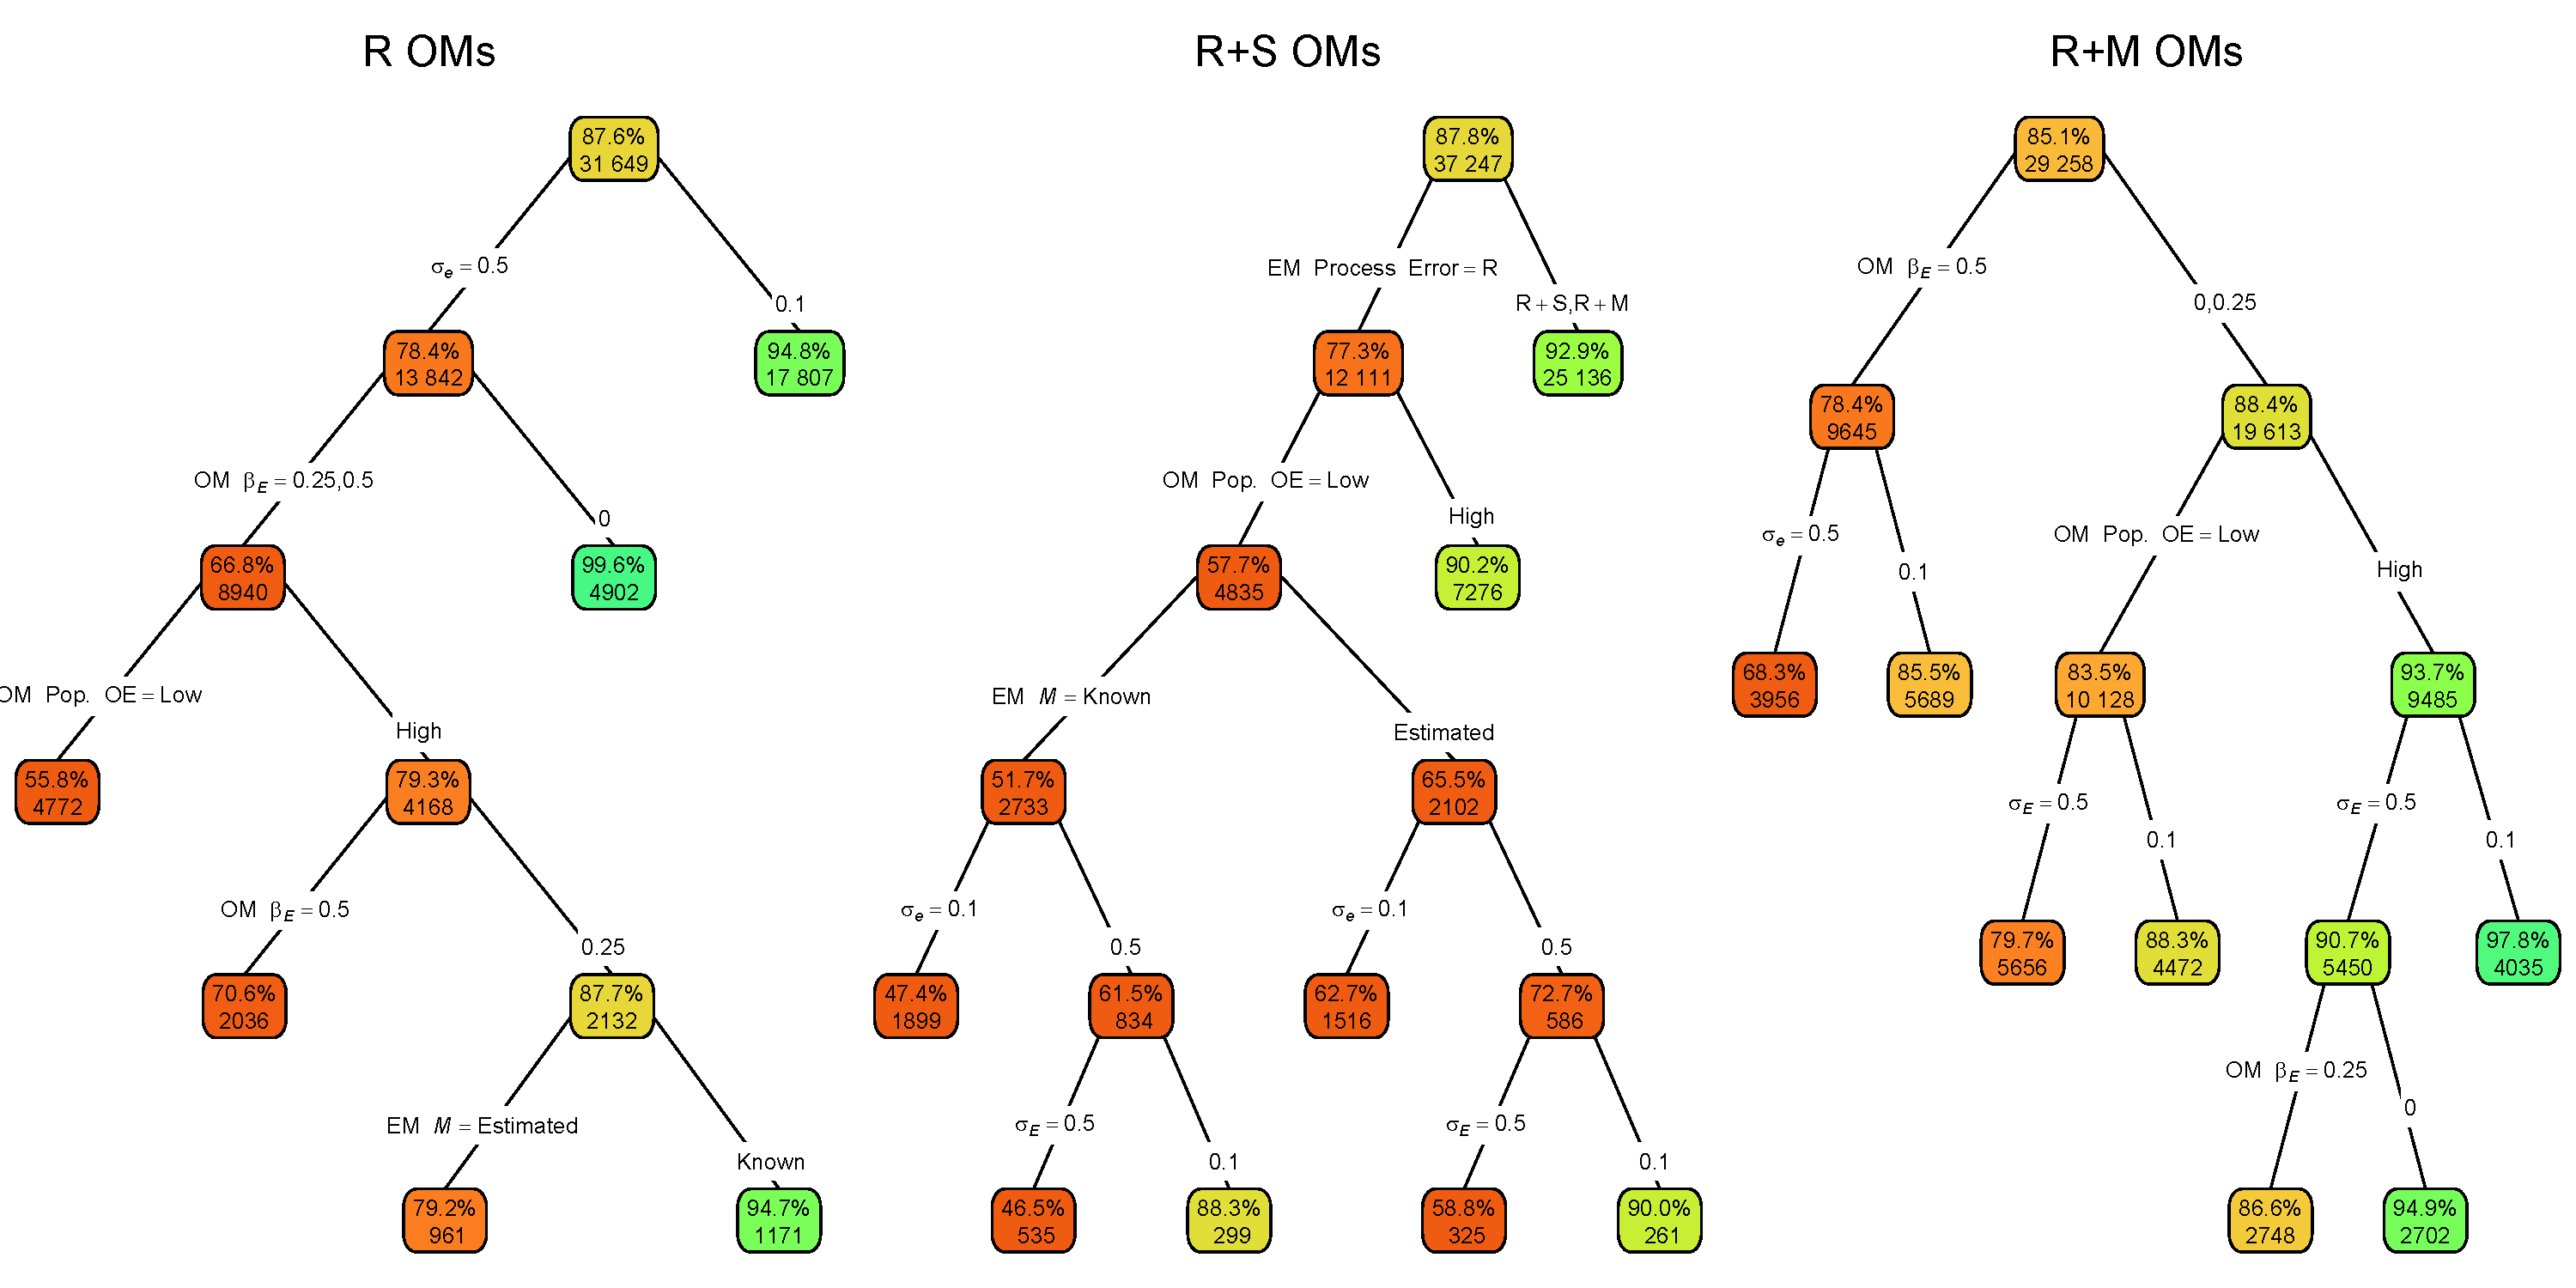
\includegraphics[width = 1.4\textwidth]{ecov_beta_CI_coverage_regtree_plots}
\DIFaddendFL \end{center}
\caption{Classification trees \DIFdelbeginFL \DIFdelFL{indicating primary factors determining }\DIFdelendFL \DIFaddbeginFL \DIFaddFL{for }\DIFaddendFL whether confidence intervals \DIFaddbeginFL \DIFaddFL{(CIs) }\DIFaddendFL for \DIFaddbeginFL \DIFaddFL{the }\DIFaddendFL estimated \DIFdelbeginFL \DIFdelFL{median }\DIFdelendFL \DIFaddbeginFL \DIFaddFL{covariate effects on }\DIFaddendFL $M$ \DIFdelbeginFL \DIFdelFL{parameter }\DIFdelendFL (\DIFdelbeginFL \DIFdelFL{$\beta_M$}\DIFdelendFL \DIFaddbeginFL \DIFaddFL{$\beta_E$}\DIFaddendFL ) \DIFdelbeginFL \DIFdelFL{in estimating models (EMs) fitted to operating models (OMs) with process error on recruitment only (R), recruitment and apparent survival (R+S), or recruitment and natural mortality (R+M) }\DIFdelendFL included the true value. Each node shows the \DIFdelbeginFL \DIFdelFL{median error (top) and number }\DIFdelendFL \DIFaddbeginFL \DIFaddFL{percentage }\DIFaddendFL of \DIFdelbeginFL \DIFdelFL{observations (bottom) }\DIFdelendFL \DIFaddbeginFL \DIFaddFL{CIs that include the true value }\DIFaddendFL for the corresponding subset. \DIFdelbeginFL \DIFdelFL{Lower }\DIFdelendFL \DIFaddbeginFL \DIFaddFL{Higher }\DIFaddendFL or \DIFdelbeginFL \DIFdelFL{higher median absolute errors of the process error assumption }\DIFdelendFL \DIFaddbeginFL \DIFaddFL{lower percentages }\DIFaddendFL are indicated by more green or red polygons, respectively. See \DIFaddbeginFL \DIFaddFL{Figure \ref{conv_class} caption and }\DIFaddendFL Table \ref{factor_table} for \DIFdelbeginFL \DIFdelFL{description of OM and EM factors defining nodes and branches}\DIFdelendFL \DIFaddbeginFL \DIFaddFL{further details}\DIFaddendFL .}\DIFdelbeginFL %DIFDELCMD < \label{med_M_CI_coverage_regtree}
%DIFDELCMD < %%%
\DIFdelendFL \DIFaddbeginFL \label{ecov_effect_CI_coverage_regtree}
\DIFaddendFL \end{figure}
\end{landscape}

\begin{landscape}
\begin{figure}
\begin{center}
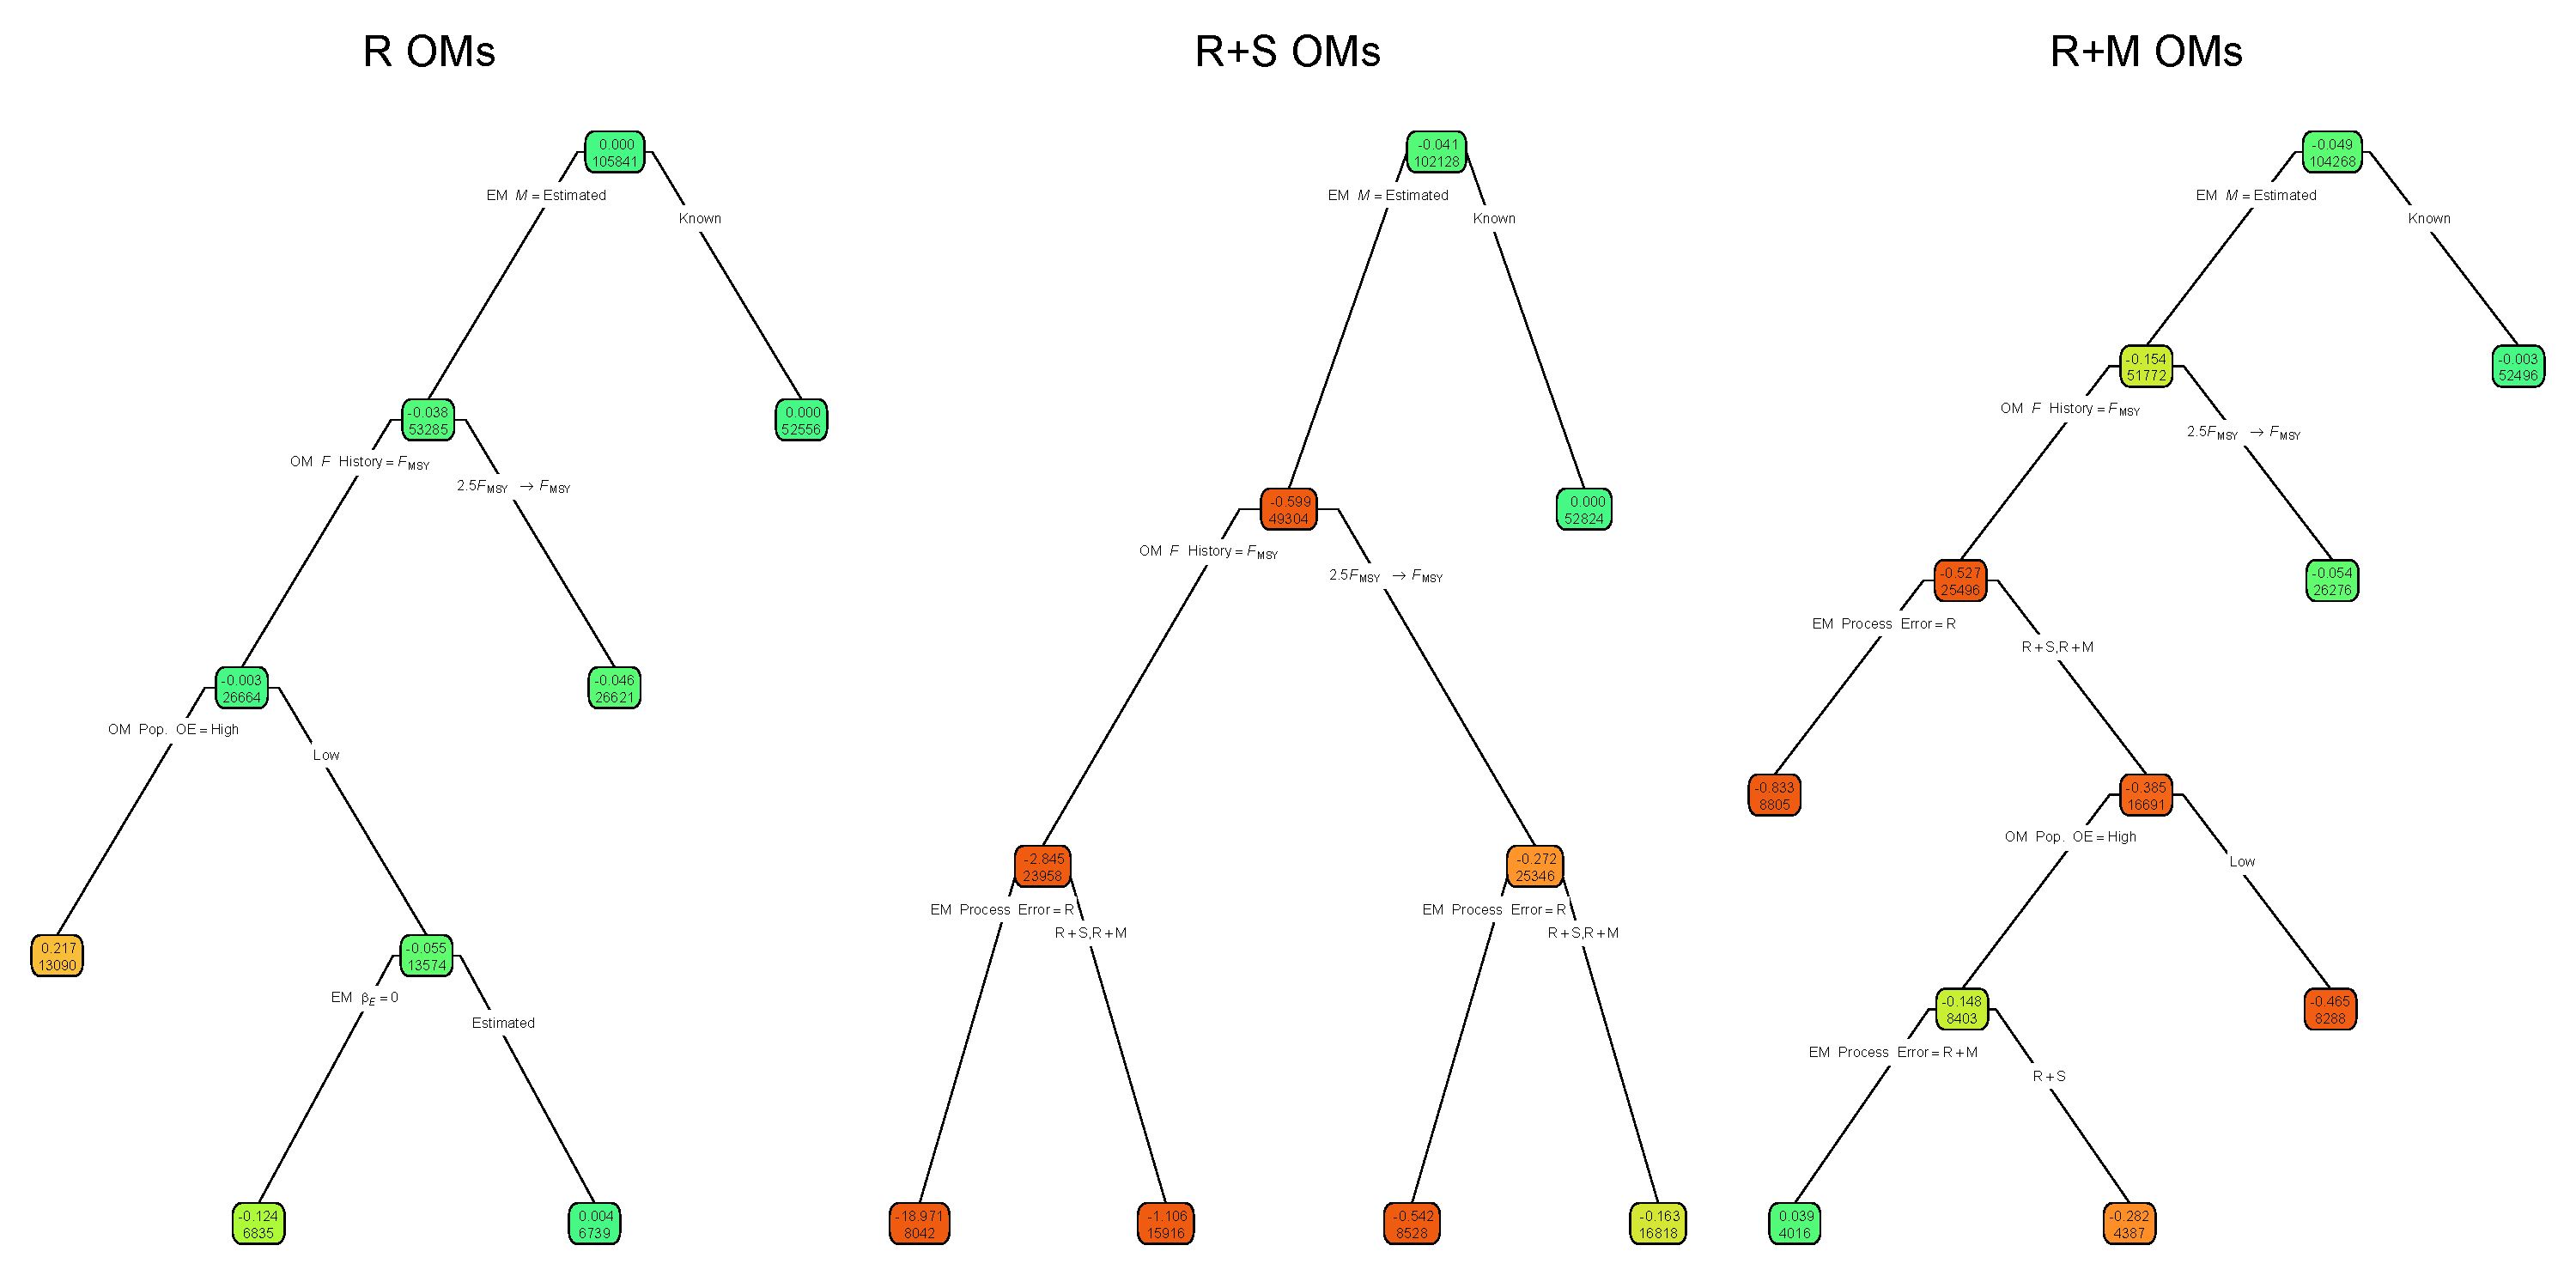
\includegraphics[width = 1.4\textwidth]{term_M_bias_regtree_plots}
\end{center}
\caption{Regression trees \DIFdelbeginFL \DIFdelFL{indicating primary factors determining reductions in sums of squares of errors in }\DIFdelendFL \DIFaddbeginFL \DIFaddFL{for }\DIFaddendFL estimation \DIFaddbeginFL \DIFaddFL{error of terminal year $M$ as }\DIFaddendFL measured by Eq. \ref{relerror_trans_response}\DIFdelbeginFL \DIFdelFL{for the terminal year $M$ in estimating models (EMs) fitted to operating models (OMs) with process error on recruitment only (R), recruitment and apparent survival (R+S), or recruitment and natural mortality (R+M)}\DIFdelendFL . Each node shows the median error \DIFdelbeginFL \DIFdelFL{(top) and number of observations (bottom) }\DIFdelendFL for the corresponding subset. Lower or higher \DIFdelbeginFL \DIFdelFL{median }\DIFdelendFL absolute \DIFaddbeginFL \DIFaddFL{median }\DIFaddendFL errors \DIFdelbeginFL \DIFdelFL{of the process error assumption }\DIFdelendFL are indicated by more green or red polygons, respectively. See \DIFaddbeginFL \DIFaddFL{Figure \ref{conv_class} caption and }\DIFaddendFL Table \ref{factor_table} for \DIFdelbeginFL \DIFdelFL{description of OM and EM factors defining nodes and branches}\DIFdelendFL \DIFaddbeginFL \DIFaddFL{further details}\DIFaddendFL .}\label{term_M_bias_regtree}
\end{figure}
\end{landscape}

\begin{landscape}
\begin{figure}
\begin{center}
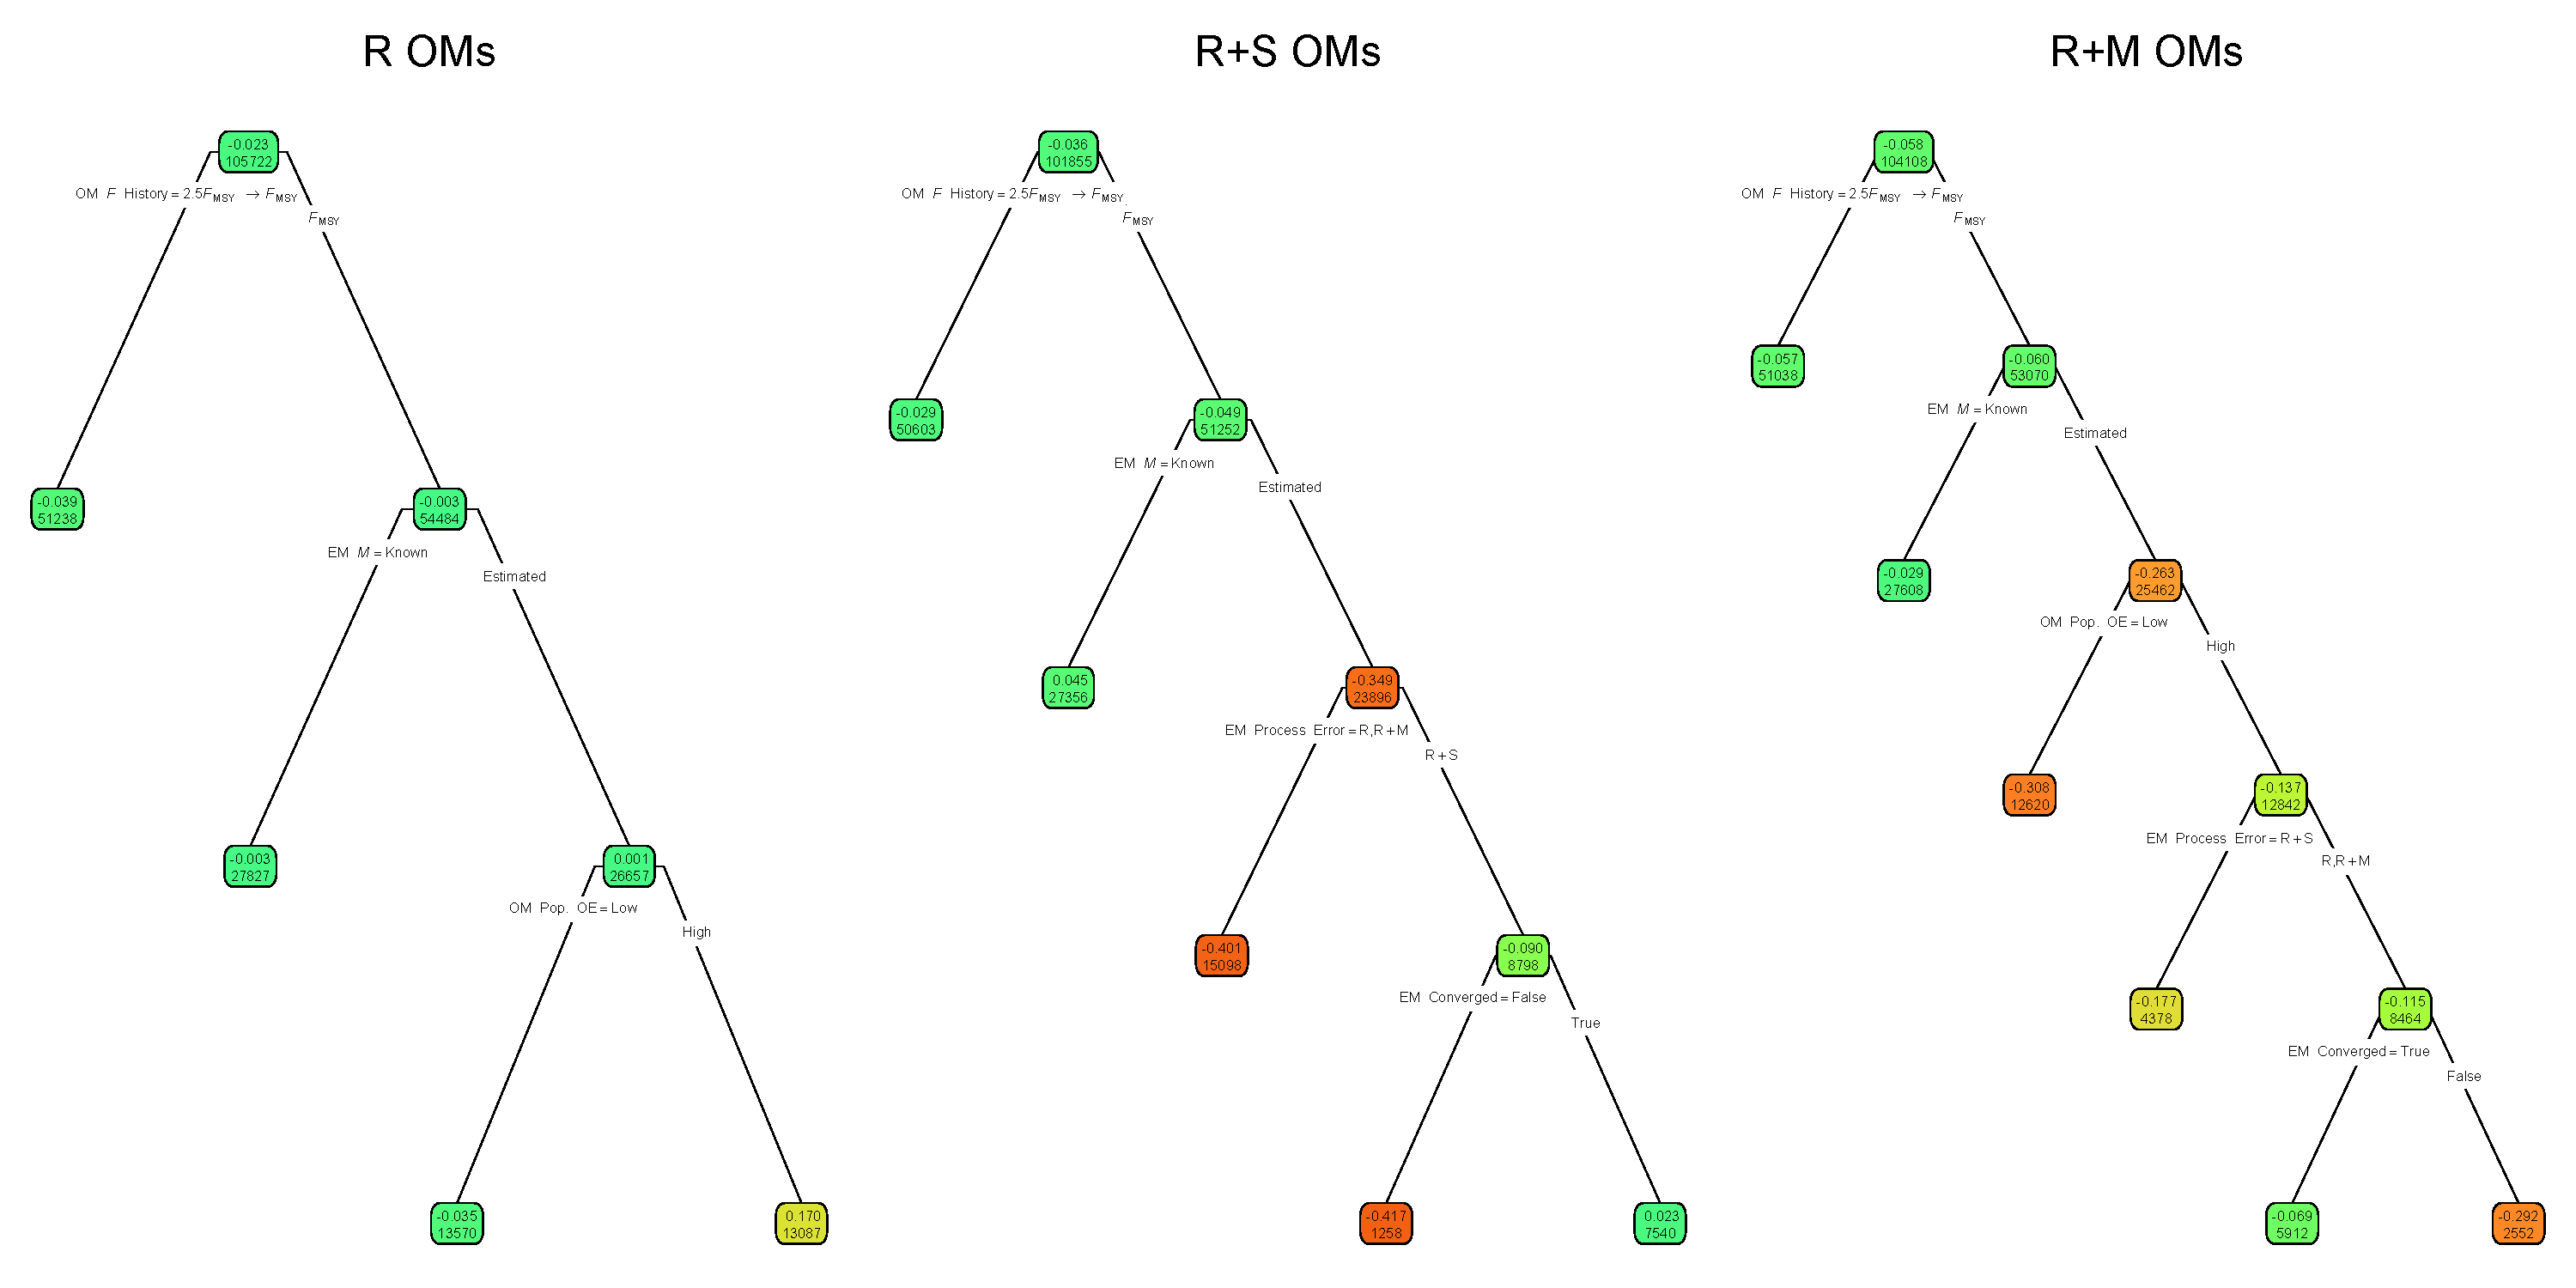
\includegraphics[width = 1.4\textwidth]{term_SSB_bias_regtree_plots}
\end{center}
\caption{Regression trees \DIFdelbeginFL \DIFdelFL{indicating primary factors determining reductions in sums of squares of errors in }\DIFdelendFL \DIFaddbeginFL \DIFaddFL{for }\DIFaddendFL estimation \DIFaddbeginFL \DIFaddFL{error of terminal year SSB as }\DIFaddendFL measured by Eq. \ref{relerror_trans_response}\DIFdelbeginFL \DIFdelFL{for the terminal year SSB in estimating models (EMs) fitted to operating models (OMs) with process error on recruitment only (R), recruitment and apparent survival (R+S), or recruitment and natural mortality (R+M)}\DIFdelendFL . Each node shows the median error \DIFdelbeginFL \DIFdelFL{(top) and number of observations (bottom) }\DIFdelendFL for the corresponding subset. Lower or higher \DIFdelbeginFL \DIFdelFL{median }\DIFdelendFL absolute \DIFaddbeginFL \DIFaddFL{median }\DIFaddendFL errors \DIFdelbeginFL \DIFdelFL{of the process error assumption }\DIFdelendFL are indicated by more green or red polygons, respectively. See \DIFaddbeginFL \DIFaddFL{Figure \ref{conv_class} caption and }\DIFaddendFL Table \ref{factor_table} for \DIFdelbeginFL \DIFdelFL{description of OM and EM factors defining nodes and branches}\DIFdelendFL \DIFaddbeginFL \DIFaddFL{further details}\DIFaddendFL .}\label{term_SSB_bias_regtree}
\end{figure}
\end{landscape}

\pagebreak

\DIFaddbegin \setcounter{figure}{0}
\renewcommand\thefigure{S\arabic{figure}}

\setcounter{table}{0}
\renewcommand\thetable{S\arabic{table}}

\begin{landscape}
\end{landscape}

\section*{\DIFadd{Supplemental Materials}}\label{supplemental-materials}
\addcontentsline{toc}{section}{\DIFadd{Supplemental Materials}}

\subsection*{\DIFadd{Referenced Figures and Tables}}\label{referenced-figures-and-tables}
\addcontentsline{toc}{subsection}{\DIFadd{Referenced Figures and Tables}}

\begin{landscape}
\begin{figure}
\begin{center}
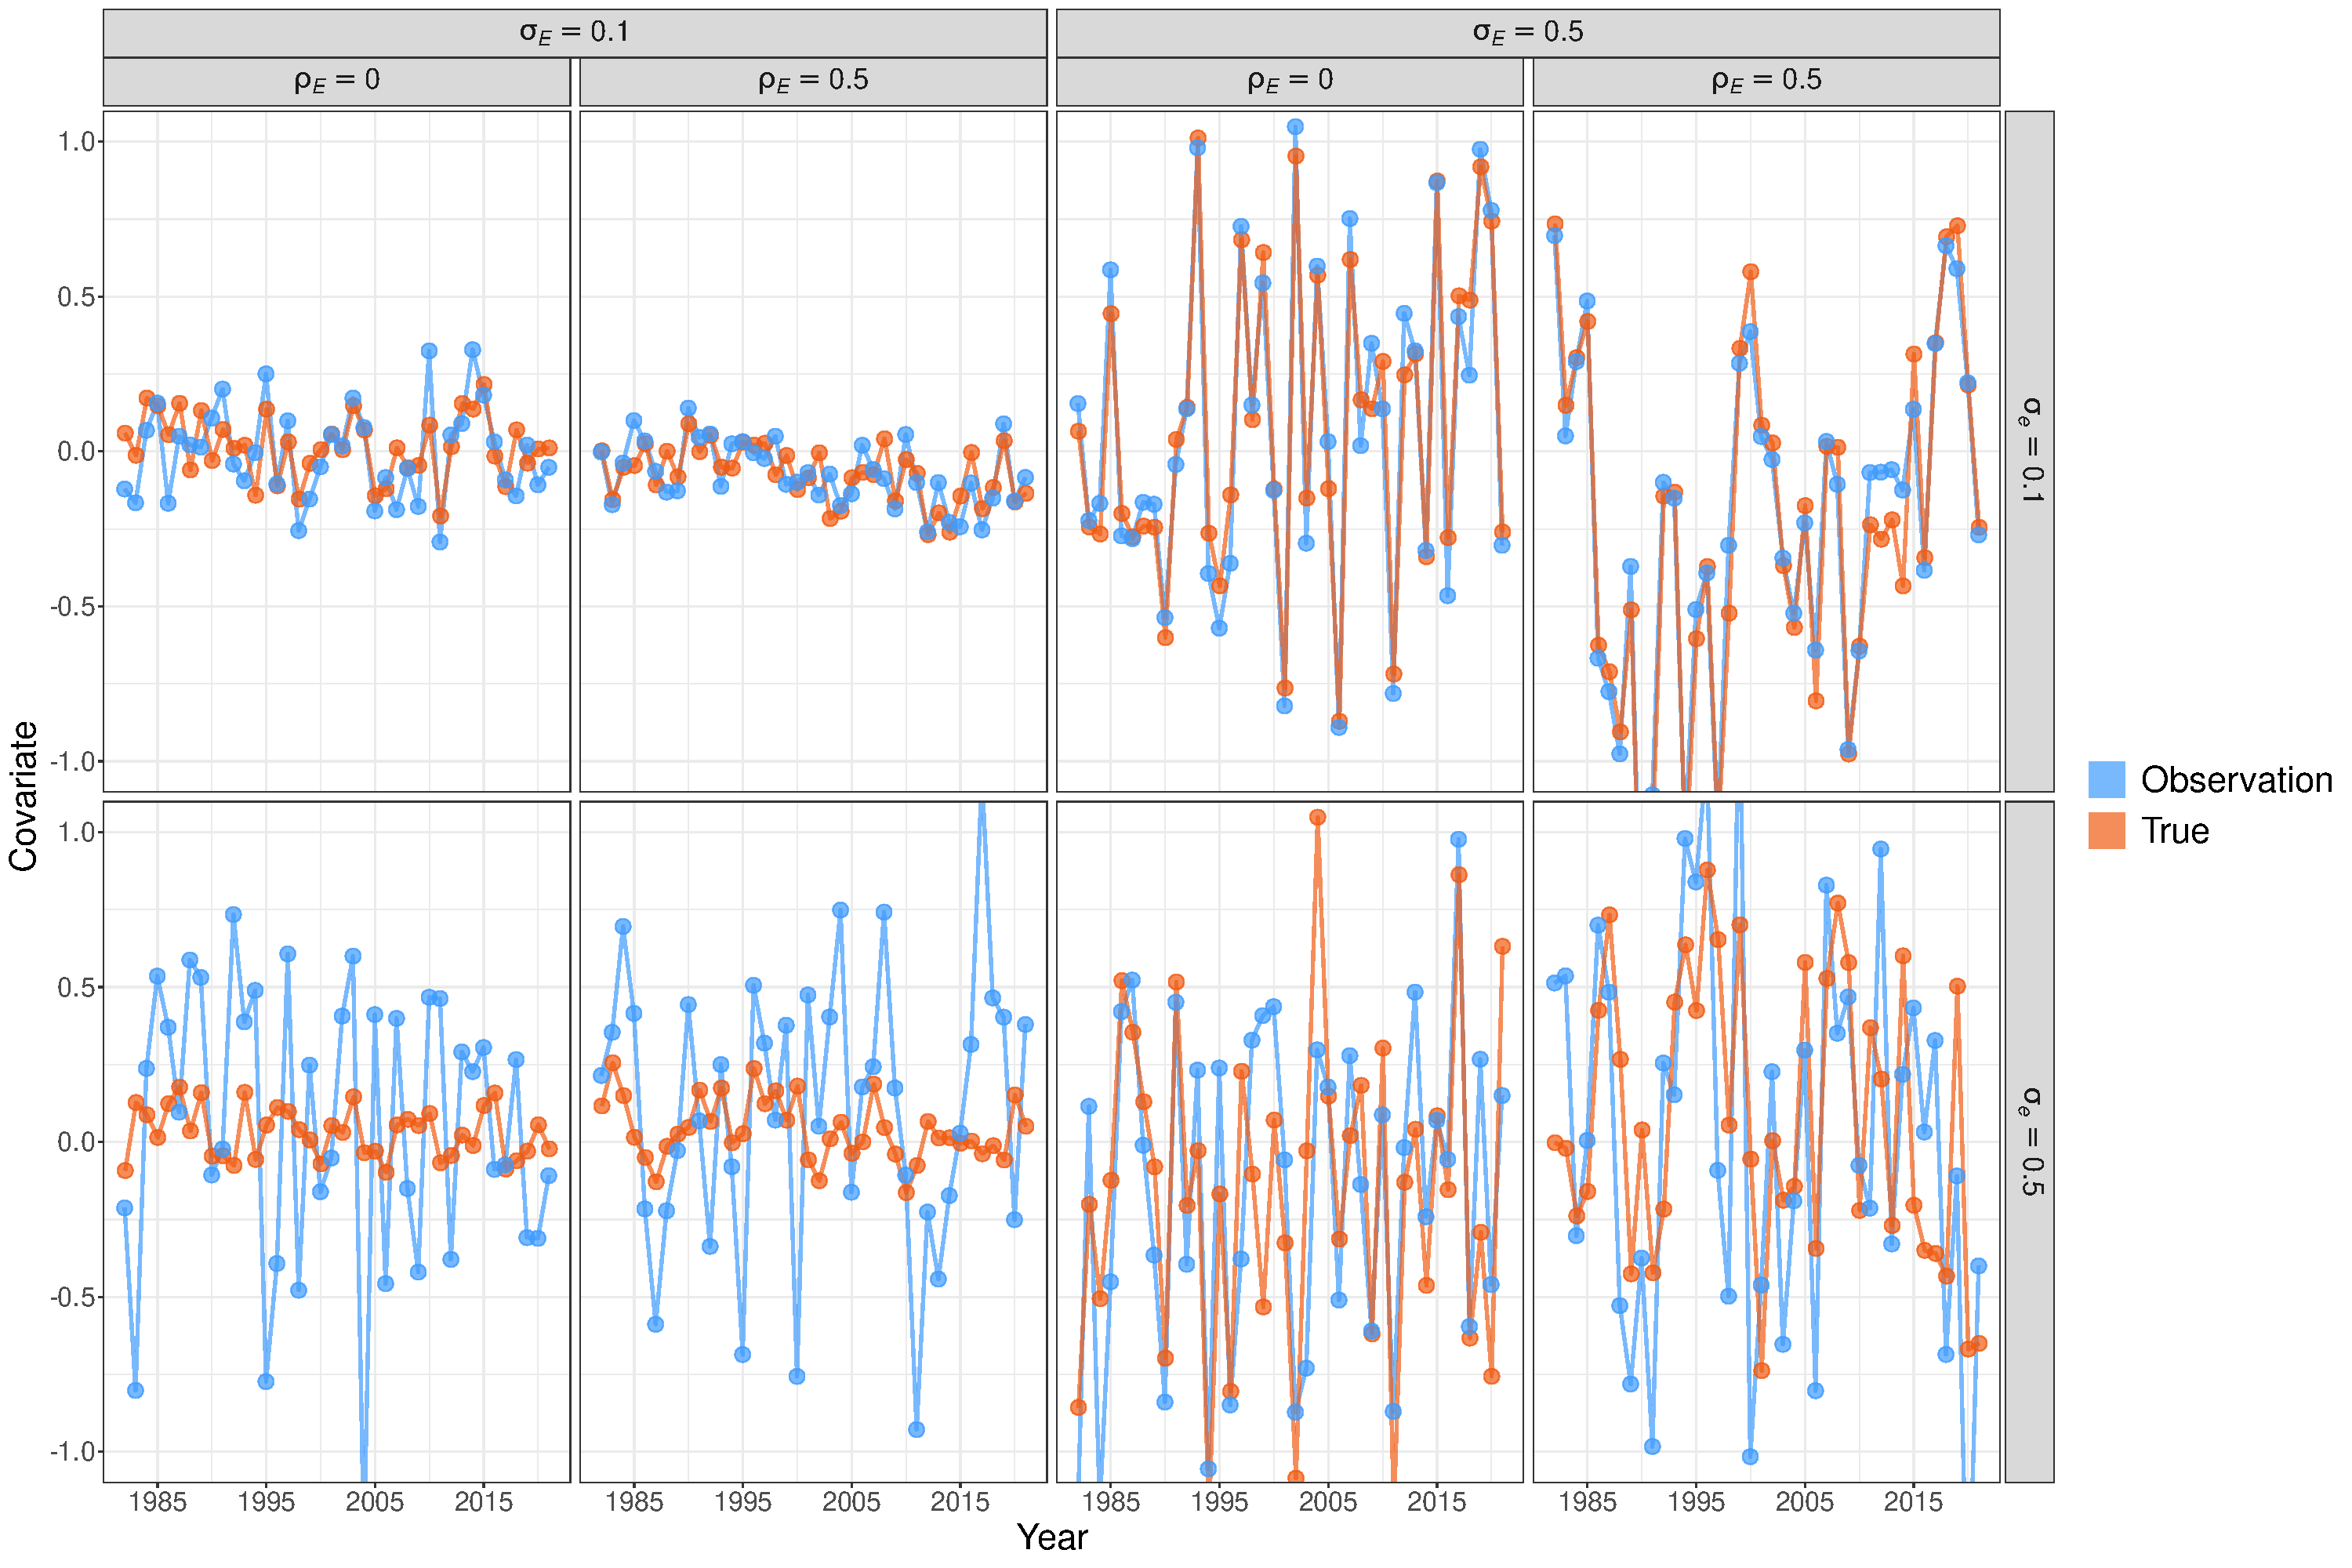
\includegraphics[height = \textheight]{Ecov_true_obs_example}
\end{center}
\caption{\DIFaddFL{Example simulations of environmental covariate latent processes and observations with different levels of observation error, and different assumptions about variability of the latent process.}}\label{om_ecov_example}
\end{figure}
\end{landscape}

\begin{figure}
\begin{center}
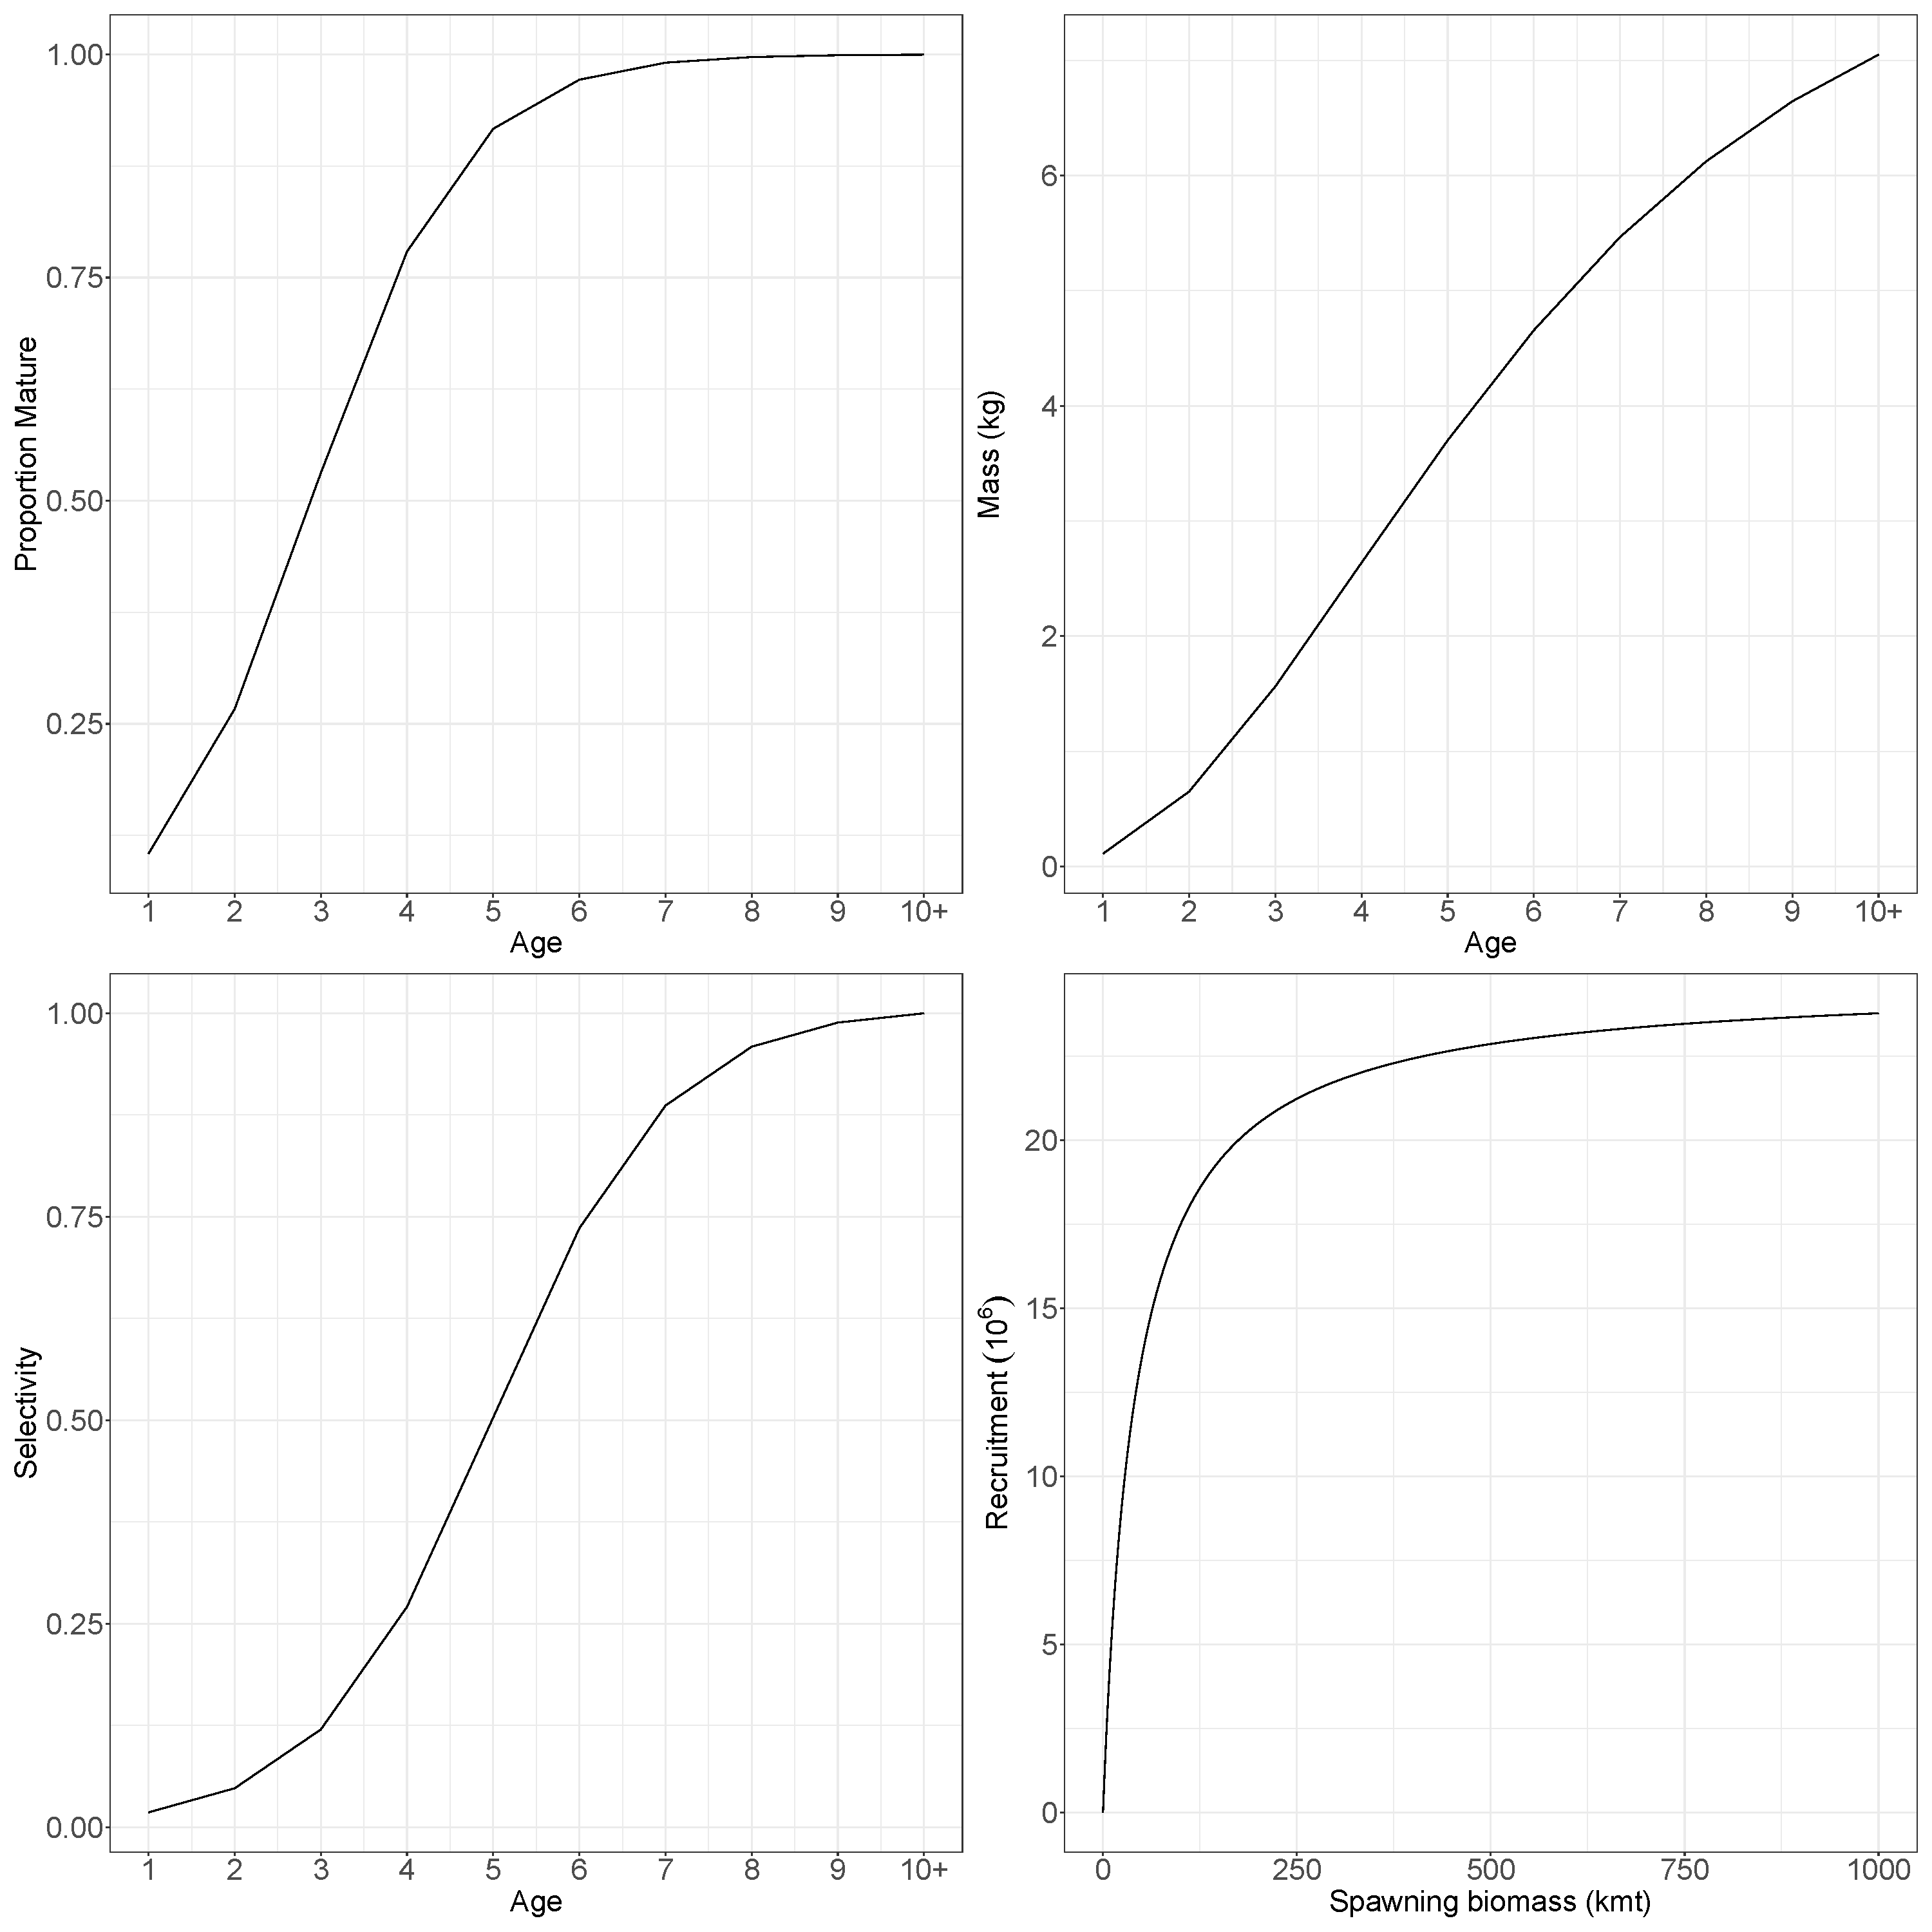
\includegraphics[width = \textwidth]{om_input_plots_figure}
\end{center}
\caption{\DIFaddFL{The proportion mature at age, weight at age, fleet and index selectivity at age, and Beverton-Holt stock-recruit relationship assumed for the population in all operating models. For operating models with random effects on fleet selectivity, this represents the selectivity at the mean of the random effects.}}\label{om_inputs_fig}
\end{figure}

\begin{landscape}
\begin{figure}
\begin{center}
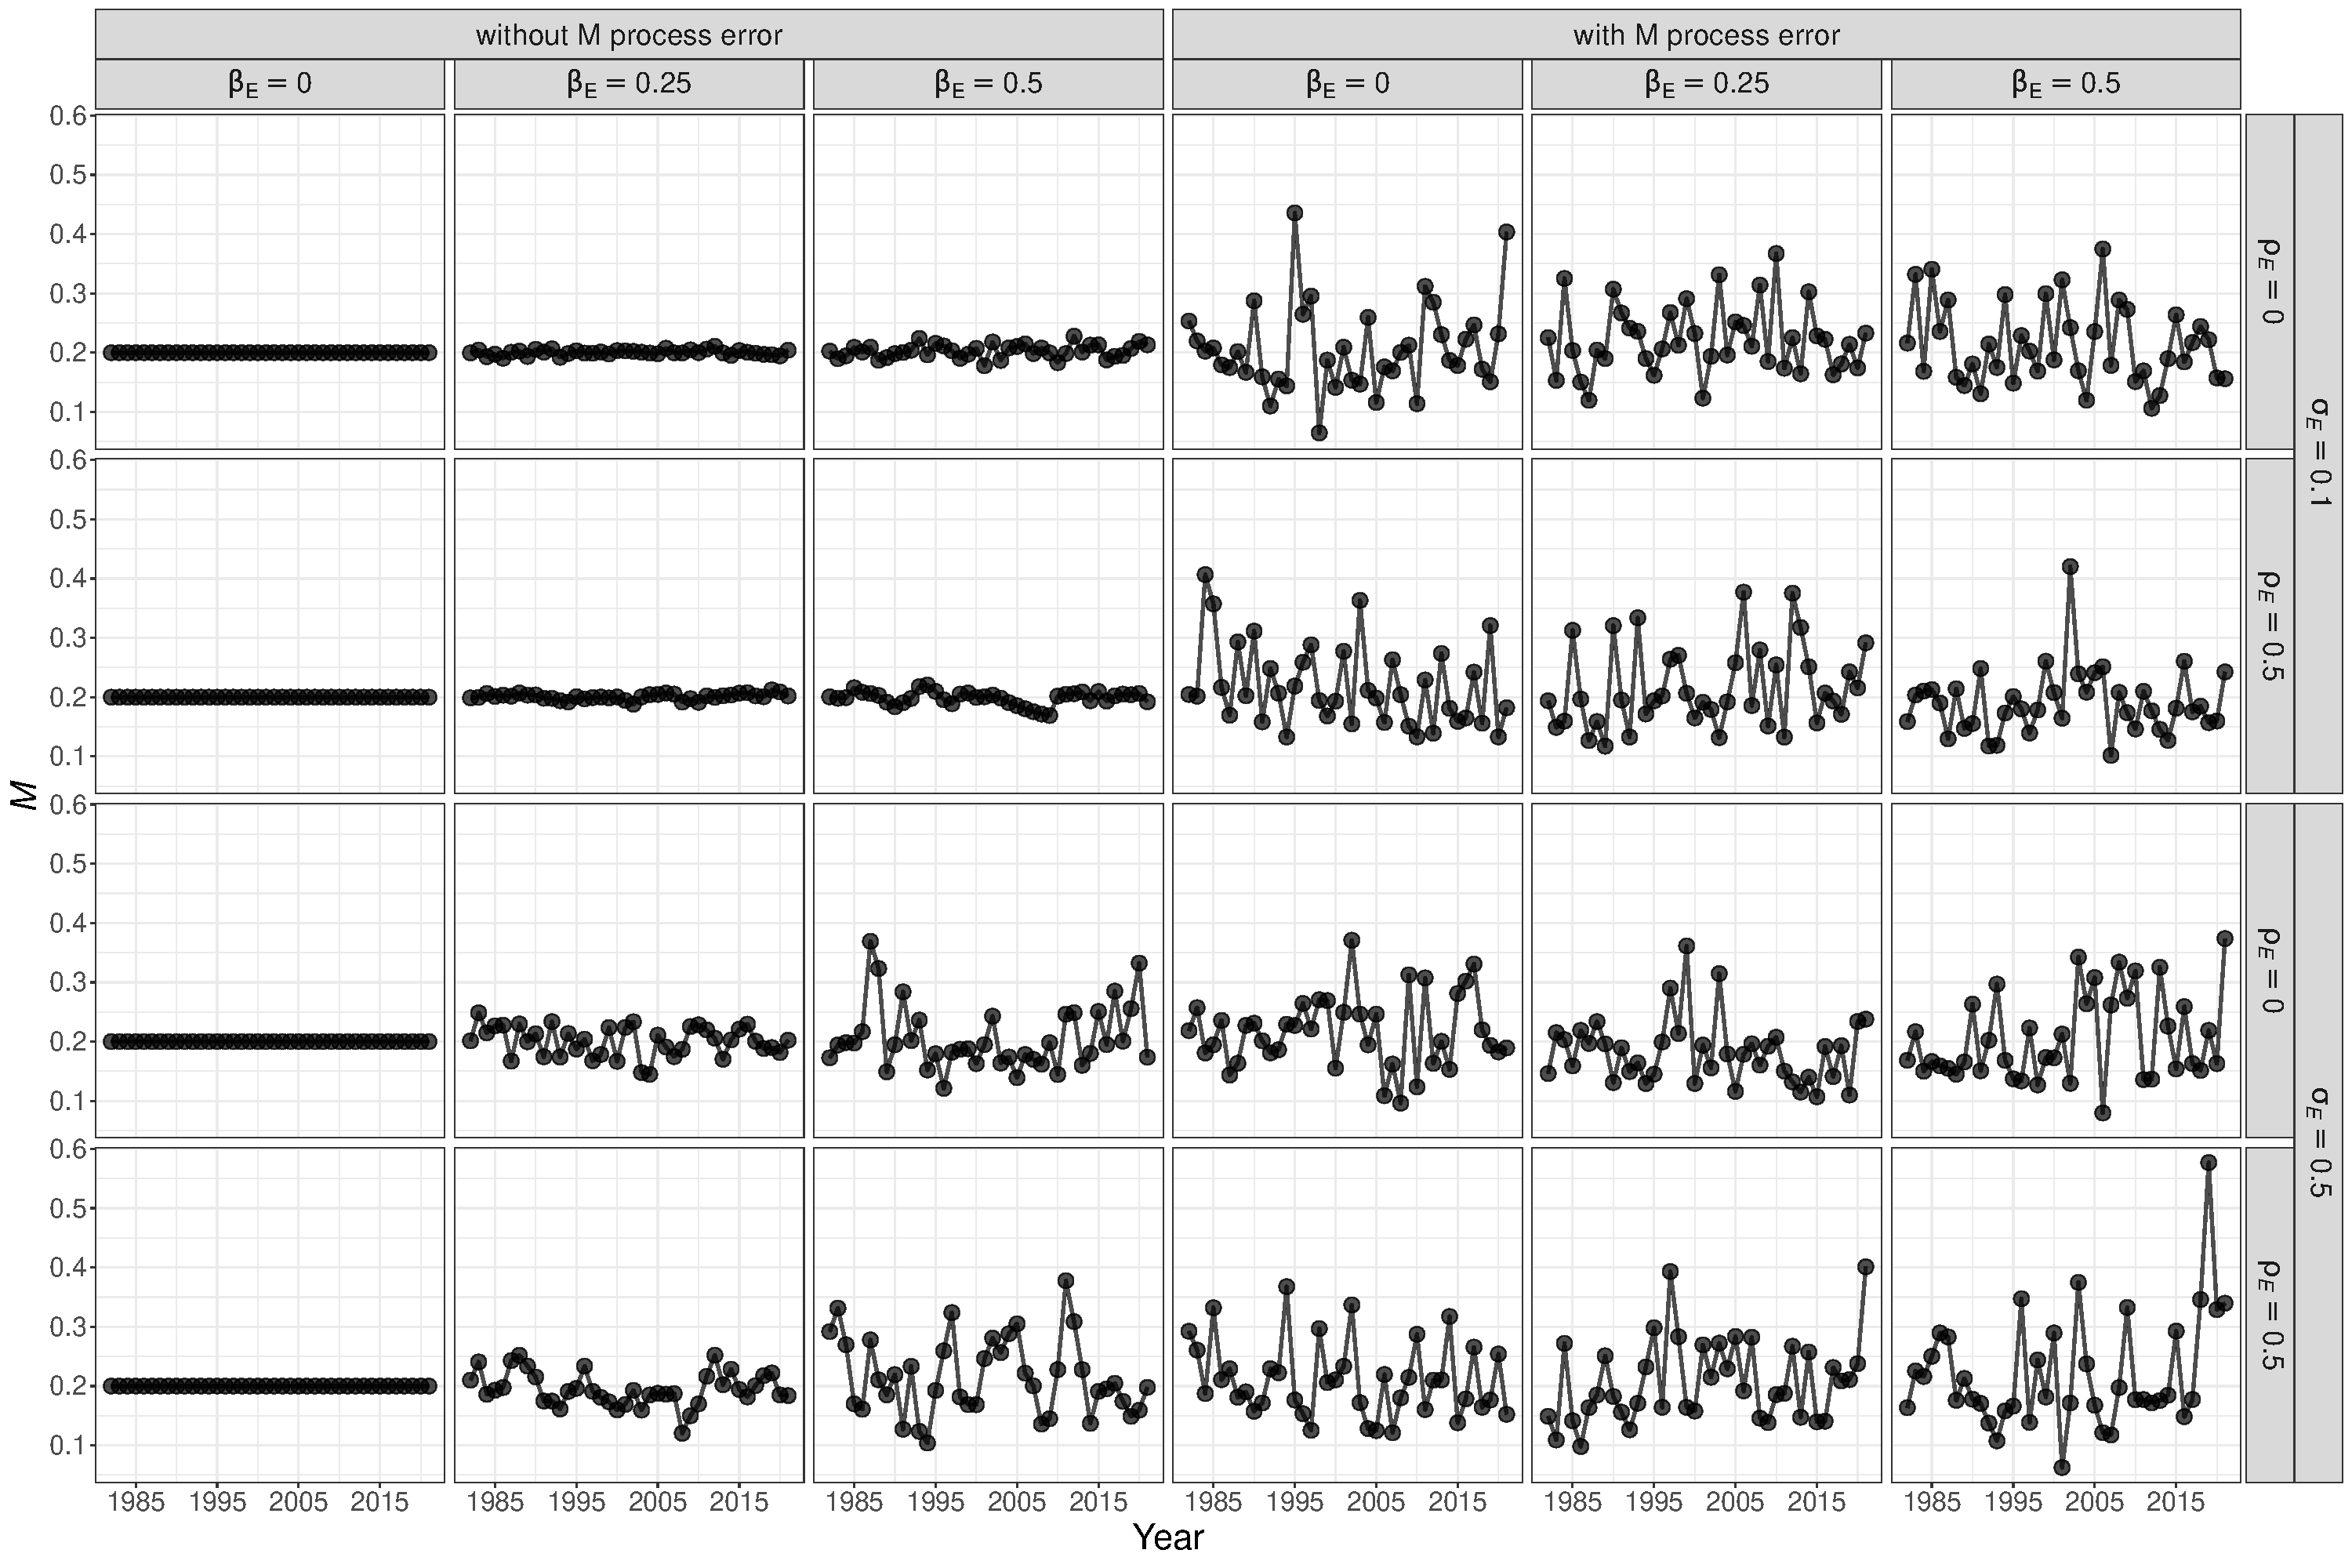
\includegraphics[height = \textheight]{M_example}
\end{center}
\caption{\DIFaddFL{Example simulations of annual $M$ that may be a function of a temporally varying environmental covariate and autoregressive random effects. The marginal standard devation of random effects is $\sigma_M = 0.3$.}}\label{M_example}
\end{figure}
\end{landscape}

\begin{landscape}
\begin{figure}
\begin{center}
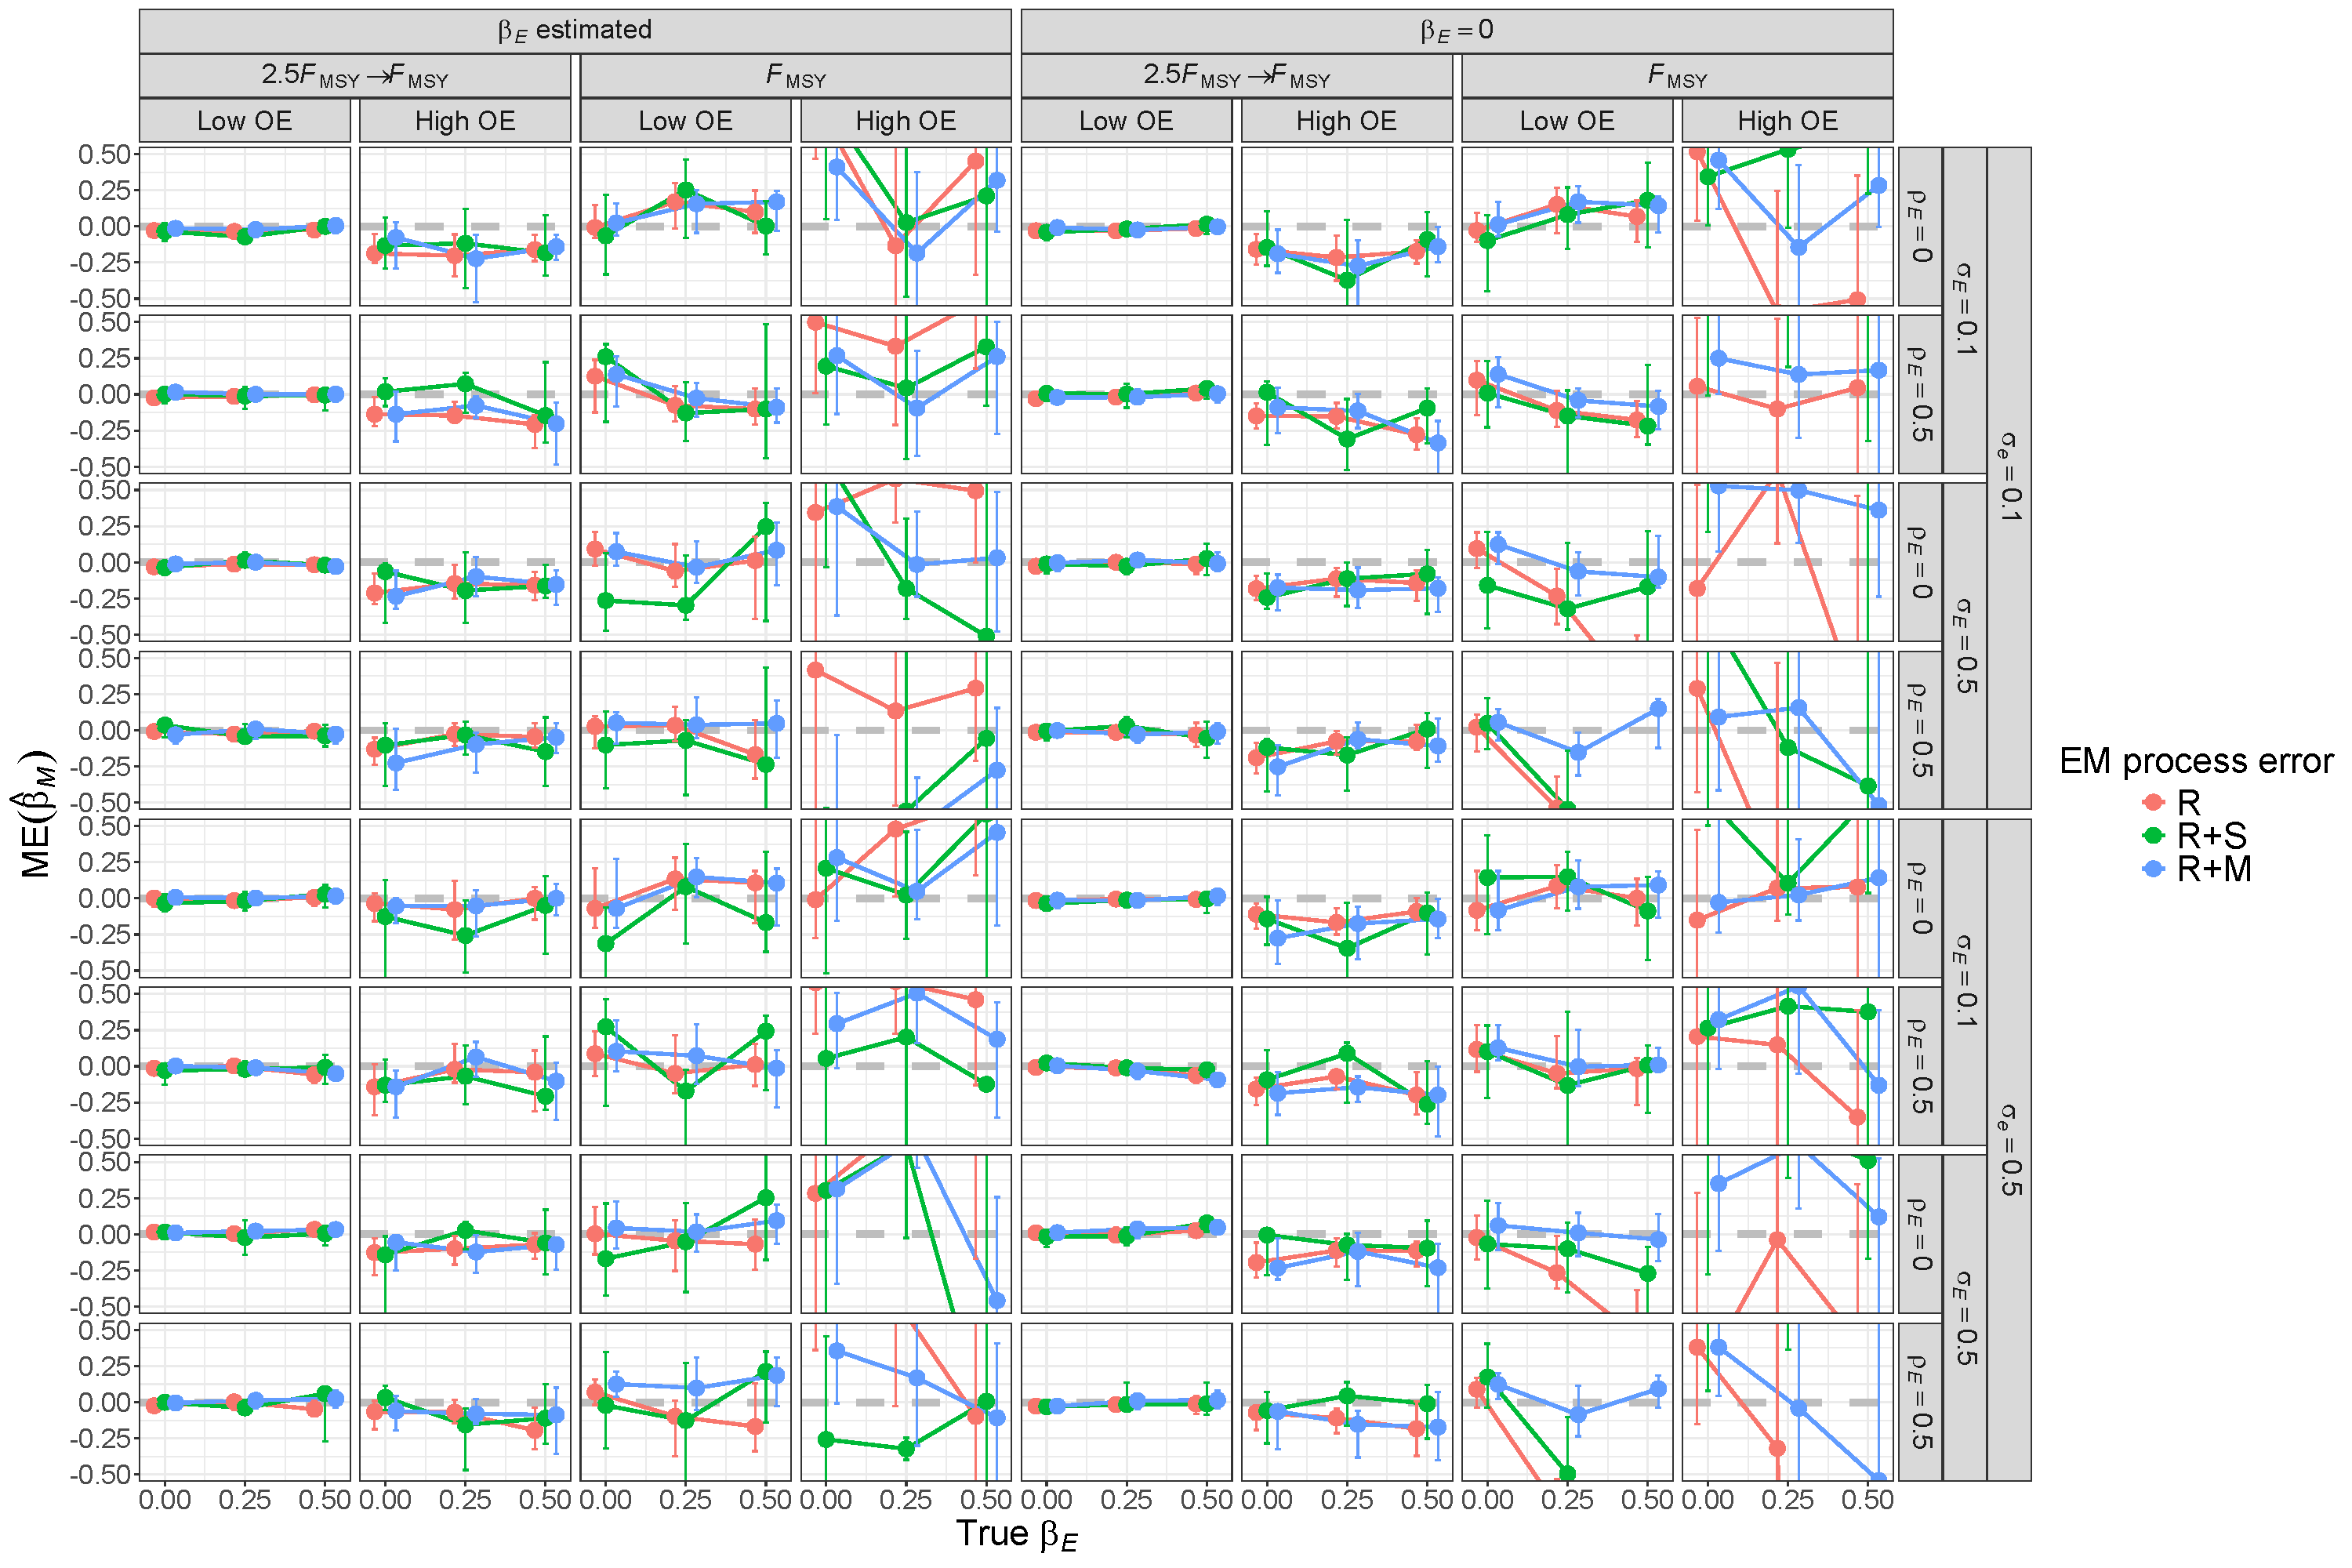
\includegraphics[height = \textheight]{beta_M_bias_Rom}
\end{center}
\caption{\DIFaddFL{For R operating models, median error (ME) of estimates of $\beta_M$ from fitting estimating models with alternative process error assumptions and treatment of covariate effect ($\beta_E = 0$ or estimated). Vertical lines represent 95\% confidence intervals.}}\label{beta_M_bias_Rom}
\end{figure}
\end{landscape}

\begin{landscape}
\begin{figure}
\begin{center}
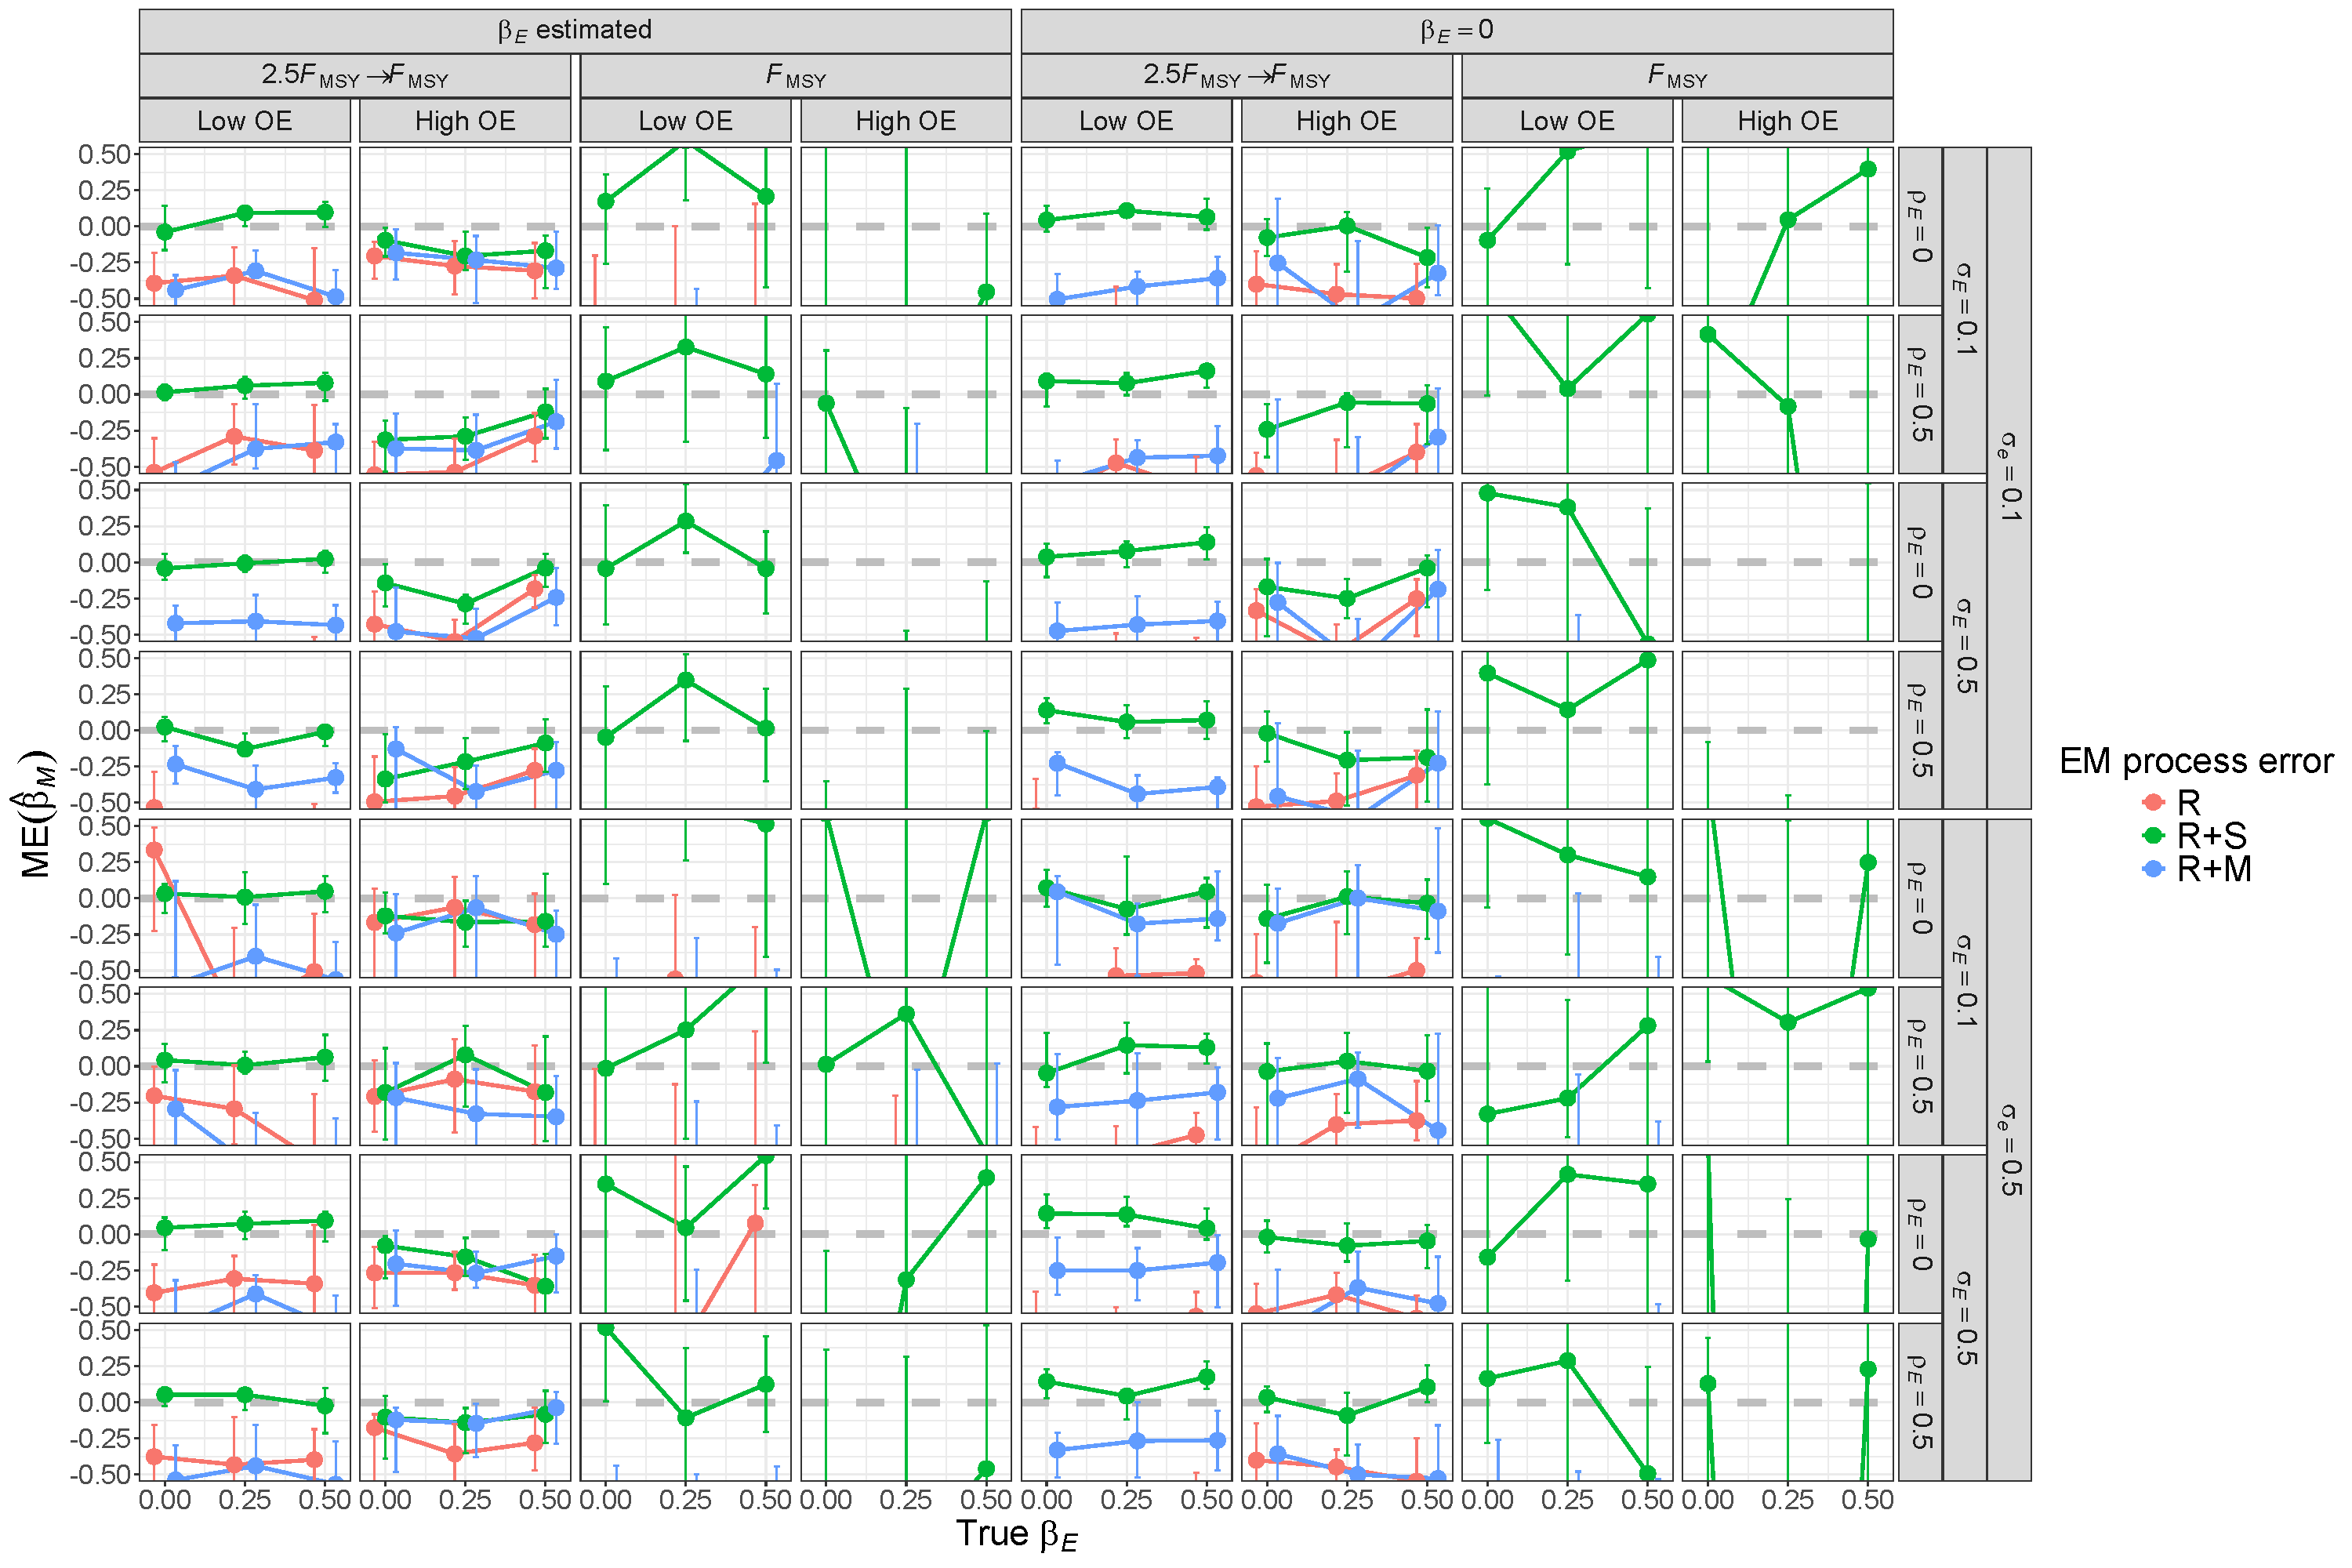
\includegraphics[height = \textheight]{beta_M_bias_RSom}
\end{center}
\caption{\DIFaddFL{For R+S operating models, median error (ME) of estimates of $\beta_M$ from fitting estimating models with alternative process error assumptions and treatment of covariate effect ($\beta_E = 0$ or estimated). Vertical lines represent 95\% confidence intervals.}}\label{beta_M_bias_RSom}
\end{figure}
\end{landscape}

\begin{landscape}
\begin{figure}
\begin{center}
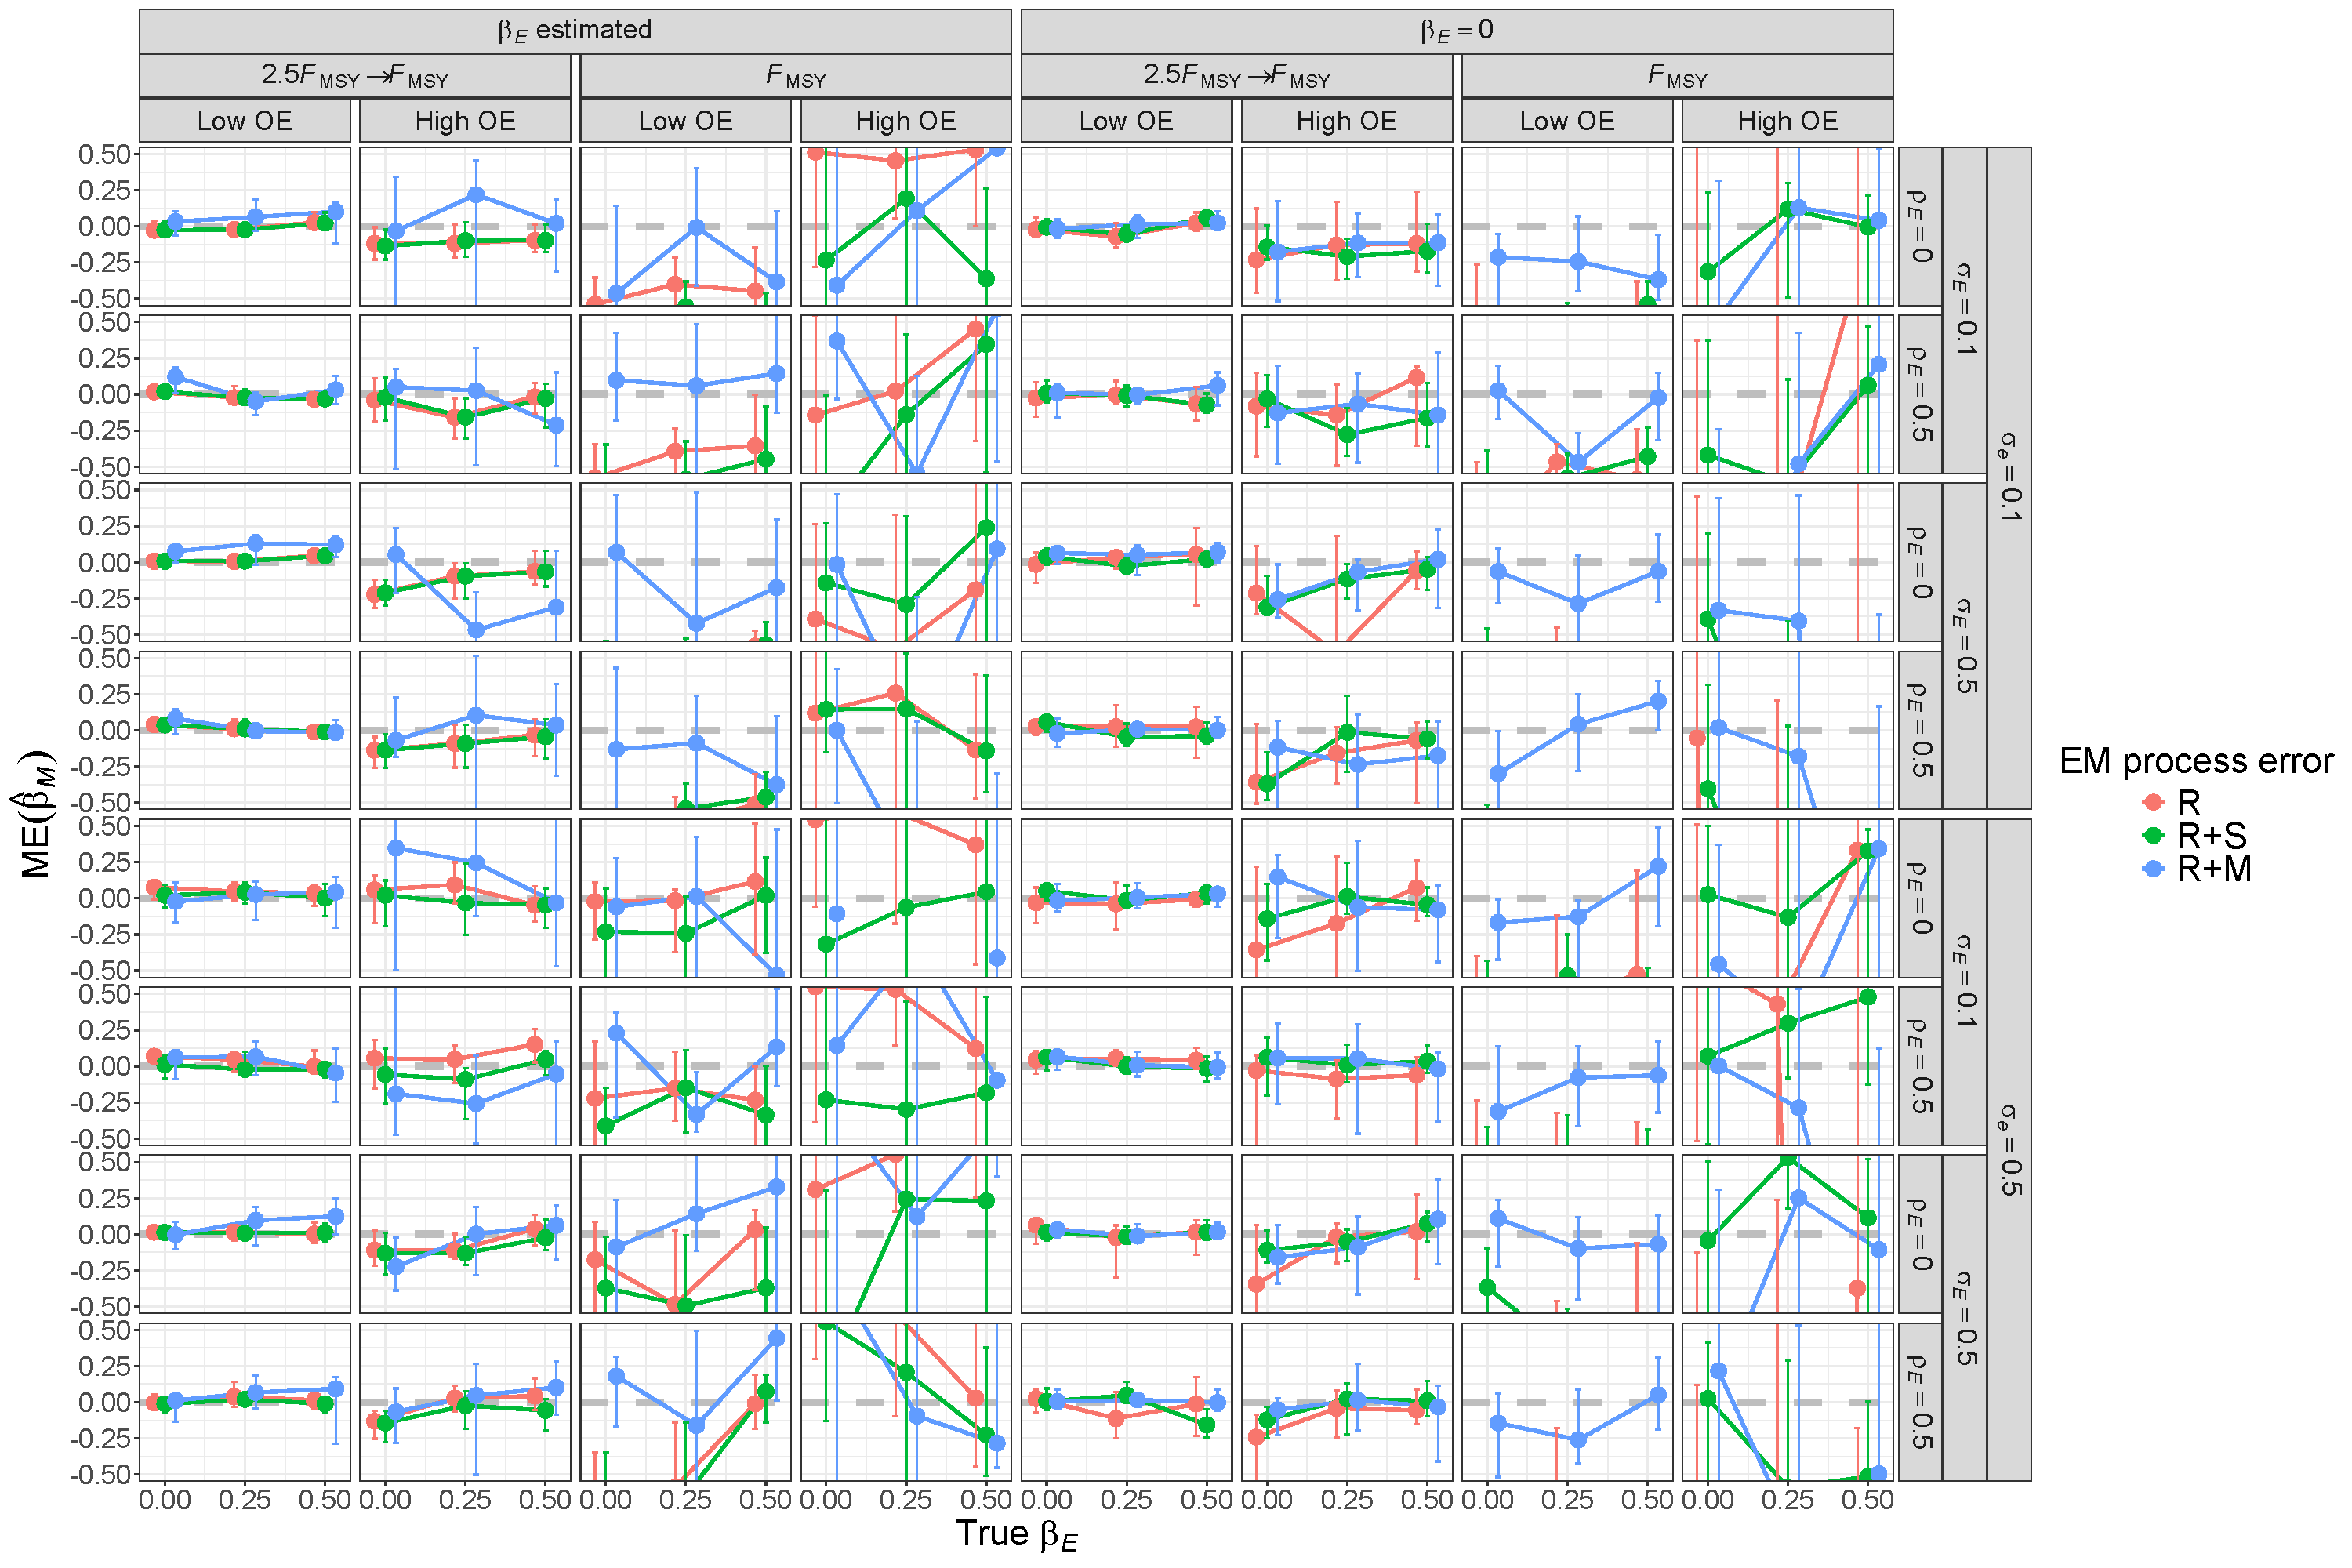
\includegraphics[height = \textheight]{beta_M_bias_RMom}
\end{center}
\caption{\DIFaddFL{For R+M operating models, median error (ME) of estimates of $\beta_M$ from fitting estimating models with alternative process error assumptions and treatment of covariate effect ($\beta_E = 0$ or estimated). Vertical lines represent 95\% confidence intervals.}}\label{beta_M_bias_RMom}
\end{figure}
\end{landscape}

\begin{landscape}
\begin{figure}
\begin{center}
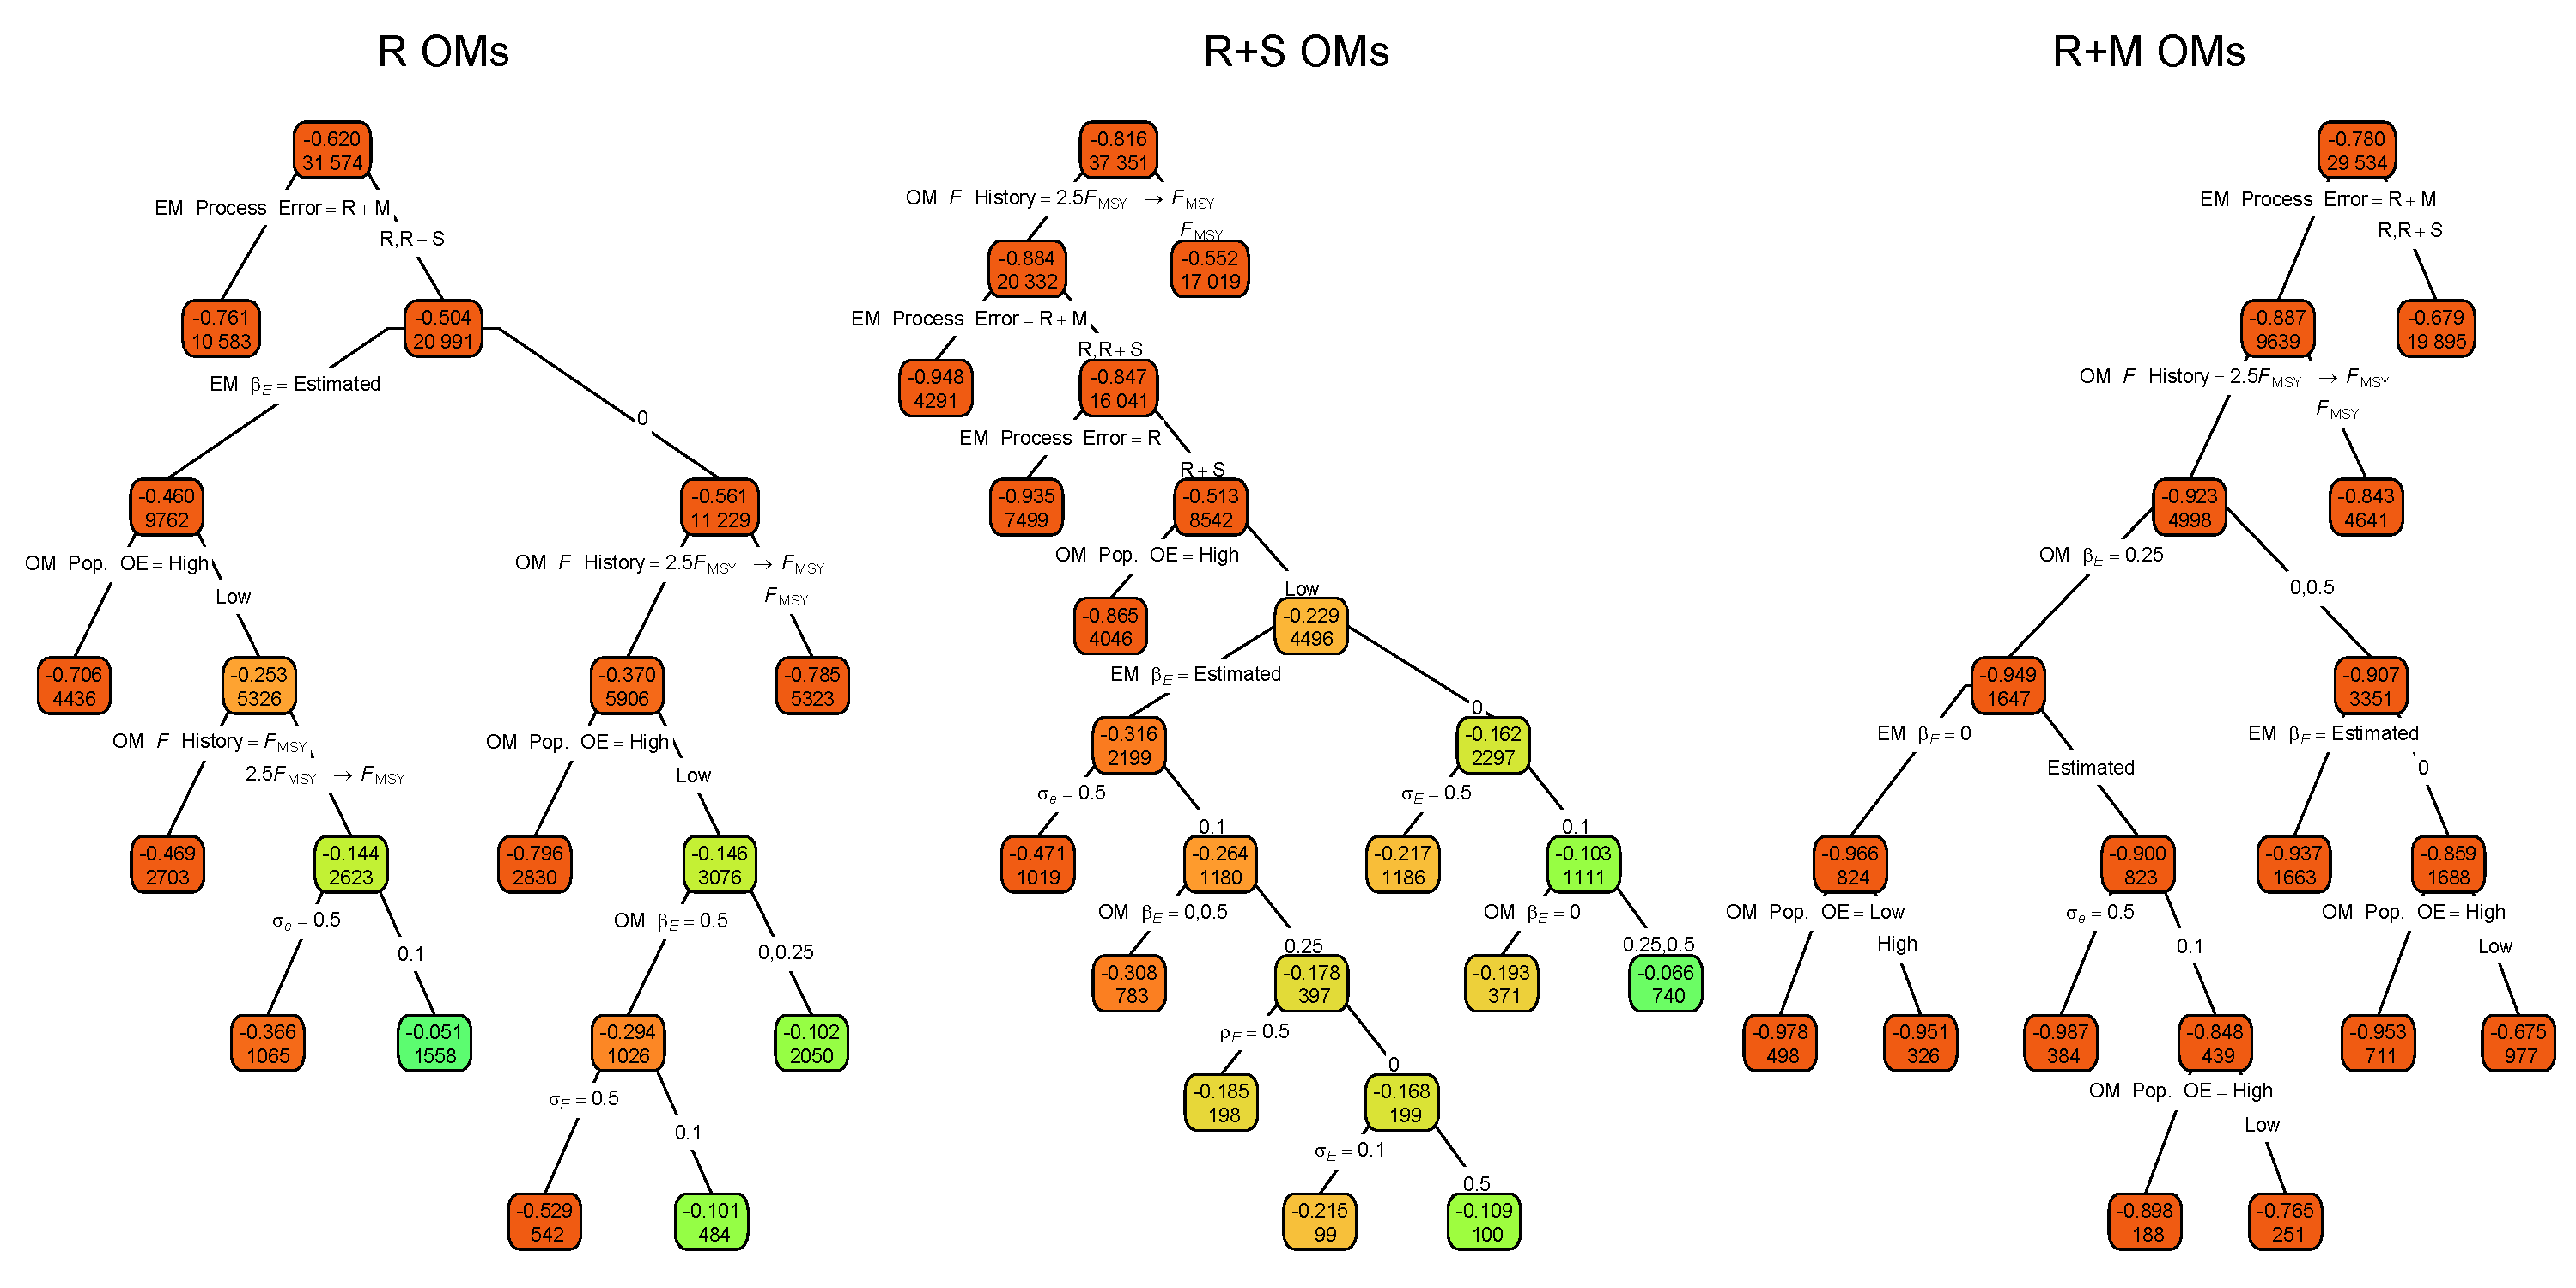
\includegraphics[width = 1.4\textwidth]{median_M_SE_bias_regtree_plots}
\end{center}
\caption{\DIFaddFL{Regression trees for errors of the Hessian-based standard error estimates for median $M$ parameter ($\widehat {\text{SE}}\left(\widehat \beta_M\right)$). Each node shows the median error for the corresponding subset. Lower or higher absolute median absolute errors of the process error assumption are indicated by more green or red polygons, respectively. See Figure \ref{conv_class} caption and Table \ref{factor_table} for further details.}}\label{med_M_SE_bias_regtree}
\end{figure}
\end{landscape}

\begin{landscape}
\begin{figure}
\begin{center}
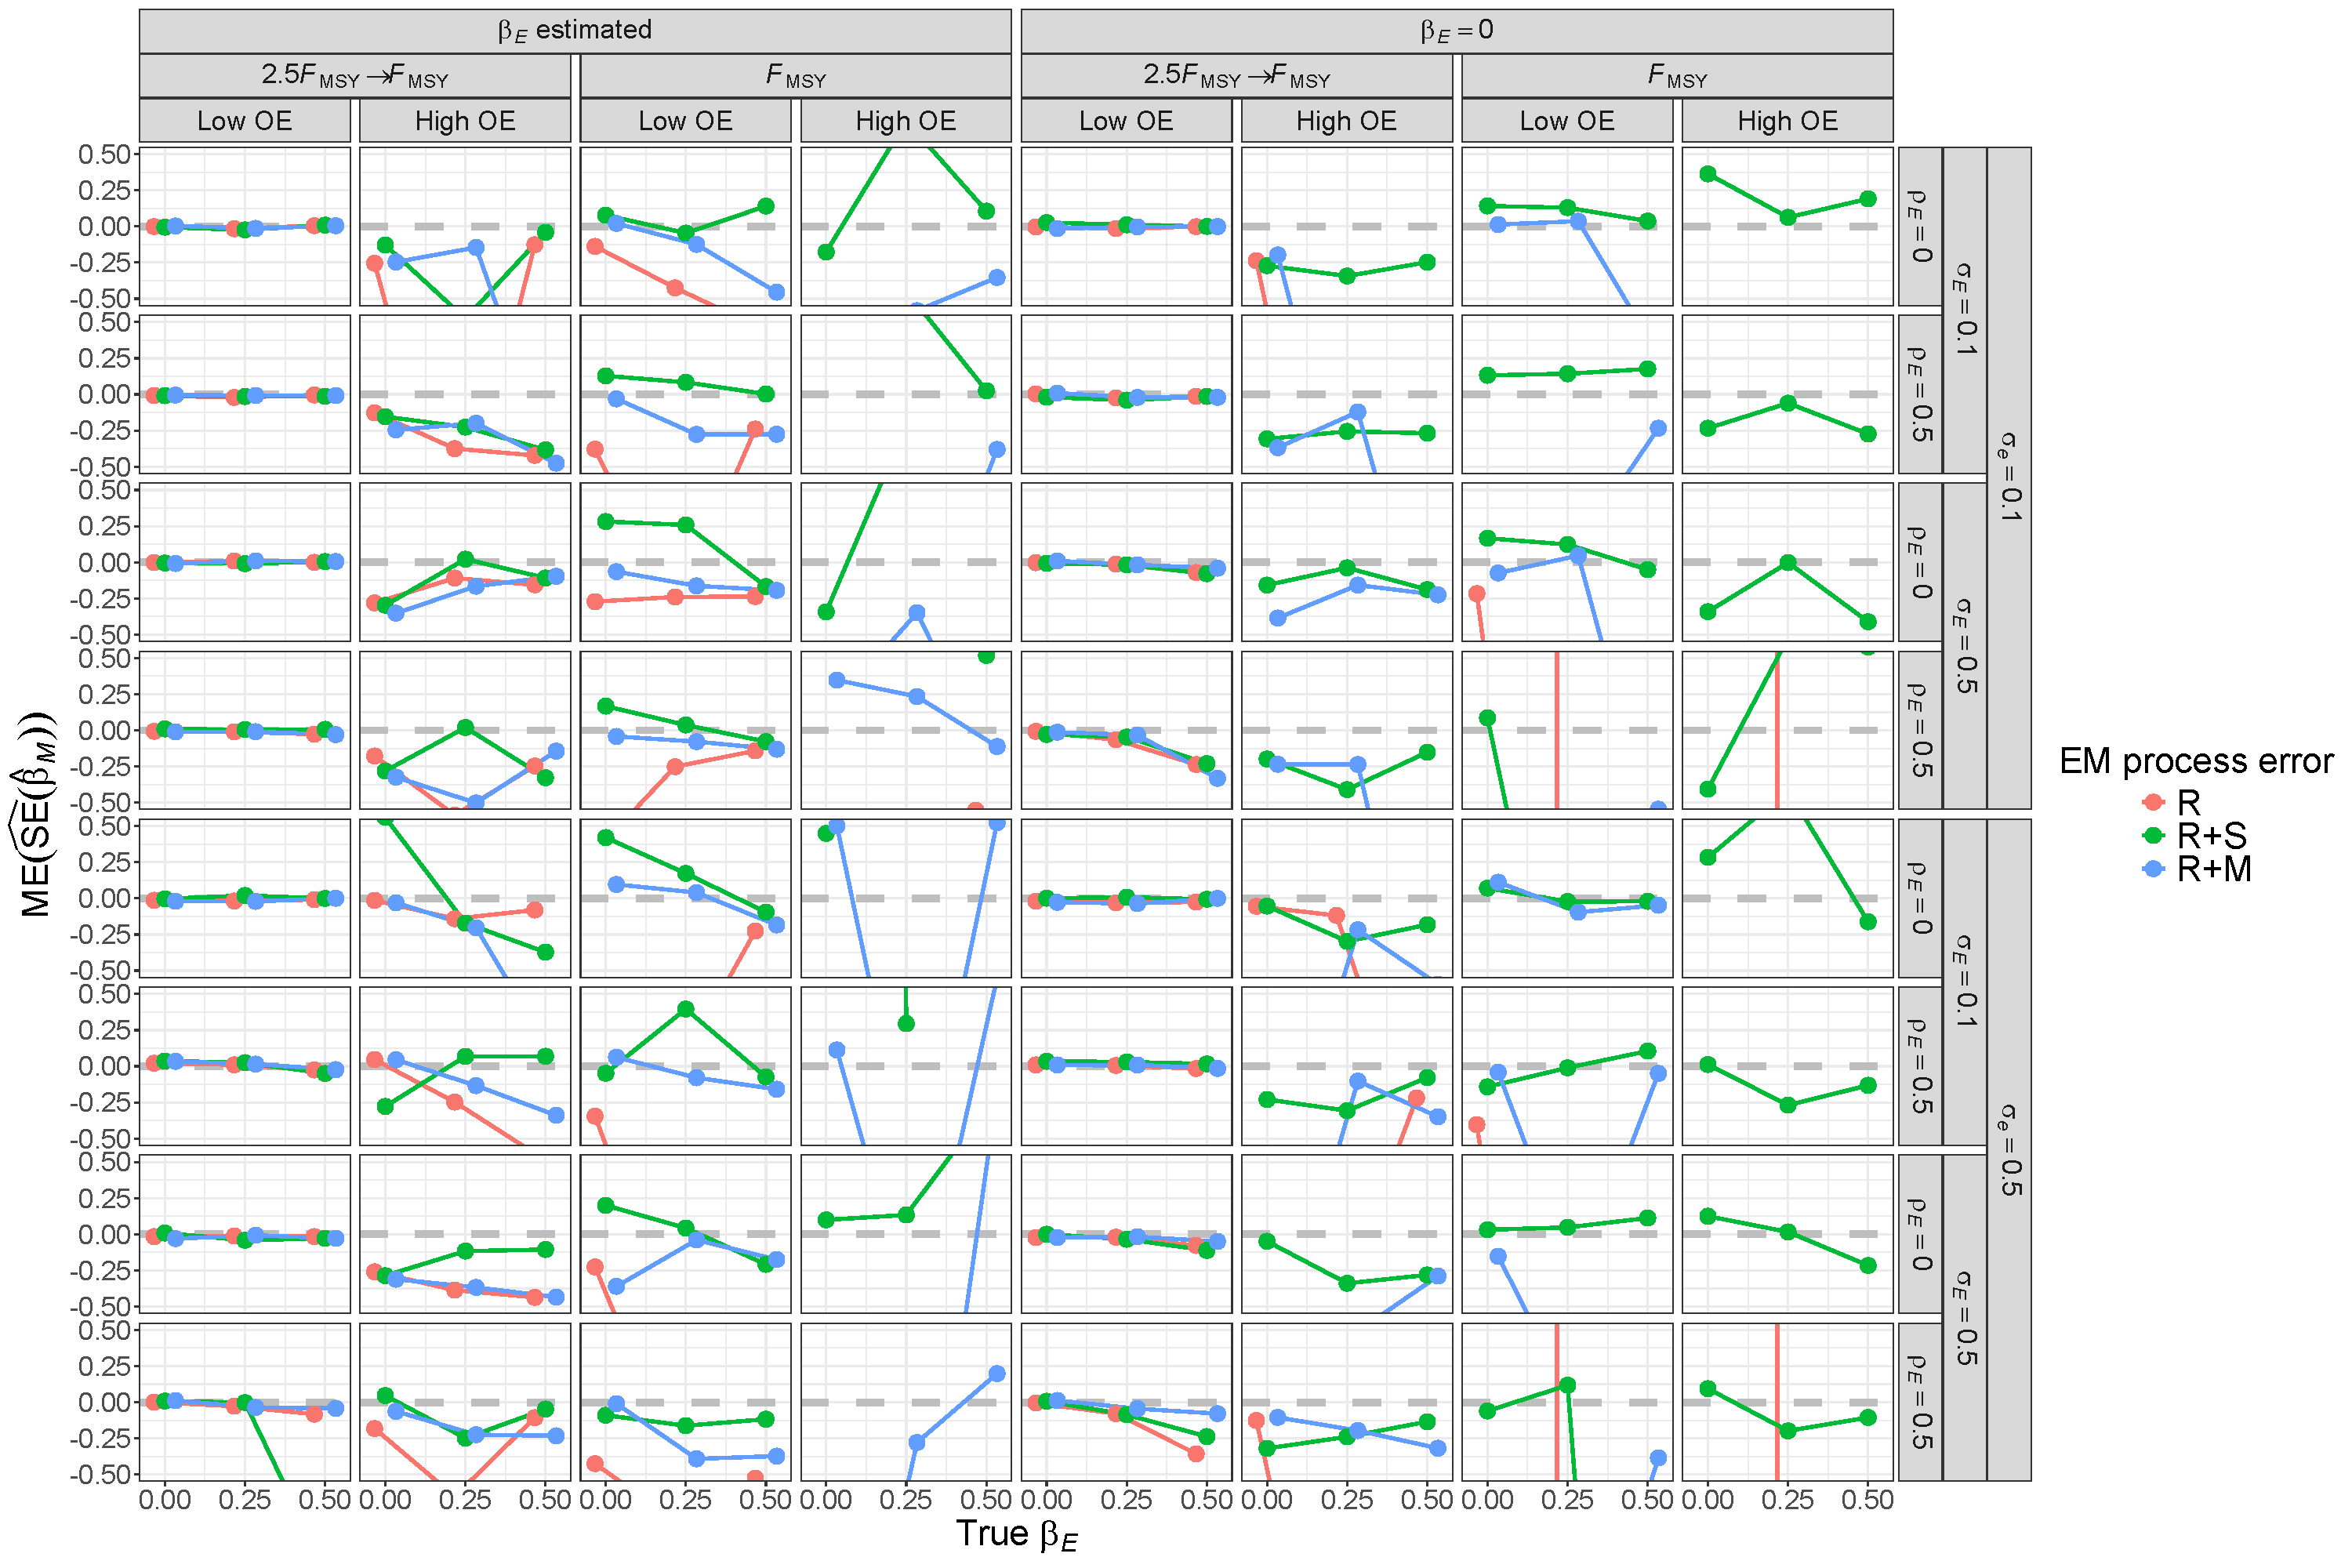
\includegraphics[height = \textheight]{se_beta_M_bias_Rom}
\end{center}
\caption{\DIFaddFL{For R operating models, median error (ME) of Hessian-based estimates of standard error for median $M$ parameter ($\beta_M$) from fitting estimating models with alternative process error assumptions and treatment of the covariate effect ($\beta_ E= 0$ or estimated). True standard error is defined as the mean of the standard error estimates accross converged fits to simulated data sets for a given operating model scenario.}}\label{se_beta_M_bias_Rom}
\end{figure}
\end{landscape}

\begin{landscape}
\begin{figure}
\begin{center}
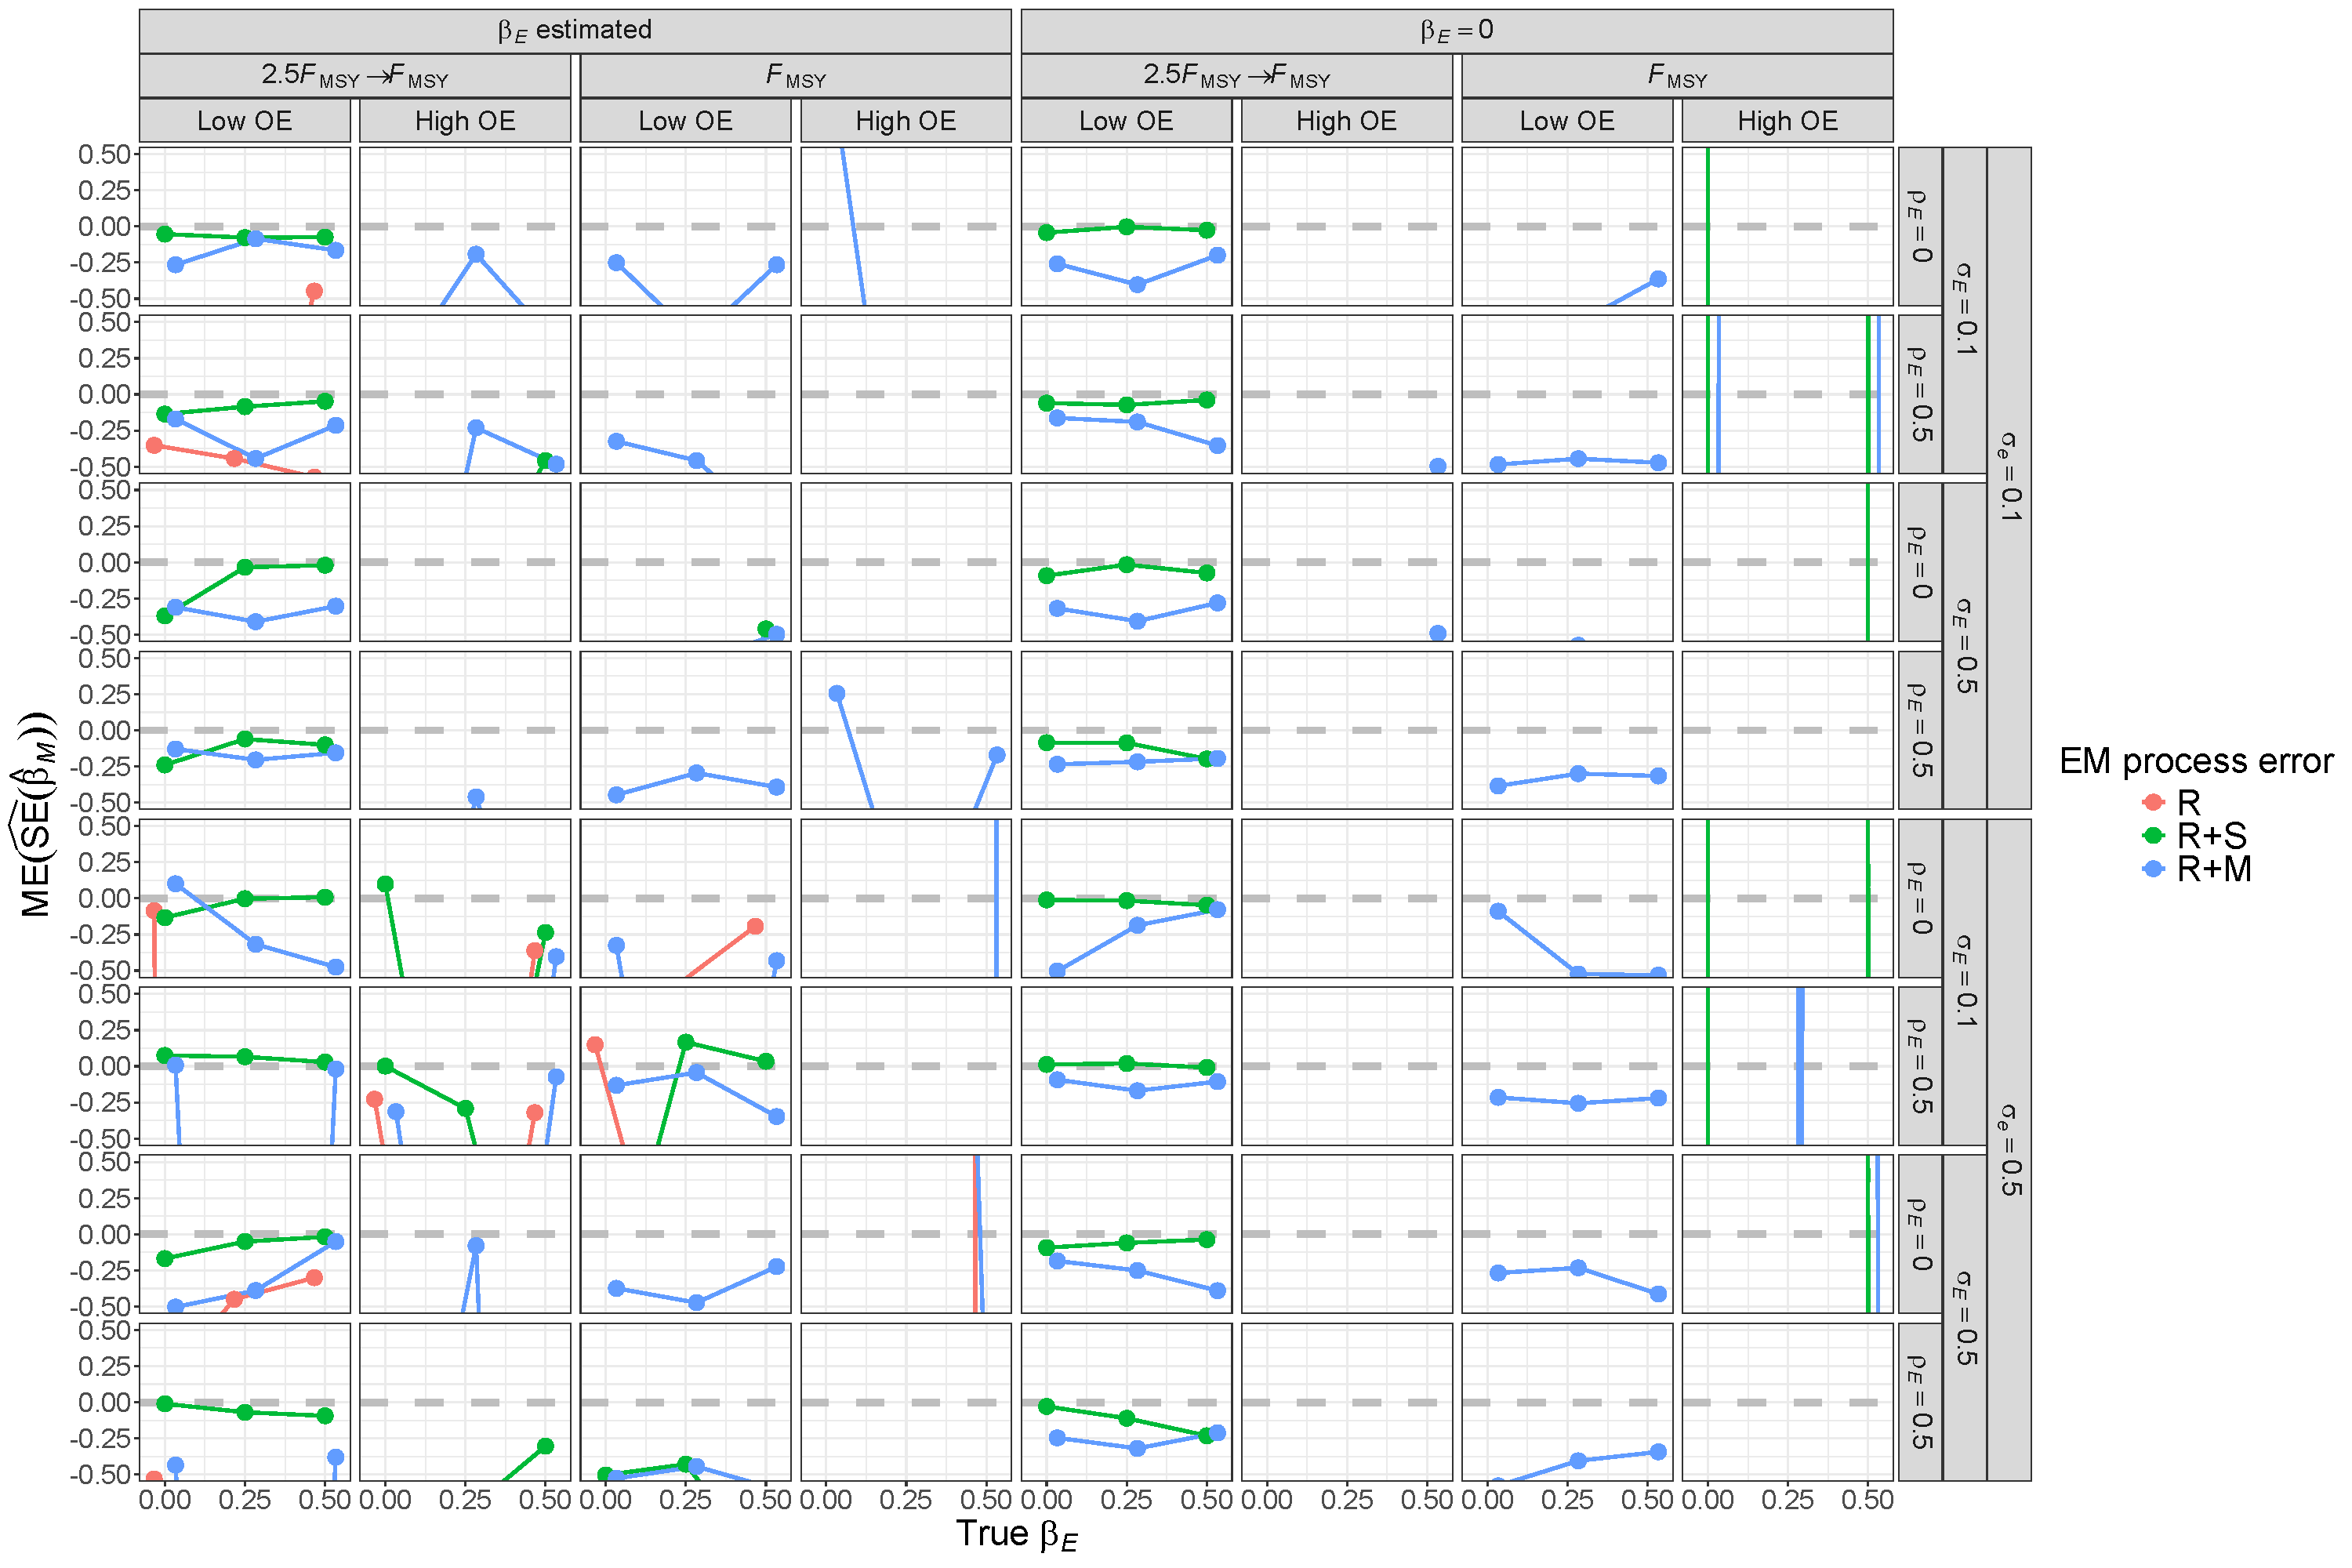
\includegraphics[height = \textheight]{se_beta_M_bias_RSom}
\end{center}
\caption{\DIFaddFL{For R+S operating models, median error (ME) of Hessian-based estimates of standard error for median $M$ parameter ($\beta_M$) from fitting estimating models with alternative process error assumptions and treatment of the covariate effect ($\beta_ E= 0$ or estimated). True standard error is defined as the mean of the standard error estimates accross converged fits to simulated data sets for a given operating model scenario.}}\label{se_beta_M_bias_RSom}
\end{figure}
\end{landscape}

\begin{landscape}
\begin{figure}
\begin{center}
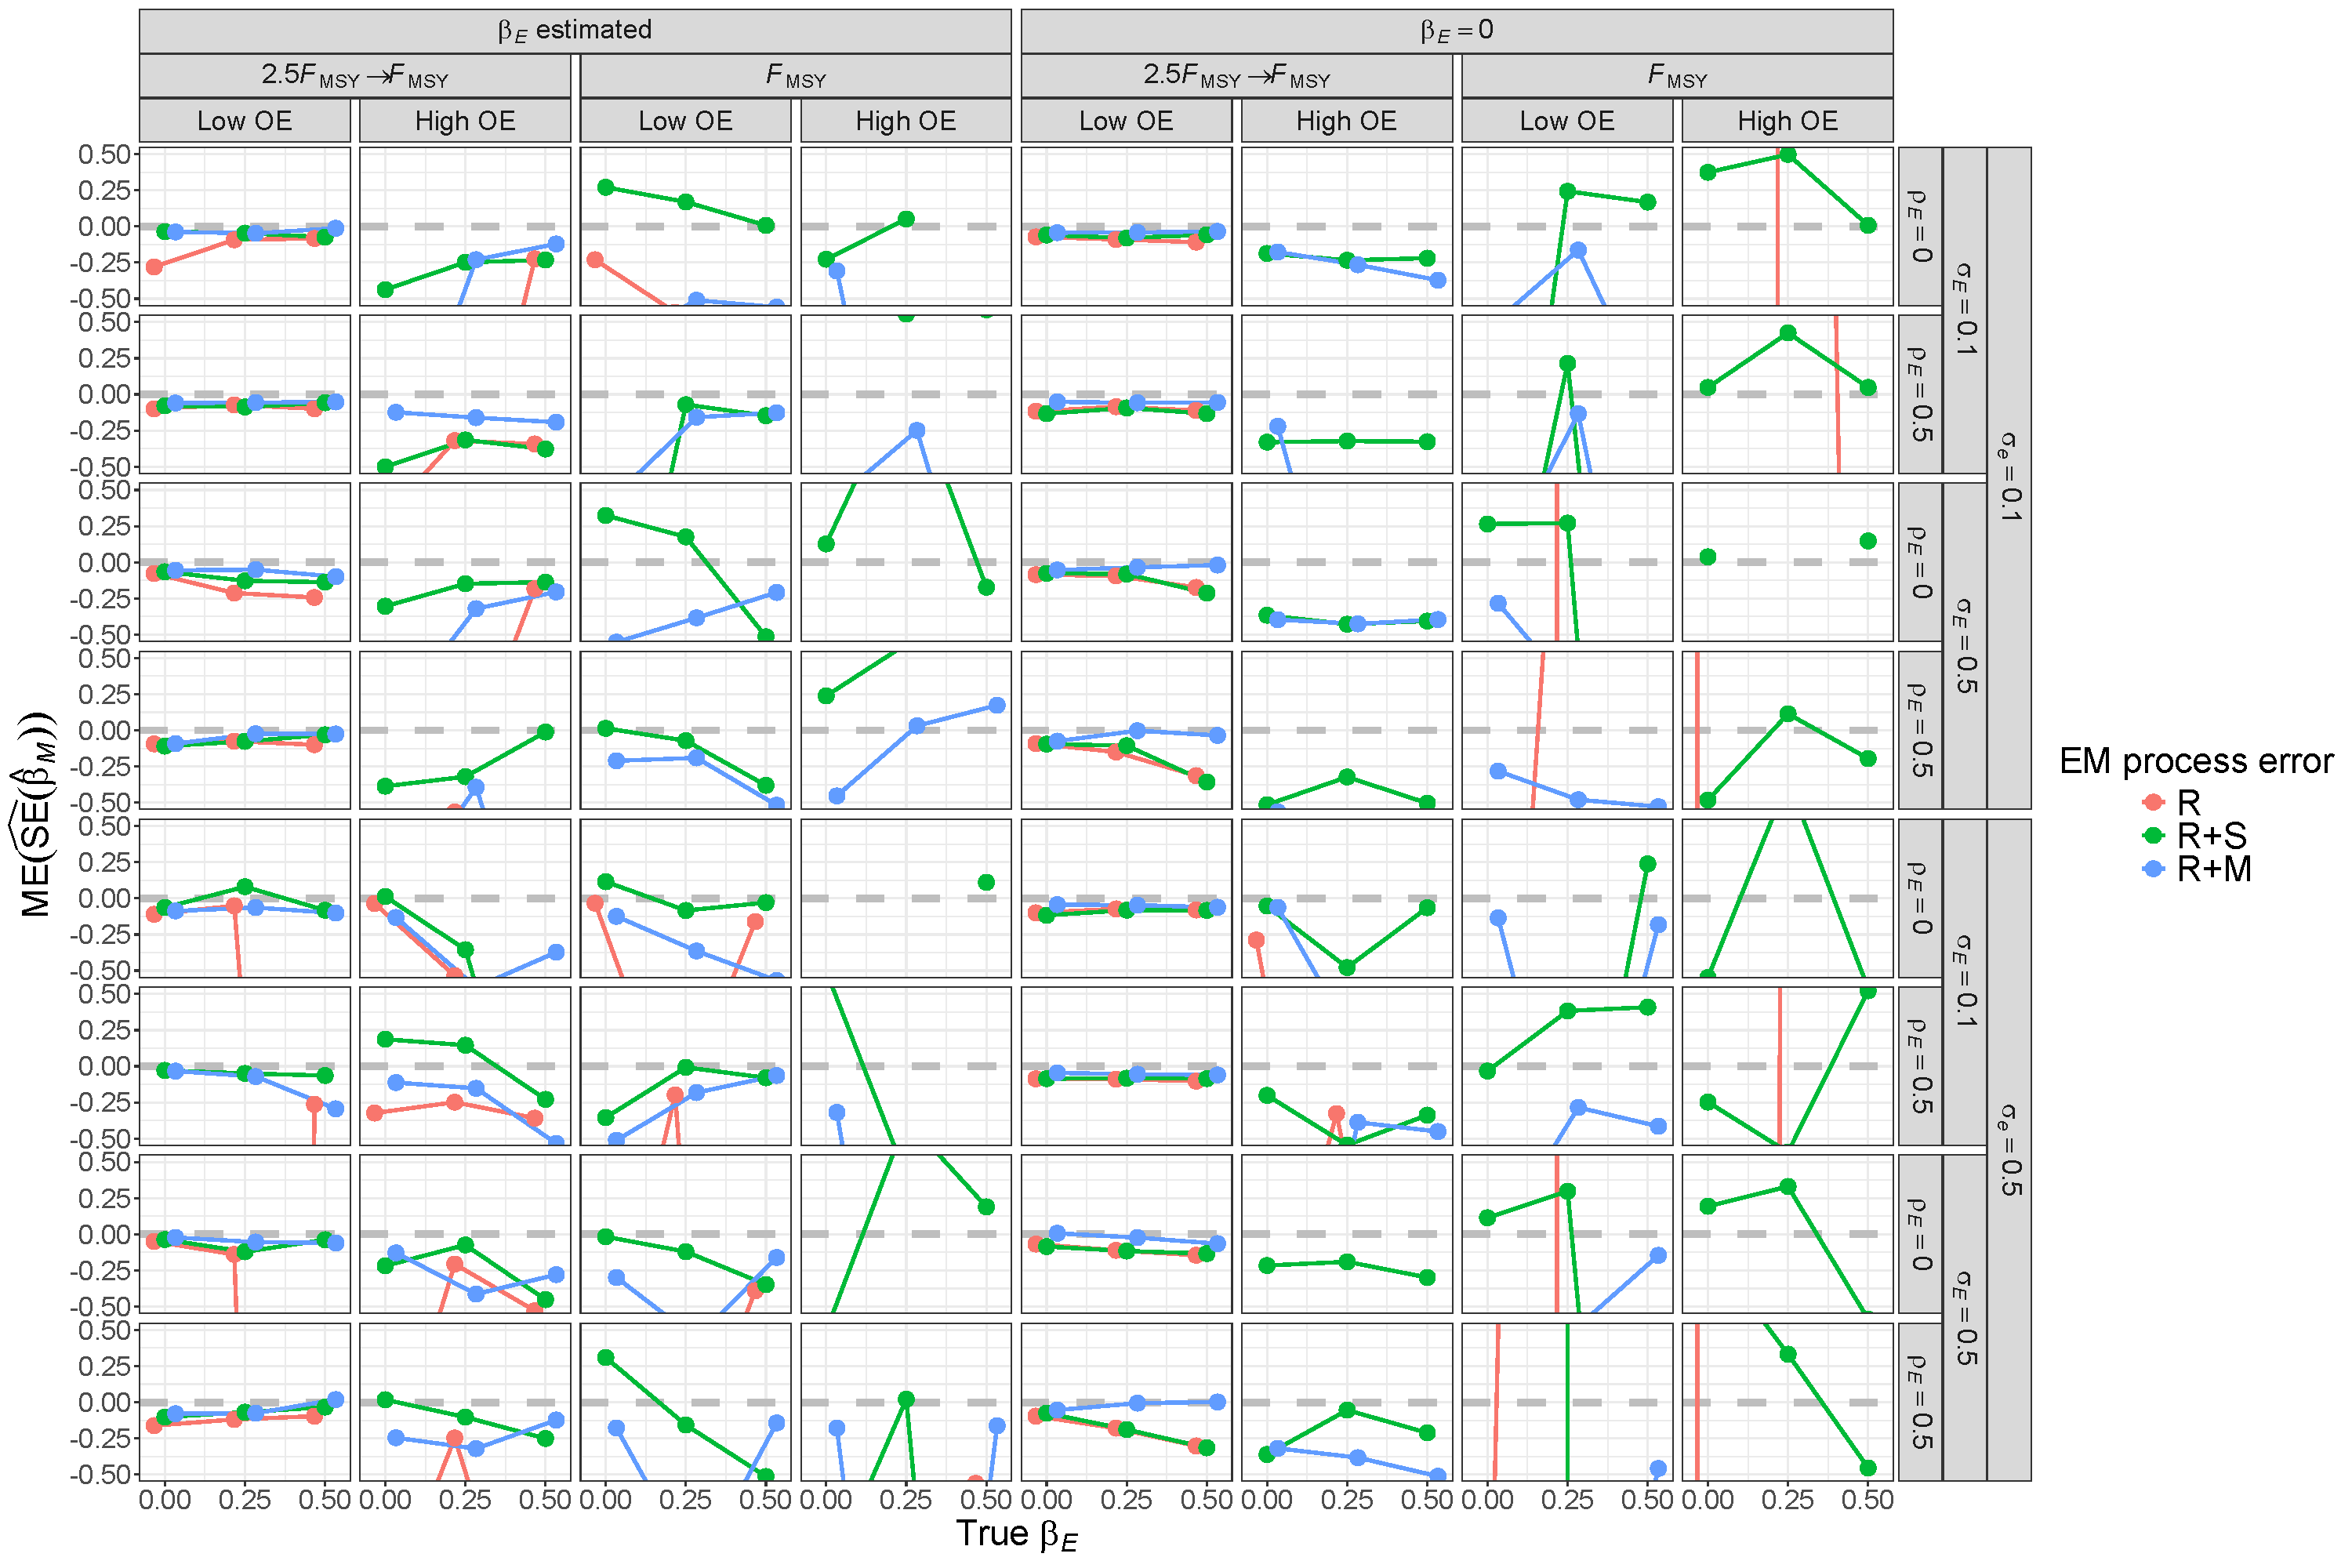
\includegraphics[height = \textheight]{se_beta_M_bias_RMom}
\end{center}
\caption{\DIFaddFL{For R+M operating models, median error (ME) of Hessian-based estimates of standard error for median $M$ parameter ($\beta_M$) from fitting estimating models with alternative process error assumptions and treatment of the covariate effect ($\beta_ E= 0$ or estimated). True standard error is defined as the mean of the standard error estimates accross converged fits to simulated data sets for a given operating model scenario.}}\label{se_beta_M_bias_RMom}
\end{figure}
\end{landscape}

\begin{landscape}
\begin{figure}
\begin{center}
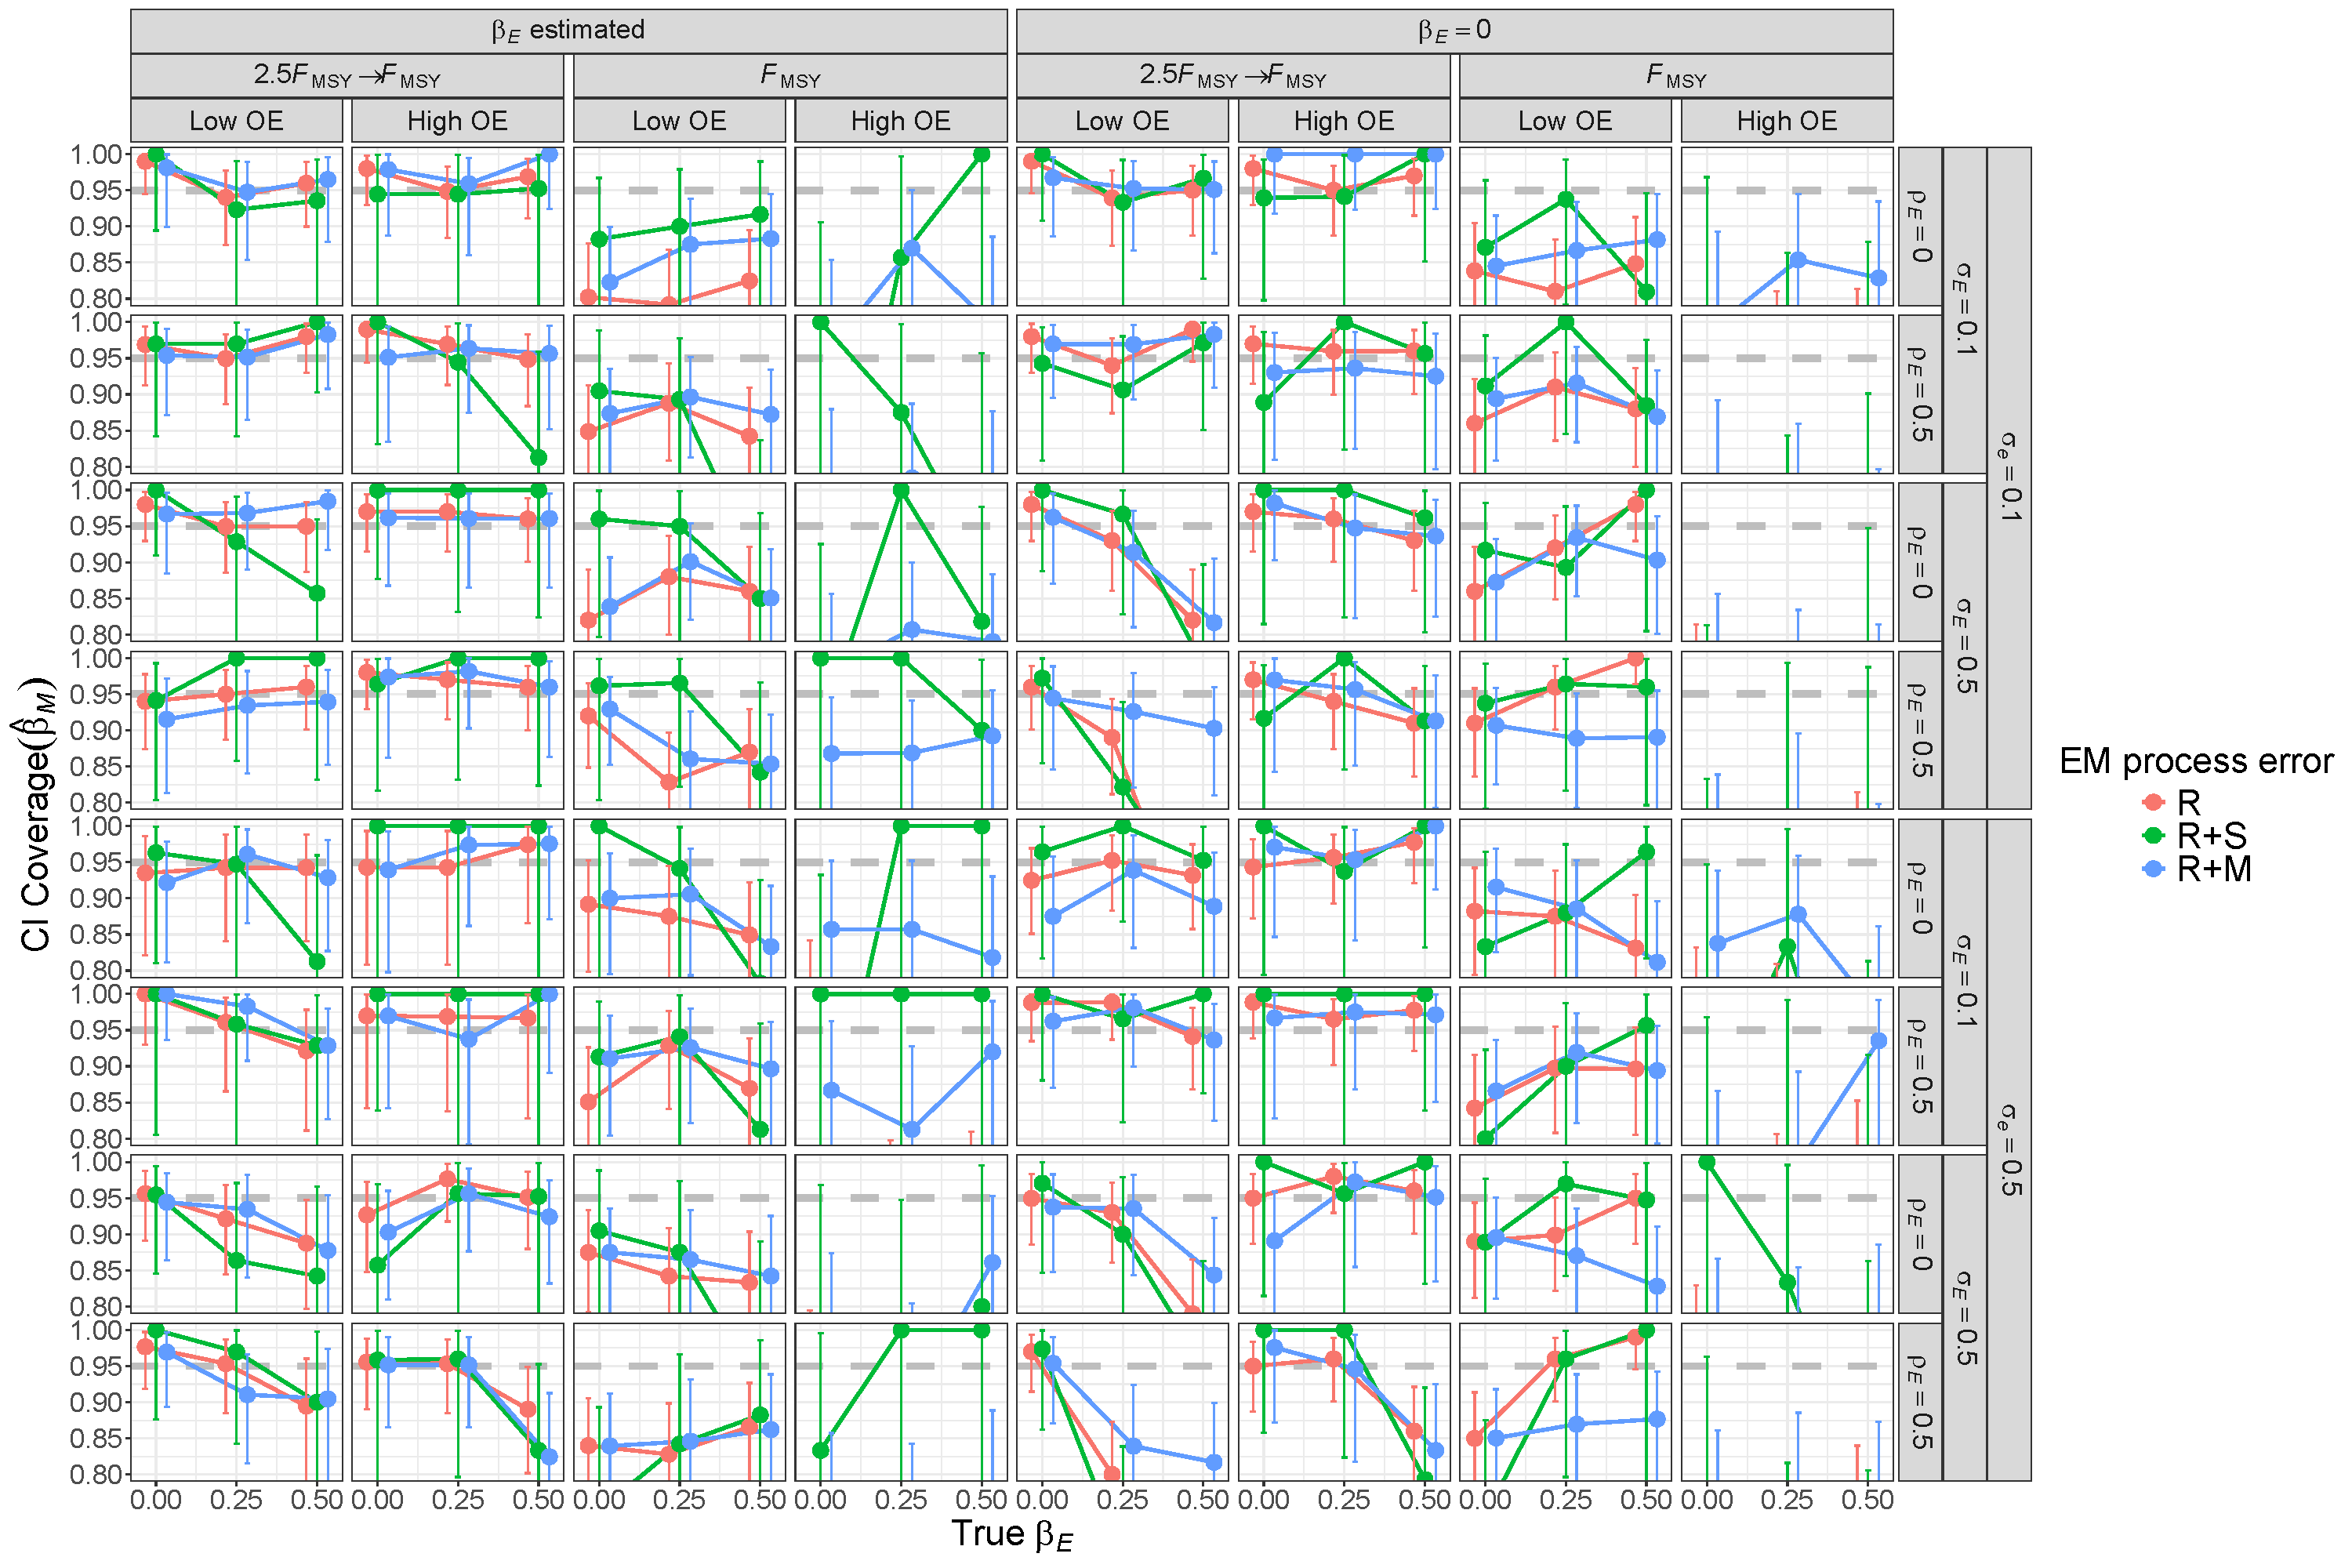
\includegraphics[height = \textheight]{beta_M_CI_coverage_Rom}
\end{center}
\caption{\DIFaddFL{For R operating models, probability of 95\% confidence interval for $\beta_M$ containing the true value for estimating models with alternative process error assumptions and treatment of covariate effect ($\beta_E = 0$ or estimated). Vertical lines represent 95\% confidence intervals.}}\label{beta_M_CI_coverage_Rom}
\end{figure}
\end{landscape}

\begin{landscape}
\begin{figure}
\begin{center}
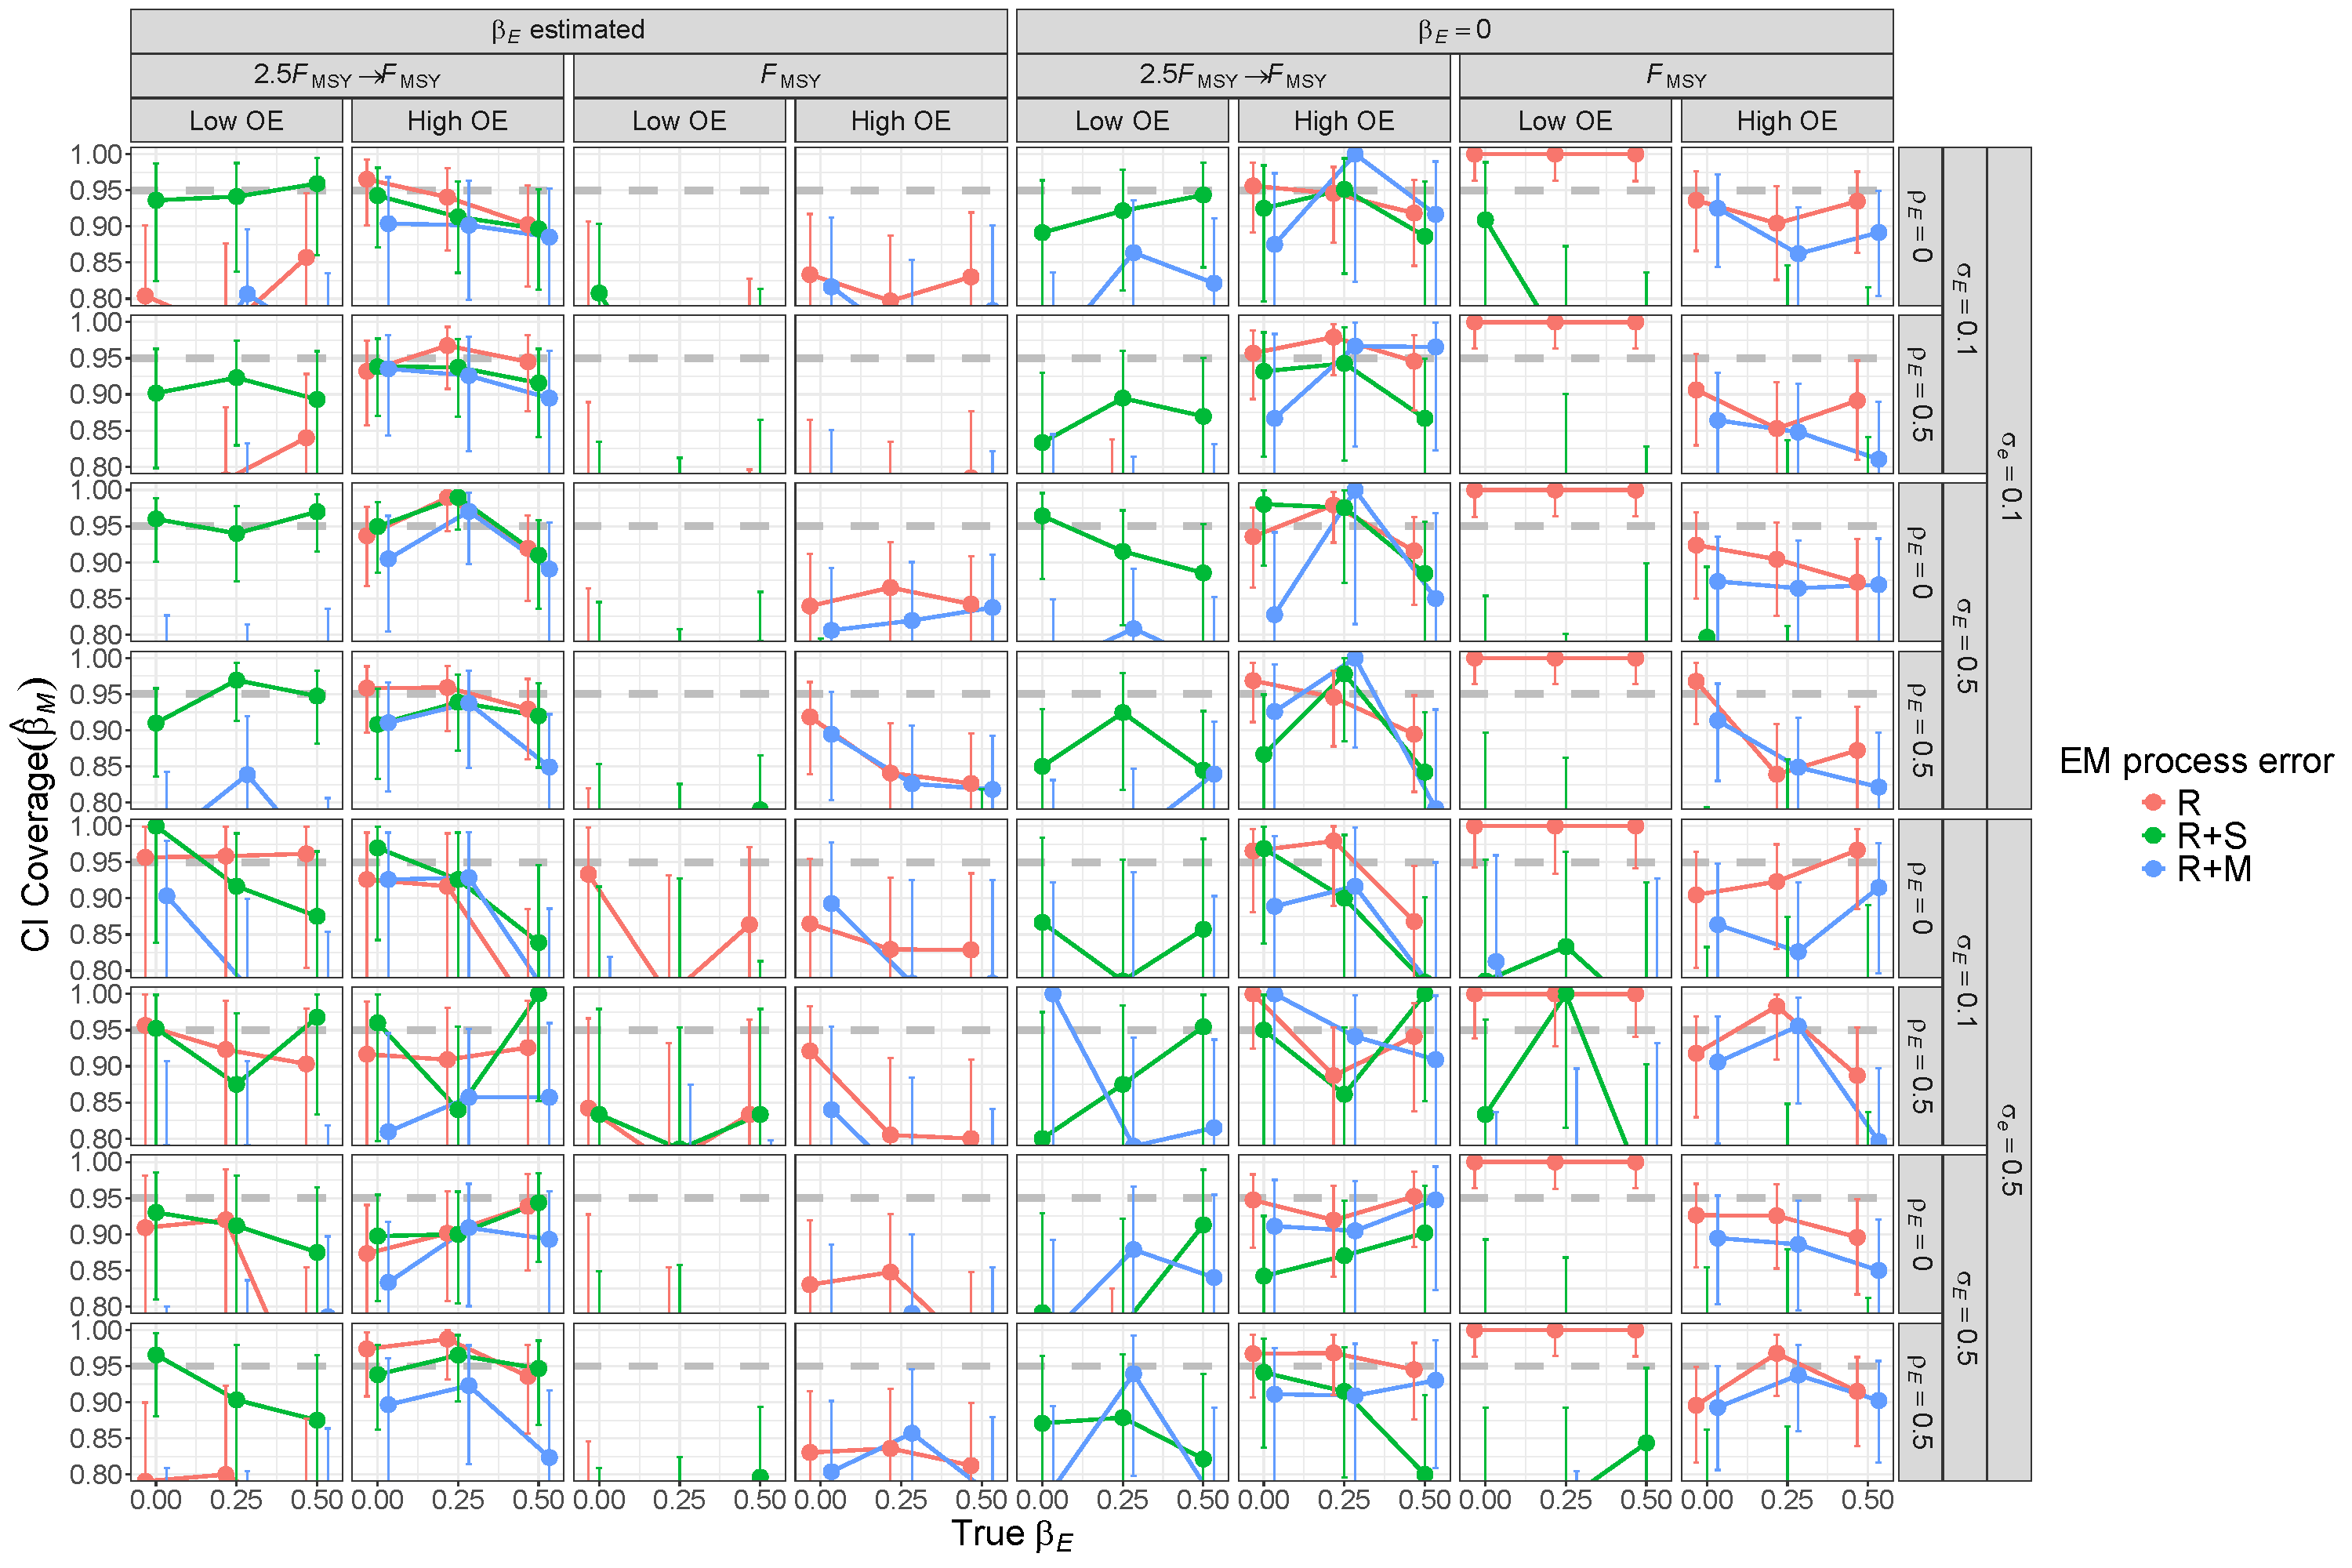
\includegraphics[height = \textheight]{beta_M_CI_coverage_RSom}
\end{center}
\caption{\DIFaddFL{For R+S operating models, probability of 95\% confidence interval for $\beta_M$ containing the true value for estimating models with alternative process error assumptions and treatment of covariate effect ($\beta_E = 0$ or estimated). Vertical lines represent 95\% confidence intervals.}}\label{beta_M_CI_coverage_RSom}
\end{figure}
\end{landscape}

\begin{landscape}
\begin{figure}
\begin{center}
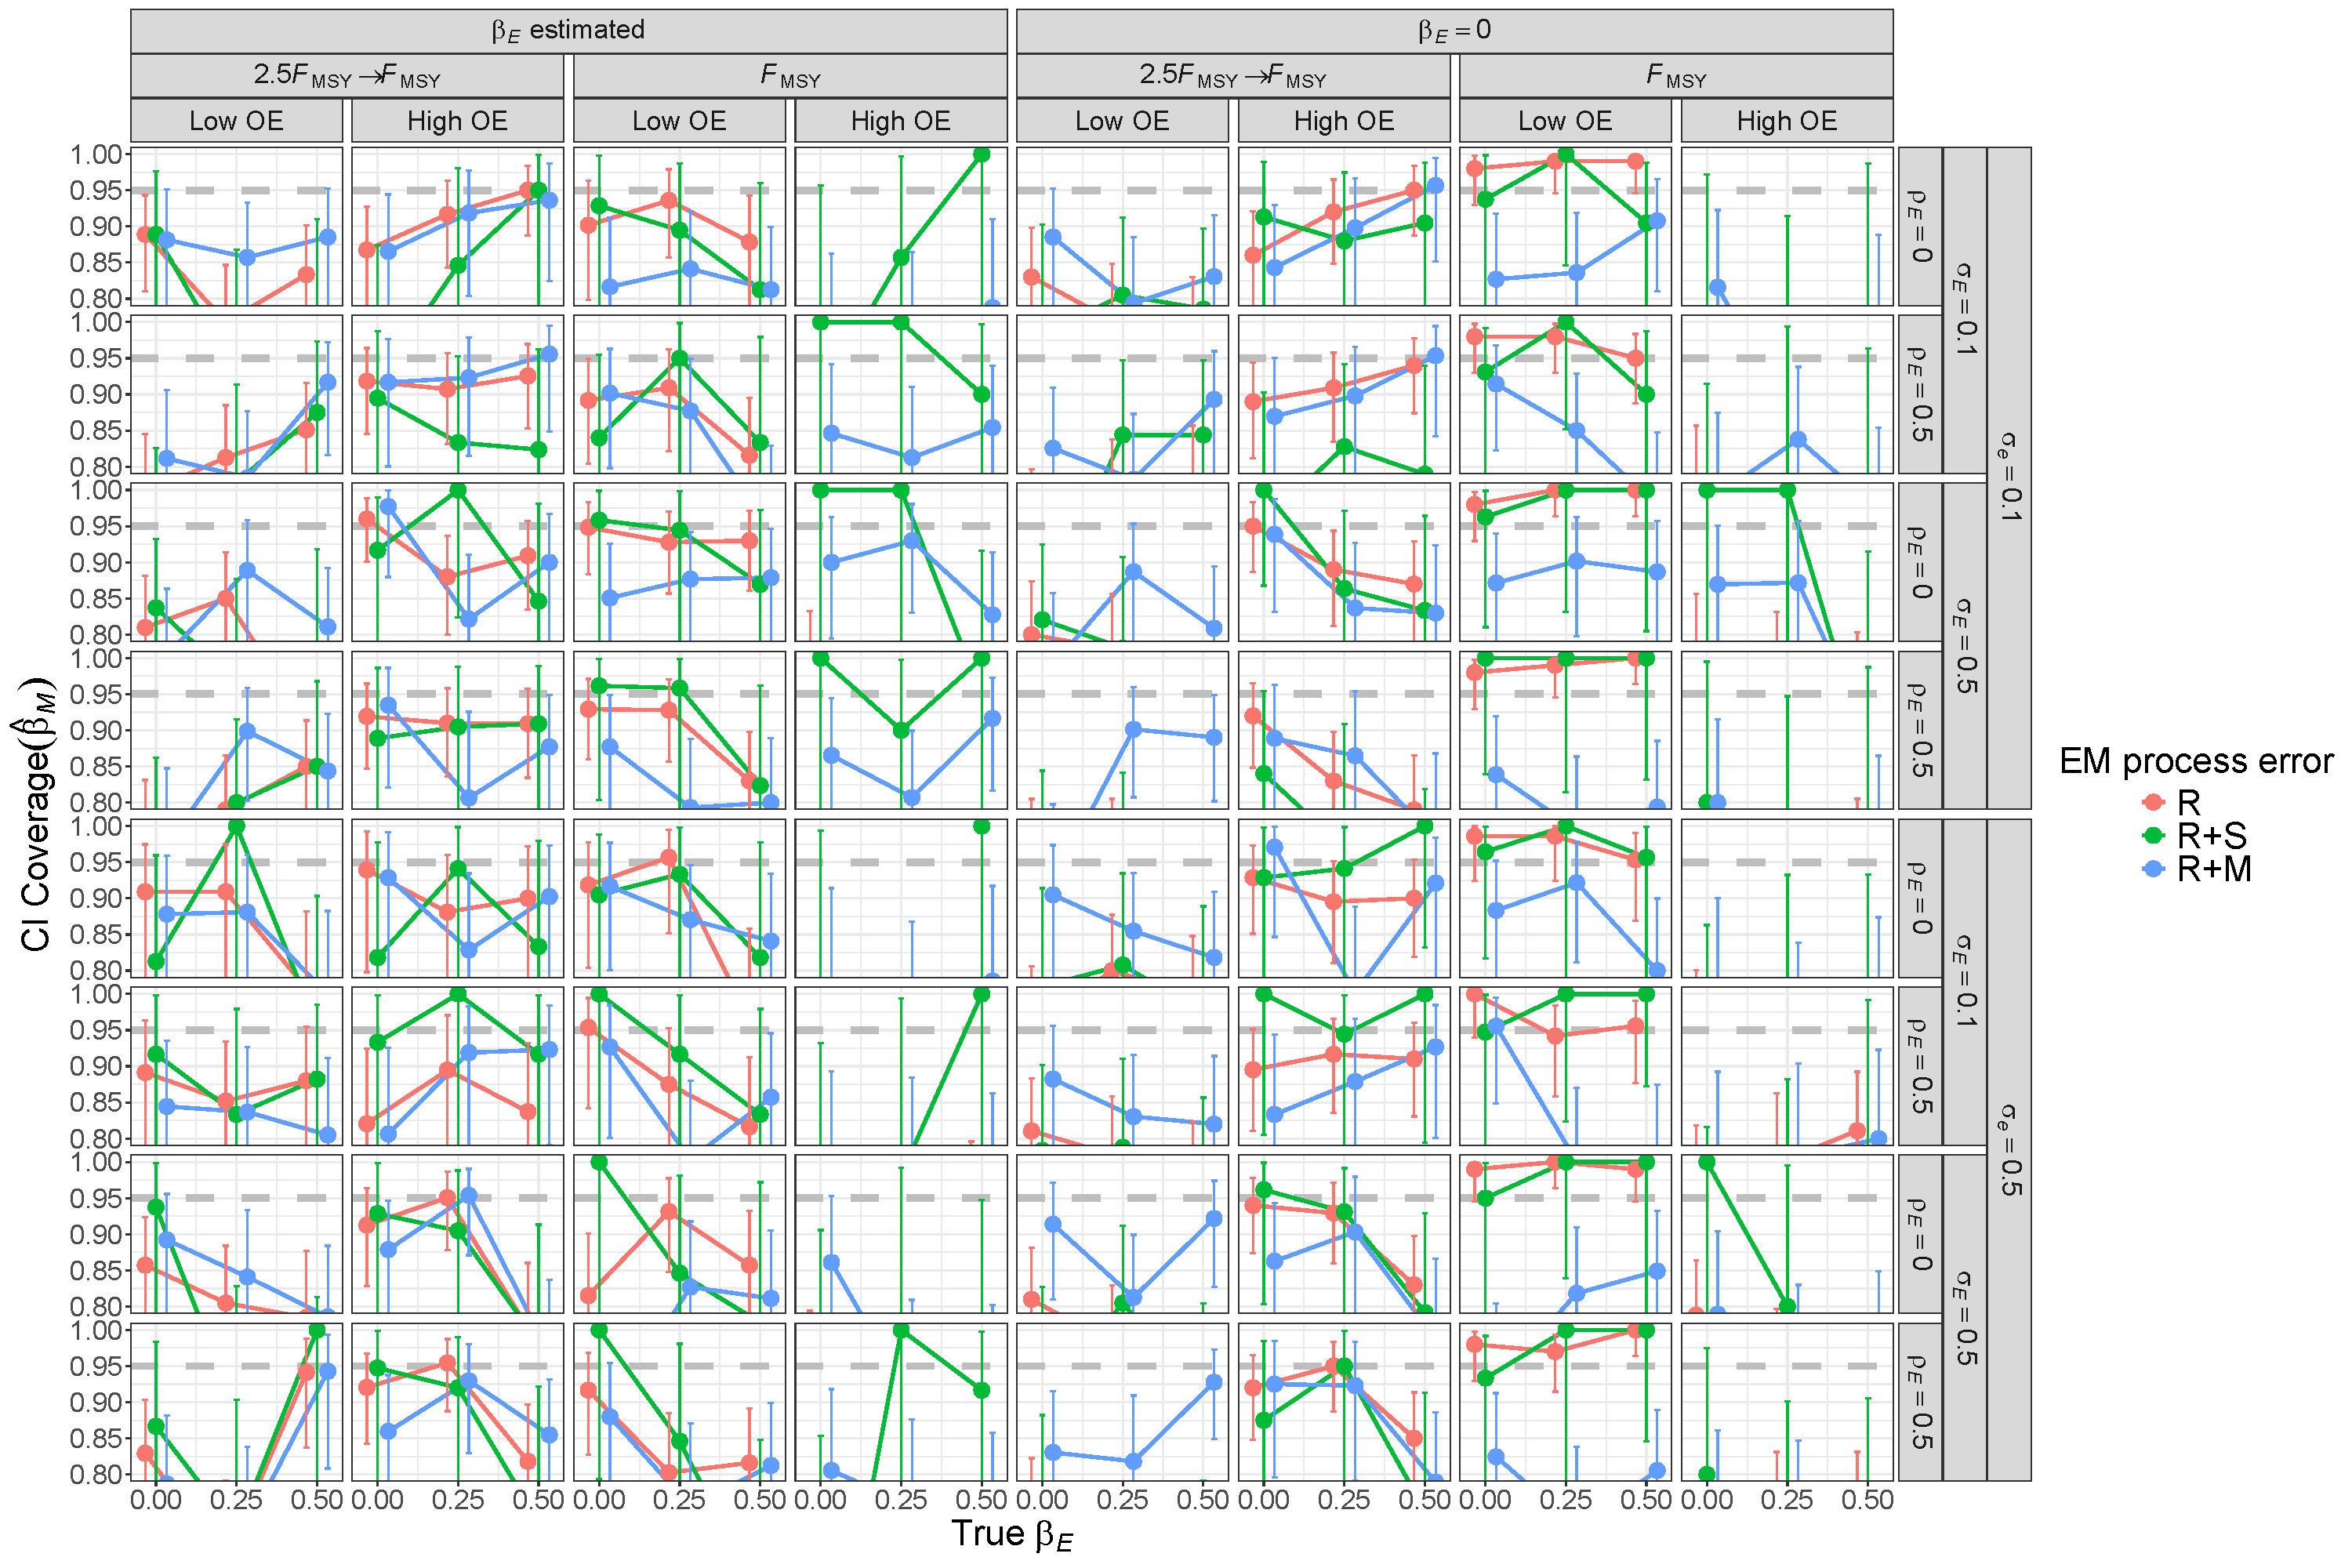
\includegraphics[height = \textheight]{beta_M_CI_coverage_RMom}
\end{center}
\caption{\DIFaddFL{For R+M operating models, probability of 95\% confidence interval for $\beta_M$ containing the true value for estimating models with alternative process error assumptions and treatment of covariate effect ($\beta_E = 0$ or estimated). Vertical lines represent 95\% confidence intervals.}}\label{beta_M_CI_coverage_RMom}
\end{figure}
\end{landscape}

\begin{landscape}
\begin{figure}
\begin{center}
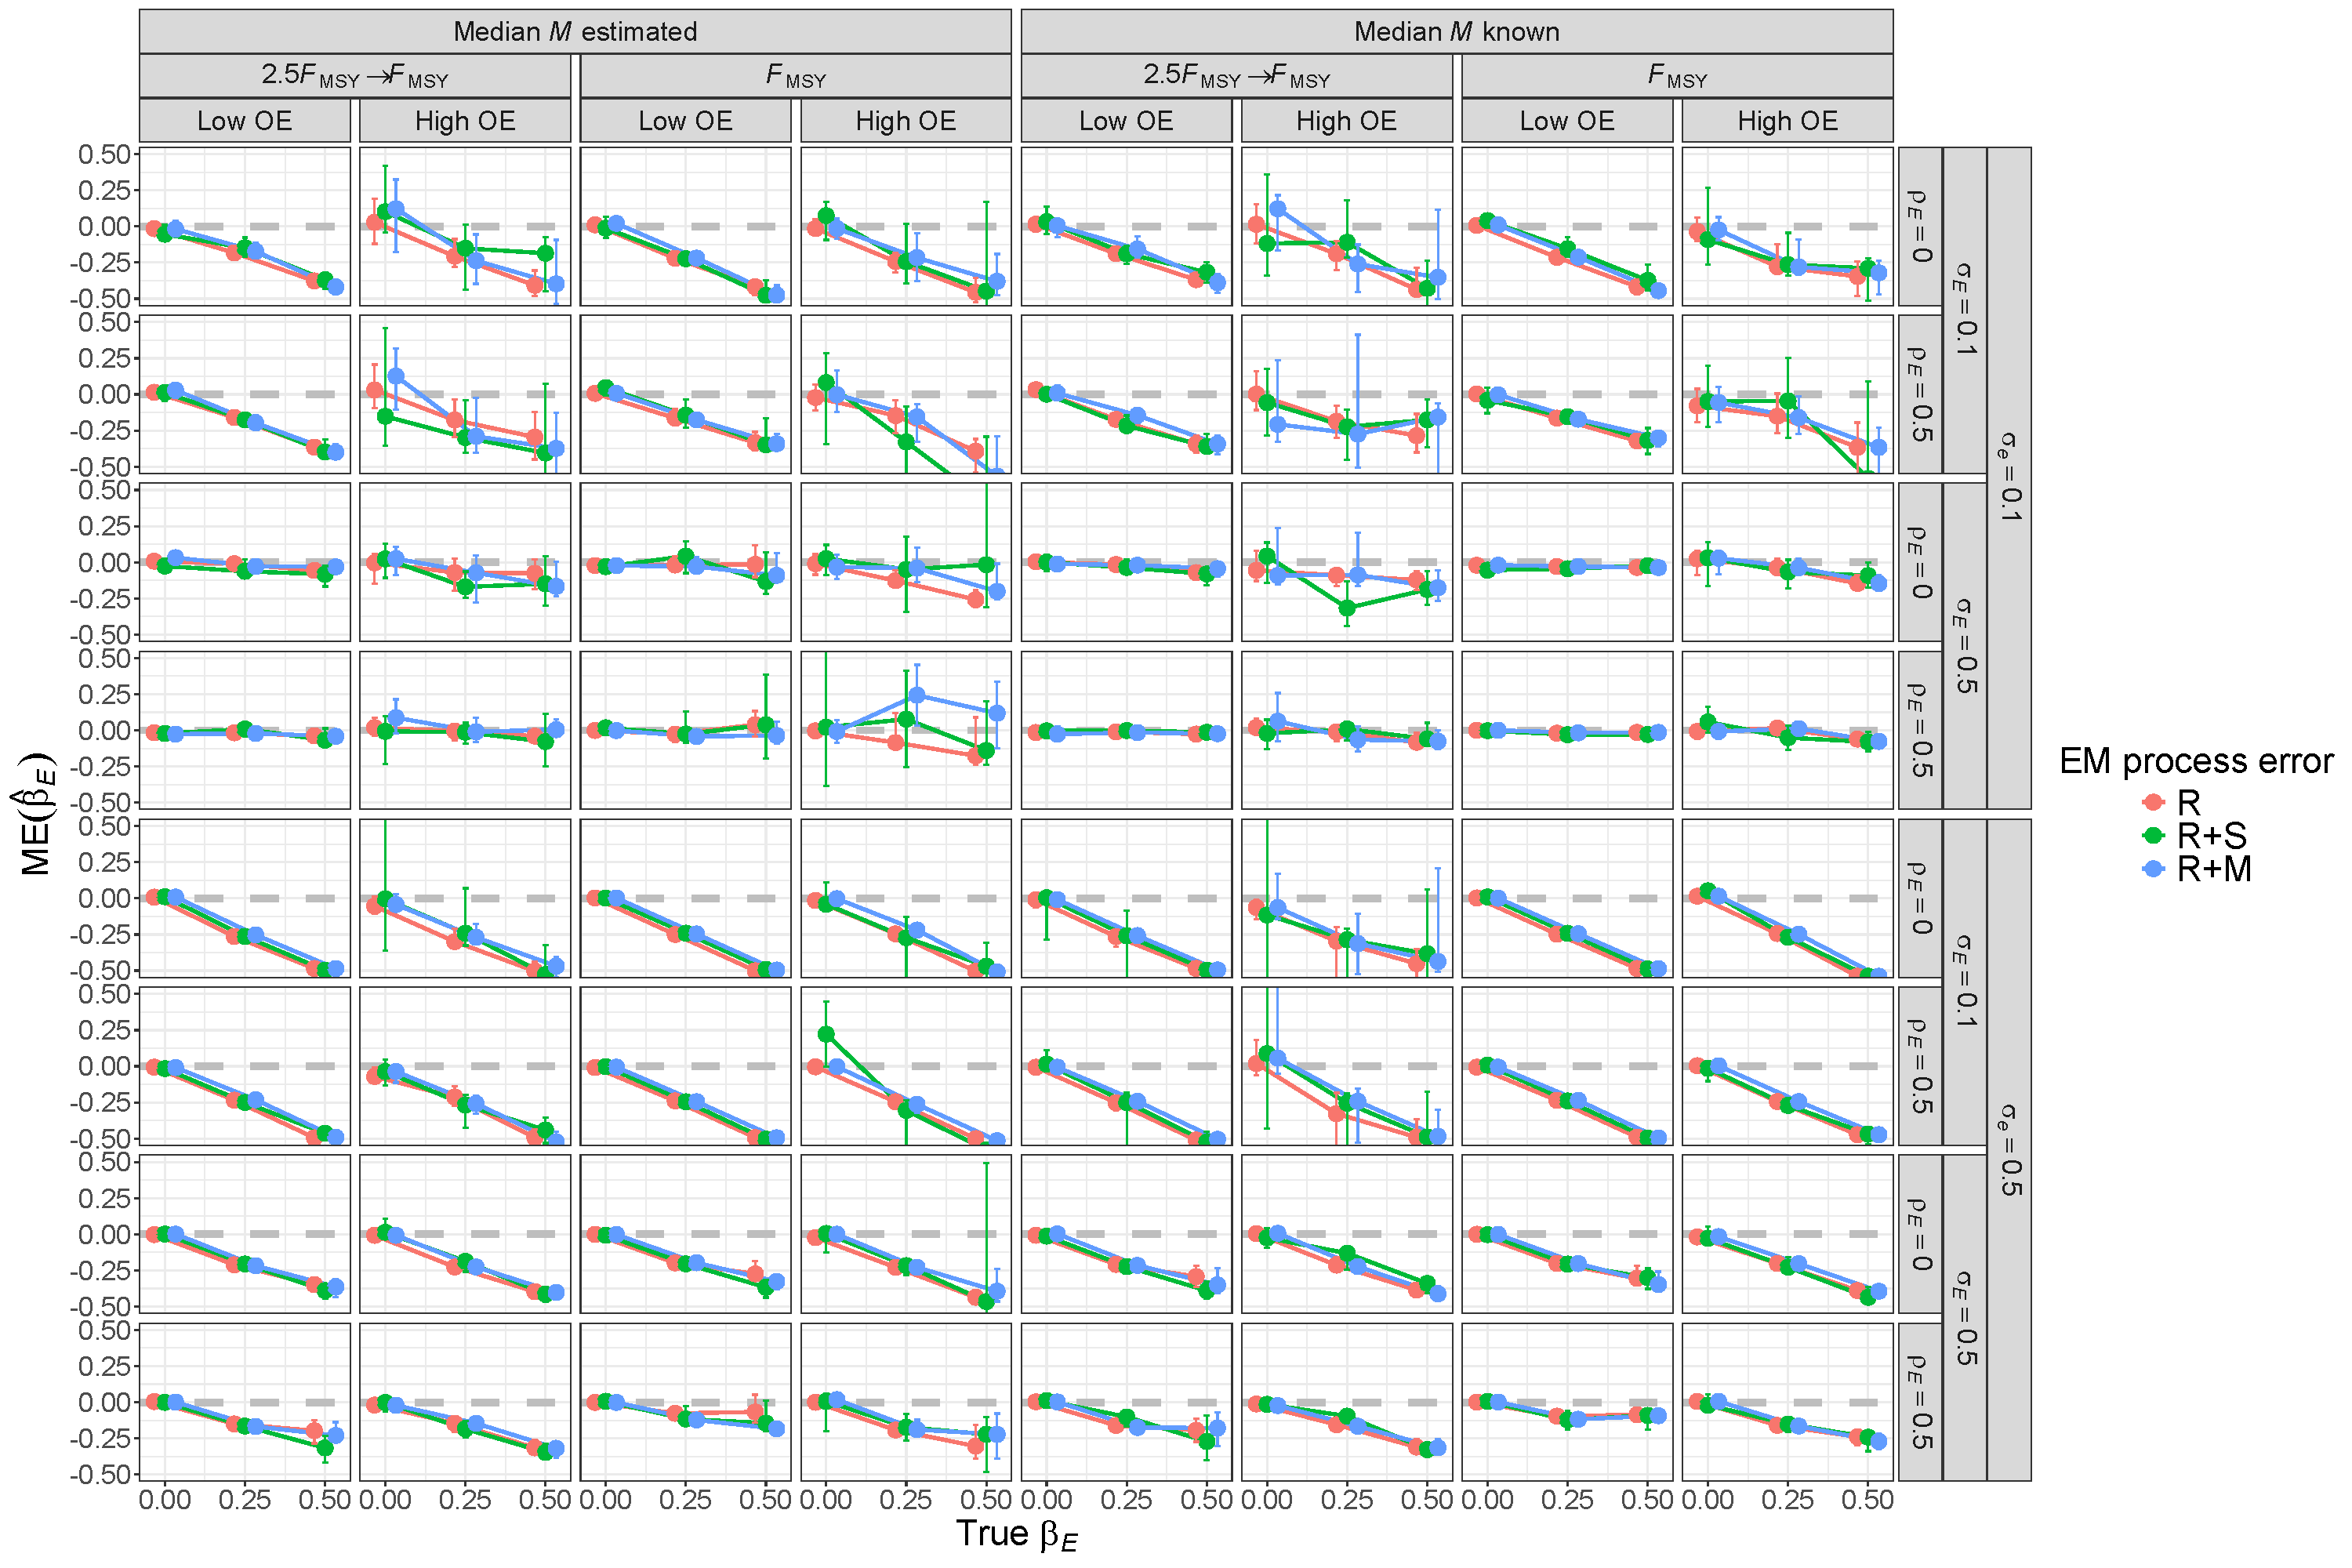
\includegraphics[height = \textheight]{beta_E_bias_Rom}
\end{center}
\caption{\DIFaddFL{For R operating models, median error (ME) of estimates of environmental effect on $M$ ($\beta_E$) from fitting estimating models with alternative process error assumptions and treatment of median $M$ parameter ($\beta_M$). Vertical lines represent 95\% confidence intervals.}}\label{beta_E_bias_Rom}
\end{figure}
\end{landscape}

\begin{landscape}
\begin{figure}
\begin{center}
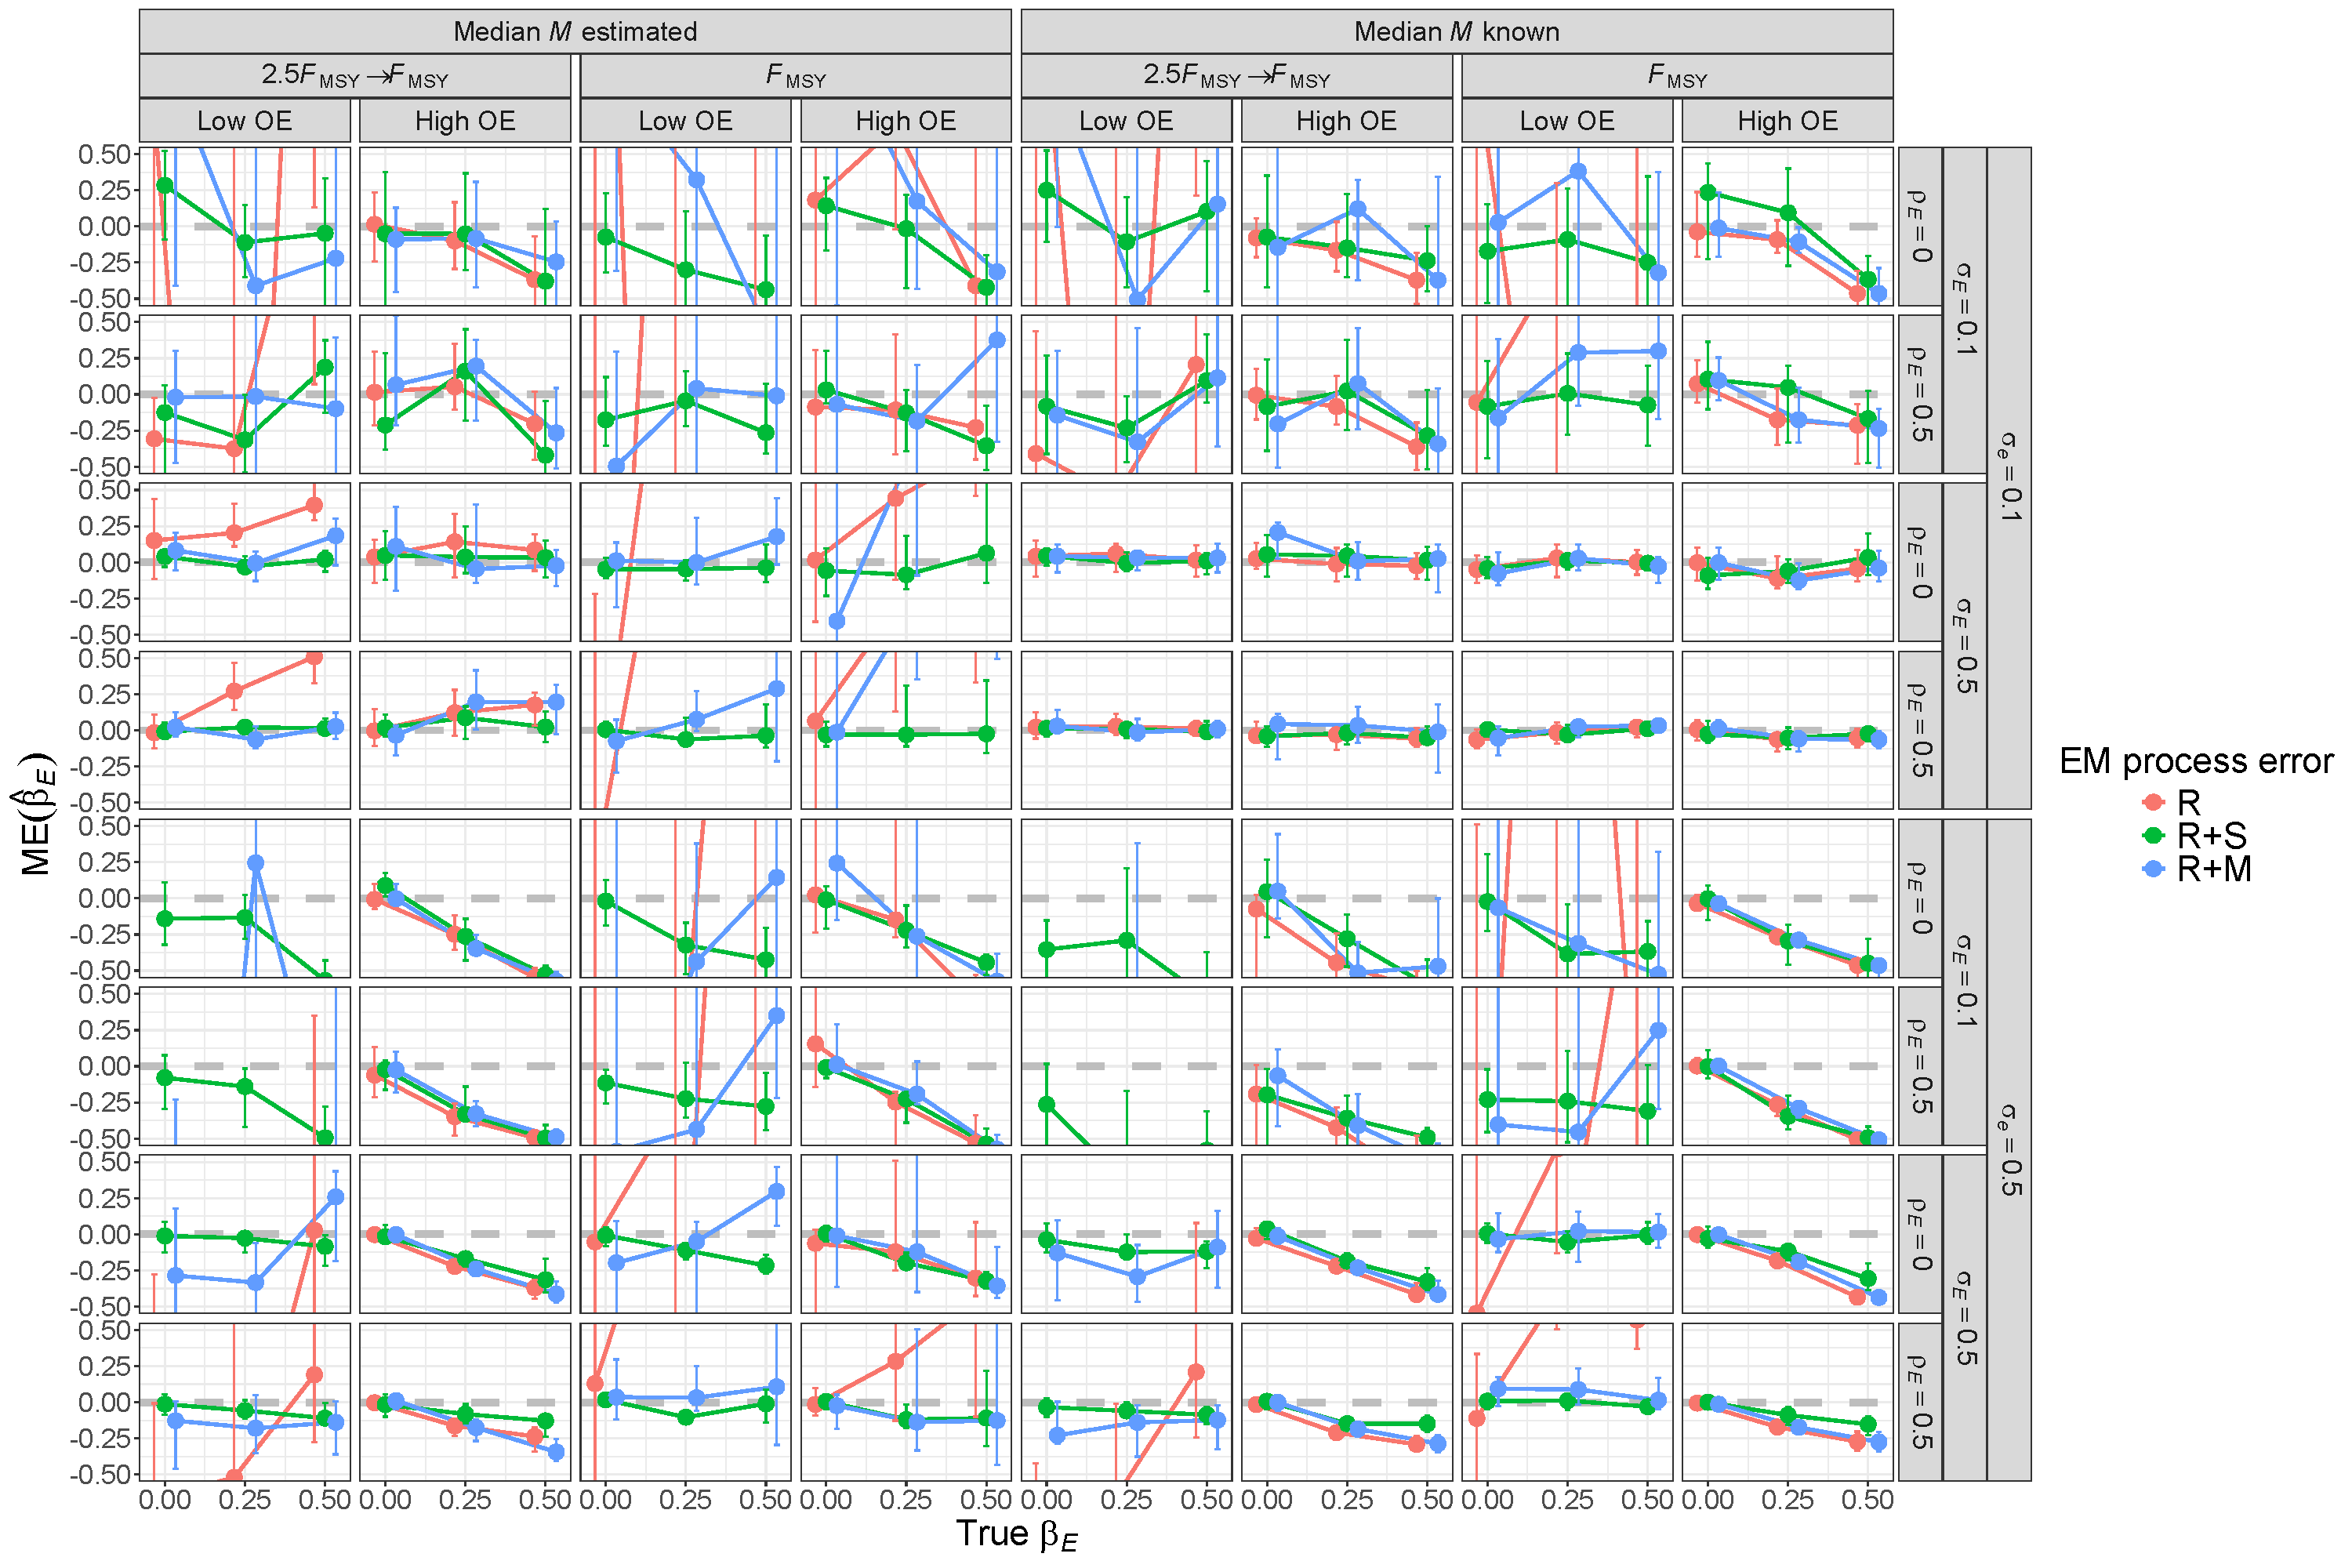
\includegraphics[height = \textheight]{beta_E_bias_RSom}
\end{center}
\caption{\DIFaddFL{For R+S operating models, median error (ME) of estimates of environmental effect on $M$ ($\beta_E$) from fitting estimating models with alternative process error assumptions and treatment of median $M$ parameter ($\beta_M$). Vertical lines represent 95\% confidence intervals.}}\label{beta_E_bias_RSom}
\end{figure}
\end{landscape}

\begin{landscape}
\begin{figure}
\begin{center}
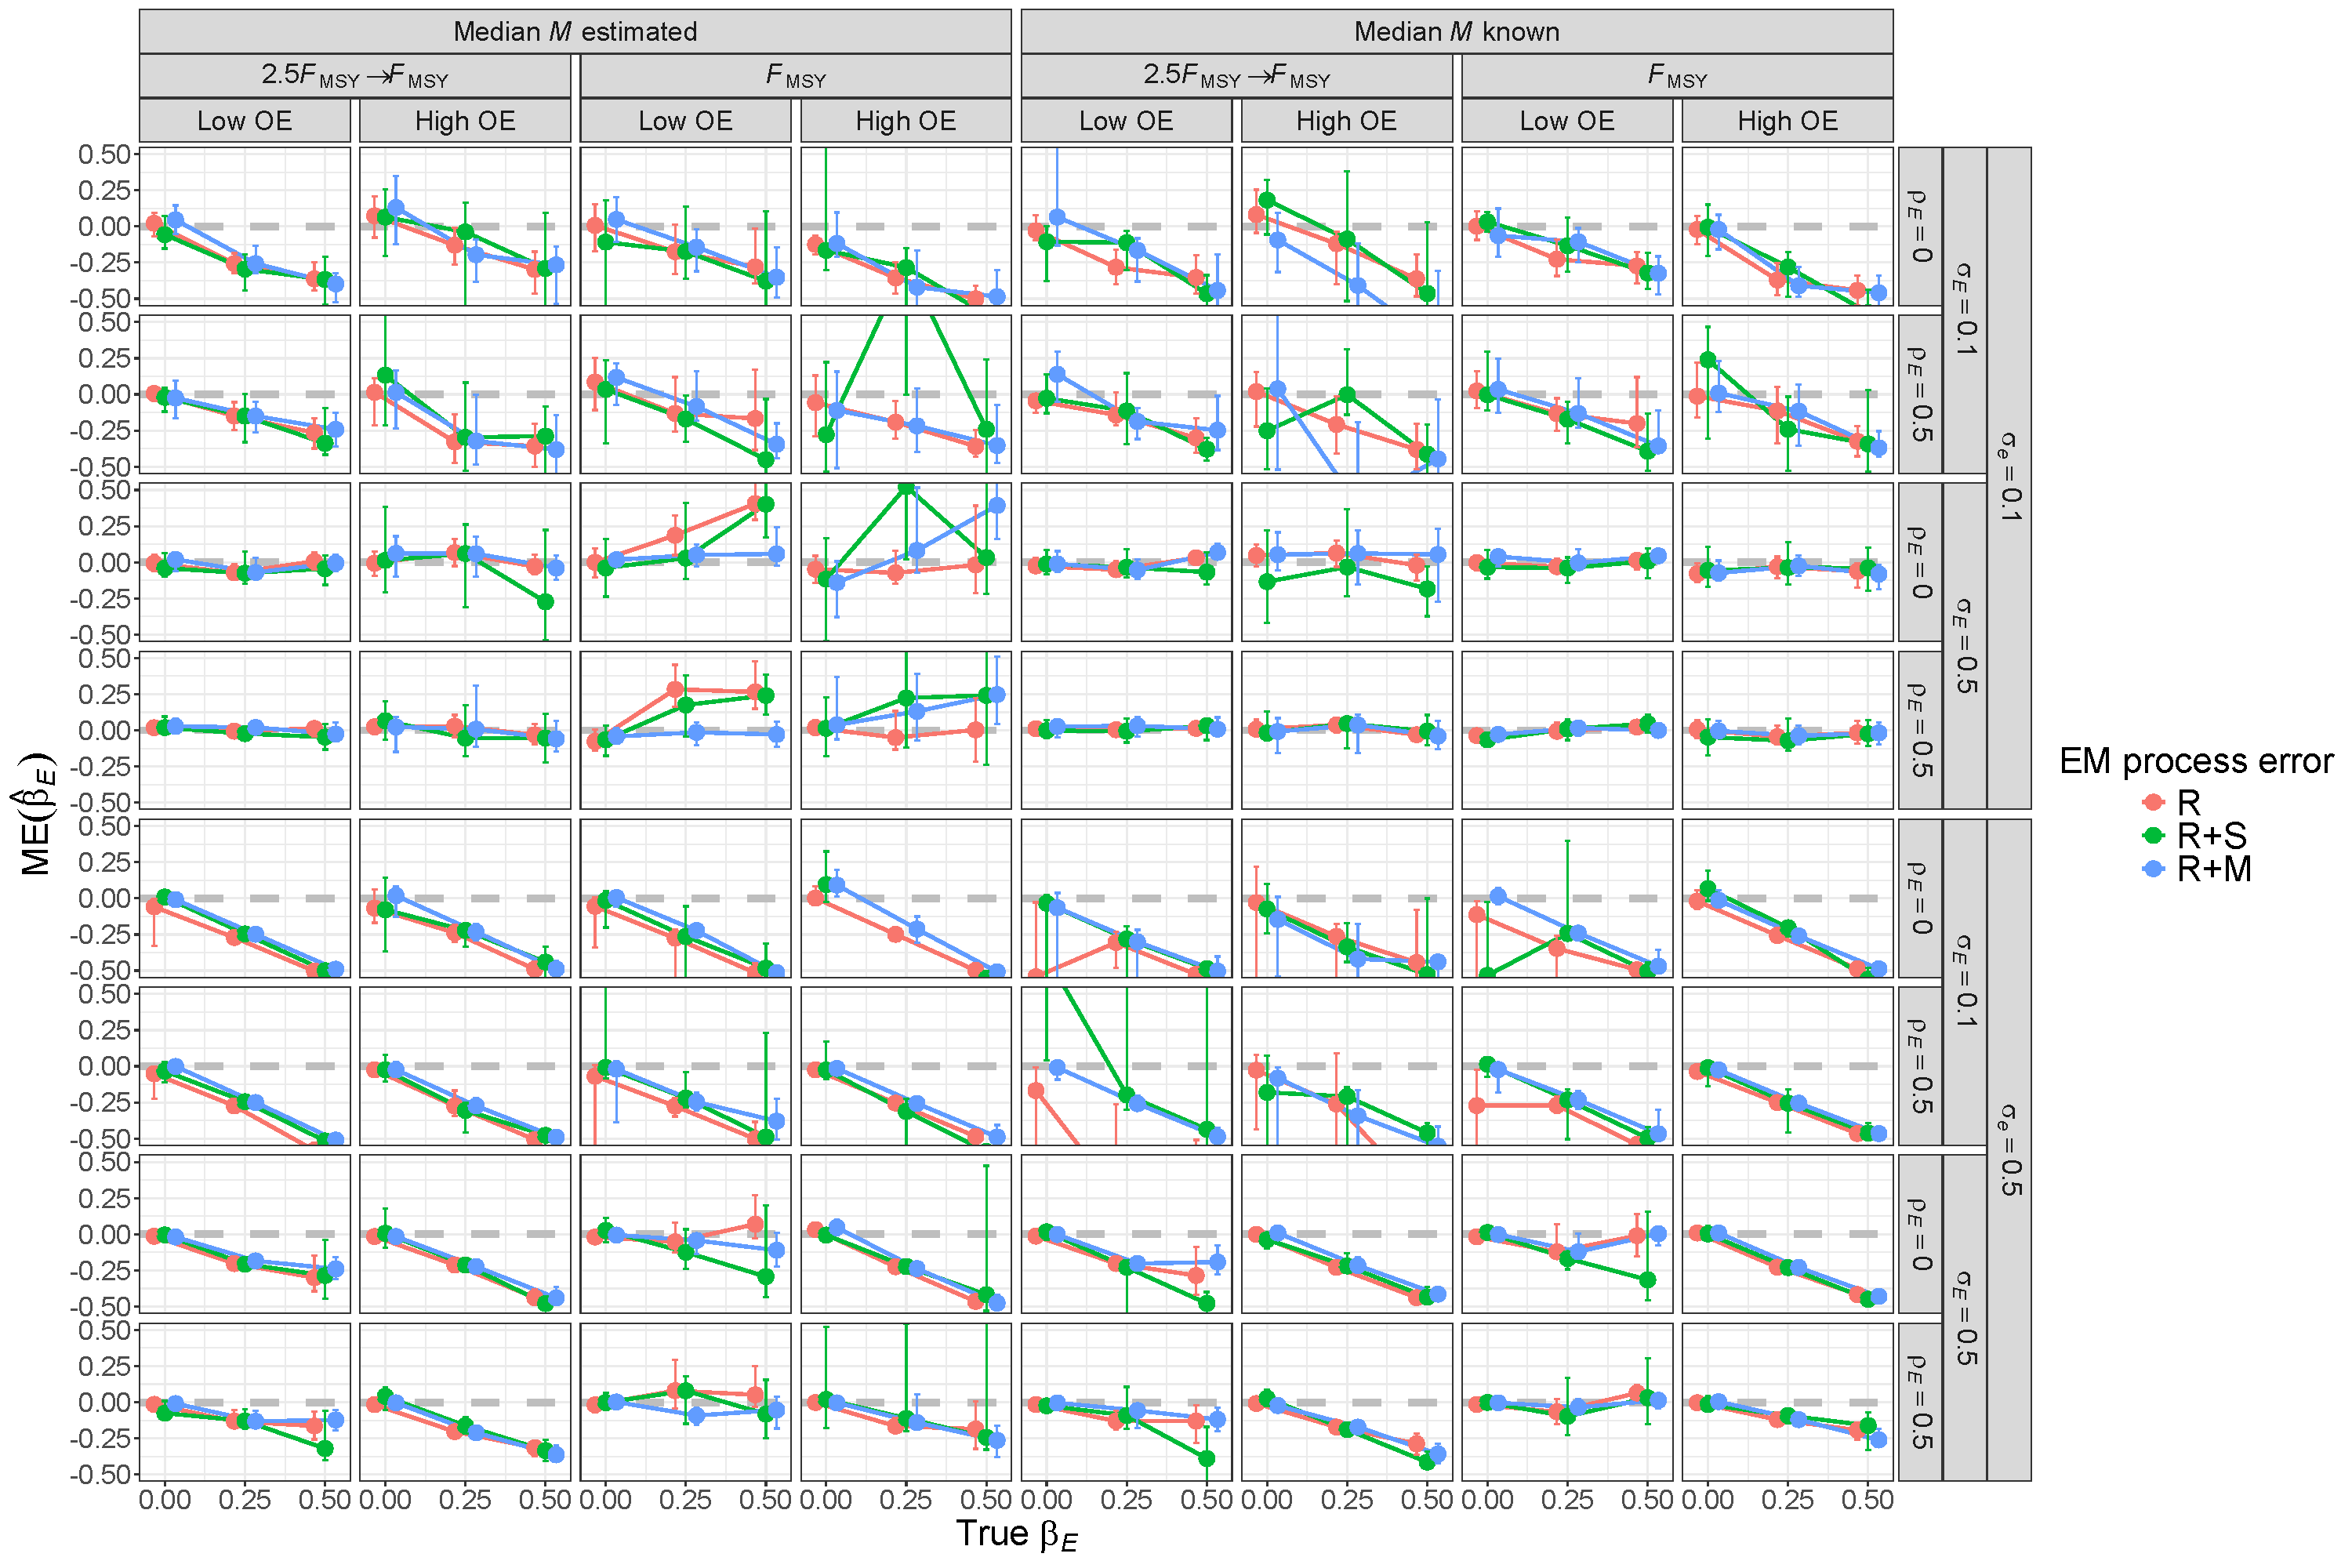
\includegraphics[height = \textheight]{beta_E_bias_RMom}
\end{center}
\caption{\DIFaddFL{For R+M operating models, median error (ME) of estimates of environmental effect on $M$ ($\beta_E$) from fitting estimating models with alternative process error assumptions and treatment of median $M$ parameter ($\beta_M$). Vertical lines represent 95\% confidence intervals.}}\label{beta_E_bias_RMom}
\end{figure}
\end{landscape}

\begin{landscape}
\begin{figure}
\begin{center}
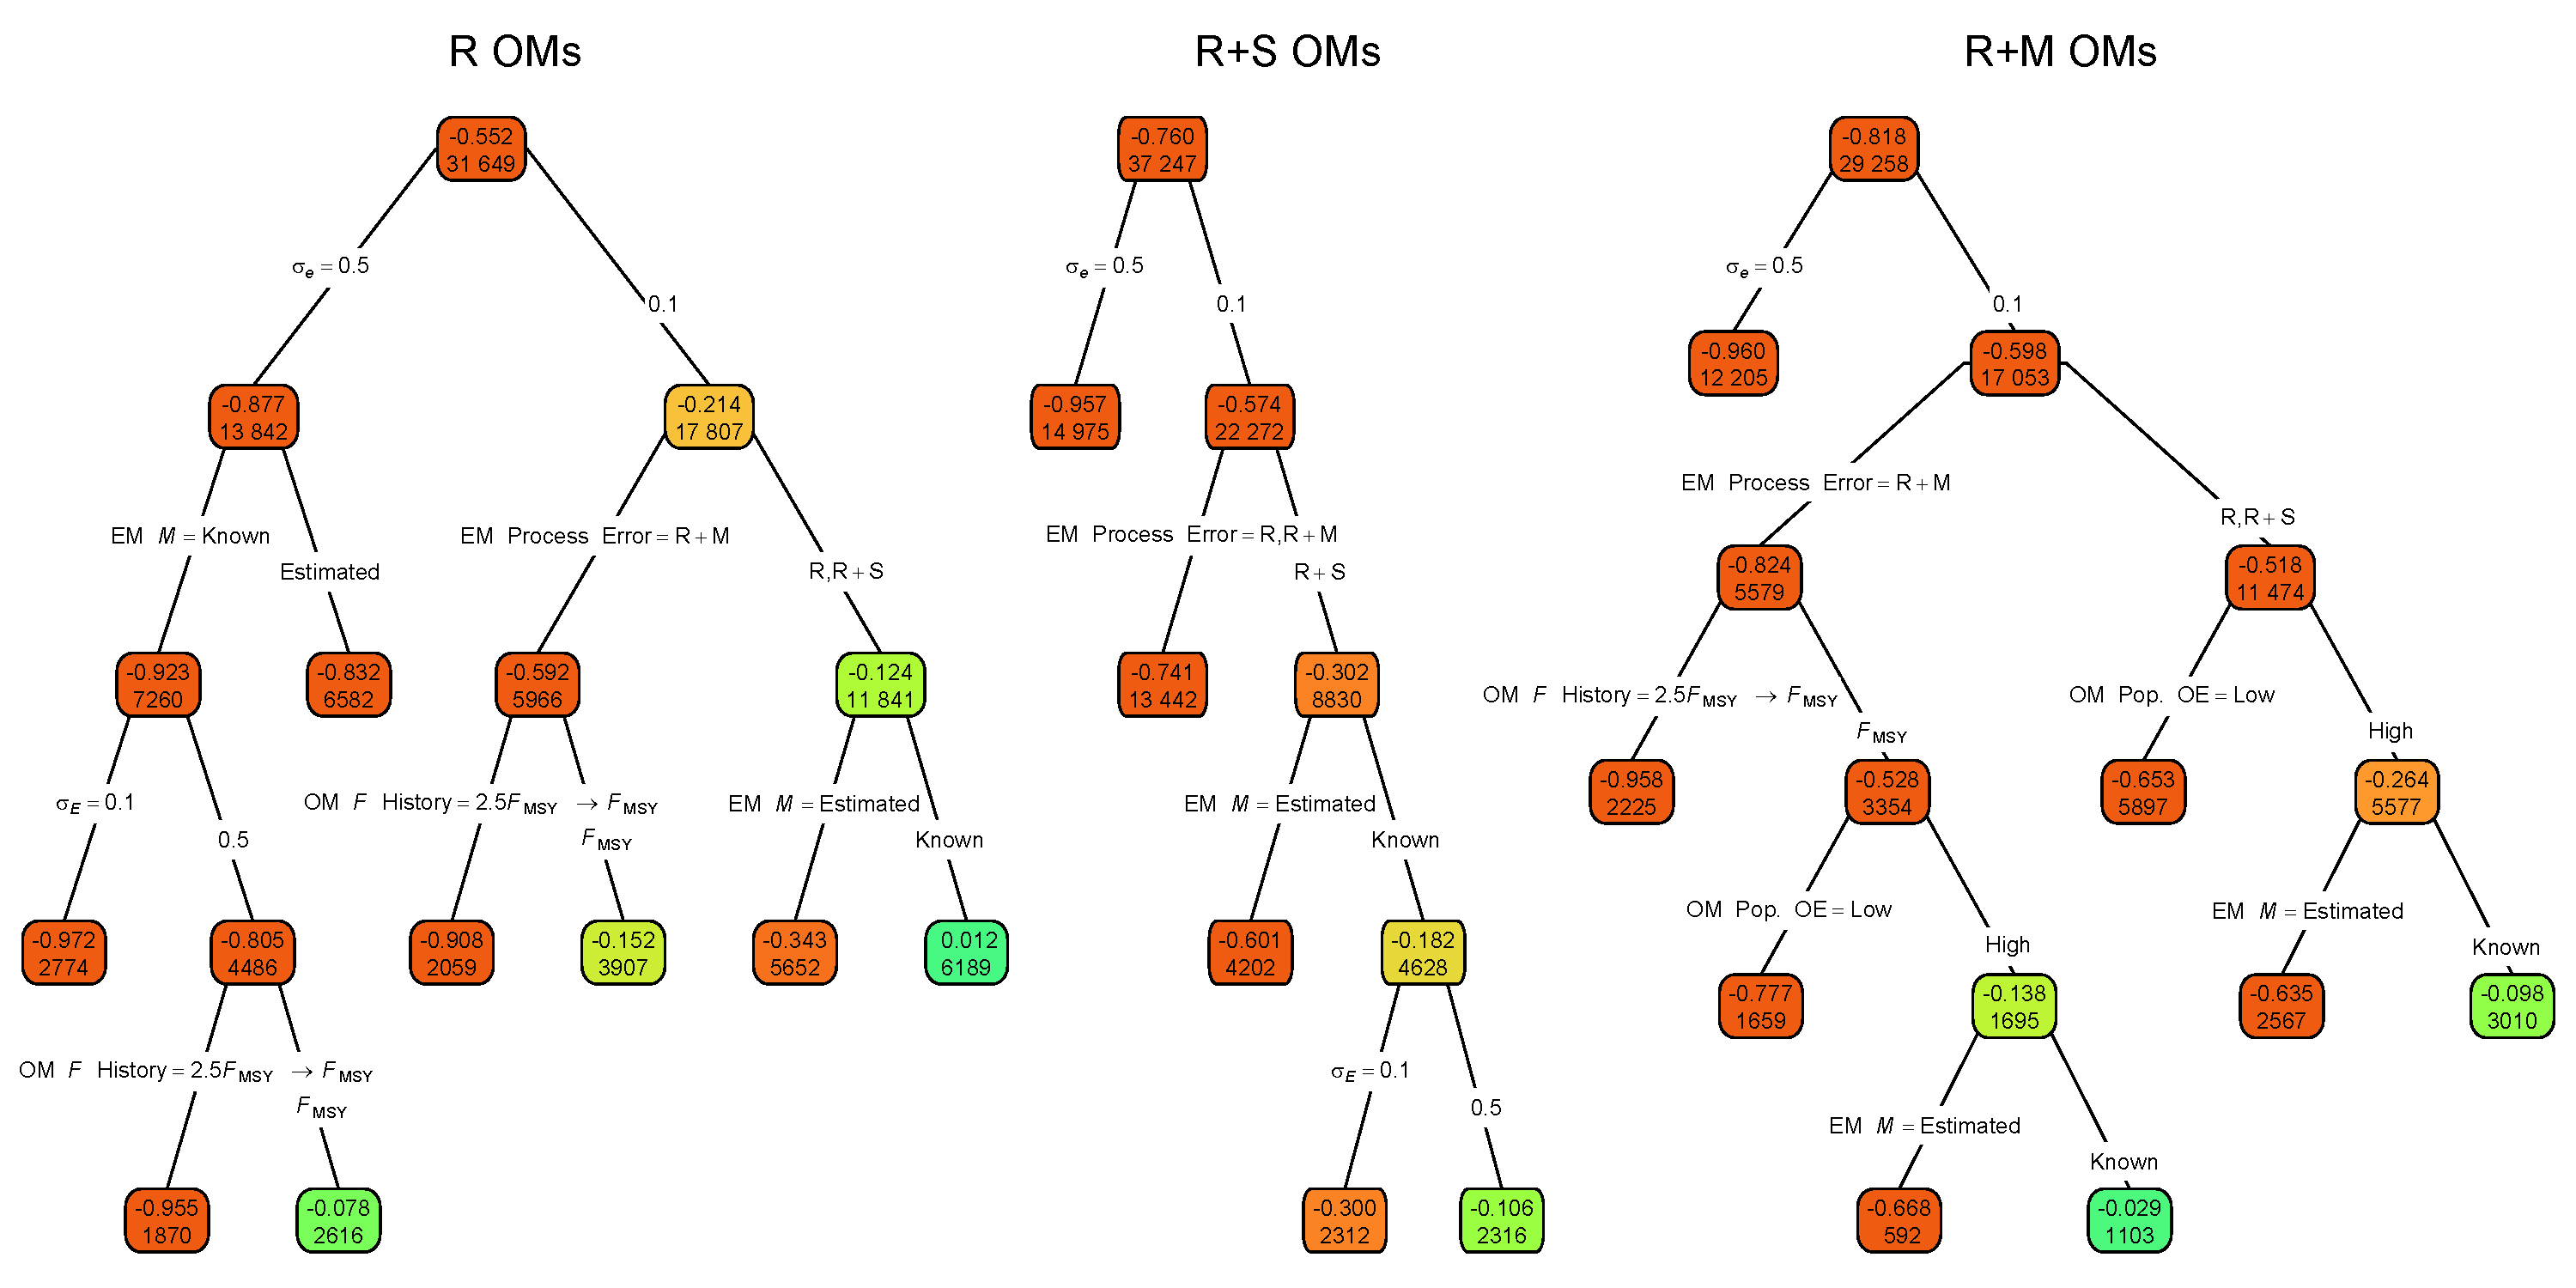
\includegraphics[width = 1.4\textwidth]{ecov_beta_SE_bias_regtree_plots}
\end{center}
\caption{\DIFaddFL{Regression trees for error of the Hessian-based standard error estimates for covariate effect on $M$ ($\widehat {\text{SE}}\left(\widehat \beta_E\right)$). Each node shows the median error for the corresponding subset. Lower or higher absolute median errors are indicated by more green or red polygons, respectively. See Figure \ref{conv_class} caption and Table \ref{factor_table} for further details.}}\label{ecov_effect_SE_bias_regtree}
\end{figure}
\end{landscape}

\begin{landscape}
\begin{figure}
\begin{center}
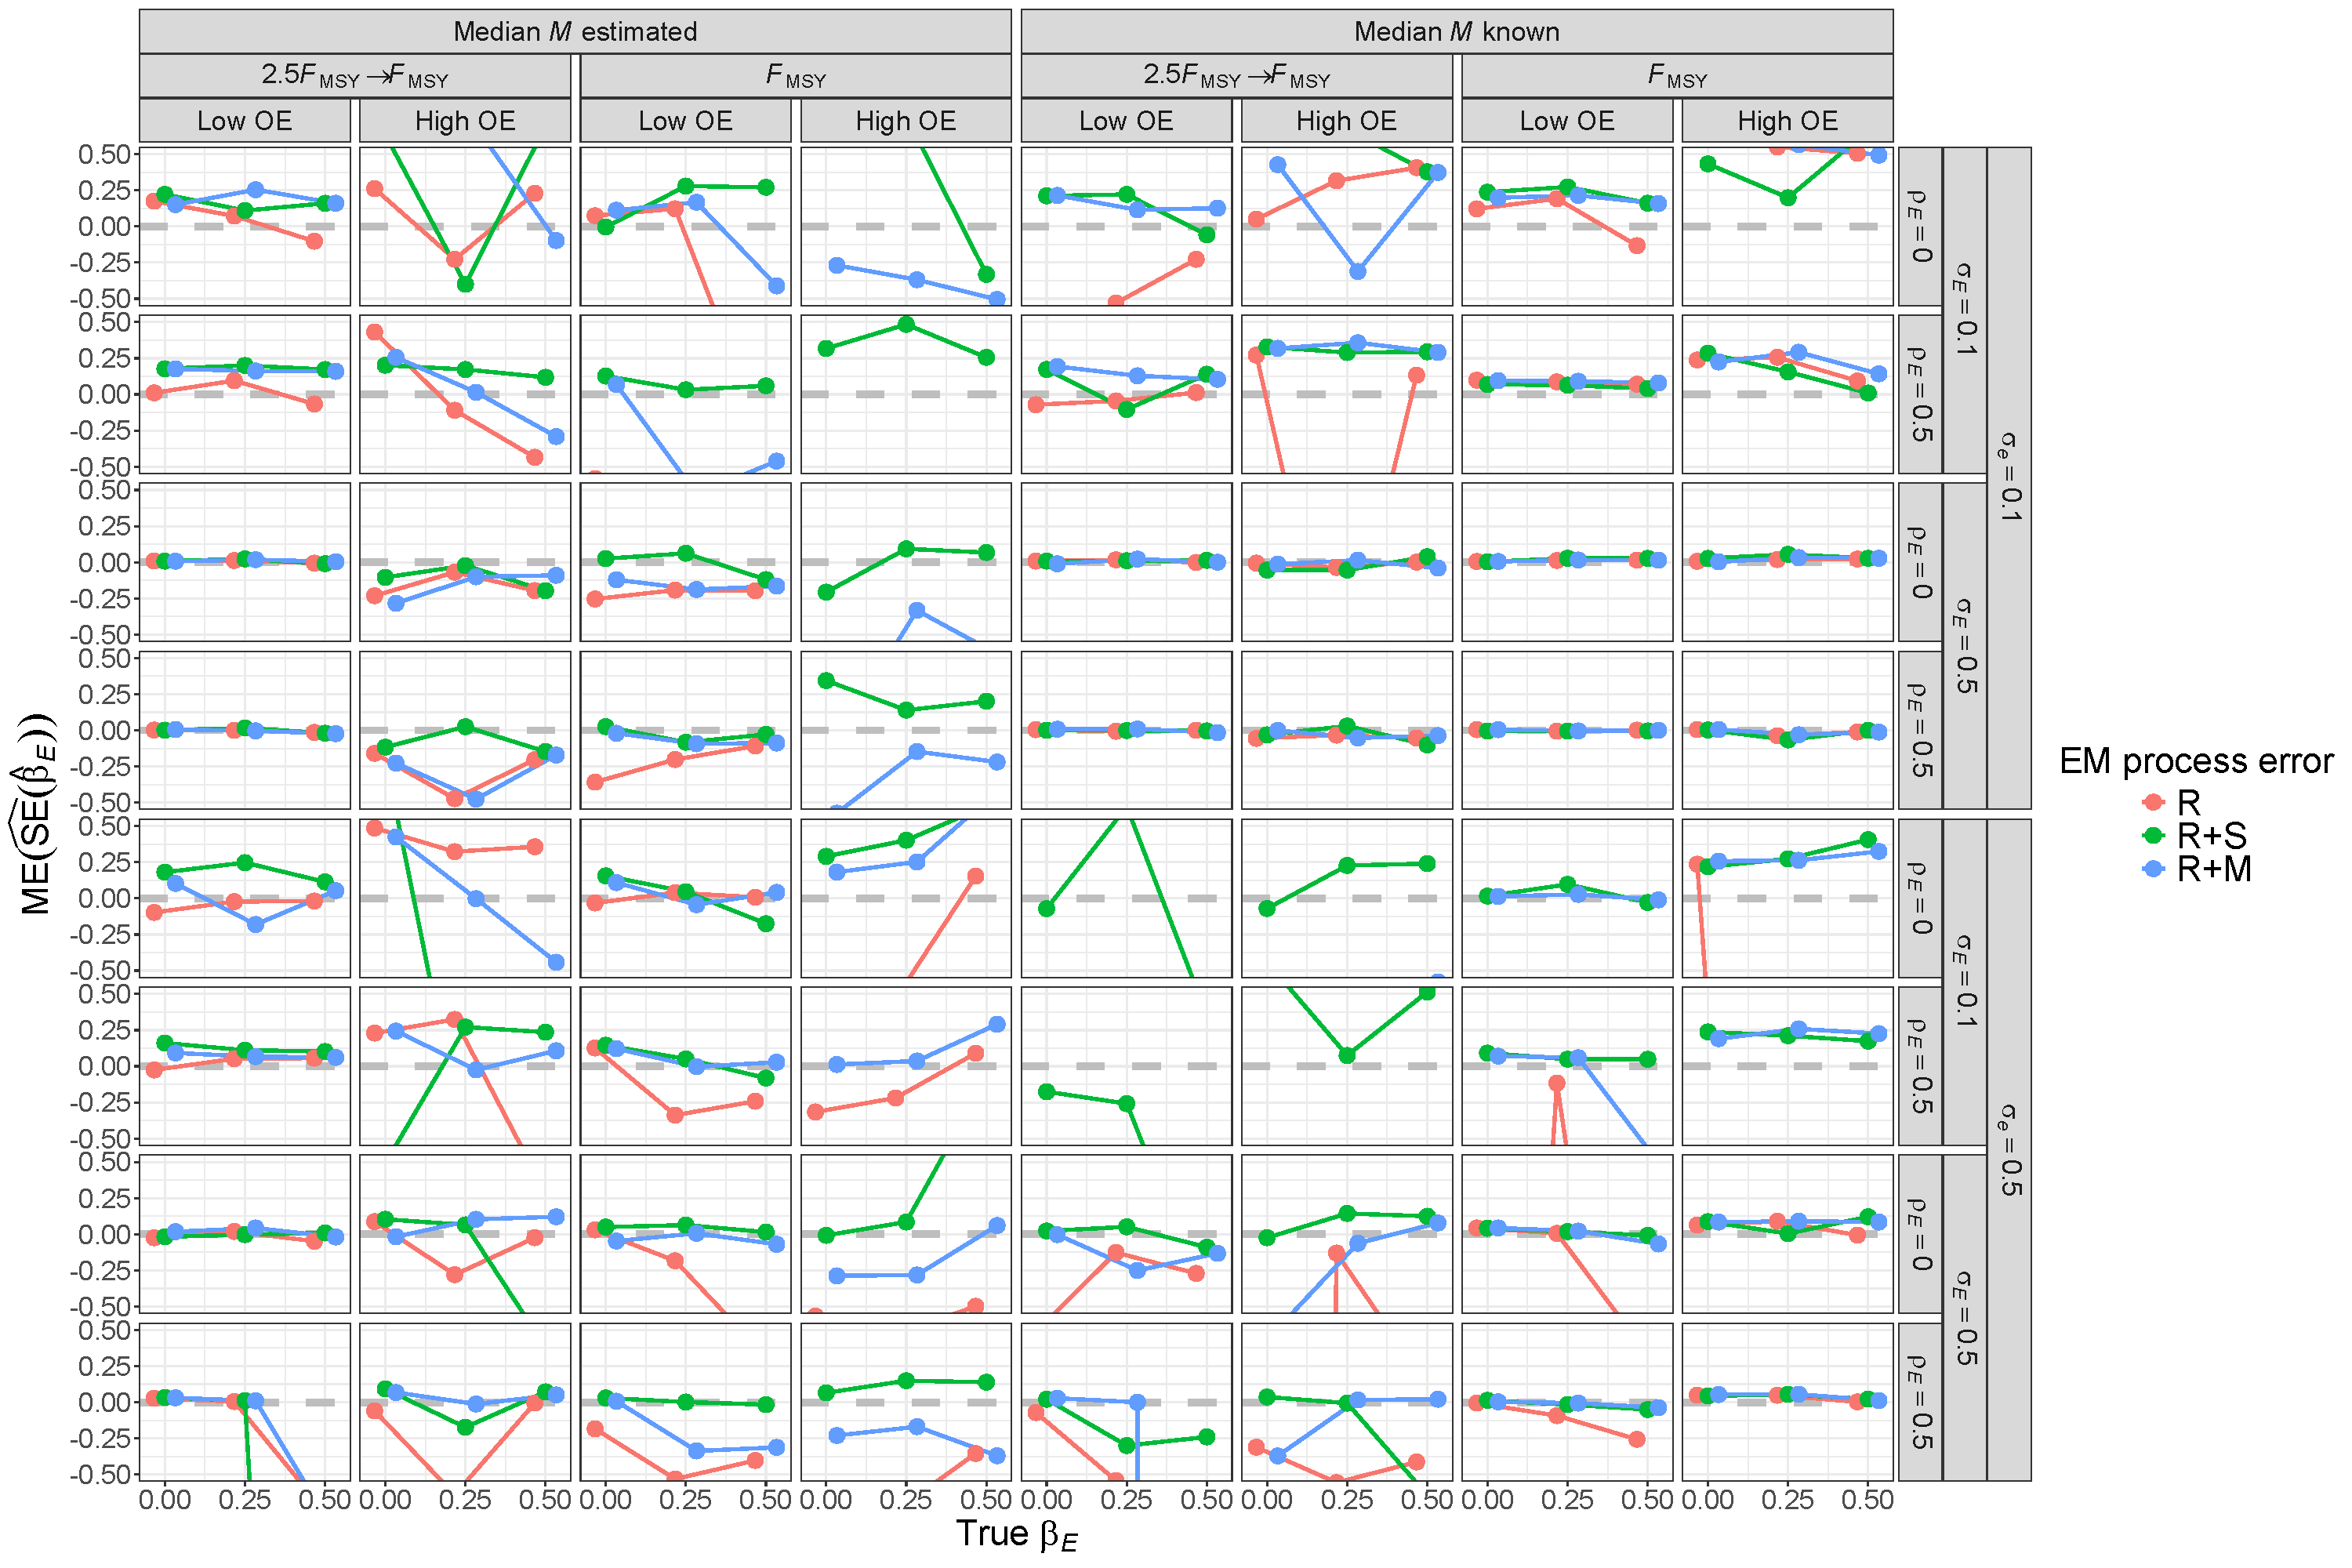
\includegraphics[height = \textheight]{se_beta_E_bias_Rom}
\end{center}
\caption{\DIFaddFL{For R operating models, median error (ME) of Hessian-based estimates of standard error for covariate effect on $M$ ($\beta_E$) from fitting estimating models with alternative process error assumptions and treatment of median $M$ parameter ($\beta_M$). True standard error is defined as the mean of the standard error estimates accross converged fits to simulated data sets for a given operating model scenario.}}\label{se_beta_E_bias_Rom}
\end{figure}
\end{landscape}

\begin{landscape}
\begin{figure}
\begin{center}
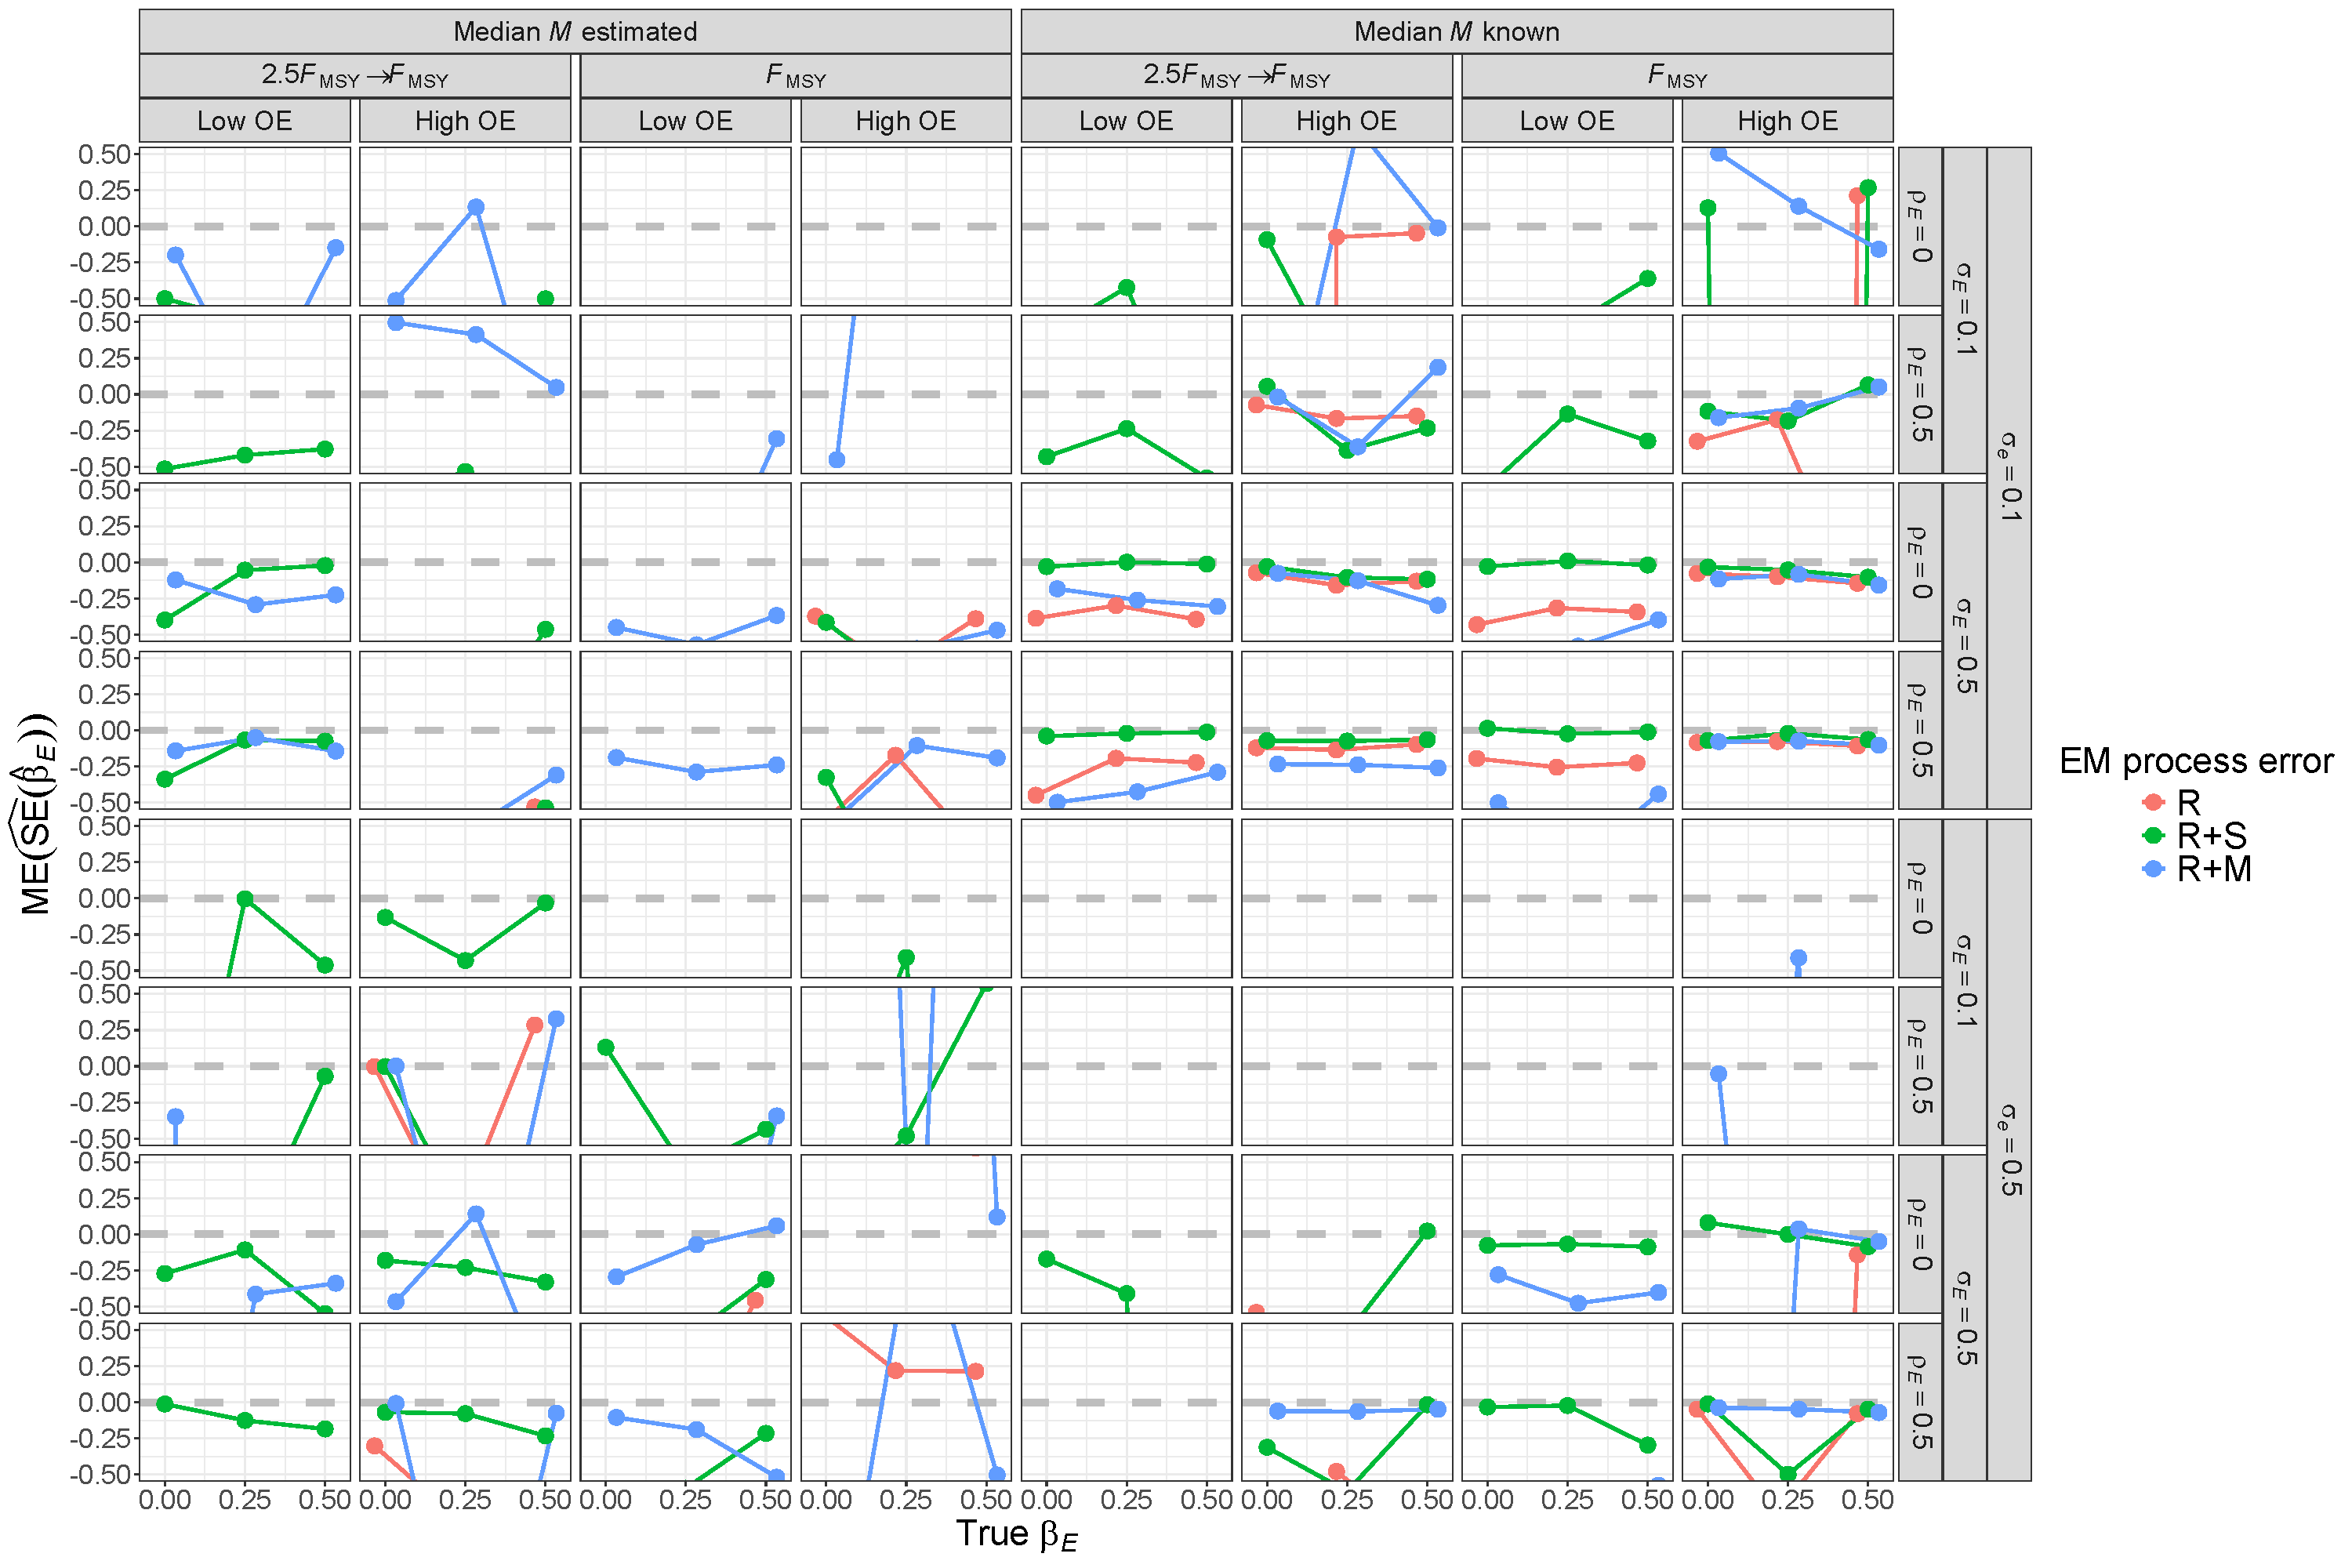
\includegraphics[height = \textheight]{se_beta_E_bias_RSom}
\end{center}
\caption{\DIFaddFL{For R+S operating models, median error (ME) of Hessian-based estimates of standard error for covariate effect on $M$ ($\beta_E$) from fitting estimating models with alternative process error assumptions and treatment of median $M$ parameter ($\beta_M$). True standard error is defined as the mean of the standard error estimates accross converged fits to simulated data sets for a given operating model scenario.}}\label{se_beta_E_bias_RSom}
\end{figure}
\end{landscape}

\begin{landscape}
\begin{figure}
\begin{center}
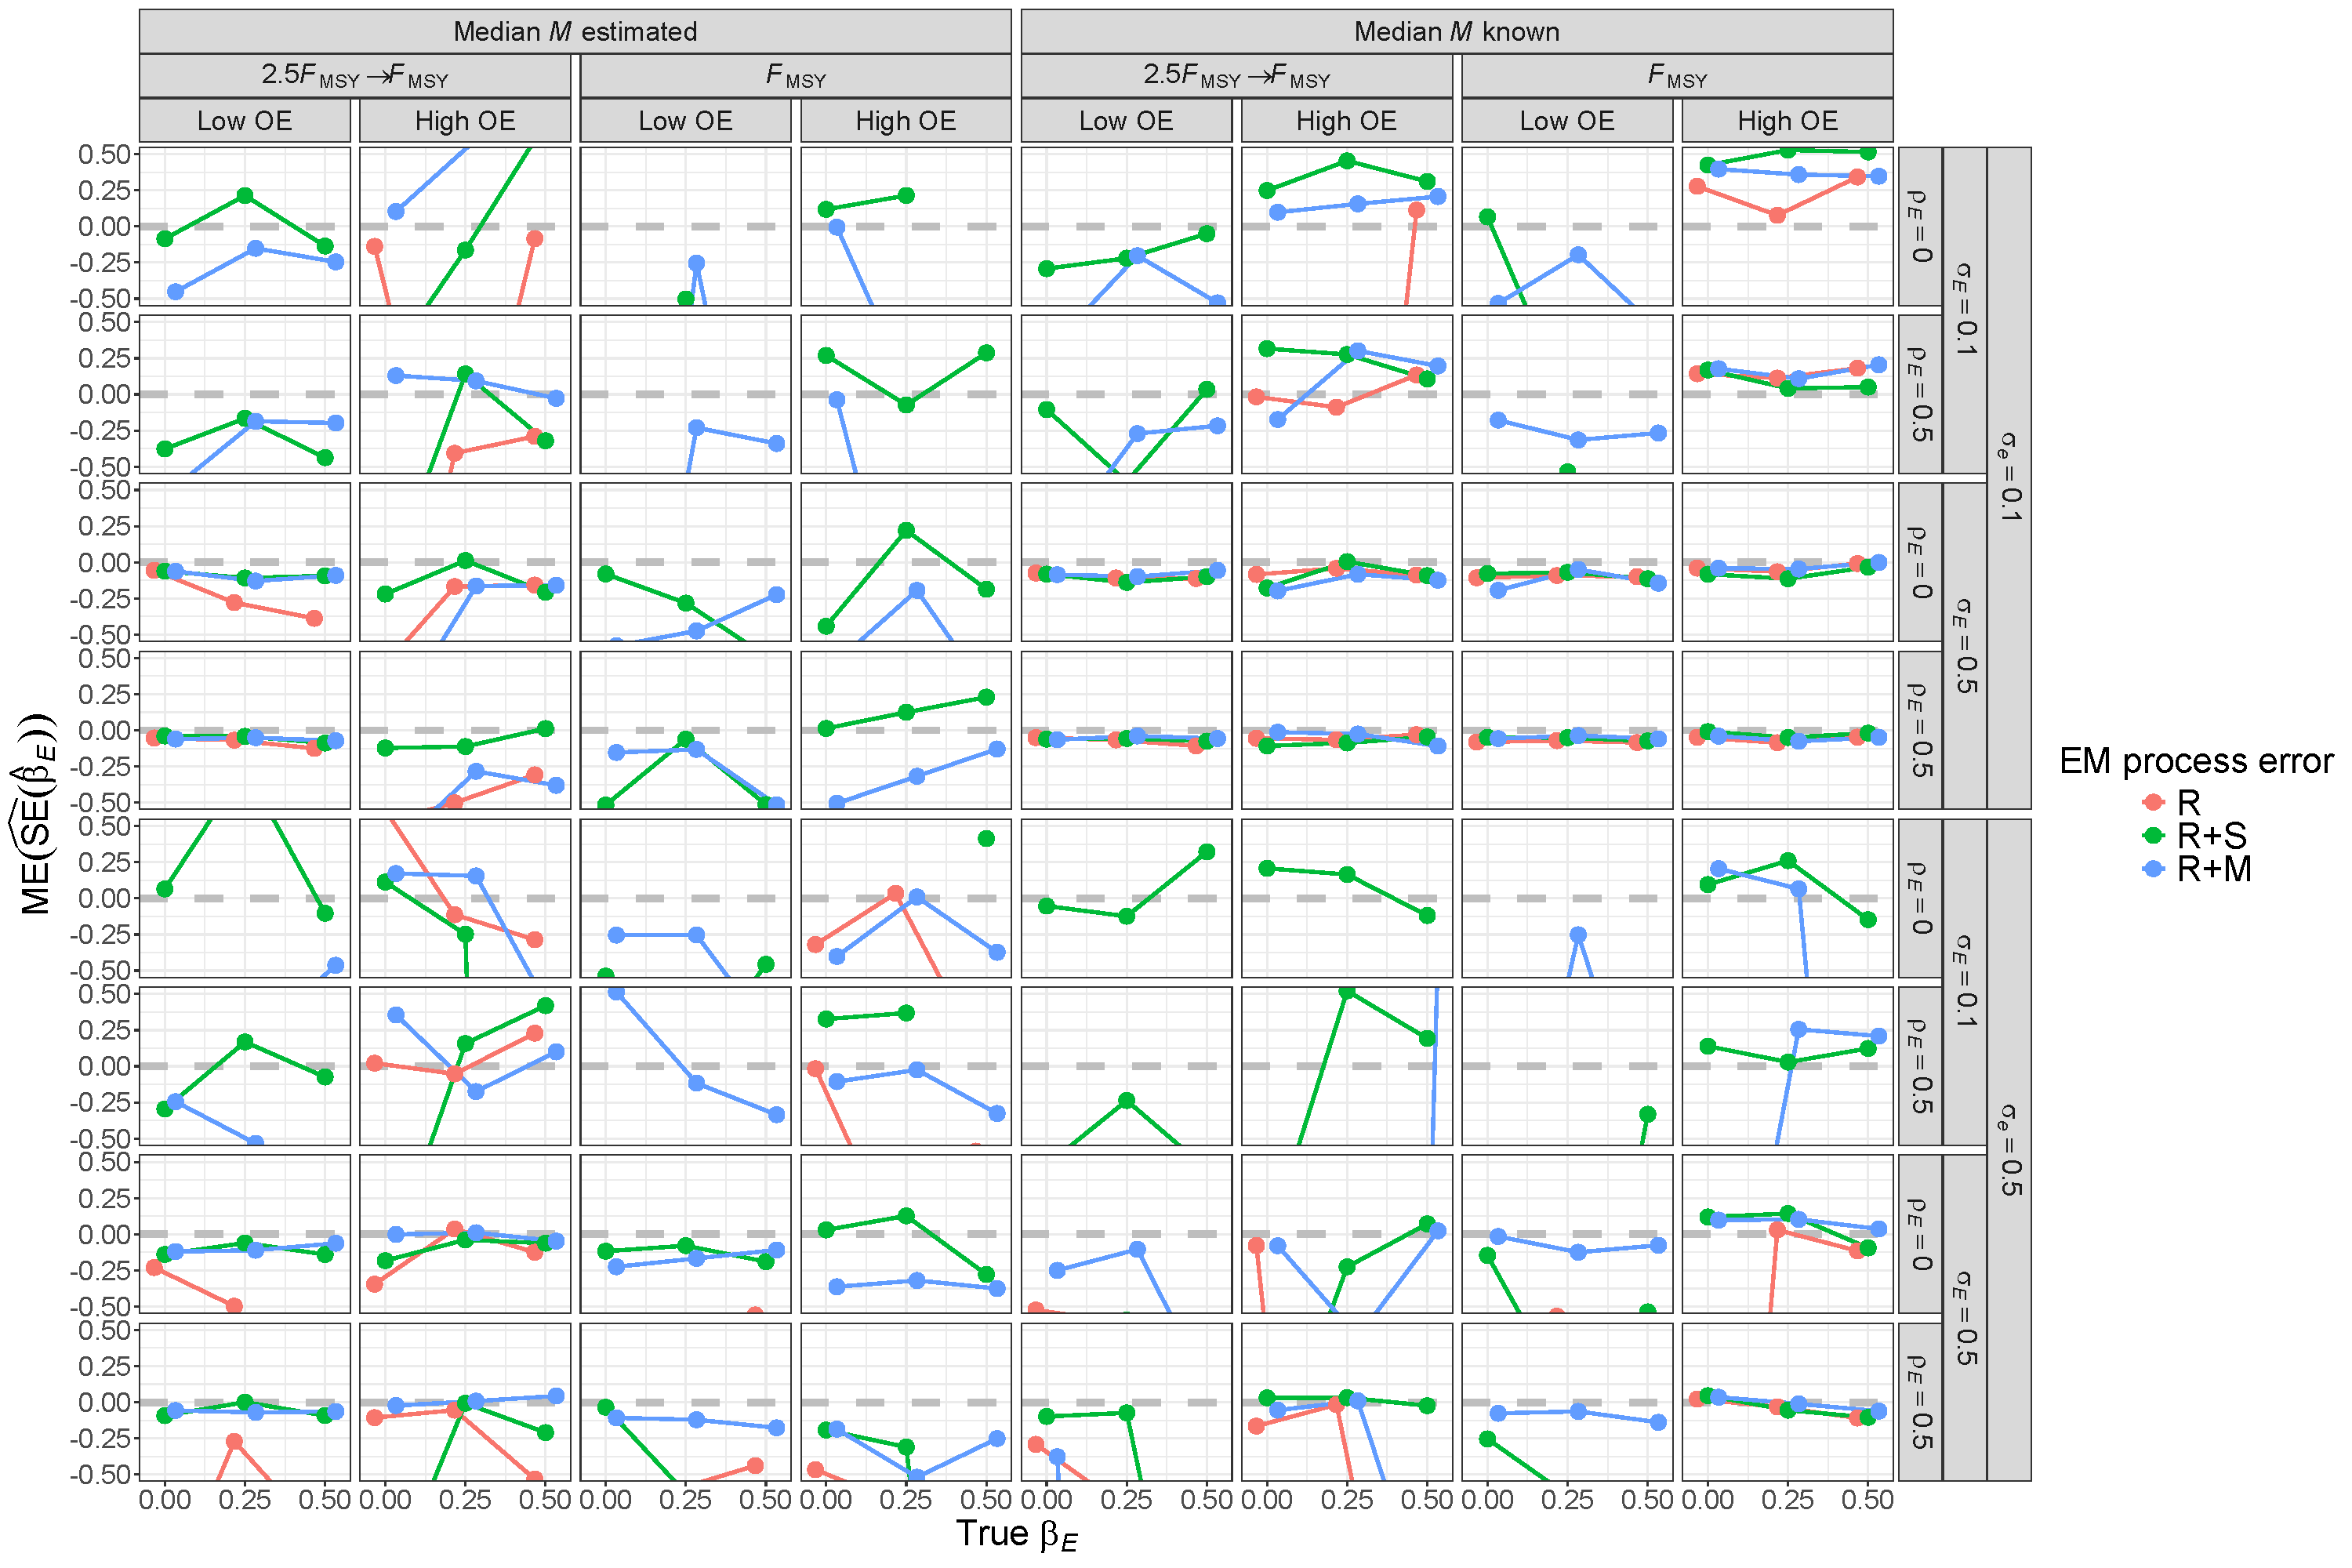
\includegraphics[height = \textheight]{se_beta_E_bias_RMom}
\end{center}
\caption{\DIFaddFL{For R+M operating models, median error (ME) of Hessian-based estimates of standard error for covariate effect on $M$ ($\beta_E$) from fitting estimating models with alternative process error assumptions and treatment of median $M$ parameter ($\beta_M$). True standard error is defined as the mean of the standard error estimates accross converged fits to simulated data sets for a given operating model scenario.}}\label{se_beta_E_bias_RMom}
\end{figure}
\end{landscape}

\begin{landscape}
\begin{figure}
\begin{center}
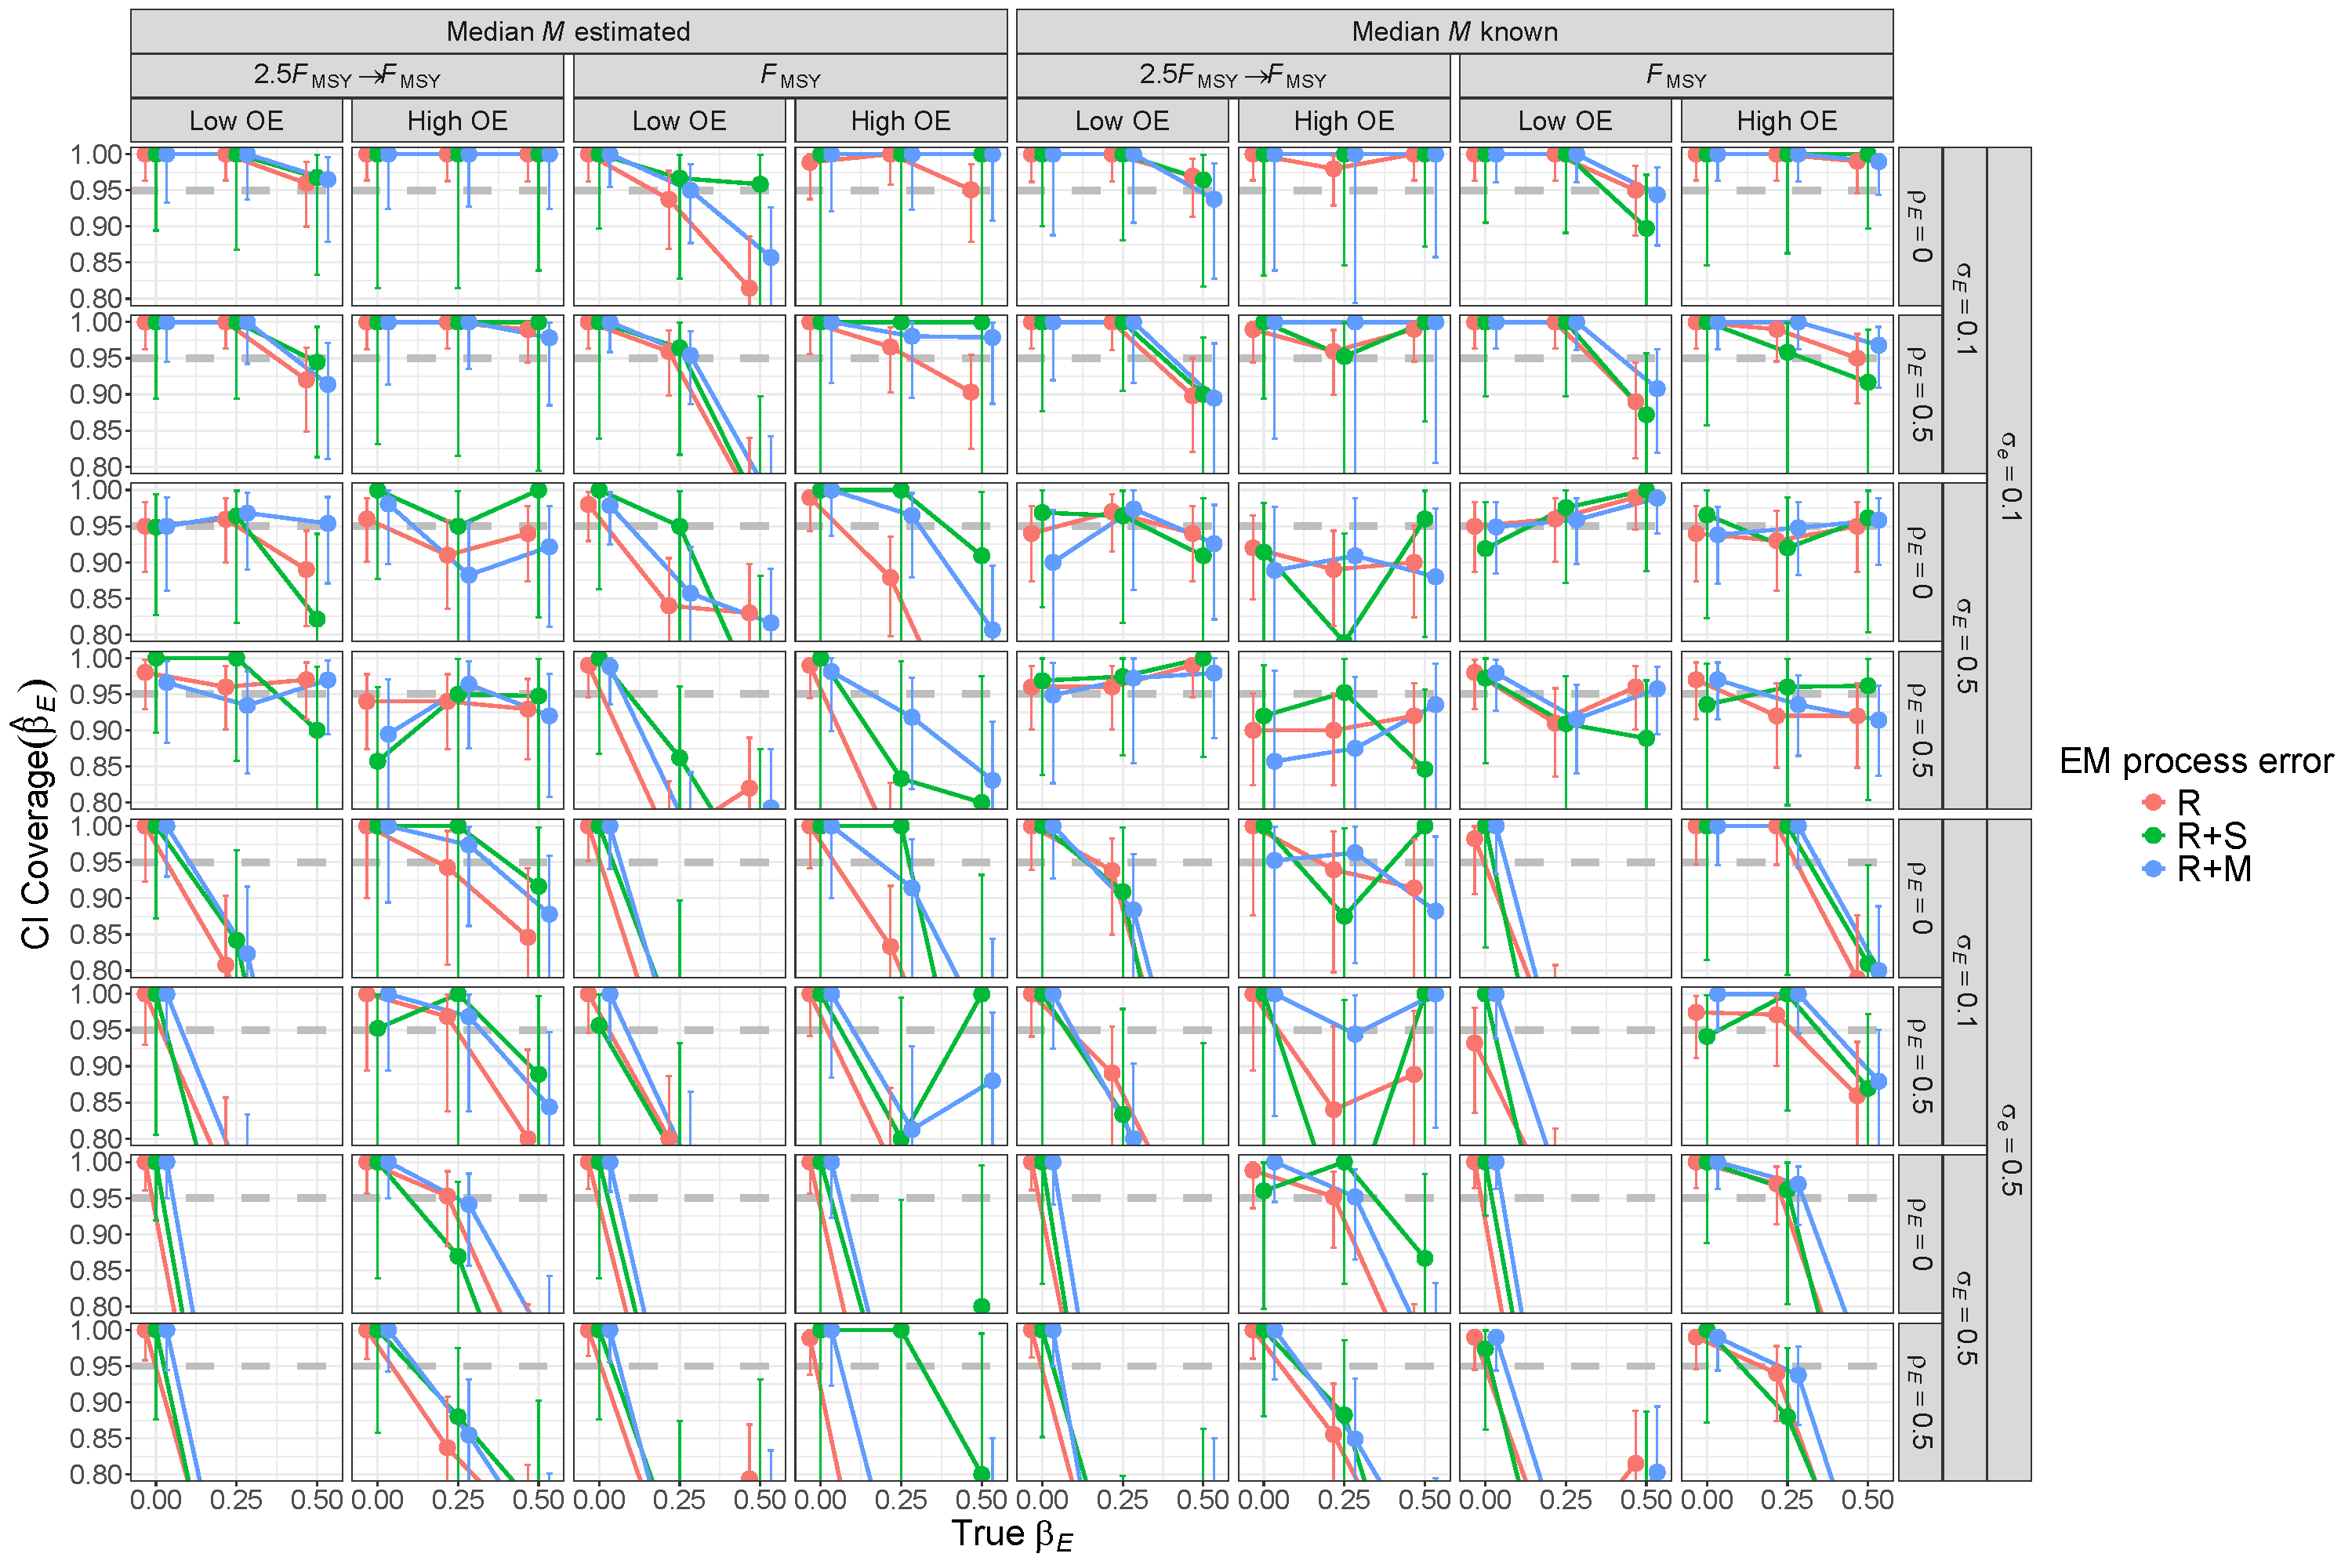
\includegraphics[height = \textheight]{beta_E_CI_coverage_Rom}
\end{center}
\caption{\DIFaddFL{For R operating models, probability of 95\% confidence interval for $\beta_E$ containing the true value for estimating models with alternative process error assumptions and treatment of median $M$ parameter ($\beta_M$). Vertical lines represent 95\% confidence intervals.}}\label{beta_E_CI_coverage_Rom}
\end{figure}
\end{landscape}

\begin{landscape}
\begin{figure}
\begin{center}
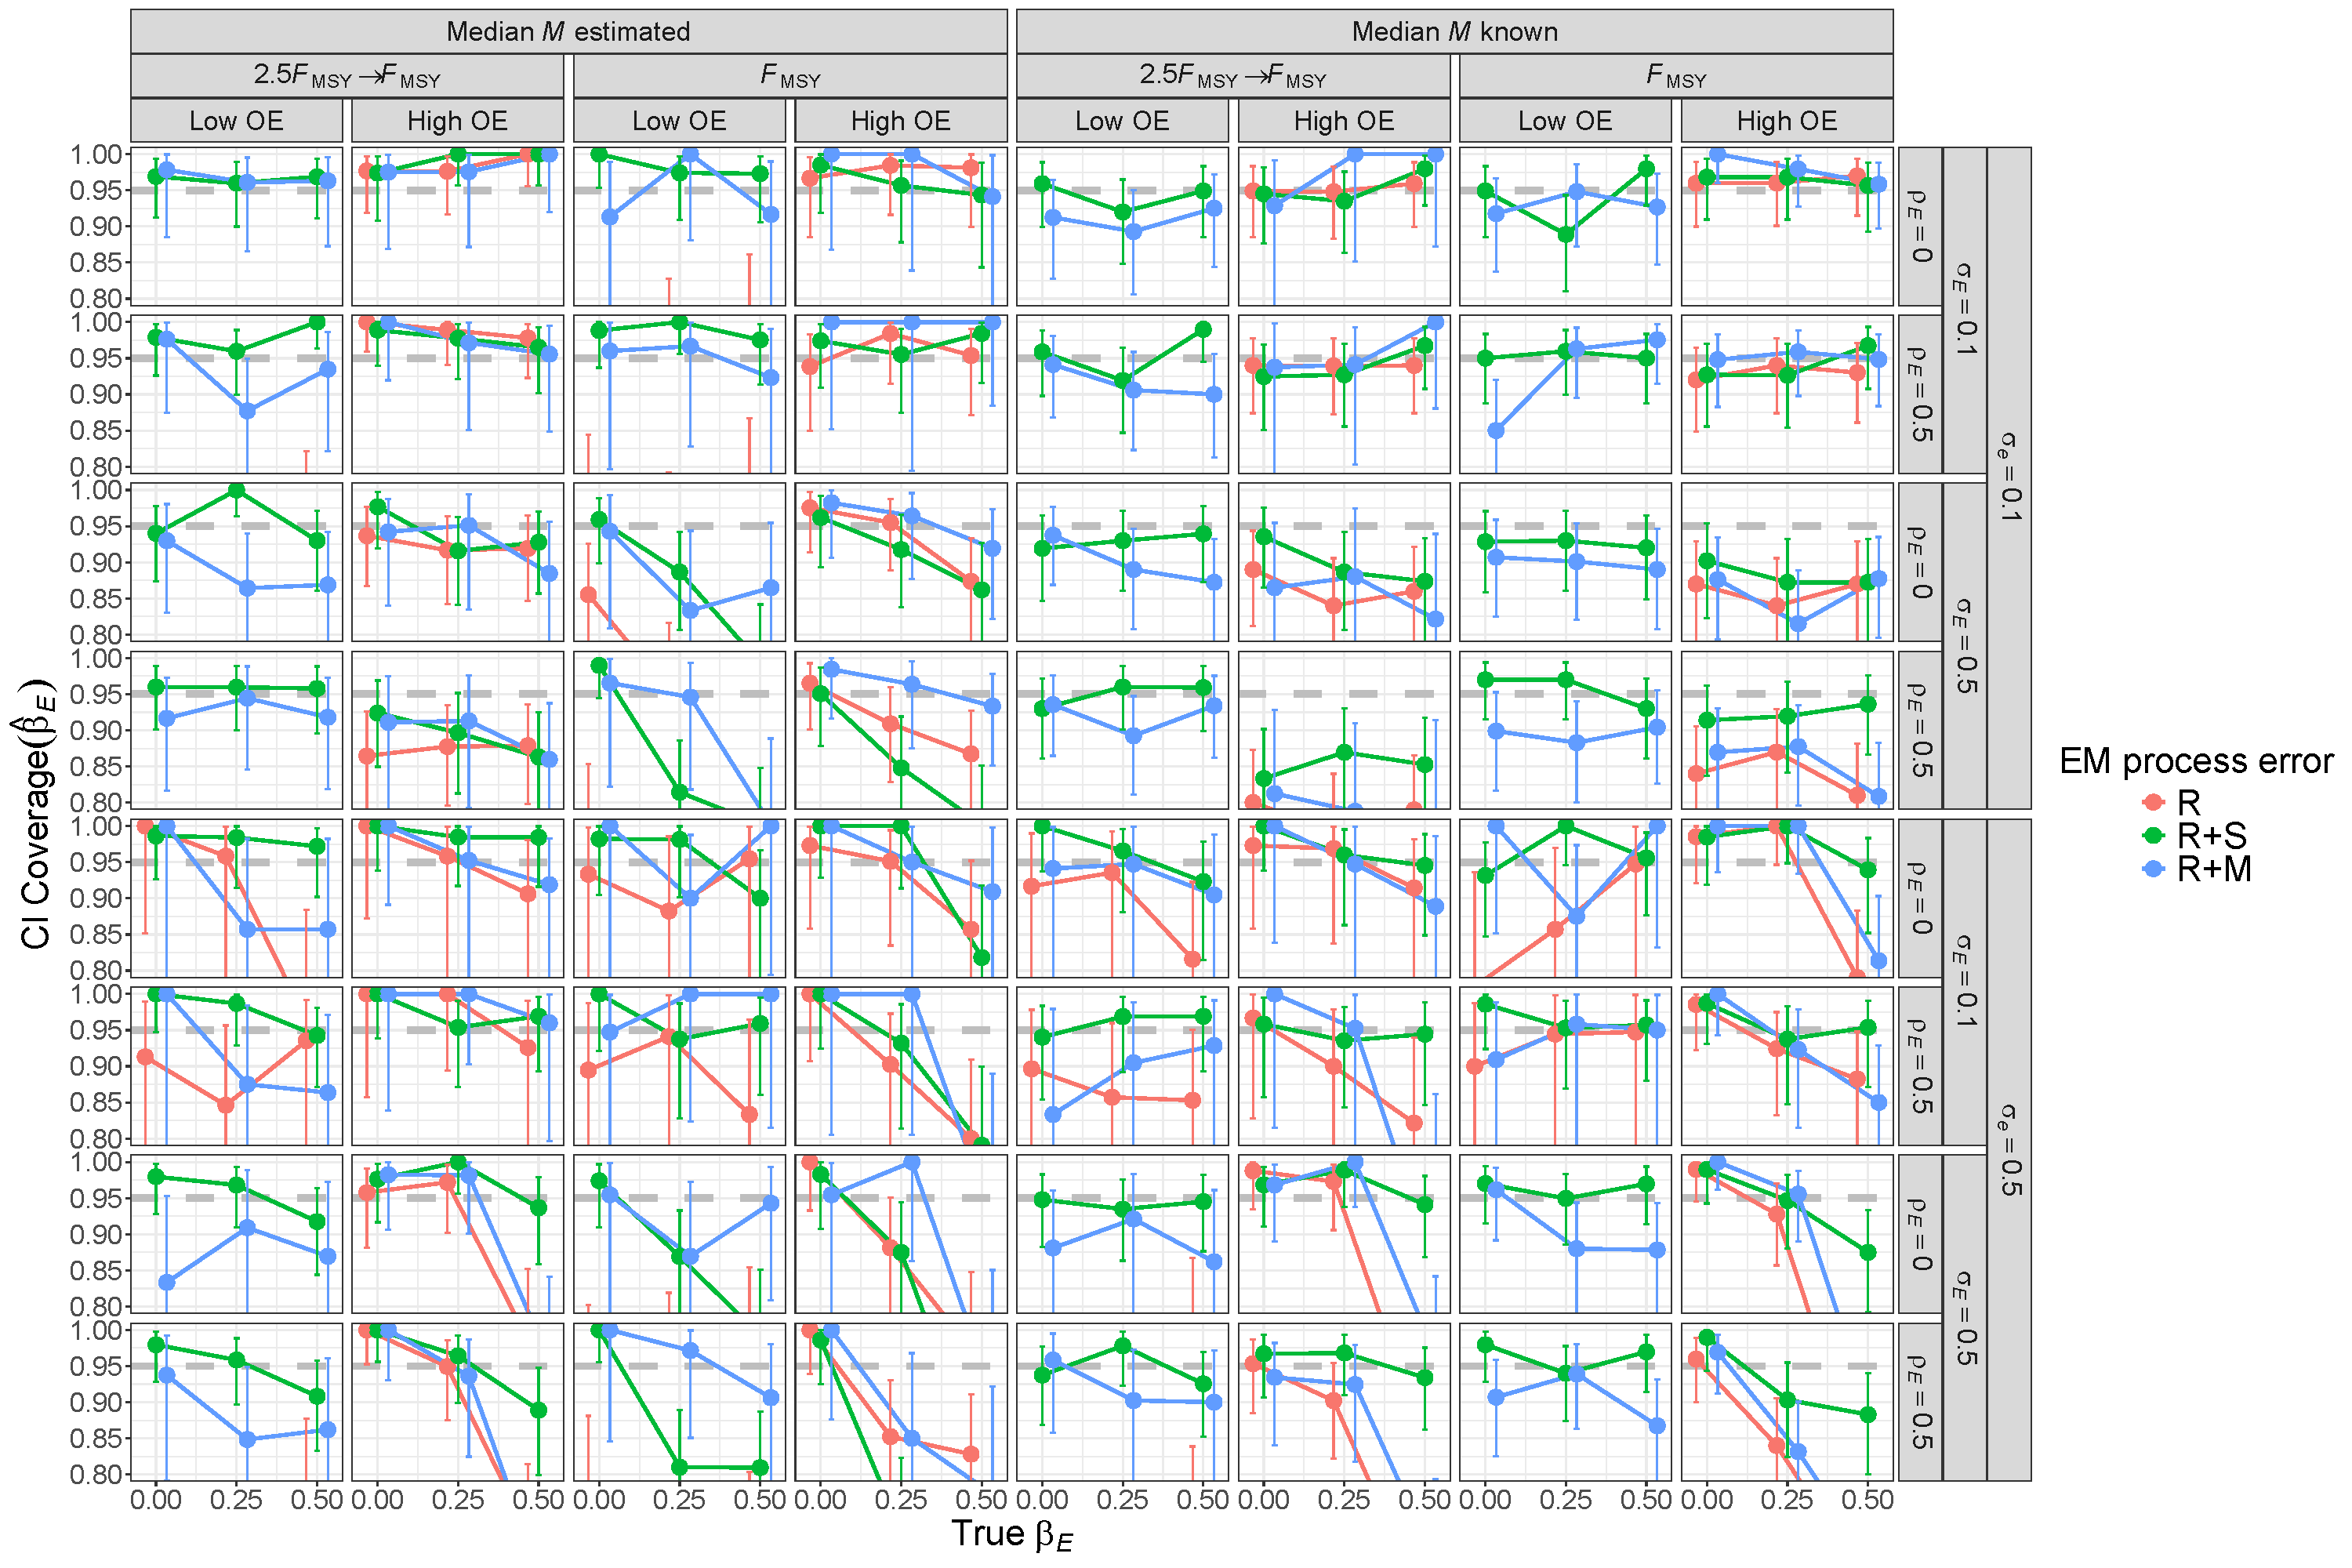
\includegraphics[height = \textheight]{beta_E_CI_coverage_RSom}
\end{center}
\caption{\DIFaddFL{For R+S operating models, probability of 95\% confidence interval for $\beta_E$ containing the true value for estimating models with alternative process error assumptions and treatment of median $M$ parameter ($\beta_M$). Vertical lines represent 95\% confidence intervals.}}\label{beta_E_CI_coverage_RSom}
\end{figure}
\end{landscape}

\begin{landscape}
\begin{figure}
\begin{center}
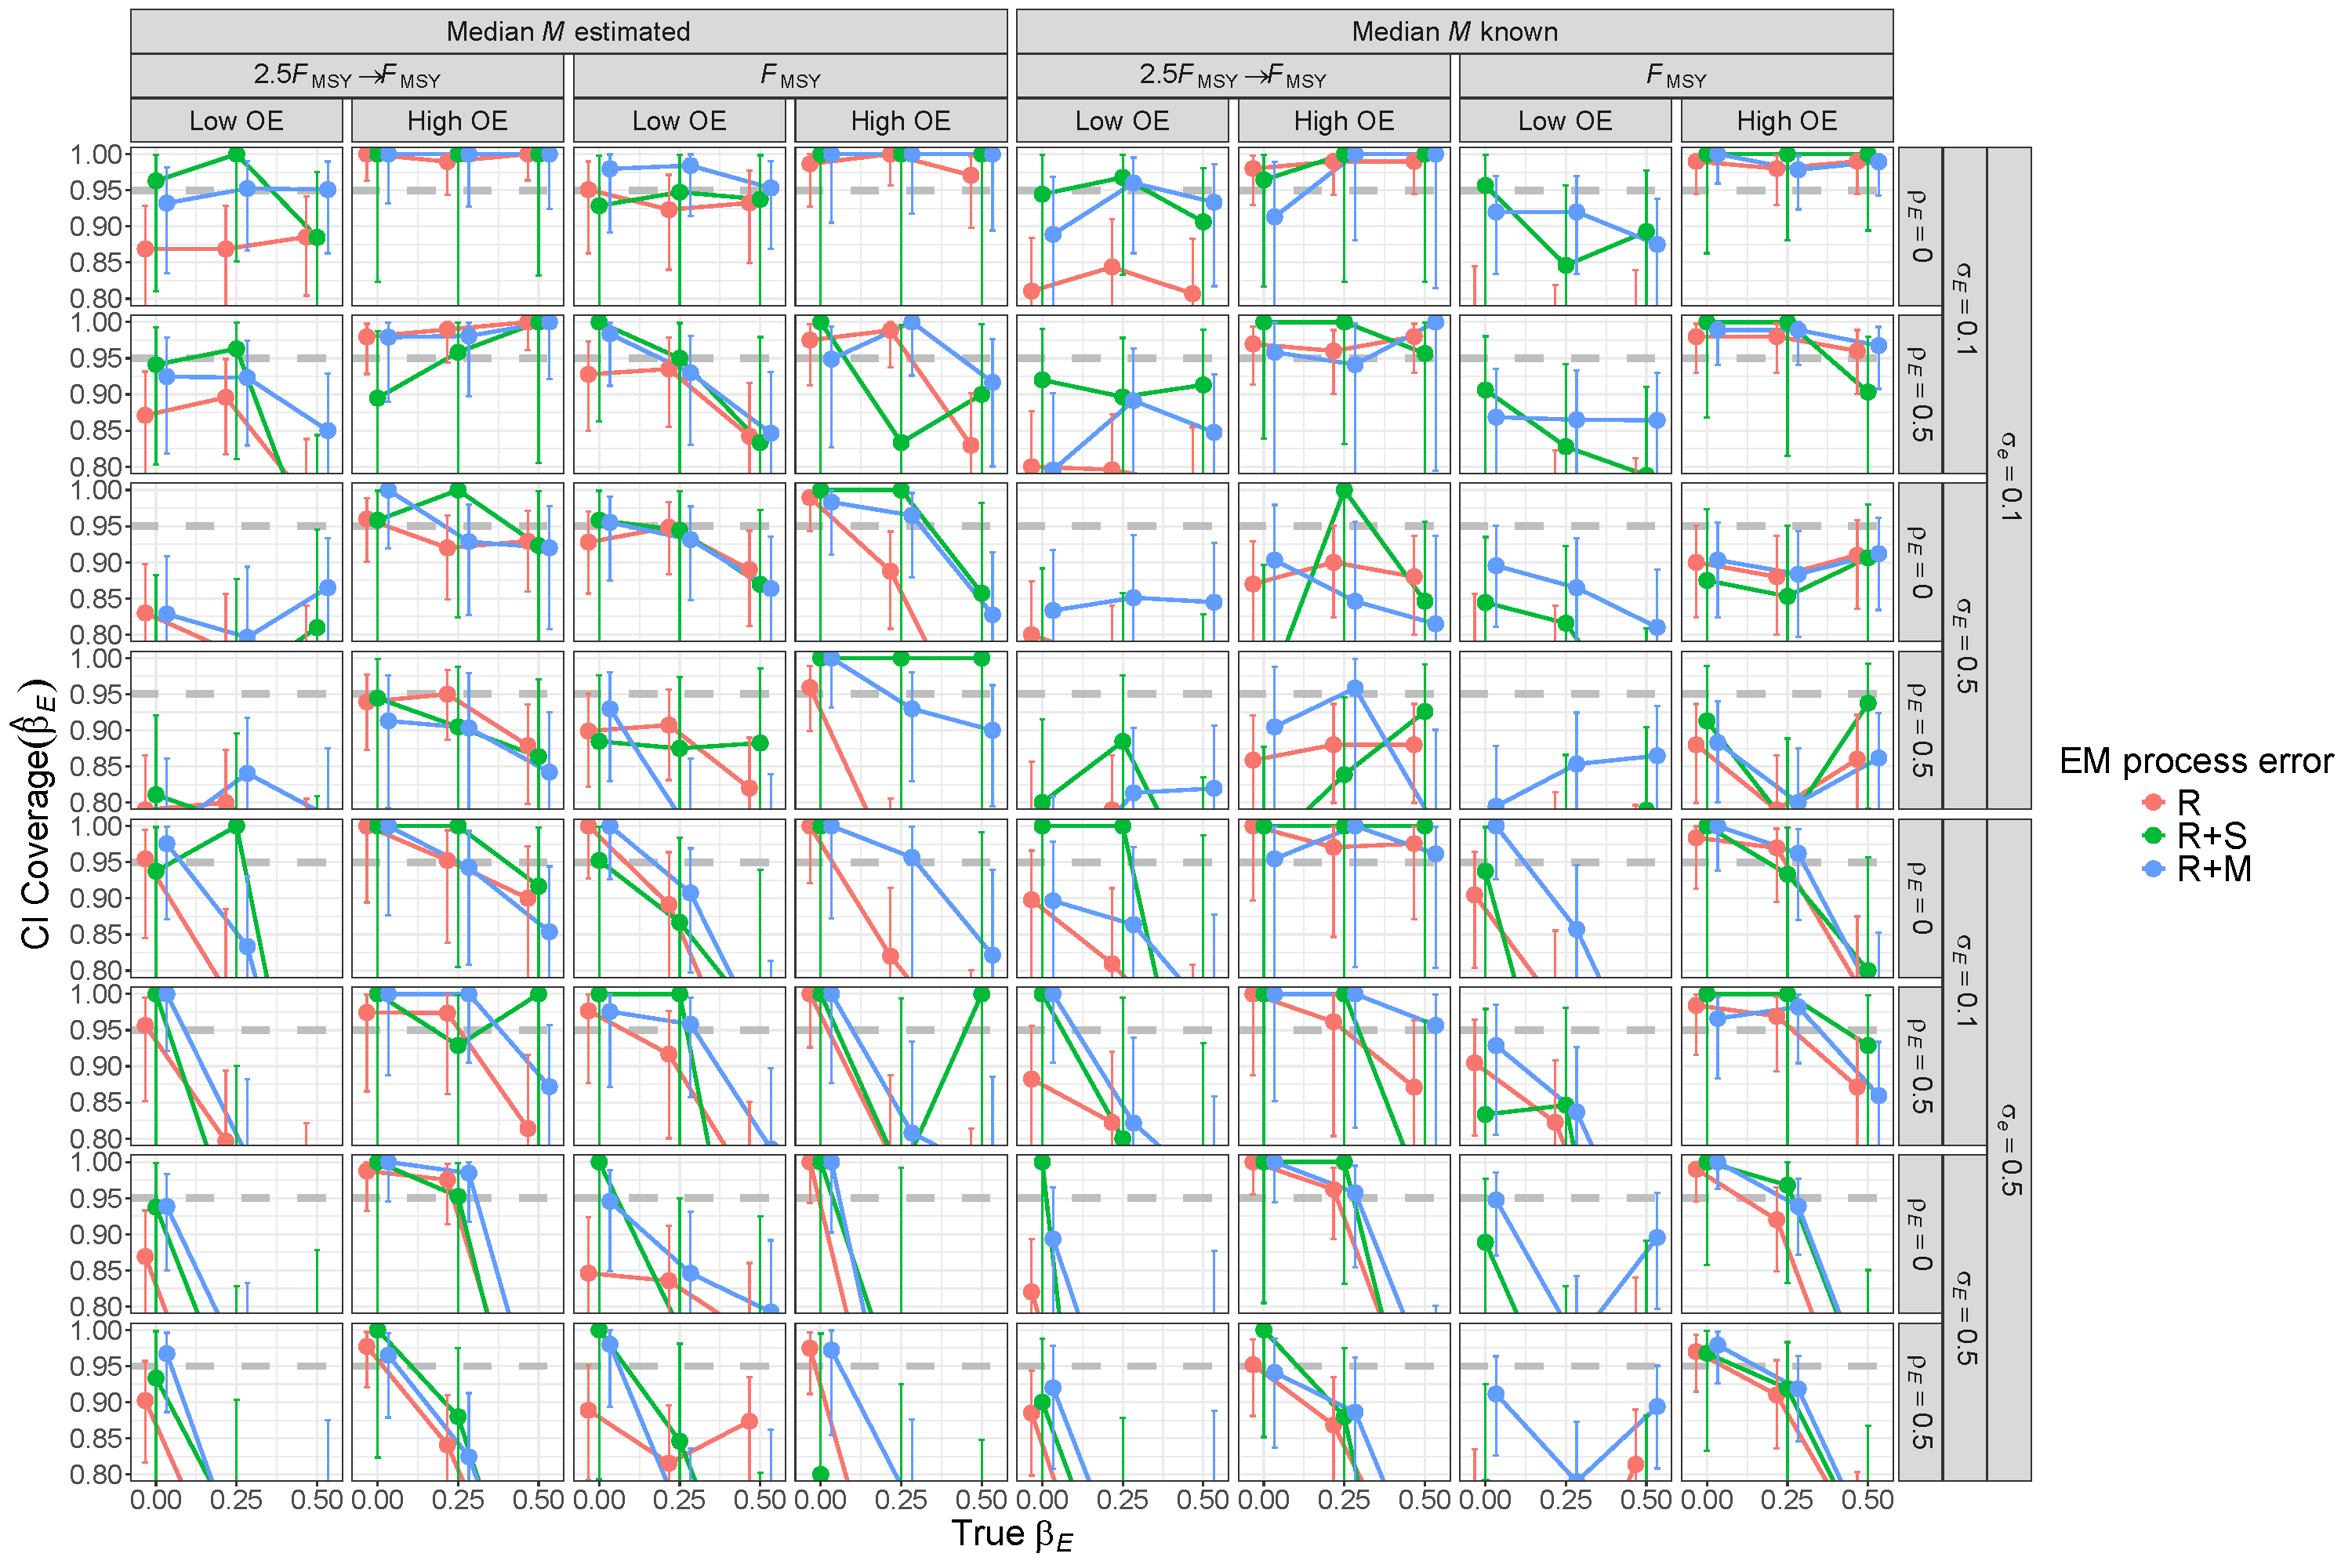
\includegraphics[height = \textheight]{beta_E_CI_coverage_RMom}
\end{center}
\caption{\DIFaddFL{For R+M operating models, probability of 95\% confidence interval for $\beta_E$ containing the true value for estimating models with alternative process error assumptions and treatment of median $M$ parameter ($\beta_M$). Vertical lines represent 95\% confidence intervals.}}\label{beta_E_CI_coverage_RMom}
\end{figure}
\end{landscape}

\begin{landscape}
\begin{figure}
\begin{center}
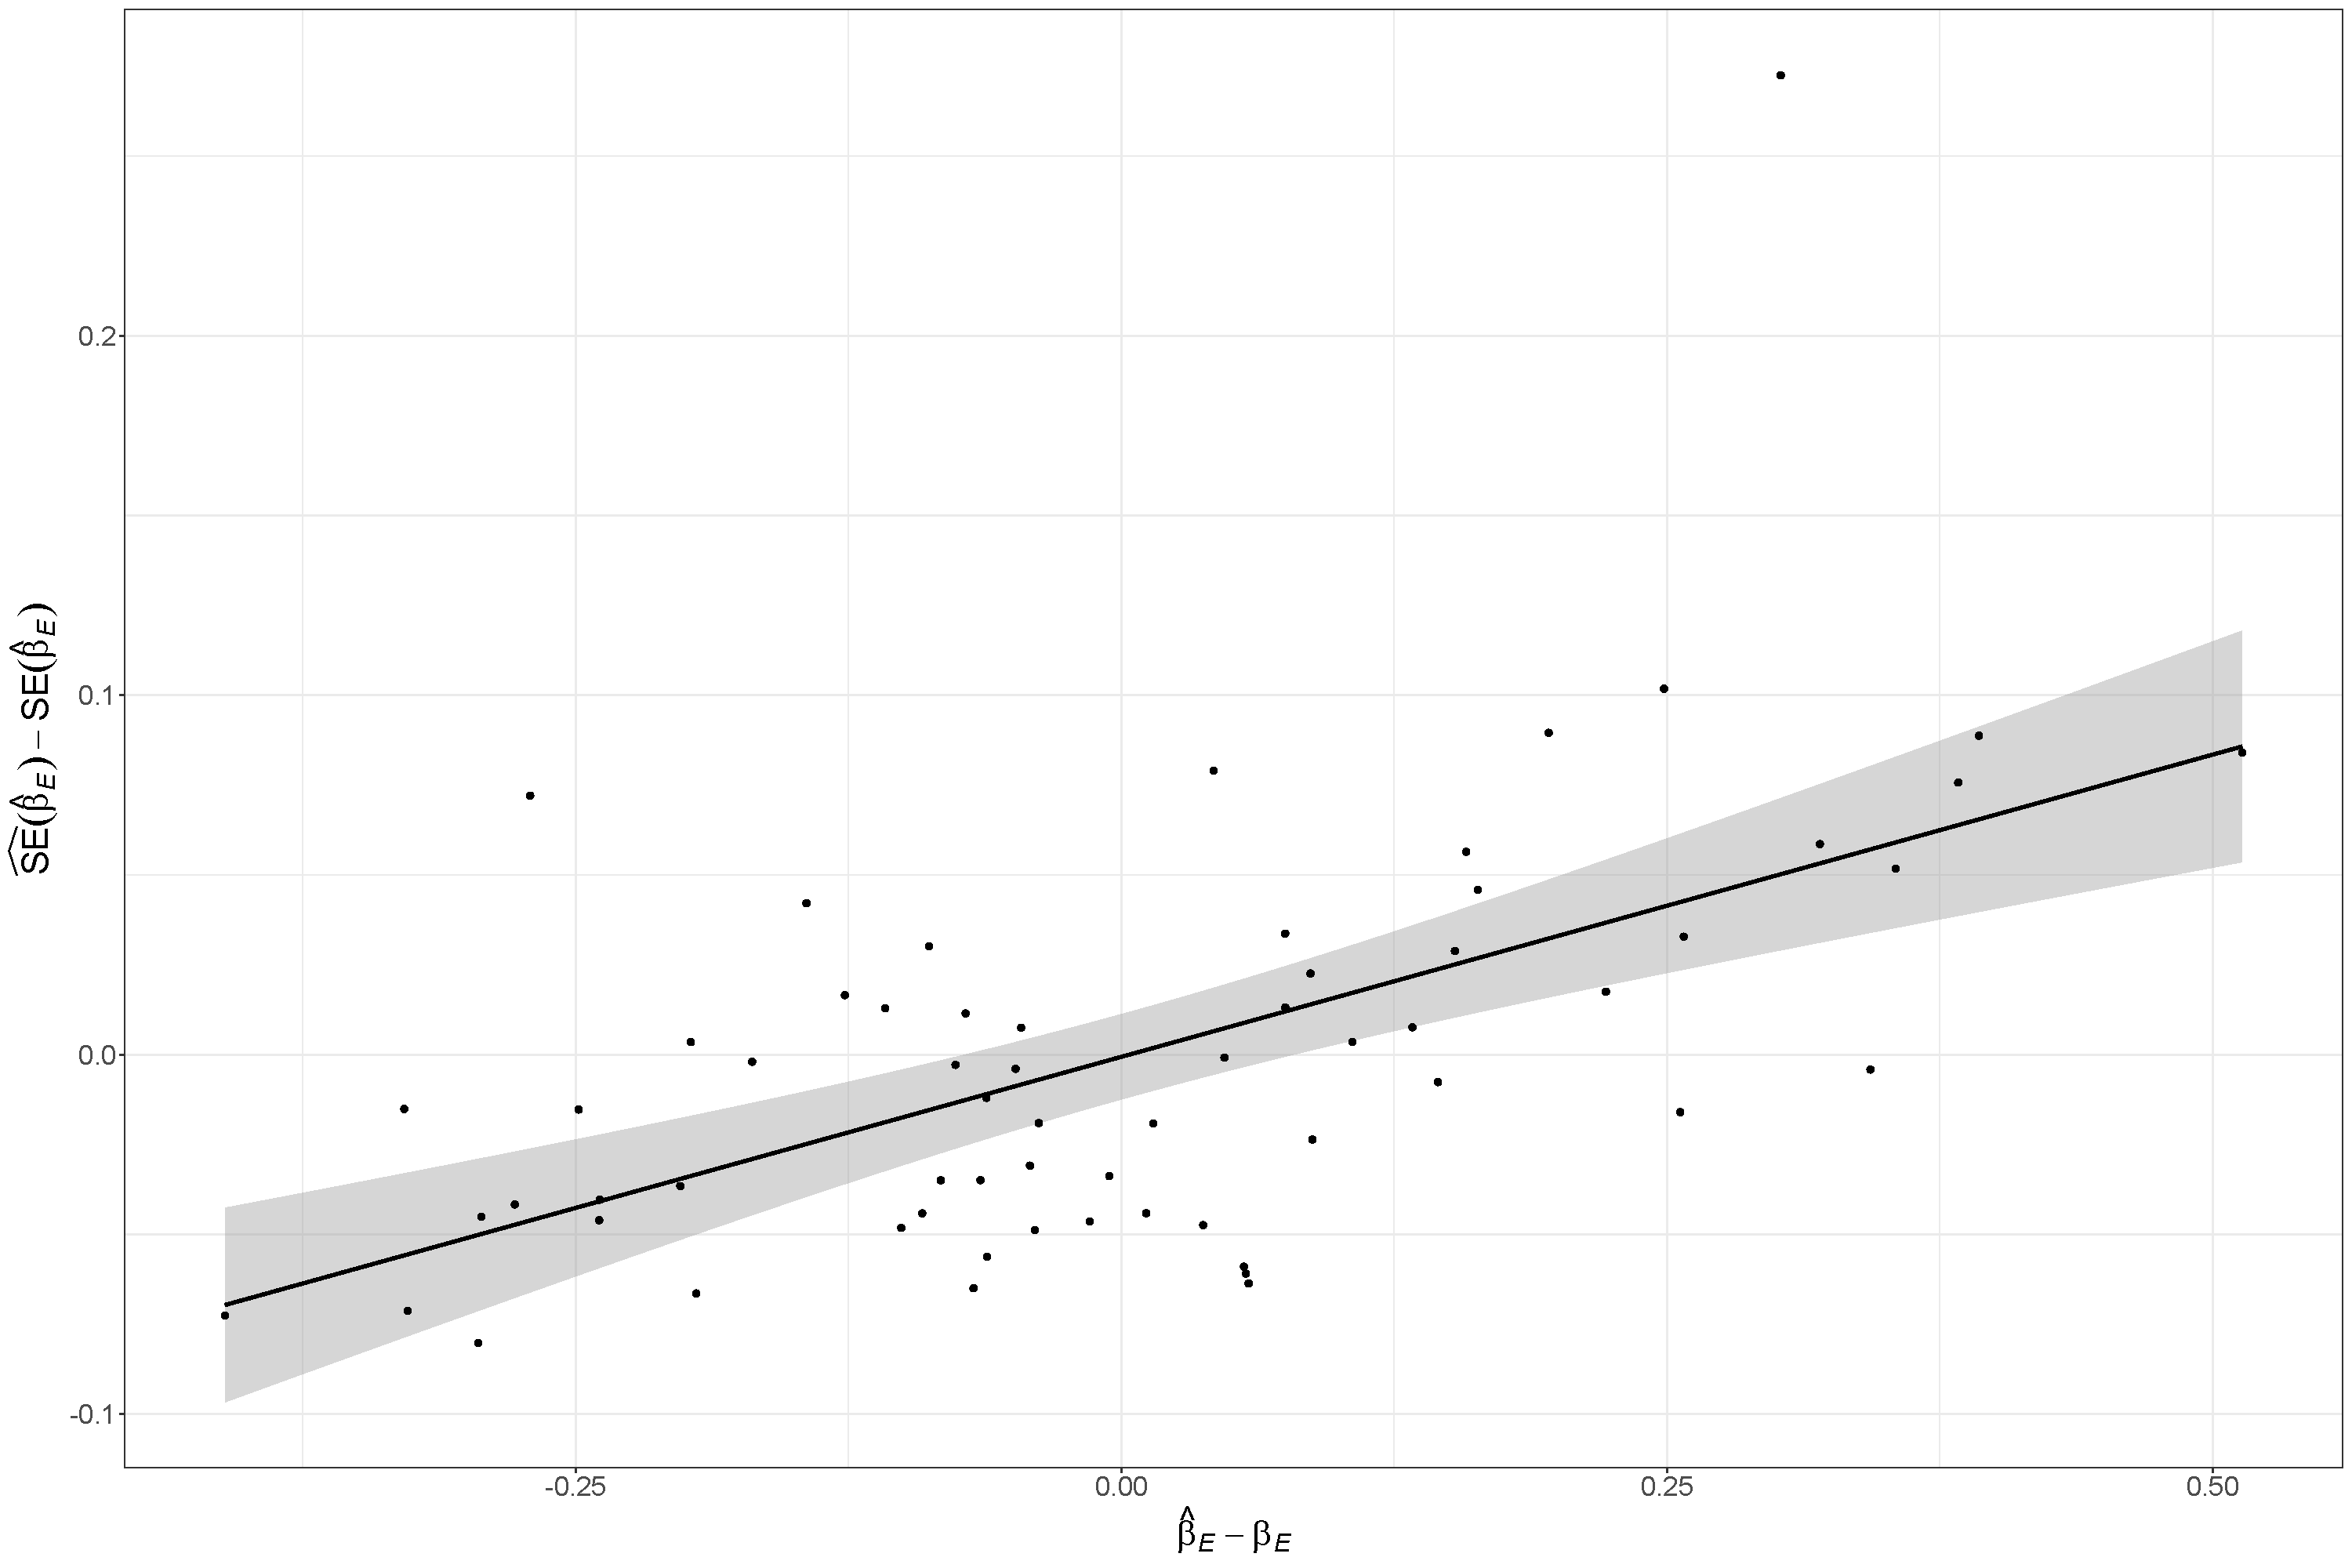
\includegraphics[height = 0.9\textheight]{om_69_em_5_beta_E_se_beta_E_lm_plot}
\end{center}
\caption{\DIFaddFL{Positive correlation of covariate effect estimates and Hessian-based standard error estimates for estimating model that also estimates the median $M$ parameter ($\beta_M$) and has correct R+M process error assumption fitted to simulated data from the operating model with R+M process errors, temporal contrast in fishing pressure, low observation uncertainty for both population ($Low OE$) and covariate observations ($\sigma_e = 0.1$), high and uncorrelated temporal variability in the true covariate ($\sigma_E = 0.5$ and $\rho_E = 0$), and the strongest covariate effect on $M$ ($\beta_E = 0.5$).}}\label{ex_lm_beta_E_SE_beta_E}
\end{figure}
\end{landscape}

\begin{landscape}
\begin{figure}
\begin{center}
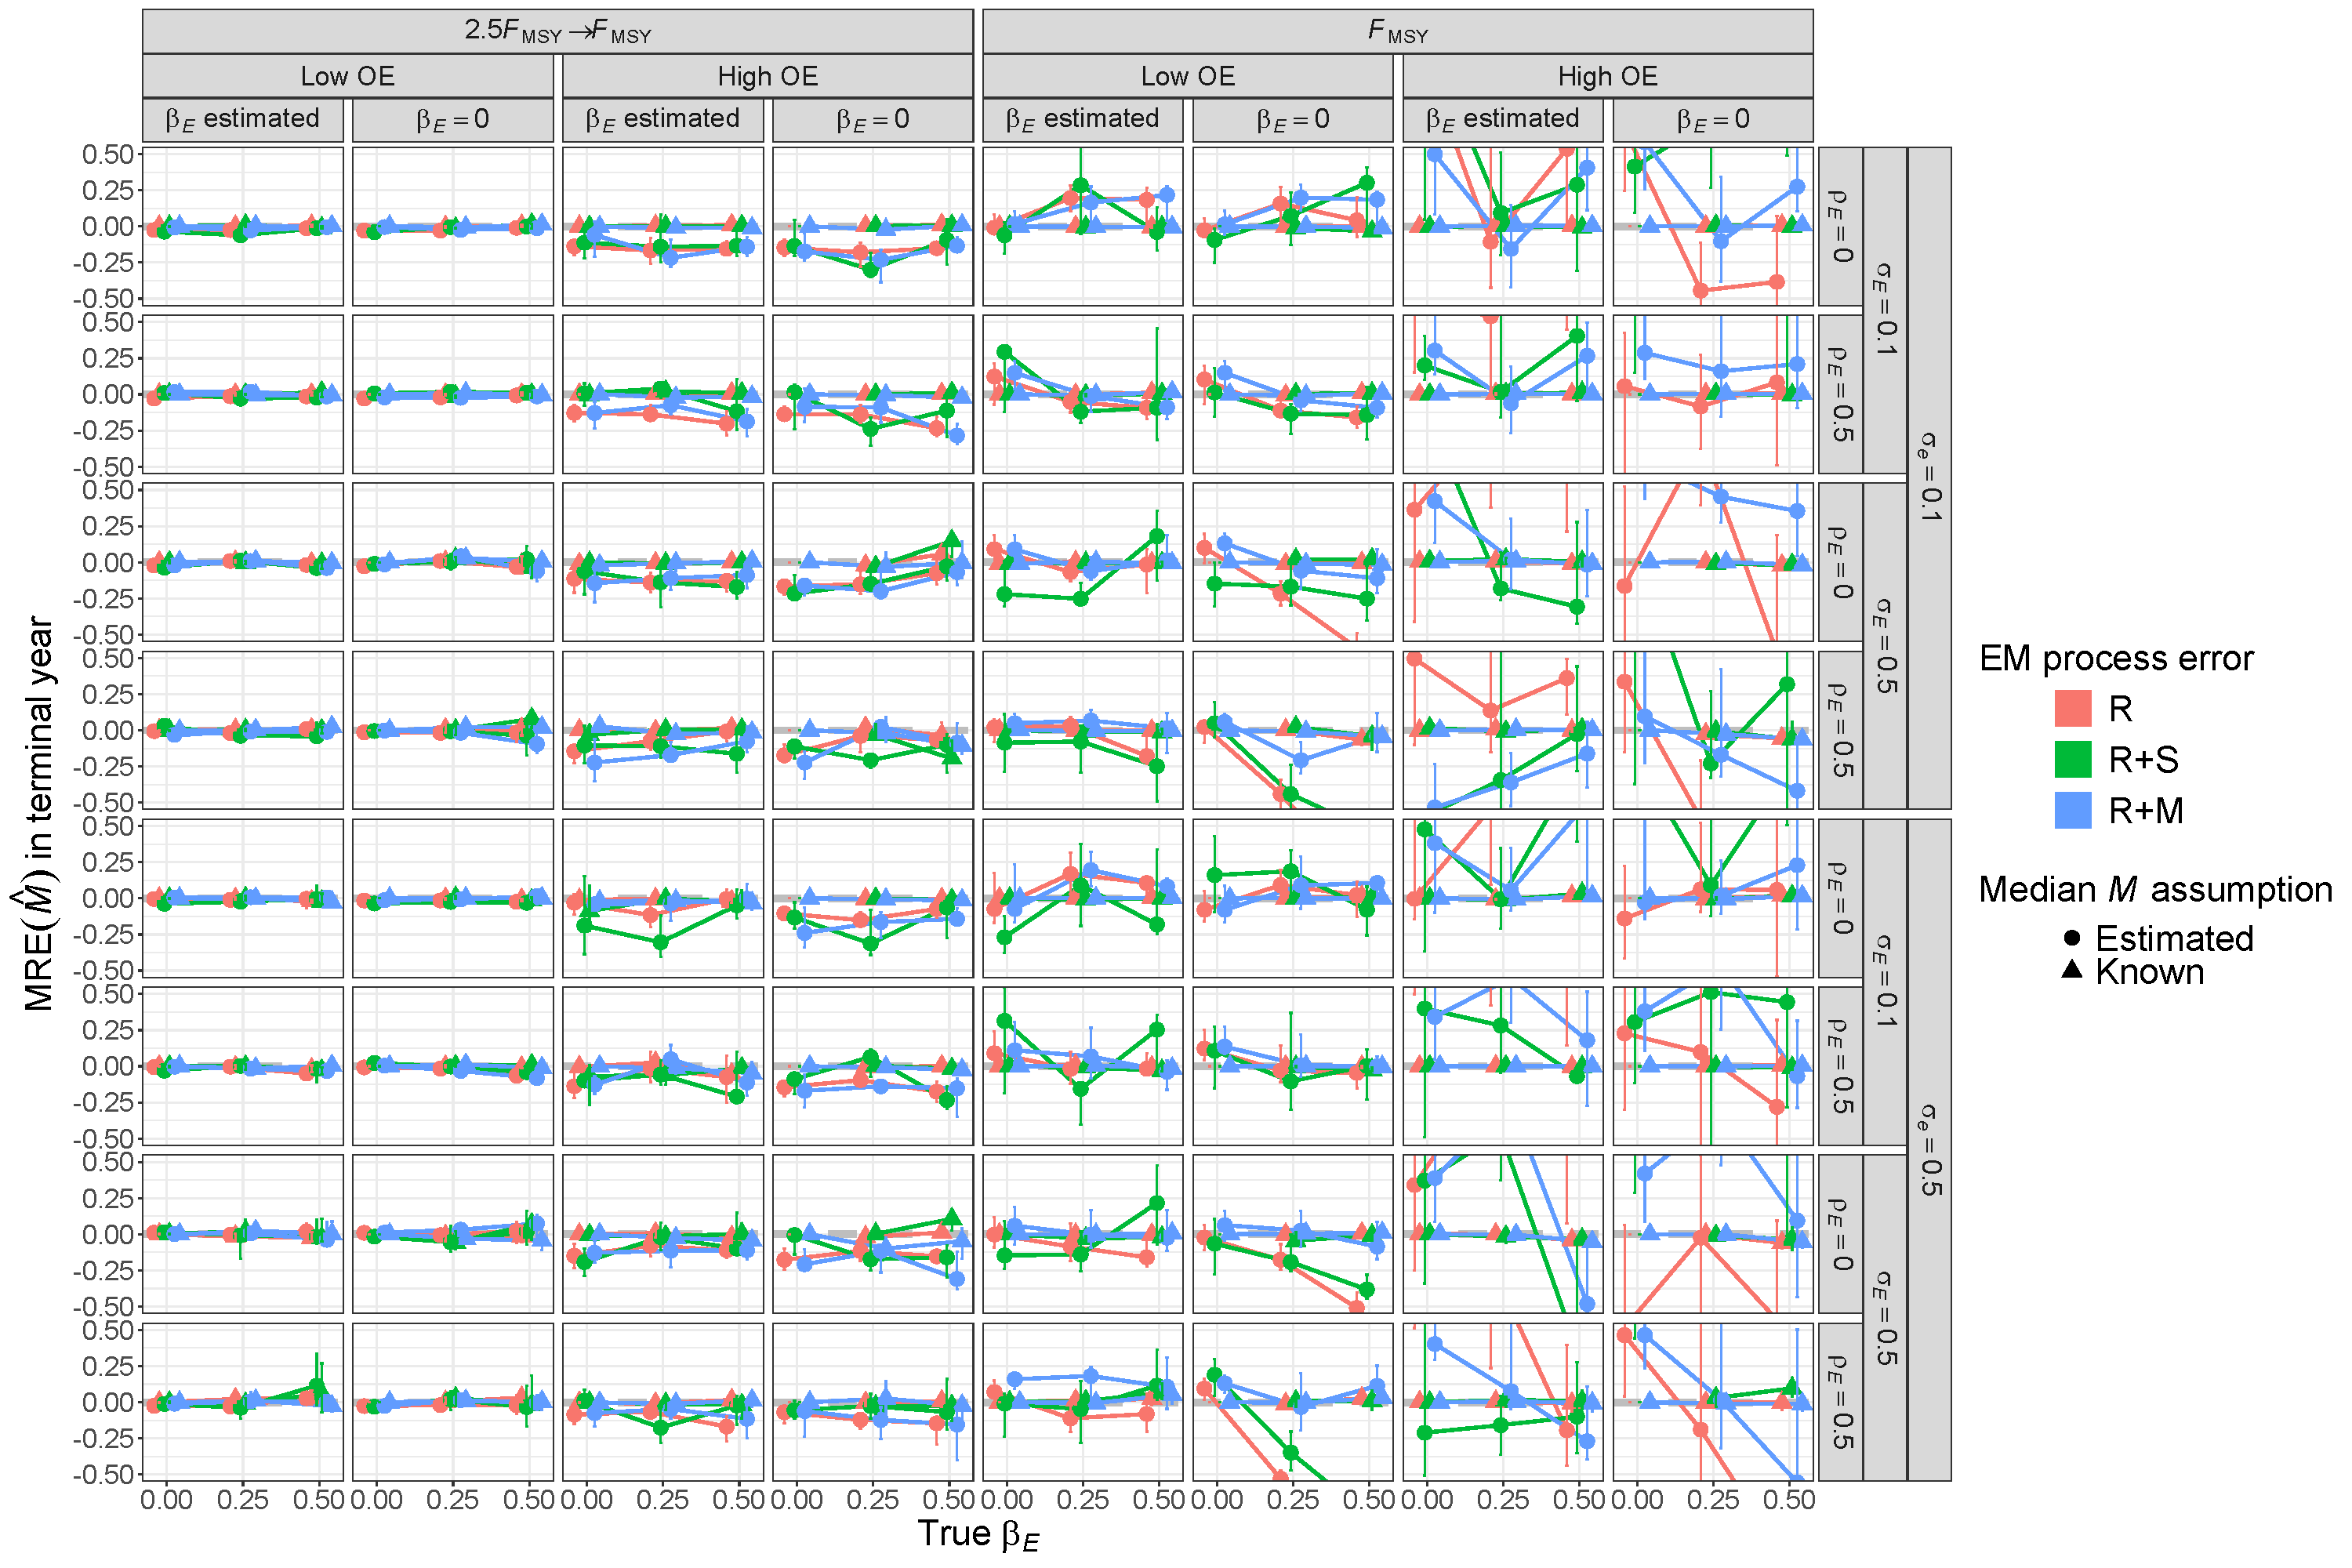
\includegraphics[height = \textheight]{terminal_year_M_bias_Rom}
\end{center}
\caption{\DIFaddFL{For R operating models, median relative error (MRE) of estimates of terminal year $M$ for estimating models with alternative process error assumptions, treatment of covariate effect ($\beta_E = 0$ or estimated), and treatment of median $M$ parameter ($\beta_M$ estimated or known).}}\label{terminal_M_bias_Rom}
\end{figure}
\end{landscape}

\begin{landscape}
\begin{figure}
\begin{center}
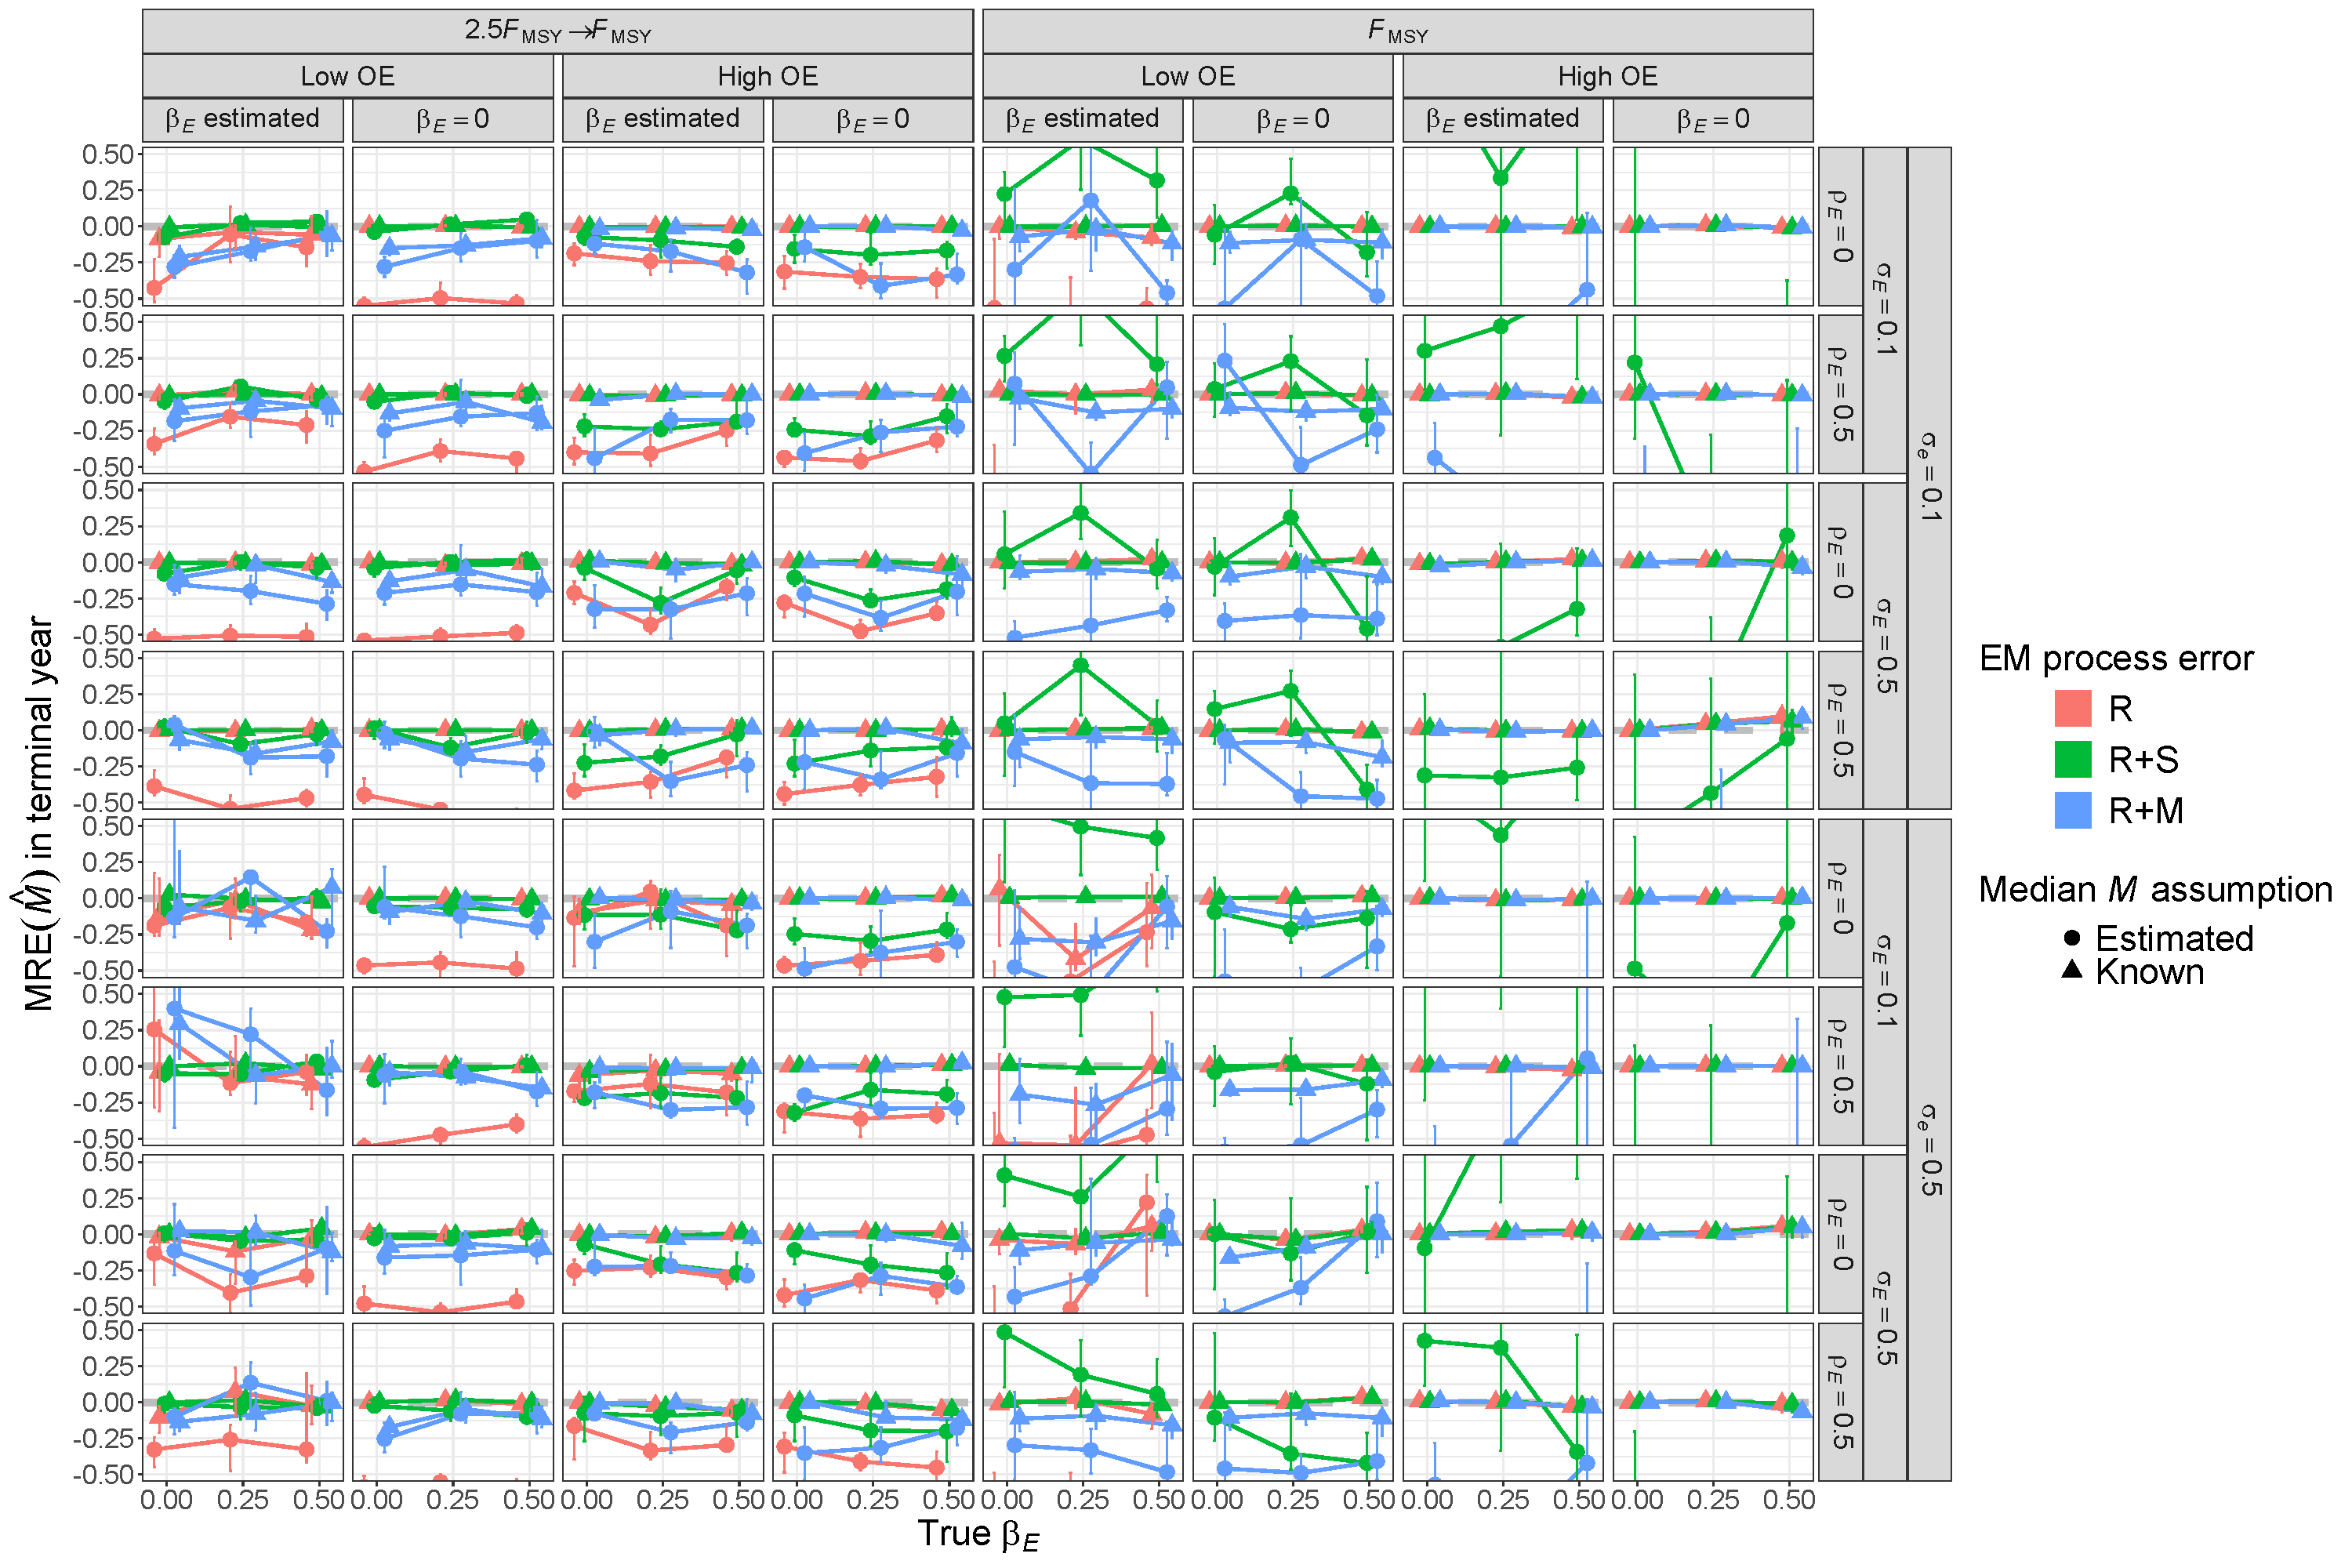
\includegraphics[height = \textheight]{terminal_year_M_bias_RSom}
\end{center}
\caption{\DIFaddFL{For R+S operating models, median relative error (MRE) of estimates of terminal year $M$ for estimating models with alternative process error assumptions, treatment of covariate effect ($\beta_E = 0$ or estimated), and treatment of median $M$ parameter ($\beta_M$ estimated or known).}}\label{terminal_M_bias_RSom}
\end{figure}
\end{landscape}

\begin{landscape}
\begin{figure}
\begin{center}
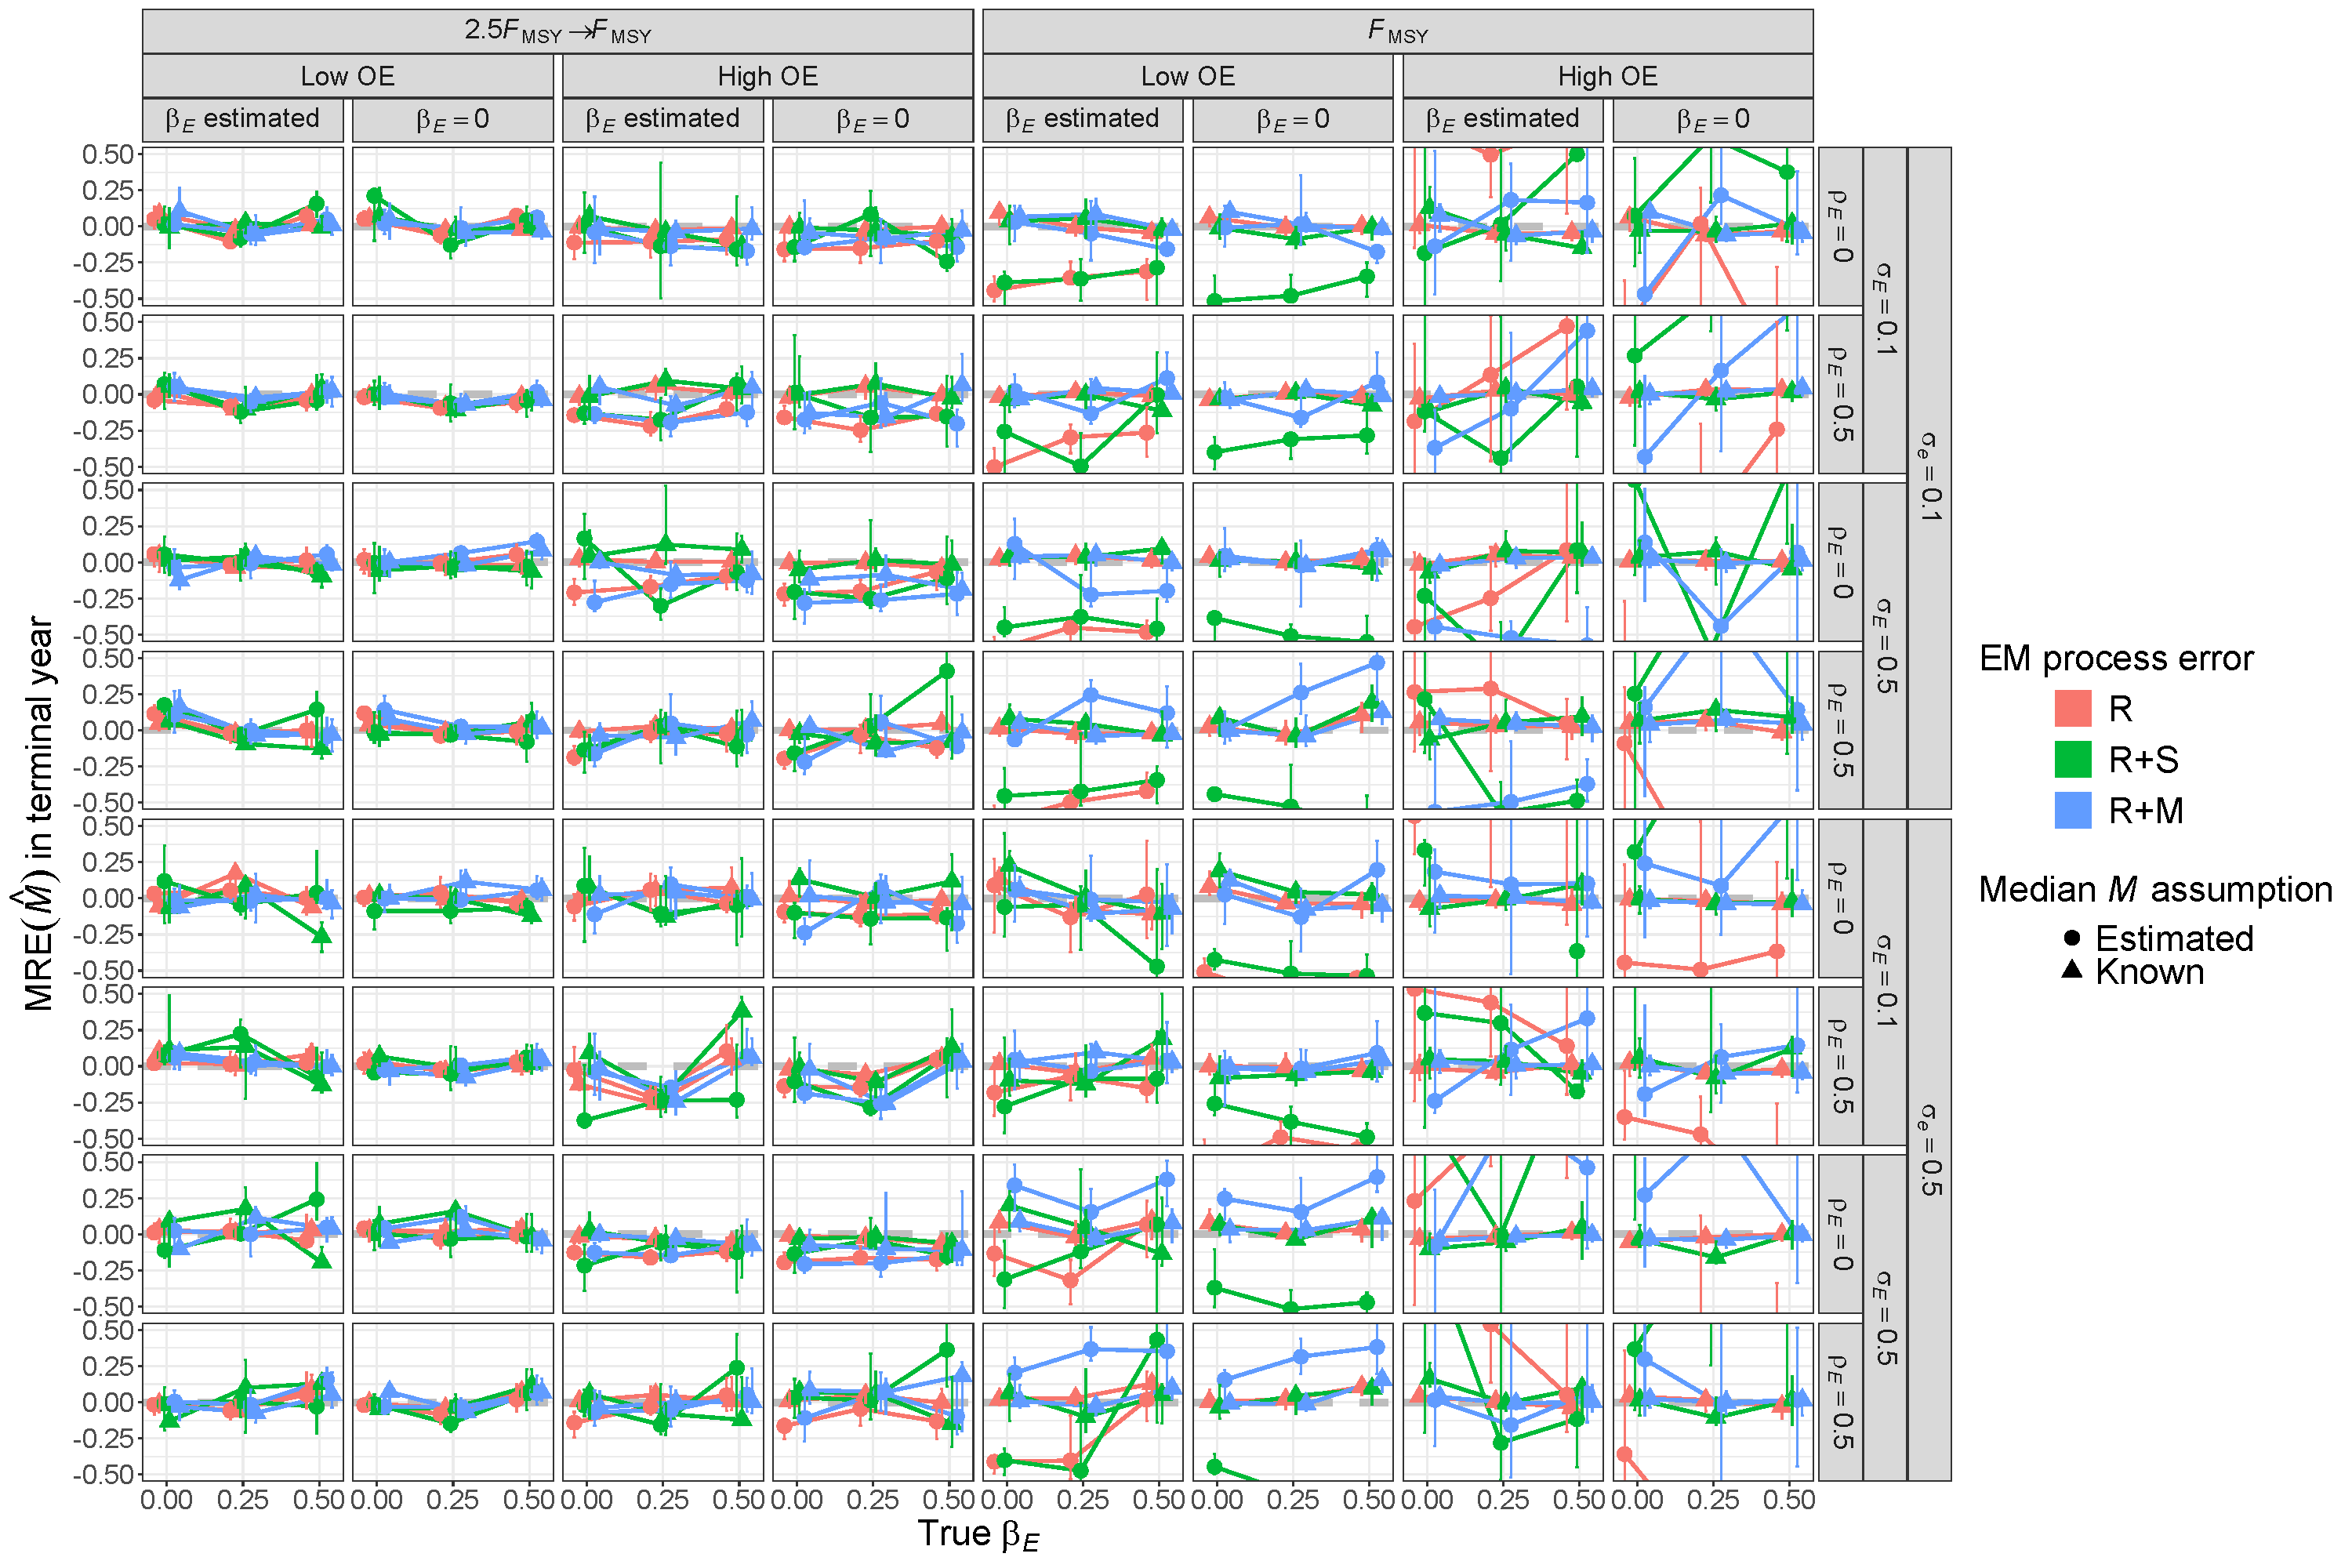
\includegraphics[height = \textheight]{terminal_year_M_bias_RMom}
\end{center}
\caption{\DIFaddFL{For R+M operating models, median relative error (MRE) of estimates of terminal year $M$ for estimating models with alternative process error assumptions, treatment of covariate effect ($\beta_E = 0$ or estimated), and treatment of median $M$ parameter ($\beta_M$ estimated or known).}}\label{terminal_M_bias_RMom}
\end{figure}
\end{landscape}

\begin{landscape}
\begin{figure}
\begin{center}
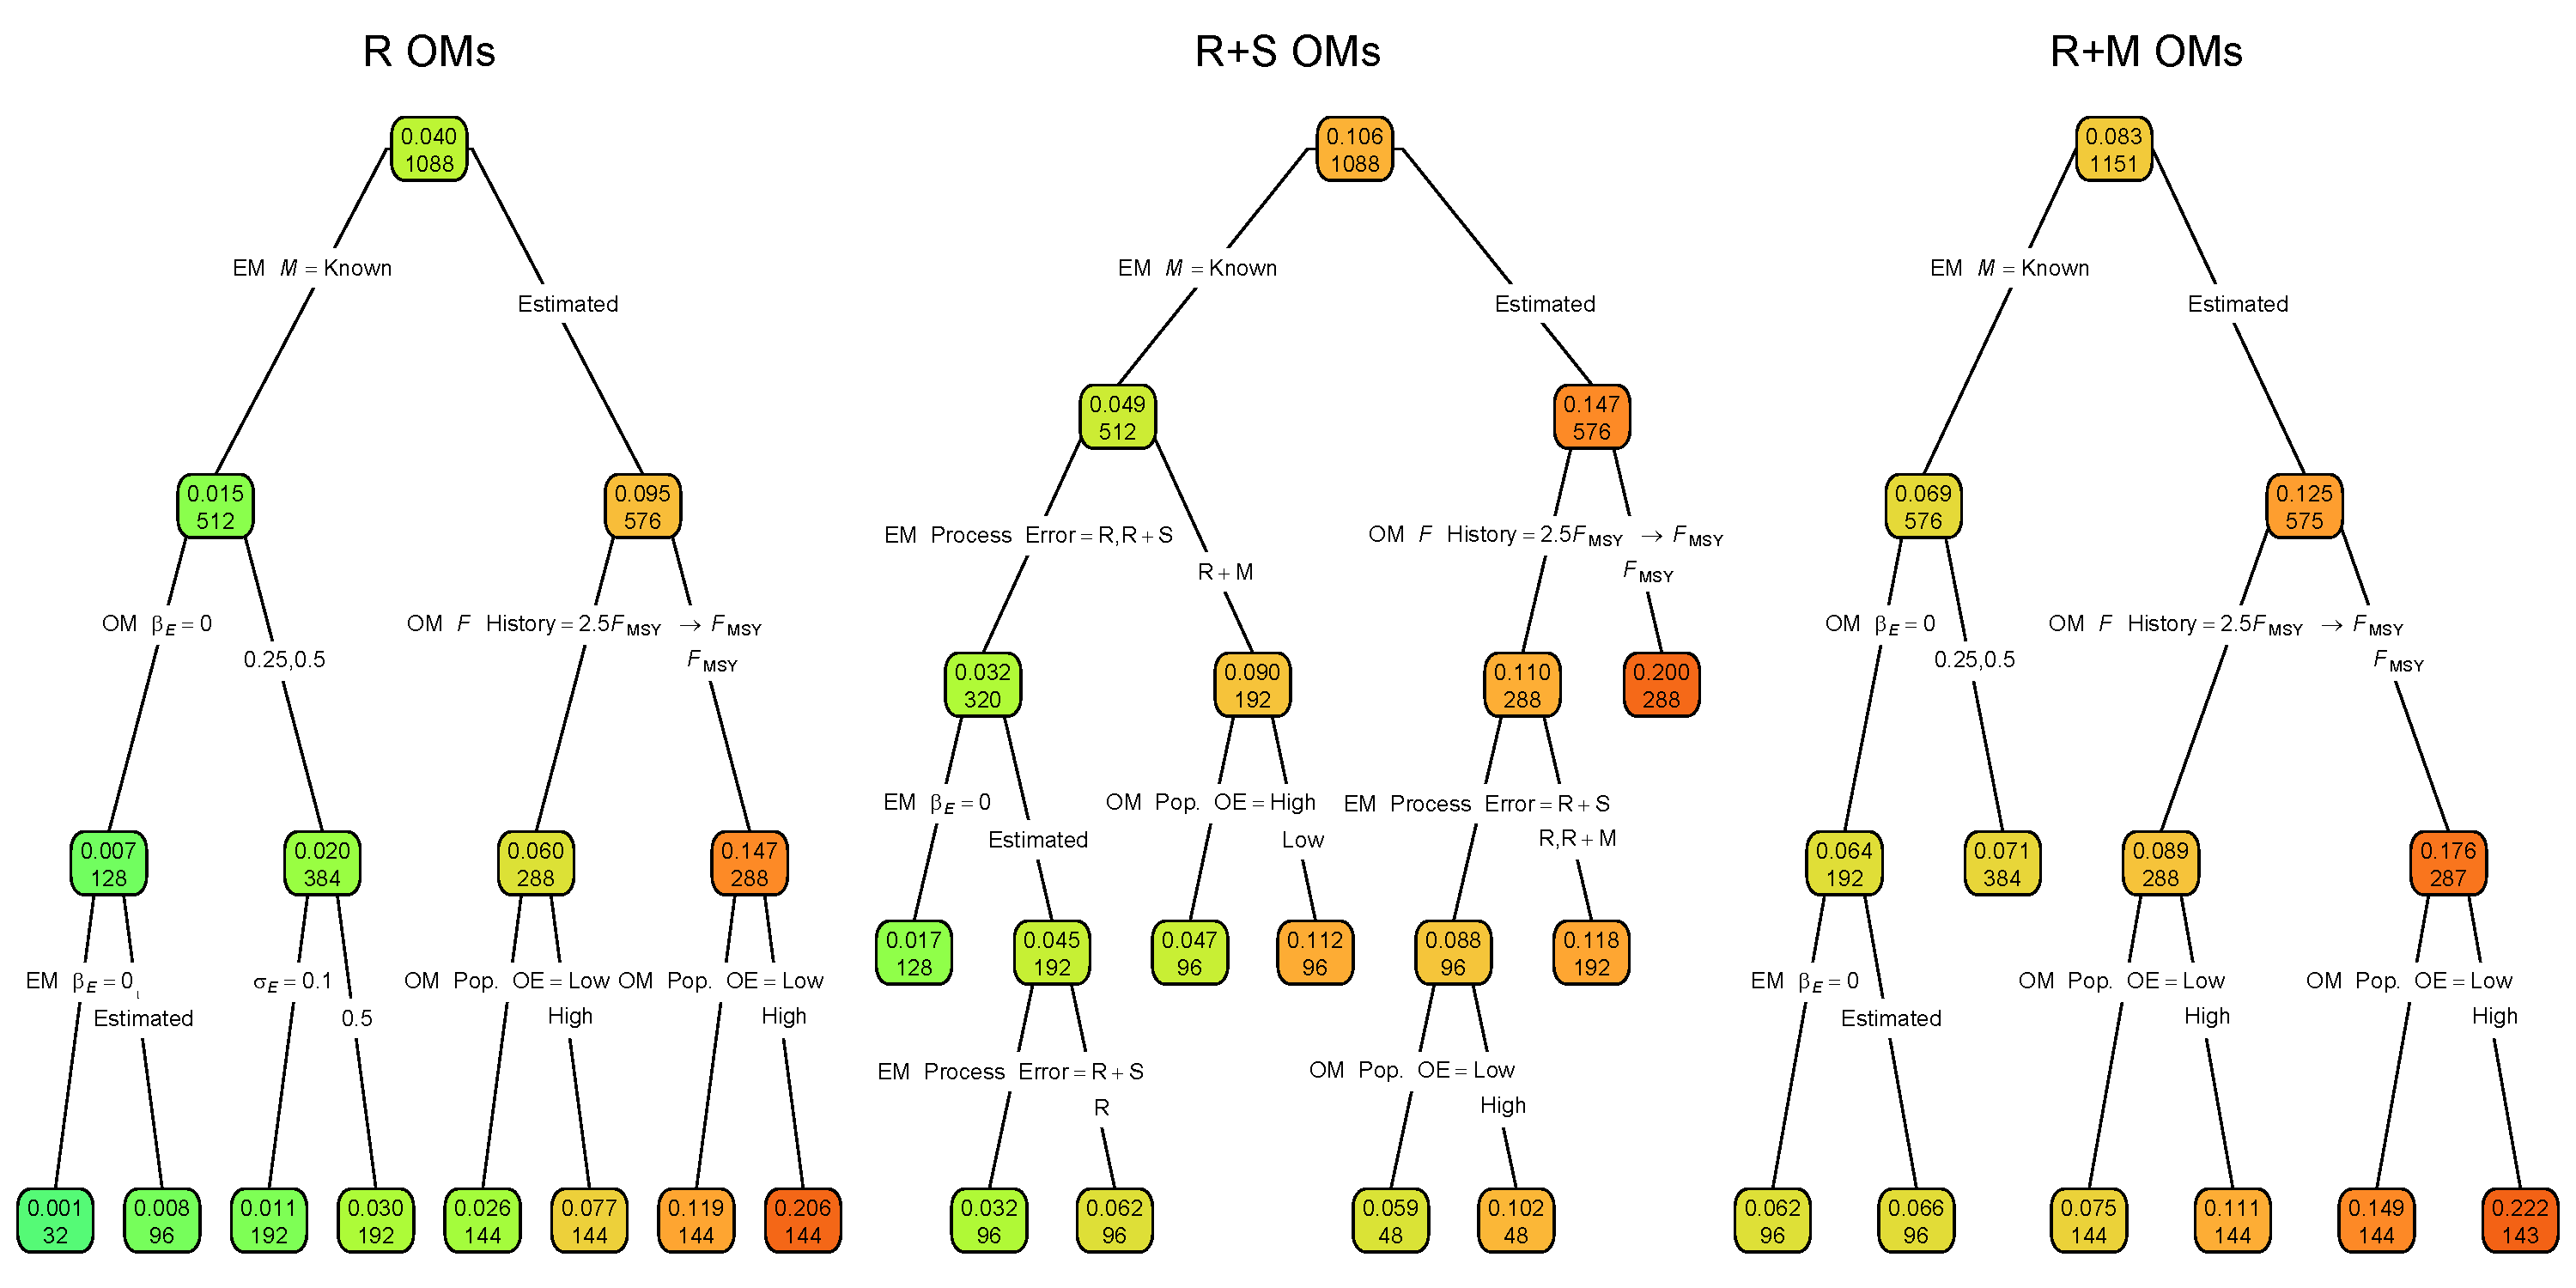
\includegraphics[width = 1.4\textwidth]{term_M_rmse_regtree_plots}
\end{center}
\caption{\DIFaddFL{Regression trees for the log-transformed RMSE of terminal year $M$. Each node shows the median RMSE (top) and number of observations (bottom) for the corresponding subset. Lower or higher median RMSE are indicated by more green or red polygons, respectively. See Figure \ref{conv_class} caption and Table \ref{factor_table} for further details.}}\label{term_M_rmse_regtree}
\end{figure}
\end{landscape}

\begin{landscape}
\begin{figure}
\begin{center}
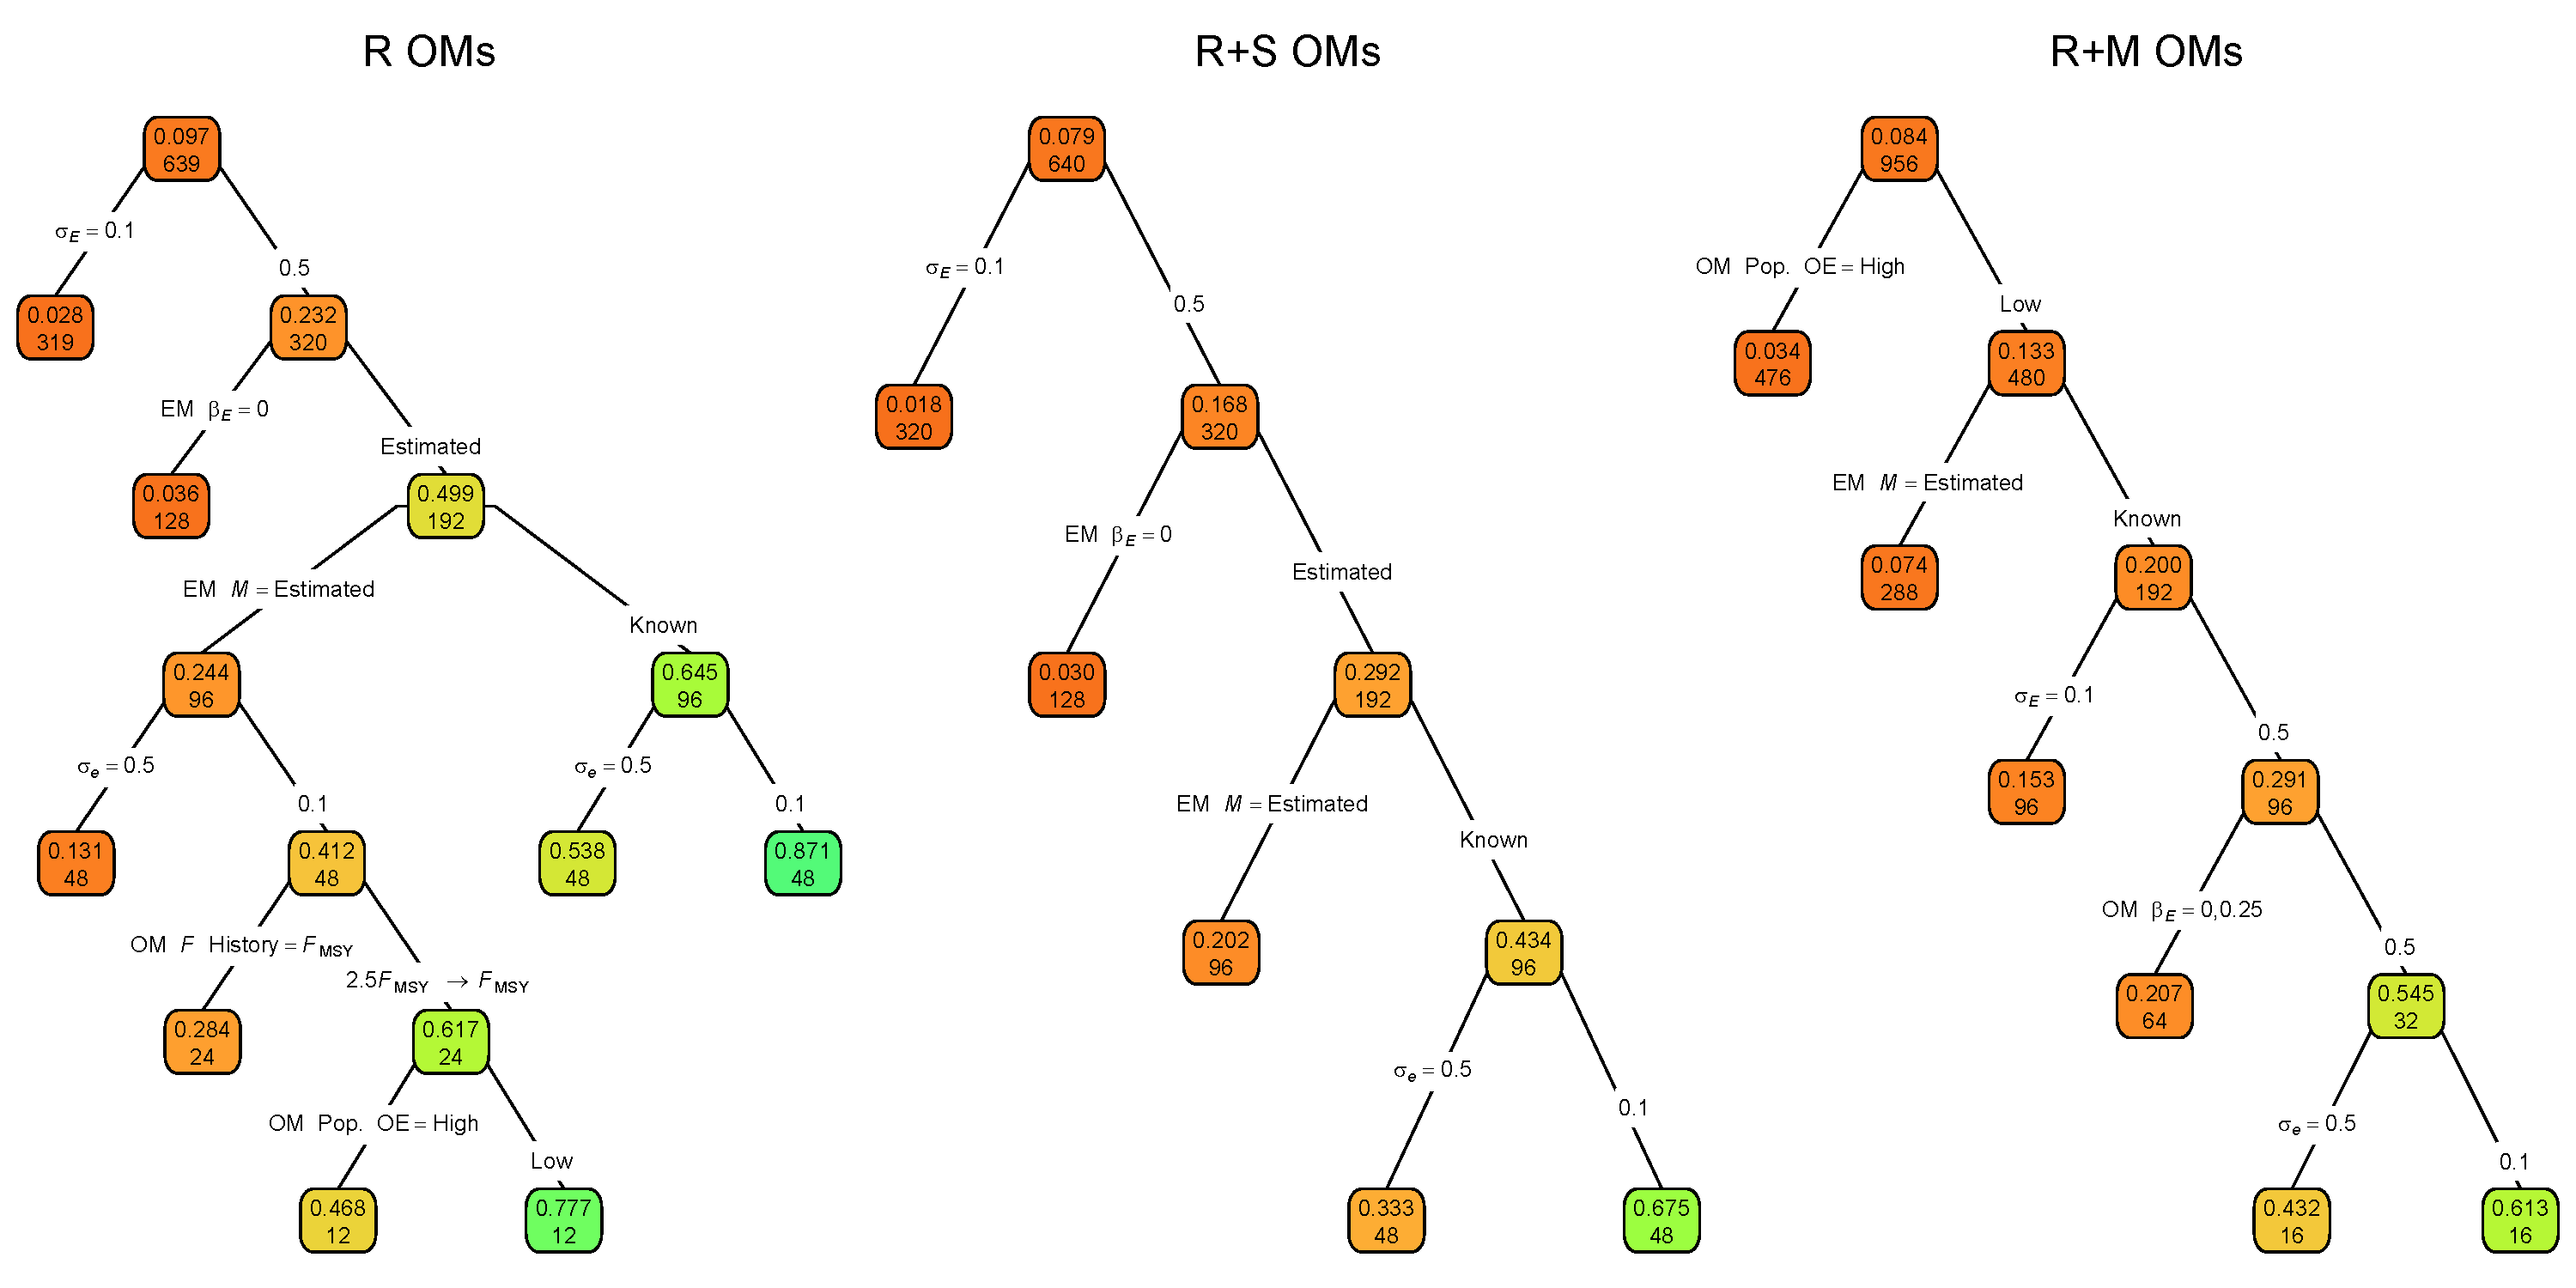
\includegraphics[width = 1.4\textwidth]{term_M_corr_regtree_plots}
\end{center}
\caption{\DIFaddFL{Regression trees for the correlation of terminal year $M$ estimates and true values. Each node shows the median correlation for the corresponding subset. Lower or higher median correlations are indicated by more red or green polygons, respectively. See Figure \ref{conv_class} caption and Table \ref{factor_table} for further details.}}\label{term_M_corr_regtree}
\end{figure}
\end{landscape}

\begin{landscape}
\begin{figure}
\begin{center}
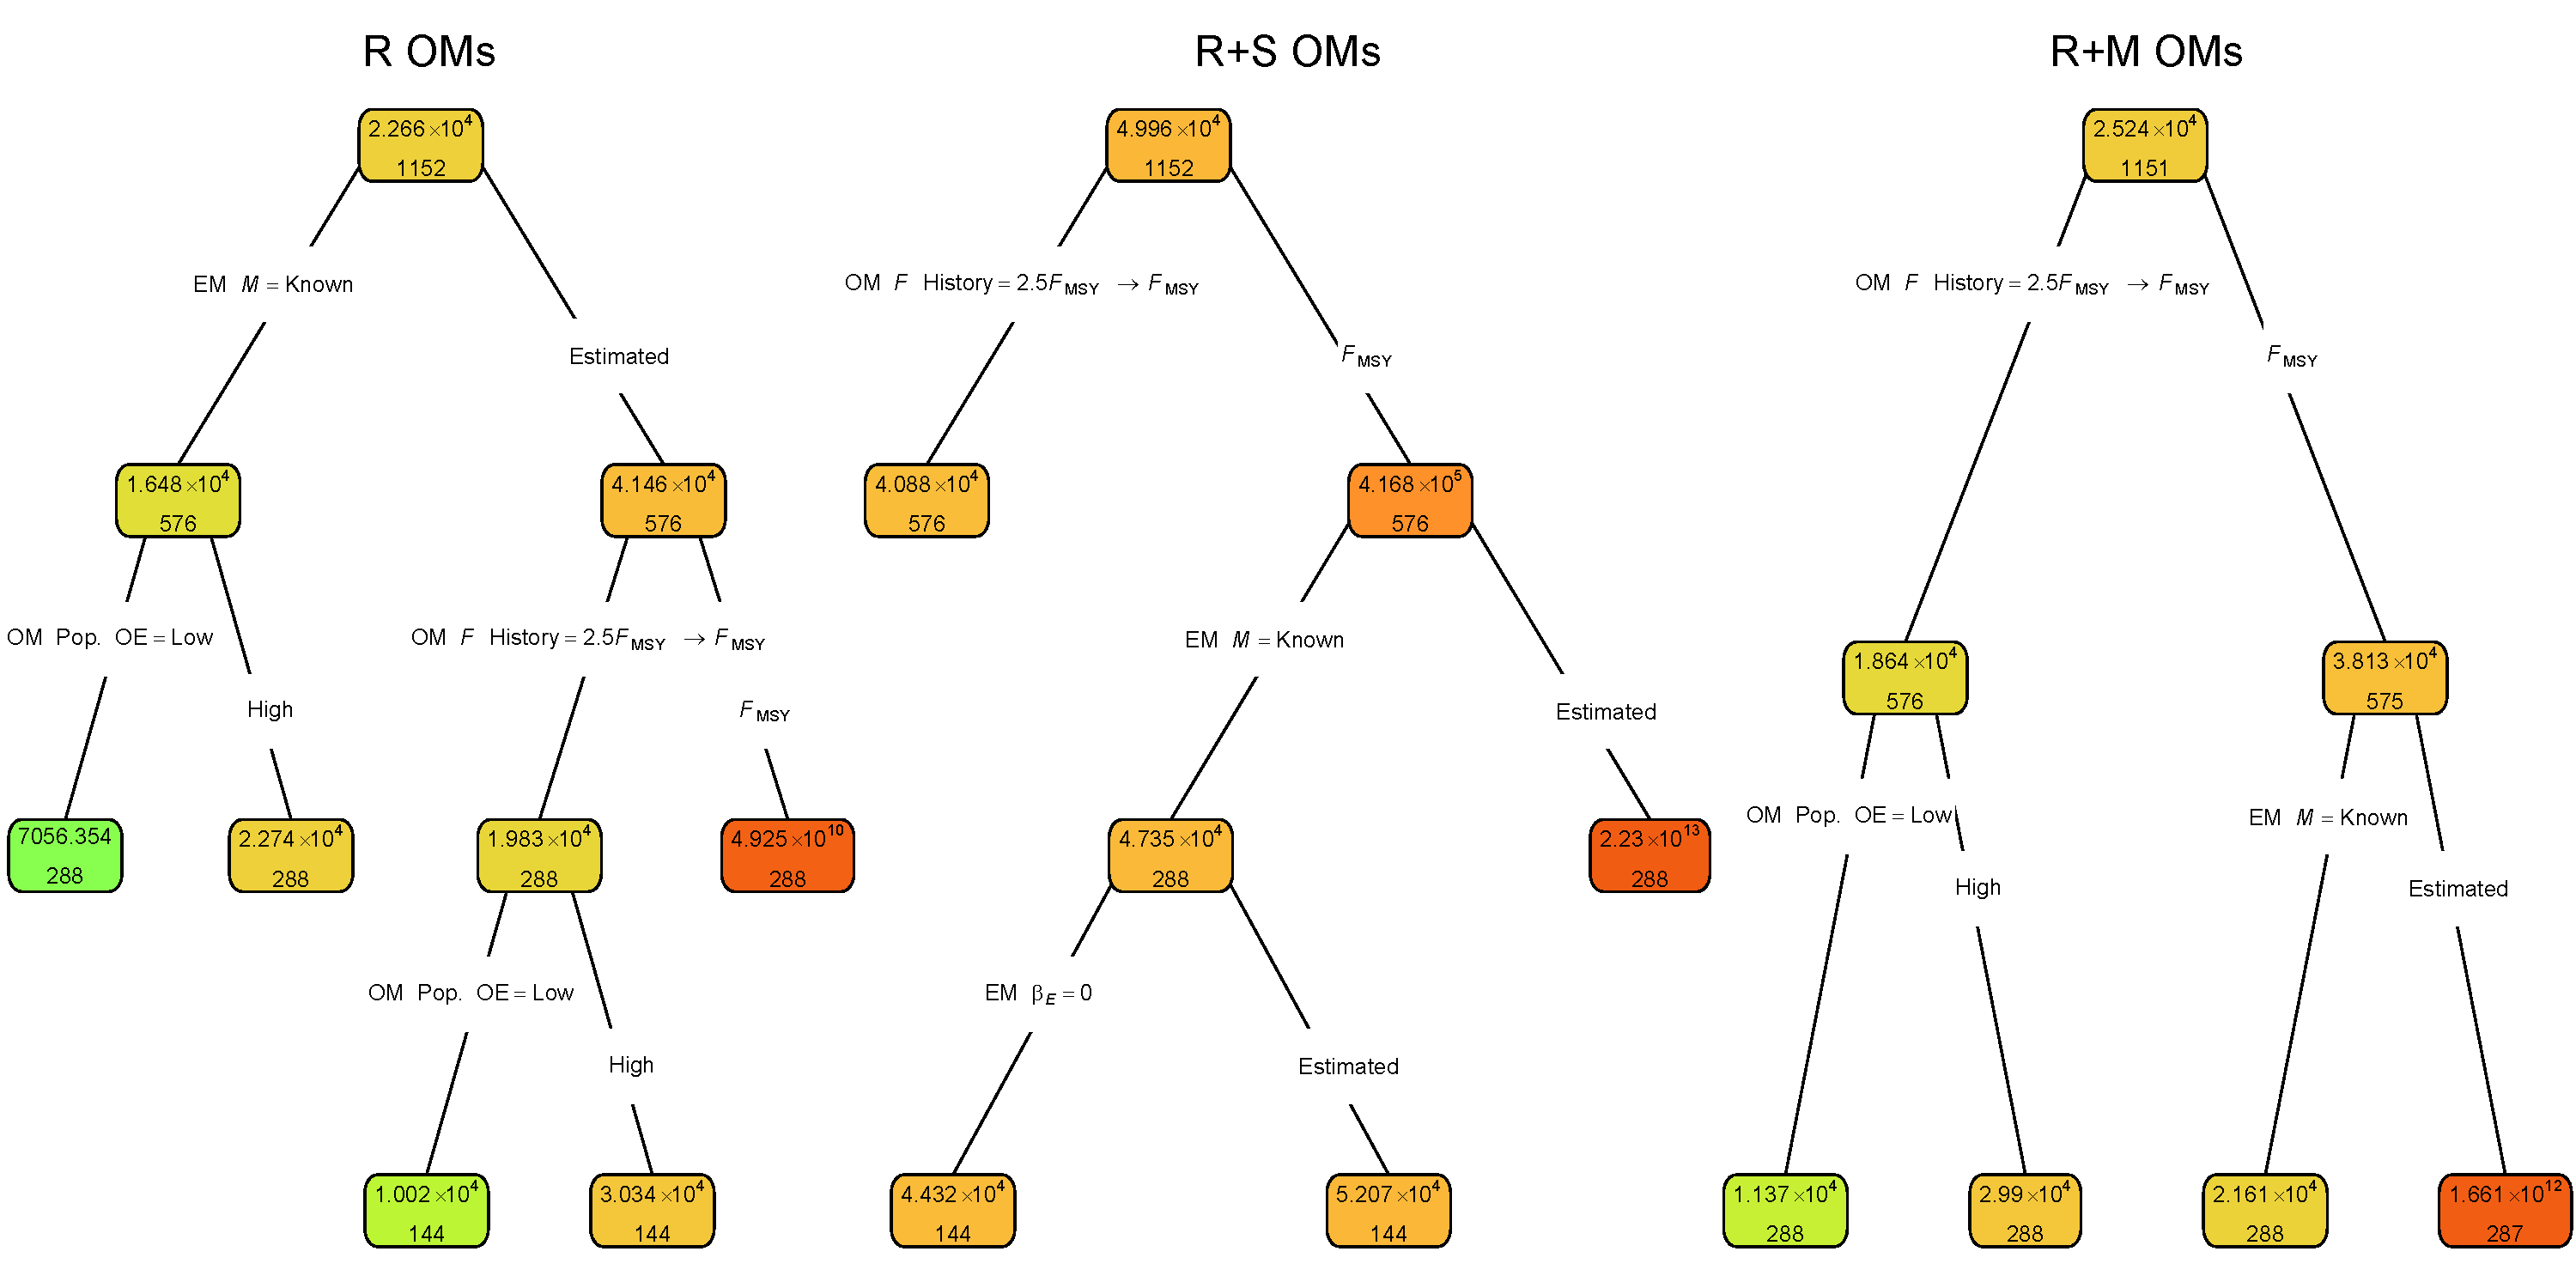
\includegraphics[width = 1.4\textwidth]{term_SSB_rmse_regtree_plots}
\end{center}
\caption{\DIFaddFL{Regression trees for the log-transformed RMSE of terminal year SSB. Each node shows the median RMSE (top) and number of observations (bottom) for the corresponding subset. Lower or higher median RMSE are indicated by more red or green polygons, respectively.}}\label{term_SSB_rmse_regtree}
\end{figure}
\end{landscape}

\begin{landscape}
\begin{figure}
\begin{center}
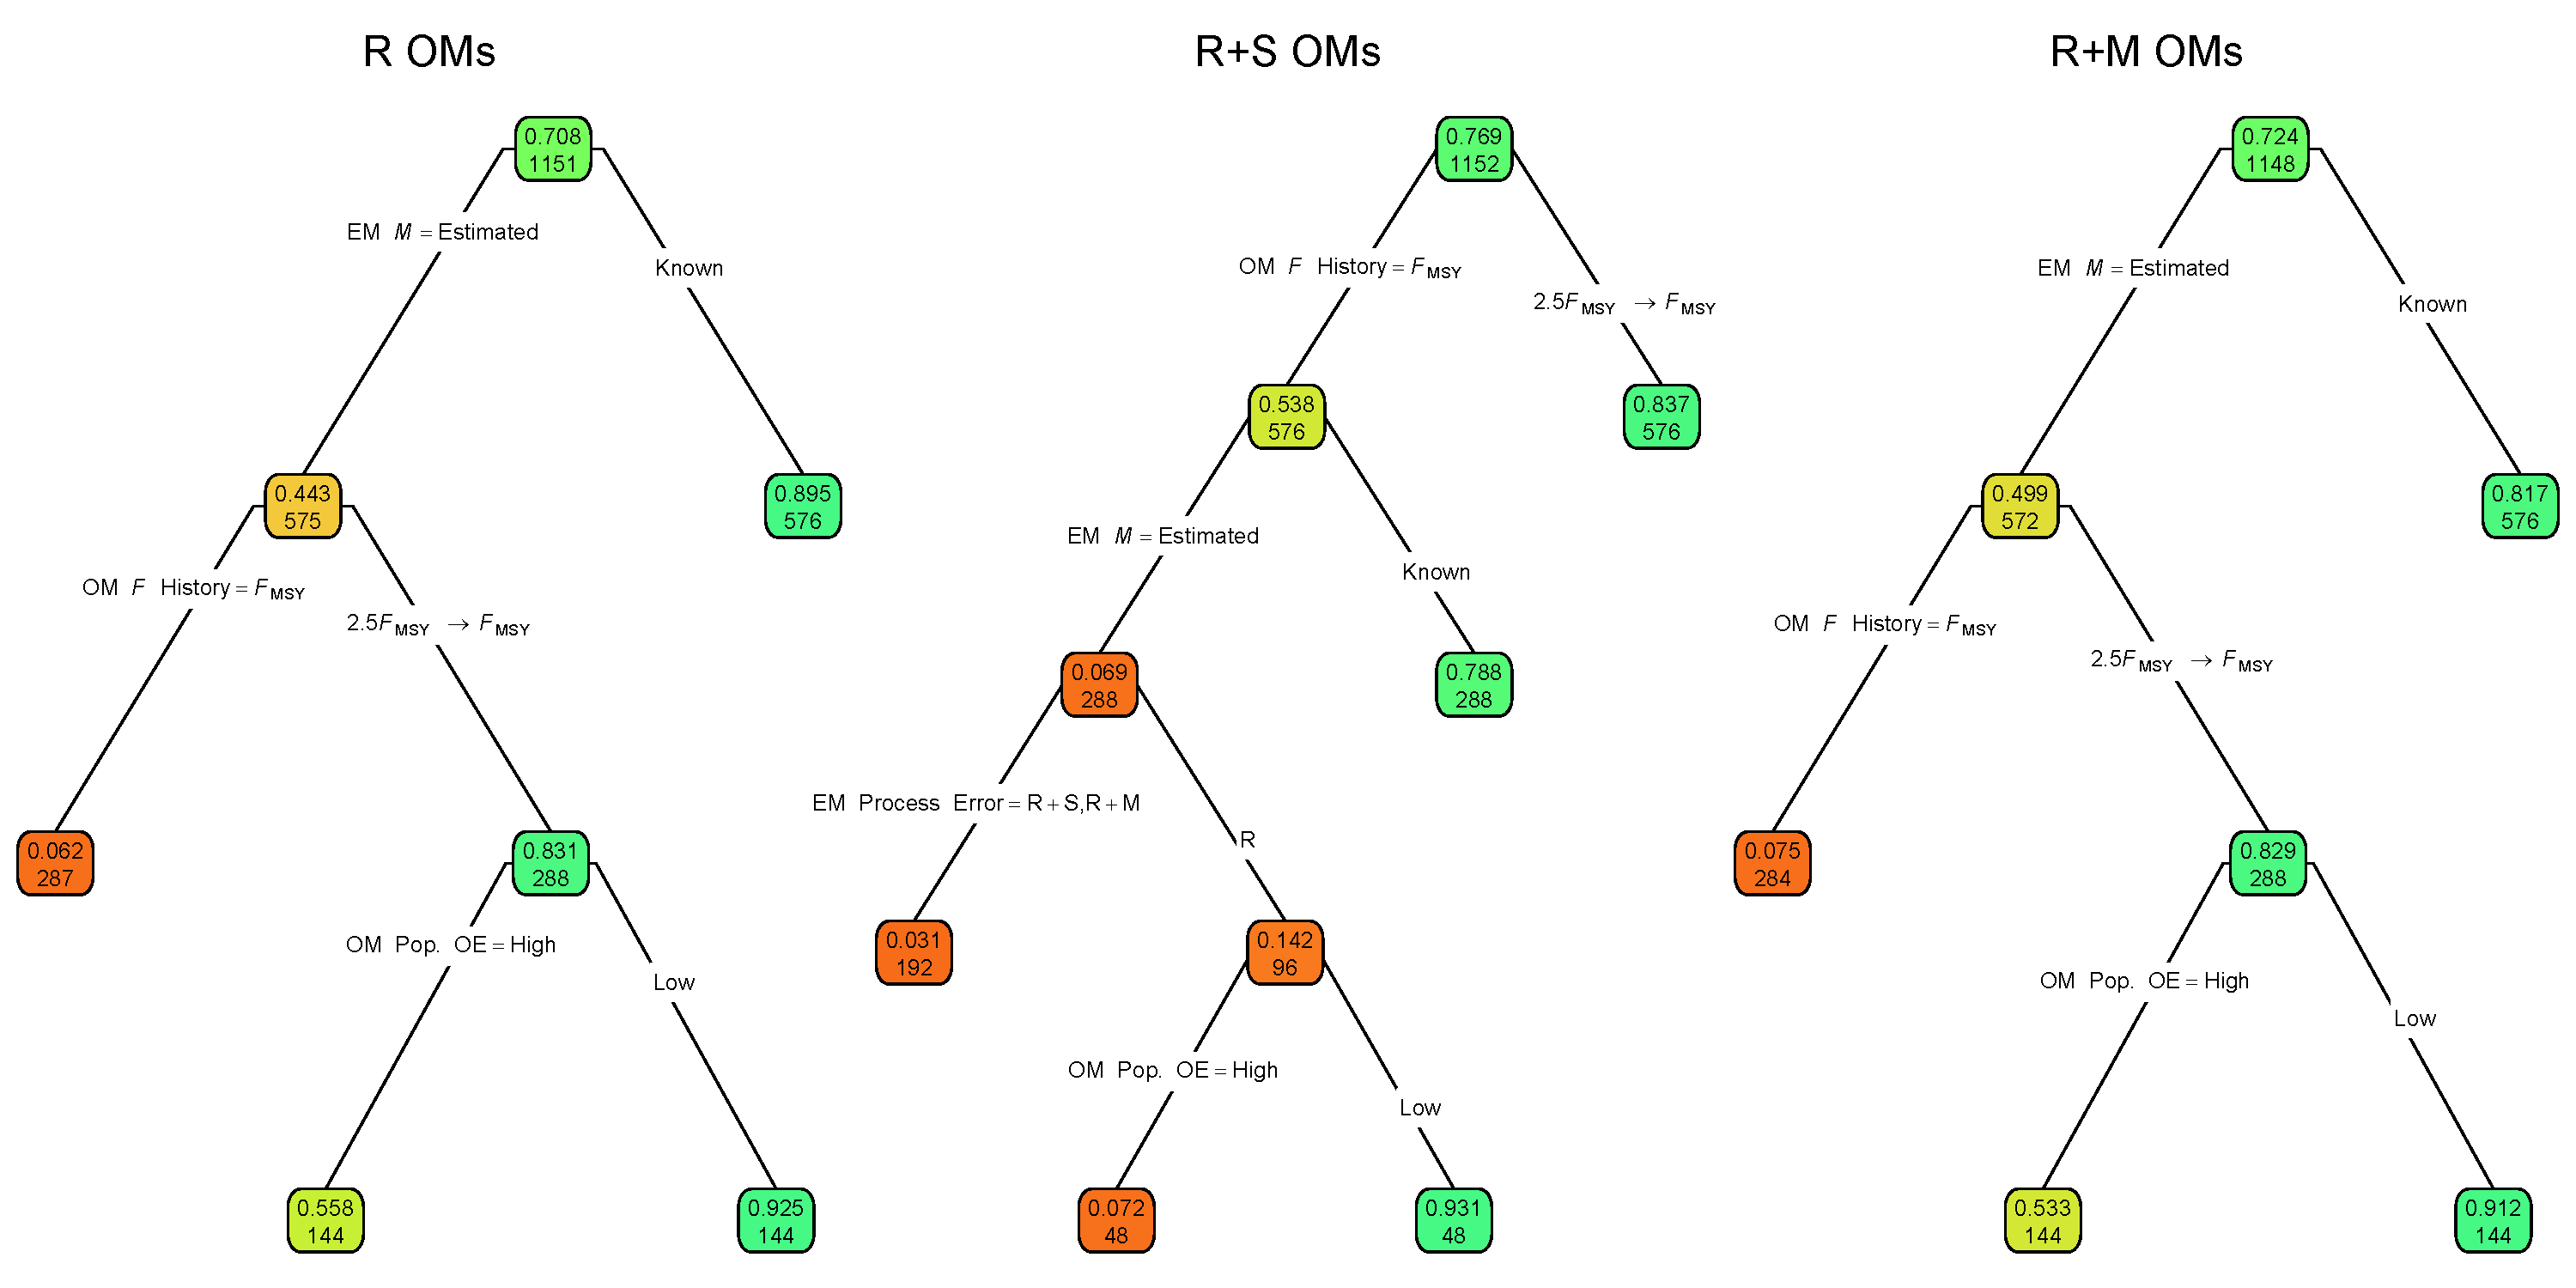
\includegraphics[width = 1.4\textwidth]{term_ssb_corr_regtree_plots}
\end{center}
\caption{\DIFaddFL{Regression trees for the correlation of terminal year SSB estimates and true values. Each node shows the median correlation for the corresponding subset. Lower or higher median correlations are indicated by more red or green polygons, respectively. See Figure \ref{conv_class} caption and Table \ref{factor_table} for further details.}}\label{term_ssb_corr_regtree}
\end{figure}
\end{landscape}
\pagebreak

\begin{landscape}
\begin{figure}
\begin{center}
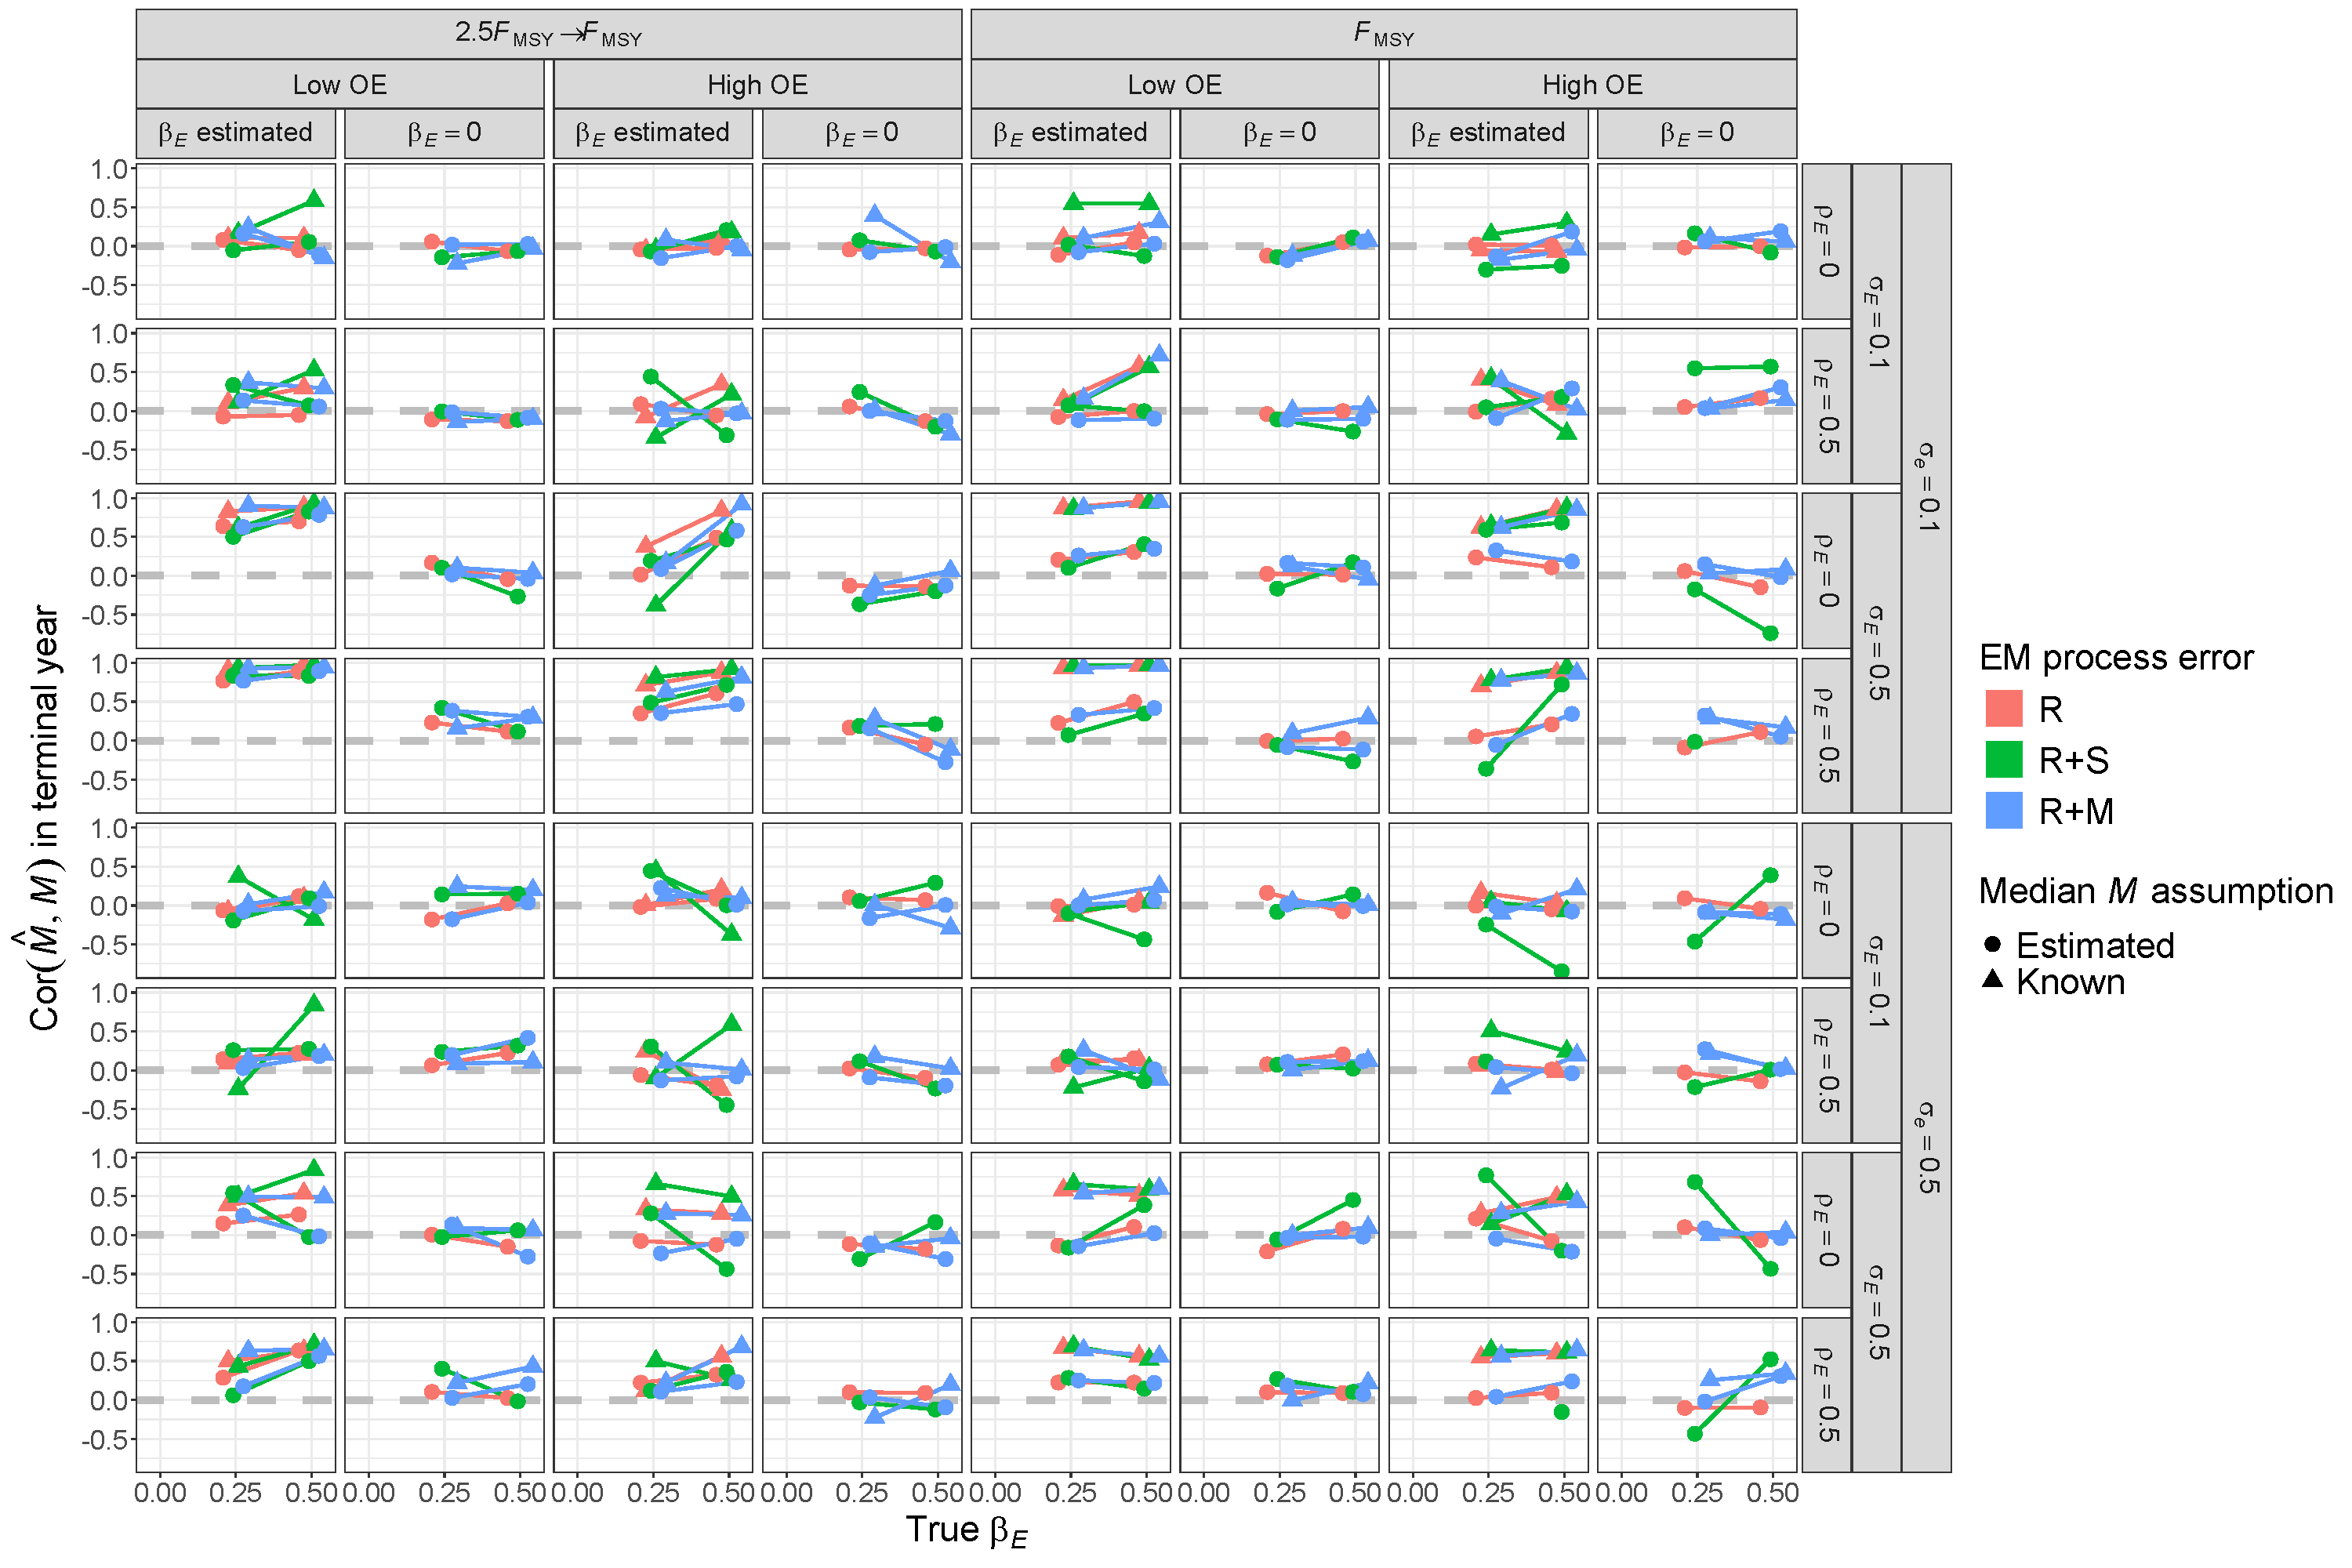
\includegraphics[height = \textheight]{terminal_year_M_corr_Rom}
\end{center}
\caption{\DIFaddFL{For R operating models, correlation of estimates and true values of terminal year $M$ for estimating models with alternative process error assumptions, treatment of covariate effect ($\beta_E = 0$ or estimated), and treatment of median $M$ parameter ($\beta_M$ estimated or known).}}\label{terminal_M_corr_Rom}
\end{figure}
\end{landscape}

\begin{landscape}
\begin{figure}
\begin{center}
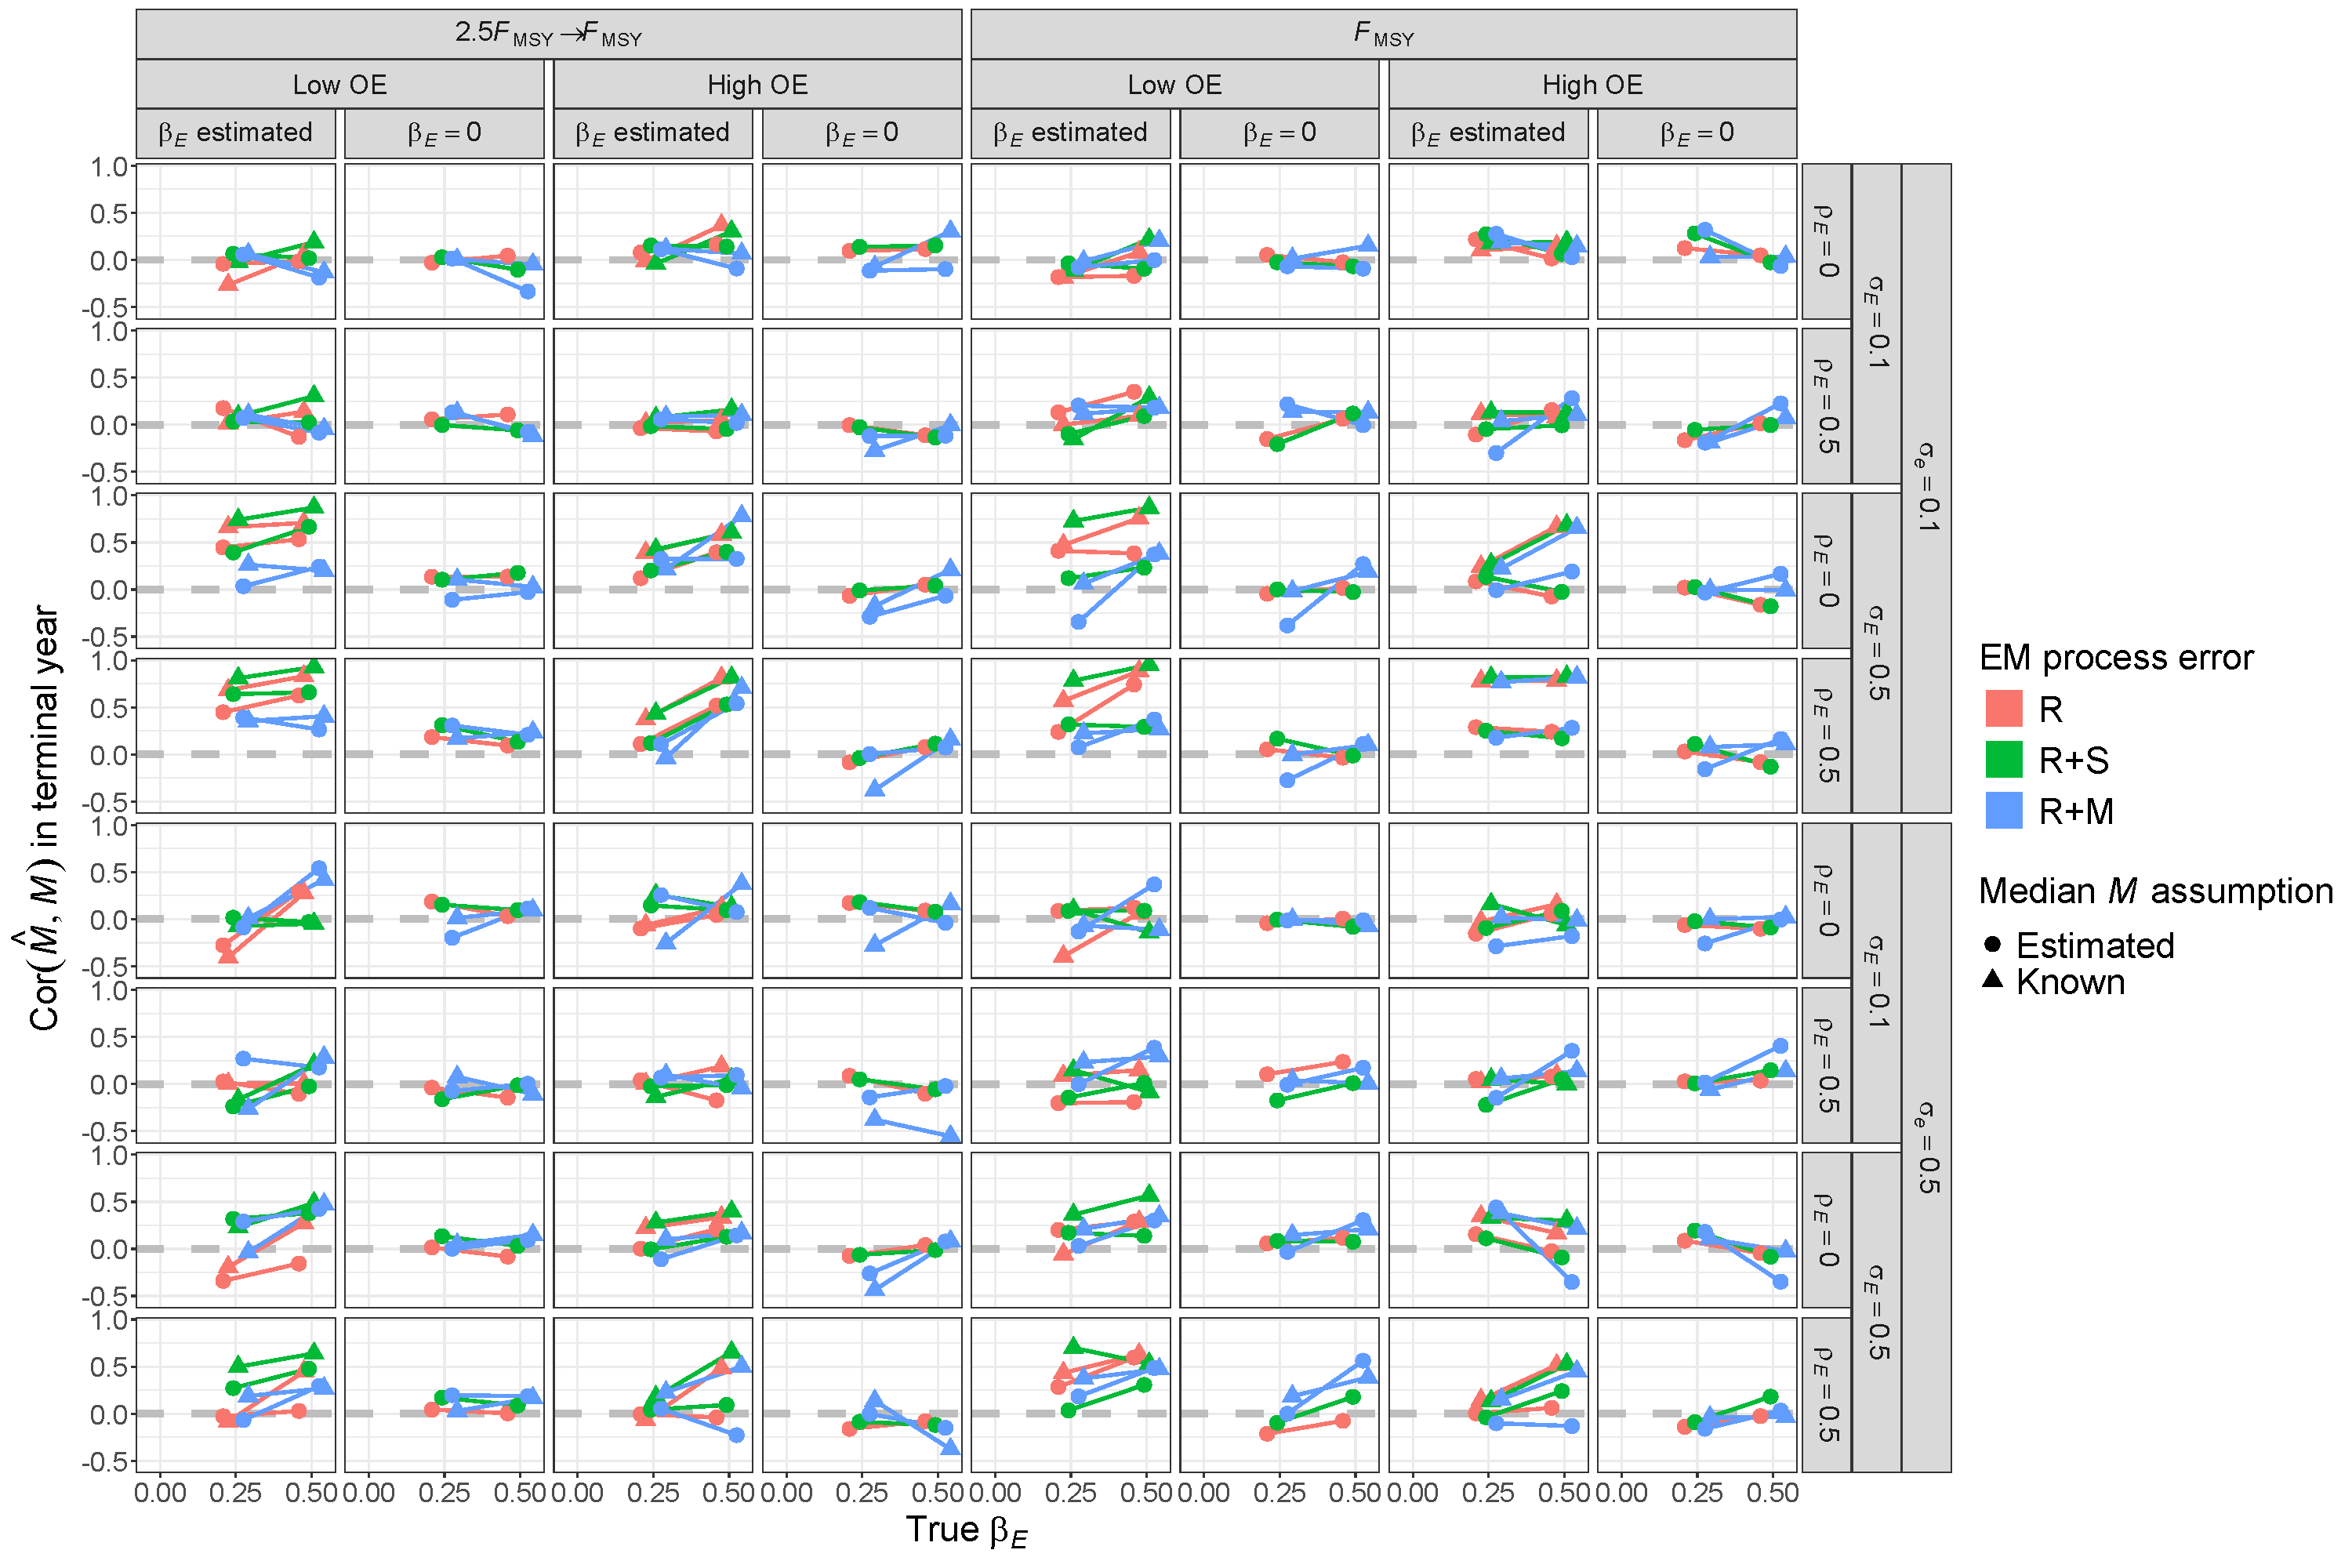
\includegraphics[height = \textheight]{terminal_year_M_corr_RSom}
\end{center}
\caption{\DIFaddFL{For R+S operating models, correlation of estimates and true values of terminal year $M$ for estimating models with alternative process error assumptions, treatment of covariate effect ($\beta_E = 0$ or estimated), and treatment of median $M$ parameter ($\beta_M$ estimated or known).}}\label{terminal_M_corr_RSom}
\end{figure}
\end{landscape}

\begin{landscape}
\begin{figure}
\begin{center}
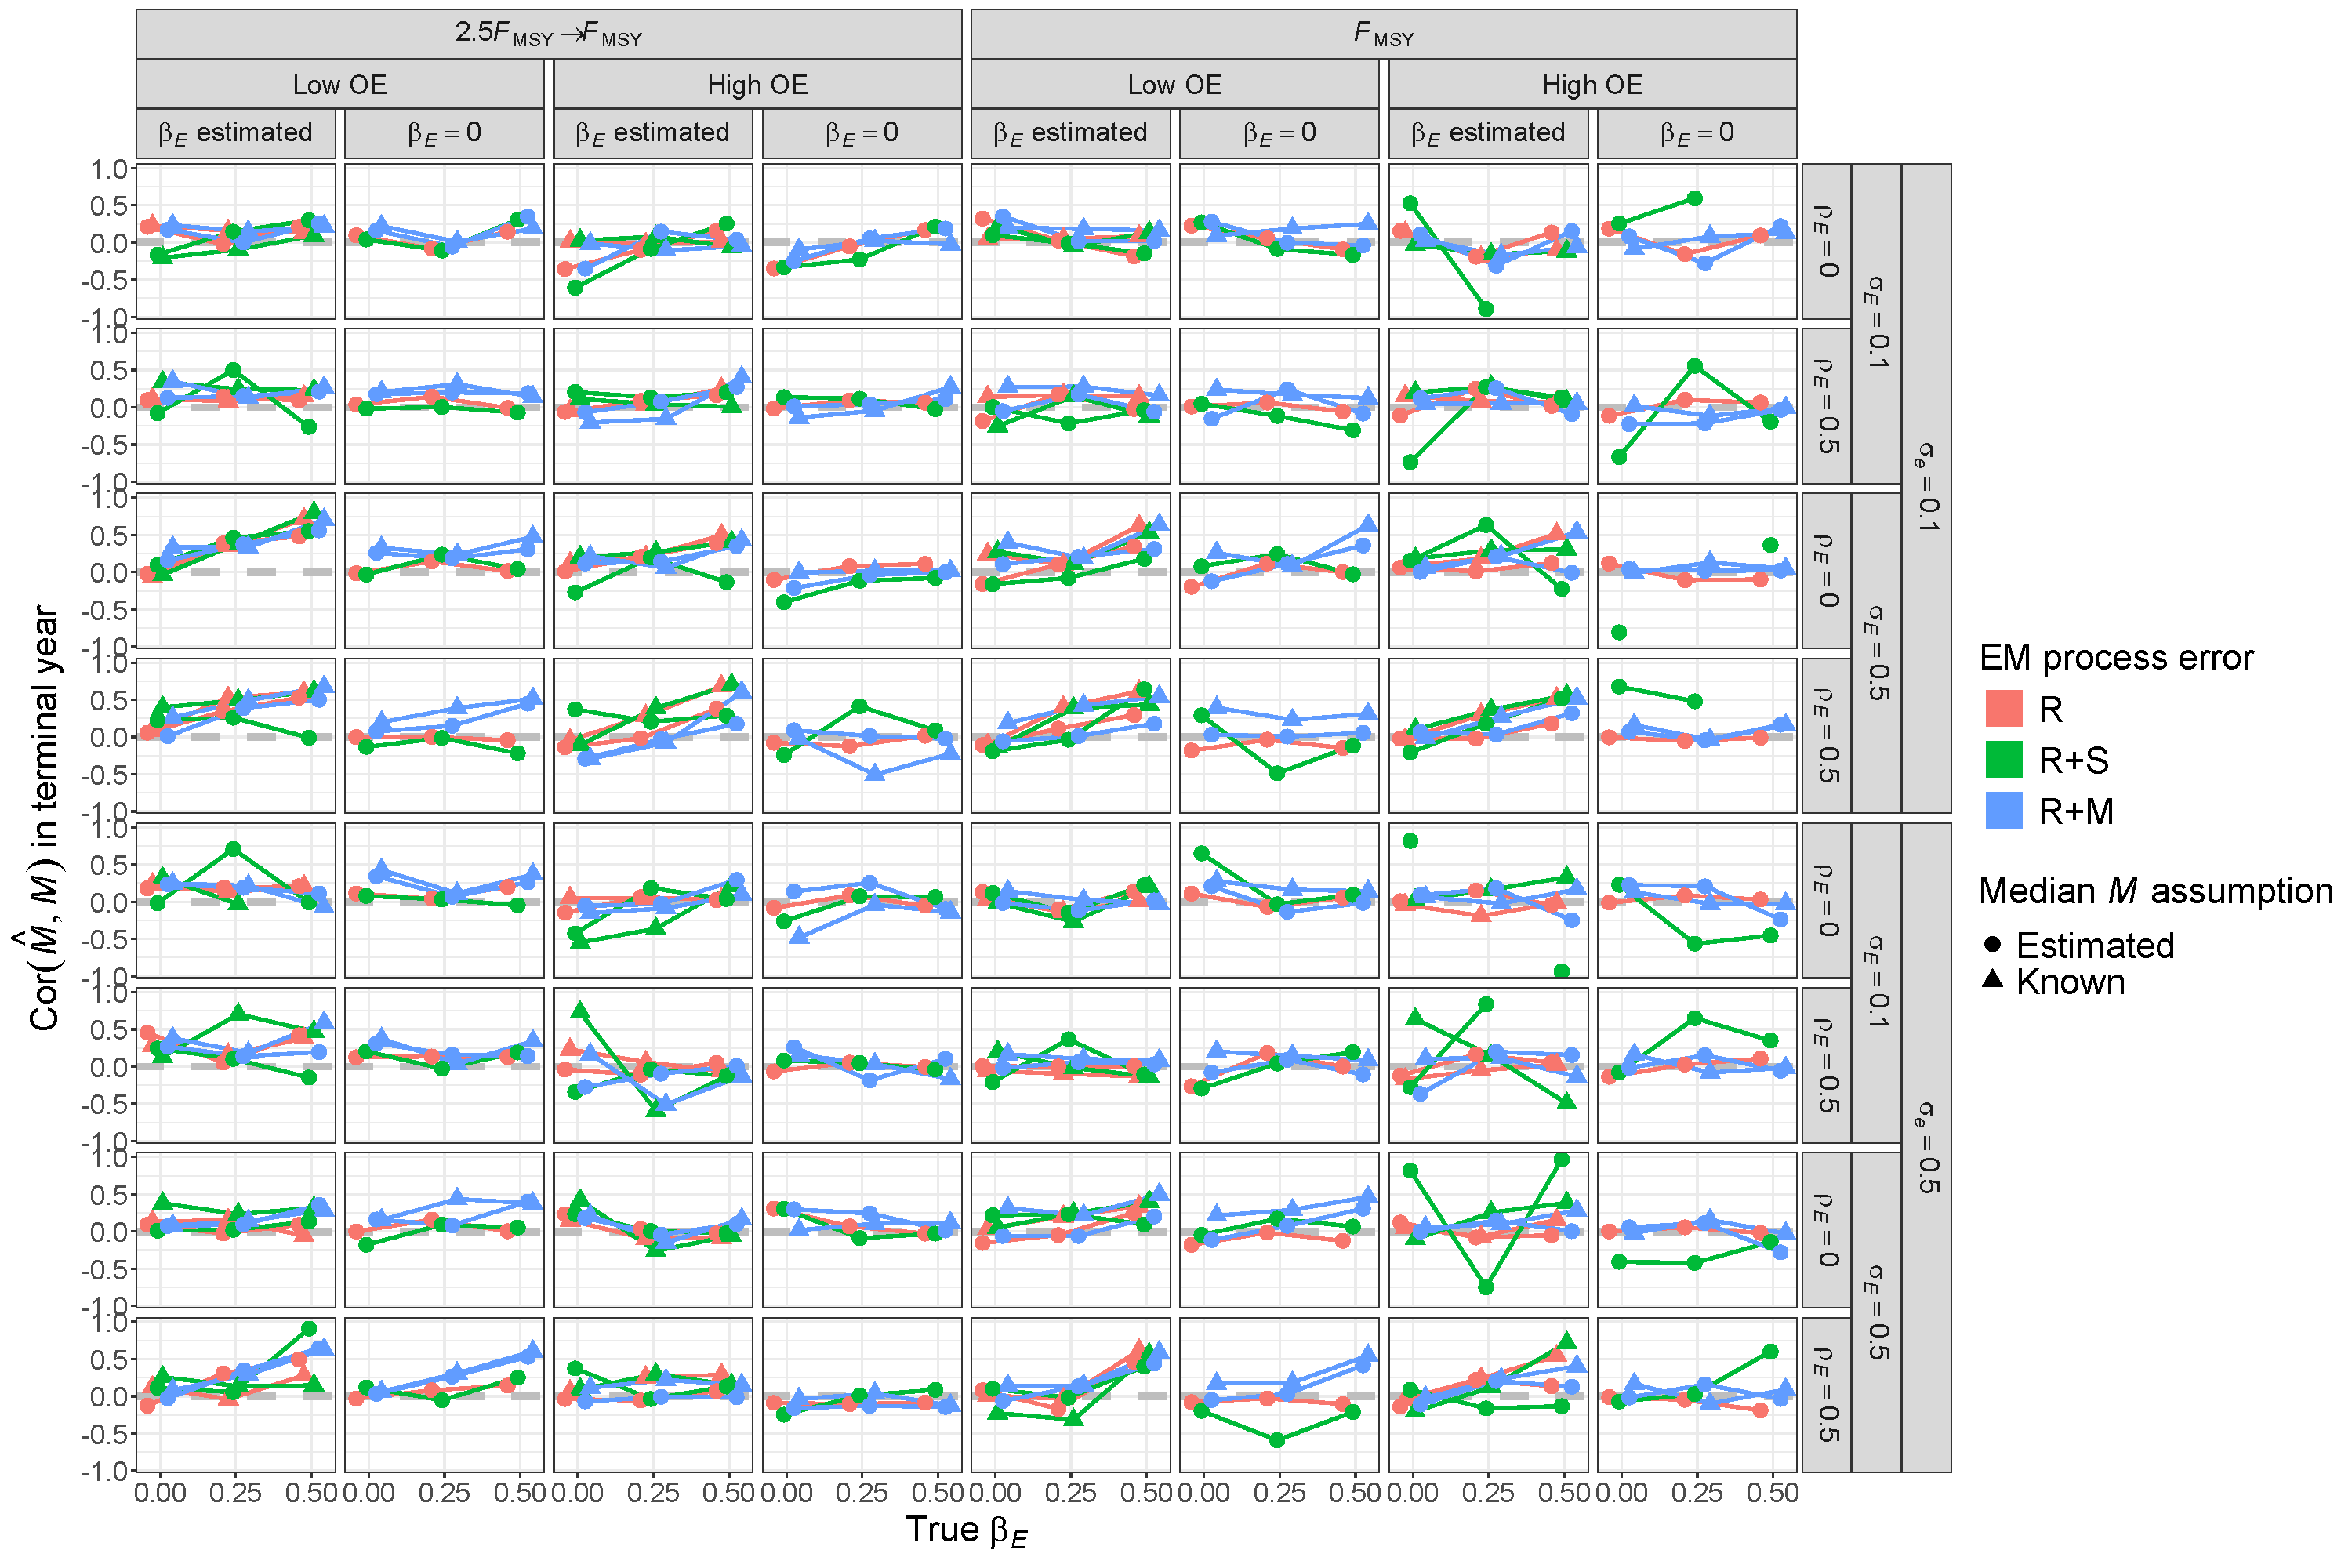
\includegraphics[height = \textheight]{terminal_year_M_corr_RMom}
\end{center}
\caption{\DIFaddFL{For R+M operating models, correlation of estimates and true vales of terminal year $M$ for estimating models with alternative process error assumptions, treatment of covariate effect ($\beta_E = 0$ or estimated), and treatment of median $M$ parameter ($\beta_M$ estimated or known).}}\label{terminal_M_corr_RMom}
\end{figure}
\end{landscape}

\begin{landscape}
\begin{figure}
\begin{center}
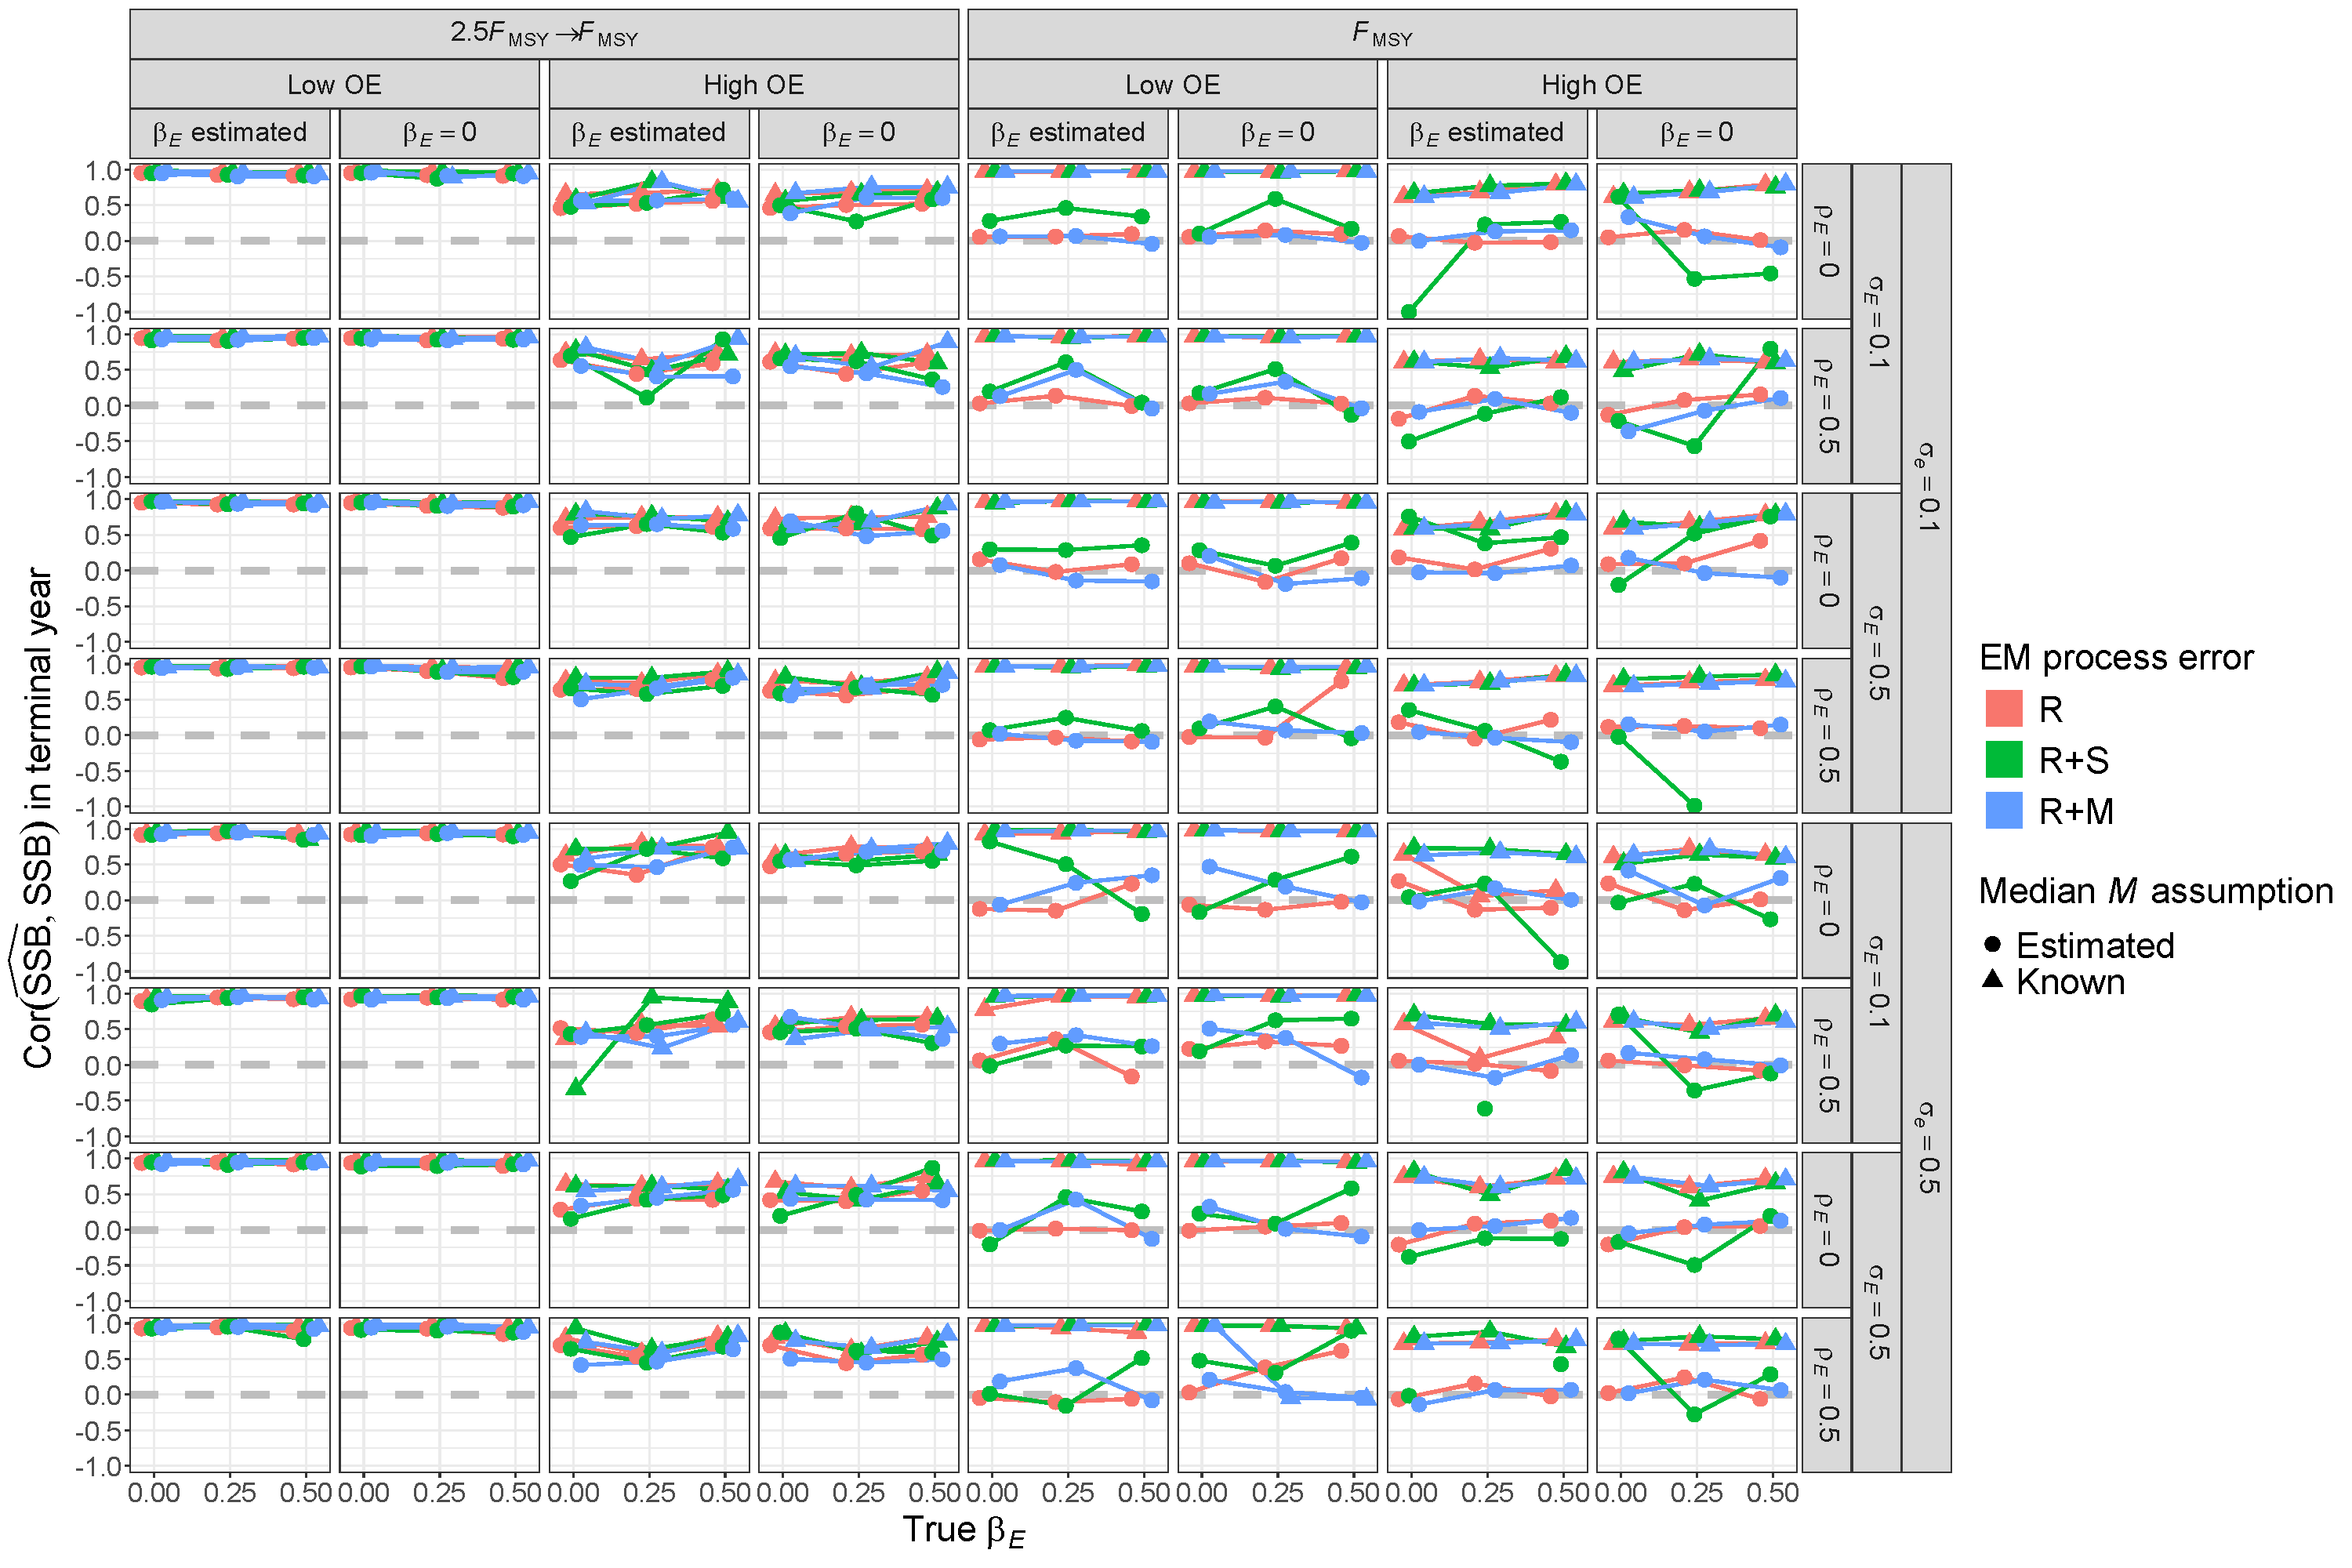
\includegraphics[height = \textheight]{terminal_year_ssb_corr_Rom}
\end{center}
\caption{\DIFaddFL{For R operating models, correlation of estimates and true values of terminal year SSB for estimating models with alternative process error assumptions, treatment of covariate effect ($\beta_E = 0$ or estimated), and treatment of median $M$ parameter ($\beta_M$ estimated or known).}}\label{terminal_ssb_corr_Rom}
\end{figure}
\end{landscape}

\begin{landscape}
\begin{figure}
\begin{center}
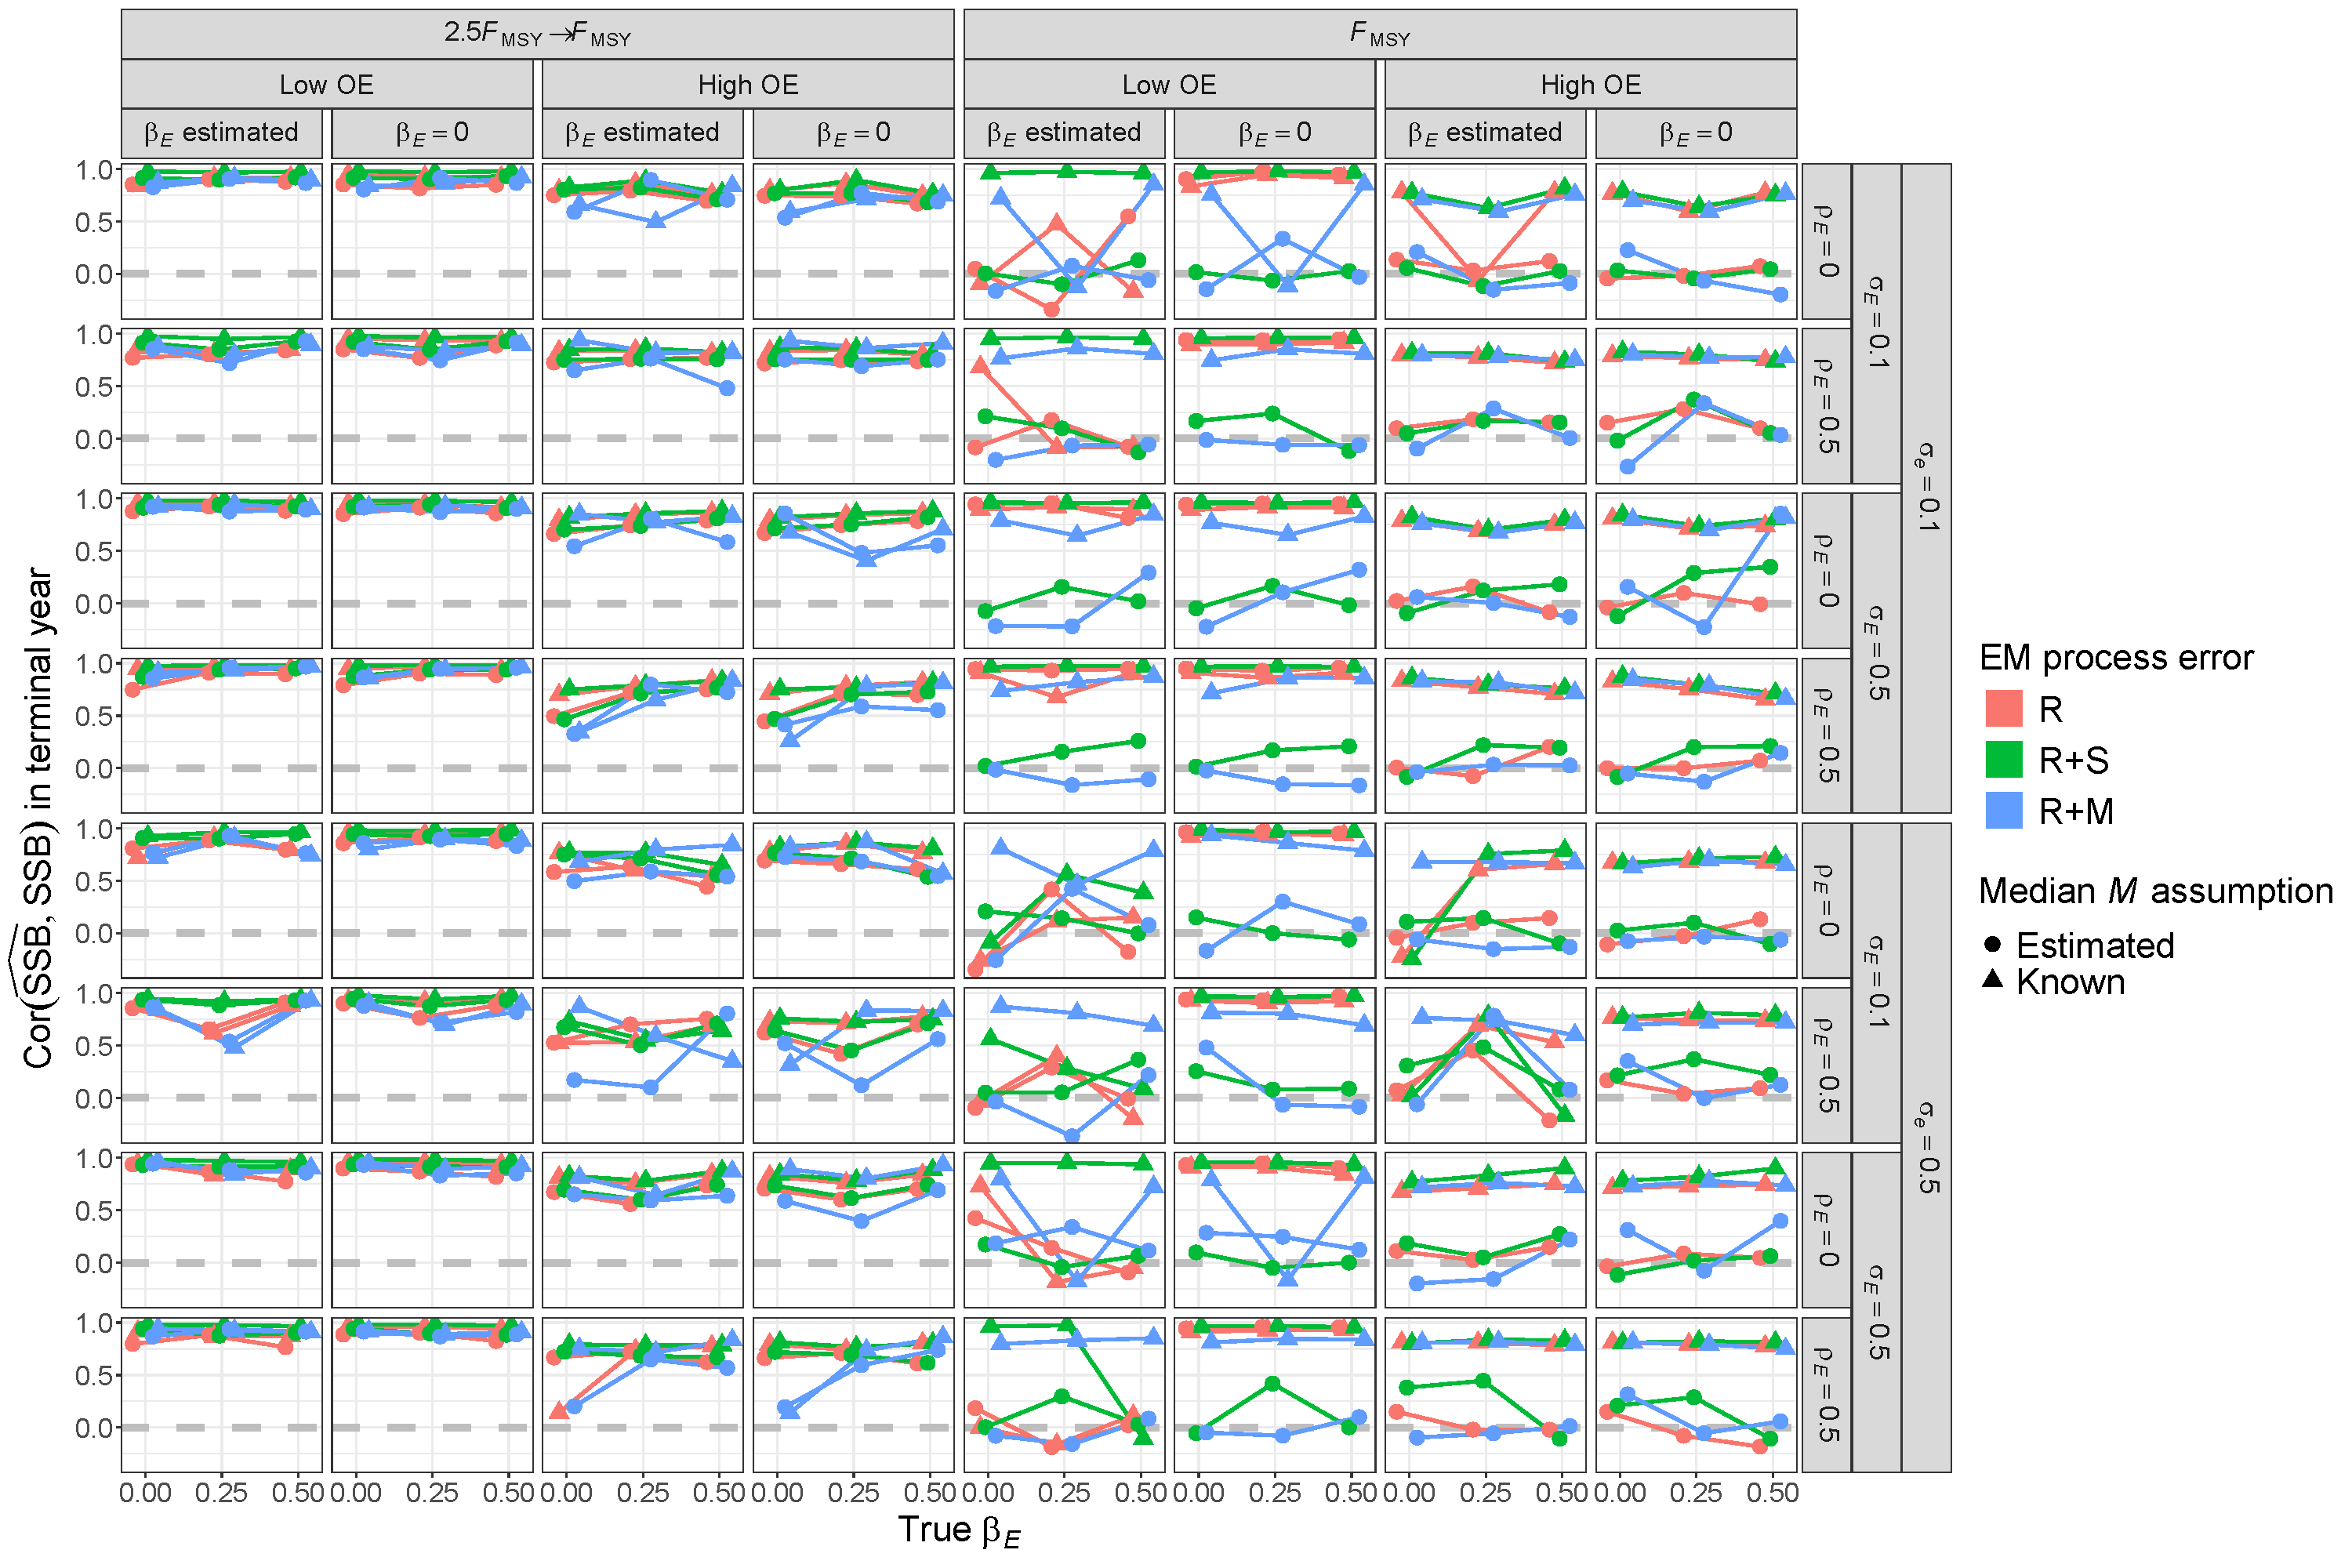
\includegraphics[height = \textheight]{terminal_year_ssb_corr_RSom}
\end{center}
\caption{\DIFaddFL{For R+S operating models, correlation of estimates and true values of terminal year SSB for estimating models with alternative process error assumptions, treatment of covariate effect ($\beta_E = 0$ or estimated), and treatment of median $M$ parameter ($\beta_M$ estimated or known).}}\label{terminal_ssb_corr_RSom}
\end{figure}
\end{landscape}

\begin{landscape}
\begin{figure}
\begin{center}
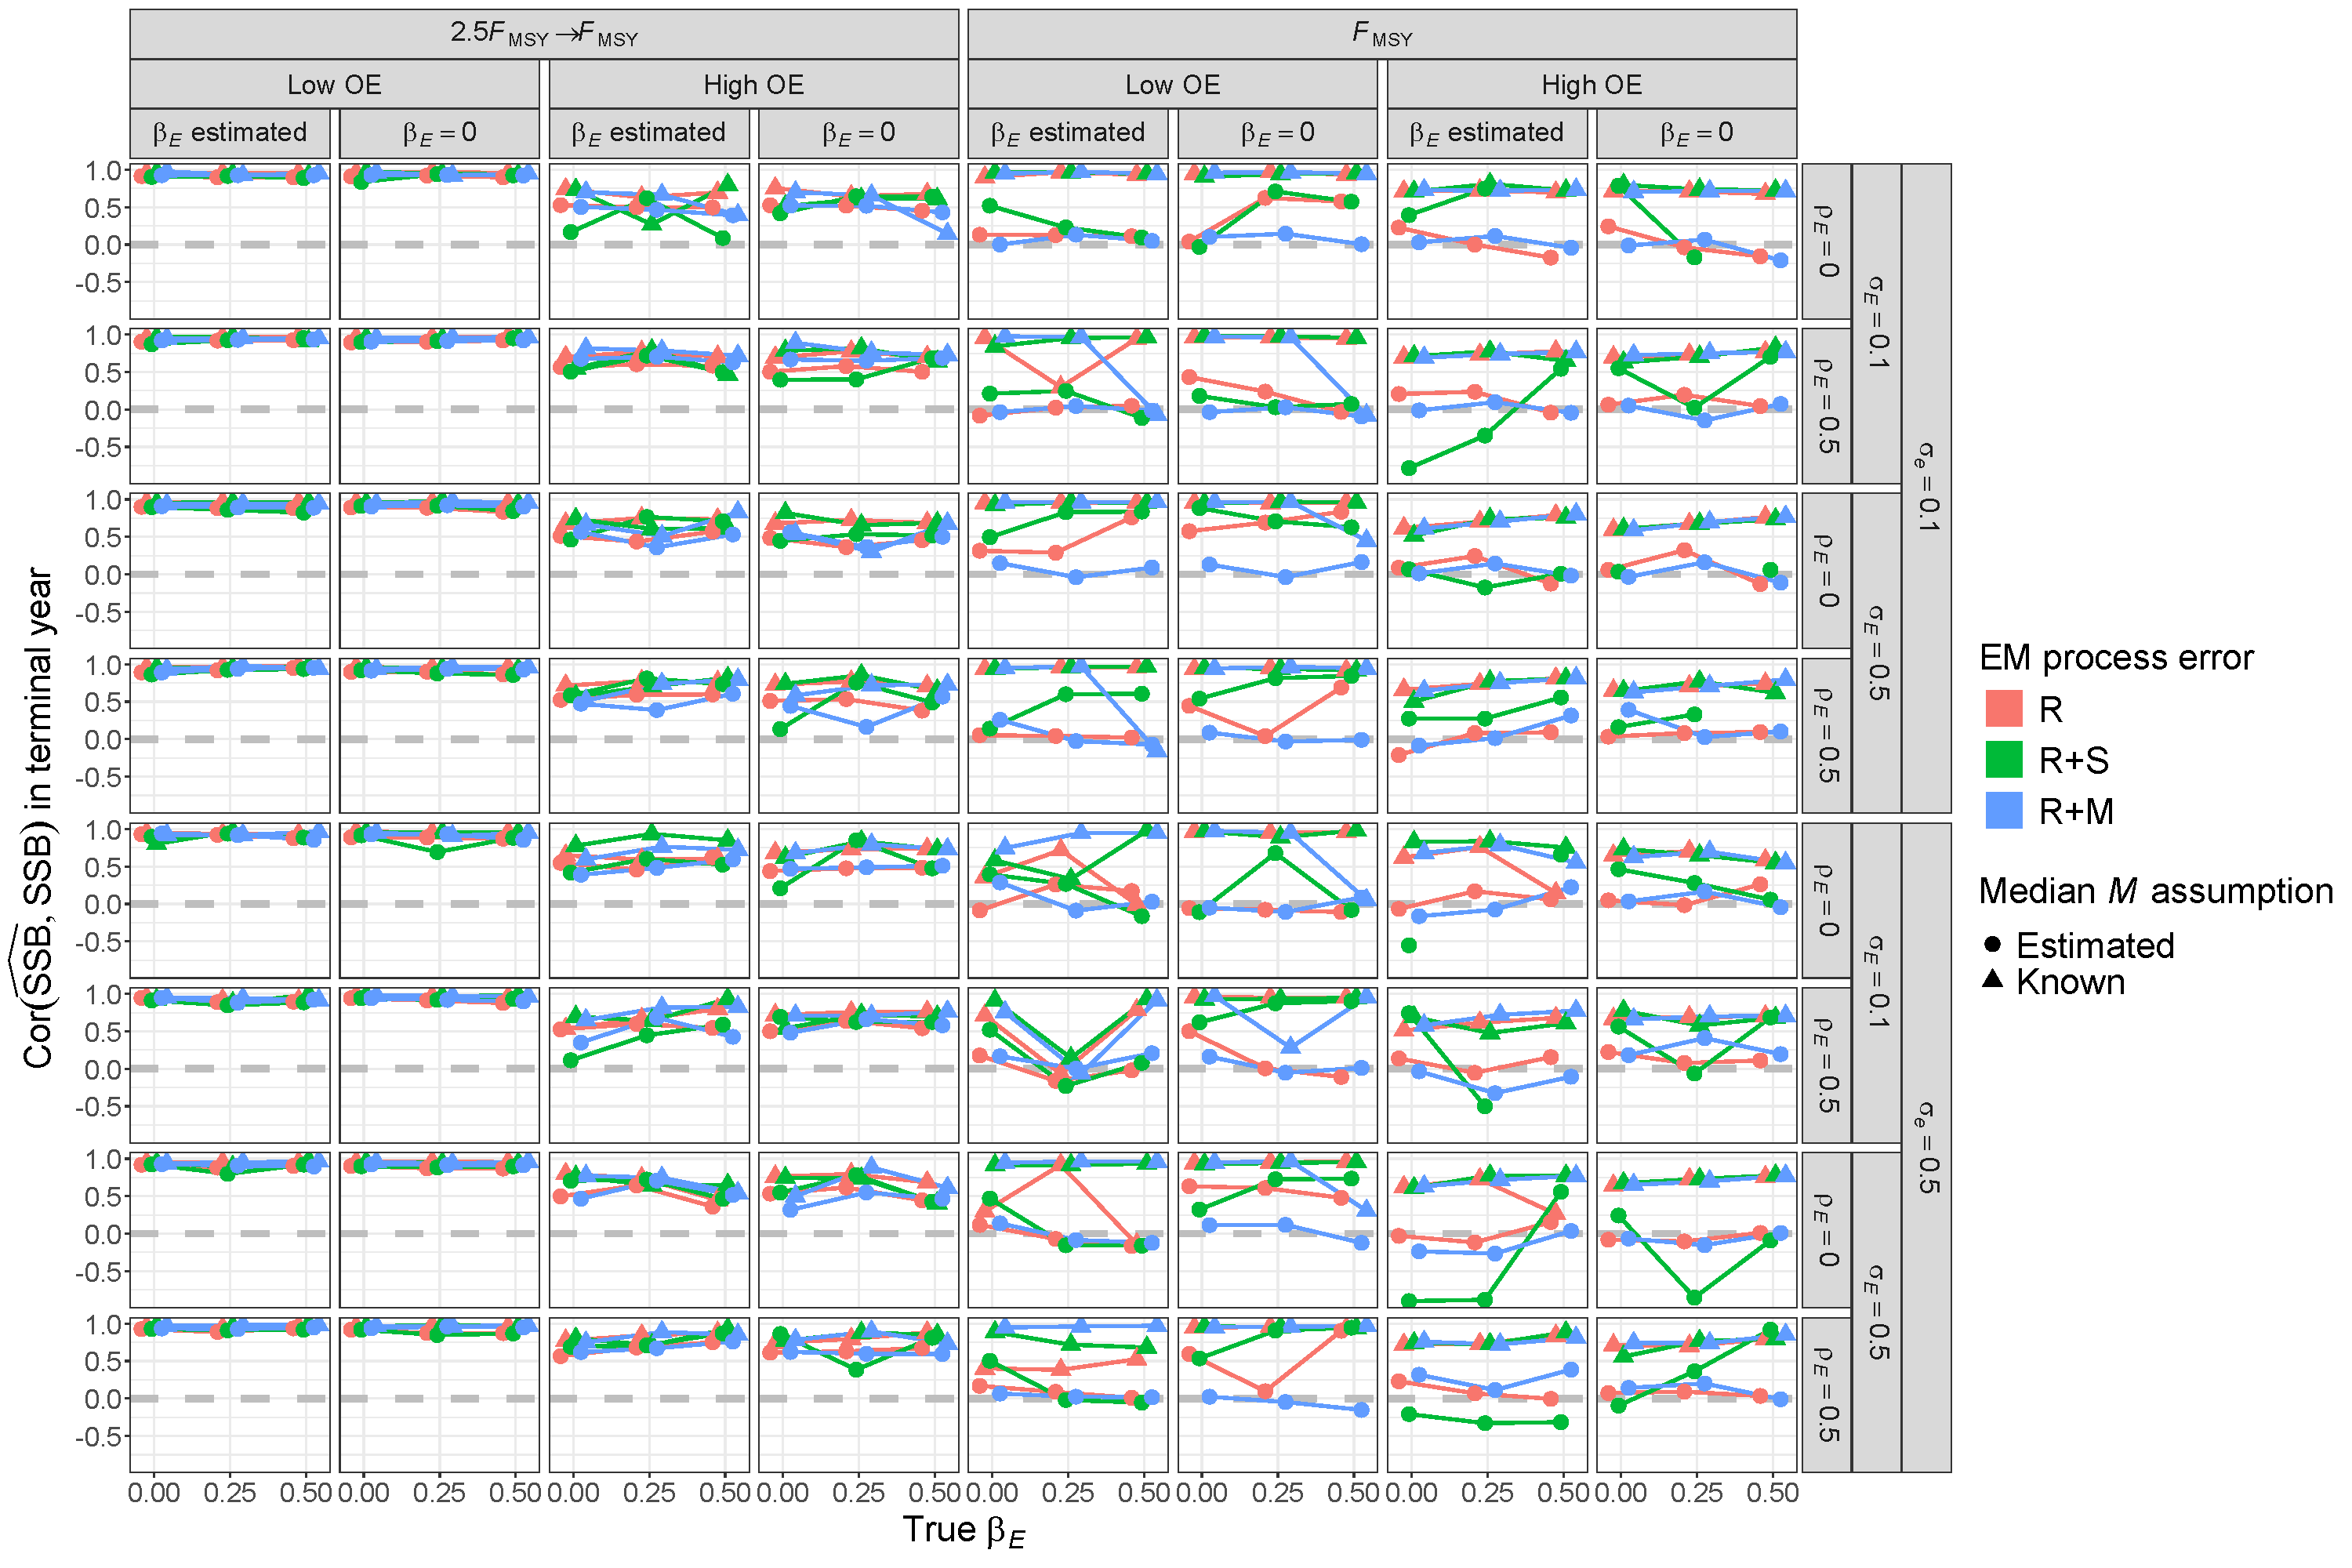
\includegraphics[height = \textheight]{terminal_year_ssb_corr_RMom}
\end{center}
\caption{\DIFaddFL{For R+M operating models, correlation of estimates and true vales of terminal year SSB for estimating models with alternative process error assumptions, treatment of covariate effect ($\beta_E = 0$ or estimated), and treatment of median $M$ parameter ($\beta_M$ estimated or known).}}\label{terminal_ssb_corr_RMom}
\end{figure}
\end{landscape}

\begin{landscape}
\begin{figure}
\begin{center}
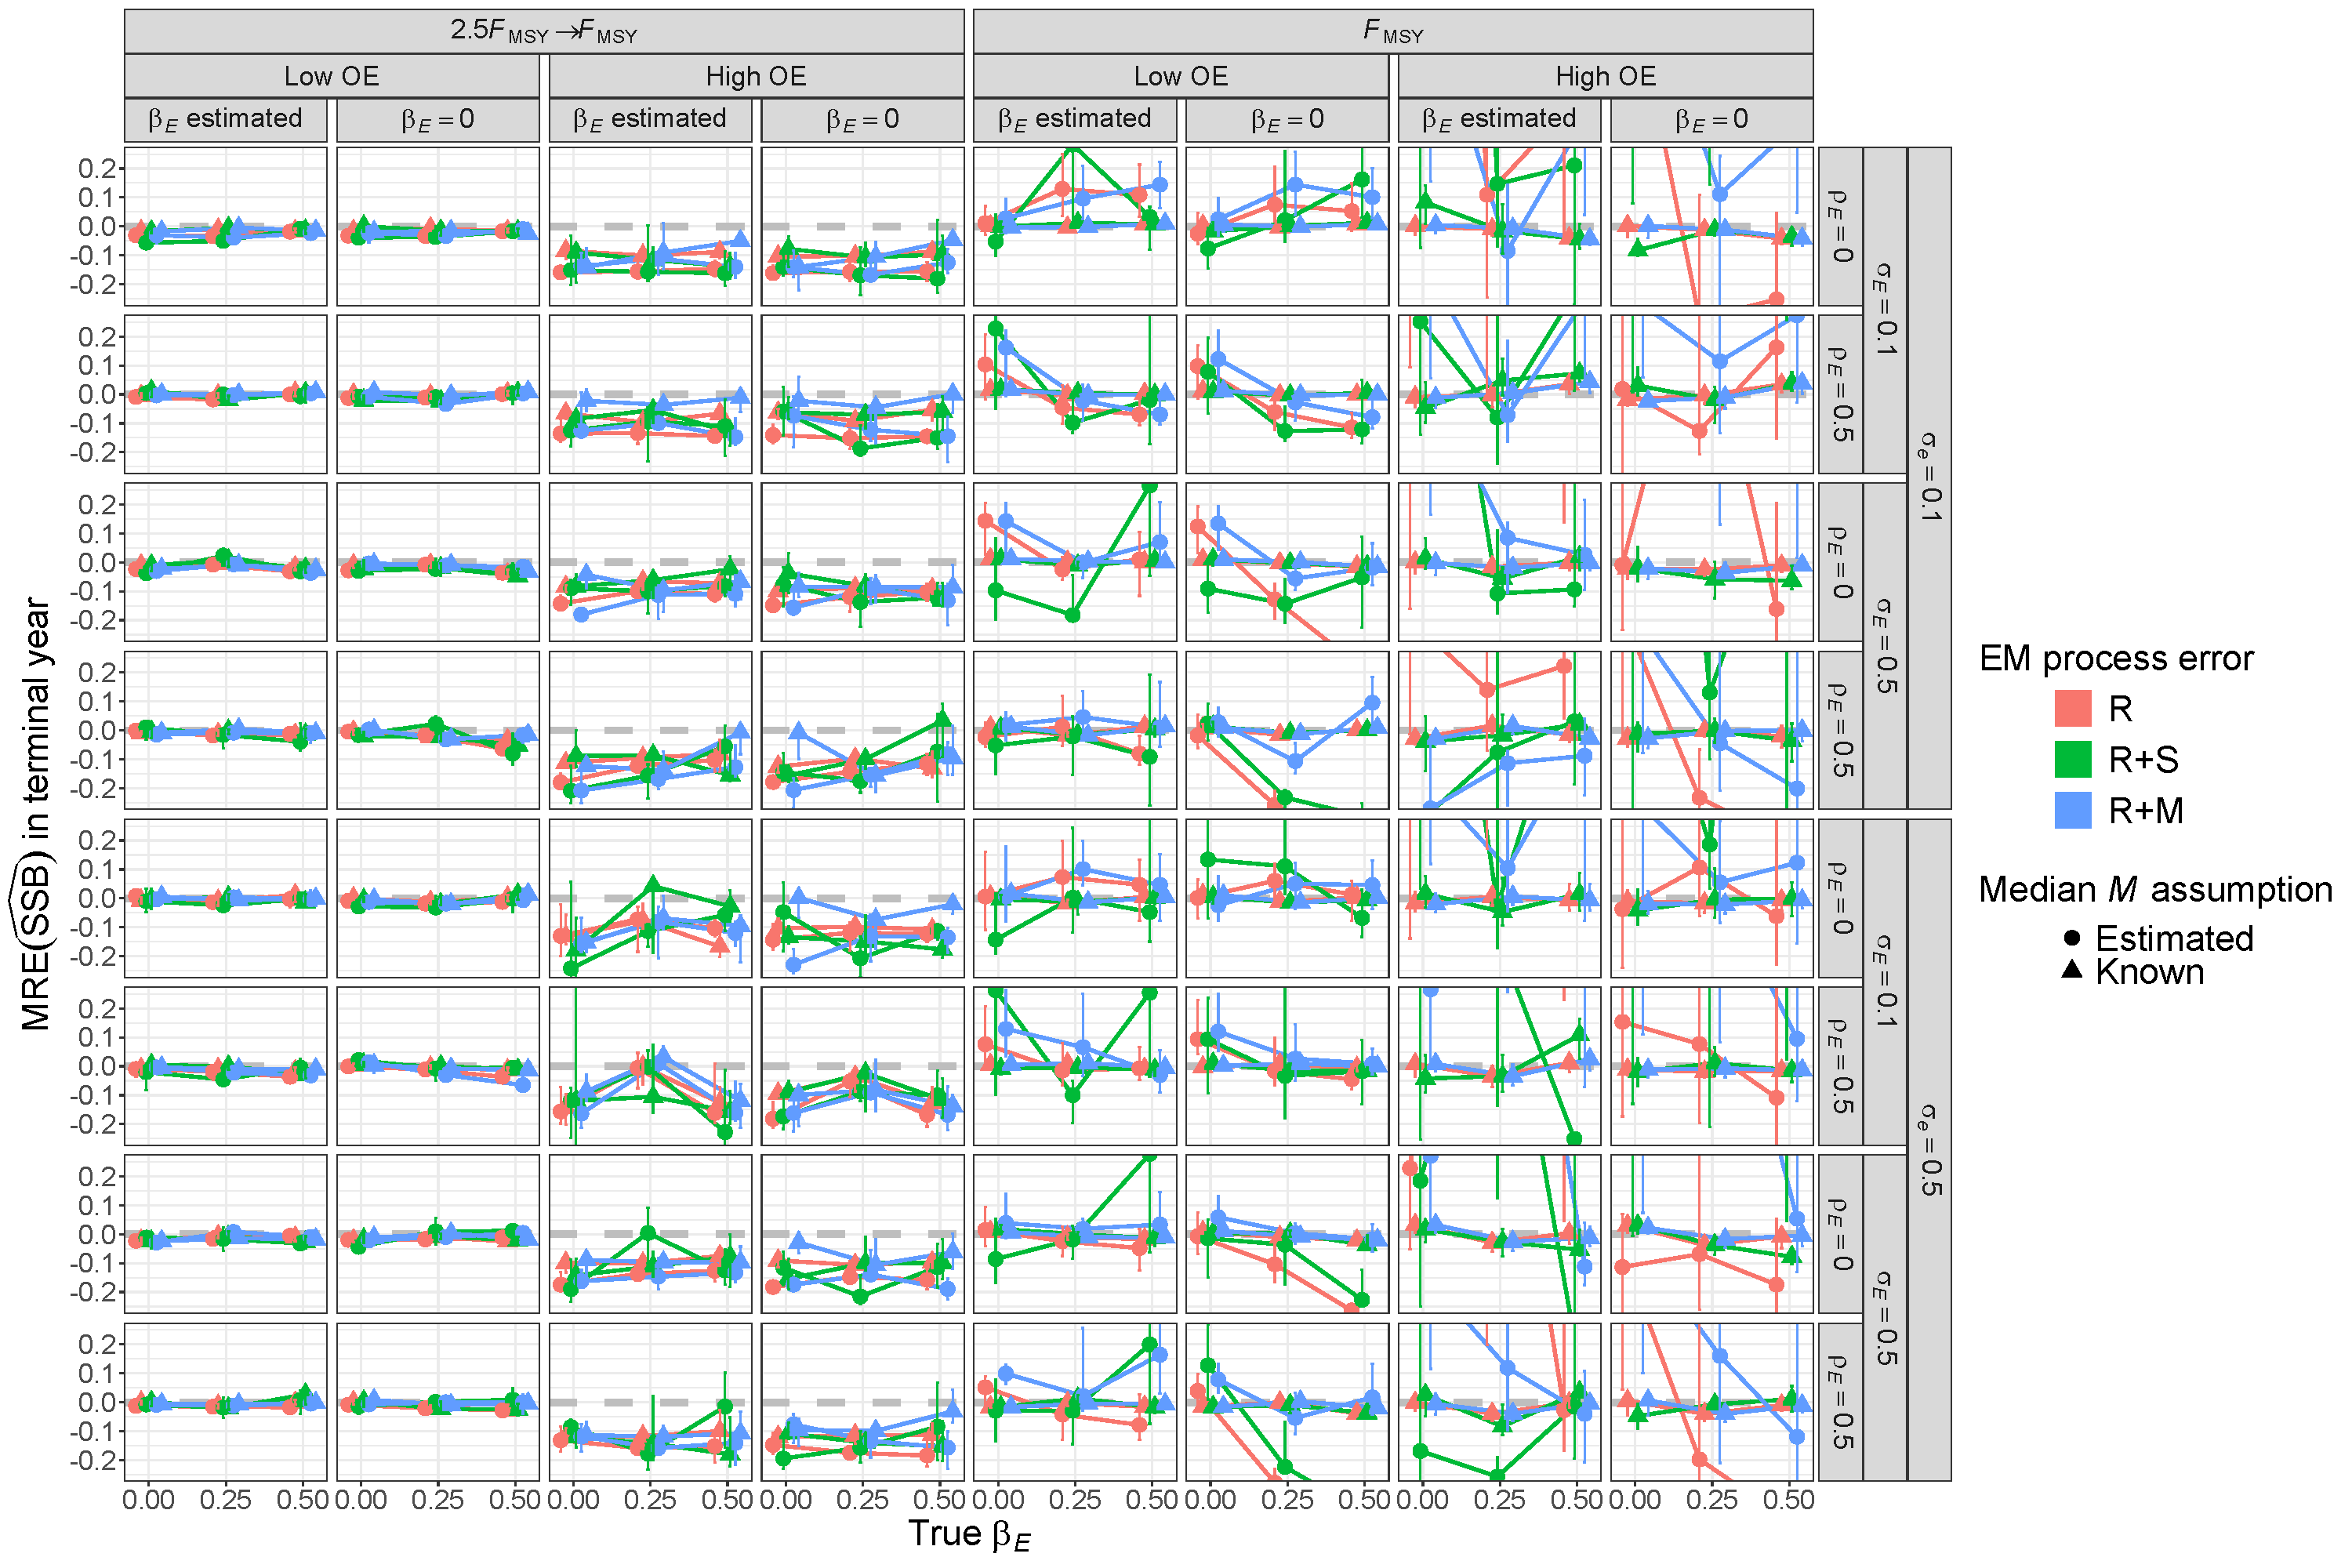
\includegraphics[height = \textheight]{terminal_year_ssb_bias_Rom}
\end{center}
\caption{\DIFaddFL{For R operating models, median relative error (MRE) of estimates of SSB in the terminal year for estimating models with alternative process error assumptions, treatment of covariate effect ($\beta_E = 0$ or estimated), and treatment of median $M$ parameter ($\beta_M$ estimated or known).}}\label{terminal_ssb_bias_Rom}
\end{figure}
\end{landscape}

\begin{landscape}
\begin{figure}
\begin{center}
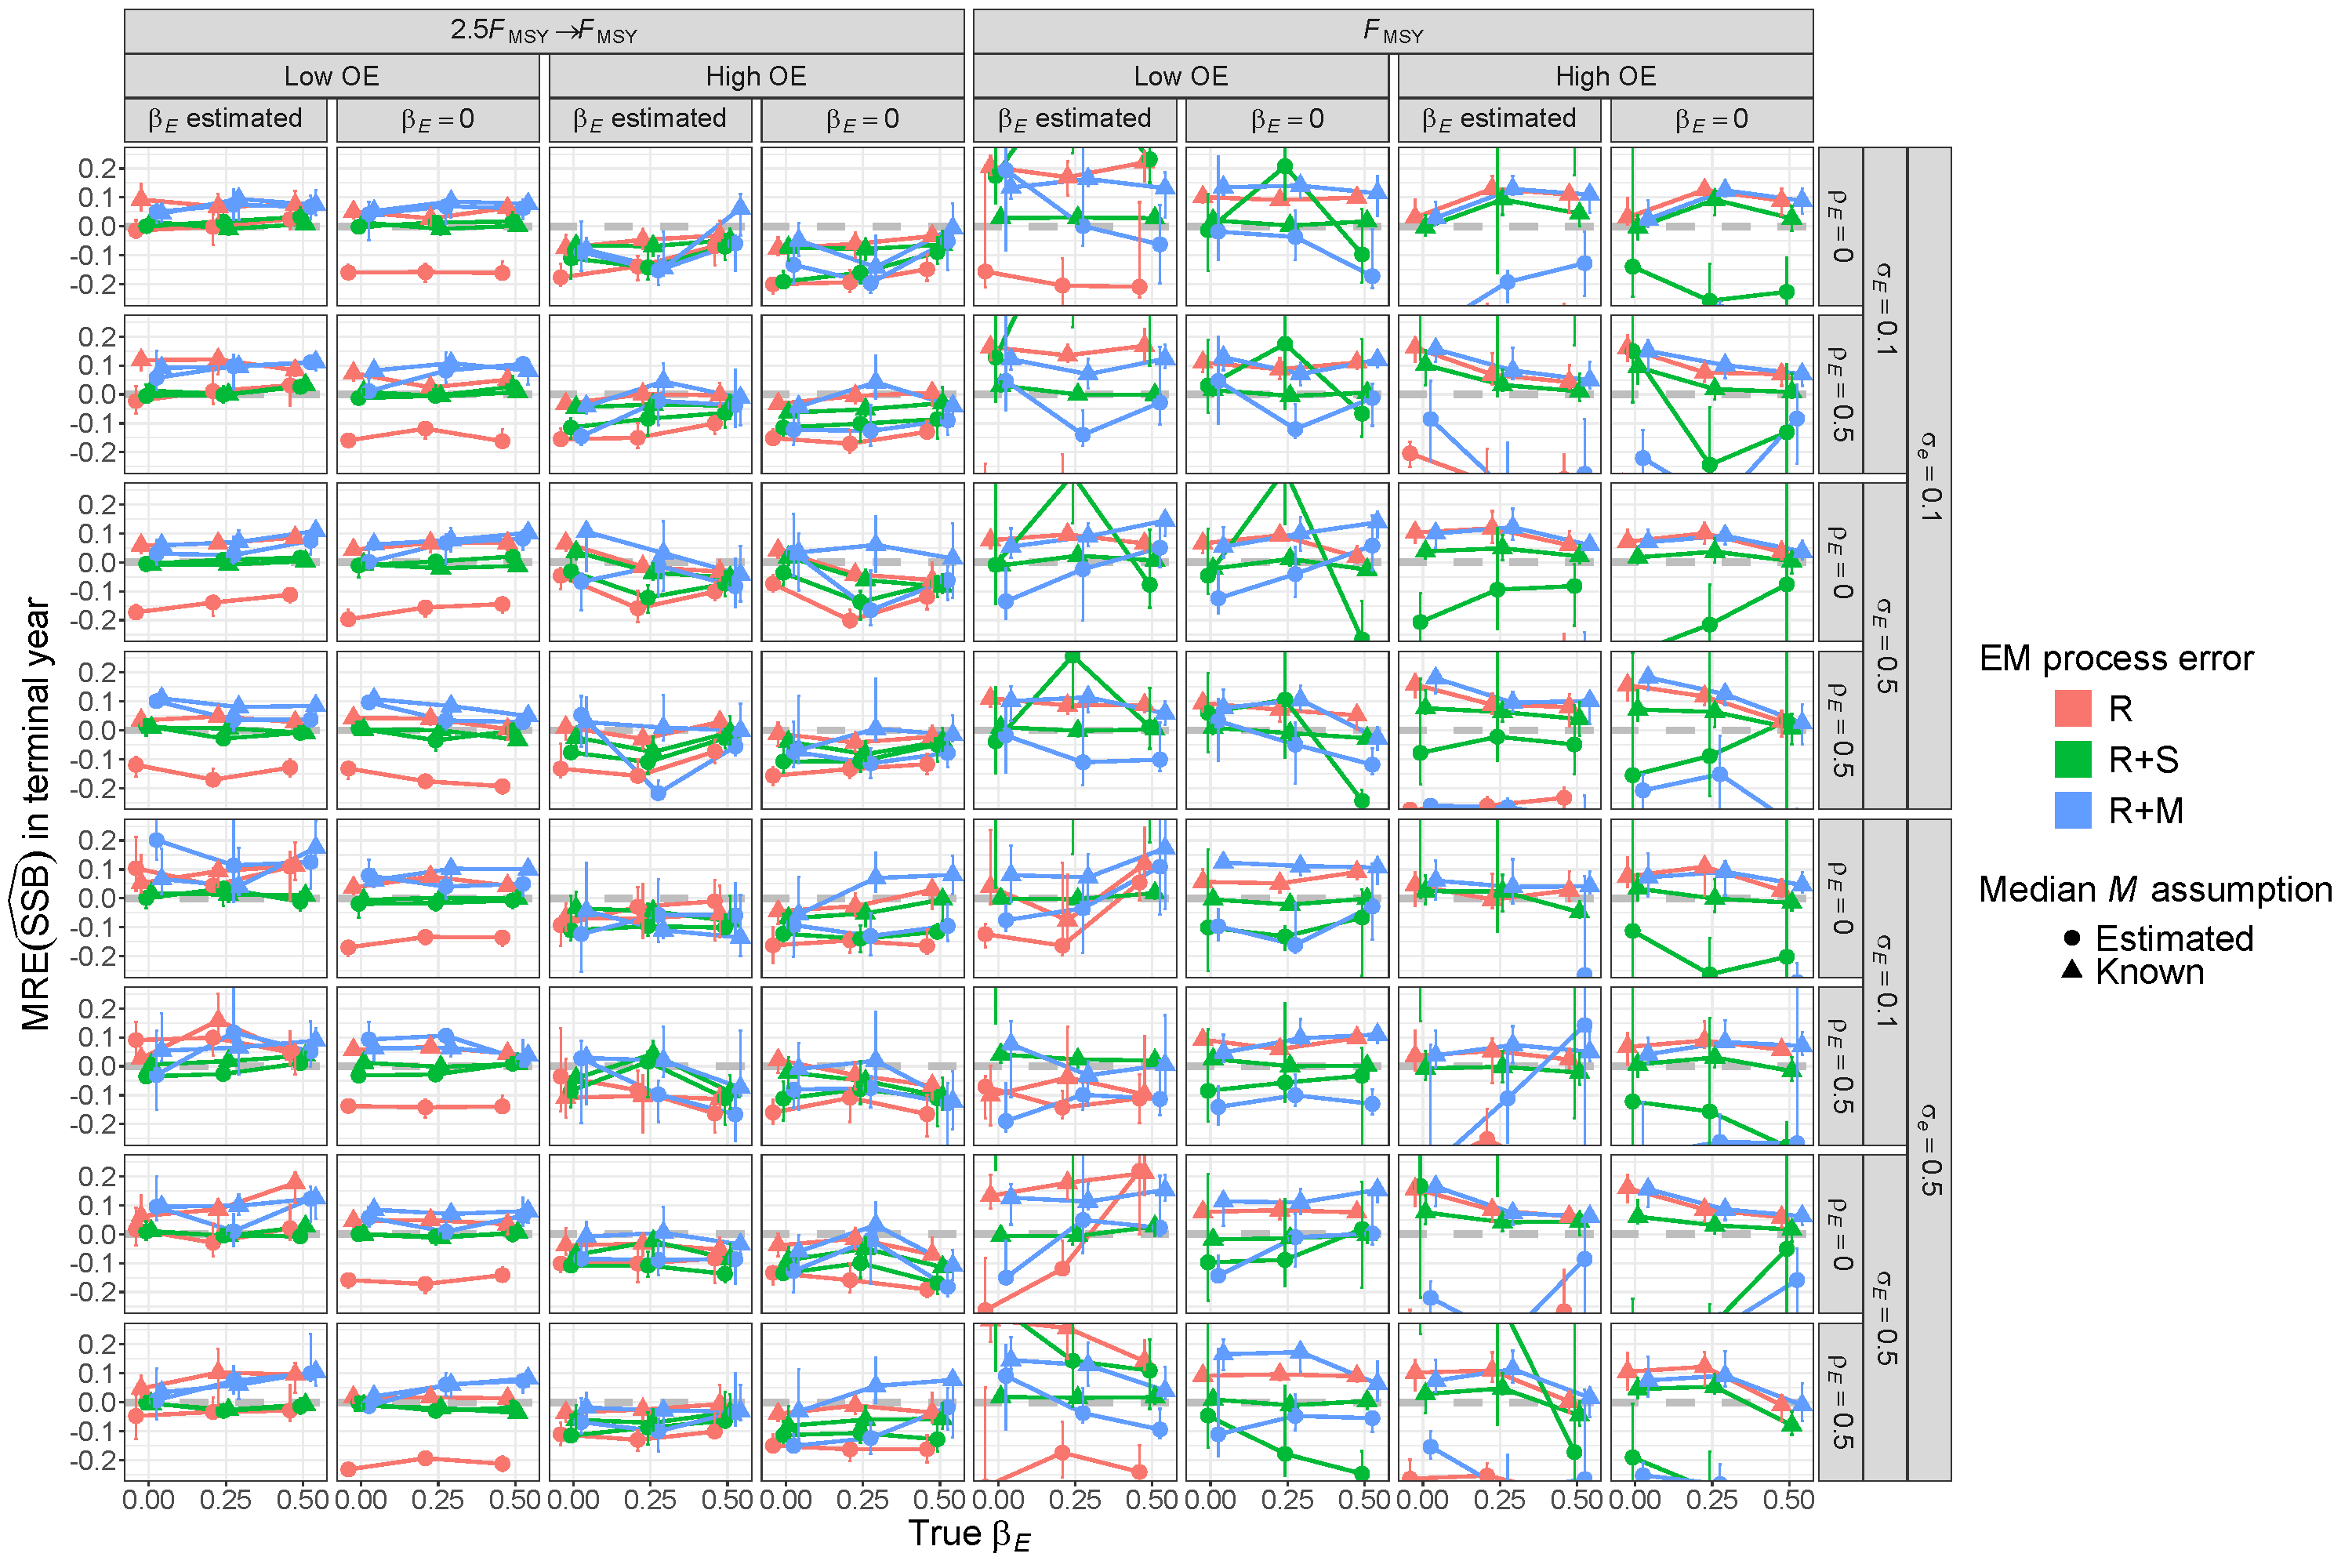
\includegraphics[height = \textheight]{terminal_year_ssb_bias_RSom}
\end{center}
\caption{\DIFaddFL{For R+S operating models, median relative error (MRE) of SSB in the terminal year for estimating models with alternative process error assumptions, treatment of covariate effect ($\beta_E = 0$ or estimated), and treatment of median $M$ parameter ($\beta_M$ estimated or known).}}\label{terminal_ssb_bias_RSom}
\end{figure}
\end{landscape}

\begin{landscape}
\begin{figure}
\begin{center}
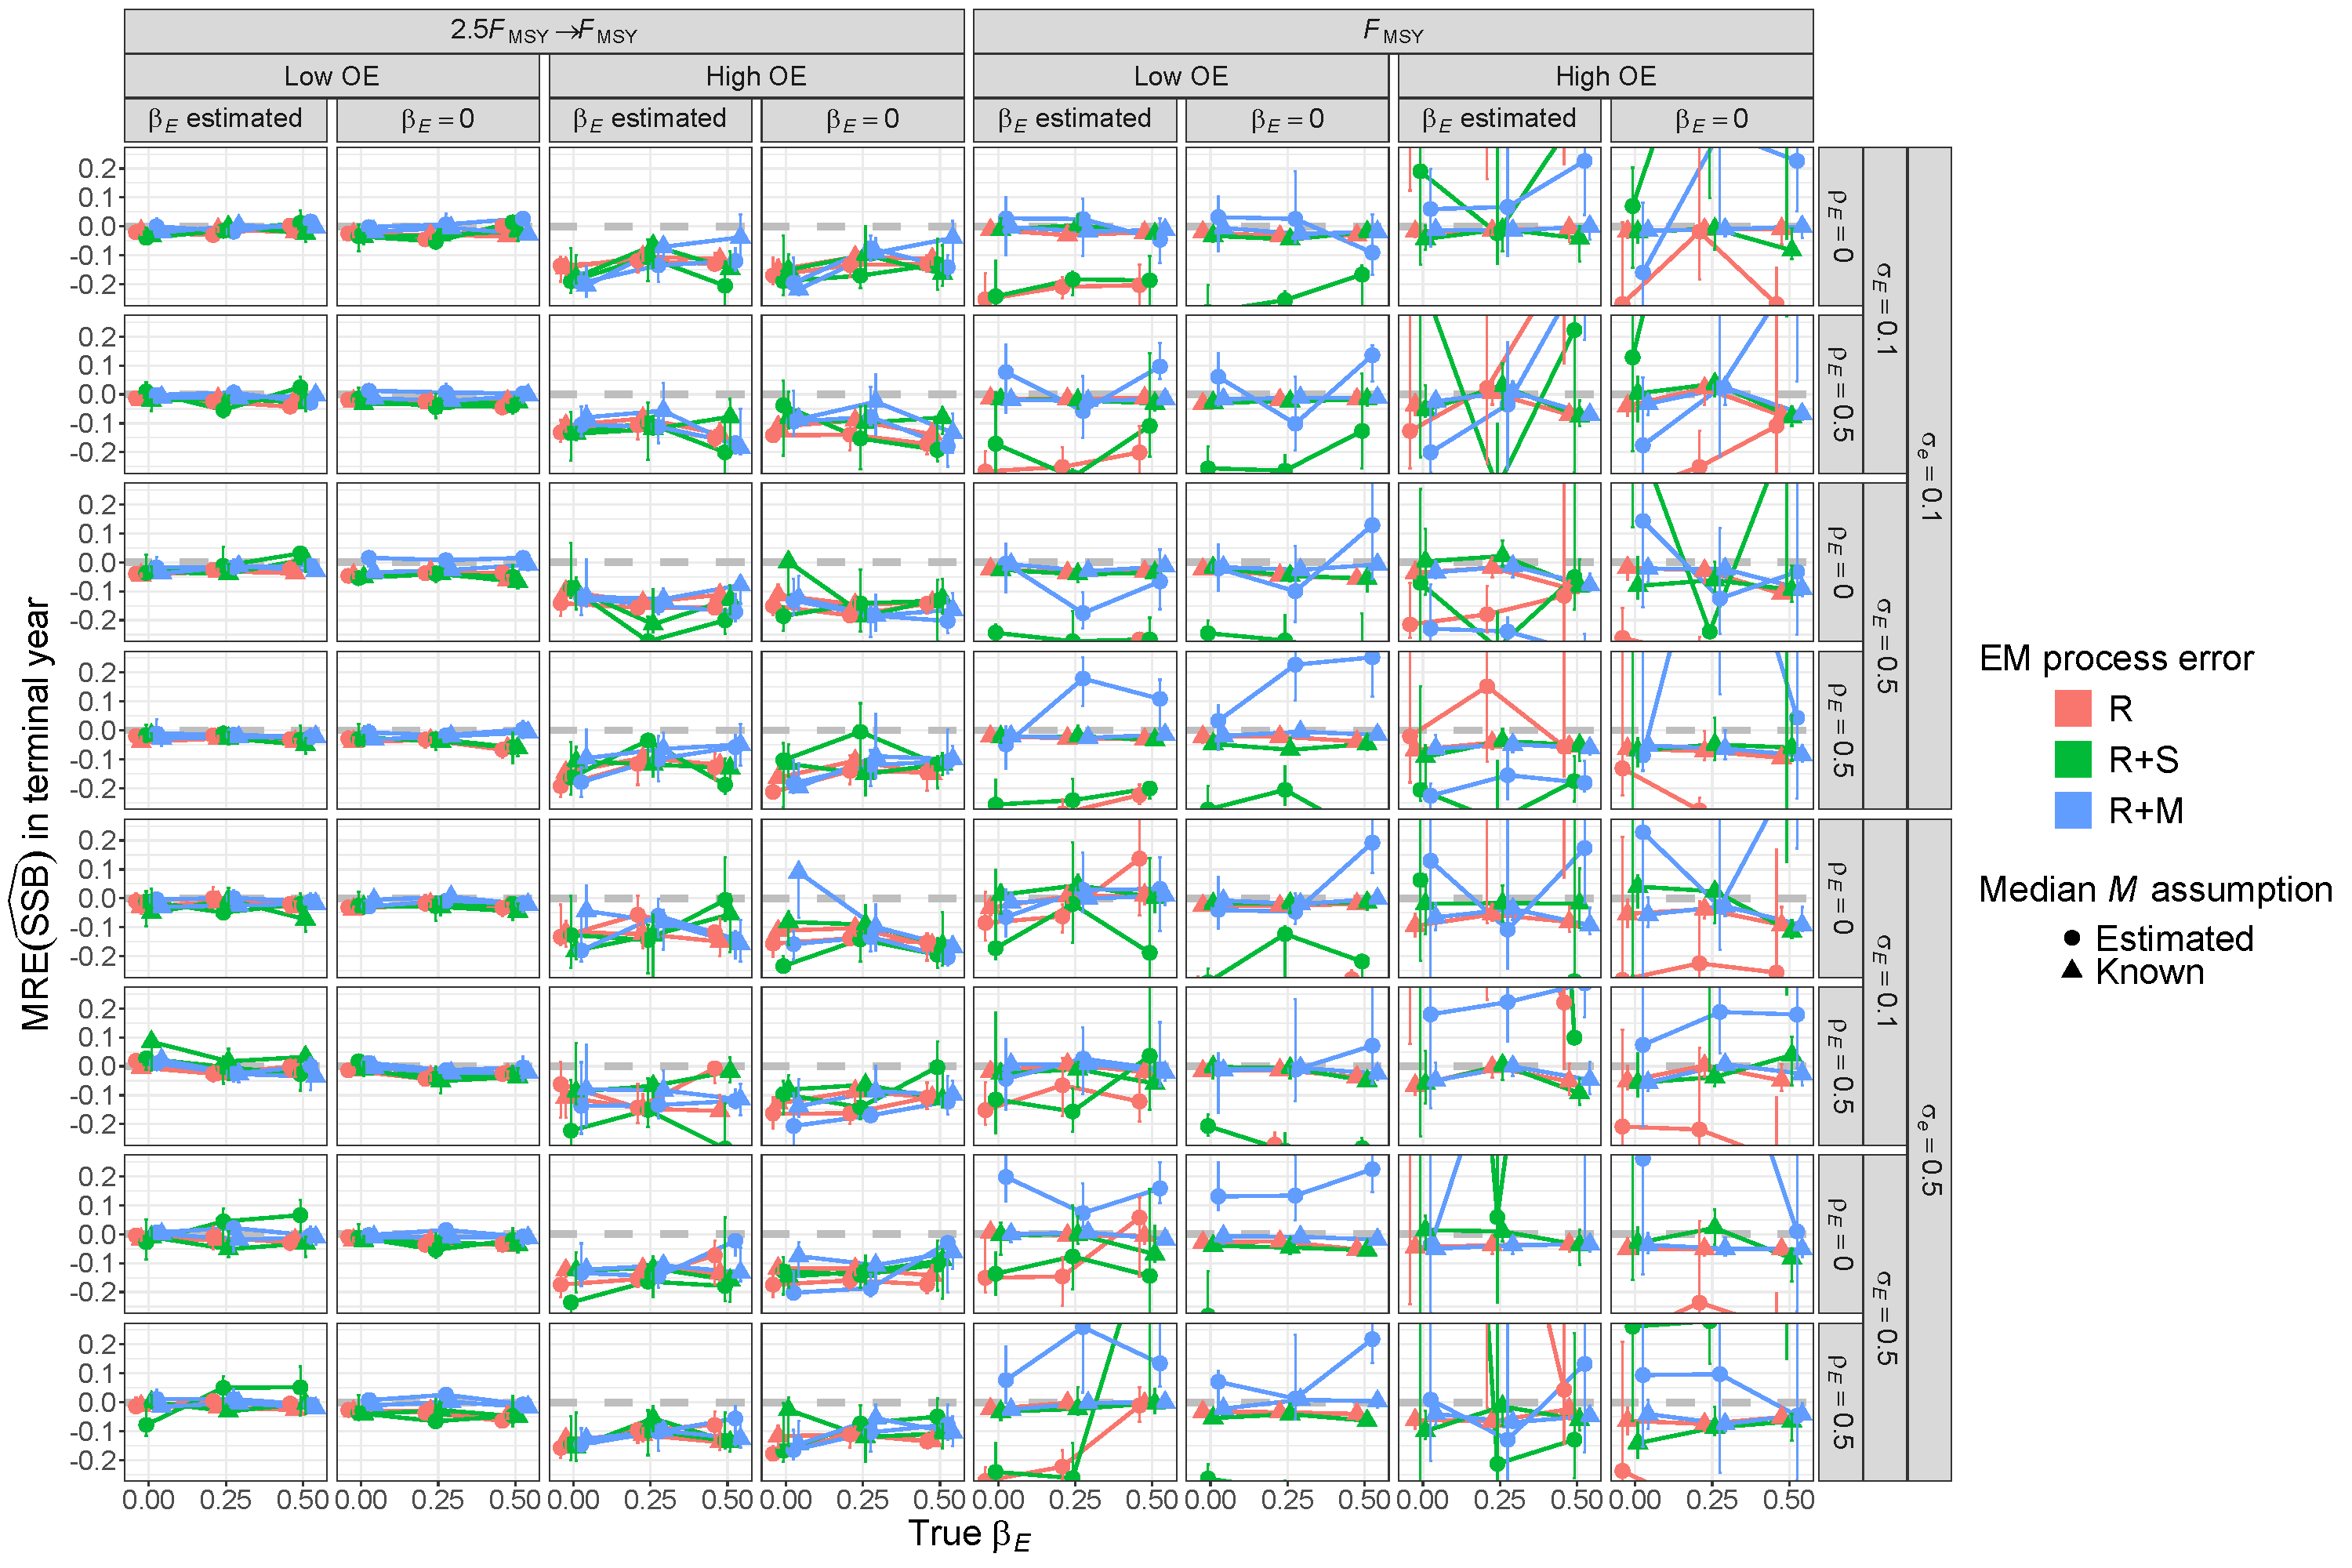
\includegraphics[height = \textheight]{terminal_year_ssb_bias_RMom}
\end{center}
\caption{\DIFaddFL{For R+M operating models, median relative error (MRE) of estimates of SSB in the terminal year for estimating models with alternative process error assumptions, treatment of covariate effect ($\beta_E = 0$ or estimated), and treatment of median $M$ parameter ($\beta_M$ estimated or known).}}\label{terminal_ssb_bias_RMom}
\end{figure}
\end{landscape}

\DIFaddend \begin{table}
\caption{\DIFdelbeginFL \DIFdelFL{Percent reduction in deviance for logistic regression models fit to indicators of convergence }\DIFdelendFL \DIFaddbeginFL \DIFaddFL{Operating }\DIFaddendFL (\DIFdelbeginFL \DIFdelFL{providing Hessian-based standard errors). Table rows give each operating model (}\DIFdelendFL OM) and estimating model (EM) \DIFdelbeginFL \DIFdelFL{factor included individually, combined, }\DIFdelendFL \DIFaddbeginFL \DIFaddFL{attributes used in analyses of deviance reduction }\DIFaddendFL and \DIFdelbeginFL \DIFdelFL{with second }\DIFdelendFL \DIFaddbeginFL \DIFaddFL{classification }\DIFaddendFL and \DIFdelbeginFL \DIFdelFL{third order interactions}\DIFdelendFL \DIFaddbeginFL \DIFaddFL{regression trees}\DIFaddendFL . \DIFdelbeginFL \DIFdelFL{Table columns are operating }\DIFdelendFL \DIFaddbeginFL \DIFaddFL{R, R+S, and R+M, denote }\DIFaddendFL models (\DIFdelbeginFL \DIFdelFL{OMs}\DIFdelendFL \DIFaddbeginFL \DIFaddFL{OM or EM}\DIFaddendFL ) with process error on recruitment only\DIFdelbeginFL \DIFdelFL{(R)}\DIFdelendFL , recruitment and apparent survival\DIFdelbeginFL \DIFdelFL{(R+S)}\DIFdelendFL , \DIFdelbeginFL \DIFdelFL{or }\DIFdelendFL \DIFaddbeginFL \DIFaddFL{and }\DIFaddendFL recruitment and natural mortality\DIFdelbeginFL \DIFdelFL{(R}\DIFdelendFL \DIFaddbeginFL \DIFaddFL{, respectively. SD denotes standard deviation and }\Fmsy \DIFaddFL{is the fishing mortality rate that acheives maximum sustainable yield.}}\label{factor_table}
{\begin{center}
\begin{tabular}{lc}
\hline\hline
\multicolumn{1}{c}{\DIFaddFL{Factor}}&\multicolumn{1}{c}{\DIFaddFL{Levels}}\tabularnewline
\hline
\DIFaddFL{OM Process error}&\DIFaddFL{R, R}\DIFaddendFL +\DIFaddbeginFL \DIFaddFL{S, R+}\DIFaddendFL M\DIFaddbeginFL \tabularnewline
\DIFaddFL{OM Fishing History}&\DIFaddFL{$F_{\text{MSY}}$, $2.5F_{\text{MSY}} \rightarrow F_{\text{MSY}}$}\tabularnewline
\DIFaddFL{OM Covariate effect size ($\beta_E$}\DIFaddendFL )\DIFdelbeginFL \DIFdelFL{.}%DIFDELCMD < \MBLOCKRIGHTBRACE%%%
\DIFdelendFL \DIFaddbeginFL &\DIFaddFL{0, 0.25, 0.5}\tabularnewline
\DIFaddFL{OM Population Observation Error}&\DIFaddFL{Low, High}\tabularnewline
\DIFaddFL{OM Covariate Observation Error}&\DIFaddFL{Low ($\sigma_e = 0.1$), High ($\sigma_e = 0.5$)}\tabularnewline
\DIFaddFL{OM Covariate Process Error SD ($\sigma_E$)}&\DIFaddFL{0.1, 0.5}\tabularnewline
\DIFaddFL{OM Covariate Process Error Correlation ($\rho_E$)}&\DIFaddFL{0, 0.5}\tabularnewline
\DIFaddFL{EM Process Error}&\DIFaddFL{R, R+S, R+M}\tabularnewline
\DIFaddFL{EM Covariate Effect}&\DIFaddFL{None ($\beta_E = 0$), $\beta_E$ estimated}\tabularnewline
\DIFaddFL{EM Median Natural Mortality Rate Parameter ($\beta_M$)}&\DIFaddFL{Known, Estimated}\tabularnewline
\hline
\end{tabular}\end{center}
}
\end{table}
\pagebreak

\begin{landscape}
\end{landscape}

\subsection*{\DIFadd{Percent deviance reduction results}}\label{percent-deviance-reduction-results}
\addcontentsline{toc}{subsection}{\DIFadd{Percent deviance reduction results}}

\subsubsection*{\DIFadd{Estimating model convergence}}\label{estimating-model-convergence}
\addcontentsline{toc}{subsubsection}{\DIFadd{Estimating model convergence}}

\DIFadd{For fitted logistic regression models to indicators of convergence, the estimating model process error assumption provided the largest percent reduction in deviance (9-25\%) of all operating model and estimating model attributes for all three operating model process error types (Table \ref{convergence_PRD_table}). Including second order interactions of operating model and estimating model factors also provided further reduction of residual deviance (between 7 and 11\%), indicating successful convergence depended on a combination of operating model and estimating model attributes.
}

\subsubsection*{\DIFadd{AIC performance of process error source selection}}\label{aic-performance-of-process-error-source-selection}
\addcontentsline{toc}{subsubsection}{\DIFadd{AIC performance of process error source selection}}

\DIFadd{For all OM process error types, the level of error in both the population and covariate observations were the attributes that resulted in the largest percent reductions in deviance for multinomial regression fits to indicators of AIC selection of the process error configuration (Table \ref{AIC_PE_PRD_table}). For R+S and R+M OMs, level of error in population observations provided deviance reduction (19\% and 13\%, respectively) much larger than any other OM and EM factors whereas error in covariate observations provided the largest reduction (8\%) for R OMs. Lesser deviance reduction (2-3\%) occurred for the true covariate effect size and whether the EM made the correct assumption about including a covariate effect for R OMs and error in covariate observations for R+M OMs. Including second and third order interactions, provided the largest reductions in residual deviance for R OMs (24\%) and little reduction for R+S and R+M OMs (4\% and 6\%, respectively).
}

\subsubsection*{\DIFadd{AIC performance of covariate effect selection}}\label{aic-performance-of-covariate-effect-selection}
\addcontentsline{toc}{subsubsection}{\DIFadd{AIC performance of covariate effect selection}}

\DIFadd{The factors explaining the largest reduction in deviance for logistic regression models fitted to indicators of AIC selection of the correct covariate effect assumption depended on the magnitude of the true effect assumed in the OM (Table \ref{AIC_Ecov_effect_PRD_table}). When OMs had no covariate effect (\(\beta_E = 0\)) the OM process errror type provided the largest reduction in deviance (4\%). When OMs assumed a covariate effect (\(\beta_E>0\)), level of error in population observations and magnitude of temporal variability in the true covariate provided the largest reductions in deviance (4\% and 8-21\%, respectively). The reduction in deviance provided by the magnitude of covariate temporal variability also increased with larger true covariate effect. Including second and third order interactions provided a modest reduction in deviance (5-7\%).
}

\subsubsection*{\DIFadd{Median natural mortality rate bias}}\label{median-natural-mortality-rate-bias}
\addcontentsline{toc}{subsubsection}{\DIFadd{Median natural mortality rate bias}}

\DIFadd{Across all OM process error types, regression models fit to errors in \(\widehat \beta_M\) showed largest reductions in deviance from the type of OM fishing pressure (4-17\%), EM process error assumption (2-12\%), and the EM covariate effect assumption (3-7\%, Table \ref{bias_median_M_converged_PRD_table}). The level of observation error also provided a similar reduction in deviance for R OMs (3\%). Relatively large reductions in deviance also occurred with second and third order interactions (7-16\%).
}

\subsubsection*{\DIFadd{Median natural mortality rate standard error bias}}\label{median-natural-mortality-rate-standard-error-bias}
\addcontentsline{toc}{subsubsection}{\DIFadd{Median natural mortality rate standard error bias}}

\DIFadd{The EM process error assumption provided the largest reduction in deviance for regression models fitted to errors in \(\widehat {\text{SE}}\left(\widehat \beta_M\right)\) from R (3\%) and R+M (7\%) OM simulations (Table \ref{median_M_se_bias_PRD_table}). The type of OM fishing pressure provided the largest reduction (13\%) for R+S OMs and a lesser reduction in devaince for R+M OMs (4\%). The EM covariate effect assumption also provided similar reductions in deviance for R+S (9\%) and R+M (4\%) OMs.
}

\subsubsection*{\DIFadd{Median natural mortality rate confidence interval bias}}\label{median-natural-mortality-rate-confidence-interval-bias}
\addcontentsline{toc}{subsubsection}{\DIFadd{Median natural mortality rate confidence interval bias}}

\DIFadd{For logistic regressions of indicators of CIs including \(\beta_M\), factors that provided the largest reductions in deviance were the OM fishing history and level of error in population observations for all OM process error types (0.3-6\%) (Table \ref{mean_M_ci_coverage_PRD_table}). Including second and third order interactions provided the largest relative increase in deviance reduction for R+S (8-11\%) and R+M OMs (5-8\%) and lesser increases for R OMs (3-5\%).
}

\subsubsection*{\DIFadd{Covariate effect bias}}\label{covariate-effect-bias}
\addcontentsline{toc}{subsubsection}{\DIFadd{Covariate effect bias}}

\DIFadd{For regression models fit to errors in estimation of \(\beta_E\), we found very little reduction in deviance for any of the OM and EM factors (Table \ref{bias_ecov_beta_converged_PRD_table}). For the normal model in these regressions, deviance is the sum of squares and there were extremely large estimates of \(\beta_E\) (and errors) for many simulations which resulted in extremely large sums of squares and relative differences from the null model were therefore small (\textless1\%). Nevertheless, observation error of the covariate provided either the largest or second largest reductions in deviance of any of the single OM and EM attributes for OM process error configuration types. OM fishing history provided reductions of similar scale for R and R+S OMs. Other factors providing similar reductions were true covariate effect size for R OMs and level of error in population observations and EM process error assumption for R+S OMs. Including second and third order interactions also provided further reductions in residual deviance similar in scale to the individual factors.
}

\subsubsection*{\DIFadd{Covariate effect standard error bias}}\label{covariate-effect-standard-error-bias}
\addcontentsline{toc}{subsubsection}{\DIFadd{Covariate effect standard error bias}}

\DIFadd{Factors providing the largest reductions in deviance for estimation error of \(\widehat {\text{SE}}\left(\widehat\beta_E\right)\) were generally similar to those that were most important for estimation of \(\beta_E\), but deviance reductions were one or two orders of magnitude larger (Table \ref{bias_ecov_beta_se_PRD_table}). Level of error in covariate observations and EM process error assumption was important for all OM process error configurations (6-13\% and 3-4\%, respectively). Level of error in population observations provided relatively large reductions in deviance for R+S and R+M OMs (3\% and 8\%, respectively). The OM fishing pressure history provided a lesser reduction in deviance for all OM process error types (2-4\%). Like estimation of \(\beta_E\), additional large reductions in deviance also occurred when second and third order interactions of OM and EM attributes were included in the regression models (11-31\%).
}

\subsubsection*{\DIFadd{Covariate effect confidence interval bias}}\label{covariate-effect-confidence-interval-bias}
\addcontentsline{toc}{subsubsection}{\DIFadd{Covariate effect confidence interval bias}}

\DIFadd{For logistic regressions of indicators of CIs including the true value of \(\beta_E\), factors that provided the largest reductions in deviance were true covariate effect size for R and R+M OMs (11\% and 3\%, respectively) and EM process error configuration for R+S OMs (7\%) (Table \ref{ecov_beta_ci_coverage_PRD_table}). Covariate observation error also provided relatively large reduction in deviance for R OMs (8\%). Lesser reductions of 1-2\% occurred for level of error in population observations and covariate temporal variability for all OM process error types. Including second and third order interactions also provided relatively large further reductions in deviance (5-9\%).
}

\subsubsection*{\DIFadd{Terminal year natural morality rate bias}}\label{terminal-year-natural-morality-rate-bias}
\addcontentsline{toc}{subsubsection}{\DIFadd{Terminal year natural morality rate bias}}

\DIFadd{Regressions of estimation errors show largest reductions in deviance from whether the EM treats \(\beta_M\) as known (Table \ref{bias_M_PRD_table}). For R and R+S OMs, annual \(M\) was constant, and therefore, terminal \(M\) was known when the true \(\beta_M\) was assumed known and there will be no error in any of those EMs. Beyond the \(\beta_M\) assumption, the OM fishing history, level of error in population observations, and EM assumptions for covariate effect and process error all provided notable deviance reductions.
}

\subsubsection*{\DIFadd{Terminal year natural morality rate accuracy}}\label{terminal-year-natural-morality-rate-accuracy}
\addcontentsline{toc}{subsubsection}{\DIFadd{Terminal year natural morality rate accuracy}}

\DIFadd{Like bias of terminal year \(M\), the EM assumption for \(\beta_M\) provided the largest reduction in deviance (22-45\%) for accuracy as measured by RMSE for all OM process error types (Table \ref{rmse_M_PRD_table}). Including second and third order interactions also provided large further reductions in deviance (21-38\%).
}

\DIFadd{Using correlation to measure accuracy of terminal year \(M\) estimation provides a different perspective. Treatment of \(\beta_M\) provided relatively large reductions in deviance for all OM process error types (3-12\%), but level of variability in the covariate was equally or more important (3-15\%) as was whether the covariate effect was included in the EM (12\%) for R and R+S OMs (Table \ref{corr_M_PRD_table}). Including second and third order interactions also provided relatively large ruther reductions in deviance (15 to 24\%).
}

\subsubsection*{\DIFadd{Terminal year spawning stock biomass bias}}\label{terminal-year-spawning-stock-biomass-bias}
\addcontentsline{toc}{subsubsection}{\DIFadd{Terminal year spawning stock biomass bias}}

\DIFadd{Regression model fits showed largest reductions in deviance for OM fishing history (2-3\%), error in population observations (1\% for R and R+M OMs), and EM \(\beta_M\) assumption (2\%; Table \ref{bias_SSB_PRD_table}). The type of EM process error assumed also provided a deviance reduction similar in scale for R+S OMs (1\%). Including second and third order interactions of OM and EM attributes provided further deviance reductions of 5-10\%.
}

\subsubsection*{\DIFadd{Terminal year spawning stock biomass accuracy}}\label{terminal-year-spawning-stock-biomass-accuracy}
\addcontentsline{toc}{subsubsection}{\DIFadd{Terminal year spawning stock biomass accuracy}}

\DIFadd{Largest reductions in deviance were provided by whether \(\beta_M\) was known or estimated (20-21\%) and whether there was temporal contrast in fishing pressure (20-33\%) across all OM process error types (Table \ref{rmse_SSB_PRD_table}). Lesser reductions were also provided by the EM process error assumption for R and R+M OMs. Inclusion of second and third order interactions of OM and EM attributes provided further reductions in deviance of 26-40\%.
}

\DIFadd{Using correlation to measure accuracy, temporal contrast in fishing pressure and EM treatment of \(\beta_M\) provided relatively important reductions in deviance like RMSE, but level of error in population observations was important rather than EM process error type (Table \ref{corr_ssb_PRD_table}). Including second and third order interactions also provided relatively large ruther reductions in deviance (6 to 20\%).
}

\begin{table}
\caption{\DIFaddFL{Percent reduction in deviance for logistic regression models fit to indicators of convergence (providing Hessian-based standard errors). Table rows give each operating model (OM) and estimating model (EM) factor included individually, combined, and with second and third order interactions. Table columns categorize operating models (OMs) with process error on recruitment only (R), recruitment and apparent survival (R+S), or recruitment and natural mortality (R+M). See Table \ref{factor_table} for further details.}}\DIFaddendFL \label{convergence_PRD_table}
{\begin{center}
\begin{tabular}{lrrr}
\hline\hline
\multicolumn{1}{l}{Factor}&\multicolumn{1}{c}{R}&\multicolumn{1}{c}{R+S}&\multicolumn{1}{c}{R+M}\tabularnewline
\hline
OM $F$ history& 0.86&\textless  0.01& 0.24\tabularnewline
OM Obs. Error& 0.56& 0.03& 0.26\tabularnewline
OM $\sigma_e$& 0.66& 2.99& 0.93\tabularnewline
OM $\sigma_E$& 0.53& 2.22& 0.62\tabularnewline
OM $\rho_{E}$&\textless  0.01& 0.02&\textless  0.01\tabularnewline
OM $\beta_{E}$& 0.02&\textless  0.01&\textless  0.01\tabularnewline
EM Process Error&24.53& 9.33&23.06\tabularnewline
EM $\beta_{E}$ assumption& 0.16& 2.96& 0.51\tabularnewline
EM $M$ Assumption& 0.18& 2.83& 0.40\tabularnewline
All factors&28.92&22.67&27.34\tabularnewline
+ All Two Way&36.15&33.54&34.03\tabularnewline
+ All Three Way&37.95&36.58&35.57\tabularnewline
\hline
\end{tabular}\end{center}
}
\end{table}
\pagebreak

\begin{table}
\caption{Percent reduction in deviance for multinomial logistic regression models fit to indicators of process error assumption in the estimating models \DIFdelbeginFL \DIFdelFL{(EMs) }\DIFdelendFL with lowest AIC. \DIFdelbeginFL \DIFdelFL{Table rows give each operating model (OM) }\DIFdelendFL \DIFaddbeginFL \DIFaddFL{See Tables \ref{convergence_PRD_table} }\DIFaddendFL and \DIFdelbeginFL \DIFdelFL{estimating model (EM) factor included individually, combined, and with second and third order interactions}\DIFdelendFL \DIFaddbeginFL \DIFaddFL{\ref{factor_table} for further details}\DIFaddendFL .\DIFdelbeginFL \DIFdelFL{Table columns are operating models (OMs) with process error on recruitment only (R), recruitment and apparent survival (R+S), or recruitment and natural mortality (R+M).}\DIFdelendFL }\label{AIC_PE_PRD_table}
{\begin{center}
\begin{tabular}{lrrr}
\hline\hline
\multicolumn{1}{l}{Factor}&\multicolumn{1}{c}{R}&\multicolumn{1}{c}{R+S}&\multicolumn{1}{c}{R+M}\tabularnewline
\hline
OM $F$ history& 0.23& 0.06& 0.30\tabularnewline
OM Obs. Error& 0.54&18.58&13.43\tabularnewline
OM $\sigma_e$& 8.41& 0.05& 2.23\tabularnewline
OM $\sigma_E$& 0.17& 0.08& 0.59\tabularnewline
OM $\rho_{E}$& 1.29& 0.03& 0.06\tabularnewline
OM $\beta_{E}$& 3.42& 0.04& 0.38\tabularnewline
EM $M$ Assumption& 0.35& 0.34& 0.48\tabularnewline
EM $\beta_{E}$ Assumption Correct& 2.35& 0.22& 0.78\tabularnewline
All factors&21.97&19.29&19.07\tabularnewline
+ All Two Way&38.25&21.13&24.73\tabularnewline
+ All Three Way&46.26&22.85&26.97\tabularnewline
\hline
\end{tabular}\end{center}
}
\end{table}
\pagebreak

\begin{table}
\caption{Percent reduction in deviance for logistic regression models fit to indicators of correct estimating model (EM) covariate effect assumption (no effect \DIFdelbeginFL \DIFdelFL{with OM }\DIFdelendFL \DIFaddbeginFL \DIFaddFL{for operating models assuming }\DIFaddendFL $\beta_E = 0$ or estimated effect \DIFdelbeginFL \DIFdelFL{when OM }\DIFdelendFL \DIFaddbeginFL \DIFaddFL{for operating models assuming }\DIFaddendFL $\beta_E > 0$) with lowest AIC. Table \DIFdelbeginFL \DIFdelFL{rows give each operating model (OM) and estimating model (EM) factor included individually, combined, and with second and third order interactions. Table }\DIFdelendFL columns \DIFdelbeginFL \DIFdelFL{are }\DIFdelendFL \DIFaddbeginFL \DIFaddFL{categorize }\DIFaddendFL operating models \DIFdelbeginFL \DIFdelFL{(OMs) }\DIFdelendFL with \DIFdelbeginFL \DIFdelFL{process error on recruitment only (R), recruitment }\DIFdelendFL \DIFaddbeginFL \DIFaddFL{different true values for $\beta_E$. See Tables \ref{convergence_PRD_table} }\DIFaddendFL and \DIFdelbeginFL \DIFdelFL{apparent survival (R+S), or recruitment and natural mortality (R+M)}\DIFdelendFL \DIFaddbeginFL \DIFaddFL{\ref{factor_table} for further details}\DIFaddendFL .}\label{AIC_Ecov_effect_PRD_table}
{\begin{center}
\begin{tabular}{lrrr}
\hline\hline
\multicolumn{1}{l}{Factor}&\multicolumn{1}{c}{$\beta_E = 0$}&\multicolumn{1}{c}{$\beta_E = 0.25$}&\multicolumn{1}{c}{$\beta_E = 0.5$}\tabularnewline
\hline
OM $F$ history&\textless  0.01& 0.09& 0.18\tabularnewline
OM Obs. Error& 1.19& 4.06& 4.64\tabularnewline
OM Process Error& 4.11& 0.71& 0.25\tabularnewline
OM $\sigma_e$& 0.66& 2.00& 1.97\tabularnewline
OM $\sigma_E$& 0.35& 7.97&20.66\tabularnewline
OM $\rho_{E}$& 0.21& 1.23& 1.48\tabularnewline
EM $M$ Assumption& 0.23& 0.15& 0.15\tabularnewline
EM Process Error Assumption Correct& 1.95& 0.39& 0.06\tabularnewline
All factors& 6.95&17.65&33.44\tabularnewline
+ All Two Way&10.58&23.21&38.36\tabularnewline
+ All Three Way&11.83&24.95&39.79\tabularnewline
\hline
\end{tabular}\end{center}
}
\end{table}
\pagebreak

\begin{table}
\caption{Percent reduction in deviance for linear regression models fit to errors in estimation of the \DIFdelbeginFL \DIFdelFL{covariate effect on }\DIFdelendFL \DIFaddbeginFL \DIFaddFL{median }\DIFaddendFL natural mortality rate \DIFaddbeginFL \DIFaddFL{parameter }\DIFaddendFL (\DIFdelbeginFL \DIFdelFL{$\widehat \beta_E$}\DIFdelendFL \DIFaddbeginFL \DIFaddFL{$\widehat \beta_M$}\DIFaddendFL ). \DIFdelbeginFL \DIFdelFL{Table rows give each operating model (OM) }\DIFdelendFL \DIFaddbeginFL \DIFaddFL{See Tables \ref{convergence_PRD_table} }\DIFaddendFL and \DIFdelbeginFL \DIFdelFL{estimating model (EM) factor included individually, combined, and with second and third order interactions}\DIFdelendFL \DIFaddbeginFL \DIFaddFL{\ref{factor_table} for further details}\DIFaddendFL .\DIFdelbeginFL \DIFdelFL{Table columns are operating models (OMs) with process error on recruitment only (R), recruitment and apparent survival (R+S), or recruitment and natural mortality (R+M).}\DIFdelendFL }\DIFdelbeginFL %DIFDELCMD < \label{bias_ecov_beta_converged_PRD_table}
%DIFDELCMD < %%%
\DIFdelendFL \DIFaddbeginFL \label{bias_median_M_converged_PRD_table}
\DIFaddendFL {\begin{center}
\begin{tabular}{lrrr}
\hline\hline
\multicolumn{1}{l}{Factor}&\multicolumn{1}{c}{R}&\multicolumn{1}{c}{R+S}&\multicolumn{1}{c}{R+M}\tabularnewline
\hline
OM $F$ history& \DIFdelbeginFL \DIFdelFL{0.03}\DIFdelendFL \DIFaddbeginFL \DIFaddFL{4.03}\DIFaddendFL &\DIFdelbeginFL \DIFdelFL{0.06}\DIFdelendFL \DIFaddbeginFL \DIFaddFL{16.52}\DIFaddendFL & \DIFdelbeginFL \DIFdelFL{0.02}\DIFdelendFL \DIFaddbeginFL \DIFaddFL{6.51}\DIFaddendFL \tabularnewline
OM Obs. Error& \DIFdelbeginFL \DIFdelFL{\textless  0.01}\DIFdelendFL \DIFaddbeginFL \DIFaddFL{2.74}\DIFaddendFL & \DIFdelbeginFL \DIFdelFL{0.06}\DIFdelendFL \DIFaddbeginFL \DIFaddFL{0.54}\DIFaddendFL & \DIFdelbeginFL \DIFdelFL{0.02}\DIFdelendFL \DIFaddbeginFL \DIFaddFL{0.64}\DIFaddendFL \tabularnewline
OM $\sigma_e$& \DIFdelbeginFL \DIFdelFL{0.04}\DIFdelendFL \DIFaddbeginFL \DIFaddFL{0.01}\DIFaddendFL &\DIFdelbeginFL \DIFdelFL{0.08}\DIFdelendFL \DIFaddbeginFL \DIFaddFL{\textless  0.01}\DIFaddendFL & \DIFdelbeginFL \DIFdelFL{0.06}\DIFdelendFL \DIFaddbeginFL \DIFaddFL{0.01}\DIFaddendFL \tabularnewline
OM $\sigma_E$& \DIFdelbeginFL \DIFdelFL{\textless  0.01}\DIFdelendFL \DIFaddbeginFL \DIFaddFL{0.18}\DIFaddendFL & 0.02& \DIFdelbeginFL \DIFdelFL{0.01}\DIFdelendFL \DIFaddbeginFL \DIFaddFL{0.15}\DIFaddendFL \tabularnewline
OM $\rho_{E}$& \DIFdelbeginFL \DIFdelFL{\textless  0.01}\DIFdelendFL \DIFaddbeginFL \DIFaddFL{0.07}\DIFaddendFL & \DIFdelbeginFL \DIFdelFL{0.01}\DIFdelendFL \DIFaddbeginFL \DIFaddFL{0.05}\DIFaddendFL &\textless  0.01\tabularnewline
OM $\beta_{E}$& \DIFdelbeginFL \DIFdelFL{0.05}\DIFdelendFL \DIFaddbeginFL \DIFaddFL{0.37}\DIFaddendFL & \DIFdelbeginFL \DIFdelFL{\textless  0.01}\DIFdelendFL \DIFaddbeginFL \DIFaddFL{0.04}\DIFaddendFL & \DIFdelbeginFL \DIFdelFL{\textless  0.01}\DIFdelendFL \DIFaddbeginFL \DIFaddFL{0.10}\DIFaddendFL \tabularnewline
EM Process Error& \DIFdelbeginFL \DIFdelFL{0.01}\DIFdelendFL \DIFaddbeginFL \DIFaddFL{2.31}\DIFaddendFL &\DIFdelbeginFL \DIFdelFL{0.06}\DIFdelendFL \DIFaddbeginFL \DIFaddFL{11.99}\DIFaddendFL & \DIFdelbeginFL \DIFdelFL{0.01}\DIFdelendFL \DIFaddbeginFL \DIFaddFL{2.65}\DIFaddendFL \tabularnewline
EM \DIFdelbeginFL \DIFdelFL{$M$ }\DIFdelendFL \DIFaddbeginFL \DIFaddFL{$\beta_{E}$ }\DIFaddendFL assumption& \DIFdelbeginFL \DIFdelFL{0.02}\DIFdelendFL \DIFaddbeginFL \DIFaddFL{2.83}\DIFaddendFL & \DIFdelbeginFL \DIFdelFL{0.02}\DIFdelendFL \DIFaddbeginFL \DIFaddFL{7.20}\DIFaddendFL & \DIFdelbeginFL \DIFdelFL{\textless  0.01}\DIFdelendFL \DIFaddbeginFL \DIFaddFL{3.25}\DIFaddendFL \tabularnewline
All factors&\DIFdelbeginFL \DIFdelFL{0.18}\DIFdelendFL \DIFaddbeginFL \DIFaddFL{12.14}\DIFaddendFL &\DIFdelbeginFL \DIFdelFL{0.37}\DIFdelendFL \DIFaddbeginFL \DIFaddFL{33.71}\DIFaddendFL &\DIFdelbeginFL \DIFdelFL{0.14}\DIFdelendFL \DIFaddbeginFL \DIFaddFL{12.81}\DIFaddendFL \tabularnewline
+ All Two Way&\DIFdelbeginFL \DIFdelFL{0.50}\DIFdelendFL \DIFaddbeginFL \DIFaddFL{21.74}\DIFaddendFL &\DIFdelbeginFL \DIFdelFL{1.11}\DIFdelendFL \DIFaddbeginFL \DIFaddFL{46.46}\DIFaddendFL &\DIFdelbeginFL \DIFdelFL{0.35}\DIFdelendFL \DIFaddbeginFL \DIFaddFL{19.84}\DIFaddendFL \tabularnewline
+ All Three Way&\DIFdelbeginFL \DIFdelFL{1.38}\DIFdelendFL \DIFaddbeginFL \DIFaddFL{26.38}\DIFaddendFL &\DIFdelbeginFL \DIFdelFL{1.88}\DIFdelendFL \DIFaddbeginFL \DIFaddFL{49.41}\DIFaddendFL &\DIFdelbeginFL \DIFdelFL{0.66}\DIFdelendFL \DIFaddbeginFL \DIFaddFL{22.24}\DIFaddendFL \tabularnewline
\hline
\end{tabular}\end{center}
}
\end{table}
\pagebreak

\begin{table}
\caption{Percent reduction in deviance for \DIFdelbeginFL \DIFdelFL{logistic }\DIFdelendFL \DIFaddbeginFL \DIFaddFL{linear }\DIFaddendFL regression models fit to \DIFdelbeginFL \DIFdelFL{indicators }\DIFdelendFL \DIFaddbeginFL \DIFaddFL{errors in estimation }\DIFaddendFL of \DIFdelbeginFL \DIFdelFL{whether confidence intervals for covariate effect estimates includes }\DIFdelendFL the \DIFdelbeginFL \DIFdelFL{true value. Table rows give each operating model (OM) and estimating model (EM) factor included individually, combined, and with second and third order interactions. Table columns are operating models (OMs) with process }\DIFdelendFL \DIFaddbeginFL \DIFaddFL{Hessian-based standard }\DIFaddendFL error \DIFdelbeginFL \DIFdelFL{on recruitment only }\DIFdelendFL \DIFaddbeginFL \DIFaddFL{of the median $M$ parameter }\DIFaddendFL (\DIFdelbeginFL \DIFdelFL{R}\DIFdelendFL \DIFaddbeginFL \DIFaddFL{$\widehat {\text{SE}}\left(\widehat \beta_M\right)$}\DIFaddendFL )\DIFdelbeginFL \DIFdelFL{, recruitment }\DIFdelendFL \DIFaddbeginFL \DIFaddFL{. See Tables \ref{convergence_PRD_table} }\DIFaddendFL and \DIFdelbeginFL \DIFdelFL{apparent survival (R+S), or recruitment and natural mortality (R+M)}\DIFdelendFL \DIFaddbeginFL \DIFaddFL{\ref{factor_table} for further details}\DIFaddendFL .}\DIFdelbeginFL %DIFDELCMD < \label{ecov_beta_ci_coverage_PRD_table}
%DIFDELCMD < %%%
\DIFdelendFL \DIFaddbeginFL \label{median_M_se_bias_PRD_table}
\DIFaddendFL {\begin{center}
\begin{tabular}{lrrr}
\hline\hline
\multicolumn{1}{l}{Factor}&\multicolumn{1}{c}{R}&\multicolumn{1}{c}{R+S}&\multicolumn{1}{c}{R+M}\tabularnewline
\hline
OM $F$ history& \DIFdelbeginFL \DIFdelFL{0.24}\DIFdelendFL \DIFaddbeginFL \DIFaddFL{0.55}\DIFaddendFL &\DIFdelbeginFL \DIFdelFL{0.05}\DIFdelendFL \DIFaddbeginFL \DIFaddFL{12.91}\DIFaddendFL & \DIFdelbeginFL \DIFdelFL{0.01}\DIFdelendFL \DIFaddbeginFL \DIFaddFL{3.65}\DIFaddendFL \tabularnewline
OM Obs. Error& \DIFdelbeginFL \DIFdelFL{1.36}\DIFdelendFL \DIFaddbeginFL \DIFaddFL{0.98}\DIFaddendFL & \DIFdelbeginFL \DIFdelFL{1.91}\DIFdelendFL \DIFaddbeginFL \DIFaddFL{0.01}\DIFaddendFL & \DIFdelbeginFL \DIFdelFL{1.78}\DIFdelendFL \DIFaddbeginFL \DIFaddFL{0.07}\DIFaddendFL \tabularnewline
OM $\sigma_e$&\DIFdelbeginFL \DIFdelFL{8.26}\DIFdelendFL \DIFaddbeginFL \DIFaddFL{\textless  0.01}\DIFaddendFL & \DIFdelbeginFL \DIFdelFL{0.24}\DIFdelendFL \DIFaddbeginFL \DIFaddFL{0.03}\DIFaddendFL & \DIFdelbeginFL \DIFdelFL{0.92}\DIFdelendFL \DIFaddbeginFL \DIFaddFL{0.11}\DIFaddendFL \tabularnewline
OM $\sigma_E$& \DIFdelbeginFL \DIFdelFL{0.92}\DIFdelendFL \DIFaddbeginFL \DIFaddFL{0.13}\DIFaddendFL & \DIFdelbeginFL \DIFdelFL{1.70}\DIFdelendFL \DIFaddbeginFL \DIFaddFL{0.03}\DIFaddendFL & \DIFdelbeginFL \DIFdelFL{1.56}\DIFdelendFL \DIFaddbeginFL \DIFaddFL{0.19}\DIFaddendFL \tabularnewline
OM $\rho_{E}$&\DIFdelbeginFL \DIFdelFL{0.03}%DIFDELCMD < & %%%
\DIFdelFL{0.05}%DIFDELCMD < & %%%
\DIFdelFL{0.06}%DIFDELCMD < \tabularnewline
%DIFDELCMD < %%%
\DIFdelFL{OM $\beta_{E}$}%DIFDELCMD < &%%%
\DIFdelFL{11.10}%DIFDELCMD < & %%%
\DIFdelFL{0.68}%DIFDELCMD < & %%%
\DIFdelFL{2.72}%DIFDELCMD < \tabularnewline
%DIFDELCMD < %%%
\DIFdelFL{EM Process Error}%DIFDELCMD < & %%%
\DIFdelFL{0.01}%DIFDELCMD < & %%%
\DIFdelFL{6.51}%DIFDELCMD < & %%%
\DIFdelFL{0.27}%DIFDELCMD < \tabularnewline
%DIFDELCMD < %%%
\DIFdelFL{EM $M$ assumption}%DIFDELCMD < & %%%
\DIFdelFL{0.25}%DIFDELCMD < & %%%
\DIFdelFL{0.29}%DIFDELCMD < & %%%
\DIFdelFL{0.06}%DIFDELCMD < \tabularnewline
%DIFDELCMD < %%%
\DIFdelFL{All factors}%DIFDELCMD < &%%%
\DIFdelFL{23.61}%DIFDELCMD < &%%%
\DIFdelFL{12.16}%DIFDELCMD < & %%%
\DIFdelFL{7.78}%DIFDELCMD < \tabularnewline
%DIFDELCMD < %%%
\DIFdelFL{+ All Two Way}%DIFDELCMD < &%%%
\DIFdelFL{30.17}%DIFDELCMD < &%%%
\DIFdelFL{18.08}%DIFDELCMD < &%%%
\DIFdelFL{12.63}%DIFDELCMD < \tabularnewline
%DIFDELCMD < %%%
\DIFdelFL{+ All Three Way}%DIFDELCMD < &%%%
\DIFdelFL{32.58}%DIFDELCMD < &%%%
\DIFdelFL{20.62}%DIFDELCMD < &%%%
\DIFdelFL{14.87}%DIFDELCMD < \tabularnewline
%DIFDELCMD < \hline
%DIFDELCMD < \end{tabular}\end{center}
%DIFDELCMD < }
%DIFDELCMD < \end{table}
%DIFDELCMD < \pagebreak
%DIFDELCMD < 

%DIFDELCMD < \begin{table}
%DIFDELCMD < %%%
%DIFDELCMD < \caption{%
{%DIFAUXCMD
\DIFdelFL{Percent reduction in deviance for linear regression models fit to errors in estimation of the median natural mortality rate parameter ($\widehat \beta_M$). Table rows give each operating model (OM) and estimating model (EM) factor included individually, combined, and with second and third order interactions. Table columns are operating models (OMs) with process error on recruitment only (R), recruitment and apparent survival (R+S), or recruitment and natural mortality (R+M).}}%DIFAUXCMD
%DIFDELCMD < \label{bias_median_M_converged_PRD_table}
%DIFDELCMD < {\begin{center}
%DIFDELCMD < \begin{tabular}{lrrr}
%DIFDELCMD < \hline\hline
%DIFDELCMD < %%%
%DIFDELCMD < \multicolumn{1}{l}{%
{%DIFAUXCMD
\DIFdelFL{Factor}}%DIFAUXCMD
%DIFDELCMD < &%%%
%DIFDELCMD < \multicolumn{1}{c}{%
{%DIFAUXCMD
\DIFdelFL{R}}%DIFAUXCMD
%DIFDELCMD < &%%%
%DIFDELCMD < \multicolumn{1}{c}{%
{%DIFAUXCMD
\DIFdelFL{R+S}}%DIFAUXCMD
%DIFDELCMD < &%%%
%DIFDELCMD < \multicolumn{1}{c}{%
{%DIFAUXCMD
\DIFdelFL{R+M}}%DIFAUXCMD
%DIFDELCMD < \tabularnewline
%DIFDELCMD < \hline
%DIFDELCMD < %%%
\DIFdelFL{OM $F$ history}%DIFDELCMD < & %%%
\DIFdelFL{4.03}%DIFDELCMD < &%%%
\DIFdelFL{16.52}%DIFDELCMD < & %%%
\DIFdelFL{6.51}%DIFDELCMD < \tabularnewline
%DIFDELCMD < %%%
\DIFdelFL{OM Obs. Error}%DIFDELCMD < & %%%
\DIFdelFL{2.74}%DIFDELCMD < & %%%
\DIFdelFL{0.54}%DIFDELCMD < & %%%
\DIFdelFL{0.64}%DIFDELCMD < \tabularnewline
%DIFDELCMD < %%%
\DIFdelFL{OM $\sigma_e$}%DIFDELCMD < & %%%
\DIFdelFL{0.01}%DIFDELCMD < &%%%
\DIFdelendFL \textless  0.01& \DIFdelbeginFL \DIFdelFL{0.01}%DIFDELCMD < \tabularnewline
%DIFDELCMD < %%%
\DIFdelFL{OM $\sigma_E$}%DIFDELCMD < & %%%
\DIFdelFL{0.18}%DIFDELCMD < & %%%
\DIFdelendFL 0.02&\DIFdelbeginFL \DIFdelFL{0.15}%DIFDELCMD < \tabularnewline
%DIFDELCMD < %%%
\DIFdelFL{OM $\rho_{E}$}%DIFDELCMD < & %%%
\DIFdelFL{0.07}%DIFDELCMD < & %%%
\DIFdelFL{0.05}%DIFDELCMD < &%%%
\DIFdelendFL \textless  0.01\tabularnewline
OM $\beta_{E}$& \DIFdelbeginFL \DIFdelFL{0.37}\DIFdelendFL \DIFaddbeginFL \DIFaddFL{0.12}\DIFaddendFL & \DIFdelbeginFL \DIFdelFL{0.04}\DIFdelendFL \DIFaddbeginFL \DIFaddFL{0.07}\DIFaddendFL & \DIFdelbeginFL \DIFdelFL{0.10}\DIFdelendFL \DIFaddbeginFL \DIFaddFL{0.23}\DIFaddendFL \tabularnewline
EM Process Error& \DIFdelbeginFL \DIFdelFL{2.31}\DIFdelendFL \DIFaddbeginFL \DIFaddFL{3.16}\DIFaddendFL & \DIFdelbeginFL \DIFdelFL{11.99}\DIFdelendFL \DIFaddbeginFL \DIFaddFL{8.79}\DIFaddendFL & \DIFdelbeginFL \DIFdelFL{2.65}\DIFdelendFL \DIFaddbeginFL \DIFaddFL{6.83}\DIFaddendFL \tabularnewline
EM $\beta_{E}$ assumption& \DIFdelbeginFL \DIFdelFL{2.83}\DIFdelendFL \DIFaddbeginFL \DIFaddFL{0.18}\DIFaddendFL & \DIFdelbeginFL \DIFdelFL{7.20}\DIFdelendFL \DIFaddbeginFL \DIFaddFL{8.96}\DIFaddendFL & \DIFdelbeginFL \DIFdelFL{3.25}\DIFdelendFL \DIFaddbeginFL \DIFaddFL{3.81}\DIFaddendFL \tabularnewline
All factors& \DIFdelbeginFL \DIFdelFL{12.14}\DIFdelendFL \DIFaddbeginFL \DIFaddFL{5.32}\DIFaddendFL &\DIFdelbeginFL \DIFdelFL{33.71}\DIFdelendFL \DIFaddbeginFL \DIFaddFL{28.39}\DIFaddendFL &\DIFdelbeginFL \DIFdelFL{12.81}\DIFdelendFL \DIFaddbeginFL \DIFaddFL{14.71}\DIFaddendFL \tabularnewline
+ All Two Way&\DIFdelbeginFL \DIFdelFL{21.74}\DIFdelendFL \DIFaddbeginFL \DIFaddFL{11.80}\DIFaddendFL &\DIFdelbeginFL \DIFdelFL{46.46}\DIFdelendFL \DIFaddbeginFL \DIFaddFL{44.67}\DIFaddendFL &\DIFdelbeginFL \DIFdelFL{19.84}\DIFdelendFL \DIFaddbeginFL \DIFaddFL{22.70}\DIFaddendFL \tabularnewline
+ All Three Way&\DIFdelbeginFL \DIFdelFL{26.38}\DIFdelendFL \DIFaddbeginFL \DIFaddFL{17.83}\DIFaddendFL &\DIFdelbeginFL \DIFdelFL{49.41}\DIFdelendFL \DIFaddbeginFL \DIFaddFL{51.54}\DIFaddendFL &\DIFdelbeginFL \DIFdelFL{22.24}\DIFdelendFL \DIFaddbeginFL \DIFaddFL{29.46}\DIFaddendFL \tabularnewline
\hline
\end{tabular}\end{center}
}
\end{table}
\pagebreak

\begin{table}
\caption{Percent reduction in deviance for logistic regression models fit to indicators of whether \DIFdelbeginFL \DIFdelFL{confidence intervals }\DIFdelendFL \DIFaddbeginFL \DIFaddFL{CIs }\DIFaddendFL for estimates of the median natural mortality rate parameter ($\widehat \beta_M$) includes the true value. \DIFdelbeginFL \DIFdelFL{Table rows give each operating model (OM) }\DIFdelendFL \DIFaddbeginFL \DIFaddFL{See Tables \ref{convergence_PRD_table} }\DIFaddendFL and \DIFdelbeginFL \DIFdelFL{estimating model (EM) factor included individually, combined, and with second and third order interactions}\DIFdelendFL \DIFaddbeginFL \DIFaddFL{\ref{factor_table} for further details}\DIFaddendFL .\DIFdelbeginFL \DIFdelFL{Table columns are operating models (OMs) with process error on recruitment only (R), recruitment and apparent survival (R+S), or recruitment and natural mortality (R+M).}\DIFdelendFL }\label{mean_M_ci_coverage_PRD_table}
{\begin{center}
\begin{tabular}{lrrr}
\hline\hline
\multicolumn{1}{l}{Factor}&\multicolumn{1}{c}{R}&\multicolumn{1}{c}{R+S}&\multicolumn{1}{c}{R+M}\tabularnewline
\hline
OM $F$ history& 6.08& 1.46& 0.14\tabularnewline
OM Obs. Error& 1.48& 0.41& 0.29\tabularnewline
OM $\sigma_e$& 0.01& 0.06& 0.01\tabularnewline
OM $\sigma_E$& 0.13& 0.02& 0.04\tabularnewline
OM $\rho_{E}$&\textless  0.01&\textless  0.01& 0.02\tabularnewline
OM $\beta_{E}$& 0.08& 0.11& 0.09\tabularnewline
EM Process Error& 0.53& 0.08& 0.04\tabularnewline
EM $\beta_{E}$ assumption&\textless  0.01& 0.19& 0.01\tabularnewline
All factors& 8.46& 2.32& 0.62\tabularnewline
+ All Two Way&11.97&10.57& 5.99\tabularnewline
+ All Three Way&13.35&13.51& 8.44\tabularnewline
\hline
\end{tabular}\end{center}
}
\end{table}
\pagebreak

\begin{table}
\caption{Percent reduction in deviance for linear regression models fit to errors in estimation \DIFdelbeginFL \DIFdelFL{measured by Eq. \ref{relerror_trans_response} for }\DIFdelendFL \DIFaddbeginFL \DIFaddFL{of }\DIFaddendFL the \DIFdelbeginFL \DIFdelFL{terminal year }\DIFdelendFL \DIFaddbeginFL \DIFaddFL{covariate effect on }\DIFaddendFL natural mortality rate (\DIFdelbeginFL \DIFdelFL{$M$}\DIFdelendFL \DIFaddbeginFL \DIFaddFL{$\widehat \beta_E$}\DIFaddendFL ). \DIFdelbeginFL \DIFdelFL{Table rows give each operating model (OM) }\DIFdelendFL \DIFaddbeginFL \DIFaddFL{See Tables \ref{convergence_PRD_table} }\DIFaddendFL and \DIFdelbeginFL \DIFdelFL{estimating model (EM) factor included individually, combined, and with second and third order interactions}\DIFdelendFL \DIFaddbeginFL \DIFaddFL{\ref{factor_table} for further details}\DIFaddendFL .\DIFdelbeginFL \DIFdelFL{Table columns are operating models (OMs) with process error on recruitment only (R), recruitment and apparent survival (R+S), or recruitment and natural mortality (R+M).}\DIFdelendFL }\DIFdelbeginFL %DIFDELCMD < \label{bias_M_PRD_table}
%DIFDELCMD < %%%
\DIFdelendFL \DIFaddbeginFL \label{bias_ecov_beta_converged_PRD_table}
\DIFaddendFL {\begin{center}
\begin{tabular}{lrrr}
\hline\hline
\multicolumn{1}{l}{Factor}&\multicolumn{1}{c}{R}&\multicolumn{1}{c}{R+S}&\multicolumn{1}{c}{R+M}\tabularnewline
\hline
\DIFdelbeginFL \DIFdelFL{Convergence}%DIFDELCMD < &%%%
\DIFdelFL{\textless  0.01}%DIFDELCMD < & %%%
\DIFdelFL{0.18}%DIFDELCMD < & %%%
\DIFdelFL{0.01}%DIFDELCMD < \tabularnewline
%DIFDELCMD < %%%
\DIFdelendFL OM $F$ history&\DIFdelbeginFL \DIFdelFL{0.66}\DIFdelendFL \DIFaddbeginFL \DIFaddFL{0.03}\DIFaddendFL &\DIFdelbeginFL \DIFdelFL{2.69}\DIFdelendFL \DIFaddbeginFL \DIFaddFL{0.06}\DIFaddendFL &\DIFdelbeginFL \DIFdelFL{1.00}\DIFdelendFL \DIFaddbeginFL \DIFaddFL{0.02}\DIFaddendFL \tabularnewline
OM Obs. Error&\DIFdelbeginFL \DIFdelFL{0.29}\DIFdelendFL \DIFaddbeginFL \DIFaddFL{\textless  0.01}\DIFaddendFL &\DIFdelbeginFL \DIFdelFL{0.43}\DIFdelendFL \DIFaddbeginFL \DIFaddFL{0.06}\DIFaddendFL &\DIFdelbeginFL \DIFdelFL{0.16}\DIFdelendFL \DIFaddbeginFL \DIFaddFL{0.02}\DIFaddendFL \tabularnewline
OM $\sigma_e$&\DIFdelbeginFL \DIFdelFL{\textless  0.01}\DIFdelendFL \DIFaddbeginFL \DIFaddFL{0.04}\DIFaddendFL &\DIFdelbeginFL \DIFdelFL{\textless  0.01}\DIFdelendFL \DIFaddbeginFL \DIFaddFL{0.08}\DIFaddendFL &\DIFdelbeginFL \DIFdelFL{\textless  0.01}\DIFdelendFL \DIFaddbeginFL \DIFaddFL{0.06}\DIFaddendFL \tabularnewline
OM $\sigma_E$&\DIFdelbeginFL \DIFdelFL{0.02}%DIFDELCMD < &%%%
\DIFdelendFL \textless  0.01&\DIFdelbeginFL \DIFdelFL{\textless  }\DIFdelendFL \DIFaddbeginFL \DIFaddFL{0.02}&\DIFaddendFL 0.01\tabularnewline
OM $\rho_{E}$&\textless  0.01&0.01&\textless  0.01\tabularnewline
OM $\beta_{E}$&\DIFdelbeginFL \DIFdelFL{0.03}\DIFdelendFL \DIFaddbeginFL \DIFaddFL{0.05}\DIFaddendFL &\DIFaddbeginFL \DIFaddFL{\textless  }\DIFaddendFL 0.01&\DIFaddbeginFL \DIFaddFL{\textless  }\DIFaddendFL 0.01\tabularnewline
EM Process Error&\DIFdelbeginFL \DIFdelFL{0.22}\DIFdelendFL \DIFaddbeginFL \DIFaddFL{0.01}\DIFaddendFL &\DIFdelbeginFL \DIFdelFL{1.42}\DIFdelendFL \DIFaddbeginFL \DIFaddFL{0.06}\DIFaddendFL &\DIFdelbeginFL \DIFdelFL{0.43}\DIFdelendFL \DIFaddbeginFL \DIFaddFL{0.01}\DIFaddendFL \tabularnewline
EM \DIFdelbeginFL \DIFdelFL{$\beta_{E}$ assumption}%DIFDELCMD < & %%%
\DIFdelFL{0.35}%DIFDELCMD < & %%%
\DIFdelFL{1.07}%DIFDELCMD < & %%%
\DIFdelFL{0.39}%DIFDELCMD < \tabularnewline
%DIFDELCMD < %%%
\DIFdelFL{EM }\DIFdelendFL $M$ assumption&\DIFdelbeginFL \DIFdelFL{0.84}\DIFdelendFL \DIFaddbeginFL \DIFaddFL{0.02}\DIFaddendFL &\DIFdelbeginFL \DIFdelFL{5.10}\DIFdelendFL \DIFaddbeginFL \DIFaddFL{0.02}\DIFaddendFL &\DIFdelbeginFL \DIFdelFL{1.22}\DIFdelendFL \DIFaddbeginFL \DIFaddFL{\textless  0.01}\DIFaddendFL \tabularnewline
All factors&\DIFdelbeginFL \DIFdelFL{2.56}\DIFdelendFL \DIFaddbeginFL \DIFaddFL{0.18}\DIFaddendFL &\DIFdelbeginFL \DIFdelFL{10.83}\DIFdelendFL \DIFaddbeginFL \DIFaddFL{0.37}\DIFaddendFL &\DIFdelbeginFL \DIFdelFL{3.37}\DIFdelendFL \DIFaddbeginFL \DIFaddFL{0.14}\DIFaddendFL \tabularnewline
+ All Two Way&\DIFdelbeginFL \DIFdelFL{5.41}\DIFdelendFL \DIFaddbeginFL \DIFaddFL{0.50}\DIFaddendFL &\DIFdelbeginFL \DIFdelFL{18.75}\DIFdelendFL \DIFaddbeginFL \DIFaddFL{1.11}\DIFaddendFL &\DIFdelbeginFL \DIFdelFL{6.38}\DIFdelendFL \DIFaddbeginFL \DIFaddFL{0.35}\DIFaddendFL \tabularnewline
+ All Three Way&\DIFdelbeginFL \DIFdelFL{7.93}\DIFdelendFL \DIFaddbeginFL \DIFaddFL{1.38}\DIFaddendFL &\DIFdelbeginFL \DIFdelFL{22.49}\DIFdelendFL \DIFaddbeginFL \DIFaddFL{1.88}\DIFaddendFL &\DIFdelbeginFL \DIFdelFL{8.76}\DIFdelendFL \DIFaddbeginFL \DIFaddFL{0.66}\DIFaddendFL \tabularnewline
\hline
\end{tabular}\end{center}
}
\end{table}
\pagebreak

\begin{table}
\caption{Percent reduction in deviance for linear regression models fit to errors in estimation \DIFdelbeginFL \DIFdelFL{measured by Eq. \ref{relerror_trans_response} for }\DIFdelendFL \DIFaddbeginFL \DIFaddFL{of }\DIFaddendFL the \DIFdelbeginFL \DIFdelFL{terminal year spawning stock biomass (SSB). Table rows give each operating model (OM) and estimating model (EM) factor included individually, combined, and with second and third order interactions. Table columns are operating models (OMs) with process }\DIFdelendFL \DIFaddbeginFL \DIFaddFL{Hessian-based standard }\DIFaddendFL error \DIFaddbeginFL \DIFaddFL{of the covariate effect }\DIFaddendFL on \DIFdelbeginFL \DIFdelFL{recruitment only }\DIFdelendFL \DIFaddbeginFL \DIFaddFL{$M$ }\DIFaddendFL (\DIFdelbeginFL \DIFdelFL{R}\DIFdelendFL \DIFaddbeginFL \DIFaddFL{$\widehat {\text{SE}}\left(\widehat \beta_E\right)$}\DIFaddendFL )\DIFdelbeginFL \DIFdelFL{, recruitment }\DIFdelendFL \DIFaddbeginFL \DIFaddFL{. See Tables \ref{convergence_PRD_table} }\DIFaddendFL and \DIFdelbeginFL \DIFdelFL{apparent survival (R+S), or recruitment and natural mortality (R+M)}\DIFdelendFL \DIFaddbeginFL \DIFaddFL{\ref{factor_table} for further details}\DIFaddendFL .}\DIFdelbeginFL %DIFDELCMD < \label{bias_SSB_PRD_table}
%DIFDELCMD < %%%
\DIFdelendFL \DIFaddbeginFL \label{bias_ecov_beta_se_PRD_table}
\DIFaddendFL {\begin{center}
\begin{tabular}{lrrr}
\hline\hline
\multicolumn{1}{l}{Factor}&\multicolumn{1}{c}{R}&\multicolumn{1}{c}{R+S}&\multicolumn{1}{c}{R+M}\tabularnewline
\hline
\DIFdelbeginFL \DIFdelFL{Convergence}%DIFDELCMD < & %%%
\DIFdelFL{0.02}%DIFDELCMD < & %%%
\DIFdelFL{0.13}%DIFDELCMD < &%%%
\DIFdelFL{\textless  0.01}%DIFDELCMD < \tabularnewline
%DIFDELCMD < %%%
\DIFdelendFL OM $F$ history& \DIFdelbeginFL \DIFdelFL{2.08}\DIFdelendFL \DIFaddbeginFL \DIFaddFL{1.84}\DIFaddendFL & \DIFdelbeginFL \DIFdelFL{2.74}\DIFdelendFL \DIFaddbeginFL \DIFaddFL{2.68}\DIFaddendFL & \DIFdelbeginFL \DIFdelFL{1.75}\DIFdelendFL \DIFaddbeginFL \DIFaddFL{4.00}\DIFaddendFL \tabularnewline
OM Obs. Error& \DIFdelbeginFL \DIFdelFL{1.09}\DIFdelendFL \DIFaddbeginFL \DIFaddFL{0.06}\DIFaddendFL & \DIFdelbeginFL \DIFdelFL{0.18}\DIFdelendFL \DIFaddbeginFL \DIFaddFL{2.74}\DIFaddendFL & \DIFdelbeginFL \DIFdelFL{1.19}\DIFdelendFL \DIFaddbeginFL \DIFaddFL{8.04}\DIFaddendFL \tabularnewline
OM $\sigma_e$& \DIFdelbeginFL \DIFdelFL{0.01}\DIFdelendFL \DIFaddbeginFL \DIFaddFL{6.27}\DIFaddendFL & \DIFdelbeginFL \DIFdelFL{\textless  0.01}\DIFdelendFL \DIFaddbeginFL \DIFaddFL{7.28}\DIFaddendFL &\DIFdelbeginFL \DIFdelFL{\textless  0.01}\DIFdelendFL \DIFaddbeginFL \DIFaddFL{12.83}\DIFaddendFL \tabularnewline
OM $\sigma_E$& \DIFdelbeginFL \DIFdelFL{\textless  0.01}\DIFdelendFL \DIFaddbeginFL \DIFaddFL{0.48}\DIFaddendFL & \DIFdelbeginFL \DIFdelFL{\textless  0.01}\DIFdelendFL \DIFaddbeginFL \DIFaddFL{1.05}\DIFaddendFL & \DIFdelbeginFL \DIFdelFL{\textless  0.01}\DIFdelendFL \DIFaddbeginFL \DIFaddFL{0.46}\DIFaddendFL \tabularnewline
OM $\rho_{E}$& \DIFdelbeginFL \DIFdelFL{\textless  0.01}\DIFdelendFL \DIFaddbeginFL \DIFaddFL{0.17}\DIFaddendFL & \DIFdelbeginFL \DIFdelFL{\textless  }\DIFdelendFL 0.01& \DIFdelbeginFL \DIFdelFL{\textless  0.01}\DIFdelendFL \DIFaddbeginFL \DIFaddFL{0.02}\DIFaddendFL \tabularnewline
OM $\beta_{E}$& \DIFdelbeginFL \DIFdelFL{\textless  0.01}\DIFdelendFL \DIFaddbeginFL \DIFaddFL{0.37}\DIFaddendFL & 0.01& \DIFdelbeginFL \DIFdelFL{\textless  0.01}\DIFdelendFL \DIFaddbeginFL \DIFaddFL{0.05}\DIFaddendFL \tabularnewline
EM Process Error& \DIFdelbeginFL \DIFdelFL{0.52}\DIFdelendFL \DIFaddbeginFL \DIFaddFL{2.90}\DIFaddendFL & \DIFdelbeginFL \DIFdelFL{1.05}\DIFdelendFL \DIFaddbeginFL \DIFaddFL{3.89}\DIFaddendFL & \DIFdelbeginFL \DIFdelFL{0.57}\DIFdelendFL \DIFaddbeginFL \DIFaddFL{2.98}\DIFaddendFL \tabularnewline
EM \DIFdelbeginFL \DIFdelFL{$\beta_{E}$ assumption}%DIFDELCMD < &%%%
\DIFdelFL{\textless  0.01}%DIFDELCMD < & %%%
\DIFdelFL{0.05}%DIFDELCMD < & %%%
\DIFdelFL{0.01}%DIFDELCMD < \tabularnewline
%DIFDELCMD < %%%
\DIFdelFL{EM }\DIFdelendFL $M$ assumption& \DIFdelbeginFL \DIFdelFL{1.76}\DIFdelendFL \DIFaddbeginFL \DIFaddFL{0.15}\DIFaddendFL & \DIFdelbeginFL \DIFdelFL{2.12}\DIFdelendFL \DIFaddbeginFL \DIFaddFL{0.34}\DIFaddendFL & \DIFdelbeginFL \DIFdelFL{1.51}\DIFdelendFL \DIFaddbeginFL \DIFaddFL{0.47}\DIFaddendFL \tabularnewline
All factors&\DIFdelbeginFL \DIFdelFL{5.97}\DIFdelendFL \DIFaddbeginFL \DIFaddFL{13.01}\DIFaddendFL &\DIFdelbeginFL \DIFdelFL{6.58}\DIFdelendFL \DIFaddbeginFL \DIFaddFL{20.95}\DIFaddendFL &\DIFdelbeginFL \DIFdelFL{5.21}\DIFdelendFL \DIFaddbeginFL \DIFaddFL{29.24}\DIFaddendFL \tabularnewline
+ All Two Way&\DIFdelbeginFL \DIFdelFL{12.81}\DIFdelendFL \DIFaddbeginFL \DIFaddFL{28.58}\DIFaddendFL &\DIFdelbeginFL \DIFdelFL{13.00}\DIFdelendFL \DIFaddbeginFL \DIFaddFL{32.25}\DIFaddendFL &\DIFdelbeginFL \DIFdelFL{11.97}\DIFdelendFL \DIFaddbeginFL \DIFaddFL{42.77}\DIFaddendFL \tabularnewline
+ All Three Way&\DIFdelbeginFL \DIFdelFL{16.41}\DIFdelendFL \DIFaddbeginFL \DIFaddFL{44.44}\DIFaddendFL &\DIFdelbeginFL \DIFdelFL{15.57}\DIFdelendFL \DIFaddbeginFL \DIFaddFL{42.83}\DIFaddendFL &\DIFdelbeginFL \DIFdelFL{15.73}\DIFdelendFL \DIFaddbeginFL \DIFaddFL{51.84}\DIFaddendFL \tabularnewline
\hline
\end{tabular}\end{center}
}
\end{table}
\pagebreak

\DIFdelbegin %DIFDELCMD < \setcounter{figure}{0}
%DIFDELCMD < \renewcommand\thefigure{S\arabic{figure}}
%DIFDELCMD < 

%DIFDELCMD < \setcounter{table}{0}
%DIFDELCMD < \renewcommand\thetable{S\arabic{table}}
%DIFDELCMD < 

%DIFDELCMD < \begin{landscape}
%DIFDELCMD < \end{landscape}
%DIFDELCMD < 

%DIFDELCMD < %%%
\section*{\DIFdel{Supplemental Materials}}%DIFAUXCMD
%DIFDELCMD < \label{supplemental-materials}
%DIFDELCMD < %%%
\addcontentsline{toc}{section}{\DIFdel{Supplemental Materials}}
%DIFAUXCMD
%DIFDELCMD < 

%DIFDELCMD < %%%
\subsection*{\DIFdel{Referenced Figures and Tables}}%DIFAUXCMD
%DIFDELCMD < \label{referenced-figures-and-tables}
%DIFDELCMD < %%%
\addcontentsline{toc}{subsection}{\DIFdel{Referenced Figures and Tables}}
%DIFAUXCMD
%DIFDELCMD < 

%DIFDELCMD < \begin{landscape}
%DIFDELCMD < \begin{figure}
%DIFDELCMD < \begin{center}
%DIFDELCMD < 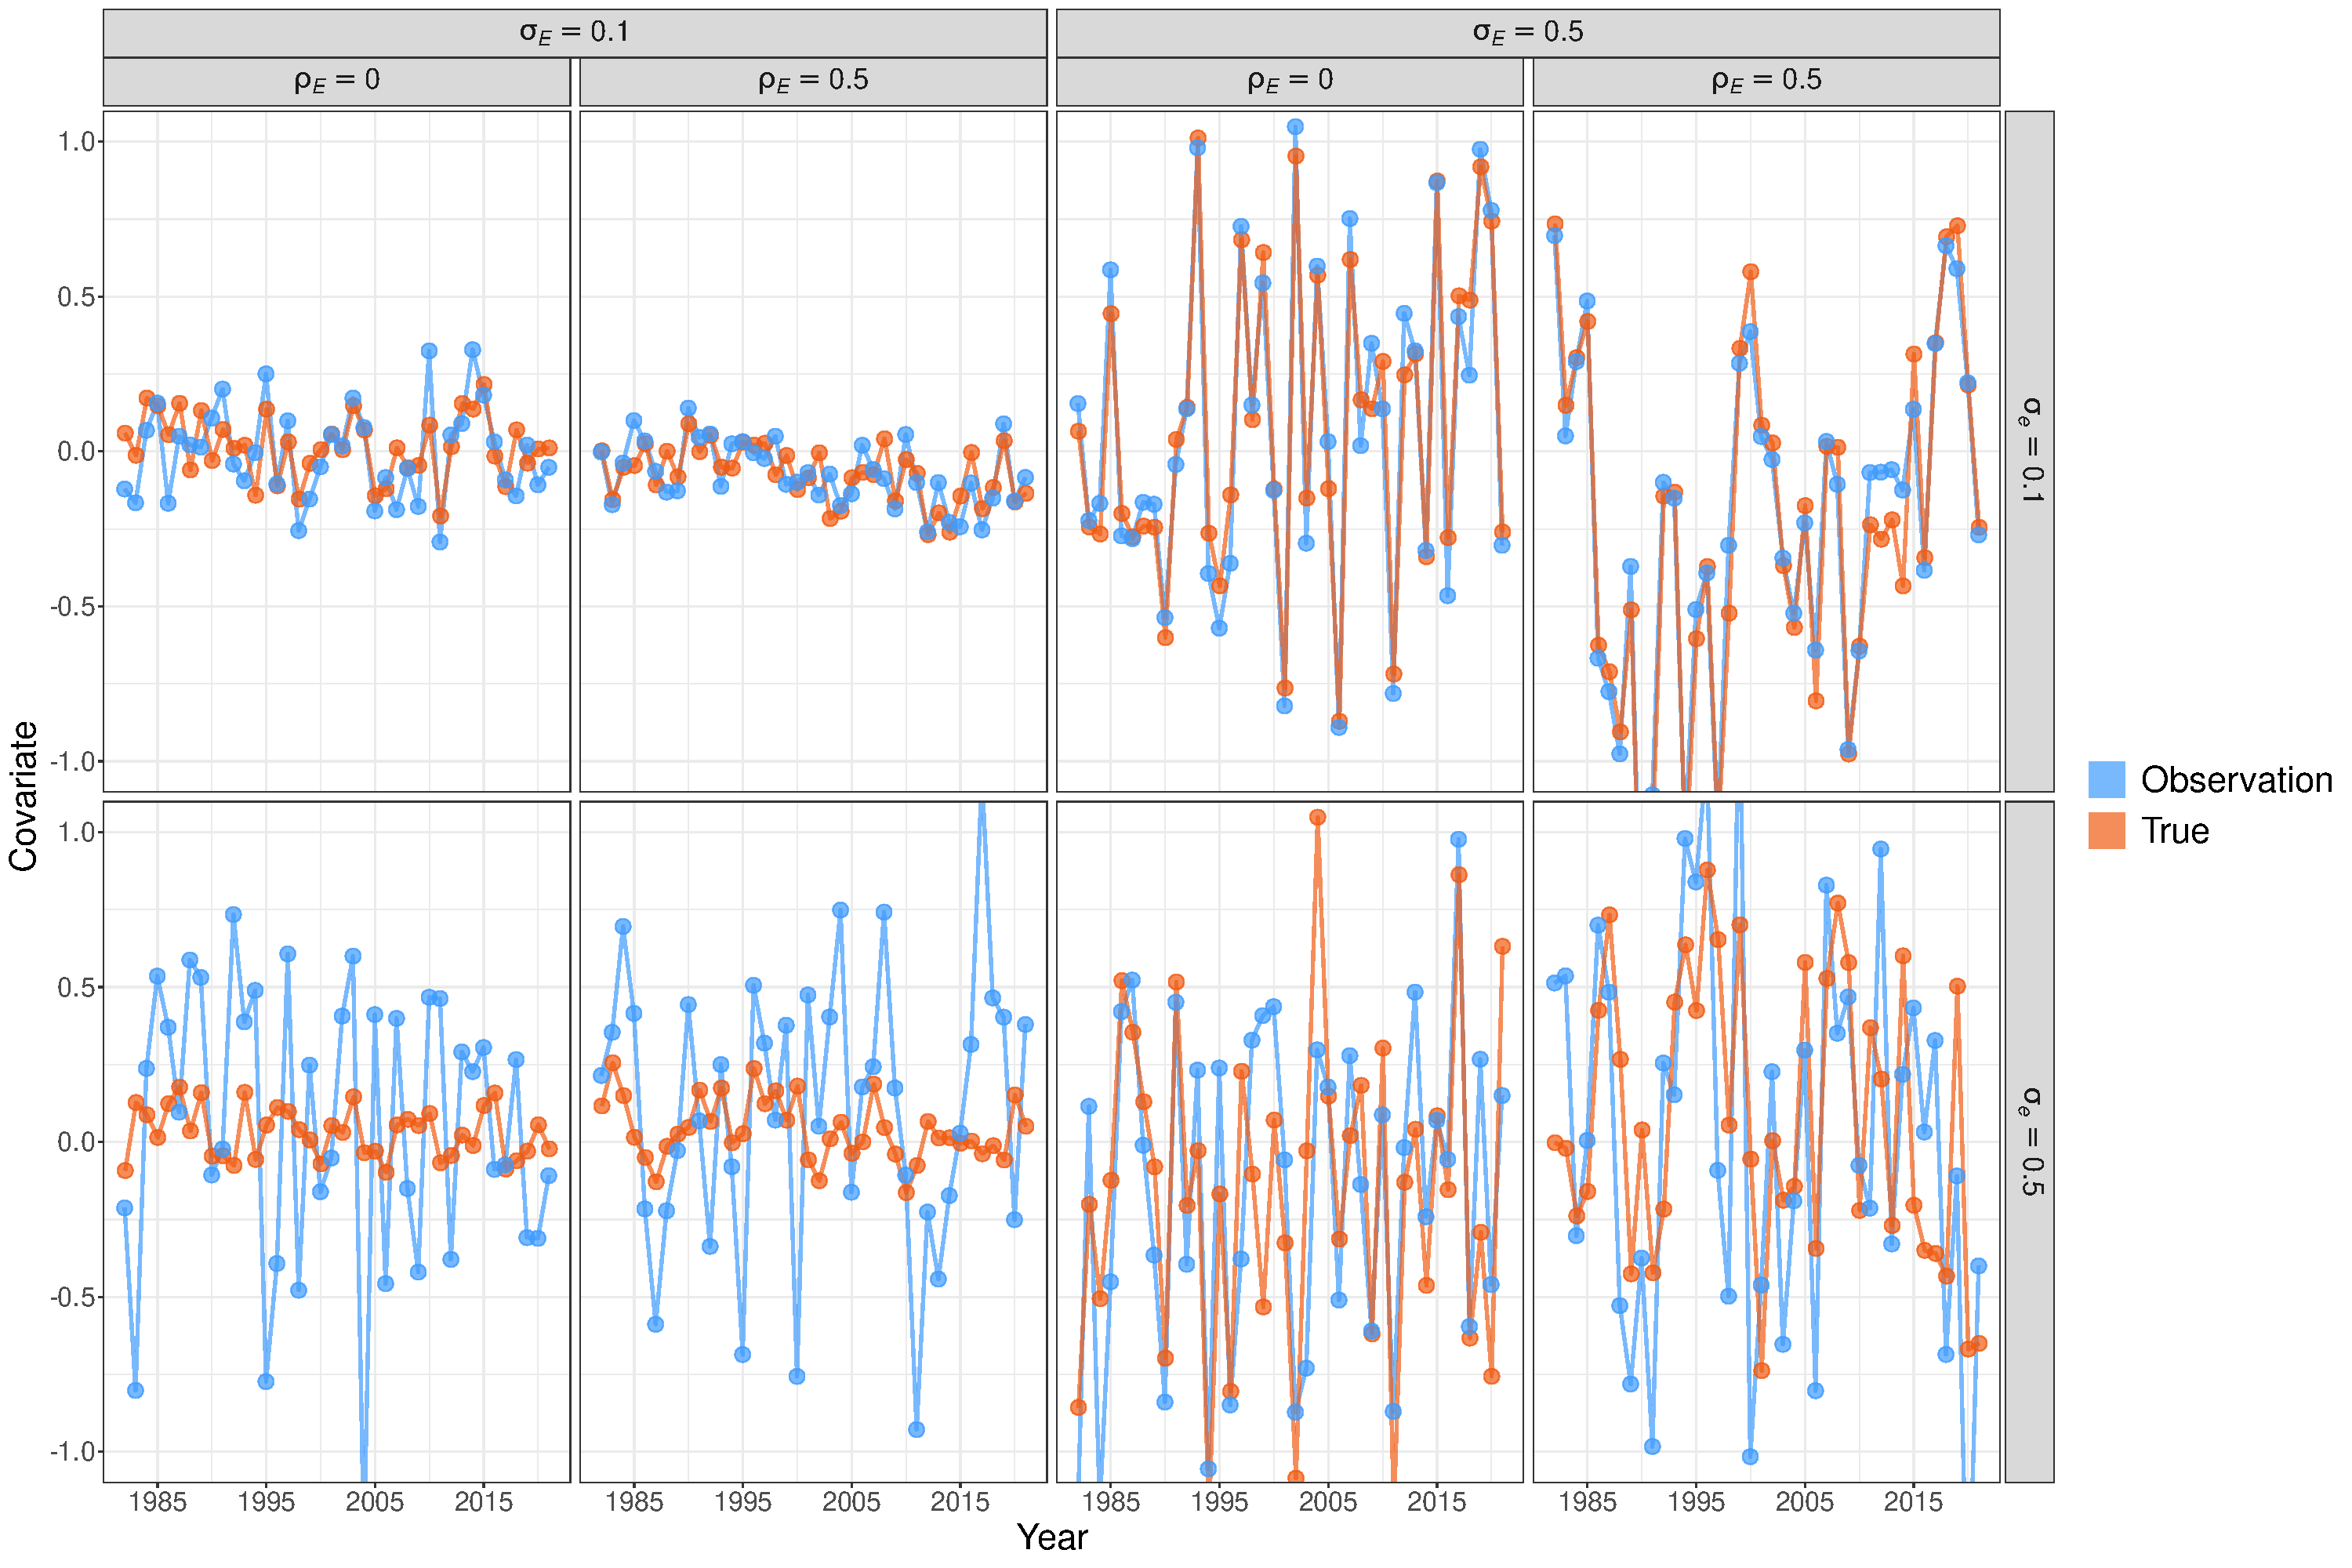
\includegraphics[height = \textheight]{Ecov_true_obs_example}
%DIFDELCMD < \end{center}
%DIFDELCMD < %%%
%DIFDELCMD < \caption{%
{%DIFAUXCMD
\DIFdelFL{Example simulations of environmental covariate latent processes and observations with different levels of observation error, and different assumptions about variability of the latent process.}}%DIFAUXCMD
%DIFDELCMD < \label{om_ecov_example}
%DIFDELCMD < \end{figure}
%DIFDELCMD < \end{landscape}
%DIFDELCMD < 

%DIFDELCMD < \begin{figure}
%DIFDELCMD < \begin{center}
%DIFDELCMD < 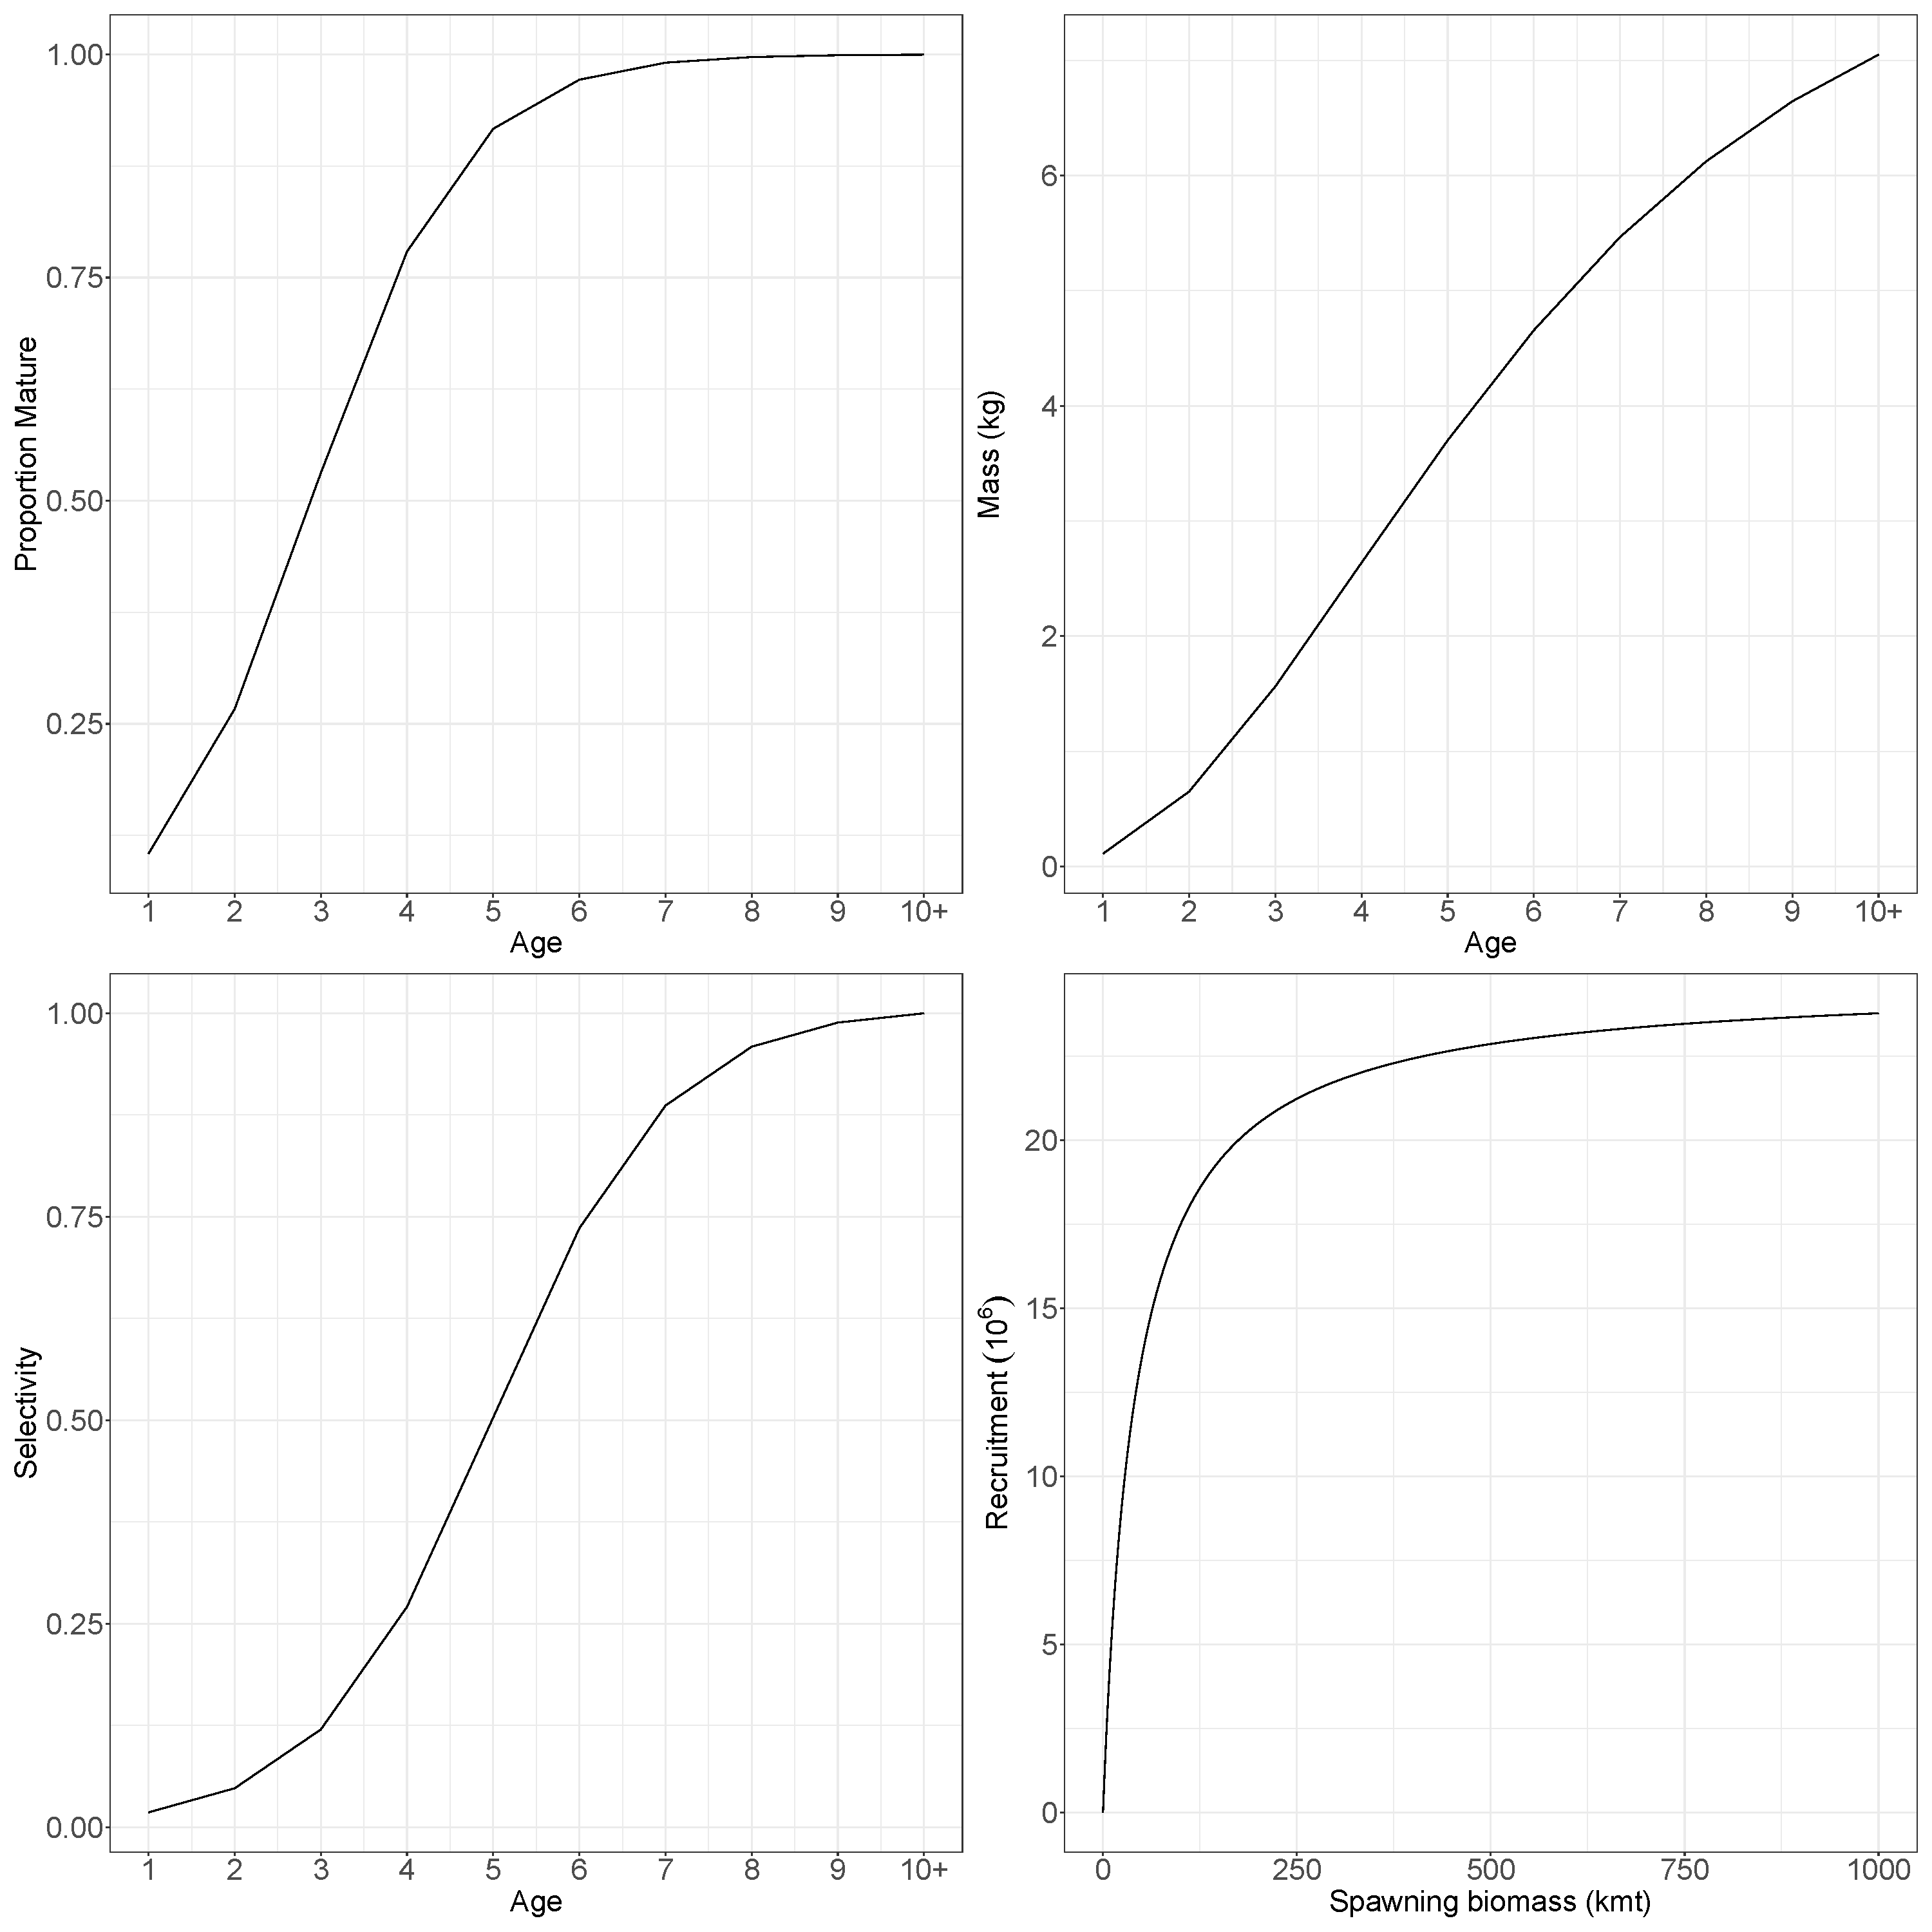
\includegraphics[width = \textwidth]{om_input_plots_figure}
%DIFDELCMD < \end{center}
%DIFDELCMD < %%%
%DIFDELCMD < \caption{%
{%DIFAUXCMD
\DIFdelFL{The proportion mature at age, weight at age, fleet and index selectivity at age, and Beverton-Holt stock-recruit relationship assumed for the population in all OMs. For OMs with random effects on fleet selectivity, this represents the selectivity at the mean of the random effects.}}%DIFAUXCMD
%DIFDELCMD < \label{om_inputs_fig}
%DIFDELCMD < \end{figure}
%DIFDELCMD < 

%DIFDELCMD < \begin{landscape}
%DIFDELCMD < \begin{figure}
%DIFDELCMD < \begin{center}
%DIFDELCMD < 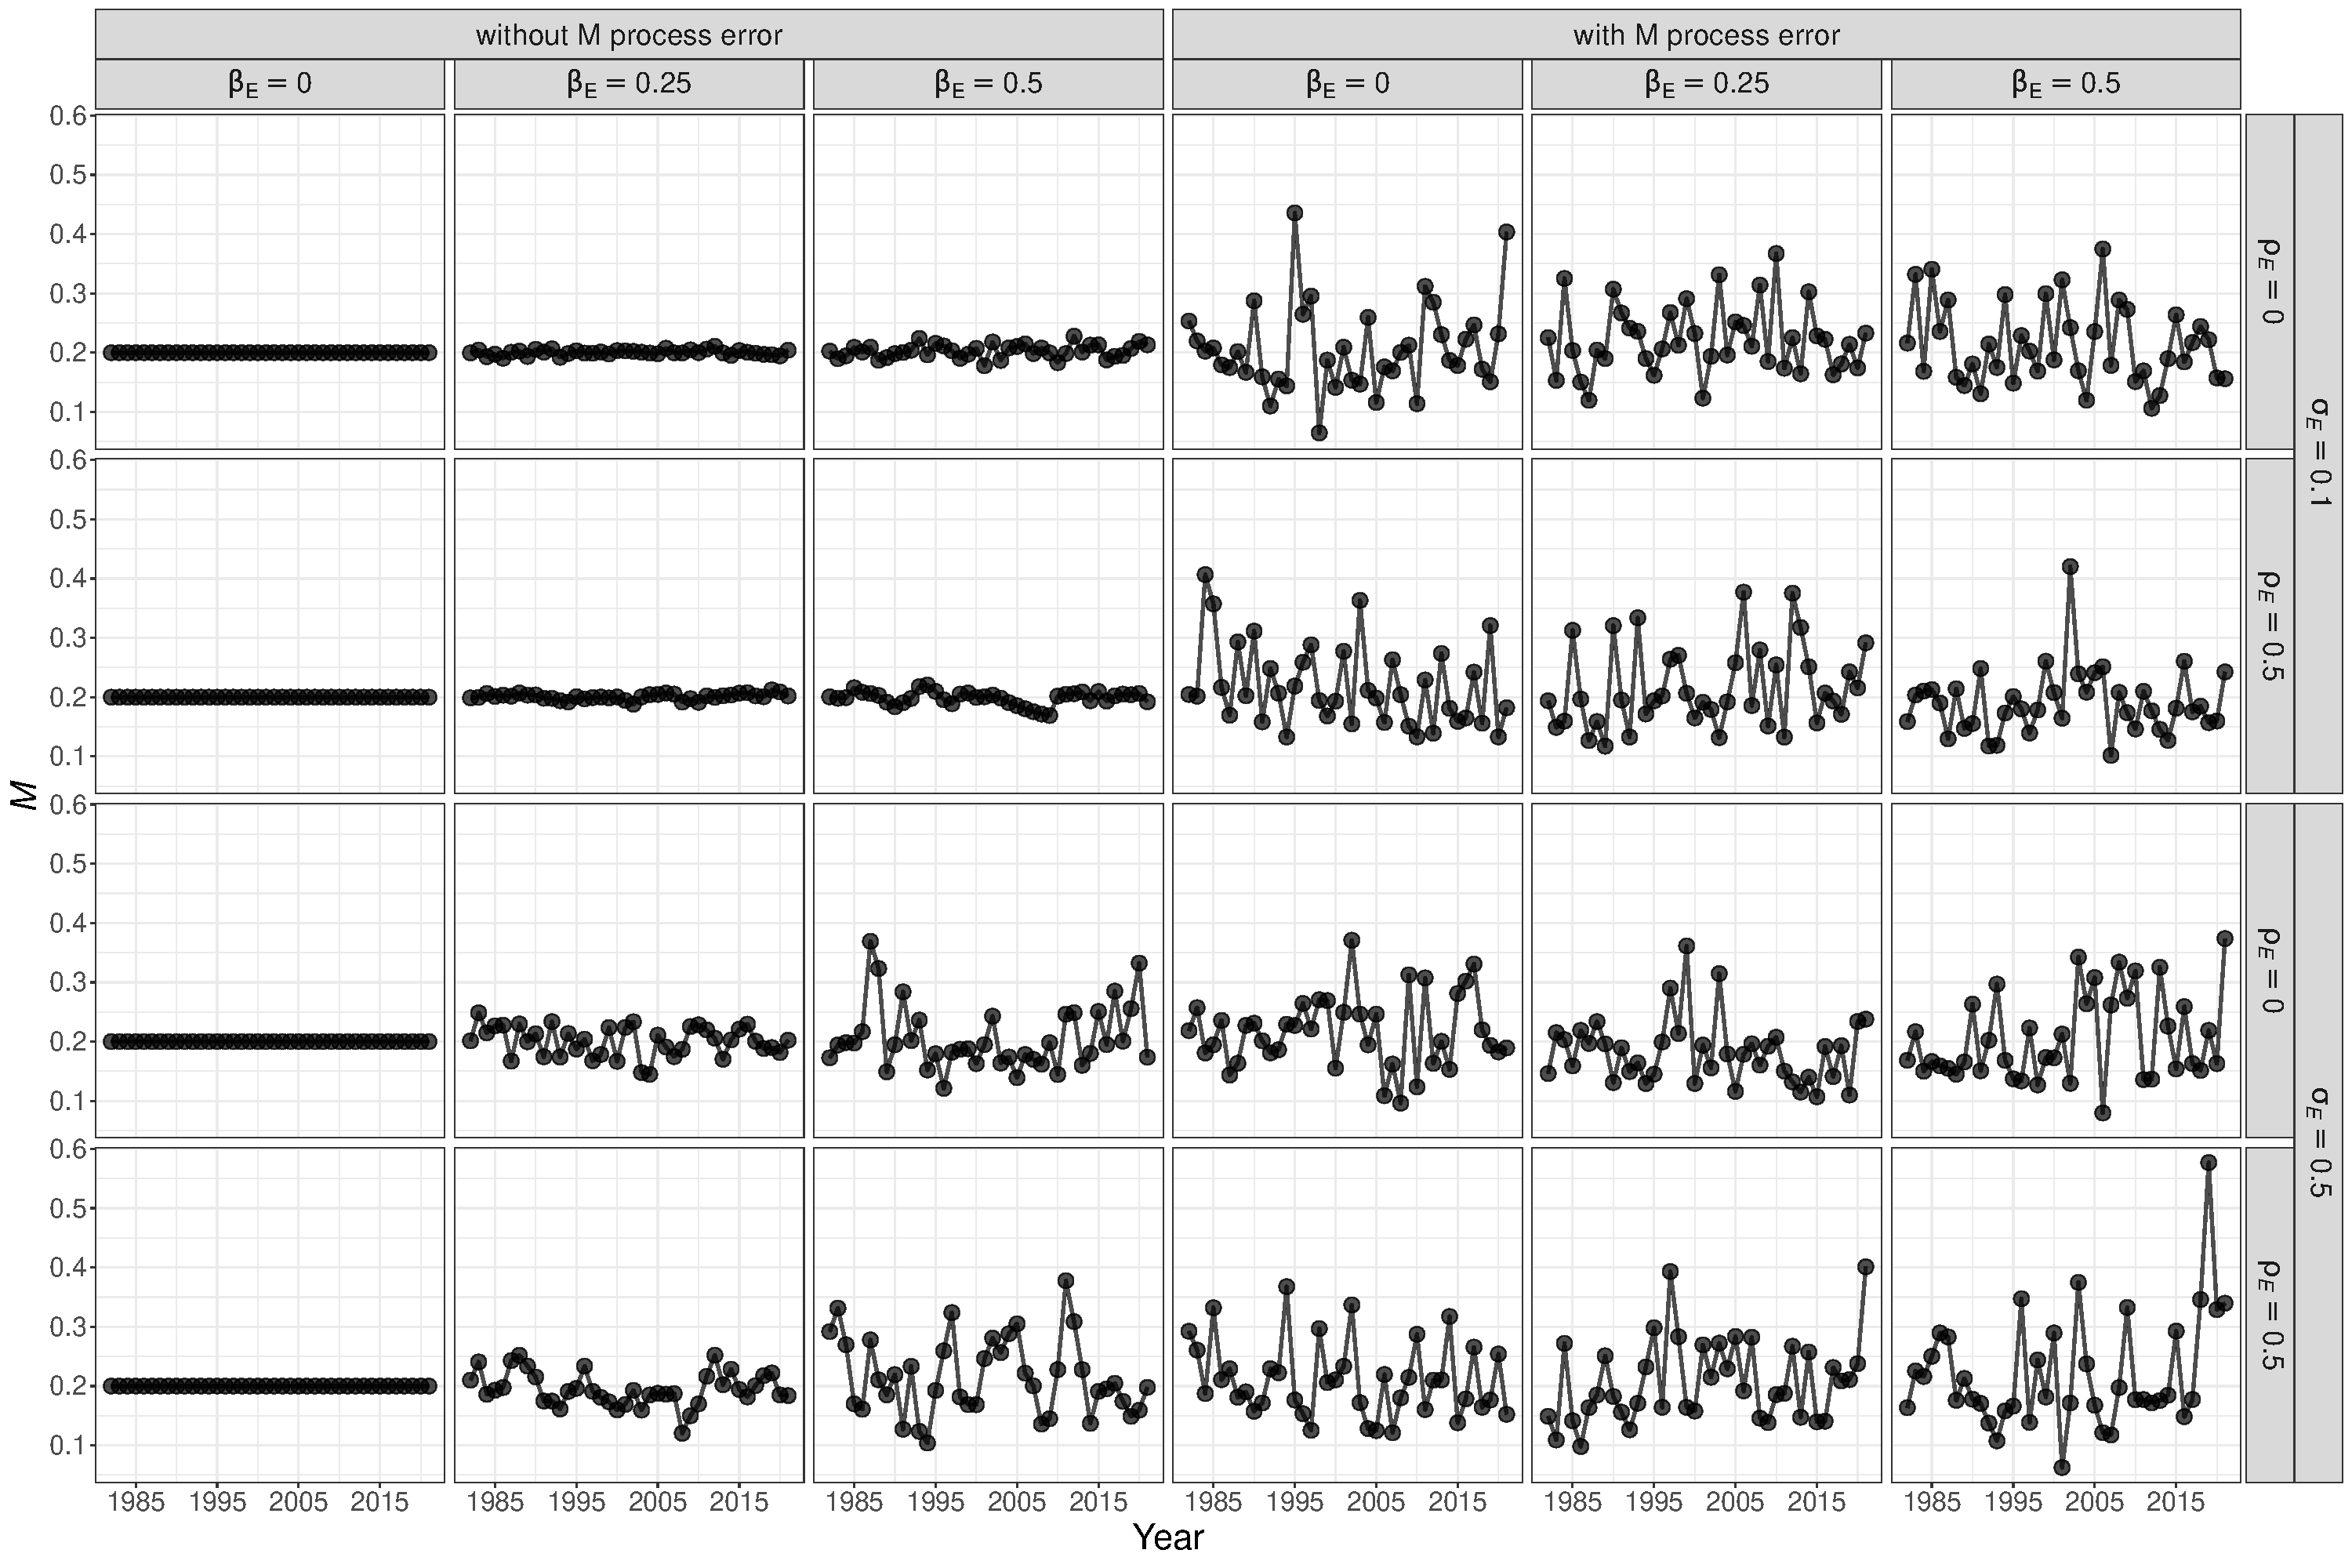
\includegraphics[height = \textheight]{M_example}
%DIFDELCMD < \end{center}
%DIFDELCMD < %%%
%DIFDELCMD < \caption{%
{%DIFAUXCMD
\DIFdelFL{Example simulations of annual $M$ that may be a function of a temporally varying environmental covariate and autoregressive random effects.}}%DIFAUXCMD
%DIFDELCMD < \label{M_example}
%DIFDELCMD < \end{figure}
%DIFDELCMD < \end{landscape}
%DIFDELCMD < 

%DIFDELCMD < \begin{landscape}
%DIFDELCMD < \begin{figure}
%DIFDELCMD < \begin{center}
%DIFDELCMD < 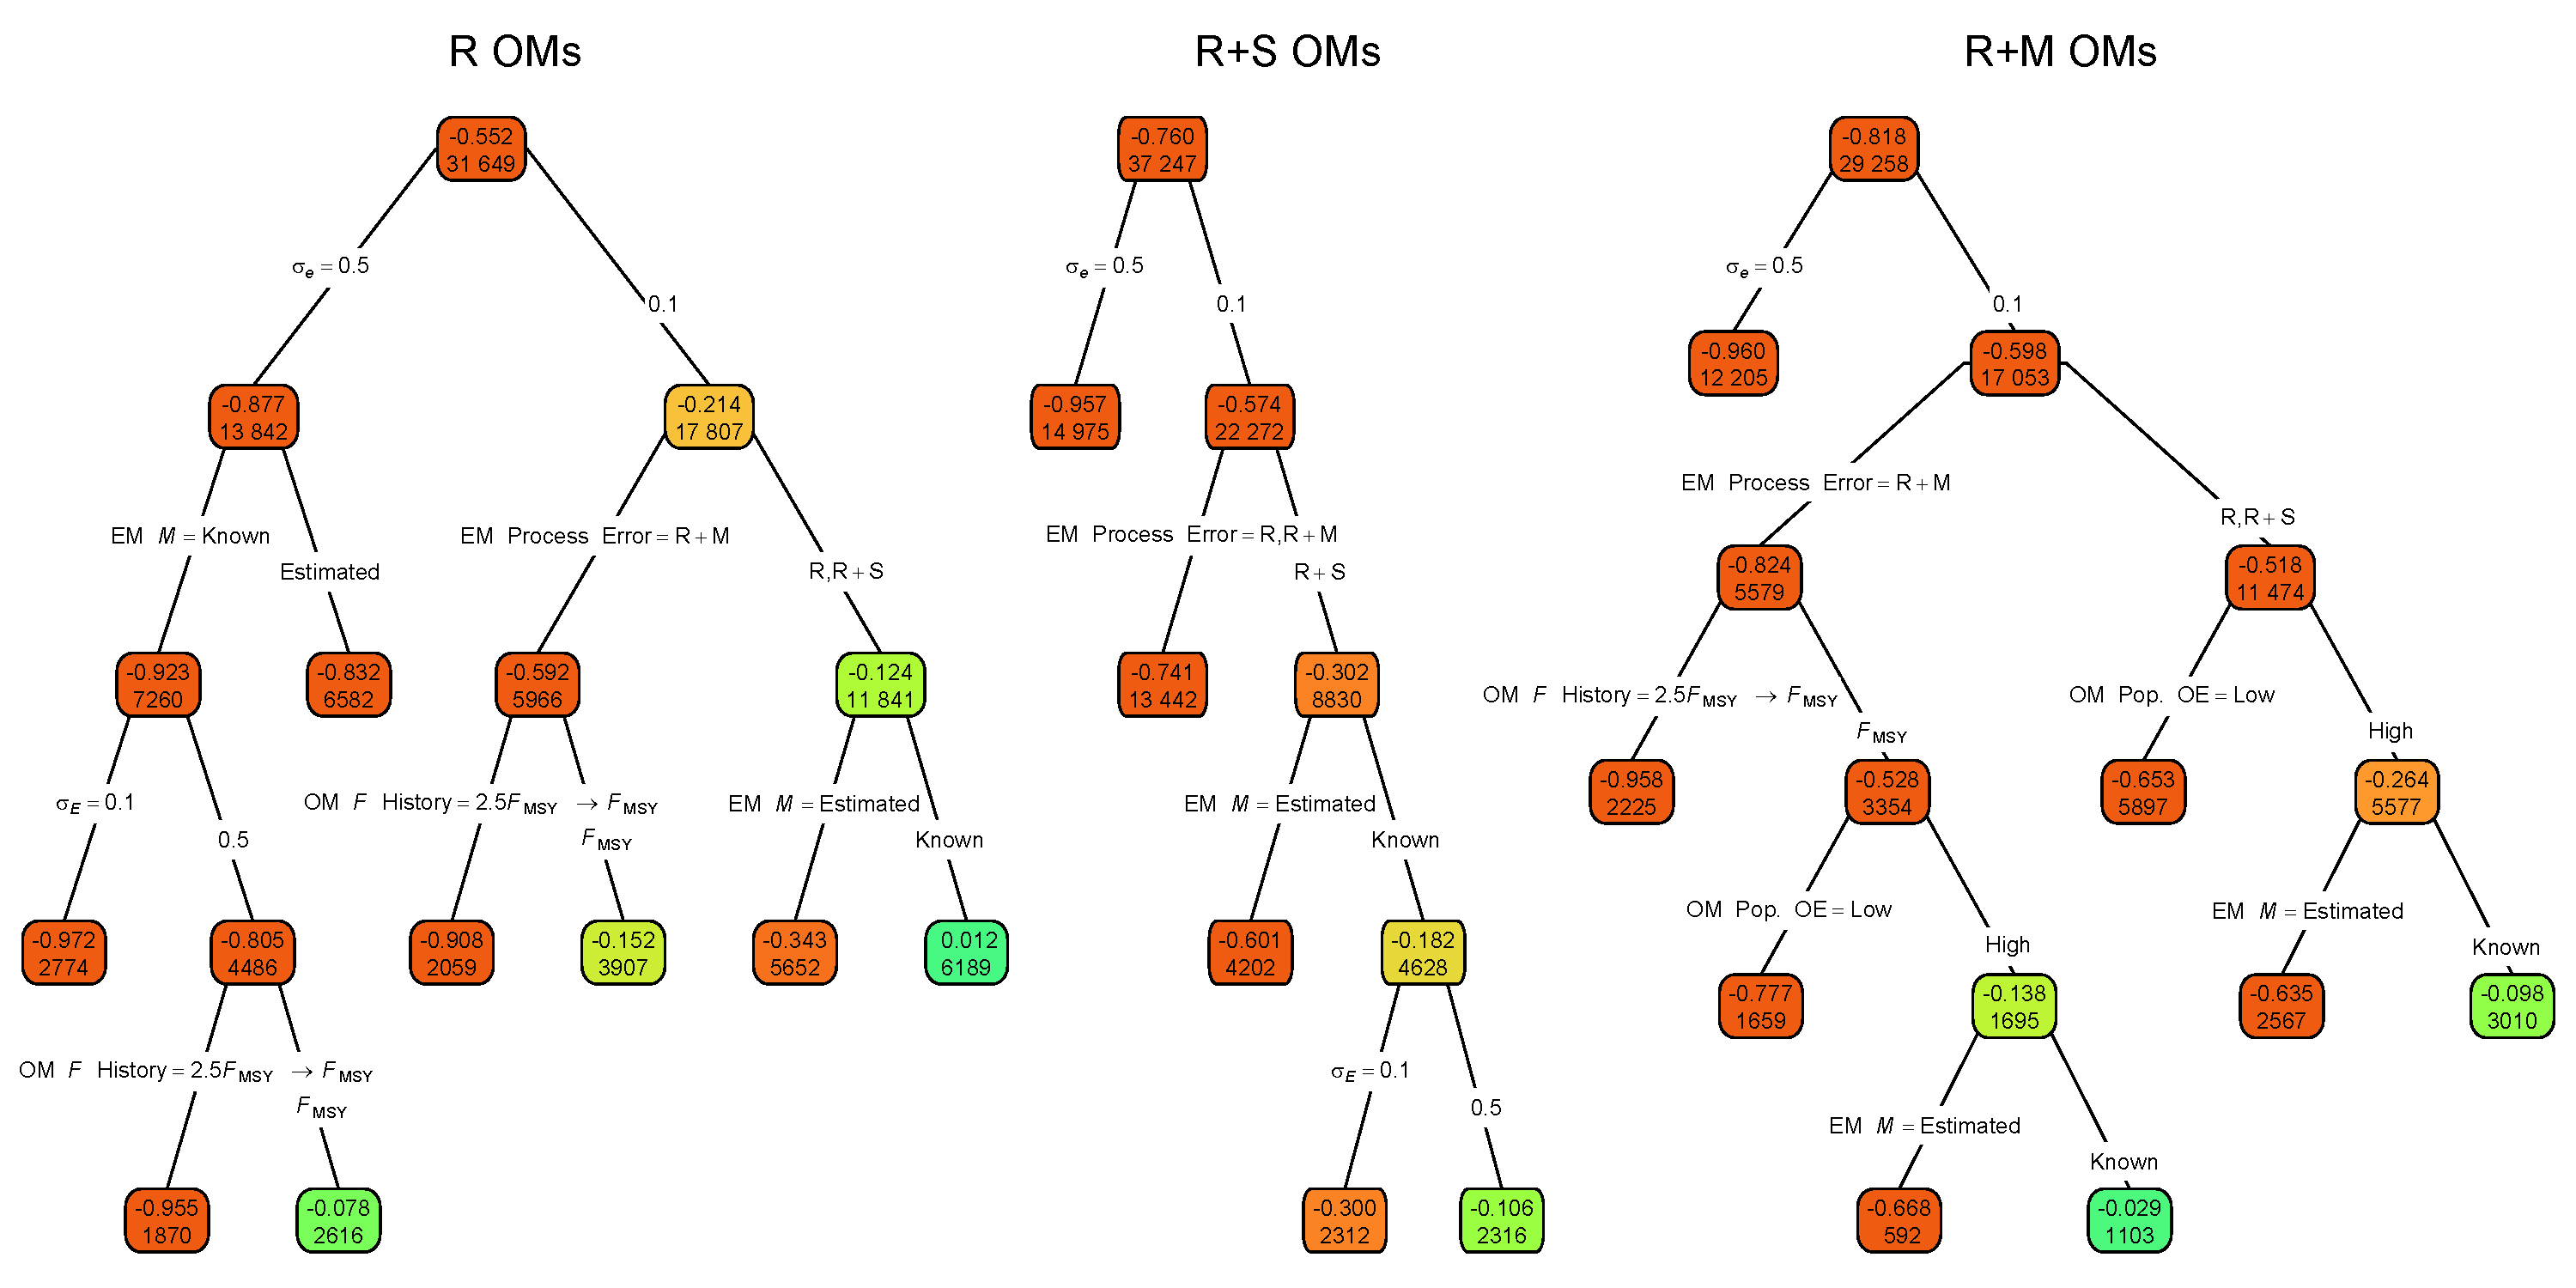
\includegraphics[width = 1.4\textwidth]{ecov_beta_SE_bias_regtree_plots}
%DIFDELCMD < \end{center}
%DIFDELCMD < %%%
%DIFDELCMD < \caption{%
{%DIFAUXCMD
\DIFdelFL{Regression trees indicating primary factors determining reductions in sums of squares of errors in estimation of the Hessian-based standard error estimates for covariate effect on $M$ ($\widehat {\text{SE}}\left(\widehat \beta_E\right)$) for operating models (OMs) with process error on recruitment only (R), recruitment and apparent survival (R+S), or recruitment and natural mortality (R+M). Each node shows the median error (top) and number of observations (bottom) for the corresponding subset. Lower or higher median absolute errors of the process error assumption are indicated by more green or red polygons, respectively.}}%DIFAUXCMD
%DIFDELCMD < \label{ecov_effect_SE_bias_regtree}
%DIFDELCMD < \end{figure}
%DIFDELCMD < \end{landscape}
%DIFDELCMD < 

%DIFDELCMD < \begin{landscape}
%DIFDELCMD < \begin{figure}
%DIFDELCMD < \begin{center}
%DIFDELCMD < 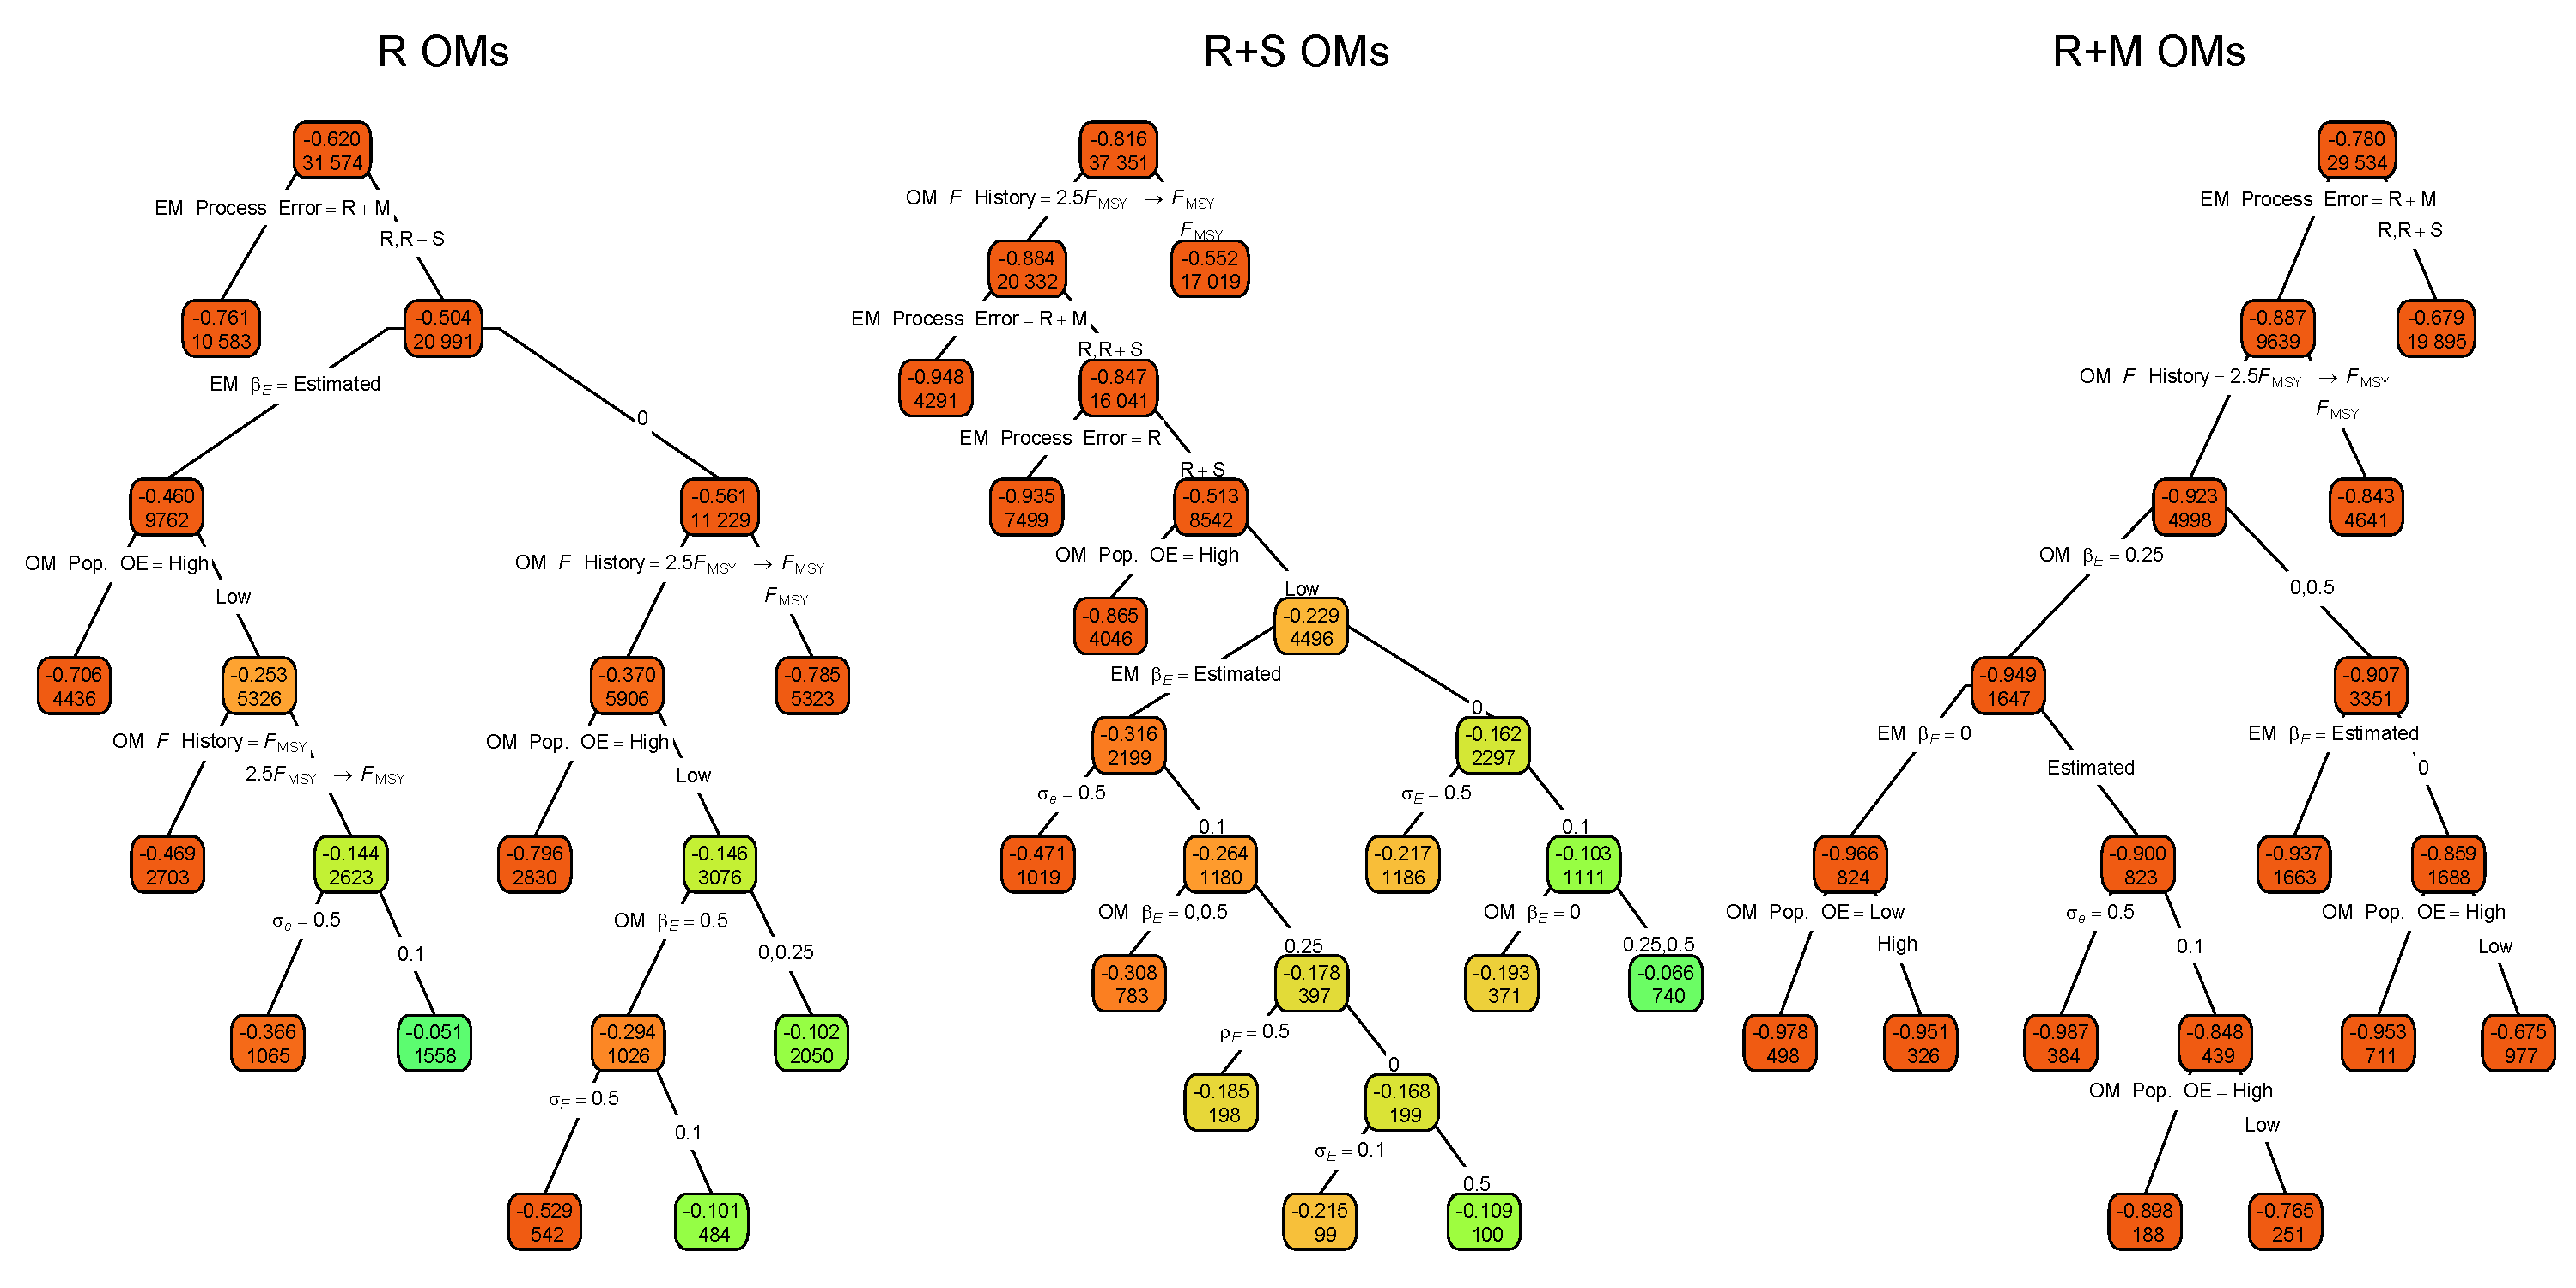
\includegraphics[width = 1.4\textwidth]{median_M_SE_bias_regtree_plots}
%DIFDELCMD < \end{center}
%DIFDELCMD < %%%
%DIFDELCMD < \caption{%
{%DIFAUXCMD
\DIFdelFL{Regression trees indicating primary factors determining reductions in sums of squares of errors in estimation of the Hessian-based standard error estimates for median $M$ parameter ($\widehat {\text{SE}}\left(\widehat \beta_M\right)$) in EMs fitted to operating models (OMs) with process error on recruitment only (R), recruitment and apparent survival (R+S), or recruitment and natural mortality (R+M). Each node shows the median error (top) and number of observations (bottom) for the corresponding subset. Lower or higher median absolute errors of the process error assumption are indicated by more green or red polygons, respectively.}}%DIFAUXCMD
%DIFDELCMD < \label{med_M_SE_bias_regtree}
%DIFDELCMD < \end{figure}
%DIFDELCMD < \end{landscape}
%DIFDELCMD < 

%DIFDELCMD < \begin{landscape}
%DIFDELCMD < \begin{figure}
%DIFDELCMD < \begin{center}
%DIFDELCMD < 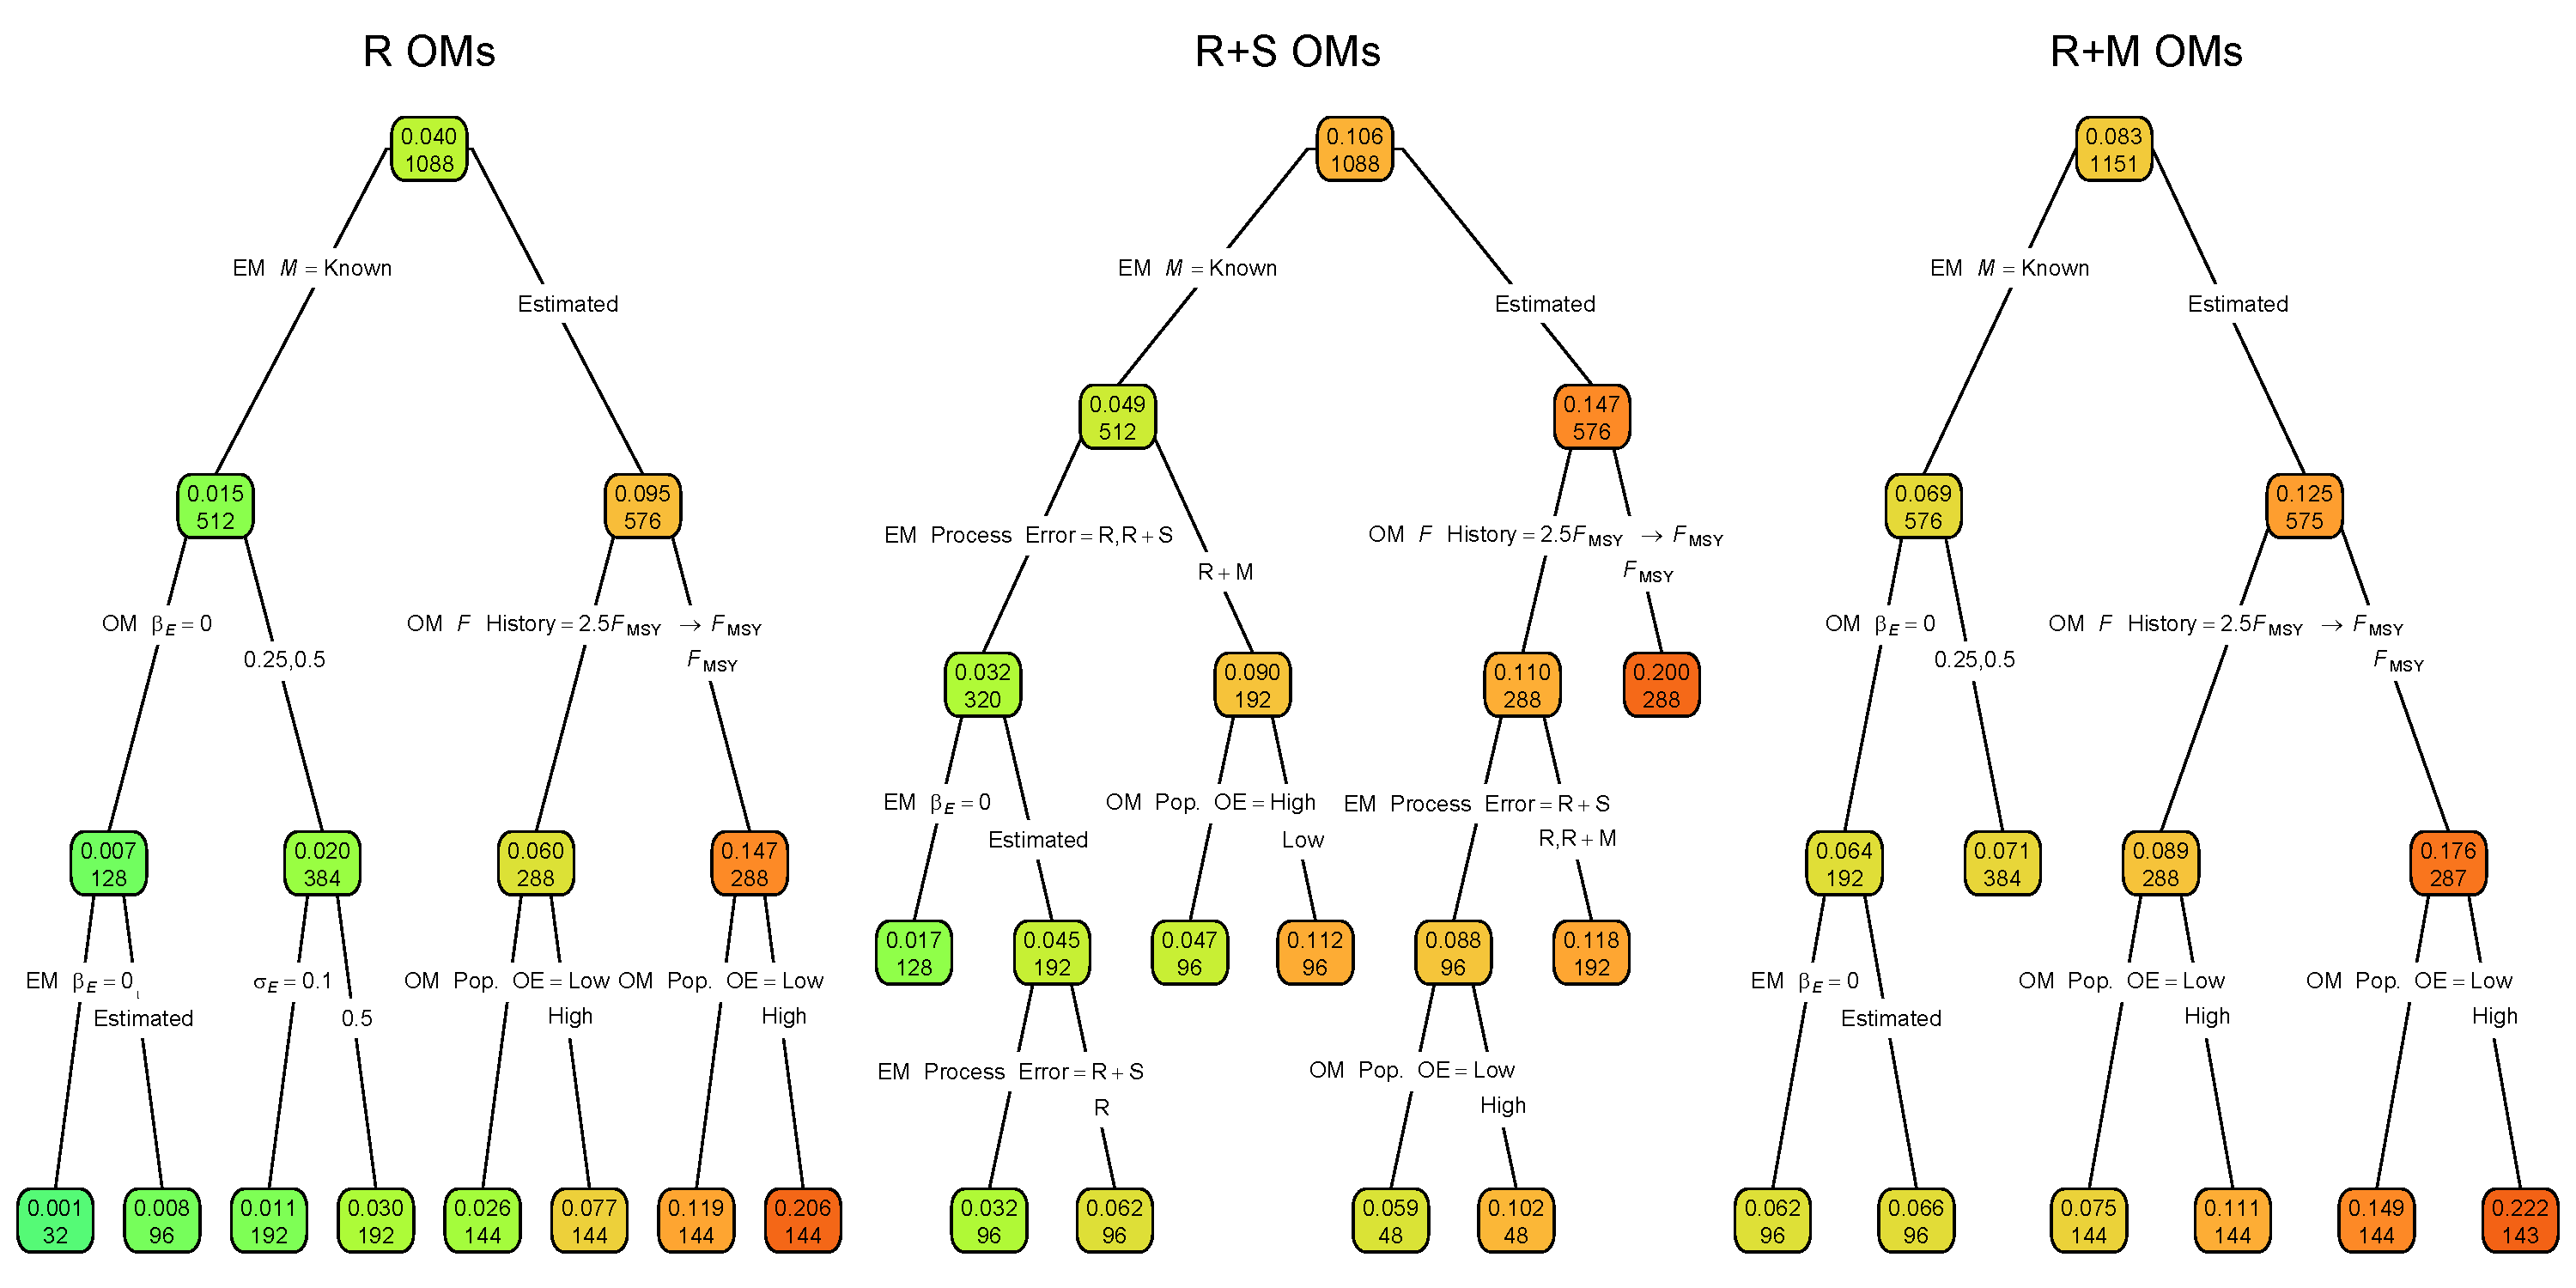
\includegraphics[width = 1.4\textwidth]{term_M_rmse_regtree_plots}
%DIFDELCMD < \end{center}
%DIFDELCMD < %%%
%DIFDELCMD < \caption{%
{%DIFAUXCMD
\DIFdelFL{Regression trees indicating primary factors determining reductions in sums of squares for the log-transformed RMSE of terminal year $M$ in EMs fitted to operating models (OMs) with process error on recruitment only (R), recruitment and apparent survival (R+S), or recruitment and natural mortality (R+M). Each node shows the median error (top) and number of observations (bottom) for the corresponding subset. Lower or higher median RMSE are indicated by more red or green polygons, respectively.}}%DIFAUXCMD
%DIFDELCMD < \label{term_M_rmse_regtree}
%DIFDELCMD < \end{figure}
%DIFDELCMD < \end{landscape}
%DIFDELCMD < 

%DIFDELCMD < \begin{landscape}
%DIFDELCMD < \begin{figure}
%DIFDELCMD < \begin{center}
%DIFDELCMD < 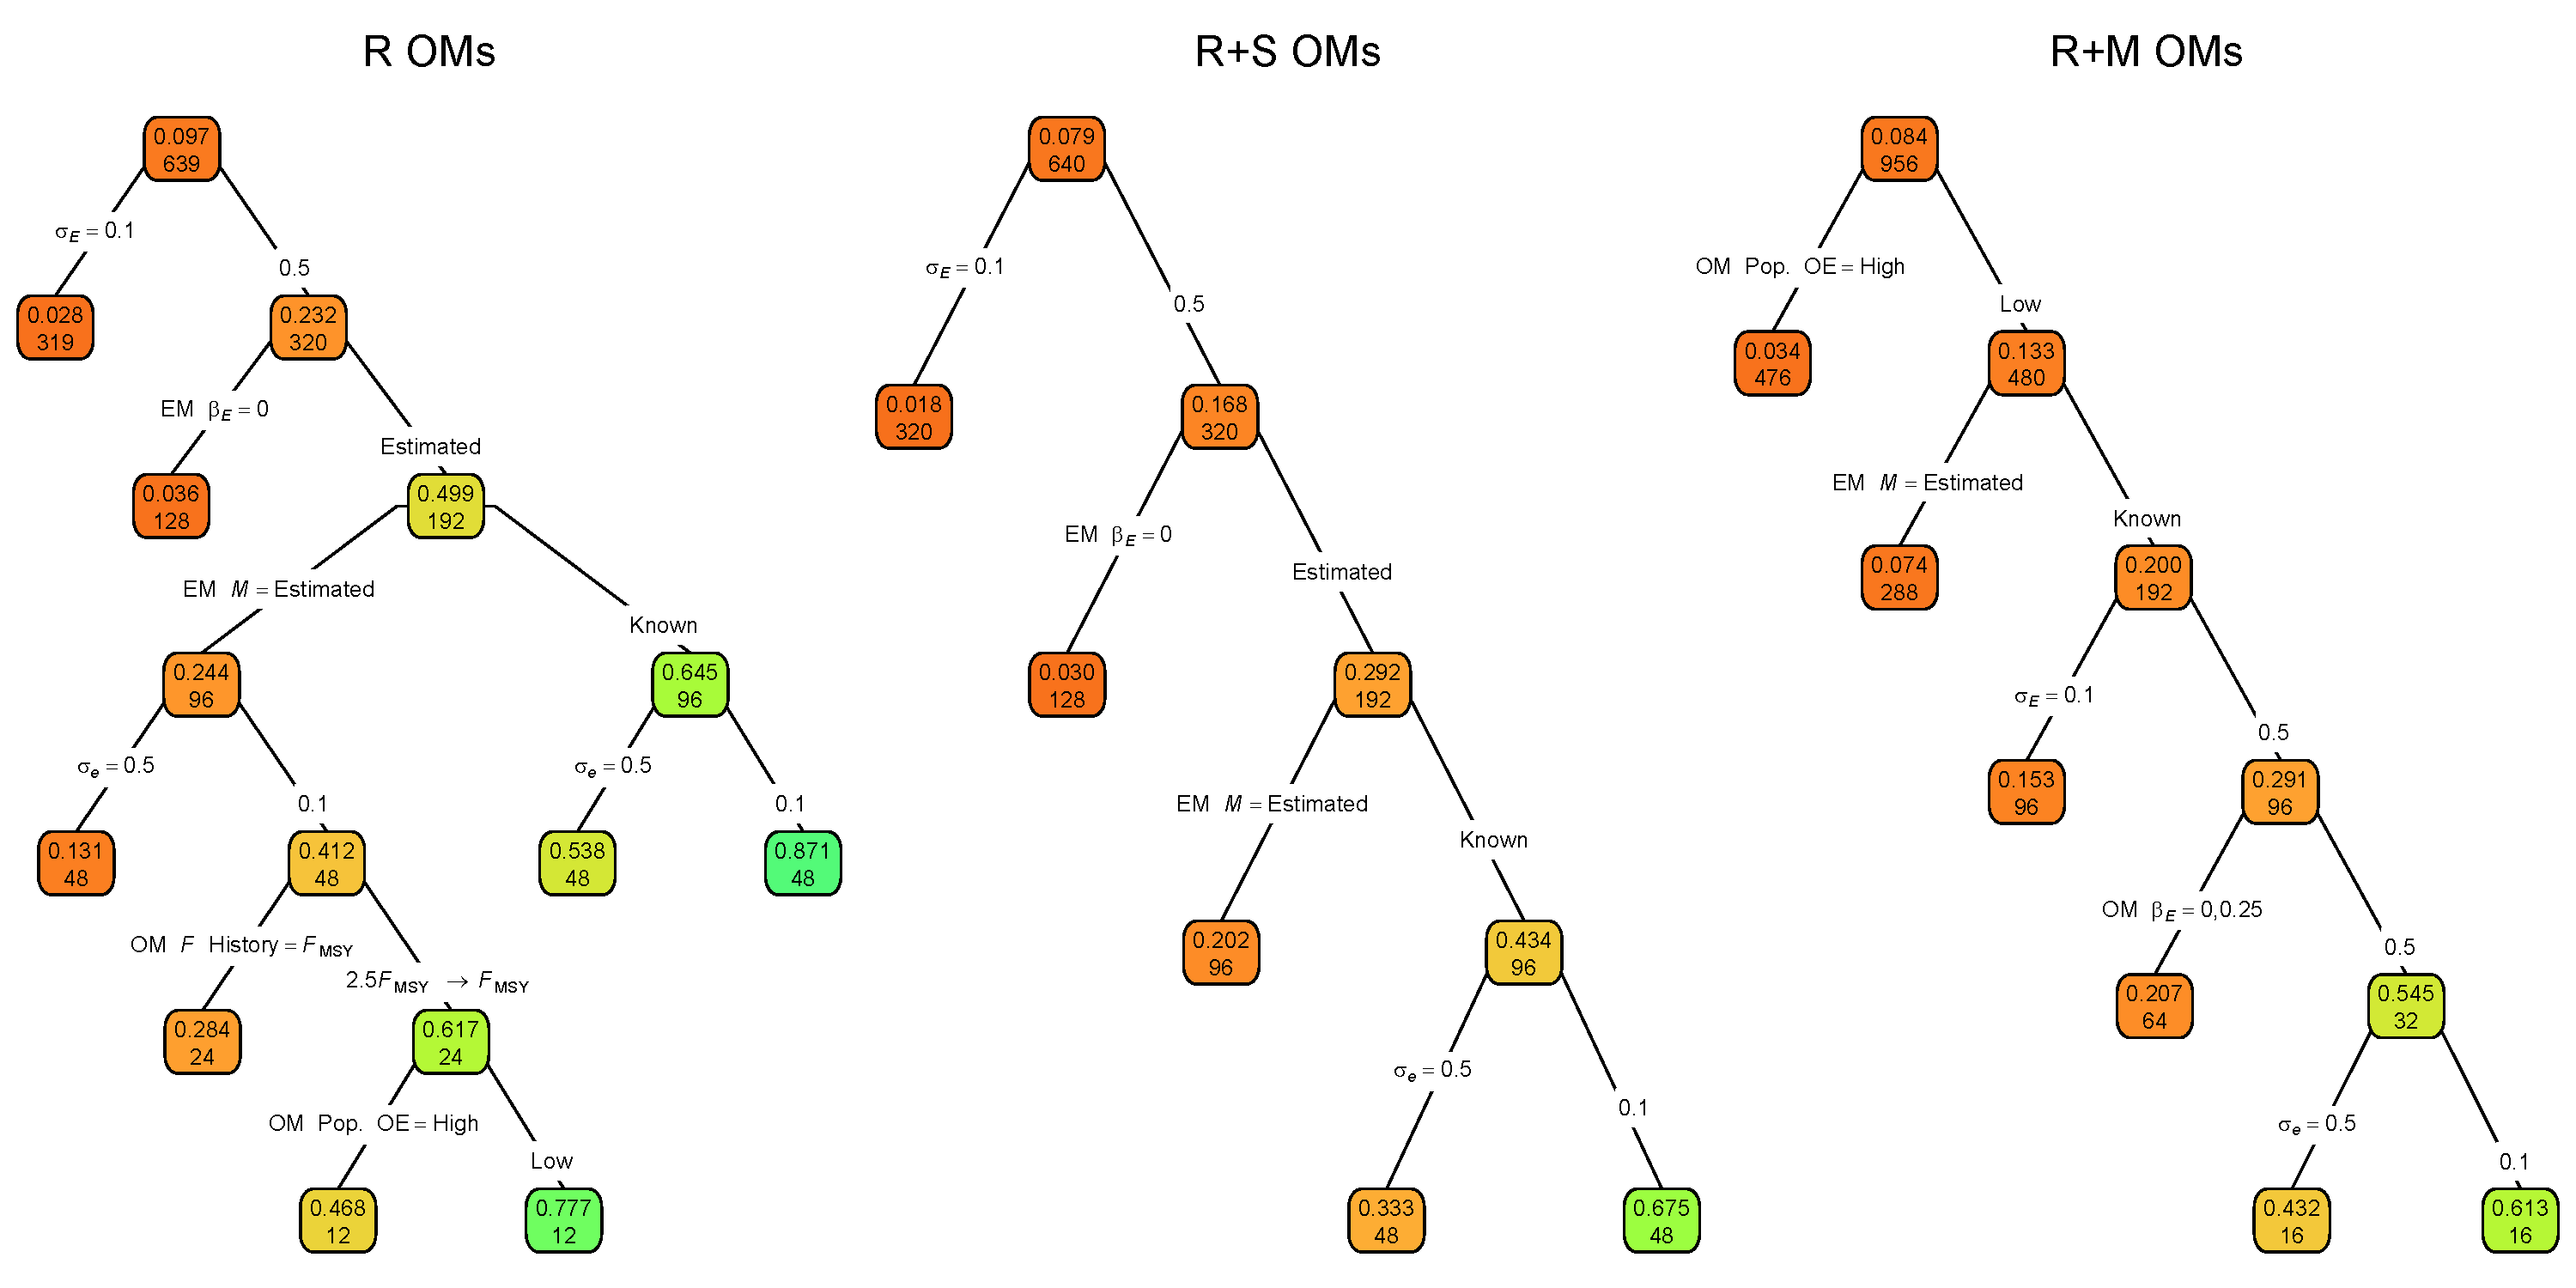
\includegraphics[width = 1.4\textwidth]{term_M_corr_regtree_plots}
%DIFDELCMD < \end{center}
%DIFDELCMD < %%%
%DIFDELCMD < \caption{%
{%DIFAUXCMD
\DIFdelFL{Regression trees indicating primary factors determining reductions in sums of squares for the correlation of terminal year $M$ estimates and true values in EMs fitted to operating models (OMs) with process error on recruitment only (R), recruitment and apparent survival (R+S), or recruitment and natural mortality (R+M). Each node shows the median error (top) and number of observations (bottom) for the corresponding subset. Lower or higher median correlations are indicated by more red or green polygons, respectively.}}%DIFAUXCMD
%DIFDELCMD < \label{term_M_corr_regtree}
%DIFDELCMD < \end{figure}
%DIFDELCMD < \end{landscape}
%DIFDELCMD < 

%DIFDELCMD < \begin{landscape}
%DIFDELCMD < \begin{figure}
%DIFDELCMD < \begin{center}
%DIFDELCMD < 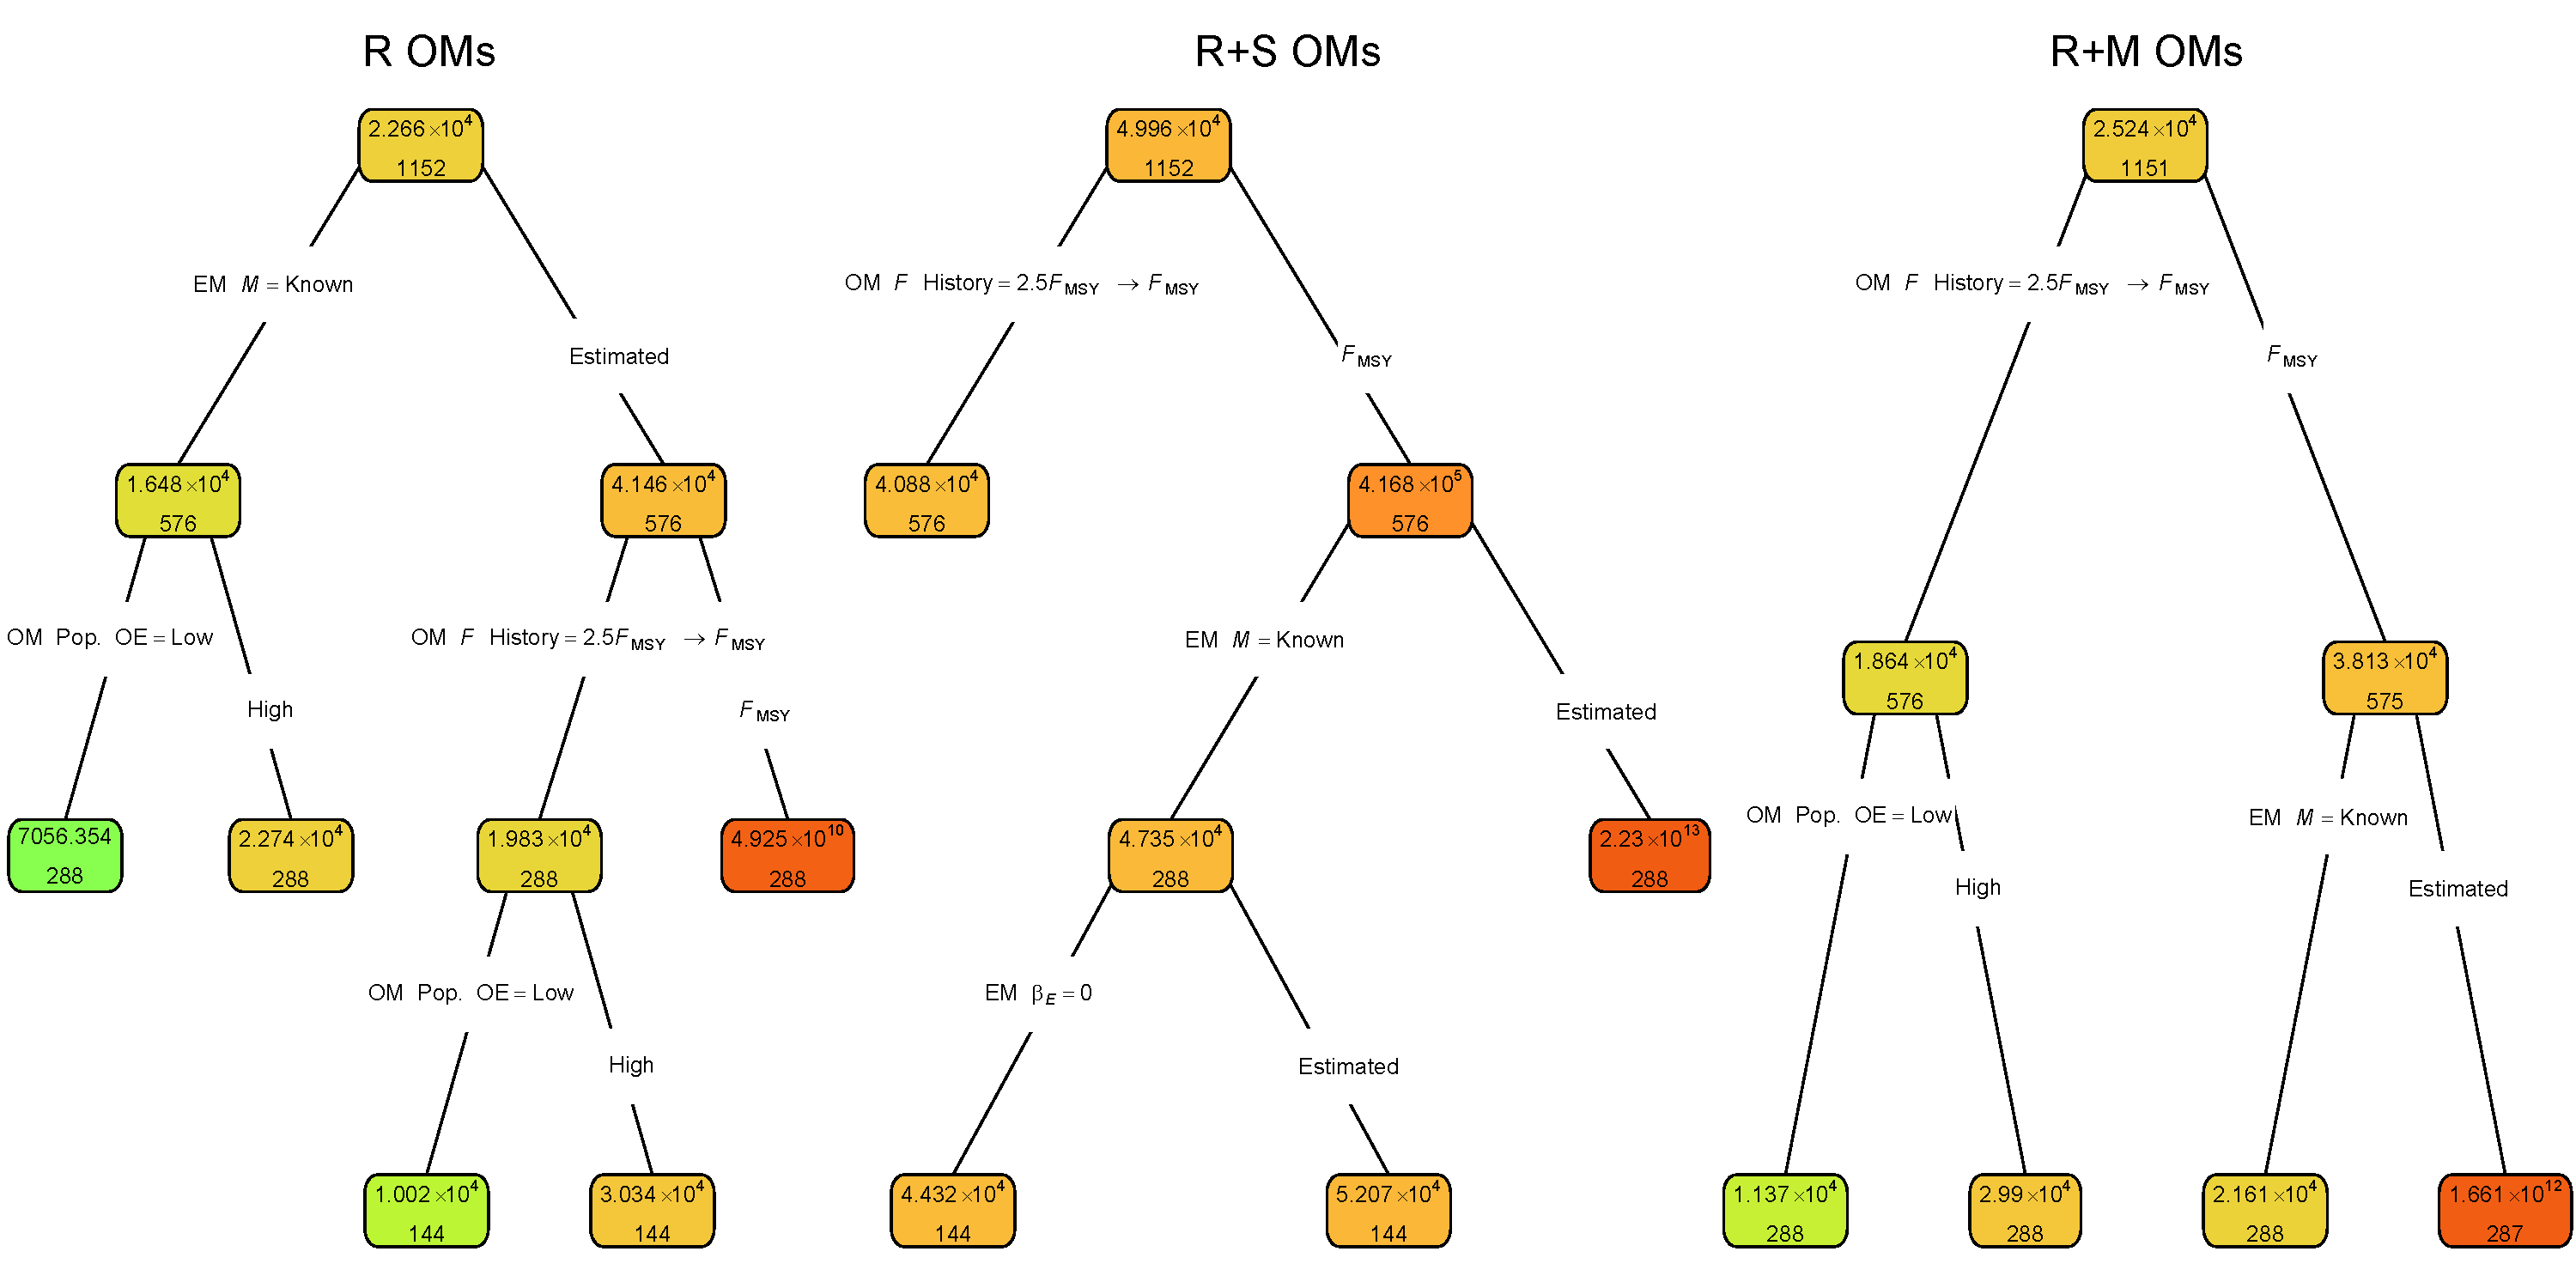
\includegraphics[width = 1.4\textwidth]{term_SSB_rmse_regtree_plots}
%DIFDELCMD < \end{center}
%DIFDELCMD < %%%
%DIFDELCMD < \caption{%
{%DIFAUXCMD
\DIFdelFL{Regression trees indicating primary factors determining reductions in sums of squares for the log-transformed RMSE of terminal year SSB in EMs fitted to operating models (OMs) with process error on recruitment only (R), recruitment and apparent survival (R+S), or recruitment and natural mortality (R+M). Each node shows the median error (top) and number of observations (bottom) for the corresponding subset. Lower or higher median RMSE are indicated by more red or green polygons, respectively.}}%DIFAUXCMD
%DIFDELCMD < \label{term_SSB_rmse_regtree}
%DIFDELCMD < \end{figure}
%DIFDELCMD < \end{landscape}
%DIFDELCMD < 

%DIFDELCMD < \begin{landscape}
%DIFDELCMD < \begin{figure}
%DIFDELCMD < \begin{center}
%DIFDELCMD < 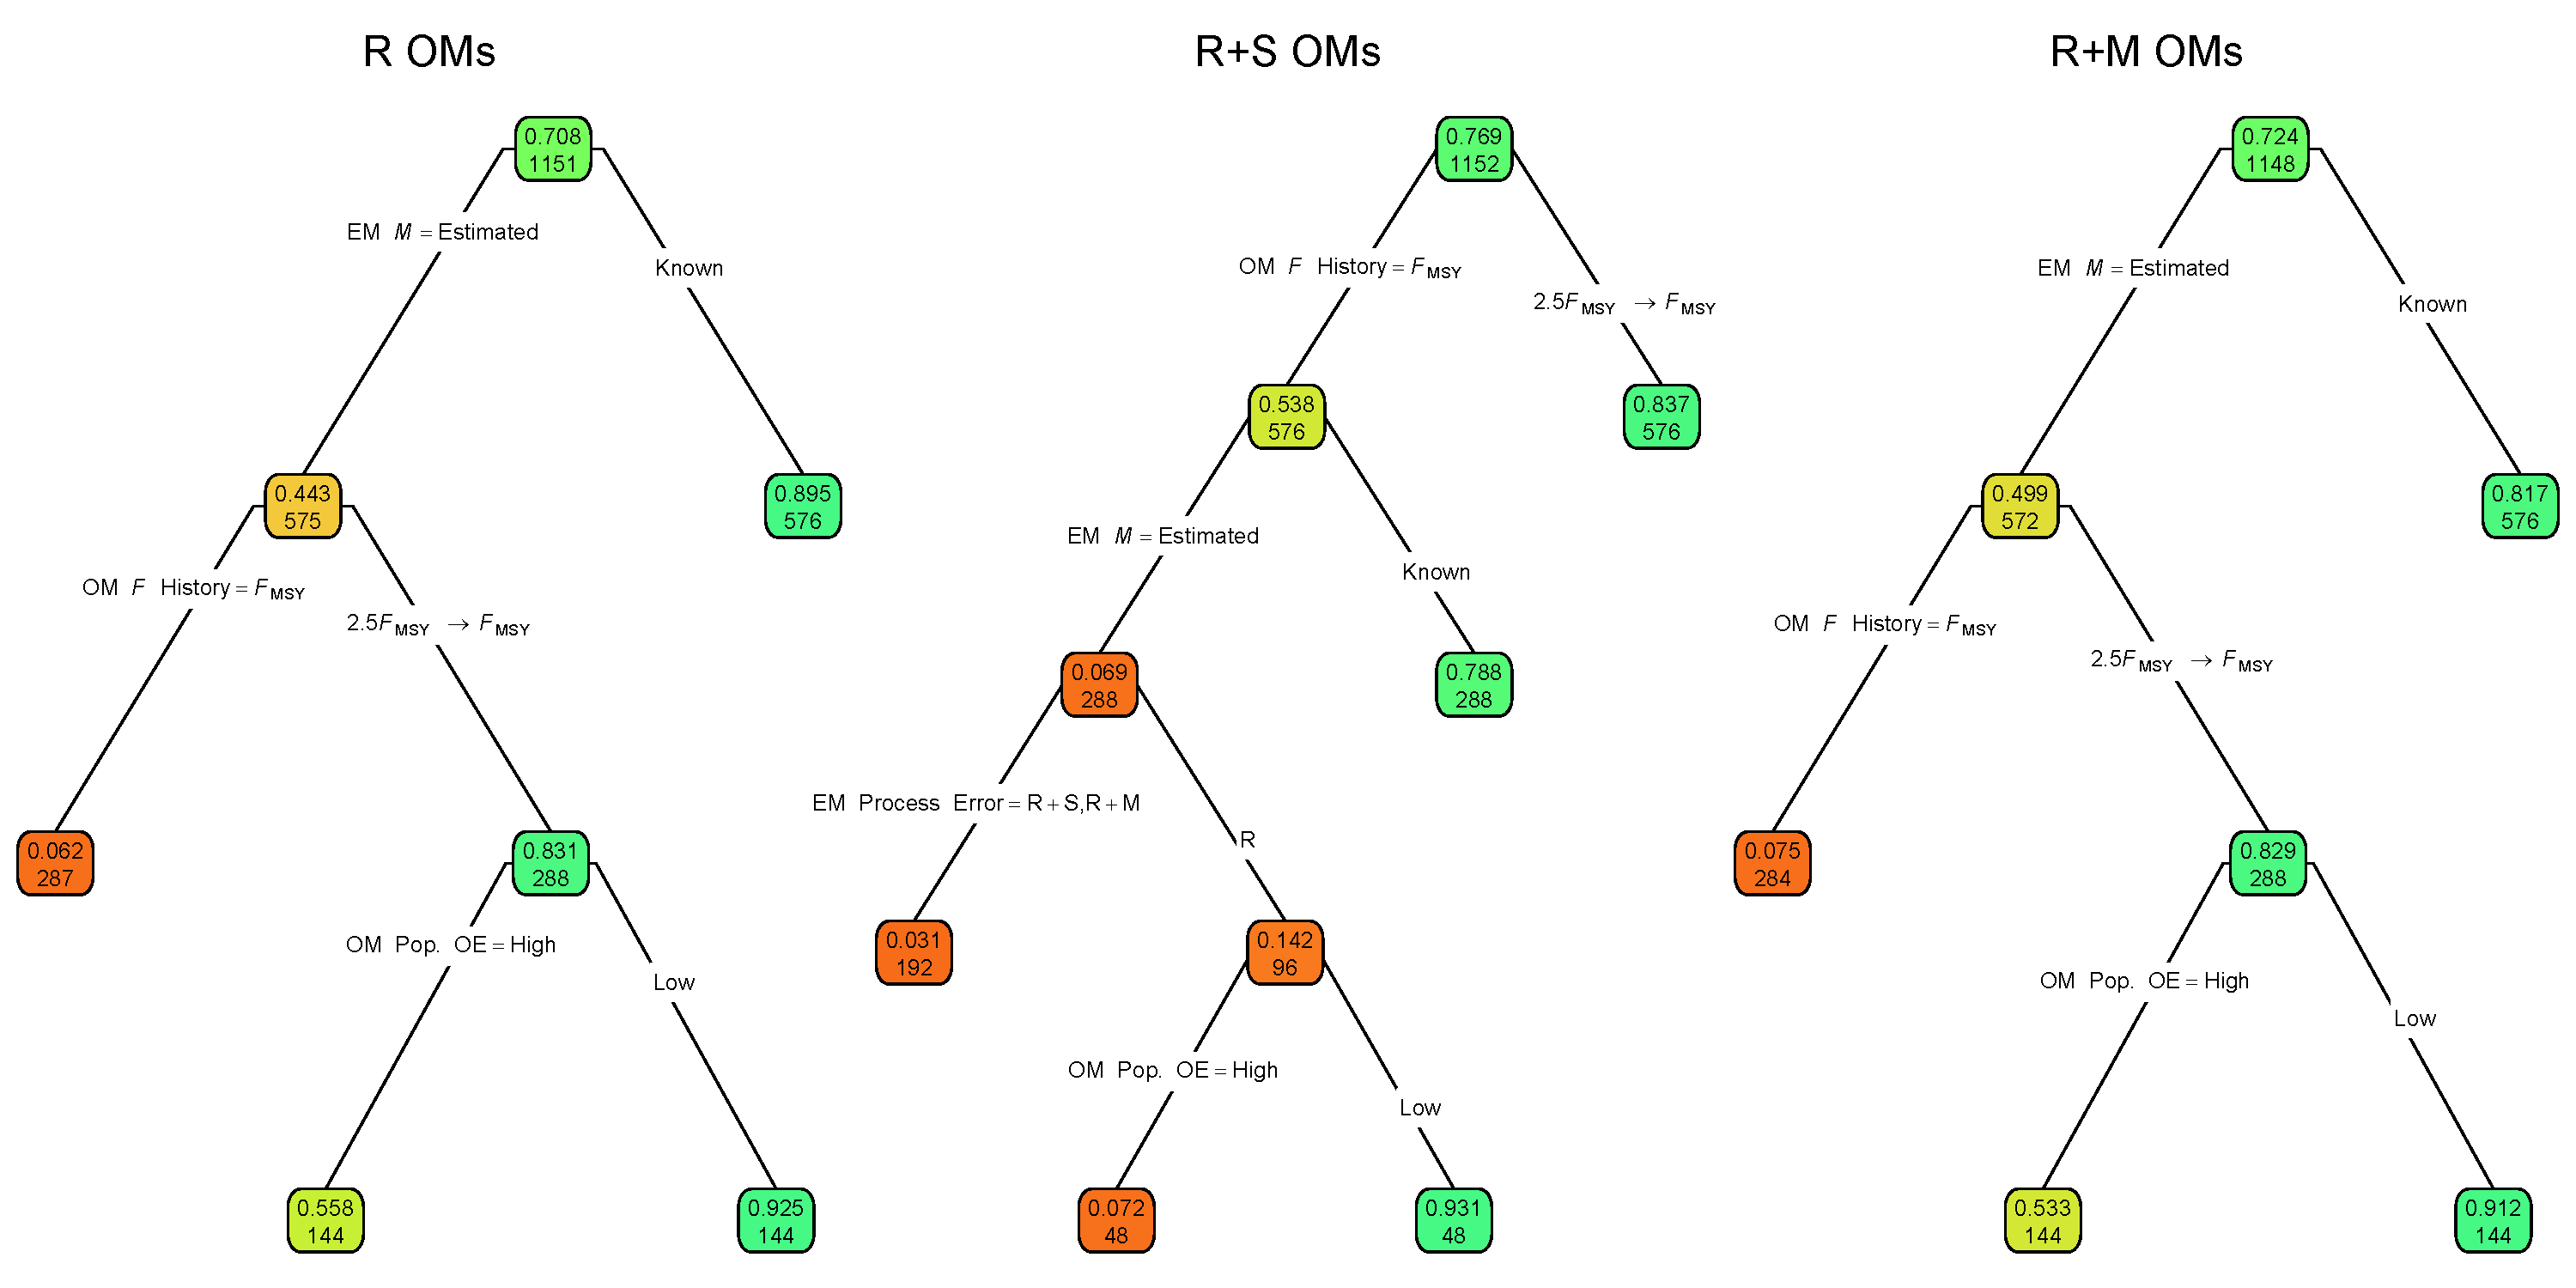
\includegraphics[width = 1.4\textwidth]{term_ssb_corr_regtree_plots}
%DIFDELCMD < \end{center}
%DIFDELCMD < %%%
%DIFDELCMD < \caption{%
{%DIFAUXCMD
\DIFdelFL{Regression trees indicating primary factors determining reductions in sums of squares for the correlation of terminal year SSB estimates and true values in EMs fitted to operating models (OMs) with process error on recruitment only (R), recruitment and apparent survival (R+S), or recruitment and natural mortality (R+M). Each node shows the median error (top) and number of observations (bottom) for the corresponding subset. Lower or higher median correlations are indicated by more red or green polygons, respectively.}}%DIFAUXCMD
%DIFDELCMD < \label{term_ssb_corr_regtree}
%DIFDELCMD < \end{figure}
%DIFDELCMD < \end{landscape}
%DIFDELCMD < \pagebreak
%DIFDELCMD < 

%DIFDELCMD < %%%
\DIFdelend \begin{table}
\caption{\DIFdelbeginFL \DIFdelFL{Operating (OM) and estimating model (EM) attributes used }\DIFdelendFL \DIFaddbeginFL \DIFaddFL{Percent reduction }\DIFaddendFL in \DIFdelbeginFL \DIFdelFL{analyses of }\DIFdelendFL deviance \DIFdelbeginFL \DIFdelFL{reduction and classification and }\DIFdelendFL \DIFaddbeginFL \DIFaddFL{for logistic }\DIFaddendFL regression \DIFdelbeginFL \DIFdelFL{trees. R, R+S, and R+M, denote }\DIFdelendFL models \DIFdelbeginFL \DIFdelFL{(OM or EM) with process error on recruitment only, recruitment and apparent survival, and recruitment and natural mortality, respectively}\DIFdelendFL \DIFaddbeginFL \DIFaddFL{fit to indicators of whether CIs for covariate effect estimates includes the true value}\DIFaddendFL . \DIFdelbeginFL \DIFdelFL{SD denotes standard deviation }\DIFdelendFL \DIFaddbeginFL \DIFaddFL{See Tables \ref{convergence_PRD_table} }\DIFaddendFL and \DIFdelbeginFL %DIFDELCMD < \Fmsy %%%
\DIFdelFL{is the fishing mortality rate that acheives maximum sustainable yield}\DIFdelendFL \DIFaddbeginFL \DIFaddFL{\ref{factor_table} for further details}\DIFaddendFL .}\DIFdelbeginFL %DIFDELCMD < \label{factor_table}
%DIFDELCMD < %%%
\DIFdelendFL \DIFaddbeginFL \label{ecov_beta_ci_coverage_PRD_table}
\DIFaddendFL {\begin{center}
\DIFdelbeginFL %DIFDELCMD < \begin{tabular}{lc}
%DIFDELCMD < \hline\hline
%DIFDELCMD < %%%
%DIFDELCMD < \multicolumn{1}{c}{%
{%DIFAUXCMD
\DIFdelFL{Factor}}%DIFAUXCMD
%DIFDELCMD < &%%%
%DIFDELCMD < \multicolumn{1}{c}{%
{%DIFAUXCMD
\DIFdelFL{Levels}}%DIFAUXCMD
%DIFDELCMD < \tabularnewline
%DIFDELCMD < \hline
%DIFDELCMD < %%%
\DIFdelFL{OM Process error}%DIFDELCMD < &%%%
\DIFdelFL{R, R+S, R+M}%DIFDELCMD < \tabularnewline
%DIFDELCMD < %%%
\DIFdelFL{OM Fishing History}%DIFDELCMD < &%%%
\DIFdelFL{$F_{\text{MSY}}$, $2.5F_{\text{MSY}} \rightarrow F_{\text{MSY}}$}%DIFDELCMD < \tabularnewline
%DIFDELCMD < %%%
\DIFdelFL{OM Covariate effect size ($\beta_E$)}%DIFDELCMD < &%%%
\DIFdelFL{0, 0.25, 0.5}%DIFDELCMD < \tabularnewline
%DIFDELCMD < %%%
\DIFdelFL{OM Population Observation Error}%DIFDELCMD < &%%%
\DIFdelFL{Low, High}%DIFDELCMD < \tabularnewline
%DIFDELCMD < %%%
\DIFdelFL{OM Covariate Observation Error}%DIFDELCMD < &%%%
\DIFdelFL{Low ($\sigma_e = 0.1$), High ($\sigma_e = 0.5$)}%DIFDELCMD < \tabularnewline
%DIFDELCMD < %%%
\DIFdelFL{OM Covariate Process Error SD ($\sigma_E$)}%DIFDELCMD < &%%%
\DIFdelFL{0.1, 0.5}%DIFDELCMD < \tabularnewline
%DIFDELCMD < %%%
\DIFdelFL{OM Covariate Process Error Correlation ($\rho_E$)}%DIFDELCMD < &%%%
\DIFdelFL{0, 0.5}%DIFDELCMD < \tabularnewline
%DIFDELCMD < %%%
\DIFdelFL{EM Process Error}%DIFDELCMD < &%%%
\DIFdelFL{R, R+S, R+M}%DIFDELCMD < \tabularnewline
%DIFDELCMD < %%%
\DIFdelFL{EM Covariate Effect}%DIFDELCMD < &%%%
\DIFdelFL{None ($\beta_E = 0$), $\beta_E$ estimated}%DIFDELCMD < \tabularnewline
%DIFDELCMD < %%%
\DIFdelFL{EM Median Natural Mortality Rate Parameter ($\beta_M$)}%DIFDELCMD < &%%%
\DIFdelFL{Known, Estimated}%DIFDELCMD < \tabularnewline
%DIFDELCMD < \hline
%DIFDELCMD < \end{tabular}\end{center}
%DIFDELCMD < }
%DIFDELCMD < \end{table}
%DIFDELCMD < \pagebreak
%DIFDELCMD < \clearpage
%DIFDELCMD < 

%DIFDELCMD < \begin{table}
%DIFDELCMD < %%%
%DIFDELCMD < \caption{%
{%DIFAUXCMD
\DIFdelFL{Percent reduction in deviance for linear regression models fit to errors in estimation of the Hessian-based standard error of the estimates of the covariate effect on $M$ ($\widehat {\text{SE}}\left(\widehat \beta_E\right)$). Table rows give each operating model (OM) and estimating model (EM) factor included individually, combined, and with second and third order interactions. Table columns are operating models (OMs) with process error on recruitment only (R), recruitment and apparent survival (R+S), or recruitment and natural mortality (R+M).}}%DIFAUXCMD
%DIFDELCMD < \label{bias_ecov_beta_se_PRD_table}
%DIFDELCMD < {\begin{center}
%DIFDELCMD < %%%
\DIFdelendFL \begin{tabular}{lrrr}
\hline\hline
\multicolumn{1}{l}{Factor}&\multicolumn{1}{c}{R}&\multicolumn{1}{c}{R+S}&\multicolumn{1}{c}{R+M}\tabularnewline
\hline
OM $F$ history& \DIFdelbeginFL \DIFdelFL{1.84}\DIFdelendFL \DIFaddbeginFL \DIFaddFL{0.24}\DIFaddendFL & \DIFdelbeginFL \DIFdelFL{2.68}\DIFdelendFL \DIFaddbeginFL \DIFaddFL{0.05}\DIFaddendFL & \DIFdelbeginFL \DIFdelFL{4.00}\DIFdelendFL \DIFaddbeginFL \DIFaddFL{0.01}\DIFaddendFL \tabularnewline
OM Obs. Error& \DIFdelbeginFL \DIFdelFL{0.06}\DIFdelendFL \DIFaddbeginFL \DIFaddFL{1.36}\DIFaddendFL & \DIFdelbeginFL \DIFdelFL{2.74}\DIFdelendFL \DIFaddbeginFL \DIFaddFL{1.91}\DIFaddendFL & \DIFdelbeginFL \DIFdelFL{8.04}\DIFdelendFL \DIFaddbeginFL \DIFaddFL{1.78}\DIFaddendFL \tabularnewline
OM $\sigma_e$& \DIFdelbeginFL \DIFdelFL{6.27}\DIFdelendFL \DIFaddbeginFL \DIFaddFL{8.26}\DIFaddendFL & \DIFdelbeginFL \DIFdelFL{7.28}\DIFdelendFL \DIFaddbeginFL \DIFaddFL{0.24}\DIFaddendFL & \DIFdelbeginFL \DIFdelFL{12.83}\DIFdelendFL \DIFaddbeginFL \DIFaddFL{0.92}\DIFaddendFL \tabularnewline
OM $\sigma_E$& \DIFdelbeginFL \DIFdelFL{0.48}\DIFdelendFL \DIFaddbeginFL \DIFaddFL{0.92}\DIFaddendFL & \DIFdelbeginFL \DIFdelFL{1.05}\DIFdelendFL \DIFaddbeginFL \DIFaddFL{1.70}\DIFaddendFL & \DIFdelbeginFL \DIFdelFL{0.46}\DIFdelendFL \DIFaddbeginFL \DIFaddFL{1.56}\DIFaddendFL \tabularnewline
OM $\rho_{E}$& \DIFdelbeginFL \DIFdelFL{0.17}\DIFdelendFL \DIFaddbeginFL \DIFaddFL{0.03}\DIFaddendFL & \DIFdelbeginFL \DIFdelFL{0.01}\DIFdelendFL \DIFaddbeginFL \DIFaddFL{0.05}\DIFaddendFL & \DIFdelbeginFL \DIFdelFL{0.02}\DIFdelendFL \DIFaddbeginFL \DIFaddFL{0.06}\DIFaddendFL \tabularnewline
OM $\beta_{E}$&\DIFdelbeginFL \DIFdelFL{0.37}\DIFdelendFL \DIFaddbeginFL \DIFaddFL{11.10}\DIFaddendFL & \DIFdelbeginFL \DIFdelFL{0.01}\DIFdelendFL \DIFaddbeginFL \DIFaddFL{0.68}\DIFaddendFL & \DIFdelbeginFL \DIFdelFL{0.05}\DIFdelendFL \DIFaddbeginFL \DIFaddFL{2.72}\DIFaddendFL \tabularnewline
EM Process Error& \DIFdelbeginFL \DIFdelFL{2.90}\DIFdelendFL \DIFaddbeginFL \DIFaddFL{0.01}\DIFaddendFL & \DIFdelbeginFL \DIFdelFL{3.89}\DIFdelendFL \DIFaddbeginFL \DIFaddFL{6.51}\DIFaddendFL & \DIFdelbeginFL \DIFdelFL{2.98}\DIFdelendFL \DIFaddbeginFL \DIFaddFL{0.27}\DIFaddendFL \tabularnewline
EM $M$ assumption& \DIFdelbeginFL \DIFdelFL{0.15}\DIFdelendFL \DIFaddbeginFL \DIFaddFL{0.25}\DIFaddendFL & \DIFdelbeginFL \DIFdelFL{0.34}\DIFdelendFL \DIFaddbeginFL \DIFaddFL{0.29}\DIFaddendFL & \DIFdelbeginFL \DIFdelFL{0.47}\DIFdelendFL \DIFaddbeginFL \DIFaddFL{0.06}\DIFaddendFL \tabularnewline
All factors&\DIFdelbeginFL \DIFdelFL{13.01}\DIFdelendFL \DIFaddbeginFL \DIFaddFL{23.61}\DIFaddendFL &\DIFdelbeginFL \DIFdelFL{20.95}\DIFdelendFL \DIFaddbeginFL \DIFaddFL{12.16}\DIFaddendFL & \DIFdelbeginFL \DIFdelFL{29.24}\DIFdelendFL \DIFaddbeginFL \DIFaddFL{7.78}\DIFaddendFL \tabularnewline
+ All Two Way&\DIFdelbeginFL \DIFdelFL{28.58}\DIFdelendFL \DIFaddbeginFL \DIFaddFL{30.17}\DIFaddendFL &\DIFdelbeginFL \DIFdelFL{32.25}\DIFdelendFL \DIFaddbeginFL \DIFaddFL{18.08}\DIFaddendFL &\DIFdelbeginFL \DIFdelFL{42.77}\DIFdelendFL \DIFaddbeginFL \DIFaddFL{12.63}\DIFaddendFL \tabularnewline
+ All Three Way&\DIFdelbeginFL \DIFdelFL{44.44}\DIFdelendFL \DIFaddbeginFL \DIFaddFL{32.58}\DIFaddendFL &\DIFdelbeginFL \DIFdelFL{42.83}\DIFdelendFL \DIFaddbeginFL \DIFaddFL{20.62}\DIFaddendFL &\DIFdelbeginFL \DIFdelFL{51.84}\DIFdelendFL \DIFaddbeginFL \DIFaddFL{14.87}\DIFaddendFL \tabularnewline
\hline
\end{tabular}\end{center}
}
\end{table}
\pagebreak

\begin{table}
\caption{Percent reduction in deviance for linear regression models fit to errors in \DIFdelbeginFL \DIFdelFL{estimation of the Hessian-based standard error of the estimates of the median $M$ parameter }\DIFdelendFL \DIFaddbeginFL \DIFaddFL{terminal year natural mortality rate }\DIFaddendFL (\DIFdelbeginFL \DIFdelFL{$\widehat {\text{SE}}\left(\widehat \beta_M\right)$}\DIFdelendFL \DIFaddbeginFL \DIFaddFL{$M$}\DIFaddendFL ) \DIFaddbeginFL \DIFaddFL{as measured by Eq}\DIFaddendFL . \DIFdelbeginFL \DIFdelFL{Table rows give each operating model (OM) and estimating model (EM) factor included individually, combined, and with second and third order interactions}\DIFdelendFL \DIFaddbeginFL \DIFaddFL{\ref{relerror_trans_response}}\DIFaddendFL . \DIFdelbeginFL \DIFdelFL{Table columns are operating models (OMs) with process error on recruitment only (R), recruitment }\DIFdelendFL \DIFaddbeginFL \DIFaddFL{See Tables \ref{convergence_PRD_table} }\DIFaddendFL and \DIFdelbeginFL \DIFdelFL{apparent survival (R+S), or recruitment and natural mortality (R+M)}\DIFdelendFL \DIFaddbeginFL \DIFaddFL{\ref{factor_table} for further details}\DIFaddendFL .}\DIFdelbeginFL %DIFDELCMD < \label{median_M_se_bias_PRD_table}
%DIFDELCMD < %%%
\DIFdelendFL \DIFaddbeginFL \label{bias_M_PRD_table}
\DIFaddendFL {\begin{center}
\begin{tabular}{lrrr}
\hline\hline
\multicolumn{1}{l}{Factor}&\multicolumn{1}{c}{R}&\multicolumn{1}{c}{R+S}&\multicolumn{1}{c}{R+M}\tabularnewline
\hline
\DIFaddbeginFL \DIFaddFL{Convergence}&\DIFaddFL{\textless  0.01}& \DIFaddFL{0.18}& \DIFaddFL{0.01}\tabularnewline
\DIFaddendFL OM $F$ history& \DIFdelbeginFL \DIFdelFL{0.55}\DIFdelendFL \DIFaddbeginFL \DIFaddFL{0.66}\DIFaddendFL & \DIFdelbeginFL \DIFdelFL{12.91}\DIFdelendFL \DIFaddbeginFL \DIFaddFL{2.69}\DIFaddendFL & \DIFdelbeginFL \DIFdelFL{3.65}\DIFdelendFL \DIFaddbeginFL \DIFaddFL{1.00}\DIFaddendFL \tabularnewline
OM Obs. Error& \DIFdelbeginFL \DIFdelFL{0.98}\DIFdelendFL \DIFaddbeginFL \DIFaddFL{0.29}\DIFaddendFL & \DIFdelbeginFL \DIFdelFL{0.01}\DIFdelendFL \DIFaddbeginFL \DIFaddFL{0.43}\DIFaddendFL & \DIFdelbeginFL \DIFdelFL{0.07}\DIFdelendFL \DIFaddbeginFL \DIFaddFL{0.16}\DIFaddendFL \tabularnewline
OM $\sigma_e$&\textless  0.01&\DIFdelbeginFL \DIFdelFL{0.03}\DIFdelendFL \DIFaddbeginFL \DIFaddFL{\textless  0.01}\DIFaddendFL &\DIFdelbeginFL \DIFdelFL{0.11}\DIFdelendFL \DIFaddbeginFL \DIFaddFL{\textless  0.01}\DIFaddendFL \tabularnewline
OM $\sigma_E$& \DIFdelbeginFL \DIFdelFL{0.13}\DIFdelendFL \DIFaddbeginFL \DIFaddFL{0.02}\DIFaddendFL &\DIFdelbeginFL \DIFdelFL{0.03}\DIFdelendFL \DIFaddbeginFL \DIFaddFL{\textless  0.01}\DIFaddendFL &\DIFdelbeginFL \DIFdelFL{0.19}\DIFdelendFL \DIFaddbeginFL \DIFaddFL{\textless  0.01}\DIFaddendFL \tabularnewline
OM $\rho_{E}$&\textless  0.01& \DIFdelbeginFL \DIFdelFL{0.02}\DIFdelendFL \DIFaddbeginFL \DIFaddFL{0.01}\DIFaddendFL &\textless  0.01\tabularnewline
OM $\beta_{E}$& \DIFdelbeginFL \DIFdelFL{0.12}\DIFdelendFL \DIFaddbeginFL \DIFaddFL{0.03}\DIFaddendFL & \DIFdelbeginFL \DIFdelFL{0.07}\DIFdelendFL \DIFaddbeginFL \DIFaddFL{0.01}\DIFaddendFL & \DIFdelbeginFL \DIFdelFL{0.23}\DIFdelendFL \DIFaddbeginFL \DIFaddFL{0.01}\DIFaddendFL \tabularnewline
EM Process Error& \DIFdelbeginFL \DIFdelFL{3.16}\DIFdelendFL \DIFaddbeginFL \DIFaddFL{0.22}\DIFaddendFL & \DIFdelbeginFL \DIFdelFL{8.79}\DIFdelendFL \DIFaddbeginFL \DIFaddFL{1.42}\DIFaddendFL & \DIFdelbeginFL \DIFdelFL{6.83}\DIFdelendFL \DIFaddbeginFL \DIFaddFL{0.43}\DIFaddendFL \tabularnewline
EM $\beta_{E}$ assumption& \DIFdelbeginFL \DIFdelFL{0.18}\DIFdelendFL \DIFaddbeginFL \DIFaddFL{0.35}\DIFaddendFL & \DIFdelbeginFL \DIFdelFL{8.96}\DIFdelendFL \DIFaddbeginFL \DIFaddFL{1.07}\DIFaddendFL & \DIFdelbeginFL \DIFdelFL{3.81}\DIFdelendFL \DIFaddbeginFL \DIFaddFL{0.39}\DIFaddendFL \tabularnewline
\DIFaddbeginFL \DIFaddFL{EM $M$ assumption}& \DIFaddFL{0.84}& \DIFaddFL{5.10}& \DIFaddFL{1.22}\tabularnewline
\DIFaddendFL All factors& \DIFdelbeginFL \DIFdelFL{5.32}\DIFdelendFL \DIFaddbeginFL \DIFaddFL{2.56}\DIFaddendFL &\DIFdelbeginFL \DIFdelFL{28.39}\DIFdelendFL \DIFaddbeginFL \DIFaddFL{10.83}\DIFaddendFL & \DIFdelbeginFL \DIFdelFL{14.71}\DIFdelendFL \DIFaddbeginFL \DIFaddFL{3.37}\DIFaddendFL \tabularnewline
+ All Two Way& \DIFdelbeginFL \DIFdelFL{11.80}\DIFdelendFL \DIFaddbeginFL \DIFaddFL{5.41}\DIFaddendFL &\DIFdelbeginFL \DIFdelFL{44.67}\DIFdelendFL \DIFaddbeginFL \DIFaddFL{18.75}\DIFaddendFL & \DIFdelbeginFL \DIFdelFL{22.70}\DIFdelendFL \DIFaddbeginFL \DIFaddFL{6.38}\DIFaddendFL \tabularnewline
+ All Three Way& \DIFdelbeginFL \DIFdelFL{17.83}\DIFdelendFL \DIFaddbeginFL \DIFaddFL{7.93}\DIFaddendFL &\DIFdelbeginFL \DIFdelFL{51.54}\DIFdelendFL \DIFaddbeginFL \DIFaddFL{22.49}\DIFaddendFL & \DIFdelbeginFL \DIFdelFL{29.46}\DIFdelendFL \DIFaddbeginFL \DIFaddFL{8.76}\DIFaddendFL \tabularnewline
\hline
\end{tabular}\end{center}
}
\end{table}
\pagebreak

\begin{table}
\caption{Percent reduction in deviance for linear regression models fit to log-transformed RMSE of terminal year natural mortality ($M$). \DIFdelbeginFL \DIFdelFL{Table rows give each operating model (OM) }\DIFdelendFL \DIFaddbeginFL \DIFaddFL{See Tables \ref{convergence_PRD_table} }\DIFaddendFL and \DIFdelbeginFL \DIFdelFL{estimating model (EM) factor included individually, combined, and with second and third order interactions}\DIFdelendFL \DIFaddbeginFL \DIFaddFL{\ref{factor_table} for further details}\DIFaddendFL .\DIFdelbeginFL \DIFdelFL{Table columns are operating models (OMs) with process error on recruitment only (R), recruitment and apparent survival (R+S), or recruitment and natural mortality (R+M).}\DIFdelendFL }\label{rmse_M_PRD_table}
{\begin{center}
\begin{tabular}{lrrr}
\hline\hline
\multicolumn{1}{l}{Factor}&\multicolumn{1}{c}{R}&\multicolumn{1}{c}{R+S}&\multicolumn{1}{c}{R+M}\tabularnewline
\hline
OM $F$ history& 0.26& 2.21&14.65\tabularnewline
OM Obs. Error& 1.65& 0.71& 4.68\tabularnewline
OM $\sigma_e$& 0.02& 0.16& 0.01\tabularnewline
OM $\sigma_E$& 1.06& 1.23& 0.84\tabularnewline
OM $\rho_{E}$& 0.02& 0.01&\textless  0.01\tabularnewline
OM $\beta_{E}$& 3.73& 1.94& 1.14\tabularnewline
EM Process Error& 2.04& 3.85& 0.87\tabularnewline
$EM \beta_{E}$ assumption& 0.19& 0.59& 0.07\tabularnewline
EM $M$ assumption&22.28&45.15&44.70\tabularnewline
All factors&32.83&56.71&66.99\tabularnewline
+ All Two Way&57.65&84.17&87.96\tabularnewline
+ All Three Way&74.93&94.57&91.94\tabularnewline
\hline
\end{tabular}\end{center}
}
\end{table}
\pagebreak

\begin{table}
\caption{Percent reduction in deviance for linear regression models fit to correlation of terminal year natural mortality ($M$) estimates and true values. \DIFdelbeginFL \DIFdelFL{Table rows give each operating model (OM) }\DIFdelendFL \DIFaddbeginFL \DIFaddFL{See Tables \ref{convergence_PRD_table} }\DIFaddendFL and \DIFdelbeginFL \DIFdelFL{estimating model (EM) factor included individually, combined, and with second and third order interactions}\DIFdelendFL \DIFaddbeginFL \DIFaddFL{\ref{factor_table} for further details}\DIFaddendFL .\DIFdelbeginFL \DIFdelFL{Table columns are operating models (OMs) with process error on recruitment only (R), recruitment and apparent survival (R+S), or recruitment and natural mortality (R+M).}\DIFdelendFL }\label{corr_M_PRD_table}
{\begin{center}
\begin{tabular}{lrrr}
\hline\hline
\multicolumn{1}{l}{Factor}&\multicolumn{1}{c}{R}&\multicolumn{1}{c}{R+S}&\multicolumn{1}{c}{R+M}\tabularnewline
\hline
OM $F$ history& 0.05& 0.02& 0.37\tabularnewline
OM Obs. Error& 2.00& 0.89& 3.73\tabularnewline
OM $\sigma_e$& 2.30& 2.56& 0.37\tabularnewline
OM $\sigma_E$&14.91&13.78& 3.03\tabularnewline
OM $\rho_{E}$& 1.98& 0.33& 0.14\tabularnewline
OM $\beta_{E}$& 0.41& 3.76& 3.87\tabularnewline
EM Process Error& 0.43& 1.52& 0.62\tabularnewline
$EM \beta_{E}$ assumption&12.72&12.30& 1.56\tabularnewline
EM $M$ assumption&12.34& 7.16& 3.03\tabularnewline
All factors&42.11&38.31&15.76\tabularnewline
+ All Two Way&63.38&62.40&31.99\tabularnewline
+ All Three Way&72.79&75.98&46.62\tabularnewline
\hline
\end{tabular}\end{center}
}
\end{table}
\pagebreak

\begin{table}
\caption{Percent reduction in deviance for linear regression models fit to \DIFdelbeginFL \DIFdelFL{log-transformed RMSE of }\DIFdelendFL \DIFaddbeginFL \DIFaddFL{errors in }\DIFaddendFL terminal year spawning stock biomass (SSB) \DIFaddbeginFL \DIFaddFL{as measured by Eq}\DIFaddendFL . \DIFdelbeginFL \DIFdelFL{Table rows give each operating model (OM) and estimating model (EM) factor included individually, combined, and with second and third order interactions}\DIFdelendFL \DIFaddbeginFL \DIFaddFL{\ref{relerror_trans_response}}\DIFaddendFL . \DIFdelbeginFL \DIFdelFL{Table columns are operating models (OMs) with process error on recruitment only (R), recruitment }\DIFdelendFL \DIFaddbeginFL \DIFaddFL{See Tables \ref{convergence_PRD_table} }\DIFaddendFL and \DIFdelbeginFL \DIFdelFL{apparent survival (R+S), or recruitment and natural mortality (R+M)}\DIFdelendFL \DIFaddbeginFL \DIFaddFL{\ref{factor_table} for further details}\DIFaddendFL .}\DIFdelbeginFL %DIFDELCMD < \label{rmse_SSB_PRD_table}
%DIFDELCMD < %%%
\DIFdelendFL \DIFaddbeginFL \label{bias_SSB_PRD_table}
\DIFaddendFL {\begin{center}
\begin{tabular}{lrrr}
\hline\hline
\multicolumn{1}{l}{Factor}&\multicolumn{1}{c}{R}&\multicolumn{1}{c}{R+S}&\multicolumn{1}{c}{R+M}\tabularnewline
\hline
\DIFdelbeginFL \DIFdelFL{OM $F$ history}\DIFdelendFL \DIFaddbeginFL \DIFaddFL{Convergence}\DIFaddendFL & \DIFdelbeginFL \DIFdelFL{19.88}%DIFDELCMD < &%%%
\DIFdelFL{32.67}%DIFDELCMD < &%%%
\DIFdelFL{20.92}%DIFDELCMD < \tabularnewline
%DIFDELCMD < %%%
\DIFdelFL{OM Obs. Error}%DIFDELCMD < & %%%
\DIFdelFL{2.21}%DIFDELCMD < & %%%
\DIFdelFL{0.11}%DIFDELCMD < & %%%
\DIFdelFL{1.48}%DIFDELCMD < \tabularnewline
%DIFDELCMD < %%%
\DIFdelFL{OM $\sigma_e$}%DIFDELCMD < & %%%
\DIFdelFL{0.05}%DIFDELCMD < & %%%
\DIFdelFL{0.16}%DIFDELCMD < & %%%
\DIFdelFL{0.03}%DIFDELCMD < \tabularnewline
%DIFDELCMD < %%%
\DIFdelFL{OM $\sigma_E$}%DIFDELCMD < & %%%
\DIFdelFL{0.08}%DIFDELCMD < & %%%
\DIFdelFL{0.16}%DIFDELCMD < & %%%
\DIFdelendFL 0.02\DIFdelbeginFL %DIFDELCMD < \tabularnewline
%DIFDELCMD < %%%
\DIFdelFL{OM $\rho_{E}$}\DIFdelendFL & \DIFdelbeginFL \DIFdelFL{0.03}%DIFDELCMD < &%%%
\DIFdelFL{\textless  0.01}%DIFDELCMD < & %%%
\DIFdelFL{0.02}%DIFDELCMD < \tabularnewline
%DIFDELCMD < %%%
\DIFdelFL{OM $\beta_{E}$}%DIFDELCMD < & %%%
\DIFdelFL{0.05}%DIFDELCMD < & %%%
\DIFdelFL{0.03}%DIFDELCMD < & %%%
\DIFdelFL{0.14}%DIFDELCMD < \tabularnewline
%DIFDELCMD < %%%
\DIFdelFL{EM Process Error}%DIFDELCMD < & %%%
\DIFdelFL{5.72}%DIFDELCMD < & %%%
\DIFdelendFL 0.13&\DIFdelbeginFL \DIFdelFL{5.73}%DIFDELCMD < \tabularnewline
%DIFDELCMD < %%%
\DIFdelFL{$EM \beta_{E}$ assumption}%DIFDELCMD < & %%%
\DIFdelFL{0.03}%DIFDELCMD < & %%%
\DIFdelFL{0.79}%DIFDELCMD < & %%%
\DIFdelFL{0.05}%DIFDELCMD < \tabularnewline
%DIFDELCMD < %%%
\DIFdelFL{EM $M$ assumption}%DIFDELCMD < &%%%
\DIFdelFL{20.05}%DIFDELCMD < &%%%
\DIFdelFL{21.11}%DIFDELCMD < &%%%
\DIFdelFL{19.43}%DIFDELCMD < \tabularnewline
%DIFDELCMD < %%%
\DIFdelFL{All factors}%DIFDELCMD < &%%%
\DIFdelFL{48.09}%DIFDELCMD < &%%%
\DIFdelFL{55.17}%DIFDELCMD < &%%%
\DIFdelFL{47.82}%DIFDELCMD < \tabularnewline
%DIFDELCMD < %%%
\DIFdelFL{+ All Two Way}%DIFDELCMD < &%%%
\DIFdelFL{79.09}%DIFDELCMD < &%%%
\DIFdelFL{80.98}%DIFDELCMD < &%%%
\DIFdelFL{78.40}%DIFDELCMD < \tabularnewline
%DIFDELCMD < %%%
\DIFdelFL{+ All Three Way}%DIFDELCMD < &%%%
\DIFdelFL{88.30}%DIFDELCMD < &%%%
\DIFdelFL{89.49}%DIFDELCMD < &%%%
\DIFdelFL{87.67}%DIFDELCMD < \tabularnewline
%DIFDELCMD < \hline
%DIFDELCMD < \end{tabular}\end{center}
%DIFDELCMD < }
%DIFDELCMD < \end{table}
%DIFDELCMD < \pagebreak
%DIFDELCMD < 

%DIFDELCMD < \begin{table}
%DIFDELCMD < %%%
%DIFDELCMD < \caption{%
{%DIFAUXCMD
\DIFdelFL{Percent reduction in deviance for linear regression models fit to correlation of terminal year spawning stock biomass (SSB) estimates and true values. Table rows give each operating model (OM) and estimating model (EM) factor included individually, combined, and with second and third order interactions. Table columns are operating models (OMs) with process error on recruitment only (R), recruitment and apparent survival (R+S), or recruitment and natural mortality (R+M).}}%DIFAUXCMD
%DIFDELCMD < \label{corr_ssb_PRD_table}
%DIFDELCMD < {\begin{center}
%DIFDELCMD < \begin{tabular}{lrrr}
%DIFDELCMD < \hline\hline
%DIFDELCMD < %%%
%DIFDELCMD < \multicolumn{1}{l}{%
{%DIFAUXCMD
\DIFdelFL{Factor}}%DIFAUXCMD
%DIFDELCMD < &%%%
%DIFDELCMD < \multicolumn{1}{c}{%
{%DIFAUXCMD
\DIFdelFL{R}}%DIFAUXCMD
%DIFDELCMD < &%%%
%DIFDELCMD < \multicolumn{1}{c}{%
{%DIFAUXCMD
\DIFdelFL{R+S}}%DIFAUXCMD
%DIFDELCMD < &%%%
%DIFDELCMD < \multicolumn{1}{c}{%
{%DIFAUXCMD
\DIFdelFL{R+M}}%DIFAUXCMD
%DIFDELCMD < \tabularnewline
%DIFDELCMD < \hline
%DIFDELCMD < %%%
\DIFdelFL{OM $F$ history}%DIFDELCMD < &%%%
\DIFdelFL{19.27}%DIFDELCMD < &%%%
\DIFdelFL{25.70}%DIFDELCMD < &%%%
\DIFdelFL{19.59}%DIFDELCMD < \tabularnewline
%DIFDELCMD < %%%
\DIFdelFL{OM Obs. Error}%DIFDELCMD < &%%%
\DIFdelFL{12.53}%DIFDELCMD < & %%%
\DIFdelFL{3.60}%DIFDELCMD < & %%%
\DIFdelFL{9.46}%DIFDELCMD < \tabularnewline
%DIFDELCMD < %%%
\DIFdelFL{OM $\sigma_e$}%DIFDELCMD < & %%%
\DIFdelFL{0.08}%DIFDELCMD < & %%%
\DIFdelFL{0.44}%DIFDELCMD < & %%%
\DIFdelFL{0.09}%DIFDELCMD < \tabularnewline
%DIFDELCMD < %%%
\DIFdelFL{OM $\sigma_E$}%DIFDELCMD < & %%%
\DIFdelFL{0.10}%DIFDELCMD < & %%%
\DIFdelFL{0.44}%DIFDELCMD < & %%%
\DIFdelFL{0.11}%DIFDELCMD < \tabularnewline
%DIFDELCMD < %%%
\DIFdelFL{OM $\rho_{E}$}%DIFDELCMD < &%%%
\DIFdelendFL \textless  0.01\DIFdelbeginFL %DIFDELCMD < &%%%
\DIFdelFL{\textless  0.01}%DIFDELCMD < & %%%
\DIFdelFL{0.09}\DIFdelendFL \tabularnewline
OM \DIFdelbeginFL \DIFdelFL{$\beta_{E}$}%DIFDELCMD < & %%%
\DIFdelFL{0.09}%DIFDELCMD < & %%%
\DIFdelFL{0.05}%DIFDELCMD < &%%%
\DIFdelFL{\textless  0.01}%DIFDELCMD < \tabularnewline
%DIFDELCMD < %%%
\DIFdelFL{EM Process Error}%DIFDELCMD < & %%%
\DIFdelFL{0.07}%DIFDELCMD < & %%%
\DIFdelFL{0.92}%DIFDELCMD < & %%%
\DIFdelFL{0.71}%DIFDELCMD < \tabularnewline
%DIFDELCMD < %%%
\DIFdelFL{$EM \beta_{E}$ assumption}%DIFDELCMD < &%%%
\DIFdelFL{\textless  0.01}%DIFDELCMD < & %%%
\DIFdelFL{1.32}%DIFDELCMD < & %%%
\DIFdelFL{0.38}%DIFDELCMD < \tabularnewline
%DIFDELCMD < %%%
\DIFdelFL{EM $M$ assumption}%DIFDELCMD < &%%%
\DIFdelFL{28.94}%DIFDELCMD < &%%%
\DIFdelFL{19.74}%DIFDELCMD < &%%%
\DIFdelFL{25.36}%DIFDELCMD < \tabularnewline
%DIFDELCMD < %%%
\DIFdelFL{All factors}%DIFDELCMD < &%%%
\DIFdelFL{61.19}%DIFDELCMD < &%%%
\DIFdelFL{52.21}%DIFDELCMD < &%%%
\DIFdelFL{56.09}%DIFDELCMD < \tabularnewline
%DIFDELCMD < %%%
\DIFdelFL{+ All Two Way}%DIFDELCMD < &%%%
\DIFdelFL{81.48}%DIFDELCMD < &%%%
\DIFdelFL{72.16}%DIFDELCMD < &%%%
\DIFdelFL{74.98}%DIFDELCMD < \tabularnewline
%DIFDELCMD < %%%
\DIFdelFL{+ All Three Way}%DIFDELCMD < &%%%
\DIFdelFL{85.23}%DIFDELCMD < &%%%
\DIFdelFL{83.22}%DIFDELCMD < &%%%
\DIFdelFL{80.48}%DIFDELCMD < \tabularnewline
%DIFDELCMD < \hline
%DIFDELCMD < \end{tabular}\end{center}
%DIFDELCMD < }
%DIFDELCMD < \end{table}
%DIFDELCMD < \pagebreak
%DIFDELCMD < 

%DIFDELCMD < \clearpage
%DIFDELCMD < 

%DIFDELCMD < %%%
\subsection*{\DIFdel{Convergence results}}%DIFAUXCMD
%DIFDELCMD < \label{convergence-results}
%DIFDELCMD < %%%
\addcontentsline{toc}{subsection}{\DIFdel{Convergence results}}
%DIFAUXCMD
%DIFDELCMD < 

%DIFDELCMD < \begin{landscape}
%DIFDELCMD < \begin{figure}
%DIFDELCMD < \begin{center}
%DIFDELCMD < 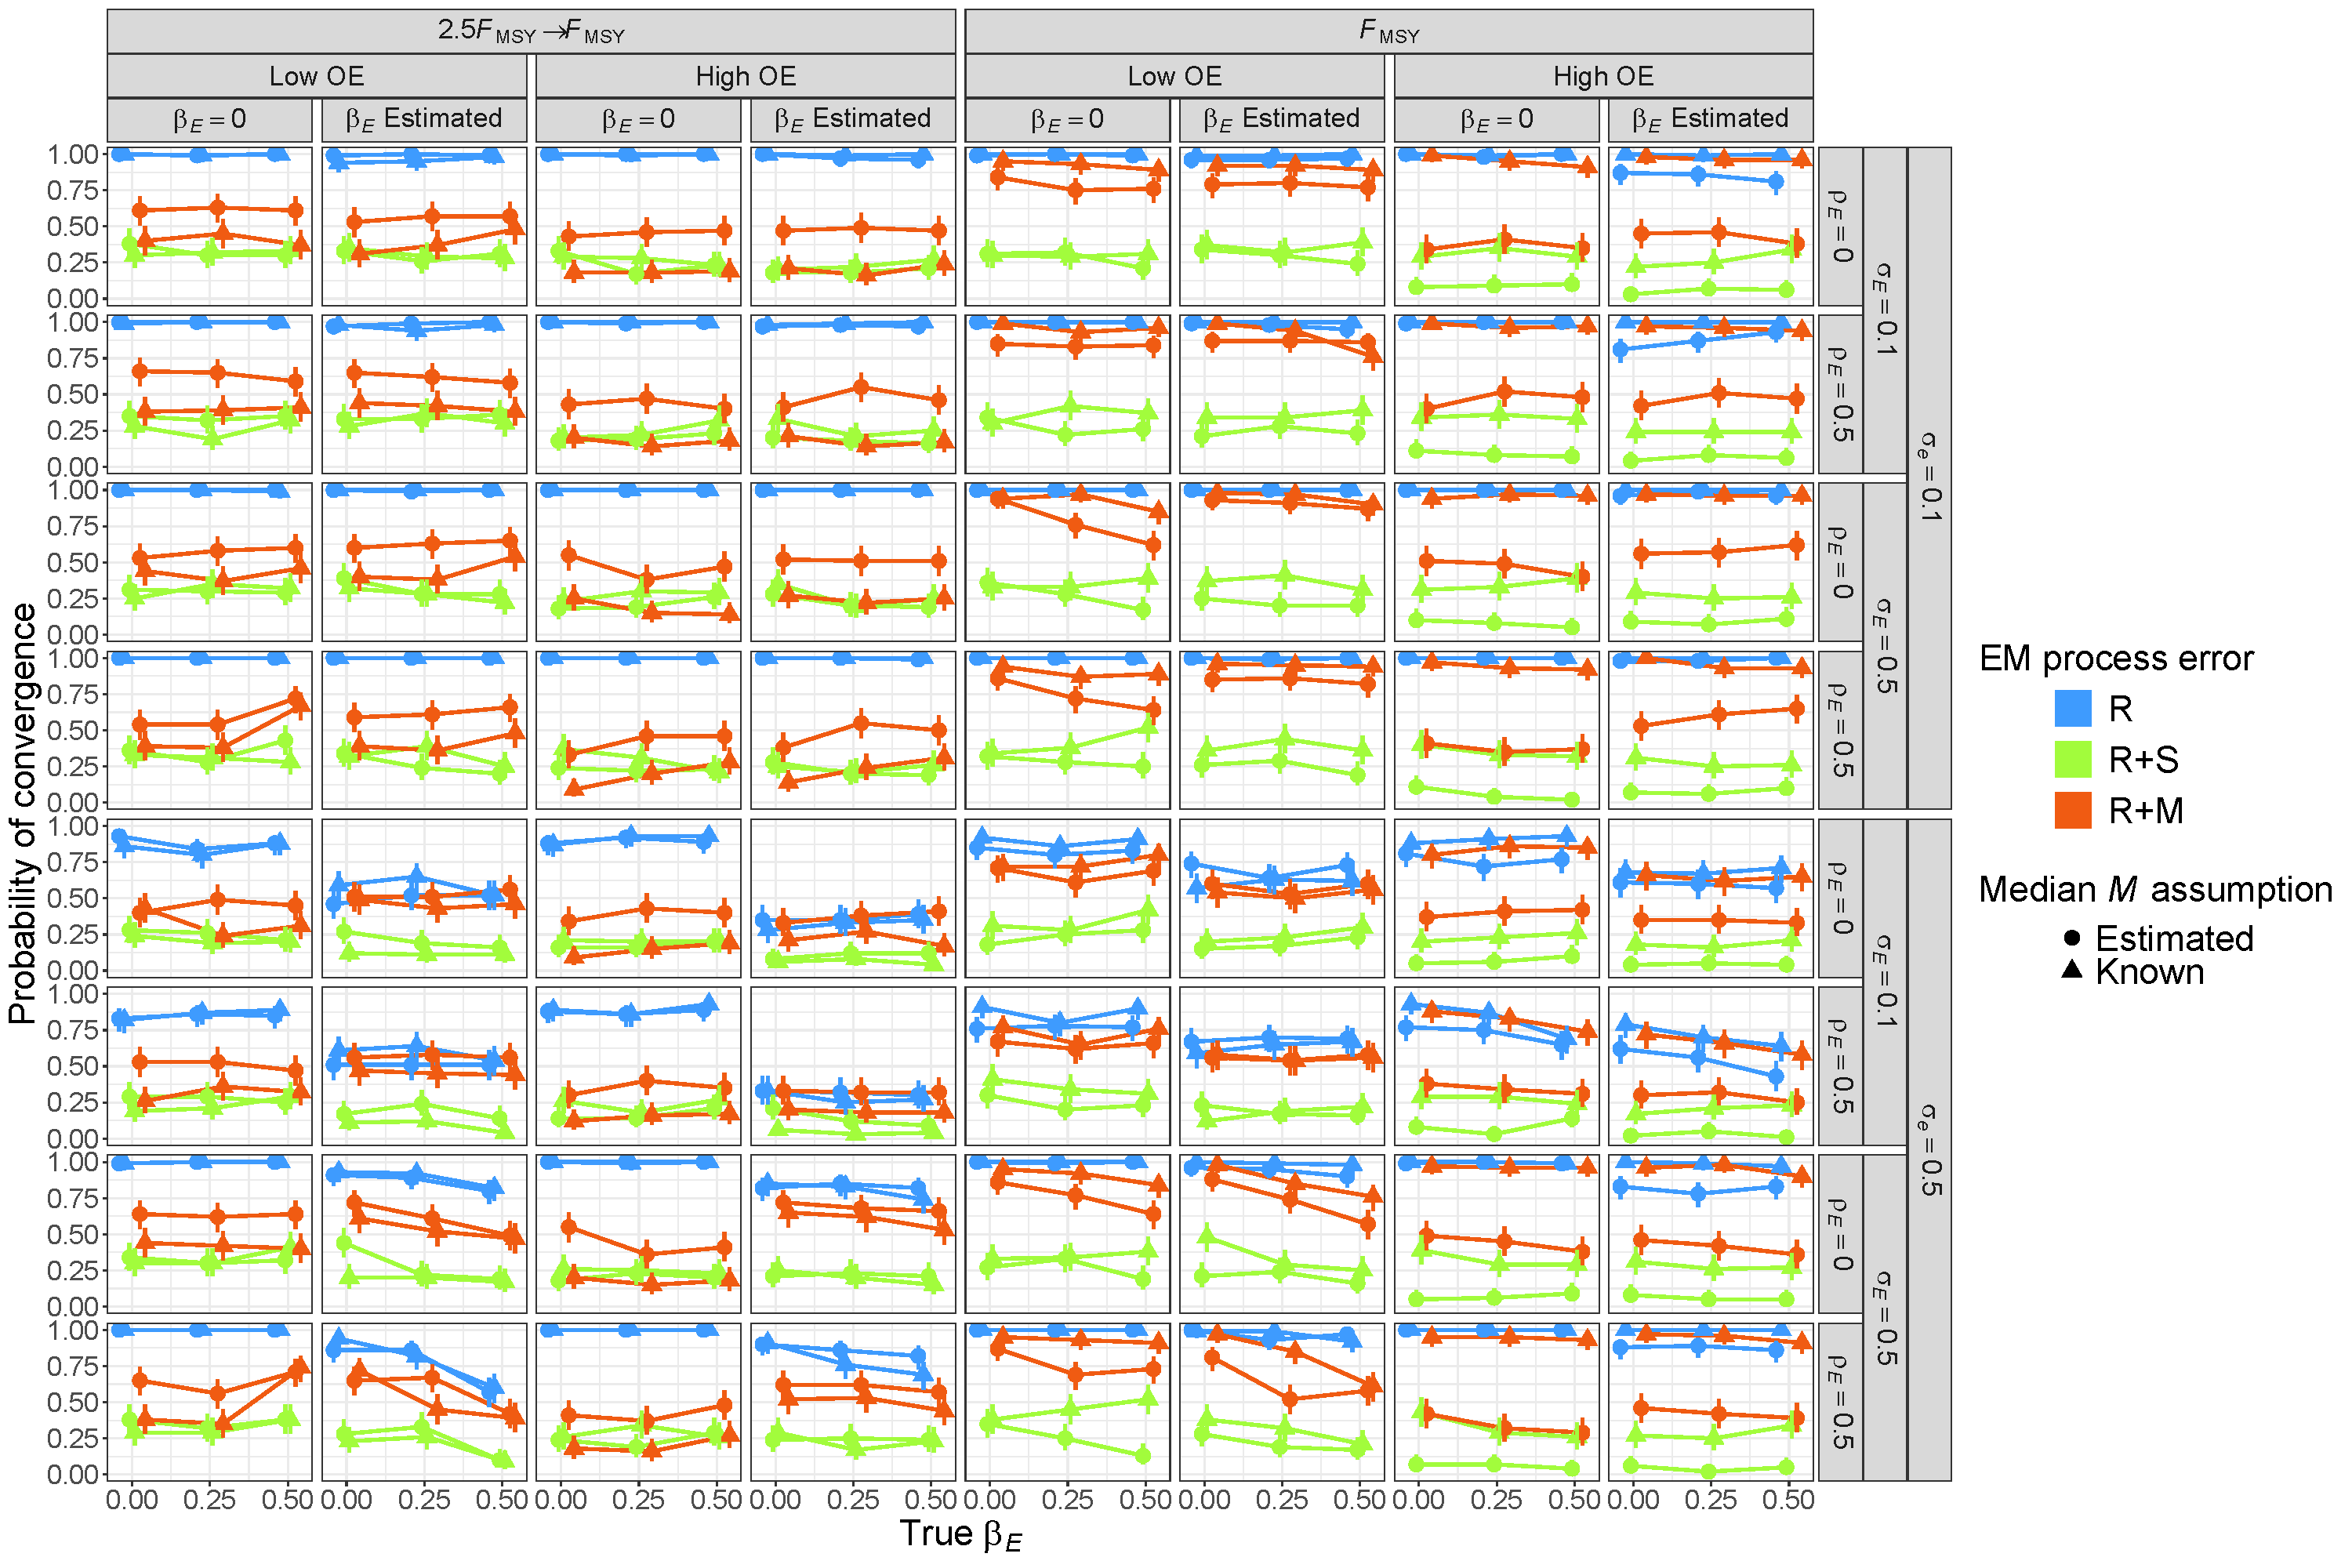
\includegraphics[height = \textheight]{convergence_Rom}
%DIFDELCMD < \end{center}
%DIFDELCMD < %%%
%DIFDELCMD < \caption{%
{%DIFAUXCMD
\DIFdelFL{Estimated probability of fits providing Hessian-based standard errors for EMs assuming alternative process error, that estimate or assume known median $M$, and that estimate or assume no covariate effect on median $M$ when fitted to R OMs and three levels of true covariate effect on median $M$ (x axis). Vertical lines represent 95\% confidence intervals.}}%DIFAUXCMD
%DIFDELCMD < \label{convergence_Rom}
%DIFDELCMD < \end{figure}
%DIFDELCMD < \end{landscape}
%DIFDELCMD < 

%DIFDELCMD < \begin{landscape}
%DIFDELCMD < \begin{figure}
%DIFDELCMD < \begin{center}
%DIFDELCMD < 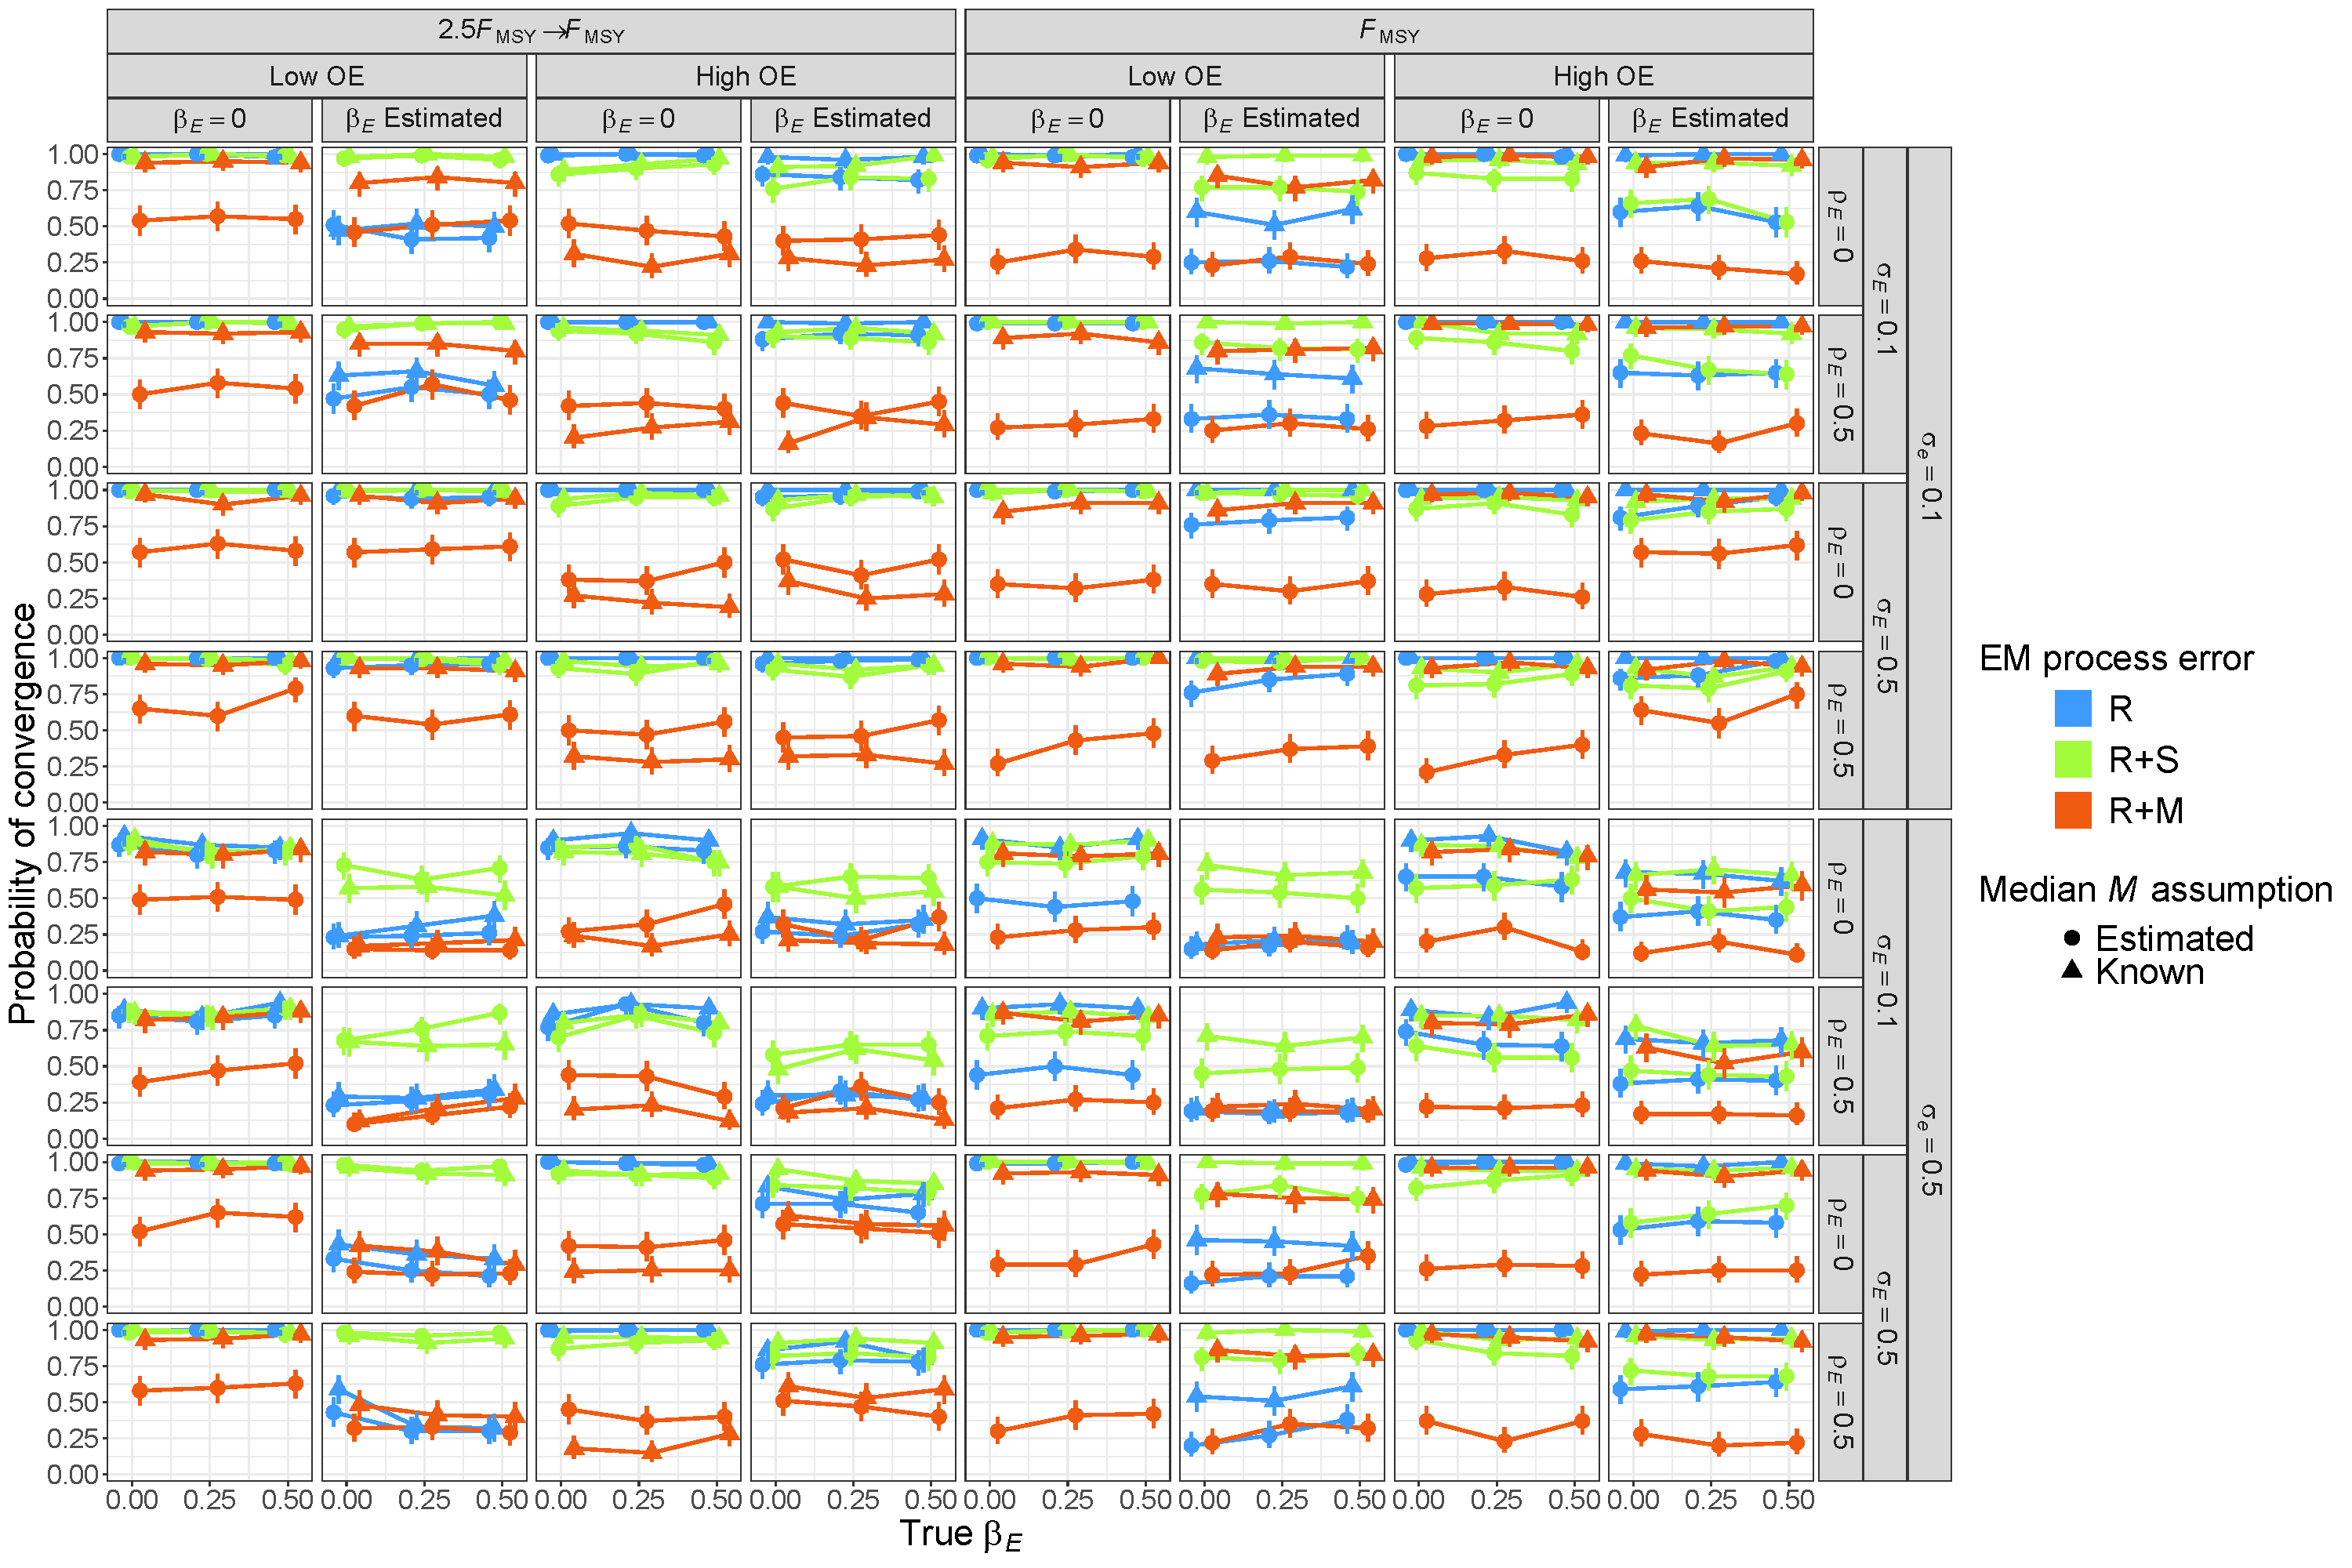
\includegraphics[height = \textheight]{convergence_RSom}
%DIFDELCMD < \end{center}
%DIFDELCMD < %%%
%DIFDELCMD < \caption{%
{%DIFAUXCMD
\DIFdelFL{Estimated probability of fits providing Hessian-based standard errors for EMs assuming alternative process error, that estimate or assume known median $M$, and that estimate or assume no covariate effect on median $M$ when fitted to R+S OMs and three levels of true covariate effect on median $M$ (x axis). Vertical lines represent 95\% confidence intervals.}}%DIFAUXCMD
%DIFDELCMD < \label{convergence_RSom}
%DIFDELCMD < \end{figure}
%DIFDELCMD < \end{landscape}
%DIFDELCMD < 

%DIFDELCMD < \begin{landscape}
%DIFDELCMD < \begin{figure}
%DIFDELCMD < \begin{center}
%DIFDELCMD < 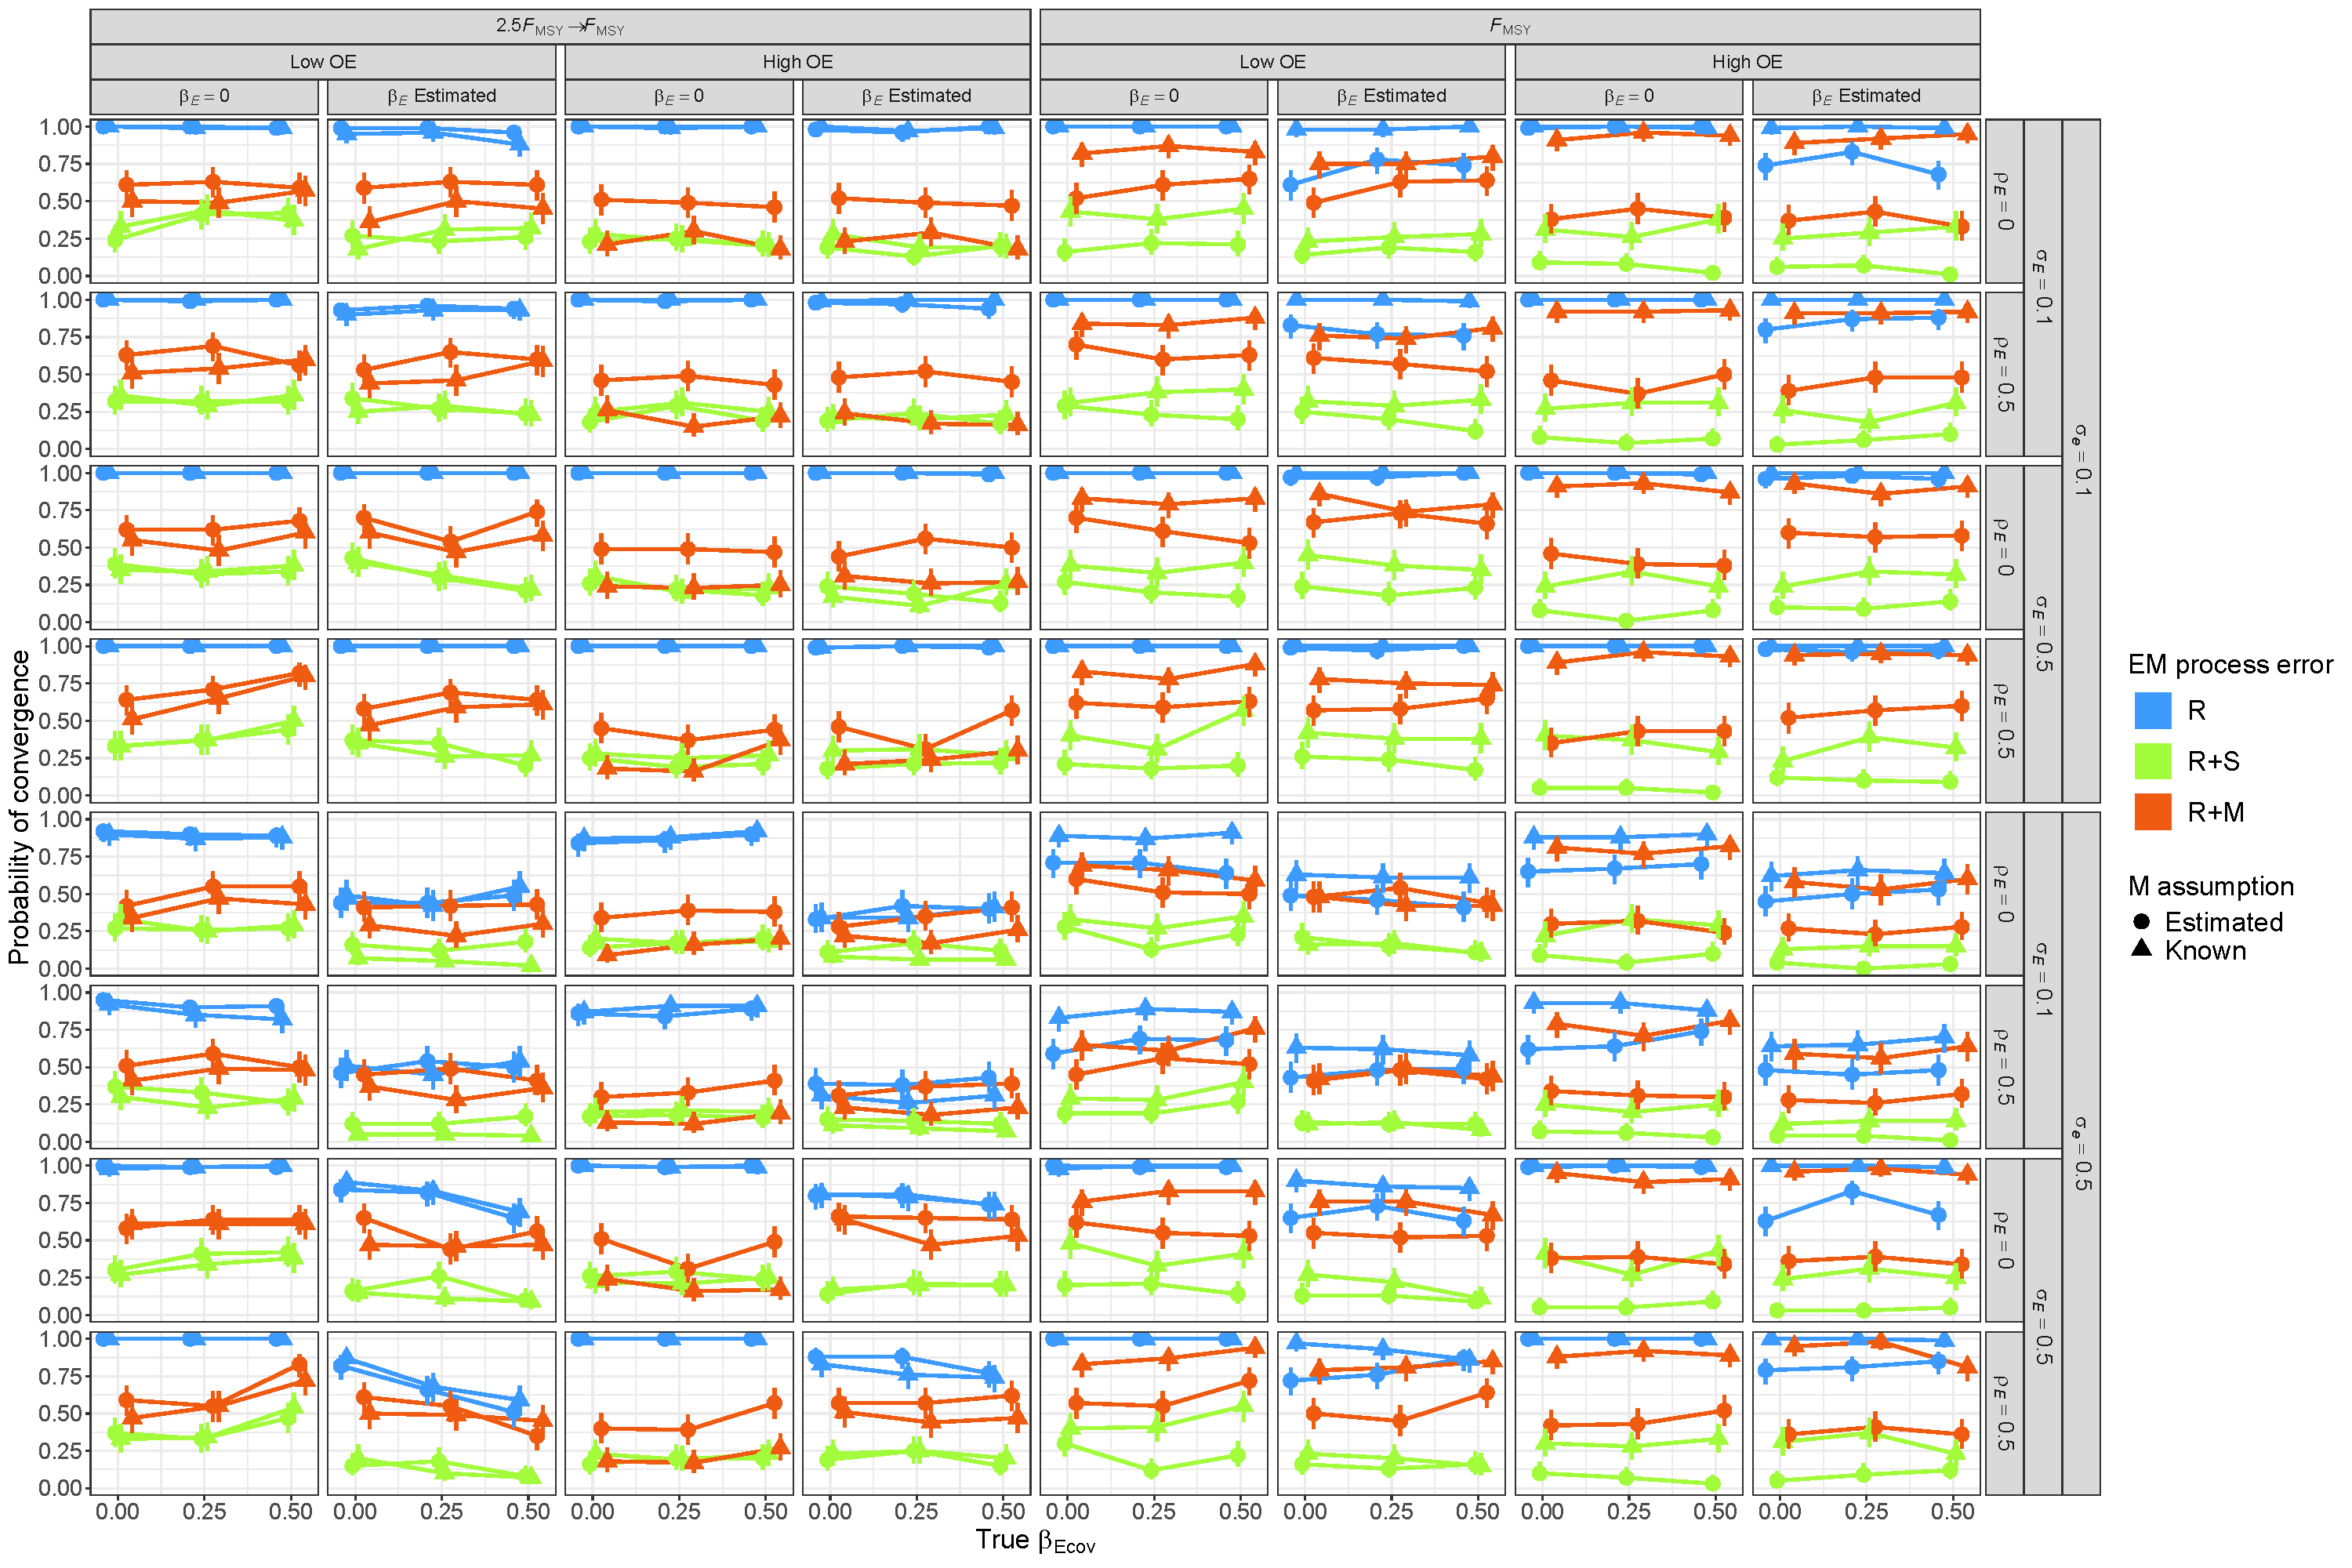
\includegraphics[height = \textheight]{convergence_RMom}
%DIFDELCMD < \end{center}
%DIFDELCMD < %%%
%DIFDELCMD < \caption{%
{%DIFAUXCMD
\DIFdelFL{Estimated probability of fits providing Hessian-based standard errors for EMs assuming alternative process error, that estimate or assume known median $M$, and that estimate or assume no covariate effect on median $M$ when fitted to R+M OMs and three levels of true covariate effect on median $M$ (x axis). Vertical lines represent 95\% confidence intervals.}}%DIFAUXCMD
%DIFDELCMD < \label{convergence_RMom}
%DIFDELCMD < \end{figure}
%DIFDELCMD < \end{landscape}
%DIFDELCMD < 

%DIFDELCMD < %%%
\subsection*{\DIFdel{AIC results}}%DIFAUXCMD
%DIFDELCMD < \label{aic-results}
%DIFDELCMD < %%%
\addcontentsline{toc}{subsection}{\DIFdel{AIC results}}
%DIFAUXCMD
%DIFDELCMD < 

%DIFDELCMD < \begin{landscape}
%DIFDELCMD < \begin{figure}
%DIFDELCMD < \begin{center}
%DIFDELCMD < 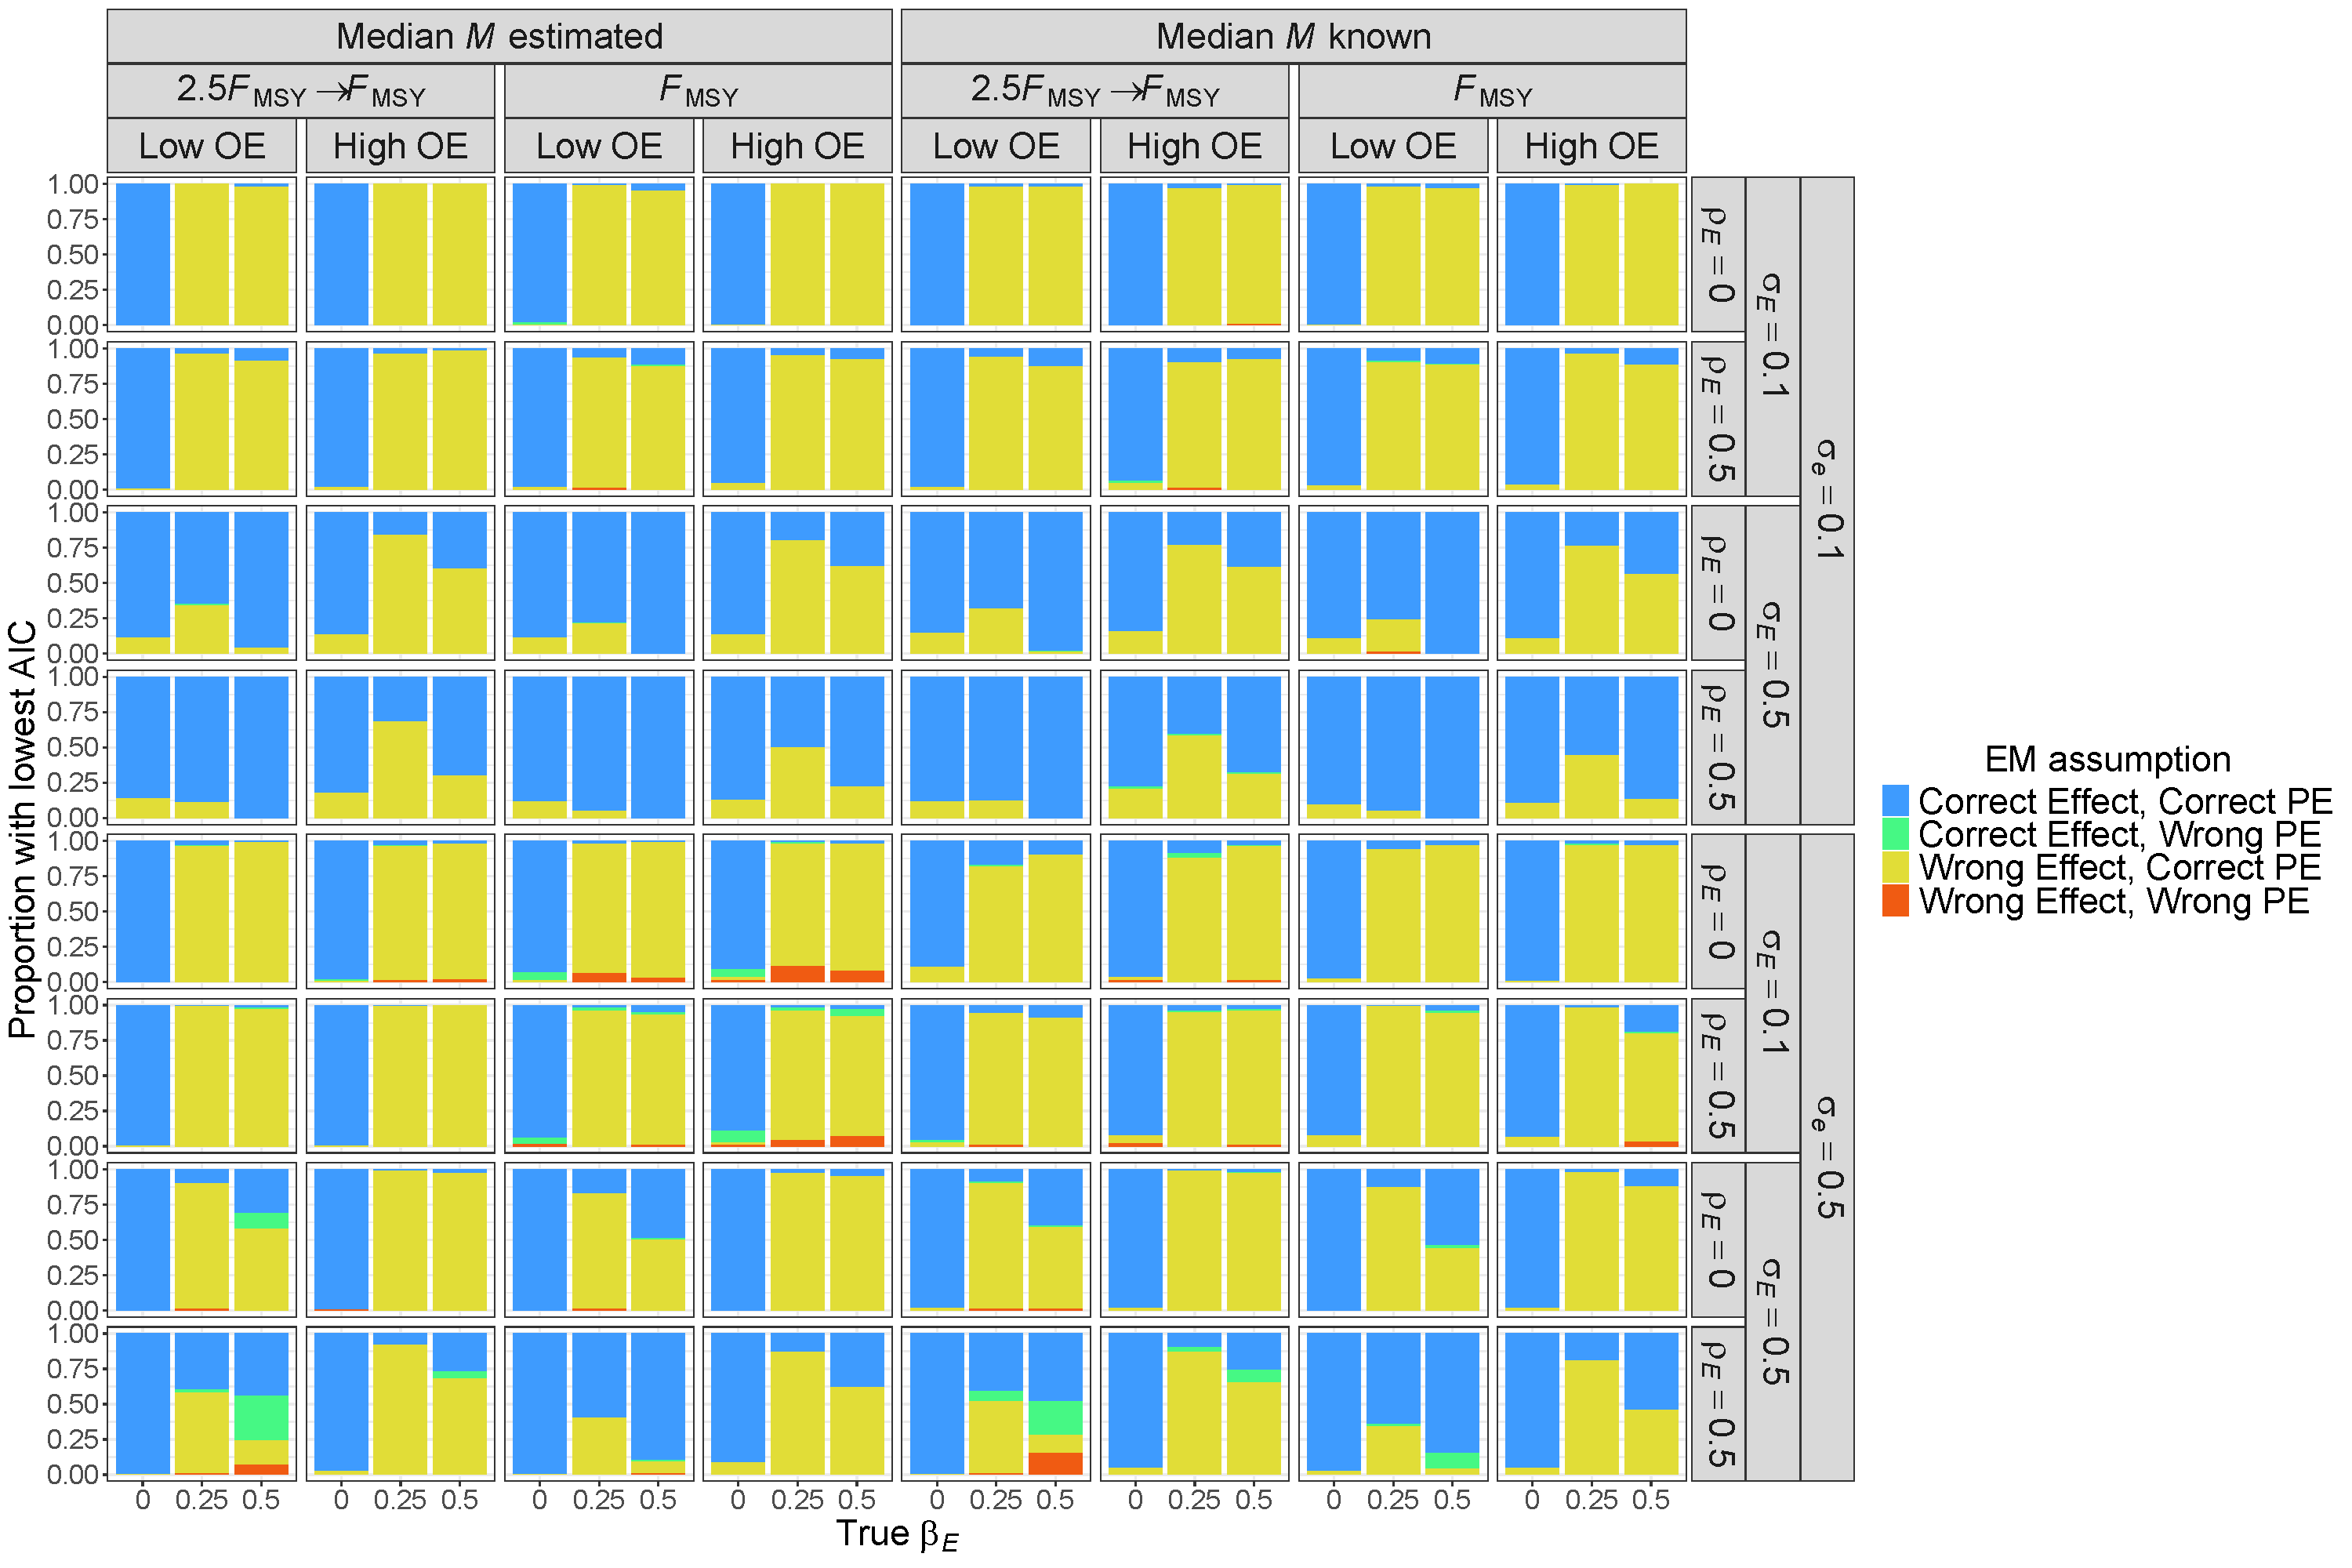
\includegraphics[height = \textheight]{aic_Rom}
%DIFDELCMD < \end{center}
%DIFDELCMD < %%%
%DIFDELCMD < \caption{%
{%DIFAUXCMD
\DIFdelFL{Proportion of simulated data sets for R OMs where the EM type (treatment of environmental covariate and assumed process error type) had the lowest AIC.}}%DIFAUXCMD
%DIFDELCMD < \label{aic_Rom}
%DIFDELCMD < \end{figure}
%DIFDELCMD < \end{landscape}
%DIFDELCMD < 

%DIFDELCMD < \begin{landscape}
%DIFDELCMD < \begin{figure}
%DIFDELCMD < \begin{center}
%DIFDELCMD < 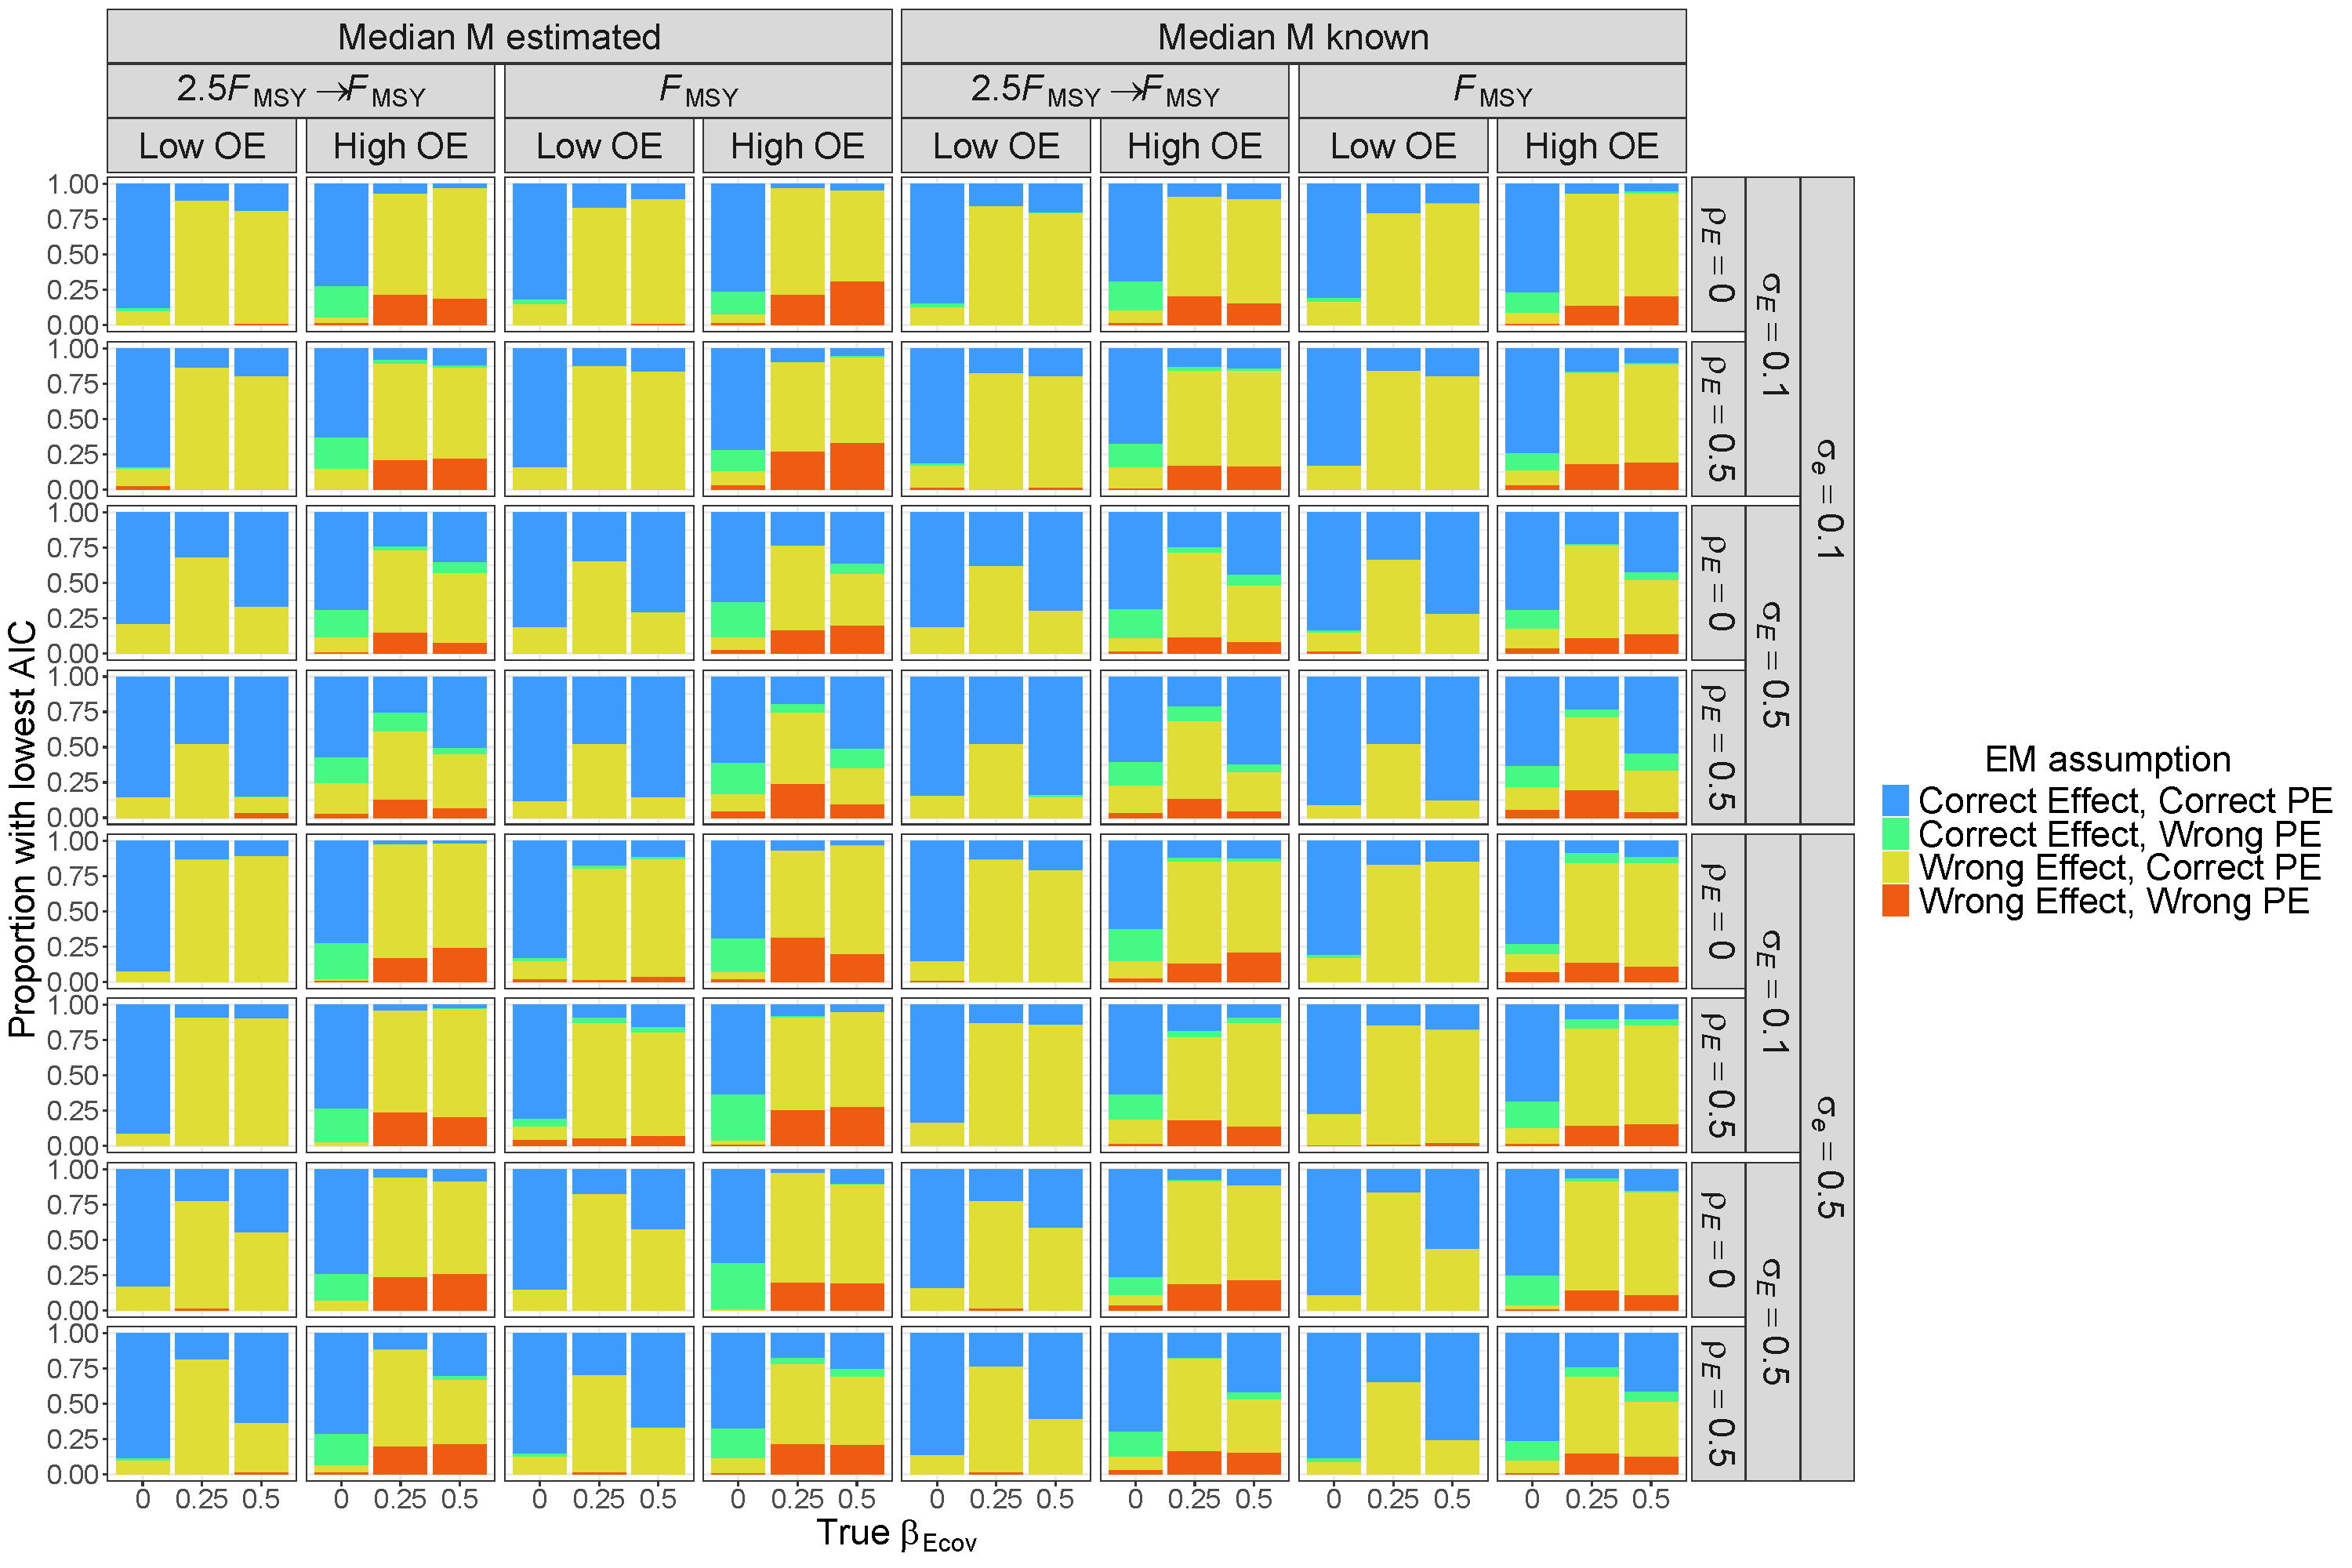
\includegraphics[height = \textheight]{aic_RSom}
%DIFDELCMD < \end{center}
%DIFDELCMD < %%%
%DIFDELCMD < \caption{%
{%DIFAUXCMD
\DIFdelFL{Proportion of simulated data sets for R+S OMs where the EM type (treatment of environmental covariate and assumed process error type) had the lowest AIC.}}%DIFAUXCMD
%DIFDELCMD < \label{aic_RSom}
%DIFDELCMD < \end{figure}
%DIFDELCMD < \end{landscape}
%DIFDELCMD < 

%DIFDELCMD < \begin{landscape}
%DIFDELCMD < \begin{figure}
%DIFDELCMD < \begin{center}
%DIFDELCMD < 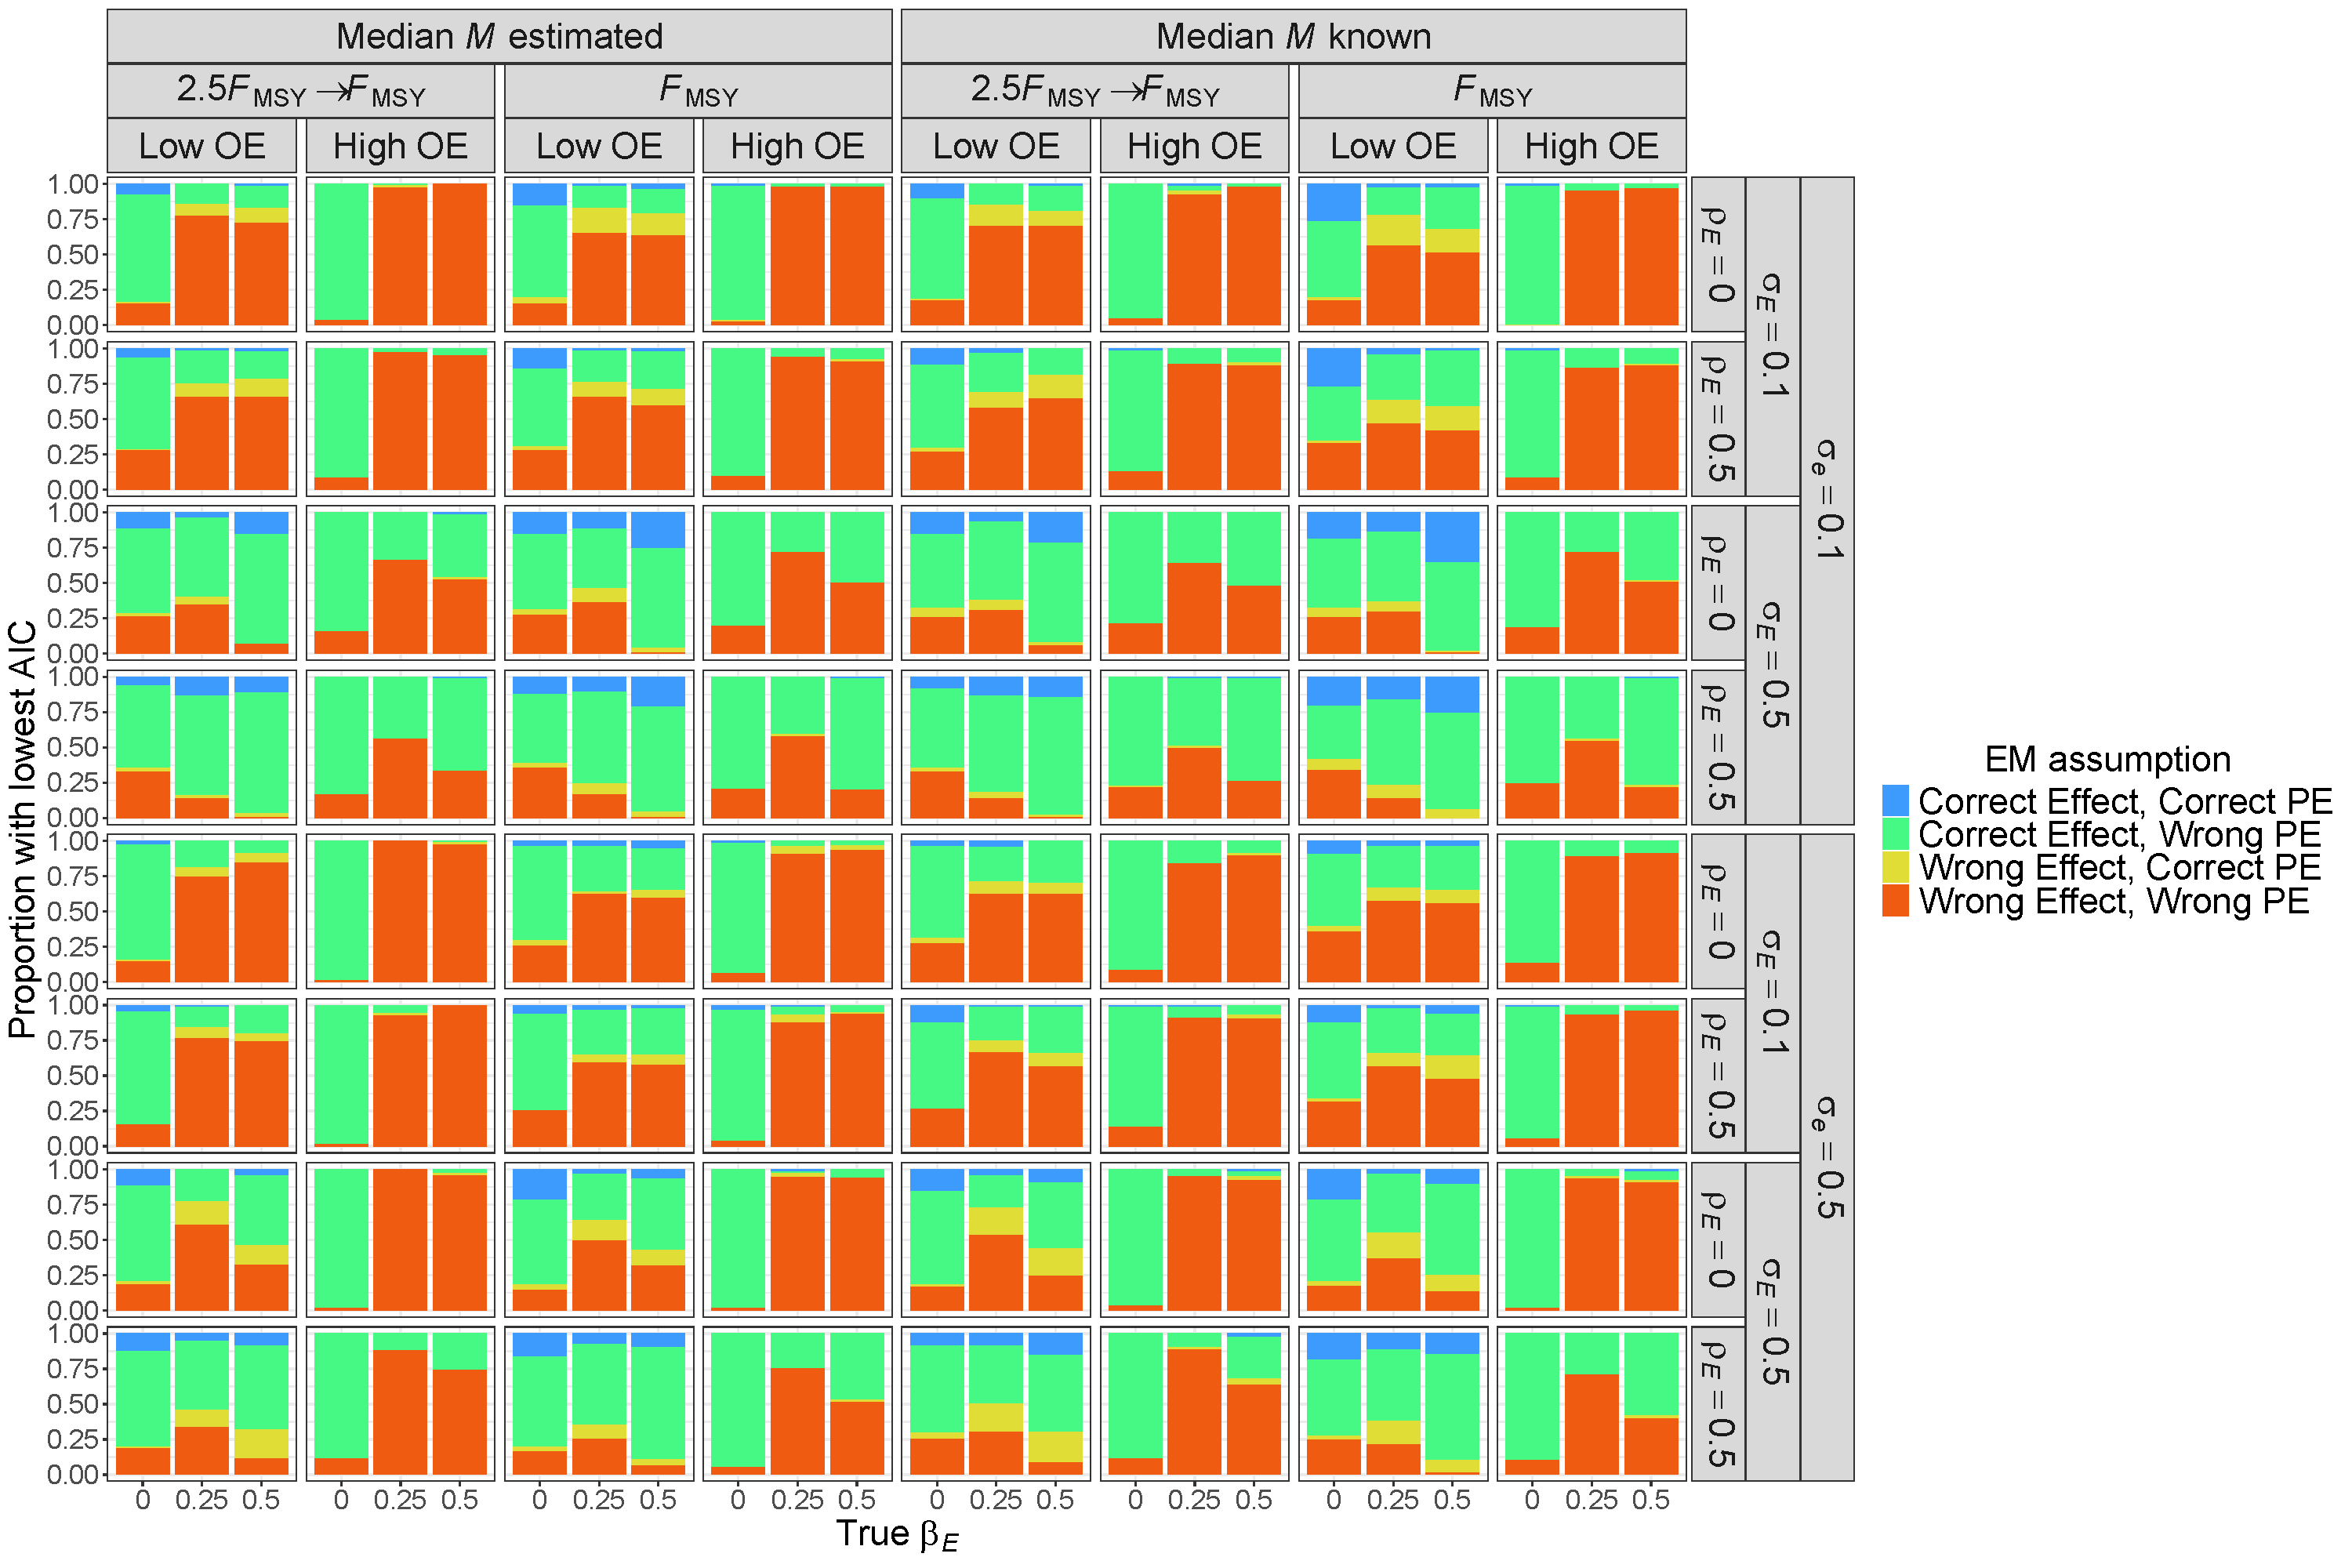
\includegraphics[height = \textheight]{aic_RMom}
%DIFDELCMD < \end{center}
%DIFDELCMD < %%%
%DIFDELCMD < \caption{%
{%DIFAUXCMD
\DIFdelFL{Proportion of simulated data sets for R+M OMs where the EM type (treatment of environmental covariate and assumed process error type) had the lowest AIC.}}%DIFAUXCMD
%DIFDELCMD < \label{aic_RMom}
%DIFDELCMD < \end{figure}
%DIFDELCMD < \end{landscape}
%DIFDELCMD < 

%DIFDELCMD < %%%
\subsection*{\DIFdel{Covariate effect bias}}%DIFAUXCMD
%DIFDELCMD < \label{covariate-effect-bias}
%DIFDELCMD < %%%
\addcontentsline{toc}{subsection}{\DIFdel{Covariate effect bias}}
%DIFAUXCMD
%DIFDELCMD < 

%DIFDELCMD < \begin{table}
%DIFDELCMD < %%%
%DIFDELCMD < \caption{%
{%DIFAUXCMD
\DIFdelFL{Percent reduction in deviance for linear regression models fit to errors in estimation of the covariate effect on $M$ ($\beta_E$). Table rows give each operating model (OM) and estimating model (EM) factor included individually, combined, and with second and third order interactions. Table columns are operating models (OMs) with process error on recruitment only (R), recruitment and apparent survival (R+S), or recruitment and natural mortality (R+M).}}%DIFAUXCMD
%DIFDELCMD < \label{bias_ecov_beta_complete_PRD_table}
%DIFDELCMD < {\begin{center}
%DIFDELCMD < \begin{tabular}{lrrr}
%DIFDELCMD < \hline\hline
%DIFDELCMD < %%%
%DIFDELCMD < \multicolumn{1}{l}{%
{%DIFAUXCMD
\DIFdelFL{Factor}}%DIFAUXCMD
%DIFDELCMD < &%%%
%DIFDELCMD < \multicolumn{1}{c}{%
{%DIFAUXCMD
\DIFdelFL{R}}%DIFAUXCMD
%DIFDELCMD < &%%%
%DIFDELCMD < \multicolumn{1}{c}{%
{%DIFAUXCMD
\DIFdelFL{R+S}}%DIFAUXCMD
%DIFDELCMD < &%%%
%DIFDELCMD < \multicolumn{1}{c}{%
{%DIFAUXCMD
\DIFdelFL{R+M}}%DIFAUXCMD
%DIFDELCMD < \tabularnewline
%DIFDELCMD < \hline
%DIFDELCMD < %%%
\DIFdelFL{OM }\DIFdelendFL $F$ history& \DIFdelbeginFL \DIFdelFL{\textless  0.01}\DIFdelendFL \DIFaddbeginFL \DIFaddFL{2.08}\DIFaddendFL & \DIFdelbeginFL \DIFdelFL{0.01}\DIFdelendFL \DIFaddbeginFL \DIFaddFL{2.74}\DIFaddendFL & \DIFdelbeginFL \DIFdelFL{\textless  0.01}\DIFdelendFL \DIFaddbeginFL \DIFaddFL{1.75}\DIFaddendFL \tabularnewline
OM Obs. Error& \DIFdelbeginFL \DIFdelFL{\textless  0.01}\DIFdelendFL \DIFaddbeginFL \DIFaddFL{1.09}\DIFaddendFL & \DIFdelbeginFL \DIFdelFL{\textless  0.01}\DIFdelendFL \DIFaddbeginFL \DIFaddFL{0.18}\DIFaddendFL & \DIFdelbeginFL \DIFdelFL{\textless  0.01}\DIFdelendFL \DIFaddbeginFL \DIFaddFL{1.19}\DIFaddendFL \tabularnewline
OM $\sigma_e$& \DIFdelbeginFL \DIFdelFL{\textless  }\DIFdelendFL 0.01&\textless  0.01&\textless  0.01\tabularnewline
OM $\sigma_E$&\textless  0.01&\textless  0.01&\textless  0.01\tabularnewline
OM $\rho_{E}$&\textless  0.01&\textless  0.01&\textless  0.01\tabularnewline
OM $\beta_{E}$&\textless  0.01& 0.01&\textless  0.01\tabularnewline
EM \DIFdelbeginFL \DIFdelFL{Convergence}\DIFdelendFL \DIFaddbeginFL \DIFaddFL{Process Error}\DIFaddendFL & \DIFdelbeginFL \DIFdelFL{\textless  0.01}\DIFdelendFL \DIFaddbeginFL \DIFaddFL{0.52}\DIFaddendFL & \DIFdelbeginFL \DIFdelFL{\textless  0.01}\DIFdelendFL \DIFaddbeginFL \DIFaddFL{1.05}\DIFaddendFL & \DIFdelbeginFL \DIFdelFL{\textless  0.01}\DIFdelendFL \DIFaddbeginFL \DIFaddFL{0.57}\DIFaddendFL \tabularnewline
EM \DIFdelbeginFL \DIFdelFL{Process Error}\DIFdelendFL \DIFaddbeginFL \DIFaddFL{$\beta_{E}$ assumption}\DIFaddendFL &\textless  0.01& \DIFdelbeginFL \DIFdelFL{0.01}\DIFdelendFL \DIFaddbeginFL \DIFaddFL{0.05}\DIFaddendFL & 0.01\tabularnewline
EM $M$ assumption& \DIFdelbeginFL \DIFdelFL{\textless  0.01}\DIFdelendFL \DIFaddbeginFL \DIFaddFL{1.76}\DIFaddendFL & \DIFdelbeginFL \DIFdelFL{\textless  0.01}\DIFdelendFL \DIFaddbeginFL \DIFaddFL{2.12}\DIFaddendFL & \DIFdelbeginFL \DIFdelFL{\textless  0.01}\DIFdelendFL \DIFaddbeginFL \DIFaddFL{1.51}\DIFaddendFL \tabularnewline
All factors& \DIFdelbeginFL \DIFdelFL{0.02}\DIFdelendFL \DIFaddbeginFL \DIFaddFL{5.97}\DIFaddendFL & \DIFdelbeginFL \DIFdelFL{0.03}\DIFdelendFL \DIFaddbeginFL \DIFaddFL{6.58}\DIFaddendFL & \DIFdelbeginFL \DIFdelFL{0.03}\DIFdelendFL \DIFaddbeginFL \DIFaddFL{5.21}\DIFaddendFL \tabularnewline
+ All Two Way&\DIFdelbeginFL \DIFdelFL{0.16}\DIFdelendFL \DIFaddbeginFL \DIFaddFL{12.81}\DIFaddendFL &\DIFdelbeginFL \DIFdelFL{0.20}\DIFdelendFL \DIFaddbeginFL \DIFaddFL{13.00}\DIFaddendFL &\DIFdelbeginFL \DIFdelFL{0.18}\DIFdelendFL \DIFaddbeginFL \DIFaddFL{11.97}\DIFaddendFL \tabularnewline
+ All Three Way&\DIFdelbeginFL \DIFdelFL{0.58}\DIFdelendFL \DIFaddbeginFL \DIFaddFL{16.41}\DIFaddendFL &\DIFdelbeginFL \DIFdelFL{0.73}\DIFdelendFL \DIFaddbeginFL \DIFaddFL{15.57}\DIFaddendFL &\DIFdelbeginFL \DIFdelFL{0.59}\DIFdelendFL \DIFaddbeginFL \DIFaddFL{15.73}\DIFaddendFL \tabularnewline
\hline
\end{tabular}\end{center}
}
\end{table}
\DIFaddbegin \pagebreak
\DIFaddend 

\DIFdelbegin %DIFDELCMD < \begin{landscape}
%DIFDELCMD < \begin{figure}
%DIFDELCMD < \begin{center}
%DIFDELCMD < 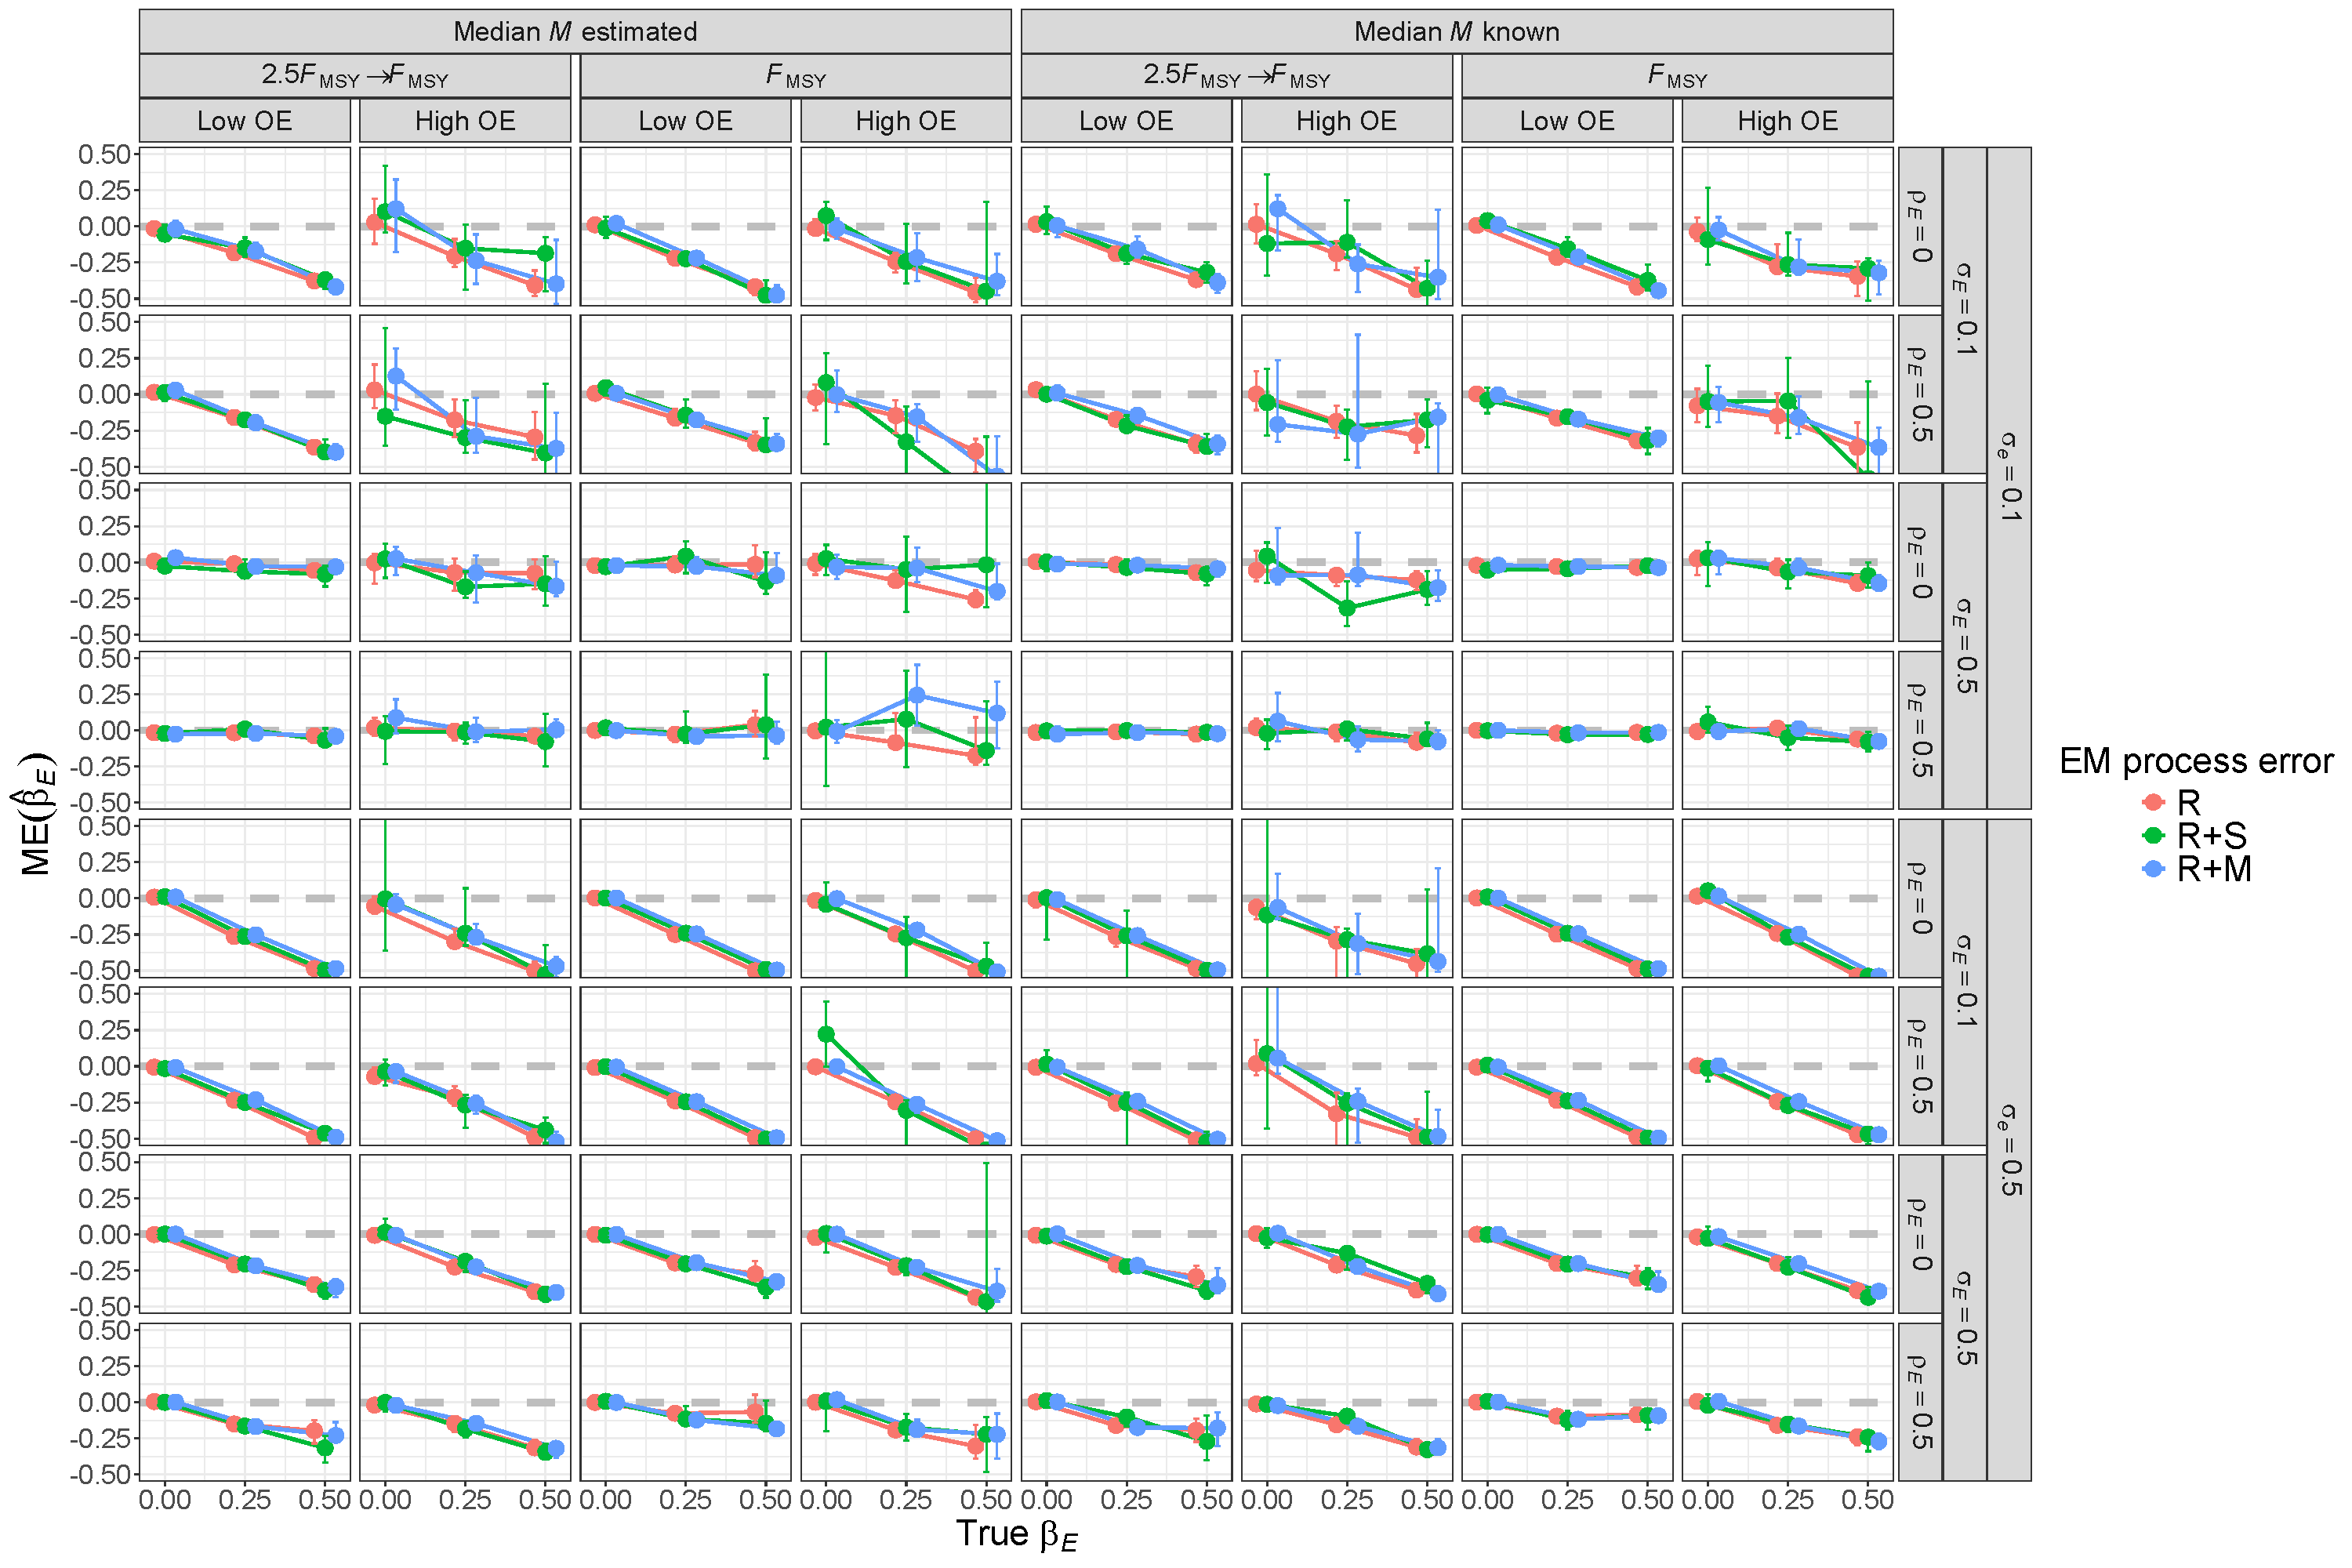
\includegraphics[height = \textheight]{beta_E_bias_Rom}
%DIFDELCMD < \end{center}
%DIFDELCMD < %%%
%DIFDELCMD < \caption{%
{%DIFAUXCMD
\DIFdelFL{For R OMs, median error (ME) of estimates of environmental effect on $M$ ($\beta_E$) from fitting EMs with alternative process error assumptions and treatment of median $M$ parameter ($\beta_M$). Vertical lines represent 95\% confidence intervals.}}%DIFAUXCMD
%DIFDELCMD < \label{beta_E_bias_Rom}
%DIFDELCMD < \end{figure}
%DIFDELCMD < \end{landscape}
%DIFDELCMD < 

%DIFDELCMD < \begin{landscape}
%DIFDELCMD < \begin{figure}
%DIFDELCMD < \begin{center}
%DIFDELCMD < 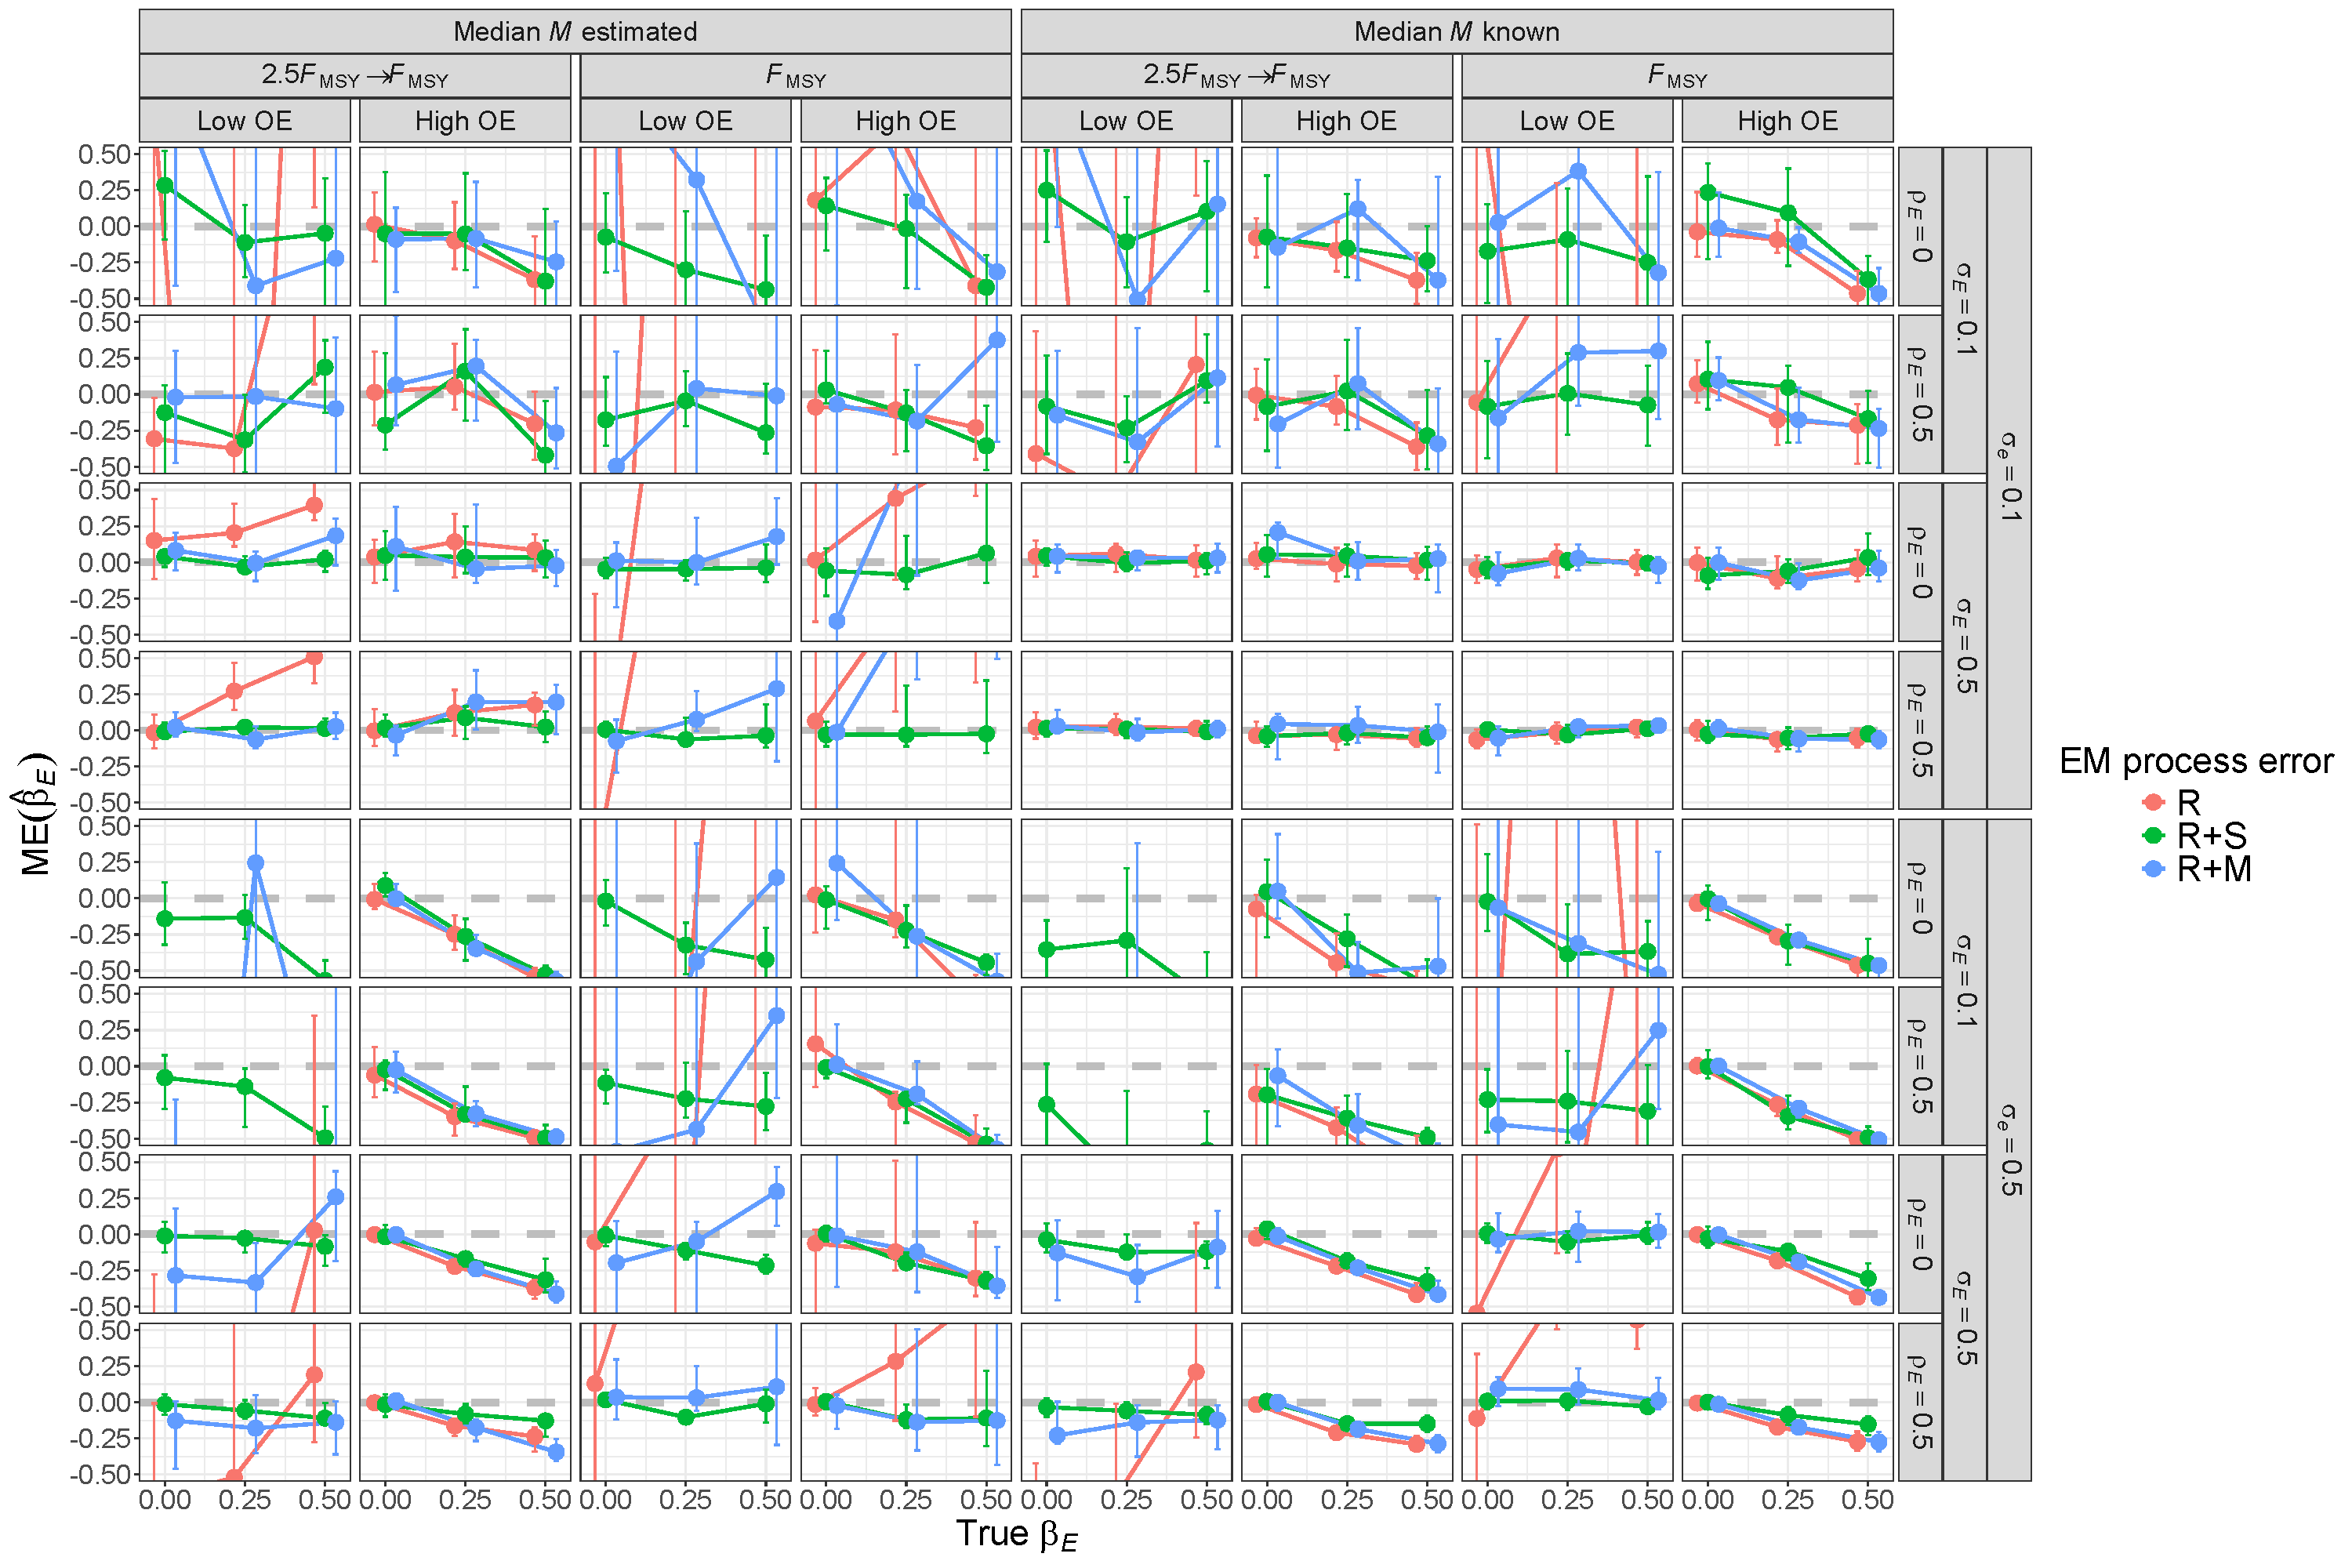
\includegraphics[height = \textheight]{beta_E_bias_RSom}
%DIFDELCMD < \end{center}
%DIFDELCMD < %%%
%DIFDELCMD < \caption{%
{%DIFAUXCMD
\DIFdelFL{For R+S OMs, median error (ME) of estimates of environmental effect on $M$ ($\beta_E$) from fitting EMs with alternative process error assumptions and treatment of median $M$ parameter ($\beta_M$). Vertical lines represent 95\% confidence intervals.}}%DIFAUXCMD
%DIFDELCMD < \label{beta_E_bias_RSom}
%DIFDELCMD < \end{figure}
%DIFDELCMD < \end{landscape}
%DIFDELCMD < 

%DIFDELCMD < \begin{landscape}
%DIFDELCMD < \begin{figure}
%DIFDELCMD < \begin{center}
%DIFDELCMD < 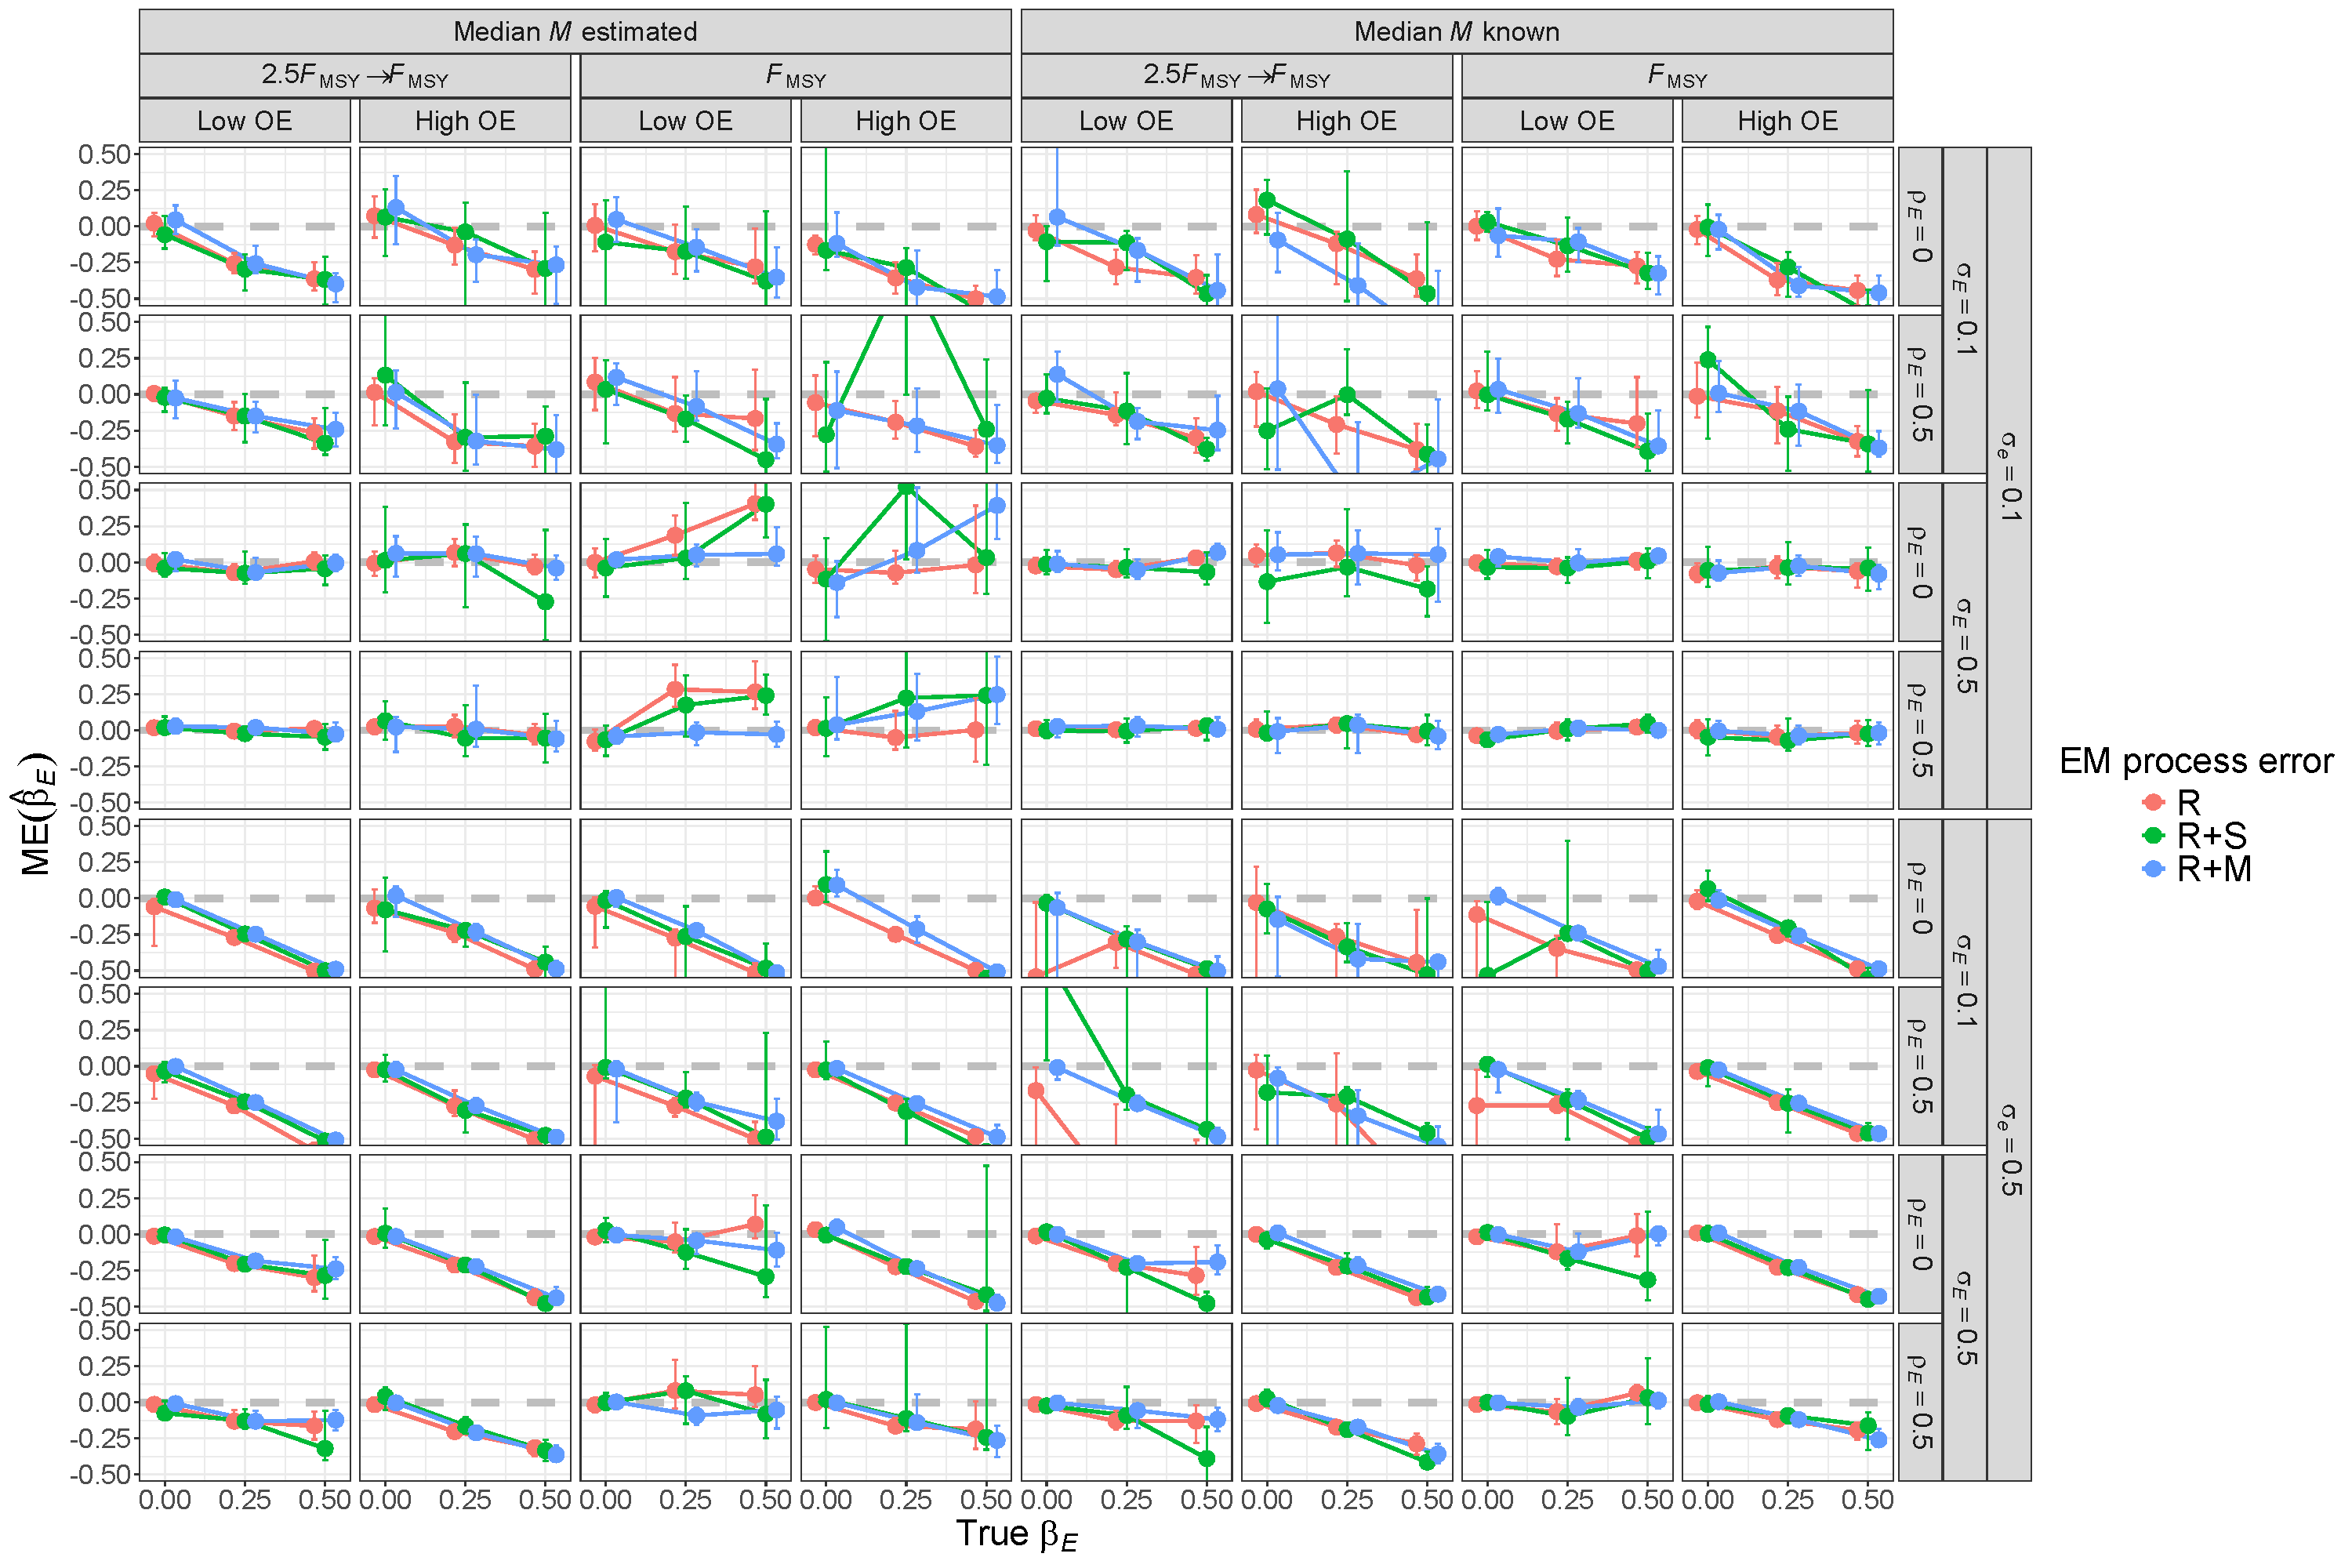
\includegraphics[height = \textheight]{beta_E_bias_RMom}
%DIFDELCMD < \end{center}
%DIFDELCMD < %%%
%DIFDELCMD < \caption{%
{%DIFAUXCMD
\DIFdelFL{For R+M OMs, median error (ME) of estimates of environmental effect on $M$ ($\beta_E$) from fitting EMs with alternative process error assumptions and treatment of median $M$ parameter ($\beta_M$). Vertical lines represent 95\% confidence intervals.}}%DIFAUXCMD
%DIFDELCMD < \label{beta_E_bias_RMom}
%DIFDELCMD < \end{figure}
%DIFDELCMD < \end{landscape}
%DIFDELCMD < 

%DIFDELCMD < %%%
\subsection*{\DIFdel{Covariate effect standard error estimation bias}}%DIFAUXCMD
%DIFDELCMD < \label{covariate-effect-standard-error-estimation-bias}
%DIFDELCMD < %%%
\addcontentsline{toc}{subsection}{\DIFdel{Covariate effect standard error estimation bias}}
%DIFAUXCMD
%DIFDELCMD < 

%DIFDELCMD < \begin{landscape}
%DIFDELCMD < \begin{figure}
%DIFDELCMD < \begin{center}
%DIFDELCMD < 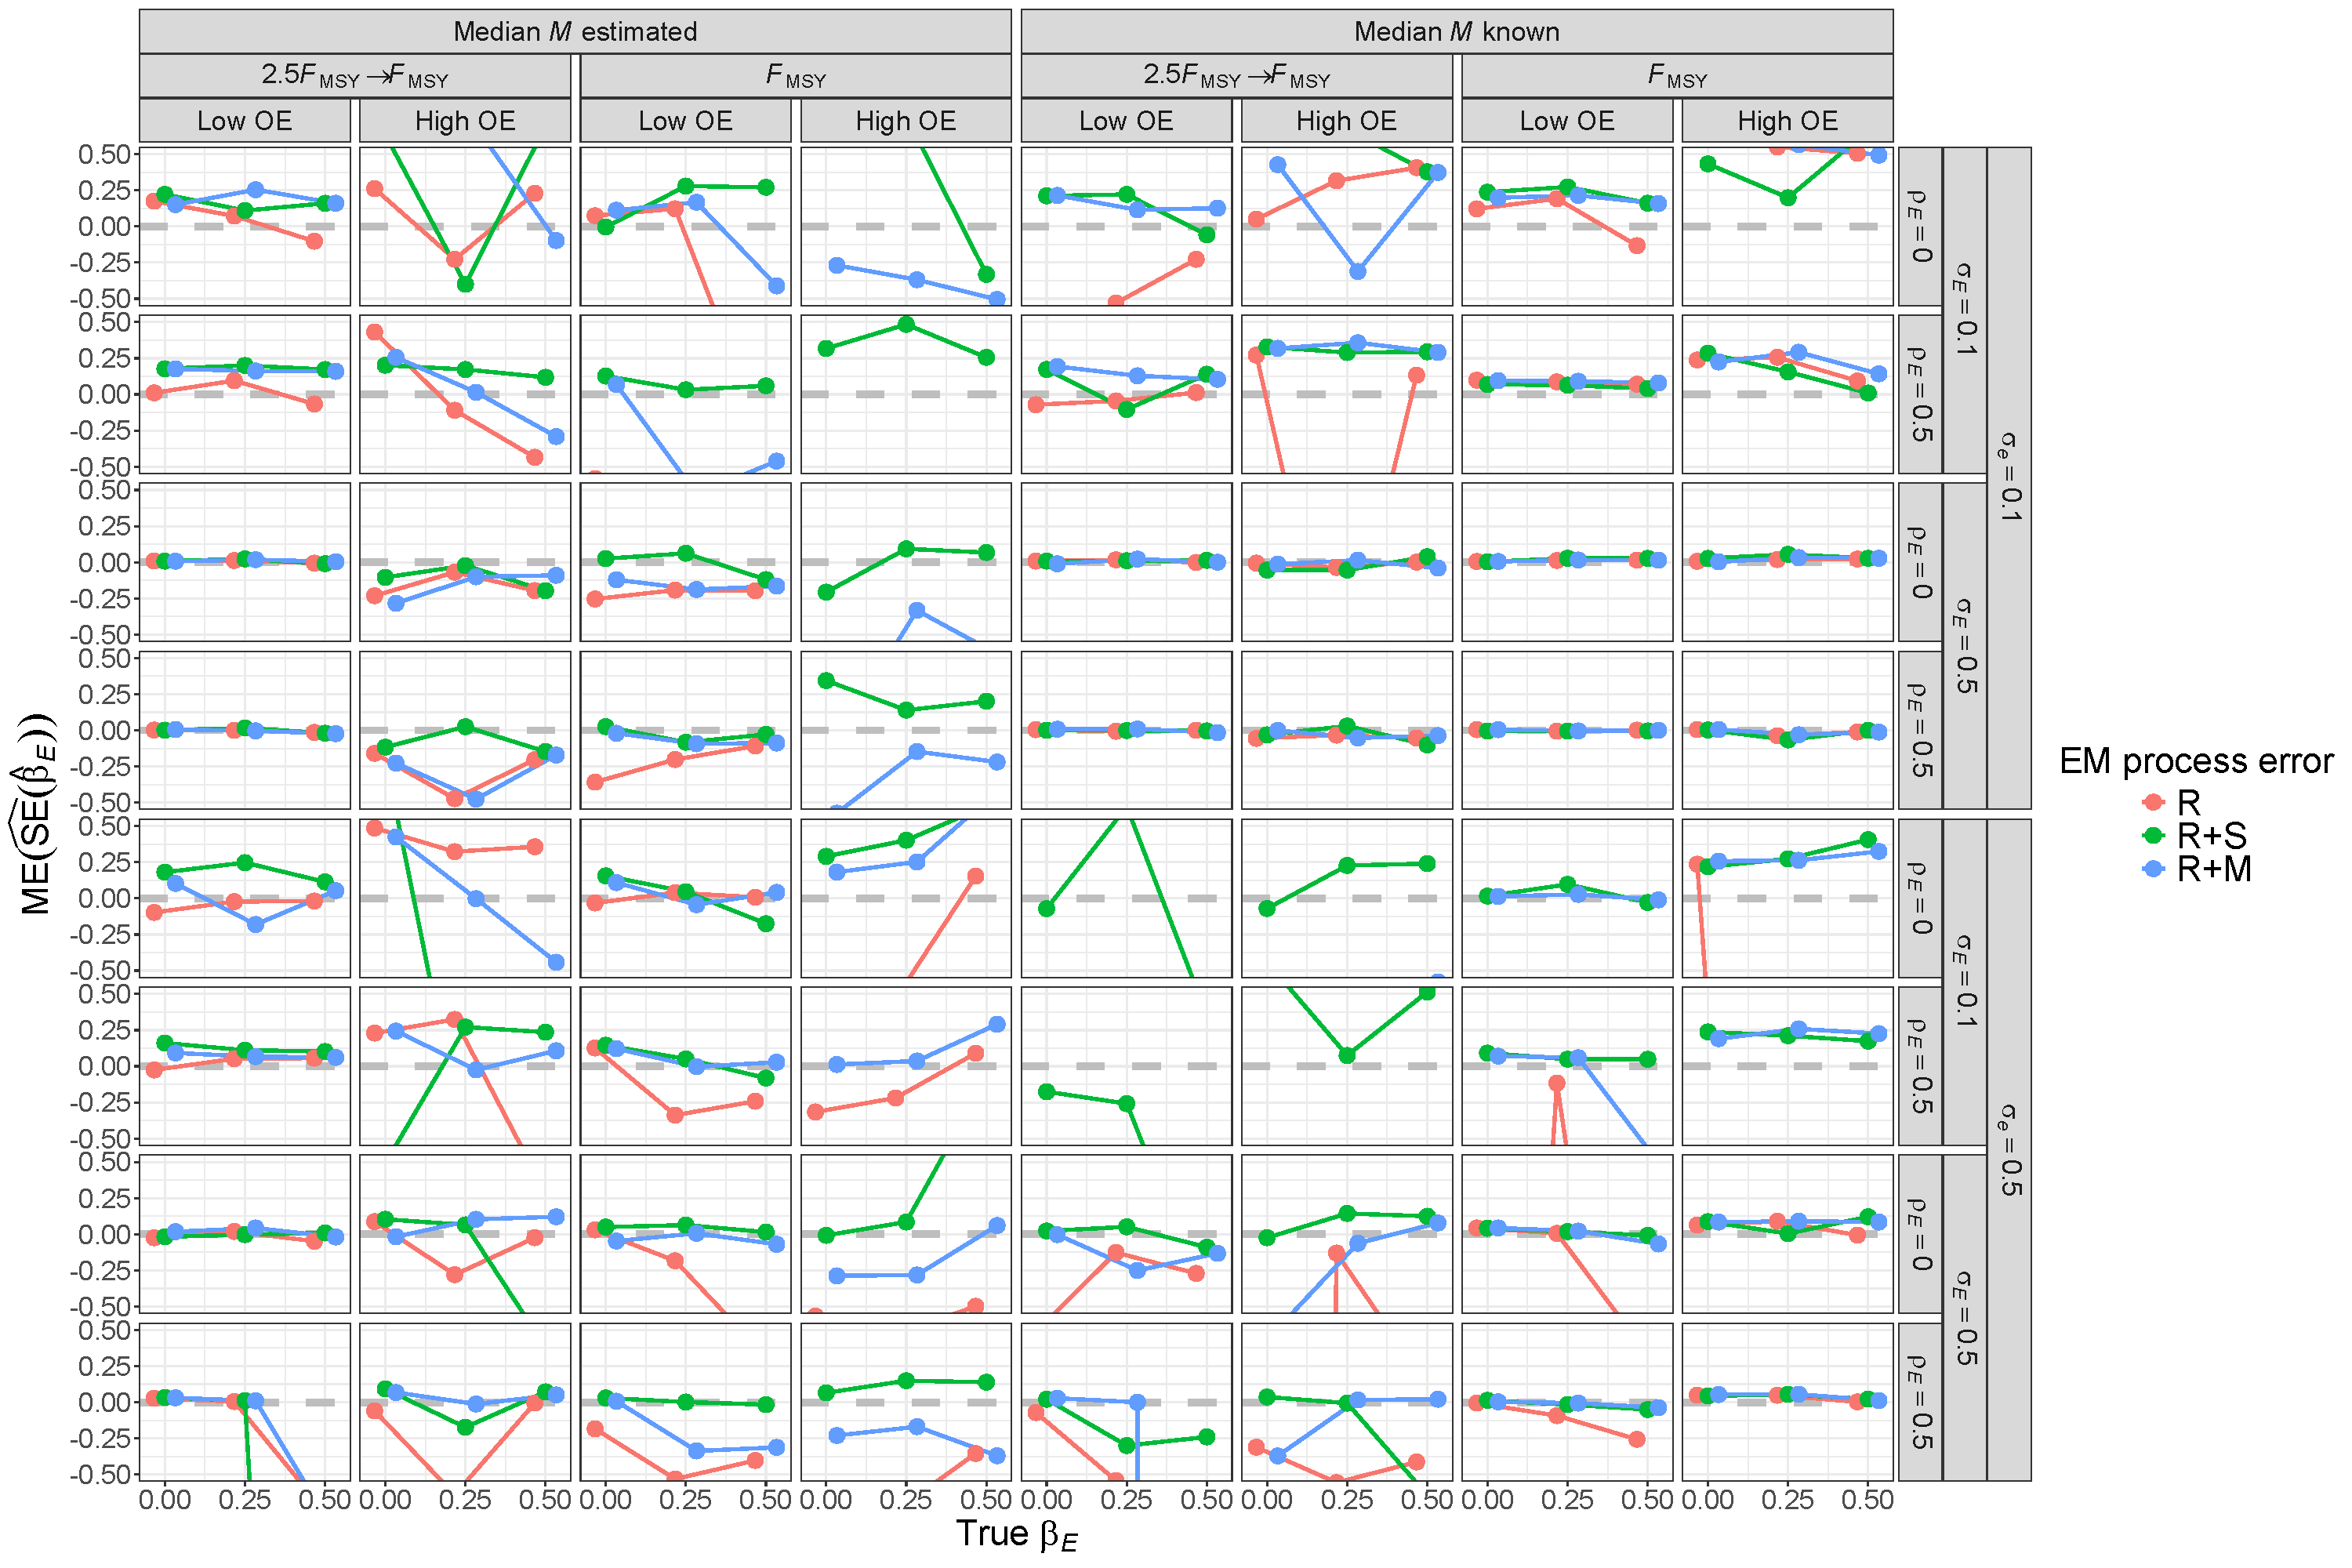
\includegraphics[height = \textheight]{se_beta_E_bias_Rom}
%DIFDELCMD < \end{center}
%DIFDELCMD < %%%
%DIFDELCMD < \caption{%
{%DIFAUXCMD
\DIFdelFL{For R OMs, median error (ME) of Hessian-based estimates of standard error for covariate effect on $M$ ($\beta_E$) from fitting EMs with alternative process error assumptions and treatment of median $M$ parameter ($\beta_M$). True standard error is defined as the mean of the standard error estimates accross converged fits to simulated data sets for a given OM scenario.}}%DIFAUXCMD
%DIFDELCMD < \label{se_beta_E_bias_Rom}
%DIFDELCMD < \end{figure}
%DIFDELCMD < \end{landscape}
%DIFDELCMD < 

%DIFDELCMD < \begin{landscape}
%DIFDELCMD < \begin{figure}
%DIFDELCMD < \begin{center}
%DIFDELCMD < 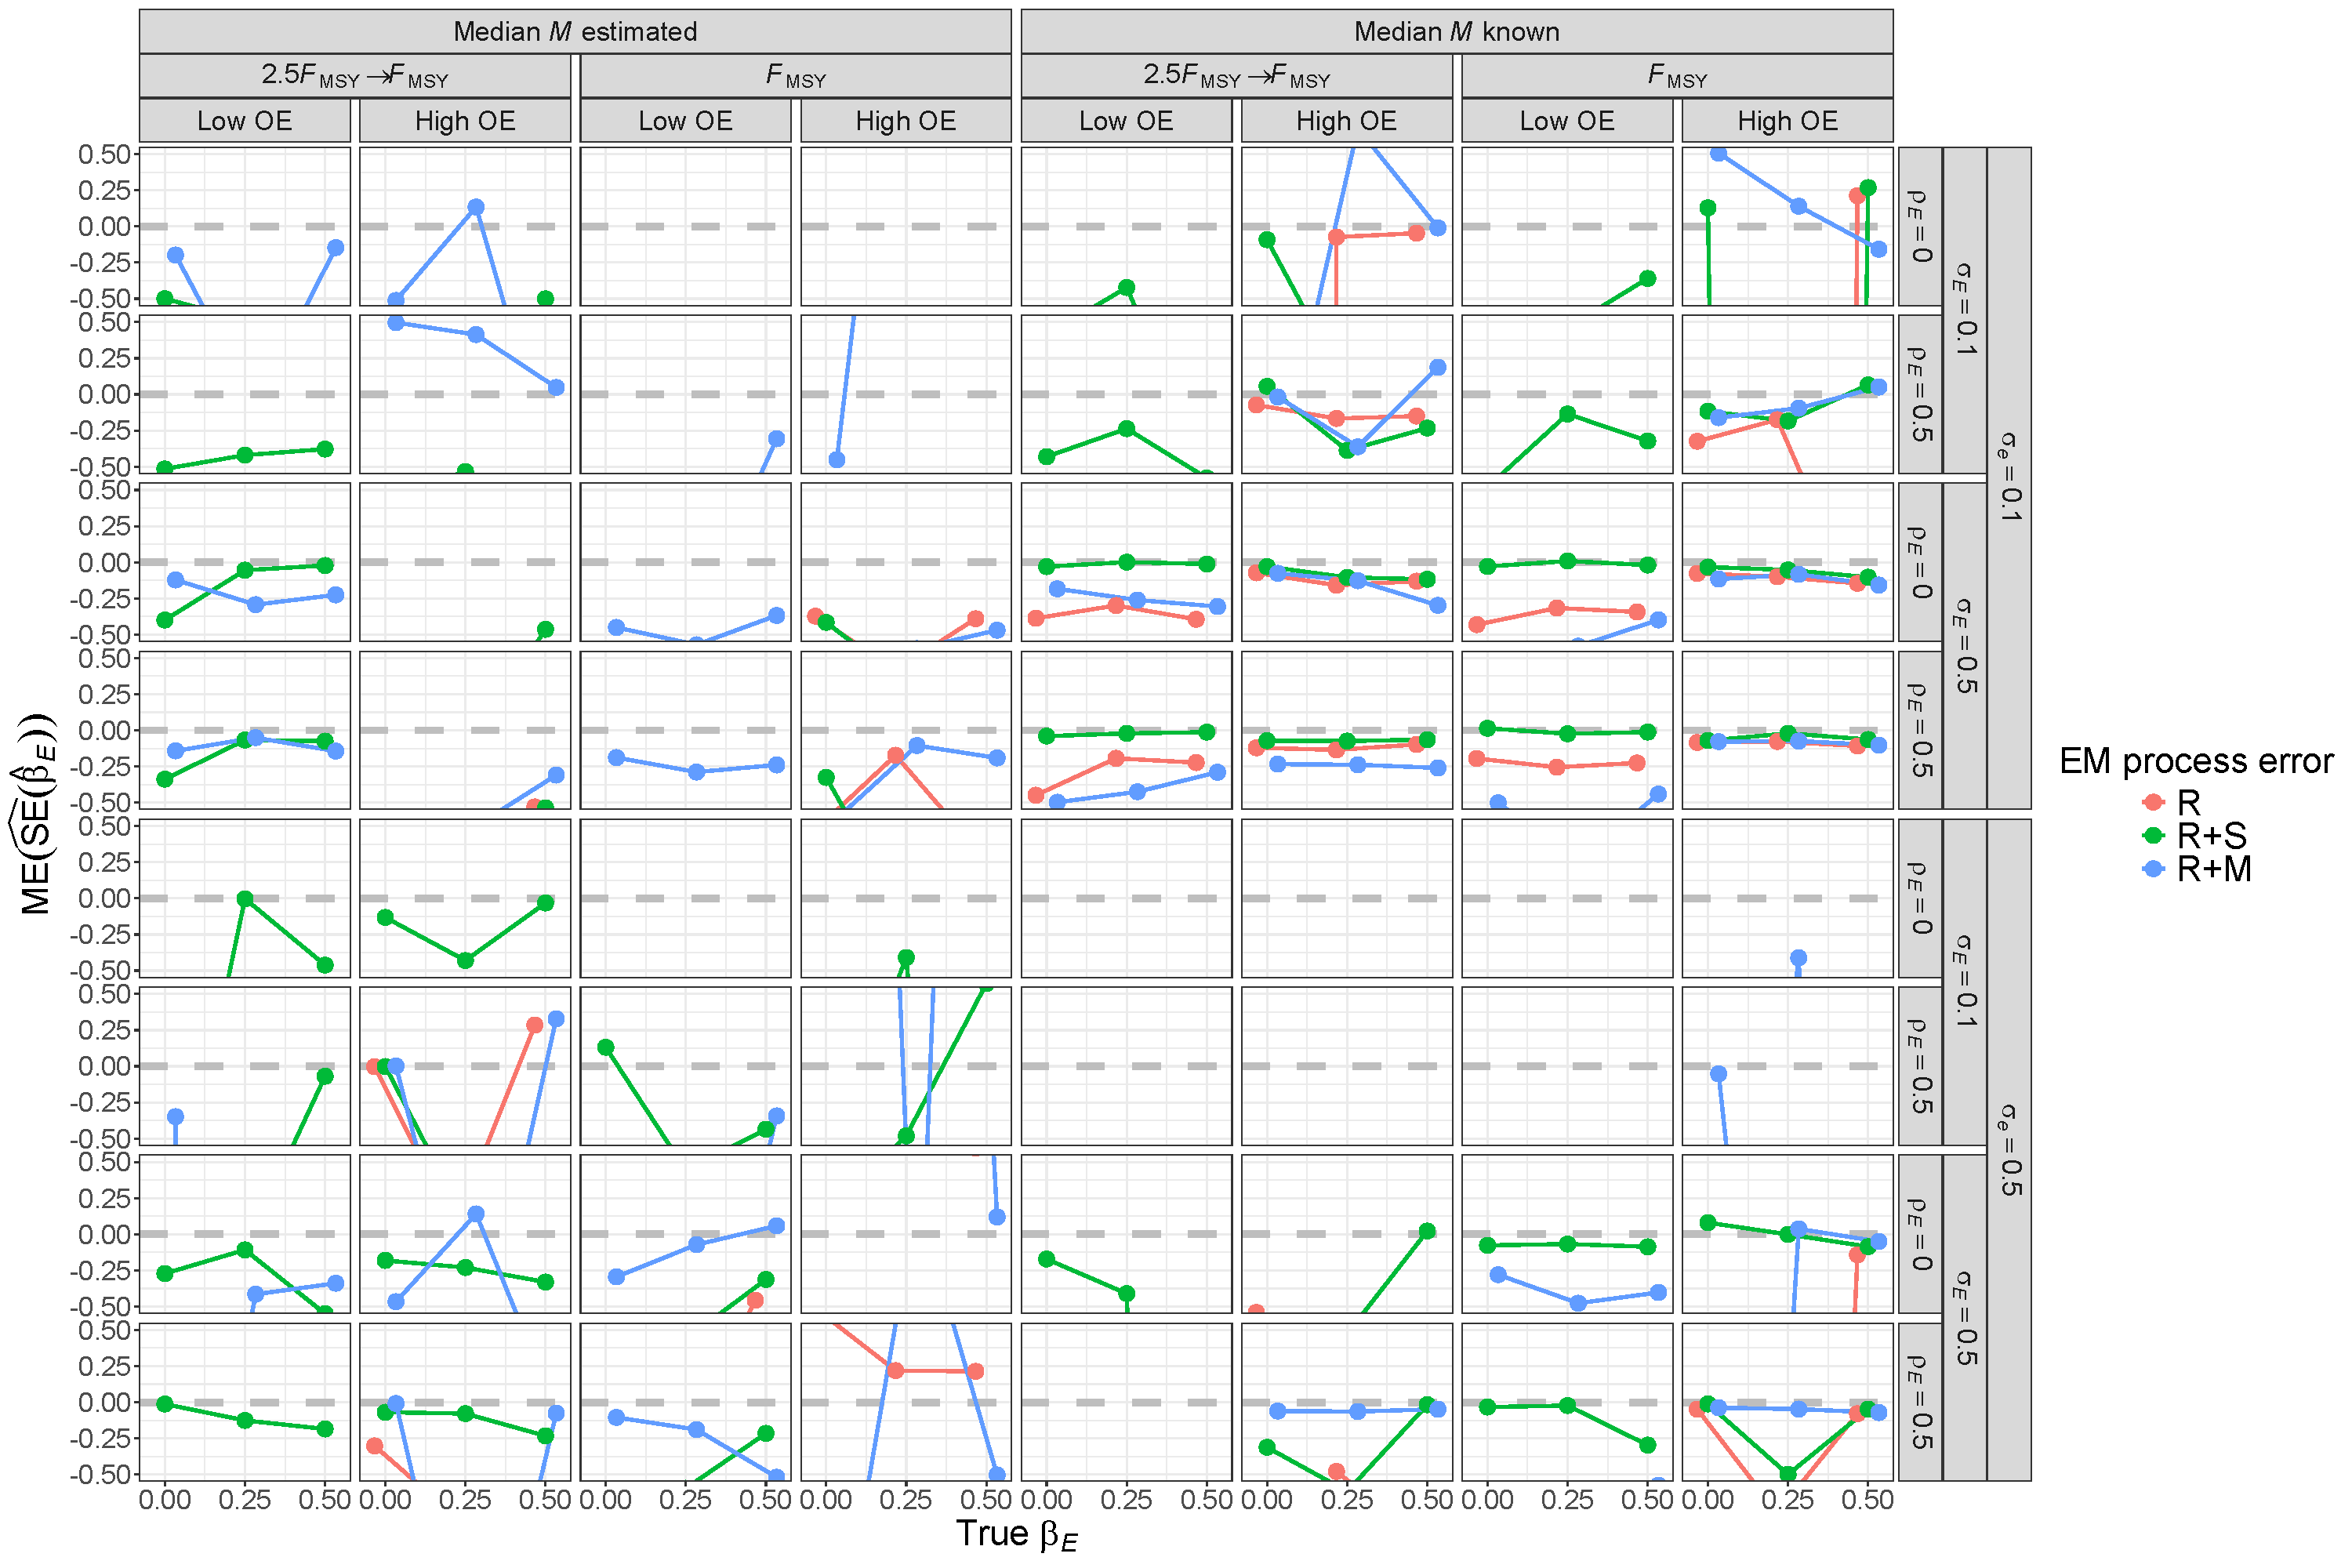
\includegraphics[height = \textheight]{se_beta_E_bias_RSom}
%DIFDELCMD < \end{center}
%DIFDELCMD < %%%
%DIFDELCMD < \caption{%
{%DIFAUXCMD
\DIFdelFL{For R+S OMs, median error (ME) of Hessian-based estimates of standard error for covariate effect on $M$ ($\beta_E$) from fitting EMs with alternative process error assumptions and treatment of median $M$ parameter ($\beta_M$). True standard error is defined as the mean of the standard error estimates accross converged fits to simulated data sets for a given OM scenario.}}%DIFAUXCMD
%DIFDELCMD < \label{se_beta_E_bias_RSom}
%DIFDELCMD < \end{figure}
%DIFDELCMD < \end{landscape}
%DIFDELCMD < 

%DIFDELCMD < \begin{landscape}
%DIFDELCMD < \begin{figure}
%DIFDELCMD < \begin{center}
%DIFDELCMD < 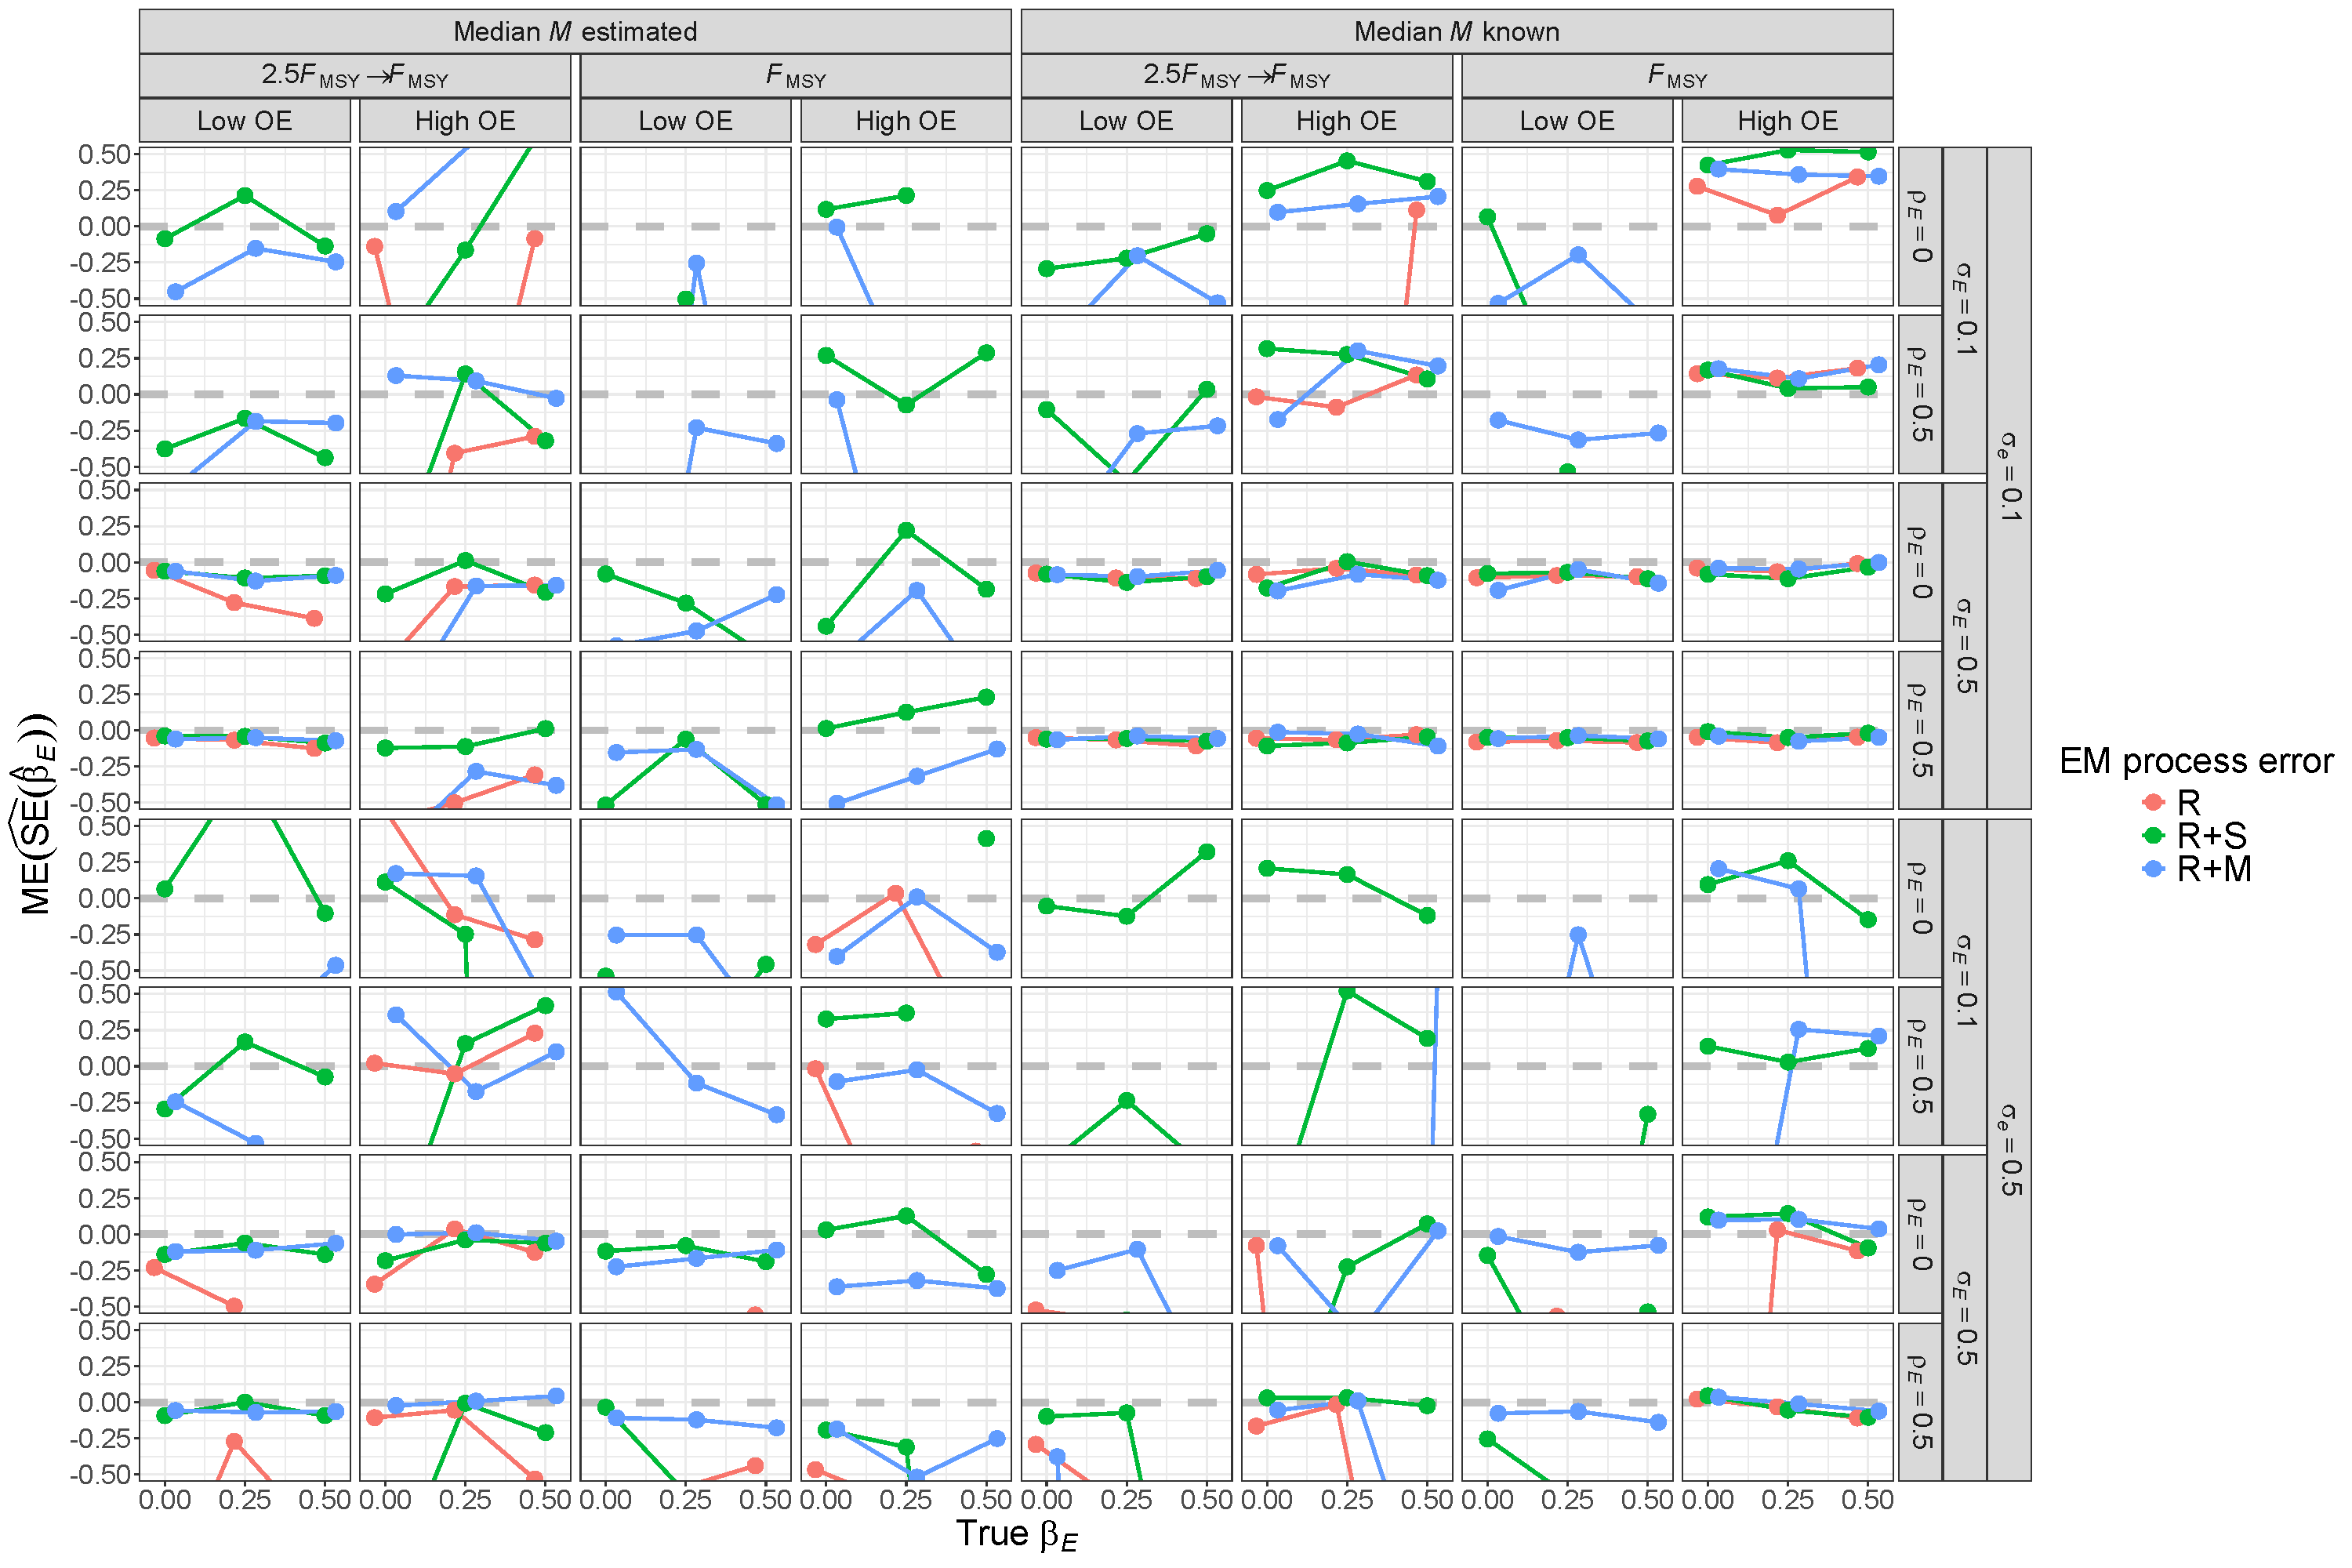
\includegraphics[height = \textheight]{se_beta_E_bias_RMom}
%DIFDELCMD < \end{center}
%DIFDELCMD < %%%
%DIFDELCMD < \caption{%
{%DIFAUXCMD
\DIFdelFL{For R+M OMs, median error (ME) of Hessian-based estimates of standard error for covariate effect on $M$ ($\beta_E$) from fitting EMs with alternative process error assumptions and treatment of median $M$ parameter ($\beta_M$). True standard error is defined as the mean of the standard error estimates accross converged fits to simulated data sets for a given OM scenario.}}%DIFAUXCMD
%DIFDELCMD < \label{se_beta_E_bias_RMom}
%DIFDELCMD < \end{figure}
%DIFDELCMD < \end{landscape}
%DIFDELCMD < 

%DIFDELCMD < %%%
\subsection*{\DIFdel{Covariate effect confidence interval coverage}}%DIFAUXCMD
%DIFDELCMD < \label{covariate-effect-confidence-interval-coverage}
%DIFDELCMD < %%%
\addcontentsline{toc}{subsection}{\DIFdel{Covariate effect confidence interval coverage}}
%DIFAUXCMD
%DIFDELCMD < 

%DIFDELCMD < \begin{landscape}
%DIFDELCMD < \begin{figure}
%DIFDELCMD < \begin{center}
%DIFDELCMD < 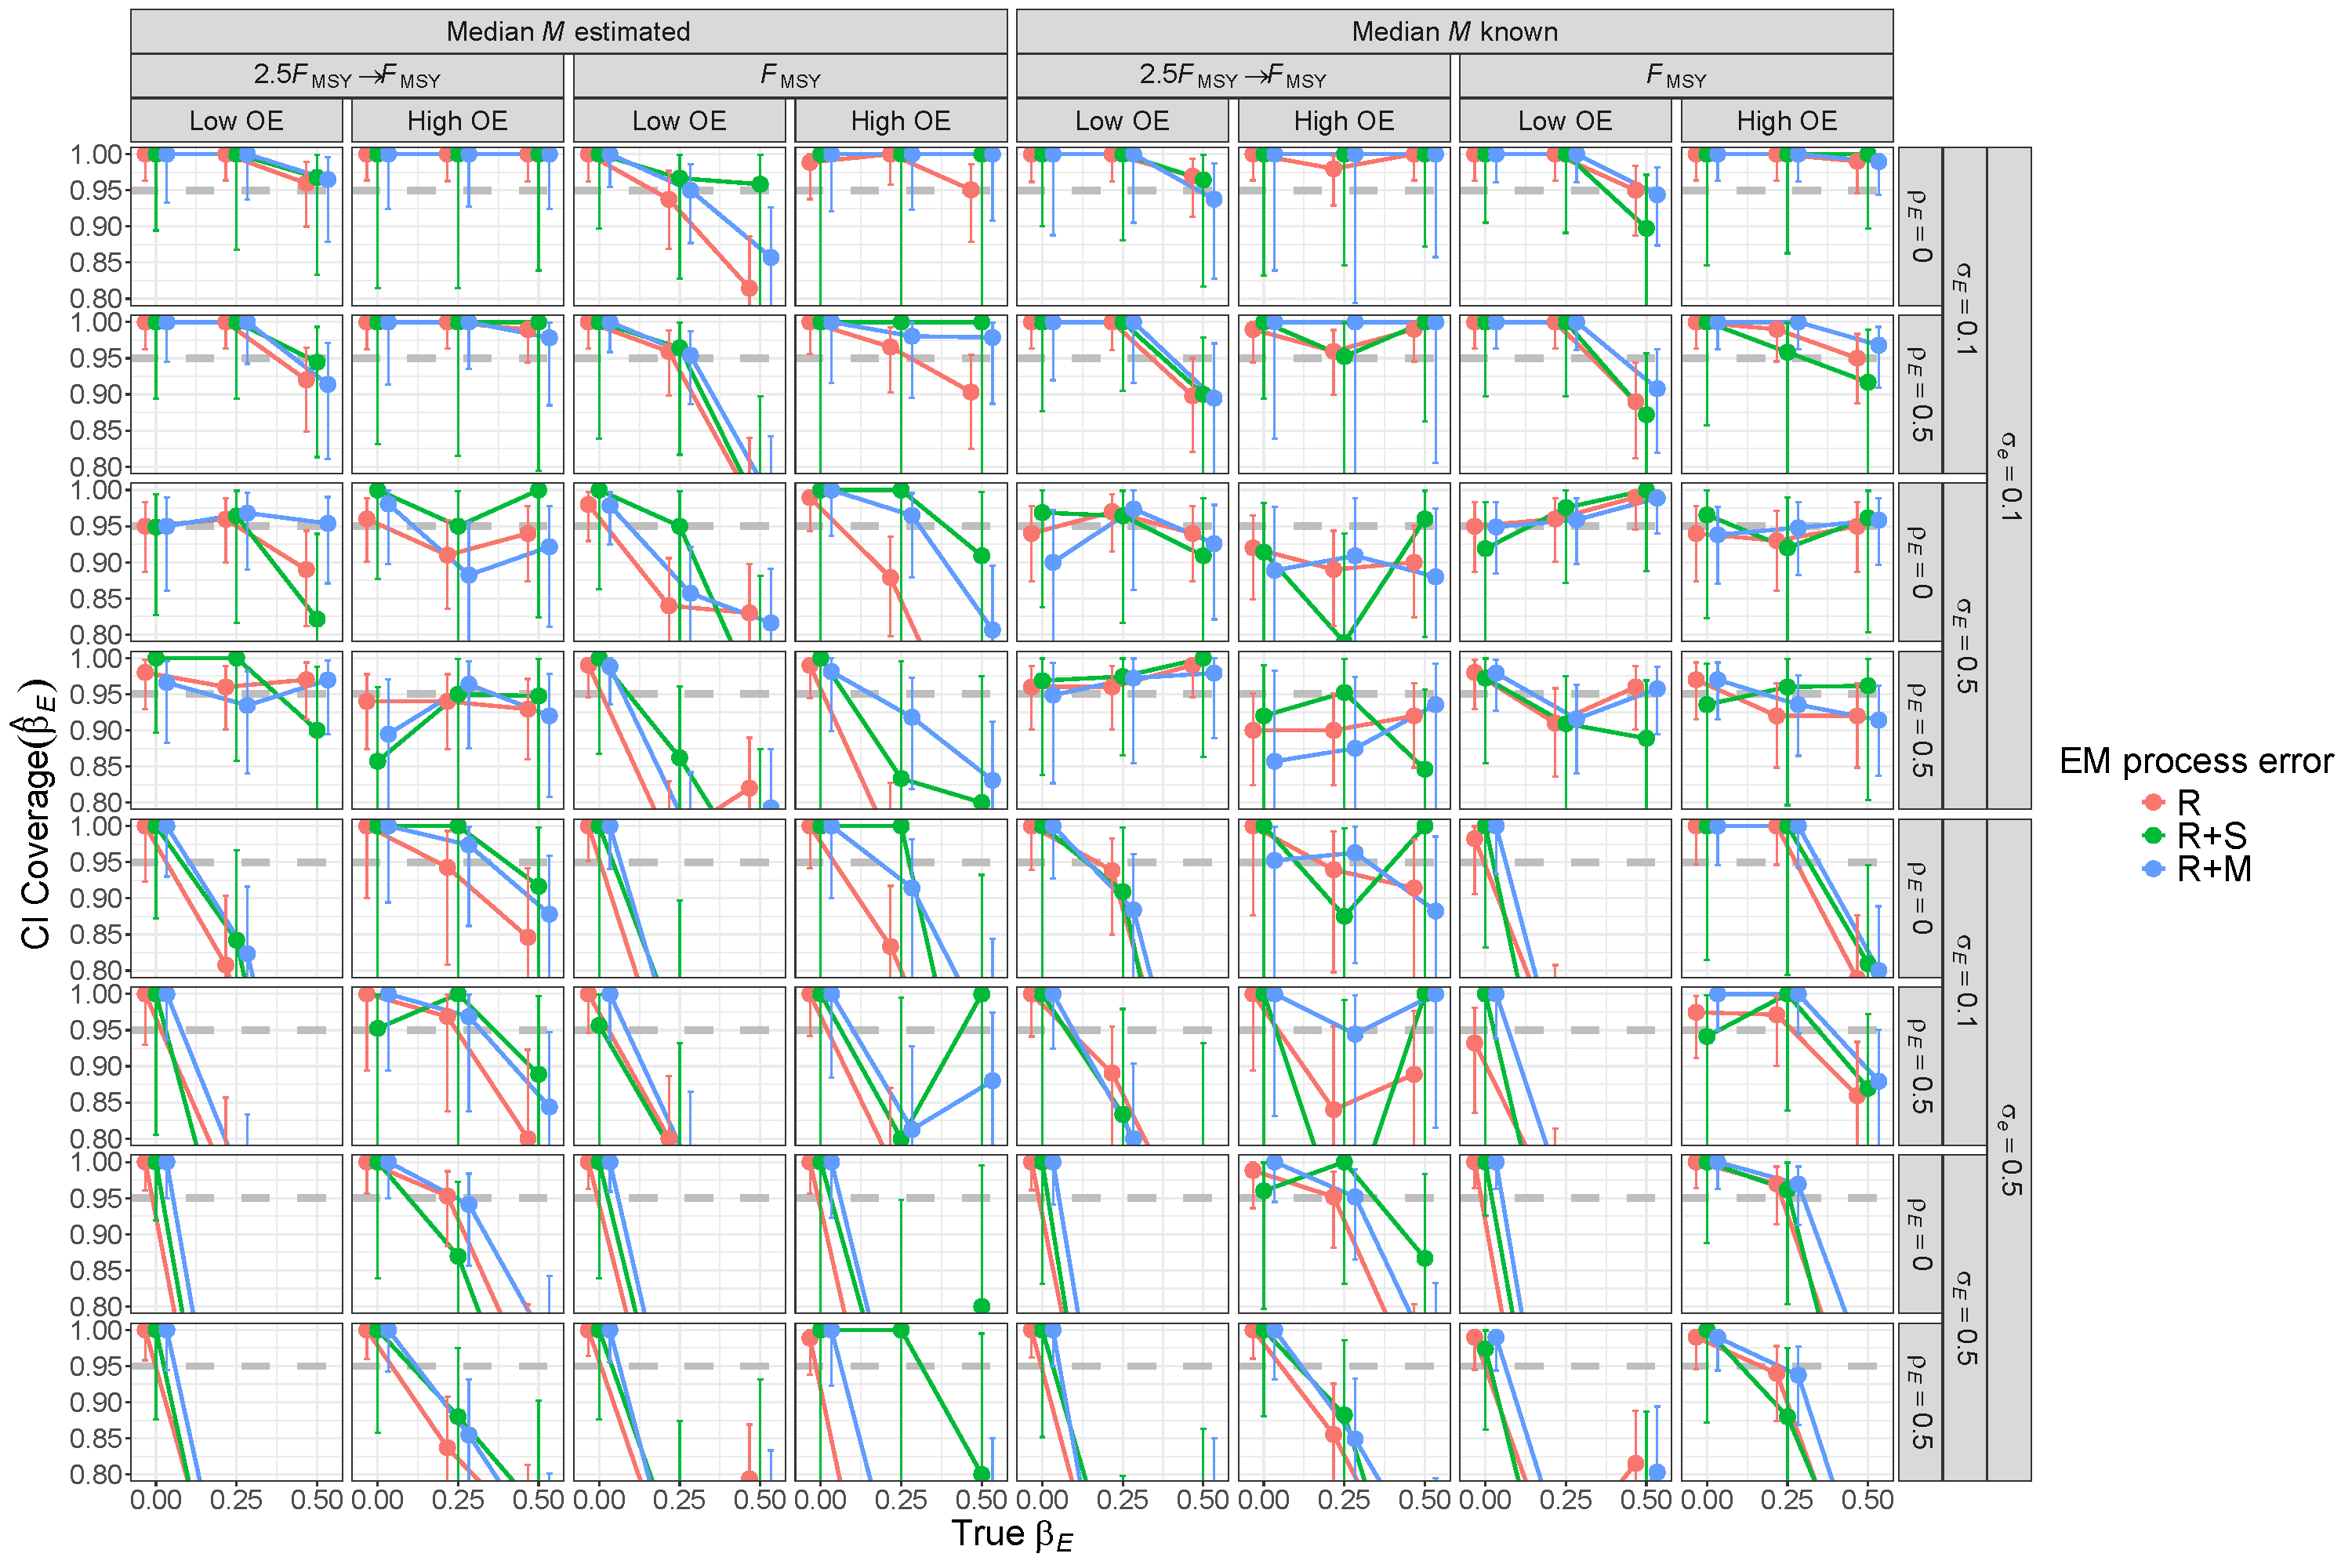
\includegraphics[height = \textheight]{beta_E_CI_coverage_Rom}
%DIFDELCMD < \end{center}
%DIFDELCMD < %%%
%DIFDELCMD < \caption{%
{%DIFAUXCMD
\DIFdelFL{For R OMs, probability of 95\% confidence interval for $\beta_E$ containing the true value for EMs with alternative process error assumptions and treatment of median $M$ parameter ($\beta_M$). Vertical lines represent 95\% confidence intervals.}}%DIFAUXCMD
%DIFDELCMD < \label{beta_E_CI_coverage_Rom}
%DIFDELCMD < \end{figure}
%DIFDELCMD < \end{landscape}
%DIFDELCMD < 

%DIFDELCMD < \begin{landscape}
%DIFDELCMD < \begin{figure}
%DIFDELCMD < \begin{center}
%DIFDELCMD < 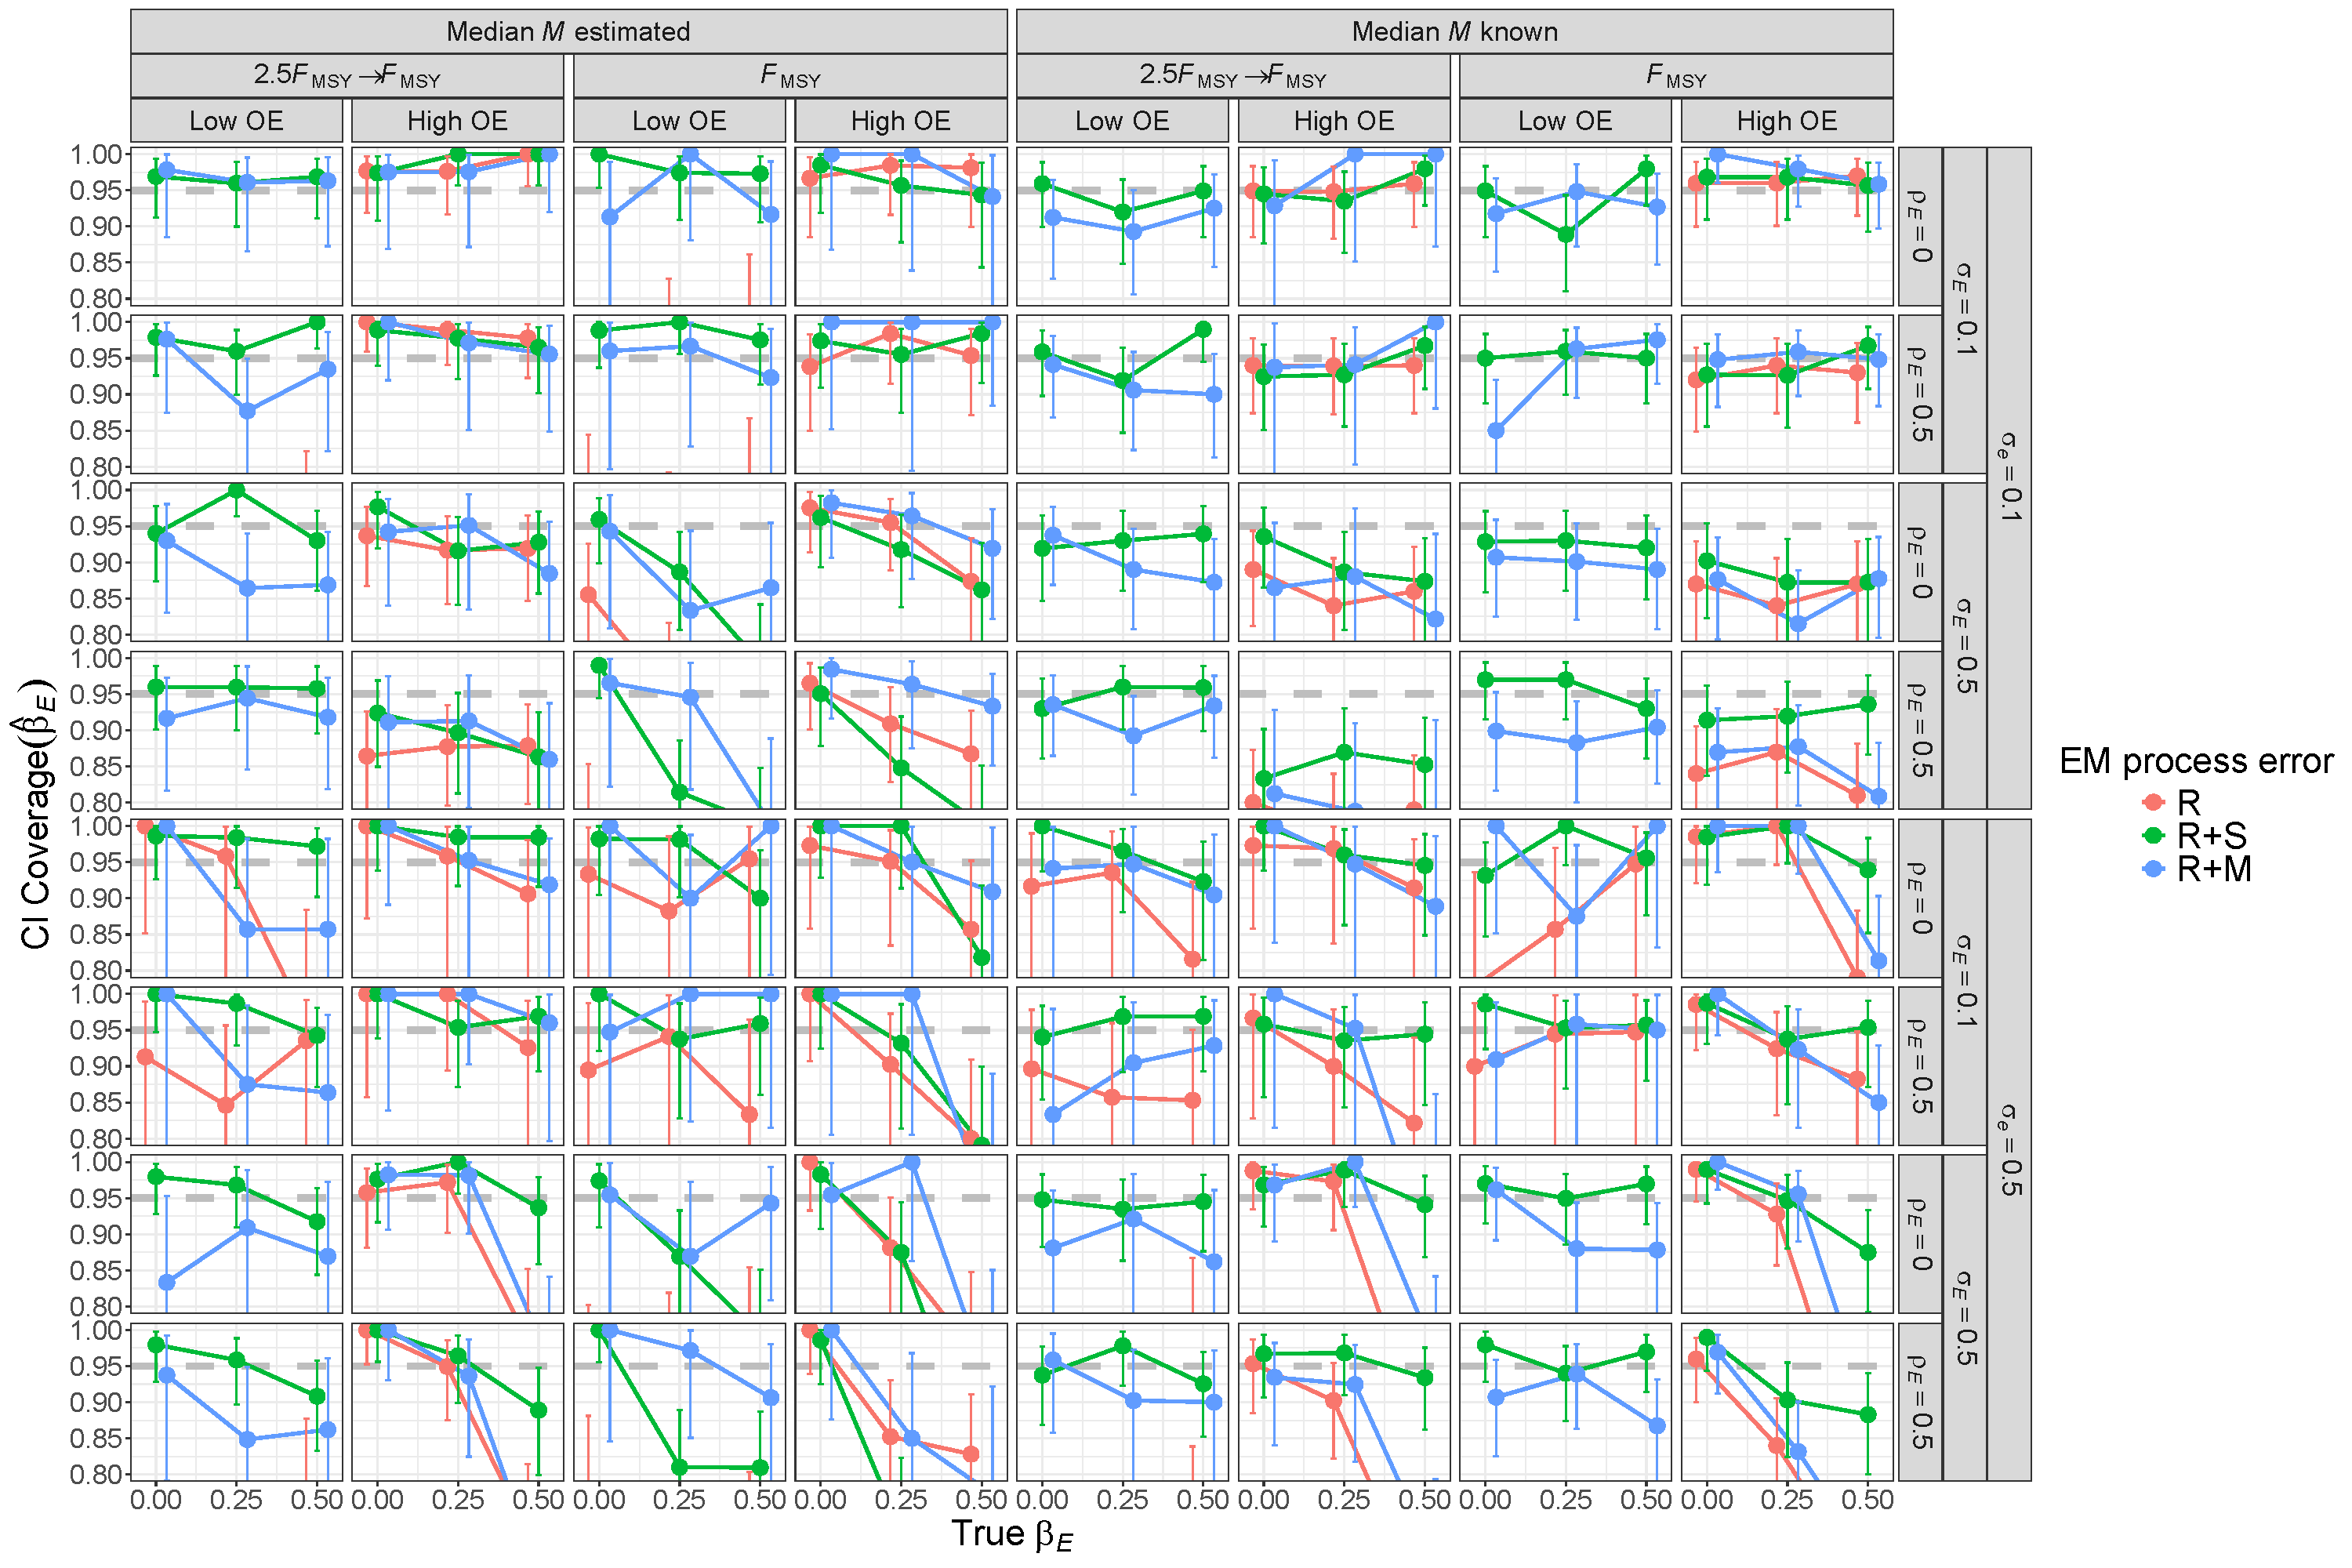
\includegraphics[height = \textheight]{beta_E_CI_coverage_RSom}
%DIFDELCMD < \end{center}
%DIFDELCMD < %%%
%DIFDELCMD < \caption{%
{%DIFAUXCMD
\DIFdelFL{For R+S OMs, probability of 95\% confidence interval for $\beta_E$ containing the true value for EMs with alternative process error assumptions and treatment of median $M$ parameter ($\beta_M$). Vertical lines represent 95\% confidence intervals.}}%DIFAUXCMD
%DIFDELCMD < \label{beta_E_CI_coverage_RSom}
%DIFDELCMD < \end{figure}
%DIFDELCMD < \end{landscape}
%DIFDELCMD < 

%DIFDELCMD < \begin{landscape}
%DIFDELCMD < \begin{figure}
%DIFDELCMD < \begin{center}
%DIFDELCMD < 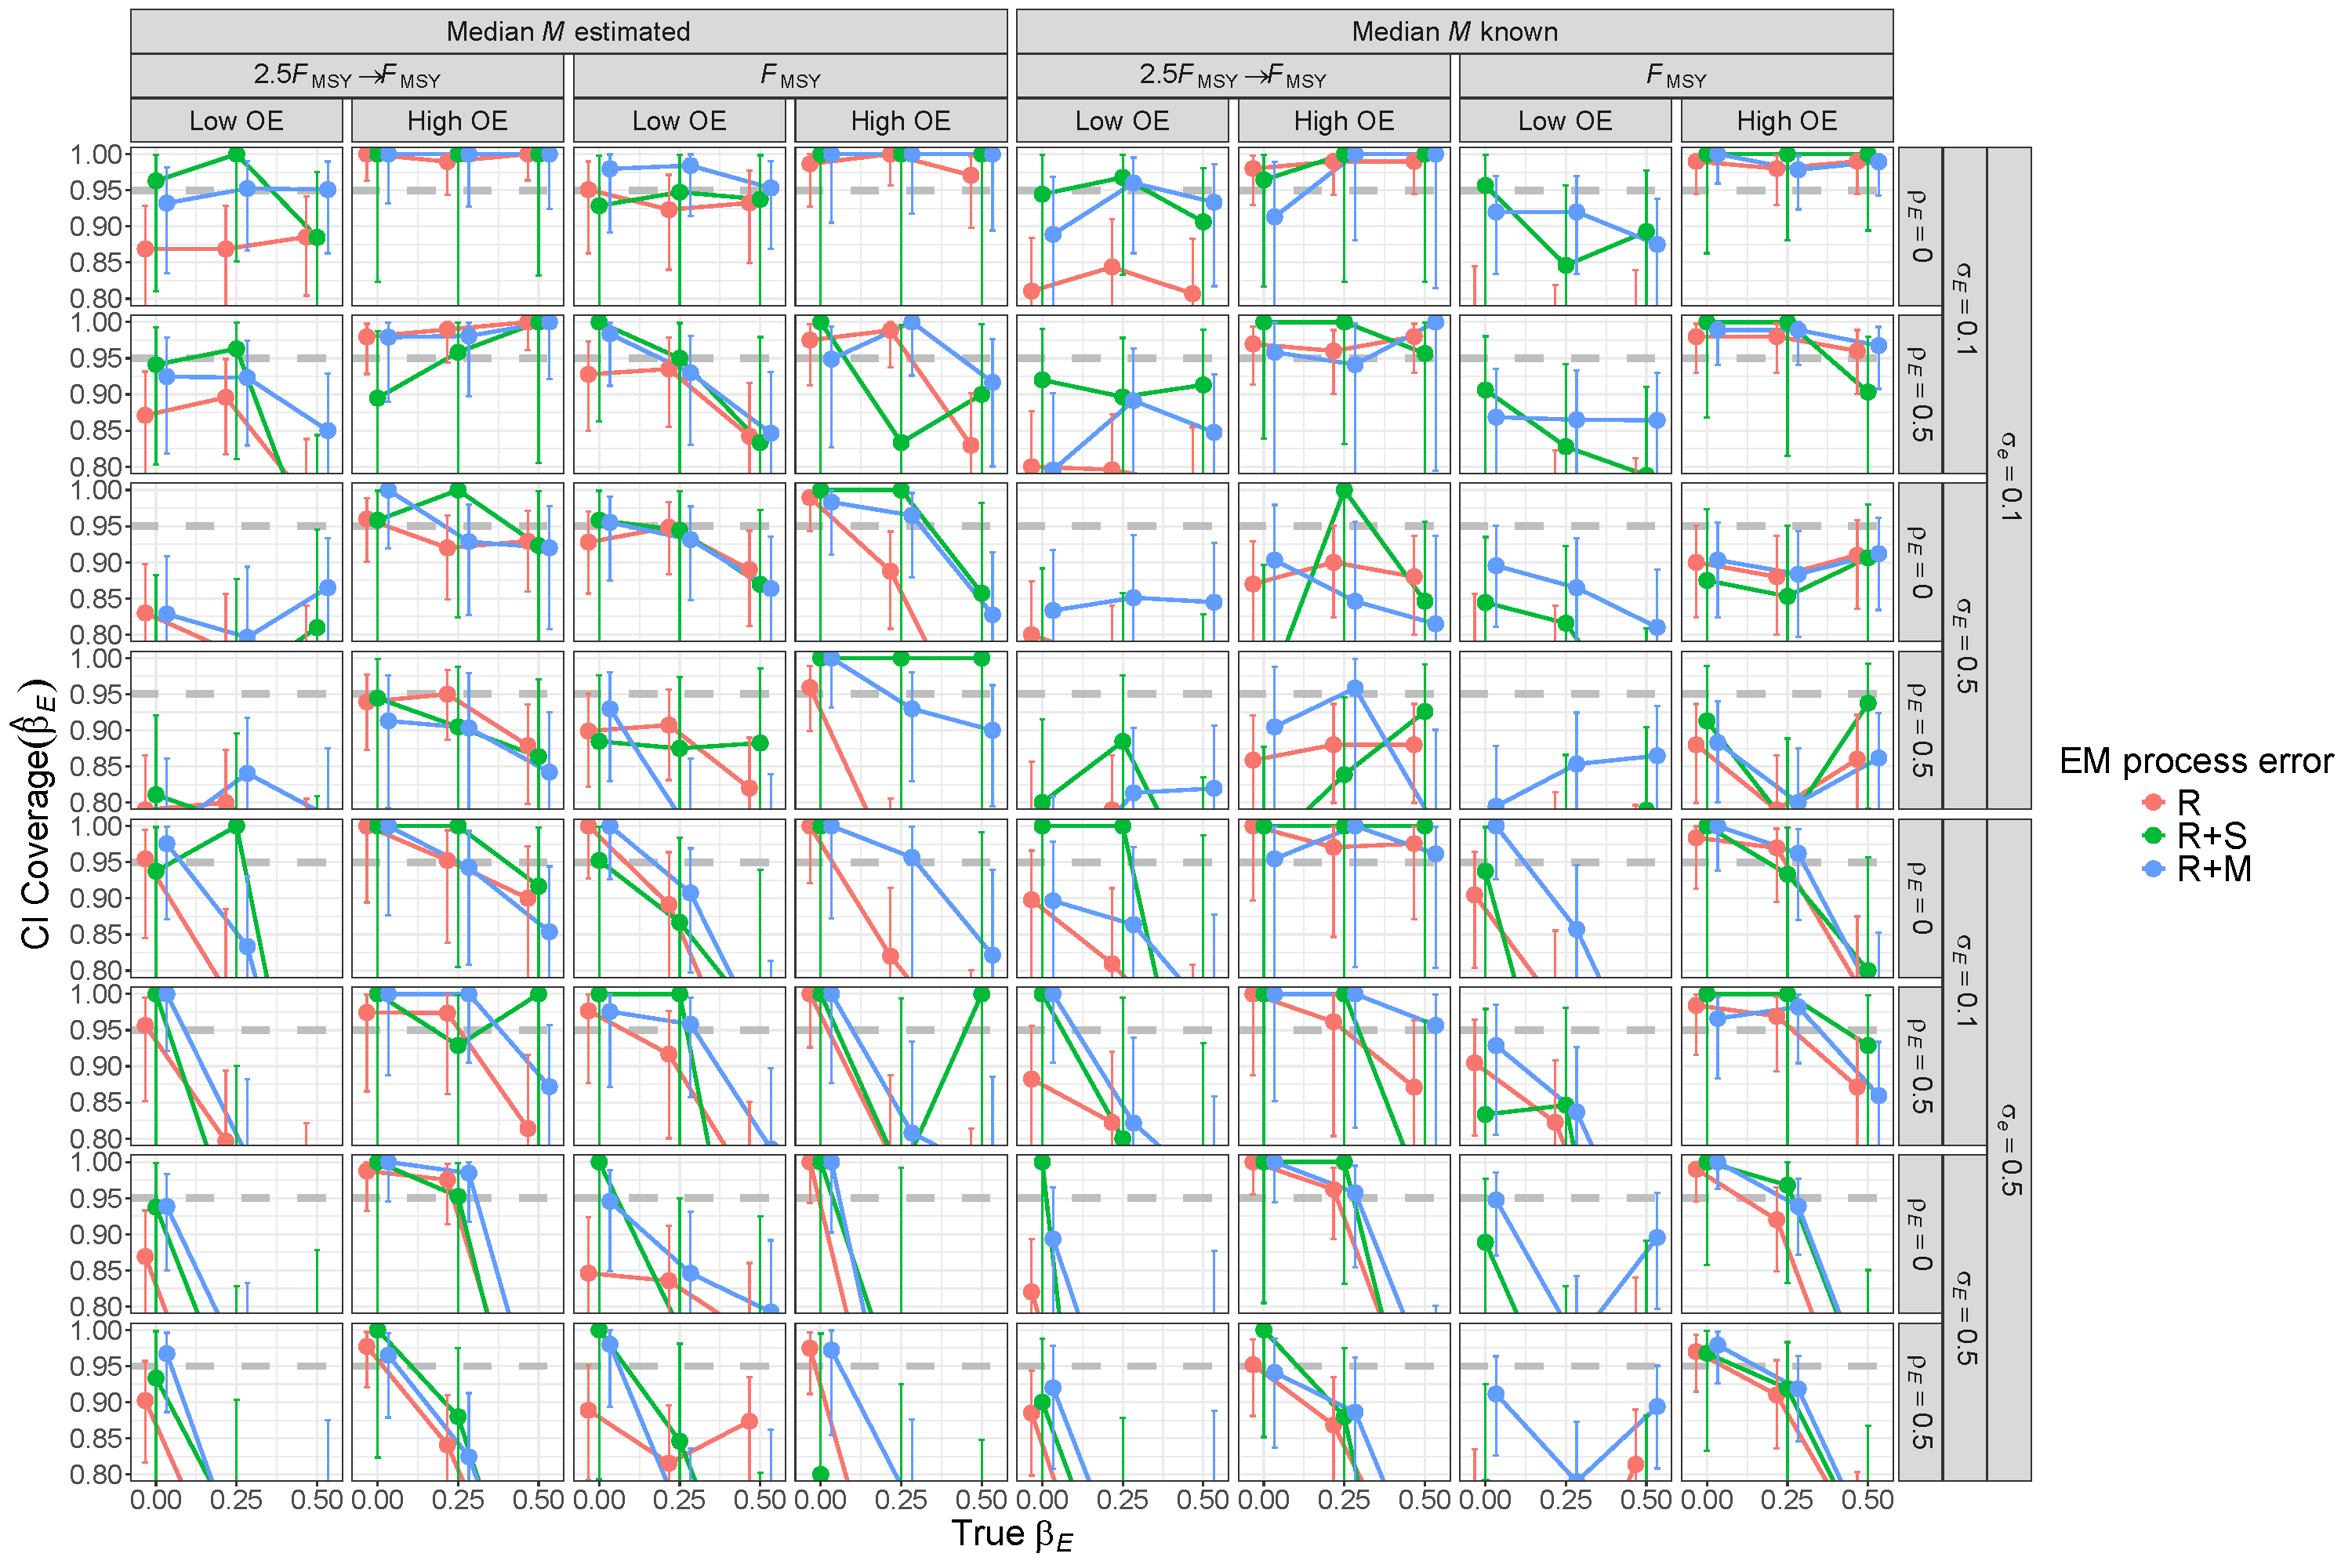
\includegraphics[height = \textheight]{beta_E_CI_coverage_RMom}
%DIFDELCMD < \end{center}
%DIFDELCMD < %%%
%DIFDELCMD < \caption{%
{%DIFAUXCMD
\DIFdelFL{For R+M OMs, probability of 95\% confidence interval for $\beta_E$ containing the true value for EMs with alternative process error assumptions and treatment of median $M$ parameter ($\beta_M$). Vertical lines represent 95\% confidence intervals.}}%DIFAUXCMD
%DIFDELCMD < \label{beta_E_CI_coverage_RMom}
%DIFDELCMD < \end{figure}
%DIFDELCMD < \end{landscape}
%DIFDELCMD < 

%DIFDELCMD < %%%
\subsection*{\DIFdel{Covariate effect RMSE}}%DIFAUXCMD
%DIFDELCMD < \label{covariate-effect-rmse}
%DIFDELCMD < %%%
\addcontentsline{toc}{subsection}{\DIFdel{Covariate effect RMSE}}
%DIFAUXCMD
%DIFDELCMD < 

%DIFDELCMD < \begin{landscape}
%DIFDELCMD < \begin{figure}
%DIFDELCMD < \begin{center}
%DIFDELCMD < 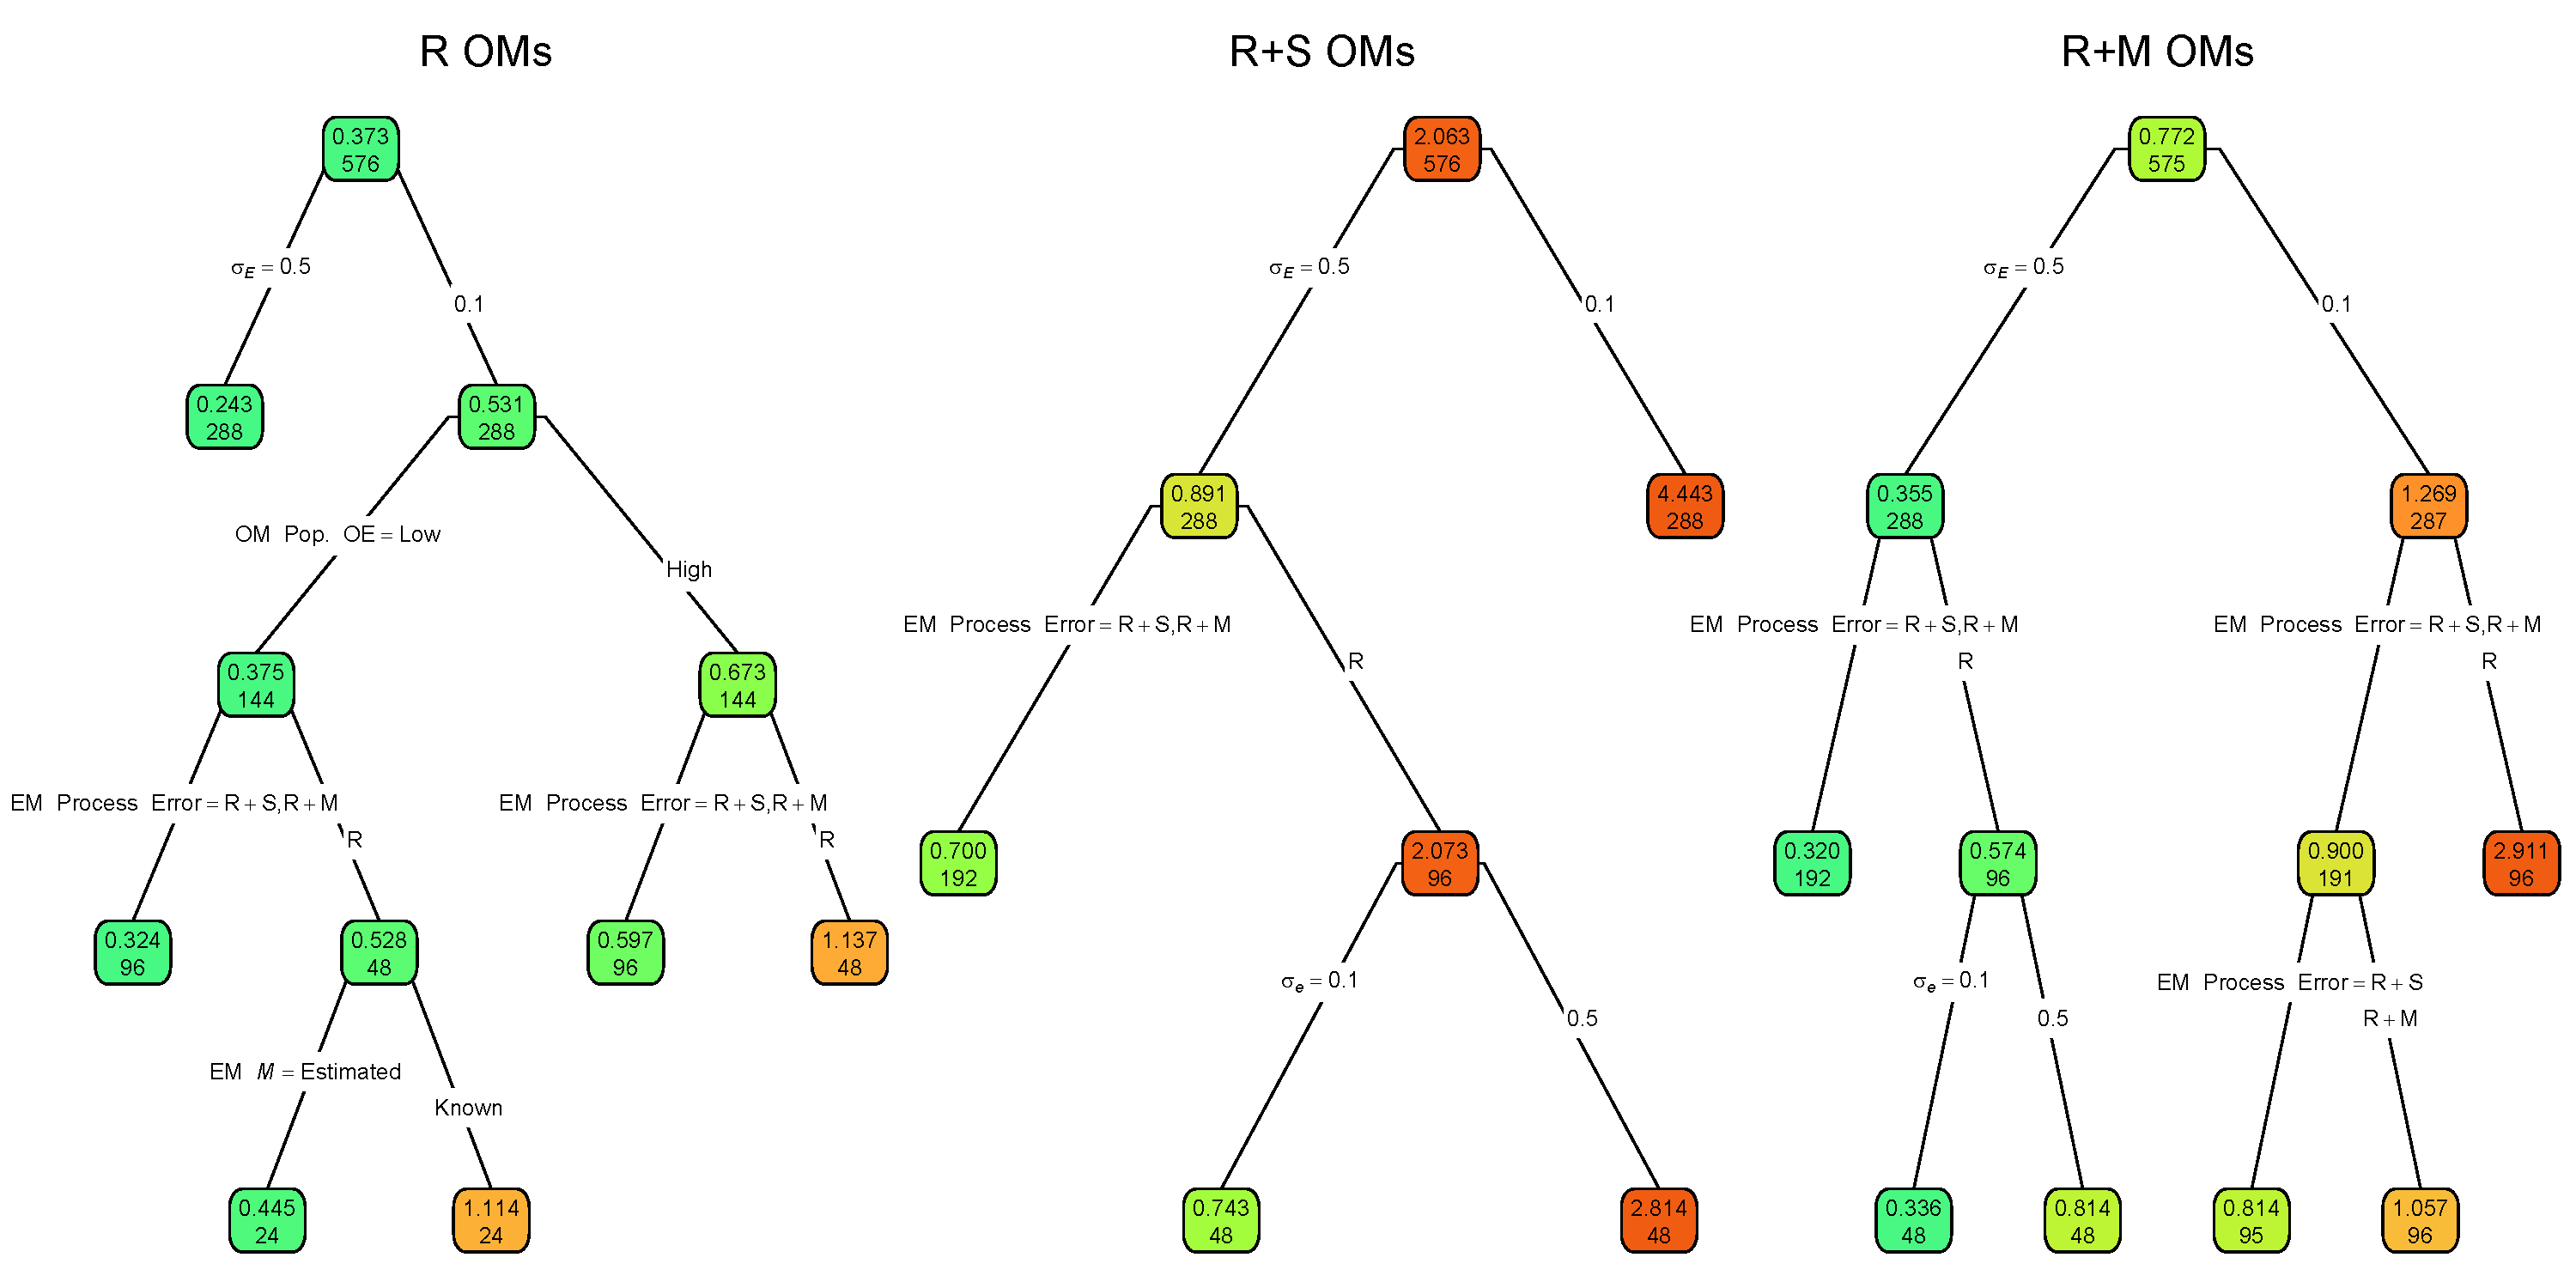
\includegraphics[width = 1.4\textwidth]{ecov_beta_rmse_regtree_plots}
%DIFDELCMD < \end{center}
%DIFDELCMD < %%%
%DIFDELCMD < \caption{%
{%DIFAUXCMD
\DIFdelFL{Regression trees indicating primary factors determining reductions in sums of squares for the log-transformed RMSE of covariate effect on $M$ ($\text{RMSE}\left(\widehat \beta_E\right)$) for operating models (OMs) with process error on recruitment only (R), recruitment and apparent survival (R+S), or recruitment and natural mortality (R+M). Each node shows the median error (top) and number of observations (bottom) for the corresponding subset. Lower or higher median RMSE are indicated by more green or red polygons, respectively.}}%DIFAUXCMD
%DIFDELCMD < \label{ecov_effect_rmse_regtree}
%DIFDELCMD < \end{figure}
%DIFDELCMD < \end{landscape}
%DIFDELCMD < 

%DIFDELCMD < %%%
\DIFdelend \begin{table}
\caption{Percent reduction in deviance \DIFdelbeginFL \DIFdelFL{forlinear }\DIFdelendFL \DIFaddbeginFL \DIFaddFL{for linear }\DIFaddendFL regression models fit to \DIFdelbeginFL \DIFdelFL{the }\DIFdelendFL log-transformed RMSE \DIFdelbeginFL \DIFdelFL{for estimates }\DIFdelendFL of \DIFdelbeginFL \DIFdelFL{the covariate effect on $M$  }\DIFdelendFL \DIFaddbeginFL \DIFaddFL{terminal year spawning stock biomass }\DIFaddendFL (\DIFdelbeginFL \DIFdelFL{$\text{RMSE}\left(\widehat \beta_E\right)$}\DIFdelendFL \DIFaddbeginFL \DIFaddFL{SSB}\DIFaddendFL ). \DIFdelbeginFL \DIFdelFL{Table rows give each operating model (OM) }\DIFdelendFL \DIFaddbeginFL \DIFaddFL{See Tables \ref{convergence_PRD_table} }\DIFaddendFL and \DIFdelbeginFL \DIFdelFL{estimating model (EM) factor included individually, combined, and with second and third order interactions}\DIFdelendFL \DIFaddbeginFL \DIFaddFL{\ref{factor_table} for further details}\DIFaddendFL .\DIFdelbeginFL \DIFdelFL{Table columns are operating models (OMs) with process error on recruitment only (R), recruitment and apparent survival (R+S), or recruitment and natural mortality (R+M).}\DIFdelendFL }\DIFdelbeginFL %DIFDELCMD < \label{RMSE_ecov_beta_PRD_table}
%DIFDELCMD < %%%
\DIFdelendFL \DIFaddbeginFL \label{rmse_SSB_PRD_table}
\DIFaddendFL {\begin{center}
\begin{tabular}{lrrr}
\hline\hline
\multicolumn{1}{l}{Factor}&\multicolumn{1}{c}{R}&\multicolumn{1}{c}{R+S}&\multicolumn{1}{c}{R+M}\tabularnewline
\hline
OM $F$ history&\DIFdelbeginFL \DIFdelFL{0.50}\DIFdelendFL \DIFaddbeginFL \DIFaddFL{19.88}\DIFaddendFL &\DIFdelbeginFL \DIFdelFL{0.11}\DIFdelendFL \DIFaddbeginFL \DIFaddFL{32.67}\DIFaddendFL &\DIFdelbeginFL \DIFdelFL{0.12}\DIFdelendFL \DIFaddbeginFL \DIFaddFL{20.92}\DIFaddendFL \tabularnewline
OM Obs. Error& \DIFdelbeginFL \DIFdelFL{12.04}\DIFdelendFL \DIFaddbeginFL \DIFaddFL{2.21}\DIFaddendFL & \DIFdelbeginFL \DIFdelFL{5.66}\DIFdelendFL \DIFaddbeginFL \DIFaddFL{0.11}\DIFaddendFL & \DIFdelbeginFL \DIFdelFL{0.36}\DIFdelendFL \DIFaddbeginFL \DIFaddFL{1.48}\DIFaddendFL \tabularnewline
\DIFdelbeginFL \DIFdelFL{$OM \sigma_e$}\DIFdelendFL \DIFaddbeginFL \DIFaddFL{OM $\sigma_e$}\DIFaddendFL & \DIFdelbeginFL \DIFdelFL{0.87}\DIFdelendFL \DIFaddbeginFL \DIFaddFL{0.05}\DIFaddendFL & \DIFdelbeginFL \DIFdelFL{5.78}\DIFdelendFL \DIFaddbeginFL \DIFaddFL{0.16}\DIFaddendFL & \DIFdelbeginFL \DIFdelFL{2.60}\DIFdelendFL \DIFaddbeginFL \DIFaddFL{0.03}\DIFaddendFL \tabularnewline
\DIFdelbeginFL \DIFdelFL{$OM \sigma_E$}\DIFdelendFL \DIFaddbeginFL \DIFaddFL{OM $\sigma_E$}\DIFaddendFL & \DIFdelbeginFL \DIFdelFL{15.85}\DIFdelendFL \DIFaddbeginFL \DIFaddFL{0.08}\DIFaddendFL & \DIFdelbeginFL \DIFdelFL{24.18}\DIFdelendFL \DIFaddbeginFL \DIFaddFL{0.16}\DIFaddendFL & \DIFdelbeginFL \DIFdelFL{24.26}\DIFdelendFL \DIFaddbeginFL \DIFaddFL{0.02}\DIFaddendFL \tabularnewline
\DIFdelbeginFL \DIFdelFL{$OM \rho_{E}$}\DIFdelendFL \DIFaddbeginFL \DIFaddFL{OM $\rho_{E}$}\DIFaddendFL & \DIFdelbeginFL \DIFdelFL{0.36}\DIFdelendFL \DIFaddbeginFL \DIFaddFL{0.03}\DIFaddendFL &\DIFdelbeginFL \DIFdelFL{0.82}\DIFdelendFL \DIFaddbeginFL \DIFaddFL{\textless  0.01}\DIFaddendFL & \DIFdelbeginFL \DIFdelFL{0.34}\DIFdelendFL \DIFaddbeginFL \DIFaddFL{0.02}\DIFaddendFL \tabularnewline
OM $\beta_{E}$& \DIFdelbeginFL \DIFdelFL{6.72}\DIFdelendFL \DIFaddbeginFL \DIFaddFL{0.05}\DIFaddendFL & \DIFdelbeginFL \DIFdelFL{0.07}\DIFdelendFL \DIFaddbeginFL \DIFaddFL{0.03}\DIFaddendFL & \DIFdelbeginFL \DIFdelFL{0.96}\DIFdelendFL \DIFaddbeginFL \DIFaddFL{0.14}\DIFaddendFL \tabularnewline
EM Process Error& \DIFdelbeginFL \DIFdelFL{6.49}\DIFdelendFL \DIFaddbeginFL \DIFaddFL{5.72}\DIFaddendFL & \DIFdelbeginFL \DIFdelFL{11.31}\DIFdelendFL \DIFaddbeginFL \DIFaddFL{0.13}\DIFaddendFL & \DIFdelbeginFL \DIFdelFL{11.98}\DIFdelendFL \DIFaddbeginFL \DIFaddFL{5.73}\DIFaddendFL \tabularnewline
\DIFaddbeginFL \DIFaddFL{$EM \beta_{E}$ assumption}& \DIFaddFL{0.03}& \DIFaddFL{0.79}& \DIFaddFL{0.05}\tabularnewline
\DIFaddendFL EM $M$ assumption&\DIFdelbeginFL \DIFdelFL{0.04}\DIFdelendFL \DIFaddbeginFL \DIFaddFL{20.05}\DIFaddendFL &\DIFdelbeginFL \DIFdelFL{0.64}\DIFdelendFL \DIFaddbeginFL \DIFaddFL{21.11}\DIFaddendFL &\DIFdelbeginFL \DIFdelFL{0.07}\DIFdelendFL \DIFaddbeginFL \DIFaddFL{19.43}\DIFaddendFL \tabularnewline
All factors&\DIFdelbeginFL \DIFdelFL{42.87}\DIFdelendFL \DIFaddbeginFL \DIFaddFL{48.09}\DIFaddendFL &\DIFdelbeginFL \DIFdelFL{48.58}\DIFdelendFL \DIFaddbeginFL \DIFaddFL{55.17}\DIFaddendFL &\DIFdelbeginFL \DIFdelFL{40.65}\DIFdelendFL \DIFaddbeginFL \DIFaddFL{47.82}\DIFaddendFL \tabularnewline
+ All Two Way&\DIFdelbeginFL \DIFdelFL{67.34}\DIFdelendFL \DIFaddbeginFL \DIFaddFL{79.09}\DIFaddendFL &\DIFdelbeginFL \DIFdelFL{74.09}\DIFdelendFL \DIFaddbeginFL \DIFaddFL{80.98}\DIFaddendFL &\DIFdelbeginFL \DIFdelFL{61.74}\DIFdelendFL \DIFaddbeginFL \DIFaddFL{78.40}\DIFaddendFL \tabularnewline
+ All Three Way&\DIFdelbeginFL \DIFdelFL{79.42}\DIFdelendFL \DIFaddbeginFL \DIFaddFL{88.30}\DIFaddendFL &\DIFdelbeginFL \DIFdelFL{82.75}\DIFdelendFL \DIFaddbeginFL \DIFaddFL{89.49}\DIFaddendFL &\DIFdelbeginFL \DIFdelFL{71.92}\DIFdelendFL \DIFaddbeginFL \DIFaddFL{87.67}\DIFaddendFL \tabularnewline
\hline
\end{tabular}\end{center}
}
\end{table}
\DIFaddbegin \pagebreak
\DIFaddend 

\DIFdelbegin %DIFDELCMD < \begin{landscape}
%DIFDELCMD < \begin{figure}
%DIFDELCMD < \begin{center}
%DIFDELCMD < 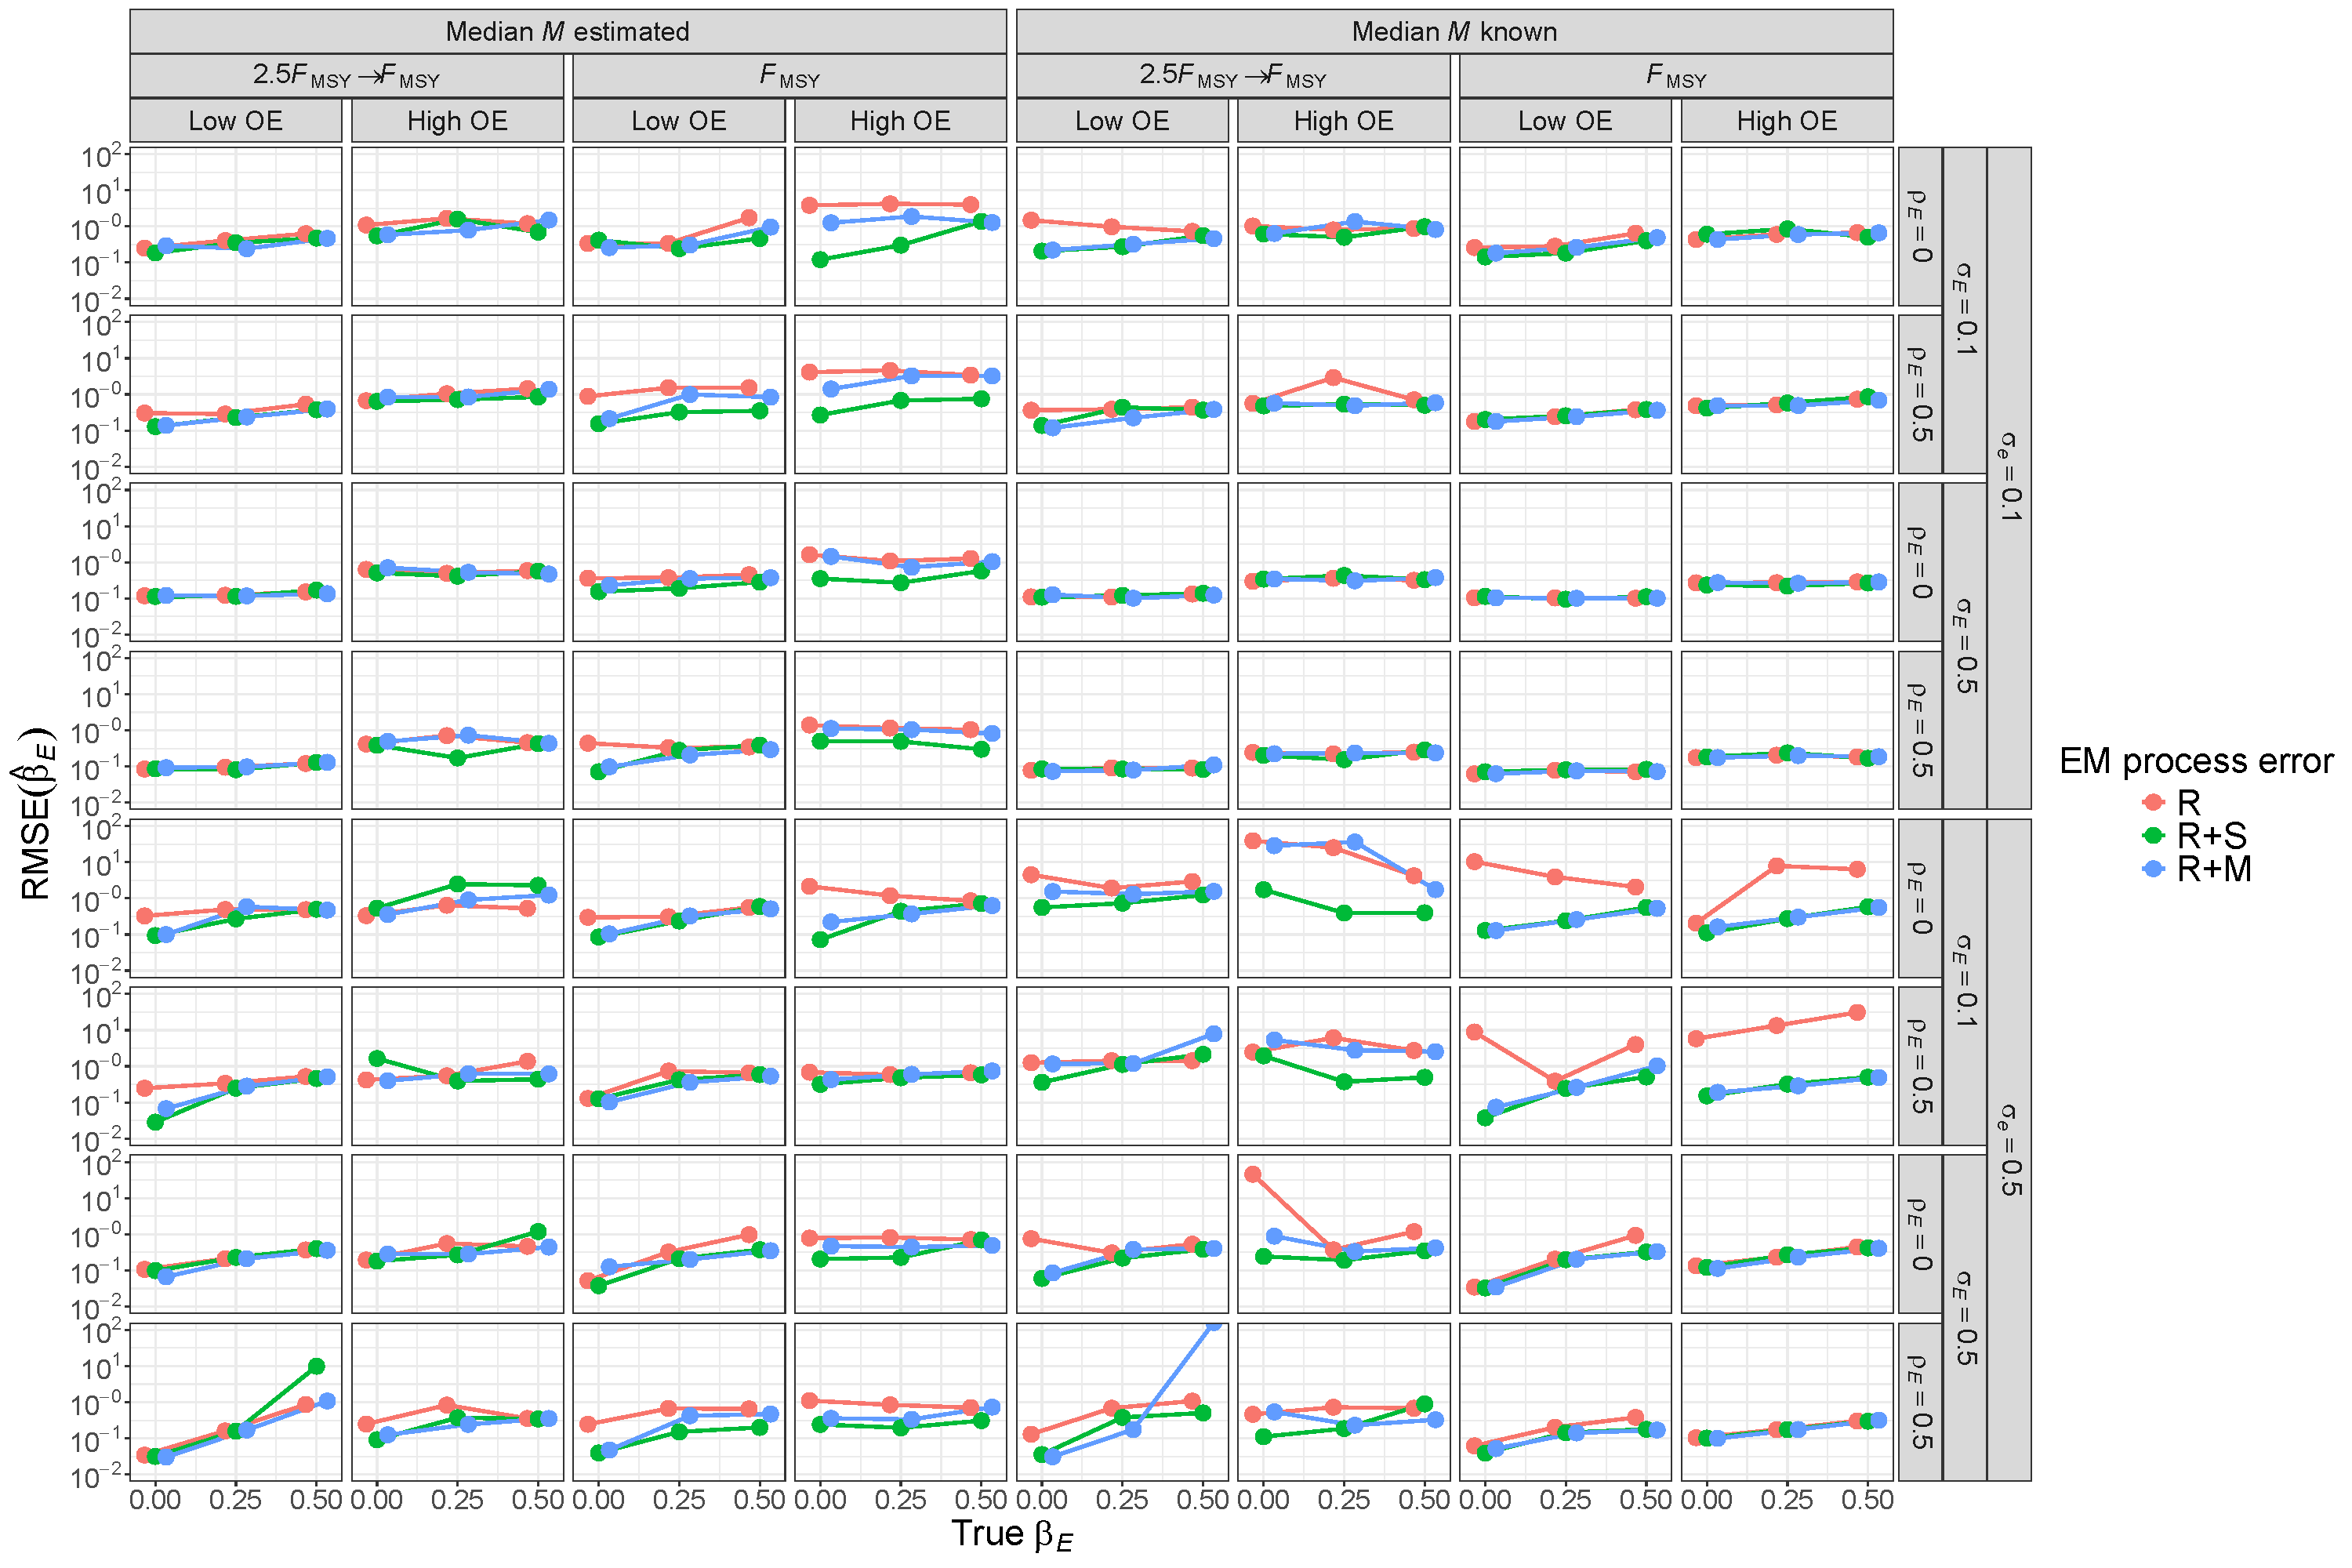
\includegraphics[height = \textheight]{beta_E_rmse_Rom}
%DIFDELCMD < \end{center}
%DIFDELCMD < %%%
%DIFDELCMD < \caption{%
{%DIFAUXCMD
\DIFdelFL{For R OMs, RMSE of estimates of covariate effect on $M$ ($\beta_E$) from fitting EMs with alternative process error assumptions and treatment of median $M$ parameter ($\beta_M$). }}%DIFAUXCMD
%DIFDELCMD < \label{beta_E_rmse_Rom}
%DIFDELCMD < \end{figure}
%DIFDELCMD < \end{landscape}
%DIFDELCMD < 

%DIFDELCMD < \begin{landscape}
%DIFDELCMD < \begin{figure}
%DIFDELCMD < \begin{center}
%DIFDELCMD < 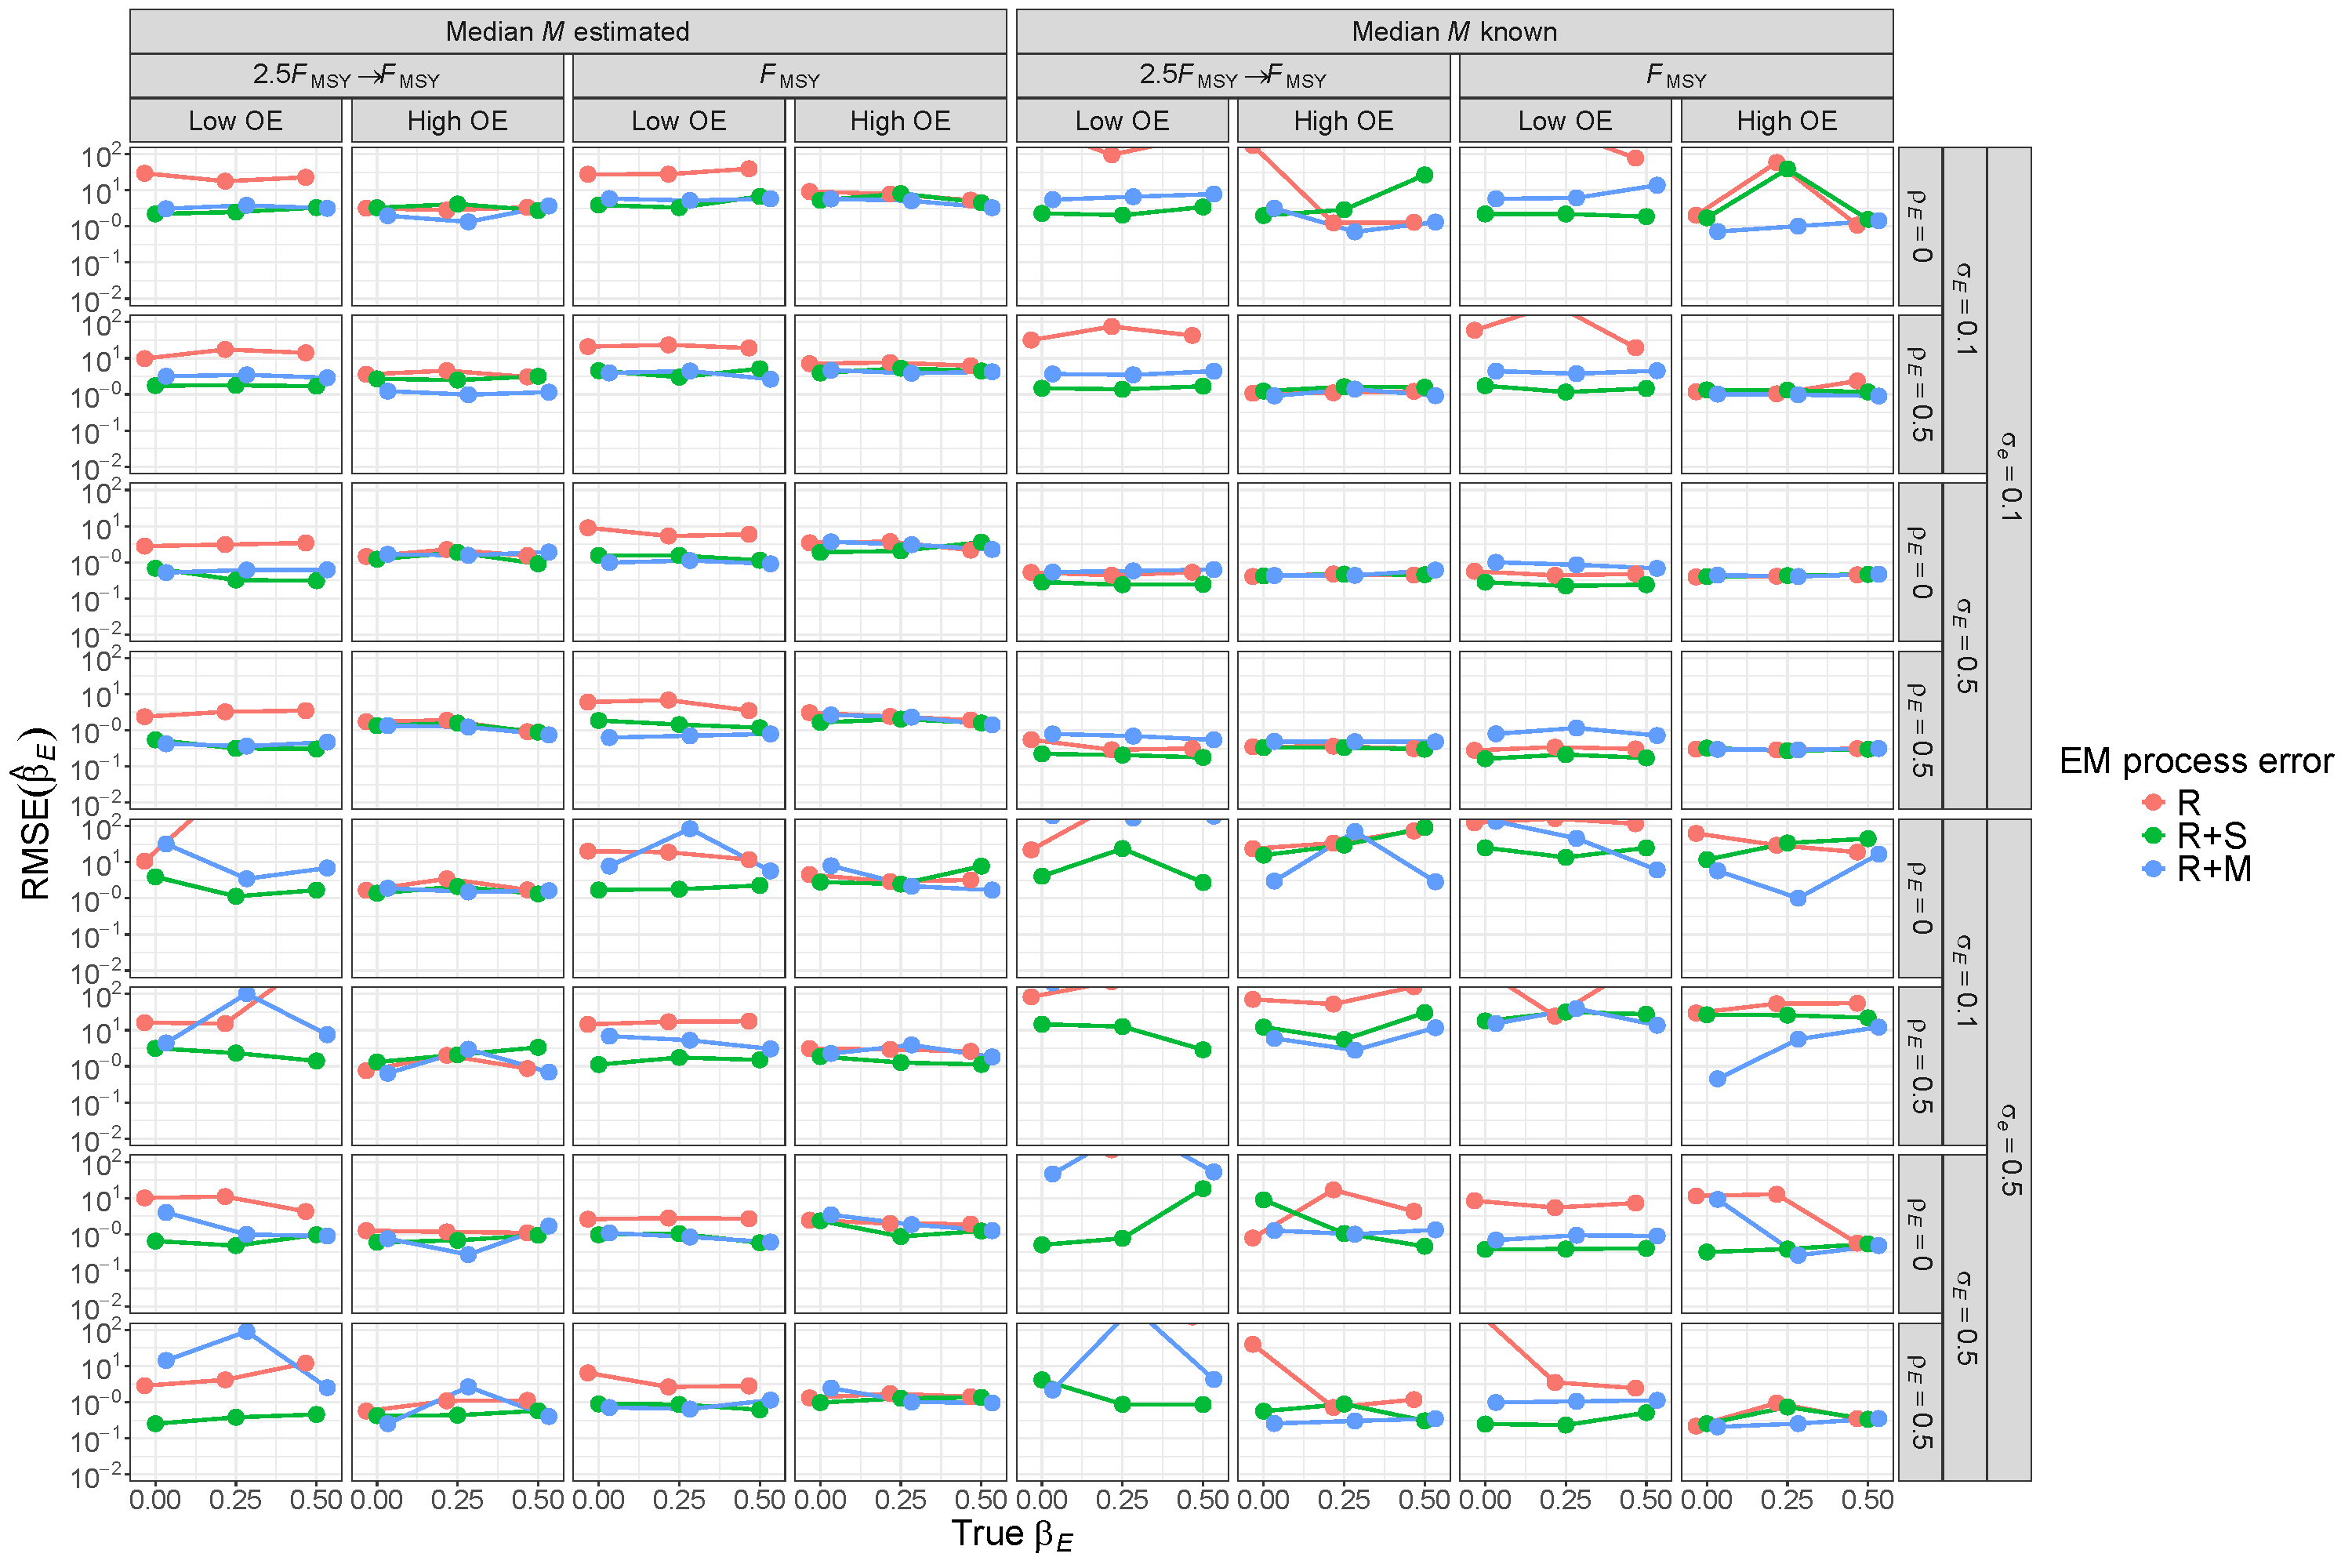
\includegraphics[height = \textheight]{beta_E_rmse_RSom}
%DIFDELCMD < \end{center}
%DIFDELCMD < %%%
%DIFDELCMD < \caption{%
{%DIFAUXCMD
\DIFdelFL{For R+S OMs, RMSE of estimates of covariate effect on $M$ ($\beta_E$) from fitting EMs with alternative process error assumptions and treatment of median $M$ parameter ($\beta_M$). }}%DIFAUXCMD
%DIFDELCMD < \label{beta_E_rmse_RSom}
%DIFDELCMD < \end{figure}
%DIFDELCMD < \end{landscape}
%DIFDELCMD < 

%DIFDELCMD < \begin{landscape}
%DIFDELCMD < \begin{figure}
%DIFDELCMD < \begin{center}
%DIFDELCMD < 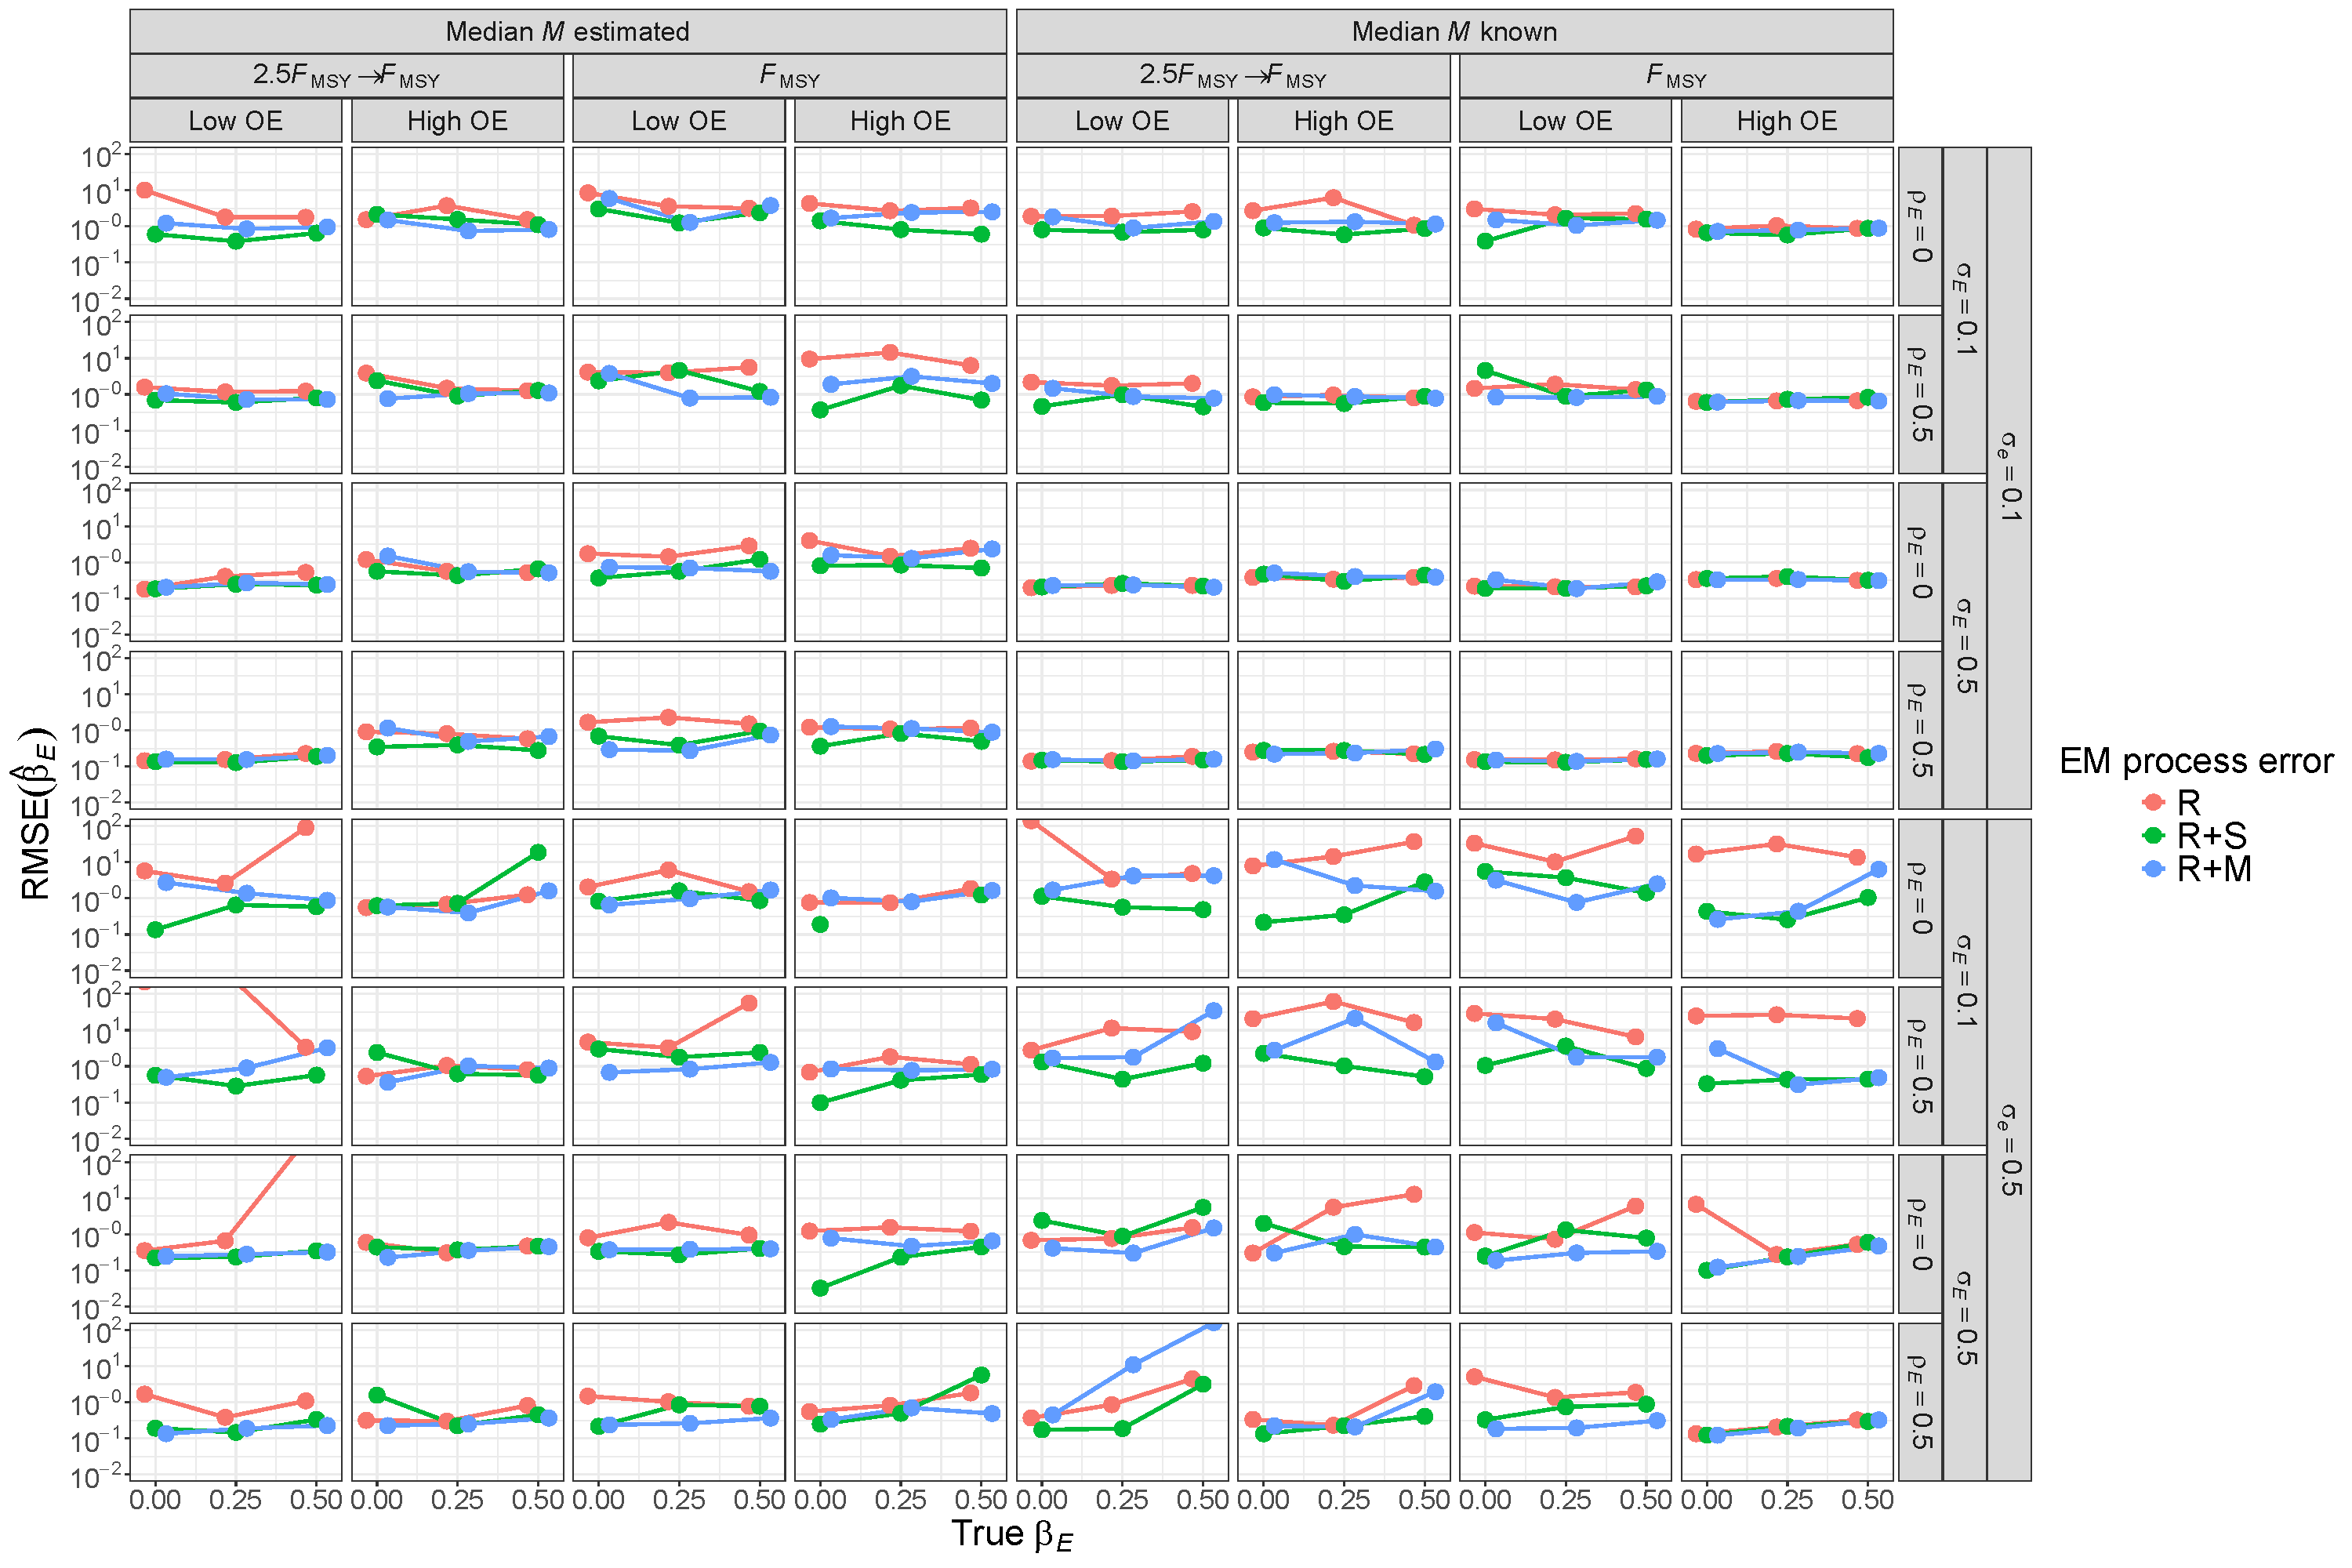
\includegraphics[height = \textheight]{beta_E_rmse_RMom}
%DIFDELCMD < \end{center}
%DIFDELCMD < %%%
%DIFDELCMD < \caption{%
{%DIFAUXCMD
\DIFdelFL{For R+M OMs, RMSE of estimates of covariate effect on $M$ ($\beta_E$) from fitting EMs with alternative process error assumptions and treatment of median $M$ parameter ($\beta_M$). }}%DIFAUXCMD
%DIFDELCMD < \label{beta_E_rmse_RMom}
%DIFDELCMD < \end{figure}
%DIFDELCMD < \end{landscape}
%DIFDELCMD < 

%DIFDELCMD < %%%
\subsection*{\DIFdel{Covariate effect estimate and standard error example}}%DIFAUXCMD
%DIFDELCMD < \label{covariate-effect-estimate-and-standard-error-example}
%DIFDELCMD < %%%
\addcontentsline{toc}{subsection}{\DIFdel{Covariate effect estimate and standard error example}}
%DIFAUXCMD
%DIFDELCMD < 

%DIFDELCMD < \begin{landscape}
%DIFDELCMD < \begin{figure}
%DIFDELCMD < \begin{center}
%DIFDELCMD < 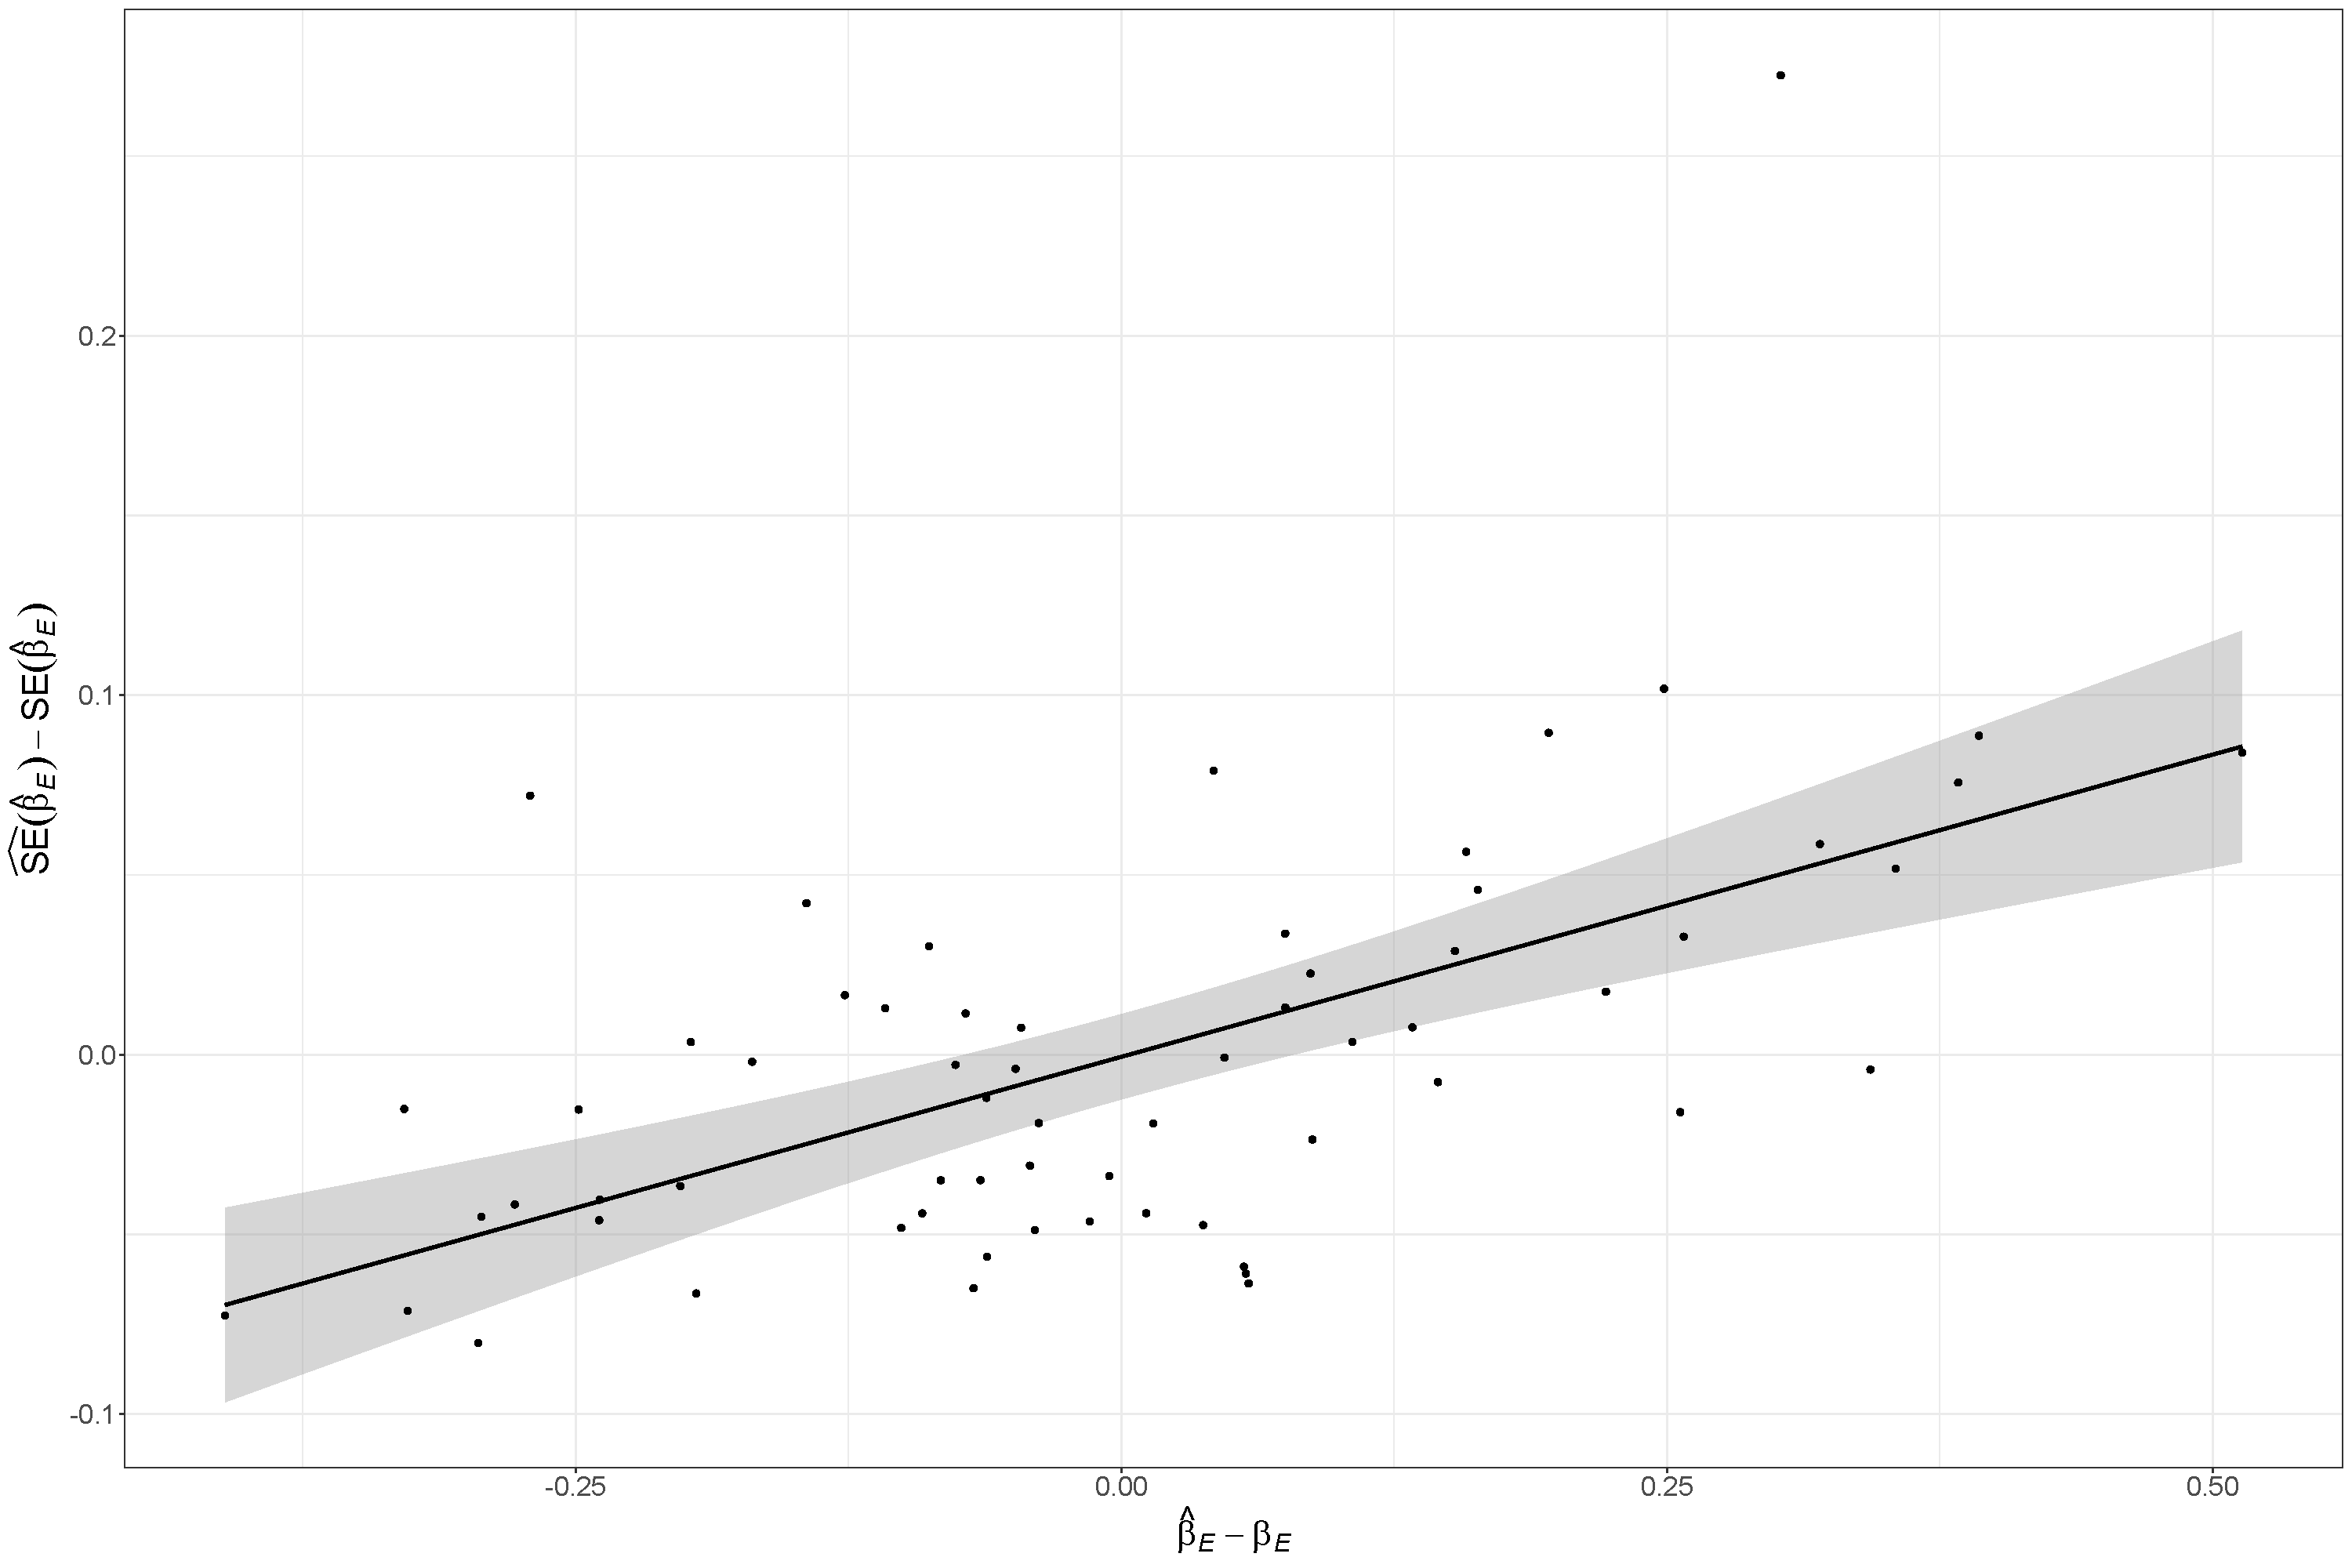
\includegraphics[height = 0.9\textheight]{om_69_em_5_beta_E_se_beta_E_lm_plot}
%DIFDELCMD < \end{center}
%DIFDELCMD < %%%
%DIFDELCMD < \caption{%
{%DIFAUXCMD
\DIFdelFL{Positive correlation of covariate effect estimates and Hessian-based standard error estimates for EM that also estimates the median $M$ parameter ($\beta_M$) and has correct R+M process error assumption fitted to simulated data from the OM with R+M process errors, temporal contrast in fishing pressure, low observation uncertainty for both population ($Low OE$) and covariate observations ($\sigma_e = 0.1$), high and uncorrelated temporal variability in the true covariate ($\sigma_E = 0.5$ and $\rho_E = 0$), and the strongest covariate effect on $M$ ($\beta_E = 0.5$).}}%DIFAUXCMD
%DIFDELCMD < \label{ex_lm_beta_E_SE_beta_E}
%DIFDELCMD < \end{figure}
%DIFDELCMD < \end{landscape}
%DIFDELCMD < 

%DIFDELCMD < %%%
\subsection*{\DIFdel{Median Natural mortality parameter bias}}%DIFAUXCMD
%DIFDELCMD < \label{median-natural-mortality-parameter-bias}
%DIFDELCMD < %%%
\addcontentsline{toc}{subsection}{\DIFdel{Median Natural mortality parameter bias}}
%DIFAUXCMD
%DIFDELCMD < 

%DIFDELCMD < %%%
\DIFdelend \begin{table}
\caption{Percent reduction in deviance for linear regression models fit to \DIFdelbeginFL \DIFdelFL{errors in estimation }\DIFdelendFL \DIFaddbeginFL \DIFaddFL{correlation }\DIFaddendFL of \DIFdelbeginFL \DIFdelFL{the median $M$ parameter }\DIFdelendFL \DIFaddbeginFL \DIFaddFL{terminal year spawning stock biomass }\DIFaddendFL (\DIFdelbeginFL \DIFdelFL{$\beta_M$}\DIFdelendFL \DIFaddbeginFL \DIFaddFL{SSB}\DIFaddendFL ) \DIFdelbeginFL \DIFdelFL{. Table rows give each operating model (OM) }\DIFdelendFL \DIFaddbeginFL \DIFaddFL{estimates }\DIFaddendFL and \DIFdelbeginFL \DIFdelFL{estimating model (EM) factor included individually, combined, and with second and third order interactions}\DIFdelendFL \DIFaddbeginFL \DIFaddFL{true values}\DIFaddendFL . \DIFdelbeginFL \DIFdelFL{Table columns are operating models (OMs) with process error on recruitment only (R), recruitment }\DIFdelendFL \DIFaddbeginFL \DIFaddFL{See Tables \ref{convergence_PRD_table} }\DIFaddendFL and \DIFdelbeginFL \DIFdelFL{apparent survival (R+S), or recruitment and natural mortality (R+M)}\DIFdelendFL \DIFaddbeginFL \DIFaddFL{\ref{factor_table} for further details}\DIFaddendFL .}\DIFdelbeginFL %DIFDELCMD < \label{bias_median_M_complete_PRD_table}
%DIFDELCMD < %%%
\DIFdelendFL \DIFaddbeginFL \label{corr_ssb_PRD_table}
\DIFaddendFL {\begin{center}
\begin{tabular}{lrrr}
\hline\hline
\multicolumn{1}{l}{Factor}&\multicolumn{1}{c}{R}&\multicolumn{1}{c}{R+S}&\multicolumn{1}{c}{R+M}\tabularnewline
\hline
OM $F$ history&\DIFdelbeginFL \DIFdelFL{\textless  0.01}\DIFdelendFL \DIFaddbeginFL \DIFaddFL{19.27}\DIFaddendFL &\DIFdelbeginFL \DIFdelFL{\textless  0.01}\DIFdelendFL \DIFaddbeginFL \DIFaddFL{25.70}\DIFaddendFL &\DIFdelbeginFL \DIFdelFL{\textless  0.01}\DIFdelendFL \DIFaddbeginFL \DIFaddFL{19.59}\DIFaddendFL \tabularnewline
OM Obs. Error&\DIFdelbeginFL \DIFdelFL{\textless  0.01}\DIFdelendFL \DIFaddbeginFL \DIFaddFL{12.53}\DIFaddendFL & \DIFdelbeginFL \DIFdelFL{\textless  0.01}\DIFdelendFL \DIFaddbeginFL \DIFaddFL{3.60}\DIFaddendFL & \DIFdelbeginFL \DIFdelFL{\textless  0.01}\DIFdelendFL \DIFaddbeginFL \DIFaddFL{9.46}\DIFaddendFL \tabularnewline
OM $\sigma_e$& \DIFdelbeginFL \DIFdelFL{\textless  0.01}\DIFdelendFL \DIFaddbeginFL \DIFaddFL{0.08}\DIFaddendFL & \DIFdelbeginFL \DIFdelFL{\textless  0.01}\DIFdelendFL \DIFaddbeginFL \DIFaddFL{0.44}\DIFaddendFL & \DIFdelbeginFL \DIFdelFL{\textless  0.01}\DIFdelendFL \DIFaddbeginFL \DIFaddFL{0.09}\DIFaddendFL \tabularnewline
OM $\sigma_E$& \DIFdelbeginFL \DIFdelFL{\textless  0.01}\DIFdelendFL \DIFaddbeginFL \DIFaddFL{0.10}\DIFaddendFL & \DIFdelbeginFL \DIFdelFL{\textless  0.01}\DIFdelendFL \DIFaddbeginFL \DIFaddFL{0.44}\DIFaddendFL & \DIFdelbeginFL \DIFdelFL{\textless  0.01}\DIFdelendFL \DIFaddbeginFL \DIFaddFL{0.11}\DIFaddendFL \tabularnewline
OM $\rho_{E}$&\textless  0.01&\textless  0.01& \DIFdelbeginFL \DIFdelFL{\textless  0.01}\DIFdelendFL \DIFaddbeginFL \DIFaddFL{0.09}\DIFaddendFL \tabularnewline
OM $\beta_{E}$& \DIFdelbeginFL \DIFdelFL{\textless  0.01}\DIFdelendFL \DIFaddbeginFL \DIFaddFL{0.09}\DIFaddendFL & \DIFdelbeginFL \DIFdelFL{\textless  0.01}\DIFdelendFL \DIFaddbeginFL \DIFaddFL{0.05}\DIFaddendFL &\DIFdelbeginFL \DIFdelFL{0.01}%DIFDELCMD < \tabularnewline
%DIFDELCMD < %%%
\DIFdelFL{EM Convergence}%DIFDELCMD < &%%%
\DIFdelendFL \textless  0.01\DIFdelbeginFL %DIFDELCMD < &%%%
\DIFdelFL{0.01}%DIFDELCMD < &%%%
\DIFdelFL{0.01}\DIFdelendFL \tabularnewline
EM Process Error& \DIFdelbeginFL \DIFdelFL{\textless  0.01}\DIFdelendFL \DIFaddbeginFL \DIFaddFL{0.07}\DIFaddendFL & \DIFdelbeginFL \DIFdelFL{0.01}\DIFdelendFL \DIFaddbeginFL \DIFaddFL{0.92}\DIFaddendFL & \DIFdelbeginFL \DIFdelFL{0.01}\DIFdelendFL \DIFaddbeginFL \DIFaddFL{0.71}\DIFaddendFL \tabularnewline
\DIFdelbeginFL \DIFdelFL{EM $\beta_{E}$ }\DIFdelendFL \DIFaddbeginFL \DIFaddFL{$EM \beta_{E}$ }\DIFaddendFL assumption&\textless  0.01& \DIFdelbeginFL \DIFdelFL{\textless  0.01}\DIFdelendFL \DIFaddbeginFL \DIFaddFL{1.32}\DIFaddendFL & \DIFdelbeginFL \DIFdelFL{\textless  0.01}\DIFdelendFL \DIFaddbeginFL \DIFaddFL{0.38}\DIFaddendFL \tabularnewline
\DIFdelbeginFL \DIFdelFL{All factors}%DIFDELCMD < &%%%
\DIFdelFL{0.02}%DIFDELCMD < &%%%
\DIFdelFL{0.02}%DIFDELCMD < &%%%
\DIFdelFL{0.05}%DIFDELCMD < \tabularnewline
%DIFDELCMD < %%%
\DIFdelFL{+ All Two Way}%DIFDELCMD < &%%%
\DIFdelFL{0.15}%DIFDELCMD < &%%%
\DIFdelFL{0.15}%DIFDELCMD < &%%%
\DIFdelFL{0.24}%DIFDELCMD < \tabularnewline
%DIFDELCMD < %%%
\DIFdelFL{+ All Three Way}%DIFDELCMD < &%%%
\DIFdelFL{0.57}%DIFDELCMD < &%%%
\DIFdelFL{0.54}%DIFDELCMD < &%%%
\DIFdelFL{0.73}%DIFDELCMD < \tabularnewline
%DIFDELCMD < \hline
%DIFDELCMD < \end{tabular}\end{center}
%DIFDELCMD < }
%DIFDELCMD < \end{table}
%DIFDELCMD < 

%DIFDELCMD < \begin{landscape}
%DIFDELCMD < \begin{figure}
%DIFDELCMD < \begin{center}
%DIFDELCMD < 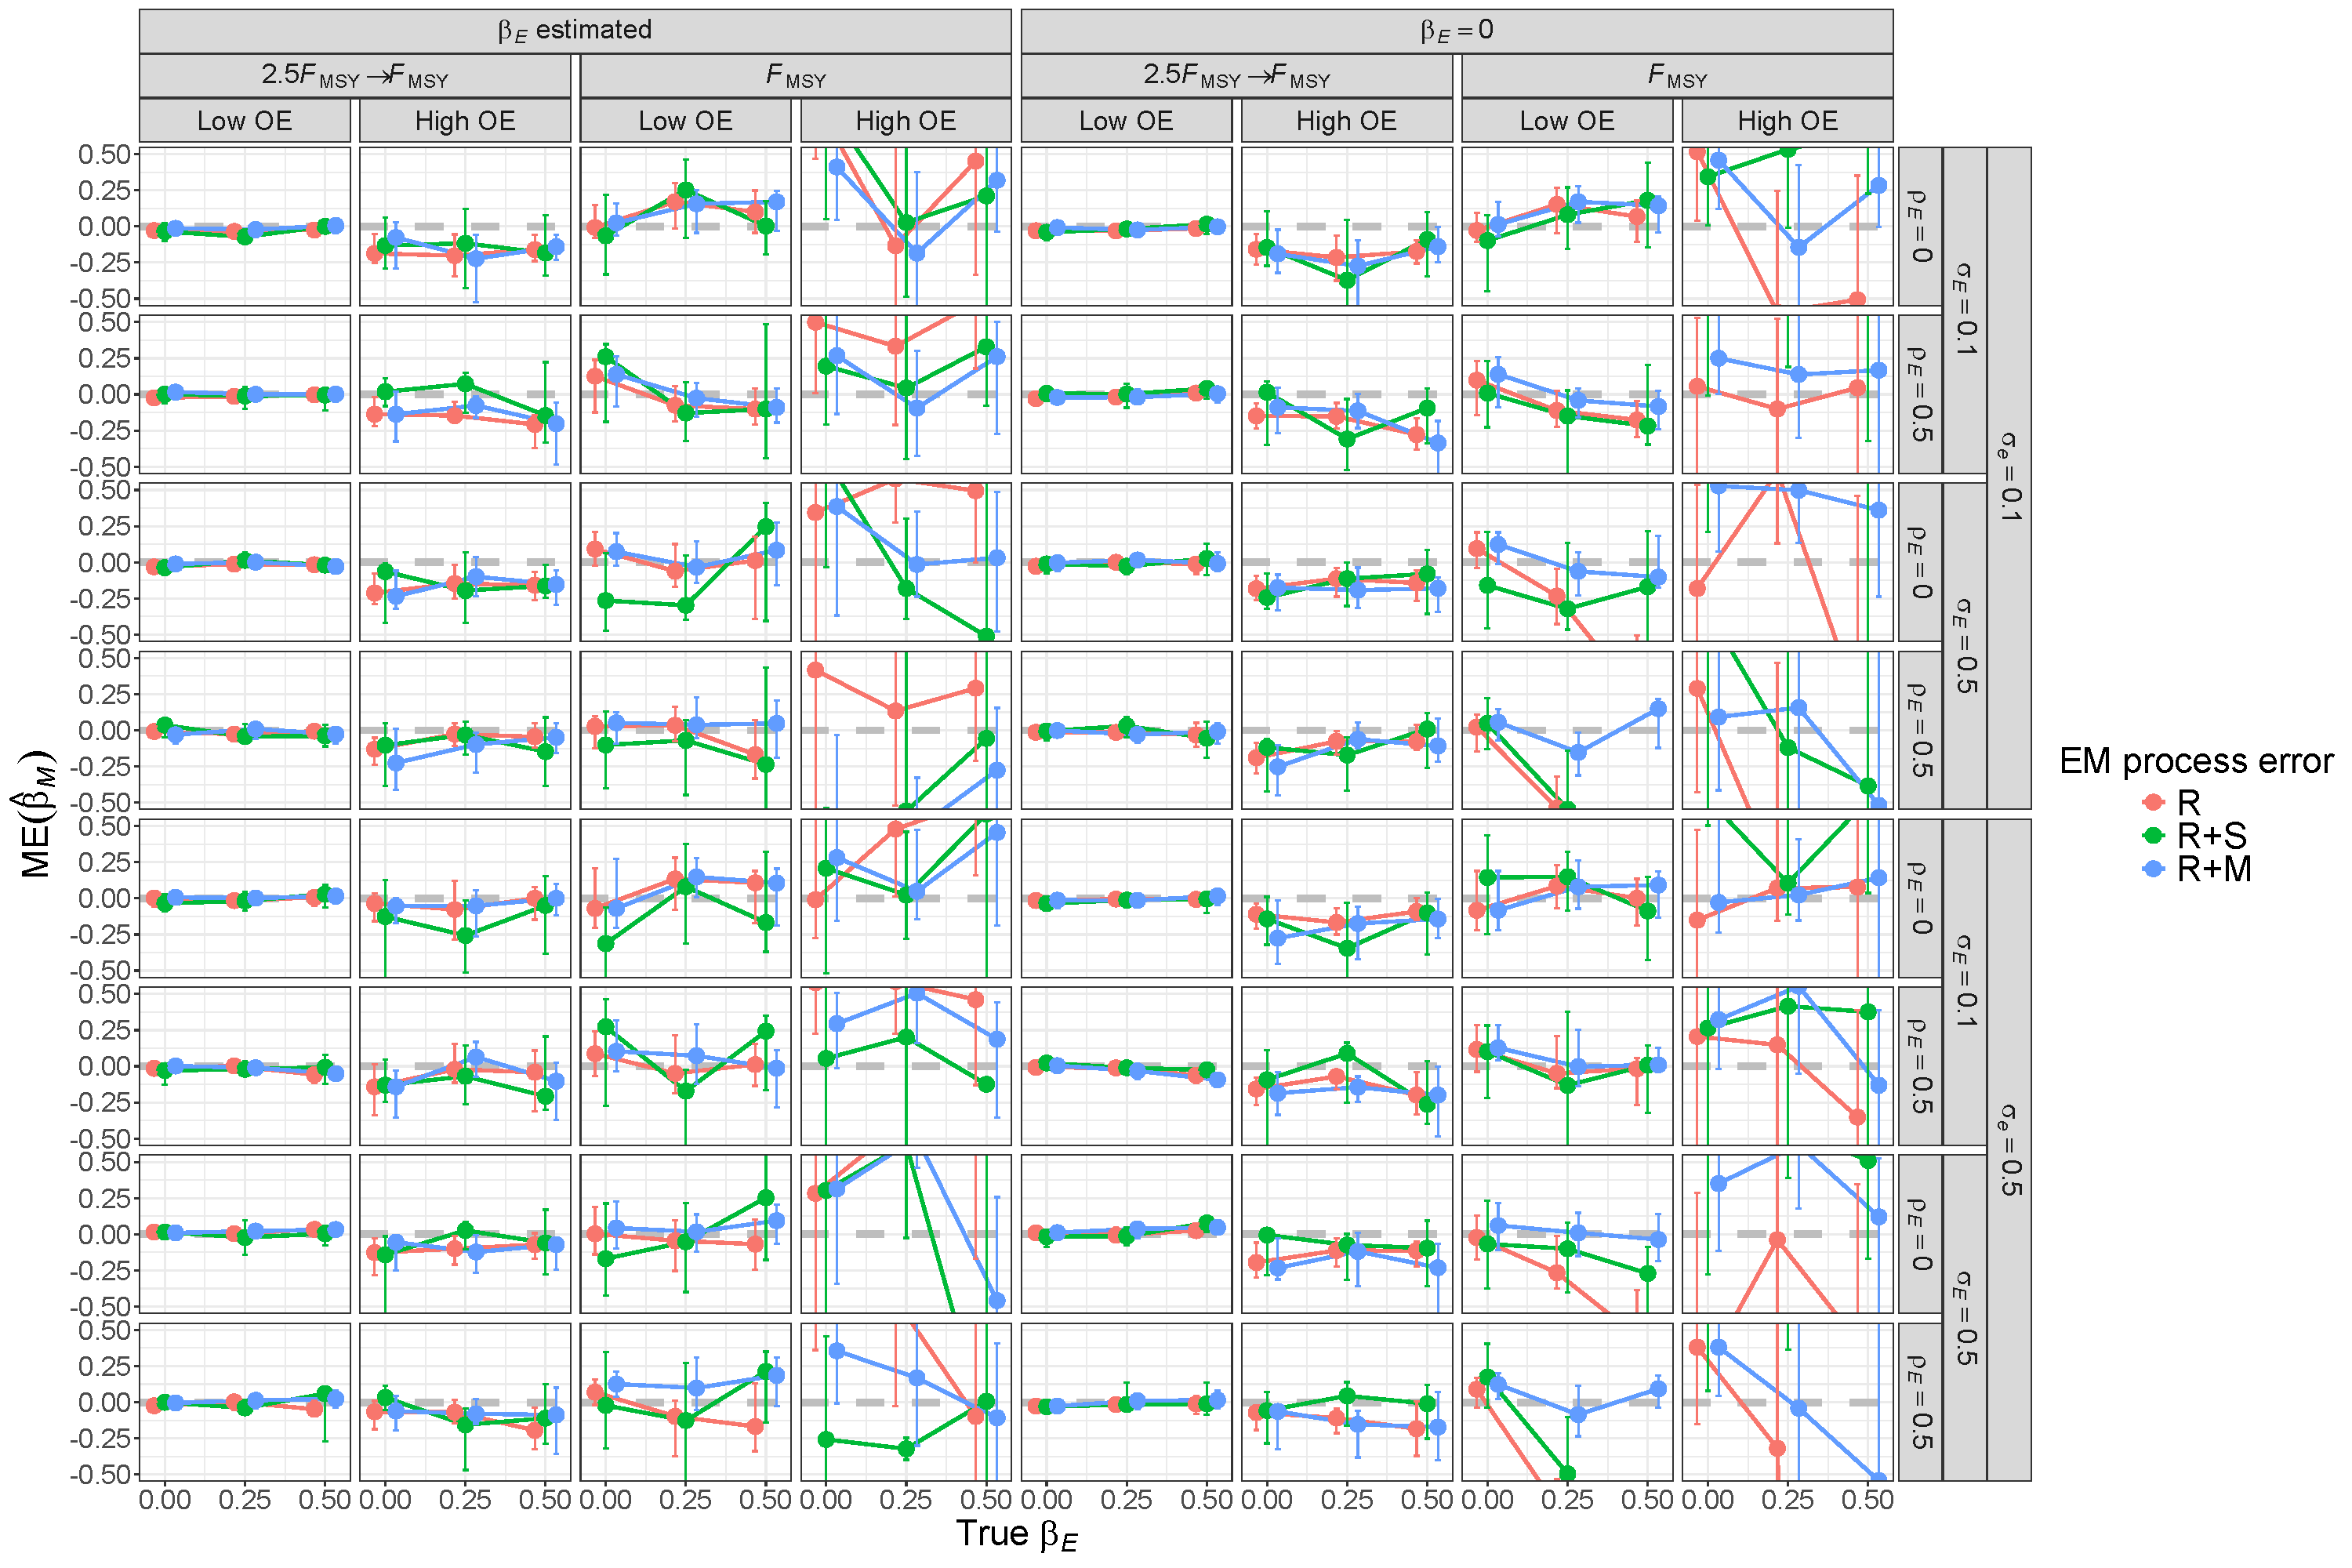
\includegraphics[height = \textheight]{beta_M_bias_Rom}
%DIFDELCMD < \end{center}
%DIFDELCMD < %%%
%DIFDELCMD < \caption{%
{%DIFAUXCMD
\DIFdelFL{For R OMs, median error (ME) of estimates of $\beta_M$ from fitting EMs with alternative process error assumptions and treatment of covariate effect ($\beta_E = 0$ or estimated). Vertical lines represent 95\% confidence intervals.}}%DIFAUXCMD
%DIFDELCMD < \label{beta_M_bias_Rom}
%DIFDELCMD < \end{figure}
%DIFDELCMD < \end{landscape}
%DIFDELCMD < 

%DIFDELCMD < \begin{landscape}
%DIFDELCMD < \begin{figure}
%DIFDELCMD < \begin{center}
%DIFDELCMD < 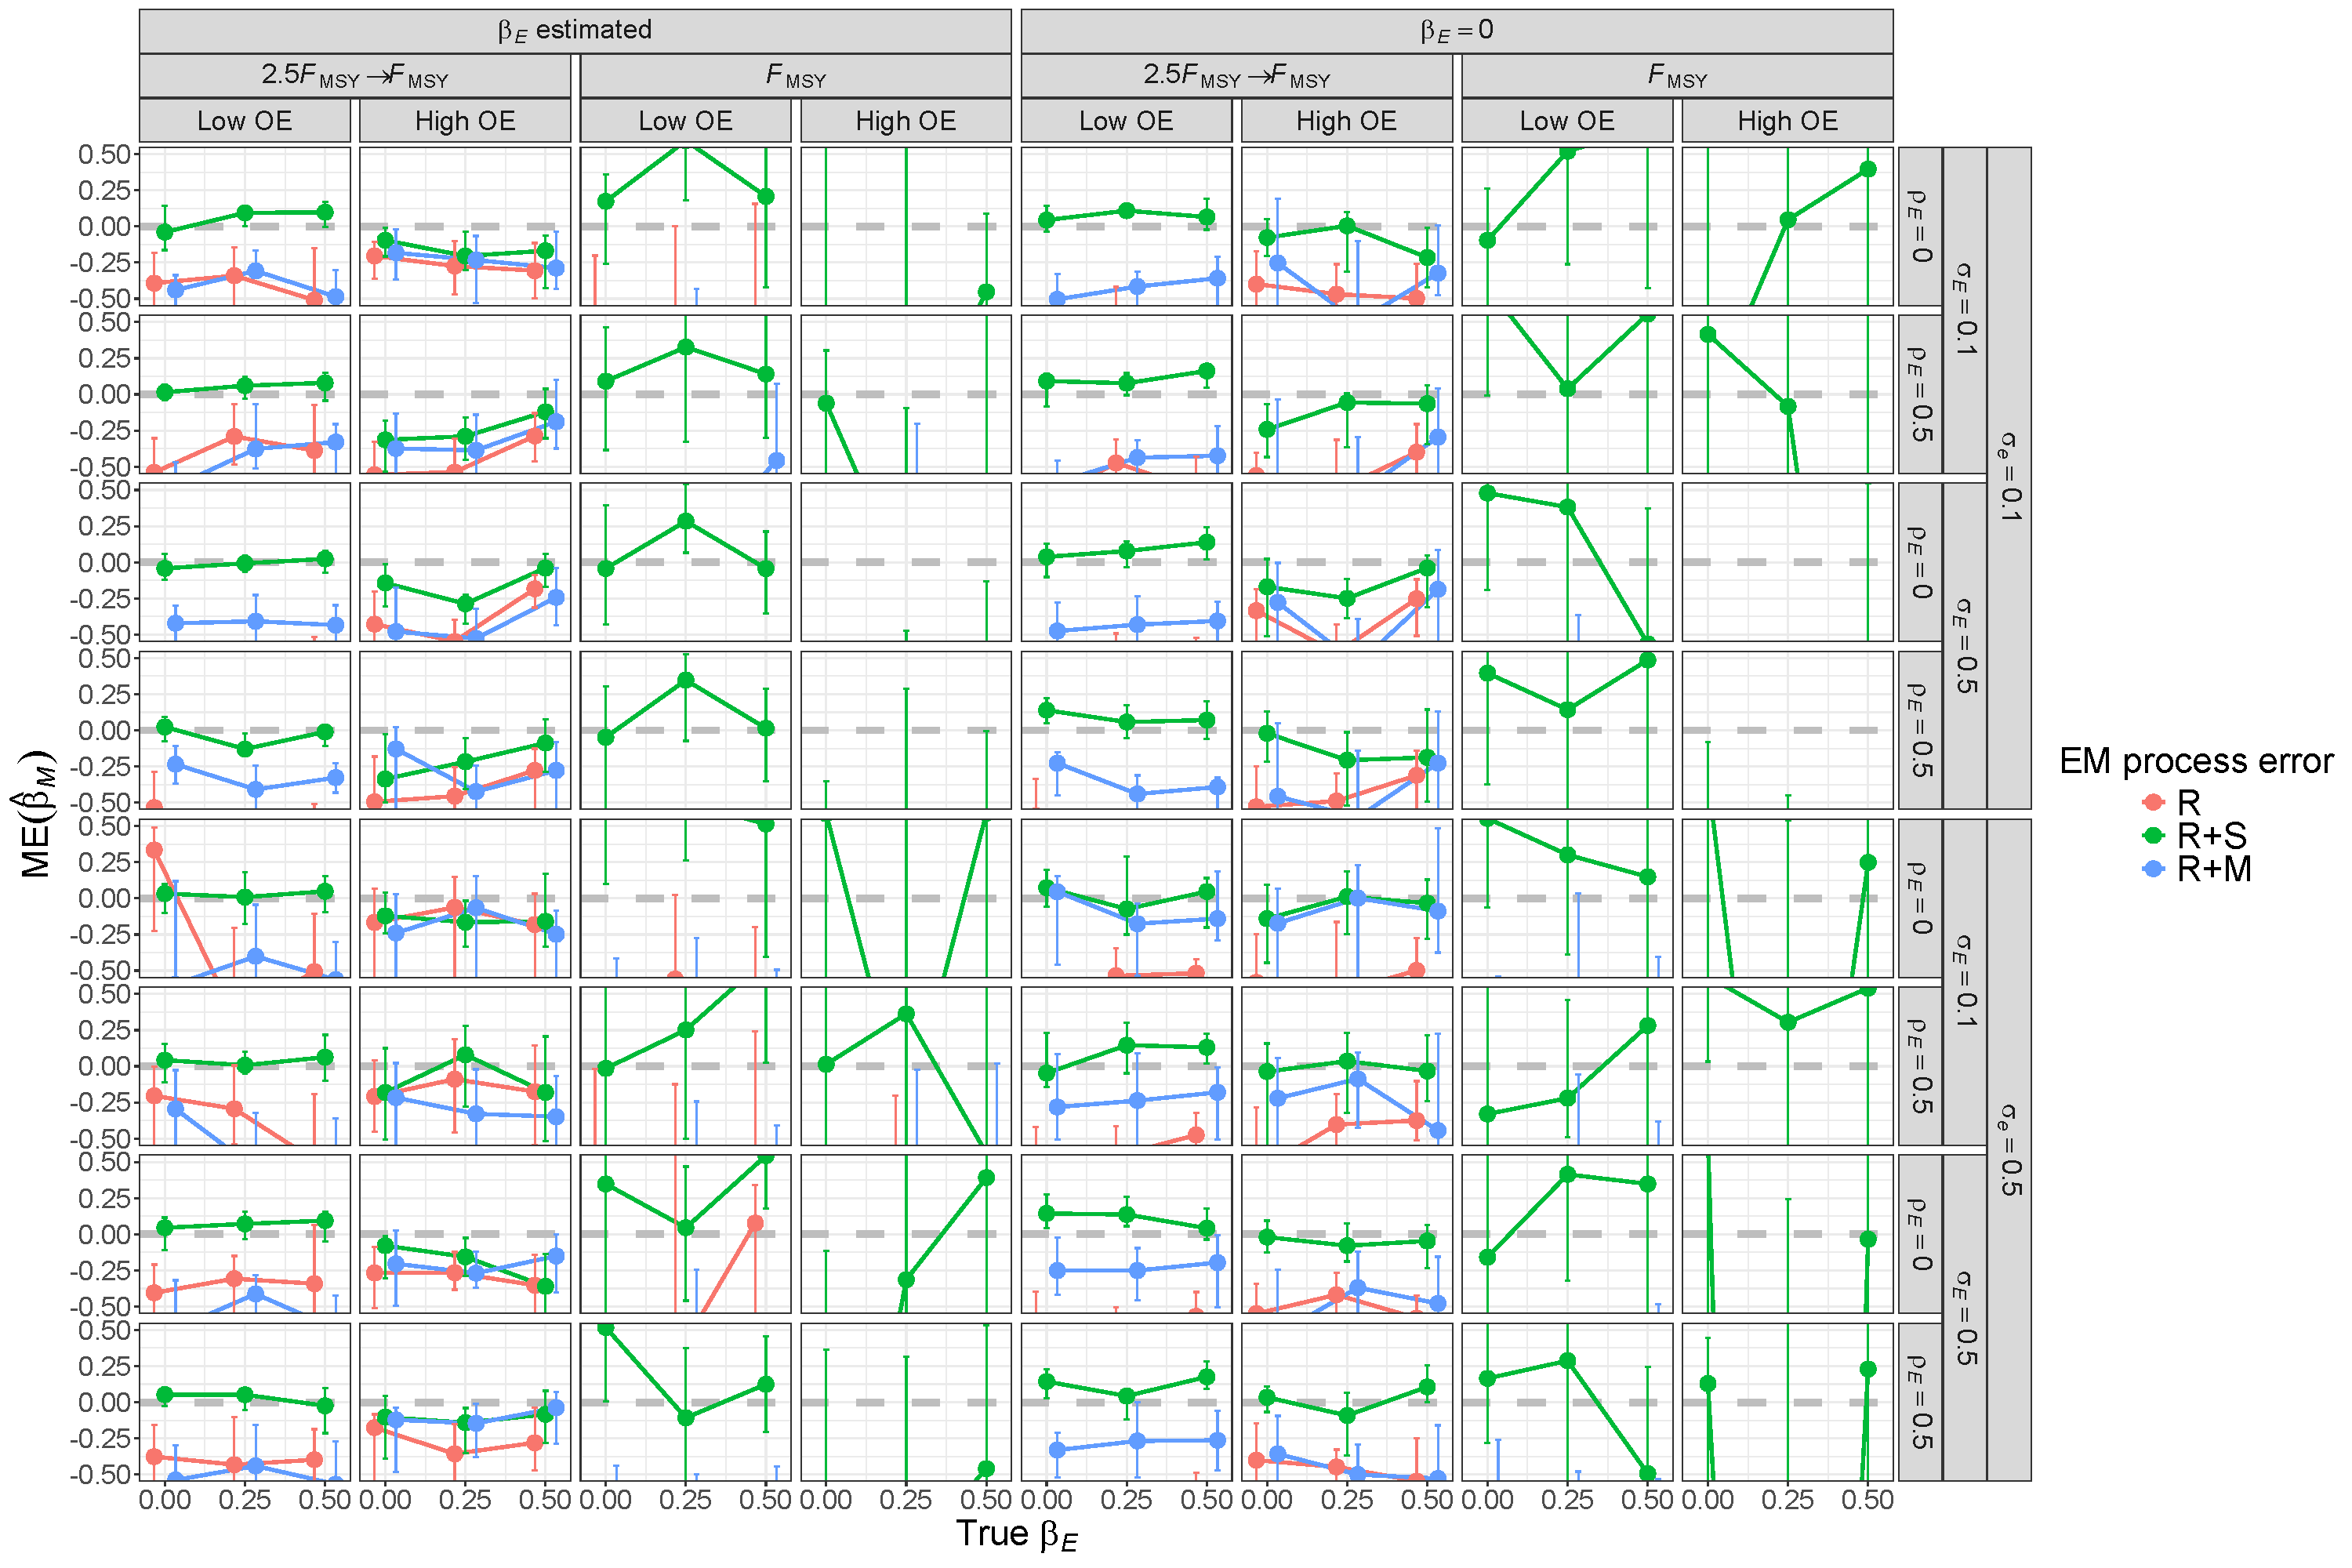
\includegraphics[height = \textheight]{beta_M_bias_RSom}
%DIFDELCMD < \end{center}
%DIFDELCMD < %%%
%DIFDELCMD < \caption{%
{%DIFAUXCMD
\DIFdelFL{For R+S OMs, median error (ME) of estimates of $\beta_M$ from fitting EMs with alternative process error assumptions and treatment of covariate effect ($\beta_E = 0$ or estimated). Vertical lines represent 95\% confidence intervals.}}%DIFAUXCMD
%DIFDELCMD < \label{beta_M_bias_RSom}
%DIFDELCMD < \end{figure}
%DIFDELCMD < \end{landscape}
%DIFDELCMD < 

%DIFDELCMD < \begin{landscape}
%DIFDELCMD < \begin{figure}
%DIFDELCMD < \begin{center}
%DIFDELCMD < 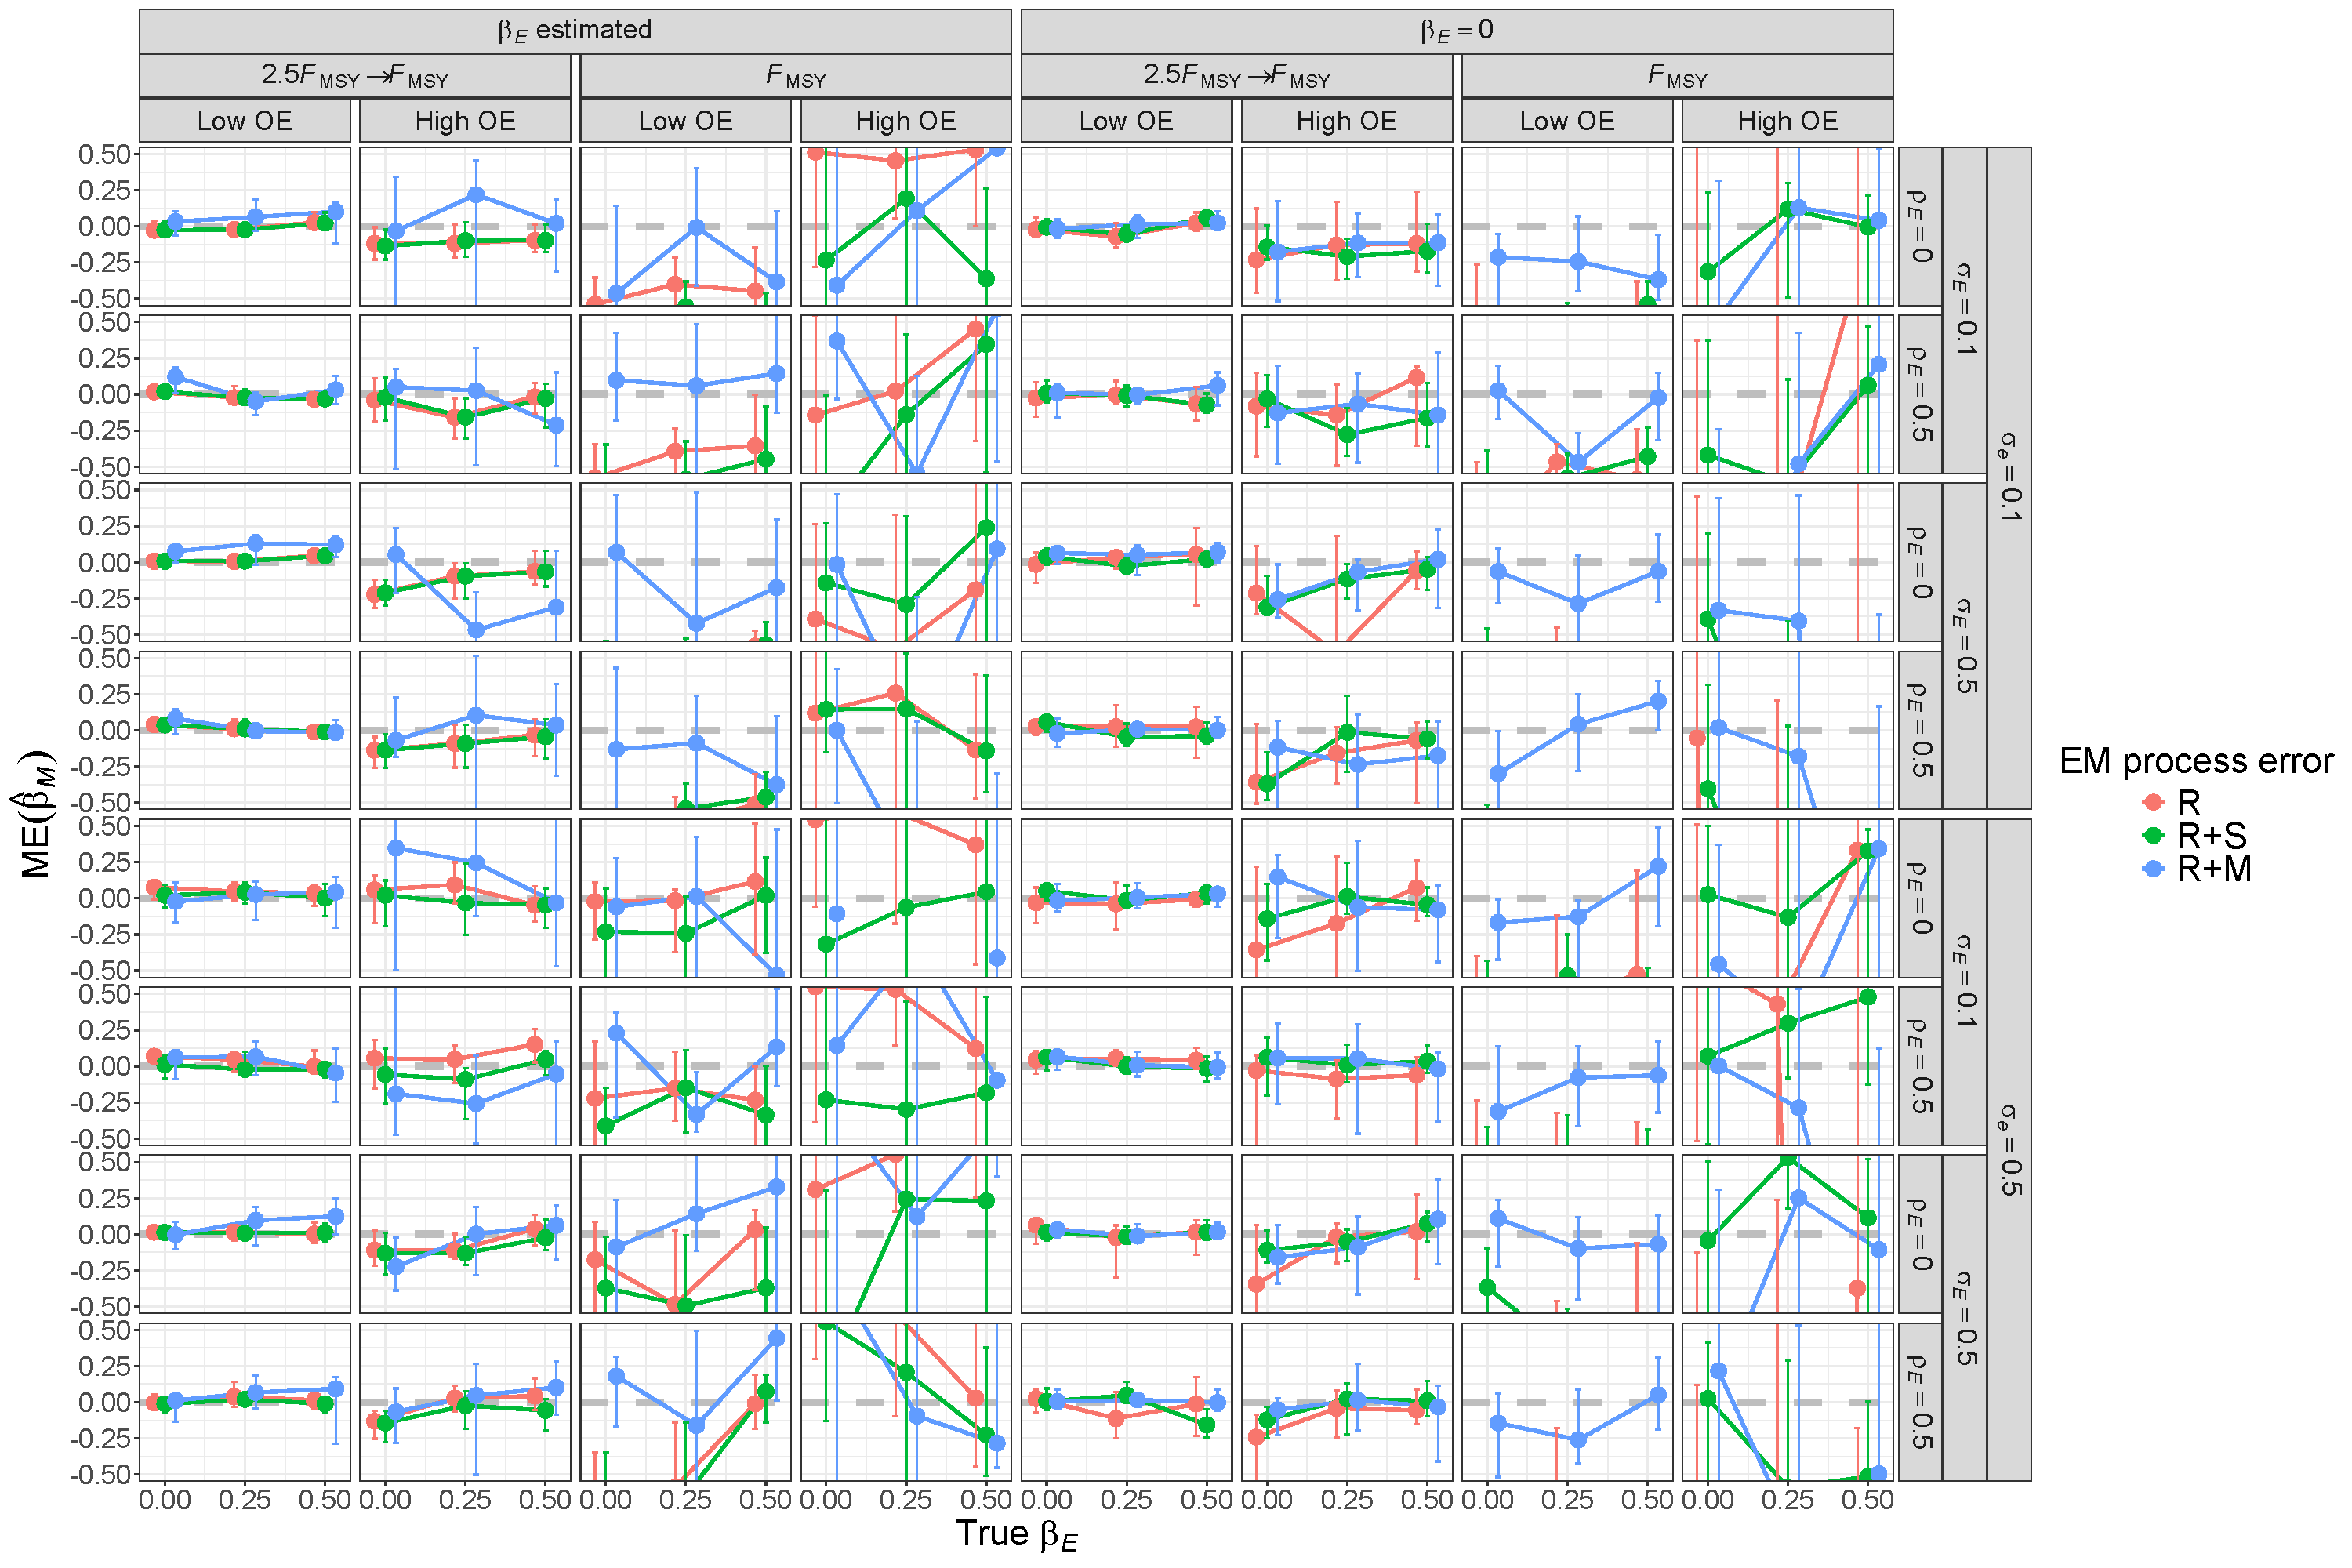
\includegraphics[height = \textheight]{beta_M_bias_RMom}
%DIFDELCMD < \end{center}
%DIFDELCMD < %%%
%DIFDELCMD < \caption{%
{%DIFAUXCMD
\DIFdelFL{For R+M OMs, median error (ME) of estimates of $\beta_M$ from fitting EMs with alternative process error assumptions and treatment of covariate effect ($\beta_E = 0$ or estimated). Vertical lines represent 95\% confidence intervals.}}%DIFAUXCMD
%DIFDELCMD < \label{beta_M_bias_RMom}
%DIFDELCMD < \end{figure}
%DIFDELCMD < \end{landscape}
%DIFDELCMD < 

%DIFDELCMD < %%%
\subsection*{\DIFdel{Median natural mortality parameter standard error estimation bias}}%DIFAUXCMD
%DIFDELCMD < \label{median-natural-mortality-parameter-standard-error-estimation-bias}
%DIFDELCMD < %%%
\addcontentsline{toc}{subsection}{\DIFdel{Median natural mortality parameter standard error estimation bias}}
%DIFAUXCMD
%DIFDELCMD < 

%DIFDELCMD < \begin{landscape}
%DIFDELCMD < \begin{figure}
%DIFDELCMD < \begin{center}
%DIFDELCMD < 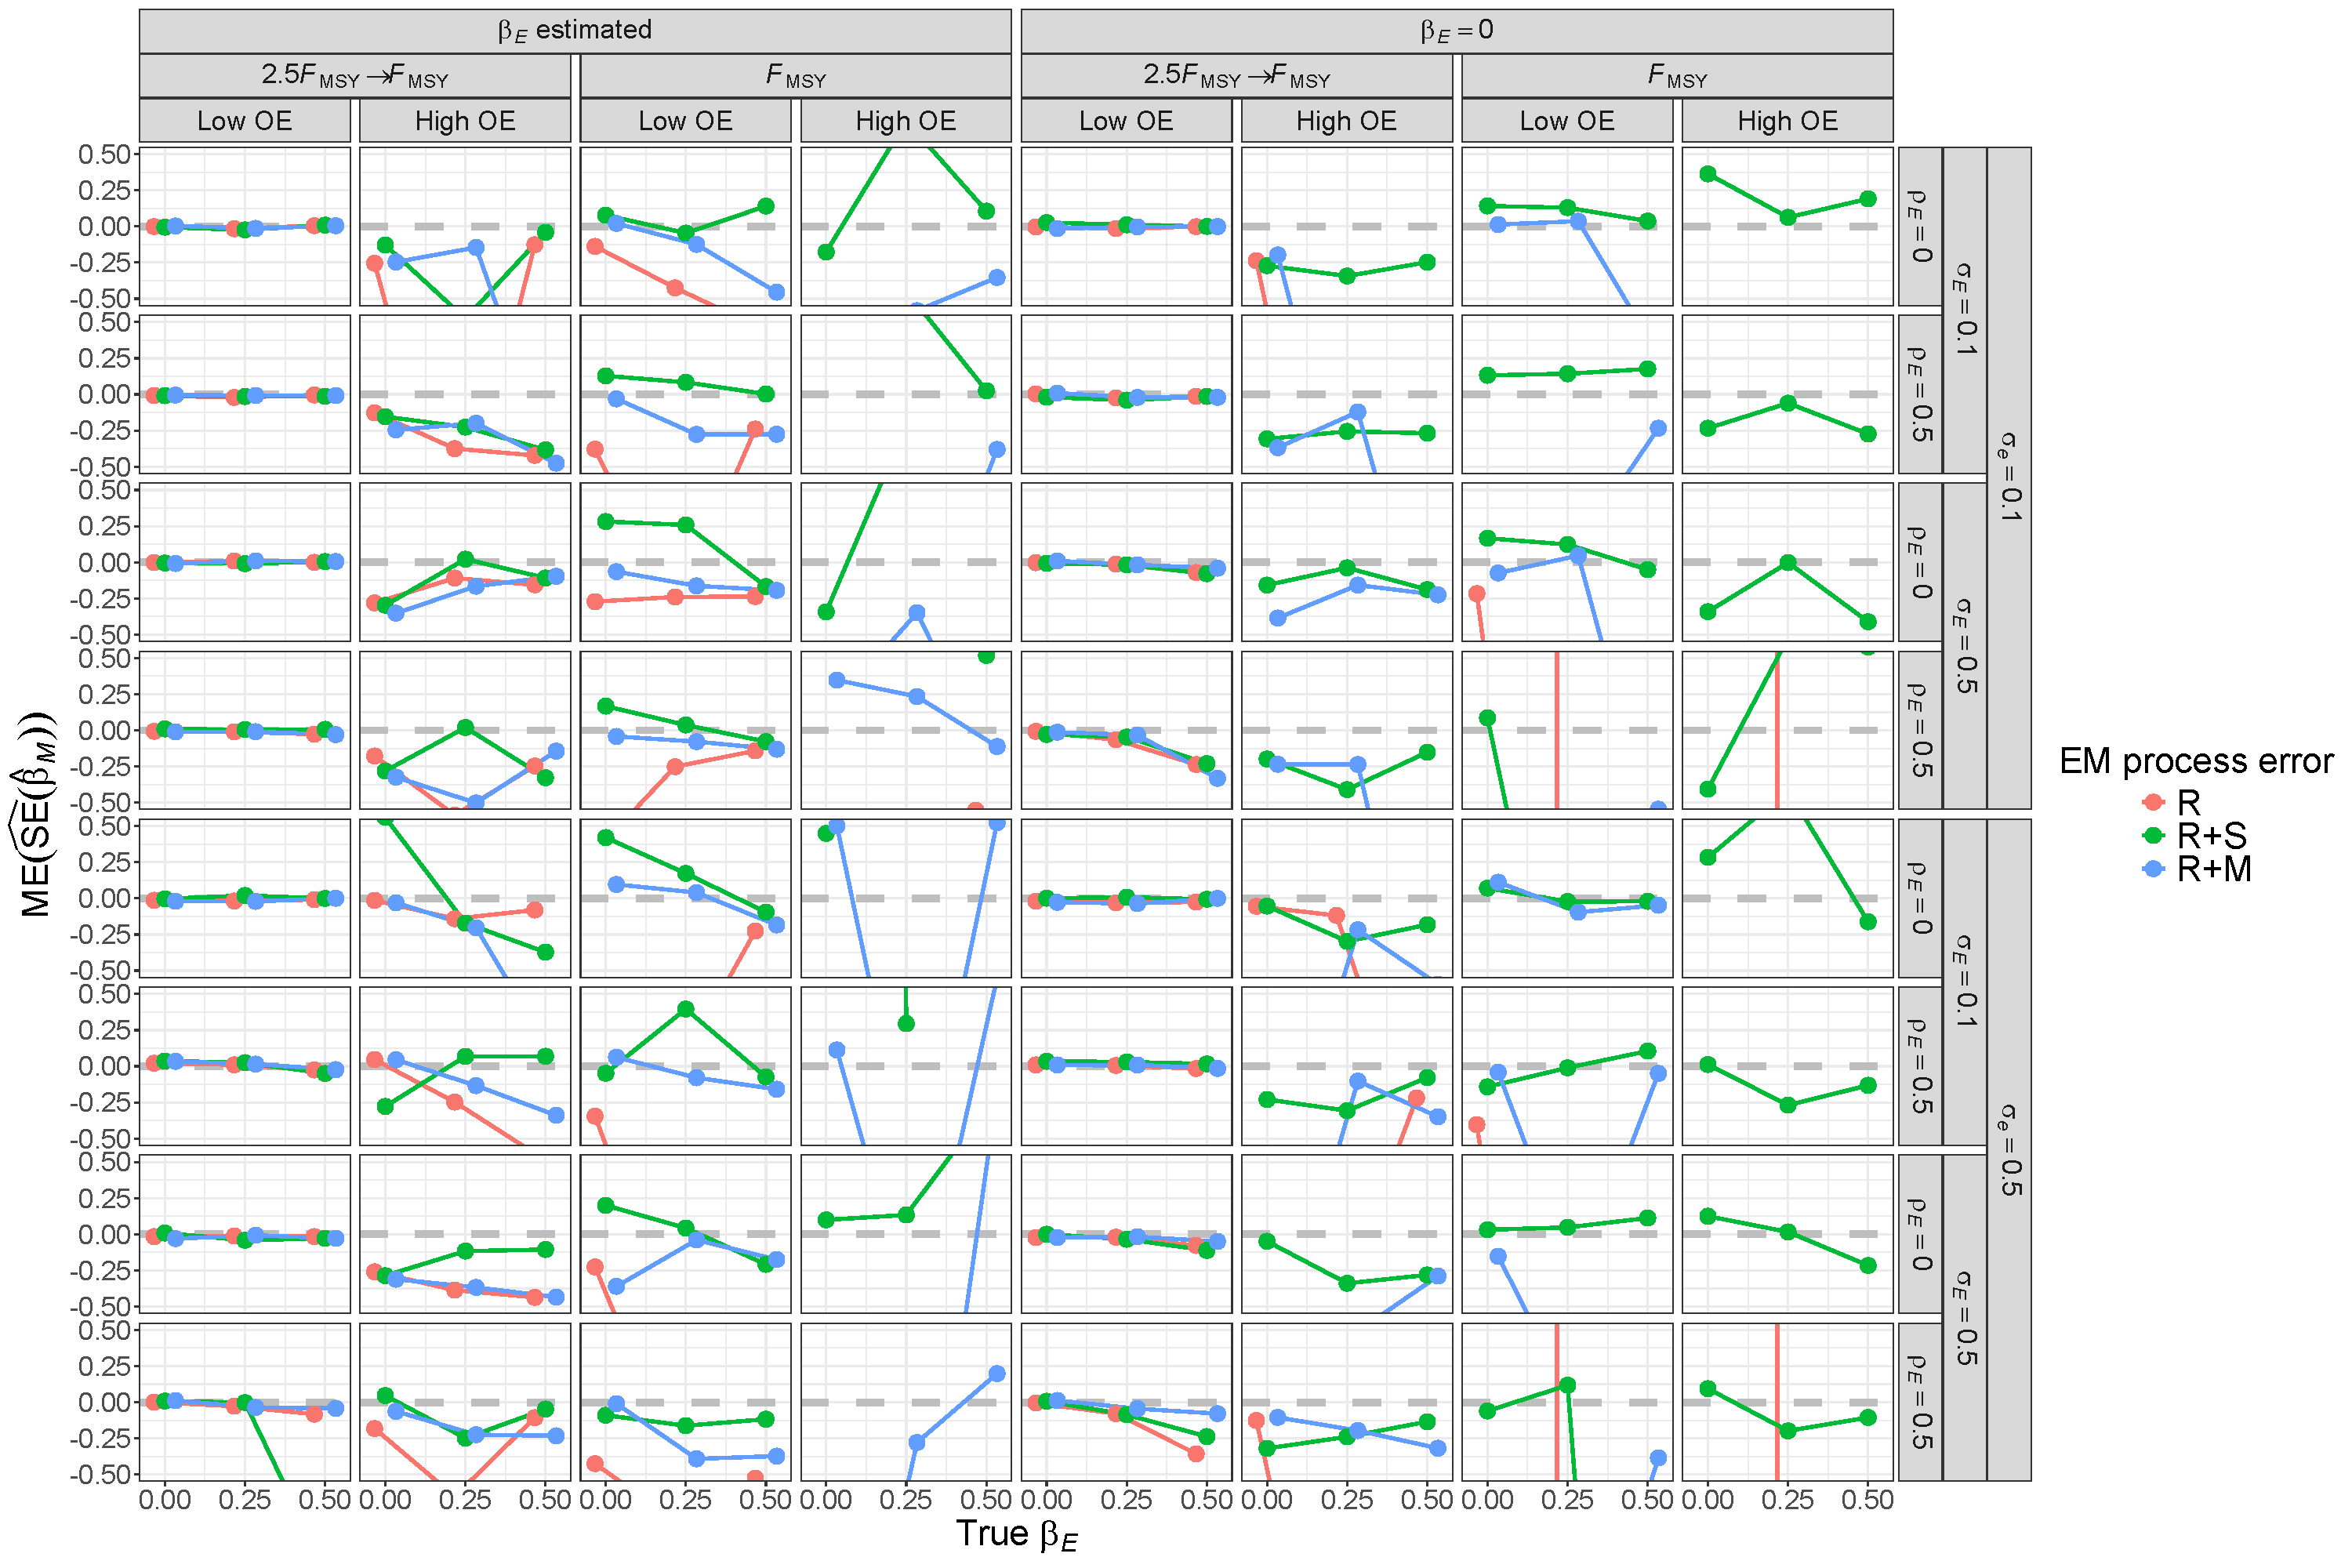
\includegraphics[height = \textheight]{se_beta_M_bias_Rom}
%DIFDELCMD < \end{center}
%DIFDELCMD < %%%
%DIFDELCMD < \caption{%
{%DIFAUXCMD
\DIFdelFL{For R OMs, median error (ME) of Hessian-based estimates of standard error for median $M$ parameter ($\beta_M$) from fitting EMs with alternative process error assumptions and treatment of the covariate effect ($\beta_ E= 0$ or estimated). True standard error is defined as the mean of the standard error estimates accross converged fits to simulated data sets for a given OM scenario.}}%DIFAUXCMD
%DIFDELCMD < \label{se_beta_M_bias_Rom}
%DIFDELCMD < \end{figure}
%DIFDELCMD < \end{landscape}
%DIFDELCMD < 

%DIFDELCMD < \begin{landscape}
%DIFDELCMD < \begin{figure}
%DIFDELCMD < \begin{center}
%DIFDELCMD < 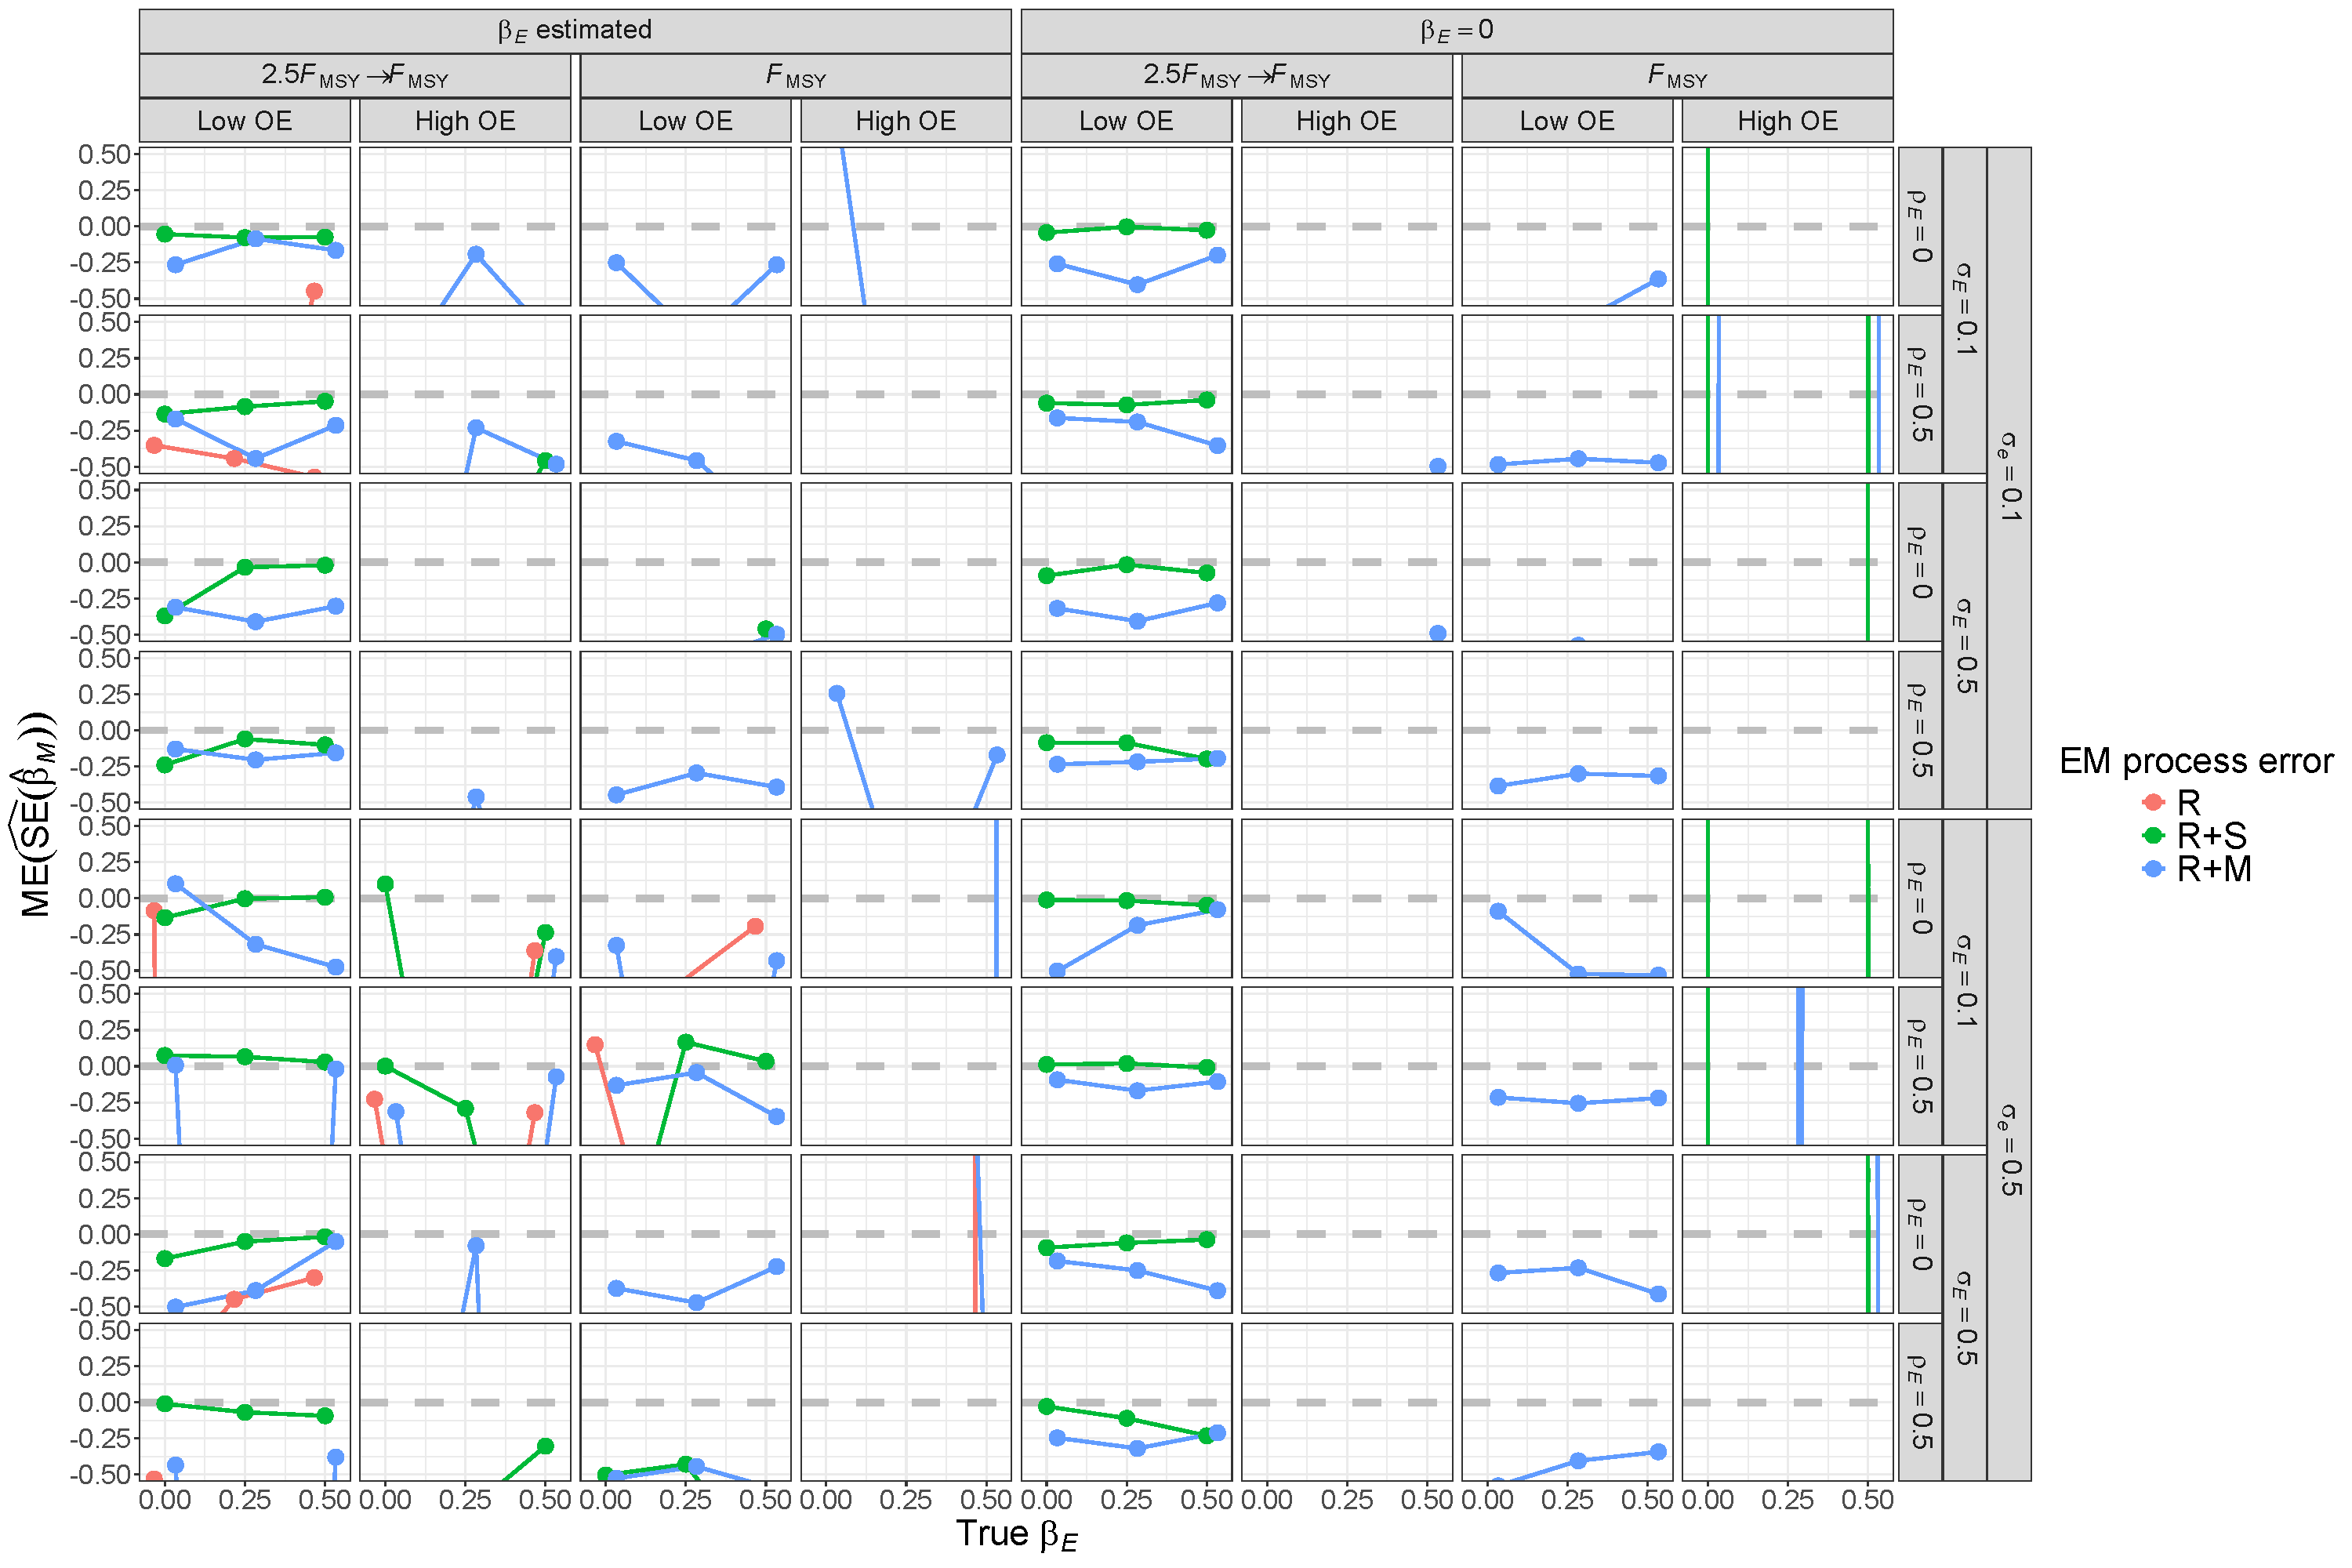
\includegraphics[height = \textheight]{se_beta_M_bias_RSom}
%DIFDELCMD < \end{center}
%DIFDELCMD < %%%
%DIFDELCMD < \caption{%
{%DIFAUXCMD
\DIFdelFL{For R+S OMs, median error (ME) of Hessian-based estimates of standard error for median $M$ parameter ($\beta_M$) from fitting EMs with alternative process error assumptions and treatment of the covariate effect ($\beta_ E= 0$ or estimated). True standard error is defined as the mean of the standard error estimates accross converged fits to simulated data sets for a given OM scenario.}}%DIFAUXCMD
%DIFDELCMD < \label{se_beta_M_bias_RSom}
%DIFDELCMD < \end{figure}
%DIFDELCMD < \end{landscape}
%DIFDELCMD < 

%DIFDELCMD < \begin{landscape}
%DIFDELCMD < \begin{figure}
%DIFDELCMD < \begin{center}
%DIFDELCMD < 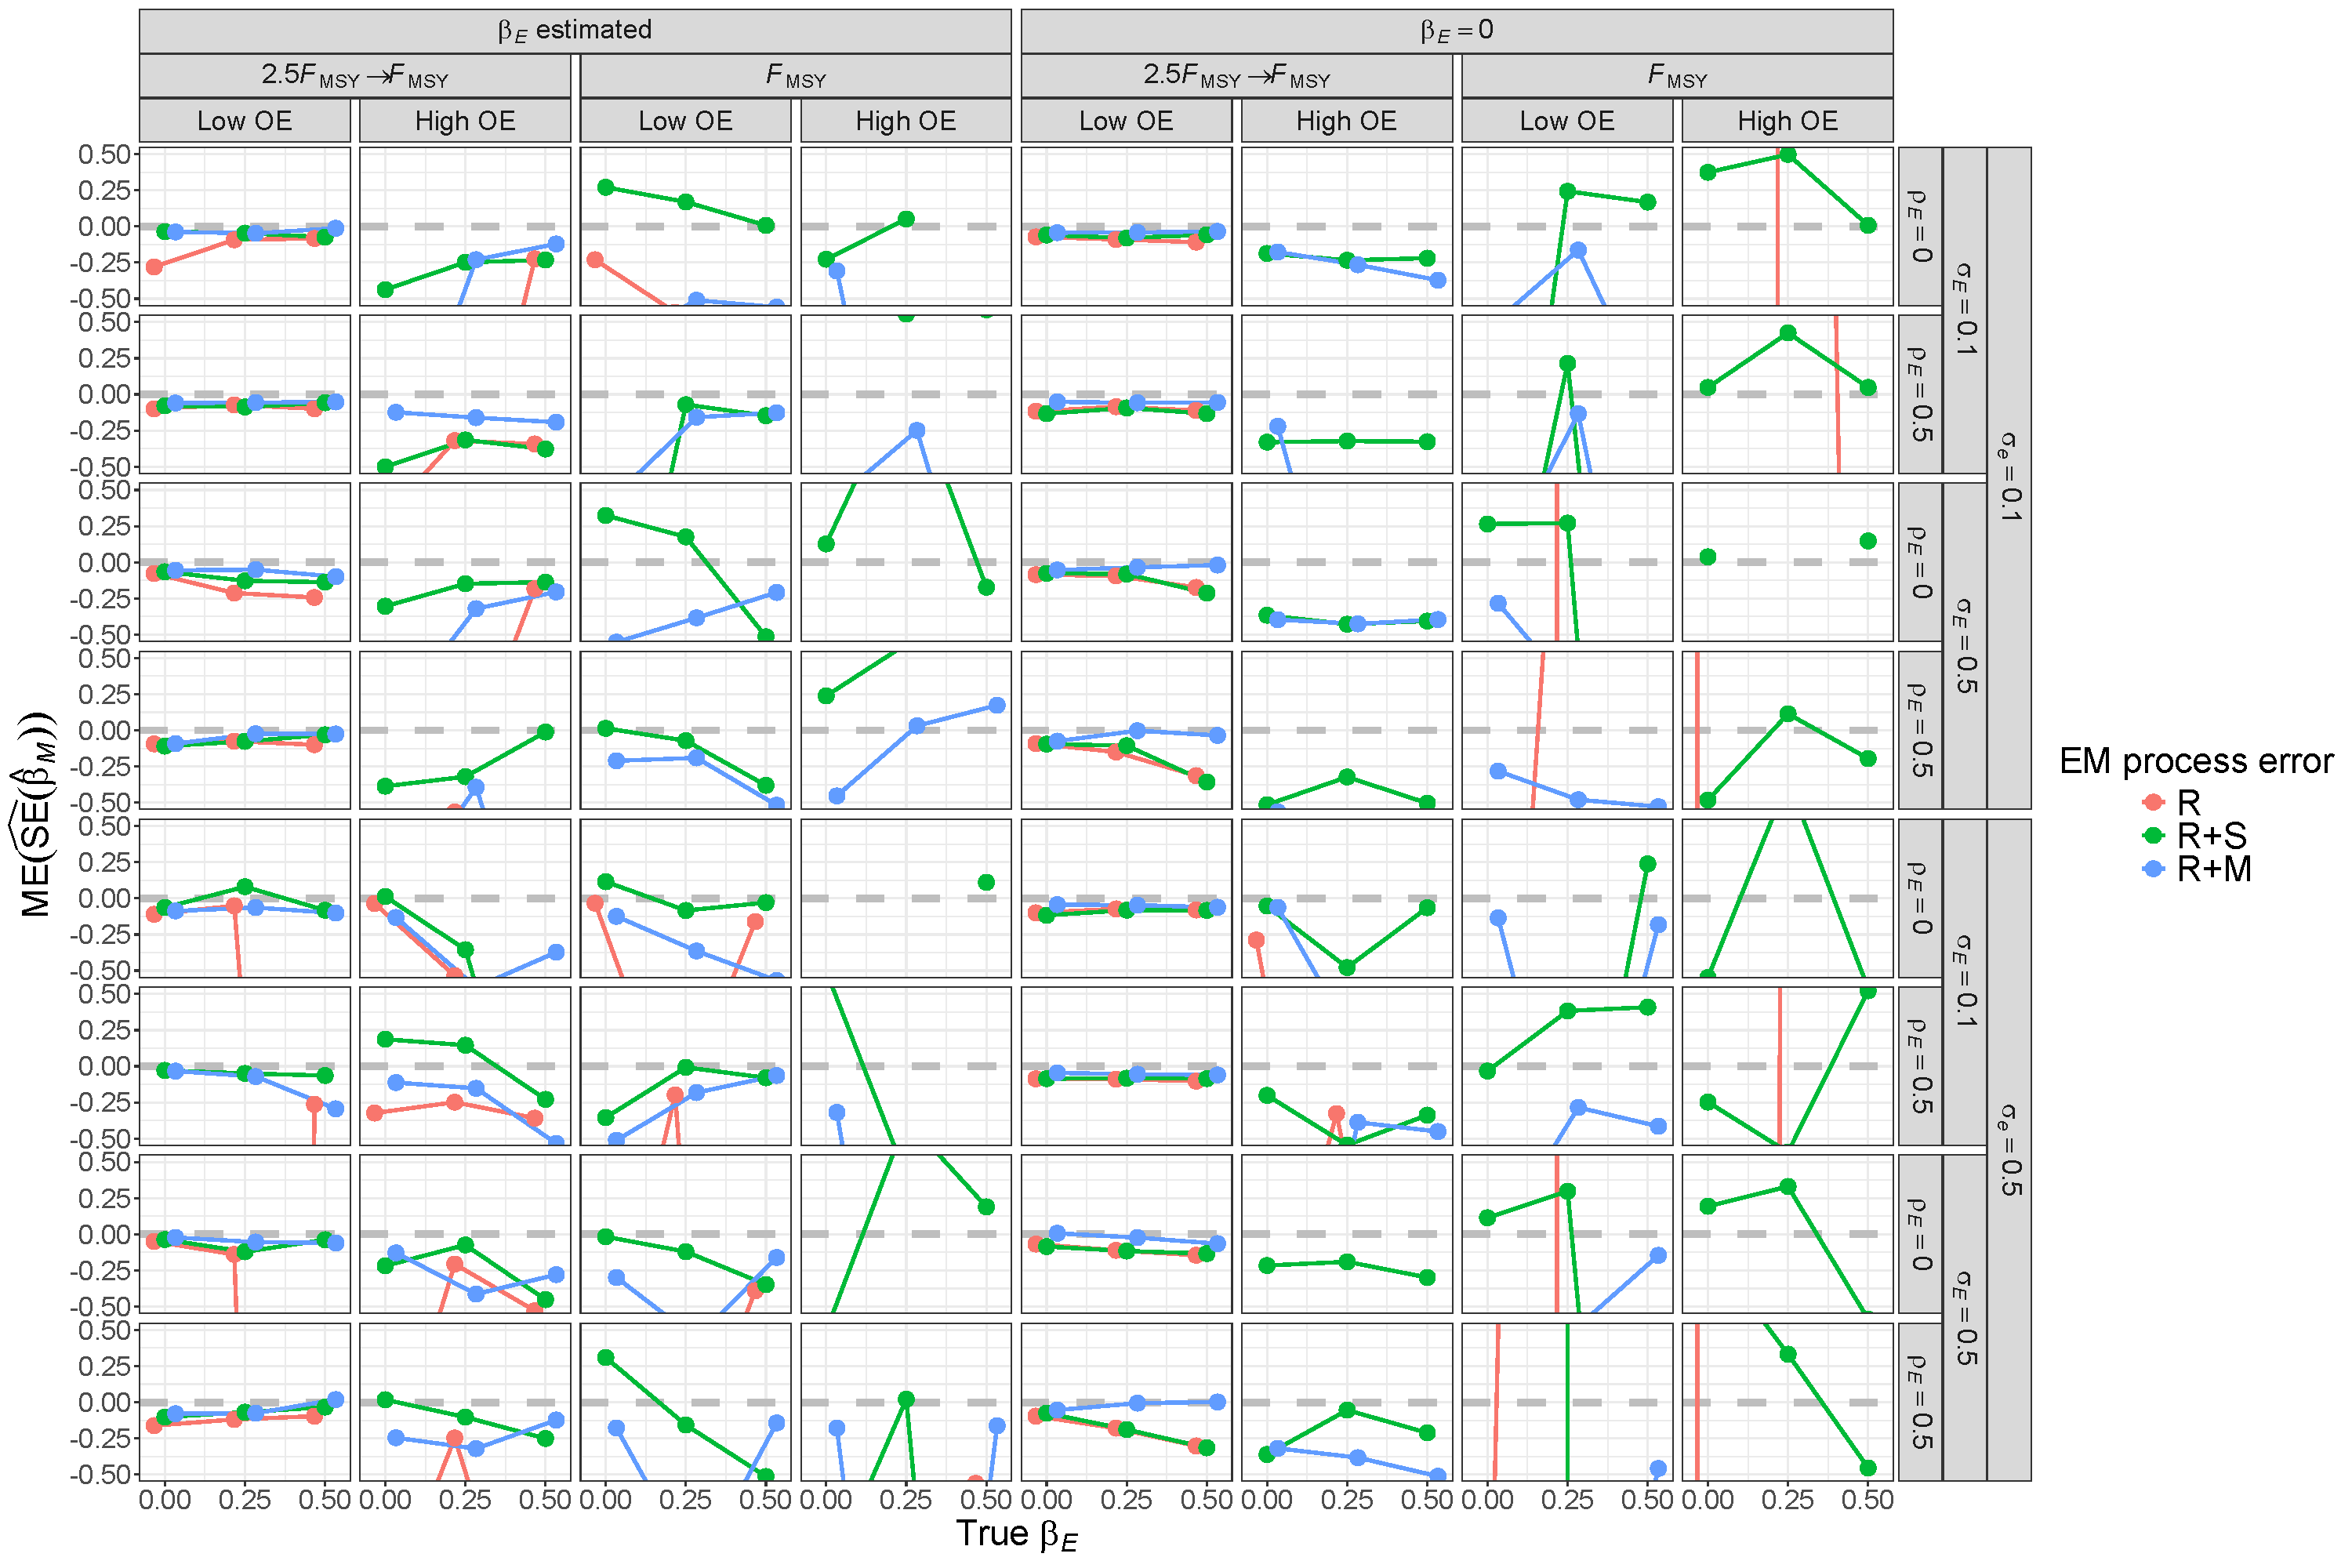
\includegraphics[height = \textheight]{se_beta_M_bias_RMom}
%DIFDELCMD < \end{center}
%DIFDELCMD < %%%
%DIFDELCMD < \caption{%
{%DIFAUXCMD
\DIFdelFL{For R+M OMs, median error (ME) of Hessian-based estimates of standard error for median $M$ parameter ($\beta_M$) from fitting EMs with alternative process error assumptions and treatment of the covariate effect ($\beta_ E= 0$ or estimated). True standard error is defined as the mean of the standard error estimates accross converged fits to simulated data sets for a given OM scenario.}}%DIFAUXCMD
%DIFDELCMD < \label{se_beta_M_bias_RMom}
%DIFDELCMD < \end{figure}
%DIFDELCMD < \end{landscape}
%DIFDELCMD < 

%DIFDELCMD < %%%
\subsection*{\DIFdel{Median Natural mortality parameter confidence interval coverage}}%DIFAUXCMD
%DIFDELCMD < \label{median-natural-mortality-parameter-confidence-interval-coverage}
%DIFDELCMD < %%%
\addcontentsline{toc}{subsection}{\DIFdel{Median Natural mortality parameter confidence interval coverage}}
%DIFAUXCMD
%DIFDELCMD < 

%DIFDELCMD < \begin{landscape}
%DIFDELCMD < \begin{figure}
%DIFDELCMD < \begin{center}
%DIFDELCMD < 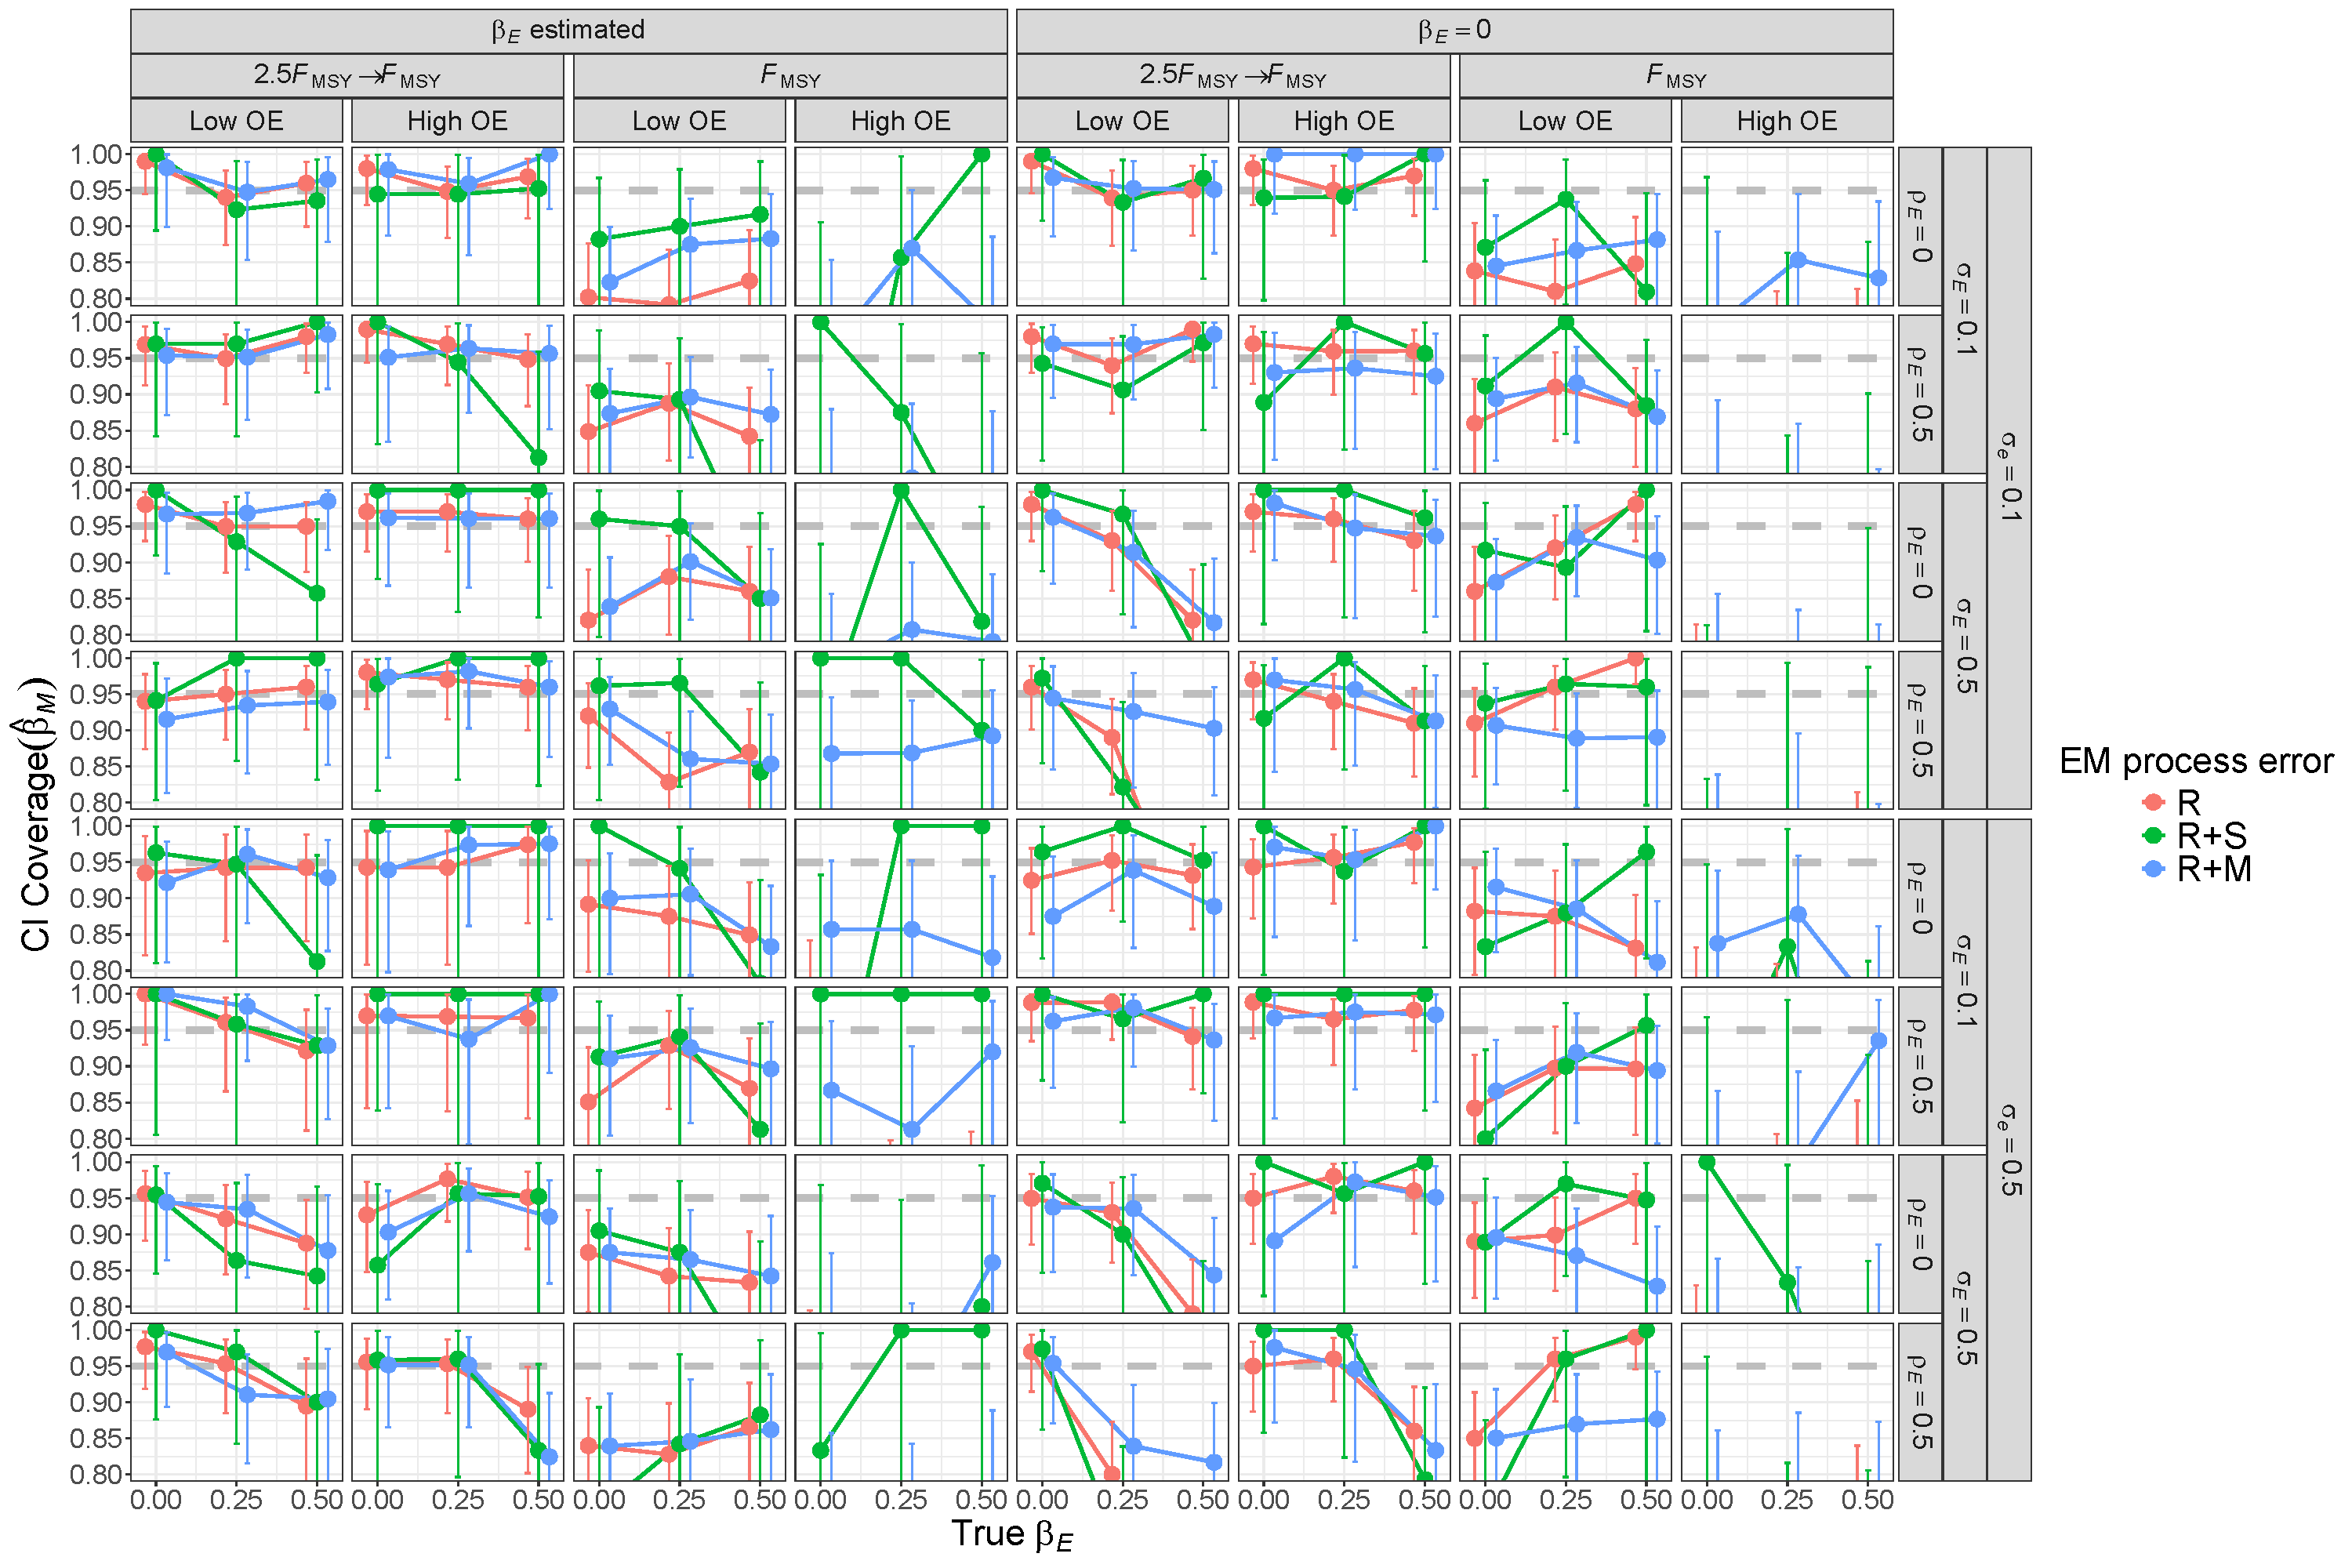
\includegraphics[height = \textheight]{beta_M_CI_coverage_Rom}
%DIFDELCMD < \end{center}
%DIFDELCMD < %%%
%DIFDELCMD < \caption{%
{%DIFAUXCMD
\DIFdelFL{For R OMs, probability of 95\% confidence interval for $\beta_M$ containing the true value for EMs with alternative process error assumptions and treatment of covariate effect ($\beta_E = 0$ or estimated). Vertical lines represent 95\% confidence intervals.}}%DIFAUXCMD
%DIFDELCMD < \label{beta_M_CI_coverage_Rom}
%DIFDELCMD < \end{figure}
%DIFDELCMD < \end{landscape}
%DIFDELCMD < 

%DIFDELCMD < \begin{landscape}
%DIFDELCMD < \begin{figure}
%DIFDELCMD < \begin{center}
%DIFDELCMD < 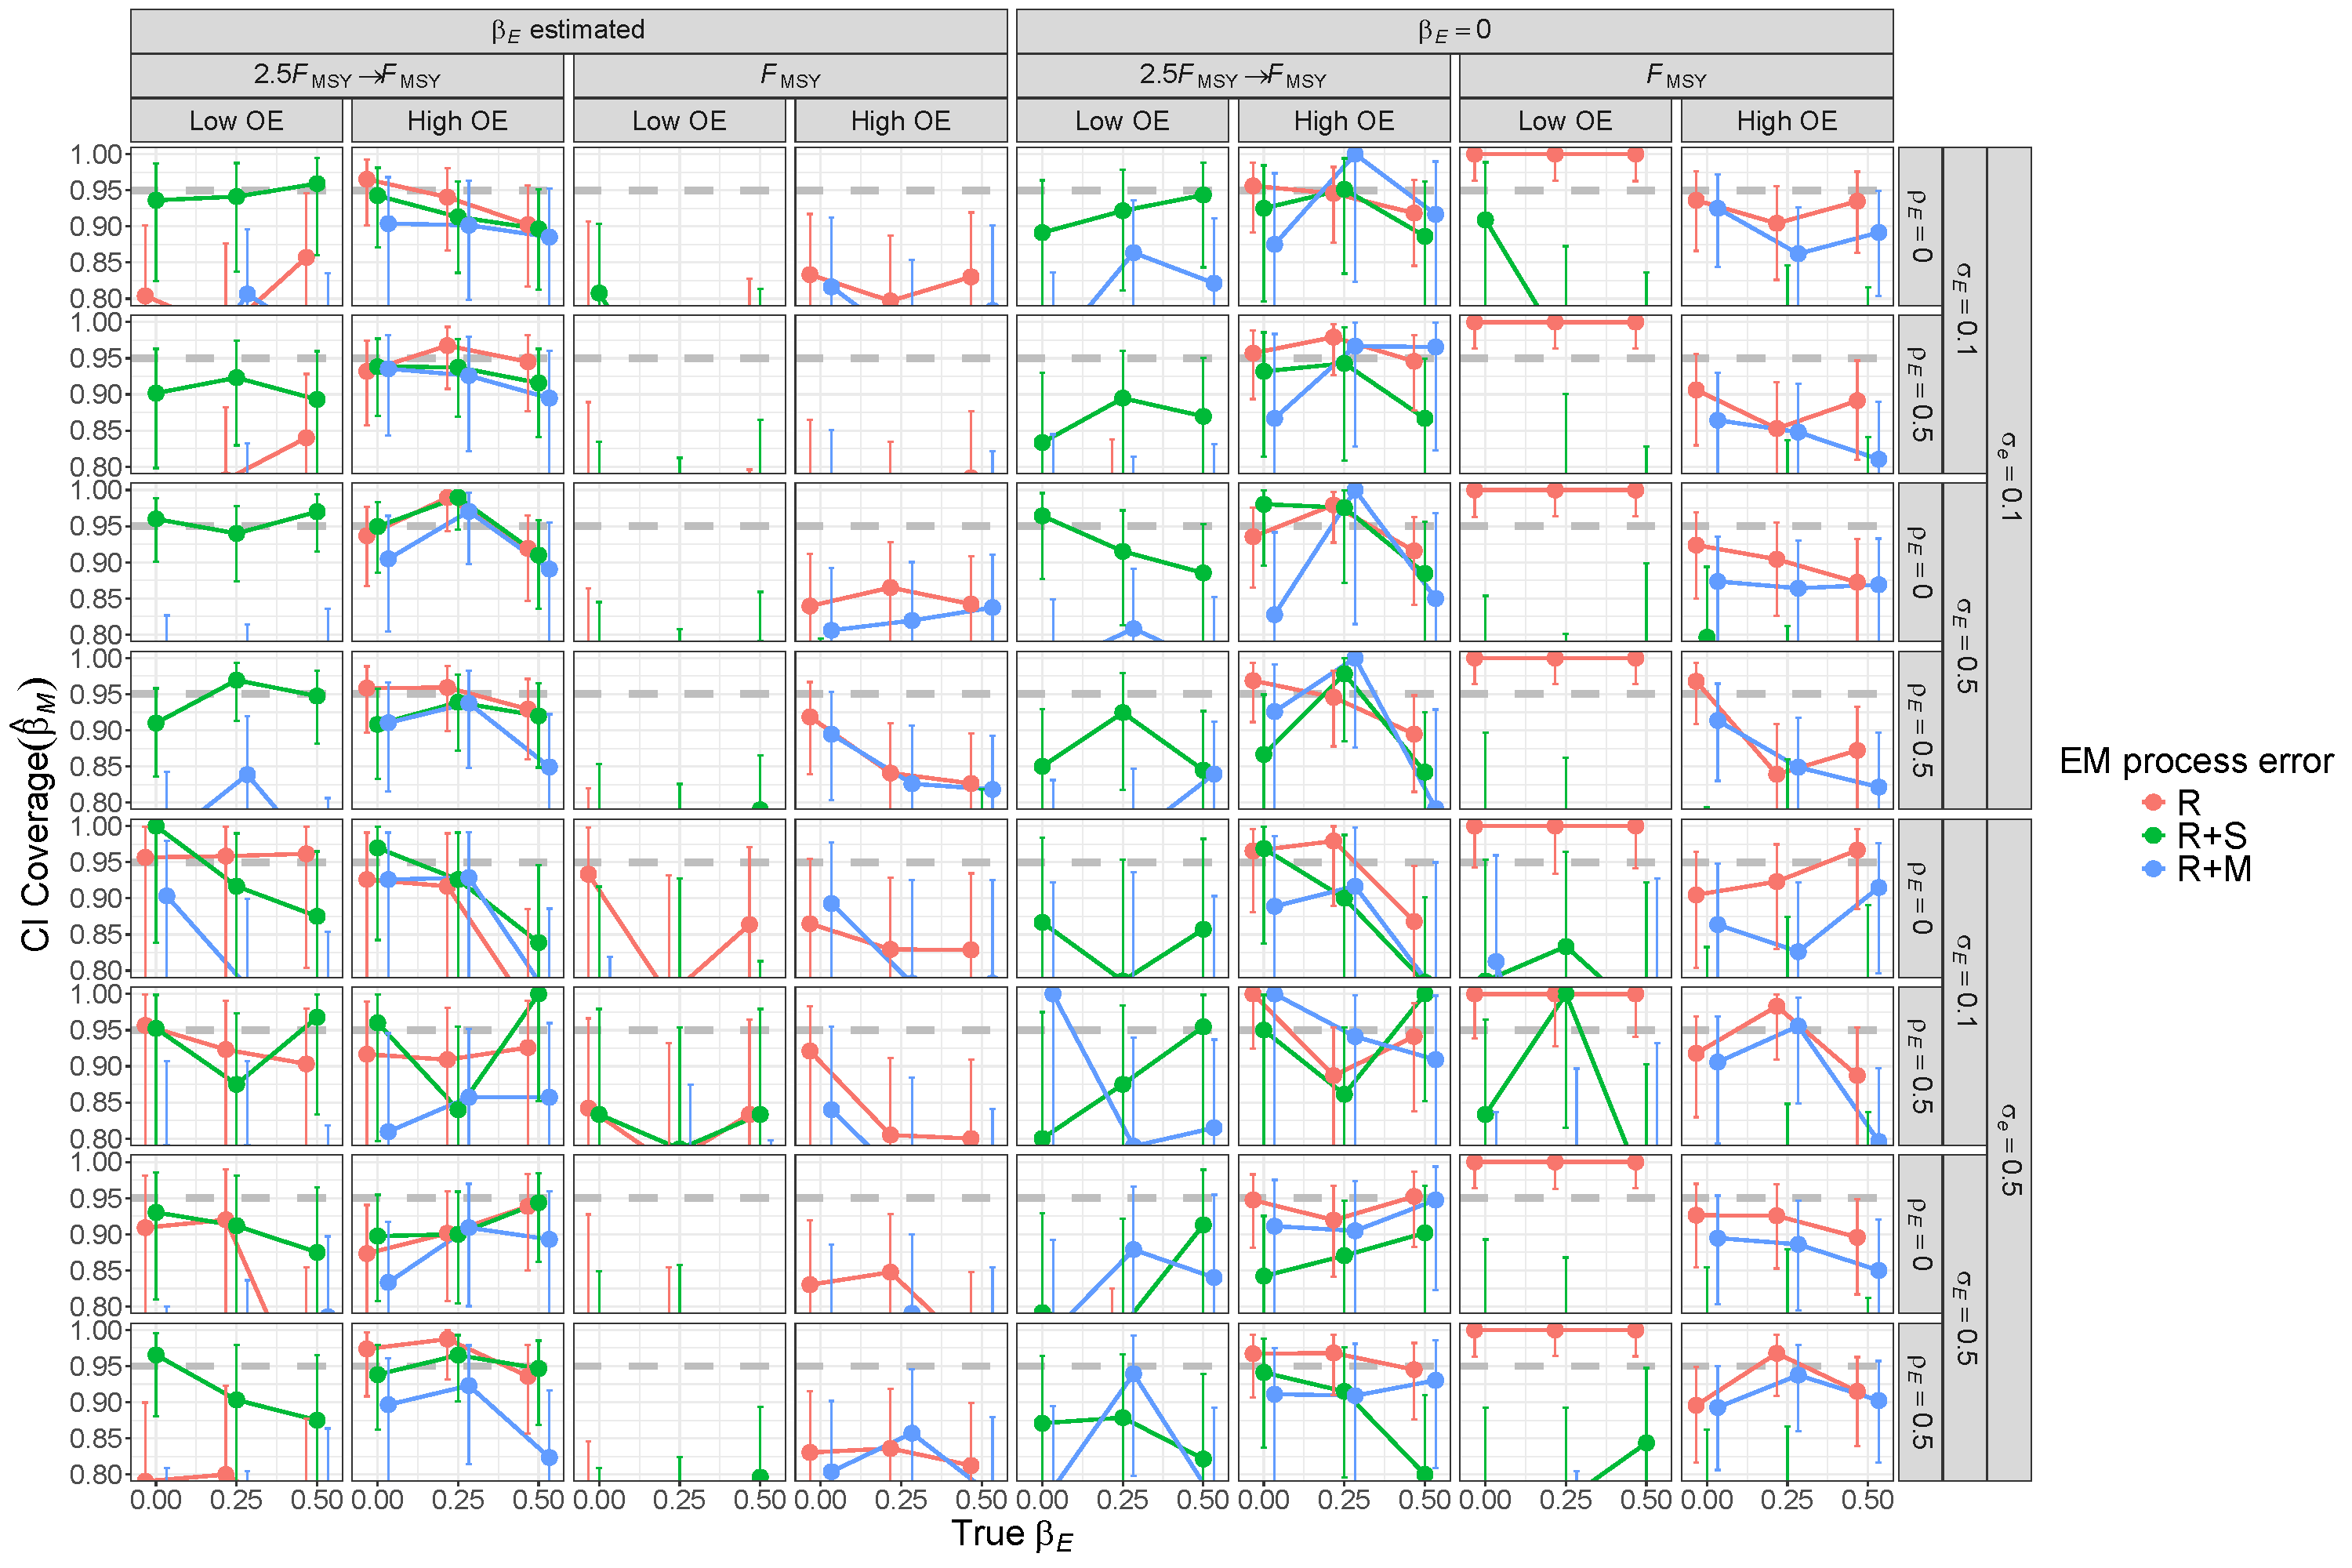
\includegraphics[height = \textheight]{beta_M_CI_coverage_RSom}
%DIFDELCMD < \end{center}
%DIFDELCMD < %%%
%DIFDELCMD < \caption{%
{%DIFAUXCMD
\DIFdelFL{For R+S OMs, probability of 95\% confidence interval for $\beta_M$ containing the true value for EMs with alternative process error assumptions and treatment of covariate effect ($\beta_E = 0$ or estimated). Vertical lines represent 95\% confidence intervals.}}%DIFAUXCMD
%DIFDELCMD < \label{beta_M_CI_coverage_RSom}
%DIFDELCMD < \end{figure}
%DIFDELCMD < \end{landscape}
%DIFDELCMD < 

%DIFDELCMD < \begin{landscape}
%DIFDELCMD < \begin{figure}
%DIFDELCMD < \begin{center}
%DIFDELCMD < 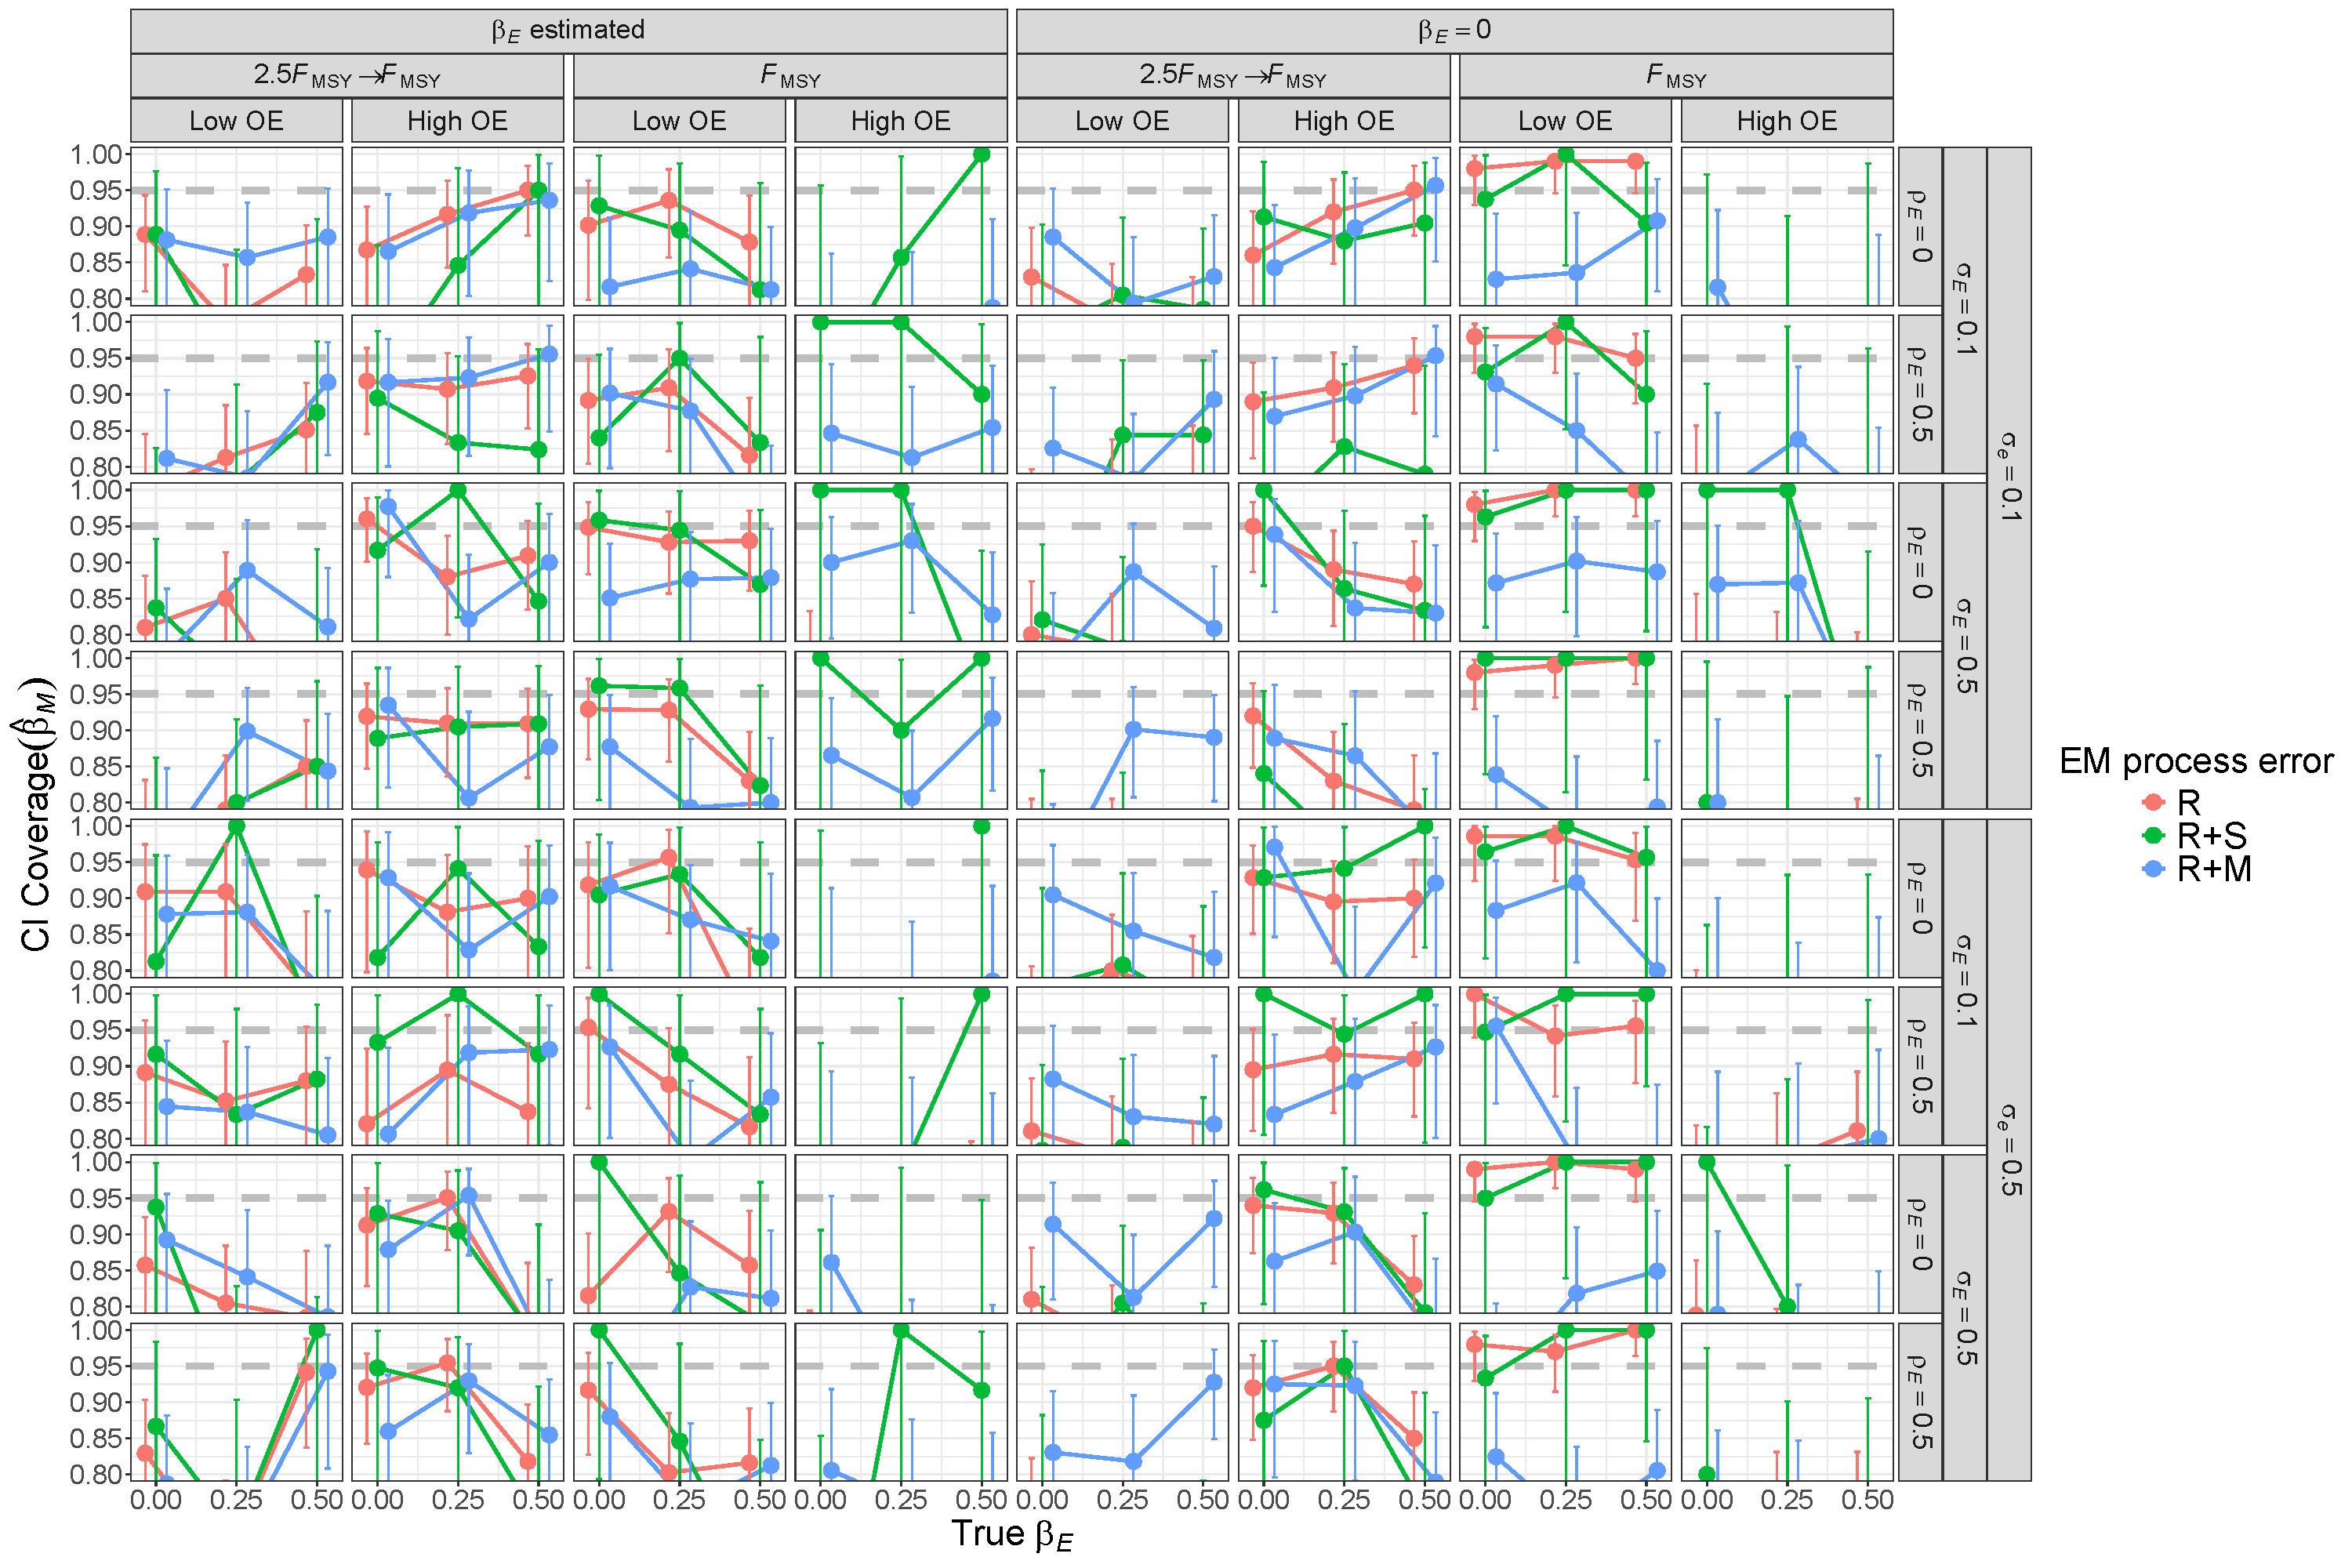
\includegraphics[height = \textheight]{beta_M_CI_coverage_RMom}
%DIFDELCMD < \end{center}
%DIFDELCMD < %%%
%DIFDELCMD < \caption{%
{%DIFAUXCMD
\DIFdelFL{For R+M OMs, probability of 95\% confidence interval for $\beta_M$ containing the true value for EMs with alternative process error assumptions and treatment of covariate effect ($\beta_E = 0$ or estimated). Vertical lines represent 95\% confidence intervals.}}%DIFAUXCMD
%DIFDELCMD < \label{beta_M_CI_coverage_RMom}
%DIFDELCMD < \end{figure}
%DIFDELCMD < \end{landscape}
%DIFDELCMD < 

%DIFDELCMD < %%%
\subsection*{\DIFdel{Median natural mortality parameter estimate and standard error example}}%DIFAUXCMD
%DIFDELCMD < \label{median-natural-mortality-parameter-estimate-and-standard-error-example}
%DIFDELCMD < %%%
\addcontentsline{toc}{subsection}{\DIFdel{Median natural mortality parameter estimate and standard error example}}
%DIFAUXCMD
%DIFDELCMD < 

%DIFDELCMD < \begin{landscape}
%DIFDELCMD < \begin{figure}
%DIFDELCMD < \begin{center}
%DIFDELCMD < 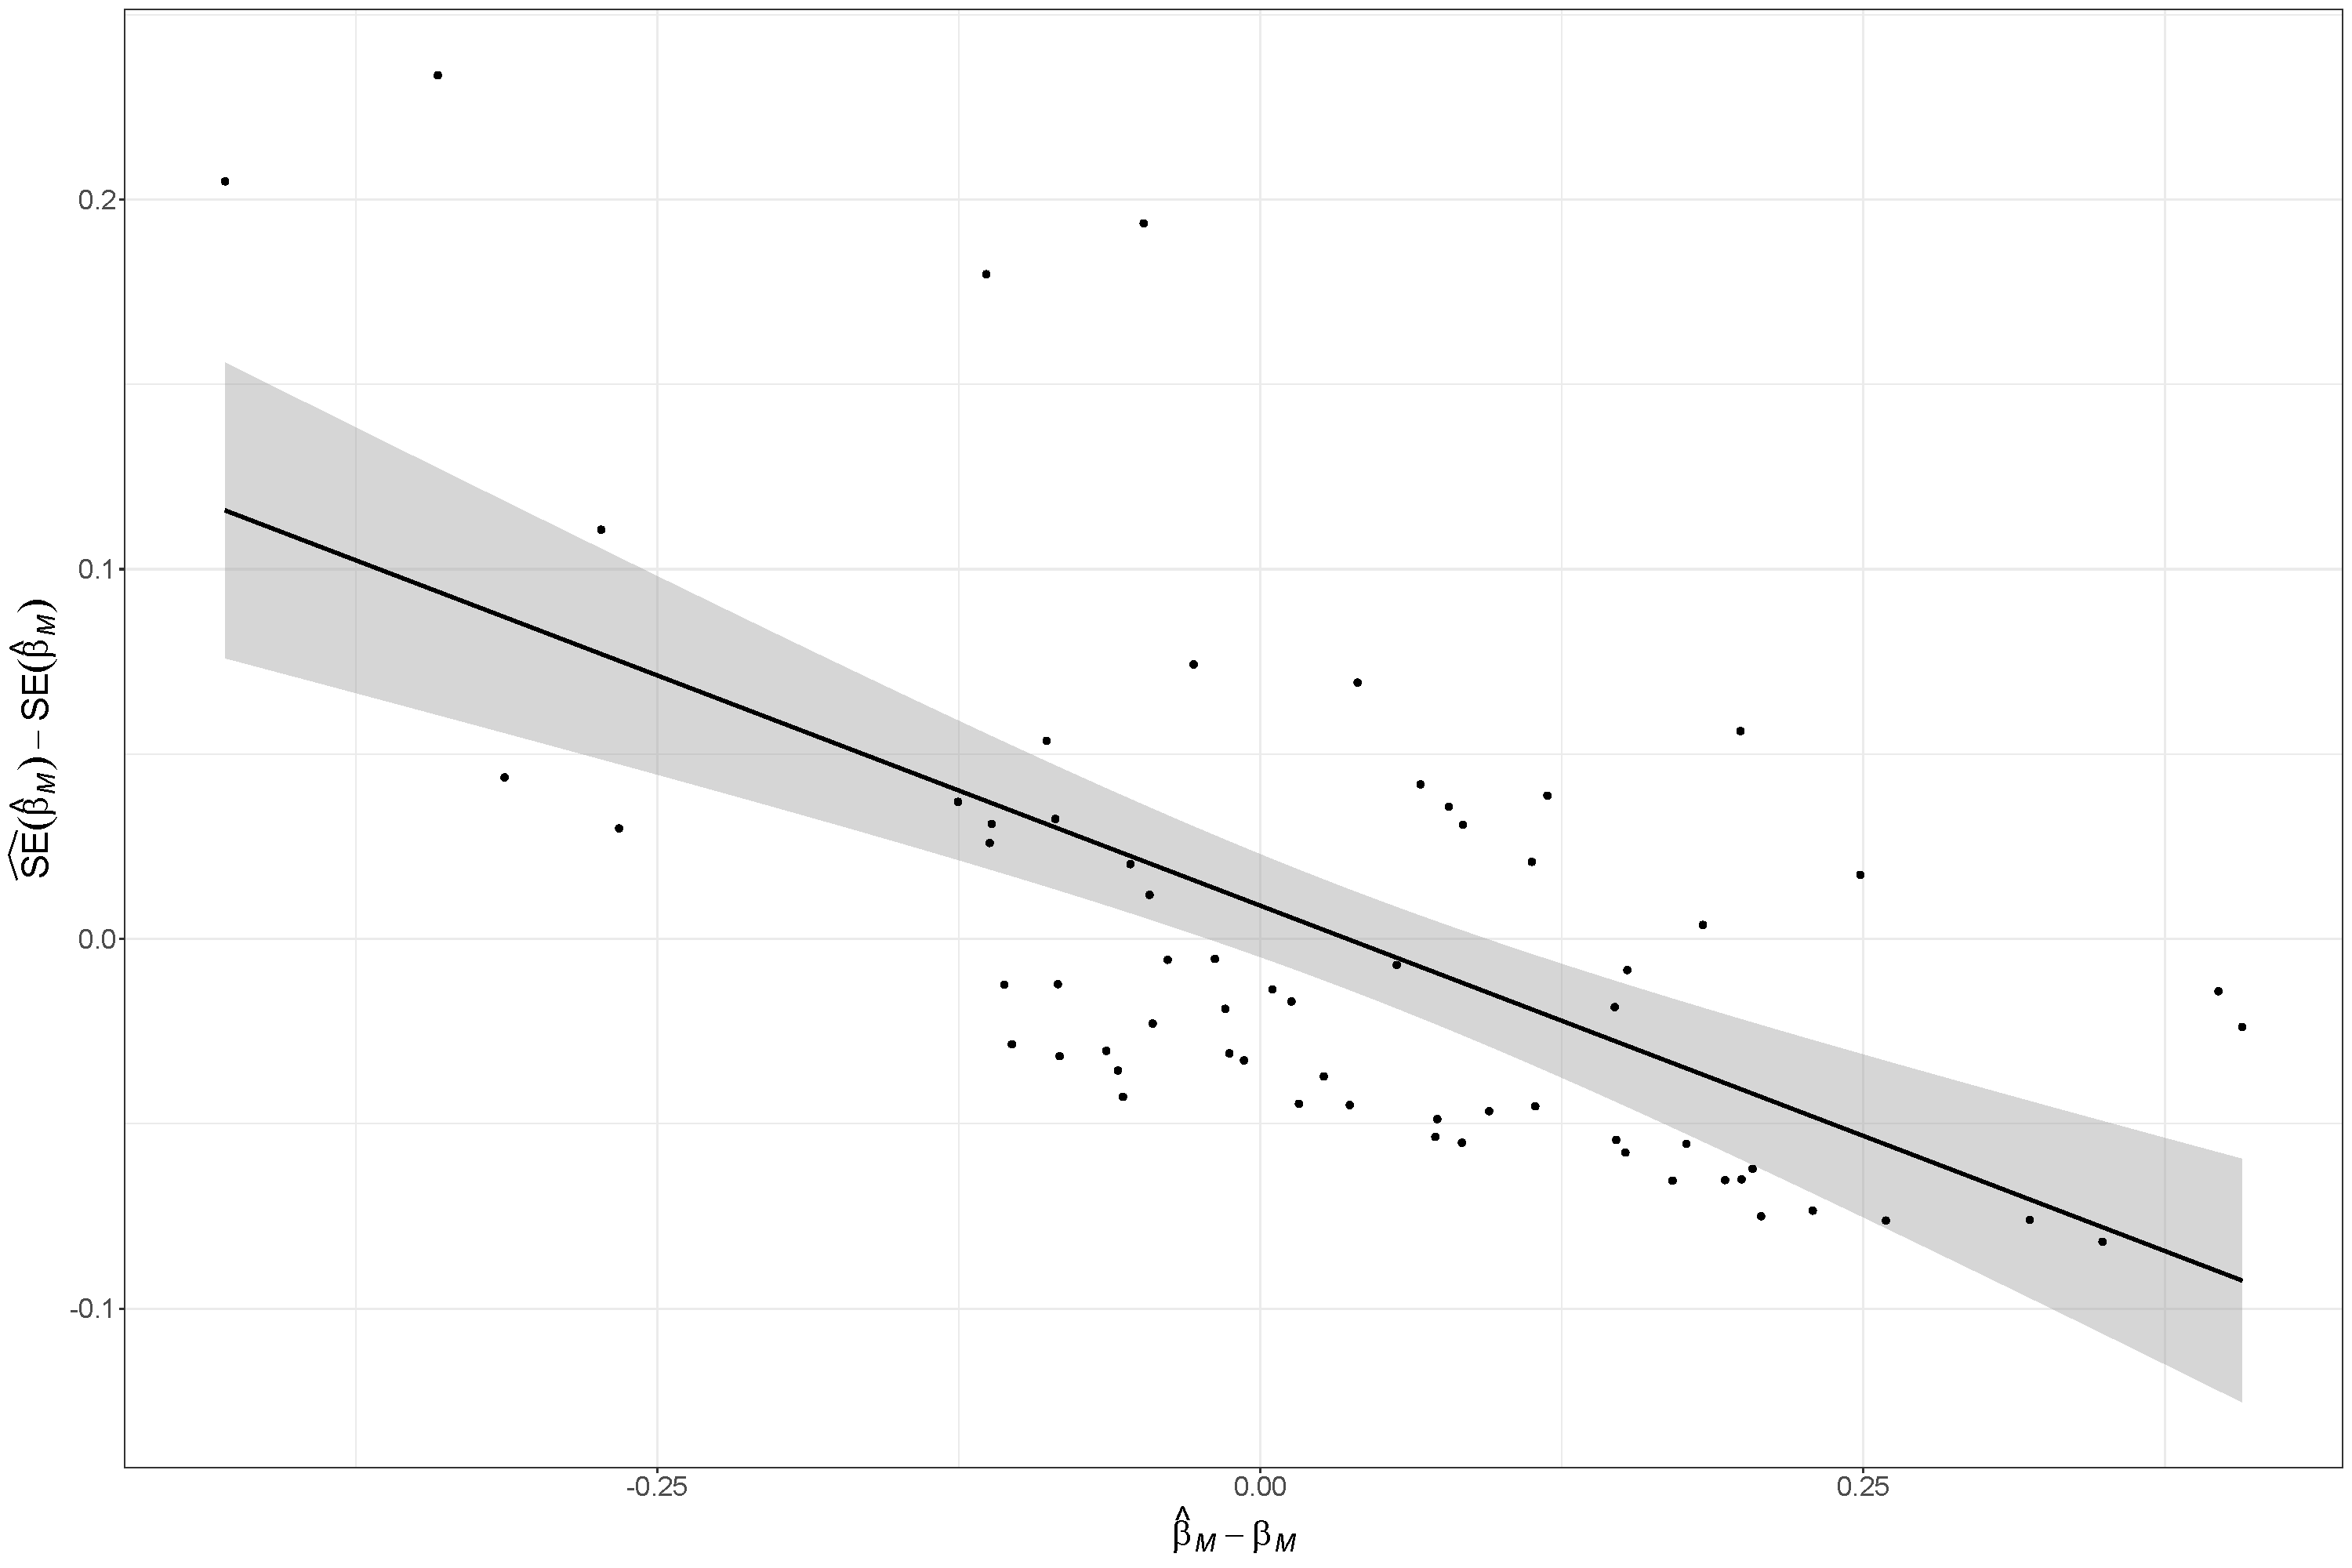
\includegraphics[height = 0.9\textheight]{om_69_em_5_beta_M_se_beta_M_lm_plot}
%DIFDELCMD < \end{center}
%DIFDELCMD < %%%
%DIFDELCMD < \caption{%
{%DIFAUXCMD
\DIFdelFL{Negative correlation of $\beta_M$ estimates and Hessian-based standard error estimates for EM that also estimates the covariate effect and has correct R+M process error assumption fitted to simulated data from the OM with R+M process errors, temporal contrast in fishing pressure, low observation uncertainty for both population ($Low OE$) and covariate observations ($\sigma_e = 0.1$), high and uncorrelated temporal variability in the true covariate ($\sigma_E = 0.5$ and $\rho_E = 0$), and the strongest covariate effect on $M$ ($\beta_E = 0.5$).}}%DIFAUXCMD
%DIFDELCMD < \label{ex_lm_beta_M_SE_beta_M}
%DIFDELCMD < \end{figure}
%DIFDELCMD < \end{landscape}
%DIFDELCMD < 

%DIFDELCMD < %%%
\subsection*{\DIFdel{Median Natural mortality parameter accuracy}}%DIFAUXCMD
%DIFDELCMD < \label{median-natural-mortality-parameter-accuracy}
%DIFDELCMD < %%%
\addcontentsline{toc}{subsection}{\DIFdel{Median Natural mortality parameter accuracy}}
%DIFAUXCMD
%DIFDELCMD < 

%DIFDELCMD < \begin{landscape}
%DIFDELCMD < \begin{figure}
%DIFDELCMD < \begin{center}
%DIFDELCMD < 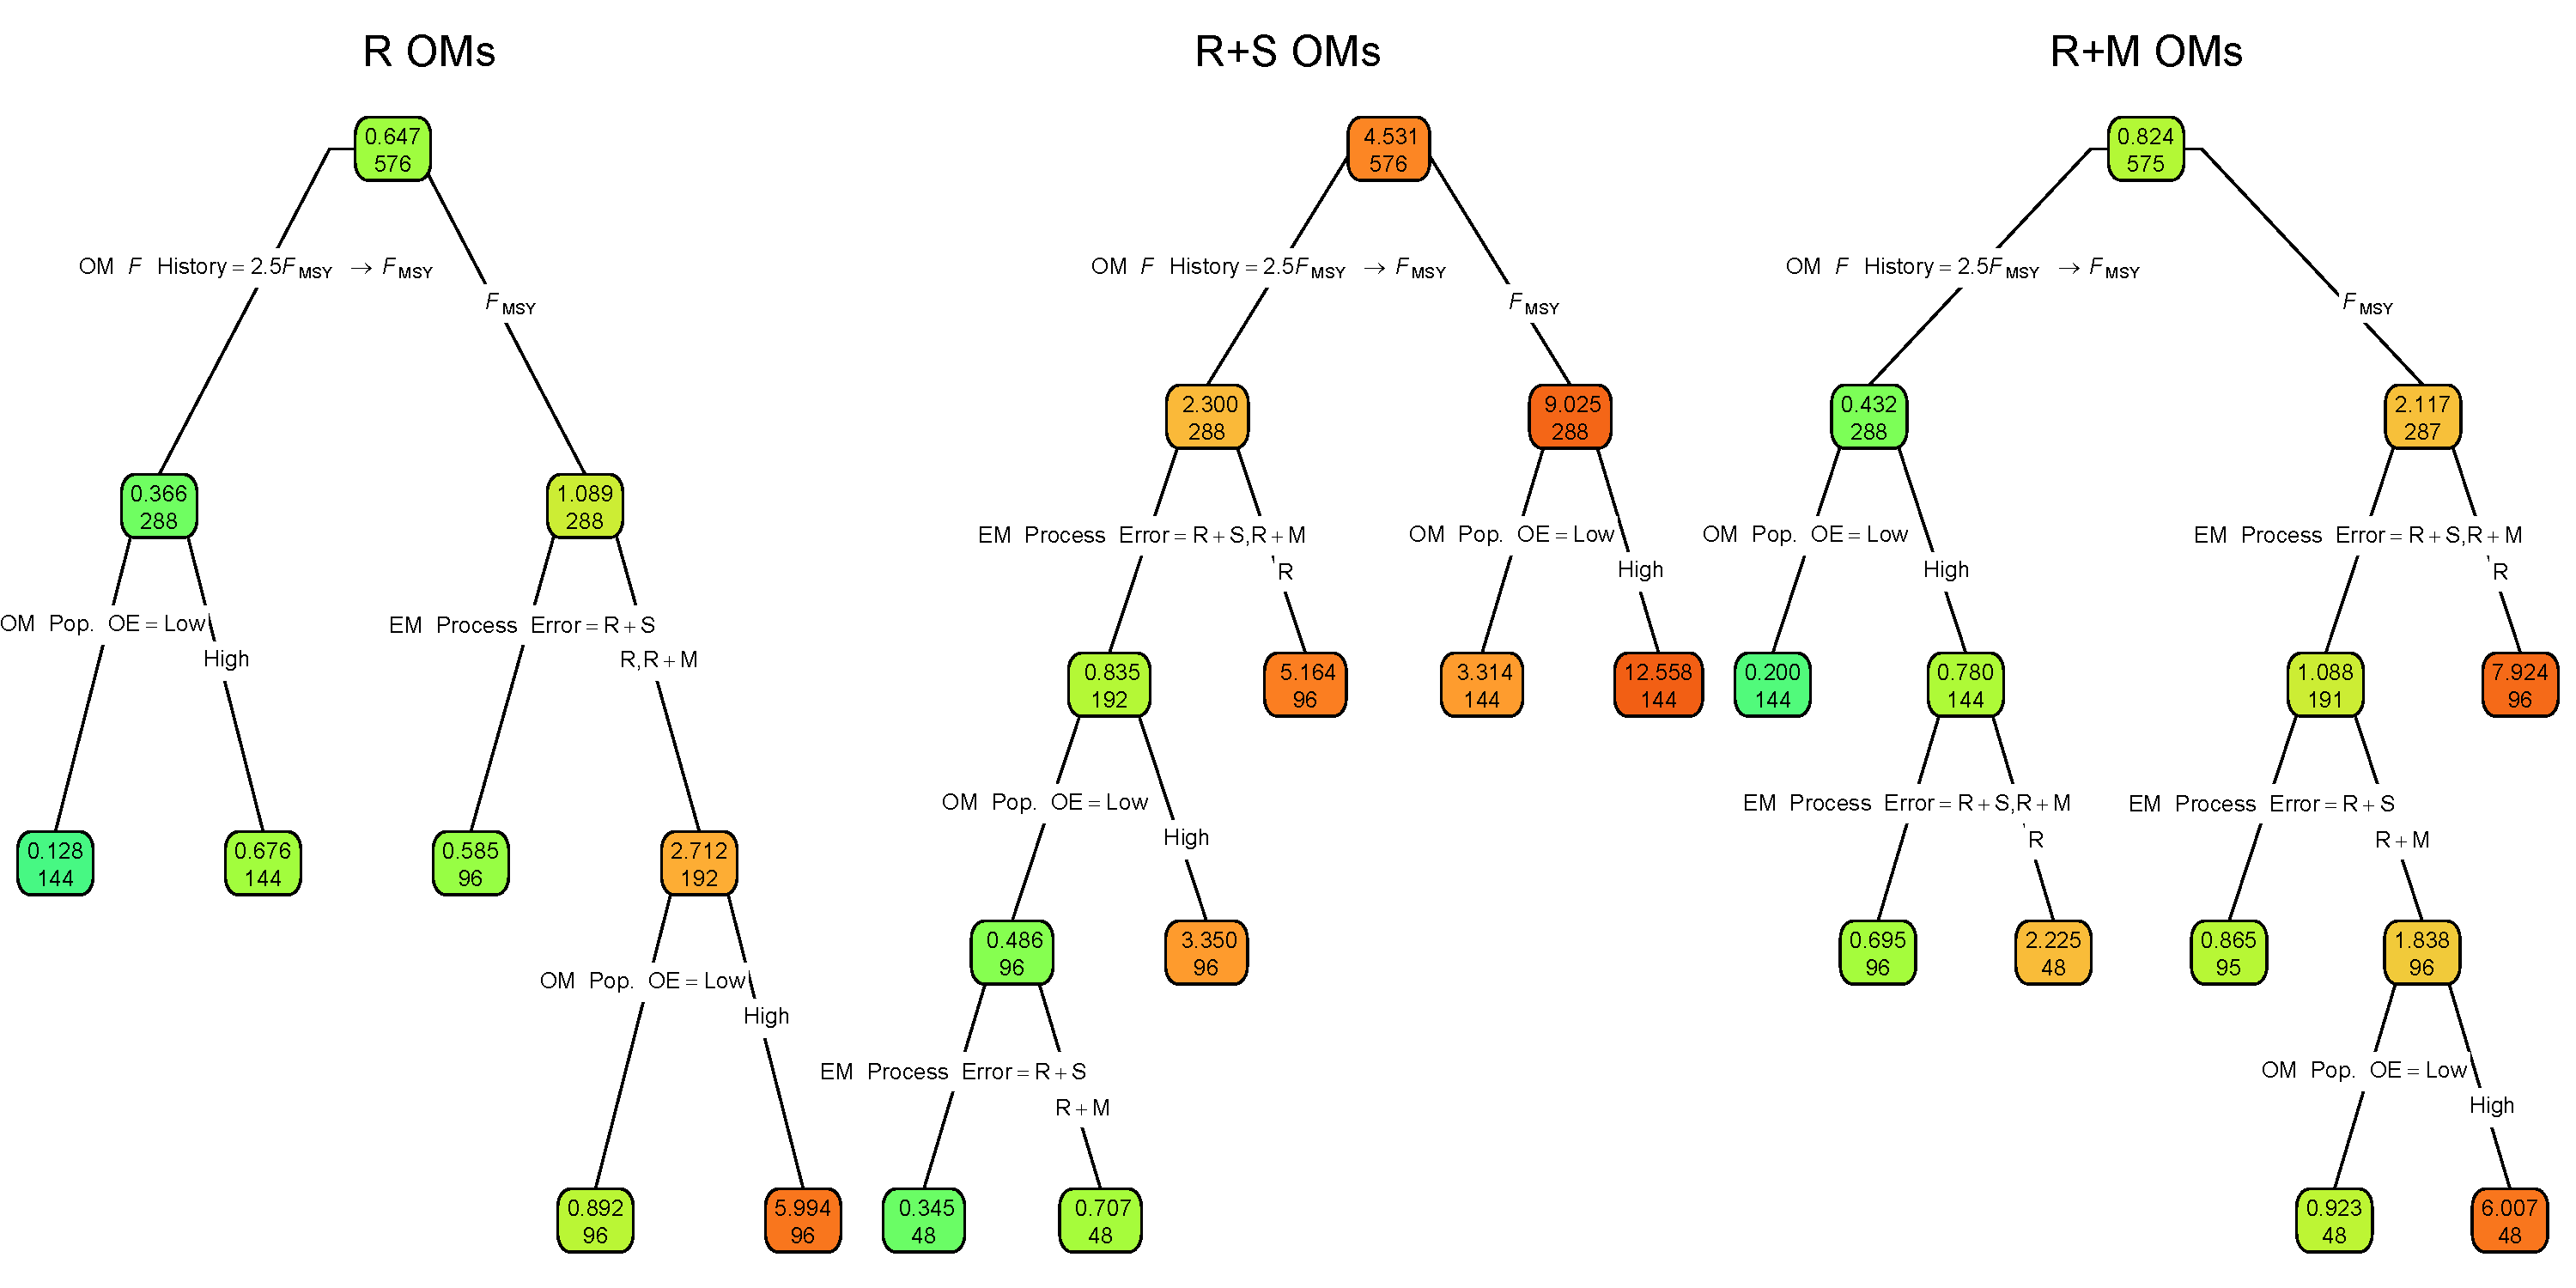
\includegraphics[width = 1.4\textwidth]{median_M_rmse_regtree_plots}
%DIFDELCMD < \end{center}
%DIFDELCMD < %%%
%DIFDELCMD < \caption{%
{%DIFAUXCMD
\DIFdelFL{Regression trees indicating primary factors determining reductions in sums of squares of errors for the log-transformed RMSE of estimates for the median $M$ parameter ($\text{RMSE}\left(\widehat \beta_M\right)$) in EMs fitted to operating models (OMs) with process error on recruitment only (R), recruitment and apparent survival (R+S), or recruitment and natural mortality (R+M). Each node shows the median error (top) and number of observations (bottom) for the corresponding subset. Lower or higher median RMSE are indicated by more green or red polygons, respectively.}}%DIFAUXCMD
%DIFDELCMD < \label{med_M_rmse_regtree}
%DIFDELCMD < \end{figure}
%DIFDELCMD < \end{landscape}
%DIFDELCMD < 

%DIFDELCMD < \begin{table}
%DIFDELCMD < %%%
%DIFDELCMD < \caption{%
{%DIFAUXCMD
\DIFdelFL{Percent reduction in deviance for linear regression models fit to the log-transformed RMSE for estimates of the median $M$ parameter ($\text{RMSE}\left(\widehat \beta_M\right)$). Table rows give each operating model (OM) and estimating model (EM) factor included individually, combined, and with second and third order interactions. Table columns are operating models (OMs) with process error on recruitment only (R), recruitment and apparent survival (R+S), or recruitment and natural mortality (R+M).}}%DIFAUXCMD
%DIFDELCMD < \label{RMSE_mean_M_PRD_table}
%DIFDELCMD < {\begin{center}
%DIFDELCMD < \begin{tabular}{lrrr}
%DIFDELCMD < \hline\hline
%DIFDELCMD < %%%
%DIFDELCMD < \multicolumn{1}{l}{%
{%DIFAUXCMD
\DIFdelFL{Factor}}%DIFAUXCMD
%DIFDELCMD < &%%%
%DIFDELCMD < \multicolumn{1}{c}{%
{%DIFAUXCMD
\DIFdelFL{R}}%DIFAUXCMD
%DIFDELCMD < &%%%
%DIFDELCMD < \multicolumn{1}{c}{%
{%DIFAUXCMD
\DIFdelFL{R+S}}%DIFAUXCMD
%DIFDELCMD < &%%%
%DIFDELCMD < \multicolumn{1}{c}{%
{%DIFAUXCMD
\DIFdelFL{R+M}}%DIFAUXCMD
%DIFDELCMD < \tabularnewline
%DIFDELCMD < \hline
%DIFDELCMD < %%%
\DIFdelFL{OM $F$ history}%DIFDELCMD < &%%%
\DIFdelFL{34.70}%DIFDELCMD < &%%%
\DIFdelFL{24.62}%DIFDELCMD < &%%%
\DIFdelFL{34.91}%DIFDELCMD < \tabularnewline
%DIFDELCMD < %%%
\DIFdelFL{OM Obs. Error}%DIFDELCMD < &%%%
\DIFdelFL{25.55}%DIFDELCMD < &%%%
\DIFdelFL{17.82}%DIFDELCMD < &%%%
\DIFdelFL{12.77}%DIFDELCMD < \tabularnewline
%DIFDELCMD < %%%
\DIFdelFL{$OM \sigma_e$}%DIFDELCMD < & %%%
\DIFdelFL{0.01}%DIFDELCMD < &%%%
\DIFdelFL{\textless  0.01}%DIFDELCMD < &%%%
\DIFdelFL{\textless  0.01}%DIFDELCMD < \tabularnewline
%DIFDELCMD < %%%
\DIFdelFL{$OM \sigma_E$}%DIFDELCMD < & %%%
\DIFdelFL{0.19}%DIFDELCMD < & %%%
\DIFdelFL{0.02}%DIFDELCMD < & %%%
\DIFdelFL{0.07}%DIFDELCMD < \tabularnewline
%DIFDELCMD < %%%
\DIFdelFL{$OM \rho_{E}$}%DIFDELCMD < & %%%
\DIFdelFL{0.05}%DIFDELCMD < & %%%
\DIFdelFL{0.26}%DIFDELCMD < & %%%
\DIFdelFL{0.03}%DIFDELCMD < \tabularnewline
%DIFDELCMD < %%%
\DIFdelFL{OM $\beta_{E}$}%DIFDELCMD < & %%%
\DIFdelFL{0.58}%DIFDELCMD < & %%%
\DIFdelFL{0.23}%DIFDELCMD < & %%%
\DIFdelFL{0.16}%DIFDELCMD < \tabularnewline
%DIFDELCMD < %%%
\DIFdelFL{EM Process Error}%DIFDELCMD < &%%%
\DIFdelFL{10.75}%DIFDELCMD < &%%%
\DIFdelFL{18.12}%DIFDELCMD < &%%%
\DIFdelFL{14.50}%DIFDELCMD < \tabularnewline
%DIFDELCMD < %%%
\DIFdelFL{$EM \beta_{E}$ }\DIFdelendFL \DIFaddbeginFL \DIFaddFL{EM $M$ }\DIFaddendFL assumption&\DIFdelbeginFL \DIFdelFL{3.96}\DIFdelendFL \DIFaddbeginFL \DIFaddFL{28.94}\DIFaddendFL &\DIFdelbeginFL \DIFdelFL{6.39}\DIFdelendFL \DIFaddbeginFL \DIFaddFL{19.74}\DIFaddendFL &\DIFdelbeginFL \DIFdelFL{2.93}\DIFdelendFL \DIFaddbeginFL \DIFaddFL{25.36}\DIFaddendFL \tabularnewline
All factors&\DIFdelbeginFL \DIFdelFL{75.79}\DIFdelendFL \DIFaddbeginFL \DIFaddFL{61.19}\DIFaddendFL &\DIFdelbeginFL \DIFdelFL{67.47}\DIFdelendFL \DIFaddbeginFL \DIFaddFL{52.21}\DIFaddendFL &\DIFdelbeginFL \DIFdelFL{65.26}\DIFdelendFL \DIFaddbeginFL \DIFaddFL{56.09}\DIFaddendFL \tabularnewline
+ All Two Way&\DIFdelbeginFL \DIFdelFL{90.21}\DIFdelendFL \DIFaddbeginFL \DIFaddFL{81.48}\DIFaddendFL &\DIFdelbeginFL \DIFdelFL{80.65}\DIFdelendFL \DIFaddbeginFL \DIFaddFL{72.16}\DIFaddendFL &\DIFdelbeginFL \DIFdelFL{77.59}\DIFdelendFL \DIFaddbeginFL \DIFaddFL{74.98}\DIFaddendFL \tabularnewline
+ All Three Way&\DIFdelbeginFL \DIFdelFL{93.72}\DIFdelendFL \DIFaddbeginFL \DIFaddFL{85.23}\DIFaddendFL &\DIFdelbeginFL \DIFdelFL{88.68}\DIFdelendFL \DIFaddbeginFL \DIFaddFL{83.22}\DIFaddendFL &\DIFdelbeginFL \DIFdelFL{86.44}\DIFdelendFL \DIFaddbeginFL \DIFaddFL{80.48}\DIFaddendFL \tabularnewline
\hline
\end{tabular}\end{center}
}
\end{table}
\DIFaddbegin \pagebreak
\DIFaddend 

\DIFaddbegin \subsection*{\DIFadd{Further detailed results}}\label{further-detailed-results}
\addcontentsline{toc}{subsection}{\DIFadd{Further detailed results}}

\DIFaddend \begin{landscape}
\begin{figure}
\begin{center}
\DIFdelbeginFL %DIFDELCMD < 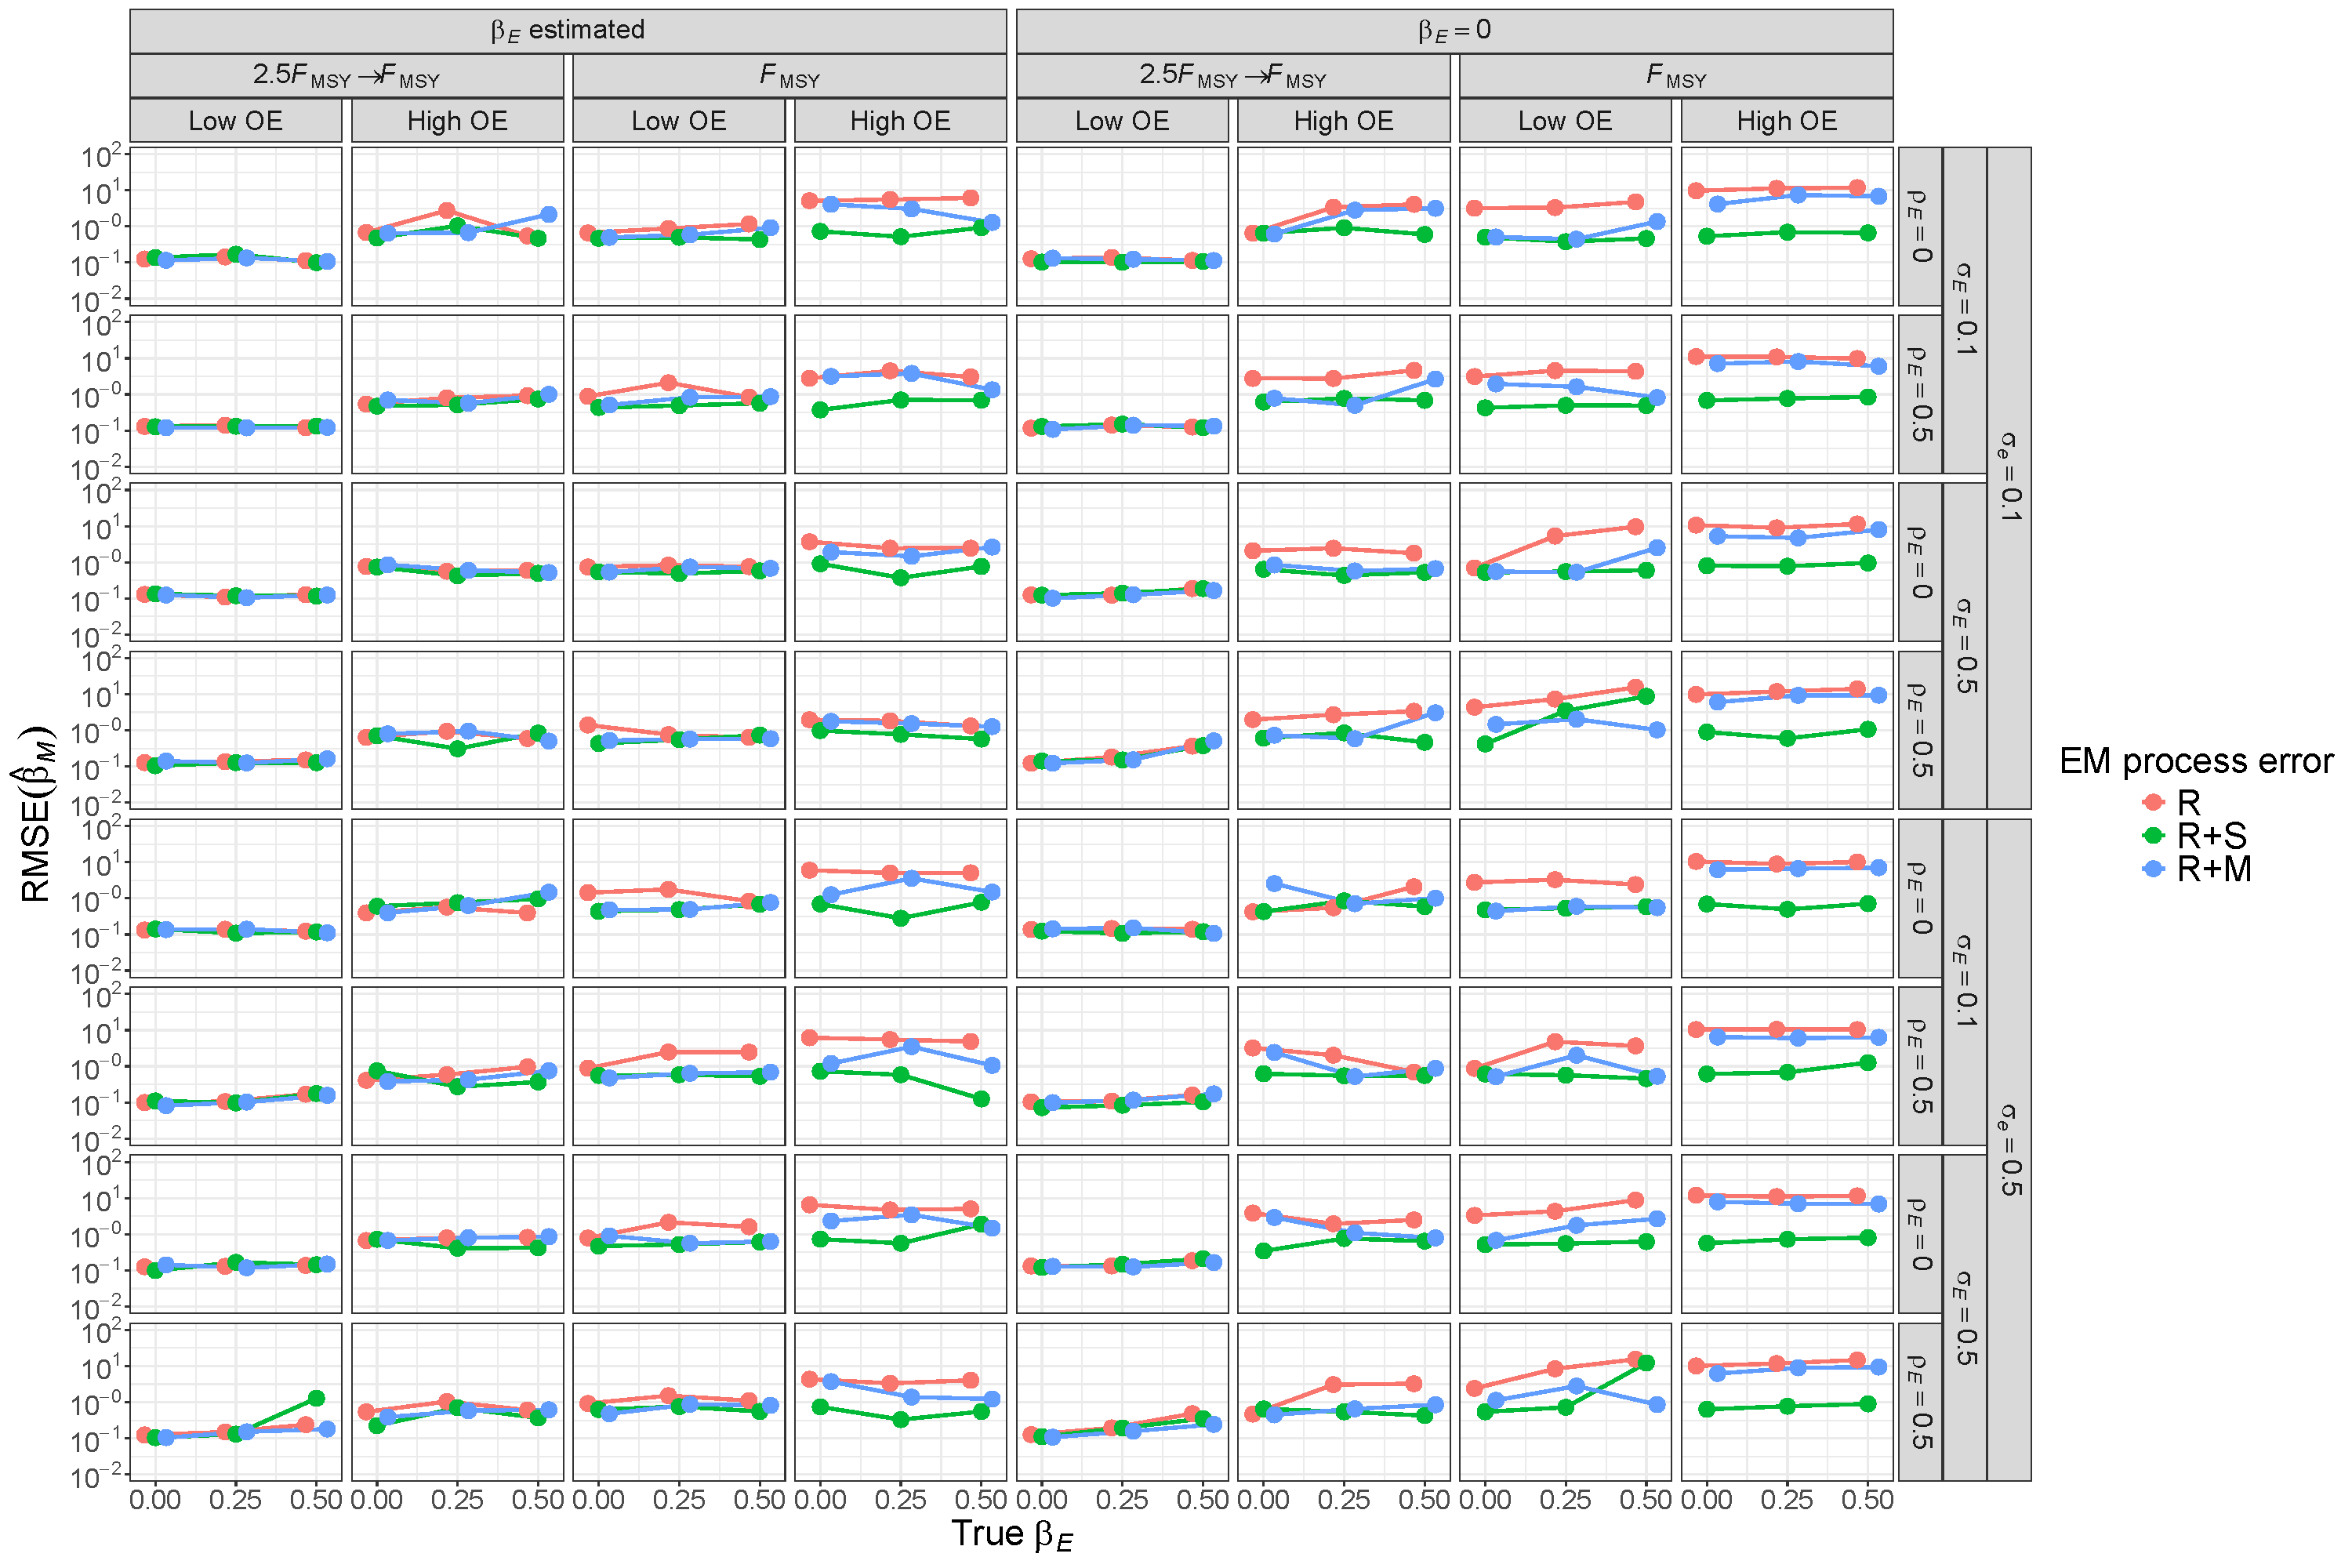
\includegraphics[height = \textheight]{beta_M_rmse_Rom}
%DIFDELCMD < %%%
\DIFdelendFL \DIFaddbeginFL 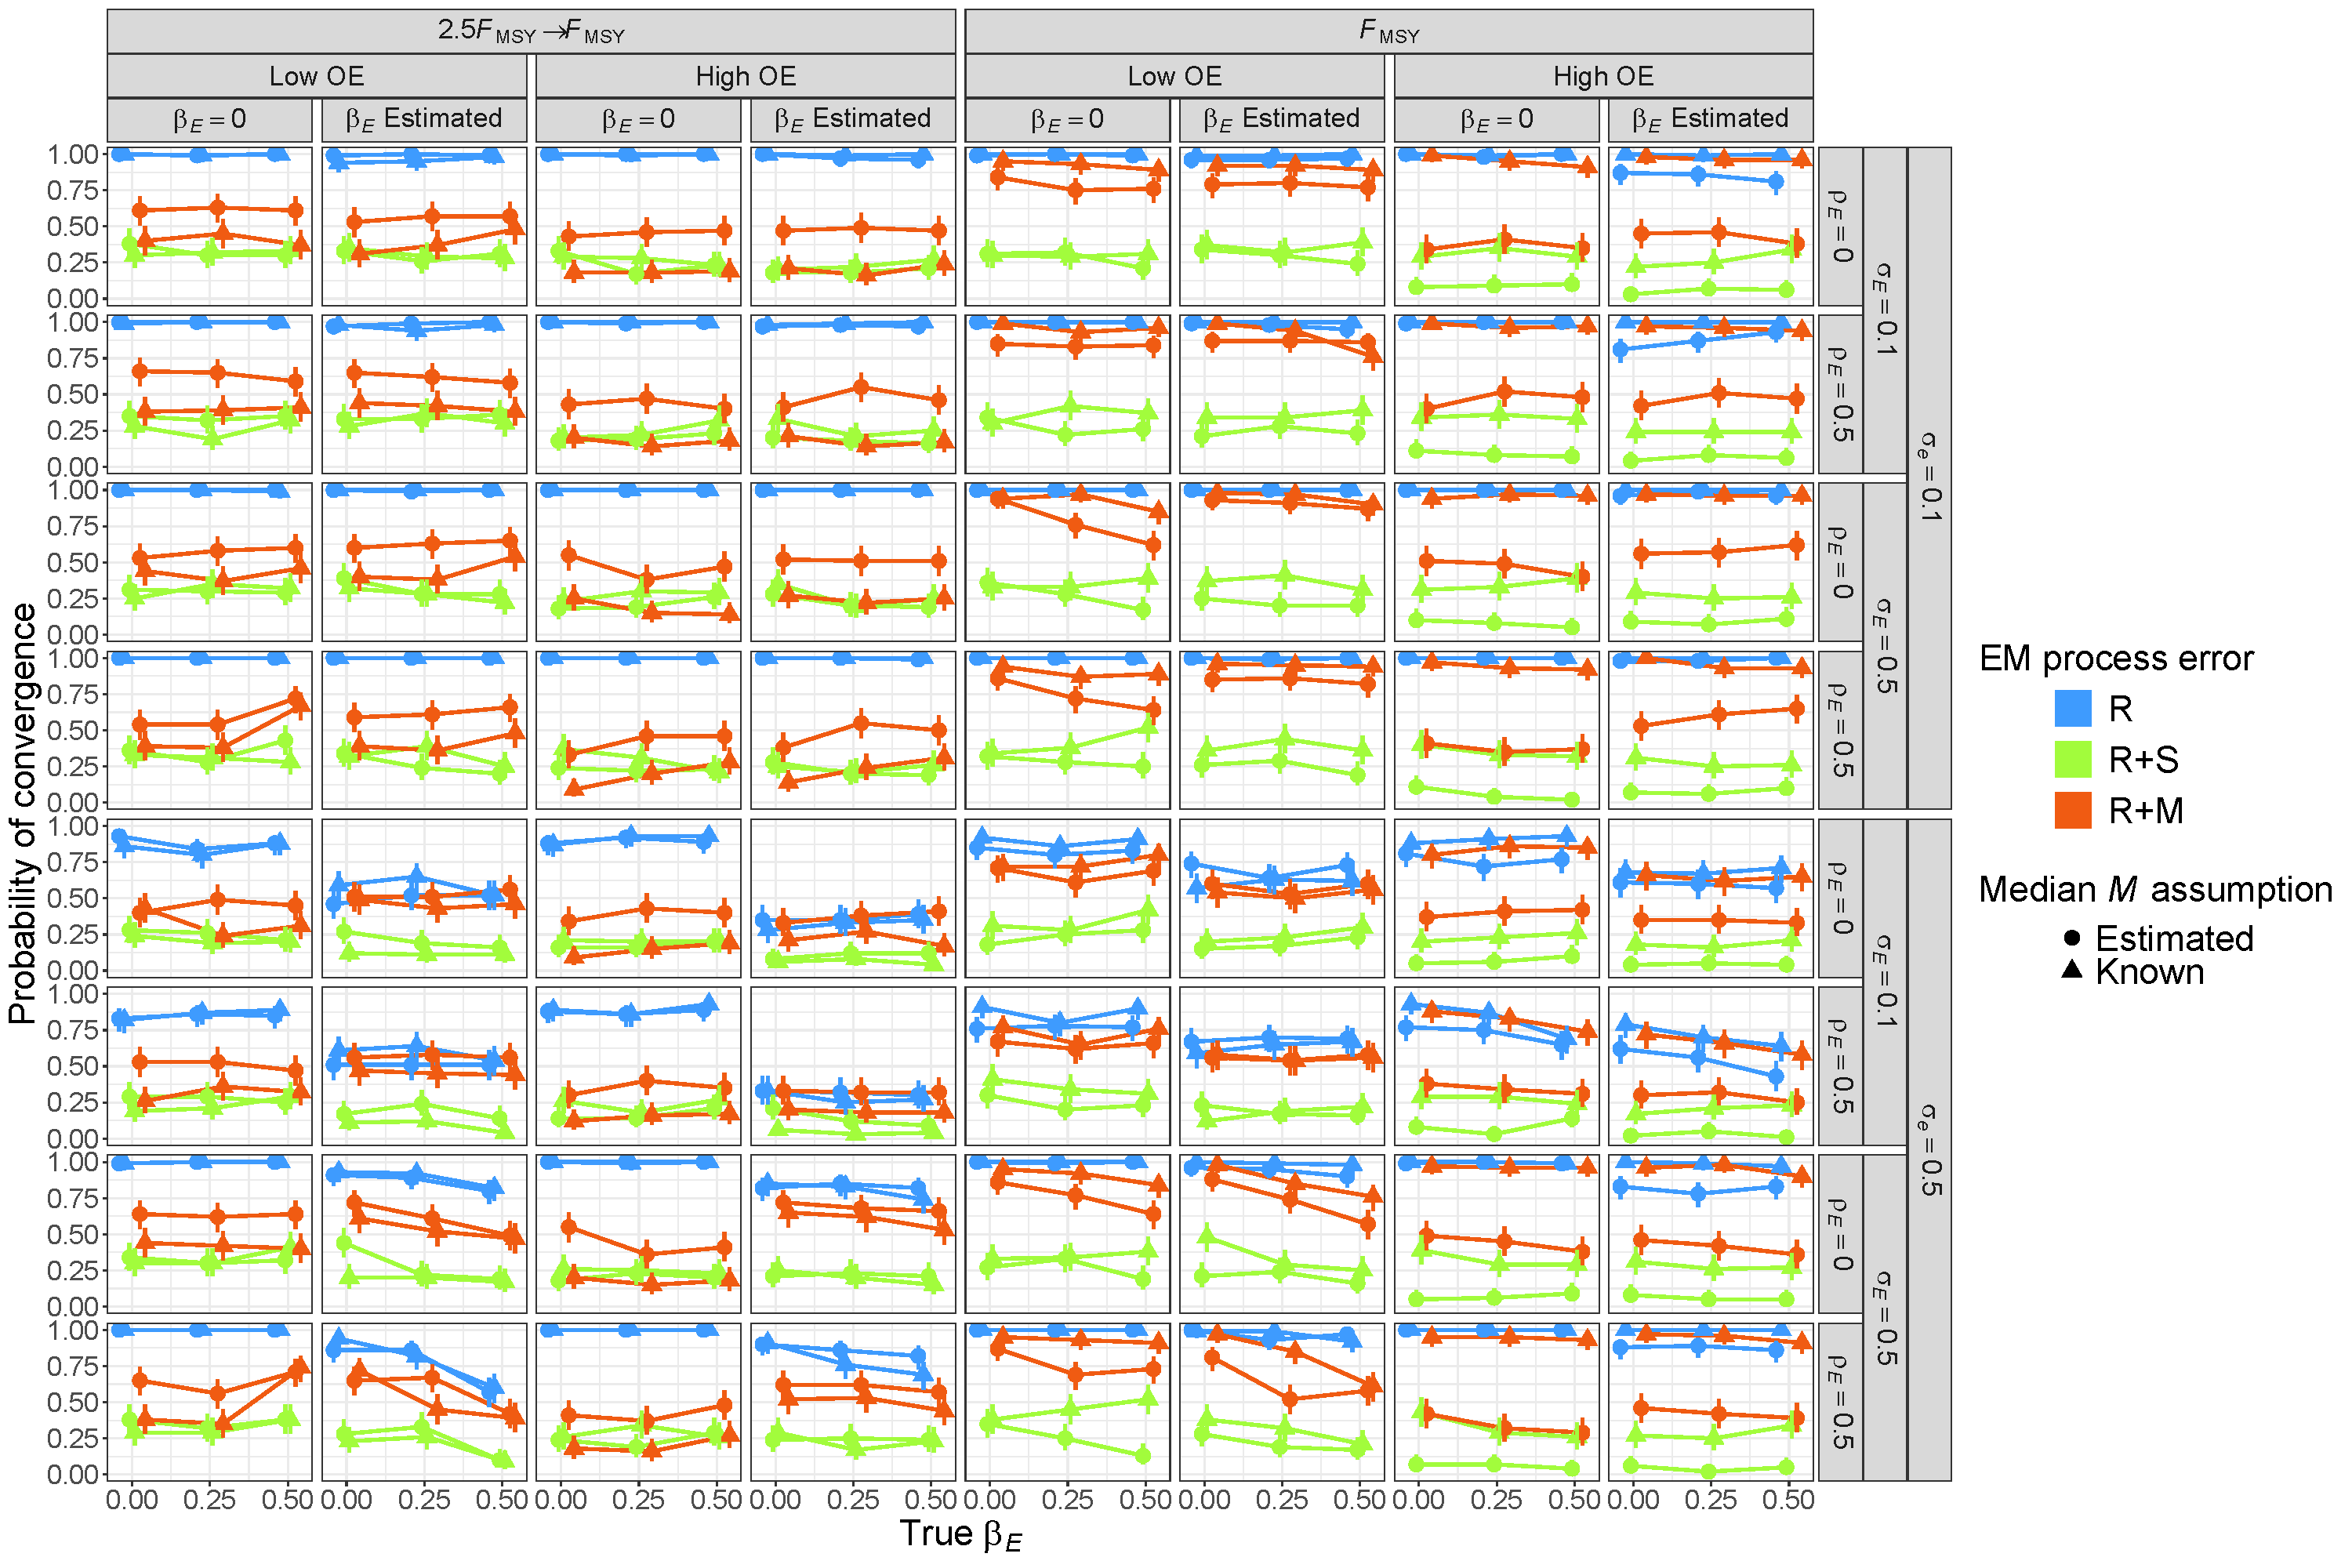
\includegraphics[height = \textheight]{convergence_Rom}
\DIFaddendFL \end{center}
\caption{\DIFdelbeginFL \DIFdelFL{For R OMs, RMSE }\DIFdelendFL \DIFaddbeginFL \DIFaddFL{Estimated probability }\DIFaddendFL of \DIFdelbeginFL \DIFdelFL{estimates of  $\beta_M$ from fitting EMs with }\DIFdelendFL \DIFaddbeginFL \DIFaddFL{fits providing Hessian-based standard errors for estimating models assuming }\DIFaddendFL alternative process error\DIFdelbeginFL \DIFdelFL{assumptions }\DIFdelendFL \DIFaddbeginFL \DIFaddFL{, that estimate or assume known median $M$, }\DIFaddendFL and \DIFdelbeginFL \DIFdelFL{treatment }\DIFdelendFL \DIFaddbeginFL \DIFaddFL{that estimate or assume no covariate effect on median $M$ when fitted to R operating models and three levels }\DIFaddendFL of \DIFaddbeginFL \DIFaddFL{true }\DIFaddendFL covariate effect \DIFaddbeginFL \DIFaddFL{on median $M$ }\DIFaddendFL (\DIFdelbeginFL \DIFdelFL{$\beta_E = 0$ or estimated}\DIFdelendFL \DIFaddbeginFL \DIFaddFL{x axis}\DIFaddendFL ). \DIFaddbeginFL \DIFaddFL{Vertical lines represent 95\% confidence intervals.}\DIFaddendFL }\DIFdelbeginFL %DIFDELCMD < \label{beta_M_rmse_Rom}
%DIFDELCMD < %%%
\DIFdelendFL \DIFaddbeginFL \label{convergence_Rom}
\DIFaddendFL \end{figure}
\end{landscape}

\begin{landscape}
\begin{figure}
\begin{center}
\DIFdelbeginFL %DIFDELCMD < 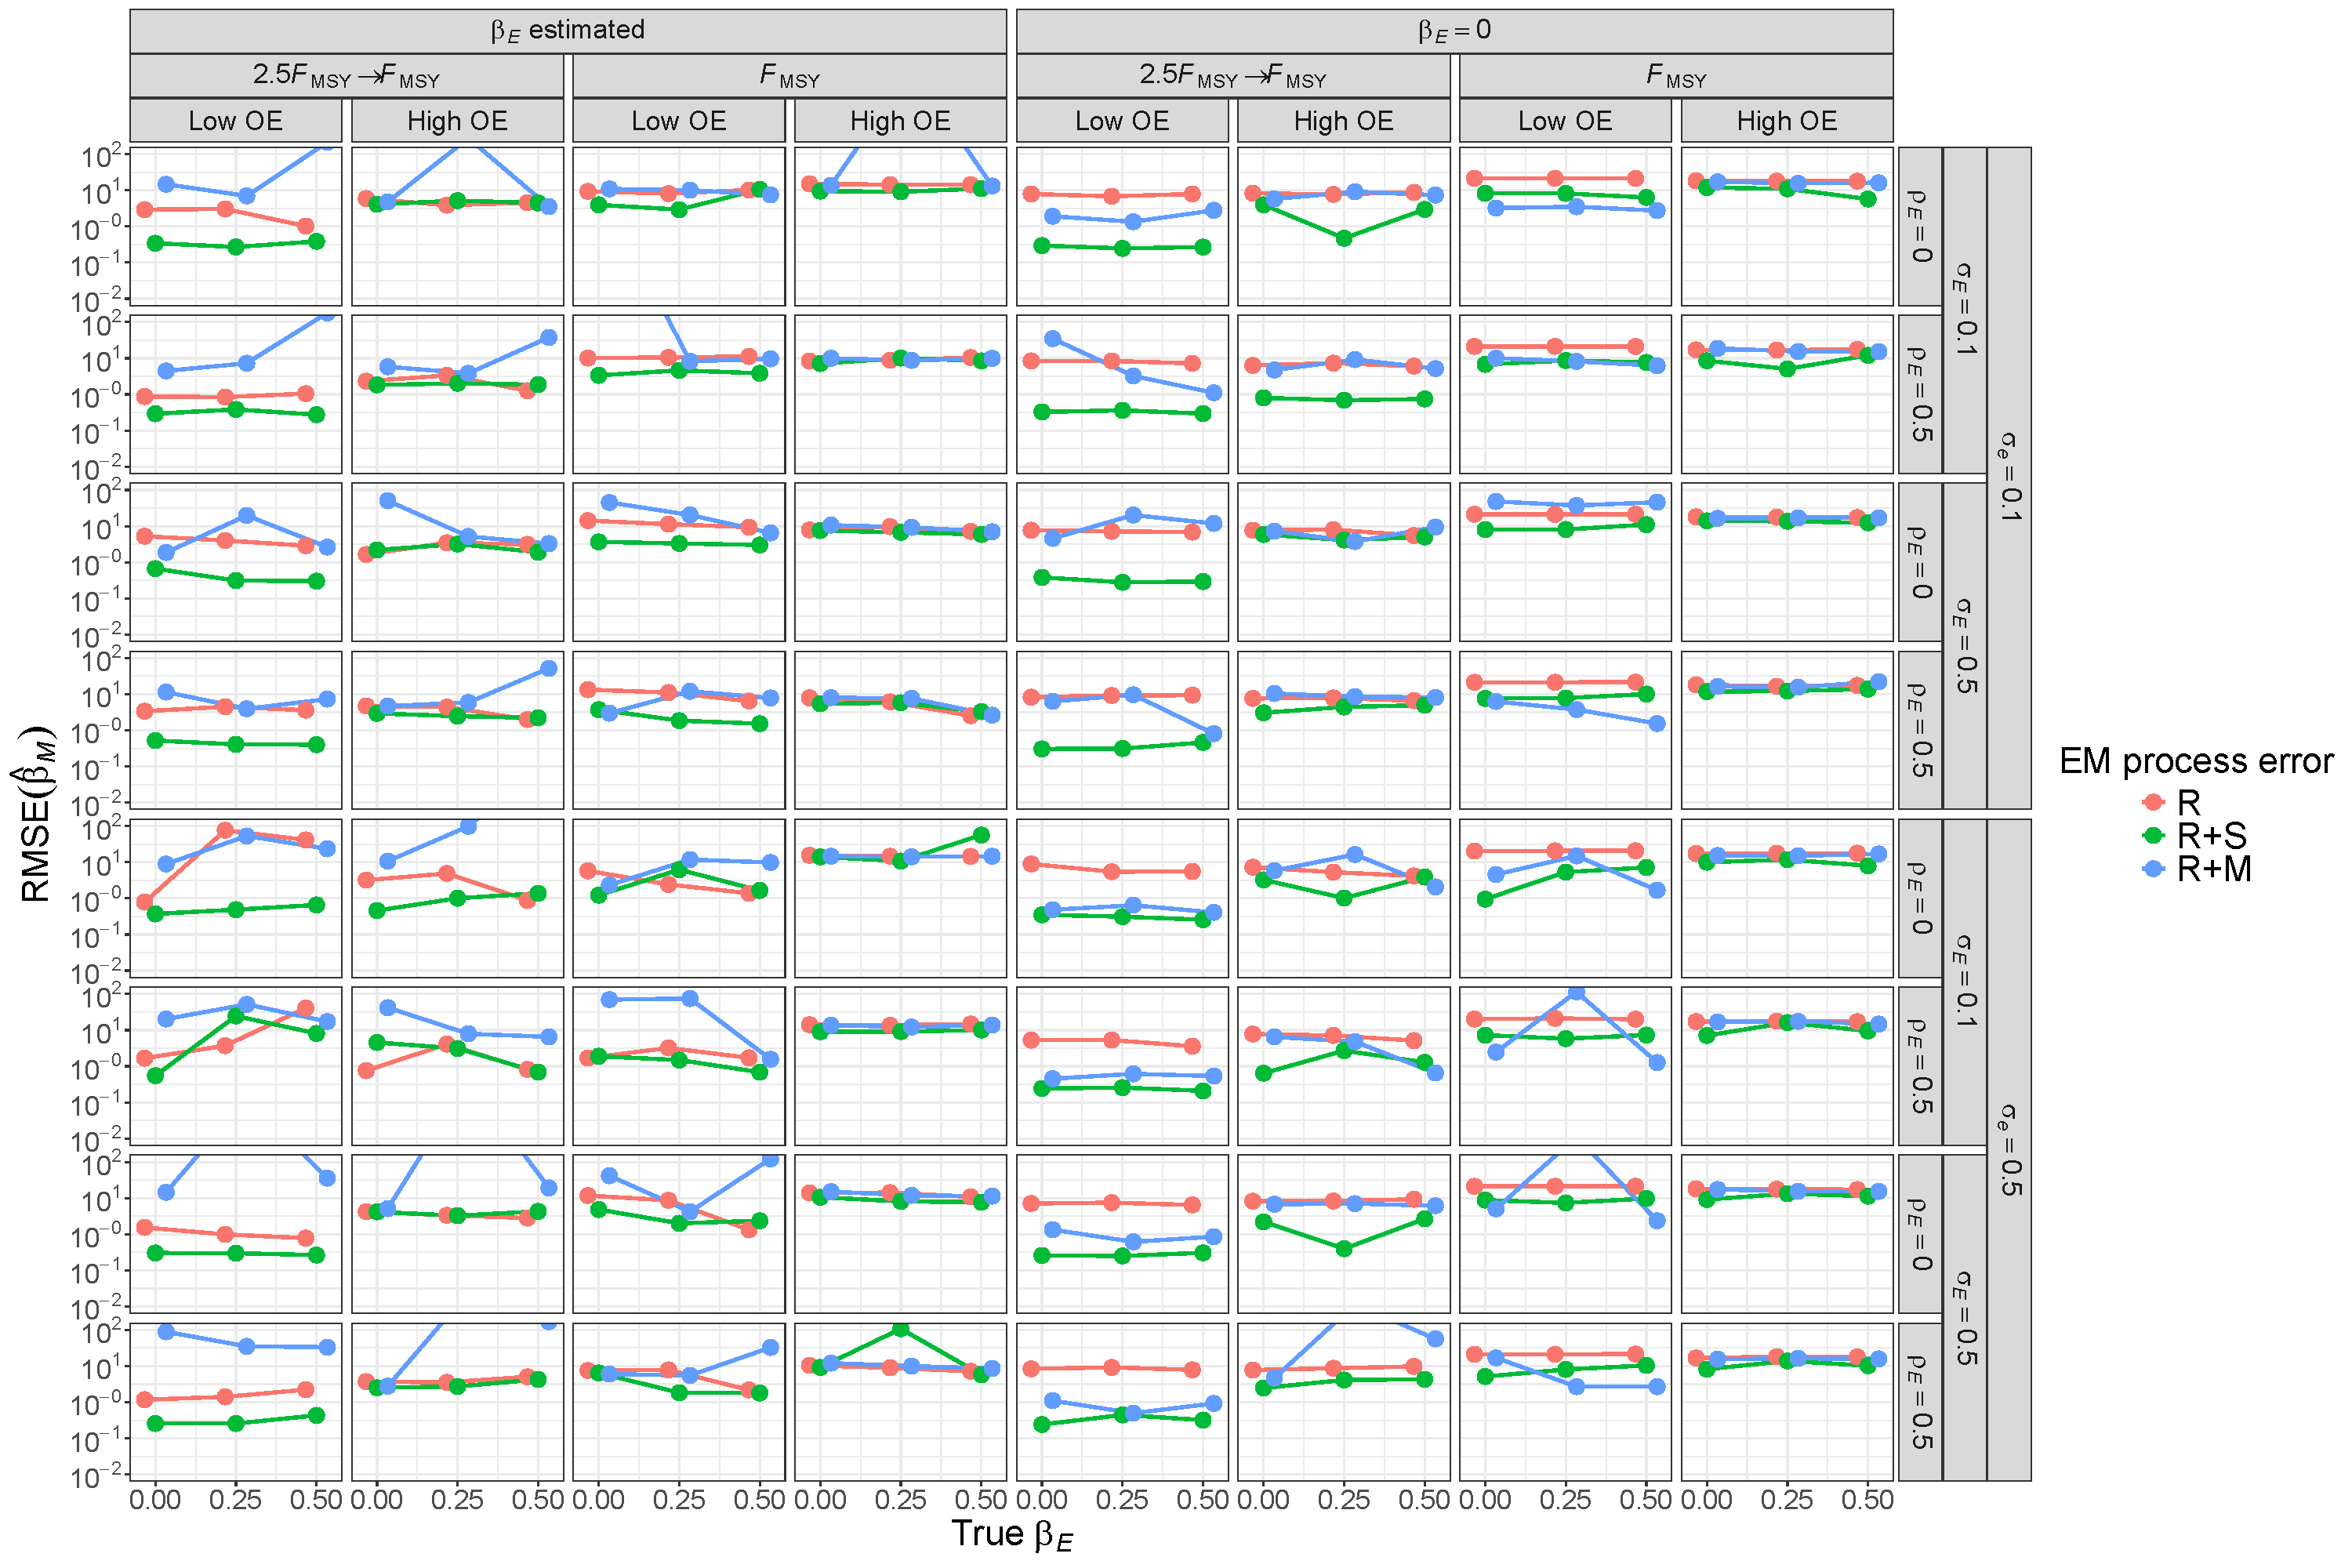
\includegraphics[height = \textheight]{beta_M_rmse_RSom}
%DIFDELCMD < %%%
\DIFdelendFL \DIFaddbeginFL 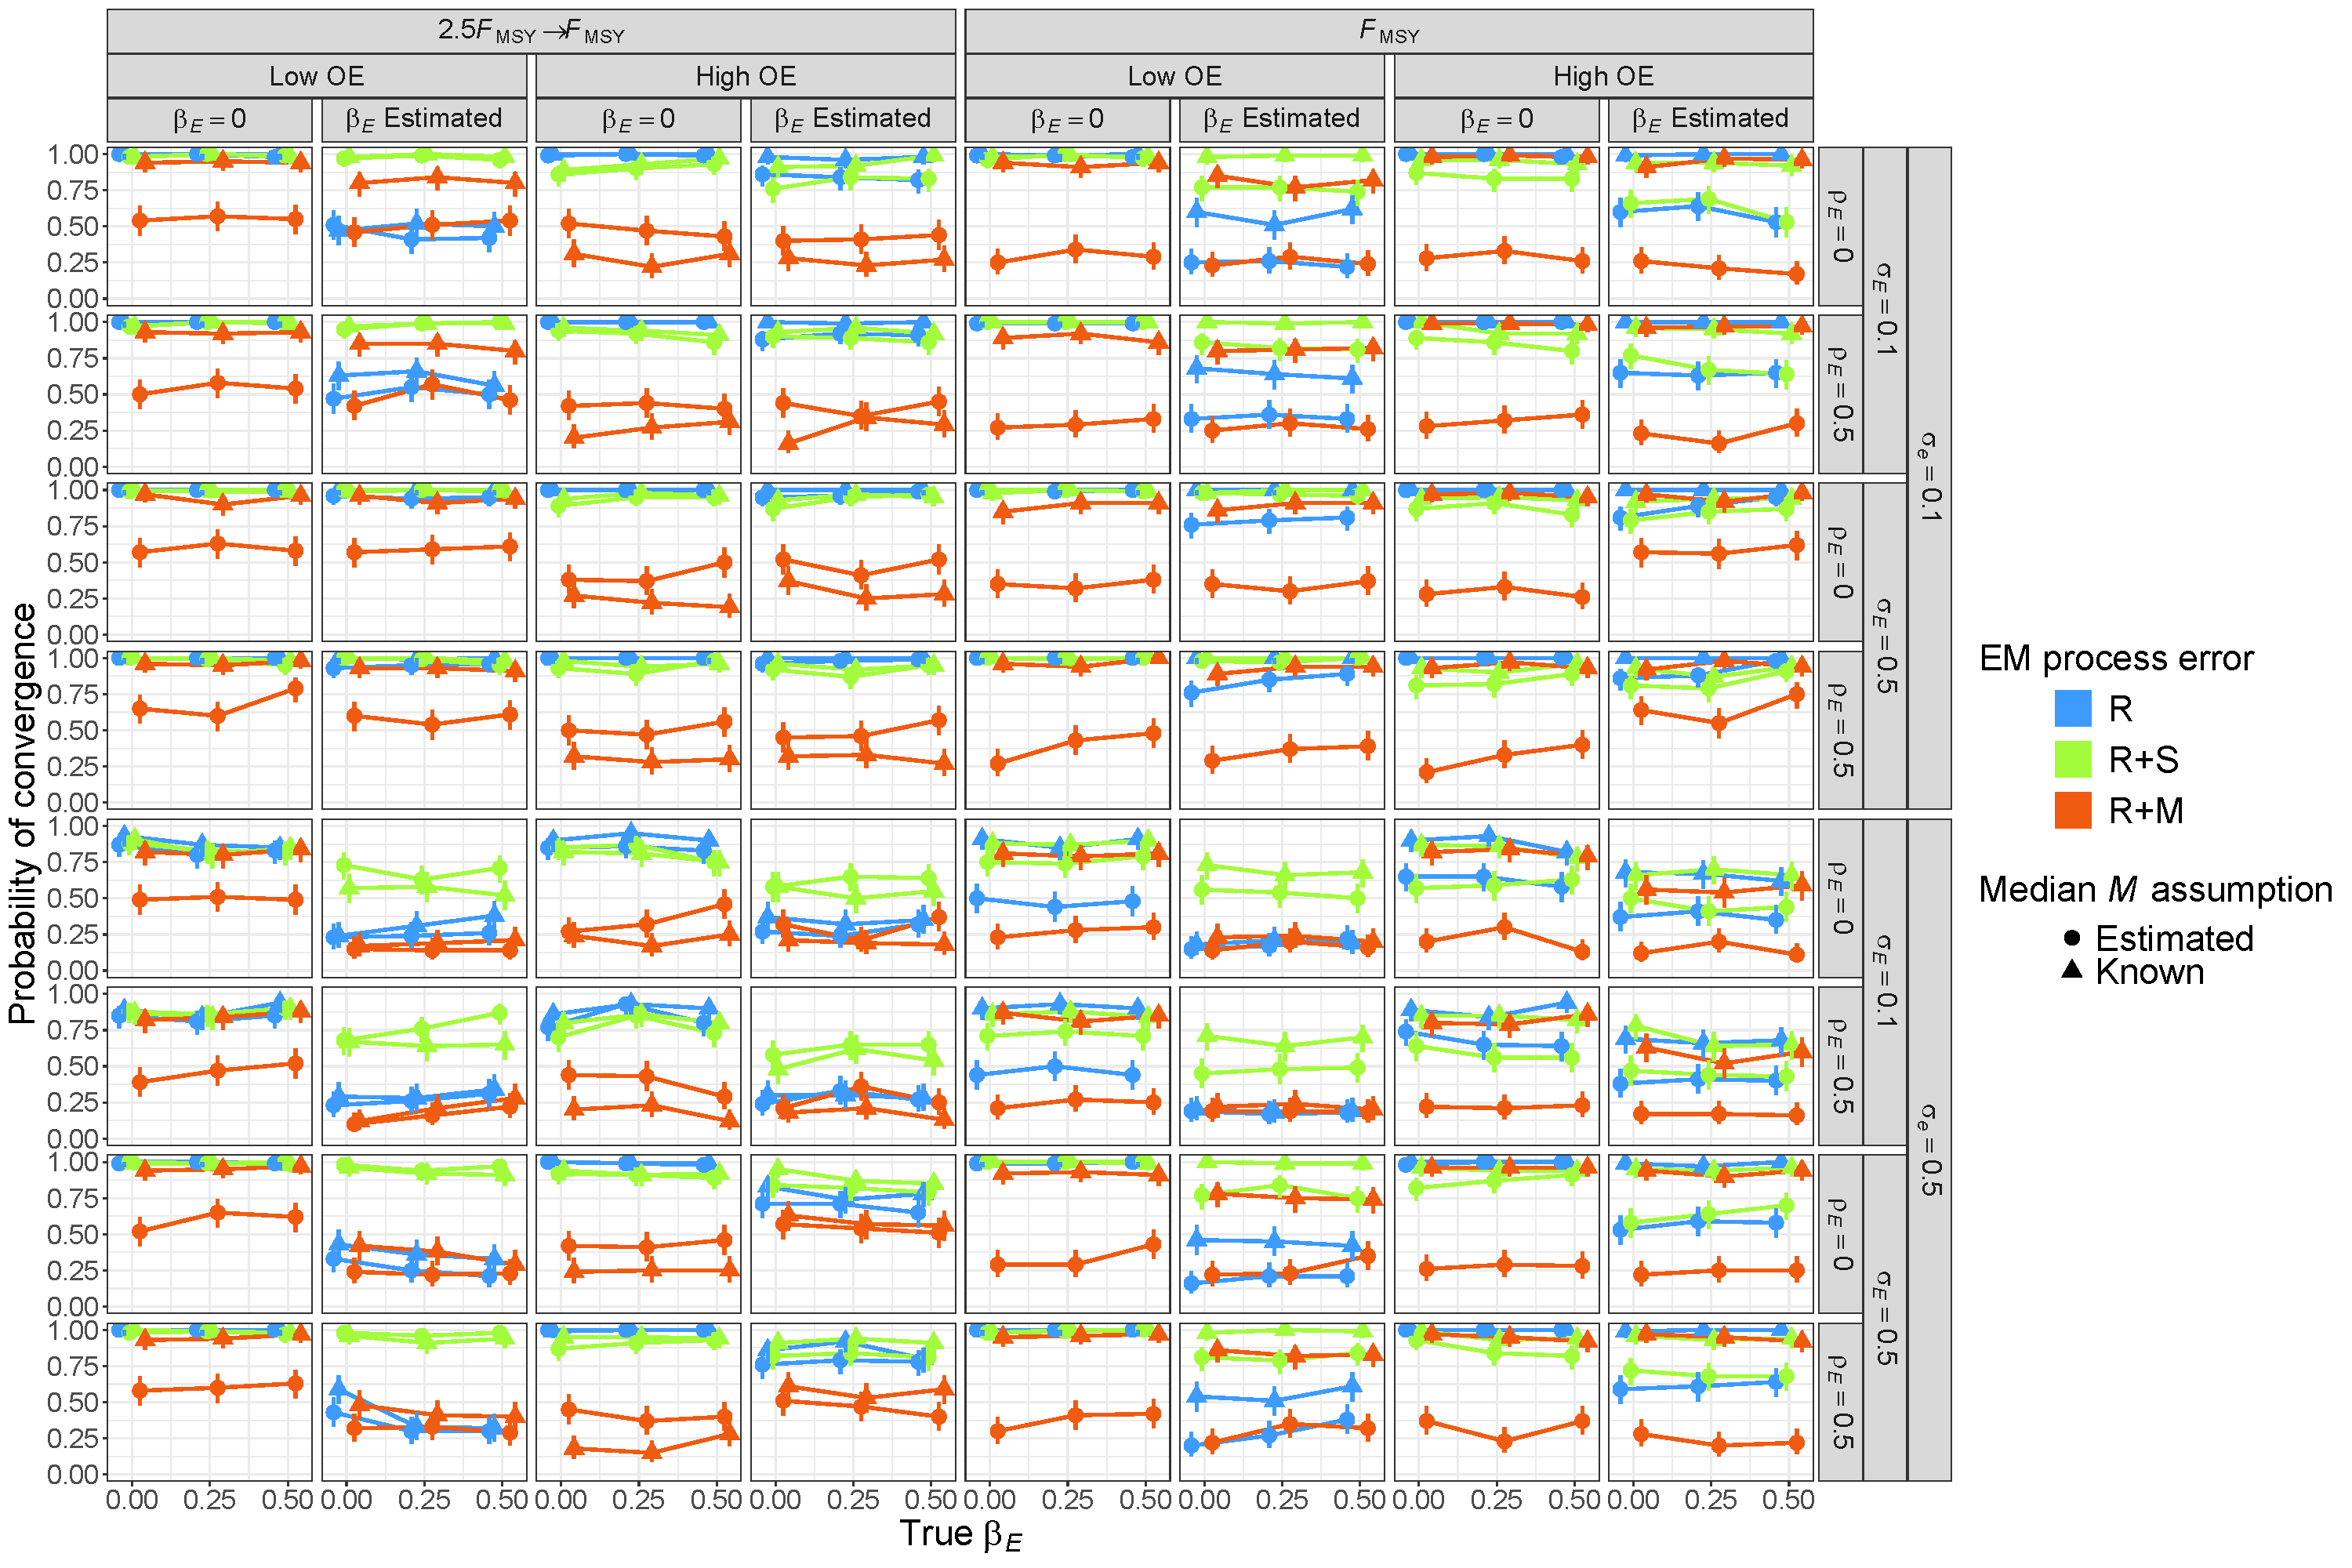
\includegraphics[height = \textheight]{convergence_RSom}
\DIFaddendFL \end{center}
\caption{\DIFdelbeginFL \DIFdelFL{For R+S OMs, RMSE }\DIFdelendFL \DIFaddbeginFL \DIFaddFL{Estimated probability }\DIFaddendFL of \DIFdelbeginFL \DIFdelFL{estimates of  $\beta_M$ from fitting EMs with }\DIFdelendFL \DIFaddbeginFL \DIFaddFL{fits providing Hessian-based standard errors for estimating models assuming }\DIFaddendFL alternative process error\DIFdelbeginFL \DIFdelFL{assumptions }\DIFdelendFL \DIFaddbeginFL \DIFaddFL{, that estimate or assume known median $M$, }\DIFaddendFL and \DIFdelbeginFL \DIFdelFL{treatment }\DIFdelendFL \DIFaddbeginFL \DIFaddFL{that estimate or assume no covariate effect on median $M$ when fitted to R+S operating models and three levels }\DIFaddendFL of \DIFaddbeginFL \DIFaddFL{true }\DIFaddendFL covariate effect \DIFaddbeginFL \DIFaddFL{on median $M$ }\DIFaddendFL (\DIFdelbeginFL \DIFdelFL{$\beta_E = 0$ or estimated}\DIFdelendFL \DIFaddbeginFL \DIFaddFL{x axis}\DIFaddendFL ). \DIFaddbeginFL \DIFaddFL{Vertical lines represent 95\% confidence intervals.}\DIFaddendFL }\DIFdelbeginFL %DIFDELCMD < \label{beta_M_rmse_RSom}
%DIFDELCMD < %%%
\DIFdelendFL \DIFaddbeginFL \label{convergence_RSom}
\DIFaddendFL \end{figure}
\end{landscape}

\begin{landscape}
\begin{figure}
\begin{center}
\DIFdelbeginFL %DIFDELCMD < 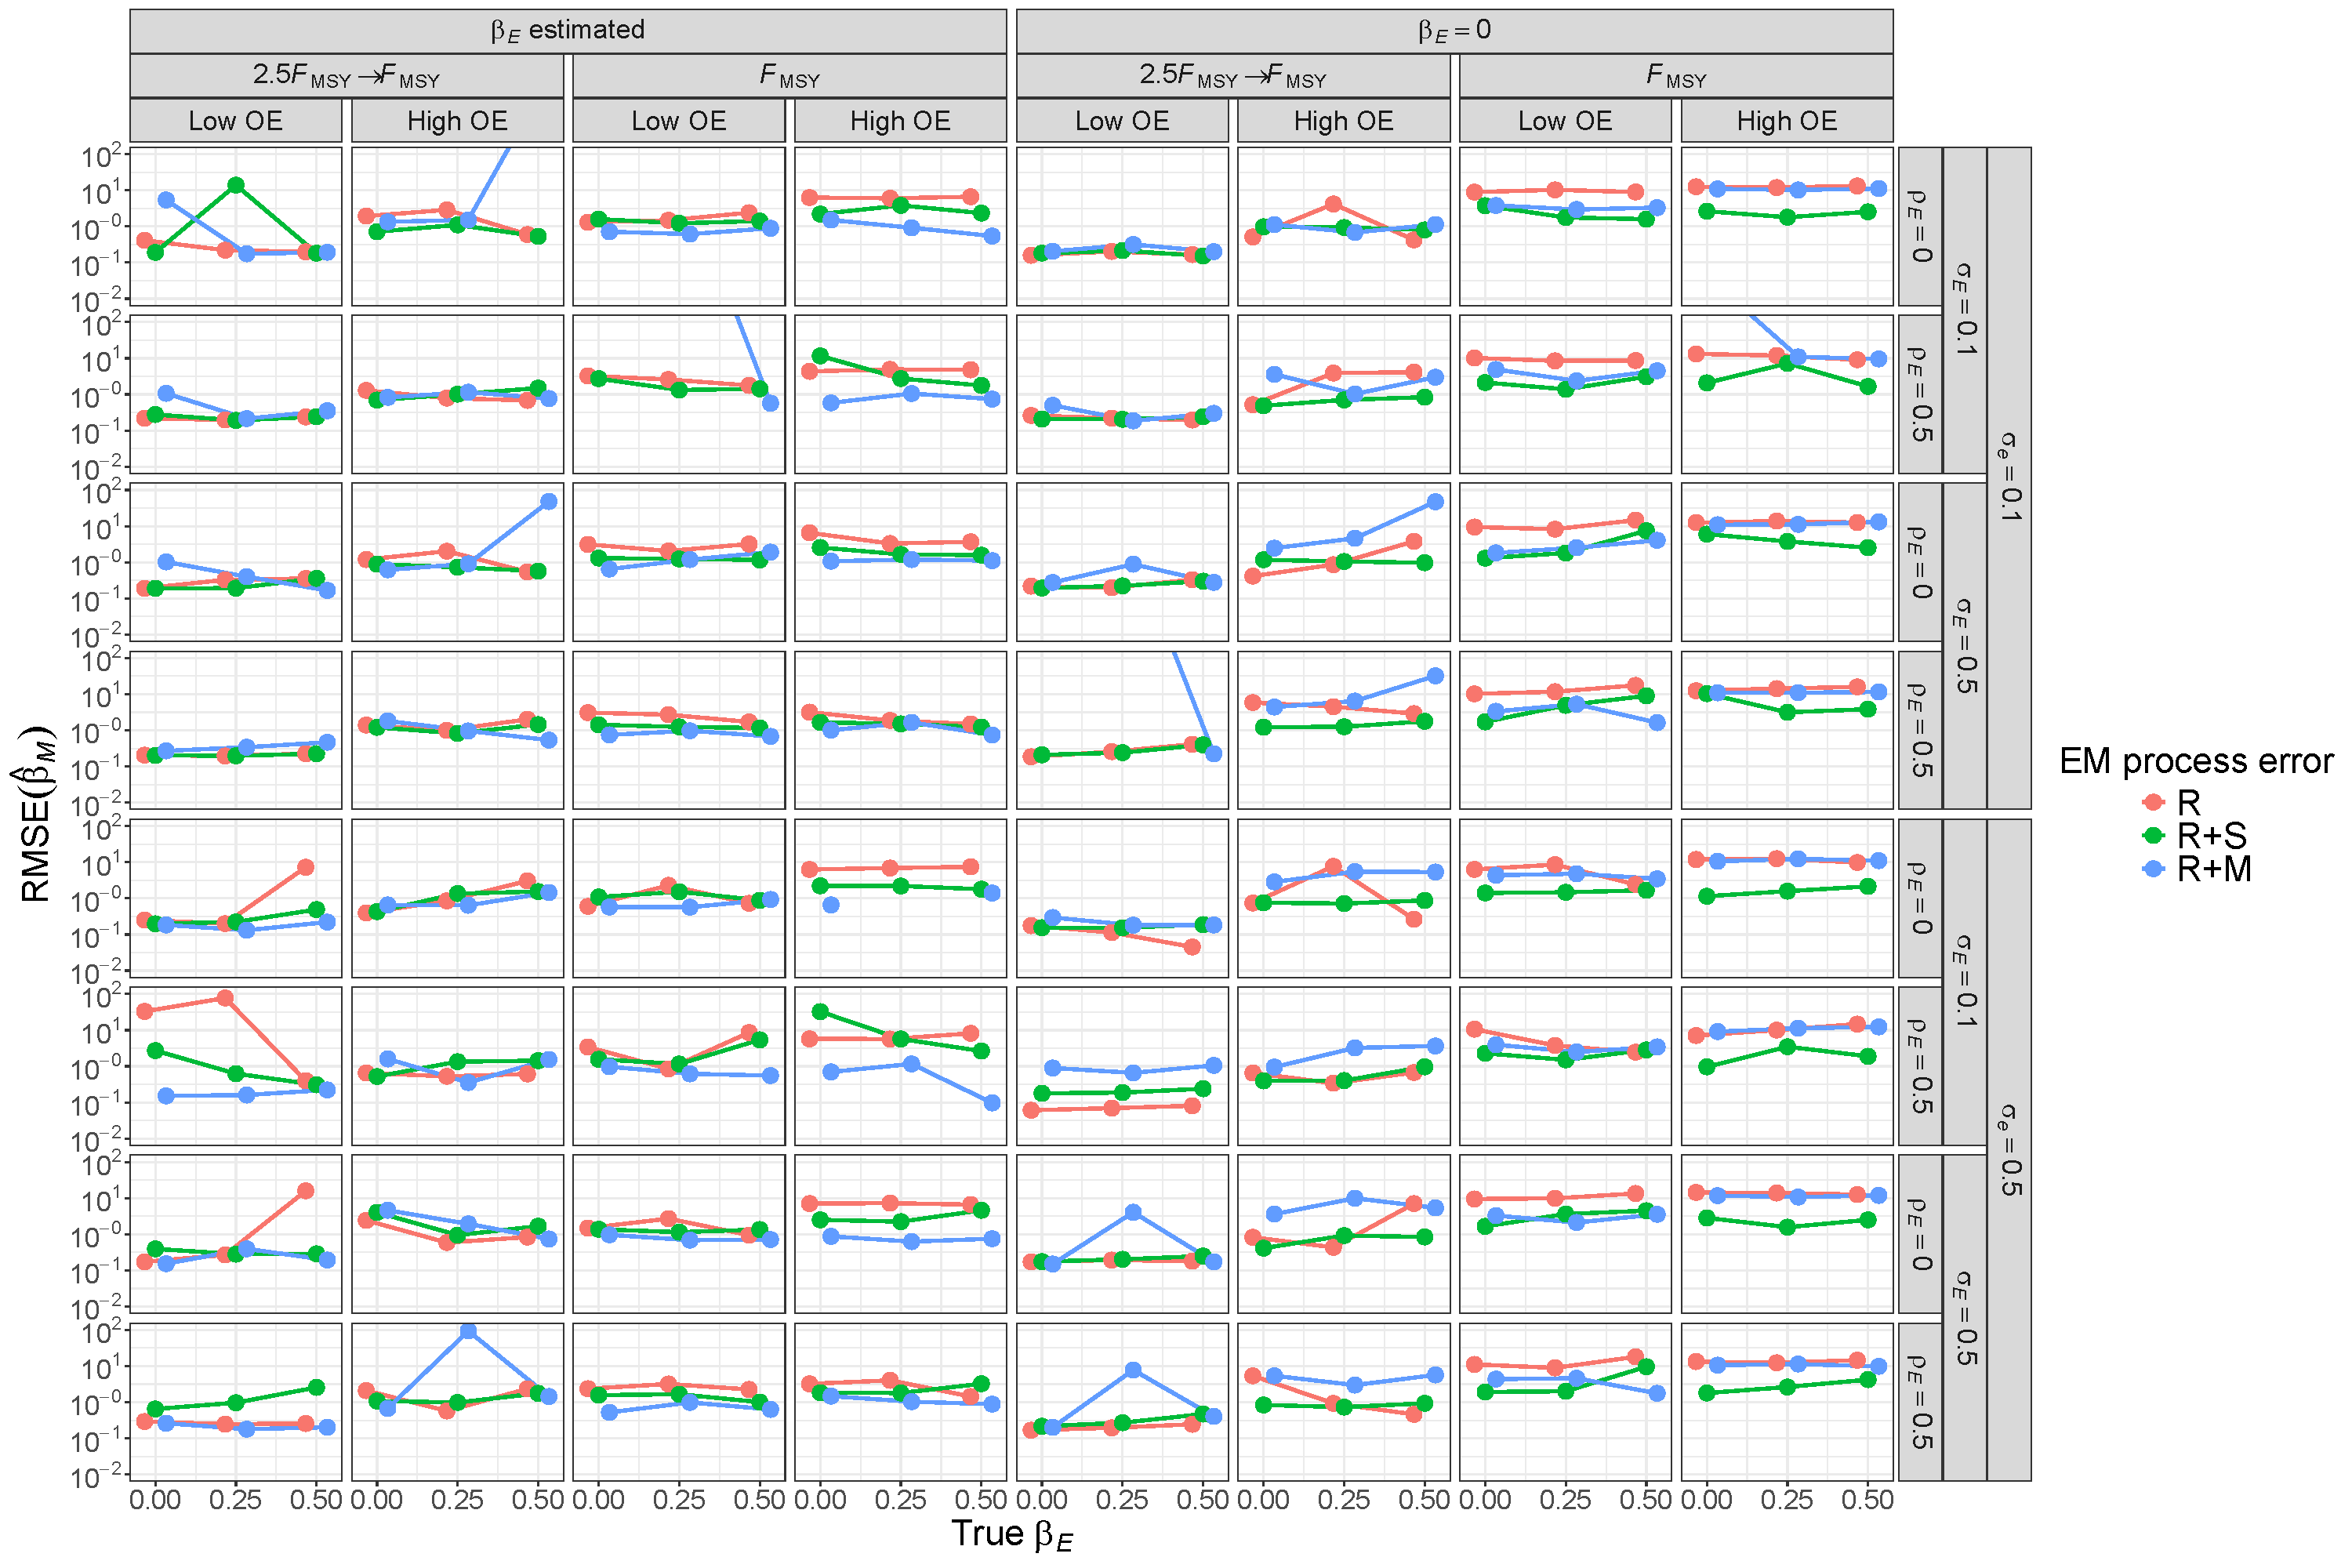
\includegraphics[height = \textheight]{beta_M_rmse_RMom}
%DIFDELCMD < %%%
\DIFdelendFL \DIFaddbeginFL 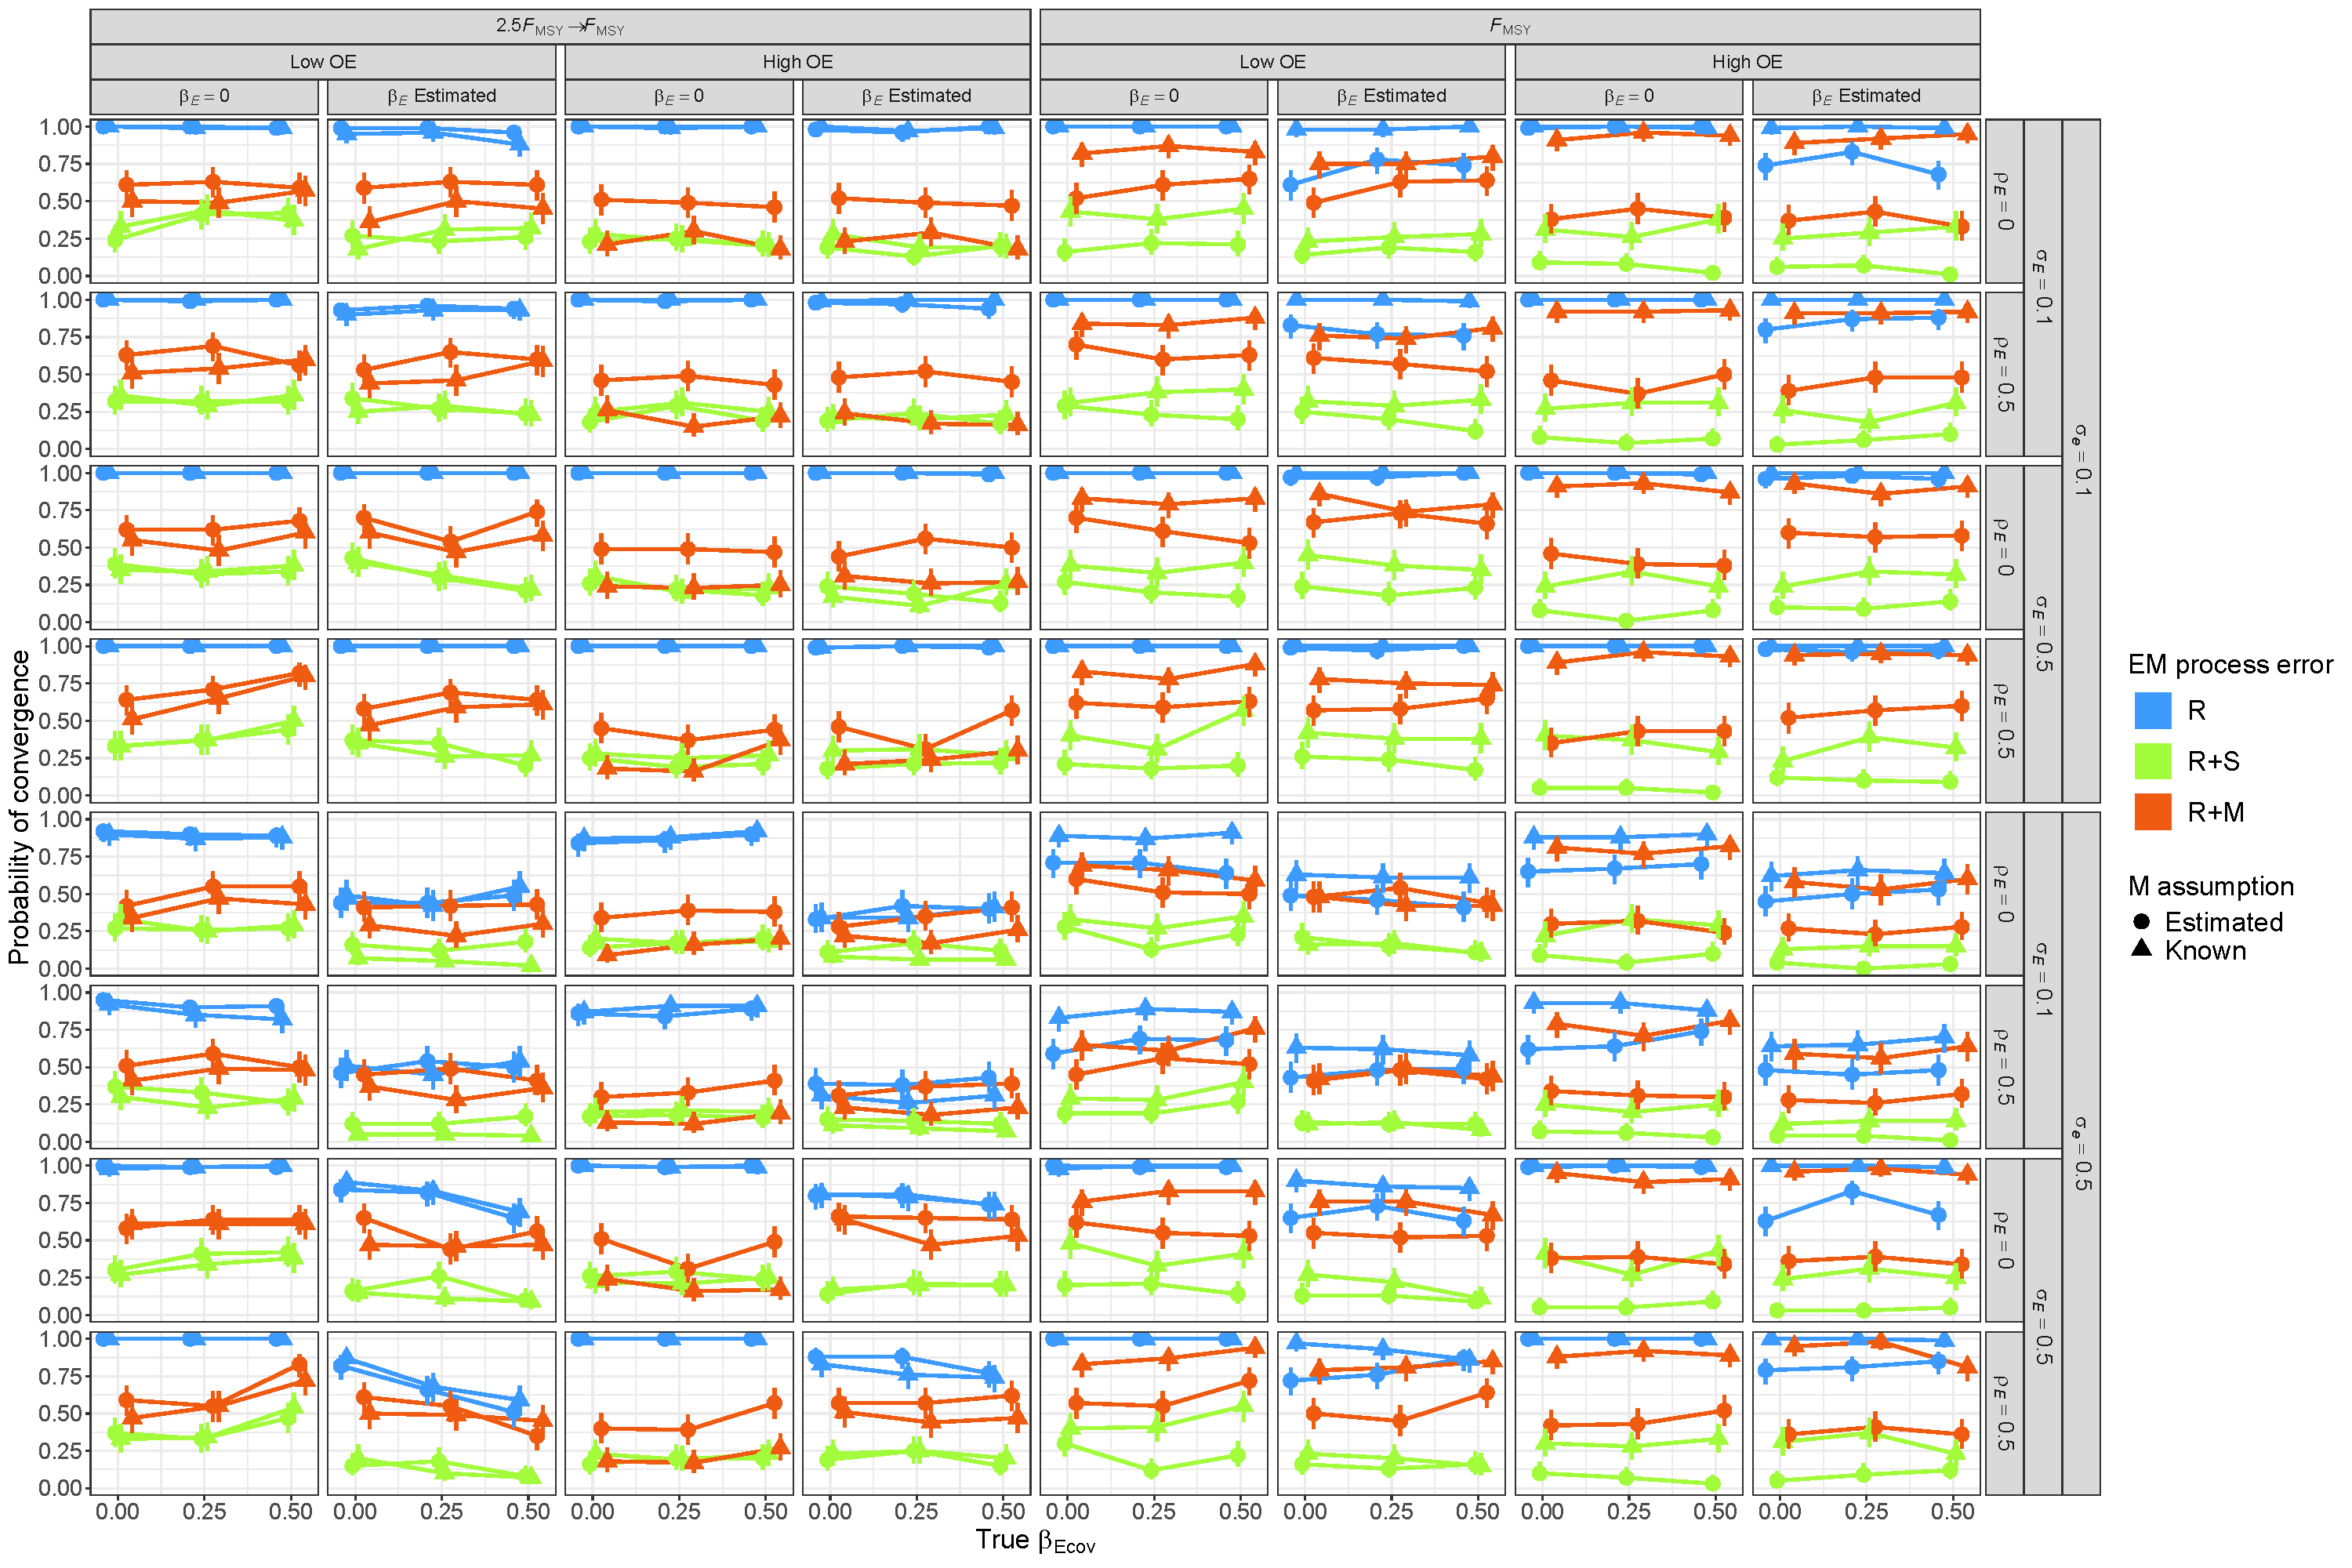
\includegraphics[height = \textheight]{convergence_RMom}
\DIFaddendFL \end{center}
\caption{\DIFdelbeginFL \DIFdelFL{For R+M OMs, RMSE }\DIFdelendFL \DIFaddbeginFL \DIFaddFL{Estimated probability }\DIFaddendFL of \DIFdelbeginFL \DIFdelFL{estimates of  $\beta_M$ from fitting EMs with }\DIFdelendFL \DIFaddbeginFL \DIFaddFL{fits providing Hessian-based standard errors for estimating models assuming }\DIFaddendFL alternative process error\DIFdelbeginFL \DIFdelFL{assumptions }\DIFdelendFL \DIFaddbeginFL \DIFaddFL{, that estimate or assume known median $M$, }\DIFaddendFL and \DIFdelbeginFL \DIFdelFL{treatment }\DIFdelendFL \DIFaddbeginFL \DIFaddFL{that estimate or assume no covariate effect on median $M$ when fitted to R+M operating models and three levels }\DIFaddendFL of \DIFaddbeginFL \DIFaddFL{true }\DIFaddendFL covariate effect \DIFaddbeginFL \DIFaddFL{on median $M$ }\DIFaddendFL (\DIFdelbeginFL \DIFdelFL{$\beta_E = 0$ or estimated}\DIFdelendFL \DIFaddbeginFL \DIFaddFL{x axis}\DIFaddendFL ). \DIFaddbeginFL \DIFaddFL{Vertical lines represent 95\% confidence intervals.}\DIFaddendFL }\DIFdelbeginFL %DIFDELCMD < \label{beta_M_rmse_RMom}
%DIFDELCMD < %%%
\DIFdelendFL \DIFaddbeginFL \label{convergence_RMom}
\DIFaddendFL \end{figure}
\end{landscape}

\DIFdelbegin \subsection*{\DIFdel{Terminal year natural mortality bias}}%DIFAUXCMD
%DIFDELCMD < \label{terminal-year-natural-mortality-bias}
%DIFDELCMD < %%%
\addcontentsline{toc}{subsection}{\DIFdel{Terminal year natural mortality bias}}
%DIFAUXCMD
%DIFDELCMD < 

%DIFDELCMD < %%%
\DIFdelend \begin{landscape}
\begin{figure}
\begin{center}
\DIFdelbeginFL %DIFDELCMD < 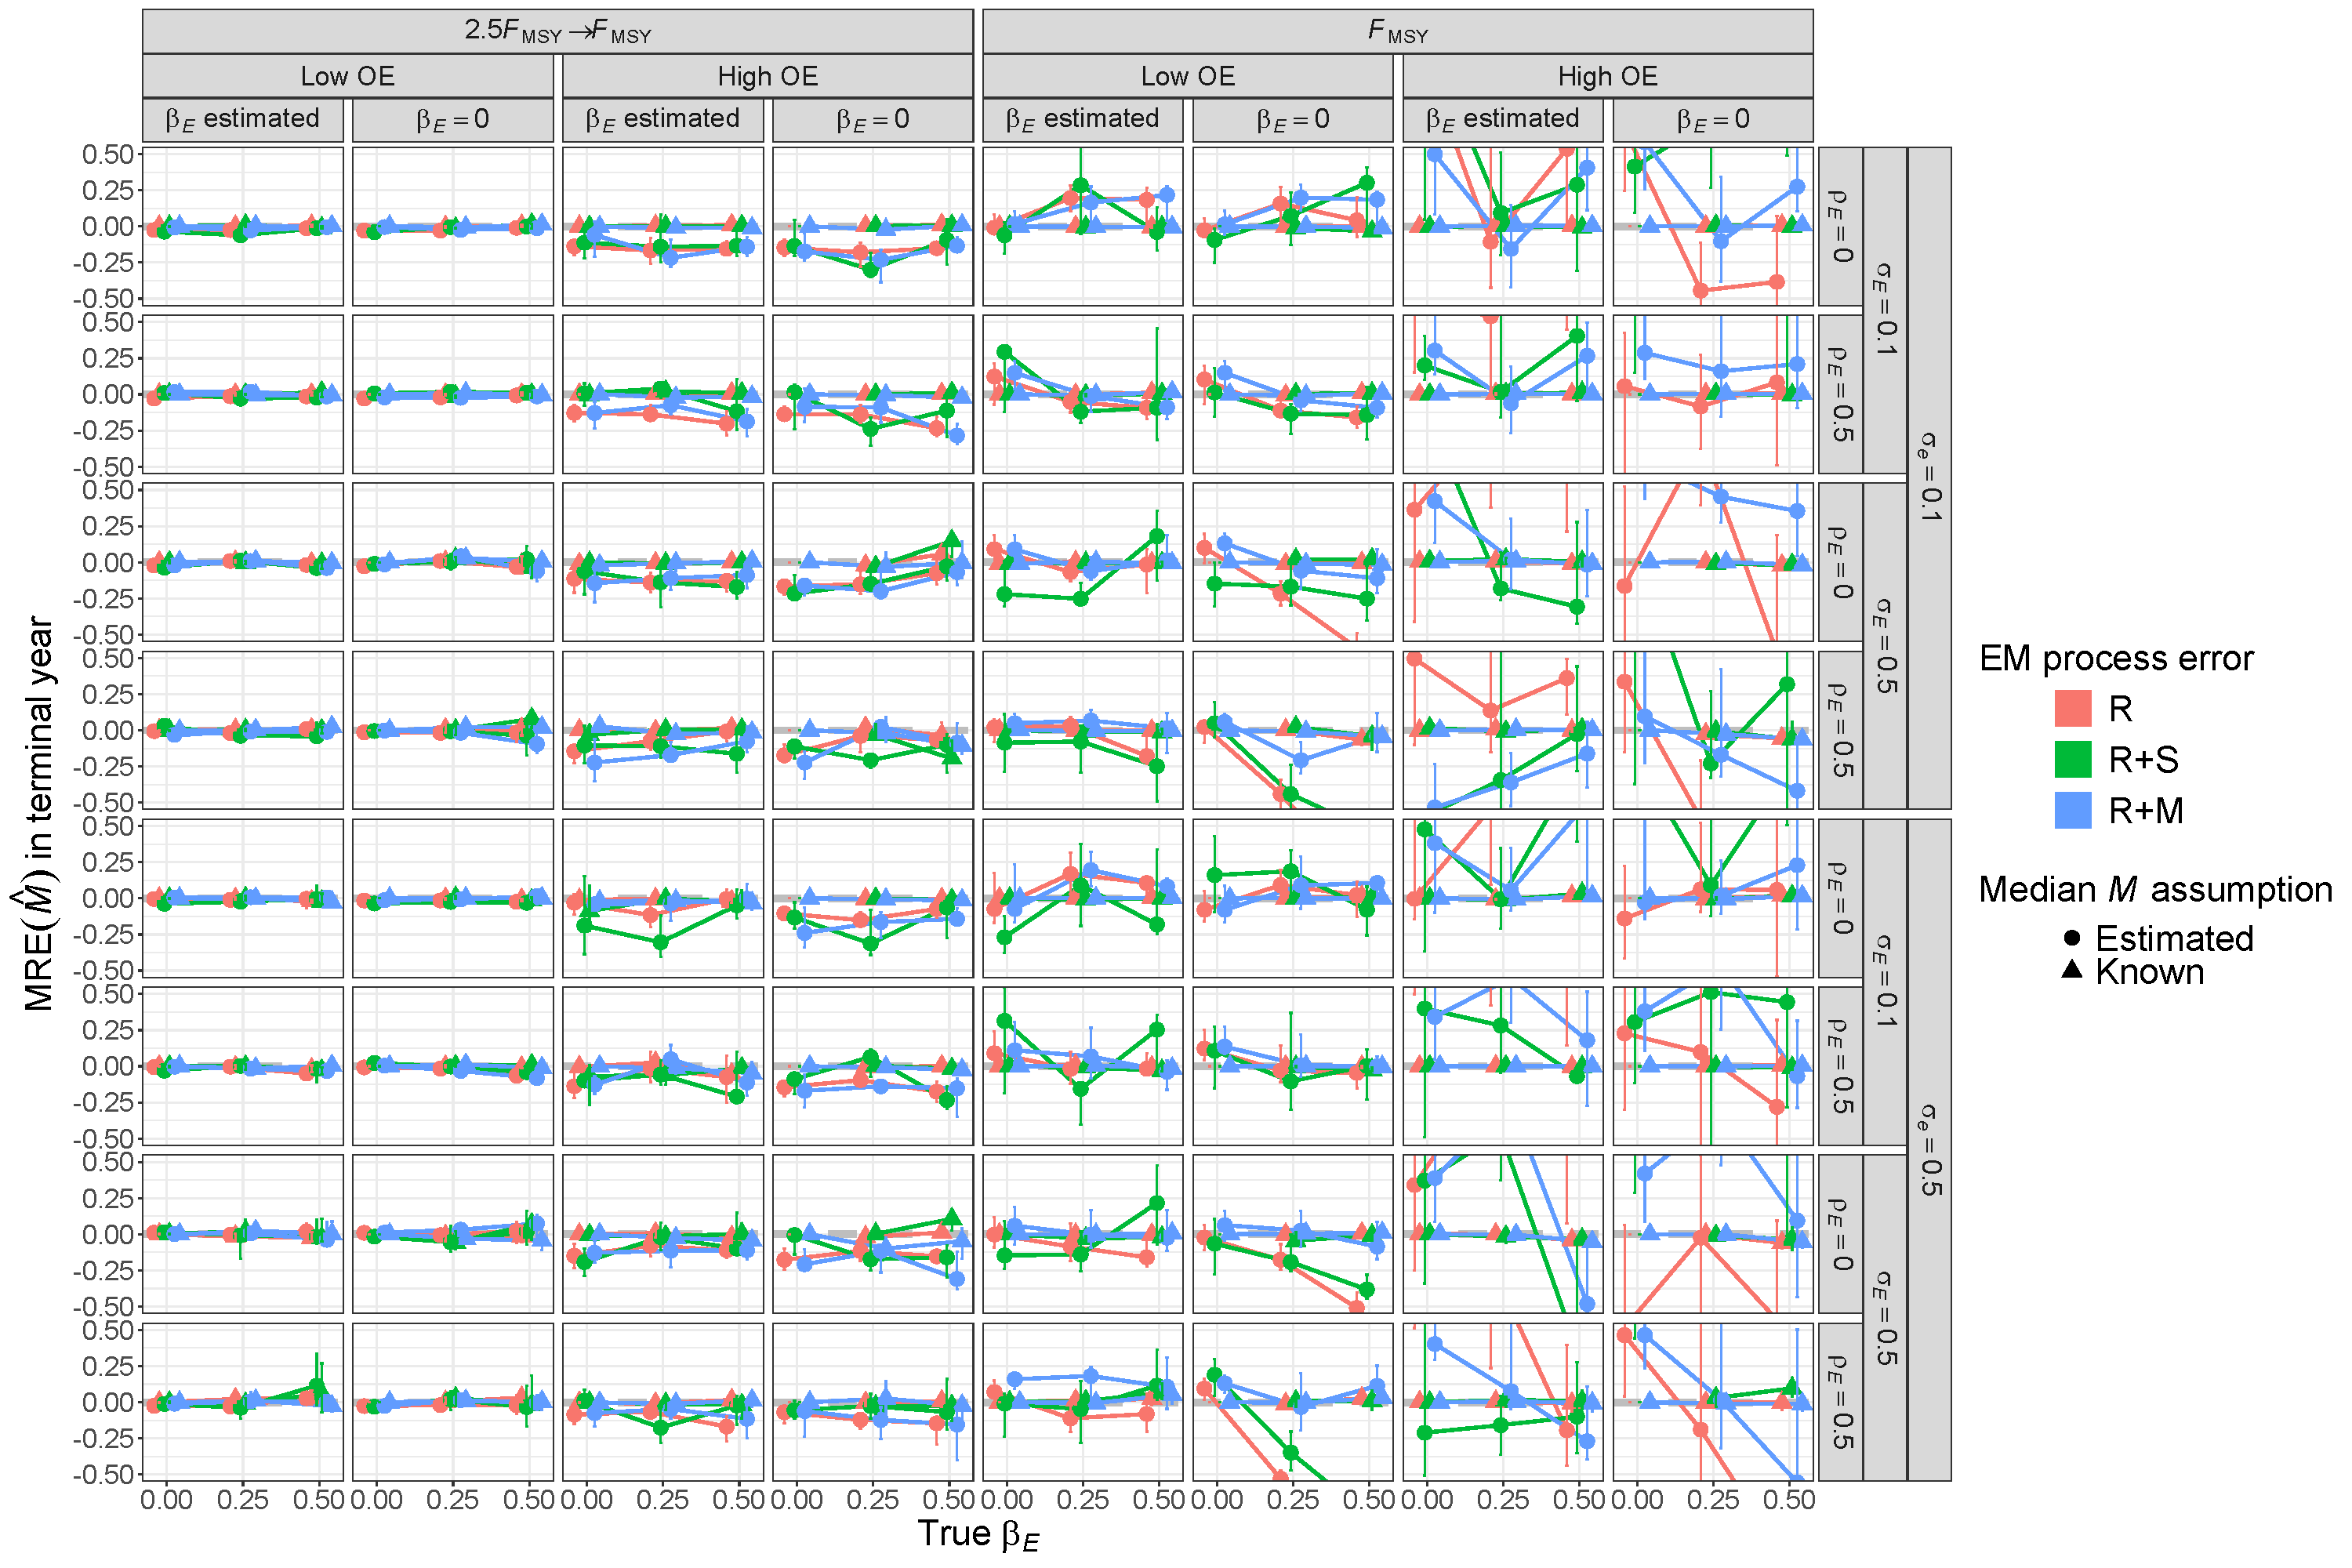
\includegraphics[height = \textheight]{terminal_year_M_bias_Rom}
%DIFDELCMD < %%%
\DIFdelendFL \DIFaddbeginFL 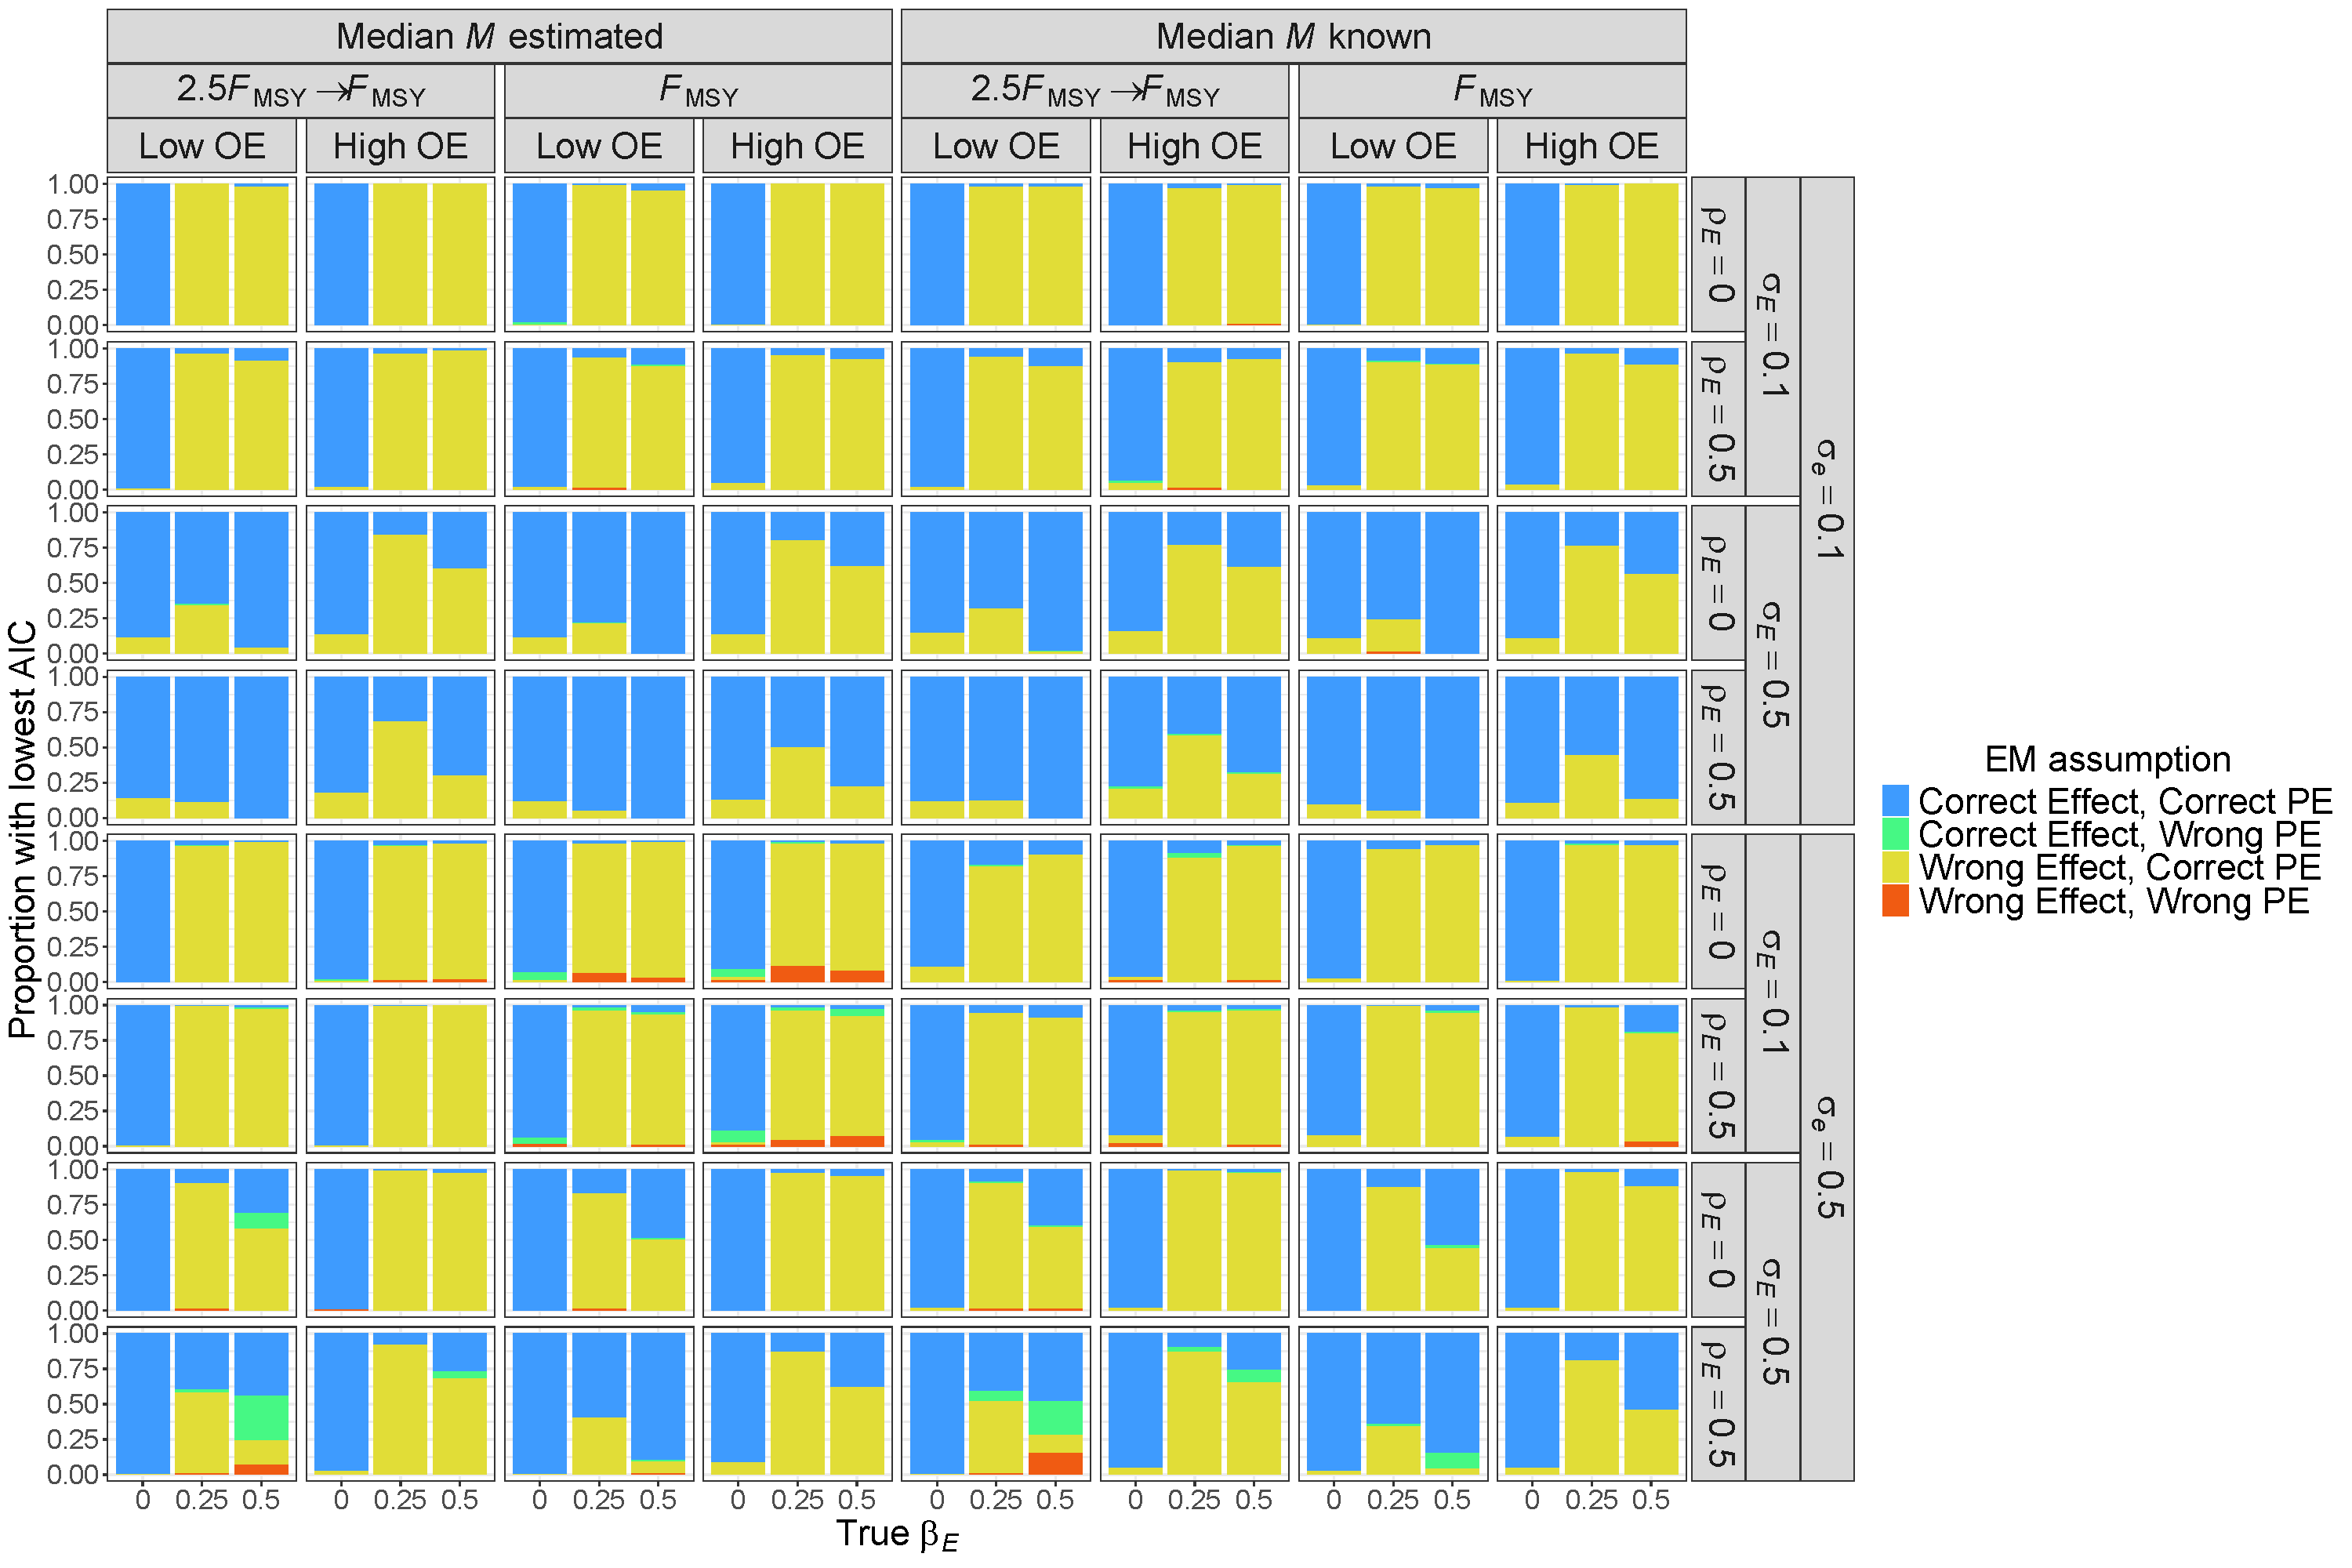
\includegraphics[height = \textheight]{aic_Rom}
\DIFaddendFL \end{center}
\caption{\DIFdelbeginFL \DIFdelFL{For R OMs, median relative error (MRE) }\DIFdelendFL \DIFaddbeginFL \DIFaddFL{Proportion }\DIFaddendFL of \DIFdelbeginFL \DIFdelFL{estimates of terminal year $M$ }\DIFdelendFL \DIFaddbeginFL \DIFaddFL{simulated data sets }\DIFaddendFL for \DIFdelbeginFL \DIFdelFL{EMs with alternative process error assumptions, }\DIFdelendFL \DIFaddbeginFL \DIFaddFL{R operating models where the estimating model type (}\DIFaddendFL treatment of \DIFaddbeginFL \DIFaddFL{environmental }\DIFaddendFL covariate \DIFdelbeginFL \DIFdelFL{effect ($\beta_E = 0$ or estimated), }\DIFdelendFL and \DIFdelbeginFL \DIFdelFL{treatment of median $M$ parameter ($\beta_M$ estimated or known}\DIFdelendFL \DIFaddbeginFL \DIFaddFL{assumed process error type}\DIFaddendFL ) \DIFaddbeginFL \DIFaddFL{had the lowest AIC}\DIFaddendFL .}\DIFdelbeginFL %DIFDELCMD < \label{terminal_M_bias_Rom}
%DIFDELCMD < %%%
\DIFdelendFL \DIFaddbeginFL \label{aic_Rom}
\DIFaddendFL \end{figure}
\end{landscape}

\begin{landscape}
\begin{figure}
\begin{center}
\DIFdelbeginFL %DIFDELCMD < 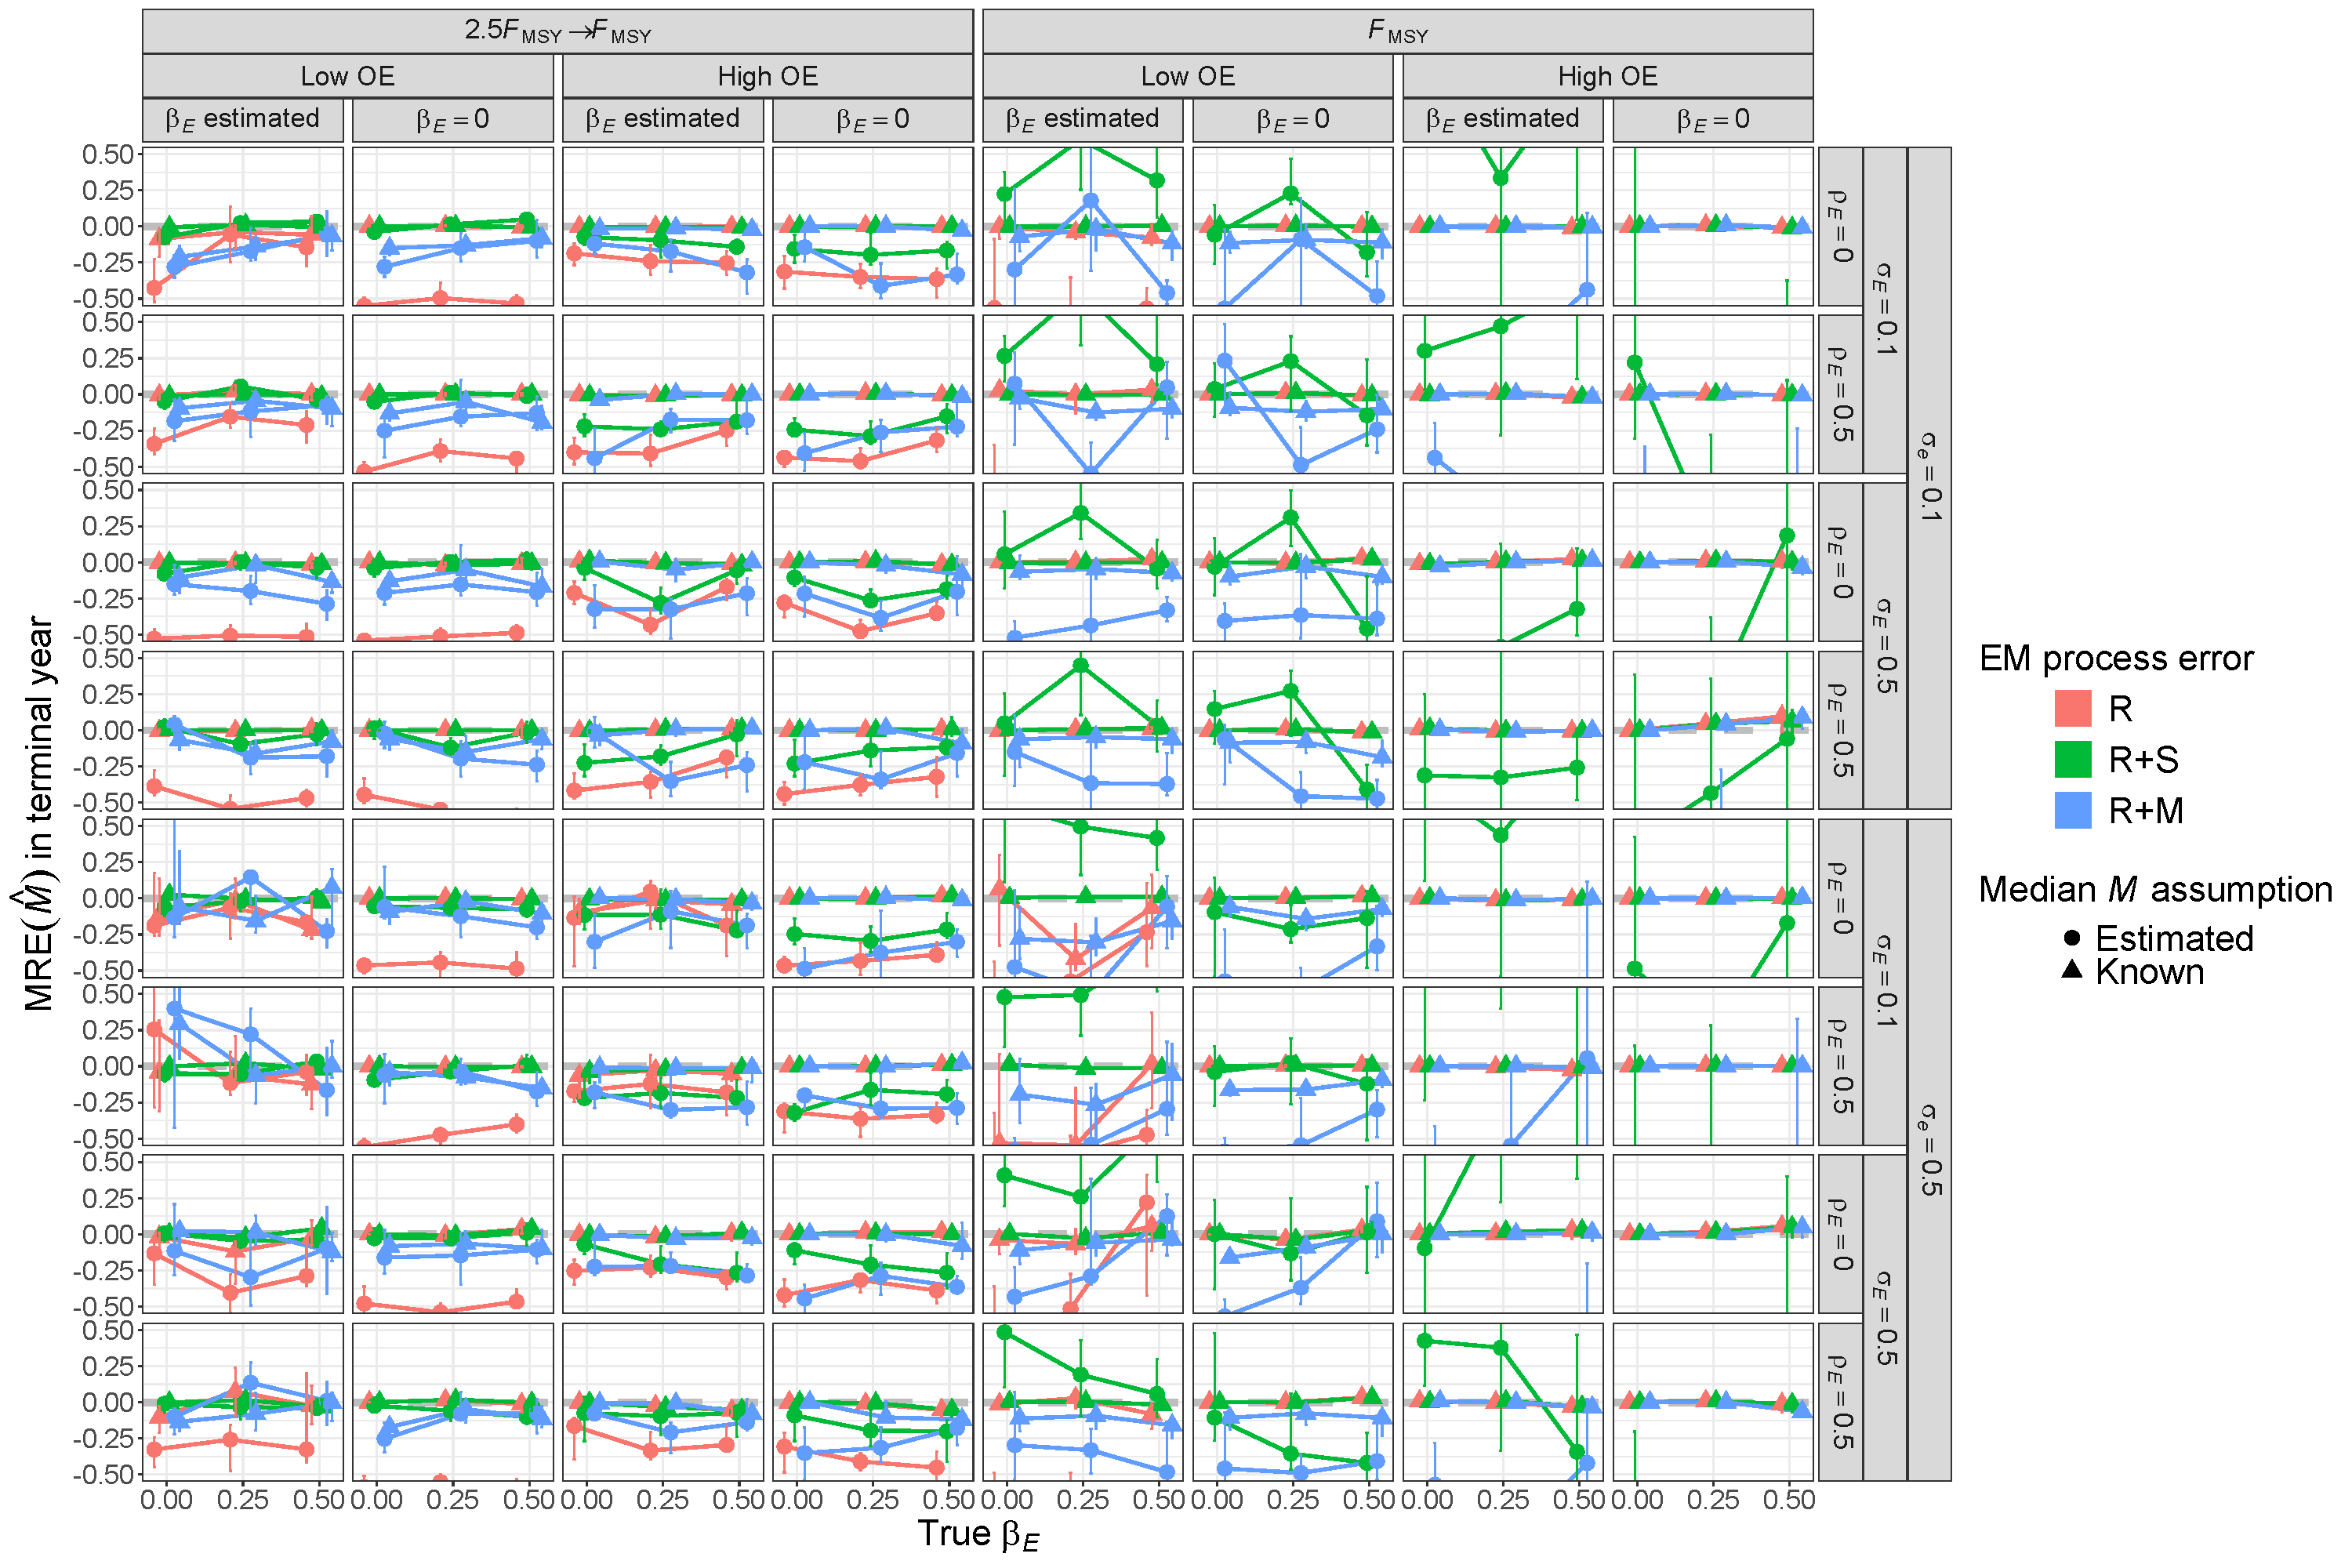
\includegraphics[height = \textheight]{terminal_year_M_bias_RSom}
%DIFDELCMD < %%%
\DIFdelendFL \DIFaddbeginFL 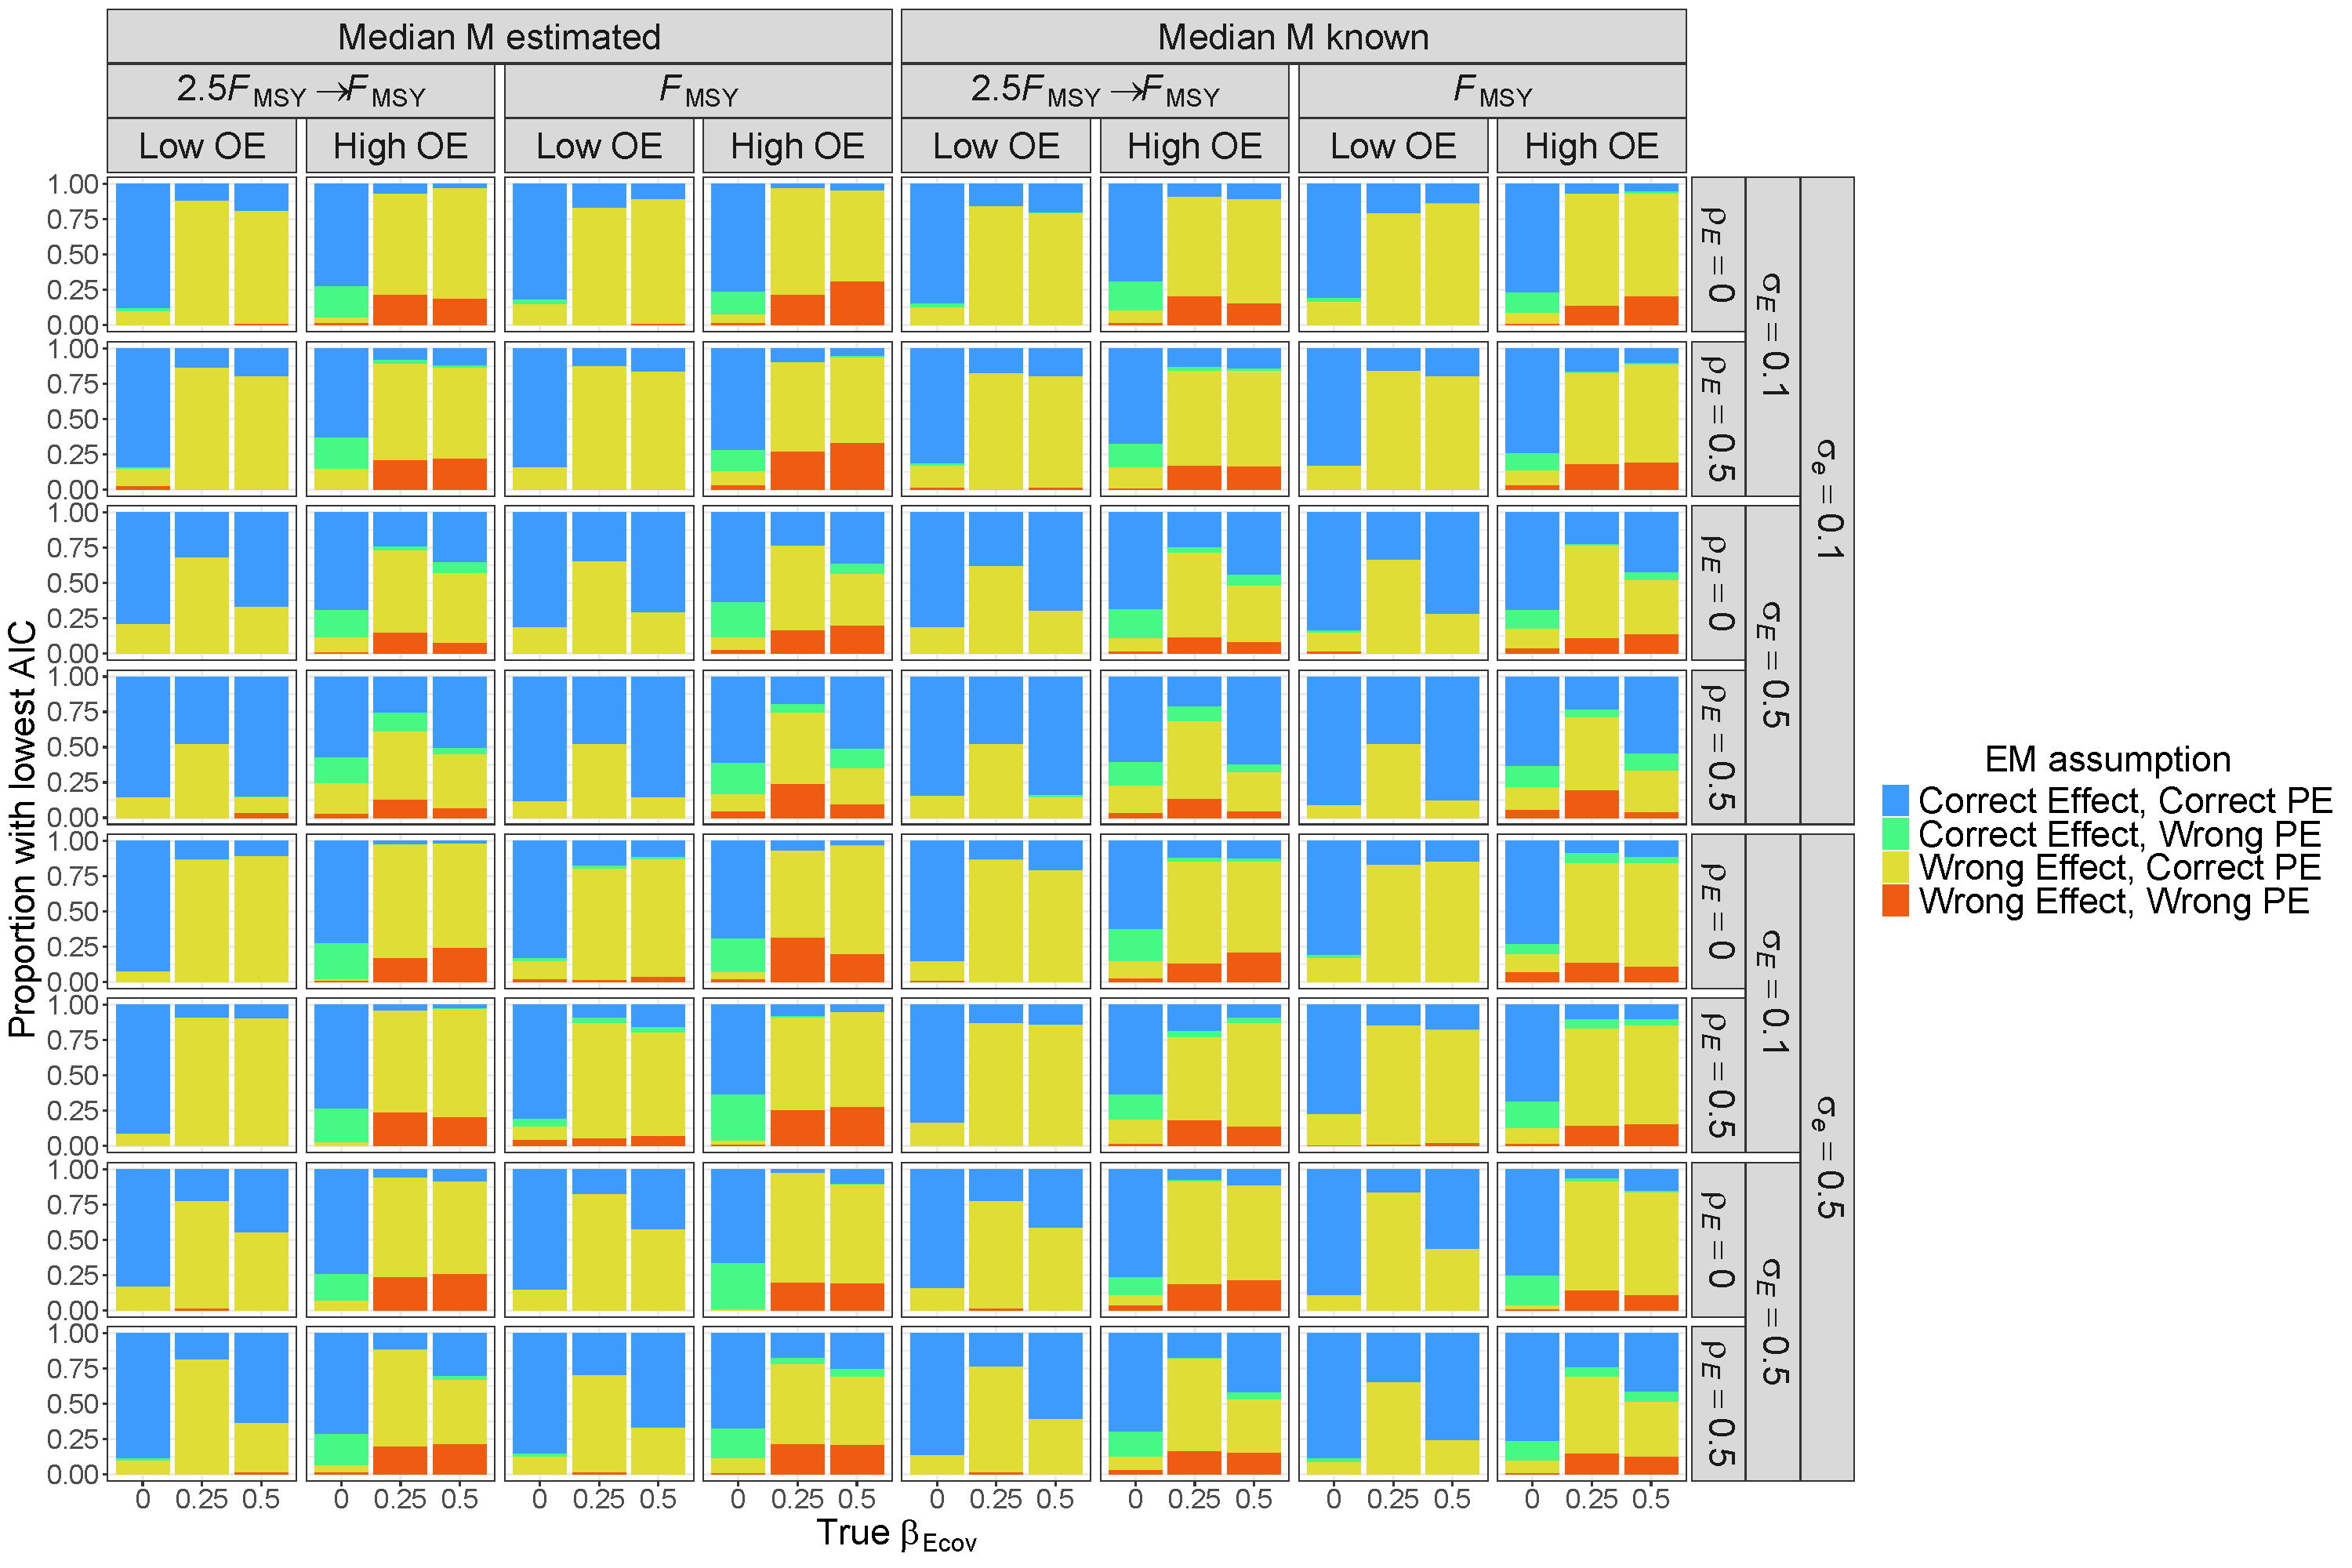
\includegraphics[height = \textheight]{aic_RSom}
\DIFaddendFL \end{center}
\caption{\DIFdelbeginFL \DIFdelFL{For }\DIFdelendFL \DIFaddbeginFL \DIFaddFL{Proportion of simulated data sets for }\DIFaddendFL R+S \DIFdelbeginFL \DIFdelFL{OMs, median relative error }\DIFdelendFL \DIFaddbeginFL \DIFaddFL{operating models where the estimating model type }\DIFaddendFL (\DIFdelbeginFL \DIFdelFL{MRE) of estimates of terminal year $M$ for EMs with alternative process error assumptions, }\DIFdelendFL treatment of \DIFaddbeginFL \DIFaddFL{environmental }\DIFaddendFL covariate \DIFdelbeginFL \DIFdelFL{effect ($\beta_E = 0$ or estimated), }\DIFdelendFL and \DIFdelbeginFL \DIFdelFL{treatment of median $M$ parameter ($\beta_M$ estimated or known}\DIFdelendFL \DIFaddbeginFL \DIFaddFL{assumed process error type}\DIFaddendFL ) \DIFaddbeginFL \DIFaddFL{had the lowest AIC}\DIFaddendFL .}\DIFdelbeginFL %DIFDELCMD < \label{terminal_M_bias_RSom}
%DIFDELCMD < %%%
\DIFdelendFL \DIFaddbeginFL \label{aic_RSom}
\DIFaddendFL \end{figure}
\end{landscape}

\begin{landscape}
\begin{figure}
\begin{center}
\DIFdelbeginFL %DIFDELCMD < 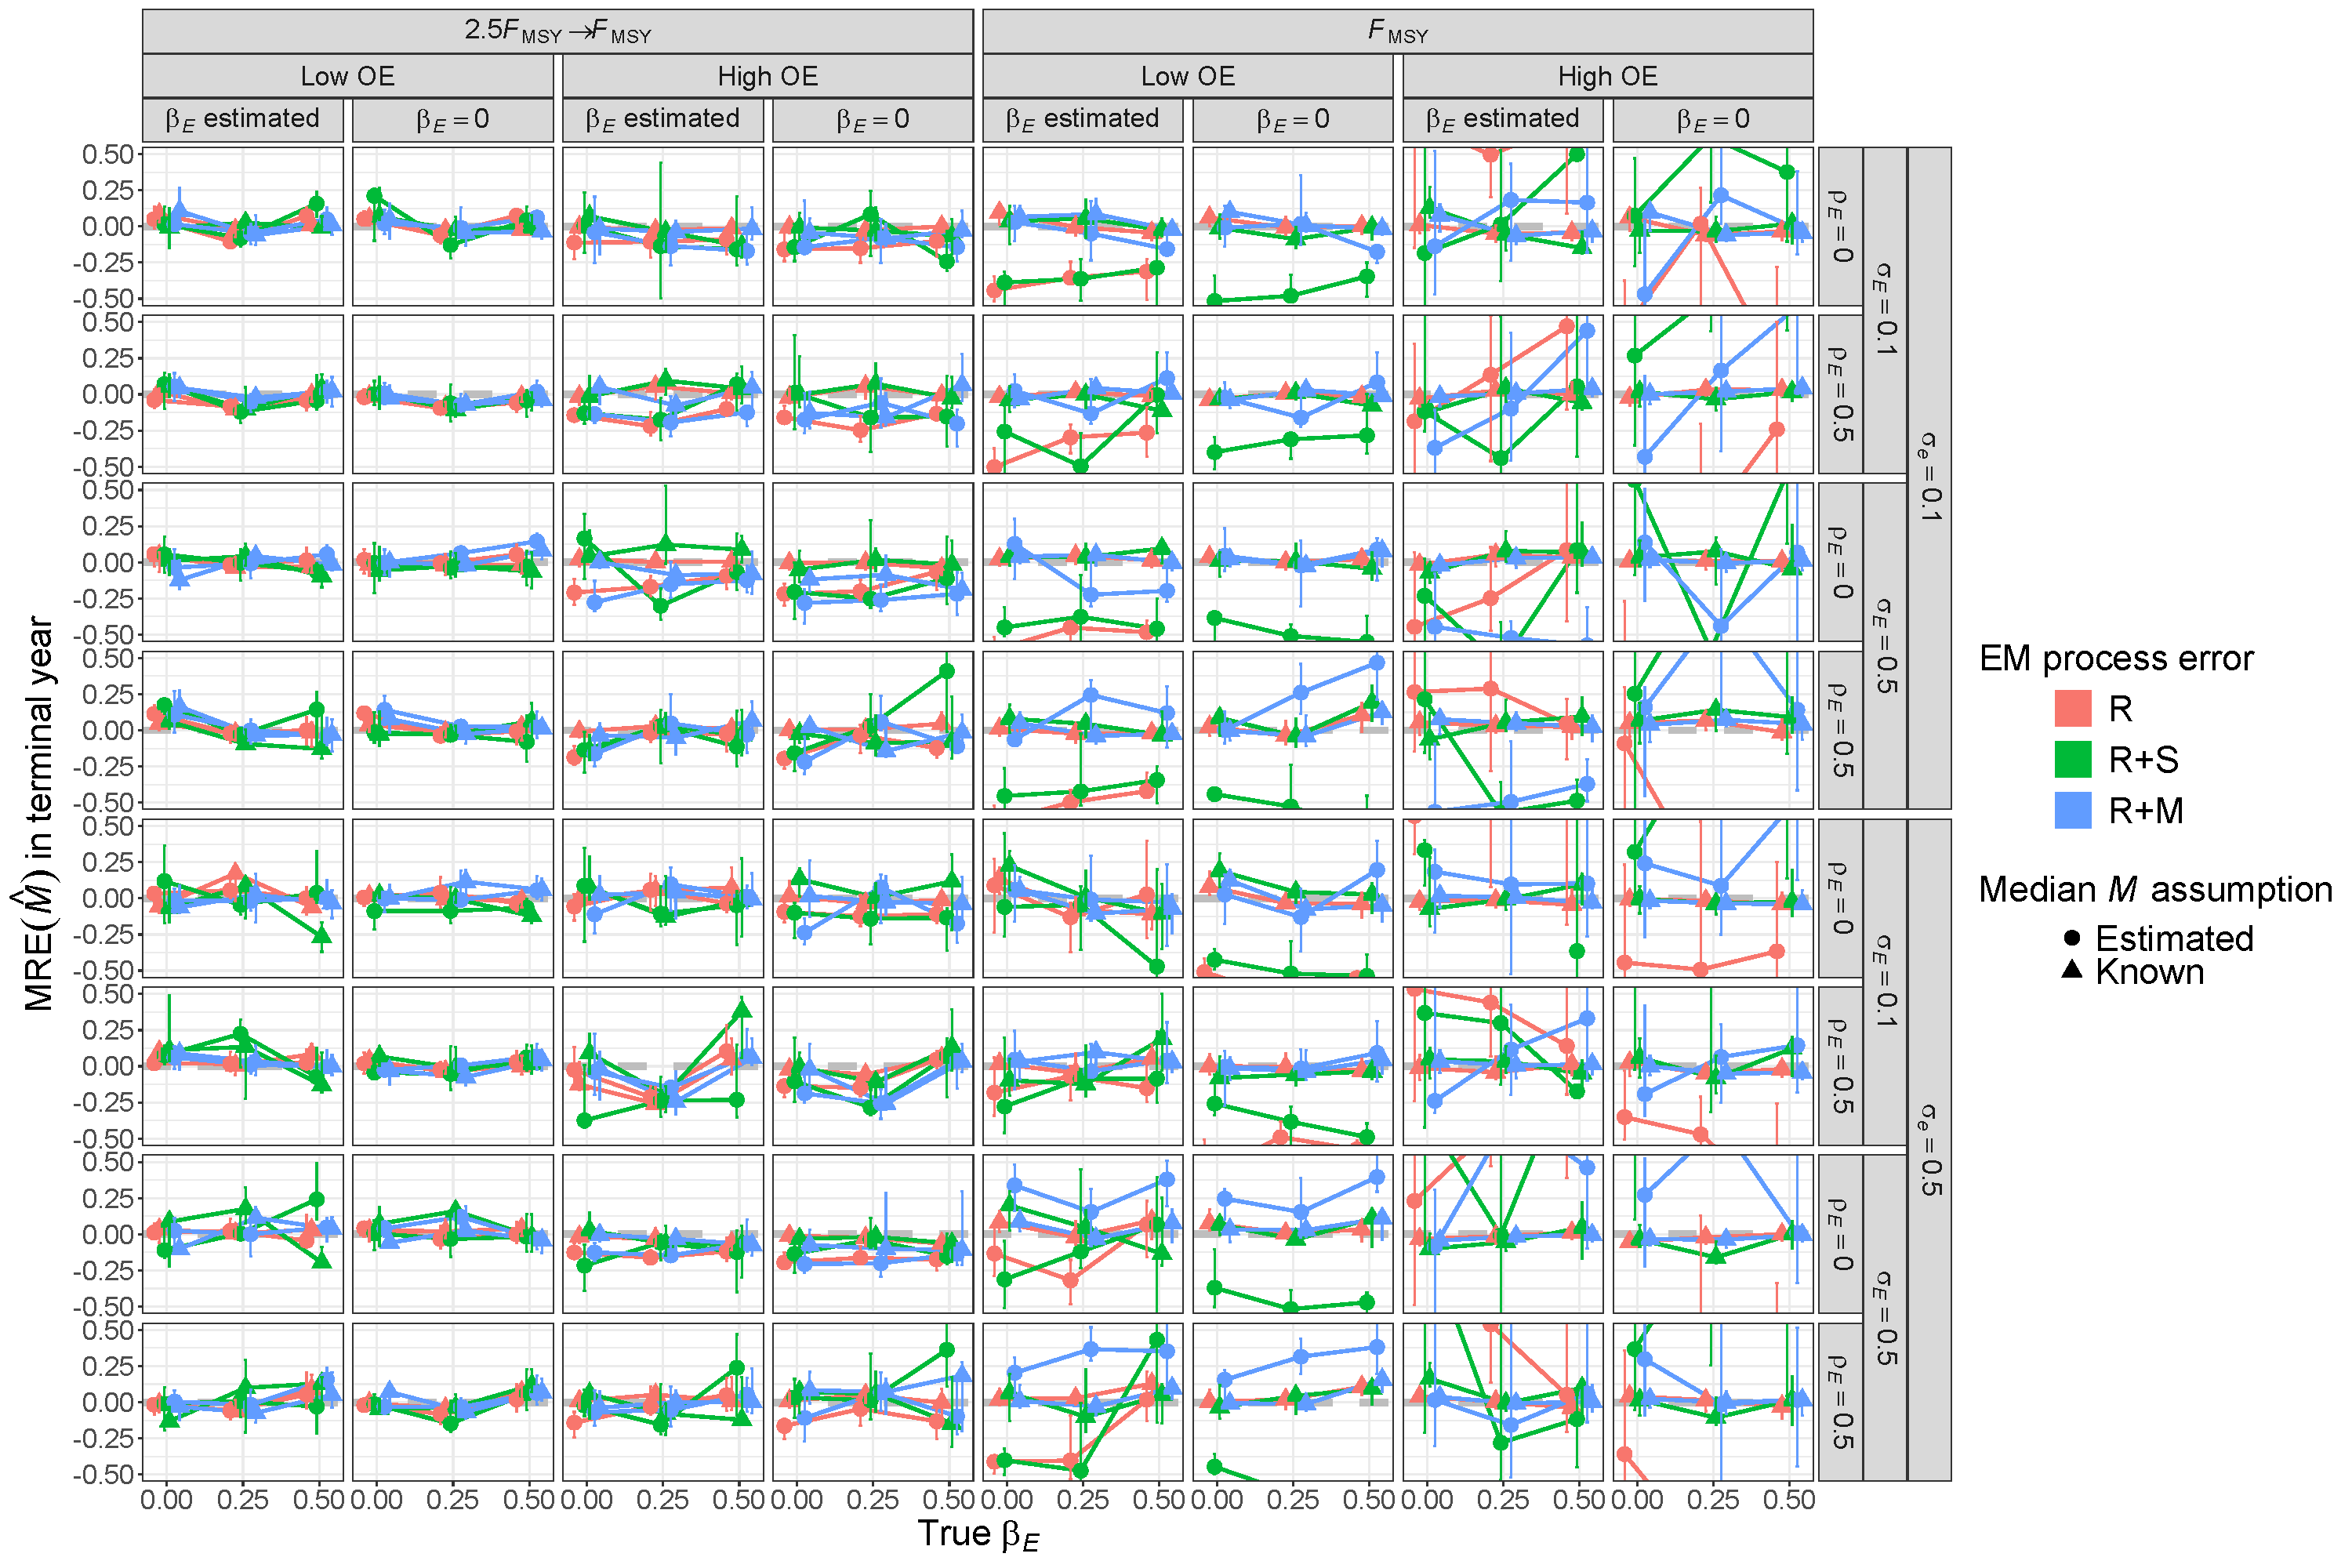
\includegraphics[height = \textheight]{terminal_year_M_bias_RMom}
%DIFDELCMD < %%%
\DIFdelendFL \DIFaddbeginFL 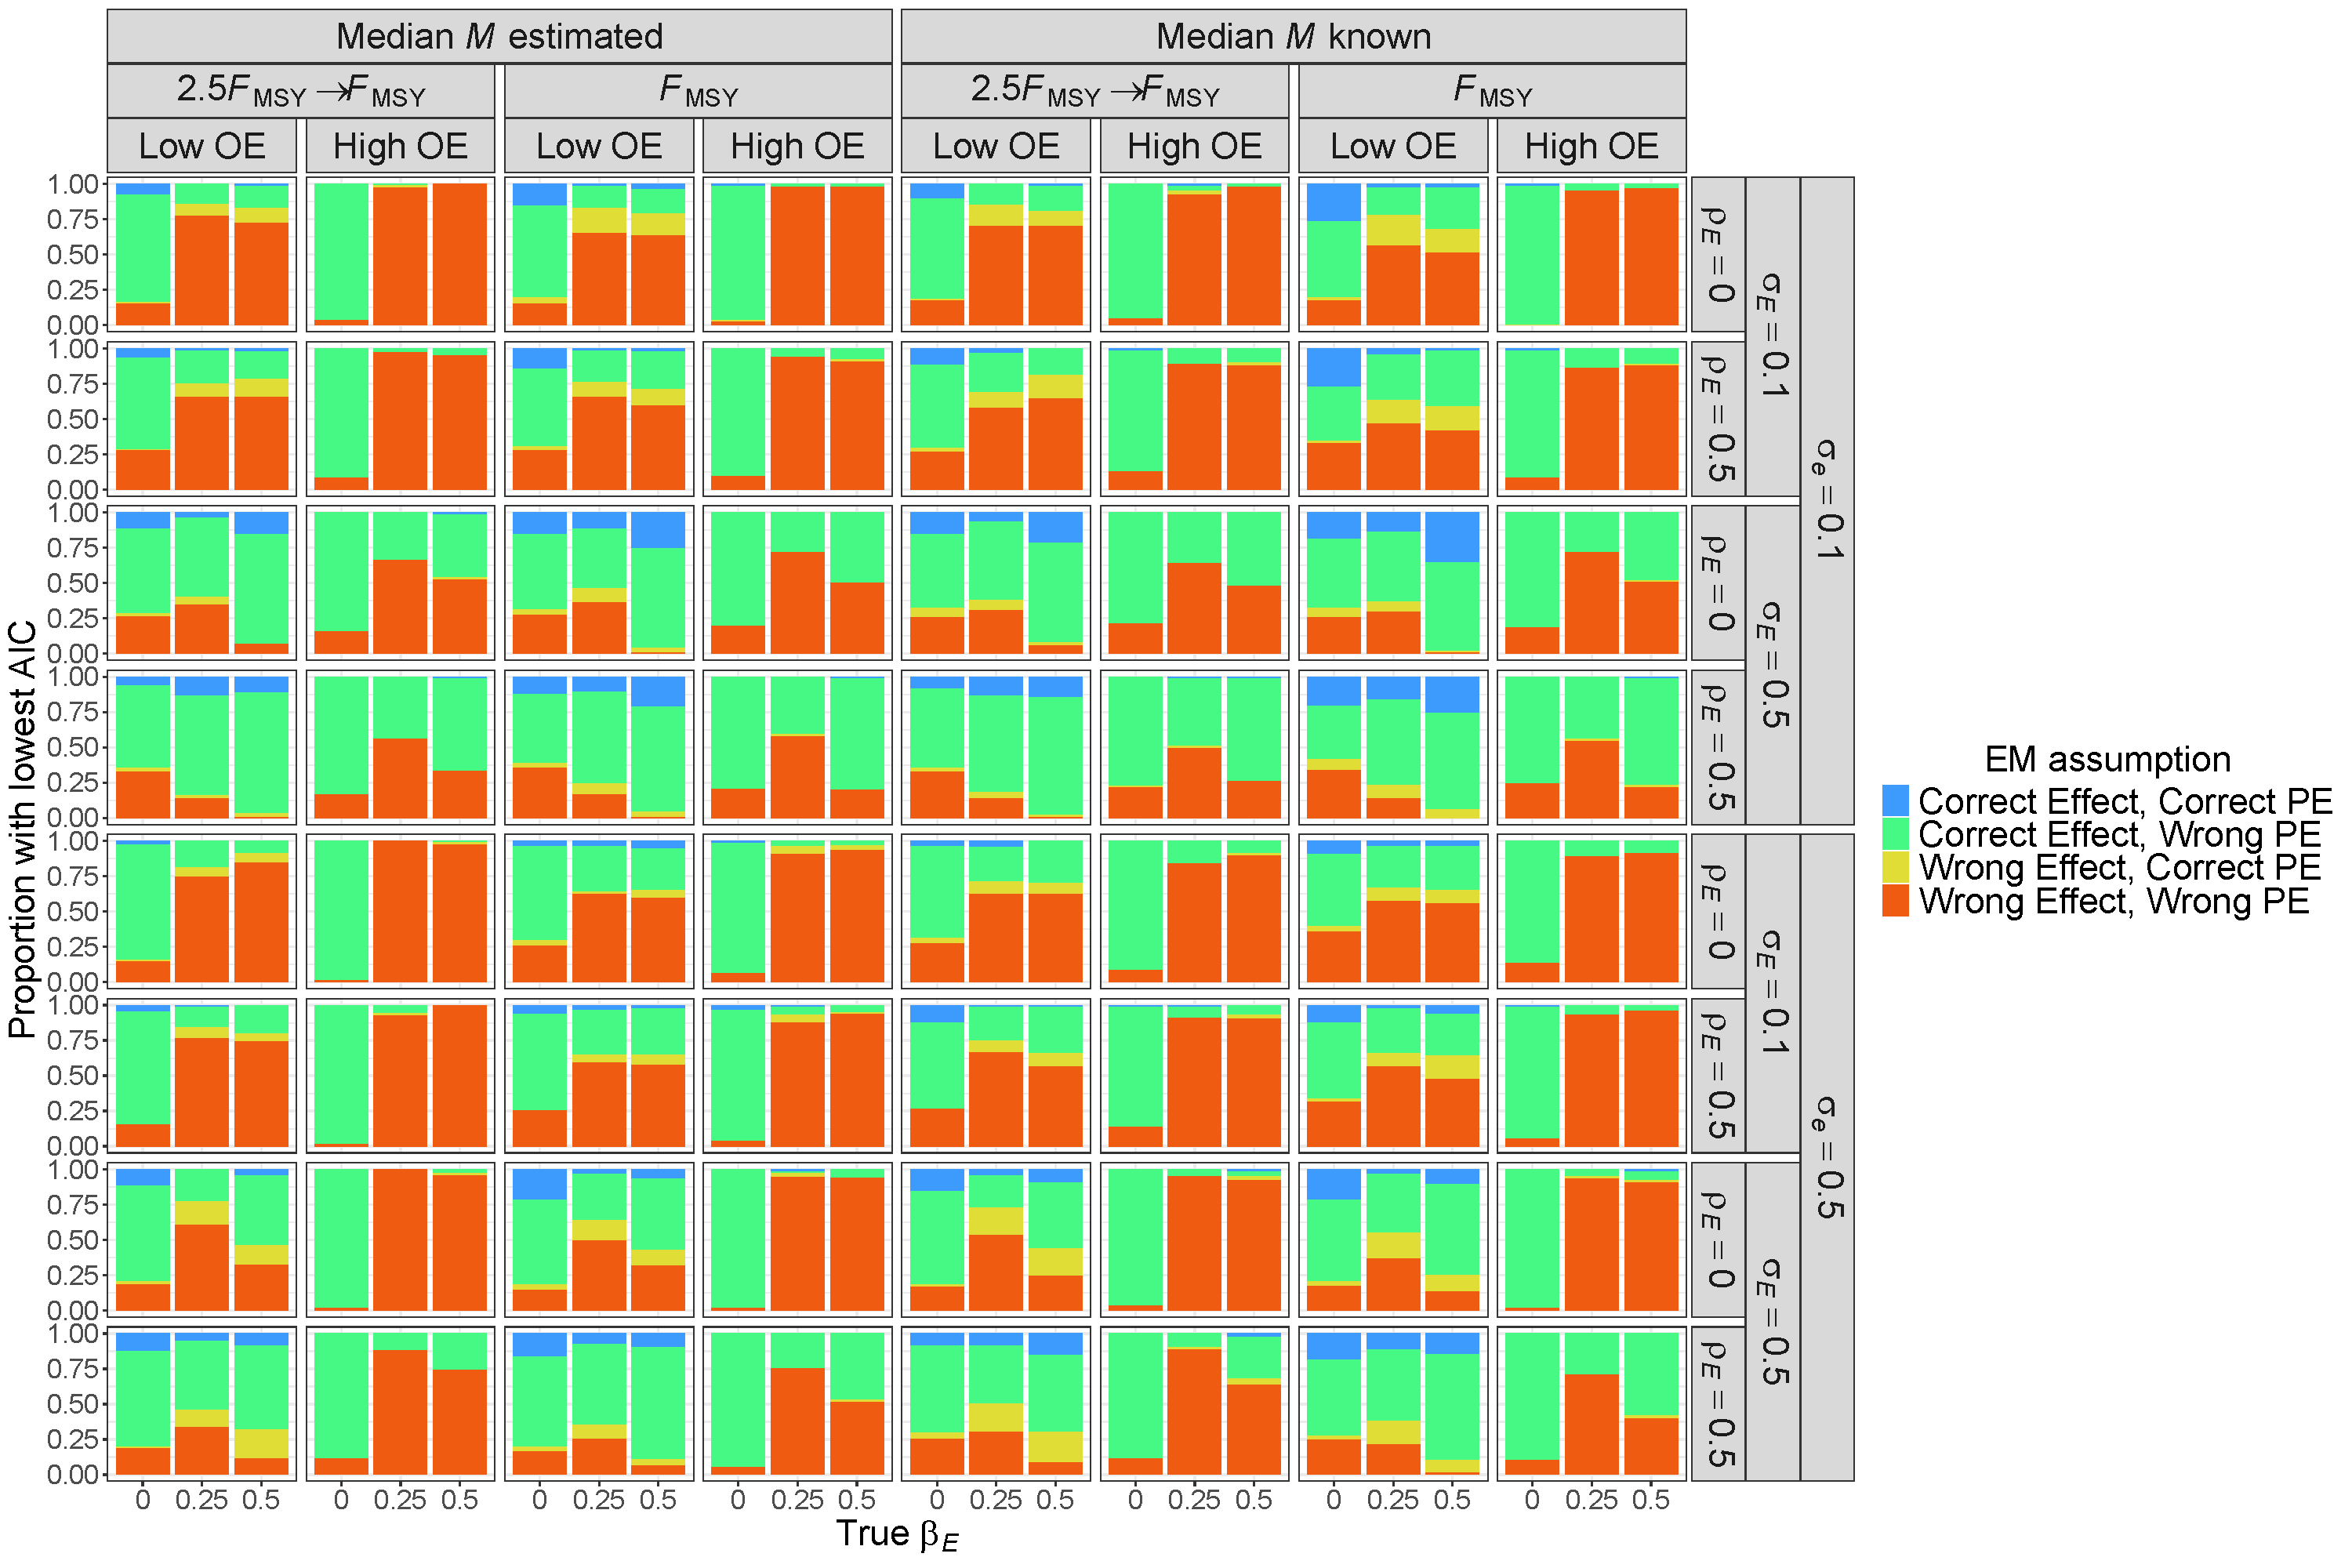
\includegraphics[height = \textheight]{aic_RMom}
\DIFaddendFL \end{center}
\caption{\DIFdelbeginFL \DIFdelFL{For }\DIFdelendFL \DIFaddbeginFL \DIFaddFL{Proportion of simulated data sets for }\DIFaddendFL R+M \DIFdelbeginFL \DIFdelFL{OMs, median relative error }\DIFdelendFL \DIFaddbeginFL \DIFaddFL{operating models where the estimating model type }\DIFaddendFL (\DIFdelbeginFL \DIFdelFL{MRE) of estimates of terminal year $M$ for EMs with alternative process error assumptions, }\DIFdelendFL treatment of \DIFaddbeginFL \DIFaddFL{environmental }\DIFaddendFL covariate \DIFdelbeginFL \DIFdelFL{effect ($\beta_E = 0$ or estimated), }\DIFdelendFL and \DIFdelbeginFL \DIFdelFL{treatment of median $M$ parameter ($\beta_M$ estimated or known}\DIFdelendFL \DIFaddbeginFL \DIFaddFL{assumed process error type}\DIFaddendFL ) \DIFaddbeginFL \DIFaddFL{had the lowest AIC}\DIFaddendFL .}\DIFdelbeginFL %DIFDELCMD < \label{terminal_M_bias_RMom}
%DIFDELCMD < %%%
\DIFdelendFL \DIFaddbeginFL \label{aic_RMom}
\DIFaddendFL \end{figure}
\end{landscape}

\DIFdelbegin \subsection*{\DIFdel{Terminal year natural mortality accuracy}}%DIFAUXCMD
%DIFDELCMD < \label{terminal-year-natural-mortality-accuracy}
%DIFDELCMD < %%%
\addcontentsline{toc}{subsection}{\DIFdel{Terminal year natural mortality accuracy}}
%DIFAUXCMD
%DIFDELCMD < 

%DIFDELCMD < %%%
\DIFdelend \begin{landscape}
\begin{figure}
\begin{center}
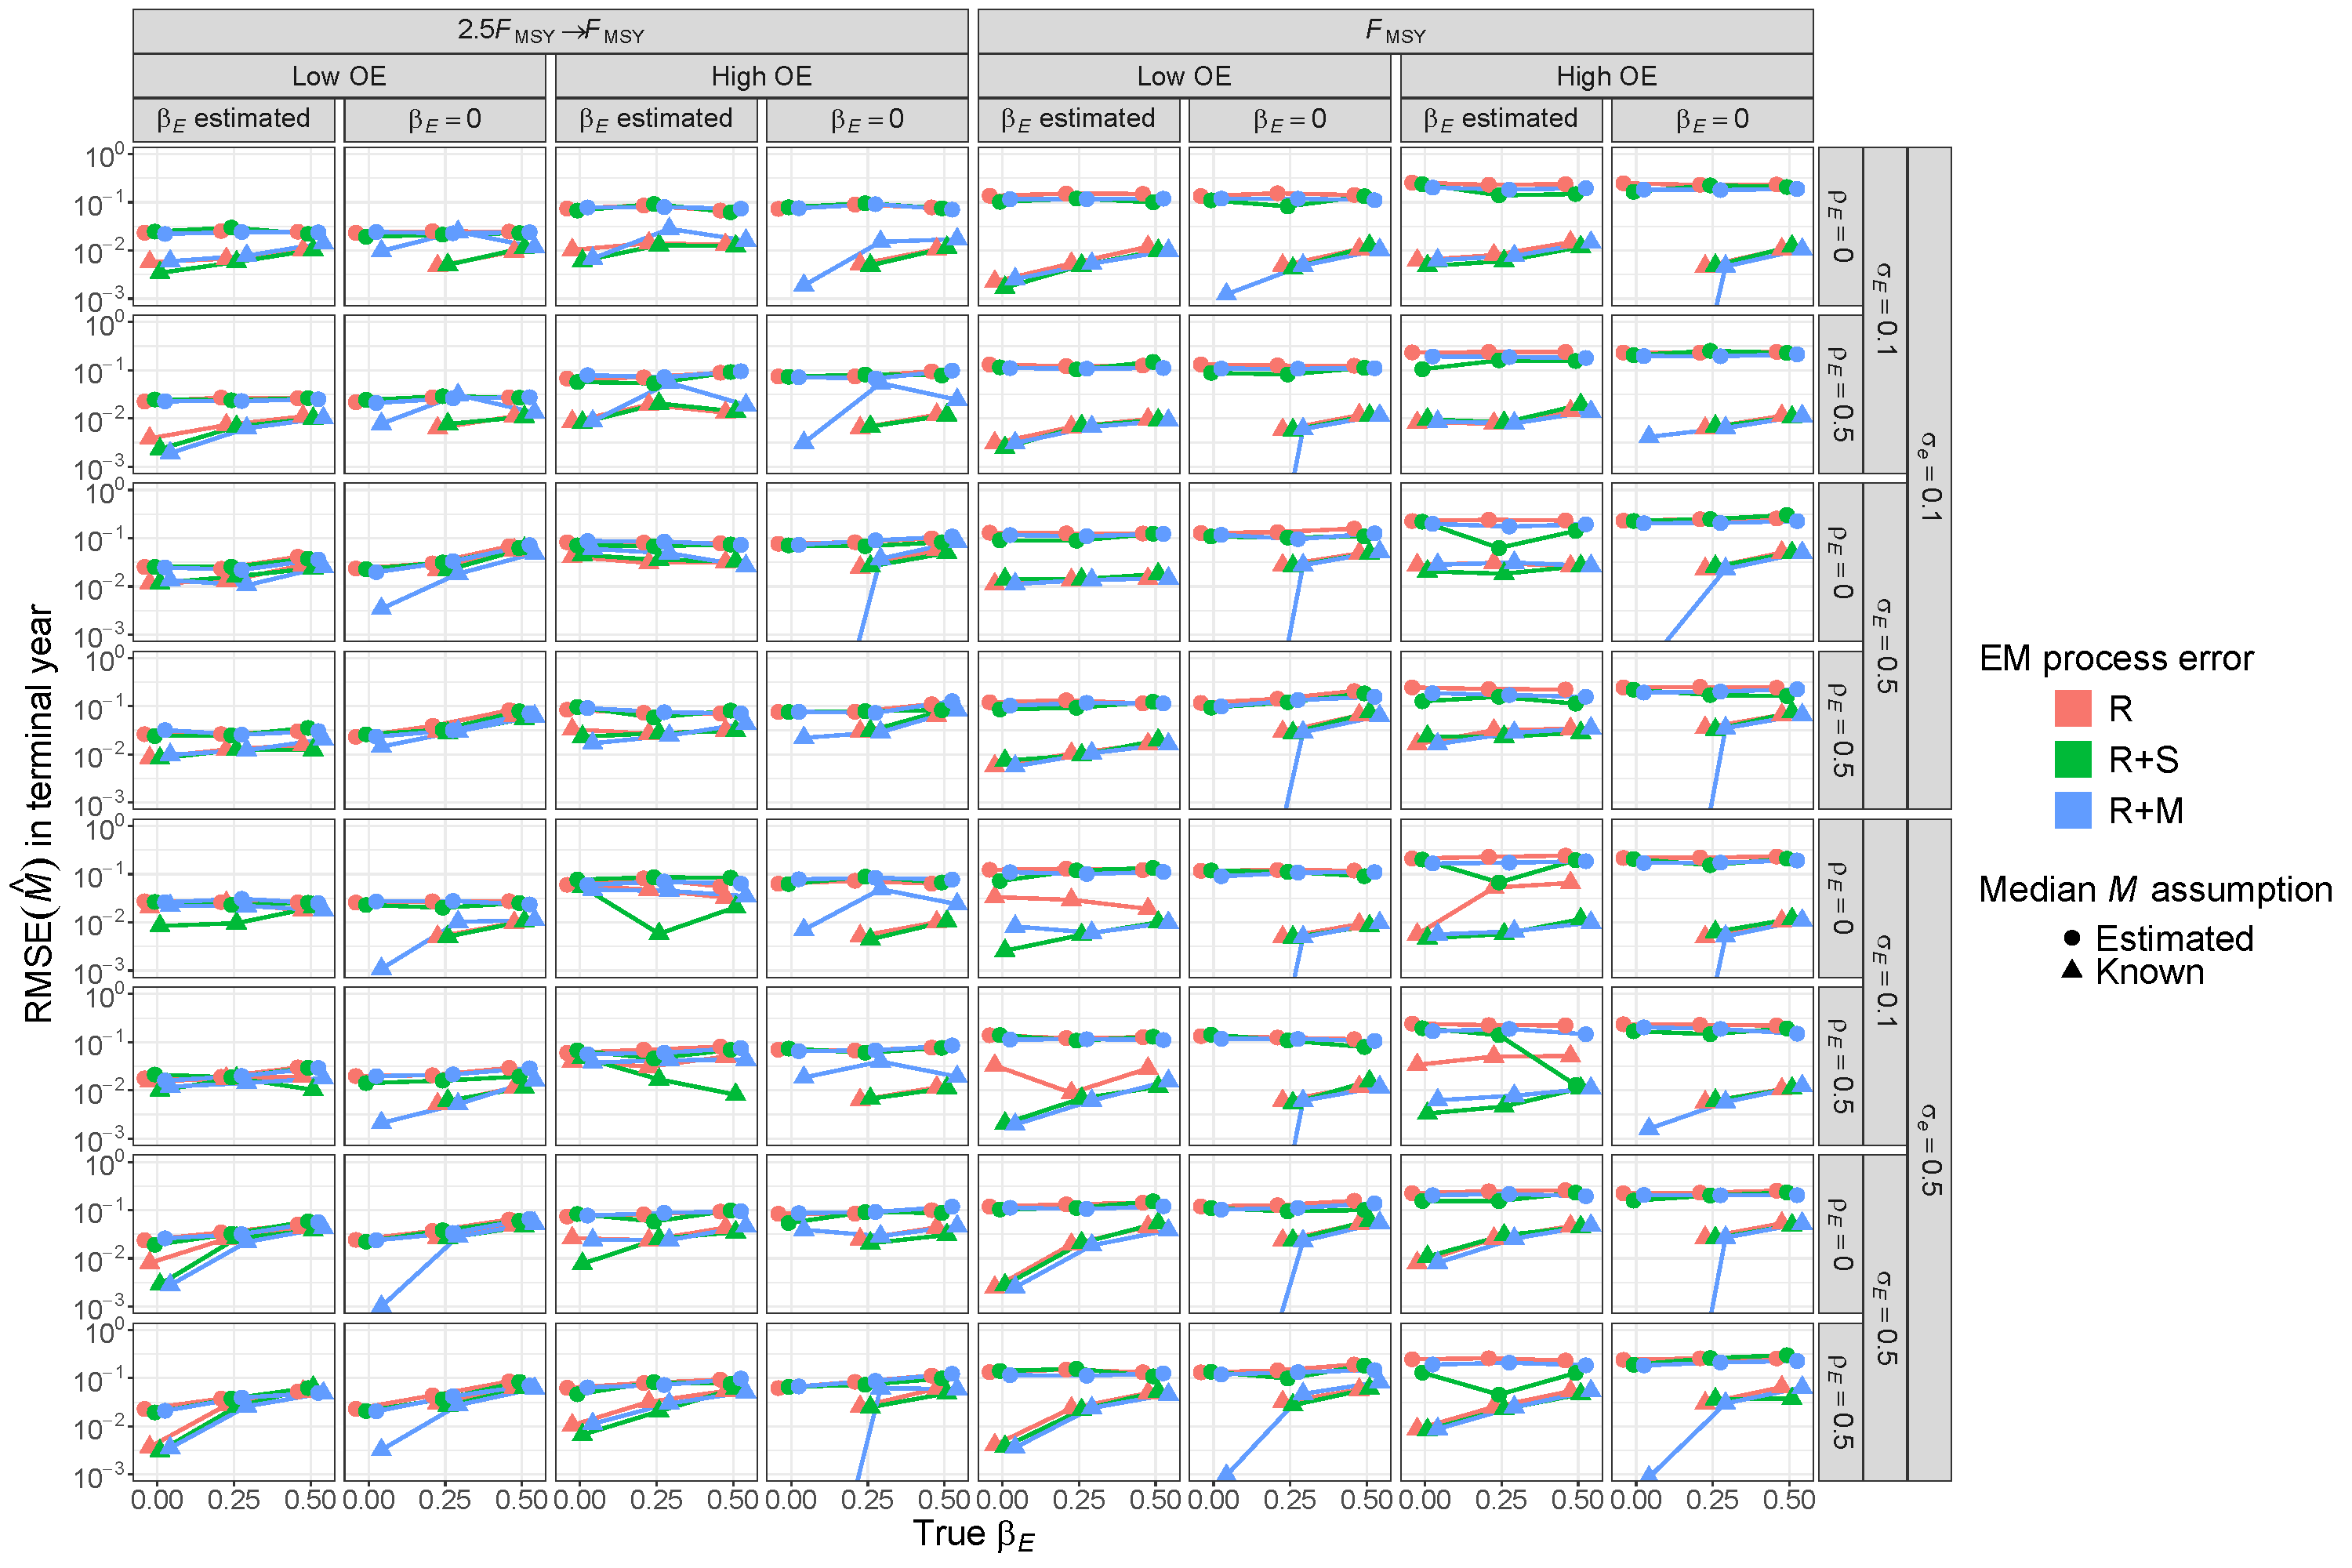
\includegraphics[height = \textheight]{terminal_year_M_rmse_Rom}
\end{center}
\caption{For R \DIFdelbeginFL \DIFdelFL{OMs}\DIFdelendFL \DIFaddbeginFL \DIFaddFL{operating models}\DIFaddendFL , RMSE of estimates of terminal year $M$ for \DIFdelbeginFL \DIFdelFL{EMs }\DIFdelendFL \DIFaddbeginFL \DIFaddFL{estimating models }\DIFaddendFL with alternative process error assumptions, treatment of covariate effect ($\beta_E = 0$ or estimated), and treatment of median $M$ parameter ($\beta_M$ estimated or known).}\label{terminal_M_rmse_Rom}
\end{figure}
\end{landscape}

\begin{landscape}
\begin{figure}
\begin{center}
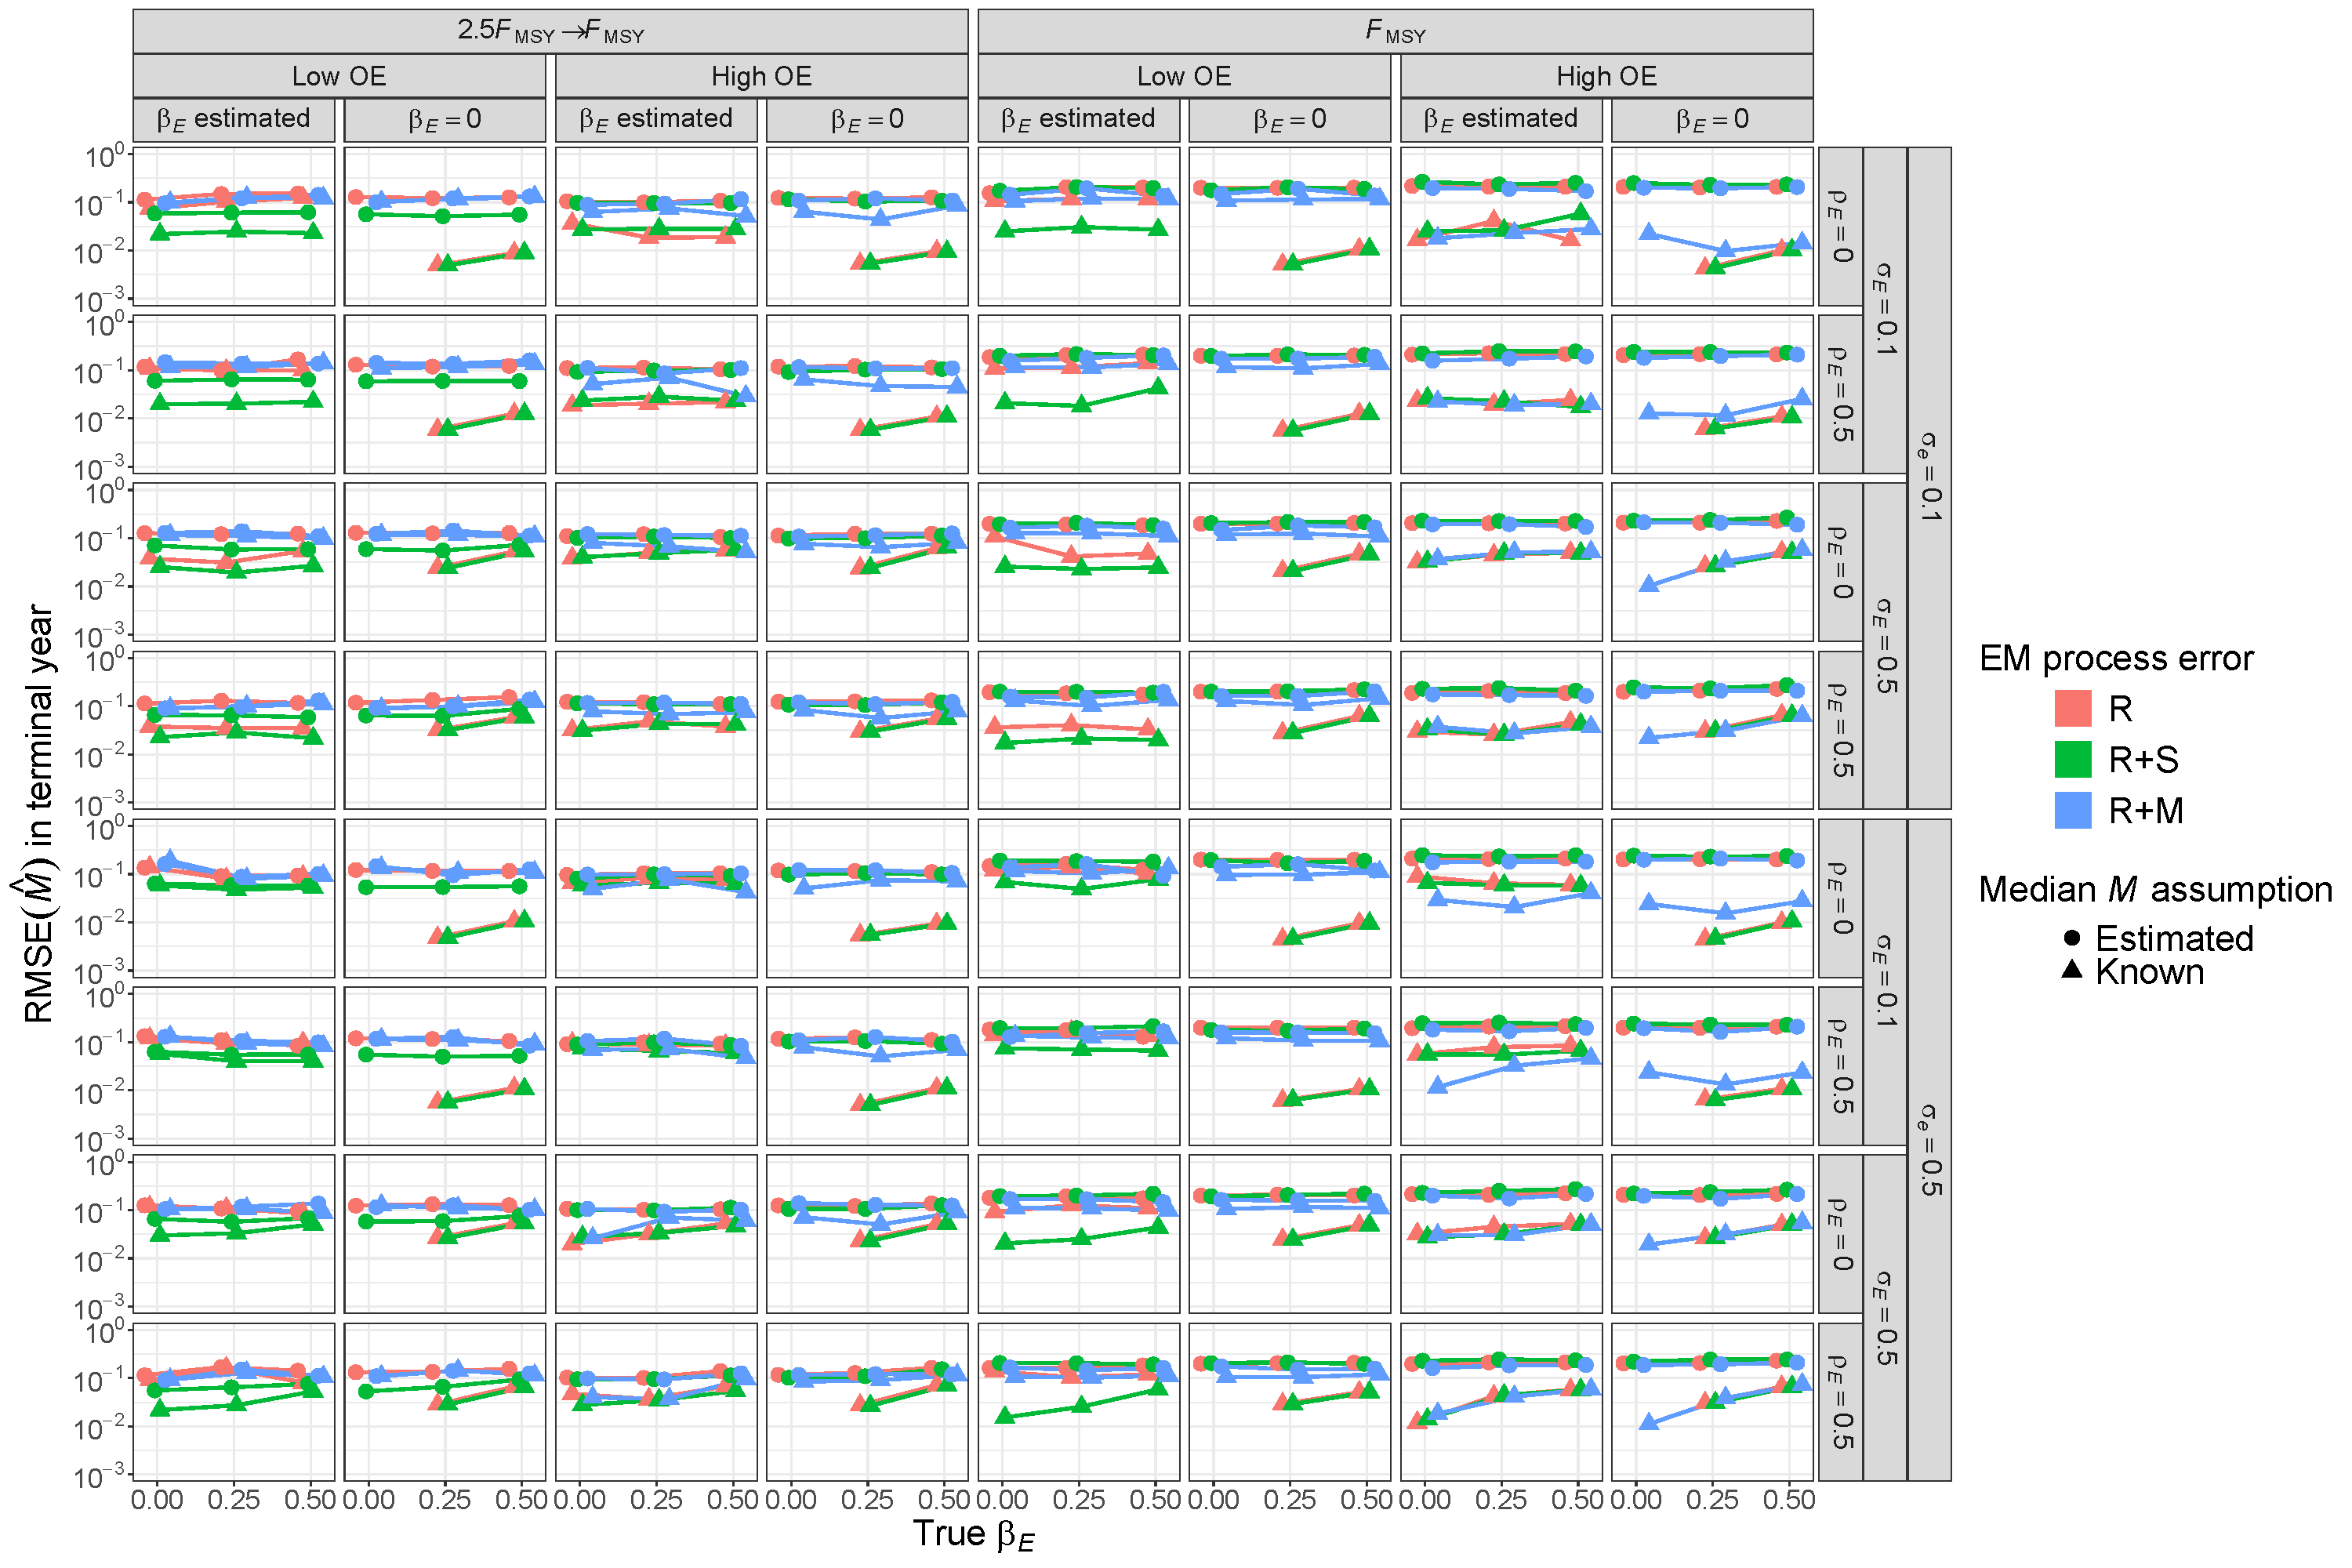
\includegraphics[height = \textheight]{terminal_year_M_rmse_RSom}
\end{center}
\caption{For R+S \DIFdelbeginFL \DIFdelFL{OMs}\DIFdelendFL \DIFaddbeginFL \DIFaddFL{operating models}\DIFaddendFL , RMSE of estimates of terminal year $M$ for \DIFdelbeginFL \DIFdelFL{EMs }\DIFdelendFL \DIFaddbeginFL \DIFaddFL{estimating models }\DIFaddendFL with alternative process error assumptions, treatment of covariate effect ($\beta_E = 0$ or estimated), and treatment of median $M$ parameter ($\beta_M$ estimated or known).}\label{terminal_M_rmse_RSom}
\end{figure}
\end{landscape}

\begin{landscape}
\begin{figure}
\begin{center}
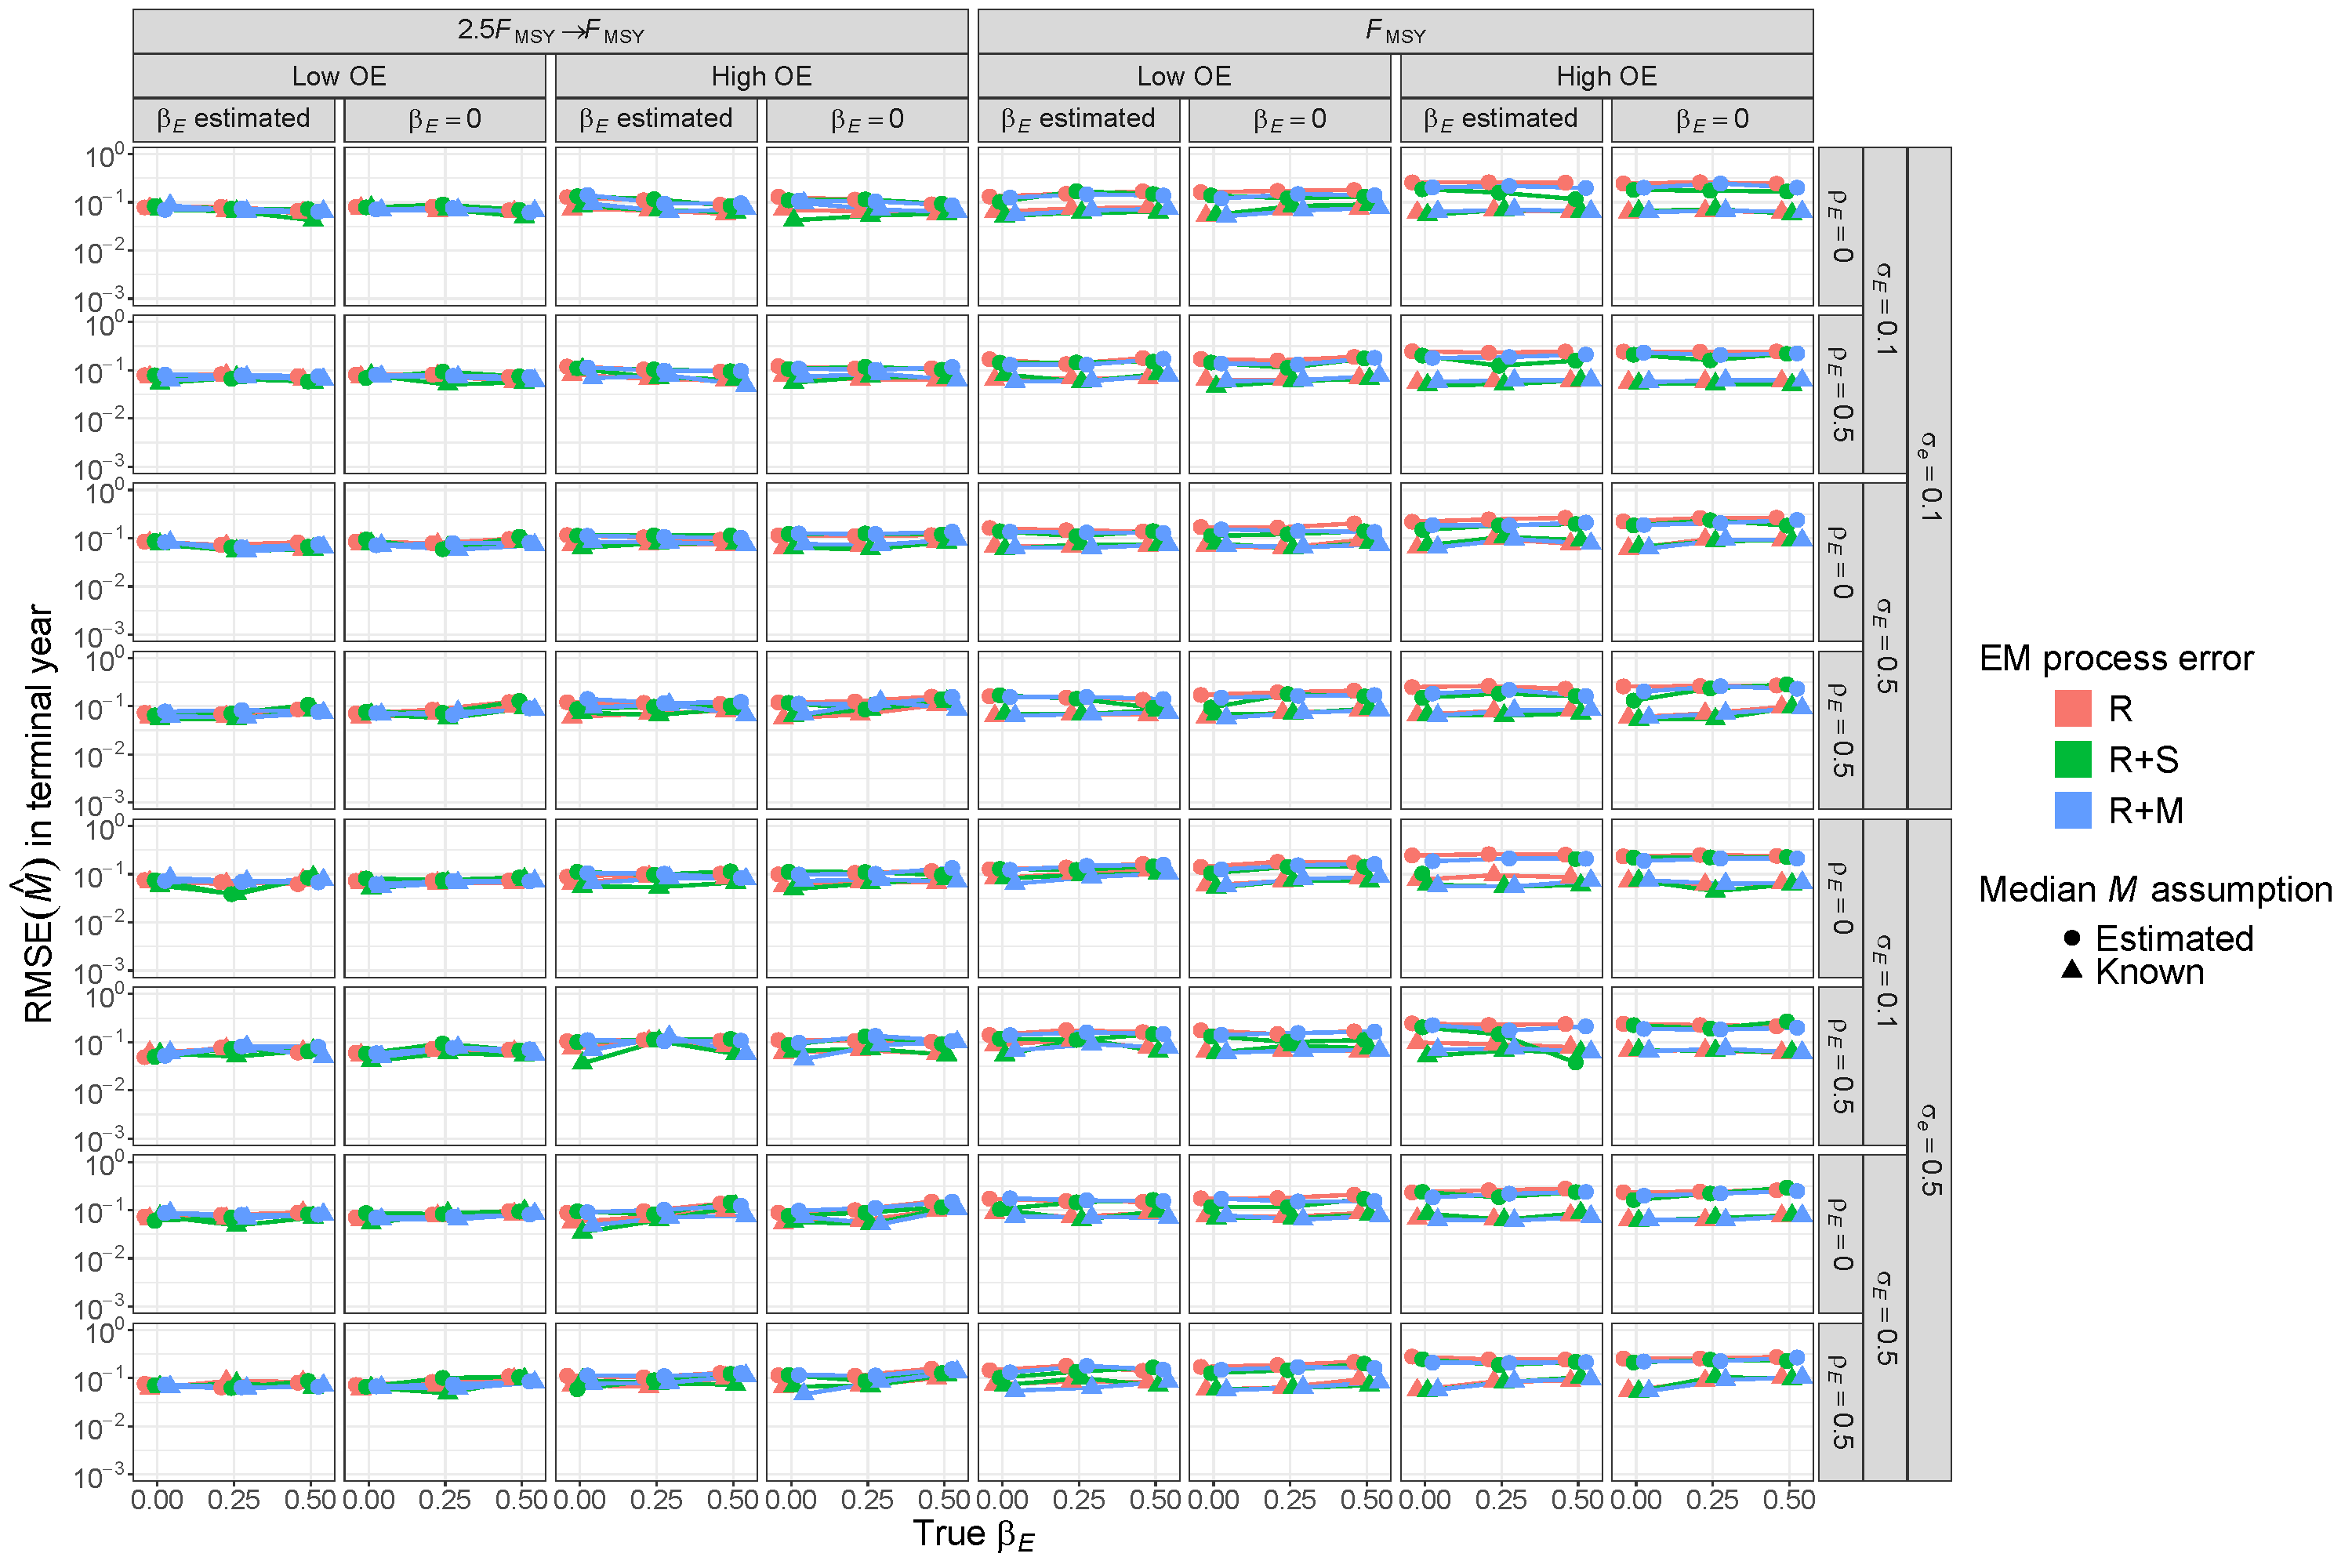
\includegraphics[height = \textheight]{terminal_year_M_rmse_RMom}
\end{center}
\caption{For R+M \DIFdelbeginFL \DIFdelFL{OMs}\DIFdelendFL \DIFaddbeginFL \DIFaddFL{operating models}\DIFaddendFL , RMSE of estimates of terminal year $M$ for \DIFdelbeginFL \DIFdelFL{EMs }\DIFdelendFL \DIFaddbeginFL \DIFaddFL{estimating models }\DIFaddendFL with alternative process error assumptions, treatment of covariate effect ($\beta_E = 0$ or estimated), and treatment of median $M$ parameter ($\beta_M$ estimated or known).}\label{terminal_M_rmse_RMom}
\end{figure}
\end{landscape}

\begin{landscape}
\begin{figure}
\begin{center}
\DIFdelbeginFL %DIFDELCMD < 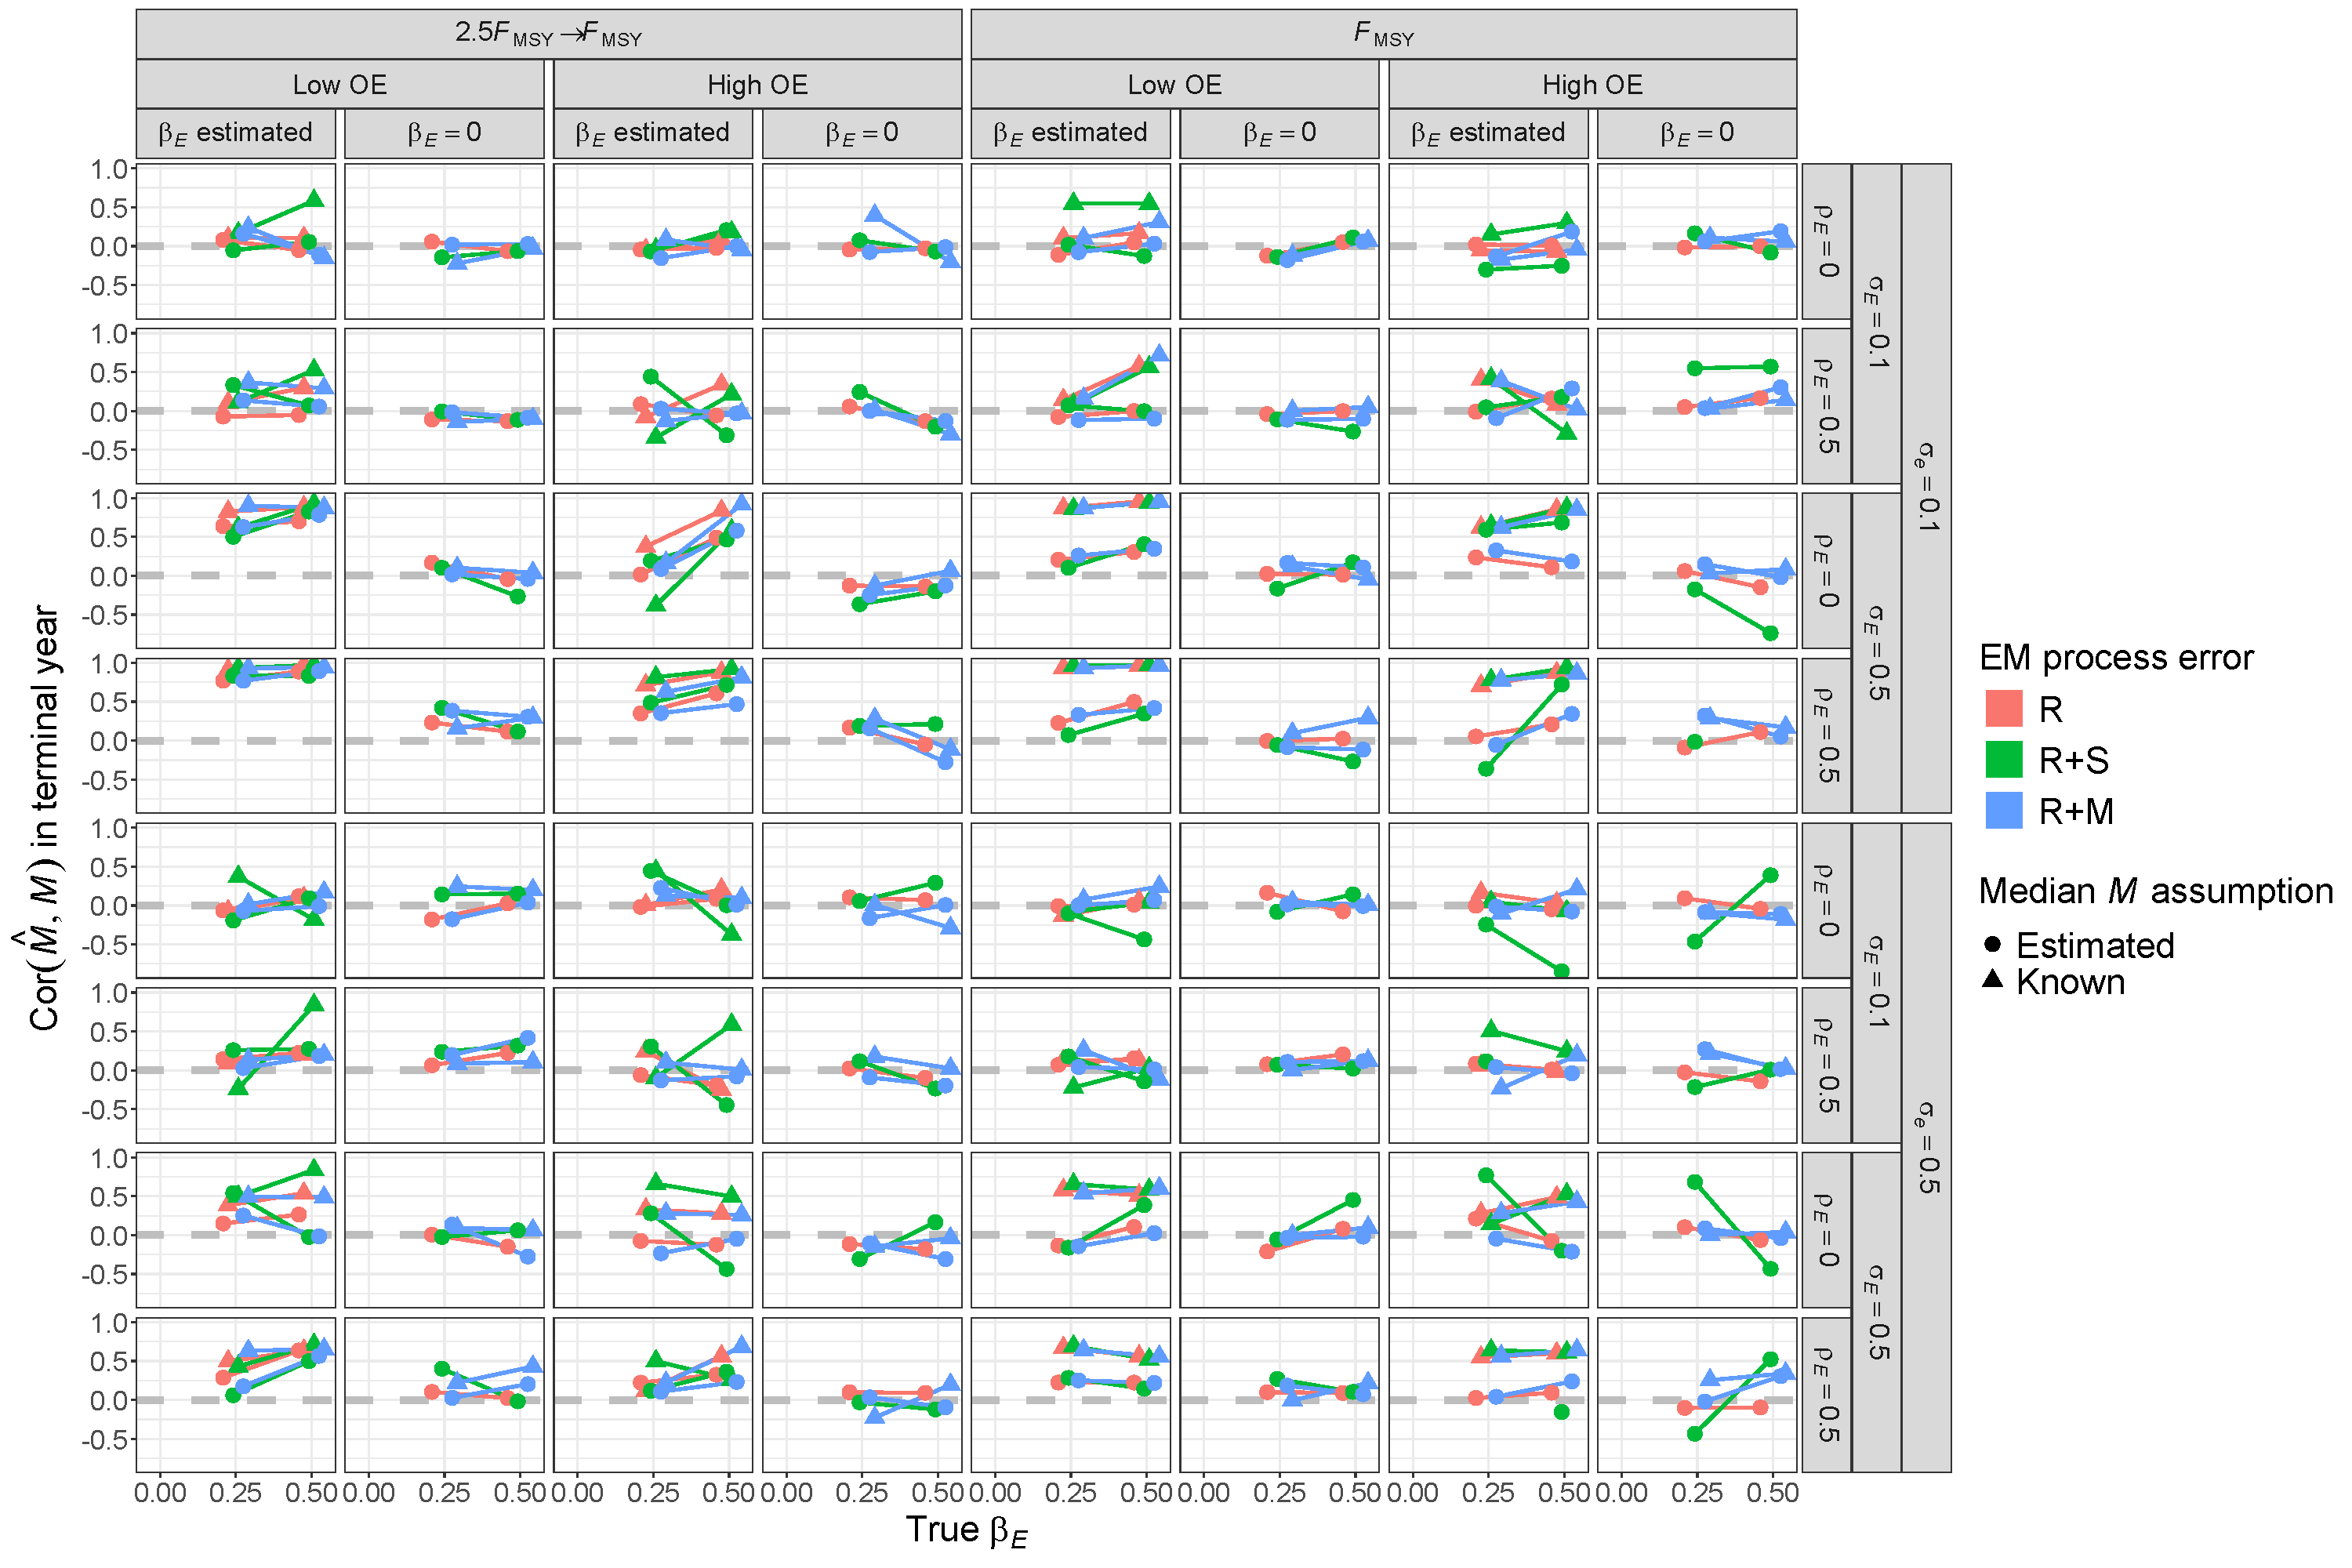
\includegraphics[height = \textheight]{terminal_year_M_corr_Rom}
%DIFDELCMD < \end{center}
%DIFDELCMD < %%%
%DIFDELCMD < \caption{%
{%DIFAUXCMD
\DIFdelFL{For R OMs, correlation of estimates and true values of terminal year $M$ for EMs with alternative process error assumptions, treatment of covariate effect ($\beta_E = 0$ or estimated), and treatment of median $M$ parameter ($\beta_M$ estimated or known).}}%DIFAUXCMD
%DIFDELCMD < \label{terminal_M_corr_Rom}
%DIFDELCMD < \end{figure}
%DIFDELCMD < \end{landscape}
%DIFDELCMD < 

%DIFDELCMD < \begin{landscape}
%DIFDELCMD < \begin{figure}
%DIFDELCMD < \begin{center}
%DIFDELCMD < 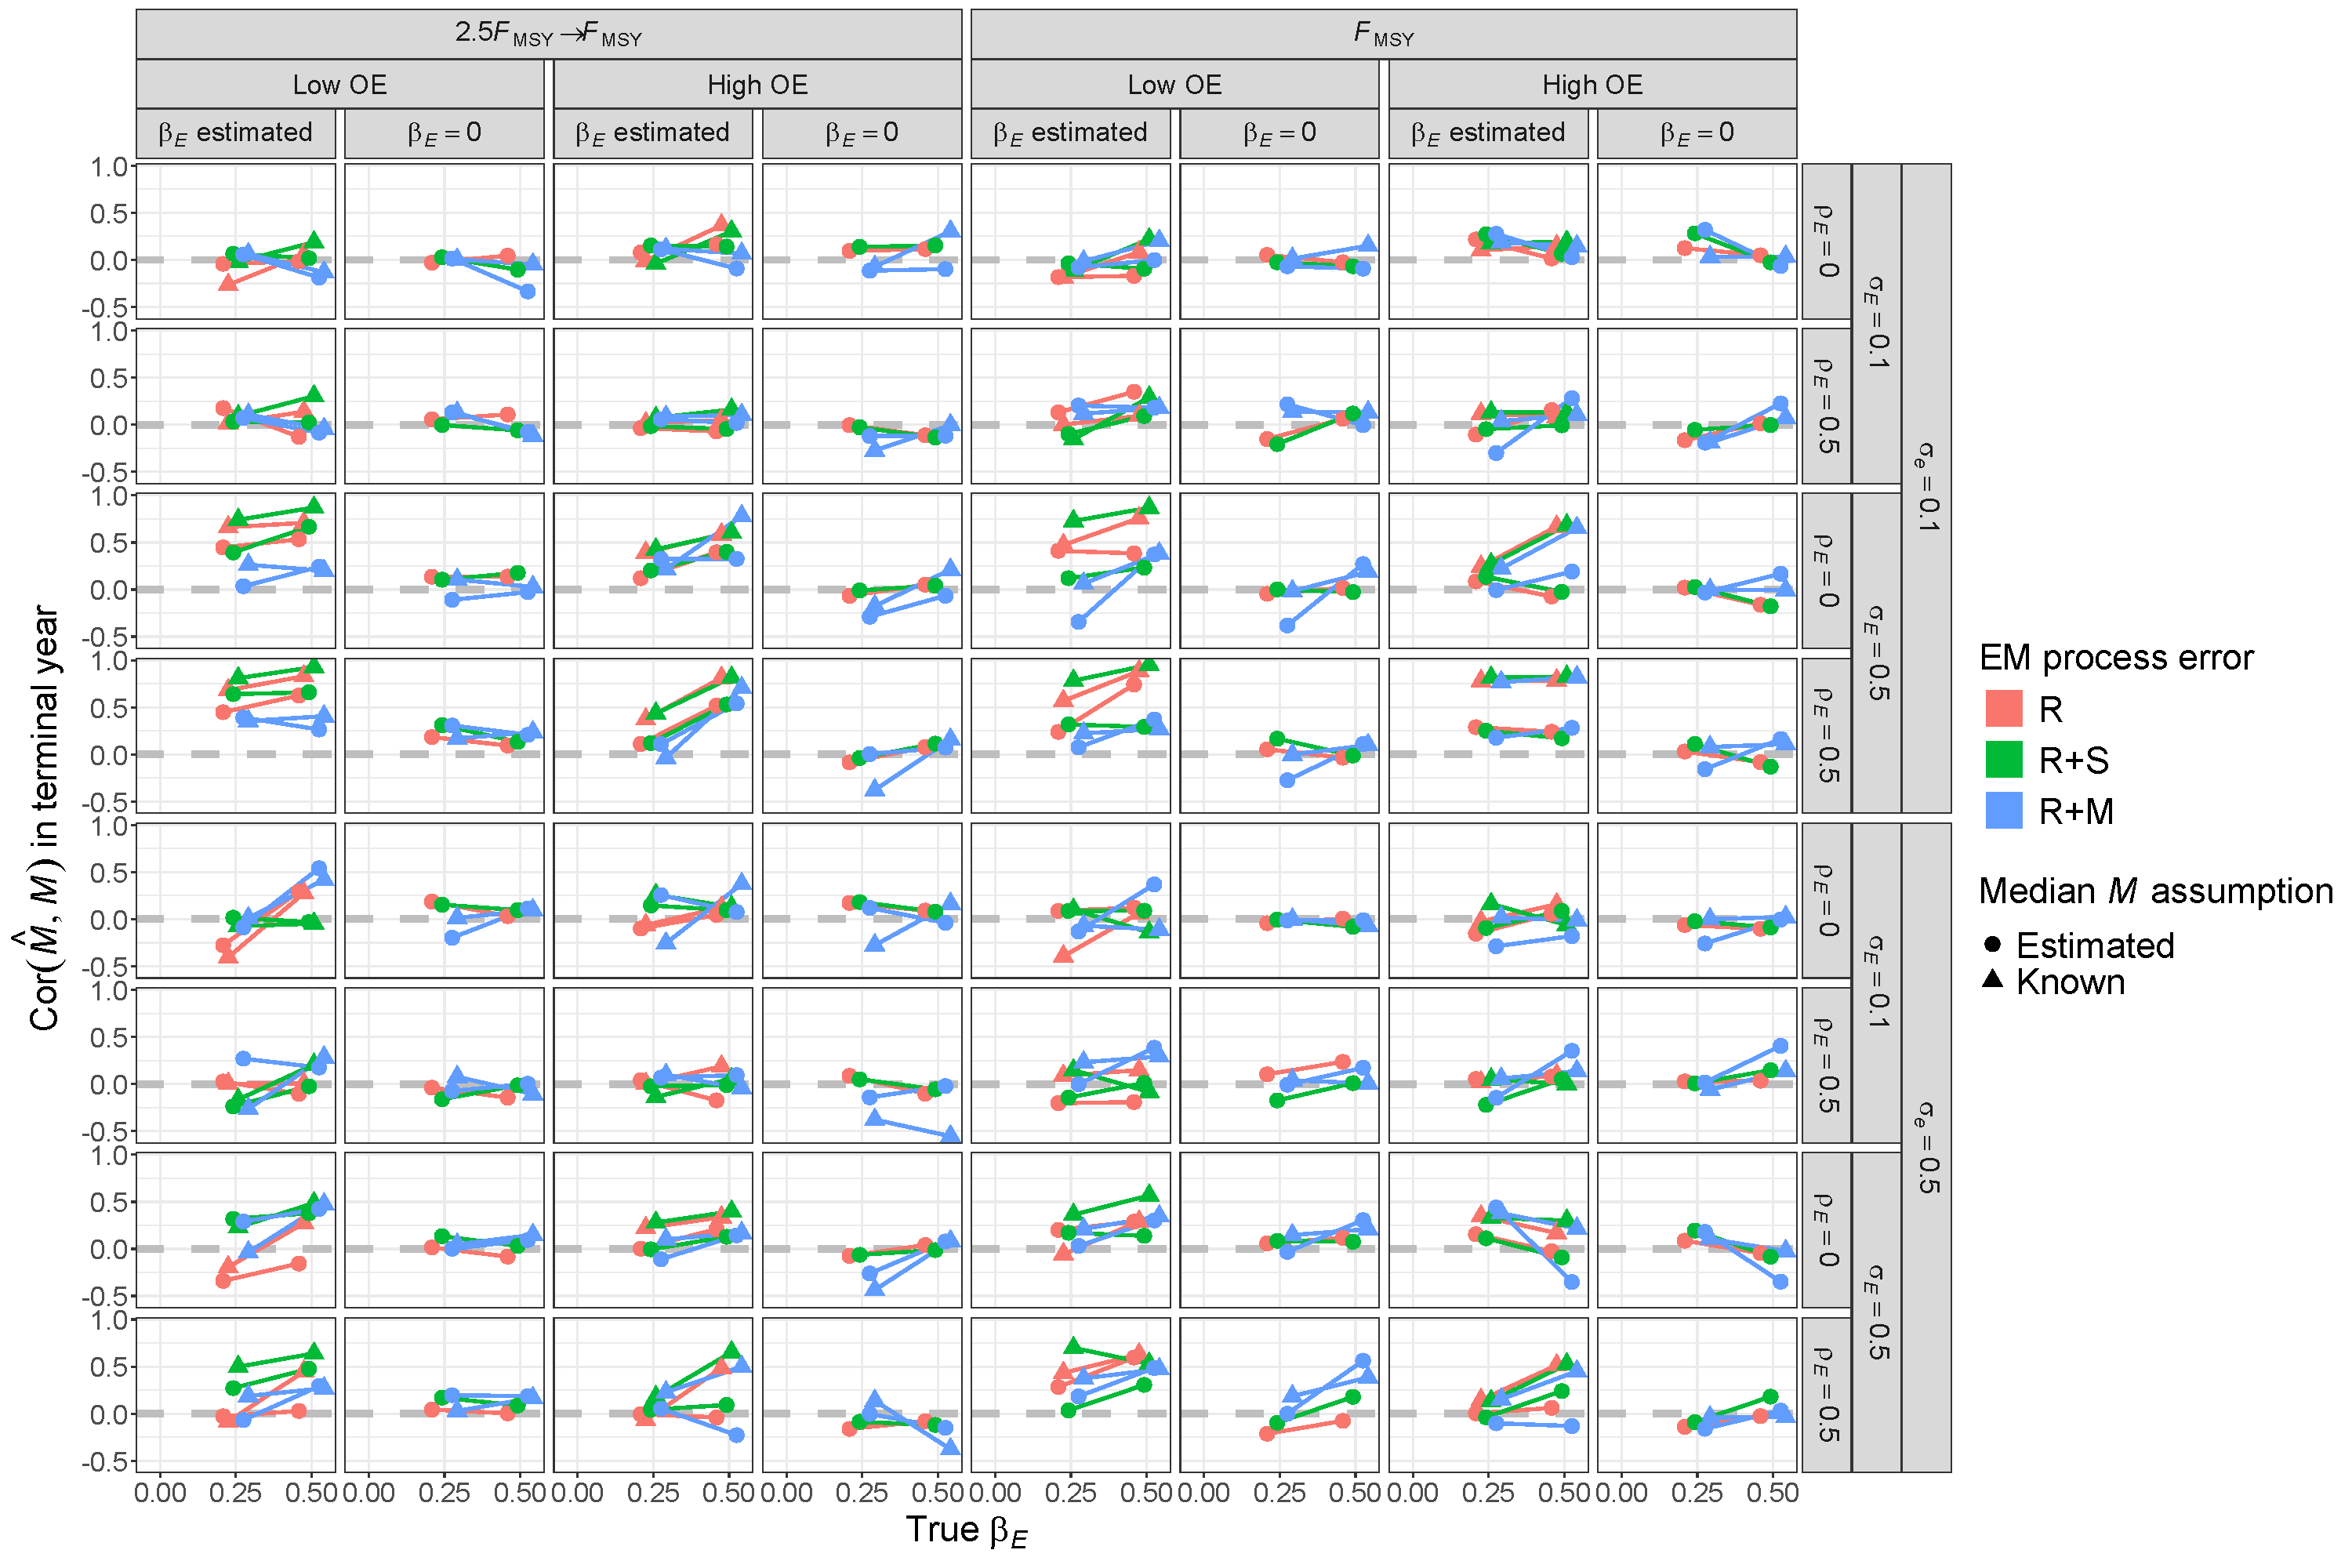
\includegraphics[height = \textheight]{terminal_year_M_corr_RSom}
%DIFDELCMD < \end{center}
%DIFDELCMD < %%%
%DIFDELCMD < \caption{%
{%DIFAUXCMD
\DIFdelFL{For R+S OMs, correlation of estimates and true values of terminal year $M$ for EMs with alternative process error assumptions, treatment of covariate effect ($\beta_E = 0$ or estimated), and treatment of median $M$ parameter ($\beta_M$ estimated or known).}}%DIFAUXCMD
%DIFDELCMD < \label{terminal_M_corr_RSom}
%DIFDELCMD < \end{figure}
%DIFDELCMD < \end{landscape}
%DIFDELCMD < 

%DIFDELCMD < \begin{landscape}
%DIFDELCMD < \begin{figure}
%DIFDELCMD < \begin{center}
%DIFDELCMD < 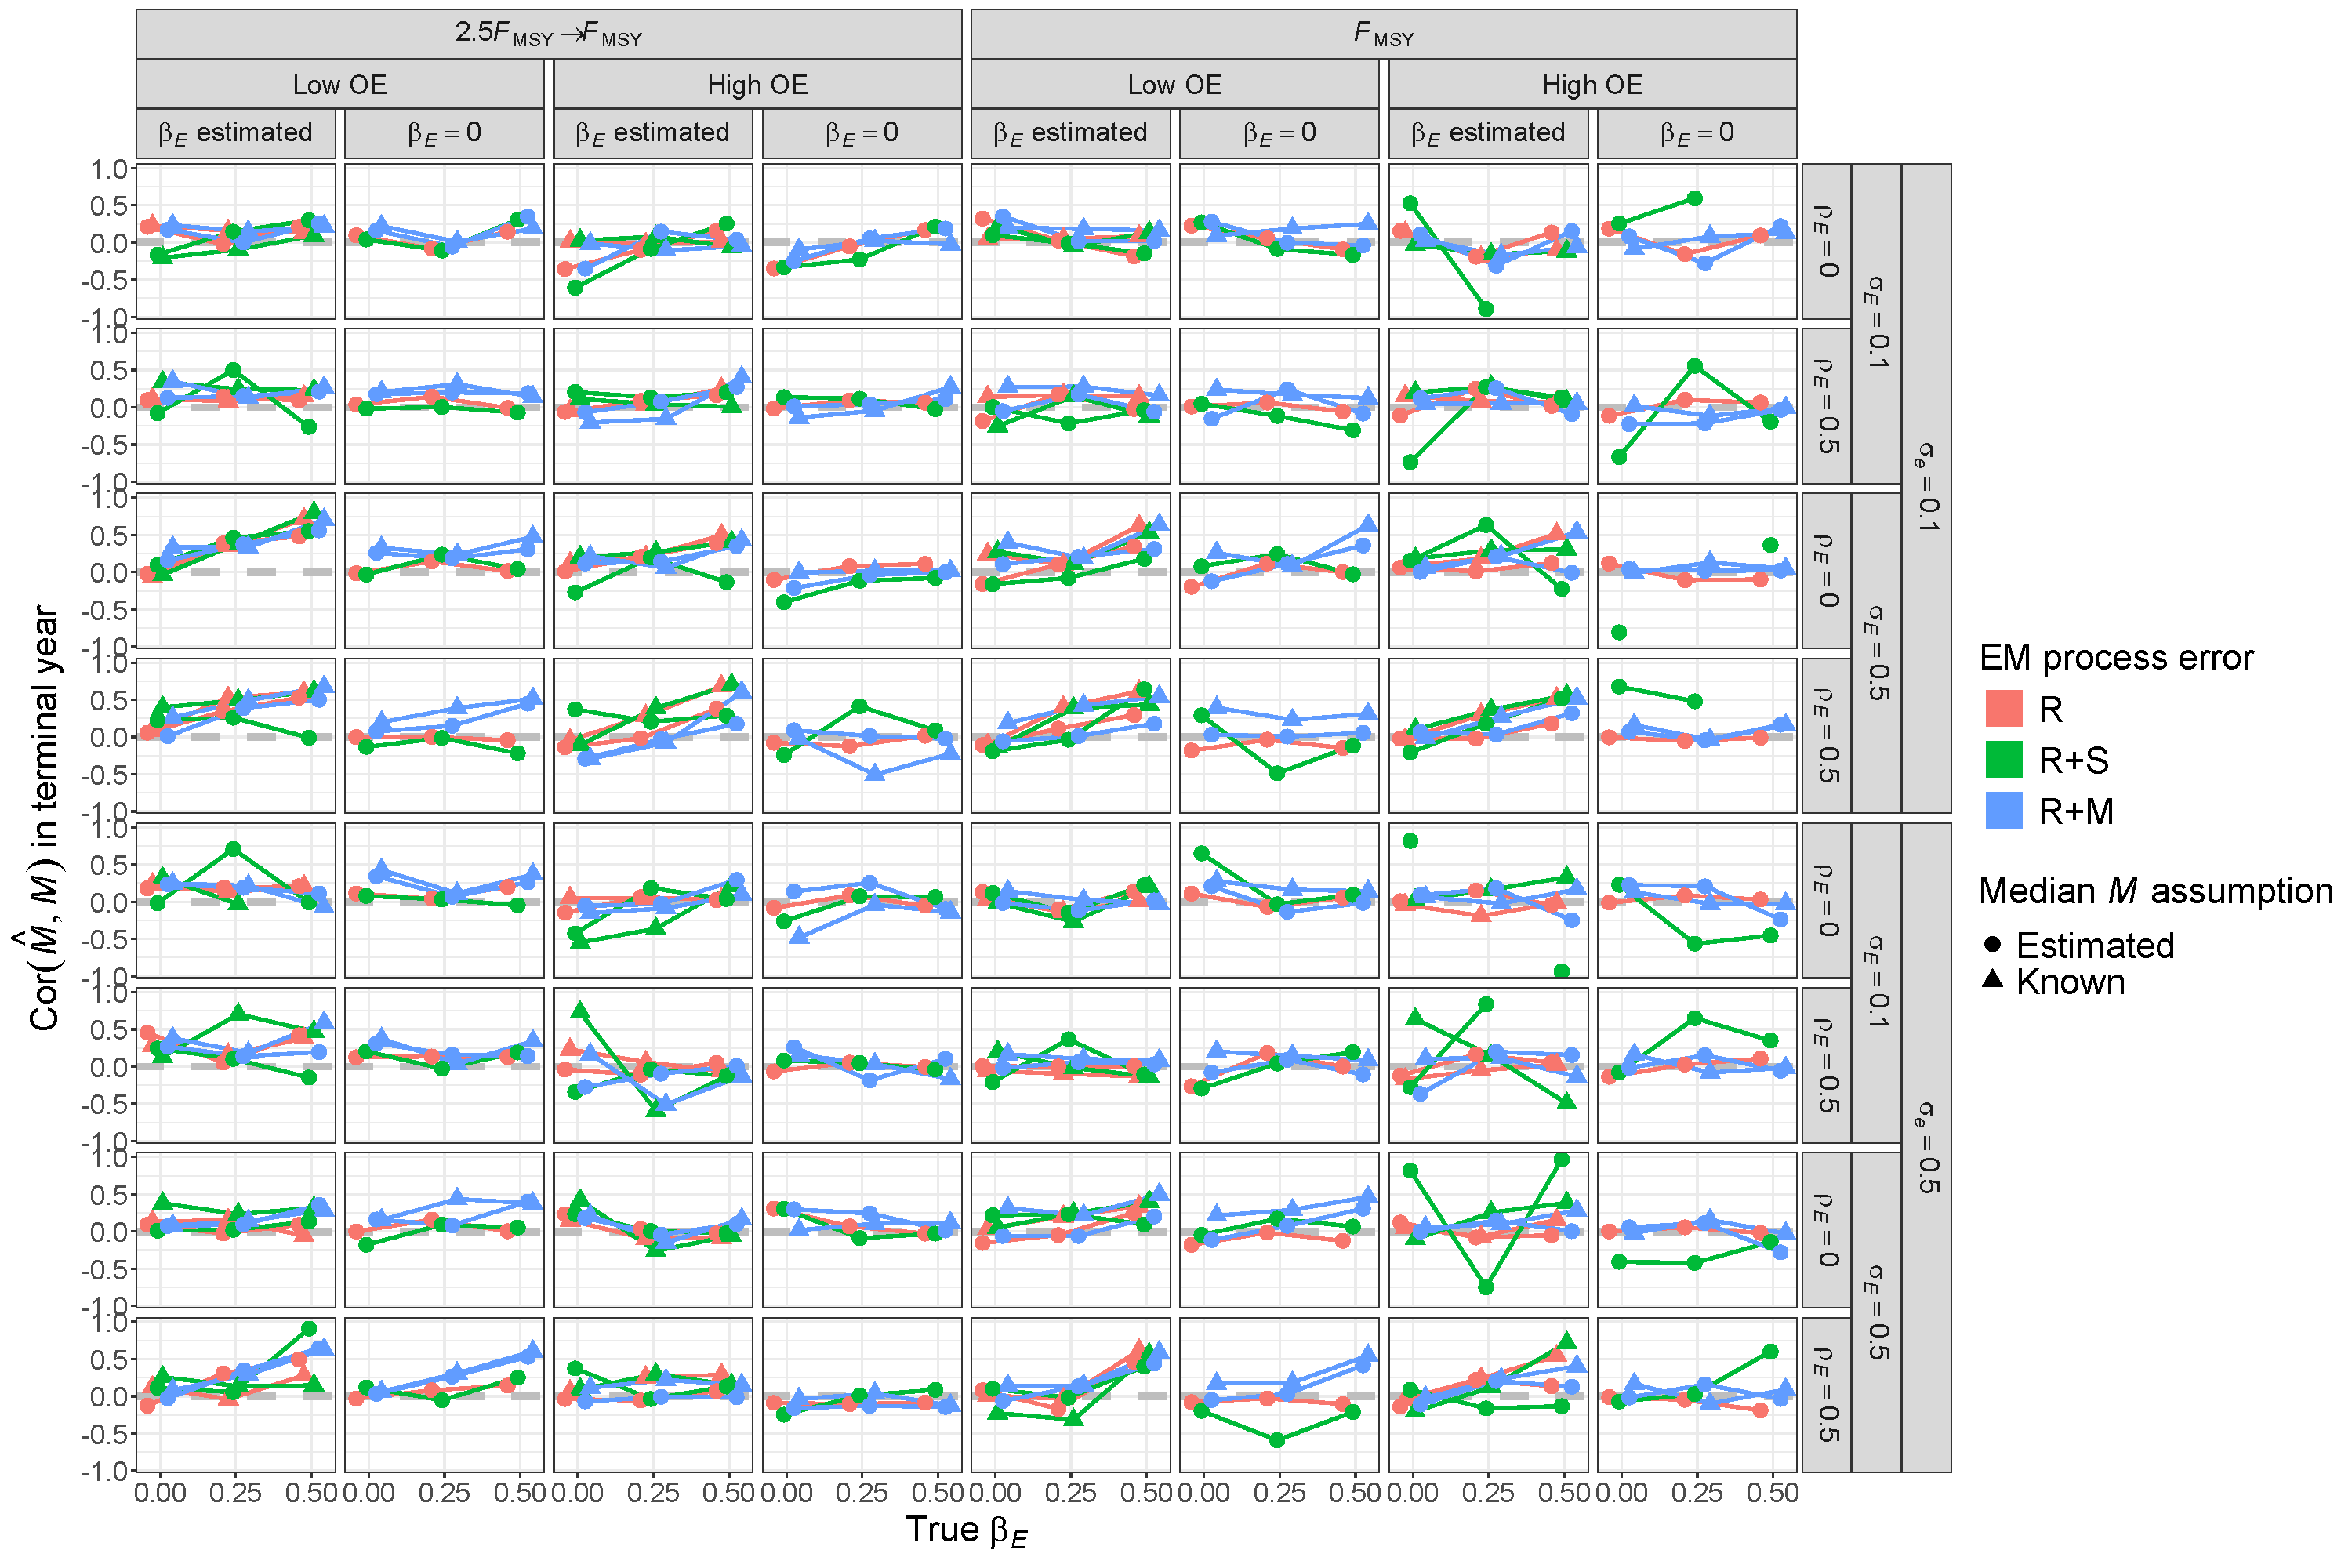
\includegraphics[height = \textheight]{terminal_year_M_corr_RMom}
%DIFDELCMD < \end{center}
%DIFDELCMD < %%%
%DIFDELCMD < \caption{%
{%DIFAUXCMD
\DIFdelFL{For R+M OMs, correlation of estimates and true vales of terminal year $M$ for EMs with alternative process error assumptions, treatment of covariate effect ($\beta_E = 0$ or estimated), and treatment of median $M$ parameter ($\beta_M$ estimated or known).}}%DIFAUXCMD
%DIFDELCMD < \label{terminal_M_corr_RMom}
%DIFDELCMD < \end{figure}
%DIFDELCMD < \end{landscape}
%DIFDELCMD < 

%DIFDELCMD < %%%
\subsection*{\DIFdel{Terminal year spawning stock biomass bias}}%DIFAUXCMD
%DIFDELCMD < \label{terminal-year-spawning-stock-biomass-bias}
%DIFDELCMD < %%%
\addcontentsline{toc}{subsection}{\DIFdel{Terminal year spawning stock biomass bias}}
%DIFAUXCMD
%DIFDELCMD < 

%DIFDELCMD < \begin{landscape}
%DIFDELCMD < \begin{figure}
%DIFDELCMD < \begin{center}
%DIFDELCMD < 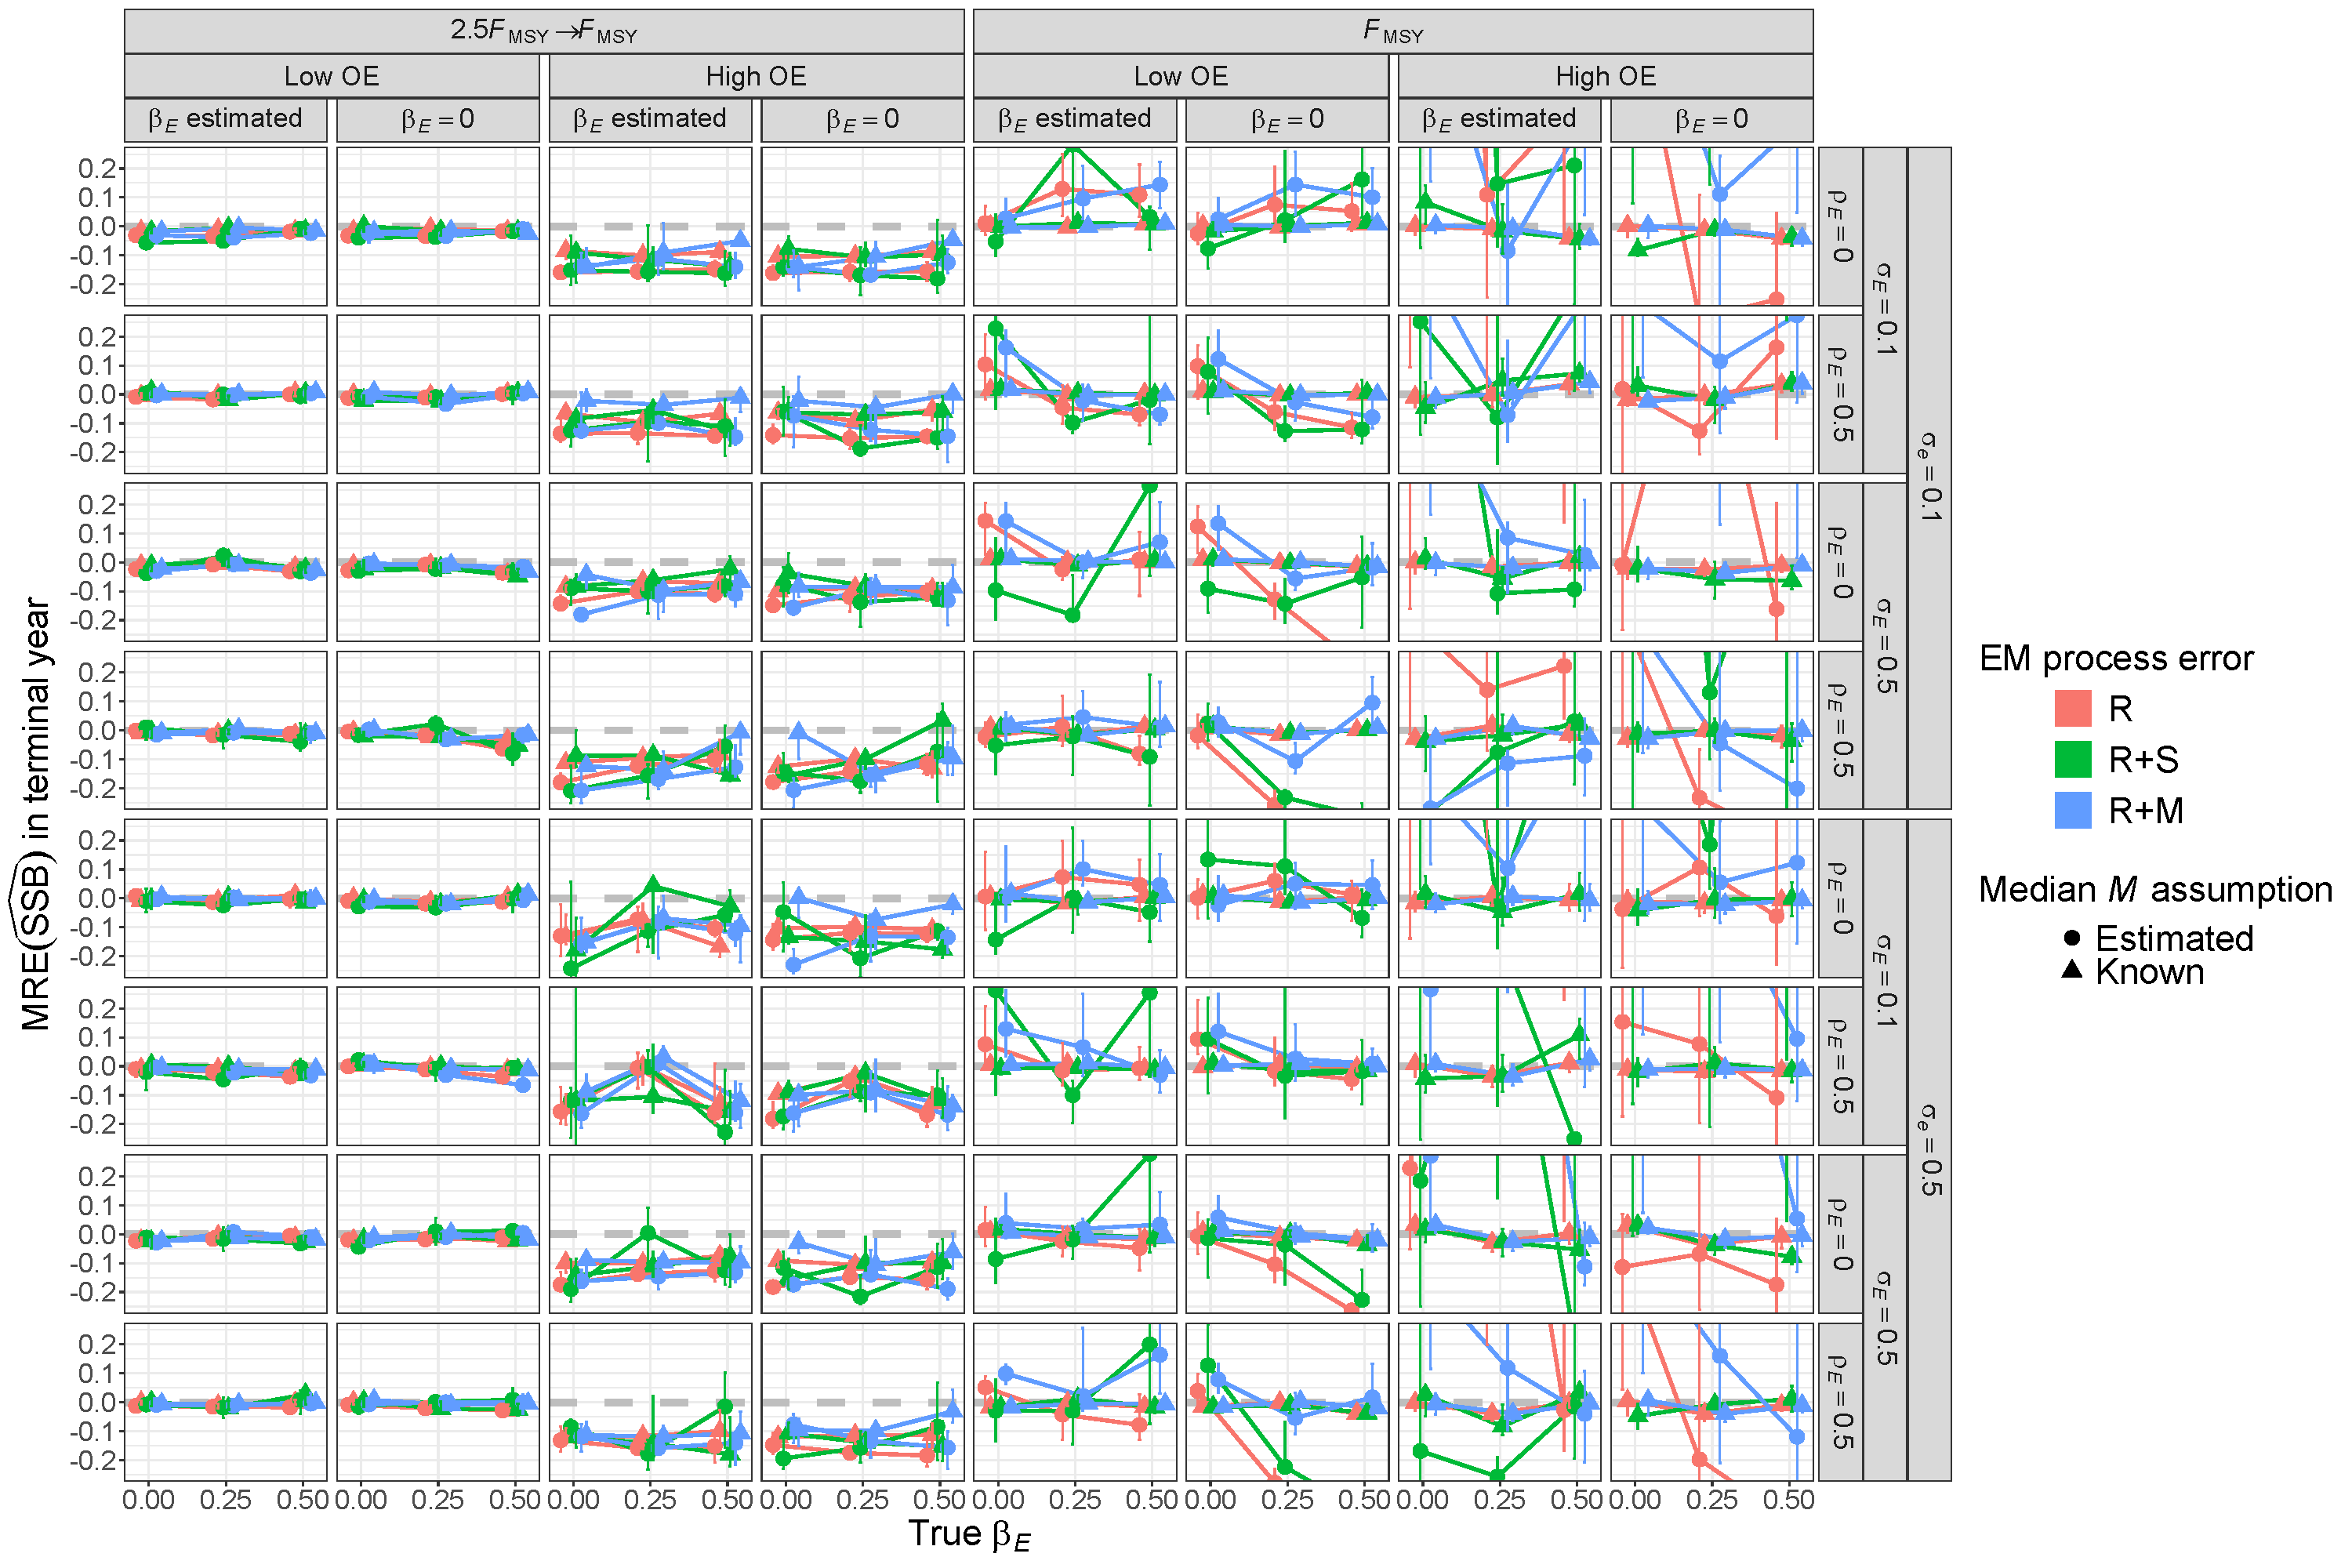
\includegraphics[height = \textheight]{terminal_year_ssb_bias_Rom}
%DIFDELCMD < \end{center}
%DIFDELCMD < %%%
%DIFDELCMD < \caption{%
{%DIFAUXCMD
\DIFdelFL{For R OMs, median relative error (MRE) of estimates of SSB in the terminal year for EMs with alternative process error assumptions, treatment of covariate effect ($\beta_E = 0$ or estimated), and treatment of median $M$ parameter ($\beta_M$ estimated or known).}}%DIFAUXCMD
%DIFDELCMD < \label{terminal_ssb_bias_Rom}
%DIFDELCMD < \end{figure}
%DIFDELCMD < \end{landscape}
%DIFDELCMD < 

%DIFDELCMD < \begin{landscape}
%DIFDELCMD < \begin{figure}
%DIFDELCMD < \begin{center}
%DIFDELCMD < 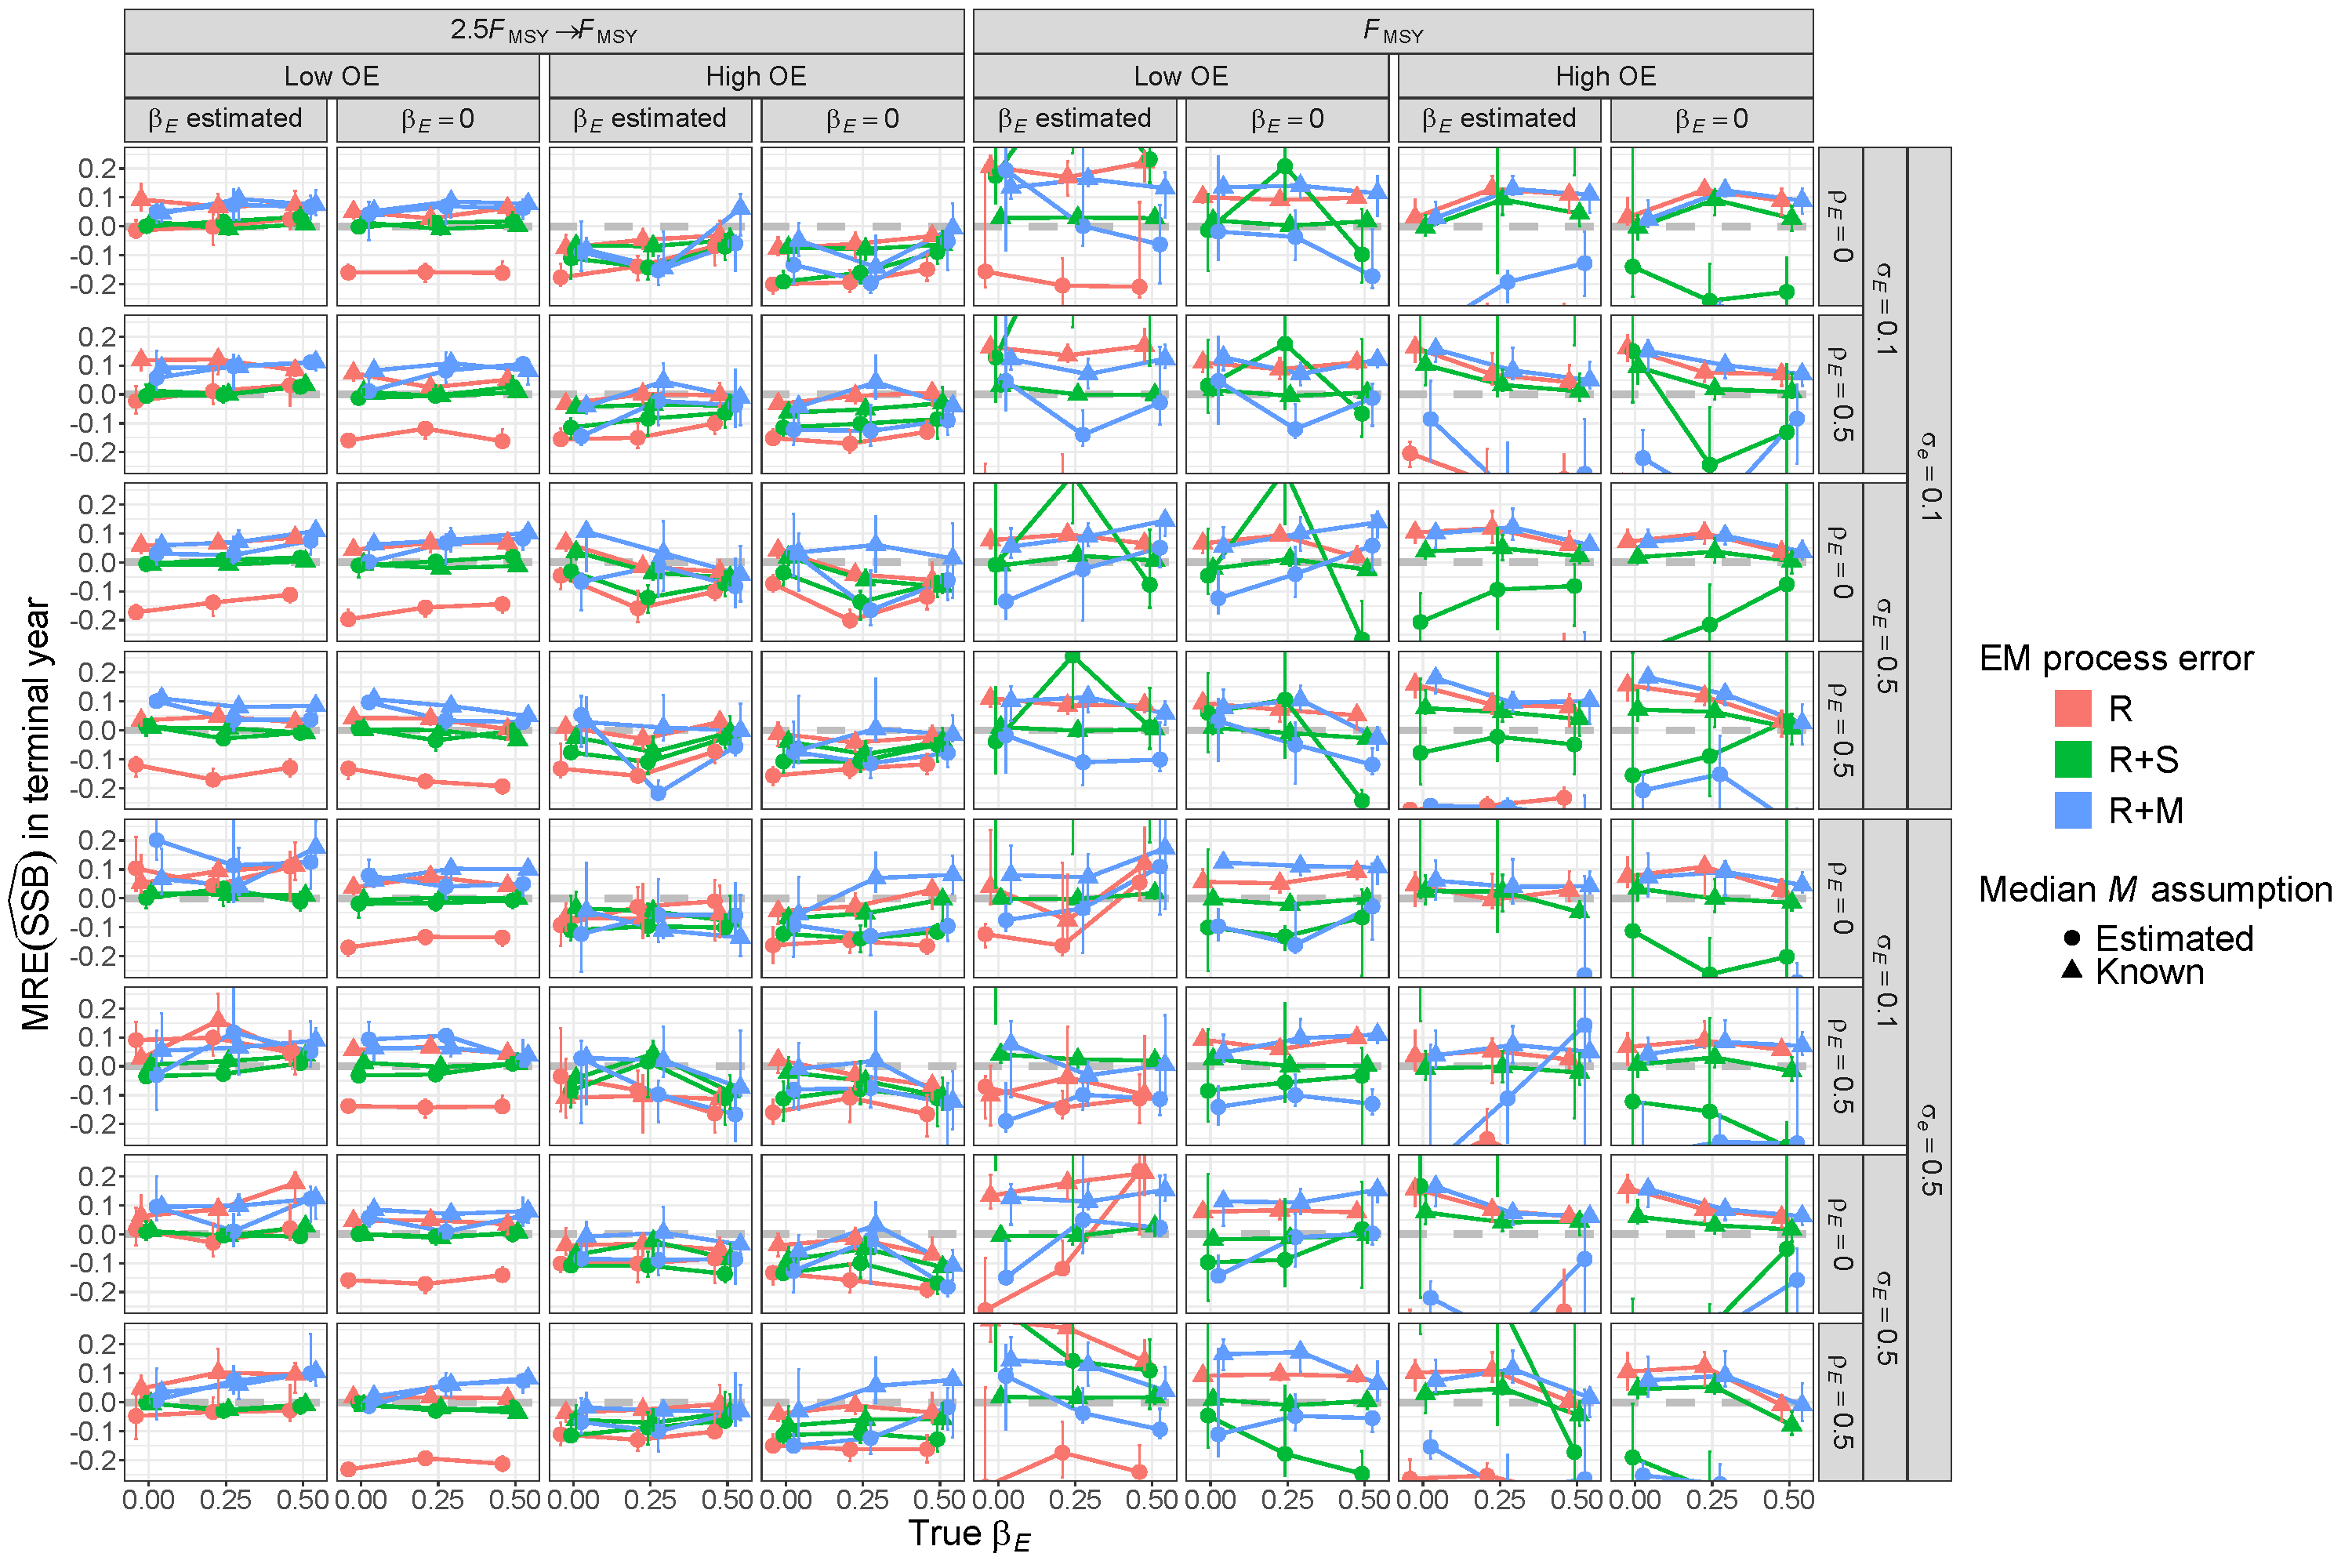
\includegraphics[height = \textheight]{terminal_year_ssb_bias_RSom}
%DIFDELCMD < \end{center}
%DIFDELCMD < %%%
%DIFDELCMD < \caption{%
{%DIFAUXCMD
\DIFdelFL{For R+S OMs, median relative error (MRE) of SSB in the terminal year for EMs with alternative process error assumptions, treatment of covariate effect ($\beta_E = 0$ or estimated), and treatment of median $M$ parameter ($\beta_M$ estimated or known).}}%DIFAUXCMD
%DIFDELCMD < \label{terminal_ssb_bias_RSom}
%DIFDELCMD < \end{figure}
%DIFDELCMD < \end{landscape}
%DIFDELCMD < 

%DIFDELCMD < \begin{landscape}
%DIFDELCMD < \begin{figure}
%DIFDELCMD < \begin{center}
%DIFDELCMD < 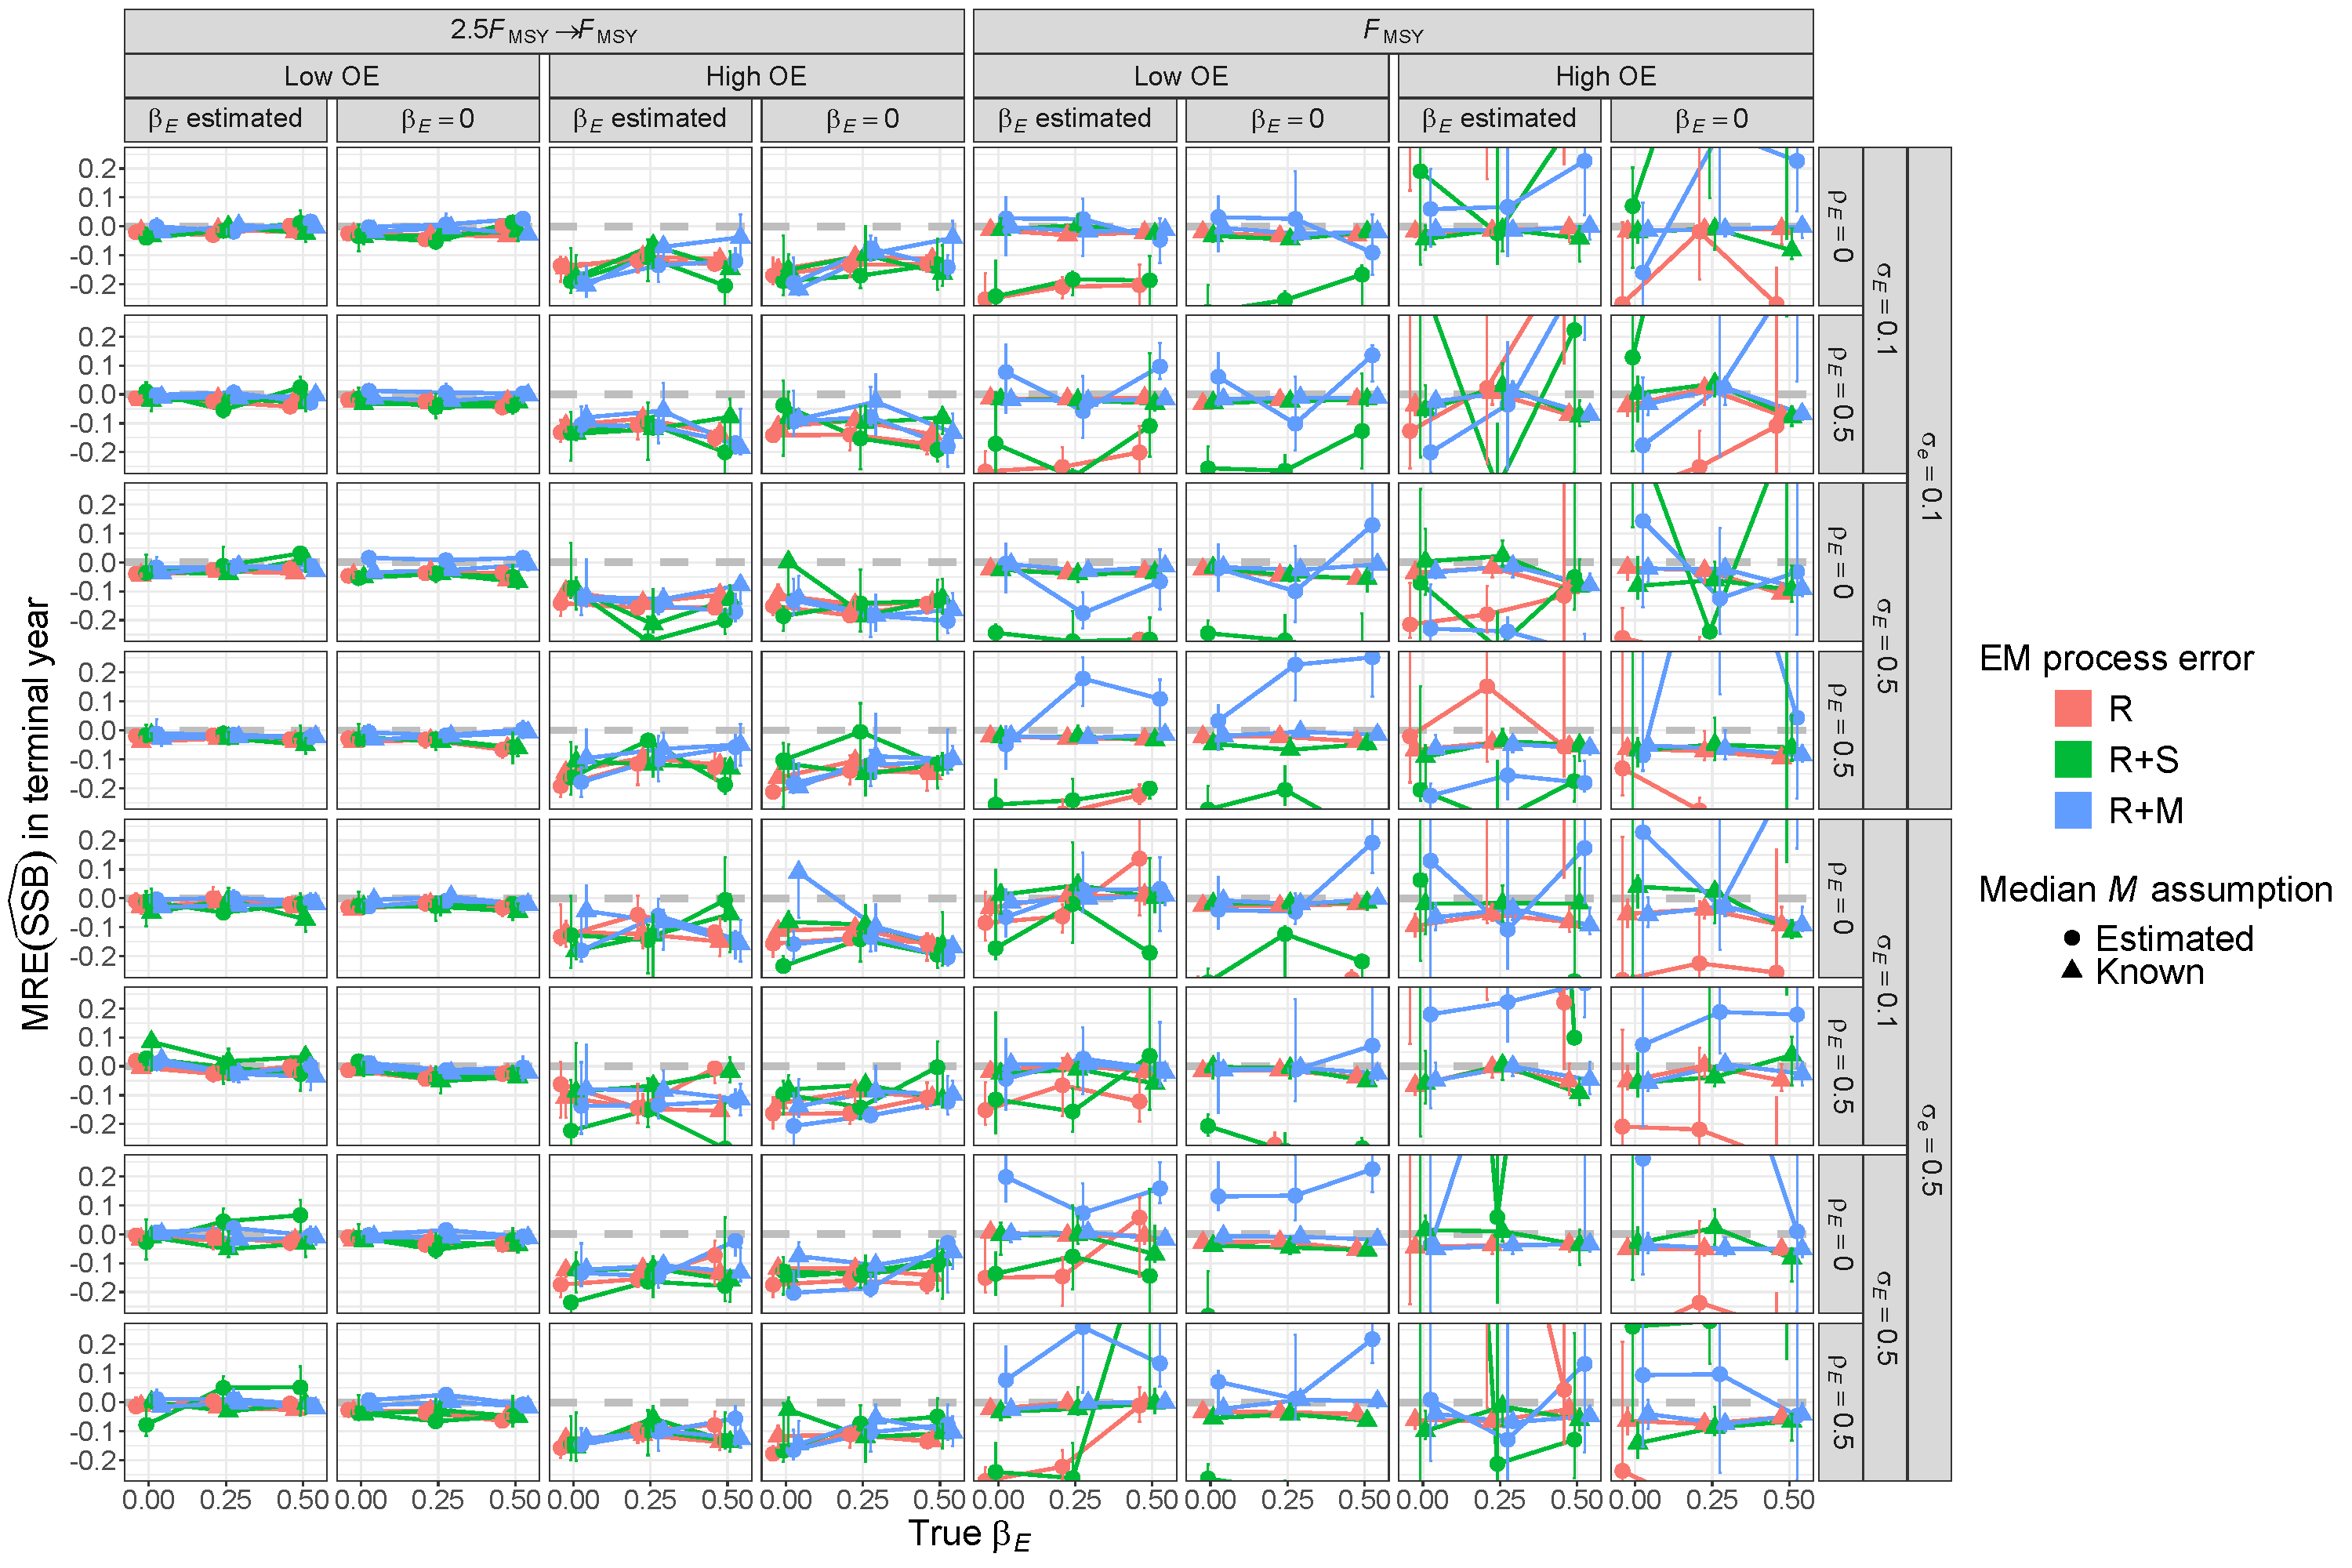
\includegraphics[height = \textheight]{terminal_year_ssb_bias_RMom}
%DIFDELCMD < \end{center}
%DIFDELCMD < %%%
%DIFDELCMD < \caption{%
{%DIFAUXCMD
\DIFdelFL{For R+M OMs, median relative error (MRE) of estimates of SSB in the terminal year for EMs with alternative process error assumptions, treatment of covariate effect ($\beta_E = 0$ or estimated), and treatment of median $M$ parameter ($\beta_M$ estimated or known).}}%DIFAUXCMD
%DIFDELCMD < \label{terminal_ssb_bias_RMom}
%DIFDELCMD < \end{figure}
%DIFDELCMD < \end{landscape}
%DIFDELCMD < 

%DIFDELCMD < %%%
\subsection*{\DIFdel{Terminal year spawning stock biomass accuracy}}%DIFAUXCMD
%DIFDELCMD < \label{terminal-year-spawning-stock-biomass-accuracy}
%DIFDELCMD < %%%
\addcontentsline{toc}{subsection}{\DIFdel{Terminal year spawning stock biomass accuracy}}
%DIFAUXCMD
%DIFDELCMD < 

%DIFDELCMD < \begin{landscape}
%DIFDELCMD < \begin{figure}
%DIFDELCMD < \begin{center}
%DIFDELCMD < %%%
\DIFdelendFL 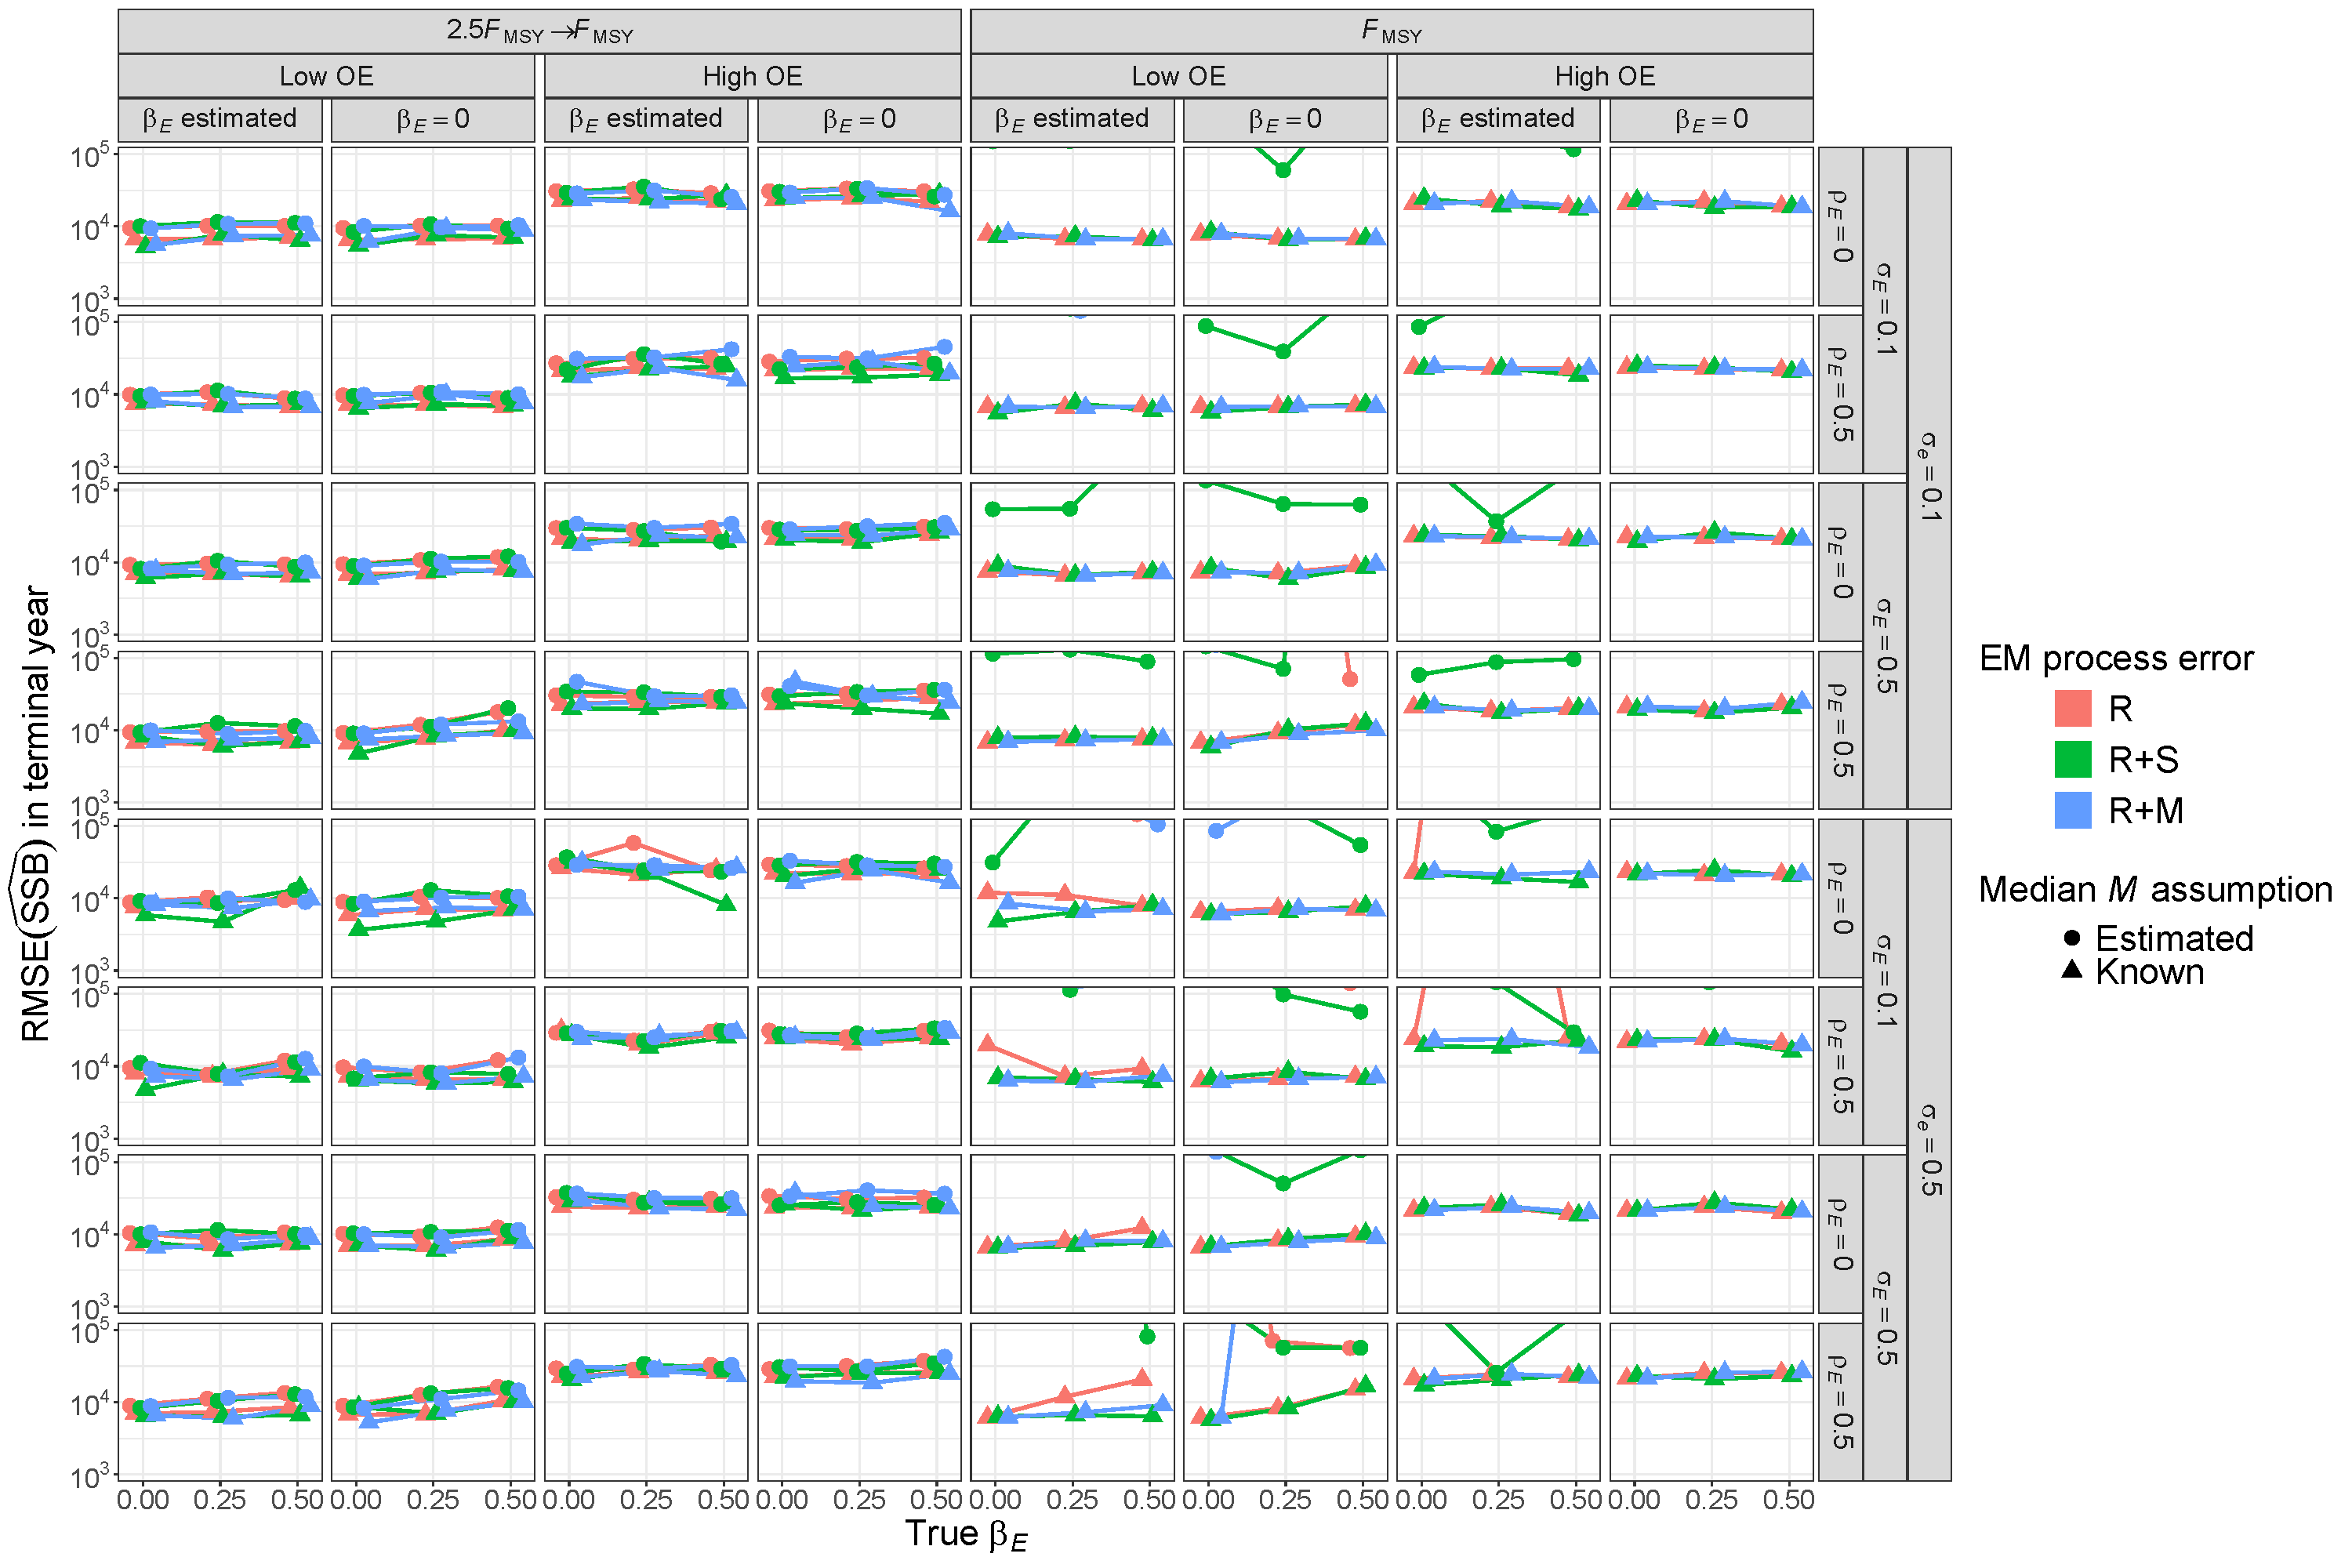
\includegraphics[height = \textheight]{terminal_year_ssb_rmse_Rom}
\end{center}
\caption{For R \DIFdelbeginFL \DIFdelFL{OMs}\DIFdelendFL \DIFaddbeginFL \DIFaddFL{operating models}\DIFaddendFL , RMSE of estimates of SSB in the terminal year for \DIFdelbeginFL \DIFdelFL{EMs }\DIFdelendFL \DIFaddbeginFL \DIFaddFL{estimating models }\DIFaddendFL with alternative process error assumptions, treatment of covariate effect ($\beta_E = 0$ or estimated), and treatment of median $M$ parameter ($\beta_M$ estimated or known).}\label{terminal_ssb_rmse_Rom}
\end{figure}
\end{landscape}

\begin{landscape}
\begin{figure}
\begin{center}
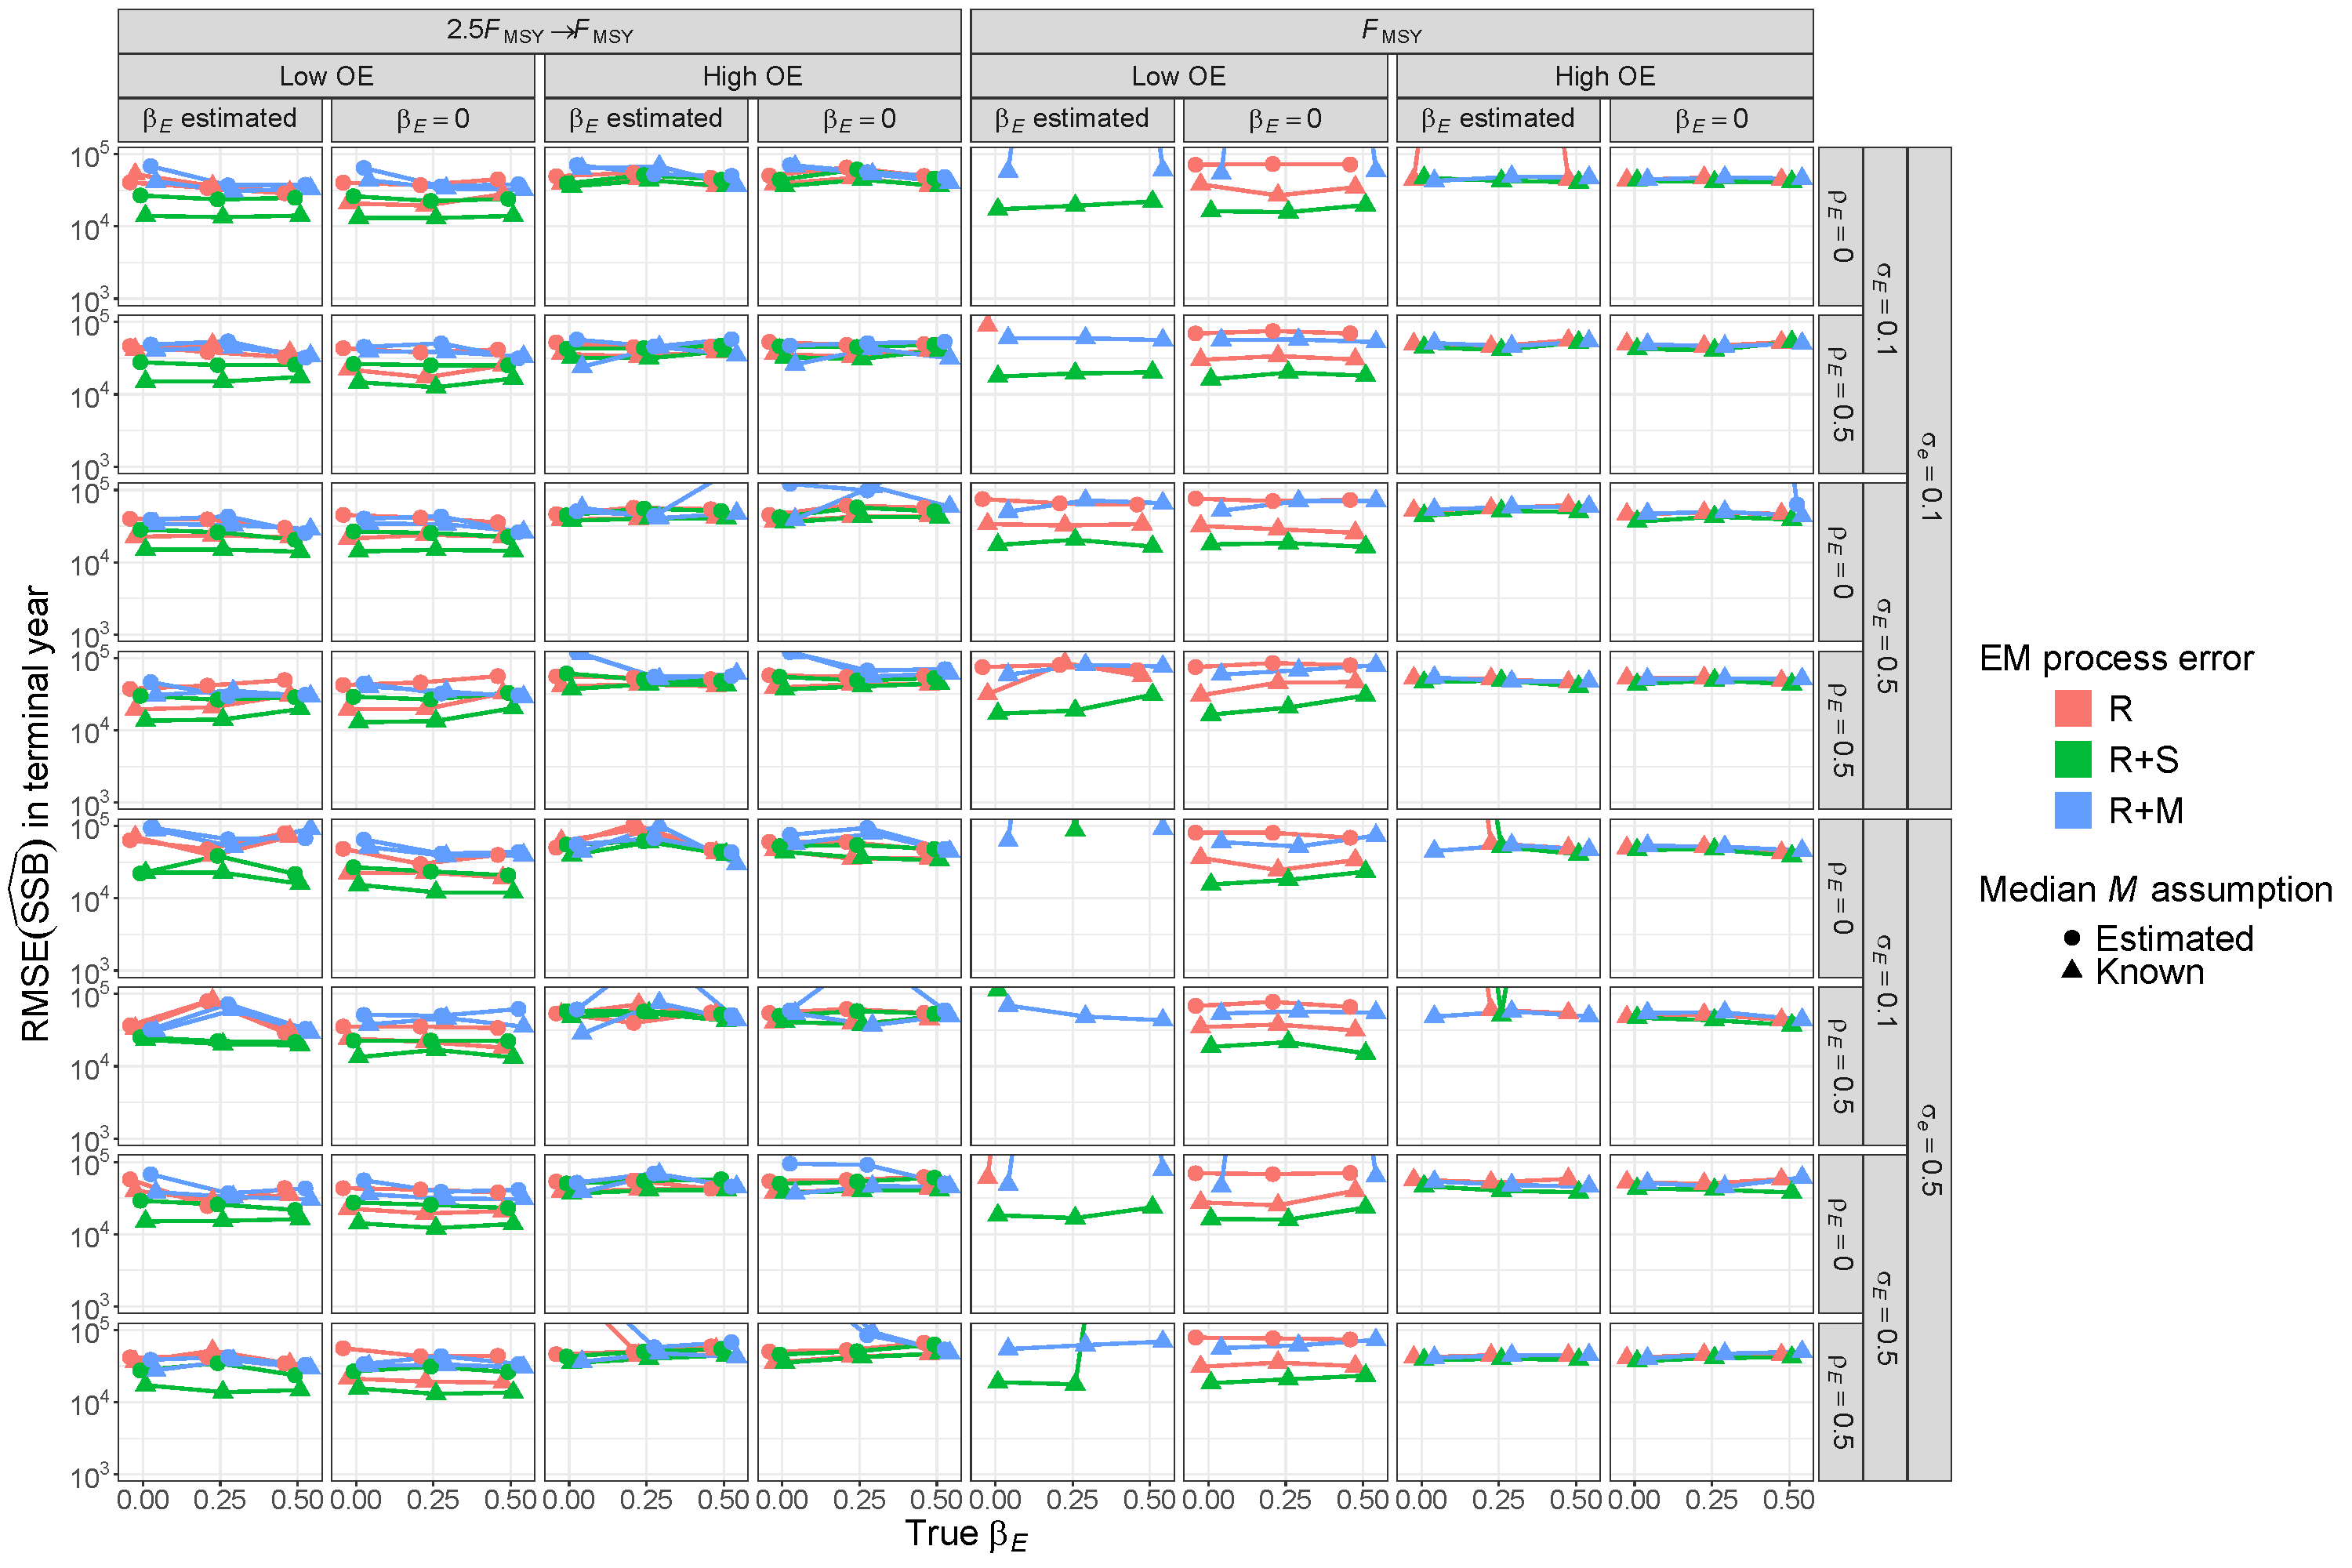
\includegraphics[height = \textheight]{terminal_year_ssb_rmse_RSom}
\end{center}
\caption{For R+S \DIFdelbeginFL \DIFdelFL{OMs}\DIFdelendFL \DIFaddbeginFL \DIFaddFL{operating models}\DIFaddendFL , RMSE of estimates of SSB in the terminal year for \DIFdelbeginFL \DIFdelFL{EMs }\DIFdelendFL \DIFaddbeginFL \DIFaddFL{estimating models }\DIFaddendFL with alternative process error assumptions, treatment of covariate effect ($\beta_E = 0$ or estimated), and treatment of median $M$ parameter ($\beta_M$ estimated or known).}\label{terminal_ssb_rmse_RSom}
\end{figure}
\end{landscape}

\begin{landscape}
\begin{figure}
\begin{center}
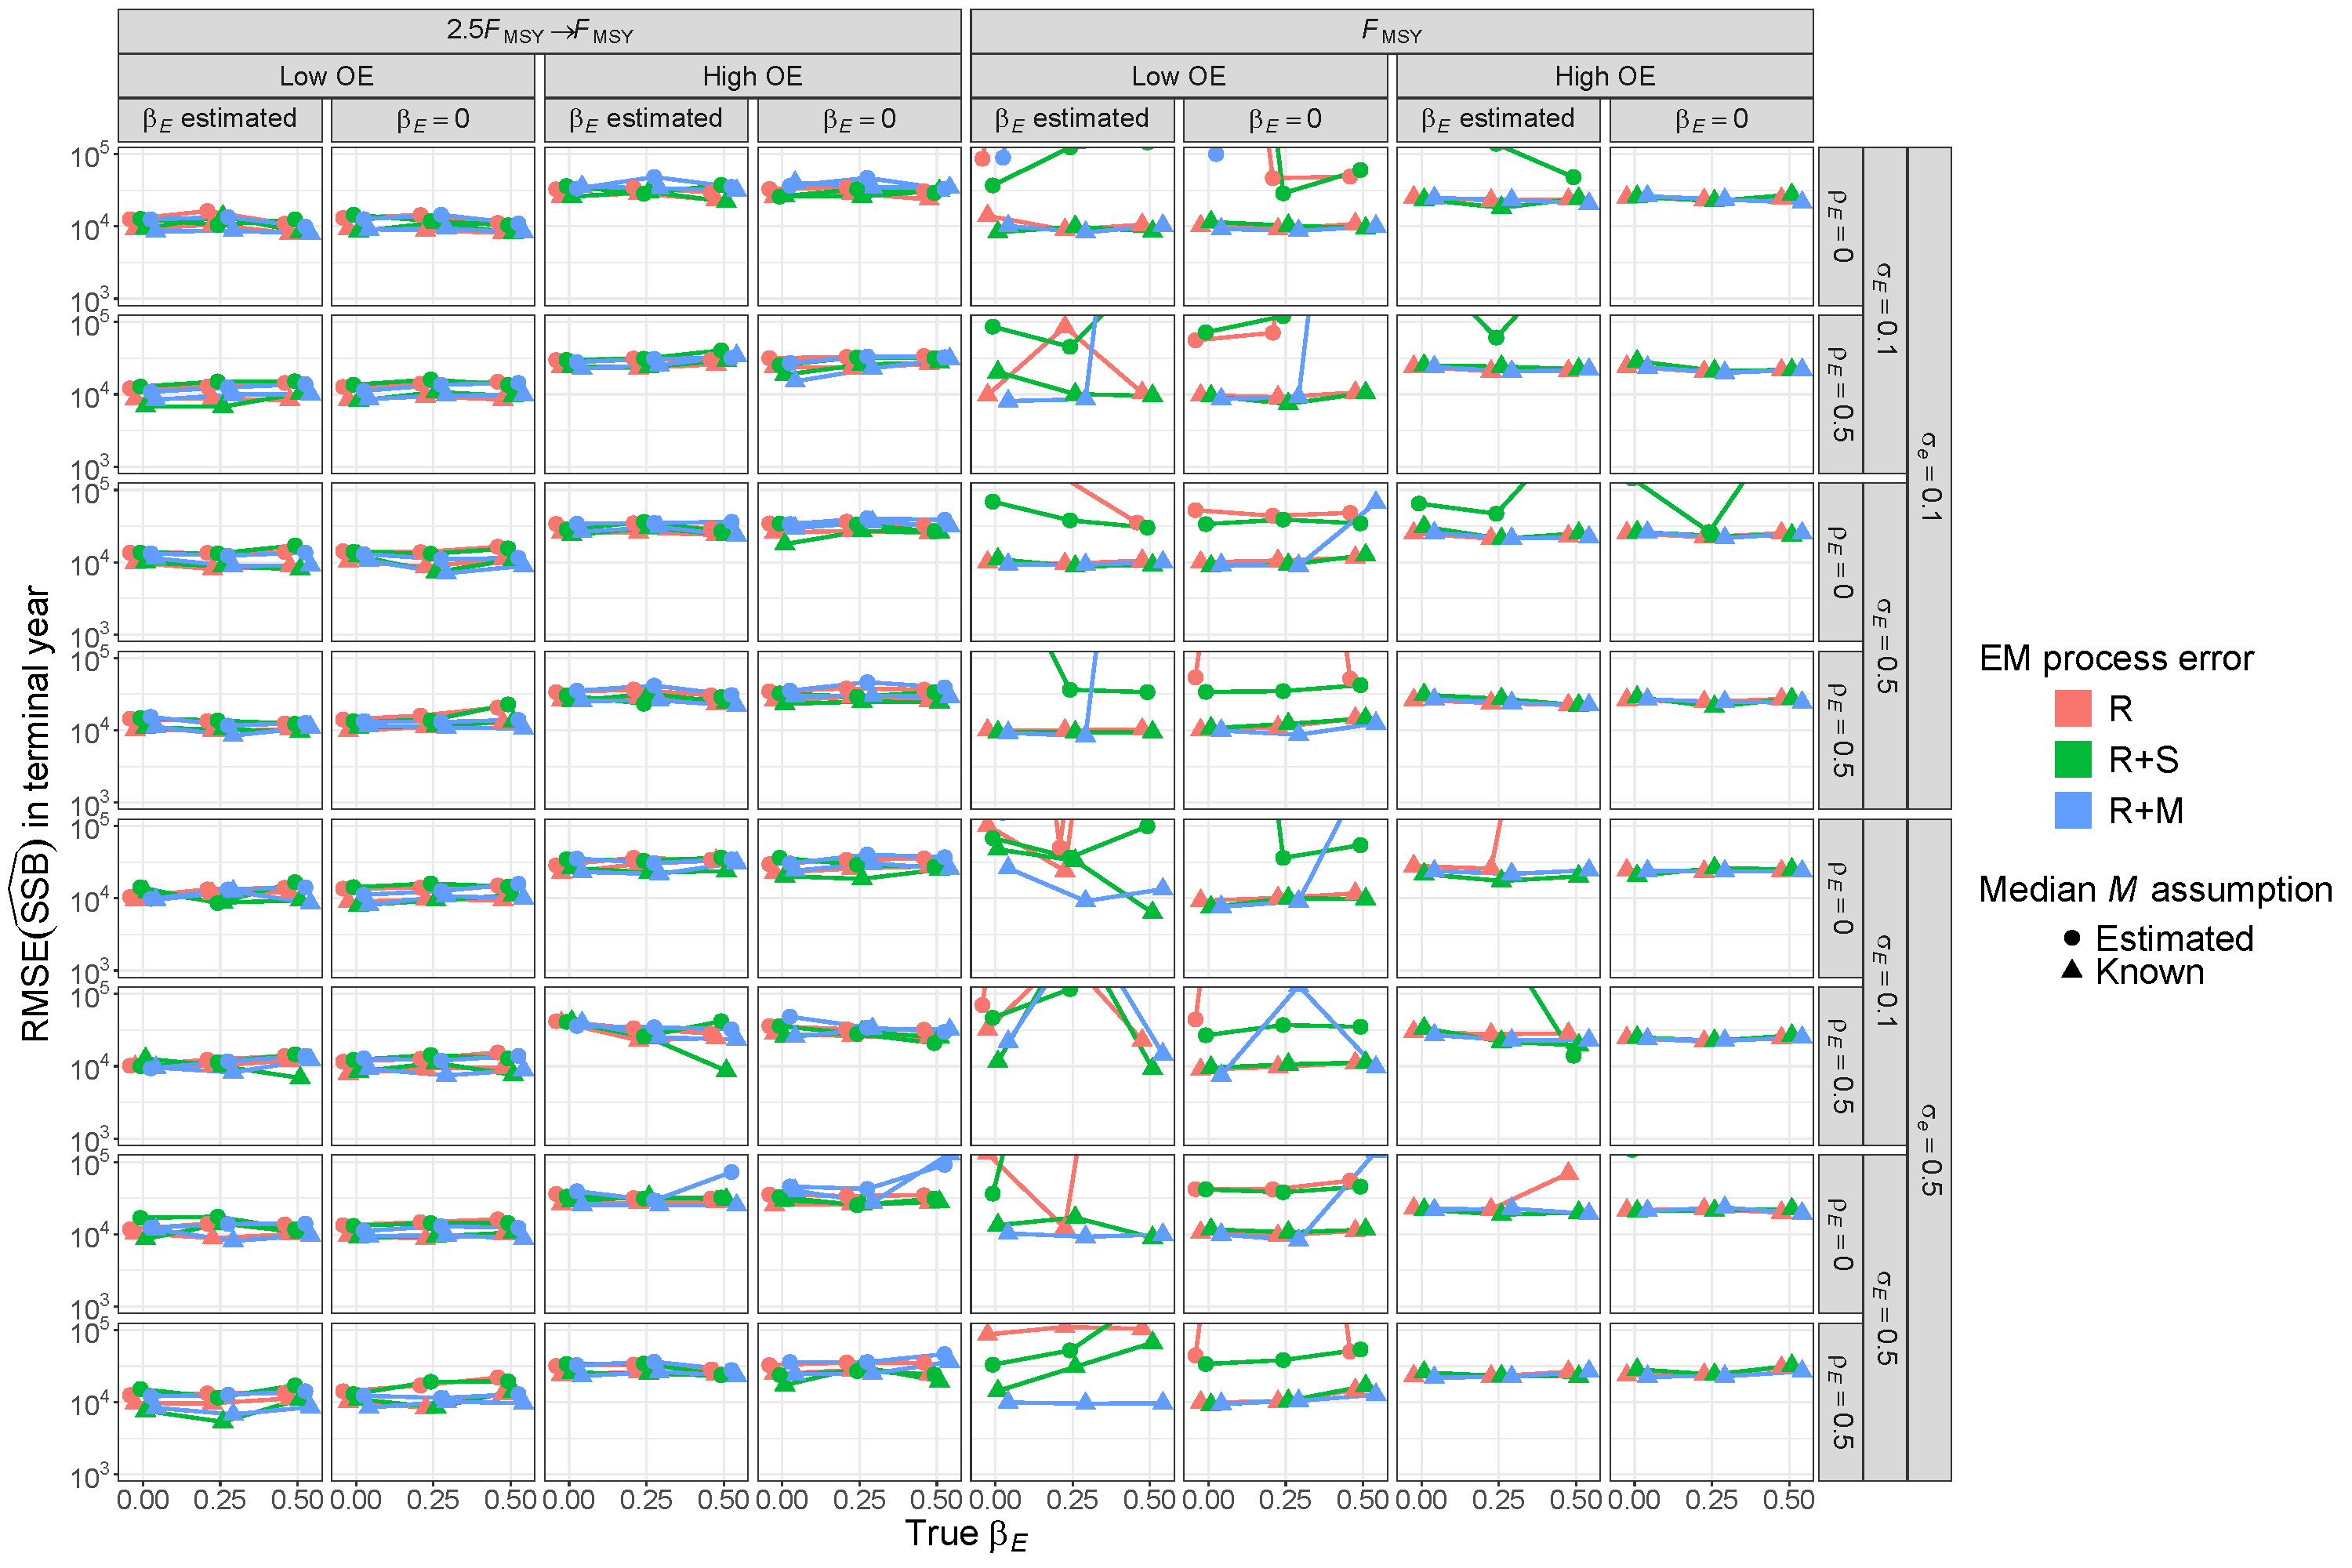
\includegraphics[height = \textheight]{terminal_year_ssb_rmse_RMom}
\end{center}
\caption{For R+M \DIFdelbeginFL \DIFdelFL{OMs}\DIFdelendFL \DIFaddbeginFL \DIFaddFL{operating models}\DIFaddendFL , RMSE of estimates of SSB in the terminal year for \DIFdelbeginFL \DIFdelFL{EMs }\DIFdelendFL \DIFaddbeginFL \DIFaddFL{estimating models }\DIFaddendFL with alternative process error assumptions, treatment of covariate effect ($\beta_E = 0$ or estimated), and treatment of median $M$ parameter ($\beta_M$ estimated or known).}\label{terminal_ssb_rmse_RMom}
\end{figure}
\end{landscape}

\begin{landscape}
\begin{figure}
\begin{center}
\DIFdelbeginFL %DIFDELCMD < 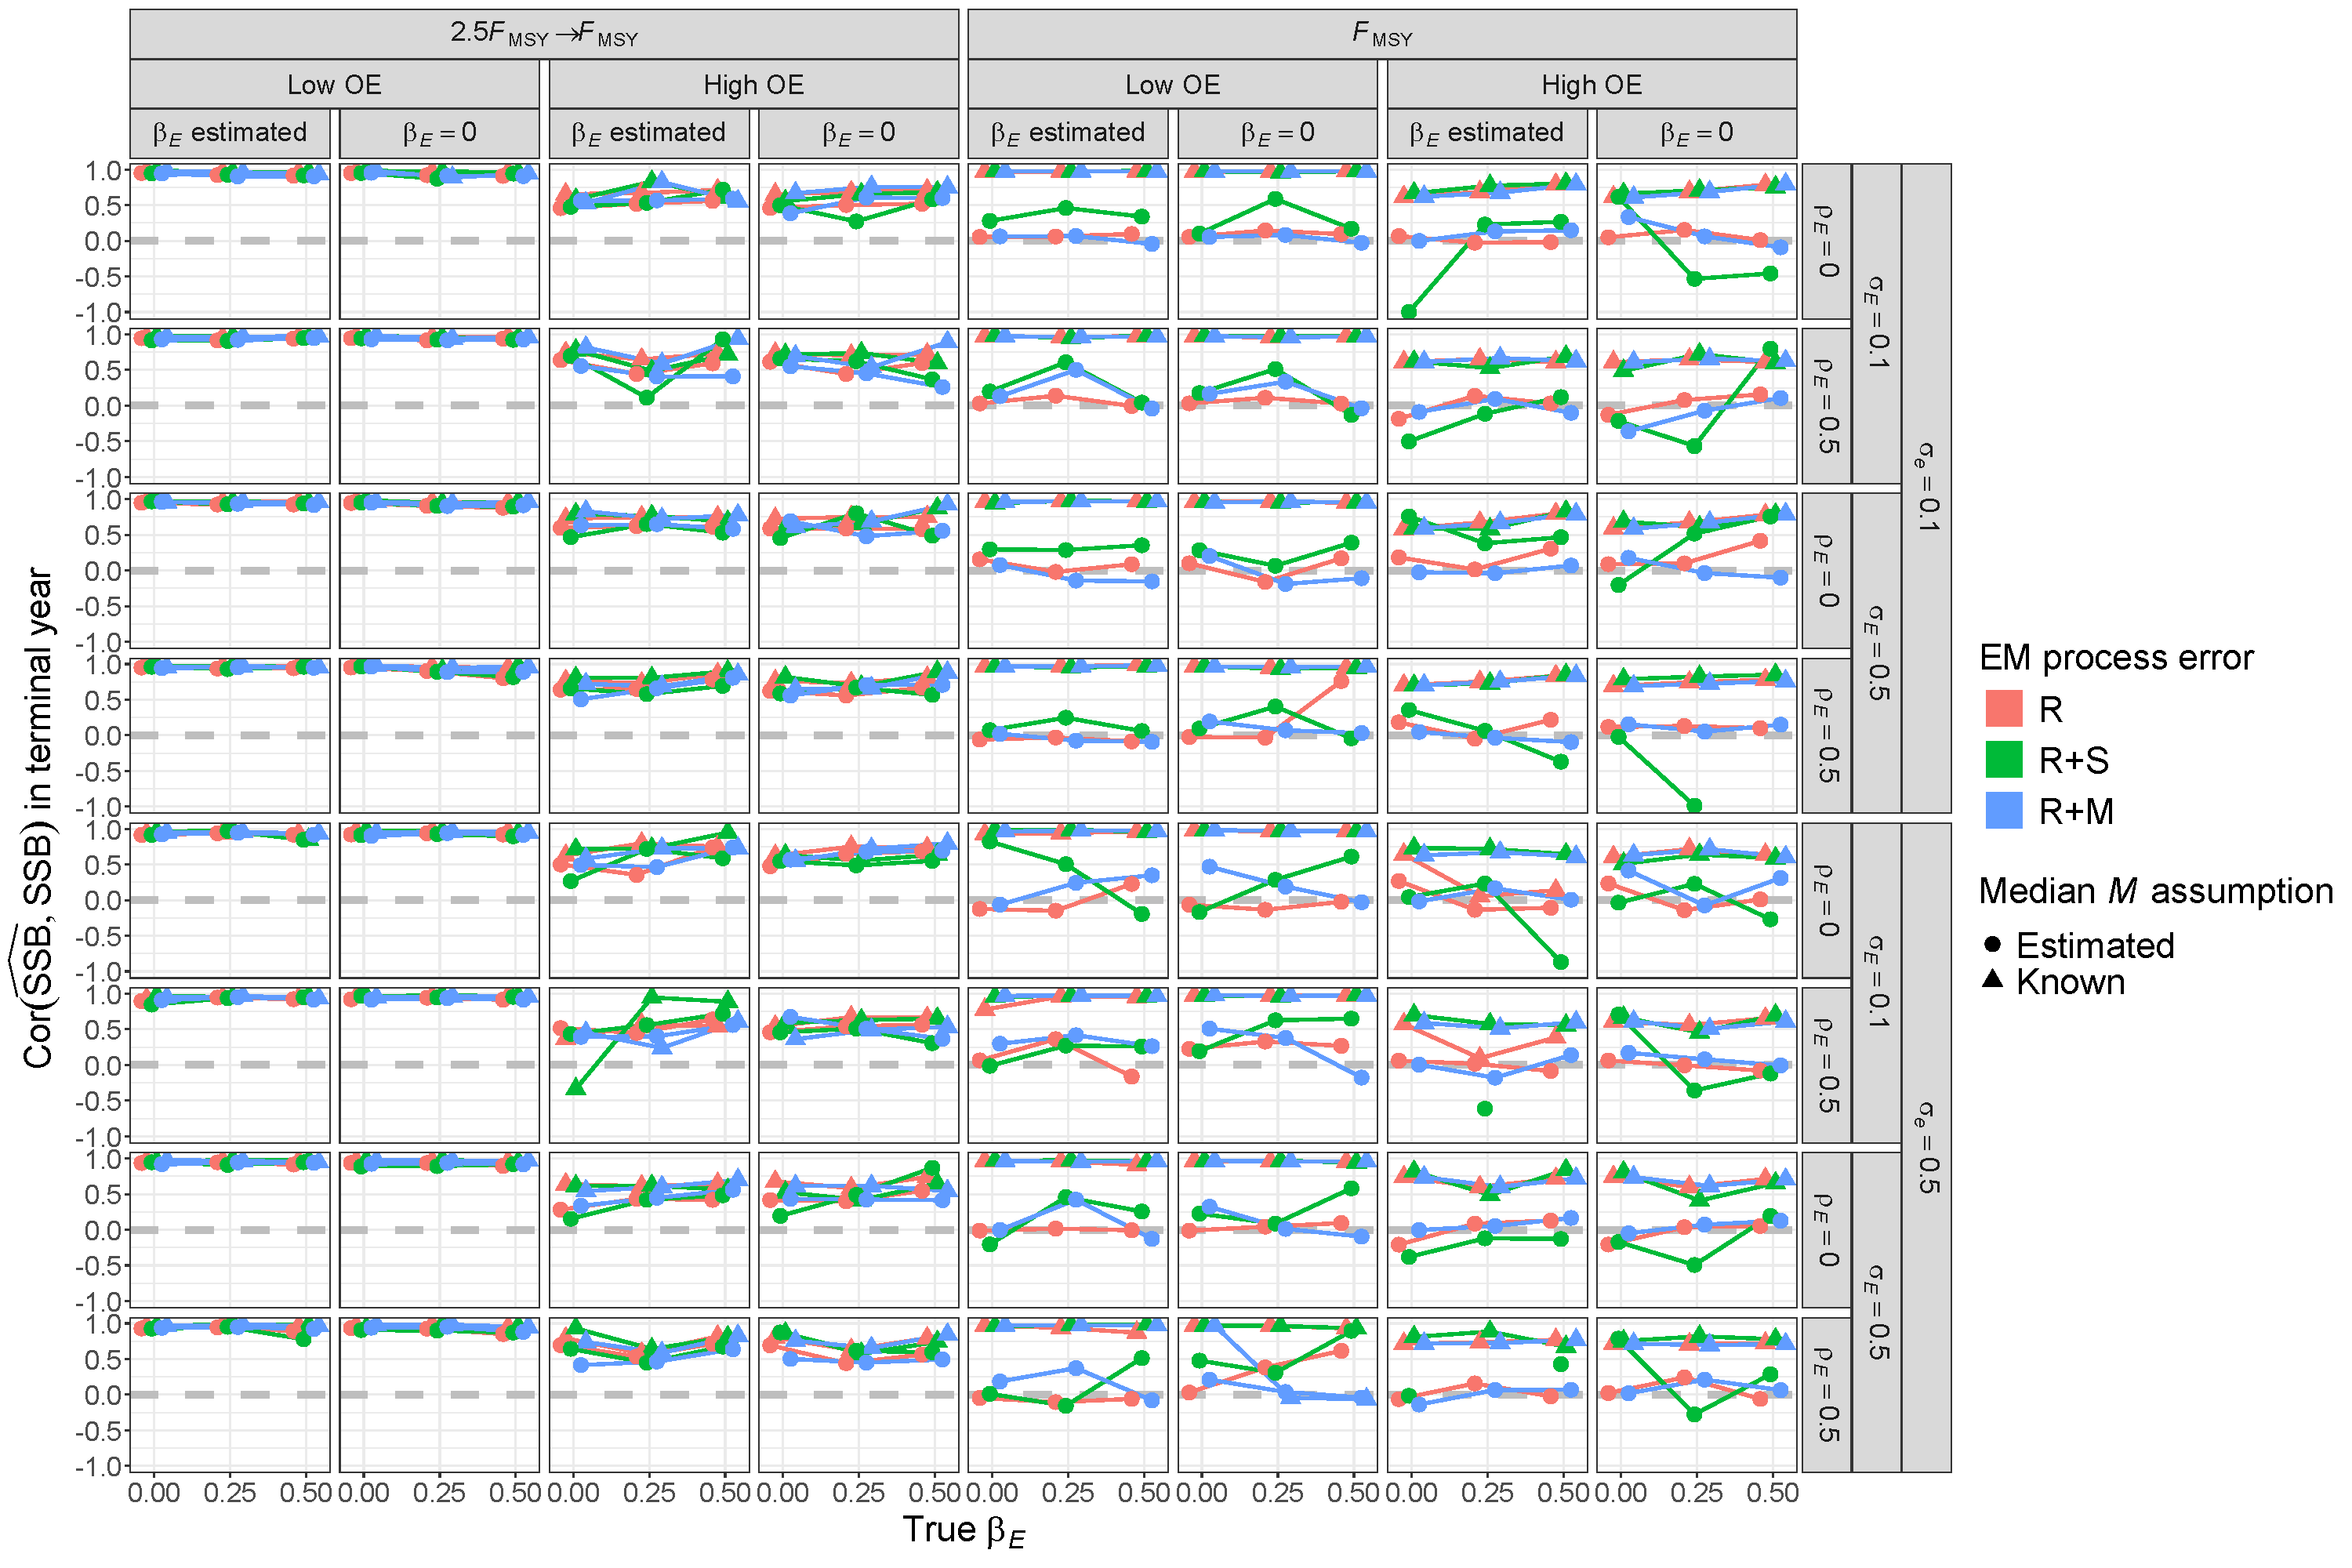
\includegraphics[height = \textheight]{terminal_year_ssb_corr_Rom}
%DIFDELCMD < \end{center}
%DIFDELCMD < %%%
%DIFDELCMD < \caption{%
{%DIFAUXCMD
\DIFdelFL{For R OMs, correlation of estimates and true values of terminal year SSB for EMs with alternative process error assumptions, treatment of covariate effect ($\beta_E = 0$ or estimated), and treatment of median $M$ parameter ($\beta_M$ estimated or known).}}%DIFAUXCMD
%DIFDELCMD < \label{terminal_ssb_corr_Rom}
%DIFDELCMD < \end{figure}
%DIFDELCMD < \end{landscape}
%DIFDELCMD < 

%DIFDELCMD < \begin{landscape}
%DIFDELCMD < \begin{figure}
%DIFDELCMD < \begin{center}
%DIFDELCMD < 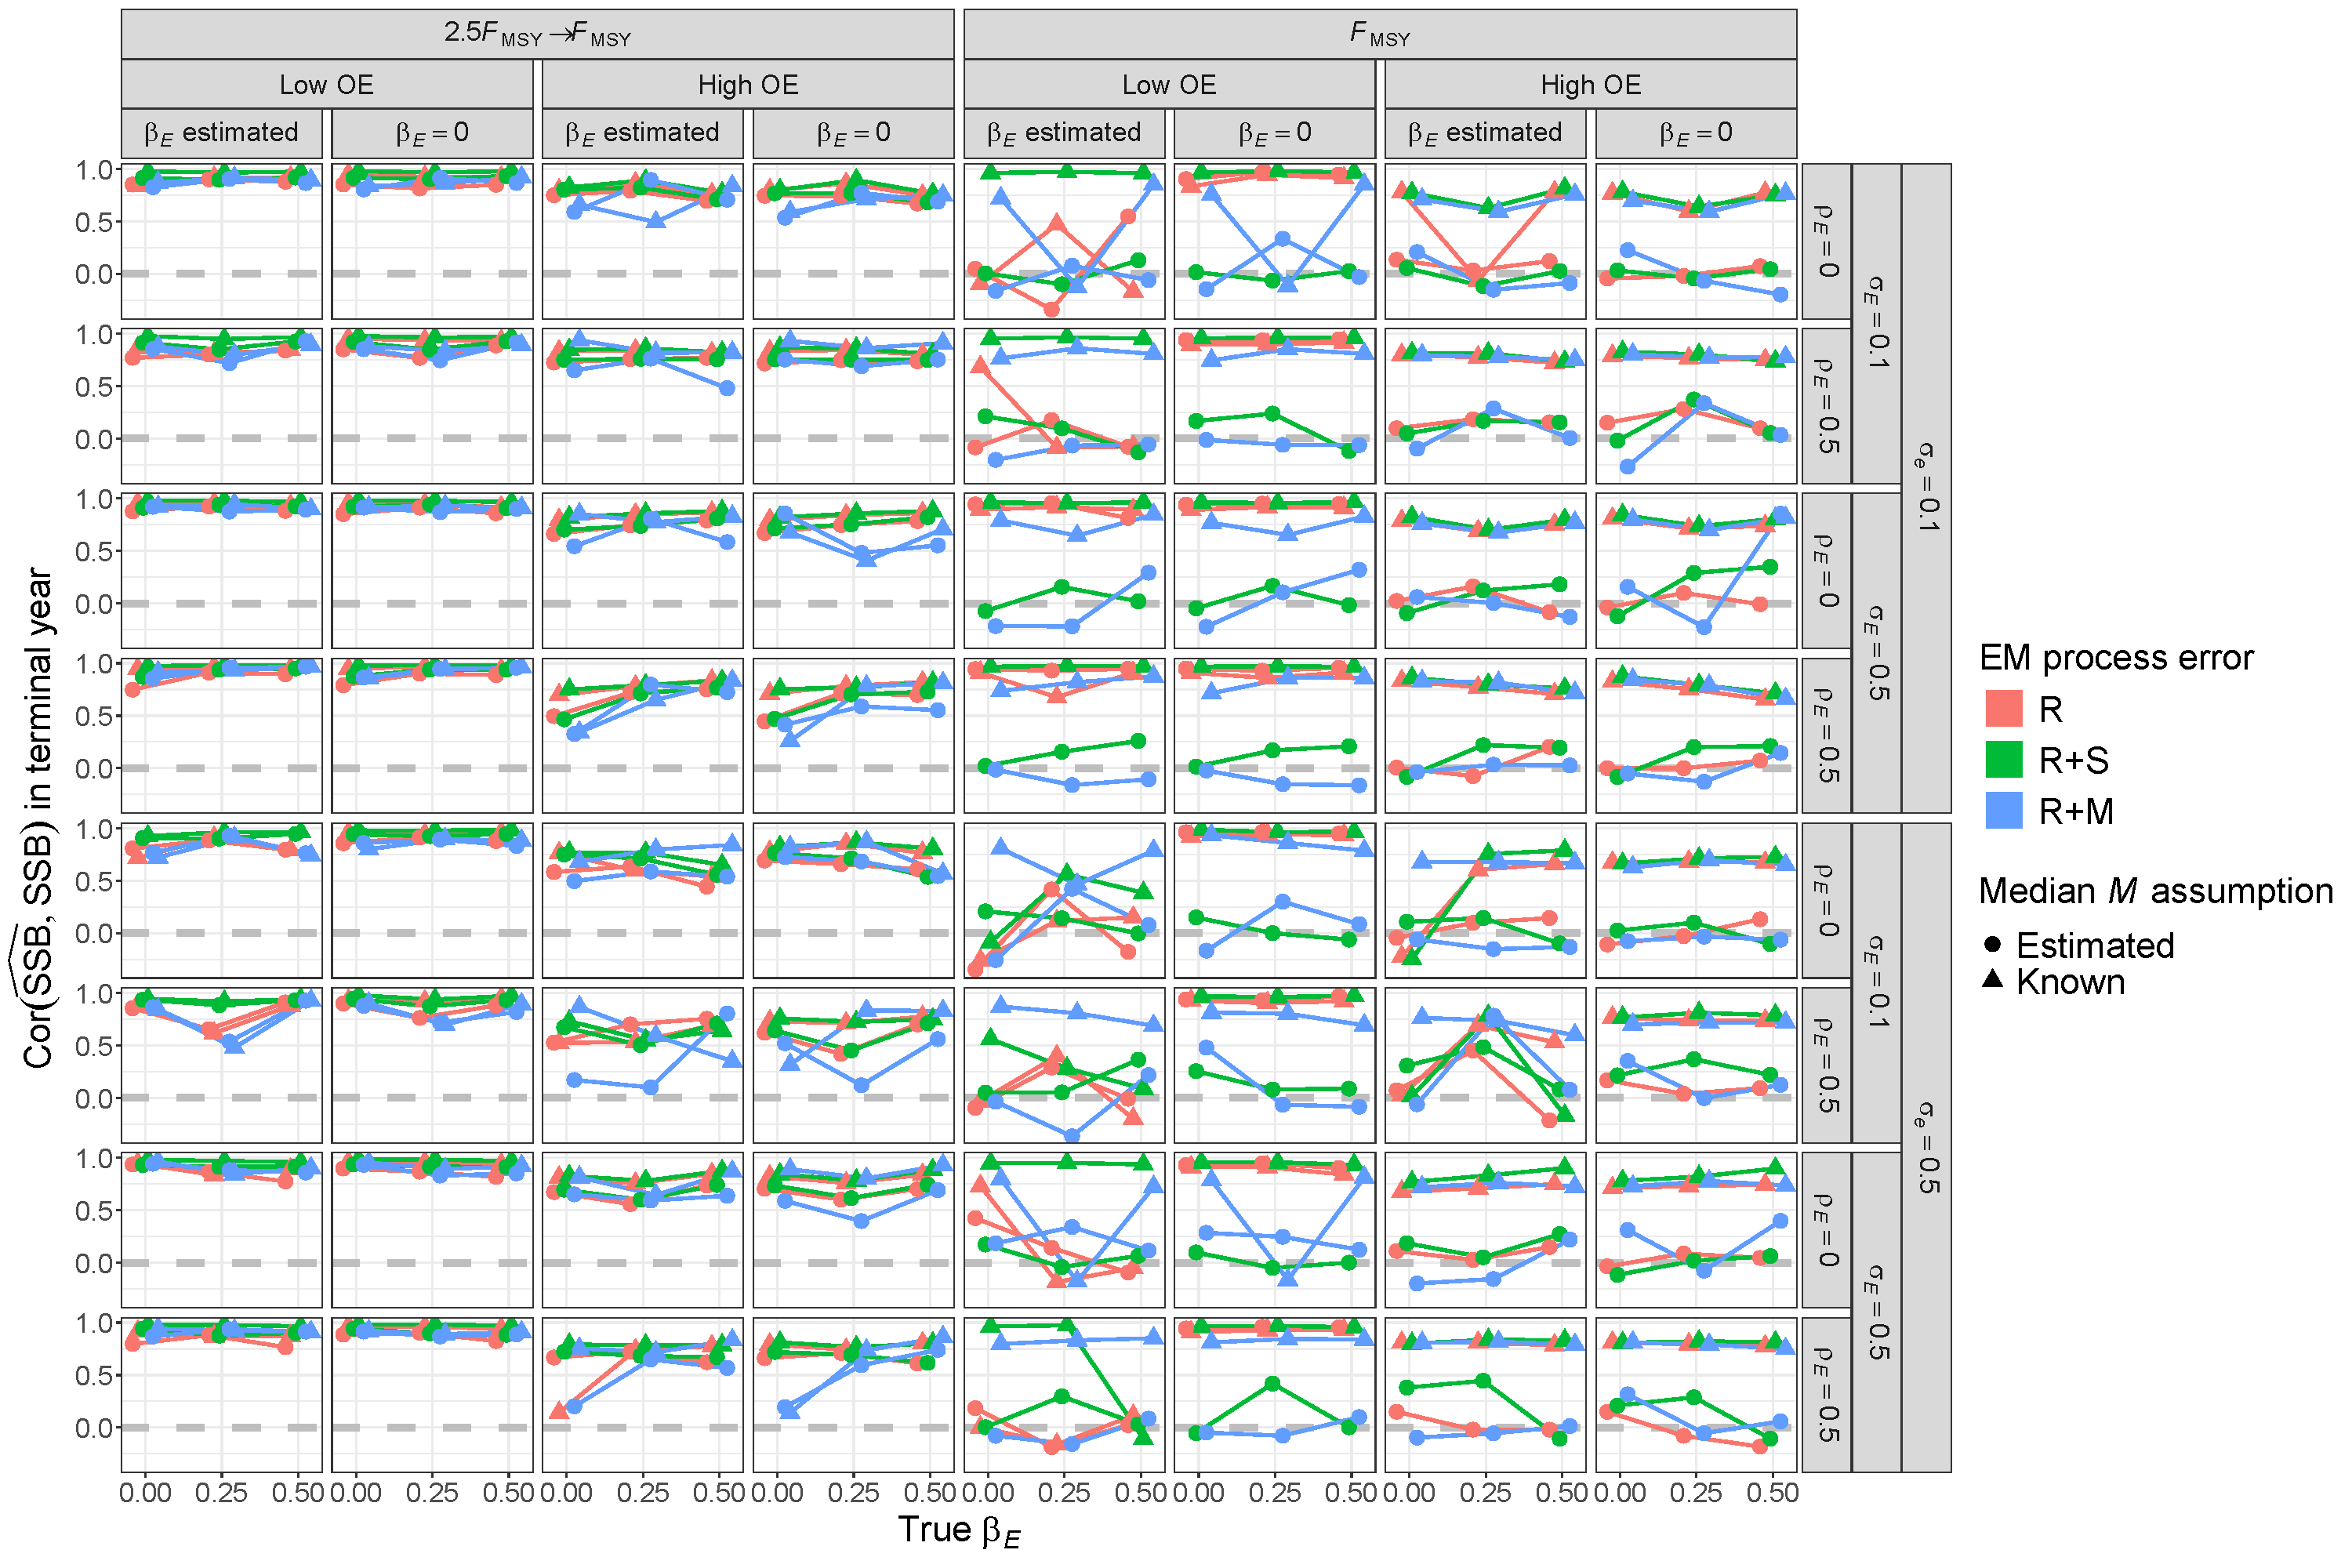
\includegraphics[height = \textheight]{terminal_year_ssb_corr_RSom}
%DIFDELCMD < \end{center}
%DIFDELCMD < %%%
%DIFDELCMD < \caption{%
{%DIFAUXCMD
\DIFdelFL{For R+S OMs, correlation of estimates and true values of terminal year SSB for EMs with alternative process error assumptions, treatment of covariate effect ($\beta_E = 0$ or estimated), and treatment of median $M$ parameter ($\beta_M$ estimated or known).}}%DIFAUXCMD
%DIFDELCMD < \label{terminal_ssb_corr_RSom}
%DIFDELCMD < \end{figure}
%DIFDELCMD < \end{landscape}
%DIFDELCMD < 

%DIFDELCMD < \begin{landscape}
%DIFDELCMD < \begin{figure}
%DIFDELCMD < \begin{center}
%DIFDELCMD < 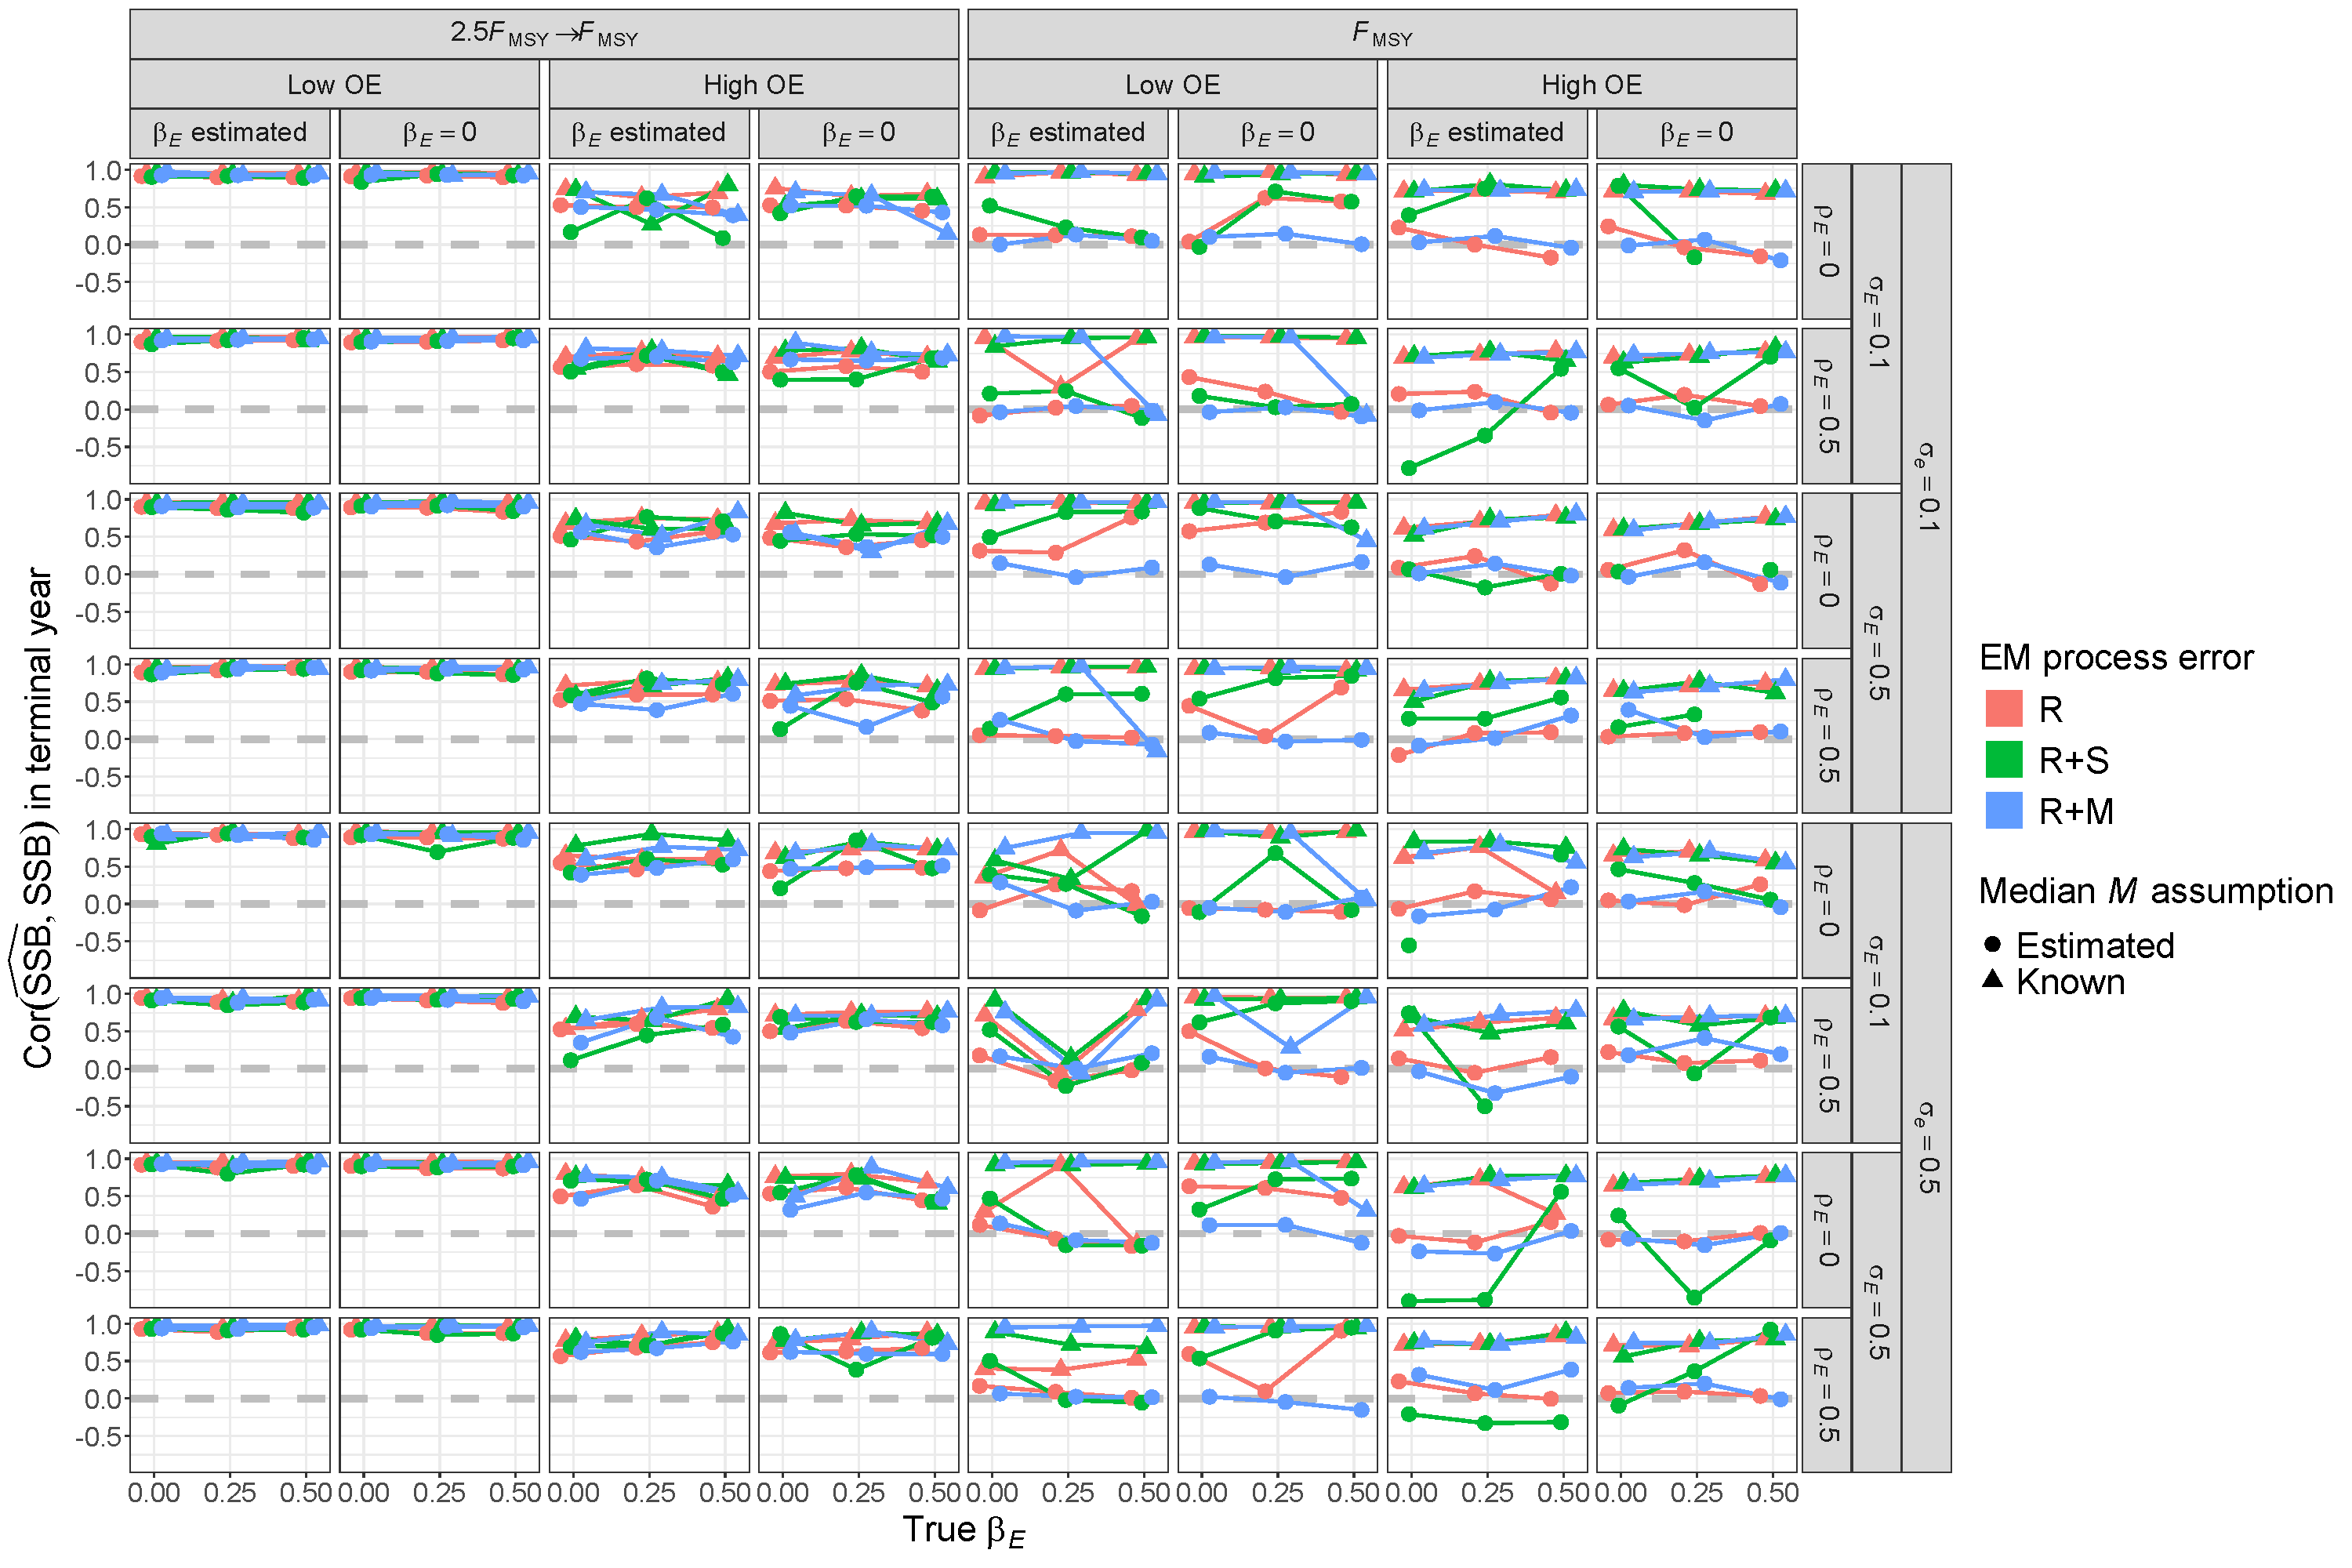
\includegraphics[height = \textheight]{terminal_year_ssb_corr_RMom}
%DIFDELCMD < \end{center}
%DIFDELCMD < %%%
%DIFDELCMD < \caption{%
{%DIFAUXCMD
\DIFdelFL{For R+M OMs, correlation of estimates and true vales of terminal year SSB for EMs with alternative process error assumptions, treatment of covariate effect ($\beta_E = 0$ or estimated), and treatment of median $M$ parameter ($\beta_M$ estimated or known).}}%DIFAUXCMD
%DIFDELCMD < \label{terminal_ssb_corr_RMom}
%DIFDELCMD < \end{figure}
%DIFDELCMD < \end{landscape}
%DIFDELCMD < 

%DIFDELCMD < %%%
\subsection*{\DIFdel{Terminal year fishing mortality bias}}%DIFAUXCMD
%DIFDELCMD < \label{terminal-year-fishing-mortality-bias}
%DIFDELCMD < %%%
\addcontentsline{toc}{subsection}{\DIFdel{Terminal year fishing mortality bias}}
%DIFAUXCMD
%DIFDELCMD < 

%DIFDELCMD < \begin{landscape}
%DIFDELCMD < \begin{figure}
%DIFDELCMD < \begin{center}
%DIFDELCMD < %%%
\DIFdelendFL 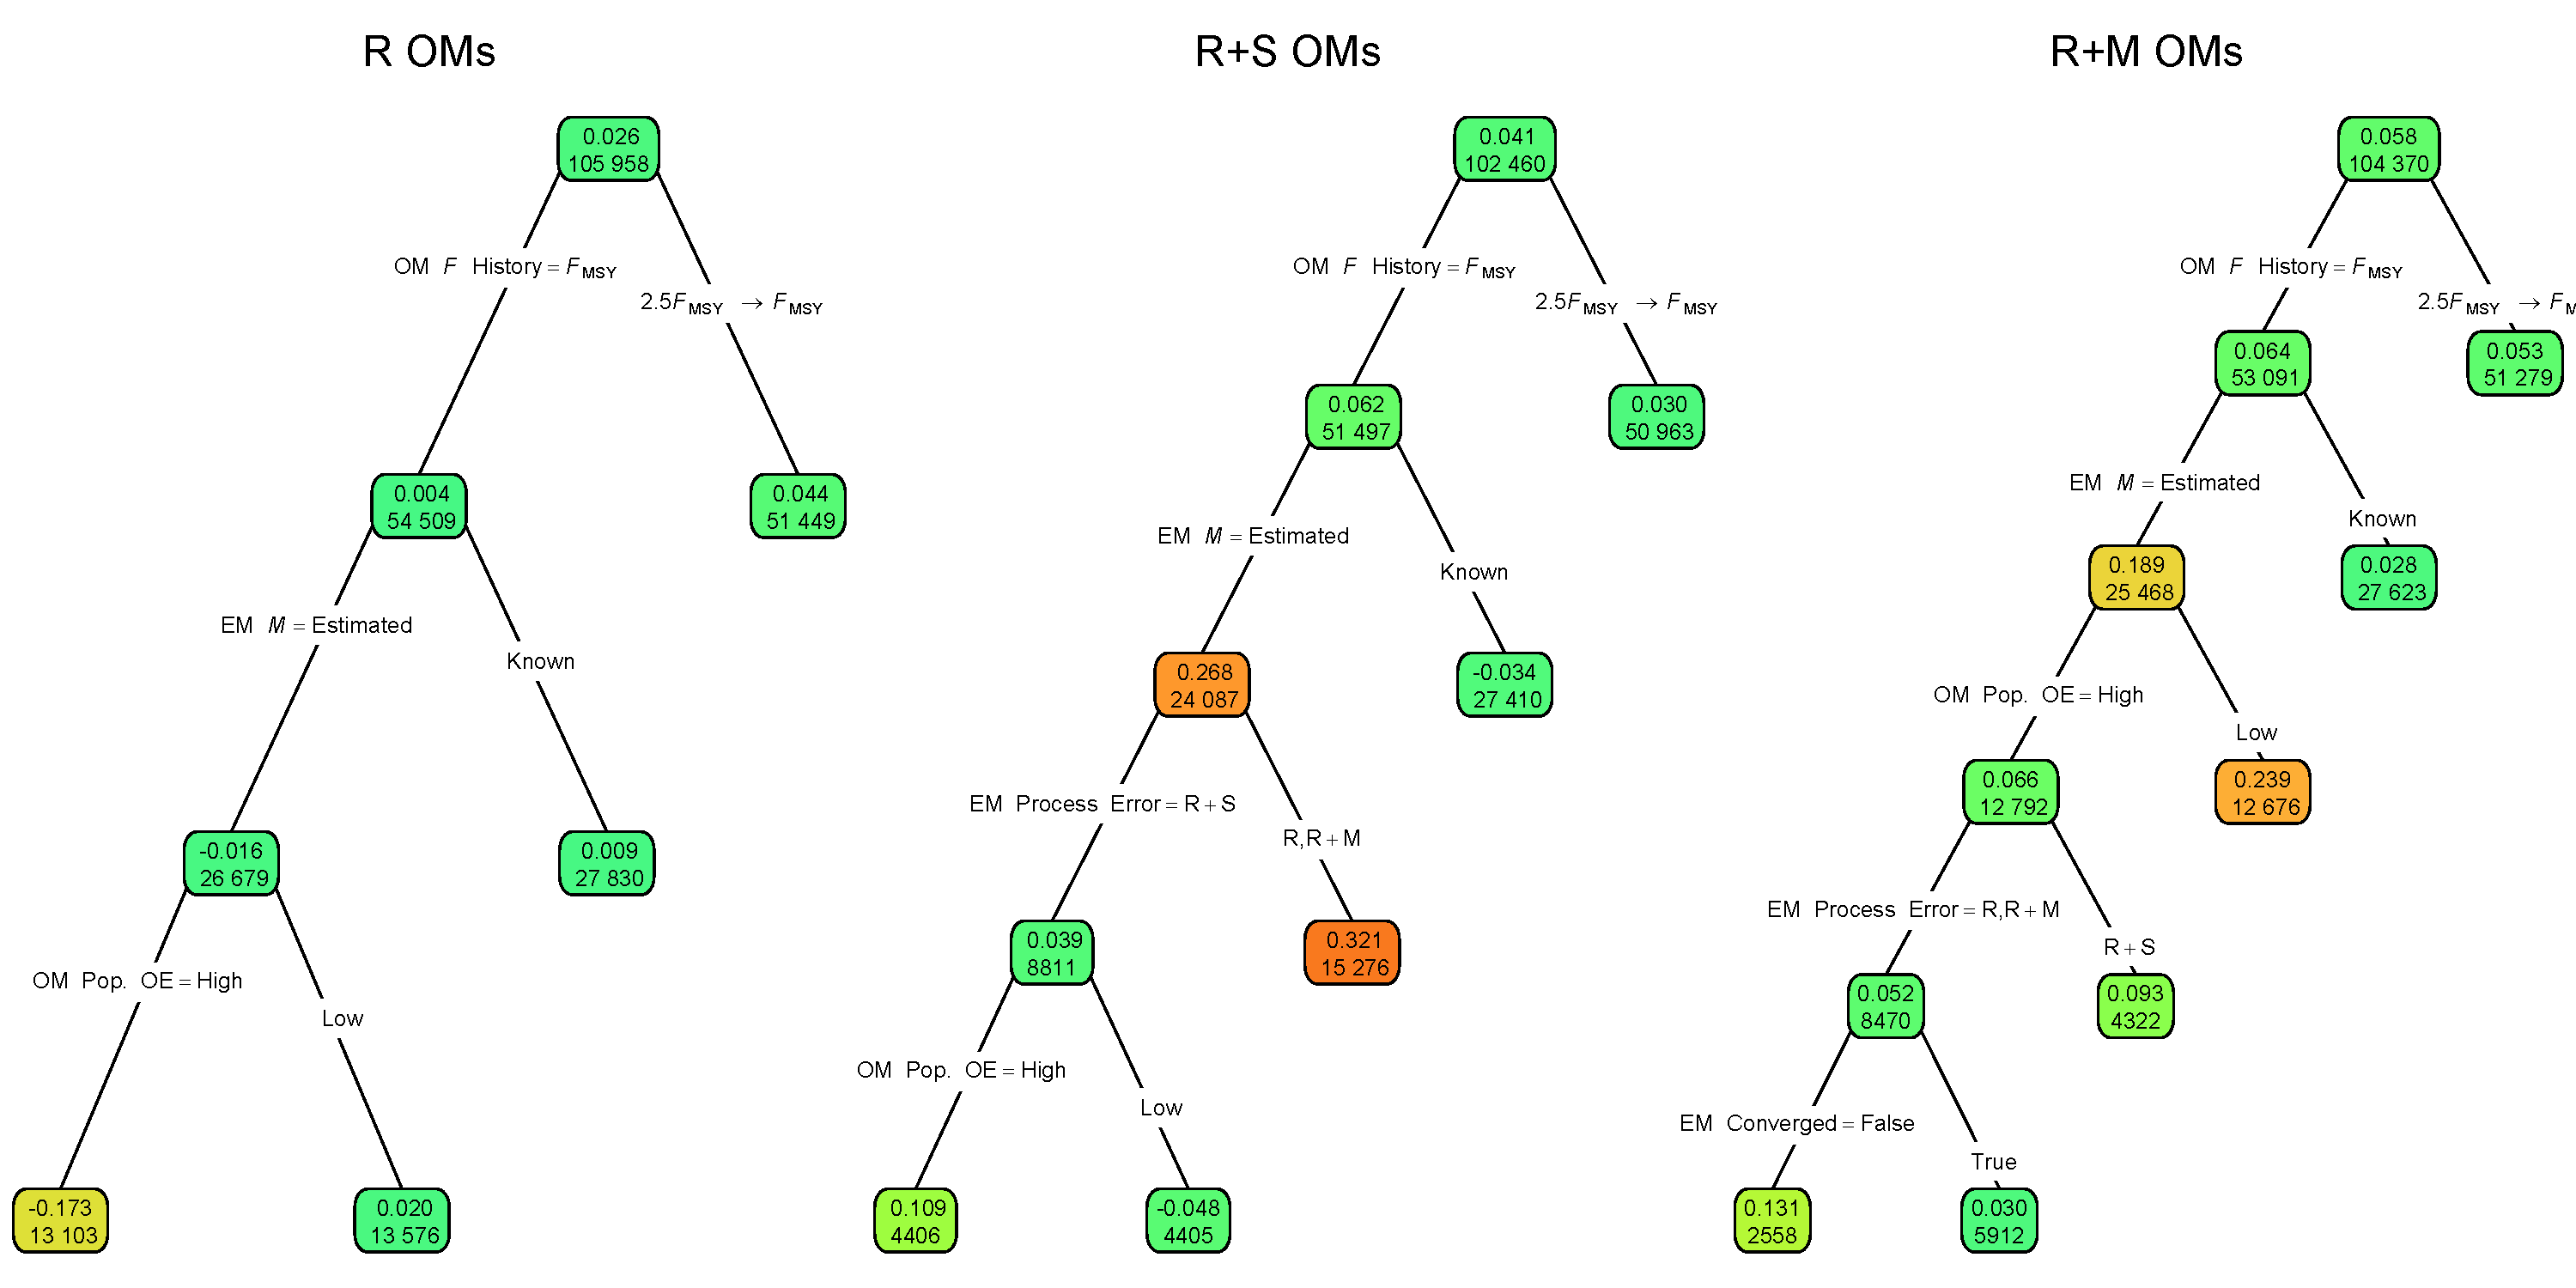
\includegraphics[width = 1.4\textwidth]{term_F_bias_regtree_plots}
\end{center}
\caption{Regression trees \DIFdelbeginFL \DIFdelFL{indicating primary factors determining reductions in sums of squares of errors in estimation measured by Eq. \ref{relerror_trans_response} }\DIFdelendFL for \DIFdelbeginFL \DIFdelFL{the }\DIFdelendFL \DIFaddbeginFL \DIFaddFL{errors }\DIFaddendFL terminal year fishing mortality rate \DIFdelbeginFL \DIFdelFL{in EMs fitted to operating models (OMs) with process error on recruitment only (R), recruitment and apparent survival (R+S), or recruitment and natural mortality (R+M)}\DIFdelendFL \DIFaddbeginFL \DIFaddFL{as measured by Eq}\DIFaddendFL . \DIFaddbeginFL \DIFaddFL{\ref{relerror_trans_response}. }\DIFaddendFL Each node shows the median error \DIFdelbeginFL \DIFdelFL{(top) and number of observations (bottom) }\DIFdelendFL for the corresponding subset. Lower or higher \DIFdelbeginFL \DIFdelFL{median }\DIFdelendFL absolute \DIFaddbeginFL \DIFaddFL{median }\DIFaddendFL errors \DIFdelbeginFL \DIFdelFL{of the process error assumption }\DIFdelendFL are indicated by more green or red polygons, respectively. \DIFaddbeginFL \DIFaddFL{See Figure \ref{conv_class} caption and Table \ref{factor_table} for further details.}\DIFaddendFL }\label{term_F_bias_regtree}
\end{figure}
\end{landscape}

\begin{table}
\caption{Percent reduction in deviance for linear regression models fit to errors in \DIFdelbeginFL \DIFdelFL{estimation }\DIFdelendFL \DIFaddbeginFL \DIFaddFL{terminal year fishing mortality rate as }\DIFaddendFL measured by Eq. \ref{relerror_trans_response}\DIFdelbeginFL \DIFdelFL{for the terminal year fishing mortality rates}\DIFdelendFL . \DIFdelbeginFL \DIFdelFL{Table rows give each operating model (OM) }\DIFdelendFL \DIFaddbeginFL \DIFaddFL{See Tables \ref{convergence_PRD_table} }\DIFaddendFL and \DIFdelbeginFL \DIFdelFL{estimating model (EM) factor included individually, combined, and with second and third order interactions}\DIFdelendFL \DIFaddbeginFL \DIFaddFL{\ref{factor_table} for further details}\DIFaddendFL .\DIFdelbeginFL \DIFdelFL{Table columns are operating models (OMs) with process error on recruitment only (R), recruitment and apparent survival (R+S), or recruitment and natural mortality (R+M).}\DIFdelendFL }\label{bias_F_PRD_table}
{\begin{center}
\begin{tabular}{lrrr}
\hline\hline
\multicolumn{1}{l}{Factor}&\multicolumn{1}{c}{R}&\multicolumn{1}{c}{R+S}&\multicolumn{1}{c}{R+M}\tabularnewline
\hline
Convergence&\textless  0.01& 0.19& 0.01\tabularnewline
OM $F$ history& 1.92& 2.42& 1.94\tabularnewline
OM Obs. Error& 0.74& 0.12& 1.12\tabularnewline
OM $\sigma_e$& 0.01&\textless  0.01&\textless  0.01\tabularnewline
OM $\sigma_E$&\textless  0.01&\textless  0.01&\textless  0.01\tabularnewline
OM $\rho_{E}$&\textless  0.01&\textless  0.01&\textless  0.01\tabularnewline
OM $\beta_{E}$&\textless  0.01& 0.01&\textless  0.01\tabularnewline
EM Process Error& 0.40& 0.92& 0.48\tabularnewline
EM $\beta_{E}$ assumption& 0.01& 0.03& 0.02\tabularnewline
EM $M$ assumption& 1.58& 1.85& 1.68\tabularnewline
All factors& 4.95& 5.82& 5.35\tabularnewline
+ All Two Way&10.91&11.03&12.23\tabularnewline
+ All Three Way&14.16&13.24&16.19\tabularnewline
\hline
\end{tabular}\end{center}
}
\end{table}

\begin{landscape}
\begin{figure}
\begin{center}
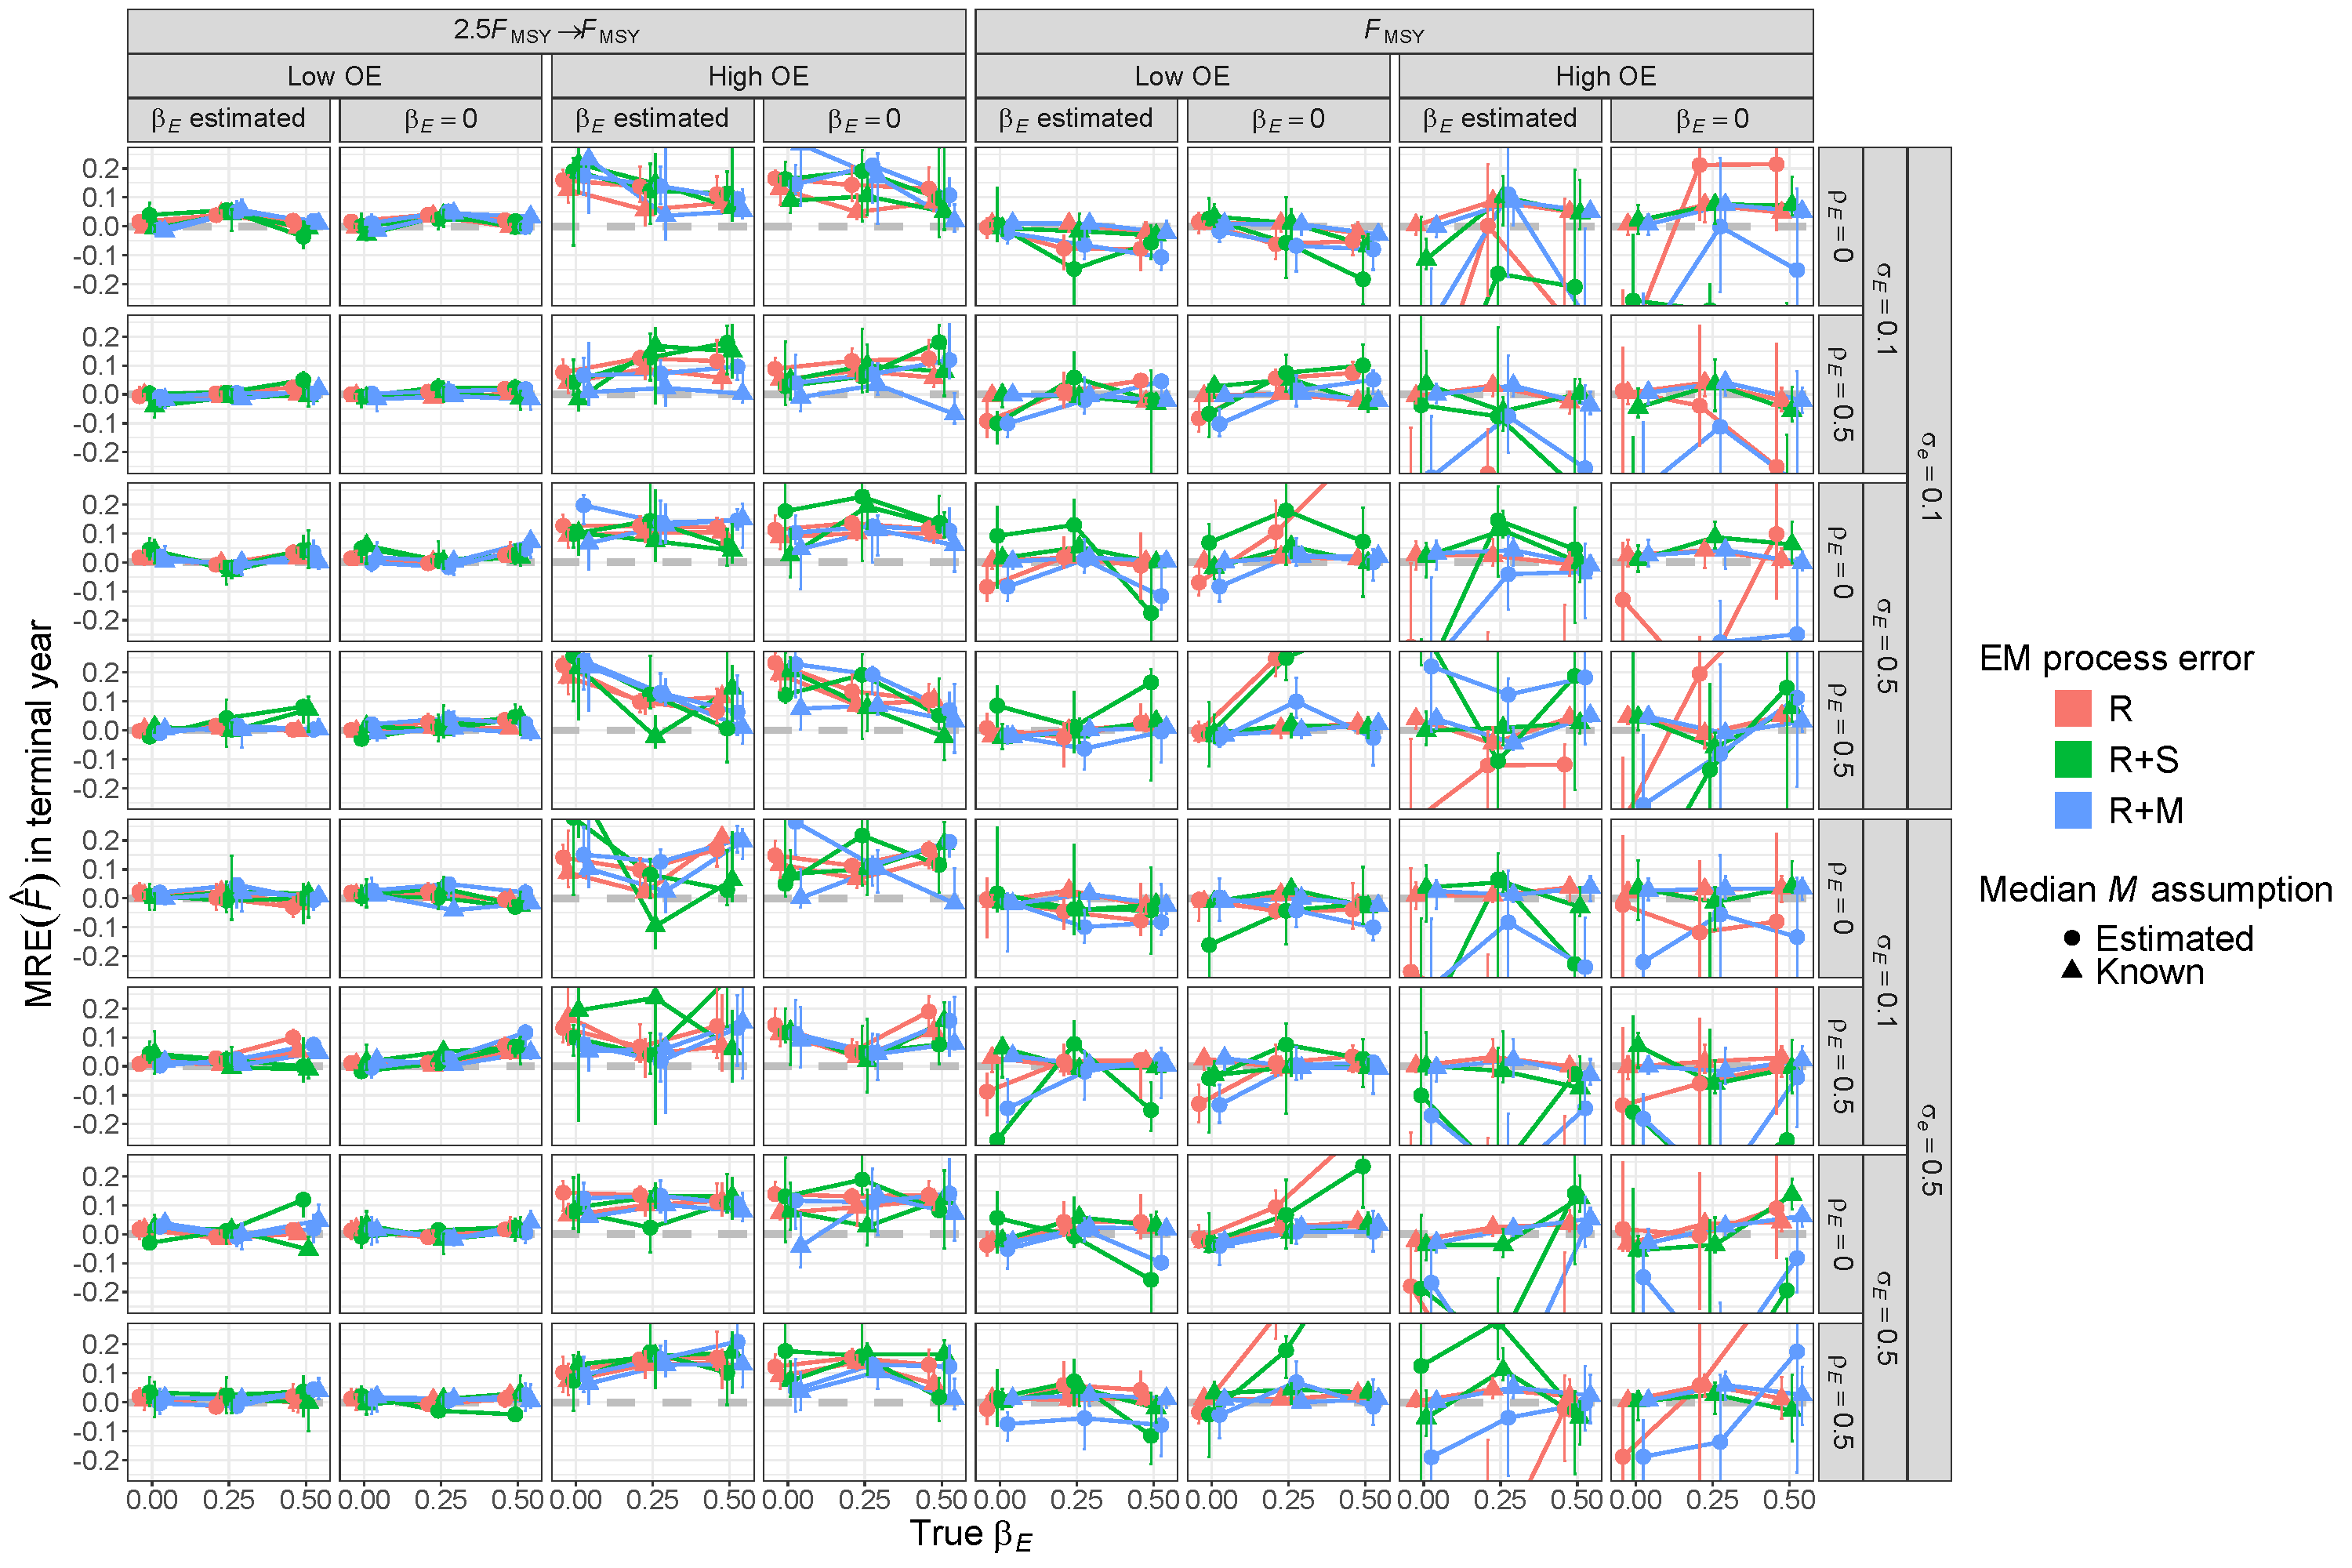
\includegraphics[height = \textheight]{terminal_year_F_bias_Rom}
\end{center}
\caption{For R \DIFdelbeginFL \DIFdelFL{OMs}\DIFdelendFL \DIFaddbeginFL \DIFaddFL{operating models}\DIFaddendFL , median relative error (MRE) of estimates of fully-selected fishing mortality ($F$) in the terminal year for \DIFdelbeginFL \DIFdelFL{EMs }\DIFdelendFL \DIFaddbeginFL \DIFaddFL{estimating models }\DIFaddendFL with alternative process error assumptions, treatment of covariate effect ($\beta_E = 0$ or estimated), and treatment of median $M$ parameter ($\beta_M$ estimated or known).\DIFdelbeginFL \DIFdelFL{All OMs had low observation error and contrast in fishing mortality.}\DIFdelendFL }\label{terminal_F_bias_Rom}
\end{figure}
\end{landscape}

\begin{landscape}
\begin{figure}
\begin{center}
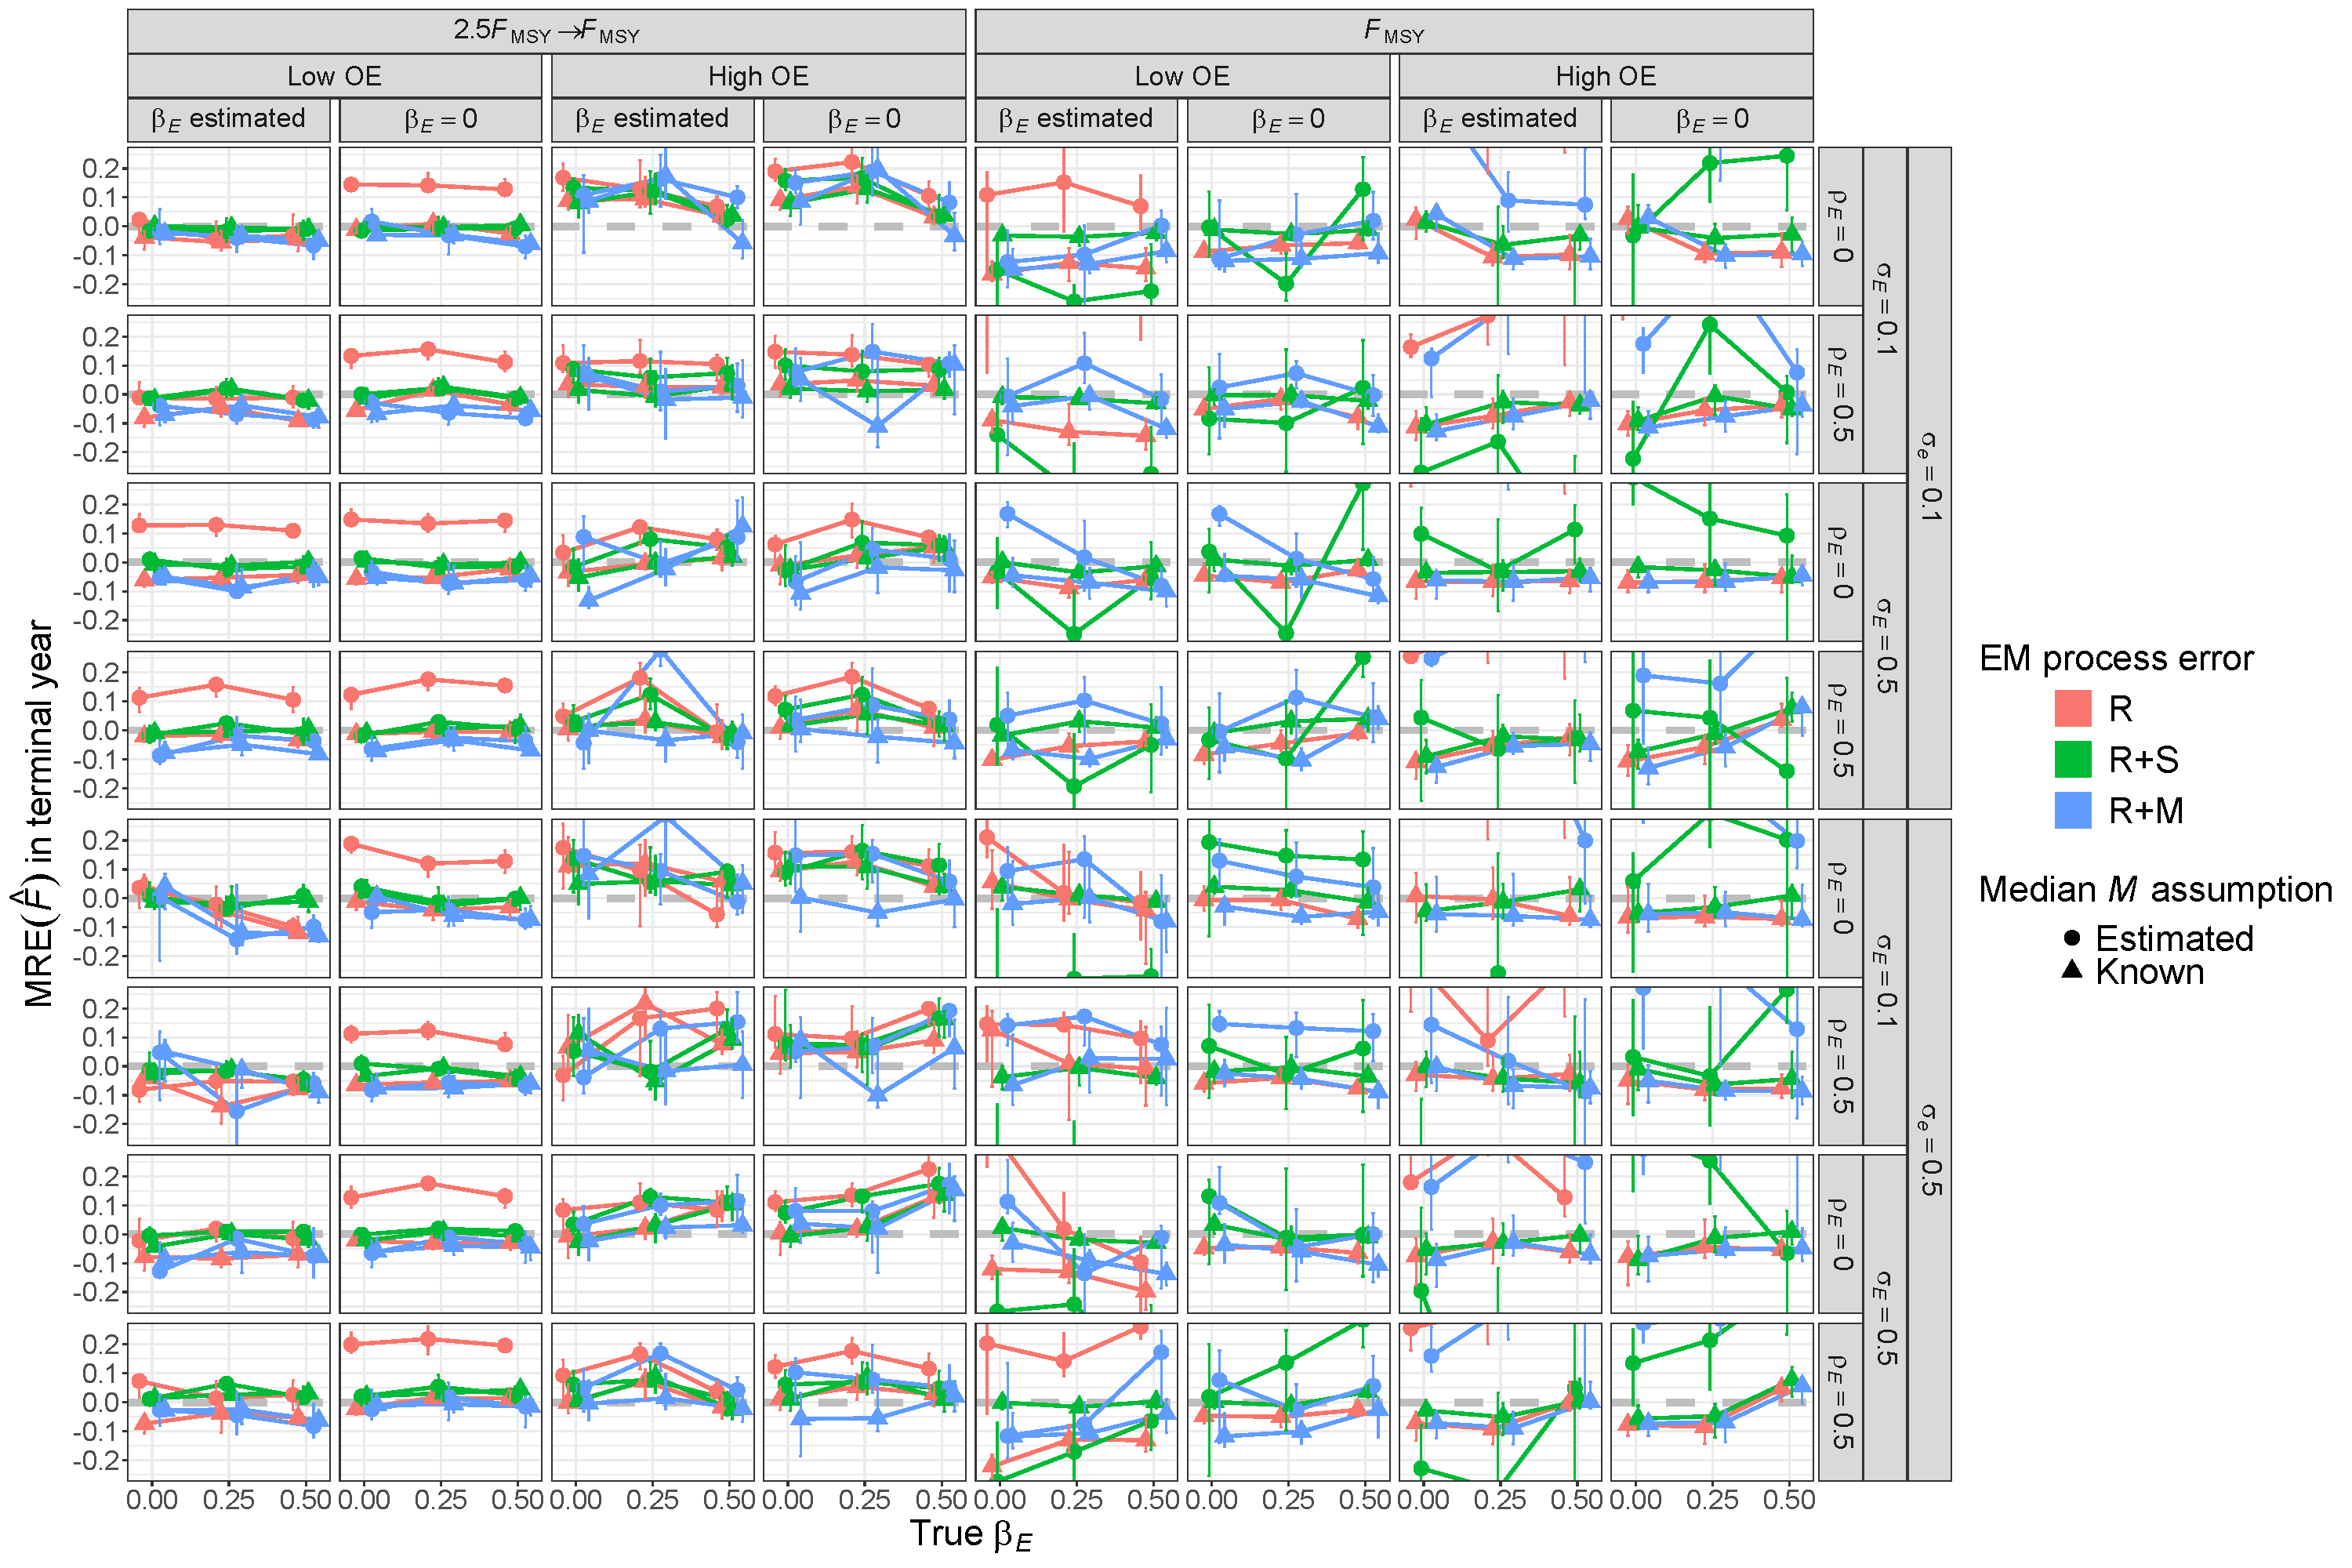
\includegraphics[height = \textheight]{terminal_year_F_bias_RSom}
\end{center}
\caption{For R+S \DIFdelbeginFL \DIFdelFL{OMs}\DIFdelendFL \DIFaddbeginFL \DIFaddFL{operating models}\DIFaddendFL , median relative error (MRE) of estimates of fully-selected fishing mortality ($F$) in the terminal year for \DIFdelbeginFL \DIFdelFL{EMs }\DIFdelendFL \DIFaddbeginFL \DIFaddFL{estimating models }\DIFaddendFL with alternative process error assumptions, treatment of covariate effect ($\beta_E = 0$ or estimated), and treatment of median $M$ parameter ($\beta_M$ estimated or known).\DIFdelbeginFL \DIFdelFL{All OMs had low observation error and contrast in fishing mortality.}\DIFdelendFL }\label{terminal_F_bias_RSom}
\end{figure}
\end{landscape}

\begin{landscape}
\begin{figure}
\begin{center}
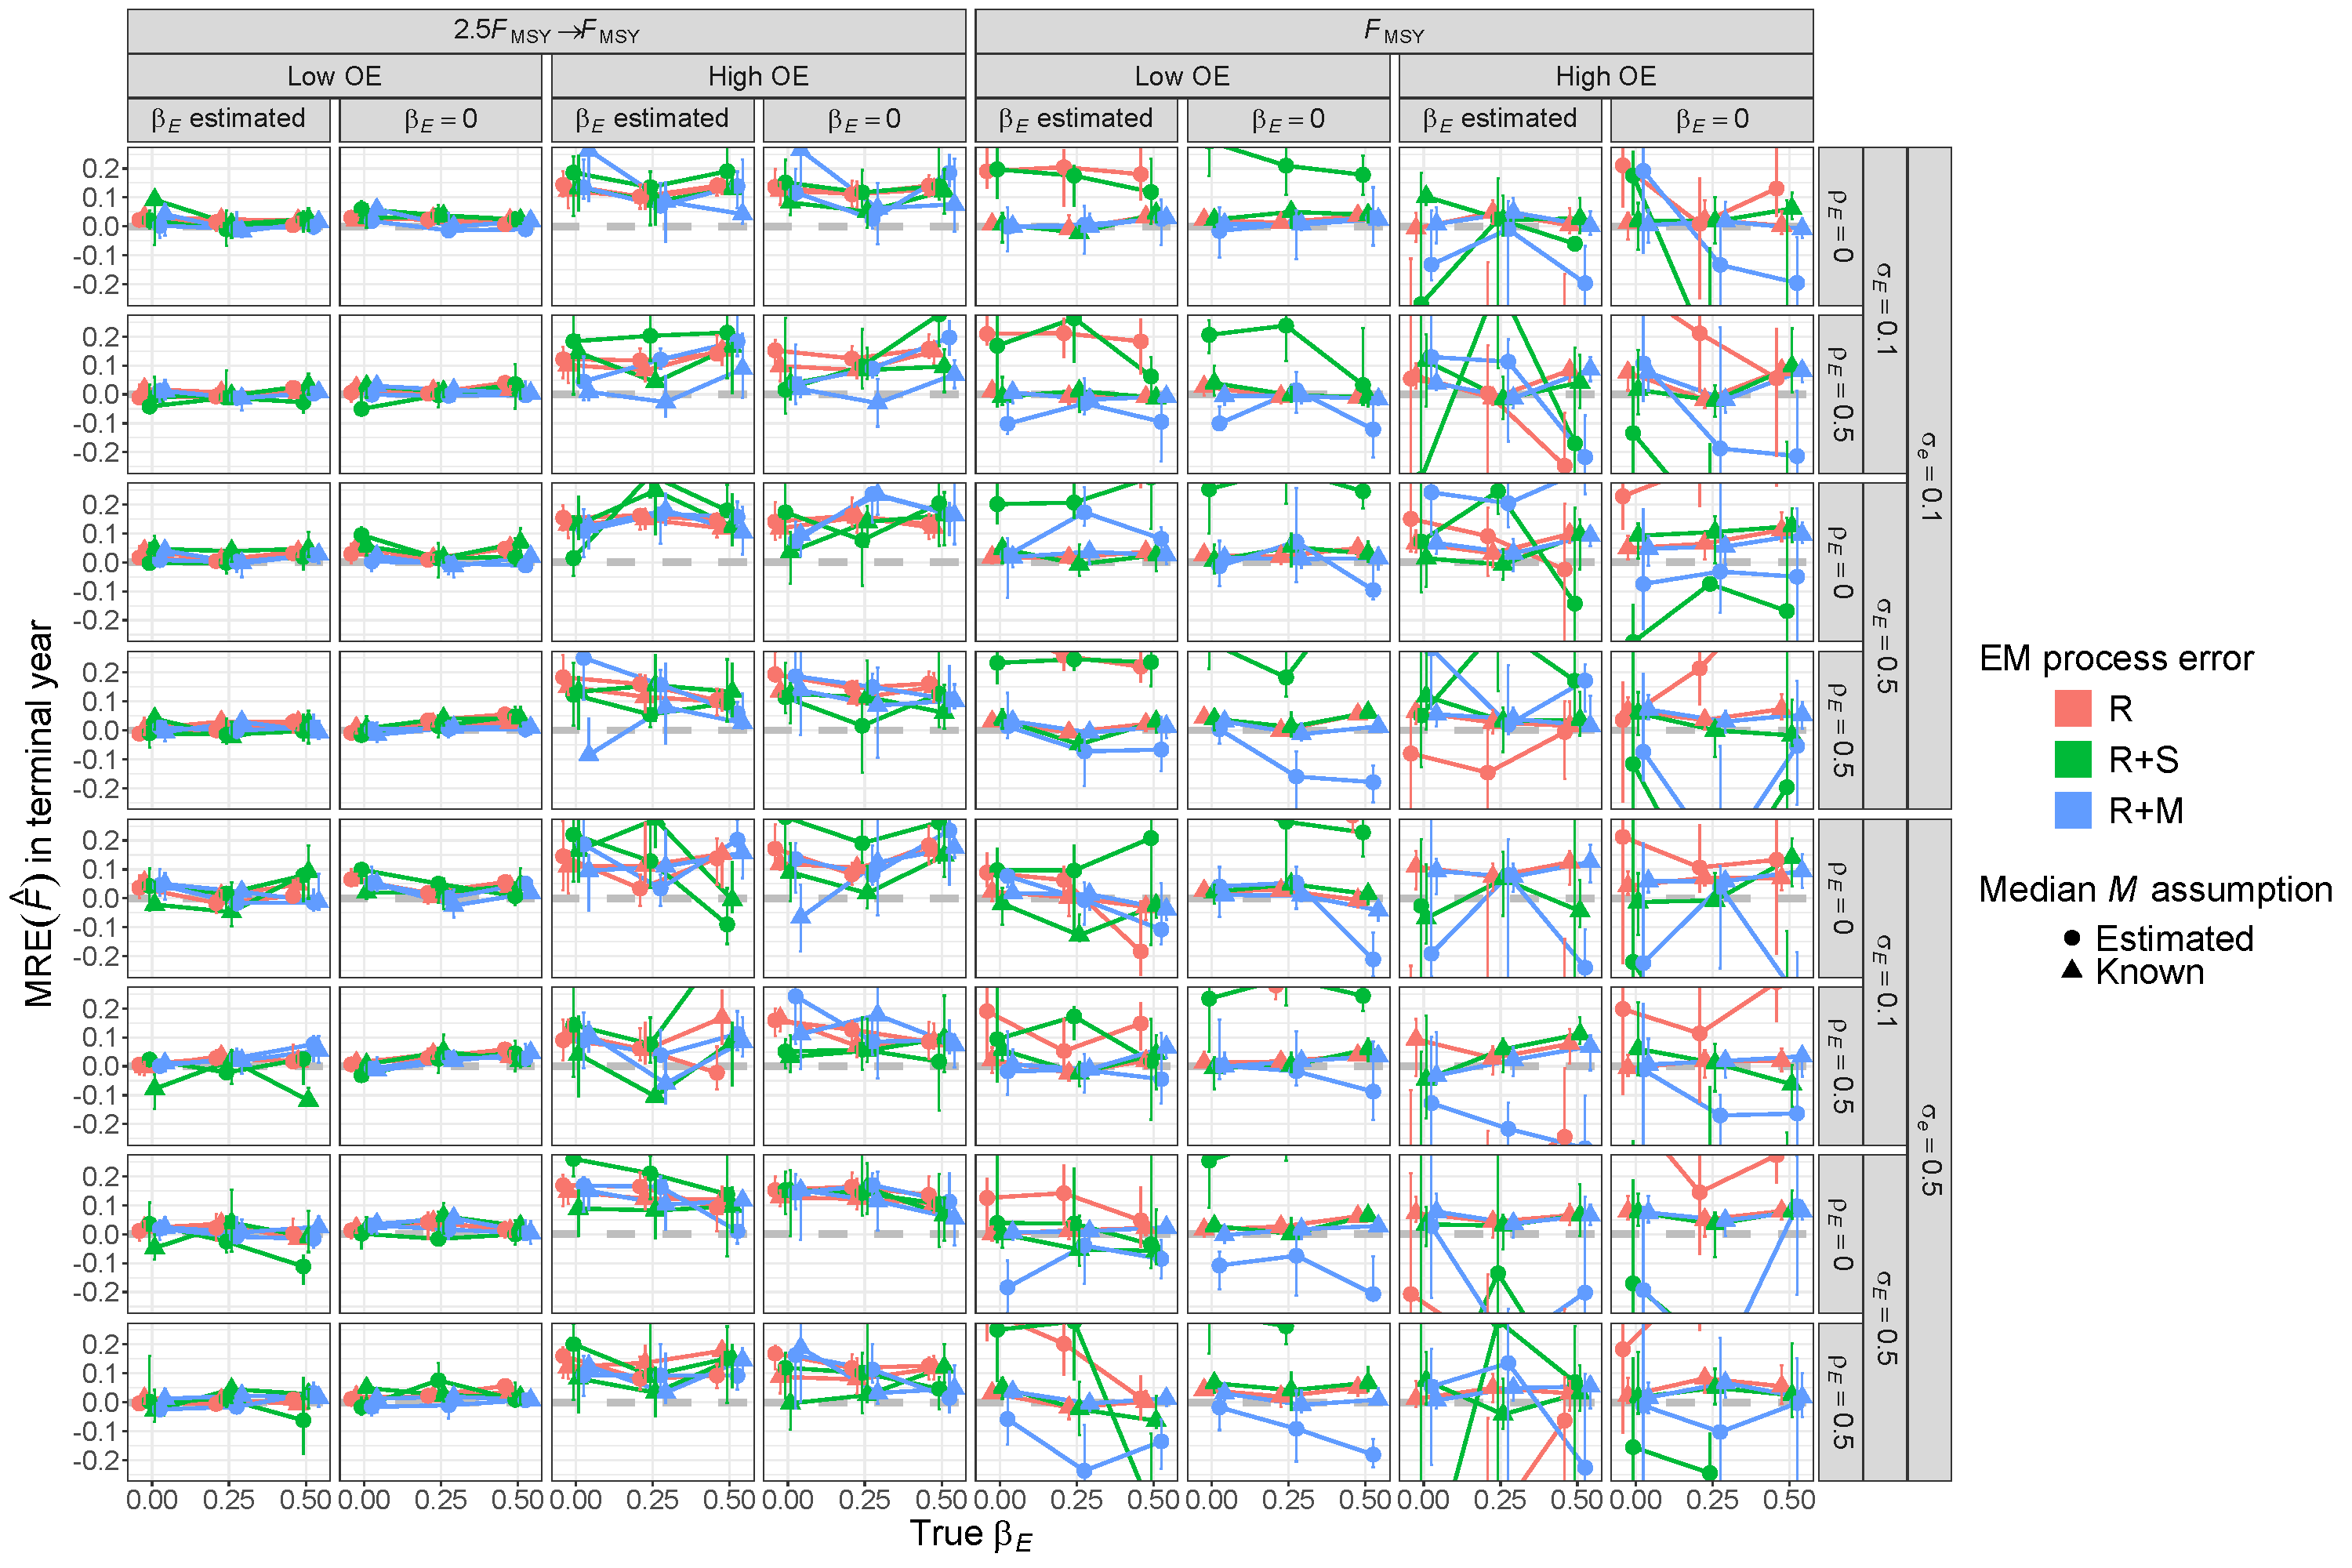
\includegraphics[height = \textheight]{terminal_year_F_bias_RMom}
\end{center}
\caption{For R+M \DIFdelbeginFL \DIFdelFL{OMs}\DIFdelendFL \DIFaddbeginFL \DIFaddFL{operating models}\DIFaddendFL , median relative error (MRE) of estimates of fully-selected fishing mortality ($F$) in the terminal year for \DIFdelbeginFL \DIFdelFL{EMs }\DIFdelendFL \DIFaddbeginFL \DIFaddFL{estimating models }\DIFaddendFL with alternative process error assumptions, treatment of covariate effect ($\beta_E = 0$ or estimated), and treatment of median $M$ parameter ($\beta_M$ estimated or known).\DIFdelbeginFL \DIFdelFL{All OMs had low observation error and contrast in fishing mortality.}\DIFdelendFL }\label{terminal_F_bias_RMom}
\end{figure}
\end{landscape}

\DIFdelbegin \subsection*{\DIFdel{Terminal year fishing mortality accuracy}}%DIFAUXCMD
%DIFDELCMD < \label{terminal-year-fishing-mortality-accuracy}
%DIFDELCMD < %%%
\addcontentsline{toc}{subsection}{\DIFdel{Terminal year fishing mortality accuracy}}
%DIFAUXCMD
%DIFDELCMD < 

%DIFDELCMD < %%%
\DIFdelend \begin{landscape}
\begin{figure}
\begin{center}
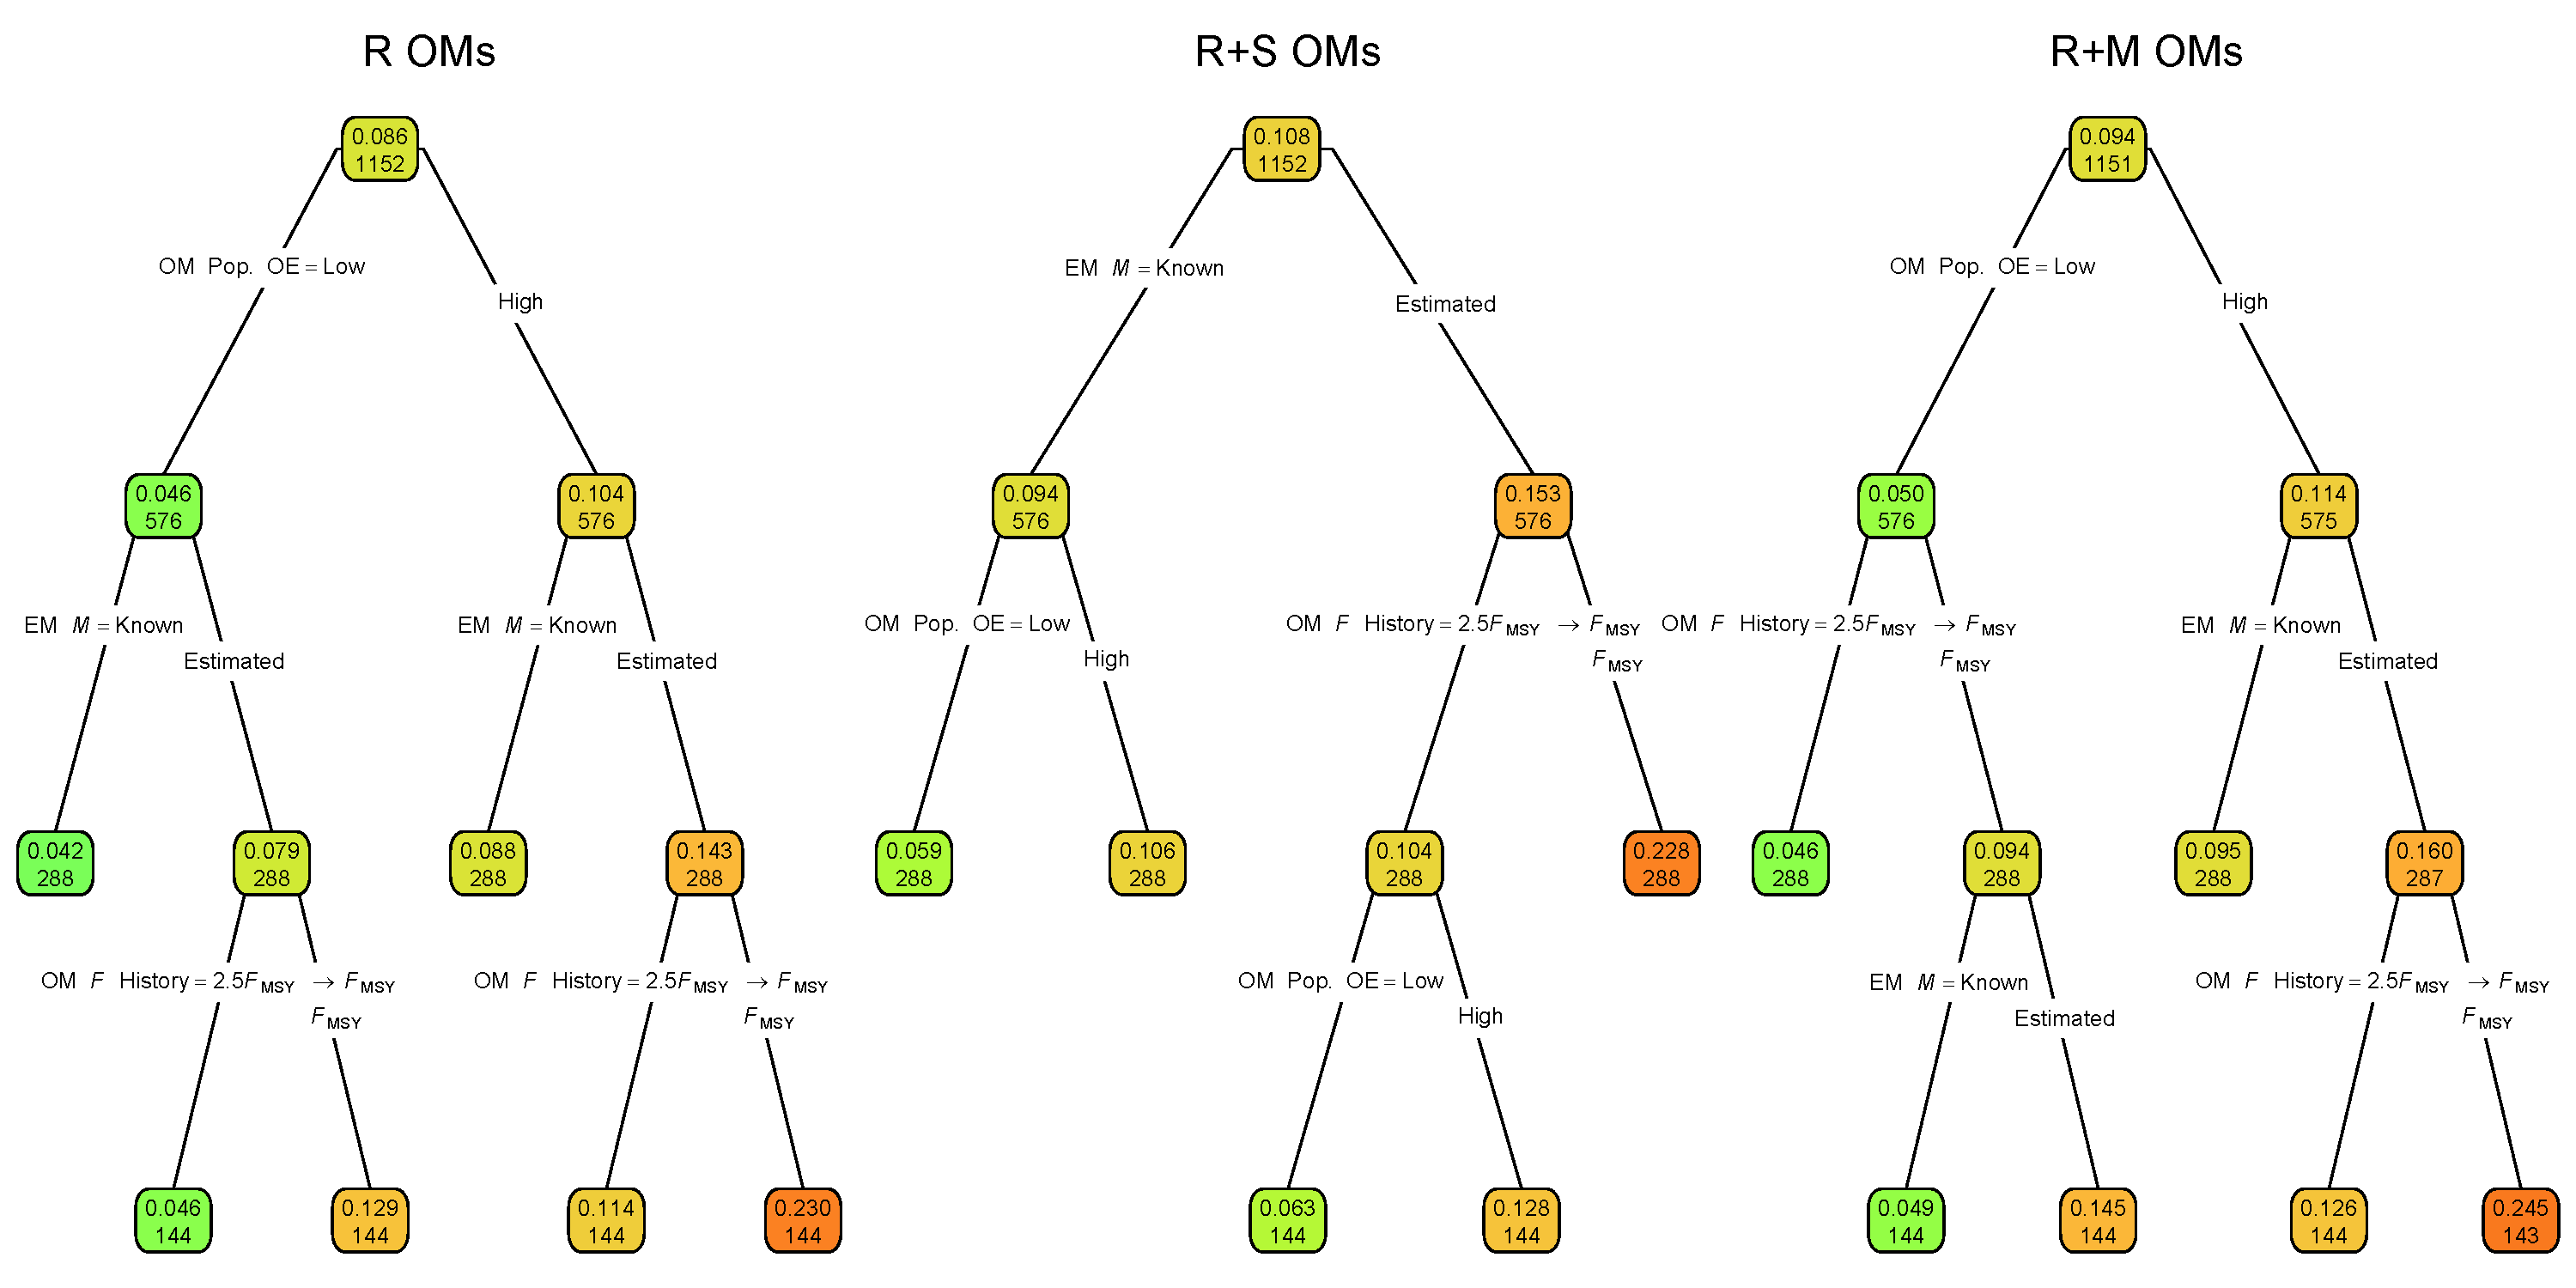
\includegraphics[width = 1.4\textwidth]{term_F_rmse_regtree_plots}
\end{center}
\caption{Regression trees \DIFdelbeginFL \DIFdelFL{indicating primary factors determining reductions in sums of squares of errors }\DIFdelendFL for the log-transformed RMSE of terminal year fishing mortality rate\DIFdelbeginFL \DIFdelFL{in EMs fitted to operating models (OMs) with process error on recruitment only (R), recruitment and apparent survival (R+S), or recruitment and natural mortality (R+M)}\DIFdelendFL . Each node shows the median error \DIFdelbeginFL \DIFdelFL{(top) and number of observations (bottom) }\DIFdelendFL for the corresponding subset. Lower or higher median RMSE \DIFdelbeginFL \DIFdelFL{are }\DIFdelendFL \DIFaddbeginFL \DIFaddFL{is }\DIFaddendFL indicated by more green or red polygons, respectively. \DIFaddbeginFL \DIFaddFL{See Figure \ref{conv_class} caption and Table \ref{factor_table} for further details.}\DIFaddendFL }\label{term_F_rmse_regtree}
\end{figure}
\end{landscape}

\begin{table}
\caption{Percent reduction in deviance for linear regression models fit to log-transformed RMSE of terminal year fishing mortality rate. \DIFdelbeginFL \DIFdelFL{Table rows give each operating model (OM) }\DIFdelendFL \DIFaddbeginFL \DIFaddFL{See Tables \ref{convergence_PRD_table} }\DIFaddendFL and \DIFdelbeginFL \DIFdelFL{estimating model (EM) factor included individually, combined, and with second and third order interactions}\DIFdelendFL \DIFaddbeginFL \DIFaddFL{\ref{factor_table} for further details}\DIFaddendFL .\DIFdelbeginFL \DIFdelFL{Table columns are operating models (OMs) with process error on recruitment only (R), recruitment and apparent survival (R+S), or recruitment and natural mortality (R+M).}\DIFdelendFL }\label{rmse_F_PRD_table}
{\begin{center}
\begin{tabular}{lrrr}
\hline\hline
\multicolumn{1}{l}{Factor}&\multicolumn{1}{c}{R}&\multicolumn{1}{c}{R+S}&\multicolumn{1}{c}{R+M}\tabularnewline
\hline
OM $F$ history&11.29&25.63&13.46\tabularnewline
OM Obs. Error&37.27&21.42&35.47\tabularnewline
OM $\sigma_e$&\textless  0.01& 0.02& 0.02\tabularnewline
OM $\sigma_E$& 0.09& 0.03& 0.14\tabularnewline
OM $\rho_{E}$& 0.02& 0.01& 0.04\tabularnewline
OM $\beta_{E}$& 0.15& 0.03& 0.21\tabularnewline
EM Process Error& 0.42& 0.75& 0.63\tabularnewline
$EM \beta_{E}$ assumption& 0.04&\textless  0.01& 0.04\tabularnewline
EM $M$ assumption&25.38&26.10&24.68\tabularnewline
All factors&74.65&73.99&74.76\tabularnewline
+ All Two Way&92.28&91.29&91.64\tabularnewline
+ All Three Way&94.31&95.51&93.73\tabularnewline
\hline
\end{tabular}\end{center}
}
\end{table}
\pagebreak

\begin{landscape}
\begin{figure}
\begin{center}
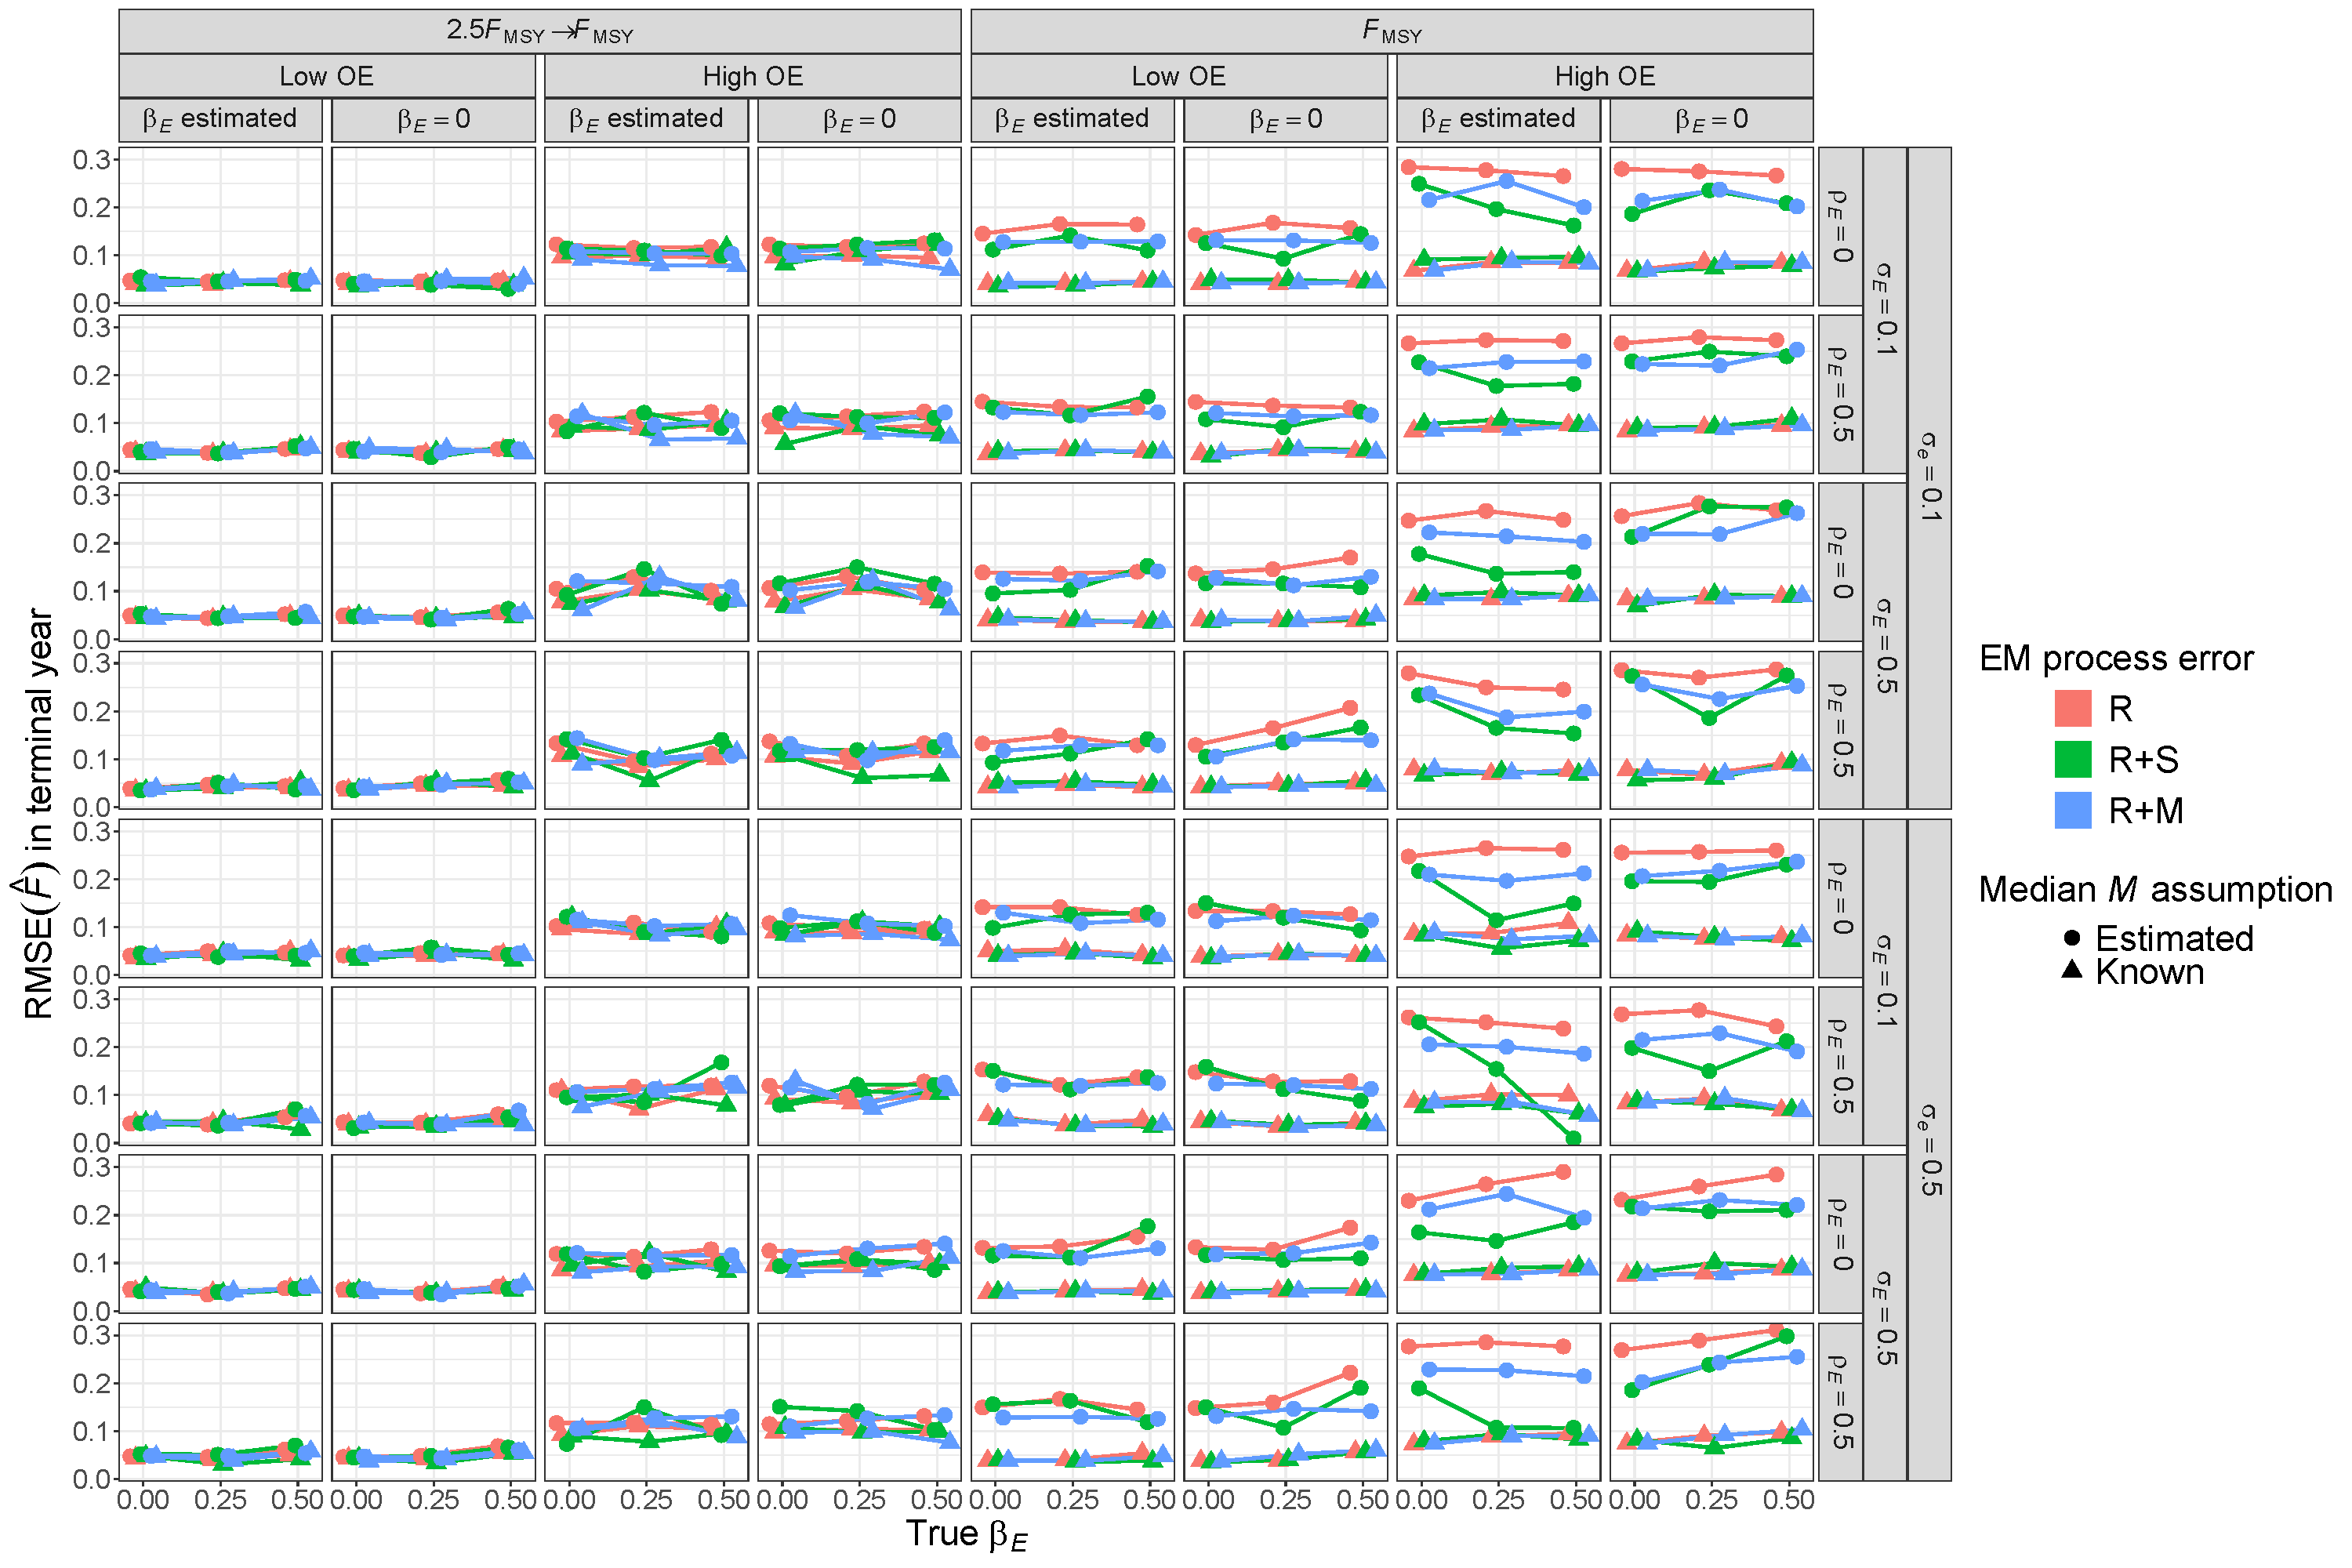
\includegraphics[height = \textheight]{terminal_year_F_rmse_Rom}
\end{center}
\caption{For R \DIFdelbeginFL \DIFdelFL{OMs}\DIFdelendFL \DIFaddbeginFL \DIFaddFL{operating models}\DIFaddendFL , RMSE of estimates of fully-selected fishing mortality ($F$)  in the terminal year for \DIFdelbeginFL \DIFdelFL{EMs }\DIFdelendFL \DIFaddbeginFL \DIFaddFL{estimating models }\DIFaddendFL with alternative process error assumptions, treatment of covariate effect ($\beta_E = 0$ or estimated), and treatment of median $M$ parameter ($\beta_M$ estimated or known).}\label{terminal_F_rmse_Rom}
\end{figure}
\end{landscape}

\begin{landscape}
\begin{figure}
\begin{center}
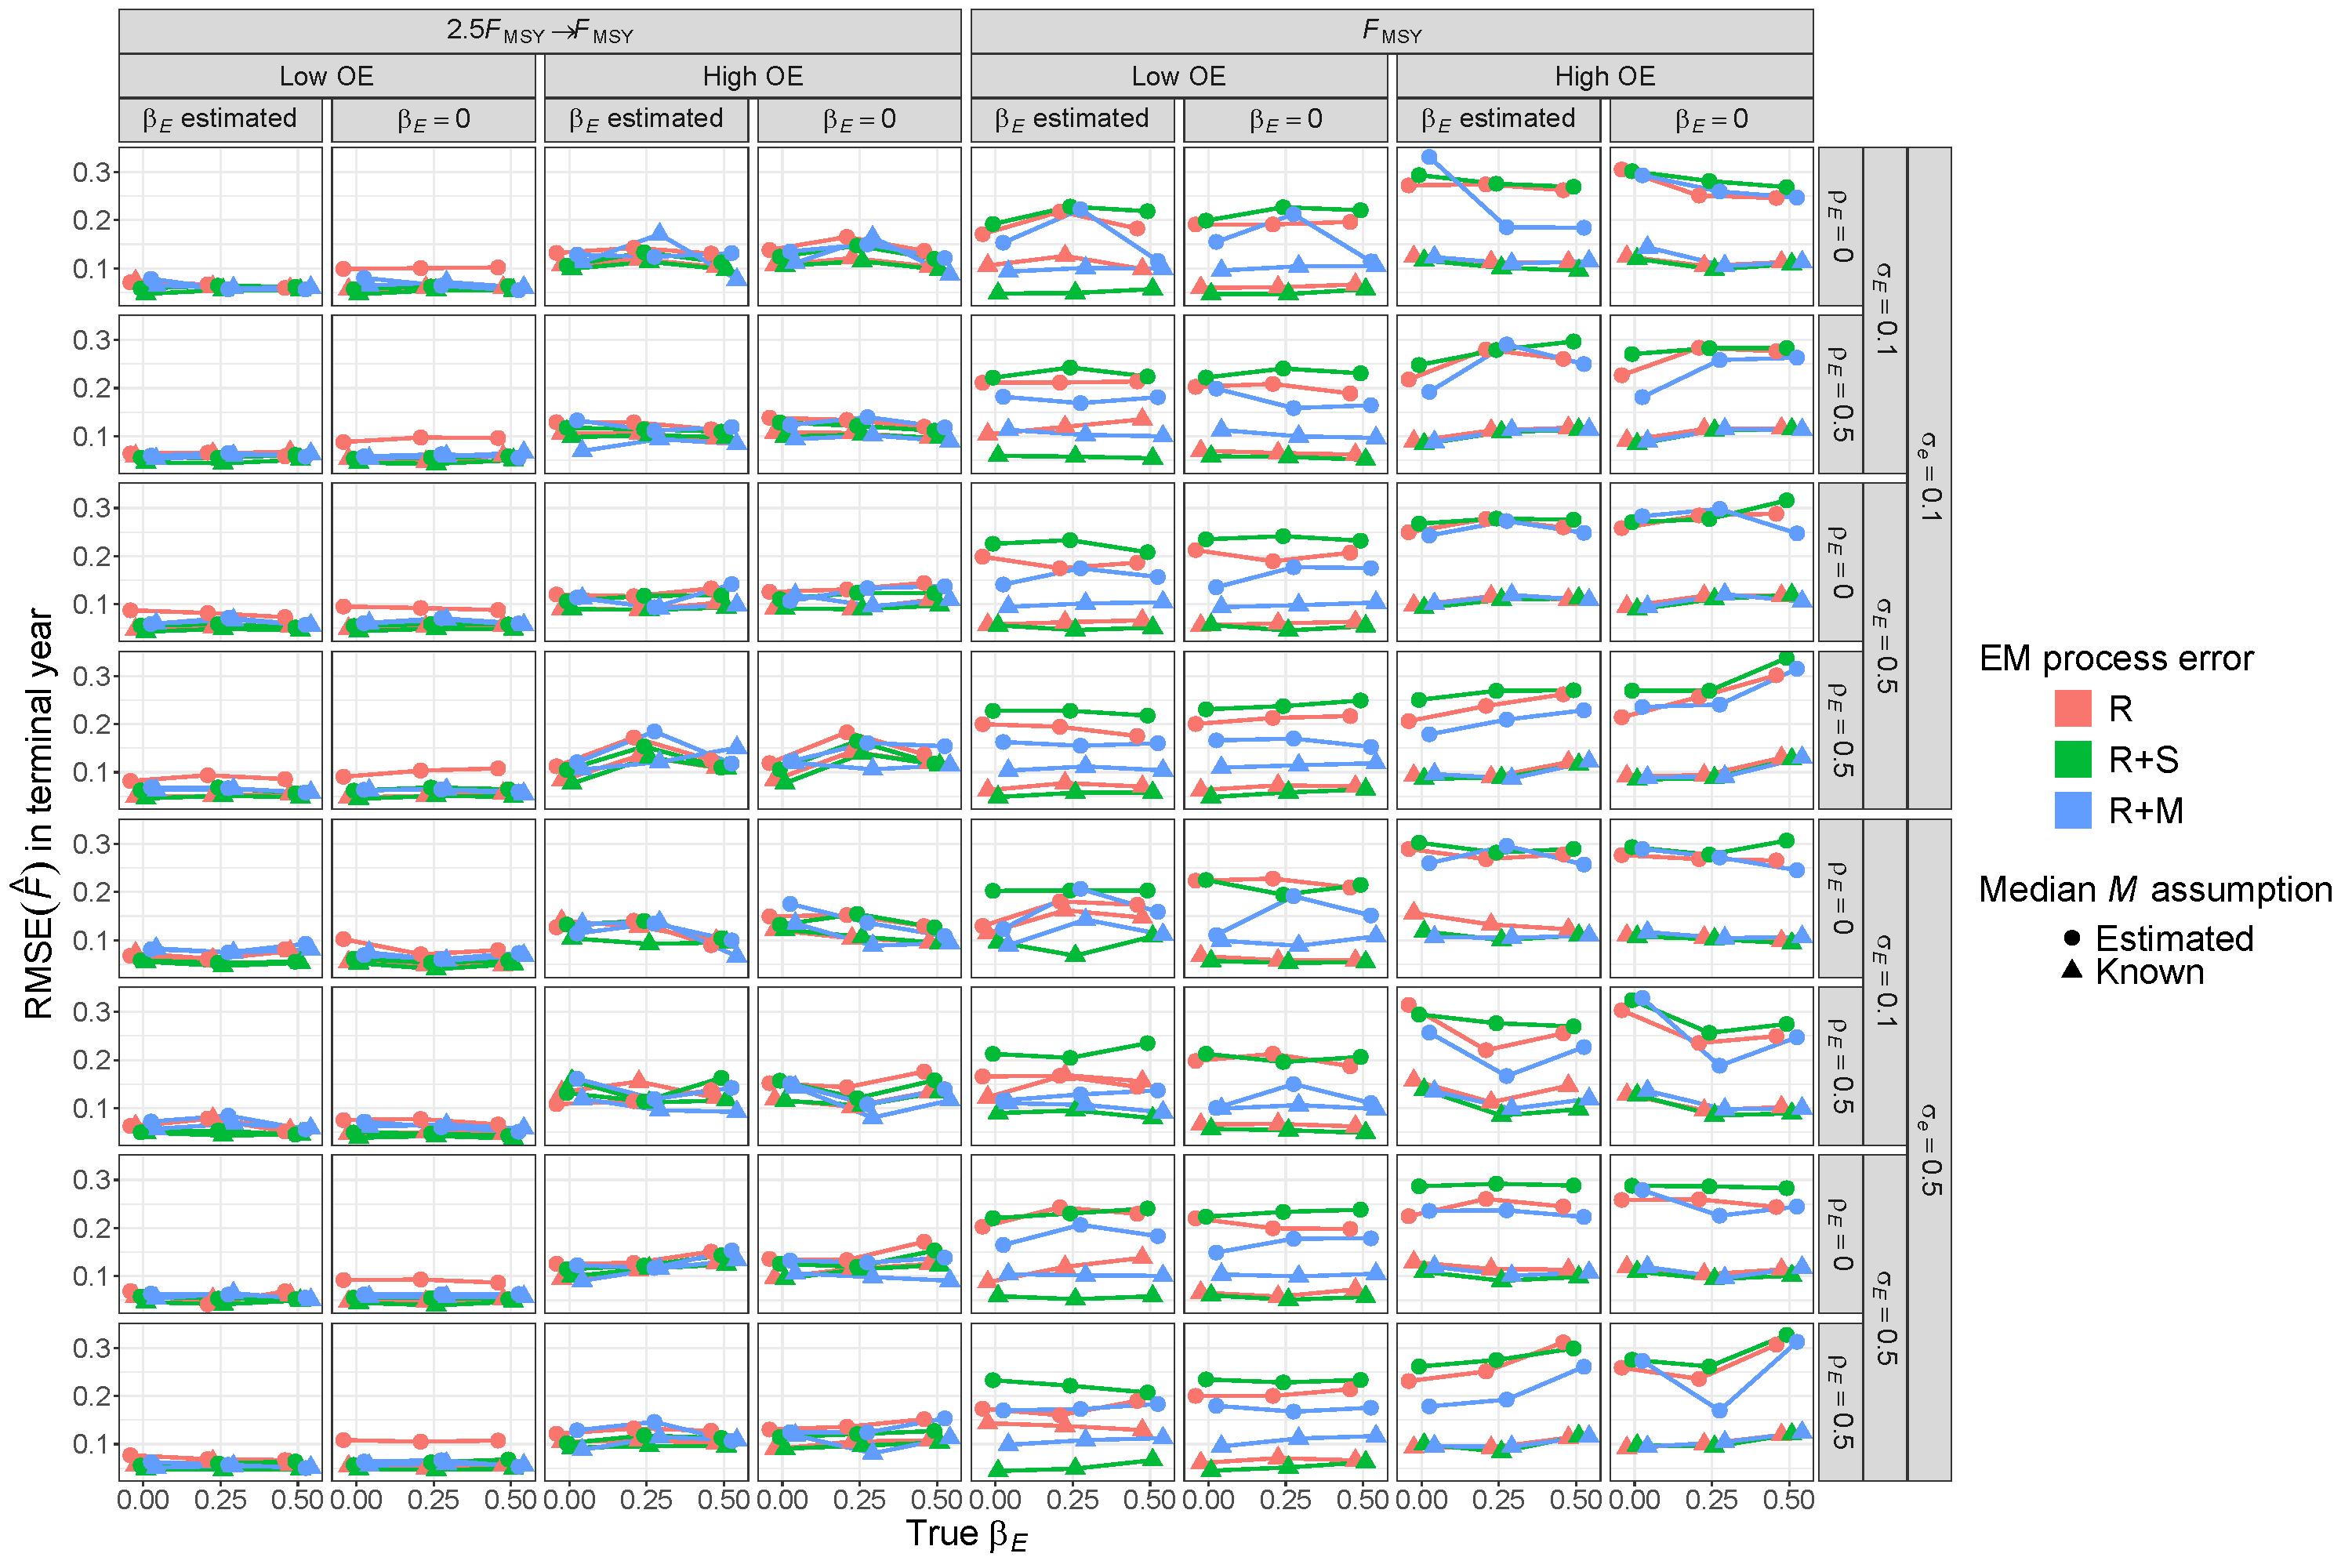
\includegraphics[height = \textheight]{terminal_year_F_rmse_RSom}
\end{center}
\caption{For R+S \DIFdelbeginFL \DIFdelFL{OMs}\DIFdelendFL \DIFaddbeginFL \DIFaddFL{operating models}\DIFaddendFL , RMSE of estimates of fully-selected fishing mortality ($F$)  in the terminal year for \DIFdelbeginFL \DIFdelFL{EMs }\DIFdelendFL \DIFaddbeginFL \DIFaddFL{estimating models }\DIFaddendFL with alternative process error assumptions, treatment of covariate effect ($\beta_E = 0$ or estimated), and treatment of median $M$ parameter ($\beta_M$ estimated or known).}\label{terminal_F_rmse_RSom}
\end{figure}
\end{landscape}

\begin{landscape}
\begin{figure}
\begin{center}
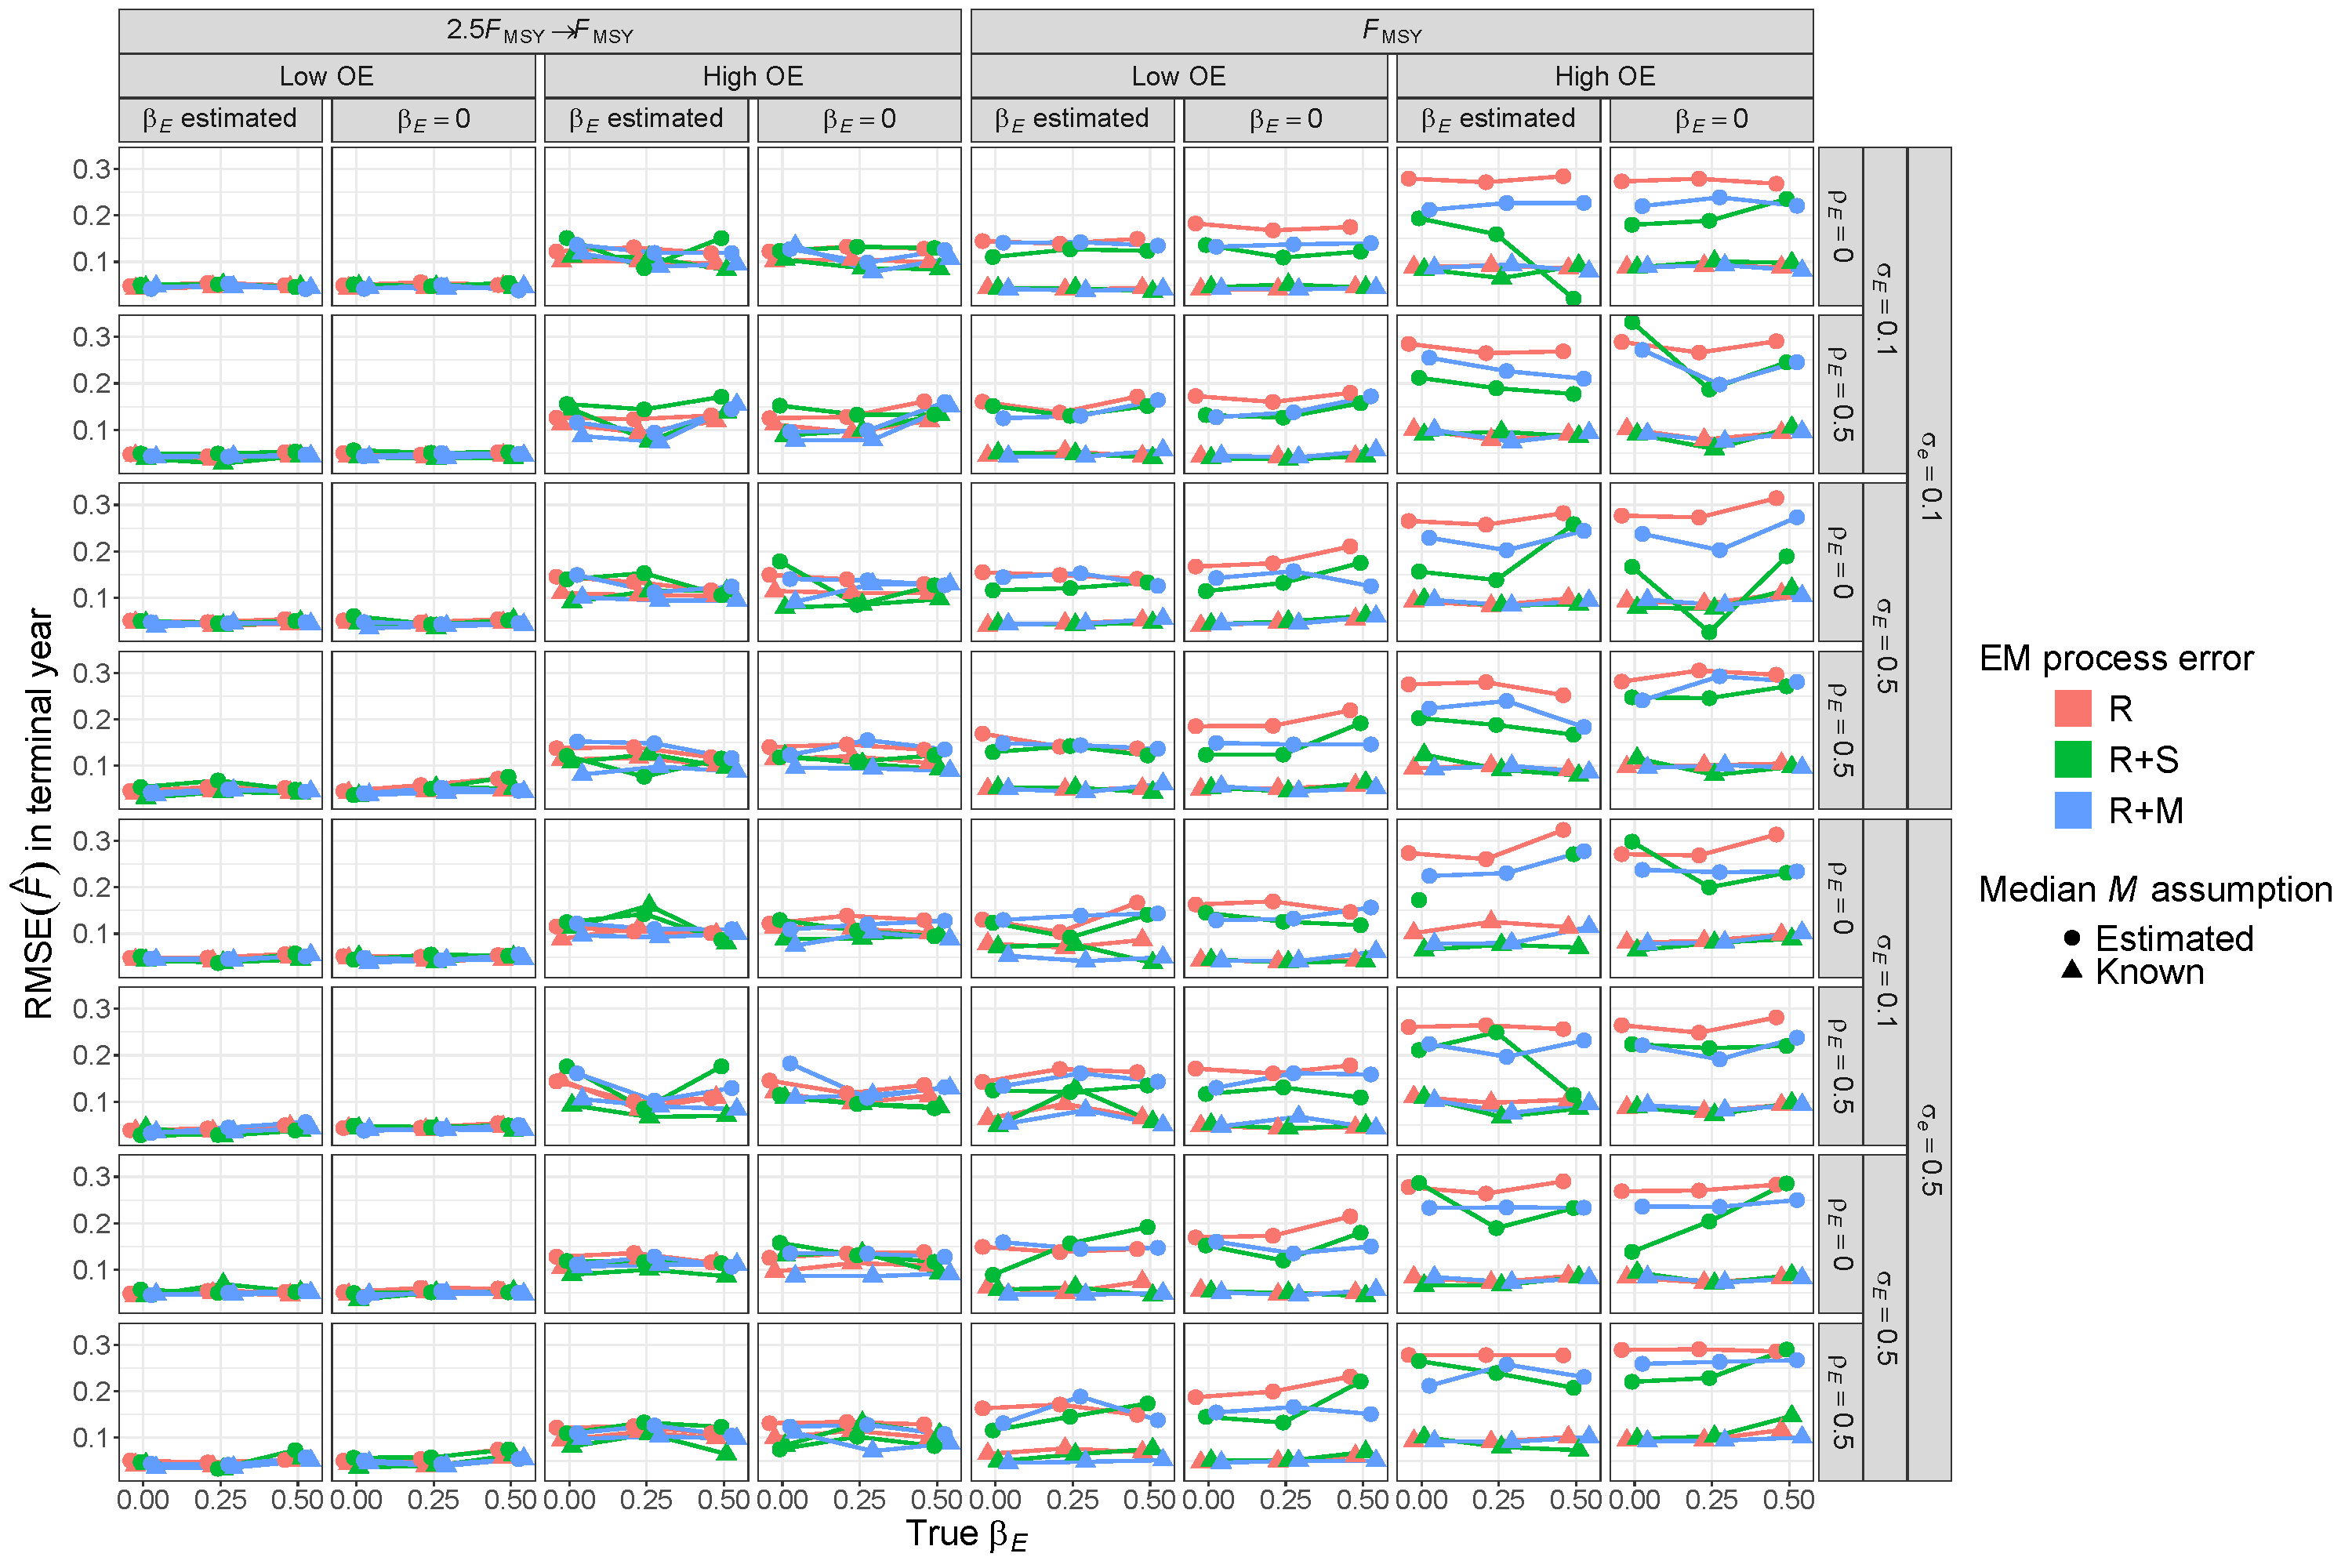
\includegraphics[height = \textheight]{terminal_year_F_rmse_RMom}
\end{center}
\caption{For R+M \DIFdelbeginFL \DIFdelFL{OMs}\DIFdelendFL \DIFaddbeginFL \DIFaddFL{operating models}\DIFaddendFL , RMSE of estimates of fully-selected fishing mortality ($F$)  in the terminal year for \DIFdelbeginFL \DIFdelFL{EMs }\DIFdelendFL \DIFaddbeginFL \DIFaddFL{estimating models }\DIFaddendFL with alternative process error assumptions, treatment of covariate effect ($\beta_E = 0$ or estimated), and treatment of median $M$ parameter ($\beta_M$ estimated or known).}\label{terminal_F_rmse_RMom}
\end{figure}
\end{landscape}

\end{document}
